\chapter{Relaxation et Équilibre dans les Systèmes Quantiques Intégrables : Une Approche par la Thermodynamique de Bethe}\label{chap:relaxation}
\minitoc

%------------------------------------------------------------------
\section*{Introduction générale}

Dans les modèles quantiques intégrables, l’évolution vers l’équilibre, à partir d’un état initial arbitraire (et typiquement hors d’équilibre), ne conduit pas à une thermique de Gibbs classique.  
En effet, du fait de l’existence d’une infinité de charges conservées en involution, les systèmes intégrables n’explorent qu’une sous-partie contrainte de l’espace des états accessibles.  
Ils relaxent alors vers un état stationnaire décrit par une \emph{Ensemble Thermodynamique Généralisé} (GGE), qui encode la conservation de toutes ces quantités.

Cette section pose les fondations nécessaires à la description de ces états stationnaires dans le cadre de la \textbf{thermodynamique de Bethe} (TBA), qui généralise l’analyse au-delà de l’état fondamental.  
Nous considérons ici un régime macroscopique à température (ou entropie) finie, correspondant à des états hautement excités du spectre, mais toujours décrits dans le formalisme intégrable exact.

Notre point de départ est la relation constitutive entre la \emph{densité de quasi-particules} (ou \emph{rapidités}) $\rho(\theta)$ et la \emph{densité d’états} disponibles $\rho_s(\theta)$, qui encode le spectre accessible en présence d’interactions.  
Nous introduisons ensuite une opération clé de la TBA, appelée \emph{habillage} (\emph{dressing}), qui intervient systématiquement dans le calcul des observables physiques et permet de prendre en compte de manière non perturbative les effets des interactions.  
Cette construction sera illustrée dans le cadre du modèle intégrable de Lieb–Liniger, qui décrit un gaz unidimensionnel de bosons avec interaction delta répulsive.

Les outils développés ici seront fondamentaux pour formuler dans la section suivante le concept d’ensemble généralisé (GGE), et pour décrire la dynamique de relaxation des systèmes intégrables.



\section{Notion d’état d’équilibre généralisé (GGE)}

\paragraph{Introduction.}


\paragraph{Configuration des états.}\label{sec:config-etats}.
On désigne par $\boldsymbol{\{ \theta_a \}}\equiv \{ \theta_1 , \cdots , \theta_{N} \}$ la \emph{configuration de rapidités} caractérisant un état propre à $N\!\equiv\!N(\{ \theta_a \})$ particules – le nombre de particules n’est donc pas fixé \emph{a priori} mais dépend de la configuration.  
L’état propre correspondant est noté $\ket{\{ \theta_a \}}\;=\;\ket{\{\theta_1,\dots,\theta_N \}}$.

%%%%%%%%%%%%%%%%%%%%%%%%%%%%%%%%%%%%%%%%%%%%%%%%%%
\paragraph{Observables diagonales dans la base des états propres.}
Dans le chapitre précédent (\ref{chap:LL-BA}), on a vu que l'état $\ket{\{ \theta_a \}}$ associé à cette configuration est une état propre des observables nombre et quantité de mouvement  et  énergie cinétique \eqref{chap1:eq.Q.P.K.theta.1}. Ces observables sont diagonales dans la base des états propres :
\begin{eqnarray}
	\operator{Q}  =  \sum_{ \{\theta_a\} } \left ( \sum_{a = 1}^{N}  1 \right )  \vert \{ \theta_a\}\rangle	\langle \{ \theta_a \}\vert, \, 
	\operator{P}  =  \sum_{\{ \theta_a\}}\left( \sum_{a = 1}^{N}  \theta_a \right )   \vert \{ \theta_a\}\rangle	\langle \{ \theta_a \}\vert,\,\operator{K}  =  \sum_{\{ \theta_a\}}\left ( \sum_{a = 1}^{N} \frac{\theta_a^2}{2} \right )   \vert \{ \theta_a\}\rangle	\langle \{ \theta_a \}\vert.\label{chap.2.gge.1}		
\end{eqnarray}
avec $ \sum_{\{ \theta_a\}}$ une somme sur tous les configurations.\\
%\begin{eqnarray}
%	\operator{Q} \ket{\{ \theta_a\}}  =  \sum_{ \{\theta_a\} } \left ( \sum_{a = 1}^{N}  1 \right ) \ket{\{ \theta_a\}}, \, 
%	\operator{P} \ket{\{ \theta_a\}}  =  \sum_{\{ \theta_a\}}\left( \sum_{a = 1}^{N}  \theta_a \right ) \ket{\{ \theta_a\}},\,\operator{H} \ket{\{ \theta_a\}}  =  \sum_{\{ \theta_a\}}\left ( \sum_{a = 1}^{N} \frac{\theta_a^2}{2} \right )   \ket{\{ \theta_a\}}.		
%\end{eqnarray}

Nous avons introduit ces observables en injectant des opérateurs $\operator{f}$ proportionnels à des puissances de la quantité de mouvement d’une particule $\operator{p}$, respectivement $\propto \operator{p}^0$, $\propto \operator{p}^1$ et $\propto \operator{p}^2$, dans l’opérateur à un corps $\operator{F}$ défini dans l’équation \eqref{chap.1:eq.rapel.opp.1.second.2}. Écrit de cette manière, nous avons vu dans l’équation \eqref{chap.1:eq.rapel.opp.1.second.3} que pour $\operator{f} = \operator{p}^q$ avec $q$ entier, l’état de Bethe $\ket{\{ \theta_a \} }$ est un état propre de $\operator{F}$ :
\begin{eqnarray}\label{chap.2:eq.rapel.opp.1.second.1}
	 \operator{F} \ket{\{\theta_a\}} =   \sum_{ \{\theta_a\} }\left( \sum_{a = 1}^N \theta_a^q \right) \ket{\{\theta_a\}},
\end{eqnarray}
avec des valeurs propres données par des puissances de $\theta$. Cela motive l’étude d’états d’équilibre statistique au-delà de l’équilibre thermique, c’est-à-dire au-delà de l’ensemble de Gibbs.
   




%%%%%%%%%%%%%%%%%%%%%%%%%%%%%%%%%%%%%%%%%%%%
\paragraph{Contexte et GGE dans les systèmes intégrables.}

Dans un système quantique {\bf intégrable}, il existe une infinité de charges conservées locales $\operator{Q}_i$ commutant entre elles et avec l’Hamiltonien $\operator{H}$ ([Rigol et al. 2007] ) \cite{??}. Concrètement, chaque charge se présente sous la forme $\operator{Q}_i = \int dx \,\operator{q}_i(x)$, où $\operator{q}_i(x)$ est une densité d’observable locale à support borné. L’intégrabilité implique ainsi une caractérisation complète des états propres par un ensemble de paramètres (rapidités $\{\theta_j\}$ dans le modèle de Lieb-Liniger) \cite{??}. En particulier, contrairement aux systèmes génériques, un système intégrable ne thermalise pas au sens canonique classique, car la présence de toutes ces contraintes empêche l’oubli complet des conditions initiales. Les points clés sont alors :

\begin{itemize}[label = $\bullet$]
	\item {\bf Charges conservées} : infinité de locales $\operator{Q}_i$ satisfaisant et $[\operator{Q}_i , \operator{H} ] = 0$ et $[\operator{Q}_i , \operator{Q}_j ] = 0$.
	\item {\bf Densités locales} : chaque $\operator{Q}_i$ s’écrit $\operator{Q}_i = \int_\mathbb{R} dx \, \operator{q}_i(x)$ avec $\operator{q}_i(x)$ à support fini.
	\item {\bf Relaxation non canonique} : après un {\em quench} (changement brutal de paramètre), le système évolue vers un état stationnaire qui n’est pas décrit par l’ensemble canonique habituel.
\end{itemize}

Pour décrire cet état, on introduit l’{\bf ensemble de Gibbs généralisé (GGE)}. Rigol et al. ont montré qu’une « extension naturelle de l’ensemble de Gibbs aux systèmes intégrables » prédit correctement les valeurs moyennes des observables après relaxation \cite{??}.  Formellement, pour une région finie du système $\mathcal{S} \subset \mathbb{R}$, on définit la matrice densité locale :
\begin{eqnarray}
	\operator{\rho}^{(\mathcal{S})}_{\mathrm{GGE}} = \frac{1}{Z^{(\mathcal{S})}}\exp \left ( - \sum_i \beta_i \operator{Q}_i^{(\mathcal{S})} \right), \quad \operator{Q}_i^{(\mathcal{S})} = \int_\mathcal{S} dx \, \operator{q}_i(x), \label{chap.TBA.op.rho.S}	
\end{eqnarray}

où $\beta_i \in \mathbb{R}$ sont les multiplicateurs de Lagrange (ou « températures généralisées ») associés aux charges locales conservées $\{\operator{Q}_i\}$. La fonction de partition 
\begin{eqnarray}
	Z^{(\mathcal{S})} = \bm{\mathrm{Tr}}\left [\exp \left( - \sum_i \beta_i \operator{Q}_i^{(\mathcal{S})} \right ) \right ]  \label{chap.TBA.op.Z.S}	
\end{eqnarray}
 assure la normalisation. L’{\bf état GGE} ainsi défini est le seul permettant de prédire de manière cohérente les observables locales de $\mathcal{S}$ à long temps \cite{??}. Autrement dit, l’équilibre local après quench est un état stationnaire faisant perdurer la mémoire de chaque charge conservée, ce qui conduit à un nombre macroscopique de paramètres $\beta_i$ thermodynamiques (une « température » par charge) \cite{??}.

 \subparagraph{Interprétation des multiplicateurs de Lagrange.}
Les multiplicateurs de Lagranges $\beta_i$ apparaissent naturellement lors de l'optimisation sous contraintes, par exemple dans le formalisme de l'{\bf ensemble de Gibbs généralisé (GGE)}, oû il imposent la conservation des valeurs moyennes des charges $\langle \operator{Q}_i^{(\mathcal{S})} \rangle_{\operator{\rho}^{(\mathcal{S})}_{\mathrm{GGE}}} = \bm{\mathrm{Tr}}[\operator{\rho}^{(\mathcal{S})}_{\mathrm{GGE}} \operator{Q}_i^{(\mathcal{S})}]   $.\\

En résumé, la GGE généralise les ensembles canoniques standard : au lieu de retenir uniquement l’énergie, on impose la conservation de l’ensemble complet $\{\operator{Q}_i \}$. Cette construction rend compte du fait que, dans un système intégrable, les observables locaux convergent vers les valeurs moyennes de $\operator{\rho}^{(\mathcal{S})}_{\mathrm{GGE}}$ , et non vers celles d’un Gibbs thermique ordinaire \cite{??}\cite{??}. On comprend ainsi pourquoi la {\em thermalisation habituelle} (canonique ou microcanonique) échoue : seul l’ensemble de Gibbs généralisé peut intégrer toutes les contraintes locales.

\paragraph{Rappel sur le modèle de Lieb-Liniger et distribution de rapidités.}
Comme rappelé au chapitre précédent, {\bf le modèle de  Lieb-Liniger} (gaz bosonique 1D à interactions de contact) est un exemple paradigmatique d’un système intégrable \cite{??}. Ses états propres sont caractérisés par un ensemble de $N$  rapidités $\{ \theta_a \}$ , qui jouent le rôle de quasi-momenta ({\bf Bethe ansatz}). Dans ce contexte, l’état macroscopique du gaz après relaxation unitaire est entièrement déterminé par la {\bf distribution des rapidités}. Formellement, on définit $\rho(\theta)$ la distribution intensive des rapidités telle que $\rho(\theta) d \theta$ donne la fraction de particules par unité de longueur ayant une rapidité dans la cellule $[\theta , \theta + d \theta ] $.\\

Cette « distribution de rapidités » est d’autant plus pertinente qu’elle est {\em accessible expérimentalement}. En effet, lorsque le gaz bosonique 1D est libéré et laissé s’étendre, la distribution asymptotique des vitesses des atomes coïncide avec la distribution initiale des rapidités \cite{??} . Autrement dit, la GGE prédit un profil de vitesses observables en laboratoire. Léa Dubois souligne dans sa thèse que " la distribution de rapidités est la distribution asymptotique des vitesses des atomes après une expansion dans le guide 1D ", et qu’elle peut être extraite par l’hydrodynamique généralisée \cite{??}. \\

Dans la GGE, cette distribution macroscopique $\rho(\theta)$ est fixée par l’ensemble des charges conservées. Par exemple, on ajuste les $\beta_i$ de sorte que les valeurs moyennes $\langle \operator{Q}_i \rangle_{\operator{\rho}^{(\mathcal{S})}_{\mathrm{GGE}}}$ correspondent aux valeurs initiales. Ce processus détermine donc la fonction $\rho(\theta)$ décrivant l’état d’équilibre local. Les observables locaux du gaz (densité, corrélations, etc.) en découlent alors via les équations de Bethe ansatz. 


\paragraph{Convention pour les moyennes d'observables.}
Dans la suite du chapitre, nous noterons la moyenne d’une observable $\operator{\mathcal{O}}$ dans un état décrit par une matrice densité (ici noté) $\operator{\rho}$ par :
\begin{eqnarray}\label{chap.TBA.moy.dens}	
	\braket{\operator{\mathcal{O}}}_{\operator{\rho}} \doteq \bm{\mathrm{Tr}}[\operator{\rho} \, \operator{\mathcal{O}}],
\end{eqnarray}
En particulier, si la matrice densité est un projecteur, comme $\ket{\{\theta_a \}}\!\bra{\{\theta_a \}}$, $\bm{\mathrm{Tr}}[\ket{\{\theta_a \}}\!\bra{\{\theta_a \}} \operator{\mathcal{O}}] =  \bra{\{\theta_a \}}\operator{\mathcal{O}}\ket{\{\theta_a \}}$. dans ce cas on notera la moyenne :
\begin{eqnarray}\label{chap.TBA.moy.dens.pur}
	\braket{\operator{\mathcal{O}}}_{\{\theta_a \}} = \bra{\{\theta_a \}} \operator{\mathcal{O}} \ket{\{\theta_a \}},
\end{eqnarray}
où l’on note simplement l’ensemble des rapidité ${\theta_a}$ pour désigner l’état pur.

%%%%%%%%%%%%%%%%%%%%%%%%%%%%%%%%%%%%%%%%%%%%%%%%%%
\paragraph{Charges conservées locales diagonales dans la base des états propres.}
Les charges conservées locales $\operator{Q}_i^{(\mathcal{S})}$ est diagonale dans la base des  états propres $\ket{ \{ \theta_a \}}$ , avec pour valeurs propres $\langle \operator{Q}_i^{(\mathcal{S})} \rangle_{\{\theta_a \}} $ 	 :
%\begin{eqnarray}
%	\operator{Q}_i^{(\mathcal{S})} & = & \sum_{ \{\theta_a\} } \langle \operator{Q}_i^{(\mathcal{S})} \rangle_{\{\theta_a \}}  \ket{\{\theta_a \}}\!\bra{\{\theta_a \}}.		
%\end{eqnarray}
\begin{eqnarray}\label{chap.TBA.Qi.diag}
	\operator{Q}_i^{(\mathcal{S})}\ket{\{\theta_a \}} & = &  \langle \operator{Q}_i^{(\mathcal{S})} \rangle_{\{\theta_a \}}  \ket{\{\theta_a \}}.		
\end{eqnarray}
%%%%%%%%%%%%%%%%%%%%%%%%%%%%%%%%%%%%%%%%
\paragraph{Probabilité d’un état à rapidités fixées.}
On peut alors définir la probabilité d’occurrence d’un état $\ket{\{ \theta_a \} }$ comme la moyenne de la matrice densité locale $\operator{\rho}^{(\mathcal{S})}_{\mathrm{GGE}}$ définie dans \eqref{chap.TBA.op.rho.S}:
\begin{eqnarray}
	\mathbb{P}^{(\mathcal{S})}_{\{ \theta_a \}}  & \equiv &  \langle \operator{\rho}^{(\mathcal{S})}_{\mathrm{GGE}} \rangle_{\{\theta_a \}}, \label{chap.TBA.P.1}\\
	& = & 
	\frac{1}{Z^{(\mathcal{S})}} \exp \left (- \sum_i \beta_i \langle \operator{Q}_i^{(\mathcal{S})} \rangle_{\{\theta_a \}} \right ) \label{chap.TBA.P.2}.
\end{eqnarray}

%%%%%%%%%%%%%%%%%%%%%%%%%%%
\paragraph{Moyenne d’un charges conservées locales et dérivées de $Z^{(\mathcal{S})}$.} Les charges locales $\operator{Q}_i^{(\mathcal{S})}$ sont diagonale dans la bases \( \{ \ket{\{\theta_a \}} \}  \) [cf eq~ ~\eqref{chap.TBA.Qi.diag}]. 
On peut donc  écrire la moyenne d’une observable comme une somme pondérée par cette probabilité [cf eqs ~\eqref{chap.TBA.P.1}-\eqref{chap.TBA.P.2}] , ou encore comme une dérivée de la fonction de partition définie dans l'équation \eqref{chap.TBA.op.Z.S} :
\begin{eqnarray}
	\langle \operator{Q}_i^{(\mathcal{S})} \rangle_{\operator{\rho}^{(\mathcal{S})}_{\mathrm{GGE}}} &= & \sum_{\{ \theta_a\}} \langle \operator{Q}_i^{(\mathcal{S})} \rangle_{\{\theta_a \}} \mathbb{P}^{(\mathcal{S})}_{\{ \theta_a \}} \label{chap.TBA.moy.1}\\
	 & = &  \left. \frac{1}{Z^{(\mathcal{S})}} \frac{\partial Z^{(\mathcal{S})}}{\partial \beta_i} \right )_{\beta_{j \neq i }}	 \label{chap.TBA.moy.2}
\end{eqnarray}

Par le même raisonnement le moment non centré s'écrit :
\begin{eqnarray}
	\braket{ \operator{Q}_{i_1}^{(\mathcal{S})} \, \operator{Q}_{i_2}^{(\mathcal{S})} \cdots \operator{Q}_{i_q}^{(\mathcal{S})} }_{\operator{\rho}^{(\mathcal{S})}_{\mathrm{GGE}}} &= &  (-1)^q \frac{1}{Z^{(\mathcal{S})}} \left.\frac{\partial}{\partial \beta_{i_1}} \right )_{\beta_{j \neq i_1 }} \left.\frac{\partial}{\partial \beta_{i_2}} \right )_{\beta_{j \neq i_2 }} \cdots \left.\frac{\partial}{\partial \beta_{i_q}} \right )_{\beta_{j \neq i_q }} Z^{(\mathcal{S})} \label{chap.TBA.mom.1}.	
\end{eqnarray}

%%%%%%%%%%%%%%%%%%%%%%%%%%%%%%%
\paragraph{Moments d’ordre supérieur et fluctuations.} On s'avance sur le chapitre (\ref{chap:Fluctu}).
Le premier et second moments permettent d’accéder à la variance 
\begin{eqnarray}
	 \left \langle \left (\operator{Q}_i^{(\mathcal{S})} - \langle\operator{Q}_i^{(\mathcal{S})} \rangle_{\operator{\rho}^{(\mathcal{S})}_{\mathrm{GGE}}} \right )^2  \right \rangle_{\operator{\rho}^{(\mathcal{S})}_{\mathrm{GGE}}} = \langle(\operator{Q}_i^{(\mathcal{S})})^2 \rangle_{\operator{\rho}^{(\mathcal{S})}_{\mathrm{GGE}}}  -  \langle\operator{Q}_i^{(\mathcal{S})} \rangle_{\operator{\rho}^{(\mathcal{S})}_{\mathrm{GGE}}}^2	
\end{eqnarray}
de le charge locale $\operator{Q}_i^{(\mathcal{S})}$, en injectant \eqref{chap.TBA.moy.2} et \eqref{chap.TBA.mom.1} et en utilisant $\frac{1}{f} \partial_x^2 f - ( \frac{1}{f} \partial_x f ) = \partial_x^2 \ln f  $:
\begin{eqnarray}
	\left \langle \left (\operator{Q}_i^{(\mathcal{S})} - \langle\operator{Q}_i^{(\mathcal{S})} \rangle_{\operator{\rho}^{(\mathcal{S})}_{\mathrm{GGE}}} \right )^2  \right \rangle_{\operator{\rho}^{(\mathcal{S})}_{\mathrm{GGE}}}  &=&	  \left . \frac{\partial^2 \ln Z^{(\mathcal{S})}  }{{\partial \beta_i}^2 }  \right )_{\beta_{j\neq i}},\\
	& = &  - \left . 	\frac{\partial \langle\operator{Q}_i^{(\mathcal{S})} \rangle_{\operator{\rho}^{(\mathcal{S})}_{\mathrm{GGE}}} }{\partial \beta_i } \right )_{\beta_{j\neq i}}.	
\end{eqnarray}

%%%%%%%%%%%%%%%%%%%%%%%%%%%%%%
\paragraph{Cas particulier de l’équilibre thermique.}

Dans le cas particulier de l’équilibre thermique standard (\ie Gibbsien), le système est décrit par une seule contrainte d’énergie (ou d’énergie et de particule, dans le cas d’un grand canonique). Les multiplicateurs de Lagrange associés aux charges conservées peuvent alors être identifiés à des grandeurs thermodynamiques classiques.

\begin{itemize}[label=$\bullet$]
	\item Si la seule charge conservée est le nombre de particules $\operator{Q}_0^{(\mathcal{S})} = \operator{Q}$, le multiplicateur associé est $\beta_0 = -\beta \mu$, où $\mu$ est le potentiel chimique et $\beta = T^{-1}$ l’inverse de la température (avec $k_B = 1$).
	
	\item Si la charge conservée est $\operator{Q}_2^{(\mathcal{S})}-\mu\operator{Q}_0^{(\mathcal{S})}  = \operator{K} - \mu \operator{Q} $ (ensemble grand canonique), alors le multiplicateur est simplement $ \beta$.
\end{itemize}

Dans le cadre de l’équilibre thermique , les moyennes et les fluctuations thermodynamiques usuelles s’expriment naturellement comme dérivées du logarithme de la fonction de partition $Z^{(\mathcal{S})}$ :
\begin{eqnarray}
	\langle \operator{Q} \rangle_{\operator{\rho}^{(\mathcal{S})}_{\mathrm{GGE}}}  = \left .\frac{1}{\beta} \frac{ \partial \ln Z^{(\mathcal{S})}}{\partial \mu } \right )_{T},  & &  \left . \frac{1}{\beta} \frac{ \partial \langle \operator{Q} \rangle_{\operator{\rho}^{(\mathcal{S})}_{\mathrm{GGE}}}}{\partial \mu } \right )_{T} =  \left . \frac{1}{\beta^2} \frac{ \partial^2 \ln Z^{(\mathcal{S})}}{{\partial \mu}^2 } \right )_{T} \\
	\langle \operator{H} - \mu\operator{Q}  \rangle_{\operator{\rho}^{(\mathcal{S})}_{\mathrm{GGE}}}  = -\left . \frac{ \partial \ln Z^{(\mathcal{S})}}{\partial \beta } \right )_{\mu} ,  & & -\left .  \frac{ \partial \langle \operator{H} - \mu\operator{Q} \rangle_{\operator{\rho}^{(\mathcal{S})}_{\mathrm{GGE}}}}{\partial \beta } \right )_{\mu } = \left .  \frac{ \partial^2 \ln Z^{(\mathcal{S})}}{{\partial \beta}^2 } \right )_{\mu}   .		
\end{eqnarray}
En combinant ces relations, on peut également exprimer l’énergie moyenne et ses fluctuations comme :
\begin{eqnarray}
	\langle \operator{H} \rangle_{\operator{\rho}^{(\mathcal{S})}_{\mathrm{GGE}}}  = \left [ \left .\frac{\mu}{\beta} \frac{ \partial}{\partial \mu } \right )_{T} -\left . \frac{ \partial }{\partial \beta } \right )_{\mu}   \right ]\ln Z^{(\mathcal{S})},  \quad  -\left .  \frac{ \partial \langle \operator{H} \rangle_{\operator{\rho}^{(\mathcal{S})}_{\mathrm{GGE}}}}{\partial \beta } \right )_{-\mu \beta } = \left [ \left .\frac{\mu}{\beta} \frac{ \partial}{\partial \mu } \right )_{T} -\left . \frac{ \partial }{\partial \beta } \right )_{\mu}  \right ]^2\ln Z^{(\mathcal{S})}.		
\end{eqnarray}

%%%%%%%%%%%%%

\section{Remarques sur le formalisme}




%% !TEX encoding = IsoLatin

%\documentclass[11pt,a4paper]{report}
%\documentclass[11pt,a4paper]{book}
\documentclass[10pt, titlepage]{book} % Taille de base des caractères (12pt recommandée pour lecture)


% -------------------------------------
% Encodage et langue
% -------------------------------------
\usepackage[utf8]{inputenc}
\usepackage[T1]{fontenc}
\usepackage[french]{babel}

% -------------------------------------
% Marges et dimensions
% -------------------------------------
\usepackage[a4paper, top=3.0cm, bottom=3.0cm, left=3cm, right=3cm]{geometry} 
% Ajuste ici les marges selon tes préférences

% -------------------------------------
% Interligne
% -------------------------------------
\usepackage{setspace}
%\onehalfspacing  % Interligne 1.5 
%\doublespacing %(utilise \doublespacing pour double interligne)

% -------------------------------------
% Police (facultatif)
% -------------------------------------
%\usepackage{mathptmx} % Police Times (ancienne)
%\usepackage{libertine} % Police élégante
%\usepackage{newtxtext,newtxmath} % Times moderne pour texte et maths

% -------------------------------------
% Paquets utiles
% -------------------------------------
\usepackage{amsmath, amssymb, amsthm}
\usepackage{graphicx}
\usepackage{hyperref}
\usepackage{xcolor}
\usepackage{braket}
\usepackage{tikz}
\usepackage{pgfplots}
\usepackage{float}
\usepackage{enumitem}
\usepackage{caption}
\usepackage{subcaption}
\usepackage{algorithm2e}
\usepackage{cancel}
\usepackage{bm}
\usepackage{listings}
\usepackage{pdfpages}
\usepackage{mdframed}
\usepackage{braket}
\usepackage{stmaryrd} 
\usetikzlibrary {datavisualization}
\usetikzlibrary {arrows.meta,bending,positioning}
\usetikzlibrary {datavisualization.formats.functions}
%PREAMBULE pour schÃéma
\usepackage{pgfplots}
\usepackage{tikz}
\usepackage[european resistor, european voltage, european current]{circuitikz}
\usetikzlibrary{arrows,shapes,positioning}
\usetikzlibrary{decorations.markings,decorations.pathmorphing,
decorations.pathreplacing}
\usetikzlibrary{calc,patterns,shapes.geometric}
\usepackage{anyfontsize}


% -------------------------------------
% Pour les chapitres
% -------------------------------------
\usepackage[Glenn]{fncychap} % Style de chapitres


% -------------------------------------
% Largeur du texte (évite de le redéfinir si tu utilises geometry)
% -------------------------------------
%\setlength\textwidth{20.5cm}
%\setlength\textheight{22cm}

% -------------------------------------
% Optionnel : si tu veux jouer avec les marges manuellement
% -------------------------------------
% \setlength\topmargin{-1cm}
% \setlength\evensidemargin{-2cm}
% \setlength\oddsidemargin{\evensidemargin}

\usepackage{mdframed}

\usepackage{scalerel}
\usepackage{xcolor}
\usepackage{stackengine}
\usepgflibrary {shadings}


\usetikzlibrary {decorations.pathmorphing}

\usepackage{tikz}

\usepackage{marvosym}
\usepackage{changepage}

\usepackage{minitoc}
\usepackage{tocloft}
%\renewcommand{\cfttoctitle}{\hspace{-2em}}
% Nastaveni obsahu
% Nastaveni obsahu

\usepackage{imakeidx}
\usepackage{fancyhdr}

%\usepackage{makeidx}
\makeindex[intoc=true]
\makeindex[name=pers, title=Index of person names, intoc=true]

\usepackage{xcolor}

\usepackage{hyperref}

%%%%%%%%%%%%%%%%%%%%%
%\definecolor{linkcolor}{RGB}{0,0,180}
\usepackage{titlesec}

\usepackage{tocloft}
\usepackage{datetime} % Pour une date personnalisée
\usepackage[useregional]{datetime2}

\usepackage{mathrsfs}

% -------------------------------------
% Pour les mini-tables des matières
% -------------------------------------
\usepackage{minitoc}
\dominitoc

%\usepackage[most]{tcolorbox}

%%%%%%%%%%%%%%%%%%%%%%%%%%%%%
%\usepackage[utf8]{inputenc}
%\usepackage[T1]{fontenc}
%\usepackage[french]{babel}
%\usepackage{amsmath, amssymb}
%\usepackage{graphicx}
%\usepackage{hyperref}
%\usepackage{tikz}
%\usepackage{physics}
%\usepackage{float}


%\newcommand{\ket}[1]{\left|#1\right\rangle}
%\newcommand{\bra}[1]{\left\langle#1\right|}
%\newcommand{\mean}[1]{\left\langle#1\right\rangle}
%\newcommand{\dd}{\mathrm{d}}

% Activer \frontmatter, \mainmatter et \appendix pour la classe report
%\newcommand{\frontmatter}{%
%  \pagenumbering{roman}%
%  \setcounter{page}{1}%
%  \renewcommand{\chaptermark}[1]{\markboth{##1}{}}
%  \renewcommand{\sectionmark}[1]{\markright{##1}}
%}
%
%\newcommand{\mainmatter}{%
%  \pagenumbering{arabic}%
%  \setcounter{page}{1}
%}


% \appendix est déjà défini dans report, inutile de le redéfinir


% Figures flottantes:
% fraction maximale d'une page pouvant etre occupe par une figure:
\renewcommand{\topfraction}{0.8}
% fraction minimale d'une page reservee pour le texte:
\renewcommand{\textfraction}{0.2}
% fraction minimale d'occupation de la page par une figure pleine page:
\renewcommand{\floatpagefraction}{0.7}

%%%%%%%%%%%%%%%%%%%%%%%%%%%%%%%%%%%%%%%%
%         D\'ecoupage des mots           %
%%%%%%%%%%%%%%%%%%%%%%%%%%%%%%%%%%%%%%%%
\hyphenation{}

%%%%%%%%%%%%%%%%%%%%%%%%%%%%%%%%%%%%%%%%
%%%%  Th\'eor\`emes, d\'efinitions, etc.
%%%%%%%%%%%%%%%%%%%%%%%%%%%%%%%%%%%%%%%%


% Il y a diffÃérents types d'ÃénoncÃés qui mÃéritent un environnement spÃécifique, voici une liste assez exhaustive.
\theoremstyle{plain}
    \newtheorem{Theo}{Th\'eor\`eme}[section] %compteur commençant par le numÃéro de la section (on pourrait aussi faire commencer par le numÃéro de la sous-section - remplacer "section" par "subsection")
    \newtheorem{Prop}[Theo]{Proposition}        %mÃême compteur que pour les thÃéorÃèmes
    \newtheorem{Prob}[Theo]{Probl\`eme}        %idem
    \newtheorem{Lemm}[Theo]{Lemme}            %etc...
    \newtheorem{Coro}[Theo]{Corollaire}
    \newtheorem{Propr}[Theo]{Propri\'et\'e}
    \newtheorem{Conj}[Theo]{ Conjecture}
    \newtheorem{Aff}[Theo]{Affirmation}

    \newtheorem{TheoPrinc}{Th\'eor\`eme}     %compteur spÃécifique pour les thÃéorÃèmes les plus importants du papier
        
\theoremstyle{definition}
    \newtheorem{Defi}[Theo]{D\'efinition}
    \newtheorem{Exem}[Theo]{Exemple}
    \newtheorem{Nota}[Theo]{\Large Notation}

\theoremstyle{remark}
    \newtheorem{Rema}[Theo]{Remarque}
    \newtheorem{NB}[Theo]{N.B.}
    \newtheorem{Comm}[Theo]{Commentaire}
    \newtheorem{question}[Theo]{$\ast$ Question}
    \newtheorem{exer}[Theo]{Exercice}
    \newtheorem{Consequence}[Theo]{Conséquence}
    \newtheorem{Rap}[Theo]{Rappel}
    \newtheorem*{Merci}{Remerciements}

\mdfdefinestyle{propstyle}{%
linecolor=black,linewidth=2pt,%
hidealllines=true,
frametitlerule=true,%
frametitlebackgroundcolor=gray!20,
backgroundcolor=gray!10!white,
roundcorner=5pt,
innertopmargin=\topskip,
}

%\mdtheorem[style=propstyle]{prop}{Property}[chapter]
\mdtheorem[style=propstyle]{lemma}[prop]{Lemma}
\mdtheorem[style=propstyle]{TheoPrinc}{Th\'eor\`eme}[chapter]

% Définition d'un style personnalisé pour les Affirmations
\mdfdefinestyle{affirmestyle}{%
    linecolor=gray, % Couleur de la bordure
    linewidth=1pt, % Épaisseur de la bordure
    backgroundcolor=gray!10, % Couleur de fond (gris clair)
    roundcorner=5pt, % Coins arrondis
    innertopmargin=0pt, % Marge intérieure au-dessus du cadre
    innerbottommargin=10pt, % Marge intérieure en-dessous du cadre
    innerleftmargin=10pt, % Marge intérieure à gauche
    innerrightmargin=10pt, % Marge intérieure à droite
    skipabove=10pt, % Espace au-dessus du cadre
    skipbelow=10pt % Espace en-dessous du cadre
}

% Définition de l'environnement Affirmation
\theoremstyle{definition} % Style de théorème pour les affirmations
\newmdtheoremenv[style=affirmestyle]{aff}{Point clé n$^{\circ}$} % Environnement Affirmation avec le style personnalisé
    
\newcommand\dangersign[1]{%
    \renewcommand\stacktype{L}%
    \scaleto{\stackon[1.3pt]{\color{red}$\triangle$}{\tiny !}}{#1}%
}

\tikzset{every picture/.style={execute at begin picture={\shorthandoff{:;!?};}}}
\tikzstyle{every picture}+=[remember picture]
\tikzstyle{na} = [shape=rectangle,inner sep=0pt]

% Commandes pour les flèches textuelles
\newcommand{\ptFleche}[2]{        % Déclaration d'une extrémité de flèche
    \tikz[baseline=(#1.base)]\node[na](#1){#2};
  }
%\newcommand{\Fleche}[5][thick]{    % Dessin de la flèche
%    \begin{tikzpicture}[overlay]
%        \path[->,#1](#2) edge [out=#4, in=#5] (#3);
%    \end{tikzpicture}
%  }
  
% \newcommand{\Flecheprim}[5][thick]{    % Dessin de la flèche
%    \begin{tikzpicture}[overlay]
%        \path[->,#1](#2) edge [out=#4, in=#5] (#3);
%    \end{tikzpicture}
%  }
%

\definecolor{linkcolor}{RGB}{0,0,180}
\PassOptionsToPackage{
    colorlinks=true,
    linkcolor=linkcolor,
    citecolor=linkcolor,
    urlcolor=linkcolor
}{hyperref}

% Appliquer la couleur à tous les niveaux de titre
\titleformat{\section}{\normalfont\color{linkcolor!90!black}\Large\bfseries}{\thesection}{1em}{}
\titleformat{\subsection}{\normalfont\color{linkcolor!70!black}\large\bfseries}{\thesubsection}{1em}{}
\titleformat{\subsubsection}{\normalfont\color{linkcolor!50!black}\normalsize\bfseries}{\thesubsubsection}{1em}{}
\titleformat{\paragraph}[runin]{\normalfont\color{linkcolor!30!black}\bfseries}{\theparagraph}{1em}{}
\titleformat{\subparagraph}[runin]{\normalfont\color{linkcolor!10!black}\itshape}{\thesubparagraph}{1em}{}
%%%%%%%%%%%%%%%%%%%%%%%

%%Couleurs dans la table des matières

% Modifier la couleur des entrées de la TOC
\renewcommand{\cftsecfont}{\color{linkcolor!90!black}}
\renewcommand{\cftsubsecfont}{\color{linkcolor!70!black}}
\renewcommand{\cftsubsubsecfont}{\color{linkcolor!50!black}}
\renewcommand{\cftparafont}{\color{linkcolor!30!black}}
\renewcommand{\cftsubparafont}{\color{linkcolor!10!black}}
%%%%%%%%%%%%%%%%%%%%%%%%%%%%%
% Reglages:
%
%\pagestyle{fancyplain}
%\addtolength{\headwidth}{\marginparsep}
%\addtolength{\headwidth}{\marginparwidth}
%\renewcommand{\chaptermark}[1]{\markboth{#1}{}}
%\renewcommand{\sectionmark}[1]{\markright{\thesection\ #1}}
%\lhead[\fancyplain{}{\bfseries\thepage}]{}
%\rhead[]{\fancyplain{}{\bfseries\thepage}}
%\chead[\fancyplain{}{\bfseries\leftmark}]{\fancyplain{}{\bfseries\rightmark}}
%\cfoot{}
%

%usepackage{titlesec}
% Changer la couleur des paragraphes en rouge par exemple :
%\titleformat{\paragraph}[runin] % ou [block] selon ce que tu veux
%  {\normalfont\color{red}\bfseries}
%  {\theparagraph}{1em}{}

%%% ===== Index principal + index secondaire (noms propres) =====
\makeindex[intoc=true]
\makeindex[name=pers, title=Index des noms propres, intoc=true]

%%% ===== Couleur des liens =====
\definecolor{linkcolor}{RGB}{0,0,180}
\PassOptionsToPackage{
    colorlinks=true,
    linkcolor=linkcolor,
    citecolor=linkcolor,
    urlcolor=linkcolor
}{hyperref}
\usepackage{hyperref}

%%% ===== Réglages hyperref =====
\hypersetup{
  pdftitle={Étude de la dynamique hors équilibre de bosons unidimensionnels},
  pdfsubject={Quantum Physics},
  pdfauthor={Guillaume THEMEZE <guillaume.themeze@gmail.fr>},
  pdfkeywords={LaTeX, quantum, bosons, dynamique},
  colorlinks=true
}

%%% ===== Style des titres (colorés) =====
\titleformat{\chapter}[display]{\normalfont\sffamily\huge\bfseries\color{black}}{\chaptertitlename\ \thechapter}{20pt}{\Huge}
\titleformat{\section}{\normalfont\color{linkcolor!90!black}\Large\bfseries}{\thesection}{1em}{}
\titleformat{\subsection}{\normalfont\color{linkcolor!70!black}\large\bfseries}{\thesubsection}{1em}{}
\titleformat{\subsubsection}{\normalfont\color{linkcolor!50!black}\normalsize\bfseries}{\thesubsubsection}{1em}{}
\titleformat{\paragraph}[runin]{\normalfont\color{linkcolor!30!black}\bfseries}{\theparagraph}{1em}{}
\titleformat{\subparagraph}[runin]{\normalfont\color{linkcolor!10!black}\itshape}{\thesubparagraph}{1em}{}

%%% ===== Couleurs de la table des matières =====
\renewcommand{\cftsecfont}{\color{linkcolor!90!black}}
\renewcommand{\cftsubsecfont}{\color{linkcolor!70!black}}
\renewcommand{\cftsubsubsecfont}{\color{linkcolor!50!black}}
\renewcommand{\cftparafont}{\color{linkcolor!30!black}}
\renewcommand{\cftsubparafont}{\color{linkcolor!10!black}}

%%% ===== En-têtes et pieds de page =====
\pagestyle{fancy}
\fancyhf{}
\setlength{\headheight}{14pt}

\fancyhead[RO,LE]{\thepage}
\fancyhead[LO]{\scshape \nouppercase{\rightmark}}  % Section
\fancyhead[RE]{\scshape \nouppercase{\leftmark}}  % Chapitre
\renewcommand{\headrulewidth}{.4pt}


\newdateformat{mydate}{\THEDAY~\monthname[\THEMONTH]~\THEYEAR}
\newdateformat{mydatetime}{\THEDAY~\monthname[\THEMONTH]~\THEYEAR~à~\currenttime}

%\DTMsetstyle{french} % ou autre style
%\DTMsetup{showtimezone=false}

\fancyfoot[L]{Thèse}
%\fancyfoot[R]{Paris, \mydatetime\today{} -- Période 2022--2025}
\fancyfoot[R]{Paris, \DTMnow -- Période 2022--2025}
%\fancyfoot[R]{Paris, le \DTMdate\today{} à \DTMcurrenttime -- Période 2022--2025}
\renewcommand{\footrulewidth}{.4pt}

% Supprimer les numéros sur la première page de chaque chapitre
\makeatletter
\let\ps@plain=\ps@empty
\makeatother

%%% ===== Réglages des titres de sections dans les en-têtes =====
\renewcommand{\chaptermark}[1]{\markboth{#1}{}}
\renewcommand{\sectionmark}[1]{\markright{\thesection\ #1}}

%%% ===== Notes de bas de page à la française =====
\usepackage[french]{babel}
%\usepackage[frenchfootnotes]{french}
%\FrenchFootnotes
%\AddThinSpaceBeforeFootnotes

%%%%%%%%%%%%%%%%%%%%%%%%%%%%%%%%%%
\newcommand{\operatorvec}[1]{\vec{{\bm{#1}}}} % pour les operateur
\newcommand{\operator}[1]{\hat{\bm{#1}}} % pour les operaeur vecteur
\newcommand{\operatormat}[1]{\operatorname{#1}} % pour les operaeur vecteur
\newcommand{\operatortilde}[1]{\tilde{\bm{#1}}} % pour les opetateur avec un tilde
\newcommand{\operatortildevec}[1]{\tilde{\bm{#1}}}% pour les opetateur avec un tilde et vecteur
\newcommand{\dfonc}[1]{\mathscr{D}_{[#1]}}
%%%%%%%%%%%%%%%%%%%%%%%%%%%%%%%%%%


% Commandes spécifiques ou pour la mise en forme



\title{Titre de la thèse}
\author{Prénom NOM}
\date{\today}



\begin{document}



\frontmatter
\chapter*{Introduction générale}
\addcontentsline{toc}{chapter}{Introduction générale}
%\minitoc
%\section*{....}

Ceci est l’introduction de la thèse.


\tableofcontents
\bigskip
\mainmatter

\chapter{Modèle de Lieb-Liniger et approche Bethe Ansatz}\label{chap:LL-BA}
\minitoc


%\section*{Introduction}
%
%Dans ce chapitre, nous introduisons progressivement le modèle de Lieb-Liniger et l'Ansatz de Bethe, outils fondamentaux pour décrire un gaz de bosons unidimensionnel avec interactions delta. L'objectif est d'accompagner pas à pas le lecteur depuis la formulation du problème quantique en champ de bosons jusqu'aux solutions exactes obtenues par l'Ansatz de Bethe.
%
%Pour des raisons pédagogiques, nous commençons par aborder le cas d’une seule particule, sans interaction, avec des condition aux bord périodique. Cela permet d’introduire naturellement les fonction d'onde à une particule, leur évolution sous l’action du Hamiltonien libre et l'équation qui reluste de la condition de limite periodique ( equation de bethe à une. particule) : la premier quantification.
%
%Puis nous continions par écrire l'équation du champ de bosons, exprimée à l’aide des opérateurs de création et d’annihilation en représentation de position : la seconde quantification. Cela permet de mettre au clair les operateur à un corps et à 2 corps.
%
%Une fois les notations bien établies, nous généralisons le raisonnement au cas de \(N\) particules, pour obtenir l’Hamiltonien de Lieb-Liniger complet ainsi que la forme générale de l’Ansatz de Bethe. Les solutions ainsi construites permettent non seulement de déterminer le spectre de l’Hamiltonien, mais aussi de calculer des observables physiques importantes, telles que l’impulsion totale ou le nombre de particules.
%
%Ensuite, nous étudions le cas de deux particules, cette fois en tenant compte de l’interaction locale. Ce qui nous permet de metre en évidence les consequences de des interaction ponctiels sur entre autre la continuté de la fonction d'onde et que l'on a pour une équatuion de Bethe à deux particule.%Cela nous amène à considérer les états de position dans le cas général, y compris lorsque les deux particules peuvent occuper la même position. Cette situation, bien plus subtile qu’il n’y paraît, met en évidence la complexité introduite par l’interaction, et justifie que l’on commence par analyser les configurations où les particules sont à des positions distinctes.
%
%%Dans le référentiel du centre de masse, le problème à deux corps avec interaction devient équivalent à un problème à une seule particule en interaction avec une barrière delta au centre. Cette reformulation permet d’interpréter l’effet de l’interaction comme une condition de raccord sur la fonction d’onde, tout en respectant la symétrie bosonique.
%
%%Nous revenons ensuite aux coordonnées du laboratoire afin d’introduire naturellement la forme des solutions imposée par l’Ansatz de Bethe. Cela nous conduit aux équations dites de Bethe, qui relient les quasimoments des particules à travers des conditions de périodicité modifiées par l’interaction.
%
%Ensuitre nous généralisont la fonction d'on à deux particule, à la fonction d'onde à N particule. Et les les quation de bethe à N particume
%
%Enfin, nous introduisons la notion de distribution de rapidité, outil essentiel dans l’étude des états d’énergie minimale (états fondamentaux) et au delà de l'éta fondamentale. Ce cadre servira de base aux développements ultérieurs sur les gaz bosons intégrables.

\section*{Introduction}

Ce chapitre est consacré à la présentation progressive du modèle de Lieb-Liniger et de l’Ansatz de Bethe, outils centraux pour la description d’un gaz de bosons unidimensionnel en interaction via un potentiel de type delta. L’objectif est d’accompagner rigoureusement le lecteur depuis la formulation quantique du système jusqu’aux solutions exactes obtenues par l’approche de Bethe.

\medskip

Nous commençons, pour des raisons pédagogiques, par le cas le plus simple : une particule libre, sans interaction, dans un espace unidimensionnel avec conditions aux bords périodiques. Cette première étape permet d’introduire naturellement les fonctions d’onde à une particule, leur évolution sous l’action du Hamiltonien libre, ainsi que la quantification résultant des conditions de périodicité — autrement dit, la version élémentaire des équations de Bethe.

\medskip

Nous passons ensuite à la formulation du problème en champ quantique, en exprimant le Hamiltonien en termes d’opérateurs de création et d’annihilation dans la représentation positionnelle : il s’agit du passage à la seconde quantification. Cette étape permet de formaliser clairement les termes à un corps et à deux corps dans l’Hamiltonien, et d’établir les notations qui seront utilisées tout au long du chapitre.

\medskip

Une fois ce cadre posé, nous généralisons le raisonnement au cas de \(N\) particules pour introduire le modèle complet de Lieb-Liniger. Nous présentons alors l’Ansatz de Bethe dans sa forme générale, qui fournit les états propres de l’Hamiltonien. Ce formalisme permet d’accéder explicitement au spectre du système, ainsi qu’à diverses quantités physiques telles que l’impulsion totale et le nombre de particules.

\medskip

Nous traitons d'abord le cas à seulement deux particules, cette fois en tenant compte de l’interaction locale. L’analyse de ce système met en lumière les effets de l’interaction ponctuelle sur la régularité de la fonction d’onde et les conditions de raccord, ainsi que sur les modifications des équations de Bethe. Ce cas constitue une étape clé vers la généralisation à \(N\) particules.

\medskip

La fonction d’onde est ensuite étendue au cas général de \(N\) particules, ce qui nous permet de dériver les équations de Bethe pour un système entièrement interactif. Ces équations encapsulent toute l’information sur les états propres du système.

\medskip

Enfin, nous introduisons la notion de \emph{distribution de rapidité}, concept fondamental pour la description des états dans la limite thermodynamique. Elle permet non seulement de caractériser les états d’énergie minimale (états fondamentaux), mais aussi d’analyser des configurations excitées au-delà de l’état fondamental. Ce formalisme constituera le socle des développements ultérieurs sur les propriétés thermodynamiques et dynamiques des gaz bosoniques intégrables.


\section{Description du modèle de Lieb-Liniger}

\subsection{Introduction au modèle de gaz de Bose unidimensionnel}% et Hamiltonien du modèle}

\subsubsection{De la première à la seconde quantification}

\paragraph{Introduction.}

La mécanique quantique se développe historiquement en deux grandes étapes : la \emph{première quantification}, aussi appelée quantification canonique, et la \emph{seconde quantification}. Comprendre ces deux cadres est essentiel pour aborder les systèmes quantiques complexes, en particulier ceux où le nombre de particules peut varier.

%La mécanique quantique s’est historiquement développée en deux étapes : la \emph{première quantification}, aussi appelée quantification canonique, puis la \emph{seconde quantification}. Comprendre ces deux cadres est essentiel pour aborder les systèmes à nombre de particules variable.


%\vspace{0.5cm}

\paragraph{Première quantification (quantification canonique, particule unique).}

La première quantification est la mécanique quantique standard, celle que vous avez rencontrée dès vos premiers cours. Elle consiste à quantifier un système classique décrit par des variables dynamiques telles que la position $x$ et la quantité de mouvement $p$. On procède en remplaçant ces variables par des {\bf opérateurs hermitiens} $\operator{x}$ et %$\operator{p}$
\begin{eqnarray}
	\operator{p} \doteq -i\hbar \operator{\partial}_x,	\label{chap.1.rapel.1}
\end{eqnarray}
où $\hbar$ est la constante de Planck réduite, satisfaisant la {\bf relation de commutation canonique} fondamentale $[\operator{x}, \operator{p}] = i\hbar$. L’état du système est alors décrit par une {\bf fonction d’onde} $\psi(x,t)$, solution de {\bf l’équation de  Schrödinger} indépendante du nombre de particules :
\begin{eqnarray}
\quad i \hbar \frac{\partial \psi }{\partial t}  &= \operator{\mathcal{H}} \psi,\label{chap.1.rapel.2}
\end{eqnarray}

avec $\operator{\mathcal{H}}$ l’opérateur hamiltonien. 

\begin{mdframed}[
	linewidth=0.5pt, 
	backgroundcolor=gray!5, 
	roundcorner=50pt,	
	innerleftmargin=5pt,
    innerrightmargin=5pt,
    innertopmargin=-10pt,
    innerbottommargin=2pt,
    leftmargin=2pt,
    rightmargin=2pt
	]
\subparagraph{Exemple : particule libre en une boite à une dimension.} 
	{~}\\
	
	Dans le cas d’une particule libre de masse $m$ se déplaçant en une dimension, l’Hamiltonien est constitué uniquement du terme cinétique $\operator{\mathcal{H}} = \operator{p}^2 / 2m$. En représentation position, où l’opérateur quantité de mouvement s’écrit comme dans l’équation \eqref{chap.1.rapel.1}, l’Hamiltonien prend alors la forme différentielle :
	\begin{eqnarray}
		\operator{\mathcal{H}} = -\frac{\hbar^2}{2m} \partial_x^2.\label{chap.1.rapel.libre.1}
	\end{eqnarray}
	Les états propres stationnaires de \eqref{chap.1.rapel.2} dépendant du temps sont de la forme $\psi_k(x,t) = \varphi_k(x)\,e^{-i\varepsilon(k)t/\hbar}$ où $\varphi_k(x)$ est une fonction propre de l’hamiltonien,  soit de  l’équation stationnaire  $\operator{\mathcal{H}}\varphi_k = \varepsilon(k)\varphi_k$ \ie pour une particule libre:
	\begin{eqnarray}
		\frac{\hbar^2}{2m} \partial_x^2 \varphi_k = \varepsilon(k) \varphi_k,\label{chap.1.rapel.libre.2}
	\end{eqnarray}
	avec $\varepsilon(k)$ l’énergie associée à une onde plane de nombre d’onde $k$
	\begin{eqnarray}
		\varepsilon(k) = \frac{\hbar^2 k^2 }{2 m}\label{chap.1.rapel.libre.3}.
	\end{eqnarray}
	Les fonctions propres spatiales $\varphi_k(x)$ de l’hamiltonien libre s’écrivent comme des combinaisons linéaires d’ondes planes  
	\begin{eqnarray}
		\varphi_k(x) = a e^{-i k x} + b e^{i k x},~~ \mbox{avec}\quad  (a,b) \in \mathbb{C}^2\label{chap.1.rapel.libre.4}.
	\end{eqnarray}
\subparagraph{Périodisité.}
	Si la particule est confinée dans une boîte de longueur $L$ avec des conditions aux limites périodiques (ie $\varphi_k(x+L) = \varphi_k(x)$), alors le spectre de $k$ est quantifié : 
	\begin{eqnarray}
		e^{kL}= 1 \quad\mbox{ou encore} kL \in 2\pi\mathbb{Z}\label{chap.1.rapel.libre.5}.
	\end{eqnarray}
	Le problème est équivalent à celui d’une particule libre sur un cercle de périmètre $L$.\\
	
	\medskip
	
	La particule est délocalisée sur tout l’espace (le cercle), sans structure particulière \ie le solutions \eqref{chap.1.rapel.libre.4} correspondent à des {\bf états non liés} (ou états de diffusion).

%On résume :
%\begin{eqnarray}
%	,~~ , ~~\varphi_k(x) = a e^{-i k x} + b e^{i k x},~~ kL \in 2\pi\mathbb{Z}.\label{chap.1.recap}
%\end{eqnarray}
\end{mdframed}

\medskip

Pour $k \neq 0 $ (respectivement pour $k = 0$), la fonction propre $\varphi_k(x)$ de l’équation \eqref{chap.1.rapel.libre.4} appartient à un sous-espace propre associé à $k$ de dimension 2 (respectivement de dimension 1) engendré par $x \mapsto e^{-ikx}$ et $x \mapsto e^{ikx}$ (respectivement par $x \mapsto 1$).
L’espace engendré par l’ensemble des sous-espaces propres forme un {\bf espace de Hilbert} , muni du {\bf produit scalaire} défini par :
\begin{eqnarray}
	( \varphi_{k'} , \varphi_{k} ) = \int_0^L \varphi_{k'}^\ast(x) \varphi_{k}(x) \, dx .\label{chap.1.rapel.libre.6}
\end{eqnarray}
Les sous-espaces propres sont orthogonaux entre eux \ie en utilisant les conséquences de la condition de périodicité \eqref{chap.1.rapel.libre.5}, $( \varphi_{k'} , \varphi_{k} ) = 0$ pour $\vert k' \vert \neq \vert k \vert  $ . 
Pour chaque sous-espace propre on impose que les états propres forment une base orthonormale \ie en utilisant \eqref{chap.1.rapel.libre.5}, les fonctions propres $\varphi_{k}$ écrit sous la forme \eqref{chap.1.rapel.libre.4}, sont orthogonaux avec $\varphi_{\overline{k}} \colon x \mapsto \pm ( b^\ast e^{-ikx} - a^\ast e^{ikx} )$  soit $(\varphi_{\overline{k}} , \varphi_{k} ) = 0$, et on impose que  $ \vert a \vert^2 + \vert b \vert^2 = L^{-1}$ pour assuré la normalité  de $\varphi_{k}$  et de $\varphi_{\overline{k}}$ soit  $( \varphi_{k} , \varphi_{k} ) = (\varphi_{\overline{k}} , \varphi_{\overline{k}})   = 1$. 

\medskip

Les solutions générales de l’équation de Schrödinger s’écrivent alors comme une superposition d’états propres  $\psi = c_0 \psi_0 +  \sum_{\vert k \vert > 0 } (c_k \psi_k  + c_{\overline{k}} \psi_{\overline{k}}) $. 

\medskip
Il y a deux base de vecteur propre particulier : 
\begin{enumerate}[label=\roman*)]
	\item {\bf Base de chiralité / impulsion :}
%	\begin{eqnarray}
%		\left \{ \begin{array}{rcll} \varphi_+  & = & \displaystyle \frac{1}{\sqrt{L}} e^{+ikx} & \mbox{: état avec impulsion $+\hbar k $ } \\ \varphi_-  & = & \displaystyle \frac{1}{\sqrt{L}}e^{-ikx} & \mbox{: état avec impulsion $-\hbar k $ }\end{array}\right.
%	\end{eqnarray}
	\begin{eqnarray}\label{chap.1.rapel.libre.7}
		\varphi_\pm  & = & \displaystyle \frac{1}{\sqrt{L}} e^{\pm ikx} 
	\end{eqnarray}
	Ces derniers de plus d'être états propres de l’opérateur énergie $\operator{\mathcal{H}}$, sont des états propres de l’opérateur impulsion $\operator{p}$, avec valeurs propres opposées $\pm \hbar k$.
	\item {\bf Base symétrique / antisymétrique :} En appliquant la matrice de passage unitaire  $\frac{1}{\sqrt{2}}\left (\begin{matrix}1 & 1 \\ -i & + i\end{matrix}\right)$ à la base $\{ \varphi_+ , \varphi_- \}$ , on passer dans las base    
%	\begin{eqnarray}
%		\left \{ \begin{array}{rcllll} \varphi_k  &= & \displaystyle\frac{1}{\sqrt{2L}}(e^{+ikx} + e^{-ikx})  & = & \displaystyle \sqrt{\frac{2}{L}} \cos (kx)  & \mbox{type Neumann  : $\varphi_k'(0) = \varphi_k'(L) = 0 $ } \\ \varphi_{\overline{k}}  & = & \displaystyle\frac{1}{\sqrt{2L}i}(e^{+ikx} - e^{-ikx}) & = & \displaystyle \sqrt{\frac{2}{L}} \sin (kx)  & \mbox{type Dirichlet : $\varphi_{\overline{k}}(0) = \varphi_{\overline{k}}(L) = 0 $}\end{array} \right.
%	\end{eqnarray}
	\begin{eqnarray}\label{chap.1.rapel.libre.8}
		\left \{ \begin{array}{rcllll} \varphi_S  & = & \displaystyle \sqrt{\frac{2}{L}} \cos (kx)  & \mbox{type Neumann  : $\varphi_S'(0) = \varphi_S'(L) = 0 $ } \\ \varphi_A   & = & \displaystyle \sqrt{\frac{2}{L}} \sin (kx)  & \mbox{type Dirichlet : $\varphi_A(0) = \varphi_A(L) = 0 $}\end{array} \right.
	\end{eqnarray}
\end{enumerate}


\medskip

Cette condition d’orthonormalité est imposée afin de garantir l’indépendance linéaire des états quantiques, et d'assurer que toute fonction d’onde de l’espace de Hilbert puisse être développée de manière unique sur cette base. 


\medskip

Avec le formalisme de Dirac, la fonction d’onde $\varphi_k$ est représentée par le ket $\ket{k}$ normé (\ie $\langle k' \vert k \rangle = \delta_{k', k}$, où $\delta_{p,q}$ est le symbole de Kronecker)
, et l’équation de Schrödinger s’écrit :
\(
\operator{\mathcal{H}} \ket{k} = \varepsilon(k) \ket{k}.
\)
En appliquant le bra $\bra{x}$ de part et d’autre, on obtient :
\(
\bra{x} \operator{\mathcal{H}} \ket{k} = \varepsilon(k) \langle x \vert k \rangle,
\)
où $\ket{x}$ est normé (\ie $\braket{x'\vert x} = \delta ( x' - x ) $ avec $\delta ( y - x )$ une distribution de Dirac) et $\varphi_k(x) = \langle x \vert k \rangle$ est la représentation positionnelle de l’état $\ket{k}$.


\begin{mdframed}[
	linewidth=0.5pt, 
	backgroundcolor=gray!5, 
	roundcorner=50pt,	
	innerleftmargin=5pt,
    innerrightmargin=5pt,
    innertopmargin=1pt,
    innerbottommargin=2pt,
    leftmargin=2pt,
    rightmargin=2pt
	]
La base $\{\ket{x}\}$ étant continue, et les états $\{\ket{k}\}$ quantifiés (par exemple dans une boîte de taille finie avec conditions aux limites périodiques), les relations de changement de base s’écrivent :
\begin{eqnarray}\label{chap.1:eq.rapel.etat.prim.1}
	\ket{k} = \int_0^L dx \, \varphi_k(x) \ket{x}, \qquad   
	\ket{x} = \sum_k \varphi_k^\ast(x) \ket{k},
\end{eqnarray}
avec $\varphi_k^\ast(x) = \langle k \vert x \rangle$. L’état $\ket{x}$ est relié aux états $\ket{k}$ par une transformation de Fourier discrète. Ces formules montrent que les états $\ket{k}$ sont les composantes de Fourier de l’état $\ket{x}$.
\end{mdframed}


\subparagraph{De la particule unique aux systèmes à $N$ particules.}

Pour un système composé de $N$ particules identiques, une approche naturelle consiste à introduire une fonction d’onde $\varphi(x_1, \dots, x_N)$ dépendant de $N$ variables , symétrique pour des bosons ou antisymétrique pour des fermions sous l’échange de deux coordonnées $x_i \leftrightarrow x_j$, solution de l’équation de Schrödinger à $N$ corps. 
Toutefois, cette description devient rapidement inextricable lorsque le nombre de particules augmente, ou lorsque le système permet la création et l’annihilation de particules, comme dans un milieu ouvert ou en contact avec un bain thermique.


\subsubsection{Seconde quantification}

Pour dépasser ces limitations, on adopte le \textbf{formalisme de la seconde quantification}, dans lequel l’état du système est décrit non plus par une fonction d’onde mais par un vecteur dans un espace de Fock. Les opérateurs de création et d’annihilation remplacent alors les variables dynamiques classiques et permettent une description unifiée et élégante des systèmes à nombre variable de particules.

\paragraph{Structure de l’espace des états de Fock.}
Dans ce formalisme, l’espace des états est une {\bf somme directe d’espaces à $N$ particules}, et chaque état est décrit par l’occupation des différents modes quantiques. Les opérateurs $\operator{a}_k^\dagger$ et $\operator{a}_k$ créent et annihilent une particule dans l’état d’onde plane de moment $k$ :
\begin{eqnarray}
	\ket{k} & = & \operator{a}_k^\dagger \ket{\emptyset} ,%~\equiv~ \text{état avec une particule dans le mode } k,	
\end{eqnarray}
état avec une particule dans le mode $k$ , où \(\ket{\emptyset}\) désigne le vide quantique de Fock, défini par :
\begin{eqnarray}
	\forall k \in \mathbb{R}\colon \qquad \operator{a}_k \ket{\emptyset} = 0 ,\quad  \langle \emptyset \vert \emptyset \rangle = 1. \label{chap:eq.vide.fock.k}
\end{eqnarray}
Le symbole \( \operator{a}_\lambda \) représente ici de manière générique soit l’opérateur \( \operator{b}_\lambda \) pour les bosons, soit \( \operator{c}_\lambda \) pour les fermions, et satisfait respectivement les relations de commutation (pour les bosons) ou d’anticommutation (pour les fermions). Dans ce qui suit, nous nous restreignons au cas bosonique.

\subparagraph{Relations de commutation bosoniques.} Les relations de commutation fondamentales pour les bosons sont :
\begin{eqnarray}
	[\operator{b}_k, \operator{b}_{k'}] = [\operator{b}_k^\dagger, \operator{b}_{k'}^\dagger] = 0 ,\qquad [\operator{b}_k, \operator{b}_{k'}^\dagger] = \operator{\delta}_{k,k'}, \label{chap:1:com.1.k}
\end{eqnarray}
où $\operator{\delta}_{k,k'}$ est le symbole de Kronecker, valant $1$ si $k = k'$ et $0$ sinon.


%\vspace{1em}
\paragraph{Nature du champ quantique.}
La seconde quantification généralise ce cadre en permettant de traiter des systèmes où le nombre de particules n’est pas fixé, ce qui est fréquent en physique des particules, des champs quantiques, ou des gaz quantiques.

L’idée principale est de ne plus quantifier directement les particules, mais le \emph{champ quantique} associé. Les états d’une particule unique deviennent alors des états d’occupation dans un espace de Fock, qui décrit l’ensemble des configurations possibles avec zéro, une, ou plusieurs particules.



\subparagraph{Champs de Bose.}
Le gaz de Bose unidimensionnel est décrit dans le cadre de la théorie quantique des champs par un champ bosonique canonique \( \operator{\Psi}(x) \), qui agit sur l’espace de Fock des états du système. Ce champ quantique encode l’annihilation d’une particule en \( x \), et son adjoint \( \operator{\Psi}^\dag(x) \) correspond à la création d’une particule en ce point. 
\begin{eqnarray}
	\vert x \rangle  & = & \operator{\Psi}^\dag (x)\ket{\emptyset} ,
\end{eqnarray}
état avec une particule en  $x$ et \(\ket{\emptyset}\) est le vide quantique de Fock défini par :
\begin{eqnarray}
	\forall x \in \mathbb{R}, \qquad \operator{\Psi}(x) \ket{\emptyset} = 0. \label{chap:eq.vide.fock}
\end{eqnarray}

\subparagraph{Relations de commutation bosoniques.}
Ces champs satisfont les relations de commutation canoniques à temps égal :
%\begin{eqnarray}
%	\left . \begin{array}{rcl}
%		[ \operator{\Psi}(x),  \operator{\Psi}^\dagger(y) ]  &=&  \operator{\delta}(x - y) \\
%		\left [ \operator{\Psi}(x),  \operator{\Psi}(y) \right ]   =  [ \operator{\Psi}^\dag(x),  \operator{\Psi}^\dag(y) ]  &=&  0 
%	\end{array} \right . \label{chap:1:com.1}
%\end{eqnarray}
\begin{eqnarray}
	 [ \operator{\Psi}(x),  \operator{\Psi}(y)  ]   =  [ \operator{\Psi}^\dag(x),  \operator{\Psi}^\dag(y) ]  =  0,   & & [ \operator{\Psi}(x),  \operator{\Psi}^\dagger(y) ]  =  \operator{\delta}(x - y) ,\label{chap:1:com.1}
\end{eqnarray}
où $\operator{\delta}(x - y)$ est la fonction delta de Dirac.  
Ces relations expriment le caractère bosonique des excitations du champ.

\paragraph{État à $N$ particules.} Soient $N$ bosons dans les états $\{ k_1 , \cdots , k_N \}$ (un boson dans l’état $k_1$, un autre dans $k_2$, etc.) et aux positions $\{ x_1 , \cdots , x_N \}$ (un boson en $x_1$, un autre en $x_2$, etc.). Leurs états s’écrivent alors :
\begin{eqnarray}
	\ket{ \{ k_1 , \cdots , k_N \}} = \frac{1}{\sqrt{N!}} \operator{b}_{k_1}^\dag\, \cdots \, \operator{b}_{k_N}^\dag \ket{\emptyset}, \quad \ket{\{x_1 , \cdots , x_N\}} = \frac{1}{\sqrt{N!}} \operator{\Psi}^\dag(x_1)\, \cdots \, \operator{\Psi}^\dag(x_N) \ket{\emptyset}	, \label{eq.chap.1.ket.N}
\end{eqnarray}
où le facteur \( 1/\sqrt{N!} \) traduit le caractère d’indiscernabilité des bosons et garantit la symétrisation correcte de l’état.

\begin{mdframed}[
	linewidth=0.5pt, 
	backgroundcolor=gray!5, 
	roundcorner=50pt,	
	innerleftmargin=5pt,
    innerrightmargin=5pt,
    innertopmargin=-10pt,
    innerbottommargin=2pt,
    leftmargin=2pt,
    rightmargin=2pt
	]
\subparagraph{Changement de base.}
On peut relier les opérateurs de création/annihilation dans la base des ondes planes aux opérateurs de champ via :
\begin{eqnarray}\label{chap.1:eq.rapel.etat.second.1}
	\operator{b}_k^\dagger = \int_0^L dx \, \varphi_k(x) \operator{\Psi}^\dagger(x), \qquad 
	\operator{\Psi}^\dagger(x) = \sum_k \varphi_k^\ast(x)\operator{b}_k^\dagger.\label{eq.chap.1.TF.1}
\end{eqnarray}
Le champ quantique $\operator{\Psi}(x)$ est relié aux opérateurs de moment $\operator{b}_k$ par une transformation de Fourier. Ces formules montrent que les opérateurs $\operator{b}_{k}$ sont les composantes de Fourier du champ $\operator{\Psi}(x)$.
\end{mdframed}
%où $\varphi_k(x)$ est la fonction d’onde d’un état d’énergie bien définie \( \ket{k} \) dans la représentation positionnelle.
Ainsi, un état à \(N\) bosons dans la base \( \ket{k}^{\otimes N} \) peut s’écrire :
\begin{eqnarray}
	\ket{\{k_a\}} = \frac{1}{\sqrt{N!}} \int dx_1 \cdots dx_N \, \varphi_{\{k_a\}} ( \{x_a\} ) \, \operator{\Psi}^\dag(x_1) \cdots \operator{\Psi}^\dag(x_N) \ket{\emptyset},
\end{eqnarray}
où on note \( \{k_a\} \equiv \{k_1, \dots, k_N\} \) et \( \{x_a\} \equiv \{x_1, \dots, x_N\} \), et la fonction d’onde symétrisée s’écrit :
\(
	\varphi_{\{k_a\}} ( \{x_a\} ) = \frac{1}{\sqrt{N!}} \sum_{\sigma \in \operator{S}_N } \prod_{i=1}^N \varphi_{k_{\sigma(i)}}(x_i),
\) 
avec $\operator{S}_N $  le groupe symétrique d'ordre $N$ mais aussi :
\begin{eqnarray}\label{chap.1:eq.rapel.fonction.propre.N}
	\varphi_{\{k_a\}} (\{x_a\}) = \frac{1}{\sqrt{N!}} \bra{\emptyset} \operator{\Psi}(x_1) \cdots \operator{\Psi}(x_N) \ket{\{k_a\}}.
\end{eqnarray}



\subsubsection{Operateur. }


\paragraph{Opérateur à un corps.}

\subparagraph{Dans la base discrètes des modes \( \{ \ket{k} \} \).}

Soit \( \operator{f} \) un opérateur à une particule, dont les éléments de matrice dans une base orthonormée \( \{ \ket{k} \} \) sont donnés par \( f_{\lambda\nu} = \langle \lambda \vert \operator{f} \vert \nu \rangle \). Un opérateur symétrique à \( N \) particules correspondant à la somme des actions de \( \operator{f} \) sur chacune des particules s’écrit en première configuration  :
\(
	\operator{F} = \sum_{i=1}^N \operator{f}^{(i)},
\)
où \( \operator{f}^{(i)} \) désigne l’action de \( \operator{f} \) sur la $i^\text{e}$ particule uniquement. En base de Dirac, cela donne :
\(
	\operator{f}^{(i)} = \sum_{\lambda, \nu} f_{\lambda\nu} \, \ket{i\!:\!\lambda} \bra{i\!:\!\nu},
\)
où \( \ket{i\!:\!\lambda} \) représente un état où seule la $i^\text{e}$ particule est dans l’état \( \lambda \). %(Par construction, l’opérateur \( \operator{F} \) commute avec les projecteurs de symétrisation \( \operator{S}_N \) (bosons) et d’antisymétrisation \( \operator{A}_N \) (fermions).)
On peut montrer que la somme des projecteurs agissant sur chaque particule s’identifie à une combinaison d’opérateurs de création et d’annihilation :
\(
	\sum_{i=1}^N \ket{i\!:\!\lambda} \bra{i\!:\!\nu} = \operator{a}^\dagger_\lambda \operator{a}_\nu^{},
\)
(où \( \operator{a}_\lambda \) est une notation générique désignant \( \operator{b}_\lambda \) pour les bosons, ou \( \operator{c}_\lambda \) pour les fermions).

On en déduit que l’opérateur à un corps \( \operator{F} \) peut se réécrire dans le formalisme de la seconde quantification comme :
\begin{eqnarray}\label{chap.1:eq.rapel.opp.1.prim.1}
	\operator{F} = \sum_{\lambda, \nu} \bra{\lambda} \operator{f} \ket{\nu} \operator{a}^\dagger_\lambda \operator{a}_\nu^{}.
\end{eqnarray}

L'opérateur $\operator{a}^\dagger_\lambda \operator{a}_\nu^{}$ fais la transition d'une particule de l'état $\nu$ à vers l'état $\lambda$. Si $\lambda = \nu$ cette opérateur est l'opérateur nombre de particule dans le mode $\lambda$.

\begin{mdframed}[
	linewidth=0.5pt, 
	backgroundcolor=gray!5, 
	roundcorner=50pt,	
	innerleftmargin=5pt,
    innerrightmargin=5pt,
    innertopmargin=-10pt,
    innerbottommargin=2pt,
    leftmargin=2pt,
    rightmargin=2pt
	]
\subparagraph{Exemple : Énergie cinétique totale des particules libres.}

Si l’on sait diagonaliser l’opérateur à une particule \( \operator{f} \), c’est-à-dire si l’on peut écrire :
\(
	\operator{f} = \sum_k f_k \ket{k} \bra{k},
\)
alors l’opérateur à $N$ corps associé s’écrit :
\(
	\operator{F} = \sum_k \bra{k} \operator{f} \ket{k} \operator{a}^\dagger_k \operator{a}_k^{}.
\)
On obtient ainsi une forme diagonale de \( \operator{F} \) en seconde quantification.

Un exemple immédiat est celui des \textbf{particules libres sans interaction}. On rappelle que :
\(
	\operator{\mathcal{H}} \ket{k} = \varepsilon(k) \ket{k},
\)
avec $\varepsilon(k)$ l’énergie du mode $k$ \eqref{chap.1.rapel.libre.3}.
En injectant $\operator{f} = \operator{\mathcal{H}} \,( = \frac{\operator{p}^2}{2m})$ dans \eqref{chap.1:eq.rapel.opp.1.prim.1}, on obtient l’énergie cinétique totale du système :
\begin{equation}
	\operator{K} = \sum_{k} \varepsilon(k) \, \operator{b}^\dagger_k \operator{b}_k^{}.\label{eq.chap.1.cinietique.1}
\end{equation}

Pour $N$ particules libres, en écrivant l’état sous la forme~\eqref{eq.chap.1.ket.N}, en utilisant les relations de commutation~\eqref{chap:1:com.1.k} et la définition de l’état de Fock~\eqref{chap:eq.vide.fock.k}, on trouve que $\ket{\{k_a\}}$ est un état propre de $\operator{K}$ associé à l’énergie
\(
	\sum_{i = 1}^N \varepsilon(k_i),
\)
c’est-à-dire :
\begin{eqnarray}
	\operator{K} \ket{\{k_a\}} = \left( \sum_{i = 1}^N \varepsilon(k_i) \right) \ket{\{k_a\}}.\label{eq.chap.1.cinietique.2}
\end{eqnarray}

%On insiste sur le fait que cette diagonalisation n’est valable que pour un gaz de particules \textbf{libres sans interaction}. 
%Dès que des interactions sont présentes, les états propres du système ne sont plus simplement donnés par les produits d’ondes planes $\ket{\{k_a\}}$, et l’opérateur énergie cinétique $\operator{K}$ n’est plus diagonal dans cette base.

\end{mdframed}

\subparagraph{Dans la base continue des positions \( \{ \ket{x} \} \).}
%Les opérateurs à plusieurs corps peuvent être exprimés de manière remarquable à l’aide des opérateurs de champ, d’une façon physiquement transparente qui rappelle les formules bien connues du cas à une particule.
En injectant les relation des changement de base d'état
\eqref{chap.1:eq.rapel.etat.prim.1} et de champ \eqref{chap.1:eq.rapel.etat.second.1} (qui prend la même forme pour $\operator{a}_\lambda^{}$ et pour $\operator{a}_\lambda^\dagger$), dans \eqref{chap.1:eq.rapel.opp.1.prim.1} on obtient :
\begin{eqnarray}\label{chap.1:eq.rapel.opp.1.second.2}
\operator{F} = \iint_0^L dx \, dy \, \operator{\Psi}^\dagger(x) \, \bra{ x} \operator{f} \ket{y} \, \operator{\Psi}(y).
\end{eqnarray}%où \( \hat{f} \) est l’opérateur à un corps exprimé dans la base position, et \( \hat{\psi}^\dagger(\vec{r}) \), \( \hat{\psi}(\vec{r}) \) sont les opérateurs de création et d’annihilation d’une particule au point \( \vec{r} \).
\begin{mdframed}[
	linewidth=0.5pt, 
	backgroundcolor=gray!5, 
	roundcorner=50pt,	
	innerleftmargin=5pt,
    innerrightmargin=5pt,
    innertopmargin=-10pt,
    innerbottommargin=2pt,
    leftmargin=2pt,
    rightmargin=2pt
]

\subparagraph{Exemple : Énergie cinétique totale des particules libres.}

Reprenons l’exemple de l’énergie cinétique totale avec  
\(
	\operator{f} = \frac{\operator{p}^2}{2m}.
\) 
En injectant 
\(
	\bra{x} \operator{f} \ket{x'} = - \frac{\hbar^2}{2m} \partial_{y}^2 \delta ( y - x )
\) 
dans \eqref{chap.1:eq.rapel.opp.1.second.2}, on réécrit l’opérateur énergie cinétique total $\operator{K}$ de l’équation \eqref{eq.chap.1.cinietique.1} :
\begin{eqnarray}
\operator{K} =  -\frac{\hbar^2}{2m} \int_0^L dx \, \operator{\Psi}^\dagger(x) \, \operator{\partial}_x^2 \operator{\Psi}(x)
= \frac{\hbar^2}{2m} \int_0^L dx \, \operator{\partial}_x \operator{\Psi}^\dagger(x) \cdot \operator{\partial}_x \operator{\Psi}(x). \label{eq.chap.1.cinietique.3}
\end{eqnarray}

Lorsque cet Hamiltonien agit sur l’état de Fock à $N$ particules libres $\ket{\{k_a\}}$, les règles de commutation (\ref{chap:1:com.1}) ainsi que la définition des états de Fock (\ref{chap:eq.vide.fock}) impliquent (cf. Annexe \ref{annex:N.part}) :
\begin{eqnarray}\label{eq.chap.1.cinietique.4}
\operator{K}\ket{ \{k_a\}} =  \int_0^L d^N z \, \operator{\mathcal{K}}_N \, \varphi_{\{k_a\}}(\{z_a\} ) \operator{\Psi}(z_1) \cdots \operator{\Psi}^\dag(z_N) \ket{\emptyset}\, , \quad \mbox{avec} \quad \operator{\mathcal{K}}_N = -\sum_{i=1}^N \frac{\hbar^2\operator{\partial}_{z_i}^2}{2m}, 
\end{eqnarray}
où \( -i \hbar \operator{\partial}_{z_i} \)  désigne l’opérateur impulsion associé à la coordonnée \( z_i \) de la $i$-ème particule.

\medskip



\end{mdframed}

\subparagraph{Quantité de mouvement totale et nombre total de particules.}
Dans l'exemple de l'énergie cinétique, l'opérateur  $\operator{f}$ est proportionnel à l'opérateur impulsion au carré $\operator{p}^2$. On peut appliquer un raisonnement similaire à d'autres observables : pour le {\bf nombre total de particules}, on prend  $\operator{f} = \operator{p}^0$, c’est-à-dire l’identité et pour la {\bf quantité de mouvement totale}, on choisit $\operator{f} = \operator{p}$ (puissance 1). On note $\operator{Q}$ l'opérateur nombre total de particule et $\operator{P}$ l'opérateur quantité mouvement totale . 

\medskip

Ces observables sont liées à des symétries fondamentales du système : $\operator{Q}$ est associé à la symétrie $U(1)$ (conservation du nombre de particules) ; $\operator{P}$ est associé à la translation (conservation de la quantité de mouvement).

Pour ces observables, les états $\ket{\{k_a\}}$ sont des états propres, et cela reste vrai \textbf{avec ou sans interaction}, tant que le système conserve ces symétries fondamentales. Ainsi, $\ket{\{k_a\}}$ diagonalise directement $\operator{Q}$ et $\operator{P}$, même en présence d’interactions locales qui respectent $U(1)$ et la translation.

\medskip


En seconde quantification, ces opérateurs s'écrivent dans la base \( \{ \ket{k} \} \) : 
\begin{equation}
	\operator{Q} = \sum_{k}  \operator{b}^\dagger_k \operator{b}_k^{} , \quad  \operator{P} = i\hbar\sum_{k} k \, \operator{b}^\dagger_k \operator{b}_k^{},\label{eq.chap.1.Q.P.k.1}
\end{equation}
Lorsqu’on les applique à un état de Fock à $N$ particules \(\ket{\{k_a\}}\), on obtient :
\begin{eqnarray}\label{eq.chap.1.Q.P.k.2}
	\operator{Q} \ket{\{k_a\}} = \left( \sum_{i = 1}^N 1 \right) \ket{\{k_a\}},\quad \operator{P} \ket{\{k_a\}} = -i\hbar \left( \sum_{i = 1}^N k \right) \ket{\{k_a\}}.
\end{eqnarray}
Dans la base position \( \{ \ket{x} \} \), les opérateurs s’écrivent : 
\begin{eqnarray}\label{eq.chap.1.Q.P.k.3}
	\operator{Q}  =  \int_0^L dx \, \operator{\Psi}^\dag (x) \operator{\Psi} (x) \, , \quad 
	\operator{P}  =  \frac{i\hbar}2 \int_0^L dx \, \left \{  \operator{\Psi}^\dag(x) \operator{\partial}_x \operator{\Psi}(x) - \left [\operator{\partial}_x \operator{\Psi}^\dag(x)\right ] \operator{\Psi}(x)\right \} 
\end{eqnarray}
où l'expression symétrisée de $\operator{P}$ assure son hermiticité.\\ 
Lorsqu'on applique ces opérateurs à l’état \(\ket{\{k_a\}}\), on obtient (comme pour l’énergie cinétique) :
\begin{eqnarray}
	\operator{Q}\ket{ \{k_a\}} =  \int_0^L d^N z \, \operator{\mathcal{N}}_N \, \varphi_{\{k_a\}}(\{z_a\} ) \operator{\Psi}(z_1) \cdots \operator{\Psi}^\dag(z_N) \ket{\emptyset}\, , \quad &\mbox{avec}& \quad \operator{\mathcal{N}}_N = \sum_{i=1}^N 1,\label{eq.chap.1.Q.1}\\
	\operator{P}\ket{ \{k_a\}} =  \int_0^L d^N z \, \operator{\mathcal{P}}_N \, \varphi_{\{k_a\}}(\{z_a\} ) \operator{\Psi}(z_1) \cdots \operator{\Psi}^\dag(z_N) \ket{\emptyset}\, , \quad &\mbox{avec}& \quad \operator{\mathcal{P}}_N = \hbar \sum_{i=1}^N \operator{\partial}_{z_i}\label{eq.chap.1.P.1}.
\end{eqnarray}

\begin{mdframed}[
	linewidth=0.5pt, 
	backgroundcolor=gray!5, 
	roundcorner=50pt,	
	innerleftmargin=5pt,
    innerrightmargin=5pt,
    innertopmargin=-10pt,
    innerbottommargin=2pt,
    leftmargin=2pt,
    rightmargin=2pt
	]
\subparagraph{On s'avance sur le chapitre (\ref{chap:relaxation}).} , en voulant généraliser avec $\operator{f} = \operator{p}^q$ où $q$ est un entier. Soit dans la base \(\{\ket{k}\}\) : \(\operator{F} = \hbar^q \sum_k k^q \operator{b}_k^\dagger \operator{b}_k^{} \) et en l'appliquant à \(\ket{\{k_a\}}\) :
On peut généraliser cette construction en considérant des opérateurs à une particule de la forme $\operator{f} = \operator{p}^q$, où $q$ est entier. Dans la base impulsion \(\{\ket{k}\}\), l’opérateur à $N$ corps associé s’écrit : \(\operator{F} = \hbar^q \sum_k k^q \operator{b}_k^\dagger \operator{b}_k^{} \) et son action sur un état de Fock libre est immédiatement 
\begin{eqnarray}\label{chap.1:eq.rapel.opp.1.second.3}
	 \operator{F} \ket{\{k_a\}} = \hbar^q \left( \sum_{i = 1}^N k_i^q \right) \ket{\{k_a\}},
\end{eqnarray}
En représentation position \(\{\ket{x}\}\) , on obtient l’opérateur hermitisé \\	
\(
	\operator{F}  =  \frac{\hbar^q}2 \int_0^L \left \{  \operator{\Psi}^\dag(x) \operator{\partial}_x^q \operator{\Psi}(x) + (-1)^q \left [\operator{\partial}_x^q \operator{\Psi}^\dag(x)\right ]\operator{\Psi}(x)\right \} dx
\)
et son action sur $\ket{\{k_a\}}$ se traduit par :\\ 
\(
	\operator{F}\ket{ \{k_a\}} =  \int_0^L d^N z \, \operator{\mathcal{F}}_N \, \varphi_{\{k_a\}}(\{z_a\} ) \operator{\Psi}(z_1) \cdots \operator{\Psi}^\dag(z_N) \ket{\emptyset}\, 
\) \mbox{avec} 
\(\operator{\mathcal{F}}_N = \hbar^q \sum_{i=1}^N (\operator{\partial}_{z_i})^q.
\)

\medskip



\textbf{Remarque :} 

Cette construction n’est valable que pour un gaz \textbf{de particules libres, sans interaction}.  
En présence d’un Hamiltonien avec interaction (par exemple dans le modèle de Lieb–Liniger), les états propres ne sont plus des produits d’ondes planes $\ket{\{k_a\}}$, et l’opérateur énergie cinétique $\operator{K}$ n’est plus diagonalisé dans cette base. Ce sont alors les états de Bethe qui diagonalise l’Hamiltonien complet (cinétique + interaction).

\medskip

Pour $q \ge 2$, si l’on ajoute une interaction locale (comme dans le modèle de Lieb–Liniger), l’opérateur $\operator{F}$ à une particule n’est plus suffisant pour définir une charge conservée : il faut inclure des termes à deux corps (ou davantage) pour assurer la commutation avec l’Hamiltonien.  
On passe ainsi progressivement des observables simples $\operator{Q}$ et $\operator{P}$, liées à des symétries fondamentales, aux \textbf{charges conservées d’intégrabilité} à plusieurs corps, qui sont précisément celles qui caractérisent les états de Bethe.

\end{mdframed}



\paragraph{Opérateurs à deux corps}

\subparagraph{Dans la base discrètes des modes \( \{ \ket{k} \} \).}

Nous considérons à présent les termes d’interaction impliquant deux particules , $\operator{v}$ , dont les éléments de matrices sont donnés par $v_{\alpha \beta \gamma \delta} = \bra{ 1 : \alpha; 2 : \beta } \operator{v}\ket{ 1 : \gamma; 2 : \delta }$ , où $\ket{ i : \gamma; j : \delta }$ représente l'état où la $i^\text{e}$  particules est dans l'état $\gamma$ et la $j^\text{e}$ dans l'état $\delta$  . Ceux-ci correspondent à des opérateurs de la forme :
\(
    \operator{V} = \sum_{j < i} \operator{v}^{(i, j)} = \frac{1}{2} \sum_{i, j \ne i} \operator{v}^{(i, j)}
    \label{eq:V2corps}.
\)
avec $\operator{v}^{(i, j)}$ désigne l’interaction à deux corps entre les $i^\text{e}$ et $j^\text{e}$ particules , exprimés dans la base à deux états :
\(
	\operator{v}^{(i, j)} = \sum_{\alpha,\beta,\delta,\gamma} \ket{i : \alpha; j : \beta }v_{\alpha \beta \gamma \delta} \bra{ i : \gamma; j : \delta }.
    %v_{\alpha \beta \gamma \delta} = \bra{ i : \alpha; j : \beta } \operator{v}^{(i,j)} \ket{ i : \gamma; j : \delta }.
    \label{eq:matriceV}
\)
On peut réécrire l’opérateur \( \operator{V} \) en termes d’opérateurs de création et d’annihilation comme suit :
\begin{equation}
    \operator{V} = \frac{1}{2} \sum_{\alpha, \beta, \gamma, \delta} \bra{ 1 : \alpha; 2 : \beta } \operator{v}\ket{ 1 : \gamma; 2 : \delta } \, \operator{a}^\dagger_\alpha \operator{a}^\dagger_\beta \operator{a}_\delta^{} \operator{a}_\gamma^{}.
    \label{chap.1:eq.rapel.opp.2.prim.1}
\end{equation}

Cette forme est particulièrement utile pour le traitement des interactions dans l’espace de Fock.

\subparagraph{Dans la base continue des positions \( \{ \ket{x} \} \).}

En injectant les relation des changement de base d'état
\eqref{chap.1:eq.rapel.etat.prim.1} et de champ \eqref{chap.1:eq.rapel.etat.second.1}, dans \eqref{chap.1:eq.rapel.opp.2.prim.1} on obtient :
\begin{equation}
    \operator{V} = \frac{1}{2} \iiiint_0^L dx_1^{} \, dx_2^{} \, dx_1' \, dx_2' \; 
    \bra{ 1 : x_1^{}, 2 : x_2^{} } \operator{v} \ket{ 1 : x_1', 2 : x_2' } \,
    \operator{\Psi}^\dagger(x_1^{}) \, \operator{\Psi}^\dagger(x_2^{}) \, 
    \operator{\Psi}(x_2') \, \operator{\Psi}(x_1')
    \label{chap.1:eq.rapel.opp.2.second.1}
\end{equation}

\begin{mdframed}[
	linewidth=0.5pt, 
	backgroundcolor=gray!5, 
	roundcorner=50pt,	
	innerleftmargin=5pt,
    innerrightmargin=5pt,
    innertopmargin=-10pt,
    innerbottommargin=2pt,
    leftmargin=2pt,
    rightmargin=2pt
	]
\subparagraph{Exemple : Interactions ponctuelles.} 
Dans le cas d’une interaction ne dépendant que de la distance relative entre deux particules, $\bra{ 1 : x_1^{}, 2 : x_2^{} } \operator{v} \ket{ 1 : x_1', 2 : x_2' } = v(x_1 -x_2)\delta(x_1 - x_1')\delta(x_2 - x_2') $,  l'expression \eqref{chap.1:eq.rapel.opp.2.second.1} se simplifie :
\begin{eqnarray}
     \operator{V} =  
    \frac{1}{2} \int dx_1^{} \, dx_2^{} \; v(x_1^{} - x_2^{}) \,
    \operator{\Psi}^\dagger(x_1^{}) \, \operator{\Psi}^\dagger(x_2^{}) \, 
    \operator{\Psi}(x_2^{}) \, \operator{\Psi}(x_1^{})
    \label{eq:V_local}
\end{eqnarray} 
soit pour des interactions ponctuelles :	
\begin{eqnarray}\label{chap.1:eq.rapel.opp.2.second.ponctuel.1}
	\quad \operator{V}  = \frac{g}{2} \int dx \,
    \operator{\Psi}^\dagger(x) \, \operator{\Psi}^\dagger(x) \, 
    \operator{\Psi}(x) \, \operator{\Psi}(x)  		
\end{eqnarray}
et quand on l'applique à l'état $\ket{\{k_a\}}$, les règles de commutations (\ref{chap:1:com.1}) et la définition d'état de Fock (\ref{chap:eq.vide.fock}) impliquent que (cf Annex \ref{annex:N.part})
\begin{eqnarray}\label{chap.1:eq.rapel.opp.2.second.ponctuel.2}
\operator{V}\ket{\{k_a \}} =  \int d^Nz \, \operator{\mathcal{V}}_N \varphi_{\{k_a\}}( \{z_a\} )\operator{\Psi}(z_1)\cdots \operator{\Psi}^\dag(z_N) \ket{\emptyset} \, \quad \mbox{avec} \quad  \operator{\mathcal{V}}_N 	= g\sum_{1\leq i < j \leq N } \operator{\delta}(z_i - z_j)	
\end{eqnarray}
%avec 
%\(
%	\operator{\mathcal{V}}_N 	
% = g\sum_{1\leq i < j \leq N } \operator{\delta}(x_i - x_j)	
%\)
où \( g \) est la constante de couplage.
\end{mdframed}




\subsubsection{Expression de l’Hamiltonien de Lieb-Liniger. }

À partir d’ici, on fixe $\hbar = m = 1 $. Ainsi, les dimensions (unités) des nombres d’onde $k$ et des vitesses ne sont plus différenciées.
Dans le formalisme des opérateurs de champs, l’Hamiltonien d’un système soumis à des interactions ponctuelles est la somme de l’énergie cinétique $\operator{K}$ donnée par \eqref{eq.chap.1.cinietique.3}, et du terme d’interaction $\operator{V}$ introduit dans \eqref{chap.1:eq.rapel.opp.2.second.ponctuel.1} :
%Le Hamiltonien du modèle est donné par
%\begin{eqnarray}
%	\operator{H} & = & \int dx \, \left [ \operator{\partial}_x \operator{\Psi}^\dag (x)\operator{\partial}_x \operator{\Psi}(x) + c \operator{\Psi}^\dag (x) \operator{\Psi}^\dag (x) \operator{\Psi} (x) \operator{\Psi} (x) \right ] \label{chap:1:ham.mod}
%\end{eqnarray}
\begin{eqnarray}\label{chap.1:eq.LL.champ.1}
	\operator{H} & = & \int dx \, \operator{\Psi}^\dag (x)\left [-\frac{1}{2}\operator{\partial}_x^2 + \frac{g}{2}  \operator{\Psi}^\dag (x) \operator{\Psi} (x) \right ] \operator{\Psi} (x) \label{chap:1:ham.mod}.
\end{eqnarray}
Lorsqu’on applique cet Hamiltonien à un état de Fock à $N$ particules $\ket{\{\theta_1 , \cdots , \theta_N \}} $, où chaque paramètre $\theta_i$ est homogène à un nombre d’onde ou à une vitesse (mais pas nécessairement homogéne à un nombre d'onde $k$ d’où la notation $\theta$), on obtient — en utilisant les équations \eqref{eq.chap.1.cinietique.3} et \eqref{chap.1:eq.rapel.opp.2.second.ponctuel.2} : %, les règles de commutations (\ref{chap:1:com.1}) et la définition d'état de Fock (\ref{chap:eq.vide.fock}) impliquent que (cf Annex \ref{annex:N.part})
\begin{eqnarray}\label{chap.1:eq.LL.champ.2}
	\operator{H}\ket{\{\theta_a\}} =  \int d^Nz \, \operator{\mathcal{H}}_N \varphi_{\{\theta_a\}}(\{z_a\})\operator{\Psi}(z_1)\cdots \operator{\Psi}^\dag(z_N) \ket{\emptyset}, 
\end{eqnarray}
avec $\{\theta_a\} \equiv \{ \theta_1 , \cdots , \theta_N \} $ et .
\begin{eqnarray}\label{chap.1:eq.LL.eta.1}
\operator{\mathcal{H}}_N  =  \operator{\mathcal{K}}_N  +  \operator{\mathcal{V}}_N \, \quad \mbox{où on rappelle} \quad \operator{\mathcal{K}}_N = -\frac{1}2\sum_{i=1}^N \partial_{z_i} , \,  \mbox{et} \, 	\operator{\mathcal{V}}_N = g\sum_{1\leq i < j \leq N } \operator{\delta}(z_i - z_j)	. 
\end{eqnarray}

%\(
%	\operator{\mathcal{H}}_N 	
% =  \operator{\mathcal{K}}_N  +  \operator{\mathcal{V}}_N .	
%\)


%où \( g \) est la constante de couplage. %Dans ce chapitre, nous considérons uniquement les propriétés du système à un instant donné, de sorte que la dépendance temporelle des champs est omise pour alléger l’écriture.

%Ce formalisme est ainsi adapté pour décrire des condensats de Bose, des gaz quantiques, ou la création/annihilation de particules dans les champs quantiques.

\paragraph{Équation du mouvement associée.}

L’équation du mouvement du champ \( \Psi(x) \) est obtenue à partir de l’équation de Heisenberg :
\begin{eqnarray}\label{chap.1:eq.GP.1}
	i\operator{\partial}_t	\operator{\Psi} & = & [ \operator{\Psi} , \operator{H} ],
\end{eqnarray}
ce qui, après évaluation explicite du commutateur (\ref{chap:1:com.1}), conduit à :
%\begin{eqnarray}
%	i \operator{\partial}_t \operator{\Psi}	 & = & - \operator{\partial}_x^2 \operator{\Psi} + 2c \operator{\Psi}^\dag\operator{\Psi} \operator{\Psi}
%\end{eqnarray}
\begin{eqnarray}
	i \operator{\partial}_t \operator{\Psi}	 & = & - \frac{1}{2}\operator{\partial}_x^2 \operator{\Psi} + g \operator{\Psi}^\dag\operator{\Psi} \operator{\Psi}
\end{eqnarray}

est appelée l'équation de \textbf{Schrödinger non linéaire (NS)}.

Pour $g > 0$, l'état fondamental à température nulle est une sphère de Fermi. Seul ce cas sera considéré par la suite.

%\vspace{0.5cm}

\paragraph{Conservation et commutation.}
Les opérateurs nombre totale de particule $\operator{Q}$ et quantité tatole de mouvement  $\operator{Q}$  commutent avec l’Hamiltonien $\operator{H}$ du modèle de Lieb-Liniger :
\begin{eqnarray}
[ \operator{H} , \operator{Q} ] = 0, \quad [ \operator{H} , \operator{P} ] = 0.
\end{eqnarray}
Ils constituent ainsi des intégrales du mouvement. Cette propriété est une manifestation de la symétrie translationnelle du système (pour $\operator{P}$) et de la conservation du nombre total de particules (pour $\operator{Q}$).

\begin{mdframed}[
	linewidth=0.5pt, 
	backgroundcolor=gray!5, 
	roundcorner=50pt,	
	innerleftmargin=5pt,
    innerrightmargin=5pt,
    innertopmargin=5pt,
    innerbottommargin=2pt,
    leftmargin=2pt,
    rightmargin=2pt
	]
	Nous verrons au chapitre (\ref{chap:relaxation}) que cette situation s’étend à une {\bf \em infinité d’intégrales du mouvement} dans les systèmes intégrables, ce qui permettra de construire l’ensemble de Gibbs généralisé (GGE).
\end{mdframed}

\paragraph{États propres et valeurs propres.}
Les états propres $\ket{\{\theta_a\}}$, construits dans le cadre de la seconde quantification à partir de la solution du modèle de Lieb-Liniger, sont simultanément fonctions propres des opérateurs $\operator{Q}$, $\operator{P}$ et $\operator{K}$ :
\begin{eqnarray}\label{chap1:eq.Q.P.K.theta.1}
\operator{Q} \ket{\{\theta_a\}} = N \ket{\{\theta_a\}}, \quad
\operator{P} \ket{\{\theta_a\}} = \left( \sum_{a=1}^N \theta_a \right) \ket{\{\theta_a\}}, \
\operator{K} \ket{\{\theta_a\}} = \left( \frac{1}{2} \sum_{a=1}^N \theta_a^2 \right) \ket{\{\theta_a\}}.
\end{eqnarray}

\paragraph*{Conclusion.}

La première quantification constitue la base indispensable pour comprendre le comportement quantique d’un nombre fixé de particules. La seconde quantification en est une extension naturelle, nécessaire pour décrire des systèmes plus complexes où le nombre de particules peut varier. Elle repose sur la quantification des champs et l’introduction d’opérateurs de création et d’annihilation, ouvrant ainsi la voie à la physique quantique des champs et à de nombreuses applications modernes.

\medskip

Les opérateurs $\operator{Q}$, $\operator{P}$ (\eqref{eq.chap.1.Q.P.k.3}) et $\operator{H}$ \eqref{chap.1:eq.LL.champ.1} possèdent une structure diagonale commune dans la base des états propres $\ket{\{\theta_a\}}$, révélant la nature intégrable du modèle de Lieb-Liniger. Leurs valeurs propres sont respectivement les 0\textsuperscript{e}, 1\textsuperscript{er} et 2\textsuperscript{e} moments des $\theta_a$. Cette structure permet de généraliser la construction à une hiérarchie complète d’observables conservées, qui seront présentées au chapitre suivant.

\medskip

En passant par la seconde quantification, nous avons pu relier l’Hamiltonien à une particule $\operator{\mathcal{H}}_1$ \eqref{chap.1.rapel.libre.1} à un Hamiltonien à $N$ particules $\operator{\mathcal{H}}_N$ \eqref{chap.1:eq.LL.eta.1} dans le modèle de Lieb-Liniger (système avec interactions ponctuelles). Les états $\varphi_{\{ \theta_a \}}$ sont des états propres du nombre total de particules $\operator{\mathcal{N}}_N$ \eqref{eq.chap.1.Q.1}, de la quantité de mouvement totale $\operator{\mathcal{P}}_N$ \eqref{eq.chap.1.P.1} et de l’hamiltonien $\operator{\mathcal{H}}_N$.

\medskip

Dans le cas d’un système à une particule, les états de la forme \eqref{chap.1.rapel.libre.7} sont déjà propres de $\operator{\mathcal{N}}_1$, $\operator{\mathcal{P}}_1$ et $\operator{\mathcal{H}}_1$ (cf. \eqref{chap.1.rapel.libre.2}). Mais quelle est leur forme pour $N$ particules ? Et comment généraliser les conditions périodiques \eqref{chap.1.rapel.libre.5}, valables pour une particule, à un système à $N$ particules ?\\

\medskip

Nous allons étudier le cas de $N=2$ corps, afin de simplifier l’analyse tout en capturant les premiers effets non triviaux des interactions. Cela permettra de comprendre plus facilement les implications physiques des interactions ponctuelles, en particulier leur influence sur la structure des états propres, les conditions de continuité des fonctions d’onde, ainsi que les relations de dispersion modifiées. Ce cas servira de base pour introduire les concepts clés de la résolution exacte par la méthode de Bethe ansatz, avant de les généraliser au cas $N$-corps.

 




%\subsection{Opérateurs nombre de particules et moment dans la formulation quantique du gaz de Lieb-Liniger}
%
%Dans cette section, nous nous intéressons aux opérateurs fondamentaux que sont le {\em nombre total de particules} $\operator{Q}$ et le {\em moment total} $\operator{P}$, dans le cadre du gaz de bosons unidimensionnel décrit par l’Hamiltonien de Lieb-Liniger. Après avoir introduit ces opérateurs dans le langage de la seconde quantification, nous montrons qu’ils sont {\em conservés} par la dynamique, et qu’ils admettent les {\em mêmes états propres} que l’Hamiltonien. Nous donnons ensuite leur expression dans la représentation à  $N$ particules, ainsi que la forme explicite de leurs valeurs propres en fonction des {\em rapidités} $\theta_a$ , illustrant la structure polynomiale typique des intégrales du mouvement dans les systèmes intégrables.
%
%\subsubsection{Définition en seconde quantification}
%
%Les opérateurs du nombre total de particules $\operator{Q}$ et du moment total $\operator{P}$ s’écrivent en seconde quantification comme suit :
%\begin{eqnarray}
%	\operator{Q}  =  \int \operator{\Psi}^\dag (x) \operator{\Psi} (x) \, d x, \quad 
%	\operator{P}  =  - \frac{i}2 \int \left \{  \operator{\Psi}^\dag(x) \operator{\partial}_x \operator{\Psi}(x) - \left [ \operator{\partial}_x \operator{\Psi}^\dag(x)\right ] \operator{\Psi}(x)\right \} dx \label{eq.1.7}
%\end{eqnarray}
%Ces deux opérateurs sont {\em hermitiens}, et représentent des observables physiques fondamentales : le nombre de particules et la quantité de mouvement du système.
%
%\subsubsection{Conservation et commutation}
%Ces opérateurs commutent avec l’Hamiltonien $\operator{H}$ du modèle de Lieb-Liniger :
%\begin{eqnarray}
%[ \operator{H} , \operator{Q} ] = 0, \quad [ \operator{H} , \operator{P} ] = 0.
%\end{eqnarray}
%Ils constituent ainsi des intégrales du mouvement. Cette propriété est une manifestation de la symétrie translationnelle du système (pour $\operator{P}$) et de la conservation du nombre total de particules (pour $\operator{Q}$).
%
%\begin{mdframed}[
%	linewidth=0.5pt, 
%	backgroundcolor=gray!5, 
%	roundcorner=50pt,	
%	innerleftmargin=5pt,
%    innerrightmargin=5pt,
%    innertopmargin=5pt,
%    innerbottommargin=2pt,
%    leftmargin=2pt,
%    rightmargin=2pt
%	]
%	Nous verrons au chapitre (\ref{chap:relaxation}) que cette situation s’étend à une {\bf \em infinité d’intégrales du mouvement} dans les systèmes intégrables, ce qui permettra de construire l’ensemble de Gibbs généralisé (GGE).
%\end{mdframed}
%
%\subsubsection{États propres et valeurs propres}
%Les états propres $\ket{\{\theta_a\}}$, construits dans le cadre de la seconde quantification à partir de la solution du modèle de Lieb-Liniger, sont simultanément fonctions propres des opérateurs $\operator{Q}$, $\operator{P}$ et $\operator{H}$ :
%\begin{eqnarray}
%\operator{Q} \ket{\{\theta_a\}} = N \ket{\{\theta_a\}}, \quad
%\operator{P} \ket{\{\theta_a\}} = \left( \sum_{a=1}^N \theta_a \right) \ket{\{\theta_a\}}, \
%\operator{H} \ket{\{\theta_a\}} = \left( \frac{1}{2} \sum_{a=1}^N \theta_a^2 \right) \ket{\{\theta_a\}}.
%\end{eqnarray}
%Autrement dit, les valeurs propres associées à ces trois opérateurs sont données par :
%\begin{eqnarray}
%N = \sum_{a = 1}^N \theta_a^0, \quad p = \sum_{a = 1}^N \theta_a, \quad e = \frac{1}{2} \sum_{a = 1}^N \theta_a^2.
%\end{eqnarray}
%Cela illustre que les trois premières intégrales du mouvement du système — nombre, moment, énergie — peuvent être exprimées comme des {\bf \em moments successifs} des rapidités.	
%
%\subsubsection{Forme en première quantification}
%En utilisant la représentation en espace de configuration $\{z_a\} \equiv \{z_1 , \cdots , z_N \}$, les opérateurs $\operator{Q}$ et $\operator{P}$ agissent comme suit sur les fonctions d’onde $\varphi_{\{\theta_a\}}(\{z_a\})$ :
%\begin{eqnarray}
%	\operator{Q}\ket{\{\theta_a\}} =  \sqrt{N!}\int d^Nz \, \operator{\mathcal{N}} \varphi_{\{\theta_a\}}(\{z_a\} )\ket{\{z_a\}}, \, \operator{P}\ket{\{\theta_a\}} =  \sqrt{N!}\int d^Nz \, \operator{\mathcal{P}}_N \varphi_{\{\theta_a\}}(\{z_a\} )\ket{\{z_a\}} 
%\end{eqnarray}
%où les opérateurs associés agissant sur les fonctions d’onde à $N$ particules sont :
%\begin{eqnarray}
%	\operator{ \mathcal{N}}  =  \sum_{k = 1}^N 1 = N ,~\operator{ \mathcal{P}}_N  = -i \sum_{k = 1}^N k =- i\sum_{k = 1}^N \operator{\partial}_{z_k}	
%\end{eqnarray}
%
%Ces formes découlent directement des règles de commutation canonique (\ref{chap:1:com.1}) et de la définition des opérateurs en seconde quantification (\ref{chap:eq.vide.fock}) (cf. annexes \ref{annex:N.part}).
%
%\subsubsection{Conclusion}
%Ainsi, les opérateurs $\operator{Q}$ , $\operator{P}$ et $\operator{H}$ possèdent une structure diagonale commune dans la base des états propres $\ket{\{\theta_a\}}$, révélant la nature intégrable du modèle de Lieb-Liniger. Leurs valeurs propres sont respectivement les 0e, 1er et 2e moments des rapidités. Cette structure permet de généraliser la construction à une hiérarchie complète d’observables conservées, qui seront présentées au chapitre suivant.
%

\subsection{Fonction d’onde et Hamiltonien et moment à 2 corps}

\paragraph{Introduction au système de deux bosons avec interaction de contact.}

Considérons maintenant un système de deux bosons confinés dans une boîte unidimensionnelle de longueur \(L\), avec des conditions aux limites périodiques. Contrairement au cas à une seule particule, une interaction de contact intervient ici dans la dynamique. L’Hamiltonien à deux particules s’écrit :
\begin{eqnarray}
	\operator{\mathcal{H}}_2 = \operator{\mathcal{K}}_2 + \operator{\mathcal{V}}_2, \quad \text{avec} \quad \operator{\mathcal{K}}_2 = - \frac{1}{2} \partial_{z_1}^2 - \frac{1}{2} \partial_{z_2}^2, \, \text{et} \,\, \operator{\mathcal{V}}_2 = g \, \delta(z_1 - z_2). \label{chap:1:hal.mod.2.part.3}
\end{eqnarray}

On rappelle que, pour des particules de masse unitaire (i.e., \(\hbar = m = 1\)), les énergies propres de l’opérateur cinétique \(\operator{\mathcal{K}}_2\), associées aux fonctions d’onde symétrisées \(\varphi_{\{ \theta_1 , \theta_2 \}}\), sont données par :
\begin{eqnarray}
	\varepsilon(\theta_1) + \varepsilon(\theta_2) = \frac{\theta_1^2}{2} + \frac{\theta_2^2}{2}.
\end{eqnarray}

Afin de simplifier le problème, nous nous plaçons dans le référentiel du centre de masse.

\paragraph{Changement de variables : coordonnées du centre de masse et relative.}

En première quantification, on introduit les nouvelles variables :
\(
Z = \frac{z_1 + z_2}{2} \, \text{(centre de masse)}, \, Y = z_1 - z_2 \, \text{(coordonnée relative)}.
\)
Dans ce changement de variables, l’opérateur laplacien total 
\(
\partial_{z_1}^2 + \partial_{z_2}^2 
\)
devient
\(
\frac{1}{2} \partial_Z^2 + 2 \, \partial_Y^2.
\)
L’Hamiltonien~\eqref{chap:1:hal.mod.2.part.3} se décompose alors en la somme de deux Hamiltoniens agissant respectivement sur \(Z\) et \(Y\) :
\begin{eqnarray}\label{chap:1:hal.mod.2.part.4}
	\operator{\mathcal{H}}_2 = -\frac{1}{4} \partial_Z^2 + \operator{\mathcal{H}}_{\text{rel}}, \qquad \text{avec} \quad \operator{\mathcal{H}}_{\text{rel}} = - \partial_Y^2 + g \, \delta(Y).
\end{eqnarray}

\paragraph{Résolution du problème du centre de masse et de la coordonnée relative.}

L’Hamiltonien du centre de masse, \(-\frac{1}{4} \partial_Z^2\), décrit une particule de masse totale \(\bar{m} = 2\). Ses états propres sont des ondes planes associées à une énergie \(\overline{\theta}^2\), avec :
\(
\overline{\theta} = \frac{\theta_1 + \theta_2}{2},
\)
jouant ici un rôle analogue à celui d’un pseudo-moment associé dans le référentielle de laboratoire.
Le Hamiltonien relatif, \(\operator{\mathcal{H}}_{\text{rel}}\), correspond quant à lui à une particule de masse réduite \(\tilde{m} = \frac{1}{2}\) soumise à un potentiel delta centré en \(Y = 0\). Son équation propre s’écrit :
\begin{eqnarray}\label{chap:1:hal.mod.2.part.5}
	- \partial_Y^2 \, \tilde{\varphi}(Y) + g \, \delta(Y) \, \tilde{\varphi}(Y) = \tilde{\varepsilon} \, \tilde{\varphi}(Y),
\end{eqnarray}
où \(\tilde{\varepsilon}\) désigne l’énergie associée au mouvement relatif.
%%%%%%%%%%%%%%

\paragraph{Forme symétrique de la fonction d'onde pour bosons.}
Dans le référentiel du centre de masse. Le système est le même que que celuis d'un particules de masse $\tilde{m}= \frac{1}{2}$.
Le système étant composé de particules bosoniques, on cherche une solution symétrique que l’on écrit sous la forme  :
\begin{eqnarray}
	\tilde{\varphi}(Y) ~=~a~e^{i\frac{1}{2} \tilde{\theta} \vert Y \vert } + b~e^{-i\frac{1}{2} \tilde{\theta}\vert Y \vert } ~\propto~  \sin\left( \frac{1}{2} (\tilde{\theta} |Y| + \Phi ) \right). \label{eq:ansatz.boson}
\end{eqnarray}
Le paramètre \( \tilde{\theta} = \theta_1 - \theta_2 \) joue ici un rôle analogue à celui d’un pseudo-moment associé à la coordonnée relative,
est  la phase s'écrit
\begin{eqnarray}
	\Phi(\tilde{\theta}) &=& 2 \arctan\left (\frac{1}{i} \frac{a+b}{a-b}\right),	\label{chap:1:dif.mod.2.part.1} 
\end{eqnarray}
car \( a\exp(ix)+b\exp(-ix) = 2\sqrt{ab}\sin\left(x+\arctan\left(-i\, \frac{a+b}{a-b}\right)\right) \). Pour $\tilde{\theta}<0$, les termes exponentiels \( \exp(i\tilde{\theta} \vert Y \vert/2 ) \) et \( \exp(-i\tilde{\theta} \vert Y \vert/2 ) \) correspondent aux paires de particules entrantes et sortantes d’un processus de diffusion à deux corps.

En réinjectant l’ansatz~\eqref{eq:ansatz.boson} dans l’équation relative
\eqref{chap:1:hal.mod.2.part.5}, on obtient l’énergie propre
\(\tilde{\varepsilon}\) du problème réduit.  
Elle prend la forme cinétique usuelle
\(\tfrac{1}{2}\times\text{masse}\times\text{vitesse}^{2}\).  
La masse réduite vaut ici \(\tilde{m}= \frac{1}{2}\) et le paramètre
\(\tilde{\theta}\) joue le rôle d’une impulsion ; ainsi
\begin{equation}
   \tilde{\varepsilon}(\tilde{\theta})
   \;=\;\frac{\tilde{\theta}^{2}}{4}.
   \label{eq:energie_relative}
\end{equation}

Cette énergie gouverne la décroissance exponentielle de la fonction
d’onde dans la coordonnée relative : plus \(\tilde{\theta}\) est grand,
plus l’état est localisé autour de \(Y=0\), signe d’une interaction
attractive plus forte entre les deux bosons.

La fonction d’onde relative présente des oscillations de fréquence \(\tilde{\theta}/2\), et son énergie croît avec \(\tilde{\theta}^2\). Cette solution correspond à un état de diffusion à deux corps en interaction ponctuelle. En revanche, une décroissance exponentielle autour de $Y=0$ n’apparaît que dans le cas d’un couplage attractif ($g<0$), où des états liés peuvent se former.\\


L’énergie totale se décompose enfin en la somme du mouvement du centre
de masse et du mouvement relatif :
\(
   \overline{\theta}^{2}
   \;+\;
   \tilde{\varepsilon}(\tilde{\theta})
   \;=\;
   \varepsilon(\theta_{1})
   \;+\;
   \varepsilon(\theta_{2}),
\)
où \(\overline{\theta}= \tfrac{\theta_{1}+\theta_{2}}{2}\).


%%%%%%%%%%%%%%%%%%%%%%%%%%%
\paragraph{Condition de discontinuité à cause du potentiel delta.}
En raison de la présence du potentiel delta centré en $Y = 0$, la dérivée première de la fonction d’onde $\tilde{\varphi}(Y)$ présente une discontinuité en ce point. En effet, le potentiel étant infini en $Y = 0$, la phase $\Phi$ du régime symétrique est déterminée en intégrant l’équation du mouvement autour de la singularité. En intégrant entre $- \epsilon$ et $+ \epsilon$ et en faisant tendre $\epsilon \to 0$, on obtient la condition de saut de la dérivée :
\begin{eqnarray*}
	\underset{ \epsilon \to 0 }{\lim} \int_{-\epsilon}^{+\epsilon}  - 	\partial_Y^2\tilde{\varphi}(Y) + g \delta ( Y )\tilde{\varphi}(Y) \, dY  & = & \underset{ \epsilon \to 0 }{\lim}  \int_{-\epsilon}^{+\epsilon}  \tilde{\varepsilon}(\tilde{\theta})d Y ,\\
	\\
	\tilde{\varphi}'(0^+) - \tilde{\varphi}'(0^-) - g \tilde{\varphi} (  0 ) & = & 0 .
\end{eqnarray*}


%%%%%%%%%%%%%%%
\paragraph{Détermination de la phase $\Phi$.}
Et en évaluant la discontinuité de sa dérivée au point $Y = 0$, on trouve que la phase $\Phi$ satisfait la condition :
%\begin{equation}
%	\tan\left( \frac{\Phi}{2} \right) = \frac{\tilde{\theta}}{c}.
%\end{equation}
\begin{eqnarray}\label{chap:1:dif.mod.2.part.2}
	\Phi(\tilde{\theta}) & = & 2 \arctan (\tilde{\theta}/g) \in [ - \pi , +\pi ].
\end{eqnarray}
%Cette relation exprime l’impact de l’interaction de type delta sur le déphasage de la fonction d’onde liée.
Cette relation exprime l’effet de l’interaction delta sur la phase de la fonction d’onde à deux particules. On en déduit que plus le couplage \( g \) est fort (\( g \to \infty \)), plus la phase \( \Phi \) se rapproche de zéro. Cela correspond à une fonction d’onde qui s’annule en \( Y = 0 \), caractéristique d’un régime d’imperméabilité totale.

À l’inverse, dans la limite d’une interaction faible (\( g \to 0 \)), la phase \( \Phi \) tend vers \( \pi \) (ou \( -\pi \), selon le signe de \( \tilde{\theta} \)). Dans ce cas, la discontinuité de la dérivée de la fonction d’onde au point \( Y = 0 \) devient négligeable, ce qui traduit une interaction absente entre les deux particules.


%%%%%%%%%%%%%%%%%%%%%%%%%%%%%%%%%%%
%\paragraph{Phase de diffusion à un corp.}
%Les équations \eqref{chap:1:dif.mod.2.part.1} et \eqref{chap:1:dif.mod.2.part.2}  et en remarquant que pour $z \in \mathbb{C} \backslash \{ \pm i \} 2\artan(z) = i \ln \left( \frac{ 1 - i z }{1+iz} \right ) $ soit $\exp(2i\arctan(x)) = (1 + ix)/(1 - ix)$ et $\Phi(\tilde{\theta}) = i \ln ( - b/a ) $  donne rapport entre les amplitudes $a$ et $b$ de la fonction d'onde \eqref{eq:ansatz.boson} définit la phase de diffusion / {\em matrice diffusion} $S( \tilde{\theta}) \doteq e^{i\Phi ( \tilde{\theta}  ) }$  :

%\begin{eqnarray}
%	e^{i\Phi ( \tilde{\theta}  ) } &=& -\frac{a}{b} ~=~\frac{1 +i\tilde{\theta}/g} { 1 - i\tilde{\theta}/g} .\label{chap:1:dif.mod.2.part.3}
%\end{eqnarray}

\paragraph{Phase de diffusion à deux corps.}

En combinant les équations~\eqref{chap:1:dif.mod.2.part.1} et~\eqref{chap:1:dif.mod.2.part.2} avec l’identité analytique valable pour tout
\(z \in \mathbb{C}\setminus\{\pm i\}\),
\(
2\arctan(z)=i\ln\!\left(\frac{1-iz}{1+iz}\right)
\)
\ie 
\(
e^{2i\arctan(z)}=\frac{1+iz}{1-iz},
\)
on obtient que le rapport des amplitudes \(a\) et \(b\) de la fonction
d’onde relative~\eqref{eq:ansatz.boson} définit la {\em phase de diffusion }
\(
\Phi(\tilde{\theta}) = i\ln\!\left(-\frac{b}{a}\right).
\)
On introduit alors la {\em matrice de diffusion} (ou {\em facteur de diffusion}) noté  \(S(\theta) \) , définie comme une phase complexe : 
\begin{eqnarray}\label{chap:1:def.mat.dif.1}
	S(\theta) \;\doteq\; e^{i\Phi(\theta)}	
\end{eqnarray}
Dans le cas d’une interaction de type delta, cette fonction prend la forme explicite :
\begin{eqnarray}\label{chap:1:dif.mod.2.part.3}
	S(\tilde{\theta}) \; = \; \frac{1 + i\,\tilde{\theta}/g}{1 - i\,\tilde{\theta}/g}.%\tag{\ref{chap:1:dif.mod.2.part.3}}
\end{eqnarray}
%où \(g\) est le paramètre d’interaction et
%\(\tilde{\theta} = \theta_1 - \theta_2\) le pseudo‑moment relatif.  
Cette expression, unitaire et analytique, caractérise entièrement la diffusion élastique à deux corps dans le modèle considéré.



\paragraph{Lien entre la phase de diffusion et le décalage temporel — interprétation semi-classique}
%
%Il a été souligné par {\color{black}Eisenbud (1948)} et {\color{black}Wigner (1955)} que la phase de diffusion peut être interprétée, de manière semi-classique, comme un {\em décalage temporel}. Esquissons brièvement l'argument de {\color{black}Wigner (1955)}.Tout d'abord, notons que, pour une particule unique, une approximation simple d’un paquet d’ondes peut être obtenue en superposant deux ondes planes avec des moments $\tilde{\theta}/2$ et $\tilde{\theta}/2 + \delta \tilde{\theta}$, respectivement :
%
%Comme l'ont montré Eisenbud (1948) et Wigner (1955), la phase de diffusion $\delta(\theta)$ peut être interprétée, dans une approche semi-classique, comme un décalage temporel. Pour en comprendre l’origine, considérons l’argument esquissé par Wigner.
%
%L’idée est de construire un paquet d’ondes incident à partir de deux ondes planes proches, de moments $\tilde{\theta}/2$ et $\tilde{\theta}/2 + \delta \tilde{\theta}$ :

Wigner (1955), à la suite d’Eisenbud (1948), a mis en évidence un lien entre la {\bf phase de diffusion} et un {\em décalage temporel}, interprétation qui peut être éclairée dans une perspective semi-classique. L’idée de Wigner repose sur l’analyse d’un paquet d’ondes incident, constitué de la superposition de deux ondes planes de moments voisins, $\tilde{\theta}/2$ et $\tilde{\theta}/2 + \delta \tilde{\theta}$ :
\begin{eqnarray}
	\tilde{\varphi}_{\text{inc}}(Y) & \propto & e^{i\frac{1}{2}\tilde{\theta} \vert Y\vert} + e^{i\frac{1}{2}\left(\tilde{\theta} + 2\delta \tilde{\theta} \right) \vert Y\vert}.
\end{eqnarray}
Cette superposition évolue dans le temps comme :
\begin{eqnarray}
\tilde{\varphi}_{\text{inc}}(Y, t) &\propto &  e^{i\left( \frac{1}{2} \tilde{\theta}\vert Y\vert - t\,\tilde{\varepsilon}(\tilde{\theta}) \right)} + e^{i\left( \frac{1}{2}\left(  \tilde{\theta} + 2\delta \tilde{\theta} \right) \vert Y\vert - t\,\tilde{\varepsilon}(\tilde{\theta} + 2\delta \tilde{\theta}) \right)}.
\end{eqnarray}
%où l'on a utilisé l'expression de l'énergie réduite : $\tilde{\varepsilon}(\tilde{\theta}) = \tilde{\theta}^2 / 4$.
Le centre de ce 'paquet d'ondes' se situe à la position où les phases des deux termes coïncident, c'est-à-dire au point où $\vert Y\vert\delta \tilde{\theta}  - t[\tilde{\varepsilon}(\tilde{\theta} + 2\delta \tilde{\theta} ) - \tilde{\varepsilon}(\tilde{\theta})] = 0$, ce qui donne $\vert Y\vert \simeq \tilde{\theta} t$ avec la vitesse réduite $\tilde{\theta} = 2 \tilde{\varepsilon}'(\tilde{\theta}) $. %Ainsi, il s'agit effectivement d'un 'paquet d'ondes' se déplaçant à la vitesse $\theta$. Ensuite, considérons deux particules entrantes dans un état tel que le centre de masse $Z = (z_1 + z_2)/2$ ait une impulsion $\theta_1 - \theta_2$, tandis que la coordonnée relative $Y = z_1 - z_2$ se trouve dans un 'paquet d'ondes' se déplaçant à la vitesse $ (\theta_1 - \theta_2)/2$,
Selon les équations (\ref{eq:ansatz.boson}) et (\ref{chap:1:dif.mod.2.part.3}), l'état sortant de la diffusion correspondant serait :
\begin{eqnarray}
	\tilde{\varphi}_{outc} ( Y, t ) & \propto & -e^{i\Phi(\tilde{\theta})}e^{-i\frac{1}{2}\tilde{\theta} \vert Y\vert} - e^{i\Phi(\tilde{\theta} + 2 \delta \tilde{\theta} )}e^{-i\frac{1}{2}\left(\tilde{\theta} + 2\delta \tilde{\theta} \right) \vert Y\vert}. %\tag{2}
\end{eqnarray}
En répétant l'argument précédent de la stationnarité de phase, on trouve que la coordonnée relative est à la position $\vert Y \vert  \simeq \tilde{\theta} t - 2\Phi'( \tilde{\theta})$ au moment $t$. %Étant donné que le centre de masse n'est pas affecté par la collision et se déplace à la vitesse de groupe $\tilde{\theta} =(\theta_1 + \theta_2)/2$, nous constatons que la position des deux particules semiclassiques après la collision sera
\begin{eqnarray}
	\vert Y \vert & \simeq & 	\tilde{\theta} t  - 2 \Delta (\tilde{\theta} )
\end{eqnarray}
où le {\bf déplacement de diffusion} $\Delta (\theta)$ est donné par la dérivée de la {\em phase de diffusion},
\begin{eqnarray}\label{eq:I-1-16}
	\Delta ( \theta ) & \doteq & \frac{ d \Phi }{ d \theta } ( \theta )= \frac{ 2 g }{ g^2 + \theta^2} . 	
\end{eqnarray}


%\paragraph{Retour aux coordonnées du laboratoire.}
%En revenant aux coordonnées d'origine (celles du laboratoire), on constate que la fonction d'onde à deux corps 
%\(
%	\varphi_{\{\theta_1 , \theta_2\}} (z_1, z_2) = \langle \emptyset \vert \operator{\Psi} (z_1)\operator{\Psi} (z_2) \vert \{\theta_1, \theta_2\} \rangle,
%\)
%avec \(z_1 < z_2\) , (ie $Y>0$) . Et le centre de masse sur le mouvement
%\(
%	Z  =  \overline{\theta} t.	
%\)
%avec,  on rappelle , $\overline{\theta}$ la vitesse de groupe dans le référentielle de laboratoire.\\
%Nous constatons que la position des deux particules semiclassiques après la collision sera
%\begin{eqnarray}
%	z_1 ~=~ Z + \frac{Y}2 ~\simeq ~ \theta_1 t - \Delta(\theta_1 - \theta_2), & & 	z_2 ~=~ Z - \frac{Y}2 ~\simeq ~ \theta_2t + \Delta(\theta_1 - \theta_2),
%\end{eqnarray}

%avec  $\theta_1$ et $\theta_2$ on rappelle définie tel que 
%\(
%	\tilde{\theta} ~=~\theta_1 - \theta_2 , \,	\overline{\theta}~=~\frac{\theta_1 + \theta_2}{2}.	
%\)
%On remarquant que 
%\begin{eqnarray*}
%	z_1 \theta_1  + z_2  \theta_2 ~=~ 2Z\overline{\theta} + \frac{1}{2}Y\tilde{\theta}, & & z_1 \theta_2  + z_2  \theta_1 ~=~ 2Z\overline{\theta} - \frac{1}{2}Y\tilde{\theta}. 
%\end{eqnarray*}
%Ce qui est en accod avec la masse total $\overline{m} = 2$ et la masse résuite $\tilde{m} = \frac{1}{2}$ \\
%Ce qui nous motive à multiplier la fonction d'onde dans le référentiel du centre de masse \eqref{eq:ansatz.boson} par $\exp(2iZ\overline{\theta})$ pour obtenir 

%\begin{eqnarray}\label{eq:I-1-10}
%	\varphi_{\{\theta_1 , \theta_2\}}(z_1 , z_2) & \propto &  \left \{ \begin{array} { c cl} ( \theta_2 - \theta_1 - ic) e^{ i z_1 \theta_1 + iz_2 \theta_2 } - ( \theta_1 - \theta_2 - ic) e^{ i z_1 \theta_2 + iz_2 \theta_1} & \mbox{si} & z_1 < z_2 \\ (z_1 \leftrightarrow z_2) & \mbox{si} & z_1 > z_2 \end{array} \right.
%\end{eqnarray}

%correspondant aux valeurs propres

%\begin{eqnarray}
%	\varepsilon(\theta_1 , \theta_2) ~=~ \overbrace{ \overline{\theta}^2}^{\overline{\varepsilon}(\overline{\theta})}	 + \overbrace{\frac{1}{4} \tilde{\theta}^2}^{\tilde{\varepsilon}(\tilde{\theta})} ~=~ \frac{\theta_1}{2} + \frac{\theta_2}{2}.	
%\end{eqnarray}

%Pour $\theta_1 > \theta_2$, les deux termes $e^{iz_1 \theta_1 + iz_2 \theta_2 }$ et $e^{iz_1 \theta_2 + iz_2 \theta_1 }$ correspondent aux paires de particules entrantes et sortantes dans un processus de diffusion à deux corps. Le rapport de leurs amplitudes est la phase de diffusion à deux corps \eqref{chap:1:dif.mod.2.part.3} reste inchangé

%\begin{eqnarray}\label{chap:1:dif.mod.2.part.4}
%	e^{i\Phi ( \theta_1 - \theta_2  ) }~=~ -\frac{a}{b} ~=~\frac{\theta_1 - \theta_2  -ic} { \theta_2 - \theta_1  - ic}. 
%\end{eqnarray}


%%%%%%%%%%%%%%%%%%%%%%%%%%
\paragraph{Retour aux coordonnées du laboratoire.}

En revenant aux coordonnées du laboratoire, la fonction d’onde à deux corps s’écrit
\(
	\varphi_{\{\theta_1 , \theta_2\}} (z_1, z_2) 
	= \langle \emptyset \vert \operator{\Psi} (z_1)\operator{\Psi} (z_2) \vert \{\theta_1, \theta_2\} \rangle/\sqrt{2},
\)
dans le cas \(z_1 < z_2\), c’est-à-dire pour une séparation relative \(Y = z_1 - z_2 < 0\) (on pourra symétriser ultérieurement).  
Dans le référentiel du laboratoire, le centre de masse évolue selon
\(
	Z = \frac{z_1 + z_2}{2} = \overline{\theta}\,t.
\)
%où l’on rappelle que \(\overline{\theta} = \frac{\theta_1 + \theta_2}{2}\) est la vitesse de groupe du système dans le référentiel laboratoire.
Ainsi, la position semi-classique des deux particules après la collision s’écrit
\begin{eqnarray}
	z_1 = Z + \frac{Y}{2} \;\simeq\; \theta_1 t - \Delta(\theta_1 - \theta_2),\quad
	z_2 = Z - \frac{Y}{2} \;\simeq\; \theta_2 t + \Delta(\theta_1 - \theta_2),
\end{eqnarray}
%où \(\Delta(\theta_1 - \theta_2)\) représente le décalage dû à l’interaction entre les deux particules.
%On rappelle les définitions :
%\[
%	\tilde{\theta} = \theta_1 - \theta_2, 
%	\quad
%	\overline{\theta} = \frac{\theta_1 + \theta_2}{2}.
%\]
On peut vérifier les identités utiles suivantes :
\begin{eqnarray*}
	z_1 \theta_1 + z_2 \theta_2 = 2Z \overline{\theta} + \frac{1}{2} Y \tilde{\theta}, \quad
	z_1 \theta_2 + z_2 \theta_1 &=& 2Z \overline{\theta} - \frac{1}{2} Y \tilde{\theta},
\end{eqnarray*}
ce qui est en accord avec les masses associées : masse totale \(\overline{m} = 2\), masse réduite \(\tilde{m} = \frac{1}{2}\).

Cela nous motive à multiplier l’ansatz dans le référentiel du centre de masse (équation~\eqref{eq:ansatz.boson}) par un facteur de phase globale \(\exp(2iZ\overline{\theta})\) pour revenir à la représentation dans le laboratoire. On obtient alors l’expression de la fonction d’onde :
\begin{eqnarray}\label{eq:I-1-10}
	\varphi_{\{\theta_1 , \theta_2\}}(z_1 , z_2) & \propto &  \left \{ \begin{array} { c cl} ( \theta_2 - \theta_1 - ig) e^{ i z_1 \theta_1 + iz_2 \theta_2 } - ( \theta_1 - \theta_2 - ig) e^{ i z_1 \theta_2 + iz_2 \theta_1} & \mbox{si} & z_1 < z_2 \\ (z_1 \leftrightarrow z_2) & \mbox{si} & z_1 > z_2 \end{array} \right.
\end{eqnarray}

%Cette fonction d’onde correspond à une valeur propre d’énergie donnée par la somme des énergies associées aux deux degrés de liberté :

%\begin{equation}
%	\varepsilon(\theta_1 , \theta_2) 
%	= \underbrace{\overline{\theta}^2}_{\overline{\varepsilon}(\overline{\theta})}
%	+ \underbrace{\frac{1}{4} \tilde{\theta}^2}_{\tilde{\varepsilon}(\tilde{\theta})}
%	= \frac{\theta_1^2}{2} + \frac{\theta_2^2}{2}.
%\end{equation}

Pour \(\theta_1 > \theta_2\), les deux termes exponentiels 
\(e^{i z_1 \theta_1 + i z_2 \theta_2}\) et \(e^{i z_1 \theta_2 + i z_2 \theta_1}\)
correspondent respectivement aux ondes entrantes et sortantes dans le canal de diffusion à deux corps.  
Le rapport de leurs amplitudes définit la {\bf phase de diffusion} $\Phi$ et  {\bf matrice diffusion} $S$  à deux corps \eqref{chap:1:dif.mod.2.part.3} , reste inchangé mais voici une autre écriture :

\begin{equation}\label{chap:1:dif.mod.2.part.4}
	S(\theta_1- \theta_2)  
	= \frac{\theta_1 - \theta_2 - ig}{\theta_2 - \theta_1 - ig}.
\end{equation}

Cette phase caractérise entièrement le processus de diffusion dans le modèle de Lieb-Liniger à deux particules.

\paragraph{Conditions périodiques et équations de Bethe pour deux bosons {\color{red}(à révoir)}.}

%La fonction d’onde obtenue par Bethe ansatz (voir
%\eqref{eq:I-1-10}) est, pour $z_{1}<z_{2}$,
%\[
%	\varphi_{\{\theta_{1},\theta_{2}\}}(z_{1},z_{2})
%		= a\,e^{i\theta_{1}z_{1}+i\theta_{2}z_{2}}
%		+b\,e^{i\theta_{2}z_{1}+i\theta_{1}z_{2}},
%	\quad
%	a=\theta_{2}-\theta_{1}-ic,\;
%	b=-(\theta_{1}-\theta_{2}-ic).
%\]

%\medskip
%\subparagraph{Périodicité sur $z_{2}$.}  
%On impose à la fonction d’onde obtenue par Bethe ansatz (voir
%\eqref{eq:I-1-10})
%\(
%	\varphi_{\{\theta_{1},\theta_{2}\}}(z_{1},z_{2}\!=\!L)
%	=
%	\varphi_{\{\theta_{1},\theta_{2}\}}(z_{1},z_{2}\!=\!0)
%\)
%avec $0<z_{1}<z_{2}=L$.  
%Au point $z_{2}=L$ on reste dans le secteur $z_{1}<z_{2}$, tandis qu’au point $z_{2}=0$ le domaine pertinent devient $z_{2}<z_{1}$;  la fonction d’onde y est obtenue en échangeant $z_{1}\leftrightarrow z_{2}$ , soit 
%\(
%	\varphi_{\{\theta_{1},\theta_{2}\}}(z_{1},\!L)
%	=
%	\varphi_{\{\theta_{1},\theta_{2}\}}(0 , z_{1})
%\)
%.  
%On obtient ainsi
%\begin{eqnarray*}
%	a\,e^{i\theta_{1}z_{1}+i\theta_{2}L}+b\,e^{i\theta_{2}z_{1}+i\theta_{1}L} & = &
%	a\,e^{i\theta_{2}z_{1}}\,e^{i\theta_{1}\! \cdot 0} + b \,e^{i\theta_{1}z_{1}}\,e^{i\theta_{2}\! \cdot 0},	
%\end{eqnarray*}
%avec la condition $z_1< z_2$, avec le rapport $a$ et $b$ vérifiant \eqref{chap:1:dif.mod.2.part.4} de la sorte $-b/a = e^{i\Phi(\theta_1 - \theta_2)}$ .

%%%%%%%%%%%%%%%%

\subparagraph{Périodicité en \( z_2 \).}  
On impose une condition de périodicité sur la fonction d’onde obtenue par ansatz de Bethe (voir équation~\eqref{eq:I-1-10}) :
\(
	\varphi_{\{\theta_1,\theta_2\}}(z_1, z_2 = L) = \varphi_{\{\theta_1,\theta_2\}}(z_1, z_2 = 0),
\)
avec \( 0 < z_1 < z_2 = L \).  
Au point \( z_2 = L \), la configuration reste dans le secteur \( z_1 < z_2 \), tandis qu’à \( z_2 = 0 \), on entre dans le secteur \( z_2 < z_1 \). La continuité de la fonction d’onde impose alors d’échanger les coordonnées \( z_1 \leftrightarrow z_2 \) :
\(
	\varphi_{\{\theta_1,\theta_2\}}(z_1, L) = \varphi_{\{\theta_1,\theta_2\}}(0, z_1).
\)
En utilisant l’expression explicite de l’ansatz dans les deux secteurs, on obtient l’égalité suivante :
\begin{eqnarray*}
	a\,e^{i\theta_1 z_1 + i\theta_2 L} + b\,e^{i\theta_2 z_1 + i\theta_1 L}
	&=& a\,e^{i\theta_2 z_1} + b\,e^{i\theta_1 z_1}.
\end{eqnarray*}
%où le second membre correspond à la fonction d’onde dans le secteur \( z_2 < z_1 \), évaluée en \( z_2 = 0 \) et \( z_1 = z_1 \).  
%La condition de périodicité impose donc :
%\[
%	a\,e^{i\theta_1 z_1 + i\theta_2 L} + b\,e^{i\theta_2 z_1 + i\theta_1 L}
%	= a\,e^{i\theta_2 z_1} + b\,e^{i\theta_1 z_1}.
%\]
Cette relation, valable pour tout \( z_1 \in [0,L] \), fixe une contrainte sur le rapport \( b/a \). En utilisant l’expression de la phase de diffusion introduite en \eqref{chap:1:dif.mod.2.part.4} pour $z_1<z_2$ :
\begin{eqnarray*}
	-\frac{b}{a} = e^{i\Phi(\theta_1 - \theta_2)},
\end{eqnarray*}
on obtient une condition sur les phases \( \theta_1 \) et \( \theta_2 \), cœur de la quantification imposée par le formalisme de Bethe.

%\[
%	( \theta_2 - \theta_1 - ig)\,e^{i\theta_{1}z_{1}+i\theta_{2}L}
%	- ( \theta_1 - \theta_2 - ig)\,e^{i\theta_{2}z_{1}+i\theta_{1}L}
%	=
%	( \theta_2 - \theta_1 - ig)\,e^{i\theta_{2}z_{1}}\,e^{i\theta_{1}\! \cdot 0}
%	- ( \theta_1 - \theta_2 - ig)\,e^{i\theta_{1}z_{1}}\,e^{i\theta_{2}\! \cdot 0}.
%\]
En identifiant les coefficients de $e^{i\theta_{1}z_{1}}$ et
$e^{i\theta_{2}z_{1}}$ indépendamment, on obtient
\(
	e^{i\theta_{2}L}\;a = b, 
	\,
	e^{i\theta_{1}L}\;b = a,
\)
c’est‑à‑dire l'équations de Bethe
%\begin{equation}\label{eq:PC2}
%	e^{i\theta_{2}L} = \frac{b}{a}
%	= \frac{\theta_{1}-\theta_{2}+ic}{\theta_{2}-\theta_{1}+ic},
%\quad
%	e^{i\theta_{1}L} = \frac{a}{b}
%	= \frac{\theta_{2}-\theta_{1}+ic}{\theta_{1}-\theta_{2}+ic}.
%\end{equation}
\begin{eqnarray}\label{eq:PC2}
	e^{i\theta_{1}L}\,e^{i\Phi(\theta_{1}-\theta_{2})} = -1,
	\qquad
	e^{i\theta_{2}L}\,e^{i\Phi(\theta_{2}-\theta_{1})} = -1.	
\end{eqnarray}
En prenant le logarithme on obtient les \emph{équations de Bethe à deux
particules} :
\begin{equation}\label{eq:Bethe2}
	\theta_{1}L + \Phi(\theta_{1}-\theta_{2}) = 2\pi I_{1}, 
	\qquad
	\theta_{2}L + \Phi(\theta_{2}-\theta_{1}) = 2\pi I_{2},
\end{equation}
où $I_{1},I_{2}\in\mathbb{Z}/2$ sont les nombres demis entiers. 

\subparagraph{Périodicité sur $z_{1}$.}  Le raisonnement symétrique conduit exactement aux mêmes égalités \eqref{eq:PC2} et \eqref{eq:Bethe2}.  Ces équations  constituent la quantification complète du gaz de Lieb–Liniger à deux bosons sur un cercle de longueur $L$ et seront le point de départ pour l’étude de l’état fondamental et des excitations.



\begin{figure}[H]
	\centering
  %\includegraphics[width=0.5\textwidth]{}
  %\caption{Gauche : La fonction d'onde (\ref{eq:I-1-10}) sur la ligne infinie correspond à un processus de diffusion à deux corps. Semiclassiquement, la phase de diffusion dans ce processus à deux corps se reflète dans le décalage de diffusion (\ref{eq:I-1-16}) : après la collision, la position de la particule a été déplacée d'une distance $\Delta ( \theta_1 - \theta_2 )$ . Droite : La fonction d'onde de Bethe (\ref{eq:I-2-17}) sur la ligne infinie correspond à un processus de diffusion à $N$-corps qui se factorise en des processus à deux corps (le décalage de diffusion $\Delta$ est également présent ici, mais il n'est pas représenté dans la caricature). Dans ce processus à $N$-corps, les rapidités $\theta_j$ sont les moments asymptotiques des bosons.}
  \label{}	
\end{figure}

\subsubsection{Interprétation physique pour deux particules et rôle de la rapidité}

Pour bien comprendre le sens physique des équations de Bethe~\eqref{eq:Bethe2}, nous avons commencer par le cas de deux particules. Dans ce cadre, les particules interagissent lorsqu'elles se croisent, et à chaque interaction elles acquièrent une {\bf phase de diffusion} $\Phi$. L’état propre du système est obtenu en imposant que l’onde multi-corps soit périodique sur un cercle de longueur $L$ : chaque particule effectue une rotation complète, accumule une phase cinématique $e^{i\theta L}$ liée à son mouvement libre, ainsi que des contributions de phase dues aux diffusions avec l’autre particule. Cela donne lieu à une quantification des {\bf pseudo-impulsions} $\theta$ via l’équation de Bethe.

\medskip

Pour décrire ces {\bf excitations} , ces {\bf quasi-particules}, on introduit le paramètre $\theta$ appelé {\bf rapidité}. Ce terme vient de la théorie relativiste \cite{zamolodchikov1979factorized,babelon2003introduction}, mais reste pertinent même dans des modèles non relativistes, comme ici. La rapidité est choisie comme {\bf paramètre spectral naturel} : elle étiquette les états propres, linéarise les relations de dispersion dans certains régimes, et elle simplifie considérablement les équations de Bethe.

\medskip

On peut interpréter chaque $\theta$ comme la {\bf vitesse d’une quasi-particule} : une entité collective qui se comporte comme une particule libre, mais qui tient compte des effets des interactions avec les autres. Contrairement à une particule élémentaire, une {\bf quasi-particule} est une excitation émergente du système à plusieurs corps : elle résume de façon efficace le comportement collectif d’une particule « habillée » par son environnement d’interactions. Cette notion est centrale en physique des systèmes quantiques à N corps, où les excitations ne sont plus des particules indépendantes, mais des objets collectifs.

Ainsi, dans l’image de Bethe, les états propres sont des configurations stables de $N$ quasi-particules de rapidités $\theta_1,\dots,\theta_N$, dont les valeurs sont quantifiées par les conditions d’interférence imposées par les équations de Bethe.



\section{Équation de Bethe et distribution de rapidité}

\subsection{Fonction d’onde dans le secteur ordonné et représentation de Gaudin}

Sans en donner ici la démonstration, donnons une forme généralisée de la fonction propre à $N$ particules [cf. équation \eqref{chap.1:eq.rapel.fonction.propre.N}], qui prolonge naturellement l’expression obtenue pour le cas à deux corps [cf. équation \eqref{eq:I-1-10}].
Dans le domaine $z_1 < z_2 < \cdots < z_N$, la fonction d’onde pour un état de Bethe à $N$ particules s’écrit ({\color{blue}Gaudin 2014}, {\color{blue}Korepin et al. 1997}, {\color{black}Lieb et Liniger 1963}) :
\begin{eqnarray}
	\varphi_{\{\theta_a\}} ( z_1 , \cdots , z_N ) & = &  \frac{1}{\sqrt{N!}}\langle \emptyset \vert \operator{\Psi} ( z_1 ) \cdots \operator{\Psi} (z_N ) \vert \{ \theta_a \} \rangle \notag\\
	& \propto & \sum_\sigma (-1)^{|\sigma|} \left( \prod_{1 \leq a < b \leq N} (\theta_{\sigma(b)} - \theta_{\sigma(a)} - i g) \right) e^{i \sum_{j=1}^{N} z_j \theta_{\sigma(j)}},\label{eq:I-2-17}
\end{eqnarray}
où la somme s'étend sur toutes les permutations $\sigma$ de $\{1,\dots,N\}$. Le facteur $(-1)^{|\sigma|}$ est la signature de la permutation, et les amplitudes dépendent des différences de quasi-moments $\theta_j$ ainsi que du couplage $g$.
Cette fonction d’onde est ensuite étendue par symétrie aux autres domaines du type $z_{\pi(1)} < z_{\pi(2)} < \cdots < z_{\pi(N)}$ via des propriétés d’échange symétriques.

\vspace{1em}

\subsection{Conditions aux bords périodiques}

Les équations précédentes ont été établies pour un système défini sur la droite réelle. Cependant, dans une perspective thermodynamique, il est essentiel de considérer une densité finie $ N/L$. Cela peut être obtenu en compactifiant l’espace sur un cercle de longueur $L$, i.e. en imposant les {\em conditions aux bords périodiques}.

Concrètement, cela consiste à identifier $x = 0$ et $x = L$ et à exiger que la fonction d’onde soit périodique lorsqu’une particule fait le tour du système :
\begin{equation}\label{eq:periodic}
\varphi_{\{\theta_a\}}(x_1, \dots, x_{N-1}, L) = \varphi_{\{\theta_a\}}(0, x_1, \dots, x_{N-1}).
\end{equation}
Cette condition doit être satisfaite pour chaque particule. Or, déplacer la $j$-ième particule de $x_j$ à $x_j + L$ revient à la faire passer devant toutes les autres : cela introduit un facteur de diffusion à chaque croisement.

%\vspace{1em}

\subsubsection{Équations de Bethe exponentielles}

En imposant les conditions de périodicité sur la fonction d’onde de type Bethe~\eqref{eq:I-2-17}, on généralise l'éqution\eqref{eq:PC2} pour $N$ particules. On obtient que chaque moment $\theta_a$ doit satisfaire l’équation :
\begin{equation}
	e^{i \theta_a L} \prod_{b \ne a} S(\theta_a - \theta_b) = (-1)^{N-1}, \quad a = 1, \dots, N,
	\label{eq:bethe_exp}
\end{equation}
où la matrice diffusion $S(\theta)$ définie en \eqref{chap:1:def.mat.dif.1}, \eqref{chap:1:dif.mod.2.part.3} et \eqref{chap:1:dif.mod.2.part.4} est l’amplitude de diffusion à deux corps. Le signe $(-1)^{N-1}$ vient du fait que chaque permutation change la signature du déterminant dans la représentation de Gaudin.
%\vspace{1em}

\subsubsection{Équations de Bethe logarithmiques}

En prenant le logarithme du membre gauche et du membre droit de l’équation~\eqref{eq:bethe_exp}, on généralise l'équation \eqref{eq:Bethe2}. On obtient sa forme {\em logarithmique}:
\begin{equation}\label{chap:1:eq:EBA}
	L \theta_a + \sum_{b=1}^N \Phi(\theta_a - \theta_b) = 2\pi I_a, \qquad a = 1, \dots, N,
\end{equation}
où les $I_a$ sont des nombres quantiques fermioniques, c’est-à-dire des entiers $I_a \in \mathbb{Z}$ si $N$ est impair, et des demi-entiers $I_a \in \mathbb{Z} + \tfrac{1}{2}$ si $N$ est pair.

\medskip

Cette écriture révèle un lien direct avec un gaz de {\bf fermions libres} en une dimension : en interaction forte (\ie $g \to \infty$ c’est-à-dire si $\Phi = 0$), les équations \eqref{chap:1:eq:EBA} se réduisent à $L \theta_a = 2\pi I_a$, soit $\theta_a = 2\pi I_a / L$. Cela correspond exactement aux quantifications de l'impulsion pour des {\bf fermions libres sans spin}, dans une boîte de taille $L$, avec conditions aux bords périodiques.

\medskip

L’interprétation est alors la suivante : les solutions de Bethe ${ \theta_a }$ décrivent des quasi-particules interagissantes, dont la configuration est déterminée par l’ensemble des nombres quantiques ${ I_a }$, eux-mêmes analogues aux {\bf moments quantiques d’un gaz de fermions libres}. C’est pourquoi on parle de {\em nombres fermioniques} $I_a$ dans ce contexte.
%où les $I_a \in \mathbb{Z}$ (resp. $\mathbb{Z} + \tfrac{1}{2}$) sont des nombres entiers (resp. demi-entiers) si $N$ est impair (resp. pair).L'equation de Bethe \eqref{chap:1:eq:EBA} nous donne le lien entre la configuration des rapidité $\{ \theta_a \} $ et $N$ fermions sans interaction, ni spin et de vecteur d'onde $K_a = 2\pi I_a/L$. Dans la suite, les $I_a$ seront appelés {\bf nombres fermionique}. 

\medskip

Dans la configuration d’état fondamental (ou de type “mer de Fermi”), ces {\em nombres fermionique} sont pris de manière symétrique autour de zéro :
\begin{equation}\label{chap:1:eq:EBA.1}
	I_a = a - \frac{N+1}{2}, \quad \text{pour } a \in \llbracket 1 , N \rrbracket.
\end{equation}
ce qui correspond au choix symétrique des nombres quantiques pour l’état fondamental. Il en résulte une distribution uniforme des $\theta_a$ dans l’intervalle autour de zéro $[-\theta_{\mbox{\tiny max}} , \theta_{\mbox{\tiny max}} ]$ où \( \theta_{\mbox{\tiny max}} \) est le paramètre de Fermi (ou rapidité maximale).
%Ce choix garantit une distribution uniforme des $\theta_a$ à l’état fondamental.
%\vspace{1em}

\subsubsection{Interprétation physique}

Les équations de Bethe~\eqref{chap:1:eq:EBA} représentent une {\em quantification des pseudo‑impulsions $\theta_a$} des particules en interaction, résultant d’un {\em interféromètre multi‑corps sur le cercle} : chaque particule accumule une phase $e^{i \theta_a L}$ due au mouvement libre, ainsi que des phases de diffusion lorsqu’elle croise les autres.

Ce système d'équations détermine les états propres du système de Lieb–Liniger en volume fini, et joue un rôle fondamental dans la description exacte de ses propriétés thermodynamiques et dynamiques.


\subsection{Thermodynamique du gaz de Lieb–Liniger à l'état fondamental}

Dans la limite thermodynamique, le nombre de particules \( N \) et la longueur \( L \) du système tendent vers l'infini de telle sorte que leur rapport reste fini :
\begin{eqnarray*}
	\lim_{\underset{ N \to \infty}{L \to \infty}} \frac{N}{L} = n < \infty,
\end{eqnarray*}
où \( n \) désigne la densité linéique de particules.

\medskip

Considérons désormais le système à température nulle. L’état fondamental dans le secteur à nombre de particules fixé correspond à la configuration d’énergie minimale parmi les solutions des équations de Bethe \eqref{chap:1:eq:EBA}.

Dans la limite thermodynamique $(\underset{\text{\tiny therm}}{\lim} \equiv \underset{\underset{ N \to \infty}{L \to \infty}}{\lim} )$ , les valeurs de \( \theta_a \) deviennent quasi-continues, avec un espacement \( \theta_{a+1} - \theta_a = \mathcal{O}(1/L) \), et se condensent dans un intervalle symétrique autour de zéro $[-\theta_{\mbox{\tiny max}} , \theta_{\mbox{\tiny max}} ]$ . En supposant l'ordre \( I_a \geq I_b  \) implique \(\theta_a \geq \theta_b \), cet intervalle constitue ce qu'on appelle la {\em mer de Dirac} (ou sphère de Fermi en dimension un).

Nous introduisons la {\bf densité d’états}  \( \rho_s(\theta) \), définie par
\begin{eqnarray}
	 \rho_s(\theta_a) &\doteq & \frac{1}{L} \lim_{\text{\tiny therm}} \frac{|I_{a+1} - I_a|}{|\theta_{a+1} - \theta_a|},
\end{eqnarray}
soit en notant la fonction \( I(\theta_a) = I_a \)
\begin{eqnarray}
	2\pi \rho_s(\theta_a) &=&  \frac{2\pi}{L} \frac{\partial I}{\partial \theta}(\theta_a).
\end{eqnarray}
L’application des équations de Bethe sous forme logarithmique \eqref{chap:1:eq:EBA} conduit alors à
\begin{eqnarray}
	2\pi \rho_s(\theta_a) = 1 + \frac{1}{L} \sum_{b = 1}^N \Delta(\theta_a - \theta_b),
\end{eqnarray}
ce qui relie \( \rho_s \) à le déplacement de diffusion  \( \Delta \) définie dans l'équation  \eqref{eq:I-1-16}.

\medskip

Intéressons-nous maintenant à la {\em densité de particules dans l’espace des moments}, que l'on nome la {\bf distribution de rapidité macroscopique} et notée \( \rho(\theta) \), et définie par
\begin{eqnarray}
	L \rho(\theta) \delta \theta & \doteq & \mbox{nombre de quasi-particules ayant une rapidité dans } [\theta , \theta + \delta \theta].	
\end{eqnarray}
Autrement dit, dans un petit intervalle $\delta \theta $, le nombre total de particules ayant une rapidité dans cet intervalle est approximativement :
\begin{eqnarray}\label{chap.1:eq.dN.1}
	\delta N (\theta ) & = & L \rho (\theta) \delta \theta 	
\end{eqnarray}
Avec les rapidité $\theta_a$ ordonnées \ie $\theta_1 < \theta_1 < \cdots < \theta_N$. Pour des intervalle $[\theta_a , \theta_a + \delta \theta_a]$ assez petit $\delta \theta_a = \theta_{a+1} - \theta_a$, est correspond à $\delta N (\theta_a) = 1 $ quasi-particule (car une seule particule occupe l’intervalle entre deux rapidités consécutives). Dans la limite thermodynamique la dernier équation \eqref{chap.1:eq.dN.1} se réécrit comme :
\begin{eqnarray}
	\rho(\theta_a) & = & \underset{\text{\tiny therm}}{\lim} \frac{1}{L} \cdot \frac{1}{\theta_{a+1} - \theta_a} > 0.
\end{eqnarray}
On peut aussi écrire la distribution de rapidité sous la forme :
\begin{eqnarray}
	\rho(\theta) & = & \frac{1}{L} \sum_{a = 1}^N \delta ( \theta - \theta_a ) .	
\end{eqnarray}

Dans l’état fondamental, toutes les positions disponibles dans l’intervalle \( [-\theta_{\mbox{\tiny max}}, +\theta_{\mbox{\tiny max}}] \) sont occupées. On a donc :
\begin{eqnarray}\label{chap.1.rho.2}
	\rho(\theta) = \rho_s(\theta).
\end{eqnarray}

La quantité \( L \rho(\theta) d\theta \) représente le nombre de rapidités dans la cellule infinitésimale \( [\theta, \theta + d\theta] \), tandis que
\(
	N = L \int_{-\theta_{\mbox{\tiny max}}}^{+\theta_{\mbox{\tiny max}}} \rho(\theta)\, d\theta
\)
donne le nombre total de particules dans le système. Le passage de la somme discrète à l'intégrale dans le second membre de l'équation de Bethe permet d’écrire :
\begin{eqnarray}
	\frac{1}{L} \sum_{b = 1}^N \Delta(\theta_a - \theta_b) \underset{\text{\tiny therm}}{\longrightarrow }\int_{-\theta_{\mbox{\tiny max}}}^{+\theta_{\mbox{\tiny max}}} \Delta(\theta_a - \theta)\, \rho(\theta)\, d\theta.
\end{eqnarray}
Ainsi, l'équation pour la densité d'états devient :
\begin{eqnarray}\label{chap.1.rho.s.2}
	2\pi \rho_s(\theta) = 1 + \int_{-\theta_{\mbox{\tiny max}}}^{+\theta_{\mbox{\tiny max}}} \Delta(\theta - \theta')\, \rho(\theta')\, d\theta',
\end{eqnarray}
et, comme \( \rho = \rho_s \), à l'état fondamental, on obtient l’équation linéaire intégrale satisfaite par la densité de rapidités :
\begin{eqnarray}\label{chap.1.rho.3}
	\rho(\theta) - \int_{-\theta_{\mbox{\tiny max}}}^{+\theta_{\mbox{\tiny max}}} \frac{\Delta(\theta - \theta')}{2\pi} \rho(\theta')\, d\theta' = \frac{1}{2\pi}.
\end{eqnarray}


\subsection{Excitations élémentaires}

À partir de l’état fondamental dans le régime d’interaction forte, les excitations élémentaires du modèle de Lieb-Liniger ont été classifiées par Lieb en deux types distincts~\cite{Lieb1963}. Ces excitations peuvent être comprises comme des perturbations de la mer de Fermi formée par les quasi-particules.

\begin{itemize}
    \item \textbf{Excitations de type I :} Il s’agit remplacer une quasi-particule avec un nombre fermionique au bord de Fermi $I_{N}$ (ou $I_{-N}$) par une quasi-particule avec un nombre fermionique $I'> I_N$ (resp.$I' <I_{-N}$), c’est-à-dire au-delà du bord de la mer de Fermi. Ces excitations sont analogues à des excitations de particules libres et, dans la limite des faibles interactions ($g \to 0$), leur relation de dispersion reproduit celle prédite par la théorie de Bogoliubov.

    \item \textbf{Excitations de type II :} Ces excitations sont de type particule-trou. Elles sont obtenues en remplaçant une quasi-particule de la mer de Fermi avec une nombre fermionique $I_a$ (\ie, en créant un trou dans l’état fondamental) et de le remplacer par une quasi-particule avec $I' = I_{N+1} = N/2$ ou $I' = I_{N-1} = -N/2$ et en réarrangeant les autres nombres fermionique. Cela correspond à une excitation interne du Fermi pseudo-mer, avec conservation du nombre de particules. Pour de petits $I'$, la dispersion est linéaire, correspondant à des modes phononiques. Dans la limite d’interaction faible \( g \to 0 \), ces excitations peuvent être interprétées comme des solitons sombres~\cite{Kulish1976}.
\end{itemize}

Ces deux types d’excitations définissent ensemble le spectre complet du modèle de Lieb-Liniger et permettent d’accéder aux propriétés dynamiques du système, telles que les fonctions de réponse ou la structure du spectre d’énergie.

\paragraph{Équation de Bethe continue.}

À température non nulle (hors de l’état fondamental), il n’y a plus de mer de Fermi définie, et les équations \eqref{chap.1.rho.2} et \eqref{chap.1.rho.3} ne sont plus valides (en particulier $\rho \neq \rho_s$). Les équations discrètes de Bethe \eqref{chap.1.rho.s.2} se condensent alors en une équation intégrale pour les densités de rapidité :

\begin{equation}
	2\pi \rho_s \;=\; 1 \;+\;\Delta \star \rho,
\label{eq:TBA-rhos}
\end{equation}
où le symbole $\star$ désigne la \emph{convolution} :
\(
	[\Delta \star \rho](\theta) = \int_{-\infty}^{\infty} d\theta' \, \Delta(\theta - \theta') \, \rho(\theta').
\)
Et on peut définir la distribution de trou $\rho_h$ , tel que $\rho_s = \rho + \rho_h$. \\

\paragraph{Opération de \emph{dressing}.}
\subparagraph{Définition.}
À toute fonction $f(\theta)$ on associe sa version \emph{habillée} (ou \emph{dressed}) $f^{\mathrm{dr}}_{[\nu]}(\theta)$, définie comme la solution de l’équation intégrale suivante :
\begin{eqnarray}\label{eq:dessing}
	f^{\mathrm{dr}}_{[\nu]} & = & f  \;+\;\tfrac{\Delta}{2\pi}\star\bigl(\nu\,f^{\mathrm{dr}}\bigr) \label{eq:dressing}	
\end{eqnarray}
où pour notre système 
\begin{eqnarray}
	\nu = \frac{\rho}{\rho_s	}\label{eq:TBA-nu}
\end{eqnarray}
est le {\bf facteur d’occupation}, et $\Delta/2\pi$ est le {\bf noyau de diffusion} du modèle.
Dans la suite, il est pratique de décrire la thermodynapique et la dynamique des système à l'aide de la {\em fonction d'occumation}.

%où $\Delta/2\pi$ est un noyau de convolution spécifique et 
%\(
%\nu=\dfrac{\rho}{\rho_s}
%\)
%est le \emph{facteur d’occupation}.

\subparagraph{Interprétation physique}

Le dressing incorpore à tous ordres les effets de rétrodiffusion entre quasi-particules. Il encode ainsi les corrections d’interaction aux grandeurs physiques initiales $f(\theta)$. %Dans le modèle de Lieb–Liniger, cette opération permet de déterminer : l’énergie habillée $\varepsilon^{\mathrm{dr}}(\theta)$ , l’impulsion habillée $p^{\mathrm{dr}}(\theta)$ , les susceptibilités thermodynamiques (cf. section~\ref{chap:GGE}).
%
%{\color{blue}
%\paragraph{Susceptibilités thermodynamiques.}
%
%Les susceptibilités thermodynamiques décrivent la réponse linéaire du système à une variation infinitésimale de paramètres thermodynamiques conjugués aux charges conservées. Pour un système intégrable, elles mesurent la sensibilité des valeurs moyennes $\langle Q_i \rangle$ des charges conservées $Q_i$ par rapport aux potentiels thermodynamiques $\mu_j$ associés à ces charges :
%
%\begin{equation}
%    \chi_{ij} = \frac{\partial \langle Q_i \rangle}{\partial \mu_j}.
%\end{equation}
%
%Dans le cadre de la thermodynamique de Bethe, ces susceptibilités s’expriment à l’aide des fonctions habillées. Si $q_i(\theta)$ est la densité de charge $Q_i$ portée par une quasi-particule de rapidité $\theta$, alors la densité totale de charge est donnée par :
%
%\begin{equation}
%    \langle Q_i \rangle = \int d\theta\, \rho(\theta)\, q_i^{\mathrm{dr}}(\theta),
%\end{equation}
%
%où $q_i^{\mathrm{dr}}(\theta)$ est la charge habillée, solution de l’équation de dressing :
%
%\begin{equation}
%    q_i^{\mathrm{dr}}(\theta) = q_i(\theta) + \int \frac{d\theta'}{2\pi}\, \Delta(\theta - \theta')\, \nu(\theta')\, q_i^{\mathrm{dr}}(\theta').
%\end{equation}
%
%Par différentiation par rapport aux $\mu_j$, on obtient :
%
%\begin{equation}
%    \chi_{ij} = \int d\theta\, \rho_s(\theta)\, \nu(\theta)\, q_i^{\mathrm{dr}}(\theta)\, q_j^{\mathrm{dr}}(\theta),
%\end{equation}
%
%où $\rho_s(\theta)$ est la densité de sites disponibles, $\nu(\theta) = \rho(\theta)/\rho_s(\theta)$ est le facteur d’occupation, et $\Delta(\theta)$ est le noyau issu de la phase de diffusion du modèle considéré.
%
%Ces susceptibilités interviennent dans la théorie hydrodynamique généralisée (GHD) comme coefficients de la métrique thermodynamique et des corrélations à longue distance. Elles permettent également d’exprimer les fluctuations thermiques et les coefficients de transport linéaire (formules de Kubo généralisées).
%
%%\begin{tcolorbox}[colback=gray!5,colframe=gray!40!black,title=Exemple : susceptibilités dans le modèle de Lieb–Liniger]
%\begin{mdframed}[
%	linewidth=0.5pt, 
%	backgroundcolor=gray!5, 
%	roundcorner=50pt,	
%	innerleftmargin=5pt,
%    innerrightmargin=5pt,
%    innertopmargin=5pt,
%    innerbottommargin=2pt,
%    leftmargin=2pt,
%    rightmargin=2pt
%	]
%	
%
%Dans le modèle de Lieb–Liniger à couplage $g > 0$, les quasi-particules sont caractérisées par leur rapidité $\theta$ (proportionnelle à l’impulsion).
%
%\vspace{1mm}
%\textbf{Phase de diffusion et noyau} : la phase de diffusion entre deux particules de rapidité $\theta$ et $\theta'$ est :
%\[
%\phi(\theta - \theta') = 2 \arctan\left( \frac{\theta - \theta'}{g} \right),
%\]
%ce qui donne, par dérivation, le noyau de Bethe :
%\[
%\Delta(\theta) = \frac{2g}{\theta^2 + g^2}.
%\]
%
%\vspace{1mm}
%\textbf{Charge de nombre de particules :} la densité de charge associée au nombre total de particules est $q(\theta) = 1$. Sa version habillée $q^{\mathrm{dr}} = 1^{\mathrm{dr}}$ satisfait :
%\[
%1^{\mathrm{dr}}(\theta) = 1 + \int \frac{d\theta'}{2\pi}\, \Delta(\theta - \theta')\, \nu(\theta')\, 1^{\mathrm{dr}}(\theta').
%\]
%
%\vspace{1mm}
%\textbf{Susceptibilité de compressibilité :}
%La susceptibilité associée à cette charge, notée $\chi_{NN}$ (compressibilité isotherme), est alors donnée par :
%\[
%\chi_{NN} = \int d\theta\, \rho_s(\theta)\, \nu(\theta)\, [1^{\mathrm{dr}}(\theta)]^2.
%\]
%
%\vspace{1mm}
%Cette quantité mesure la variation du nombre de particules à l'équilibre lorsqu'on change le potentiel chimique, et encode les effets d’interactions à tous les ordres dans la phase d’équilibre.
%%\end{tcolorbox}
%
%\end{mdframed}
%\begin{mdframed}[
%	linewidth=0.5pt, 
%	backgroundcolor=gray!5, 
%	roundcorner=50pt,	
%	innerleftmargin=5pt,
%    innerrightmargin=5pt,
%    innertopmargin=5pt,
%    innerbottommargin=2pt,
%    leftmargin=2pt,
%    rightmargin=2pt
%	]
%
%%\begin{tcolorbox}[colback=blue!3,colframe=blue!50!black,title=Exemple : susceptibilité énergétique (capacité thermique)]
%Pour la charge énergie, la densité associée est $q(\theta) = \epsilon(\theta)$, avec :
%\[
%\epsilon(\theta) = \theta^2,
%\]
%dans le modèle de Lieb–Liniger (masse $m=1/2$). Sa version habillée est $\epsilon^{\mathrm{dr}}(\theta)$, solution de :
%\[
%\epsilon^{\mathrm{dr}}(\theta) = \epsilon(\theta) + \int \frac{d\theta'}{2\pi}\, \Delta(\theta - \theta')\, \nu(\theta')\, \epsilon^{\mathrm{dr}}(\theta').
%\]
%
%\vspace{1mm}
%La \textbf{capacité thermique} (susceptibilité $\chi_{EE}$) s’écrit :
%\[
%\chi_{EE} = \int d\theta\, \rho_s(\theta)\, \nu(\theta)\, [\epsilon^{\mathrm{dr}}(\theta)]^2.
%\]
%
%Cela mesure la variation de l’énergie en réponse à un changement de température — incluant les effets d’interaction via le dressing.
%%\end{tcolorbox}
%\end{mdframed}
%\begin{mdframed}[
%	linewidth=0.5pt, 
%	backgroundcolor=gray!5, 
%	roundcorner=50pt,	
%	innerleftmargin=5pt,
%    innerrightmargin=5pt,
%    innertopmargin=5pt,
%    innerbottommargin=2pt,
%    leftmargin=2pt,
%    rightmargin=2pt
%	]
%	
%%\begin{tcolorbox}[colback=green!2,colframe=green!50!black,title=Exemple : susceptibilité d’impulsion]
%La densité d’impulsion est $q(\theta) = p(\theta)$, avec :
%\[
%p(\theta) = \theta,
%\]
%(à masse $m=1/2$ dans le Lieb–Liniger). Le dressing $p^{\mathrm{dr}}$ obéit à :
%\[
%p^{\mathrm{dr}}(\theta) = p(\theta) + \int \frac{d\theta'}{2\pi}\, \Delta(\theta - \theta')\, \nu(\theta')\, p^{\mathrm{dr}}(\theta').
%\]
%
%\vspace{1mm}
%La susceptibilité $\chi_{PP}$ (fluctuation de l’impulsion totale) vaut :
%\[
%\chi_{PP} = \int d\theta\, \rho_s(\theta)\, \nu(\theta)\, [p^{\mathrm{dr}}(\theta)]^2.
%\]
%
%Cette quantité intervient dans la description hydrodynamique et les corrélations à grande échelle des systèmes intégrables.
%%\end{tcolorbox}
%\end{mdframed}
%
%----------
%\subparagraph{Interprétation physique}Le dressing incorpore à tous ordres les effets de rétrodiffusion entre quasi-particules.1 Il encode ainsi les corrections d’interaction aux grandeurs physiques initiales f(θ).4 Dans le modèle de Lieb–Liniger, cette opération permet de déterminer : l’énergie habillée εdr(θ) , l’impulsion habillée pdr(θ) 6 , les susceptibilités thermodynamiques (cf. section~\ref{chap:GGE}).{\color{blue}\paragraph{Susceptibilités thermodynamiques.}Les susceptibilités thermodynamiques décrivent la réponse linéaire du système à une variation infinitésimale de paramètres thermodynamiques conjugués aux charges conservées.8 Pour un système intégrable, elles mesurent la sensibilité des valeurs moyennes ⟨Qi​⟩ des charges conservées Qi​ par rapport aux potentiels thermodynamiques μj​ associés à ces charges 9 :\begin{equation}    \chi_{ij} = \frac{\partial \langle Q_i \rangle}{\partial \mu_j}.\end{equation}Dans le cadre de la thermodynamique de Bethe, ces susceptibilités s’expriment à l’aide des fonctions habillées.4 Si qi​(θ) est la densité de charge Qi​ portée par une quasi-particule de rapidité θ, alors la densité totale de charge est donnée par :\begin{equation}    \langle Q_i \rangle = \int d\theta, \rho(\theta), q_i^{\mathrm{dr}}(\theta),\end{equation}où qidr​(θ) est la charge habillée 4, solution de l’équation de dressing 6 :\begin{equation}    q_i^{\mathrm{dr}}(\theta) = q_i(\theta) + \int \frac{d\theta'}{2\pi}, \Delta(\theta - \theta'), \nu(\theta'), q_i^{\mathrm{dr}}(\theta').\end{equation}Par différentiation par rapport aux μj​, on obtient :\begin{equation}    \chi_{ij} = \int d\theta, \rho_s(\theta), \nu(\theta), q_i^{\mathrm{dr}}(\theta), q_j^{\mathrm{dr}}(\theta),\end{equation}où ρs​(θ) est la densité de sites disponibles 10, ν(θ)=ρ(θ)/ρs​(θ) est le facteur d’occupation 10, et Δ(θ) est le noyau issu de la phase de diffusion du modèle considéré.11Ces susceptibilités interviennent dans la théorie hydrodynamique généralisée (GHD) comme coefficients de la métrique thermodynamique et des corrélations à longue distance.9 Elles permettent également d’exprimer les fluctuations thermiques et les coefficients de transport linéaire (formules de Kubo généralisées).8$\%$\begin{tcolorbox}[colback=gray!5,colframe=gray!40!black,title=Exemple : susceptibilités dans le modèle de Lieb–Liniger]\begin{mdframed}[linewidth=0.5pt, backgroundcolor=gray!5, roundcorner=50pt,	innerleftmargin=5pt,    innerrightmargin=5pt,    innertopmargin=5pt,    innerbottommargin=2pt,    leftmargin=2pt,    rightmargin=2pt]Dans le modèle de Lieb–Liniger à couplage g>0, les quasi-particules sont caractérisées par leur rapidité θ (proportionnelle à l’impulsion).12\vspace{1mm}\textbf{Phase de diffusion et noyau} : la phase de diffusion entre deux particules de rapidité θ et θ′ est :[\phi(\theta - \theta') = 2 \arctan\left( \frac{\theta - \theta'}{g} \right),]ce qui donne, par dérivation, le noyau de Bethe :13\vspace{1mm}\textbf{Charge de nombre de particules :} la densité de charge associée au nombre total de particules est q(θ)=1. Sa version habillée qdr=1dr satisfait :\\vspace{1mm}\textbf{Susceptibilité de compressibilité :}La susceptibilité associée à cette charge, notée χNN​ (compressibilité isotherme), est alors donnée par :[\chi_{NN} = \int d\theta, \rho_s(\theta), \nu(\theta), [1^{\mathrm{dr}}(\theta)]^2.]\vspace{1mm}Cette quantité mesure la variation du nombre de particules à l'équilibre lorsqu'on change le potentiel chimique, et encode les effets d’interactions à tous les ordres dans la phase d’équilibre.\end{tcolorbox}\end{mdframed}\begin{mdframed}[linewidth=0.5pt, backgroundcolor=gray!5, roundcorner=50pt,	innerleftmargin=5pt,    innerrightmargin=5pt,    innertopmargin=5pt,    innerbottommargin=2pt,    leftmargin=2pt,    rightmargin=2pt]\begin{tcolorbox}[colback=blue!3,colframe=blue!50!black,title=Exemple : susceptibilité énergétique (capacité thermique)]Pour la charge énergie, la densité associée est q(θ)=ϵ(θ), avec :[\epsilon(\theta) = \theta^2,]dans le modèle de Lieb–Liniger (masse m=1/2). Sa version habillée est ϵdr(θ), solution de :6\vspace{1mm}La \textbf{capacité thermique} (susceptibilité χEE​) s’écrit :[\chi_{EE} = \int d\theta, \rho_s(\theta), \nu(\theta), [\epsilon^{\mathrm{dr}}(\theta)]^2.]Cela mesure la variation de l’énergie en réponse à un changement de température — incluant les effets d’interaction via le dressing.\end{tcolorbox}\end{mdframed}\begin{mdframed}[linewidth=0.5pt, backgroundcolor=gray!5, roundcorner=50pt,	innerleftmargin=5pt,    innerrightmargin=5pt,    innertopmargin=5pt,    innerbottommargin=2pt,    leftmargin=2pt,    rightmargin=2pt]\begin{tcolorbox}[colback=green!2,colframe=green!50!black,title=Exemple : susceptibilité d’impulsion]La densité d’impulsion est q(θ)=p(θ), avec :[p(\theta) = \theta,](à masse m=1/2 dans le Lieb–Liniger). Le dressing pdr obéit à :6\vspace{1mm}La susceptibilité χPP​ (fluctuation de l’impulsion totale) vaut :[\chi_{PP} = \int d\theta, \rho_s(\theta), \nu(\theta), [p^{\mathrm{dr}}(\theta)]^2.]Cette quantité intervient dans la description hydrodynamique et les corrélations à grande échelle des systèmes intégrables.9\end{tcolorbox}\end{mdframed}}
%
%
%}

\subparagraph{Exemple\,: densité de sites}

En prenant $f(\theta) = 1$ dans l’équation~\eqref{eq:dressing}, on obtient :
\(
1^{\mathrm{dr}}_{[\nu]}=1+\frac{\Delta}{2\pi}\star\bigl(\nu\,1^{\mathrm{dr}}_{[\nu]}\bigr)
\) soit directement : 
\begin{eqnarray}
	2\pi\rho_s = 1^{\mathrm{dr}}_{[\nu]},\label{eq:TBA-rhos-2}
\end{eqnarray}
ce qui n’est autre que la relation constitutive~\eqref{eq:TBA-rhos}.



%\chapter{Relaxation et Équilibre dans les Systèmes Quantiques Intégrables : Une Approche par la Thermodynamique de Bethe}\label{chap:relaxation}
\minitoc

%------------------------------------------------------------------
\section*{Introduction}

%Dans les modèles quantiques intégrables, l’évolution vers l’équilibre, à partir d’un état initial arbitraire (et typiquement hors d’équilibre), ne conduit pas à une thermique de Gibbs classique.  
%En effet, du fait de l’existence d’une infinité de charges conservées en involution, les systèmes intégrables n’explorent qu’une sous-partie contrainte de l’espace des états accessibles.  
%Ils relaxent alors vers un état stationnaire décrit par une {\bf Ensemble Thermodynamique Généralisé} (GGE), qui encode la conservation de toutes ces quantités.

Dans les systèmes quantiques intégrables, l'évolution vers l'équilibre à partir d'un état initial arbitraire — généralement hors d'équilibre — ne conduit pas, en général, à une thermalisation décrite par la statistique de Gibbs standard.  
Cette singularité résulte de l'existence d'une infinité de charges conservées en involution, qui contraignent l'évolution du système à un sous-espace restreint de l'espace des états accessibles.  
La relaxation vers un état stationnaire n'est donc pas décrite par l'ensemble canonique, mais par un \textbf{ensemble thermodynamique généralisé} (GGE), qui tient compte de toutes les constantes du mouvement.

\medskip

Ce chapitre est consacré à la mise en place rigoureuse de cette notion.  
Dans une première section, nous revenons brièvement sur la notion d’opérateurs à un corps exprimés en puissances de l’impulsion $\operator{p}$ pour une particule, introduite au chapitre précédent (\ref{chap:LL-BA}) dans l’équation \eqref{chap.1:eq.rapel.opp.1.second.3}.  
Ce cadre permet de construire une hiérarchie naturelle de charges conservées, au-delà du simple nombre de particules, de la quantité totale de mouvement ou de l’énergie cinétique.  
Ces charges supplémentaires permettent alors de définir les moyennes d'observables dans un état stationnaire hors d'équilibre.

\medskip

Dans la section suivante, nous poserons les fondations nécessaires à la description quantitative de ces états stationnaires dans le cadre de la \textbf{thermodynamique de Bethe} (TBA), qui généralise l’analyse intégrable au-delà de l’état fondamental.  
Nous considérons un régime thermodynamique macroscopique à température finie (ou plus précisément à entropie de Yang–Yang finie), correspondant à des états hautement excités du spectre mais encore décrits exactement par le formalisme intégrable.

%Ce chapitre dans une première section nous introduit l'{\bf Ensemble Thermodynamique Généralisé}. Pour la fluidité nous commençons par revenir la notion d'opérateur à un corps en puissance de quantitté de pouvement pour une particule $\operateur{p}$ , introduite dans le chapitre precedent (\ref{chap:LL-BA}) dans l'equation \eqref{chap.1:eq.rapel.opp.1.second.3}. Ce qui permet de se dire que l'on peut écrire d'autre charge que les nombre totale de particule, la quantitié totale de mouvement ou autre que l'énerge cinétique totale d'écrit en puissence avec des puissance de $\operator{p}$. Cest chardhe introduite nous pouvent definir les moyenne des observable. 
%Sans la section suivente nous  poserons les fondations nécessaires à la description de ces états stationnaires dans le cadre de la \textbf{thermodynamique de Bethe} (TBA), qui généralise l’analyse au-delà de l’état fondamental.  
%Nous considérons ici un régime macroscopique à température (ou entropie de Yang-Yang) finie, correspondant à des états hautement excités du spectre, mais toujours décrits dans le formalisme intégrable exact.

%Notre point de départ est la relation constitutive entre la \emph{densité de quasi-particules} (ou \emph{rapidités}) $\rho(\theta)$ et la \emph{densité d’états} disponibles $\rho_s(\theta)$, qui encode le spectre accessible en présence d’interactions.  
%Nous introduisons ensuite une opération clé de la TBA, appelée \emph{habillage} (\emph{dressing}), qui intervient systématiquement dans le calcul des observables physiques et permet de prendre en compte de manière non perturbative les effets des interactions.  
%Cette construction sera illustrée dans le cadre du modèle intégrable de Lieb–Liniger, qui décrit un gaz unidimensionnel de bosons avec interaction delta répulsive.

%Les outils développés ici seront fondamentaux pour formuler dans la section suivante le concept d’ensemble généralisé (GGE), et pour décrire la dynamique de relaxation des systèmes intégrables.

\medskip

Les outils développés dans ce chapitre seront essentiels pour formuler le GGE et pour décrire la dynamique de relaxation des systèmes intégrables vers ces états stationnaires.





\section{Notion d’état d'Équilibre de Gibs Généralisé (GGE)}

\subsection{Introduction à l'Équilibre de Gibs Généralisé}


\paragraph{Configuration des états.}\label{sec:config-etats}.
On désigne par $\boldsymbol{\{ \theta_a \}}\equiv \{ \theta_1 , \cdots , \theta_{N} \}$ la \emph{configuration de rapidités} caractérisant un état propre à $N\!\equiv\!N(\{ \theta_a \})$ particules – le nombre de particules n’est donc pas fixé \emph{a priori} mais dépend de la configuration.  
L’état propre correspondant est noté $\ket{\{ \theta_a \}}\;=\;\ket{\{\theta_1,\dots,\theta_N \}}$.

%%%%%%%%%%%%%%%%%%%%%%%%%%%%%%%%%%%%%%%%%%%%%%%%%%
\begin{mdframed}[
	linewidth=0.5pt, 
	backgroundcolor=gray!5, 
	roundcorner=50pt,	
	innerleftmargin=5pt,
    innerrightmargin=5pt,
    innertopmargin=-10pt,
    innerbottommargin=2pt,
    leftmargin=2pt,
    rightmargin=2pt
	]
\paragraph{Observables diagonales dans la base des états propres.}
Dans le chapitre précédent (\ref{chap:LL-BA}), on a vu que l'état $\ket{\{ \theta_a \}}$ associé à cette configuration est une état propre des observables nombre et quantité de mouvement  et  énergie cinétique \eqref{chap1:eq.Q.P.K.theta.1}. Ces observables sont diagonales dans la base des états propres :
\begin{eqnarray}
	\operator{Q}  =  \sum_{ \{\theta_a\} } \left ( \sum_{a = 1}^{N}  1 \right )  \vert \{ \theta_a\}\rangle	\langle \{ \theta_a \}\vert, \, 
	\operator{P}  =  \sum_{\{ \theta_a\}}\left( \sum_{a = 1}^{N}  \theta_a \right )   \vert \{ \theta_a\}\rangle	\langle \{ \theta_a \}\vert,\,\operator{K}  =  \sum_{\{ \theta_a\}}\left ( \sum_{a = 1}^{N} \frac{\theta_a^2}{2} \right )   \vert \{ \theta_a\}\rangle	\langle \{ \theta_a \}\vert.\label{chap.2.gge.1}		
\end{eqnarray}
avec $ \sum_{\{ \theta_a\}}$ une somme sur tous les configurations.\\
%\begin{eqnarray}
%	\operator{Q} \ket{\{ \theta_a\}}  =  \sum_{ \{\theta_a\} } \left ( \sum_{a = 1}^{N}  1 \right ) \ket{\{ \theta_a\}}, \, 
%	\operator{P} \ket{\{ \theta_a\}}  =  \sum_{\{ \theta_a\}}\left( \sum_{a = 1}^{N}  \theta_a \right ) \ket{\{ \theta_a\}},\,\operator{H} \ket{\{ \theta_a\}}  =  \sum_{\{ \theta_a\}}\left ( \sum_{a = 1}^{N} \frac{\theta_a^2}{2} \right )   \ket{\{ \theta_a\}}.		
%\end{eqnarray}

Nous avons introduit ces observables en injectant des opérateurs $\operator{f}$ proportionnels à des puissances de la quantité de mouvement d’une particule $\operator{p}$, respectivement $\propto \operator{p}^0$, $\propto \operator{p}^1$ et $\propto \operator{p}^2$, dans l’opérateur à un corps $\operator{F}$ défini dans l’équation \eqref{chap.1:eq.rapel.opp.1.second.2}. Écrit de cette manière, nous avons vu dans l’équation \eqref{chap.1:eq.rapel.opp.1.second.3} que pour $\operator{f} = \operator{p}^q$ avec $q$ entier, l’état de Bethe $\ket{\{ \theta_a \} }$ est un état propre de $\operator{F}$ :
\begin{eqnarray}\label{chap.2:eq.rapel.opp.1.second.1}
	 \operator{F} \ket{\{\theta_a\}} =   \sum_{ \{\theta_a\} }\left( \sum_{a = 1}^N \theta_a^q \right) \ket{\{\theta_a\}},
\end{eqnarray}
avec des valeurs propres données par des puissances de $\theta$. Cela motive l’étude d’états d’équilibre statistique au-delà de l’équilibre thermique, c’est-à-dire au-delà de l’ensemble de Gibbs.
\end{mdframed}   




%%%%%%%%%%%%%%%%%%%%%%%%%%%%%%%%%%%%%%%%%%%%
\paragraph{Contexte et GGE dans les systèmes intégrables.}

Dans un système quantique {\bf intégrable}, il existe une infinité de charges conservées locales $\operator{Q}_i$ commutant entre elles et avec l’Hamiltonien $\operator{H}$ ([Rigol et al. 2007] ) \cite{??}. Concrètement, chaque charge se présente sous la forme $\operator{Q}_i = \int dx \,\operator{q}_i(x)$, où $\operator{q}_i(x)$ est une densité d’observable locale à support borné. L’intégrabilité implique ainsi une caractérisation complète des états propres par un ensemble de paramètres (rapidités $\{\theta_j\}$ dans le modèle de Lieb-Liniger) \cite{??}. En particulier, contrairement aux systèmes génériques, un système intégrable ne thermalise pas au sens canonique classique, car la présence de toutes ces contraintes empêche l’oubli complet des conditions initiales. Les points clés sont alors :

\begin{itemize}[label = $\bullet$]
	\item {\bf Charges conservées} : infinité de locales $\operator{Q}_i$ satisfaisant et $[\operator{Q}_i , \operator{H} ] = 0$ et $[\operator{Q}_i , \operator{Q}_j ] = 0$.
	\item {\bf Densités locales} : chaque $\operator{Q}_i$ s’écrit $\operator{Q}_i = \int_\mathbb{R} dx \, \operator{q}_i(x)$ avec $\operator{q}_i(x)$ à support fini.
	\item {\bf Relaxation non canonique} : après un {\em quench} (changement brutal de paramètre), le système évolue vers un état stationnaire qui n’est pas décrit par l’ensemble canonique habituel.
\end{itemize}

Pour décrire cet état, on introduit l’{\bf ensemble de Gibbs généralisé (GGE)}. Rigol et al. ont montré qu’une « extension naturelle de l’ensemble de Gibbs aux systèmes intégrables » prédit correctement les valeurs moyennes des observables après relaxation \cite{??}.  Formellement, pour une région finie du système $\mathcal{S} \subset \mathbb{R}$, on définit la matrice densité locale :
\begin{eqnarray}
	\operator{\rho}^{(\mathcal{S})}_{\mathrm{GGE}} = \frac{1}{Z^{(\mathcal{S})}}\exp \left ( - \sum_i \beta_i \operator{Q}_i^{(\mathcal{S})} \right), \quad \operator{Q}_i^{(\mathcal{S})} = \int_\mathcal{S} dx \, \operator{q}_i(x), \label{chap.TBA.op.rho.S}	
\end{eqnarray}

où $\beta_i \in \mathbb{R}$ sont les multiplicateurs de Lagrange (ou « températures généralisées ») associés aux charges locales conservées $\{\operator{Q}_i\}$. La fonction de partition 
\begin{eqnarray}
	Z^{(\mathcal{S})} = \bm{\mathrm{Tr}}\left [\exp \left( - \sum_i \beta_i \operator{Q}_i^{(\mathcal{S})} \right ) \right ]  \label{chap.TBA.op.Z.S}	
\end{eqnarray}
 assure la normalisation. L’{\bf état GGE} ainsi défini est le seul permettant de prédire de manière cohérente les observables locales de $\mathcal{S}$ à long temps \cite{??}. Autrement dit, l’équilibre local après quench est un état stationnaire faisant perdurer la mémoire de chaque charge conservée, ce qui conduit à un nombre macroscopique de paramètres $\beta_i$ thermodynamiques (une « température » par charge) \cite{??}.

 \subparagraph{Interprétation des multiplicateurs de Lagrange.}
Les multiplicateurs de Lagranges $\beta_i$ apparaissent naturellement lors de l'optimisation sous contraintes, par exemple dans le formalisme de l'{\bf ensemble de Gibbs généralisé (GGE)}, oû il imposent la conservation des valeurs moyennes des charges $\langle \operator{Q}_i^{(\mathcal{S})} \rangle_{\operator{\rho}^{(\mathcal{S})}_{\mathrm{GGE}}} = \bm{\mathrm{Tr}}[\operator{\rho}^{(\mathcal{S})}_{\mathrm{GGE}} \operator{Q}_i^{(\mathcal{S})}]   $.\\

En résumé, la GGE généralise les ensembles canoniques standard : au lieu de retenir uniquement l’énergie, on impose la conservation de l’ensemble complet $\{\operator{Q}_i \}$. Cette construction rend compte du fait que, dans un système intégrable, les observables locaux convergent vers les valeurs moyennes de $\operator{\rho}^{(\mathcal{S})}_{\mathrm{GGE}}$ , et non vers celles d’un Gibbs thermique ordinaire \cite{??}\cite{??}. On comprend ainsi pourquoi la {\em thermalisation habituelle} (canonique ou microcanonique) échoue : seul l’ensemble de Gibbs généralisé peut intégrer toutes les contraintes locales.

\paragraph{Rappel sur le modèle de Lieb-Liniger et distribution de rapidités.}
Comme rappelé au chapitre précédent, {\bf le modèle de  Lieb-Liniger} (gaz bosonique 1D à interactions de contact) est un exemple paradigmatique d’un système intégrable \cite{??}. Ses états propres sont caractérisés par un ensemble de $N$  rapidités $\{ \theta_a \}$ , qui jouent le rôle de quasi-momenta ({\bf Bethe ansatz}). Dans ce contexte, l’état macroscopique du gaz après relaxation unitaire est entièrement déterminé par la {\bf distribution des rapidités}. Formellement, on définit $\rho(\theta)$ la distribution intensive des rapidités telle que $\rho(\theta) d \theta$ donne la fraction de particules par unité de longueur ayant une rapidité dans la cellule $[\theta , \theta + d \theta ] $.\\

Cette « distribution de rapidités » est d’autant plus pertinente qu’elle est {\em accessible expérimentalement}. En effet, lorsque le gaz bosonique 1D est libéré et laissé s’étendre, la distribution asymptotique des vitesses des atomes coïncide avec la distribution initiale des rapidités \cite{??} . Autrement dit, la GGE prédit un profil de vitesses observables en laboratoire. Léa Dubois souligne dans sa thèse que " la distribution de rapidités est la distribution asymptotique des vitesses des atomes après une expansion dans le guide 1D ", et qu’elle peut être extraite par l’hydrodynamique généralisée \cite{??}. \\

Dans la GGE, cette distribution macroscopique $\rho(\theta)$ est fixée par l’ensemble des charges conservées. Par exemple, on ajuste les $\beta_i$ de sorte que les valeurs moyennes $\langle \operator{Q}_i \rangle_{\operator{\rho}^{(\mathcal{S})}_{\mathrm{GGE}}}$ correspondent aux valeurs initiales. Ce processus détermine donc la fonction $\rho(\theta)$ décrivant l’état d’équilibre local. Les observables locaux du gaz (densité, corrélations, etc.) en découlent alors via les équations de Bethe ansatz. 


\subsection{Moyenne dans l'Équilibre de Gibs Généralisé}

\paragraph{Convention pour les moyennes d'observables.}
Dans la suite du chapitre, nous noterons la moyenne d’une observable $\operator{\mathcal{O}}$ dans un état décrit par une matrice densité (ici noté) $\operator{\rho}$ par :
\begin{eqnarray}\label{chap.TBA.moy.dens}	
	\braket{\operator{\mathcal{O}}}_{\operator{\rho}} \doteq \bm{\mathrm{Tr}}[\operator{\rho} \, \operator{\mathcal{O}}],
\end{eqnarray}
En particulier, si la matrice densité est un projecteur, comme $\ket{\{\theta_a \}}\!\bra{\{\theta_a \}}$, $\bm{\mathrm{Tr}}[\ket{\{\theta_a \}}\!\bra{\{\theta_a \}} \operator{\mathcal{O}}] =  \bra{\{\theta_a \}}\operator{\mathcal{O}}\ket{\{\theta_a \}}$. dans ce cas on notera la moyenne :
\begin{eqnarray}\label{chap.TBA.moy.dens.pur}
	\braket{\operator{\mathcal{O}}}_{\{\theta_a \}} = \bra{\{\theta_a \}} \operator{\mathcal{O}} \ket{\{\theta_a \}},
\end{eqnarray}
où l’on note simplement l’ensemble des rapidité ${\theta_a}$ pour désigner l’état pur.

%%%%%%%%%%%%%%%%%%%%%%%%%%%%%%%%%%%%%%%%%%%%%%%%%%
\paragraph{Charges conservées locales diagonales dans la base des états propres.}
Les charges conservées locales $\operator{Q}_i^{(\mathcal{S})}$ est diagonale dans la base des  états propres $\ket{ \{ \theta_a \}}$ , avec pour valeurs propres $\langle \operator{Q}_i^{(\mathcal{S})} \rangle_{\{\theta_a \}} $ 	 :
%\begin{eqnarray}
%	\operator{Q}_i^{(\mathcal{S})} & = & \sum_{ \{\theta_a\} } \langle \operator{Q}_i^{(\mathcal{S})} \rangle_{\{\theta_a \}}  \ket{\{\theta_a \}}\!\bra{\{\theta_a \}}.		
%\end{eqnarray}
\begin{eqnarray}\label{chap.TBA.Qi.diag}
	\operator{Q}_i^{(\mathcal{S})}\ket{\{\theta_a \}} & = &  \langle \operator{Q}_i^{(\mathcal{S})} \rangle_{\{\theta_a \}}  \ket{\{\theta_a \}}.		
\end{eqnarray}
%%%%%%%%%%%%%%%%%%%%%%%%%%%%%%%%%%%%%%%%
\paragraph{Probabilité d’un état à rapidités fixées.}
On peut alors définir la probabilité d’occurrence d’un état $\ket{\{ \theta_a \} }$ comme la moyenne de la matrice densité locale $\operator{\rho}^{(\mathcal{S})}_{\mathrm{GGE}}$ définie dans \eqref{chap.TBA.op.rho.S}:
\begin{eqnarray}
	\mathbb{P}^{(\mathcal{S})}_{\{ \theta_a \}}  & \equiv &  \langle \operator{\rho}^{(\mathcal{S})}_{\mathrm{GGE}} \rangle_{\{\theta_a \}}, \label{chap.TBA.P.1}\\
	& = & 
	\frac{1}{Z^{(\mathcal{S})}} \exp \left (- \sum_i \beta_i \langle \operator{Q}_i^{(\mathcal{S})} \rangle_{\{\theta_a \}} \right ) \label{chap.TBA.P.2}.
\end{eqnarray}

%%%%%%%%%%%%%%%%%%%%%%%%%%%
\paragraph{Moyenne d’un charges conservées locales et dérivées de $Z^{(\mathcal{S})}$.} Les charges locales $\operator{Q}_i^{(\mathcal{S})}$ sont diagonale dans la bases \( \{ \ket{\{\theta_a \}} \}  \) [cf eq~ ~\eqref{chap.TBA.Qi.diag}]. 
On peut donc  écrire la moyenne d’une observable comme une somme pondérée par cette probabilité [cf eqs ~\eqref{chap.TBA.P.1}-\eqref{chap.TBA.P.2}] , ou encore comme une dérivée de la fonction de partition définie dans l'équation \eqref{chap.TBA.op.Z.S} :
\begin{eqnarray}
	\langle \operator{Q}_i^{(\mathcal{S})} \rangle_{\operator{\rho}^{(\mathcal{S})}_{\mathrm{GGE}}} &= & \sum_{\{ \theta_a\}} \langle \operator{Q}_i^{(\mathcal{S})} \rangle_{\{\theta_a \}} \mathbb{P}^{(\mathcal{S})}_{\{ \theta_a \}} \label{chap.TBA.moy.1}\\
	 & = &  \left. \frac{1}{Z^{(\mathcal{S})}} \frac{\partial Z^{(\mathcal{S})}}{\partial \beta_i} \right )_{\beta_{j \neq i }}	 \label{chap.TBA.moy.2}
\end{eqnarray}

Par le même raisonnement le {\bf moment non centré} s'écrit :
\begin{eqnarray}
	\braket{ \operator{Q}_{i_1}^{(\mathcal{S})} \, \operator{Q}_{i_2}^{(\mathcal{S})} \cdots \operator{Q}_{i_q}^{(\mathcal{S})} }_{\operator{\rho}^{(\mathcal{S})}_{\mathrm{GGE}}} &= &  (-1)^q \frac{1}{Z^{(\mathcal{S})}} \left.\frac{\partial}{\partial \beta_{i_1}} \right )_{\beta_{j \neq i_1 }} \left.\frac{\partial}{\partial \beta_{i_2}} \right )_{\beta_{j \neq i_2 }} \cdots \left.\frac{\partial}{\partial \beta_{i_q}} \right )_{\beta_{j \neq i_q }} Z^{(\mathcal{S})} \label{chap.TBA.mom.1}.	
\end{eqnarray}

%%%%%%%%%%%%%%%%%%%%%%%%%%%%%%%
\paragraph{Moments d’ordre supérieur et fluctuations.} On s'avance sur le chapitre (\ref{chap:Fluctu}).
Le premier et second moments permettent d’accéder à la variance 
\begin{eqnarray}
	 \left \langle \left (\operator{Q}_i^{(\mathcal{S})} - \langle\operator{Q}_i^{(\mathcal{S})} \rangle_{\operator{\rho}^{(\mathcal{S})}_{\mathrm{GGE}}} \right )^2  \right \rangle_{\operator{\rho}^{(\mathcal{S})}_{\mathrm{GGE}}} = \langle(\operator{Q}_i^{(\mathcal{S})})^2 \rangle_{\operator{\rho}^{(\mathcal{S})}_{\mathrm{GGE}}}  -  \langle\operator{Q}_i^{(\mathcal{S})} \rangle_{\operator{\rho}^{(\mathcal{S})}_{\mathrm{GGE}}}^2	
\end{eqnarray}
de le charge locale $\operator{Q}_i^{(\mathcal{S})}$, en injectant \eqref{chap.TBA.moy.2} et \eqref{chap.TBA.mom.1} et en utilisant $\frac{1}{f} \partial_x^2 f - ( \frac{1}{f} \partial_x f ) = \partial_x^2 \ln f  $:
\begin{eqnarray}
	\left \langle \left (\operator{Q}_i^{(\mathcal{S})} - \langle\operator{Q}_i^{(\mathcal{S})} \rangle_{\operator{\rho}^{(\mathcal{S})}_{\mathrm{GGE}}} \right )^2  \right \rangle_{\operator{\rho}^{(\mathcal{S})}_{\mathrm{GGE}}}  &=&	  \left . \frac{\partial^2 \ln Z^{(\mathcal{S})}  }{{\partial \beta_i}^2 }  \right )_{\beta_{j\neq i}},\\
	& = &  - \left . 	\frac{\partial \langle\operator{Q}_i^{(\mathcal{S})} \rangle_{\operator{\rho}^{(\mathcal{S})}_{\mathrm{GGE}}} }{\partial \beta_i } \right )_{\beta_{j\neq i}}.	
\end{eqnarray}

%%%%%%%%%%%%%%%%%%%%%%%%%%%%%%
\paragraph{Cas particulier de l’équilibre thermique.}

Dans le cas particulier de l’équilibre thermique standard (\ie Gibbsien), le système est décrit par une seule contrainte d’énergie (ou d’énergie et de particule, dans le cas d’un grand canonique). Les multiplicateurs de Lagrange associés aux charges conservées peuvent alors être identifiés à des grandeurs thermodynamiques classiques.

\begin{itemize}[label=$\bullet$]
	\item Si la seule charge conservée est le nombre de particules $\operator{Q}_0^{(\mathcal{S})} = \operator{Q}$, le multiplicateur associé est $\beta_0 = -\beta \mu$, où $\mu$ est le potentiel chimique et $\beta = T^{-1}$ l’inverse de la température (avec $k_B = 1$).
	
	\item Si la charge conservée est $\operator{Q}_2^{(\mathcal{S})}-\mu\operator{Q}_0^{(\mathcal{S})}  = \operator{K} - \mu \operator{Q} $ (ensemble grand canonique), alors le multiplicateur est simplement $ \beta$.
\end{itemize}

Dans le cadre de l’équilibre thermique , les moyennes et les fluctuations thermodynamiques usuelles s’expriment naturellement comme dérivées du logarithme de la fonction de partition $Z^{(\mathcal{S})}$ :
\begin{eqnarray}
	\langle \operator{Q} \rangle_{\operator{\rho}^{(\mathcal{S})}_{\mathrm{GGE}}}  = \left .\frac{1}{\beta} \frac{ \partial \ln Z^{(\mathcal{S})}}{\partial \mu } \right )_{T},  & &  \left . \frac{1}{\beta} \frac{ \partial \langle \operator{Q} \rangle_{\operator{\rho}^{(\mathcal{S})}_{\mathrm{GGE}}}}{\partial \mu } \right )_{T} =  \left . \frac{1}{\beta^2} \frac{ \partial^2 \ln Z^{(\mathcal{S})}}{{\partial \mu}^2 } \right )_{T} \\
	\langle \operator{H} - \mu\operator{Q}  \rangle_{\operator{\rho}^{(\mathcal{S})}_{\mathrm{GGE}}}  = -\left . \frac{ \partial \ln Z^{(\mathcal{S})}}{\partial \beta } \right )_{\mu} ,  & & -\left .  \frac{ \partial \langle \operator{H} - \mu\operator{Q} \rangle_{\operator{\rho}^{(\mathcal{S})}_{\mathrm{GGE}}}}{\partial \beta } \right )_{\mu } = \left .  \frac{ \partial^2 \ln Z^{(\mathcal{S})}}{{\partial \beta}^2 } \right )_{\mu}   .		
\end{eqnarray}
En combinant ces relations, on peut également exprimer l’énergie moyenne et ses fluctuations comme :
\begin{eqnarray}
	\langle \operator{H} \rangle_{\operator{\rho}^{(\mathcal{S})}_{\mathrm{GGE}}}  = \left [ \left .\frac{\mu}{\beta} \frac{ \partial}{\partial \mu } \right )_{T} -\left . \frac{ \partial }{\partial \beta } \right )_{\mu}   \right ]\ln Z^{(\mathcal{S})},  \quad  -\left .  \frac{ \partial \langle \operator{H} \rangle_{\operator{\rho}^{(\mathcal{S})}_{\mathrm{GGE}}}}{\partial \beta } \right )_{-\mu \beta } = \left [ \left .\frac{\mu}{\beta} \frac{ \partial}{\partial \mu } \right )_{T} -\left . \frac{ \partial }{\partial \beta } \right )_{\mu}  \right ]^2\ln Z^{(\mathcal{S})}.		
\end{eqnarray}

%%%%%%%%%%%%%

%\section{Remarques sur le formalisme}




%\input{preamble}

\begin{document}



\frontmatter
\input{chapters/00_intro}
\tableofcontents
\bigskip
\mainmatter

\input{chapters/01_LL_BA}
%\input{chapters/02_GGE_TBA}
%\input{chapters/03_GHD}
%\input{chapters/04_GGE_Fluctuation}
\input{chapters/05_Disp_Exp}
\input{chapters/06_Bipart}
%\input{chapters/07_Dipolaire}

\input{chapters/08_conclusion}
\appendix
\input{chapters/99_annexes}

\bibliographystyle{unsrt}
\bibliography{thesis}

\end{document}


\subsection{Rôle des charges conservées extensives et quasi-locales}
%Dans les systèmes intégrables, l’état stationnaire atteint après une évolution hors d’équilibre n’est généralement pas décrit par un état de Gibbs classique, mais par un ensemble généralisé de Gibbs (GGE). Celui-ci est construit à partir de toutes les charges conservées du système

\paragraph{Écriture des observables thermodynamiques comme sommes sur les rapidités.}

%Dans le cas thermique, les valeurs moyennes des observables classiques telles que le nombre de particules et l'énergie peuvent s'exprimer comme des sommes de puissances des rapidités :
Dans un système à $N$ particules caractérisé par des rapidités $\{ \theta_a \}_{a = 1}^N$, les charges conservées classiques — telles que le nombre de particules, l’impulsion ou l’énergie — s’écrivent comme des sommes de puissances des rapidités :
\(
	\langle \operator{Q} \rangle_{\{ \theta_a\} } \propto \sum_{a = 1}^N \theta_a^0 , \,  \langle \operator{P} \rangle_{\{ \theta_a\} } \propto \sum_{a = 1}^N \theta_a^1  ,\,  \mbox{et} \langle \operator{K} \rangle_{\{ \theta_a\} } \propto \sum_{a = 1}^N \theta_a^2 .	
\)
(cf. équations \eqref{chap.2.gge.1})
Dans ce paragraphe précédent, nous avons sous-entendu — sans l’expliciter — qu’il est montré que l’ensemble des charges locales conservées forme une famille donnée par :
\begin{eqnarray}
	\operator{Q}_i^{(\mathcal{S})} \ket{\{\theta_a\} } & \propto & \sum_a \theta_a^i \ket{\{\theta_a\} }.
\end{eqnarray}
Ces charges agissent donc de manière diagonale sur les états de Bethe, avec des valeurs propres correspondant aux moments des rapidités.
%%%%%%%%%%%%%%%%%%%%%%%%%%%%%%%%%%%%%%%%%%%%%%%%%%
\paragraph{Charges locales conservées .\label{sec:charges-gen}}

%Les états propres du Hamiltonien de Lieb–Liniger~\eqref{eq:LL} sont les états de Bethe
%\(
%  \ket{\boldsymbol{\theta}}
%  =\ket{\theta_1,\dots,\theta_N}\!,
%\)
%déterminés par leurs rapidités \(\boldsymbol{\theta}\).

À toute fonction régulière
\(
  f:\mathbb R\!\to\!\mathbb R
\)
on associe un opérateur-charge loclal :
\begin{eqnarray}\label{chap.2.charge.f.1}
	\operator{\mathcal{Q}}^{(\mathcal{S})}[f] & = &  L \int d\theta \, f(\theta) \operator{\rho}^{(\mathcal{S})}(\theta).	
\end{eqnarray}
où $\operator{\rho}(\theta)$ agit sur une état de Bethe comme 
\begin{eqnarray}\label{chap.2.rho.1}
	 \operator{\rho}(\theta) \ket{ \{ \theta_a \} } &=& \frac{1}{L} \sum_{a = 1 }^N  \delta ( \theta - \theta_a ) \ket{ \{ \theta_a \} }.	
\end{eqnarray}
De sorte que $\operator{\mathcal{Q}}^{(\mathcal{S})}[f]$ agit sur une état de Bethe comme
\begin{eqnarray}\label{chap.2.charge.1}
	\operator{\mathcal{Q}}^{(\mathcal{S})}[f]\,\ket{\{\theta_a\} } =  \sum_{a=1}^{N}f(\theta_a)\,\ket{\{\theta_a\} } \quad \mbox{de sorte que} \quad \braket{\operator{\mathcal{Q}}^{(\mathcal{S})}[f]}_{\{\theta_a\}} = \sum_{a=1}^N f(\theta_a)
\end{eqnarray}
Les choix particuliers
\(
  f_0(\theta)=1
\)
,
\(
  f_1(\theta)=\theta
\)
et
\(
  f_2(\theta)=\theta^{2}/2
\)
redonnent respectivement l'opérateur nombre \(\operator{Q}=\operator{Q}_0^{(\mathcal{S})} = \operator{\mathcal{Q}}^{(\mathcal{S})}[1]\) , impulsion \(\operator{P}=\operator{Q}_1^{(\mathcal{S})} = \operator{\mathcal{Q}}^{(\mathcal{S})}[\theta]\) et énergie cinétique
\(\operator{K}=\operator{Q}_2^{(\mathcal{S})} = \operator{\mathcal{Q}}^{(\mathcal{S})}[\theta^2/2]\). Et dans le cadre des (GGE), pour tous les ordres $i$ on note :
\begin{eqnarray}\label{chap.2.charge.ordre.i.1}
	\operator{Q}^{(\mathcal{S})}_i = \operator{\mathcal{Q}}^{(\mathcal{S})}[f_i]	, \quad \mbox{de sorte que} \quad \braket{\operator{Q}^{(\mathcal{S})}_i}_{\{\theta_a\}} = \sum_{a=1}^N f_i(\theta_a)  
\end{eqnarray}
avec les densités spectrales $f_i(\theta) \propto \theta^i$ . 

Ces charges sont extensives : leur densité locale conservée $\operator{q}^{(\mathcal{S})}_{[f]}$ permet d’écrire
\(
  \operator{\mathcal{Q}}^{(\mathcal{S})}[f]=\int_0^{L}\!dx\;\operator{q}^{(\mathcal{S})}_{[f]}(x).
\)

\paragraph{Charges conservées généralisée.\label{sec:charges-gen}}
Les fonction $f_i$ étant fixées, on note la fonction régulière
\(
  w:\mathbb R\!\to\!\mathbb R
\)
–– dorénavant appelée \emph{poids spectral}, ou \emph{potentiel spectral} ––
\begin{eqnarray}
	w = \sum_i \beta_i f_i \label{chap.2.w.1},	
\end{eqnarray}
on associe un opérateur-charge généralisé $\operator{\mathcal{Q}}^{(\mathcal{S})}[w]$ :
\begin{eqnarray}\label{chap.2.charge.gen.1}
	\operator{\mathcal{Q}}^{(\mathcal{S})}[w]\,\ket{\{\theta_a\} } =  \sum_{a=1}^{N}w(\theta_a)\,\ket{\{\theta_a\} } \quad \mbox{de sorte que} \quad \braket{\operator{\mathcal{Q}}^{(\mathcal{S})}[w]}_{\{\theta_a\}} = \sum_{i} \beta_i  \braket{\operator{Q}^{(\mathcal{S})}_i}_{\{\theta_a\}}
\end{eqnarray}

%%%%%%%%%%%%%%%%%%%%%%%%%%%%%%%%%%%%%%%%%
\paragraph{Expression de la matrice densité généralisée.}
La matrice densité  s’écrit sous la forme :
L’ensemble général défini par $\operator{\varrho}^{(\mathcal{S})}[w]$ 
\begin{eqnarray}\label{chap.2.densite.1}
	\operator{\varrho}^{(\mathcal{S})}[w]  =  \frac{e^{-\operator{\mathcal{Q}}^{(\mathcal{S})}[w]}}{Z^{(\mathcal{S})}[w]}, \, \mbox{avec} \quad e^{-\operator{\mathcal{Q}}^{(\mathcal{S})}[w]}  = 	\sum_{\{\theta_a \}} e^{- \sum_{a = 1}^N w(\theta_a) } \vert \{ \theta_a\} \rangle \langle  \{ \theta_a\}  \vert, 
\end{eqnarray}	
	%pour une certaine fonction $w$ relié à la charge% $\operator{\mathcal{Q}} [w]  = \sum_{\{\theta_a \}} \left ( \sum_{a = 1}^N w ( \theta_a )  \right ) \vert \{ \theta_a \} \rangle \langle \{ \theta_a \} \vert $.
%où l'opérateur de charge associé à $w$ s’écrit :
%\begin{eqnarray}
%	\operator{\mathcal{Q}} [w]   & = &  \sum_{\{\theta_a \}} \left ( \sum_{a = 1}^N w ( \theta_a )  \right ) \vert \{ \theta_a \} \rangle \langle \{ \theta_a \} \vert,	
%\end{eqnarray}
et la fonction de partition \eqref{chap.TBA.op.Z.S} s'écrit $Z^{(\mathcal{S})}[w]\doteq \bm{\mathrm{Tr}}\left [ e^{-\operator{\mathcal{Q}}^{(\mathcal{S})}[w]}\right ] $ vaux :
\begin{eqnarray}
	Z^{(\mathcal{S})}[w]   =  \sum_{\{\theta_a \}} e^{-\sum_{a = 1}^N w(\theta_a)},\label{chap.TBA.op.Z.S.1}	
\end{eqnarray}
devient un Generalized Gibbs Ensemble (GGE), $\operator{\rho}^{(\mathcal{S})}_{\mathrm{GGE}}$ (de l'équation \eqref{chap.TBA.op.rho.S})	 dès lors que $w(\theta) = \sum_i \beta_i f_i(\theta)$ (de l'équation \eqref{chap.2.w.1}) où $f_i$ sont les densités spectrales associées aux charges locales conservées (de l'équation \eqref{chap.2.charge.ordre.i.1}).


%%%%%%%%%%%%%%%%%%%%%%%%%%%%%%%%%%
\paragraph{Probabilité associée à une configuration de rapidités.}
	%Et on peut réecrire la probabilité de la configuration $\{\theta_a\}$ :% $ P_{\{ \theta_a \}} = \langle \{ \theta_a \}\vert \operator{\rho}_{GGE}[w] \vert  \{ \theta_a \} \rangle = e^{-\sum_{a = 1}^N w(\theta_a)} / Z $ avec $Z = \sum_{\{\theta_a \}} e^{-\sum_{a = 1}^N w(\theta_a)}$.\\
	%La probabilité d’occuper un état à $N$ particules caractérisé par les rapidités ${\theta_a}$ est alors :
Dans ce formalisme, la probabilité d’occuper l’état $\ket{\{\theta \}}$ \eqref{chap.TBA.P.1} est donc
\begin{eqnarray}
	\mathbb{P}^{(\mathcal{S})}_{\{ \theta_a \}} & = &  Z^{(\mathcal{S})}[w]^{-1}e^{-\sum_{a = 1}^N w(\theta_a)}\label{chap.TBA.P.w.2}. 		
\end{eqnarray}
%Cela montre que le poids statistique d’une configuration factorise naturellement sur les pseudo-moments, avec un poids spectrale / energie génralisé $w(\theta)$ attribué à chaque particule.
On voit ainsi que le poids statistique factorise naturellement sur les
pseudo‑moments, chaque particule étant pondérée par $w(\theta_a)$.

%avec 
%\begin{eqnarray}
%	Z  & = & \sum_{\{\theta_a \}} e^{-\sum_{a = 1}^N w(\theta_a)}.		
%\end{eqnarray}


%%%%%%%%%%%%%%%%%%%%%%%%
\paragraph{Moyennes d'observables dans le GGE.}
%La valeur moyenne d’un observable locale $\operator{\mathcal{O}}$ dans l’ensemble généralisé s’écrit :
Pour tout opérateur local $\operator{\mathcal{O}}$ diagonal dans la base de Bethe,
la moyenne généralisée vaut
\begin{eqnarray}\label{chap.2.moyenne.1}
	\langle \operator{\mathcal{O}}\rangle_{\operator{\varrho}^{(\mathcal{S})}[w]} & = & \displaystyle   \frac{\sum_{\{\theta_a \}} \braket{ \operator{\mathcal{O}}}_{\{ \theta_a\}} e^{- \sum_{a = 1}^N w(\theta_a) }  }{\sum_{\{\theta_a  \}} e^{- \sum_{a = 1}^N  w(\theta_a) } }
\end{eqnarray}
%Cette expression formelle montre que la connaissance de $w(\theta)$ suffit à déterminer les propriétés statistiques de toutes les observables diagonales dans cette base, incluant les charges conservées elles-mêmes.
Ainsi, la connaissance de la fonction $w(\theta)$ suffit à déterminer
les propriétés statistiques de toute observable diagonale,
y compris les charges conservées elles‑mêmes.	
	% Nous aimerions calculer les valeurs d'attente par rapport à cette matrice de densité, par exemple
	%La moyenne GGE d'un observable s'écrit ,
	%\begin{aff}
	%\begin{eqnarray}
	%	\langle \operator{\mathcal{O}} \rangle_{GGE} & \doteq & \displaystyle  \text{Tr} (\operator{\mathcal{O}}\operator{\rho}[w]) = \frac{\text{Tr} (\operator{\mathcal{O}}e^{-\operator{\mathcal{Q}}[w]})}{\text{Tr} (e^{-\operator{\mathcal{Q}}[w]})}	 = \frac{\sum_{\{\theta_a \}} \langle  \{ \theta_a\}  \vert   \operator{\mathcal{O}} \vert \{ \theta_a\} \rangle e^{- \sum_{a = 1}^N w(\theta_a) }  }{\sum_{\{\theta_a  \}} e^{- \sum_{a = 1}^N  f(\theta_a) } }
		%& =  & \frac{ \sum_{\pi} \sum_{\vert \{\theta_a \}\rangle \vert \Pi } \langle  \{ \theta_a\}  \vert   \operator{\mathcal{O}} \vert \{ \theta_a\} \rangle e^{- \sum_{a = 1}^N f(\theta_a) }  }{\sum_{\pi} \sum_{\vert \{\theta_a \}\rangle \vert \Pi }  e^{- \sum_{a = 1}^N  f(\theta_a) } }
	%\end{eqnarray}
	%pour une certaine observable $\operator{\mathcal{O}}$.\\
	%\end{aff}
	

\paragraph{Conclusion de la section : vers la thermodynamique de Bethe.}

Nous avons vu que, dans un système intégrable, la description correcte de l’équilibre stationnaire requiert l’introduction d’une \emph{famille infinie de charges conservées}, comprenant à la fois des charges strictement locales et des charges quasi‑locales.
Toutes ces charges se réunissent dans l’opérateur fonctionnel
\(
\operator{\mathcal{Q}}^{(\mathcal{S})}[w]
\)
, défini par un \emph{poids spectral}  $w(\theta)$ (cf. équations~\eqref{chap.2.charge.1}).
Cette construction conduit naturellement à la matrice densité généralisée
\(
\operator{\rho}^{(\mathcal{S})}_{\mathrm{GGE}}  \propto  e^{-\operator{\mathcal{Q}}^{(\mathcal{S})}[w]}
\) 
(cf. équations~\eqref{chap.2.densite.1}), et à la moyenne d’un opérateur local $\operator{\mathcal{O}}$ donnée par
\(
\langle \operator{\mathcal{O}}\rangle_{\operator{\rho}^{(\mathcal{S})}_{\mathrm{GGE}}}  =  \displaystyle  \text{Tr} (\operator{\mathcal{O}}\operator{\varrho}^{(\mathcal{S})}[w])
\)
(cf. équations~\eqref{chap.2.moyenne.1}).
La connaissance de $w(\theta)$ suffit donc pour prédire les valeurs moyennes de toutes les observables diagonales, y compris celles des charges elles‑mêmes ; c’est le cœur du {\bf Ensemble de Gibbs Généralisé (GGE pour Generalized Gibbs Ensemble)} .

\medskip
Cette base est désormais posée : dans la section suivante, nous passerons au \emph{thermodynamique de Bethe}.
Nous verrons comment, dans la limite thermodynamique, les sommes sur les configurations de rapidités se transforment en intégrales sur des densités continues, comment apparaît l’entropie de Yang–Yang, et comment les moyennes de l’ensemble généralisé se réexpriment à l’aide de ces densités macroscopiques.
C’est ce formalisme qui permettra d’analyser finement la relaxation post‑quench et de relier microscopie intégrable et hydrodynamique généralisée.



%\input{preamble}

\begin{document}



\frontmatter
\input{chapters/00_intro}
\tableofcontents
\bigskip
\mainmatter

\input{chapters/01_LL_BA}
%\input{chapters/02_GGE_TBA}
%\input{chapters/03_GHD}
%\input{chapters/04_GGE_Fluctuation}
\input{chapters/05_Disp_Exp}
\input{chapters/06_Bipart}
%\input{chapters/07_Dipolaire}

\input{chapters/08_conclusion}
\appendix
\input{chapters/99_annexes}

\bibliographystyle{unsrt}
\bibliography{thesis}

\end{document}



\section{Thermodynamique de Bethe et relaxation}

%------------------------------------------------------------------
\subsection{Moyenne dans la limite thermodynamique}

\paragraph{Observables locales dans la limite thermodynamique.}
%Lorsque l'observable $\operator{\mathcal{O}}$ est suffisamment local, on croit que la valeur d'attente $\langle  \{ \theta_a\}  \vert   \mathcal{O} \vert \{ \theta_a\} \rangle$ ne dépend pas de l'état microscopique spécifique du système, de sorte qu'elle devient une fonctionnelle de $\Pi$ dans la limite thermodynamique.
Dans la suite de ce chapitre, nous omettrons l’exposant $(\mathcal{S})$.
\vspace{0.2em}
Dans la base des états de Bethe \( \{ \ket{\{ \theta_a \}} \} \), l’opérateur \( \hat{\rho}(\theta) \) défini en \eqref{chap.2.rho.1} est diagonal, et agit comme un projecteur sur les valeurs de rapidité.

\vspace{0.5em}

Dans la limite thermodynamique, différentes configurations microscopiques \( \{ \theta_a \} \) peuvent correspondre à la même distribution de rapidité macroscopique \( \rho(\theta) \). Autrement dit, plusieurs états \( \ket{\{ \theta_a \}} \) partagent la même valeur propre \( \rho(\theta) \) de l’opérateur \( \operator{\rho}(\theta) \). Cela reflète une {\em dégénérescence macroscopique} induite par le passage à la limite thermodynamique (\( N, L \to \infty \) avec \( N/L \to \text{const} \)).

\vspace{0.5em}

Si l’observable $\mathcal{O}$ est suffisamment locale, sa valeur d’attente dans un état propre ne dépend pas des détails microscopiques, mais uniquement de la distribution de rapidité. On écrit alors :
\begin{eqnarray}
	\underset{\mbox{\tiny therm.}}{\lim} \braket{  \operator{\mathcal{O}} }_{\{ \theta_a\}}  & = & \langle \operator{\mathcal{O}}\rangle_{[\rho]},
\end{eqnarray}
où $\underset{\mbox{\tiny therm.}}{\lim}$ est la limite thermodynamique ($N,L \to \infty$ avec $N/L \to $ const) et où \( \langle \mathcal{O} \rangle_{[\rho]} \) désigne la valeur d’attente de \( \mathcal{O} \) dans un état macroscopique caractérisé par la distribution de rapidité \( \rho(\theta) \).


\medskip
Dans un ensemble général (GGE), la valeur moyenne de l’observable \eqref{chap.2.moyenne.1} devient alors :		
\begin{eqnarray}\label{chap.2.moyenne.2}
	\underset{\mbox{\tiny therm.}}{\lim} \langle \operator{\mathcal{O}} \rangle_{\operator{\varrho}[w]} & =  & \frac{  \displaystyle \sum_{\rho }  \langle \operator{\mathcal{O}}\rangle_{[\rho]} \Omega[\rho] e^{- \sum_{a = 1}^N  w(\theta_a)    }}{ \displaystyle \sum_{\rho}   \Omega[\rho]\,e^{- \sum_{a = 1}^N  w(\theta_a) } } ,
\end{eqnarray}
où $\sum_{\rho }$ est une somme sus tous les distribution de rapidité $\rho$ et 
où $\Omega[\rho]$ désigne le nombre de micro-états compatibles avec la distribution de rapidité $\rho$.

%où $\# \mbox{micro-états.}$ est les nombre de micro état associée àa la distribution de rapidité $\rho$.
%Avant de se plonger sur $\# \mbox{micro-états.}$, regardons le changement des équation de Bethes. 

\medskip
Pour établir la fonction $\Omega[\rho]$, reppelons-nons de la transformation des équations de Bethe dans dans la limite thermodynamique, hors état fondamentale \eqref{eq:TBA-nu} et \eqref{eq:TBA-rhos-2}.
\begin{equation}
	\nu = \frac{\rho}{\rho_s} \, , \qquad 2\pi \rho_s = 1^{\mathrm{dr}}_{[\nu]} 
\label{chap.2:eq:TBA-rhos}
\end{equation}
où $f^{\mathrm{dr}}_{[\nu]}$ est définie en \eqref{eq:dessing}.

\medskip

Cette formalisation constitue la brique de base de la \textbf{hydrodynamique généralisée} et, dans la section suivante, permet de définir rigoureusement l’\textbf{entropie de Yang–Yang}, indispensable pour décrire la relaxation hors d’équilibre des systèmes intégrables.

%\vspace{1ex}
%La formalisation ci‑dessus fournit la brique de base pour la
%\textbf{hydrodynamique généralisée} et, dans la section suivante, pour la
%définition précise de l’\textbf{entropie de Yang-Yang}
%assurant la relaxation des systèmes intégrables hors‑équilibre.

%\input{preamble}

\begin{document}



\frontmatter
\input{chapters/00_intro}
\tableofcontents
\bigskip
\mainmatter

\input{chapters/01_LL_BA}
%\input{chapters/02_GGE_TBA}
%\input{chapters/03_GHD}
%\input{chapters/04_GGE_Fluctuation}
\input{chapters/05_Disp_Exp}
\input{chapters/06_Bipart}
%\input{chapters/07_Dipolaire}

\input{chapters/08_conclusion}
\appendix
\input{chapters/99_annexes}

\bibliographystyle{unsrt}
\bibliography{thesis}

\end{document}





\subsection{Statistique des macro-états : entropie de Yang-Yang}

%\paragraph{Macro-états et entropie dans la TBA.}

%Dans la limite thermodynamique, dans le modèle statistique (GGE) , les moyenne, observables physiques deviennent des fonctionnelles de la {\bf distribution de rapidité}  $\rho(\theta)$ et du {\bf poing spectrale} $w(\theta)$ . Cette description est efficace car elle permet d’échapper au détail de chaque état propre. 
%Toutefois, cette simplification laisse en suspens une question cruciale : 
%Mais dans ce modelle qui simplifie on veux {\bf la distribution de rapidité d’un système à l'équilibre thermique à température finie} que l'on notera $\langle \rho \rangle$ pour dire la dansité moyenne. Et les lien entre  $w$ et $\langle \rho \rangle$.  Le problème est étudier par par Yang et Yang en 1969. Pour saisir l'enssentielle, nous devons comprendre la {\bf structure statistique des états propres} associés à une même distribution $\rho(\theta)$. Nous nous interrensons comme promis plus haut : à $\Omega(\theta)$ dans l'équation de moyenne \eqref{chap.2.moyenne.2}  ,  {\bf  nombre états propres microscopiques correspondent à une même distribution $\rho(\theta)$}.
%{\bf quelle est la distribution de rapidité d’un système à l'équilibre thermique à température finie ?}. 
%La question a été répondue dans les travaux pionniers de Yang et Yang (1969), que nous allons maintenant examiner brièvement. Pour répondre à cette question, nous devons comprendre la {\bf structure statistique des états propres} associés à une même distribution $\rho(\theta)$.

\paragraph{Motivation.}

Dans la limite thermodynamique, une observable locale dans un \textit{Generalized Gibbs Ensemble} (GGE) dépend uniquement de deux objets continus :  (i)  la \textbf{distribution de rapidité} $\rho(\theta)$, (ii) le \textbf{poids spectral} $w(\theta)$, c'est à dire \ la " température généralisée " assignée à chaque quasi‑particule.
Cette reformulation est puissante car elle fait disparaître les détails d’un état propre individuel.  

\medskip
Cependant, pour décrire un \emph{vrai} équilibre à température finie, il faut la distribution à l'équilibre :
\begin{eqnarray}\label{chap.2:eq.rho.eq.1}
	\rho_{\mathrm{eq}}(\theta)\;\doteq\;\braket{\operator{\rho}(\theta)}_{\operator{\varrho}[w]}	,  
\end{eqnarray}
donc le lien entre $\rho_{\mathrm{eq}}$ et $w$.
La réponse fut donnée dans les travaux pionniers de \textsc{Yang \& Yang} (1969).  
Leur approche repose sur l’analyse de la \textbf{structure statistique des états propres} partageant la même distribution $\rho(\theta)$.

% : combien d’états microscopiquement distincts correspondent à ce même « macro‑état » ?

\paragraph{Distribution de rapidité comme macro-état.}

Chaque distribution de rapidité $\rho(\theta)$ ne correspond pas à un état propre unique, mais à un grand {\bf ensemble de micro-états} : différents choix des ensembles de quasi-moments $(\{\theta_a\}_{a \in \llbracket 1 , N \rrbracket })_{N \in \mathbb{N}^\ast} $ peuvent conduire à la même densité de distribution à l’échelle macroscopique. Ainsi, $\rho(\theta)$ doit être interprétée comme un {\bf macro-état}, qui agrège un très grand nombre d’états propres microscopiques.

La question thermodynamique devient alors : {\bf Combien de micro-états microscopiquement distincts sont compatibles avec un même macro-état $\rho(\theta)$ ?} 

\medskip
Plus précisément, dans l’expression de moyenne des operateurs locaux \eqref{chap.2.moyenne.2}, apparaît le facteur
\(
\Omega[\rho]
\),
qui compte ces états propres.  
La détermination de $\Omega[\rho]$ (ou équivalemment de l’entropie de Yang–Yang $\mathcal{S}_{YY}[\rho]$ car 
\(
\Omega[\rho] = e^{L\mathcal{S}_{YY}[\rho]}
\)
avec $L$ la taille du système
) est donc la clé pour relier \emph{(i)} le poids spectral $w(\theta)$ imposé dans le GGE et \emph{(ii)} la distribution de rapidité moyenne $\rho_{\mathrm{eq}}(\theta)$ observée à l’équilibre.

\paragraph{Dénombrement local des configurations microcanoniques.}
Pour répondre à cette question, on subdivise l’axe des rapidités en petites tranches ou cellules de largeur $\delta \theta$, chacune centrée en un point $\theta_a$. Dans une tranche $[\theta_a, \theta_a + \delta\theta]$, on suppose que la densité $\rho(\theta)$ est à peu près constante. Le nombre de quasi-particules dans cette tranche est alors approximativement :
\begin{eqnarray*}
	N_a = L\rho(\theta_a) \delta \theta,
\end{eqnarray*}
et le nombre total d'états disponibles (\ie, le nombre d’états possibles si toutes les positions en moment étaient disponibles) est donné par la densité totale de niveaux 
\begin{eqnarray*}
	M_a = L\rho_s(\theta_a) \delta \theta.
\end{eqnarray*}
%La densité de niveaux $\rho_s(\theta)$ tient compte du fait que les moments sont quantifiés de manière discrète, en raison des équations de Bethe (voir équation (??)).

Les particules occupent ces niveaux de manière analogue à des fermions libres (principe d’exclusion de Pauli), le nombre de manières différentes de choisir $N_a$ niveaux parmi $M_a$ est donné par :
	
	
	\begin{figure}[H]
		\centering 
		\begin{tikzpicture}
			%\def\colorslide{blue!50!black}

\def\Occupation{
	\def\traitx{0.3}
	\def\traity{0.5}
	\draw
		(-10.5 , 0 ) edge [thick,line width=0.8ex ]( -3.2  , 0 )
		( -3.2 - \traitx  , 0 - \traity ) edge [thick,line width=0.8ex ]( -3.2 + \traitx  , 0 + \traity  )
		( -2.8 - \traitx  , 0 - \traity ) edge [thick,line width=0.8ex ]( -2.8 + \traitx  , 0 + \traity  )
		(-2.8 , 0 ) edge [thick,line width=0.8ex ](2.8  , 0 )
		( 2.8 - \traitx  , 0 - \traity ) edge [thick,line width=0.8ex ]( 2.8 + \traitx  , 0 + \traity  )
		( 3.2 - \traitx  , 0 - \traity ) edge [thick,line width=0.8ex ]( 3.2 + \traitx  , 0 + \traity  )
		(3.2, 0 ) edge [thick,line width=0.8ex,->,>=triangle 45 , color = black ]node [pos=1.01,below  ]{\huge$a$}	( 11  , 0 )
	;
	
	
	% Graduation abcsisse 
	\foreach \r in { 0 ,... , 2   } {
		\ifnum\r=0
			\draw [color = gray  ]
				( \r  , -0.3 ) edge [thick,line width=0.5ex] node [pos=-0.5 ]{\large \r }	( \r  , 0.3 )
			;
			\filldraw [line width=0.5ex , color = red ,outer color=red,inner color=red ] 
				( \r  , 0 )  circle (4pt)
			;
		\else\ifnum\r>0
			\draw [color = gray  ]
				( \r  , -0.3 ) edge [thick,line width=0.5ex] node [pos=-0.5 ,right]{\large \r }	( \r  , 0.3 )
				( -\r  , -0.3 ) edge [thick,line width=0.5ex]node [pos=-0.5, left ]{\large -\r }	( -\r  , 0.3 ) 
			;
			\filldraw [ line width=0.5ex , color = red ,outer color=red,inner color=red ]
				( -\r  , 0 )  circle (5pt)
			;
			\filldraw [ line width=0.5ex , color = red ,outer color=red,inner color=red ] 
				( \r  , 0 )  circle (5pt)
			;
		\fi\fi
	}

	
	\def\nmax{6};
	\def\nsmax{10}; % les trous
	%\foreach \r in {\nmax + 1 ,...,\nsmax} { % proble dans le -\r 
	\foreach \r in {4 ,...,\nsmax} {
		\draw [color=gray] 
			(\r,-0.3) edge [thick,line width=0.5ex]  (\r,0.3)
			(-\r,-0.3) edge [thick,line width=0.5ex]  (-\r,0.3)
		;
		\filldraw [line width=0.5ex , color = red ,outer color=white,inner color=white ] (\r,0) circle (4pt);
		\filldraw [line width=0.5ex , color = red ,outer color=white,inner color=white] (-\r,0) circle (4pt);
	}
	
	
	\foreach \r in {4,...,\nmax} {
		\ifnum\r=\nmax
			\draw [color=gray] 
				(\r,-0.3) edge [thick,line width=0.5ex] node [pos=-0.5]{ $\frac{N}{2}$ } (\r,0.3)
				(-\r,-0.3) edge [thick,line width=0.5ex] node [pos=-0.5]{ $-\frac{N}{2}$ } (-\r,0.3)
			;
			\filldraw [line width=0.5ex , color = red ,outer color=red,inner color=red ] (\r,0) circle (4pt);
			\filldraw [line width=0.5ex , color = red ,outer color=red,inner color=red ] (-\r,0) circle (4pt);
		\else\ifnum\r>4
			%\def\nreste{\nmax-\r}
			\pgfmathtruncatemacro{\nreste}{\nmax-\r}

			\draw [color=gray] 
				(\r,-0.3) edge [thick,line width=0.5ex] node [pos=-0.5]{ $\frac{N}{2} - \nreste$ } (\r,0.3)
				(-\r,-0.3) edge [thick,line width=0.5ex] node [pos=-0.5]{$-\frac{N}{2}+\nreste$ } (-\r,0.3)
			;
			\filldraw [line width=0.5ex , color = red ,outer color=red,inner color=red ] (\r,0) circle (4pt);
			\filldraw [line width=0.5ex , color = red ,outer color=red,inner color=red ] (-\r,0) circle (4pt);
		\else
			\draw [color=gray] 
				(\r,-0.3) edge [thick,line width=0.5ex] (\r,0.3)
				(-\r,-0.3) edge [thick,line width=0.5ex] (-\r,0.3)
			;
			\filldraw [line width=0.5ex , color = red ,outer color=red,inner color=red ] (\r,0) circle (4pt);
			\filldraw [line width=0.5ex , color = red ,outer color=red,inner color=red ] (-\r,0) circle (4pt);
		\fi\fi
	}
	
	
			
}


\begin{scope}
	%\draw[help lines , width=1.5ex] (-8,-3) grid (8,3);\draw[help lines ,width=0.5ex , opacity = 0.5] (-3,-3) grid[step=0.1] (3,3));
	
	%\draw[help lines] 
	%	(-3,-3) edge[width=1.5ex] grid (3,3)	
	%	(-3,-3) edge[width=0.5ex , opacity = 0.5] grid (3,3)	
	%;
	\begin{scope}[shift={(0,1)},rotate=0,opacity=1,color=black]
		\Occupation	
		
		\node[anchor=east, font=\bfseries] at (-11, 0) {\color{red}\large (T = 0 )} ;	
	\end{scope}
	
	
	\begin{scope}[shift={(0,-1.0)},rotate=0,opacity=1,color=black]
		\Occupation
		
		\node[anchor=east, font=\bfseries] at (-11, 0) {\color{red}\large (T > 0 )} ;
		%\def\nmax{8};
	
		\def\r{1};
		\draw [color=gray] 
			(\nmax-\r-1,-0.3) edge [thick,line width=0.5ex]  (\nmax-\r-1,0.3)
			(-\nmax+\r,-0.3) edge [thick,line width=0.5ex]  (-\nmax+\r,0.3)
			;
		\filldraw [line width=0.5ex , color = red ,outer color=white,inner color=white ] (\nmax-\r-1,0) circle (4pt);
		\filldraw [line width=0.5ex , color = red ,outer color=white,inner color=white] (-\nmax+\r,0) circle (4pt);
	
		\def\r{-1};
		\draw [color=gray] 
			(\nmax-\r,-0.3) edge [thick,line width=0.5ex]  (\nmax-\r,0.3)
			(-\nmax+\r,-0.3) edge [thick,line width=0.5ex]  (-\nmax+\r,0.3)
			;
		\filldraw [line width=0.5ex , color = red ,outer color=red,inner color=red ] (\nmax-\r,0) circle (4pt);
		\filldraw [line width=0.5ex , color = red ,outer color=red,inner color=red] (-\nmax+\r,0) circle (4pt);
	
		\draw[line width=0.8ex , color = red ,->,>=latex] ( \nmax - 1.8  ,0.7) to[out=55,in=125] (\nmax + 0.8 ,0.7) ;
		\draw[line width=0.8ex , color = red ,->,>=latex] (-\nmax + 0.8 ,0.7) to[out=125,in=55] (-\nmax - 0.8 ,0.7);
	
	
	\end{scope}
	
	\begin{scope}[shift={(-10.5,3)},rotate=0,opacity=1,color=black]
	
	\begin{scope}[shift={(-0,0)},rotate=0,opacity=1,color=black]
	
		\draw[shift={(0,0)} ,line width=1ex,rounded corners = 1ex,color=\colorslide , opacity =1 ,fill=\colorslide!00 , pattern={north east lines} , pattern color=\colorslide!00 ]
			(0 , -1 ) rectangle (5,1)
		;
		
		\filldraw [line width=0.5ex , color = red ,outer color=red,inner color=red ] (0.5 , 0.5) circle (4pt); 
		\node[anchor=west, font=\bfseries] at (0.7, 0.5) {\color{\colorslide}\large : quasi-particule};
		
		\filldraw [line width=-0.5ex , color = red ,outer color=white,inner color=white ] (0.5 , -0.5) circle (4pt); 
		\node[anchor=west, font=\bfseries] at (0.7, -0.5) {\color{\colorslide}\large : hole} ;
	\end{scope}
	
	\begin{scope}[shift={(6,0)},rotate=0,opacity=1,color=black]	
		
		\draw[shift={(0,0)} ,line width=1ex,rounded corners = 1ex,color=\colorslide , opacity =1 ,fill=\colorslide!00 , pattern={north east lines} , pattern color=\colorslide!00 ]
			(0 , -1 ) rectangle (7.5,1)
		;
		
		\node[anchor=west] at (0.5, 0.5) {\color{\colorslide}\large $\rho$ };\node[anchor=west, font=\bfseries] at (0.9, 0.5) {\color{\colorslide}\large : quasi-particule distribution};
		
		\node[anchor=west] at (0.5, -0.5) {\color{\colorslide}\large $\rho_h$ };\node[anchor=west, font=\bfseries] at (0.9, -0.5) {\color{\colorslide}\large  : hole distribution};
		
	\end{scope}
	
	\begin{scope}[shift={(14.5,0)},rotate=0,opacity=1,color=black]	
		
		\draw[shift={(0,0)} ,line width=1ex,rounded corners = 1ex,color=\colorslide , opacity =1 ,fill=\colorslide!00 , pattern={north east lines} , pattern color=\colorslide!00 ]
			(0 , -0.5 ) rectangle (7.0,0.5)
		;
		
		\node[anchor=west] at (0.5, 0) {\color{\colorslide}\large $\rho_s = \rho + \rho_h $ };\node[anchor=west, font=\bfseries] at (2.5, 0) {\color{\colorslide}\large : density of states};
		
	\end{scope}
	
	
	\end{scope}


		
	
\end{scope}

	
			\begin{scope}[transform canvas={scale=0.6}]
			% Définition des couleurs avec les codes HTML
\definecolor{colorOne}{HTML}{443E46}
\definecolor{colorTwo}{HTML}{F6DEB8}
\definecolor{colorThree}{HTML}{908CA4}
\definecolor{colorFour}{HTML}{57659E}
\definecolor{colorFive}{HTML}{C57284}
\definecolor{colorSix}{HTML}{FF5B69}

% Raccourcis pour les couleurs
\def\colorOne{colorOne}
\def\colorTwo{colorTwo}
\def\colorThree{colorThree}
\def\colorFour{colorFour}
\def\colorFive{colorFive}
\def\colorSix{colorSix}

\def\colorslide{blue!50!black}

\def\Occupation{
	\def\traitx{0.3}
	\def\traity{0.5}
	\draw[shift={(0,0)}]
		(-13.5 , 0 ) edge [thick,line width=0.8ex ]( -3.2  , 0 )
		( -3.2 - \traitx  , 0 - \traity ) edge [thick,line width=0.8ex ]( -3.2 + \traitx  , 0 + \traity  )
		( -2.8 - \traitx  , 0 - \traity ) edge [thick,line width=0.8ex ]( -2.8 + \traitx  , 0 + \traity  )
		(-2.8 , 0 ) edge [thick,line width=0.8ex ](2.8  , 0 )
		( 2.8 - \traitx  , 0 - \traity ) edge [thick,line width=0.8ex ]( 2.8 + \traitx  , 0 + \traity  )
		( 3.2 - \traitx  , 0 - \traity ) edge [thick,line width=0.8ex ]( 3.2 + \traitx  , 0 + \traity  )
		(3.2, 0 ) edge [thick,line width=0.8ex,->,>=triangle 45 , color = black ]node [pos=1.01,below  ]{\huge$\theta$}	( 13  , 0 )
	;
	\draw[shift={(0,0)}, color=\colorOne]
		(-10.5 , -1.5 ) edge [thick,line width=0.8ex , ->,>=triangle 45  ]( -10.5  , 4.5 )
	;
		
	\foreach \r in {1 , ... , 3 } {
%		\draw[
%		decoration={
%		markings,
%    	mark connection node=my node,
%    	mark=at position 0 with{\node [blue,transform shape] (my node) {\large \r};}},
%		color=gray, thick, 
%		line width=0.5ex] decorate { 
%            (-11.0, \r) -- (-10.1, \r )}
%        ;
        \draw[
			color=\colorOne,
			] 
            (-11.0, \r) edge[color=\colorThree , thick,line width=0.5ex] node [pos=-0.5 ]{\large\color{\colorFour} $\frac{\r}{L \delta \theta}$ } (-10.3, \r )
        	;
	
	}
	

	
	% Graduation abcsisse 
	% Définitions des listes
% Definitions of the lists
\def\listetuple{-9/\theta_{1}, -8/\theta_{2} , -5/\theta_{3} , -2/\theta_{a-1} , 0/\theta_{a} , 1/\theta_{a+1} , 2/\theta_{a+2} ,  5/\theta_{N-4} , 7/\theta_{N-3},8/\theta_{N-1},9/\theta_{N} }
\def\listetrais{-12 , -11, -10, -9 , -8 , -7 ,  -6 , -5, -4.5,-4, -2 , -1, 0 , 0.5, 1, 2, 4 , 5 ,  6 , 7 , 8 ,8.5, 9 ,  10 , 11, 12 }

% Loop over listetrais
\foreach \r in \listetrais {
    % Initialize found variable to zero
    % Initialize found variable to zero
    %\pgfmathsetmacro\found{0}
    \global\def\found{0}
    \xdef\nomtheta{}
    
    % Check if \r is in listetuple
    \foreach \x/\y in \listetuple { 
        \ifdim \r pt=\x pt % If \r matches any \x in listetuple
            \global\def\found{1} ;
            \xdef\nomtheta{\y} % Set \nomtheta to the corresponding \y
            %\pgfmathsetmacro\found{1} % Set found to 1            
            %\global\pgfmathsetmacro\found{1}
        \fi
    }
    
    %\node [circle, draw, red] (A) at (\r, 2) {\found , $\nomtheta$};
    
    % Draw the line and display \nomtheta if found
    \ifnum\found=1
        \draw[color=\colorOne, thick, line width=0.5ex] 
            (\r, -0.3) -- (\r, 0.3) node[red , pos=-0.5] {\large $\nomtheta$};
         \filldraw[line width=0.5ex, color=\colorSix, outer color=\colorSix, inner color=\colorSix] 
            (\r, 0) circle (4pt);
    \else 
        % Draw without \nomtheta and add a blue circle if not found
        \draw[color=\colorOne, thick, line width=0.5ex] 
            (\r, -0.3) -- (\r, 0.3);
        \filldraw[line width=0.5ex, color=\colorSix, outer color=\colorTwo, inner color=\colorTwo] 
            (\r, 0) circle (4pt); 
    \fi
}

\def\listetrais{-9.5/\theta_{i-1}/2/3, -6.5/\theta_{i}/1/4  ,   -1.5/\theta_{j}/2/4 , 1.5/\theta_{j+1}/-1/3 , 3.5/\theta_{\ell-1}/1/3 , 6.5/\theta_{\ell}/3/4 , 9.5/\theta(\theta_{\ell+1})/-1/3 };



\foreach \r/\nomx/\y/\ys in \listetrais {
	\draw[
		decoration={
		markings,
    	mark connection node=my node,
    	mark=at position .5 with{\node [blue,transform shape] (my node) {\large \color{\colorFour} $\nomx$};}},
		color=\colorThree , thick, 
		line width=0.5ex] decorate { 
            (\r, 0.12) -- (\r, -1.2)}
        ;
     
     \ifdim \y pt > -1 pt 
     	\draw[
			decoration={
			markings,
    		mark connection node=my node,
    		mark=at position .5 with{\node [blue,transform shape] (my node) {\large \color{\colorFour} $\rho(\nomx) $};}},
			color=\colorThree, thick, 
			line width=0.5ex] decorate { 
            (\r, \y) -- (\r +3, \y)}
        ;
        \draw[
			decoration={
			markings,
    		mark connection node=my node,
    		mark=at position .5 with{\node [blue,transform shape] (my node) {\large \color{\colorFive} $\rho_s(\nomx) $};}},
			color=\colorFive, thick, 
			line width=0.5ex] decorate { 
            (\r, \ys) -- (\r +3, \ys)}
        ;
     \fi 
     \ifdim \r pt= -1.5 pt
     	\draw[
     		decoration={
			markings,
    		mark connection node=my node,
    		mark=at position .5 with{\node [blue,transform shape] (my node) {\large \color{\colorFour}  $\delta \theta $};},
    		%mark=at position 0.1  with {\arrow[blue, line width=0.5ex]{<}},
    		%mark=at position 1  with {\arrow[blue, line width=0.5ex]{>}}
    		},
        	color=\colorThree,
        	thick,
        	line width=0.5ex,
        	%arrows={Computer Modern Rightarrow[line cap=round]-Computer Modern Rightarrow[line cap=round]}
   			](\r, -1.2) edge[arrows={Computer Modern Rightarrow[line cap=round]-}] (\r + 0.4, -1.2)decorate {
    		(\r, -1.2) -- (\r + 3, -1.2)}(\r + 2, -1.2) edge[arrows={-Computer Modern Rightarrow[line cap=round]}] (\r + 3, -1.2)
    		;
    \fi
			
	
}


			
}


\begin{scope}
	%\draw[help lines , width=1.5ex] (-8,-3) grid (8,3);\draw[help lines ,width=0.5ex , opacity = 0.5] (-3,-3) grid[step=0.1] (3,3));
	
	%\draw[help lines] 
	%	(-3,-3) edge[width=1.5ex] grid (3,3)	
	%	(-3,-3) edge[width=0.5ex , opacity = 0.5] grid (3,3)	
	%;
	\begin{scope}[shift={(0,1)},rotate=0,opacity=1,color=black]
		\Occupation	
		
		%\node[anchor=east, font=\bfseries] at (-11, 0) {\color{red}\large (T = 0 )} ;	
	\end{scope}
	
	
	
	
	\begin{scope}[shift={(-10.5,7)},rotate=0,opacity=1,color=black]
	
	\begin{scope}[shift={(-0,0)},rotate=0,opacity=1,color=black]
	
		\draw[shift={(0,0)} ,line width=1ex,rounded corners = 1ex,color=\colorOne , opacity =1 ,fill=\colorOne!00 , pattern={north east lines} , pattern color=\colorOne!00 ]
			(0 , -1 ) rectangle (5,1)
		;
		

		\begin{scope}[shift={(0.5,0.5)}]
			\draw[color=\colorOne, thick, line width=0.5ex] 
            (0, -0.3) -- (0, 0.3) ;
            \filldraw[line width=0.5ex, color=\colorSix, outer color=\colorSix, inner color=\colorSix] 
            (0, 0) circle (4pt);
            
            \node[anchor=west, font=\bfseries] at (0.2, 0) {\color{\colorSix}\large : quasi-particule};
		\end{scope}
		
		\begin{scope}[shift={(0.5,-0.5)}]
			\draw[color=\colorOne, thick, line width=0.5ex] 
            (0, -0.3) -- (0, 0.3) ;
            \filldraw[line width=0.5ex, color=\colorSix, outer color=\colorTwo, inner color=\colorTwo] 
            (0, 0) circle (4pt);
            
            \node[anchor=west, font=\bfseries] at (0.2, 0) {\color{\colorSix}\large : hole};
		\end{scope}

	\end{scope}
	
	\begin{scope}[shift={(6,0)},rotate=0,opacity=1,color=black]	
		
		\draw[shift={(0,0)} ,line width=1ex,rounded corners = 1ex,color=\colorOne , opacity =1 ,fill=\colorOne!00 , pattern={north east lines} , pattern color=\colorOne!00 ]
			(0 , -1 ) rectangle (7.5,1)
		;
		
		\node[anchor=west] at (0.5, 0.5) {\color{\colorFour}\large $\rho$ };\node[anchor=west, font=\bfseries] at (1, 0.5) {\color{\colorFour}\large : quasi-particule distribution};
		
		\node[anchor=west] at (0.5, -0.5) {\color{\colorFour}\large $\rho_h$ };\node[anchor=west, font=\bfseries] at (1, -0.5) {\color{\colorFour}\large  : hole distribution};
		
	\end{scope}
	
	\begin{scope}[shift={(14.5,0)},rotate=0,opacity=1,color=black]	
		
		\draw[shift={(0,0)} ,line width=1ex,rounded corners = 1ex,color=\colorOne , opacity =1 ,fill=\colorOne!00 , pattern={north east lines} , pattern color=\colorOne!00 ]
			(0 , -0.5 ) rectangle (7.0,0.5)
		;
		
		\node[anchor=west] at (0.2, 0) {\color{\colorFour}\large ${\color{\colorFive}\rho_s} = \rho + \rho_h $ } node[anchor=west , font=\bfseries] at (3.1 , 0 )  {\color{\colorFour}\large {\color{\colorFive} : density of states}};
		
	\end{scope}
	
	
	\end{scope}


		
	
\end{scope}

	
			\end{scope}
			
			\draw[color = red , scale = 0.5 , draw = none ] (-13.5 , -1) rectangle (13 , 10) ; 
				
			
		\end{tikzpicture}	
		\captionsetup{skip=10pt} % Ajoute de l’espace après la légende
	\end{figure}
	
	
\begin{eqnarray}
	\Omega(\theta_a) & \approx  & \binom{M_a}{N_a} ~= ~   \frac{[ L\rho_s ( \theta ) \delta \theta ] ! }{ [ L\rho ( \theta ) \delta \theta ] ! [( L\rho_s ( \theta ) - L\rho ( \theta ) )  \delta \theta ] ! }. 	
\end{eqnarray}

\paragraph{Estimation asymptotique à l’aide de Stirling.}

En utilisant la formule de Stirling :
\begin{eqnarray}
	n! & \underset{n \to \infty}{\sim} &  n^n e^{-n} \sqrt{2\pi n}.,
\end{eqnarray}	
composé du fonction logarithmique, il vient cette équivalence : 
\begin{eqnarray}
	\ln n! & \underset{n \to \infty}{\rightarrow} & n \ln n \underbrace{- n + \ln \sqrt{2 \pi n }}_{o \left ( n \ln n \right ) } ,\\
	&  \underset{n \to \infty}{\sim} & n \ln n  
\end{eqnarray}
	
$\# \mbox{conf.}$ est jamais null donc on peut approximer, pour de grandes valeurs de $L$ et de $\delta\theta$  : 
\begin{eqnarray}
    \ln \Omega(\theta) & \underset{\underset{\rho (\theta )\leq  \rho_s (\theta )}{\rho \delta \theta  \to \infty}}{\sim}   & L [ \rho_s\ln \rho_s - \rho \ln \rho - (\rho_s - \rho ) \ln ( \rho_s - \rho) ] (\theta )\delta \theta .
\end{eqnarray}

Cette expression donne la contribution par unité de $\theta$ à l’{\bf entropie}  associée à la cellule autour de $\theta_a$.

\paragraph{Entropie de Yang-Yang : définition .}
%L'entropie totale du macro-état $\rho(\theta)$, notée $\mathcal{S}_{YY}[\rho]$, est obtenue en sommant sur toutes les tranches. Pour alléger la notation, nous écrivons cette somme comme :
%Le nombre total de micro-états est le produit de toutes ces configurations pour toutes les cellules de rapidité $[\theta, \theta + \delta \theta]$. %En prenant le logarithme et en remplaçant la somme par une intégrale sur $ \theta$, nous obtenons l'entropie de Yang-Yang :

%L'entropie totale du macro-état $\rho(\theta)$, notée $\mathcal{S}_{YY}[\rho]$, est obtenue en sommant sur toutes les tranches. Pour alléger la notation, nous écrivons cette somme comme :
%Le nombre total de micro-états compatibles avec une distribution macroscopique $\rho(\theta)$ est donné par le produit des nombres de configurations pour chaque cellule de rapidité $[\theta, \theta + \delta \theta]$.

%En prenant la sum le logarithme des $\Omega(\theta)$ , on obtient l'entropie totale de Yang-Yang. Pour alléger la notation, cette somme sur les tranches est notée :

Le nombre total de micro-états compatibles avec une distribution macroscopique donnée $\rho(\theta)$ est obtenu en prenant le produit des nombres de configurations pour chaque cellule de rapidité $[\theta_a, \theta_a + \delta \theta]$ : $ \Omega(\theta_a)$ .
En prenant le logarithme de ce produit, on accède à l'entropie totale. Pour alléger la notation, cette somme sur les cellules est notée
\(
	\sum_a^{\theta-\mbox{\tiny cellules}}	
\)
où chaque $a$ indexe une cellule de rapidité $[\theta_a, \theta_a + \delta\theta]$.
On écrit alors :
\begin{eqnarray}
    \ln \Omega[\rho] & = & \sum_a^{\theta-\mbox{\tiny cellules}} \ln \Omega(\theta_a), \\
    & \approx &   L\mathcal{S}_{YY} [ \rho ] , 	
\end{eqnarray}
où l’on définit l’\textbf{entropie de Yang–Yang} par la formule discrétisée :
\begin{eqnarray}
    \mathcal{S}_{YY}[\rho] & \doteq & \sum_a^{\theta-\mbox{\tiny cellules}} \, [ \rho_s\ln \rho_s - \rho \ln \rho - ( \rho_s - \rho ) \ln ( \rho_s - \rho ) ] (\theta_a) \delta \theta .
\end{eqnarray}

%\paragraph{Énergie généralisée.}	
%Les variations de $w(\theta)$ étant négligeables sur chaque tranche de largeur $\delta\theta$, on peut approximer l’énergie généralisée comme :%  $\sum_{a = 1}^N  f(\theta_a) = \sum_{a \vert tranche } f(\theta_a) \Pi( \theta_a)\delta \theta$.

%\begin{eqnarray}
%	 \mathcal{W} & = & \sum_{a = 1}^N  w(\theta_a)	 ~ \sim ~ L\mathcal{W}[\rho] ~=~ L \sum_a^{\theta-\mbox{\tiny tranches}}	 w(\theta_a) \rho(\theta_a) \delta \theta.
%\end{eqnarray}

\paragraph{Énergie généralisée par unité de longueur : définition.}

Dans le cadre du Generalized Gibbs Ensemble (GGE), l’\textbf{énergie généralisée} associée à une distribution de rapidité $\rho(\theta)$ et à un poids spectral $w(\theta)$ est définie comme la somme des poids assignés à chaque quasi-particule. 
Dans la limite thermodynamique, en supposant que $w(\theta)$ varie lentement sur chaque tranche $[\theta_a, \theta_a + \delta\theta]$ ,  cette somme soit l’\textbf{énergie généralisée par unité de longueur} $\mathcal{W}$ se se définit par :
\begin{eqnarray}
	L \mathcal{W}(\{\theta_a\}) \doteq  \sum_{a = 1}^N w(\theta_a) 
	 \underset{\mbox{\tiny therm .}}{\sim}  L \mathcal{W}[\rho]  \doteq  L \sum_a^{\theta\text{-cellules}} w(\theta_a) \rho(\theta_a)\, \delta\theta. 
\end{eqnarray} 
%La fonctionnelle
%\(
%\mathcal{W}[\rho] = \int d\theta\, w(\theta)\, \rho(\theta)
%\)
%représente donc l’énergie généralisée par unité de longueur, dans l’état macroscopique défini par la distribution $\rho$.


\paragraph{Moyenne des Observables locales dans la limite thermodynamique.}

Dans un ensemble général (GGE), la valeur moyenne de l’observable \eqref{chap.2.moyenne.2} devient :	
	
\begin{eqnarray}\label{chap.2.moyenne.3}
	\underset{\mbox{\tiny therm.}}{\lim} \langle \operator{\mathcal{O}} \rangle_{\operator{\varrho}[w]} &  \approx &  ~ \frac{  \displaystyle \sum_{\rho }  \langle \operator{\mathcal{O}}\rangle_{[\rho]}  e^{L(\mathcal{S}_{YY}[\rho] -  \mathcal{W}[\rho]) }}{ \displaystyle \sum_{\rho } e^{L(\mathcal{S}_{YY}[\rho] -  \mathcal{W}[\rho]) } },
\end{eqnarray}
où la somme $\sum\rho$ porte sur toutes les distributions possibles de rapidité $\rho$

%%%%%%%%%%%%%%%%%%%%%%%%%%%%%%%%%%%%%%%%%
\paragraph{Passage à la limite continue.}
%En faisant tandre $\delta \theta \to 0 $ , les somme devienen des integrales 
En faisant tendre $\delta\theta \to 0$, les sommes deviennent des intégrales 
%\(
%\sum_a^{\theta-\mbox{\tiny tranches}}\delta \theta   \underset{\delta \theta \to 0 }{\rightarrow}  \int d \theta ,	
%\)
et l'entropie de Yang-Yang ainsi que l’énergie généralisée par unité de longueur prennent la forme :
\begin{eqnarray}
	\mathcal{S}_{YY}[\rho] & = & \int d \theta  \, [ \rho_s\ln \rho_s - \rho \ln \rho - ( \rho_s - \rho ) \ln ( \rho_s - \rho ) ] (\theta) , \label{chap.2.entropi.int}\\
	\mathcal{W}[\rho] & = & \int   w(\theta) \rho(\theta) \, d \theta \label{chap.2.W.int}		
\end{eqnarray}

%%%%%%%%%%%%%%%%%%%%%%%%%%%%%%%%%%%%%%%%%%
\paragraph{Formule fonctionnelle pour les moyennes.}

%et la valeur moyenne des opservables $\langle \operator{\mathcal{O}} \rangle$ s'écrit commes une intégrale de chemin/formelle
Dans la limite thermodynamique $L \to \infty$, la somme sur les distributions de rapidité $\rho$ admissibles peut être approximée par une intégrale fonctionnelle sur l’espace des densités de rapidité continues, munie d’une mesure fonctionnelle $\mathcal{D}\rho$ : 
\(
\sum_{\rho } \sim \int \mathcal{D} \rho .
\)
Cette correspondance repose sur l’idée que les macro-états admissibles deviennent denses dans l’espace fonctionnel, et que le poids statistique associé à chaque configuration est donné par l’entropie de Yang–Yang.
La mesure fonctionnelle $\mathcal{D}\rho$ parcourt l’espace des densités
$\rho(\theta)$ continues, \emph{chaque configuration étant pondérée par le
facteur exponentiel}
\(
e^{\,L(\mathcal{S}_{YY}[\rho]-\mathcal{W}[\rho])}.
\)
Finalement, la moyenne d'une observable dans le GGE \eqref{chap.2.moyenne.3} s’écrit comme une intégrale fonctionnelle/de chemin :
\begin{eqnarray}
	\underset{\mbox{\tiny therm.}}{\lim} \langle \operator{\mathcal{O}} \rangle_{\operator{\varrho}[w]} & = & \frac{\int \mathcal{D} \rho \; e^{L (\mathcal{S}_{YY}[\rho] - \mathcal{W}[\rho])} \, \langle\operator{\mathcal{O}}\rangle_{[\rho]}}{\int \mathcal{D} \rho \; e^{L (\mathcal{S}_{YY}[\rho] - \mathcal{W}[\rho])}}. \label{chap:TBA:eq:ensemble_average}
\end{eqnarray}


%----------------------
%------------------------------------------------------------------
%\paragraph{Passage de la somme discrète à l’intégrale fonctionnelle.}

%Dans la limite thermodynamique $L\to\infty$, l’ensemble (discret) des
%distributions de rapidité admissibles devient dense dans l’espace
%fonctionnel ; la somme correspondante peut donc s’approximer par une
%intégrale fonctionnelle :
%\[
%\sum_{\rho}\; \longrightarrow\; \int\! \mathcal{D}\rho .
%\]
%La mesure fonctionnelle $\mathcal{D}\rho$ parcourt l’espace des densités
%$\rho(\theta)$ continues, \emph{chaque configuration étant pondérée par le
%facteur exponentiel}
%\(
%e^{\,L\bigl[\mathcal{S}_{YY}[\rho]-\mathcal{W}[\rho]\bigr]},
%\)
%qui combine
%\begin{itemize}
%\item l’\textbf{entropie de Yang–Yang}
%      $\displaystyle
%        \mathcal{S}_{YY}[\rho]
%        =\!\int d\theta\,
%          \bigl[
%            \rho_s\ln\rho_s
%            -\rho\ln\rho
%            -(\rho_s-\rho)\ln(\rho_s-\rho)
%          \bigr]$,
%\item le \textbf{coût énergétique généralisé}
%      $\displaystyle
%        \mathcal{W}[\rho]
%        =\!\int d\theta\, w(\theta)\,\rho(\theta)$,
%\end{itemize}
%où $w(\theta)$ est le \emph{poids spectral} fixé par le GGE.

%------------------------------------------------------------------
%\paragraph{Moyenne d’une observable dans le GGE.}

%On obtient alors la formule de champ moyen
%\begin{equation}\label{eq:GGE-functional-average}
%\bigl\langle\mathcal{O}\bigr\rangle_{\!{\rm GGE}}
%=
%\frac{\displaystyle
%      \int \mathcal{D}\rho\;
%      e^{L\bigl[\mathcal{S}_{YY}[\rho]-\mathcal{W}[\rho]\bigr]}\,
%      \langle\mathcal{O}\rangle_{[\rho]}}
%     {\displaystyle
%      \int \mathcal{D}\rho\;
%      e^{L\bigl[\mathcal{S}_{YY}[\rho]-\mathcal{W}[\rho]\bigr]}}.
%\end{equation}

%------------------------------------------------------------------
\paragraph{Interprétation thermodynamique.}

\begin{itemize}[label = $\bullet$] 
\item $\mathcal{S}_{YY}[\rho]$ \emph{compte} le logarithme du nombre de
      micro-états réalisant la distribution $\rho(\theta)$ :
      c’est l’\textbf{entropie combinatoire}.
\item $\mathcal{W}[\rho]$ mesure le \emph{coût énergétique généralisé}
      associé à cette distribution, dicté par le poids spectral $w(\theta)$.
\end{itemize}

Leur différence
\[
(\mathcal{S}_{YY}-\mathcal{W})[\rho]
\]
joue donc le rôle d’une \emph{fonction thermodynamique effective}
(analogue à une entropie libre).  
L’exposant $e^{L(\mathcal{S}_{YY}-\mathcal{W})[\rho]}$ fixe la \textbf{probabilité relative} d’un
macro-état $\rho(\theta)$ dans le GGE : le terme entropique favorise la
multiplicité des états, tandis que le terme énergétique pénalise les
configurations coûteuses — d’où la compétition caractéristique de
l’équilibre statistique.





%avec $\mathcal{O}[\rho]$ la valeur de l’observable dans un état propre caractérisé par la distribution de rapidité $\rho$.	
%où $\mathcal{O}[\rho]$ est la valeur de l’observable dans un état propre caractérisé par la distribution $\rho$.

%\input{preamble}

\begin{document}



\frontmatter
\input{chapters/00_intro}
\tableofcontents
\bigskip
\mainmatter

\input{chapters/01_LL_BA}
%\input{chapters/02_GGE_TBA}
%\input{chapters/03_GHD}
%\input{chapters/04_GGE_Fluctuation}
\input{chapters/05_Disp_Exp}
\input{chapters/06_Bipart}
%\input{chapters/07_Dipolaire}

\input{chapters/08_conclusion}
\appendix
\input{chapters/99_annexes}

\bibliographystyle{unsrt}
\bibliography{thesis}

\end{document}


\subsection{Équations intégrales de la TBA}

\paragraph{Moyenne des observables dans l’ensemble généralisé de Gibbs.}

\paragraph{Approximation au point selle («\,méthode de la selle statique\,»)}

Dans la limite thermodynamique \( L \to \infty \), cette intégrale est dominée par la configuration \( \rho_{eq} \) qui maximise le poids exponentiel $e^{L(\mathcal{S}_{YY}-\mathcal{W})[\rho]}$  dans l'expression \eqref{chap:TBA:eq:ensemble_average}. Il s’agit de la densité de rapidité la plus probable, solution d’un problème de maximisation. On obtient à l’ordre principal
\begin{eqnarray}
	\underset{\mbox{\tiny therm.}}{\lim} \langle \operator{\mathcal{O}} \rangle_{\operator{\varrho}[w]} & \approx &  \langle\operator{\mathcal{O}}\rangle_{[\rho_{eq} ]},	
	\label{chap:TBA:eq:ensemble_average:approx}
\end{eqnarray}
où $\rho_{eq}$ est la distribution de rapidité à l'équilibre \eqref{chap.2:eq.rho.eq.1}.
Cette approximation correspond à une méthode de \textit{selle statique}, où l’on développe la \emph{fonction thermodynamique effective}, $\mathcal{S}_{YY}-\mathcal{W}$  au voisinage de la distribution dominante.

%\paragraph{Dérivée fonctionnelle directionnelle.}
%Introduit la {\bf dérivée fonctionnelle dans la direction d’une fonction test} $f$ appliquée à un fonctionnel $F[g]$, comme :
%\begin{eqnarray}\label{chap2:eq.diff.q.1}
%	\dfonc{f} F[g] & \doteq &  \underset{\epsilon \to 0 }{ \lim  } \frac{ F[g + \epsilon f ]  - F [ g] }{\epsilon} .	
%\end{eqnarray}
%Cette quantité est linéaire en $f(x)$ et admet donc une représentation intégrale de la forme :
%
\paragraph{Dérivée fonctionnelle comme dérivée directionnelle.}

Dans le cadre des systèmes continus, les observables physiques dépendent souvent d'un champ $\phi(x)$, et sont représentées par des \emph{fonctionnelles}, notées $F[\phi]$. Afin d'étudier la sensibilité de ces fonctionnelles à une variation infinitésimale du champ, on introduit la notion de \textbf{dérivée fonctionnelle}, définie par analogie avec la dérivée directionnelle en espace vectoriel de dimension finie.

Considérons une variation infinitésimale du champ de la forme $\phi(x) \mapsto \phi(x) + \epsilon \lambda(x)$, où $\lambda(x)$ est une fonction test lisse de support compact. La variation induite sur la fonctionnelle est donnée par :

\begin{equation}\label{chap2:eq.diff.q.1}
	\dfonc{\lambda} F[\phi] \equiv \lim_{\epsilon \to 0} \frac{F[\phi + \epsilon \lambda] - F[\phi]}{\epsilon}
\end{equation}

La quantité $\dfonc{\lambda} F[\phi]$ est linéaire en $\lambda(x)$, et peut donc s’écrire sous forme d’un produit scalaire dans l’espace fonctionnel :

\begin{equation}\label{chap2:eq.diff.q.2}
	\dfonc{\lambda} F[\phi] = \int dx \, \frac{\delta F[\phi]}{\delta \phi(x)} \lambda(x)
\end{equation}

La fonction $\frac{\delta F[\phi]}{\delta \phi(x)}$ est appelée \textbf{dérivée fonctionnelle} de $F[\phi]$ au point $x$. Elle joue un rôle analogue au gradient dans les espaces de dimension finie, en ce qu’elle encode la variation de $F[\phi]$ sous une perturbation infinitésimale du champ au point $x$.

%\begin{tcolorbox}[title=Interprétation distributionnelle de la dérivée fonctionnelle, colback=gray!5!white, colframe=black!50]
On peut interpréter la dérivée fonctionnelle $\delta F[\phi]/\delta \phi(x)$ comme le résultat de la dérivation directionnelle de $F[\phi]$ dans la direction de la distribution $\delta(x - x_0)$, qui représente une perturbation localisée du champ au point $x_0$ :
\begin{equation}\label{chap2:eq.diff.q.3}
	\left. \frac{d}{d\epsilon} F[\phi + \epsilon \delta(x - x_0)] \right|_{\epsilon = 0} = \frac{\delta F[\phi]}{\delta \phi(x_0)}
\end{equation}
%\end{tcolorbox}

%Dans le cas particulier où $F[\phi]$ est une fonctionnelle locale, c’est-à-dire s’écrit sous la forme :
%\[
%F[\phi] = \int dx \, f(\phi(x))
%\]
%où $f$ est une fonction suffisamment régulière, la dérivée fonctionnelle s’obtient directement par :
%
%\begin{equation}
%\frac{\delta F[\phi]}{\delta \phi(x)} = \frac{\partial f}{\partial \phi}(\phi(x))
%\end{equation}
%
%En effet, dans ce cas, la dérivée directionnelle devient :
%
%\begin{equation}
%D[\lambda] F[\phi] = \int dx \, \lambda(x) \frac{\partial f}{\partial \phi}(\phi(x))
%\end{equation}

Cette construction générale sera utilisée dans la suite pour formuler des conditions d’extremum (par exemple dans des principes variationnels), ou pour dériver les équations de mouvement associées à une action.



\paragraph{Développement fonctionnel au premier ordre.}

Écrivons
\(
\rho=\rho_{\text{eq}}+\delta\rho
\)
et développons $(\mathcal{S}_{YY}-\mathcal{W})[\rho]$ à l’ordre linéaire :
\begin{eqnarray*}
	\left(  \mathcal{S}_{YY} - \mathcal{W }\right )[\rho] & \approx &\left(  \mathcal{S}_{YY} - \mathcal{W}\right )[ \rho_{\mathrm{eq}}] +  \dfonc{\delta \rho}\left (  \mathcal{S}_{YY} - \mathcal{W}\right )[ \rho_{\mathrm{eq}}]  + \mathcal{O}(\delta \rho^2 ) ,
	\label{chap:TBA:eq:action}	
\end{eqnarray*}	
La condition de stationnarité au point selle impose :
\(
	\dfonc{\delta \rho}\left (  \mathcal{S}_{YY} - \mathcal{W}\right )[ \rho_{\mathrm{eq}}] 	  =  0  	
\)
soit 
\begin{equation}
	\dfonc{\delta \rho} \mathcal{S}_{YY}[ \rho_{\mathrm{eq}}]  = \dfonc{\delta \rho}\mathcal{W}[ \rho_{\mathrm{eq}}] . \label{chap:TBA:eq:stationnarite}
\end{equation}

\paragraph{Équation intégrale de la TBA.}
La condition de stationnarité au point selle \(\rho=\rho_{\mathrm{eq}}\) \eqref{chap:TBA:eq:stationnarite} réécrit de la forme de produit scalaire \eqref{chap2:eq.diff.q.2} implique que pour tous $\theta$ :
\begin{eqnarray}\label{chap:TBA:eq:stationnarite-2}
	\frac{\delta\mathcal{S}_{YY}[\rho_{\mathrm{eq}}]}{\delta\rho(\theta)} = \frac{\delta\mathcal{W}[\rho_{\mathrm{eq}}]}{\delta\rho(\theta)},
\end{eqnarray}
et la forme de l'{\em énergie généralisée} \eqref{chap.2.W.int} et le rappel \eqref{chap2:eq.diff.q.3} impliquent que le second membre de l'équation précédente \eqref{chap:TBA:eq:stationnarite-2} est 
\begin{eqnarray}
	\frac{\delta\mathcal{W}[\rho_{\mathrm{eq}}]}{\delta\rho(\theta)}  = w(\theta).
\end{eqnarray}	
Ainsi \eqref{chap:TBA:eq:stationnarite-2} se réécrit en 
\begin{eqnarray}
	\frac{\delta\mathcal{S}_{YY}[\rho_{\mathrm{eq}}]}{\delta\rho(\theta)} = w(\theta),\label{chap:TBA:eq:stationnarite-3}
\end{eqnarray}
En utilisant l’expression explicite de l’entropie de Yang–Yang \eqref{chap.2.entropi.int}, on obtient l’identité fonctionnelle
\begin{eqnarray}
	w & = & \ln ( \nu_{\!eq}^{-1}  - 1 ) - \frac{\Delta}{2\pi} \star \ln ( 1 -  \nu_{\!eq}).\label{chap:TBA:eq:w}
\end{eqnarray}
où
\(
\nu_{\!eq}=\rho_{\!eq}/\rho_{s,\!eq}
\)
est le \textbf{facteur d’occupation} à l’équilibre.
%------------------------------------------------------------------
\paragraph{Forme pseudo-énergie.}
La \textbf{pseudo-énergie} $\epsilon$ se donne alors par la statistique de type Fermi-Dirac
\begin{eqnarray}
	\epsilon =\ln(\nu^{-1}_{\!eq}-1),\qquad\nu_{\!eq}=\frac{1}{1+e^{\epsilon}}.\label{chap:TBA:eq:nu}%\tag{\text{TBA--$\nu$}} 
\end{eqnarray}
En réinjectant \eqref{chap:TBA:eq:nu} dans \eqref{chap:TBA:eq:w} on obtient
l’équation intégrale canonique de la thermodynamique de Bethe :
\begin{eqnarray}
	\epsilon & = & w - \frac{\Delta}{2\pi} \star \ln ( 1  + e^{-\epsilon}).\label{chap:TBA:eq:e}%\tag{\text{TBA–-$\varepsilon$}}	
\end{eqnarray}
%\[
%\boxed{\;
%\varepsilon(\theta)
%=
%w(\theta)
%+\frac{\Delta}{2\pi}\star\ln\!\bigl[1+e^{-\varepsilon(\theta)}\bigr]
%\;}
%\tag{TBA–$\varepsilon$}\label{eq:TBA:eq:e}
%\]

Les relations \eqref{chap:TBA:eq:nu}–\eqref{chap:TBA:eq:e} déterminent de façon univoque la distribution de rapidité d’équilibre \(\rho_{\!eq}\) à partir du poids spectral \(w\), caractéristique du GGE.

\medskip
Ainsi, la méthode du point selle relie \emph{explicitement} le {\em poids spectral}, $w$  (caractéristique du GGE) au \emph{macro-état le plus probable}, $\rho_{eq}$ , et permet d’évaluer les observables par la formule d’ensemble \eqref{chap:TBA:eq:ensemble_average:approx}.


\paragraph{Résolution numérique de l’équation TBA.}\label{para-algho-TBA}

Prenons un poids spectrale quelconque, par exemple : 
\begin{equation}
  w(\theta)= \theta^2 .\label{eq:TBA:w:quadra}
\end{equation} 
En injectant $w$ dans l’équation intégrale pour la pseudo-énergie \eqref{chap:TBA:eq:e}, on obtient l’équation non linéaire.
Cette équation définit un opérateur contractant sur l’espace des fonctions
\( \epsilon(\theta) \) ; son Jacobien a une norme strictement
inférieure à 1, garantissant la convergence de l’itération de Picard.

\medskip
\subparagraph{Algorithme d’itération.}  
La structure contractante de l’équation garantit l’absence de cycles ou de points fixes multiples, assurant la convergence de l’itération vers l’unique solution admissible.
L’équation \eqref{eq:num:TBA} est non linéaire ; pour la résoudre numériquement, on utilise une méthode itérative de type Picard. On initialise
\(
  \epsilon_0 = w ,
\)
puis on construit une suite de fonctions \(\varepsilon_n\) définie par
\begin{eqnarray*}
	\epsilon_{n+1} & = & \epsilon_0 -   \frac{\Delta}{2\pi} \star \ln \left( 1 + e^{-\epsilon_n} \right) ,\quad n\ge0
\end{eqnarray*}
L’itération est poursuivie jusqu’à convergence, que l’on peut tester via le critère numérique
\(
  \beta \left\| \varepsilon_{n+1} - \varepsilon_n \right\|_\infty < 10^{-12},
\)
où \(\|\cdot\|_\infty\) désigne la norme \(L^\infty\) (ou un maximum discret après discrétisation).


\medskip
\subparagraph{Facteur d’occupation et densités.}  
Une fois la pseudo-énergie \( \epsilon(\theta) \) convergée, le facteur d’occupation  à l'équilibre est obtenu en injectant $\epsilon$ dans l’équation \eqref{chap:TBA:eq:nu}, ce qui donne  $\nu_{\!eq}$.
 
On en déduit ensuite la densité d'état à l'équilibre $\rho_{s,eq}$ via le {\bf dressing}  de la fonction constante $f(\theta) = 1$, selon \eqref{eq:TBA-rhos-2}, rappelée ici pour mémoire : $ 2\pi \rho_{s,eq}  =  1^{\mathrm{dr}}_{[\nu_{\! eq}]}$.\\

L’opérateur de dressing \eqref{eq:dressing} étant linéaire, il se résout numériquement sous la forme :
\begin{eqnarray*}
	\left\{ \mathrm{id} - \frac{\Delta}{2\pi} \star ( \nu \ast \cdot ) \right\} f^{\mathrm{dr}}_{[\nu]} & = & f,\label{eq:TBA:rho_s:num}
\end{eqnarray*}
où $\mathrm{id} \colon f \mapsto f$ est l’identité fonctionnelle, et $\ast$ désigne la multiplication.
Après discrétisation de la variable $\theta$, cette équation devient un système linéaire de type $Ax=b$ , facilement résoluble numériquement.

La distribution de rapidité est alors obtenue par $\rho_{\!\mathrm{eq}} = \nu_{\!\mathrm{eq}} \ast \rho_{\! s,\mathrm{eq}}$.\\

\medskip
Ainsi en fixant le poids spectral $w(\theta)$, l’algorithme fournit la pseudo-énergie \( \epsilon \), le facteur d’occupation \( \nu_{\mathrm{eq}} \) et la distribution de rapidité \( \rho_{\!\mathrm{eq}} \).

\medskip
\subparagraph{À l'équilibre thermique.} 
Si on se place à l’équilibre canonique, caractérisé par la température \( T \) et le potentiel chimique \( \mu \).  Dans ce cadre, le poids spectral vaut
\begin{equation}
  w(\theta)=\beta\bigl[\varepsilon(\theta)-\mu\bigr],\qquad\beta=\tfrac1T\; (k_B = 1 ),\quad\varepsilon(\theta)=\tfrac{\theta^{2}}{2}\;(m=1).\label{eq:TBA:w:canonical}
\end{equation}
%En injectant \eqref{eq:TBA:w:canonical} dans l’équation intégrale pour lapseudo-énergie \eqref{chap:TBA:eq:e}, on obtient l’équation non linéaire :
%\begin{eqnarray*}
%	\epsilon & = & \beta(\varepsilon - \mu)  -  \frac{\Delta}{2\pi} \star \ln \left( 1 + e^{-\epsilon} \right) ,\label{eq:num:TBA}
%\end{eqnarray*}
%Ainsi, pour tout couple \((T,\mu)\), l’algorithme fournit la pseudo-énergie \( \epsilon \), le facteur d’occupation \( \nu_{\mathrm{eq}} \) et la distribution de rapidité \( \rho_{\mathrm{eq}} \) à l’équilibre thermique, prêts à être utilisés pour le calcul des observables.
%
%\medskip
%Pour $w$ quelconque , l'algorythme est identique.




		


%\chapter{Dynamique hors-équilibre et hydrodynamique généralisée}
\label{chap:GHD}
\minitoc

%\chapter{Hydrodynamique généralisée (GHD)}

\section*{Introduction}


\paragraph{De l’état stationnaire à la dynamique}  
Après avoir étudié les propriétés stationnaires des gaz de bosons unidimensionnels, nous nous tournons désormais vers leur évolution temporelle. Ce chapitre s’appuie sur une approche hydrodynamique adaptée aux systèmes intégrables : la théorie dite d’Hydrodynamique Généralisée (GHD). Celle-ci est largement documentée dans la littérature (voir par exemple [????????]) et nous en présentons ici les concepts essentiels.

\paragraph{Principe général d’une approche hydrodynamique}  
De manière générale, l’hydrodynamique vise à décrire la dynamique à grande échelle (\emph{coarse grained dynamics}) d’un système, également appelée « échelle d’Euler ». L’idée consiste à découper l’espace-temps d’un système de taille $L$ en cellules de dimensions $\ell \times \tau$, comme illustré en Fig.~???.  
La longueur $\ell$ est choisie de sorte que $L \gg \ell \gg \ell_c$, où $\ell_c$ désigne une longueur microscopique caractéristique, par exemple la distance inter-particule. On peut alors considérer que la densité est uniforme à l’intérieur de chaque cellule, ce qui correspond à l’Approximation de Densité Locale.

\paragraph{Choix des échelles spatio-temporelles}  
Le temps $\tau$ est fixé pour être beaucoup plus grand que le temps caractéristique de relaxation. Ainsi, chaque cellule de l’espace-temps est supposée décrire un état localement relaxé. La notion de relaxation occupe donc une place centrale dans la construction des approches hydrodynamiques.

\paragraph{Particularités pour les systèmes quantiques isolés}  
Dans le cadre de systèmes quantiques isolés, la relaxation n’est pas un concept trivial, qu’il s’agisse de systèmes chaotiques ou intégrables. La section suivante s’attache à définir plus précisément cette notion, avant de présenter les approches hydrodynamiques adaptées à chaque cas. Pour les systèmes intégrables, une attention particulière est portée à la formulation et aux implications de l’Hydrodynamique Généralisée.

\paragraph{Équations hydrodynamiques de type Euler}  
Les équations hydrodynamiques de type Euler sont des équations hyperboliques qui décrivent la dynamique émergente des systèmes à plusieurs corps à grandes échelles d’espace et de temps~\cite{ref1}. Elles rendent compte de la propagation de la relaxation locale, c’est-à-dire la séparation entre une dynamique lente, émergente, et la projection rapide des observables locales sur les quantités conservées. En une dimension d’espace, elles prennent la forme locale de conservation
\begin{equation}\label{chap:GHD:eq.conserv.1}
	\partial_t q_i + \partial_x j_i = F_i,	
\end{equation}
où l’indice $i$ énumère les lois de conservation locales admises, et où $F_i$ représente les contributions provenant de champs de force externes, qui rompent en général la conservation stricte.

\paragraph{Relations constitutives et exemples}  
Les flux $j_i$ et les termes de force $F_i$ dépendent uniquement des densités conservées $q_i$ (équations d’état), et sont déterminés à partir de considérations thermodynamiques, telles que la maximisation de l’entropie. Les équations d’Euler pour un fluide galiléen, ou encore l’hydrodynamique relativiste, constituent des exemples classiques de ce type d’équations.

\paragraph{Cas intégrable et hydrodynamique généralisée}  
En dimension un, de nombreux systèmes à plusieurs corps présentent une propriété d’intégrabilité~\cite{ref2,ref3}. Dans ce contexte, il existe une infinité de lois de conservation, et la théorie universelle qui décrit leur hydrodynamique à l’échelle d’Euler est l’Hydrodynamique Généralisée (GHD)~\cite{ref4,ref5}. Cette approche englobe les équations connues pour les bâtons durs~\cite{ref1,ref6} et les gaz de solitons~\cite{ref7,ref8,ref9}, tout en s’appliquant plus largement, aussi bien à des systèmes classiques que quantiques : particules en interaction, chaînes de spins ou théories des champs quantiques (voir~\cite{ref10} pour des revues).

\paragraph{Paramétrisation spectrale et densité conservée}  
La GHD reformule l’infinité de lois de conservation (éventuellement rompues) en une famille indexée par un paramètre spectral continu $\theta$, plutôt que par un indice discret $i$. On note $\rho(x,\theta,t)$ la densité conservée en espace réel, espace spectral et temps. Le paramètre spectral énumère les objets asymptotiques issus de la théorie de diffusion correspondante (particules, solitons, etc.), incluant leur quantité de mouvement et leurs éventuels degrés internes. Dans de nombreux cas simples, $\theta$ appartient à un sous-ensemble de $\mathbb{R}$, représentant les moments asymptotiques, et les coordonnées $(x,\theta)$ forment un « espace des phases spectral » sur lequel $\rho$ joue le rôle de densité.

\paragraph{Prise en compte des champs de force}  
L’inclusion de champs de force externes couplés aux densités conservées a été introduite dans~\cite{ref11}, où il est montré que la GHD s’écrit
\begin{equation}\label{chap:GHD:eq.GHD.1}
	\partial_t \rho + \partial_x(v^{\text{eff}} \rho) + \partial_\theta(a^{\text{eff}} \rho) = 0.
\end{equation}
Ici, $v^{\text{eff}}$ et $a^{\text{eff}}$ sont des fonctionnels appropriés de $\rho(x,\cdot,t)$, et le dernier terme représente la contribution des champs de force. D’autres types de forces ont été étudiés~\cite{Bastianello2019a,Bastianello2019b}, mais ne seront pas considérés ici.

%\section{Formulation hamiltonienne de la GHD}
%
%\subsection{Crochet de Poisson fonctionnel}
%
%\paragraph{Définition générale}
%Bonnemain \emph{et al.}~\cite{bonnemain2024hamiltonian} définissent un crochet de Poisson fonctionnel agissant sur les fonctionnelles $F$ et $G$ de la distribution de rapidité, avec interactions :
%\begin{equation}\label{chap:GHD:eq.chochet.bonnemain.1}
%	\{F,G\}=\iint dx\,d\theta\;\frac{\nu}{2\pi}\,\left[\partial_x \left ( \frac{\delta F}{\delta \rho(x,\theta)} \right )\,\left(\partial_\theta \left ( \frac{\delta G}{\delta \rho(x,\theta)} \right ) \right)^{\mathrm{dr}}_{[\nu]} -\partial_x \left ( \frac{\delta G}{\delta \rho (x,\theta)} \right ) \,\left( \partial_\theta \left ( \frac{\delta F}{\delta \rho (x,\theta)} \right )\right)^{\mathrm{dr}}_{[\nu]} \right],
%\end{equation}
%où $\nu$ est la fonction d’occupation. L'application de l’opérateur de \emph{dressing} dans ce crochet traduit les interactions entre particules.
%
%\paragraph{Cas des charges globales}
%Les charges locales conservées ont été définies en \eqref{chap.2.charge.f.1}.  
%Avec le même formalisme, les charges globales conservées se définissent comme fonctionnelles linéaires d’une fonction réelle et régulière \( f(x, \theta) \) définie sur \( \mathbb{R}^2 \) :
%\begin{equation}\label{chap:GHD:eq.charge.global.1}
%	\mathcal{Q}[f] = \int_{\mathbb{R}^2} dx\, d\theta\, f(x, \theta)\, \rho(x, \theta),
%\end{equation}
%qui représente la charge totale associée à une quantité prenant la valeur \( f(x, \theta) \) pour chaque quasi-particule.
%
%Dans notre étude de la dynamique, nous n’avons pas besoin de l’information sur le poids spectral.  
%On notera donc, dans la limite thermodynamique, les moyennes d’opérateurs simplement en retirant leur chapeau :
%\[
%\underset{\mathrm{therm}}{\lim} \braket{\mathcal{O}}_{\varrho[w]} \equiv \mathcal{O}.
%\]
%Ainsi, dans cette limite, la charge globale \eqref{chap:GHD:eq.charge.global.1} s’écrit directement comme ci-dessus.
%
%Le crochet de Poisson \eqref{chap:GHD:eq.chochet.bonnemain.1} appliqué à deux charges globales \( \mathcal{Q}[f] \) et \( \mathcal{Q}[g]\) s’écrit :
%\begin{equation}\label{chap:GHD:eq.chochet.bonnemain.2}
%	\{\mathcal{Q}[f], \mathcal{Q}[g]\} = \int_{\mathbb{R}^2} dx\, d\theta \frac{\nu}{2\pi}  \left( \partial_x f  (\partial_\theta g )^{\mathrm{dr}}_{[\nu]}  - \partial_x g (\partial_\theta f)^{\mathrm{dr}}_{[\nu]}  \right).
%\end{equation}
%L’application du dressing satisfait la symétrie~\cite{doyon2020lecture} :
%\begin{equation}\label{chap:GHD:eq.sym.dr.1}
%	\int_{\mathbb{R}^2}	 dx\, d\theta \, \nu f g^{\mathrm{dr}}_{[\nu]} = \int_{\mathbb{R}^2}	 dx\, d\theta \, \nu f^{\mathrm{dr}}_{[\nu]} g.
%\end{equation}
%Par intégration par parties, le crochet \eqref{chap:GHD:eq.chochet.bonnemain.2} devient :
%\begin{equation}\label{chap:GHD:eq.chochet.bonnemain.3}
%	\{ \mathcal{Q}[f] , \mathcal{Q}[g]\} = \int_{\mathbb{R}^2} dx\, d\theta \,   f  \left( \partial_\theta \left ( \frac{\nu }{2\pi}  (\partial_x g )^{\mathrm{dr}}_{[\nu]} \right )   - \partial_x  \left ( \frac{\nu}{2\pi}  (\partial_\theta g )^{\mathrm{dr}}_{[\nu]} \right )  \right).
%\end{equation}
%
%\subsection{Crochet avec l’Hamiltonien}
%
%\paragraph{Densité hamiltonienne et grandeurs effectives}
%On note $h(x,\theta)$ la densité associée à la moyenne de l’Hamiltonien :
%\begin{equation}\label{chap:GHD:eq.ham.1}
%	H = \mathcal{Q}[h].
%\end{equation}
%La fonction d’occupation $\nu$, la vitesse effective $v^{\mathrm{eff}}$ et l’accélération effective $a^{\mathrm{eff}}$ sont définies par :
%\begin{equation}\label{chap:GHD:eq.nu.v.a.1}
%	\nu = 2\pi \frac{\rho}{1^{\mathrm{dr}}_{[\nu]}}, \quad  
%	v^{\mathrm{eff}} = \frac{(\partial_\theta h )^{\mathrm{dr}}_{[\nu]}}{1^{\mathrm{dr}}_{[\nu]}}, \quad  
%	a^{\mathrm{eff}} = -\frac{(\partial_x h )^{\mathrm{dr}}_{[\nu]}}{1^{\mathrm{dr}}_{[\nu]}},
%\end{equation}
%fonctions de $\rho(x,\theta,t)$.
%
%Le crochet \eqref{chap:GHD:eq.chochet.bonnemain.3} appliqué à $(f,h)$ devient :
%\begin{equation}\label{chap:GHD:eq.chochet.bonnemain.4}
%	\{\mathcal{Q}[f] , \mathcal{Q}[h]\} = -\int_{\mathbb{R}^2} dx\, d\theta \,   f  \left[ \partial_x \left ( \rho  v^{\mathrm{eff}} \right )   +  \partial_\theta   \left ( \rho  a^{\mathrm{eff}} \right )  \right].
%\end{equation}
%
%\paragraph{Forme locale : densités conservées}
%En choisissant $f(x,\theta) \mapsto \delta(\cdot - x)f(\theta)$ dans \eqref{chap:GHD:eq.charge.global.1}, on obtient la densité conservée :
%\[
%q_{[f]}(x) = \mathcal{Q}[(x,\theta) \mapsto \delta(\cdot - x) f(\theta)].
%\]
%Appliquée à \eqref{chap:GHD:eq.chochet.bonnemain.4}, cette prescription donne :
%\begin{equation}\label{chap:GHD:eq.chochet.bonnemain.5}
%	\{ q_{[f]}(x) , \mathcal{Q}[h]\} = - \partial_x \left ( \int_{\mathbb{R}} d\theta \,   f  \,  \rho  \,  v^{\mathrm{eff}} \right ) + \int_{\mathbb{R}} d\theta \, f' \,    \rho \, a^{\mathrm{eff}}.
%\end{equation}
%En utilisant l’équation de Liouville \eqref{chap:GHD:eq.Liouv.1}, on retrouve la forme de convection :
%\begin{equation}\label{chap:GHD:eq.conserv.2}
%	\partial_t q_{[f]} + \partial_x j_{[f]} = F_{[f]},
%\end{equation}
%avec
%\begin{equation}\label{chap:GHD:eq.conserv.2.1}
%	j_{[f]} = \int_{\mathbb{R}} d\theta \,v^{\mathrm{eff}} \, f \, \rho, 
%	\quad F_{[f]} = \int_{\mathbb{R}} d\theta \,  a^{\mathrm{eff}} \, f' \, \rho.
%\end{equation}
%
%\paragraph{Forme locale : équation sur \texorpdfstring{$\rho$}{rho}}
%En prenant $\rho(x,\theta) = \mathcal{Q}[\delta(\cdot - x)\delta(\cdot - \theta)]$ et en l’appliquant à \eqref{chap:GHD:eq.chochet.bonnemain.4}, on obtient :
%\begin{equation}\label{chap:GHD:eq.chochet.bonnemain.6}
%	\{ \rho ( x , \theta ) , \mathcal{Q}[h]\} = - \partial_x \left (  v^{\mathrm{eff}} \,  \rho   \right ) - \partial_\theta \left (  a^{\mathrm{eff}}  \,  \rho  \right).
%\end{equation}
%En appliquant l’équation de Liouville \eqref{chap:GHD:eq.Liouv.1}, on retrouve l’équation GHD :
%\begin{equation}\label{chap:GHD:eq.conserv.3}
%	\partial_t \rho + \partial_x(v^{\mathrm{eff}} \rho) + \partial_\theta(a^{\mathrm{eff}} \rho) = 0.
%\end{equation}
%
%---------------------
\section{Formulation hamiltonienne de la GHD}

\subsection{Crochet de Poisson fonctionnel}

\paragraph{Interprétation et limite non-interactive}  
À ce niveau de généralité, l'équation de l’Hydrodynamique Généralisée (GHD) \eqref{chap:GHD:eq.GHD.1} peut être interprétée comme la dynamique hydrodynamique d’un fluide bidimensionnel dont la densité est conservée dans l’espace des phases spectral.  
Les effets d’interaction se traduisent par un couplage non local dans la direction des rapidités $\theta$, reflétant les processus de diffusion élastique entre quasi-particules possédant des paramètres spectraux distincts.

\medskip

Dans le cas limite d’un système \emph{sans interactions}, l’espace spectral coïncide avec l’espace des phases classique, et l’équation de GHD se réduit alors à l’équation de Liouville (ou, de façon équivalente, à l’équation de Boltzmann sans terme de collisions) issue de la théorie cinétique élémentaire.

\medskip

En l’absence de phénomènes dissipatifs, la densité de distribution $\rho$ est conservée le long du flot hamiltonien associé à l’énergie $H$, ce qui s’exprime par
\begin{equation}\label{chap:GHD:eq.Liouv.1}
	\frac{d \rho}{dt} 
	= \frac{\partial \rho}{\partial t } + \{ \rho , H \} = 0,
\end{equation}
où $\{\cdot , \cdot\}$ désigne le crochet de Poisson canonique dans l’espace des phases.  
Dans cette perspective, l’Hydrodynamique Généralisée apparaît comme une extension naturelle de l’équation de Liouville aux systèmes intégrables, incorporant les effets collectifs induits par les interactions tout en préservant une description exacte à grande échelle.


\paragraph{Structure hamiltonienne et crochet de Poisson fonctionnel}  
Bonnemain \emph{et al.} \cite{bonnemain2024hamiltonian} introduisent un crochet de Poisson fonctionnel agissant sur des fonctionnelles $F$ et $G$ de la distribution de rapidité $\rho(x,\theta)$ en présence d’interactions. Celui-ci s’écrit
\begin{equation}\label{chap:GHD:eq.chochet.bonnemain.1}
	\{F,G\}
	=\iint dx\,d\theta\;\frac{\nu}{2\pi}\,
	\left[
		\partial_x \left( \frac{\delta F}{\delta \rho(x,\theta)} \right)
		\left( \partial_\theta \left( \frac{\delta G}{\delta \rho(x,\theta)} \right) \right)^{\mathrm{dr}}_{[\nu]}
		-
		\partial_x \left( \frac{\delta G}{\delta \rho(x,\theta)} \right)
		\left( \partial_\theta \left( \frac{\delta F}{\delta \rho(x,\theta)} \right) \right)^{\mathrm{dr}}_{[\nu]}
	\right],
\end{equation}
où $\nu$ désigne la fonction d’occupation. Dans ce crochet l'application de l’opérateur de \emph{dressing} $(\cdot)^{\mathrm{dr}}_{[\nu]}$ (introduit dans \eqref{eq:dessing})  traduit les interactions entre particules.

%L’opérateur de \emph{dressing} $(\cdot)^{\mathrm{dr}}_{[\nu]}$ agit ici sur les dérivées fonctionnelles dans la variable spectrale $\theta$ ; il encode les effets des interactions à longue portée dans l’espace des rapidités. Cette structure hamiltonienne permet de reformuler la GHD comme une équation de type Liouville sur l’espace fonctionnel des distributions $\rho$, mais avec un crochet de Poisson modifié par le \emph{dressing}, traduisant la nature intégrable et non-locale des interactions.

\medskip

\paragraph{Charges globales conservées}  
Les charges locales conservées ont été définies dans les équations~\eqref{chap.2.charge.f.1}.  
Dans le même formalisme, on définit les \emph{charges globales conservées} comme des fonctionnelles linéaires agissant sur une fonction réelle et régulière $f(x,\theta)$ définie sur $\mathbb{R}^2$, selon
\begin{equation}\label{chap:GHD:eq.charge.global.0}
	\operator{\mathcal{Q}}[f] 
	= \int_{\mathbb{R}^2} dx\, d\theta\, f(x, \theta)\, \operator{\rho}(x, \theta),
\end{equation}
où $\operator{\rho}(x,\theta)$ est l'opérateur distribution de rapidité.  
Cette quantité correspond à la charge totale associée à une observable prenant la valeur $f(x,\theta)$ pour chaque quasi-particule.

\medskip

La valeur moyenne $\langle \operator{\mathcal{Q}}[f] \rangle_{\operator{\varrho}[w]}$ a été définie en~\eqref{chap.TBA.moy.dens}.  
La matrice densité locale $\operator{\varrho}^{(\mathcal{S})}[w]$ a été introduite en~\eqref{chap.2.densite.1}.  
De manière analogue, la \emph{matrice densité globale} $\operator{\varrho}[w]$ s’écrit
\begin{equation}\label{chap:GHD:eq.charge.global.2}
	\operator{\varrho}[w] 
	= \frac{1}{Z[w]}\, e^{-\operator{\mathcal{Q}}[w]}, 
	\qquad  
	Z[w] = \mathrm{Tr} \left[ e^{-\operator{\mathcal{Q}}[w]} \right],
\end{equation}
où la charge globale $\operator{\mathcal{Q}}[w]$ est définie par~\eqref{chap:GHD:eq.charge.global.0}, et $w$ désigne le poids spectral.  

%Cette formulation met en évidence le lien entre la description statistique du système et la conservation des charges globales, en généralisant le principe de Gibbs aux systèmes intégrables par l’introduction de l’ensemble d’observables $\operator{\mathcal{Q}}[f]$ sur l’espace spectral.

\medskip

\paragraph{Crochet de Poisson entre charges globales}  
Dans notre étude de la dynamique, nous n’avons pas besoin de l’information détaillée sur le poids spectral $w$.  
Nous noterons donc, dans ce chapitre, et dans la limite thermodynamique, les moyennes des opérateurs en supprimant leur chapeau, \emph{i.e.}
\begin{equation}
\underset{\mathrm{therm}}{\lim} \, \langle \operator{\mathcal{O}} \rangle_{\varrho[w]} \; \equiv \; \mathcal{O},
\end{equation}
de sorte que, dans cette limite, la moyenne de la charge globale s’écrit
\begin{equation}\label{chap:GHD:eq.charge.global.1}
	\mathcal{Q}[f] 
	= \int_{\mathbb{R}^2} dx\, d\theta\, f(x, \theta)\, \rho(x, \theta),
\end{equation}
où $f$ est une fonction régulière sur $\mathbb{R}^2$.

\medskip

Le crochet de Poisson (défini en~\eqref{chap:GHD:eq.chochet.bonnemain.1}) entre deux charges $\mathcal{Q}[f]$ et $\mathcal{Q}[g]$ prend la forme
\begin{equation}\label{chap:GHD:eq.chochet.bonnemain.2}
	\{\mathcal{Q}[f], \mathcal{Q}[g]\}
	= \int_{\mathbb{R}^2} dx\, d\theta\, \frac{\nu}{2\pi} 
	\left[ \partial_x f \, (\partial_\theta g)^{\mathrm{dr}}_{[\nu]} 
	     - \partial_x g \, (\partial_\theta f)^{\mathrm{dr}}_{[\nu]} \right].
\end{equation}
%où $\nu$ est la fonction d’occupation et $(\cdot)^{\mathrm{dr}}_{[\nu]}$ désigne l’application de \emph{dressing} associée à $\nu$.

\medskip

Cette application de \emph{dressing} satisfait la relation de symétrie~\cite{doyon2020lecture} :
\begin{equation}\label{chap:GHD:eq.sym.dr.1}
	\int_{\mathbb{R}^2} dx\, d\theta \; \nu \, f \, g^{\mathrm{dr}}_{[\nu]} 
	= \int_{\mathbb{R}^2} dx\, d\theta \; \nu \, f^{\mathrm{dr}}_{[\nu]} \, g.
\end{equation}

Pour appliquer la relation de symétrie~\eqref{chap:GHD:eq.sym.dr.1} au crochet~\eqref{chap:GHD:eq.chochet.bonnemain.2}, il est nécessaire de vérifier que les fonctions impliquées satisfont les conditions requises sur leurs types tensoriels.
\footnote{
La relation de symétrie~\eqref{chap:GHD:eq.sym.dr.1} est valable lorsque la somme des types tensoriels de $f$ et $g$ est $(1,1)$ dans le sens de~\cite{doyon2020lecture}. Dans ce formalisme, le type $(a,b)$ caractérise la transformation d'un objet vis-à-vis de $x$ (première entrée) et de $\theta$ (seconde entrée). Si $f$ est de type $(p,q)$ et $g$ de type $(r,s)$, alors leur somme est $(p+r,q+s)$. La condition $(1,1)$ garantit que l'intégrande $\nu\, f\, g^{\mathrm{dr}}$ est un scalaire invariant, rendant l'intégrale bien définie. Dans~\eqref{chap:GHD:eq.chochet.bonnemain.2}, $\partial_x f$ est de type $(1,0)$ et $\partial_\theta g$ de type $(0,1)$, ce qui satisfait cette condition et permet l'utilisation de~\eqref{chap:GHD:eq.sym.dr.1}.
}

En utilisant cette symétrie ainsi qu’une intégration par parties, le crochet~\eqref{chap:GHD:eq.chochet.bonnemain.2} se réécrit
\begin{equation}\label{chap:GHD:eq.chochet.bonnemain.3}
	\{\mathcal{Q}[f], \mathcal{Q}[g]\}
	= \int_{\mathbb{R}^2} dx\, d\theta \; f \,
	\left[
		\partial_\theta \left( \frac{\nu}{2\pi} \, (\partial_x g)^{\mathrm{dr}}_{[\nu]} \right)
		- \partial_x \left( \frac{\nu}{2\pi} \, (\partial_\theta g)^{\mathrm{dr}}_{[\nu]} \right)
	\right].
\end{equation}

\medskip

\subsection{Crochet avec l’Hamiltonien}

\paragraph{Densité hamiltonienne et grandeurs effectives} 
On note $h(x,\theta)$ la densité associée à la moyenne de l’Hamiltonien, telle que
\begin{equation}\label{chap:GHD:eq.ham.1}
	H = \mathcal{Q}[h].
\end{equation}

La fonction d’occupation $\nu$, la vitesse effective $v^{\mathrm{eff}}$ et l’accélération effective $a^{\mathrm{eff}}$ sont définies par
%\begin{equation}\label{chap:GHD:eq.nu.v.a.1}
%	\nu = 2\pi \frac{\rho}{1^{\mathrm{dr}}_{[\nu]}}, 
%	\quad v^{\mathrm{eff}} = \frac{(\partial_\theta h )^{\mathrm{dr}}_{[\nu]}}{1^{\mathrm{dr}}_{[\nu]}}, 
%	\quad a^{\mathrm{eff}} = -\frac{(\partial_x h )^{\mathrm{dr}}_{[\nu]}}{1^{\mathrm{dr}}_{[\nu]}},
%\end{equation}
\begin{equation}\label{chap:GHD:eq.nu.v.a.1}
	2 \pi \rho =  1^{\mathrm{dr}}_{[\nu]} \, \nu , 
	\quad 2 \pi \, v^{\mathrm{eff}} \, \rho  =(\partial_\theta h )^{\mathrm{dr}}_{[\nu]} \, \nu , 
	\quad 2 \pi \, a^{\mathrm{eff}} \, \rho  = -(\partial_x h )^{\mathrm{dr}}_{[\nu]}\, \nu ,
\end{equation}
toutes trois étant des fonctions de $\rho(\cdot,\cdot,t)$. Ces quantités interviennent dans les équations de mouvement
\begin{equation}\label{chap:GHD:eq.nu.v.a.1.1}
	\dot{x} = v^{\mathrm{eff}}, \qquad \dot{\theta} = a^{\mathrm{eff}},
\end{equation}
montrant que les dérivées $\partial_x$ et $\partial_\theta$ présentes dans le crochet de Poisson correspondent respectivement à l'action de l'accélération effective sur $\theta$ et de la vitesse effective sur $x$.

\medskip 

%Avec ces définitions, le crochet~\eqref{chap:GHD:eq.chochet.bonnemain.3} s’écrit
Le crochet \eqref{chap:GHD:eq.chochet.bonnemain.3} appliqué à $(f,h)$ devient :
\begin{equation}\label{chap:GHD:eq.chochet.bonnemain.4}
	\{\mathcal{Q}[f], \mathcal{Q}[h]\} 
	= - \int_{\mathbb{R}^2} dx\, d\theta \; f \left[ \partial_x \big( \rho \, v^{\mathrm{eff}} \big) 
	+ \partial_\theta \big( \rho \, a^{\mathrm{eff}} \big) \right].
\end{equation}

\paragraph{Forme locale : densités conservées .} 
En choisissant $(x,\theta) \mapsto \delta(\cdot - x)f(\theta)$ dans \eqref{chap:GHD:eq.charge.global.1}, on obtient la moyenne de la densité conservée \ie
%On remarque que les moyennes des densités conservées $q_{[f]}(x)$ s’obtiennent en appliquant la prescription
%\[
%(x,\theta) \mapsto \delta(\cdot - x) \, f(\theta)
%\]
%dans~\eqref{chap:GHD:eq.charge.global.1}, \emph{i.e.}
\begin{equation}
	q_{[f]}(x) = \mathcal{Q} \big[ (x,\theta) \mapsto \delta(\cdot - x) \, f(\theta) \big].
\end{equation}

Appliqué à~\eqref{chap:GHD:eq.chochet.bonnemain.4}, on obtient
\begin{equation}\label{chap:GHD:eq.chochet.bonnemain.5}
	\{q_{[f]}(x), \mathcal{Q}[h]\} 
	= - \partial_x \left[ \int_{\mathbb{R}} d\theta \; f \, \rho \, v^{\mathrm{eff}} \right]
	+ \int_{\mathbb{R}} d\theta \; f' \, \rho \, a^{\mathrm{eff}}.
\end{equation}

En appliquant l’équation de Liouville~\eqref{chap:GHD:eq.Liouv.1}, on retrouve la forme de convection~\eqref{chap:GHD:eq.conserv.1} :
\begin{equation}\label{chap:GHD:eq.conserv.2}
	\partial_t q_{[f]} + \partial_x j_{[f]} = F_{[f]},
\end{equation}
où le flux $j_{[f]}$ et le terme de force $F_{[f]}$ sont donnés par
\begin{equation}\label{chap:GHD:eq.conserv.2.1}
	j_{[f]} = \int_{\mathbb{R}} d\theta \; v^{\mathrm{eff}} \, f \, \rho,
	\quad F_{[f]} = \int_{\mathbb{R}} d\theta \; a^{\mathrm{eff}} \, f' \, \rho.
\end{equation}

\paragraph{Forme locale : équation sur \texorpdfstring{$\rho$}{rho}} 
De manière analogue, pour la distribution de rapidité à l’équilibre thermodynamique, on note
\begin{equation}
	\rho(x,\theta) = \mathcal{Q}\big[ \delta(\cdot - x) \, \delta(\cdot - \theta) \big].
\end{equation}
Appliqué à~\eqref{chap:GHD:eq.chochet.bonnemain.4}, on obtient
\begin{equation}\label{chap:GHD:eq.chochet.bonnemain.6}
	\{\rho(x,\theta), \mathcal{Q}[h]\} 
	= - \partial_x \big( v^{\mathrm{eff}} \, \rho \big)
	  - \partial_\theta \big( a^{\mathrm{eff}} \, \rho \big).
\end{equation}

En appliquant l’équation de Liouville~\eqref{chap:GHD:eq.Liouv.1}, on retrouve l’équation GHD~\eqref{chap:GHD:eq.GHD.1} :
\begin{equation}\label{chap:GHD:eq.conserv.3}
	\partial_t \rho + \partial_x \big( v^{\mathrm{eff}} \rho \big)
	+ \partial_\theta \big( a^{\mathrm{eff}} \rho \big) = 0.
\end{equation}

Le résultat remarquable \eqref{chap:GHD:eq.conserv.3} a été obtenu pour la première fois par Bertini et al. (2016) et Castro-Alvaredo et al. (2016). Cette observation clé a déclenché l’ensemble des développements ultérieurs de la dynamique hydrodynamique généralisée (GHD) dans les systèmes quantiques intégrables. Les travaux de Bertini et al. (2016) s’appuient en partie sur ceux de Bonnes et al. (2014), où la formule donnant la vitesse effective \eqref{chap:GHD:eq.nu.v.a.1} était apparue pour la première fois dans le contexte d’un système quantique intégrable.\\

Les équation \eqref{chap:GHD:eq.Liouv.1},  \eqref{chap:GHD:eq.conserv.2} et \eqref{chap:GHD:eq.conserv.3} décrivent la dynamique au régime d’Euler. En dehors de cette approximation, il est nécessaire de prendre en compte des contributions supplémentaires liées aux effets diffusifs \cite{DeNardis2018}.




\section{Cas particuliers et interpretations}


\subsection{Cas sans interaction}

En l’absence d’interaction, l’opérateur de \emph{dressing} se réduit à l’identité.  
Dans ce cas, la fonction d’occupation \eqref{chap:GHD:eq.nu.v.a.1} devient :
\begin{equation}
	\nu = 2\pi \rho,
\end{equation}
et le crochet \eqref{chap:GHD:eq.chochet.bonnemain.1} se simplifie en :
\begin{equation}
	\{F,G\} = \iint dx\,d\theta\;\rho \,\left[\partial_x \!\left( \frac{\delta F}{\delta \rho (x , \theta)} \right)\, \partial_\theta \!\left( \frac{\delta G}{\delta \rho (x , \theta)} \right) - \partial_x \!\left( \frac{\delta G}{\delta \rho (x , \theta)} \right) \, \partial_\theta \!\left( \frac{\delta F}{\delta \rho(x , \theta) } \right) \right].
\end{equation}

Les flux et termes de force \eqref{chap:GHD:eq.conserv.2.1} s’expriment alors en remplaçant la vitesse effective $v^{\mathrm{eff}}$ et l’accélération effective $a^{\mathrm{eff}}$ (de \eqref{chap:GHD:eq.nu.v.a.1}) par leurs expressions issues de la dynamique hamiltonienne libre :
\begin{equation}
	v^{\mathrm{eff}} \to \partial_\theta h, 
	\quad a^{\mathrm{eff}} \to  -\partial_x h.
\end{equation}

Dans le cadre de \eqref{chap:GHD:eq.ham.2} \(\partial_\theta h = \theta\) et   \(\partial_x h  = V' \). De plus en ne considérant que les premières charges conservées associées à $f(\theta) = 1$, $\theta$ et $\theta^2/2$ dans \eqref{chap:GHD:eq.conserv.2} et \eqref{chap:GHD:eq.conserv.2.1}, on retrouve les équations d’Euler classiques :
\begin{eqnarray}\label{chap:3:eq:hydro.1}
	\left\{
	\begin{array}{rcl}
	\partial_t n + \partial_x (n u) &=& 0, \\
	\partial_t (n u) + \partial_x (n u^2 + \mathcal{P}) &=& -n \, \partial_x V(x), \\
	\partial_t E + \partial_x (u(E+\mathcal{P})) &=& 0,
	\end{array}
	\right .  
\end{eqnarray}
avec la densité de particule $n(x, t) = q_{[1]}$, la vitesse moyenne du fluide $u = \frac{q_{[\theta]}}{n}$ , la pression cinétique du fluide $\mathcal{P}(x, t) = \left( q_{[\theta^2]} - \frac{q_{[\theta]}^2}{n} \right)$ , l'énergie totale $E = nu^2/2 + nV + ne$ où $e(x,t)$ est l'énergie interne d'une particule.



\paragraph{Remarques sur les charges globales}
En l’absence de potentiel externe ($V = 0$), le système conserve certaines charges globales. Dans un système classique non intégrable, seules ces quelques charges sont conservées. Par exemple dans un système de Gibbs sont conservé , nombre total de particules , quantité de mouvement totale , énergie cinétique totale soit respectivement $Q[1]  =  \int dx \, q[1]$ , $Q[\theta] = \int dx \, q[\theta]$ et $Q\left[\frac{\theta^2}{2}\right] = \int dx \, q\left[\frac{\theta^2}{2}\right] $. 
%\begin{equation}
%	Q[1]  &= & \int dx \, q[1] \, \text{(nombre total de particules)},\\ 
%	Q[\theta] = \int dx \, q[\theta] \, \text{(quantité de mouvement totale)},\\ 
%	Q\left[\frac{\theta^2}{2}\right] = \int dx \, q\left[\frac{\theta^2}{2}\right] \text{(énergie cinétique totale)}.
%\end{equation}

\medskip

En revanche, dans un système intégrable, une infinité de charges sont conservées. En particulier, pour tout $\theta \in \mathbb{R}$:
\(
\rho(\theta , t ) = Q[\delta(\cdot - \theta)] = \int dx \, \rho(x, \theta, t),
\)
et les charges associées à une observable quelconque $f(\theta)$ s’écrivent :
\(
Q[f] = \int d\theta \, f(\theta) \, \rho(\theta, t).
\)

\medskip

Cette structure est l’analogue classique de la description en termes de {\bf distribution de rapidité} dans le cadre intégrable. Elle constitue le point de départ naturel pour développer une description hydrodynamique généralisée (GHD) dans le cas intégrable.


\subsection{la vitesse effectif}

En partant de la définition de la vitesse effectif en \eqref{chap:GHD:eq.nu.v.a.1} et en utilisant la définition de l'appliocation \emph{dressing} \eqref{eq:dessing}, il vient que 
\begin{eqnarray}\label{chap:GHD:veff.1}
	2 \pi \, v^{\mathrm{eff}} \,   \rho   = \nu  \,  \partial_\theta h   + \nu  \,  \left ( \Delta \star ( \rho \,  v^{\mathrm{eff}} )  \right ) ,
\end{eqnarray}
où $\Delta$ désigne le décalage en diffusion défini dans le modèle LL  en Eq.\eqref{eq:I-1-16}
et en soustraiant $v^{\mathrm{eff}} ( \theta ) \nu (\theta) \left ( \Delta \star  \rho  \right )( \theta )$ des deux cotés et on obtiens 

\begin{eqnarray}\label{chap:GHD:veff.2}
	v^{\mathrm{eff}} ( \theta )  \left (  2\pi \, \rho ( \theta ) - \nu (\theta) \left ( \Delta \star  \rho  \right )( \theta ) \right )    = \nu( \theta )  \,  \left (  \partial_\theta h ( \theta )  +  \int d \theta' \, \Delta(\theta - \theta') \rho ( \theta') ( v^{\mathrm{eff}} ( \theta' ) - v^{\mathrm{eff}} ( \theta )  )   \right )  ,
\end{eqnarray}

En partant de la l'écriture de la fonction d'ocumation en \eqref{chap:GHD:eq.nu.v.a.1} et en utilisant la définition de l'appliocation \emph{dressing} \eqref{eq:dessing}, il vient que 
\begin{eqnarray}\label{chap:GHD:veff.3}
	2 \pi \rho - \nu \, 	\Delta \star  \rho = \nu, 
\end{eqnarray}
On obtient 
\begin{eqnarray}\label{chap:GHD:veff.4}
	v^{\mathrm{eff}} ( \theta )      =  \partial_\theta h ( \theta )   +  \int d \theta' \, \Delta(\theta - \theta') \rho ( \theta') ( v^{\mathrm{eff}} ( \theta' ) - v^{\mathrm{eff}} ( \theta )  )   ,
\end{eqnarray}
et dans le modèle de Lieb-Liniger $\partial_\theta h ( \theta )   = \theta$.
Sur le plan physique, le premier terme peut être interprété comme un décalage spatial induit par un processus de diffusion à deux corps. Le second terme quantifie le taux de ces processus de diffusion par unité de temps. L’équation ainsi obtenue correspond à l’équation hydrodynamique généralisée (GHD), formulée pour la première fois en 2016\cite{Bertini2016,CastroAlvaredo2016}.

Le résultat remarquable~\eqref{eq:46} a été obtenu pour la première fois par Bertini \emph{et al.}~\cite{Bertini2016} et Castro-Alvaredo \emph{et al.}~\cite{CastroAlvaredo2016}. Cette observation a constitué le point de départ des développements ultérieurs de l’hydrodynamique généralisée (GHD) dans les systèmes quantiques intégrables. Les travaux de Bertini \emph{et al.}~\cite{Bertini2016} s’appuient en partie sur ceux de Bonnes \emph{et al.}~\cite{Bonnes2014}, où la formule de la vitesse effective~\eqref{eq:47} avait été présentée pour la première fois dans le cadre d’un système quantique intégrable.

Dans le cadre général de l’hydrodynamique généralisée (GHD), l’équation~\eqref{chap:GHD:veff.4} s’interprète comme une extension naturelle du résultat classique obtenu pour le gaz de tiges dures. La distinction essentielle réside dans le fait que le décalage de diffusion \(\Delta(\theta - \theta_0)\) dépend désormais explicitement de la rapidité relative entre les quasi-particules, alors que, dans le cas du gaz de tiges dures, \(\Delta\) est une constante égale à l’opposé du diamètre des particules.

Sur le plan cinématique, on peut décrire la situation de la manière suivante~: un quasi-particule \emph{traceur} de rapidité \(\theta\) --- c’est-à-dire de moment asymptotique \(\theta\) en l’absence d’interactions --- se déplacerait, dans le vide, à vitesse constante \( \theta \). En présence d’une densité finie \(\rho(\theta_0)\) de quasi-particules de rapidité \(\theta_0\), cette vitesse est modifiée par les processus de diffusion à deux corps.

Pendant un intervalle de temps infinitésimal \([t,\, t + \delta t]\), le traceur subit en moyenne
\[
\delta t \times \left| v^{\mathrm{eff}}(\theta) - v^{\mathrm{eff}}(\theta_0) \right| \, \rho(\theta_0)
\]
collisions avec des quasi-particules de rapidité \(\theta_0\). Chaque interaction provoque un décalage spatial \(\Delta(\theta - \theta_0)\) vers l’arrière. L’équation~\eqref{chap:GHD:veff.4} formalise précisément cet effet cumulatif, résultant de l’intégration des contributions de toutes les collisions binaires sur l’espace des rapidités.

Cette analyse microscopique s’étend naturellement aux modèles à \(N\) corps, où les processus de diffusion se combinent et interagissent de manière non triviale, la fonction \(\Delta(\theta - \theta_0)\) encapsulant alors l’intégralité de la structure intégrable du système.

\subsection{Modèle de Lieb–Liniger}

Les informations relatives aux interactions entre particules sont contenues dans la définition du crochet de Poisson \eqref{chap:GHD:eq.chochet.bonnemain.1}, associée à l’opérateur de \emph{dressing} spécifique au modèle de Lieb–Liniger, défini en \eqref{eq:dessing}.  
L’Hamiltonien $H = \mathcal{Q}[h]$ \eqref{chap:GHD:eq.ham.1} s’écrit ici :
\begin{equation}\label{chap:GHD:eq.ham.2}
	h(x , \theta ) = \varepsilon(\theta) + V(x),
\end{equation}
où l’énergie cinétique est $\varepsilon(\theta) = \theta^2 / 2$ et $V(x)$ représente le potentiel extérieur.

\medskip

Dans ce modèle, la vitesse effective et l’accélération effective de \eqref{chap:GHD:eq.nu.v.a.1} se réécrivent :
\begin{equation}
	v^{\mathrm{eff}} = \frac{(\mathrm{id})^{\mathrm{dr}}_{[\nu]}}{1^{\mathrm{dr}}_{[\nu]}}, 
	\quad a^{\mathrm{eff}} = - V'(x).
\end{equation}

Avec l'equation \eqref{chap:GHD:veff.4} la vitesse effectiff dans le modèle de LL s'écrit 
\begin{equation}
	v^{\mathrm{eff}} = \theta +	\int d \theta' \, \Delta(\theta - \theta') \rho ( \theta') ( v^{\mathrm{eff}} ( \theta' ) - v^{\mathrm{eff}} ( \theta )  ) 
\end{equation}


Ainsi, les termes de force dans \eqref{chap:GHD:eq.conserv.2} et \eqref{chap:GHD:eq.conserv.2.1} prennent la forme :
\begin{equation}
	F_{[f]} = -V'(x) \int_{\mathbb{R}} d\theta \, f'(\theta) \, \rho(x, \theta).
\end{equation}

L’équation GHD \eqref{chap:GHD:eq.conserv.3} devient alors :
\begin{equation}\label{chap:GHD:eq.conserv.3.1}
	\partial_t \rho + \partial_x\!\left(v^{\mathrm{eff}} \rho\right) - V'(x) \, \partial_\theta \rho = 0.
\end{equation}


\subsection{Diagonalisation et invariants de Riemann dans la GHD spatiale étendue}

En dérivant la définition de l'application \emph{dressing} \eqref{eq:dessing}, on obtient la relation suivante :
\begin{equation}\label{chap:GHD:d.dressing}
	\partial_X(f^{\mathrm{dr}}) = \left (\partial_X f \right )^{\mathrm{dr}} + \frac{\Delta}{2\pi} \star ( f^{\mathrm{dr}} \partial_X \nu ), 	
\end{equation}
où les variables \(X = t, x, \theta\).

\medskip

En injectant les définitions \eqref{chap:GHD:eq.nu.v.a.1} dans l'équation GHD \eqref{chap:GHD:eq.conserv.3} puis en appliquant les dérivées à l'application \emph{dressing} conformément à \eqref{chap:GHD:d.dressing}, on obtient :  
\begin{eqnarray}
	\begin{array}{c}\left ( \left(\partial_t 1 \right)^{\mathrm{dr}} + \left(\partial_x  \partial_\theta h  \right)^{\mathrm{dr}} - \left(\partial_\theta  \partial_x h  \right)^{\mathrm{dr}} \right ) \nu + \left ( 1 + \nu \,  \frac{\Delta}{2 \pi } \star  \right ) \left ( 1^{\mathrm{dr}} \partial_t v +  \left ( \partial_\theta h \right )^{\mathrm{dr}} \partial_x \nu -  \left ( \partial_x h \right )^{\mathrm{dr}} \partial_\theta \nu\right ) = 0  \end{array}. 
\end{eqnarray}
Or, on a \(\partial_t 1 = 0\) et \(\partial_x \partial_\theta h = \partial_\theta \partial_x h\). Il en résulte donc l'équation locale de conservation :  
\begin{equation}\label{chap:GHD:eq.nu.1}
	\partial_t \nu + v^{\mathrm{eff}}\partial_x \nu
	+ a^{\mathrm{eff}} \partial_\theta \nu = 0.
\end{equation}  

\medskip

Dans les systèmes hyperboliques, la \emph{diagonalisation} d'une équation consiste à trouver une transformation des variables qui permet de décomposer le système couplé en un ensemble de modes indépendants, appelés \emph{invariants de Riemann} ou \emph{modes normaux}. 

\medskip

Dans le cadre de la GHD spatiale étendue, l'équation d'évolution de la densité \(\rho(x,\theta,t)\) est couplée de manière non triviale en \((x,\theta)\) par la vitesse effective \(v^{\mathrm{eff}}\) et l'accélération effective \(a^{\mathrm{eff}}\). La fonction d'occupation \(\nu(x,\theta,t)\) est définie par une transformation non locale dite \emph{dressing} qui incorpore les interactions du système.

\medskip

Grâce à cela, on peut affirmer que la fonction $\nu (x , \theta)$  s’interprète comme un continuum d’{\bf invariants de Riemann}, c’est-à-dire des variables normales qui restent constantes le long des caractéristiques du système.

\medskip

Cette diagonalisation est essentielle pour comprendre la structure hamiltonienne du système et simplifier l'analyse de sa dynamique, notamment dans le cadre spatialement étendu avec un dressing dépendant de la position. 





%\section{Interpretation}

 






%\section{Equation Hydrodynamique Généralisé}
%
%\subsection{Description classique sans interaction}
%Considérons une distribution classique de particules dans l’espace des phases, notée $\varphi(x, p, t)$, représentant la densité de particules autour du point $(x, p)$ à l’instant $t$. En l’absence de phénomènes dissipatifs, cette densité est conservée le long du flot hamiltonien, c’est-à-dire \(
%\frac{d\varphi}{dt} = \frac{\partial \varphi}{\partial t} + \{ \varphi , H \} = 0,
%\)
%où $\{ \cdot , \cdot \}$ désigne le crochet de Poisson canonique :
%\begin{equation}
%\{ \varphi , H \} = \frac{\partial \varphi}{\partial x} \frac{\partial H}{\partial p} - \frac{\partial \varphi}{\partial p} \frac{\partial H}{\partial x}.
%\end{equation}
%Pour $d \varphi /dt = 0 $ , 
%\begin{equation}
%	\frac{\partial \varphi}{\partial t} + \{ \varphi , H \} = 0	
%\end{equation}
%
%
%Ce résultat exprime que la distribution $\varphi$ est constante le long des trajectoires dans l’espace des phases générées par le hamiltonien $H$. Sous cette hypothèse, on peut réécrire l’équation de conservation sous forme différentielle :
%
%\begin{equation}
%\partial_t \varphi + \partial_x ( \dot{x} \varphi ) + \partial_p ( \dot{p} \varphi ) = 0,
%\end{equation}
%
%où les équations du mouvement hamiltonien sont :
%\(
%\dot{x} = \frac{\partial H}{\partial p}, \qquad \dot{p} = -\frac{\partial H}{\partial x}.
%\)
%
%Cette équation prend alors la forme d’une équation de continuité dans l’espace des phases :
%
%\begin{equation}
%\partial_t \varphi + \partial_x j_x + \partial_p j_p = 0,
%\end{equation}
%
%où les densités de courant sont données par :
%\(
%j_x = \dot{x} \varphi, \qquad j_p = \dot{p} \varphi.
%\)
%
%\paragraph{Exemple : particules libres dans un potentiel externe}
%Prenons pour Hamiltonien :
%
%\begin{equation}
%H = \varepsilon(p) + V(x), \qquad \text{où } \varepsilon(p) = \frac{p^2}{2m},
%\end{equation}
%
%correspondant à un système de particules classiques de masse $m$ soumises à un potentiel externe $V(x)$, sans interaction entre particules.
%
%L'équation de conservation s’écrit alors :
%
%\begin{equation}
%\partial_t \varphi + v(p) , \partial_x \varphi - \partial_x V(x) , \partial_p \varphi = 0,
%\end{equation}
%
%où $v(p) = \partial_p \varepsilon(p) = p/m$ est la vitesse du flot hamiltonien dans l’espace des phases.
%
%\paragraph{Charges locales conservées et équations hydrodynamiques}
%On définit une observable locale (ou charge locale) $q[f](x, t)$ associée à une fonction test $f(p)$ par :
%
%\begin{equation}
%q[f](x, t) = \frac{1}{m} \int_{\mathbb{R}} dp \, f(p) \, \varphi(x, p, t).
%\end{equation}
%
%Cette quantité représente la moyenne locale de $f(p)$ pondérée par la distribution $\varphi$. En particulier : la densité de particules : $n(x, t) = q[1]$,l’impulsion moyenne locale : $u(x, t) = \frac{q[p]}{n m}$, la pression cinétique : $\mathcal{P}(x, t) = \frac{1}{m} \left( q[p^2] - \frac{q[p]^2}{q[1]} \right)$.
%
%Les courants associés à ces charges s’écrivent :
%\begin{equation}
%j[f](x, t) = \frac{1}{m} \int dp \, f(p) , \partial_p H(x, p) \, \varphi(x, p, t).
%\end{equation}
%
%En prenant la dérivée temporelle de $q[f]$ et en utilisant l’équation de Liouville, on obtient une équation de conservation de la forme :
%
%\begin{equation}
%\partial_t q[f] + \partial_x j[f] = \frac{1}{m} \int dp \, f(p) , \partial_p \left( \partial_x V(x) \, \varphi \right),
%\end{equation}
%
%qui ne s’annule en général que si $V(x)$ est constant. Toutefois, dans le régime dit hydrodynamique, où $\varphi(x,p,t)$ varie lentement en espace, cette équation devient fermée sur les seules densités $q[f]$, en négligeant les dérivées spatiales d'ordre élevé.
%
%Dans ce cadre, et en ne retenant que les premières charges conservées associées à $f(p) = 1$, $p$, $p^2$, on retrouve les équations d’Euler classiques :
%
%\begin{eqnarray*}
%	\partial_t n + \partial_x (n u) &=& 0, \\
%	\partial_t (m n u) + \partial_x (m n u^2 + \mathcal{P}) &=& -n \, \partial_x V(x), \\
%	\partial_t \mathcal{E} + \partial_x j[\varepsilon(p)] &=& -\partial_x V(x) \cdot q[p],
%\end{eqnarray*}
%
%où $\mathcal{E} = q[\varepsilon(p)]$ est la densité d'énergie, et $j[\varepsilon(p)]$ le courant d'énergie.
%
%\paragraph{Remarques sur les charges globales}
%En l’absence de potentiel externe ($V = 0$), le système conserve certaines charges globales. Dans un système classique non intégrable, seules ces quelques charges sont conservées. Par exemple dans un système de Gibbs sont conservé
%\(
%	Q[1] = \int dx \, q[1] \quad \text{(nombre total de particules)}, 
%	Q[p] = \int dx \, q[p] \quad \text{(quantité de mouvement totale)}, 
%	Q\left[\frac{p^2}{2m}\right] = \int dx \, q\left[\frac{p^2}{2m}\right] \text{(énergie cinétique totale)}.
%\)
%En revanche, dans un système intégrable, une infinité de charges sont conservées. En particulier, pour tout $p \in \mathbb{R}$:
%
%\begin{equation}
%Q[\delta(\cdot - p)] = \frac{1}{m} \int dx \, \varphi(x, p, t),
%\end{equation}
%
%%et les charges associées à une observable quelconque $f(p)$ s’écrivent :
%%
%%\begin{equation}
%%Q[f] = \int dp , f(p) , \rho(p, t).
%%\end{equation}
%%
%%Cette structure est l’analogue classique de la description en termes de "rapidity distribution function" dans le cadre quantique. Elle constitue le point de départ naturel pour développer une description hydrodynamique généralisée (GHD) dans le cas intégrable.
%%
%%
%
%\subsection{Description classique avec interactions}
%
%%Dans la formulation hamiltonienne de la GHD, le champ dynamique est la densité fluide à deux variables  . 
%On définit un crochet de Poisson fonctionnel agissant sur les fonctionnelles $F[\rho]$ et $G[\rho]$  de la distribution de rapidité , avec intéraction. Conformément à Bonnemain et al.\cite{bonnemain2024hamiltonian}  :
%\begin{equation}
%	\{F,G\}\;=\;\iint dx\,d\theta\;\frac{\nu(\theta)}{2\pi}\,\Bigl[\partial_x\frac{\delta F}{\delta \rho(x,\theta)}\,\left(\partial_\theta \left ( \frac{\delta G}{\delta \rho(x,\theta)} \right ) \right)^{\mathrm{dr}} -\partial_x\frac{\delta G}{\delta \rho (x,\theta)}\,\left( \partial_\theta \left ( \frac{\delta F}{\delta \rho (x,\theta)} \right )\right)^{\mathrm{dr}} \Bigr]\,,	
%\end{equation}
%où $\nu$ est la fonction d’occupation.
%%\cite{bonnemain2024hamiltonian,doyon2020lecture}
%
%Pour toute fonction réelle et régulière \( f(x, \theta) \) définie sur \( \mathbb{R}^2 \), on associe le fonctionnel linéaire suivant :
%\begin{equation}
%	Q[f] = \int_{\mathbb{R}^2} dx\, d\theta\, f(x, \theta)\, \rho(x, \theta).
%\end{equation}
%Il s'agit de la charge totale associée à une quantité prenant la valeur \( f(x, \theta) \) pour chaque quasi-particule.  Le crochet de Poisson entre deux charges \( Q[f] \) et \( Q[g]\) s’écrit :
%\begin{equation}
%	\{ Q[f] , Q[g] \} = \int_{\mathbb{R}^2} \frac{dx\, d\theta}{2\pi} \nu  \left( \partial_x f  (\partial_\theta g )^{\mathrm{dr}}  - \partial_x g (\partial_\theta f)^{\mathrm{dr}}  \right),
%\end{equation}
%or l'application dressing satisfait la relation de symétrie \cite{doyon2020lecture}:
%\begin{equation}
%	\int_{\mathbb{R}^2}	 dx\, d\theta \, \nu f g^{\mathrm{dr}} = \int_{\mathbb{R}^2}	 dx\, d\theta \, \nu f^{\mathrm{dr}} g,
%\end{equation}
%soit avec une integration part partie, on réécrit le crochet 
%\begin{equation}
%	\{ Q[f] , Q[g]\} = \int_{\mathbb{R}^2} \frac{dx\, d\theta}{2\pi} f  \left( \partial_\theta ( \nu   (\partial_x g )^{\mathrm{dr}} )   - \partial_x ( \nu   (\partial_\theta g )^{\mathrm{dr}} )  \right).
%\end{equation}
%
%La distribution de rapidité $\rho( x , \theta )  = Q[\delta( \cdot - x )\delta( \cdot - \theta  )  ]$ et pour un hamiltinien $H = Q[h]$ avec $h(x , \theta ) = \varepsilon(\theta) + V(x)$ avec $\varepsilon(\theta) = m \theta^2/2$.
%
%\begin{equation}
%	\{ \rho(x, \theta), Q[h] \} + \partial_x (v^{\mathrm{eff}} \rho) + \partial_\theta (a^{\mathrm{eff}} \rho) = 0.
%\end{equation}
%
%Nous avons ici utilisé les identités (2.29), ainsi que la définition de la fonction d’occupation (rappelée pour commodité) :
%
%\begin{equation}
%	v^{\mathrm{eff}} = \frac{\varepsilon'^{\mathrm{dr}}}{1^{\mathrm{dr}}}, 
%	\quad 
%	a^{\mathrm{eff}} = -V, 
%	\quad 
%	\nu = \frac{\rho}{\rho_s}.
%\end{equation}
%
%Ainsi, en posant \( \partial_t \rho(x, \theta) = \{ \rho(x, \theta), Q[h] \} \), on retrouve bien les équations de la GHD sous forme hamiltonienne étendue à l’espace :
%
%\begin{equation}
%	\partial_t \rho(x, \theta) = -\partial_x (v^{\mathrm{eff}} \rho) - \partial_\theta (a^{\mathrm{eff}} \rho).
%\end{equation}
%
%











%\chapter{Fluctuation de la distribution de rapidité dans des état d'équilibre} 
\minitoc

\section*{Introduction}

\paragraph{Pourquoi étudier les fluctuations ?}

L’hypothèse selon laquelle, après relaxation, le système est décrit par un \textit{Generalized Gibbs Ensemble} (GGE) constitue un fondement majeur de notre compréhension des dynamiques hors équilibre dans les systèmes intégrables. Cette hypothèse, bien que robuste théoriquement, appelle à être testée expérimentalement.

Toutefois, la seule connaissance de la distribution de rapidité moyenne \( \rho_{\mathrm{eq}} \) ne permet pas, à elle seule, de confirmer la validité du GGE. En effet, plusieurs ensembles statistiques peuvent mener à une même valeur moyenne de \( \rho(\theta) \). Pour lever cette ambiguïté, il est nécessaire d’étudier les \textbf{fluctuations} autour de la distribution typique, notées \( \delta \rho \), définies par :
\(
\rho = \rho_{\mathrm{eq}} + \delta \rho.
\)
Cela nécessite de pousser le développement fonctionnel de la \emph{fonction thermodynamique effective} \( (\mathcal{S}_{YY} - \mathcal{W})[\rho] \) à l’ordre quadratique en \( \delta \rho \).

\medskip
Si la GGE décrit correctement la valeur moyenne de \( \rho(\theta) \) après relaxation, il est naturel de se demander si elle capture également les \emph{fluctuations} autour de cette moyenne. Autrement dit, notre objectif est de tester si la GGE constitue le \textit{bon ensemble statistique} pour l’état stationnaire, en analysant non seulement la distribution moyenne des quasi-particules, mais aussi ses fluctuations.\\

{\color{blue} { \color{red} (en traveaux , ... les articles sont a lire plus en détails mais voilas un début)} 
\medskip
Plusieurs travaux récents ont mis en lumière l’intérêt expérimental de sonder ces fluctuations. De Nardis et al.\ ont notamment montré que la mesure de la \textit{structure dynamique} de la densité, après un quench, permet de reconstruire entièrement l’état stationnaire, c’est-à-dire la distribution \( \rho(\theta) \) du GGE~\cite{DeNardis2017}. En particulier, l’analyse du facteur de structure dynamique permet d’extraire les différentes \textit{températures effectives} \( \beta_i \) du GGE, et donc d’accéder à la distribution macroscopique des quasi-particules~\cite{Goldstein2013,CauxKonik2012}.

\medskip
Ainsi, en mesurant les corrélations dynamiques du gaz — accessibles expérimentalement via la spectroscopie ou les fluctuations de densité — on peut tester si les fluctuations observées concordent avec celles prédites par la GGE.

\medskip
Concrètement, cela consiste à analyser la dispersion des vitesses (ou rapidités) sur plusieurs répétitions expérimentales d’un même quench. Si la GGE décrit correctement l’état stationnaire, la variance et les corrélations des fluctuations de \( \rho(\theta) \) devraient être en accord avec les prédictions du formalisme fluctuationnel issu de l’entropie \( \operator{\rho}^{(\mathcal{S})}_{\mathrm{GGE}} \), cf.~\eqref{chap.TBA.op.rho.S}.

\medskip
Le lien entre fluctuations, fonctions de réponse, et ensembles de Gibbs généralisés (GGE) a suscité un intérêt croissant dans les systèmes quantiques intégrables. Le formalisme des charges quasi-locales et des potentiels conjugués dans le GGE a été précisé dans le modèle de Lieb–Liniger par Pálmai et Konik~\cite{Palmai2018}, qui montrent comment structurer la matrice densité en termes de fonctionnelles de rapidité. L'identité fondamentale liant la dérivée fonctionnelle de l'entropie de Yang–Yang au noyau de fluctuations $\chi(\theta,\theta')$ est également dérivée dans ce cadre.

La relation fluctuation–réponse dans les gaz bosoniques unidimensionnels a été étudiée en profondeur par De Nardis et al.~\cite{DeNardis2017}, qui proposent une méthode pour reconstruire les fluctuations thermiques à partir de fonctions de réponse dynamiques, en comparant mesures expérimentales et théories thermodynamiques. D'autres travaux, comme ceux de Goldstein et Andrei~\cite{Goldstein2013}, ou de Caux et Konik~\cite{CauxKonik2012}, examinent en détail la relaxation vers un GGE à la suite d’un quench quantique, et en particulier le rôle de la distribution de rapidité dans la description des états stationnaires.

%Enfin, les travaux de Essler, Mussardo et Panfil~\cite{Essler2015} donnent une perspective unificatrice dans le cadre des théories de champs intégrables, où la fluctuation–réponse s’exprime à partir de noyaux intégrables et de corrélateurs généralisés.
}

\medskip
En résumé, l’étude des fluctuations de la distribution de rapidités fournit un test clé de la validité du GGE pour modéliser les résultats expérimentaux dans le modèle de Lieb–Liniger~\cite{DeNardis2017}.

\medskip
Ce chapitre est consacré à cette extension, qui permettra :
\begin{itemize}[label = $\bullet$]
  \item d’obtenir les matrices de susceptibilité \(\chi_{w}\)  et les corrélations gaussiennes du GGE ;
  %\item de relier ces fluctuations aux observables expérimentales  (temps de vol, bruit de densité, etc.) ;
  \item de fournir la base théorique des équations d’hydrodynamique généralisée au second ordre.
\end{itemize}

Nous commencerons par rappeler le formalisme variationnel, puis nous dériverons l’action quadratique régissant \(\delta\rho\).  %Les contraintes d’intégrabilité et la structure du noyau \(\Delta\) joueront un rôle clé dans la diagonalisation de cette action, ouvrant la voie aux prédictions quantitatives sur les fluctuations GGE.


\section{Fluctuation-réponse et susceptibilités dans les états d’équilibre généralisés}

Soient $\omega$, $f$ et $g$ des fonctions.

La dérivée fonctionnelle de $\langle Q_{[f]} \rangle_{\omega}$ par rapport à la fonction $\omega$, dans la direction $g$, s'écrit
\[
\frac{\delta \langle Q_{[f]} \rangle_{\omega} }{\delta \omega}[g]
\]
et est définie par
\[
\frac{\delta \langle Q_{[f]} \rangle_{\omega} }{\delta \omega}[g] = \lim_{\epsilon \rightarrow 0} \frac{\langle Q_{[f]} \rangle_{\omega + \epsilon g} - \langle Q_{[f]} \rangle_{\omega}}{\epsilon}.
\]

Par conséquent, il faut remplacer dans ton texte les expressions
\[
\frac{\delta \langle Q_{[f_1]} \rangle_{\omega} }{\delta f_2}
\]
par
\[
\frac{\delta \langle Q_{[f_1]} \rangle_{\omega} }{\delta \omega}[f_2],
\]
et les expressions
\[
\frac{\delta Z}{\delta f_2}
\]
par
\[
\frac{\delta Z}{\delta \omega}[f_2].
\]

De plus, la section 1.1.2 n’est qu’une application du formalisme précédent dans le cas particulier où $f_1(\lambda) = \delta(\lambda - \theta)$ et $f_2(\lambda) = \delta(\lambda - \theta')$.

Dans ce cas, on utilise la notation abrégée
\[
\frac{\delta \langle Q_{[f]} \rangle_{\omega} }{\delta \omega(\theta)}
\]
pour désigner
\[
\frac{\delta \langle Q_{[f]} \rangle_{\omega} }{\delta \omega}[\delta(\cdot - \theta)].
\]


\subsection{Cadre général : GGE, observables et dérivées fonctionnelles}


\paragraph{Formulation fonctionnelle des moments et cumulants des charges.}
Considérons un système unidimensionnel de taille finie $L$. 
Dans le chapitre~\ref{chap:relaxation}, à l’équation~\eqref{??}, nous avons introduit l’opérateur de charge généralisée $\operator{\mathcal{Q}}[f]$, défini à partir d'une fonction test $f \colon \mathbb{R} \to \mathbb{R}$ et de l'opérateur densité de rapidité  $\operator{\rho}(\theta)$ , selon la relation intégrale :
\begin{eqnarray}\label{chap4:eq.charge.q.1}
	\operator{\mathcal{Q}}[f] = L\int d\theta f(\theta) \operator{\rho}(\theta),\quad \text{où $\operator{\rho}(\theta)$ agit sur une état de Bethe comme } \quad \operator{\rho}(\theta) \ket{ \{ \theta_a \} } = \frac{1}{L} \sum \delta ( \theta - \theta_a ) \ket{ \{ \theta_a \} }
\end{eqnarray}

\paragraph{États d'équilibre généralisés et potentiel spectral.}
Dans un système intégrable, on a vus dans l'équation ~\eqref{??} qu'un état d’équilibre généralisé (GGE) est décrit par une matrice densité de la forme :
\begin{eqnarray}
	\operator{\rho}_{\mathrm{GGE}}^{(\mathcal{S})}[w] \doteq  \frac{1}{Z^{(\mathcal{S})}[w]}\, e^{-\operator{\mathcal{Q}}^{(\mathcal{S})}[w]},\quad \text{la fonction de partition généralisée} \quad Z^{(\mathcal{S})}[w] \doteq \mathrm{Tr}\left(e^{-\operator{\mathcal{Q}}^{(\mathcal{S})}[w]}\right),
\end{eqnarray}
associée à $w$, où \( w(\theta) \) est {\bf poids spectral} (ou {\bf potentiel spectral}), et   \( \operator{\mathcal{Q}}^{(\mathcal{S})}[w] \) est une {\bf charge généralisée} associé à ce poids.\\

\paragraph{Dérivée fonctionnelle directionnelle.}
Dans l'équation ~\eqref{??}, on introduit la {\bf dérivée fonctionnelle dans la direction d’une fonction test } $f$ appliquée à un fonctionnel $F[g]$, comme :
\begin{eqnarray}\label{chap4:eq.diff.q.1}
	\dfonc{f} F[g] & \doteq &  \underset{\epsilon \to 0 }{ \lim  } \frac{ F[g + \epsilon f ]  - F [ g] }{\epsilon} .	
\end{eqnarray}

À partir de la définition précédente \eqref{chap4:eq.diff.q.1} , il est clair que $\dfonc{f} F[g]$ est, en ce qui concerne sa dépendance en $f$, un fonctionnel linéaire :
\begin{eqnarray}\label{chap4:eq.diff.lin.q.1}
	\dfonc{c_1f_1 + c_2 f_2}F[g] = c_1 \dfonc{f_1}F[g] + c_2 \dfonc{f_2}F[g],
\end{eqnarray}
avec $c_1$ et $c_2$ des réelles et $f_1$ et $f_2$ des fonctions de $\mathbb{R}$ dans $\mathbb{R}$.\\

Cette notation permet une différentiation fonctionnelle claire, notamment dans les calculs de moments et cumulants.

\paragraph{Moments non centrés.}
À l’aide de cette notation, à l'équation ~\eqref{??} on a définie les {\bf moments non centrés} d’ordre $q$ des charges sous la forme :
\begin{eqnarray}\label{chap4:eq.moment.charge.q.1}
	\braket{\operator{\mathcal{Q}}^{(\mathcal{S})}[f_1] \operator{\mathcal{Q}}^{(\mathcal{S})}[f_2] \cdots \operator{\mathcal{Q}}^{(\mathcal{S})}[f_q]}_w  & = & (-1)^q \frac{1}{Z^{(\mathcal{S})}[w]}\dfonc{f_1} \dfonc{f_2} \cdots \dfonc{f_q}\,  Z^{(\mathcal{S})}[w], 	
\end{eqnarray}
De même, à l'équation ~\eqref{??} on a définie les moments d’ordre $q$ de la distribution de rapidité à l’aide des dérivées  ponctuelles :
\begin{eqnarray}\label{chap4:eq.moment.distr.q.1}
	\braket{\operator{\rho}^{(\mathcal{S})}(\theta_1) \operator{\rho}^{(\mathcal{S})}(\theta_2) \cdots \operator{\rho}^{(\mathcal{S})}(\theta_q)}_w  & = & (-1)^q \frac{1}{L^q}\frac{1}{Z^{(\mathcal{S})}[w]}\frac{\delta}{\delta w(\theta_1)} \frac{\delta}{\delta w(\theta_2)} \cdots \frac{\delta}{\delta w(\theta_q)}\,  Z^{(\mathcal{S})}[w], 	
\end{eqnarray}

\paragraph{Cumulants et fluctuations.}
On définit les {\bf fluctuations des charges et des distributions de rapidité} par : 
\begin{eqnarray}
	\delta \operator{\mathcal{Q}}^{(\mathcal{S})}[f]	 \doteq \operator{\mathcal{Q}}^{(\mathcal{S})}[f] - \braket{\operator{\mathcal{Q}}^{(\mathcal{S})}[f]}_w \, ,  \quad \delta \operator{\rho}^{(\mathcal{S})}(\theta)	 \doteq \operator{\rho}^{(\mathcal{S})}(\theta) - \braket{\operator{\rho}^{(\mathcal{S})}(\theta)}_w.
\end{eqnarray}
Les {\bf cumulants} d’ordre $q$ des {\bf charges} s’obtiennent comme dérivées fonctionnelles du logarithme de la fonction de partition :
\begin{eqnarray}\label{chap4:eq.cumulant.charge.q.1}
	\braket{\delta\operator{\mathcal{Q}}^{(\mathcal{S})}[f_1] \, \delta\operator{\mathcal{Q}}^{(\mathcal{S})}[f_2] \, \cdots \,  \delta\operator{\mathcal{Q}}^{(\mathcal{S})}[f_q]}_w  & = & (-1)^q \dfonc{f_1} \dfonc{f_2} \cdots \dfonc{f_q}\,  \ln(Z^{(\mathcal{S})}[w]), 	
\end{eqnarray}
et la cumulant d'ordre $q$ des {\bf distribution de rapidité}comme dérivées ponctuelles du logarithme de la fonction de partition 
\begin{eqnarray}\label{chap4:eq.cumulant.distr.q.1}
	\braket{\delta \operator{\rho}^{(\mathcal{S})}(\theta_1) \, \delta\operator{\rho}^{(\mathcal{S})}(\theta_2) \, \cdots \,  \delta\operator{\rho}^{(\mathcal{S})}(\theta_q)}_w  & = & (-1)^q \frac{1}{L^q} \frac{\delta}{\delta w(\theta_1)} \frac{\delta}{\delta w(\theta_2)} \cdots \frac{\delta}{\delta w(\theta_q)}\,  \ln (Z^{(\mathcal{S})}[w]). 	
\end{eqnarray}

\paragraph{Moyennes et corrélations d’ordre faible.}
À l’ordre 1, les {\bf moments non centrés} sont simplement les {\bf valeurs moyennes}. Les moyennes des charges \eqref{chap4:eq.moment.charge.q.1} et des distributions de rapidité \eqref{chap4:eq.moment.distr.q.1} peuvent être exprimées comme dérivées fonctionnelles respectivement ponctuelles  du logarithme de la fonction de partition :
\begin{eqnarray}\label{chap4:eq.moyenne.1}
	\braket{\operator{\mathcal{Q}}^{(\mathcal{S})}[f_1]}_w   =  - \dfonc{f_1}  \ln(Z^{(\mathcal{S})}[w]), \quad \braket{\operator{\rho}^{(\mathcal{S})}(\theta_1)}_w   =  - \frac{1}{L}\frac{\delta \ln(Z^{(\mathcal{S})}[w])}{\delta w(\theta_1)} .
\end{eqnarray}
Pour un état donné, la fonction $\langle \operator{\rho}(\theta) \rangle_w$ n’est rien d’autre que la distribution de rapidités par unité de longueur.\\

À l’ordre 2, les {\bf cumulants}  correspondent aux {\bf corrélations}. On constate, à partir des expressions ci-dessus \eqref{chap4:eq.moyenne.1}, que les fluctuations des charges \eqref{chap4:eq.cumulant.charge.q.1} et des distributions de rapidité \eqref{chap4:eq.cumulant.distr.q.1} peuvent être obtenues comme dérivées fonctionnelles respectivement ponctuelles des moyennes :
\begin{eqnarray}\label{chap4:eq.susceptibilite-fonctionnelle}
	\braket{\delta\operator{\mathcal{Q}}^{(\mathcal{S})}[f_1] \, \delta \operator{\mathcal{Q}}^{(\mathcal{S})}[f_2]}_w   =  - \dfonc{f_2}  \braket{\operator{\mathcal{Q}}^{(\mathcal{S})}[f_1]}_w, \quad \braket{\delta\operator{\rho}^{(\mathcal{S})}(\theta_1)\, \delta\operator{\rho}^{(\mathcal{S})}(\theta_2)}_w   =  - \frac{1}{L} \frac{\delta  \braket{\operator{\rho}^{(\mathcal{S})}(\theta_1)}_w }{\delta w(\theta_2)}	
\end{eqnarray}

Cette identité relie la fonction de corrélation des fluctuations aux dérivées fonctionnelles de la valeur moyenne : elle exprime une \emph{susceptibilité fonctionnelle}, au sens où elle mesure la réponse linéaire d'une observable à une perturbation infinitésimale du poids $w(\theta)$. La susceptibilité s'identifie ainsi à la covariance entre charges généralisées, illustrant le principe de \emph{fluctuation-réponse}.


\paragraph{Notation susceptibilité et fluctuations.}

Considérons deux fonctions $f_1$ et $f_2$. On introduit la fonction de réponse croisée $\chi_\omega[f_1, f_2]$ définie par
\begin{equation}\label{chap4:eq.susceptibilite-fonctionnelle_2}
	\chi_w[f_1, f_2] \doteq - \dfonc{f_2}  \braket{\operator{\mathcal{Q}}[f_1]}_w.
\end{equation}

Remarquablement, cette fonction de réponse est reliée aux fluctuations dans le GGE. Plus précisément, $\chi_\omega[f_1, f_2]$ vérifie
\begin{equation}\label{chap4:eq.suscep.corre.1}
	\chi_w[f_1, f_2] = C_w[f_1, f_2],
\end{equation}
où $C_\omega(f_1, f_2)$, défini par
\begin{equation}\label{chap4:eq.corre.1}
C_w[f_1, f_2] \doteq \langle \operator{\mathcal{Q}}[f_1] \operator{\mathcal{Q}}[f_2] \rangle_w - \langle \operator{\mathcal{Q}}[f_1] \rangle_w \langle \operator{\mathcal{Q}}[f_2] \rangle_w,
\end{equation}
quantifie les fluctuations dans le GGE.

L'équation précédente, qui relie la réponse linéaire aux fluctuations, est une relation très importante qui sera utilisée pour des tests numériques dans cette section.

\paragraph{Lien entre distributions de rapidités et observables locales.}

À partir de l’équation \eqref{chap4:eq.charge.q.1}, on remarque que 
\begin{eqnarray}
	\operator{\mathcal{Q}}[\delta(\cdot - \theta)/L] = \operator{\rho}(\theta).
\end{eqnarray}
Les moments non centrés des charges \eqref{chap4:eq.moment.charge.q.1} ainsi que leurs cumulants \eqref{chap4:eq.cumulant.charge.q.1} deviennent alors ceux des distributions de rapidités (respectivement \eqref{chap4:eq.moment.distr.q.1} et \eqref{chap4:eq.cumulant.distr.q.1}), en prenant les fonctions $f_i(\theta) = \delta(\cdot - \theta_i)/L$.\\

Cela est en accord avec le fait que les dérivées fonctionnelles deviennent :
\begin{eqnarray}\label{chap4:eq.w_fi_dif_0}
	\dfonc{\delta(\cdot - \theta)} F[g] &\doteq& \lim_{\epsilon \to 0} \frac{F\left[g + \epsilon \delta(\cdot - \theta)\right] - F[g]}{\epsilon}, \\
	& = & \left. \frac{\partial F}{\partial g(\theta)} \right. .
\end{eqnarray}



L’équation~\eqref{chap4:eq.susceptibilite-fonctionnelle_2} s’écrit dans ce cas, en utilisant la notation de l’équation~\eqref{chap4:eq.w_fi_dif_0} et la propriété~\eqref{chap4:eq.diff.lin.q.1} :
\begin{equation}
	\chi_w(\theta, \theta') = -\frac{1}{L} \frac{\delta \langle \operator{\rho}(\theta) \rangle}{\delta \omega(\theta')} 
\end{equation}
où l’on a utilisé la notation $\chi_w(\theta, \theta') = \chi_w\left[\frac{\delta(\cdot - \theta)}{L}, \frac{\delta(\cdot - \theta')}{L} \right]$.

L’équation~\eqref{chap4:eq.corre.1}, quant à elle, s’écrit :
\begin{equation}
C_\omega(\theta, \theta') = \langle \operator{\rho}(\theta) \operator{\rho}(\theta') \rangle_w - \langle \operator{\rho}(\theta) \rangle_w \langle \operator{\rho}(\theta') \rangle_w 
\end{equation}
où l’on utilise la notation $C_\omega(\theta, \theta') = C_\omega\left( \frac{\delta(\cdot - \theta)}{L}, \frac{\delta(\cdot - \theta')}{L} \right)$.

La relation~\eqref{chap4:eq.suscep.corre.1}, qui relie la susceptibilité aux fluctuations, s’écrit alors :
\begin{equation}
-\frac{1}{L} \frac{\delta \langle \operator{\rho}(\theta) \rangle_w}{\delta \omega(\theta')} = \langle \operator{\rho}(\theta) \operator{\rho}(\theta') \rangle_w - \langle \operator{\rho}(\theta) \rangle_w \langle \operator{\rho}(\theta') \rangle_w 
\end{equation}



\paragraph{Paramétrisation du potentiel spectral et réécriture des moments des charges.}
\paragraph{Lien entre dérivées fonctionnelles, paramétrisation spectrale et moments des charges.}

Si l'on écrit
\begin{eqnarray}\label{chap4:eq.w_fi}
	w(\theta) = \sum_i \beta_i f_i(\theta),	
\end{eqnarray}
de sorte que les charges soient bien $\operator{\mathcal{Q}}^{(\mathcal{S})}[f_i] $, alors on peut considérer la variation fonctionnelle d'une fonctionnelle $F[w]$ par rapport à la direction $f_i$, ce qui revient à effectuer une perturbation $w \rightarrow w + \epsilon f_i$, autrement dit $\beta_i \rightarrow \beta_i + \epsilon$.La dérivée fonctionnelle de $F[w]$ dans la direction $f_i$ s’écrit alors :

\begin{eqnarray}\label{chap4:eq.w_fi_dif}
	\dfonc{f_i} F[w]  &\doteq &  \underset{\epsilon \to 0 }{ \lim  } \frac{ F\left[\sum_j ( \beta_j + \delta_{ij} \epsilon) f_j \right]  - F \left[\sum_j  \beta_j f_j\right] }{\epsilon},\\
	& = & \left. \frac{ \partial F}{ \partial \beta_i } \right|_{\{f_j\}}.	
\end{eqnarray}
Cette expression est valable tant que les fonctions $f_j$ sont considérées comme fixées. En revanche, si les $f_j$ peuvent varier, alors la différentiation par rapport aux $\beta_j$ ne correspond plus à une dérivée fonctionnelle au sens strict.

Avec la condition \eqref{chap4:eq.w_fi} et la définition \eqref{chap4:eq.w_fi_dif}, nous pouvons donc réécrire les moments non centrés (des charges) \eqref{chap4:eq.moment.charge.q.1} et les cumulants (des charges) \eqref{chap4:eq.cumulant.charge.q.1}, et donc les moyennes \eqref{chap4:eq.moyenne.1} et corrélations \eqref{chap4:eq.susceptibilite-fonctionnelle}, en remplaçant les dérivées fonctionnelles $\dfonc{f_i}$ par $\left. \frac{ \partial}{ \partial \beta_i } \right|_{\{f_j\}}$.

De plus en remarquand que 
\(
	\left. \frac{ \partial w (\theta) }{ \partial \beta_i } \right|_{\{f_j\}} = f_i ,		
\)
alors la derivé selon $\beta_i$ s'écrit 
\begin{eqnarray}\label{chap4:eq.w_fi_dif_2}
	-\left. \frac{ \partial}{ \partial \beta_i } \right|_{\{f_j\}} & = & - \int d \theta  \left. \frac{ \partial w (\theta) }{ \partial \beta_i } \right|_{\{f_j\}} \frac{\delta}{\delta w(\theta)} \nonumber ,\\
	& = & L \int d\theta \, f_i(\theta) \left ( - \frac{1}{L} 	\frac{\delta}{\delta w(\theta)} \right ) \label{chap4:eq.moment.charge.q.2}.
\end{eqnarray}
Nous pouvons donc, encore une fois, en utilisant \eqref{chap4:eq.w_fi_dif_2}, réécrire les moments non centrés des charges \eqref{chap4:eq.moment.charge.q.1} en fonction des moments non centrés des distributions de rapidités \eqref{chap4:eq.moment.distr.q.1} : 
\begin{eqnarray}
	\braket{\operator{\mathcal{Q}}^{(\mathcal{S})}[f_1] \cdots \operator{\mathcal{Q}}^{(\mathcal{S})}[f_q]}_w  & = & L^q \int d\theta_1 f_1(\theta_1)  \cdots  \int d\theta_q f_q(\theta_q)  \braket{\operator{\rho}^{(\mathcal{S})}(\theta_1)\cdots \operator{\rho}^{(\mathcal{S})}(\theta_q)}_w,	
\end{eqnarray}
De même, nous pouvons réécrire les cumulants des charges \eqref{chap4:eq.cumulant.charge.q.1} à partir des cumulants des distributions de rapidités \eqref{chap4:eq.cumulant.distr.q.1} :
\begin{eqnarray}
	\braket{\delta\operator{\mathcal{Q}}^{(\mathcal{S})}[f_1] \cdots \delta\operator{\mathcal{Q}}^{(\mathcal{S})}[f_q]}_w  & = & L^q \int d\theta_1 f_1(\theta_1)  \cdots  \int d\theta_q f_q(\theta_q)  \braket{\delta\operator{\rho}^{(\mathcal{S})}(\theta_1)\cdots \delta\operator{\rho}^{(\mathcal{S})}(\theta_q)}_w.	
\end{eqnarray}
Ces relations sont naturelles. En particulier, on retiendra que les moyennes et les corrélations des charges s’écrivent :
\begin{eqnarray}
	\braket{\operator{\mathcal{Q}}^{(\mathcal{S})}[f] }_w  & = & L \int d\theta f(\theta)  \braket{\operator{\rho}^{(\mathcal{S})}(\theta)}_w,\\
	\braket{\delta\operator{\mathcal{Q}}^{(\mathcal{S})}[f_1] \, \delta\operator{\mathcal{Q}}^{(\mathcal{S})}[f_2]}_w  & = & L^2 \iint d\theta_1 d\theta_2 f_1(\theta_1) \braket{\delta\operator{\rho}^{(\mathcal{S})}(\theta_1)\, \delta\operator{\rho}^{(\mathcal{S})}(\theta_2)}_w  f_2(\theta_2) .		
\end{eqnarray}



\subsection{Vérification numérique : Echantillonnage du GGE}

On souhaite tester notre capaciter à eéchantillonner à échantillonner le GGE avec Metropolice. Pour cela on va utiliser le principe de \emph{fluctuation-réponse} définie ci dessus dans l'équation \eqref{chap4:eq.susceptibilite-fonctionnelle}. On va dans un premier temps calculer numériquement les corrélation des distrivution de rapidité en utilisant un algorithme de Monte Carlo basé sur les états propres du modèle de Lieb-Liniger et dans un deuxiemment temps en utilisant la suceptibilité.




\paragraph{Méthode numérique de Monte Carlo  :} 

\subparagraph{Parametres fixés.}
On fixe un poids spectral , par exemple quadratique
\begin{eqnarray}
	w(\theta) = \tfrac{1}{2} \theta^2,
\end{eqnarray}
et on fixe les paramètres physiques du système : \( N = 7 \) particules, \( L = 10 \) la taille du système, et \( c = 1 \) l’intensité des interactions.

\subparagraph{Équations de Bethe.}
Les états propres du gaz sont obtenus par la résolution des équations de Bethe~\eqref{??} que l'on rappelle :
\begin{eqnarray}
	L \theta_j + \sum_{k \ne j} 2 \arctan \left( \frac{\theta_j - \theta_k}{c} \right) = 2 \pi I_j,
\end{eqnarray}
où \( \{I_j\} \) sont des entiers (ou demi-entiers) représentant une configuration de type Bethe.\\

\subparagraph{Initialisation : état fondamental.}
\begin{enumerate}
    \item On commence par proposer une configuration d'entier de Bethe  \( \{I_j\} \) correspondant à l’état fondamental. Celle-ci est donnée par l'équation ~\eqref{??} que l'on rappelle ,
		\begin{eqnarray}
			I_j & = & j - \frac{N+1}{2}, \quad j \in \llbracket 1 , N \rrbracket	
		\end{eqnarray}

    \item On résout ensuite les équations de Bethe associées afin d'obtenir l’ensemble des rapidités \( \{ \theta_j \} \).

	\item Ces rapidités définissent une distribution empirique de rapidité, notée \( \rho(\theta) \), que l’on enregistre sous la forme :
	\begin{eqnarray}
    	\rho(\theta) = \frac{1}{L} \sum_{j=1}^N \delta(\theta - \theta_j)
	\end{eqnarray}
	Pour rendre cette distribution exploitable numériquement, on la binne sur une grille discrète \( \{ \theta_i \} \).
\end{enumerate}

\subparagraph{À chaque étape du Monte Carlo :}
\begin{enumerate}
    \item Une nouvelle configuration  \( \{I_j'\} \) est proposée en faisant varier chaque entier $I_j$ aléatoirement de $\pm 1$, c’est-à-dire en posant  $I_j' = I_j. \pm 1 $ , le signe étant choisi au hasard.
    \item À partir de cette configuration \( \{I_j'\} \), on résout les équations de Bethe pour obtenir un nouvel ensemble de rapidités \( \{ \theta_j' \} \).

	\item La nouvelle configuration est ensuite soumise au critère de Metropolis afin de décider si elle est acceptée ou rejetée. L’acceptation se fait avec une probabilité \( \min\left(1 , e^{- \left(\sum_j w(\theta_j) - \sum_j w(\theta_j')\right)}\right) \), en se basant sur l’énergie associée à la fonction \( w \).
	\begin{itemize}[label = $\bullet$]
    	\item Si la configuration est acceptée, on met à jour les ensembles : \( \{I_j\} \leftarrow \{I_j'\} \) et \( \{\theta_j\} \leftarrow \{\theta_j'\} \).
	\end{itemize}

	\item Enfin, on enregistre la distribution de rapidité empirique associée à la configuration \( \{\theta_j\} \), en la discrétisant sur une grille fixée \( \{\theta_i\} \).

\end{enumerate}


\subparagraph{Cela permet de construire numériquement :}

\begin{itemize}[label = $\bullet$]
    \item la moyenne du profil de distribution de rapidité empirique , correspondant à \( \braket{ \operator{\rho}(\theta) }_w \), obtenue par une moyenne sur les configurations générées par la méthode de Monte Carlo,
    \item la covariance spectrale empirique correspondant à \( \braket{ \delta \operator{\rho}(\theta) \, \delta \operator{\rho}(\theta') }_w \).
\end{itemize}

\paragraph{Calcul numérique de la susceptibilité par dérivée fonctionnelle.}

Pour évaluer la susceptibilité linéaire, définie comme la dérivée de \( \langle \operator{\rho}(\theta) \rangle_w \) par rapport à une perturbation infinitésimale du poids spectral \( w(\theta') \), on adopte une approche numérique fondée sur les différences finies. La procédure est la suivante :
\begin{enumerate}
    \item On modifie localement le potentiel \( w(\theta) \) en y ajoutant une perturbation delta centrée en \( \theta' \), selon :
    \begin{equation}
    	w(\theta) \rightarrow w(\theta) + \varepsilon\, \delta_{\theta'}(\theta),
   	\end{equation}
    où \( \varepsilon \) est un petit paramètre de perturbation.
    
    \item On relance ensuite le Monte Carlo avec ce potentiel perturbé, ce qui permet d’estimer la nouvelle moyenne \( \langle \operator{\rho}(\theta) \rangle_{w + \varepsilon \delta_{\theta'}} \).
    
    \item Enfin, on évalue la dérivée fonctionnelle par la formule de différence finie suivante :
    \begin{equation}
    	-\frac{1}{L} \frac{\delta \langle\operator{\rho} (\theta) \rangle_w }{\delta w(\theta') }  \approx -\frac{1}{L} \cdot \frac{ \langle \operator{\rho}(\theta) \rangle_{w + \varepsilon \delta_{\theta'}} -  \langle\operator{\rho} (\theta) \rangle_w }{ \varepsilon }.
    \end{equation}
\end{enumerate}

Cette méthode permet ainsi d’approcher numériquement la matrice de réponse linéaire entre les coordonnées spectrales \( \theta \) et \( \theta' \), que l’on peut comparer à la matrice de corrélation obtenue précédemment.


\paragraph{Difficultés numériques :}

Les algorithmes de Monte Carlo produisent des estimations bruitées des grandeurs physiques, notamment de la densité de rapidité moyenne \( \langle \operator{\rho}(\theta) \rangle_w \). Cette quantité présente une incertitude statistique (écart-type) entre deux réalisations indépendantes de la procédure de Monte Carlo. Pour réduire ce bruit, il est nécessaire d’augmenter le nombre d’échantillons de ${I_j}$, ce qui alourdit le coût numérique du calcul.\\

Le calcul de la susceptibilité nécessite d’estimer la dérivée fonctionnelle de la densité de rapidité par rapport au poids \( w \). 

Cependant, pour que cette approximation soit valable, \( \varepsilon \) doit être suffisamment petit. Or, si \( \varepsilon \) est trop petit, la différence  \( \langle \operator{\rho}(\theta) \rangle_{w + \varepsilon \delta_{\theta'}} -  \langle\operator{\rho} (\theta) \rangle_w \) devient du même ordre que leur bruit statistique, et la dérivée est alors noyée dans le bruit.

Pour limiter l'erreur statistique, on peut dans un premier temps ajuster à la fois le nombre d’échantillons des configurations \( \{I_j\} \) et la valeur de \( \varepsilon \), de sorte que l’écart-type de \( \langle \rho(\theta) \rangle_w \) soit au moins dix fois plus petit que la variation 
\(
\langle \rho(\theta) \rangle_{w + \varepsilon \delta_{\theta'}} - \langle \rho(\theta) \rangle_w.
\)
Afin d'améliorer la précision de l'approximation de la dérivée fonctionnelle, on utilise une différence finie centrée :
\begin{equation}
	-\frac{1}{L} \cdot \frac{ \langle \rho(\theta) \rangle_{w + \varepsilon \delta_{\theta'}} - \langle \rho(\theta) \rangle_{w - \varepsilon \delta_{\theta'}} }{2 \varepsilon}.
\end{equation}

Il convient donc de choisir \( \varepsilon \) suffisamment petit pour garantir la validité de l'approximation linéaire, tout en s'assurant que la variation mesurée dépasse significativement le bruit statistique. En pratique, cela requiert une calibration fine de \( \varepsilon \) ainsi qu’un nombre suffisamment grand d’échantillons pour garantir une estimation fiable de la susceptibilité.


\paragraph{Comparaison numérique.}
%On obtient ainsi deux matrices de taille \( \texttt{nbins} \times \texttt{nbins} \) :
%\begin{itemize}
%    \item la matrice de corrélation empirique \( C_w(\theta, \theta') \),
%    \item la matrice de susceptibilité \( \chi_w(\theta, \theta') \) calculée par dérivée fonctionnelle.
%\end{itemize}
%
%On peut alors visualiser et comparer ces deux objets pour tester numériquement la validité du principe de fluctuation-réponse dans le cadre du GGE.\\

Les deux matrices sont ensuite représentées sous forme d'images couleur pour visualiser leur structure et mettre en évidence leur éventuelle coïncidence.

\begin{figure}[H]
    \centering
    %\includegraphics[width=0.32\textwidth]{chi_matrix.png}
    %\includegraphics[width=0.32\textwidth]{C_matrix.png}
    %\includegraphics[width=0.32\textwidth]{difference_matrix.png}
    \caption{Comparaison des matrices : à gauche, susceptibilité \( \chi_w(\theta,\theta') \) obtenue par dérivée fonctionnelle ; au centre, corrélation spectrale \( C_w(\theta,\theta') \) estimée par fluctuations ; à droite, leur différence.}
    \label{fig:comparison_chi_C}
\end{figure}

\paragraph{Discussion.}

{\color{blue} { (\color{red}à revoir le m'avance un peu )} Les figures montrent une excellente concordance entre les deux matrices, confirmant numériquement le principe de fluctuation-réponse dans le cadre du GGE. La différence résiduelle visible sur la troisième image est due aux erreurs statistiques liées à la méthode Monte Carlo et à l’approximation par différences finies dans le calcul de la dérivée fonctionnelle.} 

-----------

Par souci de lisibilité, nous omettrons les indices \((\mathcal{S})\) : le caractère local des observables étant désormais implicite.\\

On a vus dans l'equation ~\eqref{??} que pour une fonction teste quelquonque , $f \colon \mathbb{R} \to \mathbb{R}$, $\operator{\mathcal{Q}}[f]$ s'écrit de la forme integrale 


Nous avons vu que l'espérance d'une charge généralisée \( \operator{\mathcal{Q}}[f_1] \) dans cet état, notée au chapitre~(\ref{chap:relaxation}) \( \langle \operator{\mathcal{Q}}^{(\mathcal{S})}[f_1] \rangle_{\operator{\rho}_{\mathrm{GGE}}^{(\mathcal{S})}[w]} \), peut être simplifiée, dans ce chapitre, en :
\begin{eqnarray*}
	\langle \operator{\mathcal{Q}}[f_1] \rangle_w =  -  \left . \frac{ \delta \ln Z [w] }{ \delta f_1  } \right)_{w}  = \mathrm{Tr} \left[ \operator{\rho}_{\mathrm{GGE}}[w]\, \operator{\mathcal{Q}}[f_1] \right]
= \frac{1}{Z[w]}\, \mathrm{Tr} \left[ e^{-\operator{\mathcal{Q}}[w]}\, \operator{\mathcal{Q}}[f_1] \right] .	
\end{eqnarray*}

Par souci de lisibilité, nous omettrons les indices \((\mathcal{S})\) : le caractère local des observables étant désormais implicite.



%On a vus  que l’espérance d’une observable $\operator{\mathcal{Q}}^{(\mathcal{S})}[f_1]$ dans le GGE , noté dans le chapitre \ref{} par $\langle \operator{\mathcal{Q}}^{(\mathcal{S})}[f_1] \rangle_{\operator{\rho}_{\mathrm{GGE}}^{(\mathcal{S})}[w]}$ que pour soucis d'aléger dans lé résonement on notéra $\langle \operator{\mathcal{Q}}[f_1] \rangle$, et j'enlève les $(\mathcal{S})$, le caractère locale étant maintenat inplicite , est donnée par :

\medskip

%La dérivée fonctionnelle de l'espérance de la charge $\operator{\mathcal{Q}}[f_1]$ par rapport au potentiel conjugué $f_2$ est donnée par :
La dérivée fonctionnelle de l'espérance de \( \operator{\mathcal{Q}}[f_1] \) par rapport à une autre fonction test \( f_2 \), représentant un potentiel conjugué, donne la réponse linéaire croisée :

\begin{eqnarray*}
	\chi_w[f_1, f_2] \doteq   \left . \frac{ \delta^2 \ln Z [w] }{ \delta f_1 \delta f_2 } \right)_{w} =  - \left.\frac{\delta \langle \operator{\mathcal{Q}}[f_1] \rangle}{\delta f_2} \right )_w = C_w[f_1, f_2] , 	
\end{eqnarray*}

avec le fonction corrélation à deux points : 

\begin{eqnarray*}
	C_w[f_1, f_2] \doteq  	\langle ( \operator{\mathcal{Q}}[f_1] - \langle \operator{\mathcal{Q}}[f_1] \rangle_w ) ( \operator{\mathcal{Q}}[f_2] - \langle \operator{\mathcal{Q}}[f_f] \rangle_w  ) \rangle_w = \langle \operator{\mathcal{Q}}[f_1] \operator{\mathcal{Q}}[f_2] \rangle_w - \langle \operator{\mathcal{Q}}[f_1] \rangle_w \langle \operator{\mathcal{Q}}[f_2] \rangle_w.
\end{eqnarray*}


Autrement dit, la dérivée fonctionnelle seconde du logarithme de la fonction de partition fournit la covariance des charges \( \operator{\mathcal{Q}}[f_1] \) et \( \operator{\mathcal{Q}}[f_2] \), illustrant le principe de fluctuation-réponse dans ce contexte diagonal.

\paragraph{Démonstration.}

Pour établir le lien entre réponse linéaire et fluctuations, nous allons partir de l'expression intégrale des charges généralisées, puis montrer que la susceptibilité associée correspond bien à la fonction de corrélation des fluctuations de densité de rapidité.


\subparagraph{Charge généralisé sous forme intégrale.}
Pour le démontrer on écrit la charge généralisé sous forme intégrale : 
\begin{eqnarray*}
\operator{\mathcal{Q}}[f] = L\int d\theta f(\theta) \operator{\rho}(\theta)
\end{eqnarray*}
où $\operator{\rho}(\theta)$ est l'opérateur densité spectal , agissant comme :
\(
\operator{\rho}(\theta) \ket{ \{ \theta_a \} } = \frac{1}{L} \sum \delta ( \theta - \theta_a ) \ket{ \{ \theta_a \} }.
\)

\subparagraph{Dérivée fonctionnelle.}
On dérive cette expression par rapport à $w_2$. En utilisant la dérivée d’un rapport :
\(
	\left.\frac{\delta}{\delta f_2} \left( \frac{A[w]}{Z[w]} \right) \right |_{w} = \frac{1}{Z[w]}\, \left.\frac{\delta A[w]}{\delta f_2} \right|_{w} - \frac{A[w]}{Z[w]^2}\, \left.\frac{\delta Z[w]}{\delta f_2}\right|_{w} ,
\)
avec $A[w] \equiv \mathrm{Tr}[e^{-\operator{\mathcal{Q}}[w]} \operator{\mathcal{Q}}[f_1]]$, on obtient :
\begin{eqnarray*}
	\left . \frac{\delta \langle \operator{\mathcal{Q}}[f_1] \rangle_w}{\delta f_2} \right )_w
	= \frac{1}{Z[w]}\, \frac{\delta A[w]}{\delta f_2}
	- \langle \operator{\mathcal{Q}}[f_1] \rangle_w \cdot \frac{1}{Z[w]}\, \frac{\delta Z[w]}{\delta f_2}.
\end{eqnarray*}

\subparagraph{Dérivées explicites.}
Utilisons la propriété démontrée précédemment :
\(
	\frac{\delta \operator{\mathcal{Q}}[w]}{\delta f_2} = \operator{\mathcal{Q}}[f_2]	.
\)
En notant que la dérivée d’une exponentielle diagonale est simple :
\(
\frac{\delta}{\delta f_2} e^{-\operator{\mathcal{Q}}[w]} = - \operator{\mathcal{Q}}[f_2]\, e^{-\operator{\mathcal{Q}}[w]},
\)
on obtient :
\begin{eqnarray*}
\frac{\delta A[w]}{\delta f_2} = - \mathrm{Tr}\left[ \operator{\mathcal{Q}}[f_2]\, e^{-\operator{\mathcal{Q}}[w]} \operator{\mathcal{Q}}[f_1] \right],
\quad
\frac{\delta Z[w]}{\delta f_2} = - \mathrm{Tr}\left[ \operator{\mathcal{Q}}[f_2]\, e^{-\operator{\mathcal{Q}}[w]} \right].
\end{eqnarray*}

\subparagraph{Regroupement.}
En regroupant les termes, on trouve :
\begin{eqnarray*}
	\chi_w[f_1, f_2]&  \doteq & - \left.\frac{\delta \langle \operator{\mathcal{Q}}[f_1] \rangle_w}{\delta f_2} \right )_w  \\
&=& \frac{1}{Z[w]}\, \mathrm{Tr}\left[ \operator{\mathcal{Q}}[w_2]\, e^{-\operator{\mathcal{Q}}[w]}\, \operator{\mathcal{Q}}[f_1] \right]
- \langle \operator{\mathcal{Q}}[f_1] \rangle_w \cdot \frac{1}{Z[w]}\, \mathrm{Tr}\left[ \operator{\mathcal{Q}}[f_2]\, e^{-\operator{\mathcal{Q}}[w]} \right] \\
&=& \langle \operator{\mathcal{Q}}[f_2]\, \operator{\mathcal{Q}}[f_1] \rangle_w - \langle \operator{\mathcal{Q}}[f_1] \rangle_w\, \langle \operator{\mathcal{Q}}[f_2] \rangle_w.
\end{eqnarray*}

\medskip

\subparagraph{Conclusion.} Dans un état diagonal tel que le GGE, la susceptibilité est égale à la covariance entre charges généralisées, illustrant le principe de \emph{fluctuation-réponse}.
%\paragraph{Remarques.}
La matrice $\chi_w[f_1, f_2]$ s’interprète donc comme la covariance de la densité spectrale projetée sur les fonctions test $f_1$ et $f_2$.
Un cas particulier d’intérêt est la susceptibilité d’une seule charge :
\begin{eqnarray*}
\chi_w[f] \equiv \chi_w[f, f] = \mathrm{Var}_w(\operator{\mathcal{Q}}[f]) = \langle \operator{\mathcal{Q}}[f]^2 \rangle_w - \langle \operator{\mathcal{Q}}[f] \rangle_w^2
= L^2 \iint d\theta\, d\theta'\, f(\theta)\, C_w(\theta, \theta')\, f(\theta').
\end{eqnarray*}


\subsection{Corrélations spectrales et susceptibilité}

%\paragraph{Corrélations spectrales et susceptibilité.}

La susceptibilité fonctionnelle peut s’exprimer, dans la base des fonctions test, comme une forme bilinéaire projetée sur la fonction de corrélation spectrale :
\begin{eqnarray*}
\chi_w[f_1, f_2] = C_w[f_1, f_2] = L^2 \iint d\theta\, d\theta'\, f_1(\theta)\, C_w(\theta, \theta')\, f_2(\theta'),
\end{eqnarray*}
où la fonction de corrélation spectrale \( C_w(\theta, \theta') \) est définie comme la covariance des fluctuations de densité spectrale :
\begin{eqnarray*}
C_w(\theta, \theta') \doteq \langle \delta \operator{\rho}(\theta)\, \delta \operator{\rho}(\theta') \rangle_w = \langle \operator{\rho}(\theta)\, \operator{\rho}(\theta') \rangle_w - \langle \operator{\rho}(\theta) \rangle_w\, \langle \operator{\rho}(\theta') \rangle_w.
\end{eqnarray*}

Par ailleurs, l’espérance de la densité spectrale s’obtient comme une dérivée fonctionnelle du logarithme de la fonction de partition :
\begin{eqnarray*}
\langle \operator{\rho}(\theta) \rangle_w = - \frac{1}{L} \left. \frac{\delta \ln Z[w]}{\delta w(\theta)} \right),
\end{eqnarray*}
et la susceptibilité spectrale, définie comme la réponse de \( \langle \rho(\theta) \rangle_w \) à une variation de \( w(\theta') \), s’écrit :
\begin{eqnarray*}
\chi_w(\theta, \theta') = \left. \frac{1}{L^2} \frac{\delta^2 \ln Z[w]}{\delta w(\theta)\, \delta w(\theta')} \right) = - \left. \frac{1}{L} \frac{\delta \langle \operator{\rho}(\theta) \rangle_w}{\delta w(\theta')} \right).
\end{eqnarray*}

Ainsi, dans l’état diagonal \( \operator{\rho}_{\mathrm{GGE}}[w] \), la susceptibilité spectrale coïncide avec la fonction de corrélation \( C_w(\theta, \theta') \), illustrant le principe de \emph{fluctuation-réponse}.




\section{Limite thermodynamique, structure variationnelle et susceptibilités}

\subsection{Susceptibilités spectrales et structure variationnelle de l’entropie}

Dans l’approximation thermodynamique, la moyenne de l’opérateur de densité de rapidité $ \langle \operator{\rho}(\theta) \langle $ est remplacé par sa valeur moyenne macroscopique $\rho_{\mathrm{eq}}(\theta)$ (ie $\operator{\rho}(\theta) \to \rho(\theta)$), représentant la densité continue de quasi-particules dans l’état d’équilibre.

Dans le cadre du GGE continu, l’état macroscopique est entièrement déterminé par une densité spectrale $\rho(\theta)$ qui maximise l’entropie de Yang-Yang $\mathcal{S}_{\mathrm{YY}}[\rho]$, sous la contrainte d’une charge généralisée fixée. Le poids spectral $w$ est fixé. On a vus dans les chapitre (\ref{chap:relaxation}) que la condition d’équilibre s’écrit alors :
\(
\left. \frac{\delta \mathcal{S}_{\mathrm{YY}}[\rho]}{\delta \rho(\theta)} \right)_{\rho = \rho_{\mathrm{eq}}} = \left. \frac{\delta \mathcal{W}[\rho]}{\delta \rho(\theta)} \right)_{\rho = \rho_{\mathrm{eq}}} =  w(\theta).
\)

\medskip
\paragraph{Dérivée fonctionnelle.}
On peut considérer cette équation comme une relation implicite définissant $w$ comme une fonctionnelle de $\rho$. La dérivée fonctionnelle de cette relation donne :
\[
\left.\frac{\delta w(\theta)}{\delta \rho(\theta')}\right)_{\rho = \rho_{\mathrm{eq}}} = \left. \frac{\delta^2 \mathcal{S}_{\mathrm{YY}}[\rho]}{\delta \rho(\theta)\, \delta \rho(\theta')} \right)_{\rho = \rho_{\mathrm{eq}}} \equiv \mathcal{H}^{(\mathcal{S}_{\mathrm{YY}})}(\theta, \theta'),
\]
où $\mathcal{H}^{(\mathcal{S}_{\mathrm{YY}})}$ est l'opérateur (généralement négatif) de courbure fonctionnelle de l'entropie.

\paragraph{Inversion.}
On en déduit que la réponse de $\rho$ à une variation du potentiel conjugué $w$ est donnée par l'inverse fonctionnel :
\[
\chi_w(\theta, \theta') \doteq -\frac{1}{L}\frac{\delta \rho_{\mathrm{eq}}(\theta)}{\delta w(\theta')} = \left( L \mathcal{H}^{(\mathcal{S}_{\mathrm{YY}})} \right)^{-1} (\theta, \theta').
\]

%La fonction $\chi(\theta, \theta')$ définit la matrice de susceptibilité spectrale, qui décrit la réponse linéaire de la densité d’équilibre à une perturbation infinitésimale du potentiel conjugué. Par le principe de fluctuation-réponse, elle coïncide avec la matrice de corrélation des fluctuations thermodynamiques de la densité spectrale :
%\[
%\chi(\theta, \theta') = \langle \delta \rho(\theta) \, \delta \rho(\theta') \rangle.
%\]



%\paragraph{Remarque : Sur la linéarité de la contrainte.}
%Il est important de noter que la fonctionnelle de contrainte $\mathcal{W}[\rho] = \int w(\theta) \rho(\theta)\, d\theta$ est \emph{linéaire} en $\rho$ : le potentiel $w(\theta)$ y est une fonction test fixée et ne dépend pas de $\rho$. Par conséquent, sa dérivée fonctionnelle est simplement :
%\[
%\frac{\delta \mathcal{W}[\rho]}{\delta \rho(\theta)} = w(\theta), \qquad \text{et} \qquad \frac{\delta^2 \mathcal{W}[\rho]}{\delta \rho(\theta)\, \delta \rho(\theta')} = 0.
%\]
%Il ne faut donc \emph{pas} confondre cette structure linéaire avec l’équation d’équilibre
%\[
%\left. \frac{\delta \mathcal{S}_{\mathrm{YY}}[\rho]}{\delta \rho(\theta)} \right|_{\rho = \rho_{\mathrm{eq}}} = w(\theta),
%\]
%qui définit implicitement $w(\theta)$ comme une fonctionnelle de $\rho$. Dans ce second cadre, une variation de $\rho$ entraîne une variation de $w$, et on peut écrire :
%\[
%\frac{\delta w(\theta)}{\delta \rho(\theta')} = \left. \frac{\delta^2 \mathcal{S}_{\mathrm{YY}}[\rho]}{\delta \rho(\theta)\, \delta \rho(\theta')} \right|_{\rho = \rho_{\mathrm{eq}}}.
%\]
%Ainsi, seule l'entropie $\mathcal{S}_{\mathrm{YY}}$ porte la courbure fonctionnelle, et non la contrainte linéaire $\mathcal{W}[\rho]$.




%\section{Développement quadratique de l’action effective : formalisme variationnel}
%
%\subsection*{Expansion fonctionnelle autour de \(\rho_{\mathrm{eq}}\)}

%Comme rappelé dans l’introduction, la moyenne d’une observable dans le GGE
%est dominée, en \(L \to \infty\), par la distribution de rapidité
%\(\rho_{\mathrm{eq}}\) qui maximise l’action effective :
%\[
%\Phi[\rho] \coloneqq \mathcal{S}_{YY}[\rho] - \mathcal{W}[\rho].
%\]
%Nous nous intéressons à présent aux fluctuations autour de ce point
%selle, en développant fonctionnellement l’action à l’ordre 2 :
%\[
%\rho(\theta) = \rho_{\mathrm{eq}}(\theta) + \delta \rho(\theta).
%\]

%\paragraph{Développement de Taylor fonctionnel.}

%Sous une variation infinitésimale \(\delta \rho\), l’action
%s’écrit à l’ordre quadratique :
%\begin{equation}
%\Phi[\rho] = \Phi[\rho_{\mathrm{eq}}]
%+ \underbrace{\int d\theta\; \left.
%    \frac{\delta \Phi}{\delta \rho(\theta)}
%  \right|_{\rho=\rho_{\mathrm{eq}}}
%  \delta \rho(\theta)}_{\text{= 0 par stationnarité}}
%+ \frac{1}{2} \iint d\theta\,d\theta'\; \delta \rho(\theta)\,
%\mathcal{H}(\theta,\theta')\,\delta \rho(\theta')
%+ \mathcal{O}(\delta\rho^3),
%\label{eq:dev-fonctionnel-2}
%\end{equation}
%où \(\mathcal{H}\) est l’opérateur hessien de \(\Phi\) :
%\[
%\mathcal{H}(\theta,\theta') =
%\left. \frac{\delta^2 \Phi[\rho]}{\delta \rho(\theta)\, \delta \rho(\theta')}
%\right|_{\rho=\rho_{\mathrm{eq}}}.
%\]

%\paragraph{Structure de \(\mathcal{H}\).}
%L’opérateur hessien s’écrit naturellement comme la différence :
%\[
%\mathcal{H} = \mathcal{H}^{(S)} - \mathcal{H}^{(W)},
%\]
%avec
%\begin{align*}
%\mathcal{H}^{(S)}(\theta,\theta') &=
%\left. \frac{\delta^2 \mathcal{S}_{YY}}{\delta \rho(\theta)\, \delta \rho(\theta')} \right|_{\rho = \rho_{\mathrm{eq}}}, \\
%\mathcal{H}^{(W)}(\theta,\theta') &=
%\left. \frac{\delta^2 \mathcal{W}}{\delta \rho(\theta)\, \delta \rho(\theta')} \right|_{\rho = \rho_{\mathrm{eq}}}.
%\end{align*}
%
%\subsection*{Forme explicite du hessien : fluctuations gaussiennes}
%
%Il est classique (cf. appendix~\ref{appendix:YYentropy}) que
%l’entropie de Yang–Yang admet un hessien diagonal en base des \(\theta\) :
%\begin{equation}
%\mathcal{H}^{(S)}(\theta,\theta') =
%\frac{\delta(\theta-\theta')}{\nu_{\!eq}(\theta)\big(1-\nu_{\!eq}(\theta)\big)}.
%\label{eq:hessian-SYY}
%\end{equation}
%
%Quant à l’énergie généralisée,
%si l’observable est extensive (fonctionnelle additive),
%le terme \(\mathcal{H}^{(W)}\) est symétrique, et typiquement local ou à noyau fini.
%
%\medskip
%Au total, les fluctuations du GGE au voisinage de \(\rho_{\mathrm{eq}}\)
%sont décrites, à l’ordre quadratique, par une théorie de champs gaussienne
%dont l’action effective est donnée par :
%\begin{equation}
%\delta^2 \Phi[\delta \rho] = \frac{1}{2} \iint d\theta\,d\theta'\; \delta \rho(\theta)\,
%\left[ \frac{\delta(\theta-\theta')}{\nu_{\!eq}(\theta)(1-\nu_{\!eq}(\theta))} - \mathcal{H}^{(W)}(\theta,\theta') \right]
%\delta \rho(\theta').
%\label{eq:action-gaussienne}
%\end{equation}
%
%Cette structure permet l’évaluation explicite des variances et corrélations
%d’observables (voir chap.~\ref{chap:observables}) ainsi que
%la dérivation des matrices de susceptibilité, au cœur de la description
%des fluctuations thermodynamiques et du transport.
%
%\subsection*{Commentaires physiques}
%
%\begin{itemize}[label = $\bullet$]
%\item L’apparition de \(\nu_{\!eq}(1-\nu_{\!eq})\) dans le hessien
%  reflète une structure de type Fermi–Dirac,
%  même dans un système bosonique,
%  conséquence de l’exclusion statistique induite par l’intégrabilité.
%\item La matrice hessienne contrôle la réponse du système à une
%  variation infinitésimale de \(\rho\) et, par là, encode les
%  fluctuations statiques du GGE.
%\item Ce développement quadratique justifie le caractère
%  gaussien des fluctuations dans le régime thermodynamique,
%  et sera à la base des extensions hydrodynamiques de type MFT
%  (Macroscopic Fluctuation Theory).
%\end{itemize}



%\section{Développement autour du point selle}

%Cette configuration vérifie donc l’{\bf équation de point selle} :

%\begin{eqnarray*}
%	\left. \frac{\delta \mathcal{S}_{YY}[\rho]}{\delta \rho} \right|_{\rho = \langle \rho \rangle } 	 & = & \left. \frac{\delta \mathcal{W}[\rho]}{\delta \rho} \right|_{\rho = \langle \rho \rangle }.
%\end{eqnarray*}

%On développe de Taylor-Young à l’ordre quadratique :

%\begin{eqnarray*}
%	\mathcal{S}_{YY}[\rho] - \mathcal{W}[\rho] & \approx & \mathcal{S}_{YY}[\langle\rho\rangle] - \mathcal{W}[\langle\rho\rangle] + \frac{1}2 \left. \frac{\delta^2 (\mathcal{S}_{YY}[\rho] - \mathcal{W}[\rho]) }{(\delta \rho)^2} \right|_{\rho = \langle \rho \rangle }	(\delta \rho)^2,
%	\label{chap:fluctu:eq:action}	
%\end{eqnarray*}

%avec $-\left. \frac{\delta^2 (\mathcal{S}_{YY}[\rho] - \mathcal{W}[\rho]) }{(\delta \rho)^2} \right|_{\rho = \langle \rho \rangle }$ désigne la forme bilinéaire symétrique définie positive.

%avec
%\begin{eqnarray*}
%	\left. \frac{\delta^2 (\mathcal{S}_{YY}[\rho] - \mathcal{W}[\rho]) }{(\delta \rho)^2} \right|_{\rho = \langle \rho \rangle } & = & 
%\iint d\theta \, d\theta' \; 
%\left. \frac{\delta^2 (\mathcal{S}_{YY}[\rho] - \mathcal{W}[\rho]) }{\delta \rho(\theta) \delta \rho(\theta')} \right|_{\rho = \langle \rho \rangle } 
%\delta \rho(\theta) \delta \rho(\theta').
%\end{eqnarray*}

%Cette approximation fait de l’intégrale une {\bf intégrale gaussienne}.


%------------------------------------------------------------------
%\section{Fonction de corrélation à deux points}
%
%\subsection*{Définition}
%
%Soient deux observables macroscopiques \(\operator{\mathcal{A}}\) et \(\operator{\mathcal{B}}\) (e.g. énergie, nombre de particules, courant, etc.). On définit leur \textbf{corrélation connectée} (parfois appelée \emph{fonction de corrélation à deux points}) par
%\begin{equation}
%  C_{\operator{\mathcal{A}},\operator{\mathcal{B}}}
%  \;=\;
%  \bigl\langle
%    \bigl(\operator{\mathcal{A}}-\langle\operator{\mathcal{A}}\rangle\bigr)
%    \bigl(\operator{\mathcal{B}}-\langle\operator{\mathcal{B}}\rangle\bigr)
%  \bigr\rangle
%  \label{eq:corr-conn}
%\end{equation}
%
%\subsection*{Observables linéaires en \(\rho\)}
%
%Considérons à présent le développement à l’ordre linéaire de la valeur propre d’une observable fonctionnelle $\operator{\mathcal{A}}$ autour de la densité moyenne~$\rho_{eq} $ :
%\begin{eqnarray*}
%	\langle\operator{\mathcal{A}}\rangle_{[\rho]} \approx 	\langle\operator{\mathcal{A}}\rangle_{[\rho_{eq}]} + \langle\delta\operator{\mathcal{A}}\rangle_{[\rho_{eq}]}, \quad \mbox{soit} \quad \langle\delta\operator{\mathcal{A}}\rangle_{[\rho_{eq}]} \approx \langle \operator{\mathcal{A}} - \langle\operator{\mathcal{A}}\rangle_{[\rho_{eq}]}\rangle_{[\rho]}  
%\end{eqnarray*}
%avec
%\begin{eqnarray*}
%	\langle\operator{\mathcal{A}}\rangle_{[\rho_{eq}]} = \int d\theta\,\mathsf{a}(\theta)\,\rho_{eq}(\theta), \quad \mbox{et} \quad \langle\delta\operator{\mathcal{A}}\rangle_{[\rho_{eq}]} = \int d\theta\,\mathsf{a}(\theta)\,\delta \rho(\theta)
%\end{eqnarray*} 
%
%où \(\mathsf{a}(\theta)\)  le densités spectrales associées à la valeur moyenne de le l'operateur $\operator{\mathcal{A}}$ .
%
%En s’appuyant sur les équations~\eqref{chap:fluctu:eq:ensemble_average}, \eqref{chap:fluctu:eq:ensemble_average:approx} et (\ref{eq:corr-conn}), et en remarquant que l’intégrale fonctionnelle est dominée par la contribution gaussienne autour du point selle, on obtient que la corrélation~\eqref{eq:corr-conn} est donnée par la formule des \textbf{fluctuations gaussiennes} :
%\begin{eqnarray}
%	C_{\operator{\mathcal{A}}, \operator{\mathcal{B}}} &=& \iint d\theta \, d\theta' \; \mathsf{a}(\theta) \, \mathsf{b}(\theta') \, 
%	\left\langle \delta \rho(\theta) \, \delta \rho(\theta') \right\rangle.
%	\label{eq:2point}
%\end{eqnarray}

\subsection{Fluctuations gaussiennes autour de l’équilibre thermodynamique}

Une autre approche pour accéder aux fluctuations de la densité spectrale $\rho(\theta)$ dans un état de GGE consiste à exploiter le développement quadratique de l’action effective autour de l’équilibre thermodynamique. Cette méthode, dite \emph{gaussienne}, repose sur le fait que, dans la limite thermodynamique, l’intégrale fonctionnelle définissant le GGE est dominée par les configurations proches du point-selle $\rho_{\mathrm{eq}}$.

On peut alors développer l’action $\mathcal{S}_{YY} - \mathcal{W}$ à second ordre autour de ce point d'équilibre :
\begin{eqnarray*}
	(\mathcal{S}_{YY} - \mathcal{W})[\rho] \approx (\mathcal{S}_{YY} - \mathcal{W})[\rho_{eq}]  + \underbrace{\int d\theta \left . \frac{ \delta (\mathcal{S}_{YY} - \mathcal{W})}{\delta \rho (\theta) }  \right\vert_{\rho = \rho_{eq} } \delta \rho(\theta)}_{\text{= 0 par stationnarité}} - \frac{1}{2} \int d\theta d \theta'\mathcal{H}(\theta, \theta' )\delta \rho(\theta)\delta \rho(\theta') + \mathcal{O}(\delta \rho^3) 
\end{eqnarray*}
où
\(
\displaystyle \mathcal{H}(\theta, \theta' ) = -\left.\frac{\delta^{2}(\mathcal{S}_{YY}-\mathcal{W})}{\delta\rho(\theta)\,\delta\rho(\theta')}\right|_{\rho = \rho_{\mathrm{eq}}}
\)
est le \textit{hessien} de l’action effective.

Sous l’approximation gaussienne autour de l'équilibre, la covariance des fluctuations est donnée par :
\begin{eqnarray}
\langle \delta \rho(\theta) \, \delta \rho(\theta') \rangle &=& \frac{
 \displaystyle \int \mathcal{D} \delta \rho \; \delta \rho(\theta) \, \delta \rho(\theta') 
    \, \exp \left[ 
        -\frac{L}{2} 
        \iint  d \theta_1 d \theta_2 \; 
        \delta \rho(\theta_1) \, \mathcal{H}(\theta_1, \theta_2 )  \, \delta \rho(\theta_2) 
    \right]
}{
    \displaystyle \int \mathcal{D} \delta \rho \; 
    \exp \left[ 
        -\frac{L}{2} 
        \iint  d \theta_1 d \theta_2 \; 
        \delta \rho(\theta_1) \, \mathcal{H}(\theta_1, \theta_2 )  \, \delta \rho(\theta_2) 
    \right]
}, \nonumber \\
&=& \frac{1}{L} \mathcal{H}^{-1}(\theta, \theta' ), \label{eq:fluctuations}
\label{chap:fluctu:eq:fluctuations}
\end{eqnarray}
confirmant ainsi que la matrice de susceptibilité spectrale $\chi(\theta, \theta')$ coïncide avec l’inverse du hessien.

\medskip

Ces relations posent les bases d'une description quantifiée des fluctuations de densité de rapidité, essentielles pour tester expérimentalement la validité du GGE, comprendre les corrélations à longue distance, et accéder aux propriétés dynamiques fines des systèmes intégrables en une dimension.\\

Ce développement quadratique justifie le caractère gaussien des fluctuations dans le régime thermodynamique, et sera à la base des extensions hydrodynamiques de type MFT (Macroscopic Fluctuation Theory).

\paragraph{Structure de \(\mathcal{H}\).}

L’opérateur hessien de l’action effective se décompose naturellement comme la différence entre deux contributions fonctionnelles :
\[
\mathcal{H} = \mathcal{H}^{(\mathcal{W})} - \mathcal{H}^{(\mathcal{S}_{YY})},
\]
où
\[
\mathcal{H}^{(\mathcal{W})}(\theta,\theta') := \left. \frac{\delta^2 \mathcal{W}}{\delta \rho(\theta)\, \delta \rho(\theta')} \right|_{\rho = \rho_{\mathrm{eq}}}, 
\quad \text{et} \quad 
\mathcal{H}^{(\mathcal{S}_{YY})}(\theta,\theta') := \left. \frac{\delta^2 \mathcal{S}_{YY}}{\delta \rho(\theta)\, \delta \rho(\theta')} \right|_{\rho = \rho_{\mathrm{eq}}}.
\]

L’opérateur inverse \(\mathcal{H}^{-1}\) est défini par la relation fonctionnelle :
\begin{eqnarray}
	(\mathcal{H}^{-1} \cdot \mathcal{H})(\theta, \theta') = (\mathcal{H} \cdot \mathcal{H}^{-1})(\theta, \theta') = \int d\theta'' \; \mathcal{H}(\theta, \theta'')\, \mathcal{H}^{-1}(\theta'', \theta') = \delta(\theta - \theta'),
	\label{chap:fluctu:eq:hessienner.prod.inv} 	
\end{eqnarray}
où \(\delta(\theta - \theta')\) désigne la distribution de Dirac, et non une variation.

\medskip

On remarque tout d’abord que \(\mathcal{H}^{(\mathcal{W})} = 0\), car l’énergie généralisée par unité de longueur s’écrit simplement comme un couplage linéaire en \(\rho\) :
\[
\mathcal{W}[\rho] = \int d\theta \, w(\theta)\, \rho(\theta),
\]
avec un poids spectral \(w(\theta)\) fixé \eqref{chap.2.W.int}. La seconde dérivée fonctionnelle de \(\mathcal{W}\) s’annule donc identiquement.

En revanche, la courbure fonctionnelle provient entièrement de l'entropie de Yang–Yang, dont l’expression \eqref{chap.2.entropi.int} est donnée par :
\[
\mathcal{S}_{YY}[\rho] = \int d\theta \left[
\rho_s(\theta) \ln \rho_s(\theta) - \rho(\theta) \ln \rho(\theta) - (\rho_s(\theta) - \rho(\theta)) \ln(\rho_s(\theta) - \rho(\theta))
\right],
\]
où \(\rho_s(\theta)\) désigne la densité d’états accessibles (ou densité totale) liée à \(\rho\) par les équations de Bethe.

Ainsi, l’opérateur de fluctuation \(\mathcal{H}\) coïncide avec la hessienne négative de l'entropie \(\mathcal{S}_{YY}\), et détermine complètement la covariance spectrale à l’équilibre.


\paragraph{Interprétation.}
La matrice $\chi(\theta, \theta')$ possède plusieurs interprétations équivalentes :
\begin{itemize}[label = $\bullet$]
  \item Elle mesure la réponse linéaire de la densité spectrale à une variation du potentiel conjugué :
  \[
  \chi_w(\theta, \theta') = - \frac{1}{L}\frac{\delta \rho_{\mathrm{eq}}(\theta)}{\delta w(\theta')}.
  \]
  \item Dans un état diagonal (comme le GGE), elle coïncide avec la matrice de corrélation, selon le principe fluctuation-réponse :
  \[
  \chi_w(\theta, \theta') = \langle \delta \operator{\rho}(\theta)\, \delta \operator{\rho}(\theta') \rangle_w%- \frac{1}{L}\frac{\delta \langle  \operator{\rho}(\theta) \rangle_w}{\delta w(\theta')}.
  \]
  \item Dans la limite thermodynamique, où $\operator{\rho}(\theta) \to \rho(\theta)$, on peut omettre les chapeaux :
  \[
  \chi_w(\theta, \theta') = \langle \delta \rho(\theta)\, \delta \rho(\theta') \rangle_w.
  \]
\end{itemize}

\paragraph{Résumé.}
L'équation variationnelle d'équilibre :
\(
\left.\frac{\delta \mathcal{S}_{YY}[\rho_{eq}]}{\delta \rho(\theta)} \right)_{\rho = \rho_{\mathrm{eq}}} = w(\theta)
\)
implique, par différentiation fonctionnelle et inversion de l’opérateur $\mathcal{H}^{(\mathcal{S}_{\mathrm{YY}})}$, que :
\[
\chi_w(\theta, \theta') =   - \frac{1}{L}\frac{\delta \rho_{\mathrm{eq}}(\theta)}{\delta w(\theta')} = \langle \delta \rho(\theta)\, \delta \rho(\theta') \rangle_w  = - \left( L \mathcal{H}^{(\mathcal{S}_{\mathrm{YY}})} \right)^{-1} (\theta, \theta') .
\]

\noindent
En résumé, dans la limite thermodynamique, la matrice de susceptibilité spectrale $\chi(\theta, \theta')$ encode à la fois :

\begin{itemize}[label = $\bullet$] 
  \item la réponse linéaire de la densité d'équilibre à une variation du poids spectral $w(\theta)$ ;
  \item la covariance (ou corrélation) entre densités spectrales ;
  \item la courbure du potentiel thermodynamique générateur du GGE.
\end{itemize}

%\subsection*{Lien avec les susceptibilités}
%
%Le hessien \(\mathcal{H}\) est l’analogue fonctionnel
%de la matrice de susceptibilité classique :
%pour deux charges conservées linéaires
%\(Q_i=\int d\theta\,q_i(\theta)\rho(\theta)\),
%on retrouve
%\[
%  \chi_{ij}
%  =
%  \frac{\partial\langle Q_i\rangle}{\partial\mu_j}
%  =
%  -\frac{1}{L}
%  \iint d\theta\,d\theta'\;
%  q_i(\theta)\,\mathcal{H}^{-1}(\theta,\theta')\,q_j(\theta').
%\]
%Ainsi, les corrélations \eqref{eq:2point} généralisent
%la relation fluctuation–réponse :
%elles encodent la réponse linéaire (susceptibilité)
%et les fluctuations thermiques d’une même matrice
%\(\mathcal{H}^{-1}\).
%
%\medskip
%Ces résultats posent les fondations d’une description quantitative des
%fluctuations de densité de rapidité — clé pour tester expérimentalement
%la validité du GGE, analyser les corrélations à longue portée et
%caractériser les propriétés dynamiques des modèles intégrables en
%une dimension.


%\section*{Introduction}

%L’hypothèse selon laquelle, après relaxation, un système quantique intégrable est décrit par un ensemble généralisé de Gibbs (GGE) constitue un fondement majeur de notre compréhension des dynamiques hors équilibre. Cette hypothèse repose sur la conservation d’un grand nombre de charges locales et quasi-locales, et permet d’expliquer pourquoi de tels systèmes ne thermalisaient pas au sens conventionnel.

%Toutefois, la seule connaissance de la distribution de rapidité moyenne $\langle \rho(\theta) \rangle$ ne suffit pas à établir de manière univoque la nature de l’ensemble statistique sous-jacent. En effet, plusieurs ensembles distincts peuvent mener à une même valeur moyenne de $\rho$. Pour lever cette ambiguïté et sonder la structure statistique fine de l’état stationnaire, il est nécessaire d’étudier les \emph{fluctuations de densité de rapidité}, définies comme
%\begin{equation}
%\rho(\theta) = \langle \rho(\theta) \rangle + \delta \rho(\theta).
%\end{equation}

%Dans le modèle de Lieb-Liniger moyenné à grande échelle (coarse-grained), les valeurs moyennes des observables $\langle \hat{A} \rangle$ dans un ensemble statistique peuvent être formulées comme une intégrale fonctionnelle :
%\begin{eqnarray}
%\langle \hat{A} \rangle_W &=& \frac{\int \mathcal{D} \rho \; e^{L (S[\rho] - W[\rho])} \, A[\rho]}{\int \mathcal{D} \rho \; e^{L (S[\rho] - W[\rho])}}, \label{eq:ensemble_average}
%\end{eqnarray}
%où $A[\rho]$ est la valeur de l’observable dans un état propre caractérisé par la distribution de rapidité $\rho(\theta)$, $\mathcal{D}\rho$ désigne l'intégrale fonctionnelle sur toutes les distributions possibles, $L$ est la taille du système, $S[\rho]$ est l'entropie de Yang-Yang, donnée par :
%\begin{eqnarray}
%S[\rho] &=& \int d\theta \; s(\nu(\theta)) \, \rho_s(\theta), \label{eq:entropy}
%\end{eqnarray}
%et $W[\rho]$ est le poids fonctionnel définissant l'ensemble :
%\begin{eqnarray}
%W[\rho] &=& \int d\theta \; w(\theta) \, \rho(\theta). \label{eq:weight}
%\end{eqnarray}

%Dans la limite thermodynamique ($L \to \infty$), l’intégrale fonctionnelle peut être évaluée par la méthode du point col (saddle point), ce qui conduit à l’équation de Yang-Yang :
%\begin{eqnarray}
%w(\theta) &=& \frac{\delta S[\rho]}{\delta \rho(\theta)}. \label{eq:yangyang}
%\end{eqnarray}

%Cette équation fixe complètement les valeurs moyennes des observables locales (fonctions à un point). Cependant, pour accéder aux fonctions de corrélation à deux points, on s’intéresse aux corrélations des fluctuations $\delta \rho$, telles que :


%\section{Fluctuations autour de l’état typique}

%La fonction de partition des états s’exprime comme une fonctionnelle de la distribution de rapidité \( \rho \) :
%\begin{eqnarray}
%	Z & = & \sum_\rho \exp\left( -\mathcal{A}(\rho) \right).
%\end{eqnarray}

%Dans la section \textit{\textbf{Entropie de Yang-Yang}}~(\ref{??}), nous avons montré que l’action \( \mathcal{A}(\rho) \) s’écrit sous la forme :
%\begin{eqnarray}
%	\mathcal{A}(\rho) & \doteq & - L \mathcal{S}_{YY}(\rho) + L \int f(\theta)\, \rho(\theta) \, d\theta, \label{eq:action}
%\end{eqnarray}
%où \( L \) désigne la taille du système ,  \( \mathcal{S}_{YY} \) désigne la fonctionnelle d'entropie de Yang-Yang, définie en~(\ref{??}), et \( f \) la fonction génératrice associée aux charges conservées, introduite en~(\ref{??}).

%Dans cette même section, nous avons également montré que la distribution \( \rho^c \) maximisant la contribution à la fonction de partition correspond à un point stationnaire de l'action, et est entièrement déterminée par la fonction \( f \). Cette distribution \( \rho^c \) définit ainsi l’état macroscopique typique du système au sein de l’ensemble statistique considéré.



%Afin de caractériser ces fluctuations, nous développons l’action \( \mathcal{A}(\rho) \) au voisinage de \( \rho^c \). Par construction, \( \rho^c \) étant un point stationnaire, la différentielle première de \( \mathcal{A} \) en ce point est nulle : \( d\mathcal{A}_{\rho^c} = 0 \) (cf. équation~(\ref{??})). En appliquant un développement de Taylor-Young à l’ordre deux en \( \delta \rho \), on obtient :
%\begin{eqnarray}
%	\mathcal{A}(\rho^c + \delta \rho) & \underset{ \delta \rho \to 0 }{=} & \mathcal{A}(\rho^c) + \frac{1}{2} \left. \frac{\delta^2 \mathcal{A}}{{\delta \rho}^2} \right|_{\rho^c} (\delta \rho) + \mathcal{O}((\delta \rho)^3),
%\end{eqnarray}
%où \( \left. \frac{\delta^2 \mathcal{A}}{\delta \rho^2} \right|_{\rho^c} \) désigne la forme bilinéaire symétrique (a priori définie positive) associée à la hessienne de l’action. Celle-ci s’écrit également à partir de la dérivée fonctionnelle seconde de l’entropie de Yang-Yang au point \( \rho^c \) (via l’équation~\eqref{eq:action}) :
%\begin{eqnarray*}
%	\left. \frac{\delta^2 \mathcal{A}}{\delta \rho^2} \right|_{\rho^c} &=& -L \left. \frac{\delta^2 \mathcal{S}_{YY}}{{\delta \rho}^2} \right|_{\rho^c}.
%\end{eqnarray*}

%La dérivée seconde \( \left. \frac{\delta^2 \mathcal{S}_{YY}}{\delta \rho^2} \right|_{\rho^c} \) étant strictement négative, on conclut que \( \left. \frac{\delta^2 \mathcal{A}}{\delta \rho^2} \right|_{\rho^c} \) est bien définie positive. La taille \( L \) étant grande devant les autres échelles du problème , ainsi,l’action croît fortement dès que la configuration \( \rho \) s’éloigne de \( \rho^c \) (voir Fig.~\ref{fig:grap.A}).

%Cette approximation quadratique constitue la base du traitement gaussien des fluctuations autour de l’état typique, permettant d’accéder aux corrélations et à la structure fine de l’ensemble statistique effectif.



\begin{figure}[H]
	\centering
	\begin{subfigure}[b]{0.3\textwidth}
		\begin{tikzpicture}
			\begin{scope}[shift={(2,0)}]
				\begin{scope}[transform canvas={scale=0.6}]
					% Définition des couleurs avec les codes HTML
\definecolor{colorOne}{HTML}{443E46}
\definecolor{colorTwo}{HTML}{F6DEB8}
\definecolor{colorThree}{HTML}{908CA4}
\definecolor{colorFour}{HTML}{57659E}
\definecolor{colorFive}{HTML}{C57284}
\definecolor{colorSix}{HTML}{FF5B69}

% Raccourcis pour les couleurs
\def\colorOne{colorOne}
\def\colorTwo{colorTwo}
\def\colorThree{colorThree}
\def\colorFour{colorFour}
\def\colorFive{colorFive}
\def\colorSix{colorSix}

\def\colorslide{blue!50!black}



\begin{scope}
	% Tracer une courbe lisse entre des points
	\draw[shift={(0,0)} ,\colorOne]
		(-1 , 0 ) edge [thick,line width=0.8ex , ->,>=triangle 45  , \colorOne] node [pos = 1 , below ]{\huge$\rho$}( 5  , 0 )
	;
	\draw[shift={(0,0)}, color=\colorOne]
		(0, -1.0 ) edge [thick,line width=0.8ex , ->,>=triangle 45  ]node [pos=0.9,left=0.2cm ]{\huge$\mathcal{A}(\rho)$}( 0  , 5 )
	;
	\draw[]
		(2.5, 0.12 ) edge [thick,line width=0.8ex ,\colorThree ]node [pos=1,below  ]{\huge$\rho^c$} (2.5, -0.12 )	
	;
	
	\draw[]
		(2.5, -0.12 ) edge [thick,line width=0.4ex , dashed, \colorThree ] (2.5, 5.5 )
		(1.5, 1 ) edge [thick,line width=0.4ex , <->,>=triangle 45  , \colorThree ] (3.5, 1 )
		(-0.3,1) edge [thick,line width=0.4ex  , \colorThree ] node [pos=0,left ]{\huge$\mathcal{A}(\rho^c)$} (0.3, 1 )	
	;
    \draw[thick, line width=0.8ex , \colorFour] plot[smooth, tension=0.7] coordinates {
        (1, 5) (1.6 , 3 ) (2.5, 1) (3.5 , 3 )  (4, 5)
    };		
	
\end{scope}

	
			
				\end{scope}
			
				\draw[color = red , scale = 0.5 , draw = none  ] (-2 , -1) rectangle (5, 6) ; 	
			\end{scope}
					
		\end{tikzpicture}
		\caption{}
		\label{fig:grap.A}
	\end{subfigure}
	\hfill
	\begin{subfigure}[b]{0.65\textwidth}
		\begin{tikzpicture}

			\begin{scope}[shift={(-11,2.7)}]
				\begin{scope}[transform canvas={scale=0.6}]
					%% Définition des couleurs avec les codes HTML
\definecolor{colorOne}{HTML}{443E46}
\definecolor{colorTwo}{HTML}{F6DEB8}
\definecolor{colorThree}{HTML}{908CA4}
\definecolor{colorFour}{HTML}{57659E}
\definecolor{colorFive}{HTML}{C57284}
\definecolor{colorSix}{HTML}{FF5B69}

% Raccourcis pour les couleurs
\def\colorOne{colorOne}
\def\colorTwo{colorTwo}
\def\colorThree{colorThree}
\def\colorFour{colorFour}
\def\colorFive{colorFive}
\def\colorSix{colorSix}

\def\colorslide{blue!50!black}

\def\Occupation{
	\def\traitx{0.3}
	\def\traity{0.5}
	\draw[shift={(0,0)}]
		(-13.5 , 0 ) edge [thick,line width=0.8ex ]( -3.2  , 0 )
		( -3.2 - \traitx  , 0 - \traity ) edge [thick,line width=0.8ex ]( -3.2 + \traitx  , 0 + \traity  )
		( -2.8 - \traitx  , 0 - \traity ) edge [thick,line width=0.8ex ]( -2.8 + \traitx  , 0 + \traity  )
		(-2.8 , 0 ) edge [thick,line width=0.8ex ](2.8  , 0 )
		( 2.8 - \traitx  , 0 - \traity ) edge [thick,line width=0.8ex ]( 2.8 + \traitx  , 0 + \traity  )
		( 3.2 - \traitx  , 0 - \traity ) edge [thick,line width=0.8ex ]( 3.2 + \traitx  , 0 + \traity  )
		(3.2, 0 ) edge [thick,line width=0.8ex,->,>=triangle 45 , color = black ]node [pos=1.01,below  ]{\huge$\theta$}	( 13  , 0 )
	;
	\draw[shift={(0,0)}, color=\colorOne]
		(-10.5 , -1.5 ) edge [thick,line width=0.8ex , ->,>=triangle 45  ]( -10.5  , 4.5 )
	;
		
	\foreach \r in {1 , ... , 3 } {
%		\draw[
%		decoration={
%		markings,
%    	mark connection node=my node,
%    	mark=at position 0 with{\node [blue,transform shape] (my node) {\large \r};}},
%		color=gray, thick, 
%		line width=0.5ex] decorate { 
%            (-11.0, \r) -- (-10.1, \r )}
%        ;
        \draw[
			color=\colorOne,
			] 
            (-11.0, \r) edge[color=\colorThree , thick,line width=0.5ex] node [pos=-0.5 ]{\large\color{\colorFour} $\frac{\r}{L \delta \theta}$ } (-10.3, \r )
        	;
	
	}
	

	
	% Graduation abcsisse 
	% Définitions des listes
% Definitions of the lists
\def\listetuple{-9/\theta_{1}, -8/\theta_{2} , -5/\theta_{3} , -2/\theta_{a-1} , 0/\theta_{a} , 1/\theta_{a+1} , 2/\theta_{a+2} ,  5/\theta_{N-4} , 7/\theta_{N-3},8/\theta_{N-1},9/\theta_{N} }
\def\listetrais{-12 , -11, -10, -9 , -8 , -7 ,  -6 , -5, -4.5,-4, -2 , -1, 0 , 0.5, 1, 2, 4 , 5 ,  6 , 7 , 8 ,8.5, 9 ,  10 , 11, 12 }

% Loop over listetrais
\foreach \r in \listetrais {
    % Initialize found variable to zero
    % Initialize found variable to zero
    %\pgfmathsetmacro\found{0}
    \global\def\found{0}
    \xdef\nomtheta{}
    
    % Check if \r is in listetuple
    \foreach \x/\y in \listetuple { 
        \ifdim \r pt=\x pt % If \r matches any \x in listetuple
            \global\def\found{1} ;
            \xdef\nomtheta{\y} % Set \nomtheta to the corresponding \y
            %\pgfmathsetmacro\found{1} % Set found to 1            
            %\global\pgfmathsetmacro\found{1}
        \fi
    }
    
    %\node [circle, draw, red] (A) at (\r, 2) {\found , $\nomtheta$};
    
    % Draw the line and display \nomtheta if found
    \ifnum\found=1
        \draw[color=\colorOne, thick, line width=0.5ex] 
            (\r, -0.3) -- (\r, 0.3) node[red , pos=-0.5] {\large $\nomtheta$};
         \filldraw[line width=0.5ex, color=\colorSix, outer color=\colorSix, inner color=\colorSix] 
            (\r, 0) circle (4pt);
    \else 
        % Draw without \nomtheta and add a blue circle if not found
        \draw[color=\colorOne, thick, line width=0.5ex] 
            (\r, -0.3) -- (\r, 0.3);
        \filldraw[line width=0.5ex, color=\colorSix, outer color=\colorTwo, inner color=\colorTwo] 
            (\r, 0) circle (4pt); 
    \fi
}

\def\listetrais{-9.5/\theta_{i-1}/2/3, -6.5/\theta_{i}/1/4  ,   -1.5/\theta_{j}/2/4 , 1.5/\theta_{j+1}/-1/3 , 3.5/\theta_{\ell-1}/1/3 , 6.5/\theta_{\ell}/3/4 , 9.5/\theta(\theta_{\ell+1})/-1/3 };



\foreach \r/\nomx/\y/\ys in \listetrais {
	\draw[
		decoration={
		markings,
    	mark connection node=my node,
    	mark=at position .5 with{\node [blue,transform shape] (my node) {\large \color{\colorFour} $\nomx$};}},
		color=\colorThree , thick, 
		line width=0.5ex] decorate { 
            (\r, 0.12) -- (\r, -1.2)}
        ;
     
     \ifdim \y pt > -1 pt 
     	\draw[
			decoration={
			markings,
    		mark connection node=my node,
    		mark=at position .5 with{\node [blue,transform shape] (my node) {\large \color{\colorFour} $\rho(\nomx) $};}},
			color=\colorThree, thick, 
			line width=0.5ex] decorate { 
            (\r, \y) -- (\r +3, \y)}
        ;
        \draw[
			decoration={
			markings,
    		mark connection node=my node,
    		mark=at position .5 with{\node [blue,transform shape] (my node) {\large \color{\colorFive} $\rho_s(\nomx) $};}},
			color=\colorFive, thick, 
			line width=0.5ex] decorate { 
            (\r, \ys) -- (\r +3, \ys)}
        ;
     \fi 
     \ifdim \r pt= -1.5 pt
     	\draw[
     		decoration={
			markings,
    		mark connection node=my node,
    		mark=at position .5 with{\node [blue,transform shape] (my node) {\large \color{\colorFour}  $\delta \theta $};},
    		%mark=at position 0.1  with {\arrow[blue, line width=0.5ex]{<}},
    		%mark=at position 1  with {\arrow[blue, line width=0.5ex]{>}}
    		},
        	color=\colorThree,
        	thick,
        	line width=0.5ex,
        	%arrows={Computer Modern Rightarrow[line cap=round]-Computer Modern Rightarrow[line cap=round]}
   			](\r, -1.2) edge[arrows={Computer Modern Rightarrow[line cap=round]-}] (\r + 0.4, -1.2)decorate {
    		(\r, -1.2) -- (\r + 3, -1.2)}(\r + 2, -1.2) edge[arrows={-Computer Modern Rightarrow[line cap=round]}] (\r + 3, -1.2)
    		;
    \fi
			
	
}


			
}


\begin{scope}
	%\draw[help lines , width=1.5ex] (-8,-3) grid (8,3);\draw[help lines ,width=0.5ex , opacity = 0.5] (-3,-3) grid[step=0.1] (3,3));
	
	%\draw[help lines] 
	%	(-3,-3) edge[width=1.5ex] grid (3,3)	
	%	(-3,-3) edge[width=0.5ex , opacity = 0.5] grid (3,3)	
	%;
	\begin{scope}[shift={(0,1)},rotate=0,opacity=1,color=black]
		\Occupation	
		
		%\node[anchor=east, font=\bfseries] at (-11, 0) {\color{red}\large (T = 0 )} ;	
	\end{scope}
	
	
	
	
	\begin{scope}[shift={(-10.5,7)},rotate=0,opacity=1,color=black]
	
	\begin{scope}[shift={(-0,0)},rotate=0,opacity=1,color=black]
	
		\draw[shift={(0,0)} ,line width=1ex,rounded corners = 1ex,color=\colorOne , opacity =1 ,fill=\colorOne!00 , pattern={north east lines} , pattern color=\colorOne!00 ]
			(0 , -1 ) rectangle (5,1)
		;
		

		\begin{scope}[shift={(0.5,0.5)}]
			\draw[color=\colorOne, thick, line width=0.5ex] 
            (0, -0.3) -- (0, 0.3) ;
            \filldraw[line width=0.5ex, color=\colorSix, outer color=\colorSix, inner color=\colorSix] 
            (0, 0) circle (4pt);
            
            \node[anchor=west, font=\bfseries] at (0.2, 0) {\color{\colorSix}\large : quasi-particule};
		\end{scope}
		
		\begin{scope}[shift={(0.5,-0.5)}]
			\draw[color=\colorOne, thick, line width=0.5ex] 
            (0, -0.3) -- (0, 0.3) ;
            \filldraw[line width=0.5ex, color=\colorSix, outer color=\colorTwo, inner color=\colorTwo] 
            (0, 0) circle (4pt);
            
            \node[anchor=west, font=\bfseries] at (0.2, 0) {\color{\colorSix}\large : hole};
		\end{scope}

	\end{scope}
	
	\begin{scope}[shift={(6,0)},rotate=0,opacity=1,color=black]	
		
		\draw[shift={(0,0)} ,line width=1ex,rounded corners = 1ex,color=\colorOne , opacity =1 ,fill=\colorOne!00 , pattern={north east lines} , pattern color=\colorOne!00 ]
			(0 , -1 ) rectangle (7.5,1)
		;
		
		\node[anchor=west] at (0.5, 0.5) {\color{\colorFour}\large $\rho$ };\node[anchor=west, font=\bfseries] at (1, 0.5) {\color{\colorFour}\large : quasi-particule distribution};
		
		\node[anchor=west] at (0.5, -0.5) {\color{\colorFour}\large $\rho_h$ };\node[anchor=west, font=\bfseries] at (1, -0.5) {\color{\colorFour}\large  : hole distribution};
		
	\end{scope}
	
	\begin{scope}[shift={(14.5,0)},rotate=0,opacity=1,color=black]	
		
		\draw[shift={(0,0)} ,line width=1ex,rounded corners = 1ex,color=\colorOne , opacity =1 ,fill=\colorOne!00 , pattern={north east lines} , pattern color=\colorOne!00 ]
			(0 , -0.5 ) rectangle (7.0,0.5)
		;
		
		\node[anchor=west] at (0.2, 0) {\color{\colorFour}\large ${\color{\colorFive}\rho_s} = \rho + \rho_h $ } node[anchor=west , font=\bfseries] at (3.1 , 0 )  {\color{\colorFour}\large {\color{\colorFive} : density of states}};
		
	\end{scope}
	
	
	\end{scope}


		
	
\end{scope}

	
			
				\end{scope}
				\begin{scope}[scale=1]
					\draw[color = red , scale = 1 , draw = none  ] (-1 , -1) rectangle (5, 5) ; 
				\end{scope}	
			\end{scope}
			
		\end{tikzpicture}
		\caption{}
		\label{fig.fluctu.A}
	\end{subfigure}
	\caption{}
	\label{fig:diag_fig}
\end{figure}


%\begin{figure}[H]
%	\centering 
%	\begin{tikzpicture}
%		\begin{scope}[shift={(0,0)}]
%			\begin{scope}[transform canvas={scale=0.6}]
%				% Définition des couleurs avec les codes HTML
\definecolor{colorOne}{HTML}{443E46}
\definecolor{colorTwo}{HTML}{F6DEB8}
\definecolor{colorThree}{HTML}{908CA4}
\definecolor{colorFour}{HTML}{57659E}
\definecolor{colorFive}{HTML}{C57284}
\definecolor{colorSix}{HTML}{FF5B69}

% Raccourcis pour les couleurs
\def\colorOne{colorOne}
\def\colorTwo{colorTwo}
\def\colorThree{colorThree}
\def\colorFour{colorFour}
\def\colorFive{colorFive}
\def\colorSix{colorSix}

\def\colorslide{blue!50!black}



\begin{scope}
	% Tracer une courbe lisse entre des points
	\draw[shift={(0,0)} ,\colorOne]
		(-1 , 0 ) edge [thick,line width=0.8ex , ->,>=triangle 45  , \colorOne] node [pos = 1 , below ]{\huge$\rho$}( 5  , 0 )
	;
	\draw[shift={(0,0)}, color=\colorOne]
		(0, -1.0 ) edge [thick,line width=0.8ex , ->,>=triangle 45  ]node [pos=0.9,left=0.2cm ]{\huge$\mathcal{A}(\rho)$}( 0  , 5 )
	;
	\draw[]
		(2.5, 0.12 ) edge [thick,line width=0.8ex ,\colorThree ]node [pos=1,below  ]{\huge$\rho^c$} (2.5, -0.12 )	
	;
	
	\draw[]
		(2.5, -0.12 ) edge [thick,line width=0.4ex , dashed, \colorThree ] (2.5, 5.5 )
		(1.5, 1 ) edge [thick,line width=0.4ex , <->,>=triangle 45  , \colorThree ] (3.5, 1 )
		(-0.3,1) edge [thick,line width=0.4ex  , \colorThree ] node [pos=0,left ]{\huge$\mathcal{A}(\rho^c)$} (0.3, 1 )	
	;
    \draw[thick, line width=0.8ex , \colorFour] plot[smooth, tension=0.7] coordinates {
        (1, 5) (1.6 , 3 ) (2.5, 1) (3.5 , 3 )  (4, 5)
    };		
	
\end{scope}

	
			
%			\end{scope}
			
%			\draw[color = red , scale = 0.5 , draw = none  ] (-2 , -1) rectangle (5, 6) ; 	
%		\end{scope}
		
%		\begin{scope}[shift={(19,-1)}]
%			\begin{scope}[transform canvas={scale=0.6}]
%				% Définition des couleurs avec les codes HTML
\definecolor{colorOne}{HTML}{443E46}
\definecolor{colorTwo}{HTML}{F6DEB8}
\definecolor{colorThree}{HTML}{908CA4}
\definecolor{colorFour}{HTML}{57659E}
\definecolor{colorFive}{HTML}{C57284}
\definecolor{colorSix}{HTML}{FF5B69}

% Raccourcis pour les couleurs
\def\colorOne{colorOne}
\def\colorTwo{colorTwo}
\def\colorThree{colorThree}
\def\colorFour{colorFour}
\def\colorFive{colorFive}
\def\colorSix{colorSix}

\def\colorslide{blue!50!black}

\def\Occupation{
	\def\traitx{0.3}
	\def\traity{0.5}
	\draw[shift={(0,0)}]
		(-13.5 , 0 ) edge [thick,line width=0.8ex ]( -3.2  , 0 )
		( -3.2 - \traitx  , 0 - \traity ) edge [thick,line width=0.8ex ]( -3.2 + \traitx  , 0 + \traity  )
		( -2.8 - \traitx  , 0 - \traity ) edge [thick,line width=0.8ex ]( -2.8 + \traitx  , 0 + \traity  )
		(-2.8 , 0 ) edge [thick,line width=0.8ex ](2.8  , 0 )
		( 2.8 - \traitx  , 0 - \traity ) edge [thick,line width=0.8ex ]( 2.8 + \traitx  , 0 + \traity  )
		( 3.2 - \traitx  , 0 - \traity ) edge [thick,line width=0.8ex ]( 3.2 + \traitx  , 0 + \traity  )
		(3.2, 0 ) edge [thick,line width=0.8ex,->,>=triangle 45 , color = black ]node [pos=1.01,below  ]{\huge$\theta$}	( 13  , 0 )
	;
	\draw[shift={(0,0)}, color=\colorOne]
		(-10.5 , -1.5 ) edge [thick,line width=0.8ex , ->,>=triangle 45  ]( -10.5  , 4.5 )
	;
		
	\foreach \r in {1 , ... , 3 } {
%		\draw[
%		decoration={
%		markings,
%    	mark connection node=my node,
%    	mark=at position 0 with{\node [blue,transform shape] (my node) {\large \r};}},
%		color=gray, thick, 
%		line width=0.5ex] decorate { 
%            (-11.0, \r) -- (-10.1, \r )}
%        ;
        \draw[
			color=\colorOne,
			] 
            (-11.0, \r) edge[color=\colorThree , thick,line width=0.5ex] node [pos=-0.5 ]{\large\color{\colorFour} $\frac{\r}{L \delta \theta}$ } (-10.3, \r )
        	;
	
	}
	

	
	% Graduation abcsisse 
	% Définitions des listes
% Definitions of the lists
\def\listetuple{-9/\theta_{1}, -8/\theta_{2} , -5/\theta_{3} , -2/\theta_{a-1} , 0/\theta_{a} , 1/\theta_{a+1} , 2/\theta_{a+2} ,  5/\theta_{N-4} , 7/\theta_{N-3},8/\theta_{N-1},9/\theta_{N} }
\def\listetrais{-12 , -11, -10, -9 , -8 , -7 ,  -6 , -5, -4.5,-4, -2 , -1, 0 , 0.5, 1, 2, 4 , 5 ,  6 , 7 , 8 ,8.5, 9 ,  10 , 11, 12 }

% Loop over listetrais
\foreach \r in \listetrais {
    % Initialize found variable to zero
    % Initialize found variable to zero
    %\pgfmathsetmacro\found{0}
    \global\def\found{0}
    \xdef\nomtheta{}
    
    % Check if \r is in listetuple
    \foreach \x/\y in \listetuple { 
        \ifdim \r pt=\x pt % If \r matches any \x in listetuple
            \global\def\found{1} ;
            \xdef\nomtheta{\y} % Set \nomtheta to the corresponding \y
            %\pgfmathsetmacro\found{1} % Set found to 1            
            %\global\pgfmathsetmacro\found{1}
        \fi
    }
    
    %\node [circle, draw, red] (A) at (\r, 2) {\found , $\nomtheta$};
    
    % Draw the line and display \nomtheta if found
    \ifnum\found=1
        \draw[color=\colorOne, thick, line width=0.5ex] 
            (\r, -0.3) -- (\r, 0.3) node[red , pos=-0.5] {\large $\nomtheta$};
         \filldraw[line width=0.5ex, color=\colorSix, outer color=\colorSix, inner color=\colorSix] 
            (\r, 0) circle (4pt);
    \else 
        % Draw without \nomtheta and add a blue circle if not found
        \draw[color=\colorOne, thick, line width=0.5ex] 
            (\r, -0.3) -- (\r, 0.3);
        \filldraw[line width=0.5ex, color=\colorSix, outer color=\colorTwo, inner color=\colorTwo] 
            (\r, 0) circle (4pt); 
    \fi
}

\def\listetrais{-9.5/\theta_{i-1}/2/3, -6.5/\theta_{i}/1/4  ,   -1.5/\theta_{j}/2/4 , 1.5/\theta_{j+1}/-1/3 , 3.5/\theta_{\ell-1}/1/3 , 6.5/\theta_{\ell}/3/4 , 9.5/\theta(\theta_{\ell+1})/-1/3 };



\foreach \r/\nomx/\y/\ys in \listetrais {
	\draw[
		decoration={
		markings,
    	mark connection node=my node,
    	mark=at position .5 with{\node [blue,transform shape] (my node) {\large \color{\colorFour} $\nomx$};}},
		color=\colorThree , thick, 
		line width=0.5ex] decorate { 
            (\r, 0.12) -- (\r, -1.2)}
        ;
     
     \ifdim \y pt > -1 pt 
     	\draw[
			decoration={
			markings,
    		mark connection node=my node,
    		mark=at position .5 with{\node [blue,transform shape] (my node) {\large \color{\colorFour} $\rho(\nomx) $};}},
			color=\colorThree, thick, 
			line width=0.5ex] decorate { 
            (\r, \y) -- (\r +3, \y)}
        ;
        \draw[
			decoration={
			markings,
    		mark connection node=my node,
    		mark=at position .5 with{\node [blue,transform shape] (my node) {\large \color{\colorFive} $\rho_s(\nomx) $};}},
			color=\colorFive, thick, 
			line width=0.5ex] decorate { 
            (\r, \ys) -- (\r +3, \ys)}
        ;
     \fi 
     \ifdim \r pt= -1.5 pt
     	\draw[
     		decoration={
			markings,
    		mark connection node=my node,
    		mark=at position .5 with{\node [blue,transform shape] (my node) {\large \color{\colorFour}  $\delta \theta $};},
    		%mark=at position 0.1  with {\arrow[blue, line width=0.5ex]{<}},
    		%mark=at position 1  with {\arrow[blue, line width=0.5ex]{>}}
    		},
        	color=\colorThree,
        	thick,
        	line width=0.5ex,
        	%arrows={Computer Modern Rightarrow[line cap=round]-Computer Modern Rightarrow[line cap=round]}
   			](\r, -1.2) edge[arrows={Computer Modern Rightarrow[line cap=round]-}] (\r + 0.4, -1.2)decorate {
    		(\r, -1.2) -- (\r + 3, -1.2)}(\r + 2, -1.2) edge[arrows={-Computer Modern Rightarrow[line cap=round]}] (\r + 3, -1.2)
    		;
    \fi
			
	
}


			
}


\begin{scope}
	%\draw[help lines , width=1.5ex] (-8,-3) grid (8,3);\draw[help lines ,width=0.5ex , opacity = 0.5] (-3,-3) grid[step=0.1] (3,3));
	
	%\draw[help lines] 
	%	(-3,-3) edge[width=1.5ex] grid (3,3)	
	%	(-3,-3) edge[width=0.5ex , opacity = 0.5] grid (3,3)	
	%;
	\begin{scope}[shift={(0,1)},rotate=0,opacity=1,color=black]
		\Occupation	
		
		%\node[anchor=east, font=\bfseries] at (-11, 0) {\color{red}\large (T = 0 )} ;	
	\end{scope}
	
	
	
	
	\begin{scope}[shift={(-10.5,7)},rotate=0,opacity=1,color=black]
	
	\begin{scope}[shift={(-0,0)},rotate=0,opacity=1,color=black]
	
		\draw[shift={(0,0)} ,line width=1ex,rounded corners = 1ex,color=\colorOne , opacity =1 ,fill=\colorOne!00 , pattern={north east lines} , pattern color=\colorOne!00 ]
			(0 , -1 ) rectangle (5,1)
		;
		

		\begin{scope}[shift={(0.5,0.5)}]
			\draw[color=\colorOne, thick, line width=0.5ex] 
            (0, -0.3) -- (0, 0.3) ;
            \filldraw[line width=0.5ex, color=\colorSix, outer color=\colorSix, inner color=\colorSix] 
            (0, 0) circle (4pt);
            
            \node[anchor=west, font=\bfseries] at (0.2, 0) {\color{\colorSix}\large : quasi-particule};
		\end{scope}
		
		\begin{scope}[shift={(0.5,-0.5)}]
			\draw[color=\colorOne, thick, line width=0.5ex] 
            (0, -0.3) -- (0, 0.3) ;
            \filldraw[line width=0.5ex, color=\colorSix, outer color=\colorTwo, inner color=\colorTwo] 
            (0, 0) circle (4pt);
            
            \node[anchor=west, font=\bfseries] at (0.2, 0) {\color{\colorSix}\large : hole};
		\end{scope}

	\end{scope}
	
	\begin{scope}[shift={(6,0)},rotate=0,opacity=1,color=black]	
		
		\draw[shift={(0,0)} ,line width=1ex,rounded corners = 1ex,color=\colorOne , opacity =1 ,fill=\colorOne!00 , pattern={north east lines} , pattern color=\colorOne!00 ]
			(0 , -1 ) rectangle (7.5,1)
		;
		
		\node[anchor=west] at (0.5, 0.5) {\color{\colorFour}\large $\rho$ };\node[anchor=west, font=\bfseries] at (1, 0.5) {\color{\colorFour}\large : quasi-particule distribution};
		
		\node[anchor=west] at (0.5, -0.5) {\color{\colorFour}\large $\rho_h$ };\node[anchor=west, font=\bfseries] at (1, -0.5) {\color{\colorFour}\large  : hole distribution};
		
	\end{scope}
	
	\begin{scope}[shift={(14.5,0)},rotate=0,opacity=1,color=black]	
		
		\draw[shift={(0,0)} ,line width=1ex,rounded corners = 1ex,color=\colorOne , opacity =1 ,fill=\colorOne!00 , pattern={north east lines} , pattern color=\colorOne!00 ]
			(0 , -0.5 ) rectangle (7.0,0.5)
		;
		
		\node[anchor=west] at (0.2, 0) {\color{\colorFour}\large ${\color{\colorFive}\rho_s} = \rho + \rho_h $ } node[anchor=west , font=\bfseries] at (3.1 , 0 )  {\color{\colorFour}\large {\color{\colorFive} : density of states}};
		
	\end{scope}
	
	
	\end{scope}


		
	
\end{scope}

	
			
%			\end{scope}
%			\begin{scope}[scale=1]
%				\draw[color = red , scale = 1 , draw = none  ] (-1 , -1) rectangle (5, 5) ; 
%			\end{scope}	
%		\end{scope}

		
			
%	\end{tikzpicture}	
%	\captionsetup{skip=10pt} % Ajoute de l’espace après la légende
%	\label{fig.fluctu.A}
%\end{figure}

\subsection{Expression de la Hessienne}

%Dans le cadre de l'approximation gaussienne autour du point selle \( \rho = \langle \rho \rangle \), les fluctuations de la densité \( \delta \rho(\theta) = \rho(\theta) - \langle \rho(\theta) \rangle \) sont contrôlées par le développement quadratique de l'action effective \( \mathcal{S}_{YY}[\rho] - \mathcal{W}[\rho] \). %La forme quadratique associée s’écrit alors :

%\begin{equation}
%    \mathcal{S}_{\text{eff}}[\rho] \approx \mathcal{S}_{\text{eff}}[\langle \rho \rangle] + \frac{1}{2} \int d\theta \, d\theta' \; \delta \rho(\theta) \, \mathcal{H}(\theta, \theta') \, \delta \rho(\theta'),
%\end{equation}



La Hessienne $ \mathcal{H}^{(\mathcal{S}_{YY})}$ se décompose alors
\begin{eqnarray}
	\mathcal{H}^{(\mathcal{S}_{YY})}(\theta, \theta') & = & \mathcal{D}(\theta, \theta') + \mathcal{V}(\theta, \theta')
	\label{chap:fluctu:eq:hessienne3} 	
\end{eqnarray}
avec une partie diagonale irrégulière reflètant une structure de type Fermi–Dirac, même dans un système bosonique,conséquence de l’exclusion statistique induite par l’intégrabilité,
\begin{eqnarray}
	\mathcal{D}(\theta, \theta') & = & \left ( \frac{1}{\rho_{\! s , eq}(\theta) \nu_{\! eq}(\theta) (1 - \nu_{\! eq}(\theta)) }\right )  \delta(\theta, \theta') 	
\end{eqnarray}
avec une partie symétrique régulière
\begin{eqnarray}
	\mathcal{V}(\theta, \theta')	 & = & - \left ( \frac{1}{\rho_{\! s , eq}(\theta) (1 - \nu_{\! eq}(\theta) ) } + \frac{1}{\rho_{\! s, eq}(\theta')   (1 - \nu_{\! eq}(\theta')) }\right )\frac{\Delta(\theta - \theta')}{2\pi}\\
	&&  + \int d \theta''  \frac{\nu_{\! eq}(\theta'')}{\rho_{\, s, eq}(\theta'')(1 - \nu_{\! eq}(\theta'')) } \frac{\Delta(\theta - \theta'' )}{2\pi} \frac{\Delta(\theta''  - \theta')}{2\pi}
	\label{chap:fluctu:eq:reg}
\end{eqnarray}
 
 en notant $\rho_{\! eq}(\theta) = \nu_{\! eq}(\theta)\rho_{\! s, eq}(\theta)$.\\



%\subsection*{Forme explicite du hessien : fluctuations gaussiennes}
%
%Il est classique (cf. appendix~\ref{appendix:YYentropy}) que
%l’entropie de Yang–Yang admet un hessien diagonal en base des \(\theta\) :
%\begin{equation}
%\mathcal{H}^{(S)}(\theta,\theta') =
%\frac{\delta(\theta-\theta')}{\nu_{\!eq}(\theta)\big(1-\nu_{\!eq}(\theta)\big)}.
%\label{eq:hessian-SYY}
%\end{equation}
%
%Quant à l’énergie généralisée,
%si l’observable est extensive (fonctionnelle additive),
%le terme \(\mathcal{H}^{(W)}\) est symétrique, et typiquement local ou à noyau fini.
%
%\medskip
%Au total, les fluctuations du GGE au voisinage de \(\rho_{\mathrm{eq}}\)
%sont décrites, à l’ordre quadratique, par une théorie de champs gaussienne
%dont l’action effective est donnée par :
%\begin{equation}
%\delta^2 \Phi[\delta \rho] = \frac{1}{2} \iint d\theta\,d\theta'\; \delta \rho(\theta)\,
%\left[ \frac{\delta(\theta-\theta')}{\nu_{\!eq}(\theta)(1-\nu_{\!eq}(\theta))} - \mathcal{H}^{(W)}(\theta,\theta') \right]
%\delta \rho(\theta').
%\label{eq:action-gaussienne}
%\end{equation}
%
%Cette structure permet l’évaluation explicite des variances et corrélations
%d’observables (voir chap.~\ref{chap:observables}) ainsi que
%la dérivation des matrices de susceptibilité, au cœur de la description
%des fluctuations thermodynamiques et du transport.
%
%\subsection*{Commentaires physiques}
%
%\begin{itemize}[label = $\bullet$]
%\item L’apparition de \(\nu_{\!eq}(1-\nu_{\!eq})\) dans le hessien
%  reflète une structure de type Fermi–Dirac,
%  même dans un système bosonique,
%  conséquence de l’exclusion statistique induite par l’intégrabilité.
%\item La matrice hessienne contrôle la réponse du système à une
%  variation infinitésimale de \(\rho\) et, par là, encode les
%  fluctuations statiques du GGE.
%\item Ce développement quadratique justifie le caractère
%  gaussien des fluctuations dans le régime thermodynamique,
%  et sera à la base des extensions hydrodynamiques de type MFT
%  (Macroscopic Fluctuation Theory).
%\end{itemize}


%%%%%%%%%%%%%%%%%%%%%

%On note \( \mathcal{H}(\theta, \theta') \)  la Hessienne fonctionnelle de  \( \mathcal{S}_{YY}[\rho] - \mathcal{W}[\rho] \)
%
%%où \( \mathcal{H}(\theta, \theta') \) désigne la Hessienne fonctionnelle de l’action effective, définie par :
%
%\begin{eqnarray}
%    \mathcal{H}(\theta, \theta') = - \left. \frac{\delta^2}{\delta \rho(\theta) \, \delta \rho(\theta')} \left( \mathcal{S}_{YY}[\rho] - \mathcal{W}[\rho] \right) \right|_{\rho = \langle \rho \rangle}.
%\end{eqnarray}
%
%La fonction de corrélation à deux points des fluctuations \( \delta \rho \) est alors donnée par l’inverse de la Hessienne :
%
%\begin{eqnarray}
%    \langle \delta \rho(\theta) \, \delta \rho(\theta') \rangle = \frac{1}{L} \, \mathcal{H}^{-1}(\theta, \theta'),
%    \label{chap:fluctu:eq:fluctuations}
%\end{eqnarray}
%
%où \( \mathcal{H}^{-1} \) est défini comme le noyau de l’opérateur inverse au sens fonctionnel :
%
%\begin{eqnarray}
%     (\mathcal{H}^{-1} \cdot  \mathcal{H})(\theta, \theta')  = (\mathcal{H}\cdot  \mathcal{H}^{-1})(\theta, \theta') = \int d\theta'' \; \mathcal{H}(\theta, \theta'') \, \mathcal{H}^{-1}(\theta'', \theta') = \delta(\theta - \theta')
%     \label{chap:fluctu:eq:hessienner.prod.inv} 
%\end{eqnarray}
%
%où le dernier $\delta$ ,désigne la fonction delta de Dirac, et non une différentielle.\\
%
%Dans un premier temps calculons $\mathcal{H}(\theta, \theta')$. Puisque l'énergie généralisé s'écrit
%
%\begin{eqnarray}
%	\mathcal{W}[\rho] & = & \int w(\theta) \rho(\theta) \, d \theta , 	
%\end{eqnarray}
%
%alors sa différentielle seconde est nulle et la Hessienne se réécrit alors 
%
%\begin{eqnarray}
%	\mathcal{H}(\theta, \theta') = - \left. \frac{\delta^2\mathcal{S}_{YY}[\rho]}{\delta \rho(\theta) \, \delta \rho(\theta')} \right|_{\rho = \langle \rho \rangle},		
%\end{eqnarray}
%
%alors en injectant l'entropie de Yang-Yang que je rappelle 
%
%\begin{eqnarray}
%	\mathcal{S}_{YY}[\rho] & = & \int d \theta \, \left ( \rho_s \ln \rho_s - \rho \ln \rho - ( \rho_s - \rho ) \ln ( \rho_s - \rho ) \right ) ( \theta ) 		
%\end{eqnarray}
%
%la Hessienne se décompose alors
%
%\begin{eqnarray}
%	\mathcal{H}(\theta, \theta') & = & \mathcal{D}(\theta, \theta') + \mathcal{V}(\theta, \theta')
%	\label{chap:fluctu:eq:hessienne3} 	
%\end{eqnarray}
%
%avec une partie diagonale irrégulière
%
%\begin{eqnarray}
%	\mathcal{D}(\theta, \theta') & = & \left ( \frac{1}{\rho_{\! s , eq}(\theta) \langle \nu(\theta) \rangle (1 - \langle \nu(\theta) \rangle) }\right )  \delta(\theta, \theta') 	
%\end{eqnarray}
%
%avec une partie symétrique régulière
%
%\begin{eqnarray}
%	\mathcal{V}(\theta, \theta')	 & = & - \left ( \frac{1}{\rho_{\! s , eq}(\theta) (1 - \langle \nu(\theta) \rangle) } + \frac{1}{\langle \rho_s(\theta') \rangle  (1 - \langle \nu(\theta') \rangle) }\right )\frac{\Delta(\theta - \theta')}{2\pi}\\
%	&&  + \int d \theta''  \frac{\langle \nu(\theta'') \rangle}{\langle \rho_s(\theta'') \rangle (1 - \langle \nu(\theta'') \rangle) } \frac{\Delta(\theta - \theta'' )}{2\pi} \frac{\Delta(\theta''  - \theta')}{2\pi}
%	\label{chap:fluctu:eq:reg}
%\end{eqnarray}
% 
% en notant $\langle \rho \rangle = \langle \rho_s \rangle \langle \rho \rangle$.\\
 
 \subsection{Fluctuations autour de la distribution moyenne et inversion de la Hessienne}
 
 On cherche alors \( \mathcal{H}^{-1} \) aussi sous la forme 
\begin{eqnarray}
	\mathcal{H}^{-1}(\theta, \theta') & = & \mathcal{D}^{-1}(\theta, \theta') + \mathcal{B}(\theta, \theta') 
	\label{chap:fluctu:eq:hessienner.inv.1}	
\end{eqnarray}
avec une partie diagonale irrégulière
\begin{eqnarray}
	\mathcal{D}^{-1}(\theta, \theta') & = & (\rho_{\! s , eq}(\theta)  \nu_{\! eq}(\theta)(1 -\nu_{\! eq}(\theta)))  \delta(\theta, \theta') 
	 \label{chap:fluctu:eq:irreg.inv}	
\end{eqnarray}
tel que 
\begin{eqnarray}
    (\mathcal{D}^{-1} \cdot  \mathcal{D})(\theta, \theta')  = (\mathcal{D}\cdot  \mathcal{D}^{-1})(\theta, \theta') =  \int d\theta'' \; \mathcal{D}(\theta, \theta'') \, \mathcal{D}^{-1}(\theta'', \theta') = \delta(\theta - \theta'),
    \label{chap:fluctu:eq:irreg.prod.inv}
\end{eqnarray}
avec une partie symetrique régulière $\mathcal{B}$.\\
Les equations (\ref{chap:fluctu:eq:hessienne3}) , (\ref{chap:fluctu:eq:hessienner.inv.1}) , (\ref{chap:fluctu:eq:hessienner.prod.inv}) et (\ref{chap:fluctu:eq:irreg.prod.inv}) , il vient que cette série d'implication
\begin{eqnarray*}
	\left \{\begin{array}{rcl} \mathcal{H}\cdot\mathcal{H}^{-1} & =& \delta \\  \mathcal{H}^{-1}\cdot\mathcal{H} & =& \delta  \end{array} \right.  \mbox{implique}	 \left \{\begin{array}{rcl} \mathcal{H}\cdot\mathcal{B} & =& - \mathcal{V}\cdot\mathcal{D}^{-1} \\  \mathcal{B}\cdot\mathcal{H} & =& - \mathcal{D}^{-1}\cdot\mathcal{V}  \end{array} \right. \mbox{implique} \left \{\begin{array}{rcl} \mathcal{B} & =& - \mathcal{H}^{-1}\cdot\mathcal{V}\cdot \mathcal{D}^{-1}  \\  \mathcal{B} & =& - \mathcal{D}^{-1}\cdot\mathcal{V}\cdot \mathcal{H}^{-1}  \end{array} \right.	
\end{eqnarray*}
Du fait que tous ces fonctions ($\mathcal{H}$ , $\mathcal{D}$ , $\mathcal{V}$ et inverse ) soit symétriques alors l'equation ci-dessus ne forme qu'une et $\mathcal{B}$ étant donc symétrique .
Donc en utilisant (\ref{chap:fluctu:eq:reg}) et (\ref{chap:fluctu:eq:irreg.inv}) 
\begin{eqnarray*}
	\mathcal{B}(\theta , \theta ' )  & = & - (\mathcal{D}^{-1}\cdot\mathcal{V}\cdot \mathcal{H}^{-1})(\theta , \theta') 	,\\
	& = & 	(\rho_{\! s , eq}(\theta) \nu_{\! eq}(\theta) (1 -  \nu_{\! eq}(\theta) )) \times \\
	&& ~~~~~~~~~~~~~\left \{  \frac{\Delta}{2\pi} \star  \left [ \left (  \frac{1}{\rho_{\! s, eq}(\theta)  (1 - \nu_{\! eq}(\theta)  )} +  \frac{1}{\rho_{\! s, eq}(\cdot) (1 - \nu_{\! eq} (\cdot )  )}\right )  \, \mathcal{H}^{-1}( \cdot , \theta ' )   \right. \right .\\
	&&  ~~~~~~~~~~~~~~~~~~~~~~~~~\left . \left .   -  \frac{\nu_{\! eq}(\cdot)}{\rho_{\! s, eq}(\cdot) ( 1 - \nu_{\! eq}(\cdot) )}  \, \left ( \frac{\Delta}{2\pi} \star \mathcal{H}^{-1}( \cdot , \theta ' )   \right )  \right ] \right \} (\theta),
\end{eqnarray*}
où \( (f \star g)(x) \) désigne la convolution \( \int f(x - t)\, g(t)\, dt \).
En injectant cette dernier équation et \eqref{chap:fluctu:eq:hessienner.inv.1} , dans \eqref{chap:fluctu:eq:fluctuations} , il vient que une éqution implicite:
\begin{eqnarray*}
	\langle \delta \rho(\theta) \delta	\rho(\theta') \rangle & = & \frac{1}{L} \mathcal{D}^{-1}(\theta , \theta') + \\
	&& 	(\rho_{\! s , eq}(\theta) \nu_{\! eq}(\theta) (1 -  \nu_{\! eq}(\theta) )) \times \\
	&& ~~~~~~~~~~~~~\left \{  \frac{\Delta}{2\pi} \star  \left [ \left (  \frac{1}{\rho_{\! s, eq}(\theta)  (1 - \nu_{\! eq}(\theta)  )} +  \frac{1}{\rho_{\! s, eq}(\cdot) (1 - \nu_{\! eq} (\cdot )  )}\right )  \, \mathcal{H}^{-1}( \cdot , \theta ' )   \right. \right .\\
	&&  ~~~~~~~~~~~~~~~~~~~~~~~~~\left . \left .   -  \frac{\nu_{\! eq}(\cdot)}{\rho_{\! s, eq}(\cdot) ( 1 - \nu_{\! eq}(\cdot) )}  \, \left ( \frac{\Delta}{2\pi} \star \mathcal{H}^{-1}( \cdot , \theta ' )   \right )  \right ] \right \} (\theta),
\end{eqnarray*}





Cette expression explicite des corrélations permet d'évaluer les fluctuations des grandeurs macroscopiques comme le nombre total de particules ou l'énergie, en les exprimant comme des observables linéaires de la densité \( \rho(\theta) \).


\subsection{Vérification numérique thermodynamique : inversion de la courbure et dérivée fonctionnelle}

Dans cette section, nous proposons une vérification explicite de l'égalité fonctionnelle entre la susceptibilité spectrale \( \chi_w(\theta, \theta') \) par inversion de la courbure et par dérivée fonctionnelle dans le régime thermodynamique. Cette égalité exprime le principe de \emph{fluctuation-réponse} dans le cadre du GGE.

\paragraph{Méthode.} On considère un gaz de bosons unidimensionnels intégrables, décrit par l’équation de Bethe, dans un état d’équilibre généralisé déterminé par un poids/potentiel spectral fixé \( w(\theta) \). À partir de ce poids, on résout numériquement les équations TBA pour déterminer les quantités thermodynamiques d'équilibre : la densité de quasi-particules \( \rho_{\mathrm{eq}}(\theta) \), la densité d'états \( \rho_{s,\mathrm{eq}}(\theta) \), et la fonction de remplissage \( \nu_{\! \mathrm{eq}}(\theta) = \rho_{\! \mathrm{eq}}(\theta) / \rho_{\! s,\mathrm{eq}}(\theta) \).

\paragraph{Calcul de la matrice hermitienne.}
À partir de \( \nu_{\mathrm{eq}} \), on calcule la courbure fonctionnelle de l'entropie de Yang-Yang.

On inverse ensuite numériquement cet opérateur discretisé pour obtenir la matrice
\[
 - \left( L \mathcal{H}^{(\mathcal{S}_{\mathrm{YY}})} \right)^{-1} (\theta, \theta').
\]

\paragraph{Calcul par différentiation numérique.}
En parallèle, on calcule indépendamment la réponse linéaire
\[
 - \frac{1}{L} \frac{\delta \rho_{\mathrm{eq}}(\theta)}{\delta w(\theta')},
\]
par différentiation numérique de la solution des équations TBA. Concrètement, on introduit une perturbation locale \( \delta w(\theta') \) sur le potentiel spectral et on mesure la variation de \( \rho_{\mathrm{eq}}(\theta) \) en résolvant à nouveau l’équation de Bethe pour chaque perturbation, en conservant \( c \), \( N \), et \( L \) constants.

\paragraph{Comparaison.}
Les deux approches produisent des matrices \(\chi_w(\theta, \theta')\) que l’on compare numériquement. La coïncidence entre ces deux résultats valide la structure variationnelle de l'entropie de Yang-Yang et confirme que la réponse linéaire (calculée comme dérivée fonctionnelle) coïncide avec l’inverse de la courbure thermodynamique.
%\[
%\chi_w(\theta, \theta') = C_w(\theta, \theta') = - \left( L \mathcal{H}^{(\mathcal{S}_{\mathrm{YY}})} \right)^{-1} (\theta, \theta').
%\]

\begin{figure}[H]
    \centering
    %\includegraphics[width=0.32\textwidth]{chi_thermo_inverse.png}
    %\includegraphics[width=0.32\textwidth]{chi_thermo_derivative.png}
    %\includegraphics[width=0.32\textwidth]{chi_thermo_difference.png}
    \caption{Vérification numérique dans le régime thermodynamique. Gauche : \(\chi_w\) par inversion de la courbure. Centre : \(\chi_w\) par dérivée fonctionnelle. Droite : écart relatif entre les deux.}
    \label{fig:chi_thermodynamique}
\end{figure}

\paragraph{Conclusion.} Cette vérification confirme que dans le régime thermodynamique, la structure variationnelle de l’entropie de Yang-Yang encode entièrement les fluctuations et les réponses spectrales du système. Elle constitue un test non trivial du principe de fluctuation-réponse dans les systèmes intégrables.



\section{Lien entre dérivée fonctionnelle et réponse linéaire aux facteurs de Lagrange}

\subsection{Réponse linéaire des charges : dérivées fonctionnelles et projections} 

\paragraph{Hypothèses.}
On considère un poids/potentiel spectral défini par une combinaison linéaire :
\[
w(\theta) = \sum_j \beta_j f_j(\theta),
\]
où les \( \beta_j \) sont les multiplicateurs de Lagrange associés aux charges généralisées :
\[
\operator{Q}_i = \operator{\mathcal{Q}}[f_i] = L \int d\theta\, f_i(\theta)\, \operator{\rho}(\theta),
\]
et \( \operator{\rho}(\theta) \) est l’opérateur de densité spectrale.

\paragraph{Dérivée par rapport à \( \beta_j \).}
On utilise la règle de chaîne fonctionnelle :
\[
\left. \frac{\partial \langle \operator{Q}_i \rangle_w }{ \partial \beta_j } \right)_{\beta_{k \ne j}} = \int d\theta'\, \left. \frac{\delta \langle \operator{Q}_i \rangle_w }{ \delta w(\theta') } \right)_{w} \cdot \frac{\partial w(\theta')}{\partial \beta_j}.
\]
Comme \( \partial w(\theta') / \partial \beta_j = f_j(\theta') \), on obtient :
\[
\left. \frac{\partial \langle \operator{Q}_i \rangle_w }{ \partial \beta_j } \right)_{\beta_{k \ne j}} = \int d\theta'\, \left. \frac{\delta \langle \operator{Q}_i \rangle_w }{ \delta w(\theta') } \right)_{w} f_j(\theta').
\]

\paragraph{Expression de la dérivée fonctionnelle.}
On écrit :
\[
\left. \frac{\delta \langle \operator{Q}_i \rangle_w }{ \delta w(\theta') } \right)_{w} = L \int d\theta\, f_i(\theta)\, \left. \frac{\delta \langle \operator{\rho}(\theta) \rangle_w }{ \delta w(\theta') } \right)_{w} = - L^2 \int d\theta\, f_i(\theta)\, \chi_w(\theta, \theta'),
\]
où \( \chi(\theta, \theta') \doteq  - \frac{1}{L} \left. \frac{\delta \langle \operator{\rho}(\theta) \rangle_w }{ \delta w(\theta') } \right)_{w} \) est la {\em matrice de susceptibilité spectrale locale}.

\paragraph{Formule finale.}
En injectant dans l'expression précédente, on obtient :
\[
\left. \frac{\partial \langle \operator{Q}_i \rangle }{ \partial \beta_j } \right|_{\beta_{k \ne j}} = L \int d\theta\, f_i(\theta) \int d\theta'\, \chi(\theta, \theta') f_j(\theta') = L^2 \iint d\theta\, d\theta'\, f_i(\theta)\, \chi(\theta, \theta')\, f_j(\theta').
\]

\paragraph{Résultat.}
On définit alors la {\em matrice de susceptibilité croisée} \( \chi_{ij} \) par :
\[
%\boxed{
\chi_w[\operator{Q}_i , \operator{Q}_j] \doteq - \left. \frac{\partial \langle \operator{Q}_i \rangle_w }{ \partial \beta_j } \right)_{\beta_{k \ne j}} = - \left. \frac{\delta \langle \operator{\mathcal{Q}}[f_i] \rangle_w }{ \delta f_j } \right)_{w} \doteq  \chi_w[f_i , f_j ] = C_w[f_i , f_j] 
%}
\]

Ce résultat relie :
\begin{itemize}[label =$\bullet$] 
  \item la réponse linéaire de \( \langle \operator{Q}_i \rangle_w \) à une perturbation \( \beta_j \),
  \item la dérivée fonctionnelle de l’observable \( \operator{\mathcal{Q}}[f_i] \) par rapport à sa fonction test,
  \item la projection de la matrice de susceptibilité spectrale locale \( \chi_w(\theta, \theta') \) sur \( f_i, f_j \).
\end{itemize}

\subsection{Vérification numérique thermique :  énergie et nombre de particules}

Nous testons à présent notre expression des fluctuations dans le cas particulier de l'équilibre thermique. Le système est supposé en contact avec un bain à température \( T \) et potentiel chimique \( \mu \). Le poids spectral prend alors la forme canonique :
\(
w(\theta) = \beta \varepsilon(\theta) - \beta \mu,
\)
avec \( \beta = 1 / (k_B T) \) et \( \varepsilon(\theta) \) l’énergie spectrale (par exemple \( \theta^2/2 \) pour des particules libres).
 

\paragraph{Cas du nombre de particules.}
On choisit la fonction test \( f_{\operator{Q}}(\theta) = 1 \), ce qui définit la charge associée :
\[
\operator{Q} = \operator{\mathcal{Q}}[1] = L \int d\theta\, \operator{\rho}(\theta).
\]
Son facteur de Lagrange / potentiel conjugué dans \( w(\theta) \) est simplement :
\[
w(\theta) \supset -\beta \mu \cdot 1.
\]
La susceptibilité  et les corrélations associée sont égaux:
\[
\chi_w[{\operator{Q},\operator{Q}}] \doteq \left . \frac{\partial \langle \operator{Q} \rangle_w}{\partial (\beta \mu)} \right)_\beta  = L^2 \iint d\theta\, d\theta'\, C_w(\theta, \theta') \doteq C_w(f_{\operator{Q}}, f_{\operator{Q}}).
\]

\paragraph{Cas de l’énergie.}
On prend maintenant \( f_{\operator{H}}(\theta) = \varepsilon(\theta) \), l’énergie spectrale (ici par ex. \( \theta^2/2 \) pour des particules libres), ce qui donne :
\[
\operator{H} = \operator{\mathcal{Q}}[\varepsilon] = L \int d\theta\, \varepsilon(\theta)\, \operator{\rho}(\theta),
\]
et facteur de Lagrange / potentiel conjugué  est simplement \( \beta \varepsilon(\theta) \), avec :
\[
w(\theta) \supset \beta \varepsilon(\theta).
\]
On en déduit la susceptibilité thermique :
\[
\chi_{\operator{H},\operator{H}} \doteq -\left.\frac{\partial \langle \operator{H} \rangle_w}{\partial \beta} \right)_{\beta \mu}  = L^2 \iint d\theta\, d\theta'\, \varepsilon(\theta)\, C_w(\theta, \theta')\, \varepsilon(\theta') \doteq C_w(f_{\operator{H}}, f_{\operator{H}}).
\]

\paragraph{Évaluation numérique.}

%On fais les calcule des correlation pour $\gamma = g/n $ fixé à ?? et $t = 1/(\beta g^2)$ entre ?? et ??.Les points correspondants sont représentés en bleu sur un diagramme de phase du modèle de Lieb-Liniger (voir Fig.~\ref{fig:diag}).

%Ce même diagramme contient également un point rouge correspondant à \( t = ?? \). Les fluctuations associées à ce point sont représentées en niveaux de couleur sur un graphique 2D (voir Fig.~\ref{fig.fluctu.A})

Les corrélations de \( \rho(\theta) \) sont calculées numériquement pour un couplage \(\gamma = g/n\) fixé, et une température réduite \( t = 1 / (\beta g^2) \) variant dans un intervalle donné. Les points correspondants sont indiqués en \textbf{bleu} dans le diagramme de phase du modèle de Lieb-Liniger (Fig.~\ref{fig:diag}).

Dans ce même diagramme, un \textbf{point rouge} correspond à des conditions fixes (\(T = 60~\mathrm{nK}\), \( \mu = 27~\mathrm{nK} \)), pour lesquelles la carte des fluctuations \( \delta \rho \) est représentée en niveaux de couleur (Fig.~\ref{fig.fluctu.A}).


\begin{figure}[H]
	\centering
	\begin{subfigure}[b]{0.45\textwidth}
		\includegraphics[width=\textwidth]{Figures/04_GGE_Fluctuation/diagram.png}
		\caption{Diagramme de phase du modèle de Lieb-Liniger.}
		\label{fig:diag}
	\end{subfigure}
	\hfill
	\begin{subfigure}[b]{0.45\textwidth}
		\includegraphics[width=\textwidth]{Figures/04_GGE_Fluctuation/fluctu.png}
		\caption{ \( \mathcal{B}(\theta, \theta') \).}
		\label{fig.fluctu.A}
	\end{subfigure}
	\caption{(a) Diagramme de phase du modèle de Lieb-Liniger à l’équilibre thermique. Différents régimes asymptotiques sont séparés par des transitions progressives. Les points bleus représentent les fluctuations calculées numériquement pour différentes températures. Les coordonnées sont données par \( \gamma = \frac{m g}{\hbar^2 n} \) et \( t = \frac{k_B T}{m g^2/\hbar^2} \). (b) Représentation en niveaux de couleur de la partie régulière $\mathcal{B}$ des fluctuations \( \delta \rho \) pour \( T = 60~\mathrm{nK} \) et \( \mu = 27~\mathrm{nK} \) (point rouge dans (a)){\color{red} (courbes blanches à enlevé)}.}
	\label{fig:diag_fig}
\end{figure}

\paragraph{Comparaison avec les dérivées thermodynamiques.}

Les résultats obtenus à partir de l’analyse quadratique de l’action (fluctuations de \( \rho \)) sont comparés aux fluctuations extraites directement par différentiation des observables thermodynamiques \( \langle \operator{Q} \rangle_w \) et \( \langle \operator{H} \rangle_w \). Ces comparaisons sont présentées dans la Fig.~\ref{fig.fluctu.A_com} et révèlent une excellente concordance.

%Les résultats obtenus à l’aide de cette méthode thermodynamique sont comparés à ceux issus du calcul direct des fluctuations de \( \rho \). Ces comparaisons sont représentées sur la Fig.~\ref{fig.fluctu.A_com}, et montrent une excellente concordance entre les deux approches.

\begin{figure}[H]
	\centering
	\includegraphics[width=1\textwidth]{figures/04_GGE_Fluctuation/fluctuations_plot_log_gamma=-1.342.png}	
	%\includegraphics[width=1\textwidth]{Figures/04_GGE_Fluctuation/fluctuations_relativ_plot_log_gamma=-1.342.png}	
	\caption{Comparaison numérique entre les fluctuations calculées à partir de l’analyse quadratique de l’action (fluctuations de \( \rho \)) et celles obtenues par dérivées thermodynamiques des observables moyennes.{\color{red} ( revoir titres shema )} }
	\label{fig.fluctu.A_com}
\end{figure}



\section*{Conclusion}

{\color{blue} 
Dans ce chapitre, nous avons étudié les fluctuations de la distribution de rapidité dans les états d’équilibre généralisés (GGE), en mettant en lumière le lien fondamental entre corrélations et réponse linéaire.

Nous avons d’abord introduit le formalisme général des GGE, dans lequel les observables macroscopiques sont dérivées fonctionnellement du potentiel conjugué $w(\theta)$. Dans ce cadre, nous avons montré que la matrice de susceptibilité spectrale $\chi_w(\theta , \theta')$ décrit à la fois la réponse linéaire de la densité spectrale moyenne à une perturbation infinitésimale du potentiel, et les corrélations entre fluctuations de la densité, conformément au principe de fluctuation-réponse. Ce lien a été validé numériquement par des simulations de Monte-Carlo sur des ensembles de quasi-particules.

Nous avons ensuite approfondi l’étude de la limite thermodynamique, où les fluctuations autour de l’état d’équilibre deviennent gaussiennes. Dans cette approximation, les susceptibilités s’expriment comme l’inverse de la courbure fonctionnelle de l’entropie de Yang-Yang, formalisée par l’opérateur hessien $\mathcal{H}^{\mathcal{S}_{YY}}$. Nous avons donné une formulation explicite de cet opérateur, ainsi que de sa matrice inverse.

Enfin, nous avons relié ces objets locaux à des susceptibilités globales via une projection sur les fonctions test $f_i(\theta)$, en considérant le poid/potentiel spectral $w(\theta)$ comme une combinaison linéaire des charges $\operator{Q}_i$ . Ce formalisme nous a permis d’interpréter la dérivée de l’observable $\langle \operator{Q}_i \rangle_w$ par rapport au multiplicateur de Lagrange $\beta_i$ comme une dérivée fonctionnelle projetée de la matrice $\chi_w(\theta , \theta')$ , et d’en valider la structure par une comparaison numérique explicite sur l’énergie et le nombre de particules.

{\color{red} ( je m'avence ... à voir ) } 
Ce chapitre établit ainsi de manière rigoureuse et quantitative le lien entre dérivées fonctionnelles, susceptibilités et fluctuations dans les GGE, en fournissant à la fois des fondements théoriques et des validations numériques robustes.

}

%\paragraph{🔸 Remarque sur les corrélations globales.}
%Dans les deux cas, les fluctuations totales \( \langle \delta N^2 \rangle \), \( \langle \delta E^2 \rangle \), ou croisées \( \langle \delta E\, \delta N \rangle \), sont données par les projections :
%\[
%\langle \delta Q_i\, \delta Q_j \rangle = \chi_{ij} = L^2 \iint d\theta\, d\theta'\, f_i(\theta)\, \chi(\theta, \theta')\, f_j(\theta').
%\]
%Cela généralise l’idée de la **formule de fluctuation-réponse** : la réponse à un potentiel conjugué est gouvernée par les corrélations spontanées du système au point d’équilibre.
%
%\paragraph{✅ Conclusion.}
%Pour toute charge \( \mathcal{Q}[f] = L \int f(\theta)\, \operator{\rho}(\theta)\, d\theta \), on a :
%\[
%\boxed{
%\chi_{f,f} = -\frac{\partial \langle \mathcal{Q}[f] \rangle}{\partial \lambda} = L^2 \iint d\theta\, d\theta'\, f(\theta)\, \chi(\theta, \theta')\, f(\theta'),
%}
%\]
%où \( \lambda \) est le coefficient dans \( w(\theta) = \lambda f(\theta) \).
%




%------------------------
%
%
%\section{Fonction correlation du nombre d'atomes et de l'énergie}
%
%
%Il est maintenant pertinent de tester notre expression des fluctuations. On fait l'hypothèset que le système est en équilibre thermique caractérisé par la températeur $T$ et le potentiel chimoque $\mu$.
%
%La valeur propre $\mathcal{N}[\rho]$ (resp $\mathcal{E}[\rho]$) de opérateur nombre d'atomes $\operator{\mathcal{N}}$ (resp énergie. $\operator{\mathcal{E}}$) et assiciés aux configuration liès à la distribution de rapidité $\rho$ s'écrit (avec comme combention la masse des atomes $k_B = \hbar = m =1$)
%
%\begin{eqnarray*}
%	\mathcal{N}[\rho] & = & L \int d \theta \rho(\theta),\\
%	\mathcal{E}[\rho] & = & 	\frac{L}2 \int d \theta  \theta^2 \rho(\theta).	
%\end{eqnarray*}
%
%Les corrélation associèes s'est 
%\begin{eqnarray*}
%	C_{\operator{\mathcal{N}},\operator{\mathcal{N}}} & = &  L^2 \int d\theta_a \int d\theta_b \, \langle \delta \rho(\theta_a) \delta \rho(\theta_b) \rangle, \\
%	C_{\operator{\mathcal{E}},\operator{\mathcal{E}}} & = &  	\left(\frac{L}2\right)^2 \int d\theta_a \int d\theta_b \,  \theta_a^2 \theta_b^2 \, \langle \delta \rho(\theta_a) \delta \rho(\theta_b) \rangle, \\	
%\end{eqnarray*}
%
%
%
%%Les fluctuations des observables "nombre d’atomes" \( \operator{\mathcal{N}} \) et "énergie" \( \operator{\mathcal{E}} \) peuvent être exprimées à l’aide des fluctuations de \( \rho \) :
%
%%\begin{eqnarray*}
%%    \left \langle  \left( \operator{\mathcal{N}} - \langle \operator{\mathcal{N}} \rangle \right)^2 \right \rangle &=& L^2 \int d\theta_a \int d\theta_b \, \langle \delta \rho(\theta_a) \delta \rho(\theta_b) \rangle, \\
%%    \left \langle \left( \operator{\mathcal{E}} - \mu \operator{\mathcal{N}} - \langle \operator{\mathcal{E}} - \mu \operator{\mathcal{N}} \rangle \right)^2 \right \rangle &=& L^2 \int d\theta_a \int d\theta_b \, \left( -\mu + \frac{1}{2} m \theta_a^2 \right) \left( -\mu + \frac{1}{2} m \theta_b^2 \right) \langle \delta \rho(\theta_a) \delta \rho(\theta_b) \rangle,
%%\end{eqnarray*}
%
%%où \( \langle \operator{\mathcal{O}}_i \rangle \) désigne la moyenne de l’observable \( \operator{\mathcal{O}}_i \), \( m \) la masse des atomes et \( \mu \) le potentiel chimique.\\
%
%Dans la section \{??\}, nous avons vu que la variance d’une observable \( \operator{\mathcal{O}}_i \), autrement dit ses fluctuations, peut également s’exprimer comme une dérivée thermodynamique de sa moyenne :
%
%\begin{eqnarray*}
%    C_{\operator{\mathcal{O}}_i,\operator{\mathcal{O}}_i} = \Delta_{\operator{\mathcal{O}}_i}^2 = - \left. \frac{\partial \langle \operator{\mathcal{O}}_i \rangle}{\partial \beta_i} \right|_{\beta_{j \neq i}},
%\end{eqnarray*}
%
%où \( \beta_i \) est la variable conjuguée à \( \langle \operator{\mathcal{O}}_i \rangle \). En particulier, les fluctuations du nombre d’atomes et de l’énergie peuvent s’écrire :
%
%\begin{eqnarray*}
%    \Delta_{\operator{\mathcal{N}}}^2 &=& \frac{1}{\beta} \left. \frac{\partial \langle \operator{\mathcal{N}} \rangle}{\partial \mu} \right|_T, \\
%    \Delta_{\operator{\mathcal{E}}}^2 &=& \Delta_{\operator{\mathcal{E}} - \mu \operator{\mathcal{N}}}^2 + \mu \Delta_{\operator{\mathcal{N}}}^2 =   - \left. \frac{\partial \langle \operator{\mathcal{E}} - \mu \operator{\mathcal{N}} \rangle}{\partial \beta} \right|_\mu - \frac{\mu}{\beta} \left. \frac{\partial \langle \operator{\mathcal{N}} \rangle}{\partial \mu} \right|_T,
%\end{eqnarray*}
%
%avec \( \beta =T^{-1} \).
%
%Les quantités \( C_{\operator{\mathcal{N}},\operator{\mathcal{N}}} \) et \( \Delta_{\operator{\mathcal{N}}}^2 \) sont analytiquement équivalentes, de même que \( C_{\operator{\mathcal{E}},\operator{\mathcal{E}}} \) et \( \Delta_{\operator{\mathcal{E}}}^2 \).
%
%Nous souhaitons maintenant effectuer une comparaison numérique entre ces deux approches. Pour ce faire, nous avons d'abord résolu numériquement l’équation \{??\} avec \( f(\theta) = \beta \epsilon(\theta) - \beta\mu \), ce qui nous a permis d’obtenir \( \rho(\theta) \) et \( \rho_s(\theta) \) (Il y auras plus de détaille dans le chapitre ??) .
%
%%Nous avons ensuite calculé les fluctuations de \( \rho \) pour une densité spatiale fixée à \( n = 10~\mu \mathrm{m}^{-1} \), et pour différentes températures \( T \) allant de \( 5.7~\mathrm{K} \) à \( 53.5~\mathrm{nK} \). Le potentiel chimique \( \mu \) est ici une fonction de \( T \) et de \( n \). Les points correspondants sont représentés en bleu sur un diagramme de phase du modèle de Lieb-Liniger. En abscisse, nous avons le logarithme décimal du paramètre d’interaction de Lieb-Liniger \( \gamma = \frac{m g}{\hbar^2 n} \), et en ordonnée le logarithme décimal de \( t = \frac{\hbar^2}{\beta m g^2} \) (voir Fig.~\ref{fig:diag}).
%
%On fais les calcule des correlation pour $\gamma = g/n $ fixé à ?? et $t = 1/(\beta g^2)$ entre ?? et ??.Les points correspondants sont représentés en bleu sur un diagramme de phase du modèle de Lieb-Liniger (voir Fig.~\ref{fig:diag}).
%
%%Ce même diagramme contient également un point rouge correspondant à \( T = 60~\mathrm{nK} \) et \( \mu = 27~\mathrm{nK} \). Les fluctuations associées à ce point sont représentées en niveaux de couleur sur un graphique 2D (voir Fig.~\ref{fig.fluctu.A}).
%
%Ce même diagramme contient également un point rouge correspondant à \( t = ?? \). Les fluctuations associées à ce point sont représentées en niveaux de couleur sur un graphique 2D (voir Fig.~\ref{fig.fluctu.A})
%
%\begin{figure}[H]
%	\centering
%	\begin{subfigure}[b]{0.45\textwidth}
%		\includegraphics[width=\textwidth]{Figures/diagram.png}
%		\caption{}
%		\label{fig:diag}
%	\end{subfigure}
%	\hfill
%	\begin{subfigure}[b]{0.45\textwidth}
%		\includegraphics[width=\textwidth]{Figures/fluctu.png}
%		\caption{Fluctuations mesurées}
%		\label{fig.fluctu.A}
%	\end{subfigure}
%	\caption{(a) Diagramme de phase du modèle de Lieb-Liniger à l’équilibre thermique. Différents régimes asymptotiques sont séparés par des transitions progressives. Les points bleus représentent les fluctuations calculées numériquement pour différentes températures. Les coordonnées sont données par \( \gamma = \frac{m g}{\hbar^2 n} \) et \( t = \frac{k_B T}{m g^2/\hbar^2} \). (b) Représentation en niveaux de couleur des fluctuations \( \delta \rho \) pour \( T = 60~\mathrm{nK} \) et \( \mu = 27~\mathrm{nK} \) (point rouge dans (a)).}
%	\label{fig:diag_fig}
%\end{figure}
%
%%Nous calculons ensuite les moyennes des observables :
%
%%\begin{eqnarray*}
%%    \langle \operator{\mathcal{N}} \rangle &=& L \int \rho(\theta) \, d\theta, \\
%%    \langle \operator{\mathcal{E}} - \mu \operator{\mathcal{N}} \rangle &=& L \int \left( - \mu + \frac{1}{2} m \theta^2 \right) \rho(\theta) \, d\theta,
%%\end{eqnarray*}
%
%%pour chaque point du diagramme (Fig.~\ref{fig:diag}). En faisant varier leur variable conjuguée, nous accédons alors aux fluctuations $\Delta_{\operator{\mathcal{N}}}^2 $ et $\Delta_{\operator{\mathcal{E}} - \mu \operator{\mathcal{N}}}^2$.
%
%%\[
%%\Delta_{\operator{\mathcal{N}}}^2 = \frac{1}{\beta} \left. \frac{\partial \langle \operator{\mathcal{N}} \rangle}{\partial \mu} \right|_T, \quad
%%\Delta_{\operator{\mathcal{E}} - \mu \operator{\mathcal{N}}}^2 = - \left. \frac{\partial \langle \operator{\mathcal{E}} - \mu \operator{\mathcal{N}} \rangle}{\partial \beta} \right|_\mu.
%%\]
%
%Les résultats obtenus à l’aide de cette méthode thermodynamique sont comparés à ceux issus du calcul direct des fluctuations de \( \rho \). Ces comparaisons sont représentées sur la Fig.~\ref{fig.fluctu.A_com}, et montrent une excellente concordance entre les deux approches.
%
%\begin{figure}[H]
%	\centering 
%	\includegraphics[width=1\textwidth]{Figures/fluctuations_plot_log_gamma=-1.342.png}	
%	%\includegraphics[width=1\textwidth]{Figures/fluctuations_relativ_plot_log_gamma=-1.342.png}	
%	\caption{Comparaison numérique entre les fluctuations calculées à partir de l’analyse quadratique de l’action (fluctuations de \( \rho \)) et celles obtenues par dérivées thermodynamiques des observables moyennes.}
%	\label{fig.fluctu.A_com}
%\end{figure}
%
%{\color{blue} 
%%Dans ce chapitre, nous nous intéressons aux fluctuations de la distribution de rapidité \( \delta \rho \) autour d'une distribution de référence \( \rho^c \), qui maximise la contribution à la fonction de partition des états, exprimée comme une fonctionnelle de la distribution \( \rho \) : 
%
%%La fonction de partition des états, s'exprime comme une fonctionnelle de la distribution \( \rho \) : 
%
%%\begin{eqnarray*}\Xi & = & \sum_\rho \exp \left( -\mathcal{A}(\rho) \right).\end{eqnarray*}  
%
%%Dans la section {\em \bf Entropie de Yang-Yang} (\ref{??}), l'action \( \mathcal{A}(\rho) \) s'écrit sous la forme :  
%
%%\begin{eqnarray*}\mathcal{A}(\rho) & \doteq & - L\mathcal{S}_{YY}(\rho) + L\int f(\theta) \rho (\theta) \, d\theta,		\end{eqnarray*}  
%
%%où \( \mathcal{S}_{YY} \) est la fonctionnelle d'entropie de Yang-Yang, définie dans (\ref{??}), et \( f \) est la fonction paramétrant les charges, introduite dans (\ref{??}).  
%}
%{\color{blue} 
%%Dans cette même section {\em \bf Entropie de Yang-Yang} (\ref{??}), nous avons établi un lien entre \( f \) et distribution de référence \( \rho^c \), qui maximise la contribution à la fonction de partition des états .\\
%
%}
%
%{\color{blue} 
%
%%L'hypothèse qui après relaxation le système est décrit pas un GGE, est fondamantale dans notre compréhention, et a énormément d'implication. Et donc il est ittéressent de tester cette hyphotèse experimentalement.La distribution de rapidité moyenne $\rho^c$ ne permet pas de verifier que le GGE est bien l'enssemeble statistique adequa. En effet plein d'autre enssemble statistique donne la meme distribution de rapidité moyenne. Il faut donc aller au dela. Il faut regarder les fluctuation de distribution de rapidité \( \delta \rho \) autour \( \rho^c \)
%
%%L'hypothèse selon laquelle, après relaxation, le système est décrit par un ensemble généralisé de Gibbs (GGE) constitue un pilier fondamental de notre compréhension des dynamiques hors équilibre dans les systèmes intégrables. Cette hypothèse a des implications théoriques majeures, et il est donc essentiel de la confronter à l'expérience. Cependant, la seule connaissance de la distribution de rapidité moyenne $\rho^c$ ne permet pas de valider cette description. En effet, plusieurs ensembles statistiques peuvent conduire à une même distribution moyenne. Pour distinguer le GGE des autres candidats, il est nécessaire d’aller au-delà et d’analyser les fluctuations de la distribution de rapidité, notées \( \delta \rho \), autour de la valeur moyenne \( \rho^c \).
%
%
%%On veux tester si nos experience est décrit pas un GGE. Pour cela nous nous intéressons aux fluctuations de la distribution de rapidité \( \delta \rho \) autour \( \rho^c \).
%
%%Nous poursuivons à présent avec cette définition de l'action de classe $\mathcal{C}^2$ et admetant une distribution critique $\rho^c$ tel que sa différentielle en ce point critique soit nulle $d\mathcal{A}_{\rho^c} = 0 $ (\ref{??}) de sorte que d'aprés la formule de Taylor-Youg %afin de déterminer les fluctuations autour de \( \Pi^c \). Pour cela, nous réécrivons l'action sous la forme :  
%
%%Nous poursuivons en développant l'action autour de la  distribution  $\rho^c$. La différentielle de l'action en ce point  est nulle ($d\mathcal{A}_{\rho^c} = 0 $ (\ref{??})).D'aprés la formule de Taylor-Youg , à l'ordre 2 en $\delta \rho$,  l'action s'écrit avec une forme quadratique : % tel que sa différentielle en ce point critique soit nulle ,  de sorte que d'aprés la formulle de Taylor-Youg %afin de déterminer les fluctuations autour de \( \Pi^c \). Pour cela, nous réécrivons l'action sous la forme :  
%
%%\begin{eqnarray*}  \mathcal{A}(\rho^c + \delta \rho) & \underset{ \delta \rho \to 0 }{=} & \mathcal{A}(\rho^c)  + \frac{1}{2} \left. \frac{\delta^2 \mathcal{A}}{\delta \rho^2} \right|_{\rho^c} (\delta \rho) + \mathcal{O}((\delta \rho)^3),  \end{eqnarray*}  
%
%%une expression quadratique pour l'action à l'ordre dominant en \( \delta \Pi \) avec $\left. \frac{\delta^2 \mathcal{A}}{\delta \rho^2} \right|_{\rho^c}$ la forme quadratique définie positive (Fig (\ref{fig.fluctu.A})).
%
%}
%
%{\color{blue}
%%On discrétise l'axe des rapidités en  petite cellule de rapidité $[\theta, \theta+\delta\theta]$, qui contient $L\rho(\theta) \delta \theta$ rapidités. 
%	
%
%
%
%%Avec ces petites tranches, la forme quadratique s’écrit :
%
%%\begin{eqnarray*}
%%    \left. \frac{\delta^2 \mathcal{A}}{{\delta \rho}^2} \right|_{\rho^c}(\delta \rho ) &=&  \sum_{a,b \mid \text{tranche}}  
%%    \delta \rho(\theta_a)  \frac{\partial^2 \mathcal{A}}{\partial \delta \rho(\theta_a) \partial \delta \rho(\theta_b) } (\rho^c)  \delta \rho(\theta_b).
%%\end{eqnarray*}
%%Les fluctuations s’écrivent donc :
%
%%\begin{eqnarray*}
%%    \langle \delta \rho ( \theta) \delta \rho ( \theta') \rangle &=&  
%%    \frac{ \int d\delta \rho \, \delta \rho(\theta) \delta \rho ( \theta') 
%%    \exp \left( - \frac{1}{2} \sum_{a,b \mid \text{tranche}}  
%%    \delta \rho(\theta_a) \frac{\partial^2 \mathcal{A}}{\partial \delta \rho(\theta_a) \partial \delta \rho(\theta_b) } (\rho^c)  \delta \rho(\theta_b) \right) }
%%    { \int d\delta \Pi  
%%    \exp \left( - \frac{1}{2} \sum_{a,b \mid \text{tranche}}  
%%    \delta \rho(\theta_a) \frac{\partial^2 \mathcal{A}}{\partial \delta \rho(\theta_a) \partial \delta \rho(\theta_b) } (\rho^c)  \delta \rho(\theta_b) \right) } \\
%%    &=& \left( \mathbf{A}^{-1} \right)_{\theta , \theta'}
%%\end{eqnarray*}
%
%
%%\begin{aff}
%
%%\begin{eqnarray*}\langle \delta \rho ( \theta) \delta \rho ( \theta') \rangle &=& 	\left( \mathbf{A}^{-1} \right)_{\theta , \theta'}\end{eqnarray*}
%
%	
%%avec la  {\em matrice hessienne} $\mathbf{A}_{\theta , \theta'} \equiv \frac{\partial^2 \mathcal{A}}{\partial \delta \rho(\theta) \partial \delta \rho(\theta') }(\rho^c)$, au point critique/ qui maximise la probabilité  $\rho^c=\rho^c_s \nu^c $, s'écrit
%
%%avec la  matrice $\mathbf{A}_{\theta , \theta'} \equiv \frac{\partial^2 \mathcal{A}}{\partial \delta \rho(\theta) \partial \delta \rho(\theta') }(\rho^c)$, qui maximise la probabilité  $\rho^c=\rho^c_s \nu^c $, s'écrit
%
%%\begin{eqnarray*}
%%	\operator{A} & = & \operator{A}^{(0)} + \delta \theta \operator{V}
%%\end{eqnarray*}
%
%%avec 
%
%%\begin{eqnarray*}
%%	A^{(0)}_{\theta , \theta'}  & = &  L\delta \theta \left ( \frac{ 1}{\rho^c_s ( 1  - \nu^c ) \nu^c } \right )(\theta)    \delta({\theta - \theta '})	,\\
%%	V_{\theta , \theta'}  &= & L \delta \theta \left \{ - \left [ \left ( \frac{1}{\rho^c_s( 1 - \nu^c) } \right ) ( \theta)  +  \left ( \frac{1}{\rho^c_s( 1 - \nu^c) } \right ) ( \theta' )\right ] \frac{ \Delta( \theta'- \theta )}{ 2 \pi } + \int d\theta''  \left ( \frac{\nu^c}{\rho^c_s( 1 - \nu^c) } \right )(\theta'') \frac{\Delta(\theta''- \theta)}{2 \pi}\frac{\Delta(\theta''- \theta')}{2 \pi}   \right \} 	
%%\end{eqnarray*}
%
%%\end{aff}
%
%}
%
%
%{\color{blue} 
%%Maintenant il est interressent de tester notre expression des fluctuation.\\
%%Dans la section {??} nous avons vus que la variance d'un observable $\operator{\mathcal{O}}_i$ s'écrit :
%
%%\begin{eqnarray*}
%%	\Delta_{\operator{\mathcal{O}}_i}^2 & = & -  \left . \frac{ \partial \langle \operator{\mathcal{O}}_i \rangle }{ \partial \beta_i } 	 \right )_{\beta_{j \neq i } }
%%\end{eqnarray*}
%
%%avec la moyenne $\langle \operator{\mathcal{O}}_i \rangle $ de  $\operator{\mathcal{O}}_i$ et $\beta_i$ la variable conjuguais de $\langle \operator{\mathcal{O}}_i \rangle $. Si on note les observables nombre d'atomes $\operator{\mathcal{N}}$ et énergie $\operator{\mathcal{E}}$, alors leur variance s'écrit 
% 
%
%%\begin{eqnarray*}
%%	\Delta_{\operator{\mathcal{N}}}^2  & = &  \frac{1}{\beta} \left . \frac{\partial \langle \operator{\mathcal{N}} \rangle}{\partial \mu} \right )_T \\
%%	\Delta_{\operator{\mathcal{E}}-\mu \operator{\mathcal{N}}}^2  & = &  - \left . \frac{\partial \langle \operator{\mathcal{E}}-\mu \operator{\mathcal{N}} \rangle}{\partial \beta} \right )_\mu 
%%\end{eqnarray*}
%
%%avec $\beta = (k_B T)^{-1}$, la temperature $T$ et  le potentielle chimique $\mu$.\\
%
%%Et écrit à l'aide des fluctuation de $\rho$
%
%%\begin{eqnarray*}
%%	\tilde{\Delta}_{\operator{\mathcal{N}}}^2  &= & L^2 \int d\theta_a \int d \theta_b \, \langle \delta \rho(\theta_a) \delta \rho(\theta_b) \rangle \\
%%	\tilde{\Delta}_{\operator{\mathcal{E}}-\mu \operator{\mathcal{N}}}^2  & = & L^2 \int d\theta_a \int d \theta_b \, \left ( - \mu + \frac{1}2 m \theta_a^2  \right  )\left ( - \mu + \frac{1}2 m \theta_b^2  \right  )  \langle \delta \rho(\theta_a) \delta \rho(\theta_b) \rangle
%%\end{eqnarray*}
%
%%On veux comparer $\Delta_{\operator{\mathcal{N}}}^2$ à $\tilde{\Delta}_{\operator{\mathcal{N}}}^2$ et $\Delta_{\operator{\mathcal{E}}-\mu \operator{\mathcal{N}}}^2$ à $\tilde{\Delta}_{\operator{\mathcal{E}}-\mu \operator{\mathcal{N}}}^2 $. Pour ce faire, nous avons d'abord résolu numériquement l'équation {??} avec \( f(\theta) = \frac{\epsilon(\theta) - \mu}{T} \),  ce qui nous a permis d'obtenir \( \rho(\theta) \) et \( \rho_s(\theta) \). Si on fixe le couple $T$ et $\mu$. On peux donc deterniner les moyenne 
%
%%\begin{eqnarray*}
%%	\langle \operator{\mathcal{N}} \rangle & = & L \int \, \rho(\theta) d \theta ,\\
%%	\langle \operator{\mathcal{E}} - \mu \operator{\mathcal{N}}\rangle & = & L \int \, \left (\frac{1}2 m \theta^2 - \mu  \right ) \rho(\theta) d\theta . 		
%%\end{eqnarray*}
%
%
%
%%Il est maintenant intéressant de tester notre expression des fluctuations.
%
%%Les fluctuations des observables nombre d'atomes $\operator{\mathcal{N}}$ et énergie $\operator{\mathcal{E}}$ peuvent s'écrire à l'aide de des fluctuation de $\rho$  :
%
%%\begin{eqnarray*}
%%    \left \langle  \left ( \operator{\mathcal{N}} - \langle \operator{\mathcal{N}}  \rangle  \right )^2 \right \rangle  &=& L^2 \int d\theta_a \int d\theta_b \, \langle \delta \rho(\theta_a) \delta \rho(\theta_b) \rangle, \\
%%    \left \langle  \left (  \operator{\mathcal{E}} - \mu \operator{\mathcal{N}}   -  \langle\operator{\mathcal{E}} - \mu \operator{\mathcal{N}}  \rangle  \right )^2  \right \rangle  &=& L^2 \int d\theta_a \int d\theta_b \, \left( - \mu + \frac{1}{2} m \theta_a^2 \right) \left( - \mu + \frac{1}{2} m \theta_b^2 \right) \langle \delta \rho(\theta_a) \delta \rho(\theta_b) \rangle,
%%\end{eqnarray*}
%
%%où \( \langle \operator{\mathcal{O}}_i \rangle \) est la moyenne de l'oservable  \( \operator{\mathcal{O}}_i \) ,  $m$ est la masse des atomes et $\mu$ est le potentielle chimique.\\
% 
%%Dans la section {??}, nous avons vu que la variance d'un observable \( \operator{\mathcal{O}}_i \) autrement dit les fluctuation de \( \operator{\mathcal{O}}_i \) peuvent d'ecrire avec  derievés de leur moyenne  :
%
%%\begin{eqnarray*}
%%    \Delta_{\operator{\mathcal{O}}_i}^2 &=& - \left. \frac{\partial \langle \operator{\mathcal{O}}_i \rangle}{\partial \beta_i} \right|_{\beta_{j \neq i}}.
%%\end{eqnarray*}
%
%% où \( \beta_i \) est la variable conjuguée de \( \langle \operator{\mathcal{O}}_i \rangle \). Soit les fluctuation des observables nombre d'atome et énergie peuvent aussi s'écrire avec une dérivé de leur moyenne :
%
%%\begin{eqnarray*}
%%    \Delta_{\operator{\mathcal{N}}}^2 &=& \frac{1}{\beta} \left. \frac{\partial \langle \operator{\mathcal{N}} \rangle}{\partial \mu} \right|_T, \\
%%    \Delta_{\operator{\mathcal{E}} - \mu \operator{\mathcal{N}}}^2 &=& - \left. \frac{\partial \langle \operator{\mathcal{E}} - \mu \operator{\mathcal{N}} \rangle}{\partial \beta} \right|_\mu.
%%\end{eqnarray*}
%
%%avec \( \beta = (k_B T)^{-1} \), la température \( T \).
%
%%Les fluctuation \( \left \langle  \left ( \operator{\mathcal{N}} - \langle \operator{\mathcal{N}}  \rangle  \right )^2 \right \rangle  \) et  \( \Delta_{\operator{\mathcal{N}}}^2 \) sont analitiquement égaux et de meme pour  \( \left \langle  \left (  \operator{\mathcal{E}} - \mu \operator{\mathcal{N}}   -  \langle\operator{\mathcal{E}} - \mu \operator{\mathcal{N}}  \rangle  \right )^2  \right \rangle\) et  \( \tilde{\Delta}_{\operator{\mathcal{E}} - \mu \operator{\mathcal{N}}}^2 \).
%
%%Nous souhaitons faire une comparaisont numérique . Pour ce faire, nous avons d'abord résolu numériquement l'équation {??} avec \( f(\theta) = \frac{\epsilon(\theta) - \mu}{T} \), ce qui nous a permis d'obtenir \( \rho(\theta) \) et \( \rho_s(\theta) \). \\
%
%%J'ai calculer les fluctuation de $\rho$, à densité spatial $n = 10 \mu m^{-1}$  fixées et pour different température $T$ , allant de $5.7 ~K $ à $53,5~ nK$. Le potentiel chimique est ici ine fonction de $T$ et de $n$. J'ai représenter en blue ces points sur un Diagramme de phase du modèle de LL. En abscises on a le logarythmes en base 10 du facteur de LL $\gamma$, qui je rappelle $\gamma = \frac{m g}{\hbar^2 n } $ et en ordonné le logarythme en base 10 de $t = \frac{\hbar^2  }{ \beta m g^2} $ (voir Fig \ref{fig:diag}) . Ce ce diagrammme se trouve aussi une point rouge pour $T = 60 ~nK$ et $\mu = 27~ nK$. J'ai representer les flctuations coresponds sur une graph 2D en niveau de couleur (voir Fig \ref{fig.fluctu.A}).
%
%%\begin{figure}[H]
%%	\centering
%%	\begin{subfigure}[b]{0.45\textwidth}
%%		\includegraphics[width=\textwidth]{Figures/diagram.png}
%%		\caption{}
%%		\label{fig:diag}
%%	\end{subfigure}
%%	\hfill
%%	\begin{subfigure}[b]{0.45\textwidth}
%%		\includegraphics[width=\textwidth]{Figures/fluctu.png}
%%		\caption{Fluctuations mesurées}
%%		\label{fig.fluctu.A}
%%	\end{subfigure}
%%	\caption{(a) Diagramme de phase du modèle de Lieb-Liniger à l'équilibre thermique. Différents régimes asymptotiques sont séparés par des transitions progressives. %Le passage entre le régime de gaz de Bose idéal et le régime de quasi-condensat a lieu pour \( t \sim \gamma^{-3/2} \), celui entre le régime de quasi-condensat et le régime de bosons impenetrables (hard-core) a lieu pour \( \gamma \sim 1 \), et celui entre le régime hard-core et le gaz de Bose idéal se produit pour \( t \sim 1 \). La ligne en pointillés représente la condition de dégénérescence quantique, qui s’écrit \( t \sim \gamma^{-2} \).% Il est à noter que l'équilibre thermique n’est pas garanti dans le modèle de Lieb-Liniger, en raison de son intégrabilité.
%%	Le point bleu reprensentent les fluctuation calculer avec $\gamma = m g/\hbar^2 n $ et $t = k_B T/(m g^2/\hbar^2)$. (b) Reprenstation en nuande de couleur des fluctuations $\delta \rho$ avec $T = 60 ~nK$ et $\mu = 27~ nK$ (point rouge dans (b)
%%}
%%	\label{fig:diag_fig}
%%\end{figure}
%
%
%%Maintenant on calcule les moyenne des observables : 
%
%%\begin{eqnarray*}
%%    \langle \operator{\mathcal{N}} \rangle &=& L \int \, \rho(\theta) \, d\theta, \\
%%    \langle \operator{\mathcal{E}} - \mu \operator{\mathcal{N}} \rangle &=& L \int \, \left( - \mu + \frac{1}{2} m \theta^2  \right) \rho(\theta) \, d\theta,
%%\end{eqnarray*}
%
%%pour chaque point du diagrame (\ref{fig:diag}) et en faisant variers leur variable conjugué arrive au fluctuation  $\frac{1}{\beta} \left. \frac{\partial \langle \operator{\mathcal{N}} \rangle}{\partial \mu} \right|_T$ et $- \left. \frac{\partial \langle \operator{\mathcal{E}} - \mu \operator{\mathcal{N}} \rangle}{\partial \beta} \right|_\mu.$
%
%%J'ai repésenter sur le graphe \ref{fig.fluctu.A_com} les different résultat eu acec des deux methode de calcule de fluctuation. Ils ont bien égaux numériquement. %Pour de petite valeur de la temperature les deux méthode donne des 
%%On veux comparer les deux calcule de simulation. On commence par fixer la densité spatial de particule $n$ et on fais fais fluctuer la temperature $T$ et on calcule les fluctuation de densité de rapidité (voir Fig \ref{fig:diag_fig}) 
%
%
%
%%Et on peux 
%
%
%%\begin{figure}[H]
%%%	\centering 
%%	\includegraphics[width=1\textwidth]{Figures/fluctuations_plot_log_gamma=-1.342.png}	
%%	\includegraphics[width=1\textwidth]{Figures/fluctuations_relativ_plot_log_gamma=-1.342.png}	
%%	\captionsetup{skip=10pt} % Ajoute de l’espace après la légende
%%	\label{fig.fluctu.A_com}
%%\end{figure}
%
%
%
%%\includegraphics[width=1\textwidth]{Figures/test}
%
%%\begin{aff}
%%Donc une a l'ordre un en $\delta \theta (\operator{A}^{(0)})^{-1} %\operator{V}$ 
%
%%\begin{eqnarray*}
%%	\langle \delta \Pi ( \theta) \delta \Pi ( \theta') \rangle & = &  ( (\Pi^c_s - \Pi^c)\Pi^c/\Pi^c_s ) ( \theta ) \delta_{\theta, \theta'}/\delta \theta + \mathscr{F}(\theta , \theta' ) ,	
%%\end{eqnarray*}
%
%%avec 
%
%%\begin{eqnarray*}
%%	\mathscr{F}(\theta , \theta' ) & = & \left [ (\Pi^c_s - \Pi^c )( \theta)  +  (\Pi^c_s - \Pi^c ) ( \theta' )\right ] \frac{\Pi^c}{\Pi^c_s}(\theta)\frac{\Pi^c}{\Pi^c_s}(\theta') \frac{ \Delta( \theta'- \theta )}{ 2 \pi }\\
%%	&&  - \left [ (\Pi^c_s - \Pi^c )( \theta)   (\Pi^c_s - \Pi^c ) ( \theta' )\right ] \frac{\Pi^c}{\Pi^c_s}(\theta)\frac{\Pi^c}{\Pi^c_s}(\theta')\int d\theta'' \left (   \frac{ \Pi^c/\Pi^c_s}{\Pi^c_s - \Pi^c} \right )(\theta'') \frac{\Delta(\theta''- \theta)}{2 \pi}\frac{\Delta(\theta''- \theta')}{2 \pi}  	
%%\end{eqnarray*}
%%\end{aff}
%
%
%
%
%}
%
%
%%\subsection{Approximation des fluctuation de $\rho$}
%
%%On est confient sur notre formule des fluctuation de $rho$. Mais là pour l'instant on a une formule analytique pour l'inverce des fluctuation. On aimerais avoir une formule analytique pour les fluctuation. On vas cherche une approxiamation. En voyant la forme de $\operator{A}$  l'inverce des fluctuaution (ref ??) il est tantant de d'aplique une théorie des perturtion. D'apres Neuman : 
%%\begin{eqnarray*}
%%	\operator{A}^{-1} & = & \sum_{k = 0 } (- \delta \theta )^{k} \left ( \left (  \operator{A}^{(0)} \right ) ^{-1}	 \operator{V} \right )^k  \operator{A}^{(0)} 
%%\end{eqnarray*}
%%avec $ \left \Vert  \delta \theta  \left (  \operator{A}^{(0)} \right ) ^{-1}	 \operator{V} \right  \Vert  < 1 $. Pour satisfère ce critais on peut se dire d'ajuster $\delta \theta$, puis que l'on veux de faire tendre $\delta \theta$ vers 0. Mais $\delta \theta  \left (  \operator{A}^{(0)} \right ) ^{-1}	 \operator{V}$ est indépendant de $\delta \theta$ et sa norme est superieur de 1 . On on ne peut pas utiliser de thèorie des pertubation.\\
%
%%Une autre idée est d'écrire 
%
%%\begin{eqnarray*}
%%	\langle \delta \rho(\theta) 	 \delta \rho(\theta') \rangle & = & \operator{B}_{\theta , \theta'} 
%%\end{eqnarray*}
%
%%avec $\operator{B}$ une matrice $2 \times 2$.\\
%
%%Si on note $E$ l'espace où se trouve les $\delta \rho (\theta)$ , et $F$ est sous espace de $F$ tel que $E= F \oplus F^\perp $ de sorte que l'on peut écrire la matrice $\operator{A}$ par bloc 
%%\begin{eqnarray*}
%%	\operator{A} & = & \left (  \begin{array}{cc}\operator{A}_{ \vert F } & \operator{A}_{ \vert F , F^\perp } \\ \operator{A}_{ \vert F^\perp  , F } & \operator{A}_{ \vert F^\perp  } \end{array}\right ) 	
%%\end{eqnarray*}
%
%%De plus $\operator{A}$ est inversible et symétrique donc d'apres le complement de Schur 
%
%%\begin{eqnarray*}
%%	\left (\operator{A}^{-1} \right )_{\vert F} & =& \left ( \operator{A}_{\vert F } - \operator{A}_{\vert F , F^\perp  } \left ( \operator{A}_{\vert F^\perp } \right )^{-1} \operator{A}_{\vert F^\perp , F  }\right )^{-1} 	,\\
%%	& = & 	\left ( \operator{A}_{\vert F }\right )^{-1} + \left ( \operator{A}_{\vert F }\right )^{-1} \operator{A}_{\vert F , F^\perp }\left (\operator{A}^{-1} \right )_{\vert F^\perp}  \operator{A}_{\vert F^\perp , F } \left ( \operator{A}_{\vert F }\right )^{-1}. 
%%\end{eqnarray*}
%
%%Quite a échanger $F$ et $F^\perp$, on peut écrire de la meme manière $\left (\operator{A}^{-1} \right )_{\vert F^\perp}$ et réinjecter , $\left (\operator{A}^{-1} \right )_{\vert F}$ est un point fixe tel que  
%
%%\begin{eqnarray*}
%%	\left (\operator{A}^{-1} \right )_{\vert F} & = & 	\left ( \operator{A}_{\vert F }\right )^{-1} + \left ( \operator{A}_{\vert F }\right )^{-1} \operator{A}_{\vert F , F^\perp }\left (\operator{A}_{\vert F^\perp} \right )^{-1}  \operator{A}_{\vert F^\perp , F } \left ( \operator{A}_{\vert F }\right )^{-1} + \\
%%	& +  & 	\left ( \operator{A}_{\vert F }\right )^{-1} \operator{A}_{\vert F , F^\perp }\left (\operator{A}_{\vert F^\perp} \right )^{-1}\operator{A}_{\vert F^\perp , F } \left (\operator{A}^{-1} \right )_{\vert F} \operator{A}_{\vert F , F^\perp }  \left (\operator{A}_{\vert F^\perp} \right )^{-1} \operator{A}_{\vert F^\perp , F } \left ( \operator{A}_{\vert F }\right )^{-1}.
%%\end{eqnarray*}
%
%%Et si on réinjecte de maniere iterative il vien que 
%
%%\begin{eqnarray*}
%%	\left (\operator{A}^{-1} \right )_{\vert F} & = & \sum_{k = 1 }^\infty \left [  \left ( \left ( \operator{A}_{\vert F }\right )^{-1} \operator{A}_{\vert F , F^\perp }\left (\operator{A}_{\vert F^\perp} \right )^{-1}\operator{A}_{\vert F^\perp , F } \right )^k  \right .\\
%%	&& \left . \times \left \{  \left ( \operator{A}_{\vert F }\right )^{-1} + \left ( \operator{A}_{\vert F }\right )^{-1} \operator{A}_{\vert F , F^\perp }\left (\operator{A}_{\vert F^\perp} \right )^{-1}  \operator{A}_{\vert F^\perp , F } \left ( \operator{A}_{\vert F }\right )^{-1} \right \} \left (  \operator{A}_{\vert F , F^\perp }  \left (\operator{A}_{\vert F^\perp} \right )^{-1} \operator{A}_{\vert F^\perp , F } \left ( \operator{A}_{\vert F }\right )^{-1} \right )^{k} \right ]  + \\
%%	 & + & \underset{ k \to \infty }{\lim} \left ( \left ( \operator{A}_{\vert F }\right )^{-1} \operator{A}_{\vert F , F^\perp }\left (\operator{A}_{\vert F^\perp} \right )^{-1}\operator{A}_{\vert F^\perp , F } \right )^k \left (\operator{A}^{-1} \right )_{\vert F}  \left (  \operator{A}_{\vert F , F^\perp }  \left (\operator{A}_{\vert F^\perp} \right )^{-1} \operator{A}_{\vert F^\perp , F } \left ( \operator{A}_{\vert F }\right )^{-1} \right )^{k}	 
%%\end{eqnarray*}
%





 








\chapter{Dispositif expérimental et méthodes d’analyse}
\label{chap:disp.exp}
\minitoc

%\section{Présentation de l’expérience}
%\section*{Introduction}
%
%\section{Refroidissement}
%
%\section{Imagerie}
%\subsection{Prubleme d'iamgerie et idée numerique}
%
%\section{Confinement transverse}
%
%\section{Confinement longitudinale}
%
%\subsection{Evolution logitudinale}
%
%\section{Outil de sélection spatial}
%
%\subsection{Mesure de distribution de rapidités locales $\rho(x , \theta ) $  pour des systèmes en équilibre}
%
%%\subsection{Piégeage transverses et longitudinale}
%%\section{Outil de sélection spatial}
%%%\section{Mesure de $\rho(x , \theta ) $ }
%
%%\section{Mesure de distribution de rapidités locales $\rho(x , \theta ) $  pour des systèmes en équilibre}

\section*{Introduction}

\begin{itemize}
	\item Objectif du chapitre : présentation synthétique de l’expérience
	\item Distinction claire des contributions : mise en place initiale (précédents doctorants), développement (travail de Léa Dubois), contribution personnelle (prise de données, analyses spécifiques, participation à certaines manipulations)
	\item Rôle de l’expérience dans l’étude de la dynamique des gaz de Bose 1D
\end{itemize}

Ce chapitre présente l’expérience utilisée pour étudier les gaz unidimensionnels de rubidium ultra-froids. Nous décrivons l’architecture du dispositif, les méthodes d’imagerie et d’analyse, ainsi que les protocoles expérimentaux auxquels j’ai participé. Le développement initial du refroidissement et du piégeage avant la puce a été réalisé par d’anciens doctorants. La mise en place du piégeage sur la puce et du système de sélection spatiale à l’aide d’un DMD a été initiée par Léa Dubois, alors en première année de doctorat à mon arrivée. Mon travail s’est concentré principalement sur la prise de données, l’analyse et la participation à certaines expériences spécifiques telles que l’expansion longitudinale et la mesure locale de la distribution de rapidité.


\paragraph{Objectif du chapitre}  
Ce chapitre a pour objectif de fournir une présentation synthétique et structurée du dispositif expérimental utilisé pour étudier la dynamique de gaz de Bose unidimensionnels ultra-froids. Il constitue un socle indispensable pour comprendre les protocoles expérimentaux développés au cours de ma thèse et les analyses présentées dans les chapitres suivants.

\paragraph{Architecture générale}  
Nous présentons d'abord l’architecture complète de l’expérience, depuis la production des atomes jusqu’à leur imagerie, en passant par les étapes de refroidissement, de piégeage magnétique sur puce, de manipulation optique, et de génération de potentiels. Cette description s’accompagne d’une mise en contexte des contributions historiques au dispositif.

\paragraph{Contributions successives et personnelles}  
Une attention particulière est portée à la répartition chronologique des contributions. Les étapes initiales (source atomique, MOT, piège DC) ont été développées par d’anciens doctorants. La mise en place du piégeage 1D sur puce ainsi que l’utilisation du DMD pour la sélection spatiale ont été réalisées au cours de la thèse de Léa Dubois. Mon travail s’inscrit dans cette continuité et concerne principalement la prise de données, l’analyse de protocoles dynamiques, ainsi que la participation à certaines opérations de maintenance et d’optimisation du système.

\paragraph{Rôle du dispositif dans la thèse}  
Ce dispositif permet d’explorer des phénomènes hors équilibre dans des gaz quantiques 1D. Il constitue une plateforme particulièrement adaptée à l’étude de protocoles d’expansion, de sondes locales, ou de dynamiques guidées par la théorie hydrodynamique généralisée (GHD), qui sont au cœur de cette thèse.




\section{Présentation générale de l’expérience}
\subsection{Vue d’ensemble du dispositif}
\begin{itemize}
    \item Architecture générale : production, piégeage, manipulation et imagerie.
    \item Systèmes étudiés : gaz de rubidium 87 dans des pièges 1D.
    \item Objectifs : exploration de dynamiques hors équilibre.
\end{itemize}

\subsection{Historique et contributions successives}
\begin{itemize}
    \item Étapes de refroidissement et piégeage initial : travaux antérieurs (voir thèses citées).
    \item Développement du piégeage 1D sur puce et du DMD : thèse de Léa Dubois.
    \item Contributions personnelles : prise de données, protocoles dynamiques, analyse.
\end{itemize}

\section{Le dispositif expérimental}
\subsection{Système laser et contrôle de fréquence}
\label{sec:systeme_laser}

%\paragraph{Laser maître 1 : référence de fréquence}
%La référence principale de fréquence pour l'ensemble des faisceaux utilisés dans l'expérience est fournie par un laser à cavité étendue, développé au SYRTE. Ce laser est asservi par spectroscopie d’absorption saturée sur la transition D2 du $^{87}$Rb, au croisement des transitions $|F=2\rangle \rightarrow |F'=2,3\rangle$. Ce signal de référence est utilisé pour verrouiller les autres sources laser par battement optique.

\paragraph{Laser maître 1 : référence de fréquence}
La stabilité en fréquence de l’ensemble des faisceaux employés dans l’expérience est assurée par un laser à cavité étendue conçu au SYRTE. Ce laser est verrouillé par spectroscopie d’absorption saturée sur la raie D2 du $^{87}$Rb, en ciblant le croisement des transitions $|F=2\rangle \rightarrow |F'=2,3\rangle$. Ce verrouillage fournit la référence absolue de fréquence à partir de laquelle les autres sources laser sont synchronisées par battement optique.

%\paragraph{Laser repompeur}
%Un laser DFB (Distributed Feedback Diode) est utilisé pour produire le faisceau repompeur, permettant de transférer les atomes retombés dans l’état $|F=1\rangle$ vers l’état $|F=2\rangle$. Ce laser est asservi à une fréquence distante de 6\,GHz de celle du maître 1, en utilisant un montage de battement optique et mélange avec un oscillateur à 6.6\,GHz. Une diode Fabry-Perot injectée par la DFB permet d’amplifier la puissance au-delà de 100\,mW.
%
%\paragraph{Laser repompeur}
%Le faisceau de repompage, qui permet de transférer les atomes piégés dans l’état $|F=1\rangle$ vers l’état $|F=2\rangle$, est généré par une diode DFB (Distributed Feedback). Sa fréquence est décalée de 6,GHz par rapport au maître 1 grâce à un système de battement optique combiné à un mélange avec un oscillateur micro-onde à 6.6,GHz. Une diode Fabry–Perot, injectée par la DFB, permet d’augmenter la puissance de sortie au-delà de 100,mW.

\paragraph{Laser repompeur}
Le faisceau de repompage, qui transfère les atomes tombé  dans l’état $|F=1\rangle$ vers l’état $|F=2\rangle$, est produit par une diode DFB (Distributed Feedback). Sa fréquence est décalée de 6 GHz par rapport au maître 1 par battement optique et mélange avec un oscillateur à micro-ondes de 6.6 GHz. Une diode Fabry–Perot, injectée par la DFB, élève la puissance de sortie au-delà de 100 mW.

%\paragraph{Laser maître 2 : laser principal de manipulation}
%Un second laser à cavité étendue, identique au maître 1, est asservi par battement optique à la fréquence du maître 1. Il est amplifié par un amplificateur à semi-conducteur évasé (Tapered Amplifier), permettant d’atteindre une puissance de sortie supérieure à 1\,W. Ce faisceau est ensuite divisé en plusieurs branches pour alimenter :
%\begin{itemize}
%    \item le Piège Magnéto-Optique (PMO),
%    \item la mélasse optique,
%    \item le pompage optique,
%    \item l’imagerie par absorption,
%    \item le faisceau de sélection.
%\end{itemize}

\paragraph{Laser maître 2 : source principale de manipulation}
Un second laser à cavité étendue, est verrouillé par battement optique sur la fréquence du maître 1. L’émission est amplifiée au moyen d’un amplificateur à semi-conducteur évasé (Tapered Amplifier), fournissant plus de 1\,W en sortie. Le faisceau ainsi produit est distribué vers différentes parties de l’installation expérimentale : alimentation du piège magnéto-optique (PMO), formation de la mélasse optique, réalisation du pompage optique, imagerie par absorption,génération du faisceau de sélection.


%\paragraph{Contrôle de fréquence et polarisation}
%Les fréquences des différents faisceaux sont ajustées via des Modulateurs Acousto-Optiques (AOM), tandis que leur polarisation et leur intensité sont contrôlées à l’aide de cubes PBS en combinaison avec des lames demi-onde motorisées ou fixes. Cette configuration assure une grande flexibilité dans la mise en œuvre des différentes phases expérimentales.

\paragraph{Gestion des fréquences et polarisations}
%Les ajustements de fréquence des divers faisceaux sont réalisés à l’aide de modulateurs acousto-optiques (AOM).
Les faisceaux peuvent être interrompus soit à l’aide d’obturateurs mécaniques, soit via des modulateurs acousto-optiques (AOM). Ces derniers offrent un temps de commutation beaucoup plus court que les systèmes mécaniques, car ils permettent de sélectionner uniquement un ordre de diffraction non nul et d’éteindre instantanément le faisceau en interrompant l’alimentation radiofréquence. L’intensité et la polarisation sont réglées via des cubes séparateurs PBS associés à des lames demi-onde, fixes ou motorisées. Ce dispositif offre une grande souplesse pour adapter la configuration optique aux différentes étapes de l’expérience.

%\paragraph{Remarque}
%Une description plus détaillée du montage laser et de son verrouillage peut être trouvée dans la thèse de A.~Johnson~\cite{Johnson2016}. L’ensemble a été maintenu et utilisé sans modifications majeures au cours de ma thèse.

\paragraph{Note}
Une présentation plus exhaustive du montage laser et de son système de verrouillage est disponible dans la thèse de A.Johnson\cite{Johnson2016}. Le dispositif a été conservé dans son architecture d’origine tout au long de mes travaux, avec seulement un entretien régulier.


\subsection{Production et refroidissement des atomes (non détaillé ici, renvoi à d'autres travaux)}
{\color{blue}
\begin{itemize}
    \item Source chaude de rubidium, MOT, molasses optique.
    \item Refroidissement à des températures sub-$\mu~K$ Refroidissement sub-Doppler (détails renvoyés aux travaux précédents).
\end{itemize}
}
%Le dispositif expérimental permet de produire des gaz de rubidium ultra-froids, avec pour objectif final l’obtention de gaz unidimensionnels dans le régime quantique dégénéré. La production suit une séquence expérimentale déjà bien établie, initialement développée par d’anciens doctorants (voir par exemple la thèse d’A. Johnson~\cite{Johnson2016}), puis réoptimisée au début de la thèse de Léa-Dubois ~\cite{L.Dubois2024} sous la supervision d’I. Bouchoule.

Le dispositif expérimental permet de produire des gaz ultra-froids de rubidium, en vue d’obtenir des gaz unidimensionnels dans le régime quantique dégénéré. La séquence expérimentale suit un protocole établi, initialement développé par d’anciens doctorants (voir par exemple la thèse d’A. Johnson~\cite{Johnson2016}) et réoptimisé au début de la thèse de Léa. Dubois~\cite{L.Dubois2024} sous la supervision d’I. Bouchoule.

%\paragraph{Libération des atomes de rubidium}
%Les atomes de $^{87}$Rb sont libérés à partir d’un \emph{dispenser}, placé directement dans l’enceinte à vide, sur le côté de la monture de la puce atomique. Ce composant, parcouru par un courant de \( 4.5\,\mathrm{A} \) pendant environ \( 5\,\mathrm{s} \), émet un flux d’atomes thermiques dans la chambre à vide.

\paragraph{Libération des atomes de rubidium}
Les atomes de $^{87}$Rb sont émis à partir d’un \emph{dispenser} placé directement dans l’enceinte à vide, à proximité de la monture de la puce atomique. Un courant de \( 4.5\,\mathrm{A} \)  est appliqué pendant environ \( 5\,\mathrm{s} \), générant un flux d’atomes thermiques dans la chambre à vide.

%
%\paragraph{Capture par piège magnéto-optique (PMO)}
%Les atomes thermiques sont ralentis et piégés à l’aide d’un piège magnéto-optique. Celui-ci utilise quatre faisceaux laser (dont deux sont réfléchis par la puce) et un champ quadrupolaire magnétique généré par des bobines. Le nuage ainsi formé se situe à quelques millimètres de la surface de la puce.

\paragraph{Capture par le piège magnéto-optique (PMO)}
Les atomes thermiques sont ralentis et confinés dans un piège magnéto-optique. Quatre faisceaux laser (dont deux réfléchis par la puce) combinés à un champ quadrupolaire magnétique produit par des bobines permettent de former un nuage atomique situé à quelques millimètres de la surface de la puce.

%\paragraph{Rapprochement vers la puce}
%Pour rapprocher les atomes de la puce, on transfère le champ quadrupolaire depuis les bobines vers un champ généré par le fil en forme de U de la puce (fil bleu dans la Fig.~\ref{fig:puce}). Ce fil est parcouru par un courant variant de \( 3.6\,\mathrm{A} \) à \( 1.5\,\mathrm{A} \), ce qui rapproche le nuage à quelques centaines de micromètres de la surface.

\paragraph{Rapprochement vers la puce}
Le nuage est rapproché de la surface de la puce en transférant le champ quadrupolaire depuis les bobines vers le champ produit par le fil en forme de U de la puce (fil bleu, Fig.~\ref{fig:puce}). Le courant dans ce fil est ajusté lentement de \( 3.6\,\mathrm{A} \) à \( 1.5\,\mathrm{A} \), ce qui positionne le nuage à quelques centaines de micromètres de la surface.

%\paragraph{Mélasse optique}
%Une phase de mélasse optique permet un refroidissement sub-Doppler des atomes capturés. Un système d’imagerie provisoire est utilisé à cette étape pour visualiser le nuage atomique, dont la taille dépasse le champ d’observation du système d’imagerie final.

%\paragraph{Mélasse optique}
%Une étape de mélasse optique est ensuite appliquée pour atteindre un refroidissement sub-Doppler des atomes capturés. %Un système d’imagerie provisoire permet de visualiser le nuage, dont la taille dépasse le champ d’observation du dispositif final.

%\paragraph{Pompage optique}
%Afin de polariser les atomes dans l’état magnétique \( |F=2,\,m_F=2\rangle \), un pompage optique est effectué avec un faisceau circulairement polarisé \( \sigma^+ \), résonant sur la transition \( |F=2\rangle \rightarrow |F'=2\rangle \).

\paragraph{Pompage optique}
Enfin, les atomes sont préparés dans l’état magnétique \( |F=2,\,m_F=2\rangle \) par pompage optique. Un faisceau circulairement polarisé \( \sigma^+ \), résonant sur la transition \( |F=2\rangle \rightarrow |F'=2\rangle \), assure la polarisation du nuage.

\paragraph{Mélasse optique}
Après la capture dans le PMO, une étape de mélasse optique est appliquée pour refroidir davantage le nuage atomique, au-delà de la limite de Doppler. La mélasse optique repose sur l’utilisation de faisceaux laser légèrement désaccordés en fréquence et polarisés de manière appropriée, qui interagissent avec les atomes selon le mécanisme de refroidissement sub-Doppler.

Le principe physique est le suivant : les atomes en mouvement voient les faisceaux laser avec un décalage Doppler, ce qui modifie la probabilité d’absorption selon leur vitesse et leur position. Combiné avec les effets de polarisation (notamment les forces de type Sisyphus dans un champ de polarisation variable), cela crée un potentiel de friction optique qui ralentit les atomes. Contrairement au refroidissement Doppler standard, la mélasse optique permet de réduire l’énergie cinétique des atomes en dessous de la limite Doppler, atteignant des températures beaucoup plus basses.

Ainsi, cette étape permet d’obtenir un nuage plus dense et plus froid, condition essentielle pour les manipulations ultérieures et la formation de gaz unidimensionnels dans le régime quantique dégénéré.






\subsection{Piégeage magnétique sur puce}
{\color{blue}
\begin{itemize}
    \item Présentation de la puce atomique.
    \item Confinement transverse et longitudinal.
    \item Régime 1D : conditions d’accès (\(\hbar \omega_\perp \gg k_B T\)).
    \item Problèmes de rugosité, stabilité magnétique.
\end{itemize}
}

\subsubsection{Piégeage magnétique sur puce}
\label{sec:piegeage_puce}

%On peut utiliser des piégeage optique pour produire des stracture atomique longitudinale alongé. Certaines groupe de recherche utilise un redeau optique 2D pour obtenir un réseau 2D de tube longitudinaaux \cite{Kinoshita2004,LaburtheTolra2004,Paredes2004,Moritz2003}. Ce raseaux 2D produit un grand nombre de systéme atomique propise è l'étude de de gase 1D. Avec ce genre de dispositif on peux etudier des gas 1D peut dense car les densité peut etre moyenné sur tous les tudes. Mais avec ce genre de dispositif on ne peut pas étudier experimentalement les fluctudation dans le systéme. Nous pour gièger les atomes on utilise une puce atomique.
%
%\paragraph{Principe général}
%Les atomes de rubidium sont piégés grâce à une puce atomique intégrée dans l’enceinte à vide. Une puce atomique est un circuit microfabriqué contenant des micro-fils dans lesquels circulent des courants permettant de générer des champs magnétiques à géométrie contrôlée. Ce dispositif, développé dans les années 1990 \cite{Denschlag1999,Fortagh1998}, permet une miniaturisation du système de piégeage \cite{Folman2000,Reichel1999}, les premiers condensats sur puce ont été obtenus en 2001 \cite{Haensel2001,Ott2001} et la premièref fois aux laboratoir Charles Fabry (LCF) \cite{Aussibal2003} et un accès à des confinements forts, particulièrement adaptés à l'étude de gaz de Bose unidimensionnels \cite{Schumm2005,Trebbia2006}.

-------

On peut créer des structures atomiques allongées en utilisant des techniques de piégeage optique. Par exemple, plusieurs groupes de recherche ont recours à des réseaux optiques bidimensionnels (2D) pour former un ensemble de tubes atomiques longitudinaux \cite{Kinoshita2004,LaburtheTolra2004,Paredes2004,Moritz2003}. Ces réseaux 2D permettent de produire un grand nombre de systèmes atomiques quasi-unidimensionnels, offrant ainsi une plateforme idéale pour l’étude des gaz 1D. Ce type de dispositif est particulièrement adapté à l’étude de gaz faiblement denses, car les densités peuvent être moyennées sur l’ensemble des tubes. Cependant, l’étude expérimentale des fluctuations locales dans chaque tube reste difficile avec ce genre de configuration. Pour surmonter cette limitation, on utilise le piégeage à l’aide de puces atomiques.

\paragraph{Principe général}
Les atomes de rubidium sont confinés par une puce atomique intégrée dans l’enceinte à vide. Une puce atomique est un circuit microfabriqué comportant de fins micro-fils parcourus par des courants électriques, ce qui permet de générer des champs magnétiques à géométrie contrôlée. Cette technologie, développée dans les années 1990 \cite{Denschlag1999,Fortagh1998}, offre une miniaturisation significative des dispositifs de piégeage \cite{Folman2000,Reichel1999}. Les premiers condensats de Bose–Einstein sur puce ont été réalisés en 2001 \cite{Haensel2001,Ott2001}, puis ultérieurement au Laboratoire Charles Fabry \cite{Aussibal2003}. Les puces atomiques permettent d’accéder à des confinements très forts, particulièrement adaptés à l’étude des gaz de Bose unidimensionnels et à l’exploration de leurs propriétés quantiques locales \cite{Schumm2005,Trebbia2006}.


-----
Des structures atomiques allongées peuvent être réalisées par piégeage optique. Dans ce cadre, des réseaux optiques bidimensionnels (2D) permettent de créer un ensemble de tubes atomiques quasi-unidimensionnels \cite{Kinoshita2004,LaburtheTolra2004,Paredes2004,Moritz2003}. Ces réseaux offrent un grand nombre de systèmes atomiques identiques, facilitant l’étude statistique de gaz 1D faiblement dense. Toutefois, l’accès expérimental aux fluctuations locales dans chaque tube reste limité.

Pour contourner cette contrainte, les puces atomiques offrent une solution efficace. Ces dispositifs microfabriqués intègrent de fins micro-fils parcourus par des courants, générant des champs magnétiques de géométrie contrôlée et permettant des confinements très forts \cite{Denschlag1999,Fortagh1998,Folman2000,Reichel1999}. La miniaturisation ainsi obtenue a permis l’obtention des premiers condensats de Bose–Einstein sur puce dès 2001 \cite{Haensel2001,Ott2001}, et dés 2003 au Laboratoire Charles Fabry \cite{Aussibal2003}. Grâce à ces confinements, il devient possible d’étudier expérimentalement les propriétés de gaz de Bose unidimensionnels et leurs fluctuations locales \cite{Schumm2005,Trebbia2006}.

-------

\paragraph{Structure de la puce utilisée}
La puce utilisée au cours de cette expérience a été conçue en collaboration avec S.~Bouchoule, A.~Durnez et A.~Harouri (C2N). Elle repose sur un substrat de carbure de silicium sur lequel est déposé le circuit électrique. Ce dernier est recouvert d’une couche de résine BCB, aplanie par des cycles d’enduction et d’attaque plasma. Une fine couche d’or (\(\sim200\,\mathrm{nm}\)) est finalement évaporée afin de permettre l’utilisation de la puce comme miroir pour l’imagerie à \(780\,\mathrm{nm}\). La puce est soudée à l’indium sur une monture en cuivre inclinée à \(45^\circ\) par rapport à l’axe optique.

%\paragraph{Fils de piégeage et géométrie des champs}
%Plusieurs fils sont intégrés à la puce pour assurer les différentes étapes du piégeage et du transport des atomes : un fil en forme de Z est utilisé pour le piégeage initial (DC), tandis que trois micro-fils (symétriques et parallèles) sont utilisés pour former un guide unidimensionnel par courants alternatifs (AC). La géométrie des fils a été optimisée pour minimiser la dissipation de chaleur, limiter les couplages parasites et améliorer la symétrie du piège. Dans la zone d’intérêt, les atomes sont piégés à environ \(15\,\mu\mathrm{m}\) au-dessus des fils, soit à \(8\,\mu\mathrm{m}\) au-dessus de la surface de la puce.

%\paragraph{Fils de piégeage et géométrie des champs}
%La puce atomique comporte plusieurs ensembles de fils, chacun jouant un rôle précis dans les différentes étapes de la capture, du transport et du confinement des atomes.
\paragraph{Fils de piégeage et géométrie des champs}
La puce atomique intègre plusieurs ensembles de conducteurs, chacun conçu pour une étape spécifique de la capture, du transport et du confinement des atomes. L’ensemble de la séquence de transfert, depuis le piège magnéto-optique (PMO) jusqu’au guide unidimensionnel, repose sur une succession de configurations magnétiques générées par ces différents fils.

%\medskip
%\subparagraph{Fil en forme de U .}
%Après la phase de pré-refroidissement, le nuage est initialement capturé dans un piège magnéto-optique (PMO) situé au-dessus de la puce. Il est ensuite approché de la surface en transférant progressivement le champ quadrupolaire des bobines externes vers celui produit par un fil en forme de U intégré à la puce (phase \textit{U} : transfert du PMO vers la puce + mélace optique + ponpage optique). 

\subparagraph{Phase U : approche de la surface}
Après la phase de pré-refroidissement, le nuage est initialement capturé dans un PMO situé au-dessus de la puce. Il est ensuite rapproché de la surface en transférant progressivement le champ quadrupolaire des bobines externes vers celui produit par un fil en forme de U intégré à la puce (fils bleus dans la Fig.~\ref{fig:puce}). Cette étape (\textit{phase U}) est accompagnée d’un mélange optique et d’un pompage optique afin de préparer les atomes pour le piégeage magnétique.


%\medskip
%\subparagraph{Fil en forme de Z : Chargement dans le piège DC .}
%Après le pompage optique, les atomes sont transférés dans un piège magnétique combinant un courant continu circulant dans le fil en forme de Z de la puce (fil orange dans la Fig.~\ref{fig:puce}) et un champ magnétique externe. Ce piège, noté \emph{piège DC}, permet un confinement transverse important. Un refroidissement par évaporation radiofréquence est alors réalisé pendant environ \( 2.3\,\mathrm{s} \), ce qui abaisse la température du nuage à environ \( 1\,\mu\mathrm{K} \), pour un nombre d’atomes typiquement autour de \( 2.5 \times 10^5 \).

\subparagraph{Phase Z : piège DC et refroidissement}
À l’issue du pompage optique, les atomes sont transférés dans un piège magnétique combinant un courant continu circulant dans un fil en forme de Z (fil orange) et un champ magnétique externe. Ce \emph{piège DC} assure un confinement transverse fort. Un refroidissement par évaporation radiofréquence, d’une durée d’environ \(2.3\,\mathrm{s}\), abaisse la température du nuage à environ \(1\,\mu\mathrm{K}\), pour un nombre typique d’atomes de l’ordre de \(2.5\times 10^5\).
%\medskip
%Une fois chargé dans ce piège intermédiaire, le nuage est transporté vers la zone expérimentale. Dans cette région, trois micro-fils parallèles et symétriques (jaune), parcourus par des courants alternatifs (AC), créent un guide magnétique unidimensionnel assurant le confinement transversal des atomes. Le confinement longitudinal est obtenu grâce à deux paires de fils : d/d′ (rose) et D/D′ (vert).

\subparagraph{Transfert vers le guide unidimensionnel}
Une fois refroidi, le nuage est acheminé vers la zone expérimentale où trois micro-fils parallèles et symétriques (fils jaunes) parcourus par des courants alternatifs (AC) génèrent un guide magnétique unidimensionnel assurant le confinement transverse. Le confinement longitudinal est fourni par deux paires de fils : $d/d'$ (rose) et $D/D'$ (vert).

Le passage du piège DC au guide 1D est réalisé de manière adiabatique grâce à cinq rampes linéaires de courant d’une durée comprise entre \(50\) et \(60\,\mathrm{ms}\) chacune. Durant cette opération :  
(i) le courant dans le fil Z est progressivement réduit,  
(ii) le courant dans les micro-fils du guide est augmenté jusqu’à environ \(50\,\mathrm{mA}\),  
(iii) un courant initial de \(0.5\,\mathrm{A}\) est appliqué dans les fils $D$ et $D'$, puis ajusté pour maintenir fixe la position du centre de masse du nuage.  

Ce protocole minimise les oscillations résiduelles dans le guide et assure un découplage efficace entre la dynamique longitudinale et le confinement transverse. Ce dispositif a été développé au cours de la thèse de Léa Dubois~\cite{TheseLea} et a été utilisé dans le cadre de mes protocoles expérimentaux sur l’expansion longitudinale et les sondes locales de distribution de rapidité.

\subparagraph{Optimisation géométrique}
La géométrie des conducteurs de la puce a été conçue pour réduire la dissipation thermique, limiter les couplages parasites et garantir une bonne symétrie des champs magnétiques. Dans la zone expérimentale, les atomes sont piégés à environ \(15\,\mu\mathrm{m}\) au-dessus des fils, soit \(8\,\mu\mathrm{m}\) au-dessus de la surface de la puce.


\paragraph{Refroidissement final et accès au régime unidimensionnel}
Une dernière phase de refroidissement par évaporation radiofréquence est effectuée directement dans le guide AC. Grâce à l’anisotropie marquée du piège, le confinement transverse atteint une fréquence \(\omega_\perp\) telle que l’énergie quantique \(\hbar \omega_\perp\) dépasse largement les énergies thermique et chimique du système. On atteint ainsi le régime unidimensionnel, caractérisé par la hiérarchie d’énergies :
\[
k_B T, \mu \ll \hbar \omega_\perp,
\]
où \(\mu\) désigne le potentiel chimique et \(T\) la température du gaz.

Dans ce régime, le confinement transverse est assuré principalement par la géométrie des micro-fils et la présence de champs magnétiques externes, tandis que le confinement longitudinal, plus faible, est ajustable via une combinaison de champs magnétiques externes et de courants circulant dans des fils additionnels ($d/d'$ et $D/D'$). 

Les gaz obtenus contiennent typiquement entre \(3\times 10^3\) et \(1.5\times 10^4\) atomes, pour des températures de l’ordre de \(50\) à \(200\,\mathrm{nK}\). La Fig.~\ref{fig:gaz1D} illustre un exemple de nuage dans ce régime, observé avec le système d’imagerie final.



%\paragraph{Confinement transverse et longitudinal}
%Le confinement transverse est assuré principalement par la géométrie des fils et la présence de champs magnétiques externes. Sa fréquence élevée permet d’atteindre des énergies de confinement \(\hbar \omega_\perp\) bien supérieures aux énergies thermiques et chimiques du système, condition nécessaire à l’accès au régime 1D :
%\[
%k_B T, \mu \ll \hbar \omega_\perp.
%\]
%Le confinement longitudinal, plus faible, est modulable par combinaison de champs magnétiques externes et courants dans les fils additionnels.

\paragraph{Avantages du piégeage sur puce}
Comparé aux systèmes utilisant des réseaux optiques 2D, le piégeage sur puce ne fournit qu’un seul tube, ce qui permet un meilleur accès aux fluctuations locales de densité et aux observables résolues spatialement. Ce type de dispositif est ainsi particulièrement adapté à l'étude de la thermodynamique et de la dynamique de gaz 1D isolés.

\paragraph{Limitations et effets parasites}
Parmi les limitations spécifiques au piégeage sur puce figurent la rugosité des potentiels magnétiques due aux imperfections des fils, qui peut induire des modulations parasites du confinement longitudinal. De plus, la stabilité du dispositif est sensible aux champs parasites magnétiques externes ainsi qu’aux échauffements dus aux courants continus.





\paragraph{Imagerie finale}
À l’issue de ce refroidissement, les atomes sont observés avec le système d’imagerie final (voir Fig.~\ref{fig:imagerieFinale}), adapté aux tailles caractéristiques du gaz dans le piège. Une image typique de ce nuage est présentée en Fig.~\ref{fig:nuageDC}.



%\paragraph{Refroidissement final et accès au régime unidimensionnel}
%Une dernière phase de refroidissement par évaporation radiofréquence est ensuite réalisée dans le guide AC. Ce refroidissement, mené dans le piège à forte anisotropie, permet d’atteindre le régime unidimensionnel, caractérisé par la hiérarchie d’énergies :
%\[
%k_B T, \mu \ll \hbar \omega_\perp
%\]
%où \( \omega_\perp \) est la fréquence de confinement transverse, \( \mu \) le potentiel chimique et \( T \) la température du gaz.
%
%Les gaz obtenus contiennent typiquement entre \( 3 \times 10^3 \) et \( 1.5 \times 10^4 \) atomes, pour des températures de l’ordre de \( 50 \text{ à } 200\,\mathrm{nK} \). La Fig.~\ref{fig:gaz1D} montre un exemple de tel gaz observé avec le système d’imagerie final.


\paragraph{Remarques expérimentales}
Lorsque j’ai rejoint l’équipe, la première année thèse de Léa Dubois touchait à sa fin et le dispositif expérimental était en fonctionnement stable. Les différentes étapes du cycle (dispenser, PMO, mélasse, pompage optique, piège DC, transfert vers le guide, évaporation finale) avaient été mises en place et optimisées pendant les premières années de sa thèse, sous la supervision d’I. Bouchoule.Le cycle expérimental complet dure environ 15 secondes. Une description plus détaillée peut être trouvée dans la thèse d’A. Johnson~\cite{Johnson2016}.


Pendant ma première année, j’ai principalement participé à la prise de données en collaboration avec Léa. Grâce à la qualité de son travail, le dispositif était globalement très fiable, ce qui a permis de mener des campagnes expérimentales riches sans intervention lourde. Néanmoins, cette stabilité avait pour contrepartie que je n’ai pas été directement impliqué dans la résolution des pannes complexes ou dans le reconditionnement complet de la manipulation, ce qui a limité ma formation sur les aspects de maintenance approfondie du dispositif.

En revanche, peu avant la fin de la thèse de Léa et au début de ma troisième année, nous avons observé une chute significative du nombre d’atomes capturés. Sous la supervision d’I. Bouchoule, une intervention lourde a alors été décidée : nous avons cassé le vide pour diagnostiquer le problème. Il s’est avéré que les connecteurs du dispenser étaient endommagés. L’opération a été mise à profit pour installer un nouveau dispenser et remplacer la puce atomique.

Cette opération a mobilisé plusieurs personnes du laboratoire et de ses partenaires : S. Bouchoule (C2N) et Anne [Nom complet à préciser] ont participé à la manipulation et à la pose de la puce, tandis que j’ai pu assister à l’étuvage de l’enceinte à vide avec F. Nogrette. Après cette intervention, j’ai suivi avec I. Bouchoule le réajustement progressif de la séquence de refroidissement : alignement des faisceaux, réglages de la mélasse, optimisation du chargement dans le piège DC, puis dans le guide.

Cet épisode m’a permis de me confronter plus directement aux paramètres critiques du cycle d’évaporation et à la reprise d’une séquence complète. Toutefois, le départ de Léa, qui maîtrisait tous les aspects de la manipulation, a marqué une rupture importante dans la continuité des savoir-faire pratiques liés à cette expérience.


\begin{center}
	({fig:puce} — Schéma de la puce atomique avec fils U, Z, AC, D et D'.)
\end{center}
\begin{center}
	({fig:imagerieFinale} — Schéma optique du système d’imagerie final)
\end{center}
\begin{center}
	[{fig:nuageDC} — Image du gaz dans le piège DC après évaporation]
\end{center}
\begin{center}
	[{fig:gaz1D} — Image typique d’un gaz dans le régime 1D]
\end{center}



\subsection{Génération de potentiels modulés}
\begin{itemize}
    \item Courants modulés pour créer des pièges harmoniques ou quartiques.
    \item Découplage transverse/longitudinal.
\end{itemize}

\paragraph{Caractérisation des potentiels longitudinal et transverse}

Pour atteindre le régime unidimensionnel, les potentiels de piégeage doivent être très asymétriques : un confinement transverse fort et un confinement longitudinal faible. La fréquence transverse \(\omega_\perp\) doit être suffisamment élevée pour geler les degrés de liberté dans cette direction, avec la condition \(\mu, k_B T \ll \hbar \omega_\perp\).

\paragraph{Potentiel longitudinal}

Le confinement longitudinal est produit par des courants continus ou modulés dans certains fils. Dans certains protocoles spécifiques, on utilise un potentiel quartique \( V_\parallel(x) = c_4 x^4 \). Le système reste dans le régime 1D tant que la longueur caractéristique longitudinale reste beaucoup plus grande que la transverse.

\paragraph{Potentiel transverse}

Le confinement transverse est réalisé à l’aide de trois micro-fils parallèles situés sur la puce : un fil central parcouru par un courant \( I \), et deux fils latéraux par des courants opposés \(-I\). Cette configuration crée un piège transverse harmonique avec une fréquence \(\omega_\perp\) contrôlable par la valeur du champ \( B_0 \) et le courant. Les atomes sont piégés à environ \( d = 15~\mu\text{m} \) au-dessus de la puce. La fréquence maximale accessible expérimentalement est de l’ordre de \( \sim 100~\text{kHz} \).

\paragraph{Effet de rugosité et suppression par modulation}

La rugosité des micro-fils induit des fluctuations parasites du champ magnétique le long du guide. Pour supprimer cet effet, les courants sont modulés à haute fréquence (environ 400~kHz). Grâce à cette modulation rapide, les atomes ne ressentent que le potentiel moyen, dans lequel la composante parasite longitudinale du champ s’annule. Ce procédé permet d’obtenir un potentiel transverse régulier et stable, avec une fréquence efficace \[ f_\perp = \frac{f_\perp^{(0)}}{\sqrt{2}}. \]

\paragraph{Découplage des confinements transverse et longitudinal.}
Dans notre dispositif, le confinement transverse est assuré par les micro-fils modulés, tandis que le confinement longitudinal est généré par quatre fils extérieurs (D, D', d, d'). L’analyse du potentiel magnétique moyen montre que, sous l’hypothèse d’un champ de bobine homogène et dominant, les contributions transverse et longitudinale du potentiel sont découplées. Cette propriété est cruciale pour nos expériences : elle permet de modifier la géométrie du potentiel longitudinal sans perturber le confinement transverse, facilitant ainsi l’exploration de différentes configurations dynamiques.

\paragraph{Piégeage longitudinal harmonique.}
Un piège longitudinal harmonique est réalisé en appliquant des courants égaux dans les fils D et D', disposés de manière symétrique. Le champ magnétique longitudinal produit conduit à un potentiel quadratique local :
\[
V_\parallel(x) = V_0 + \frac{1}{2} m \omega_\parallel^2 x^2,
\]
avec une fréquence $\omega_\parallel$ contrôlée par le courant et la géométrie de la puce. En pratique, des fréquences jusqu’à 150 Hz sont atteintes pour des courants de 4 A. Une correction peut être nécessaire pour prendre en compte un champ magnétique résiduel $B_{0v}$, responsable d’un déplacement du centre du nuage atomique.

\paragraph{Piégeage longitudinal quartique.}
L’ajout de deux fils supplémentaires (d et d') permet de modifier la forme du potentiel longitudinal jusqu’à l’ordre 4. En ajustant les courants dans les quatre fils, on peut annuler le terme quadratique et obtenir un potentiel quartique :
\[
V_\parallel(x) = a_0 + a_4 x^4.
\]
Cette configuration est particulièrement adaptée pour générer des profils de densité homogènes, comme requis dans certaines expériences de transport. Le transfert des atomes du piège harmonique vers le piège quartique est réalisé de manière diabatique (changement rapide du potentiel), car un transfert adiabatique entraînait des pertes importantes.



\section{Sélection spatiale avec DMD}
\subsection{Motivation et principe}
{\color{blue}
\begin{itemize}
    \item Besoin de préparer des tranches homogènes.
    \item Intérêt dans les protocoles hors équilibre.
\end{itemize}
}

\paragraph{Objectif du dispositif de sélection}

L’outil de sélection spatiale a été conçu pour permettre une action locale sur le gaz atomique. Il présente deux objectifs principaux. D’une part, il permet de mesurer la distribution de rapidité localement résolue, en sélectionnant une tranche du gaz avant de la libérer et de suivre son expansion. D’autre part, il offre la possibilité de créer des situations hors équilibre en retirant une partie du gaz à l’équilibre, ce qui perturbe la configuration initiale et initie une dynamique.

\paragraph{Intérêt pour les protocoles hors équilibre}

Ce dispositif permet ainsi de générer des protocoles analogues à des configurations classiques comme le pendule de Newton, ou de sonder directement la dynamique d’un gaz de Lieb-Liniger dans des conditions contrôlées. Il constitue une brique essentielle pour les expériences de dynamique et de transport quantique.


\subsection{Mise en place technique (initiée par Léa Dubois)}

{\color{blue}
\begin{itemize}
    \item Dispositif optique de projection.
    \item Contrôle numérique des motifs.
    \item Calibration et stabilité.
\end{itemize}
}

\paragraph{Principe de sélection par pression de radiation}

La sélection repose sur l’illumination d’une zone définie du gaz avec un faisceau quasi-résonant avec la transition cyclique \( F=2 \rightarrow F'=3 \) de la ligne D2 du rubidium. Les atomes subissent une pression de radiation due aux cycles absorption/émission spontanée, ce qui les pousse hors du piège ou les amène dans un état non piégé.

\paragraph{Façonnage spatial du faisceau}

La sélection doit être spatialement résolue. Le profil d’intensité dans le plan des atomes est de type binaire :
\[
I(x) = 
\begin{cases}
0 & \text{si } x \in [x_1, x_2] \\
I_0 & \text{sinon}
\end{cases}
\]
ce qui permet de préserver ou d’éjecter les atomes selon leur position longitudinale.

\paragraph{Utilisation du DMD}

Pour générer ce profil, un DMD (Digital Micromirror Device) est utilisé. Il s’agit d’une matrice de \(1024 \times 768\) micro-miroirs orientables individuellement (±12°). En inclinant ces miroirs, on contrôle localement la réflexion de la lumière. L’image du DMD est projetée directement sur le plan des atomes, en imagerie directe.

\paragraph{Avantages du DMD}

Le DMD permet une reconfiguration rapide et programmable du motif de lumière. Cette technologie est largement utilisée dans les expériences d’atomes froids pour produire des potentiels structurés, homogénéiser un faisceau ou adresser localement les atomes.

\paragraph{Alternatives possibles}

Il est possible, en théorie, d’atteindre un effet similaire par un transfert cohérent des atomes vers un état anti-piégé via un pulse micro-onde ou une transition Raman. Cependant, la méthode par pression de radiation est plus simple à mettre en œuvre et adaptée à nos objectifs expérimentaux.

\paragraph{Principe de l’expulsion par pression de radiation}

Un atome illuminé par un faisceau proche de la résonance peut être expulsé du piège soit par transition vers un état anti-piégé, soit par effet de pression de radiation. Cette dernière génère une accélération suffisante pour fournir une énergie cinétique supérieure à la profondeur du puits magnétique. Le nombre de photons diffusés nécessaire peut être estimé à partir de la conservation de l’impulsion : une vingtaine de photons suffisent typiquement à extraire un atome du piège dans nos conditions.

\paragraph{Modèle de diffusion et estimation du seuil}

Le taux de diffusion de photons est modélisé à l’aide d’un taux \(\Gamma_{\mathrm{sc}}\), dépendant de l’intensité \(I\), de l’intensité de saturation \(I_{\mathrm{sat}}\), d’un paramètre \(\alpha\) (lié à la polarisation et au champ magnétique) et du désaccord \(\delta\). À résonance, et pour un temps d’illumination \(\tau_p\), on peut estimer le nombre total de photons diffusés par atome par \(N_{\mathrm{sc}} = \tau_p \Gamma_{\mathrm{sc}}\).

\paragraph{Mesures expérimentales de la puissance nécessaire}

La puissance minimale nécessaire pour éjecter tous les atomes d’une zone illuminée est déterminée en fixant un temps d’illumination donné, puis en variant l’intensité du faisceau. L’analyse est réalisée après un délai d’attente de \(\sim 10\) ms, pour s’assurer que seuls les atomes encore piégés soient détectés. Il est observé que 99$\%$ des atomes sont retirés à partir d’un rapport \(I/I_{\mathrm{sat}} \simeq 0.12\).

\paragraph{Mesures de photons diffusés par fluorescence}

La quantité de photons diffusés est également mesurée par l’analyse du signal de fluorescence capté par la caméra. En calibrant le rapport entre photons détectés et photons diffusés (en tenant compte de l’efficacité optique du système), le nombre moyen de photons nécessaires pour éjecter un atome est confirmé expérimentalement autour de 20. Un ajustement du modèle de diffusion permet d’estimer le paramètre \(\alpha \simeq 0.4\).

\paragraph{Saturation et effets Doppler}

À fort temps d’illumination (\(\tau_p > 150\,\mu\)s), une saturation du nombre de photons diffusés est observée, interprétée comme un effet géométrique : les atomes accélérés atteignent physiquement la puce atomique et cessent de contribuer au signal. Une correction Doppler peut être introduite dans le modèle, mais reste négligeable (\(< 5\%\)) dans les régimes expérimentaux utilisés.

\paragraph{Limitations expérimentales de la sélection}

Plusieurs effets peuvent limiter l'efficacité ou la propreté de la sélection :
\begin{itemize}
    \item La diffraction liée à la taille finie de l’objectif entraîne un flou de l’ordre de \(1{-}2\,\mu\)m au bord des zones éclairées.
    \item Une diffusion parasite par la puce peut se produire à forte intensité si tout le DMD est illuminé ; cela est évité en réduisant la taille transverse du faisceau à quelques micro-miroirs seulement.
    \item Des inhomogénéités d’éclairement dues à la gaussienne du faisceau et au speckle peuvent conduire à une sur-illumination de certaines zones. Un effort a été fait pour homogénéiser l’intensité en sortie de fibre.
    \item La réabsorption des photons diffusés pourrait entraîner un échauffement du gaz restant. Un désaccord en fréquence de 15 MHz a été testé pour éviter ce phénomène, sans effet visible sur la température du gaz.
\end{itemize}

\paragraph{Mesures de l’impact sur le gaz restant}

La température du gaz sélectionné est comparée avant et après sélection via l’analyse des fluctuations de densité après temps de vol. Aucun changement significatif de température ni d’élargissement n’a été observé. Ces résultats suggèrent que, dans les conditions expérimentales utilisées, la sélection ne perturbe pas significativement les atomes restants.




\subsection{Utilisation dans les protocoles}

{\color{blue}
\begin{itemize}
    \item Formes utilisées : boîtes, barrières, coupures.
    \item Préparation initiale contrôlée du gaz.
    \item Exemples de protocoles expérimentaux utilisant le DMD
\end{itemize}
}

\paragraph{Sélection locale et mesure de rapidité}

En sélectionnant une tranche du gaz, on peut ensuite couper le confinement longitudinal et laisser cette tranche s’étendre. Le profil de densité asymptotique obtenu après un long temps d’expansion est proportionnel à la distribution de rapidité locale du gaz initial. Ce protocole permet ainsi une mesure résolue de \(\rho(x,t \to \infty) \sim \rho(v)\).

\paragraph{Génération d’états hors équilibre}

La sélection permet également de créer des discontinuités dans le profil de densité, et donc d’initier une dynamique hors équilibre. Par exemple, on peut ne conserver que deux paquets séparés de gaz, qui vont alors osciller l’un vers l’autre. Cette configuration est analogue à un pendule de Newton quantique.

\paragraph{Formes utilisées}

Les motifs projetés par le DMD peuvent prendre différentes formes : boîtes, barrières, coupures, etc. Cette flexibilité rend l’outil extrêmement précieux pour explorer diverses configurations initiales et protocoles dynamiques.

\paragraph{Contrôle logiciel du DMD}

Le pilotage du DMD repose sur l’utilisation d’un module intégré fourni par Vialux (V7001-SuperSpeed), qui comprend les bibliothèques logicielles ALP-4. Plusieurs configurations du DMD peuvent être chargées en mémoire au début de chaque cycle expérimental, puis sélectionnées en cours de séquence à l’aide d’un signal digital. Le temps de commutation des miroirs est inférieur à \(30\,\mu\mathrm{s}\), ce qui est compatible avec les protocoles étudiés.

\paragraph{Partage du faisceau avec la voie d’imagerie}

Le faisceau utilisé pour la sélection spatiale est prélevé à partir du faisceau sonde déjà accordé sur la transition \(F=2 \rightarrow F'=3\) de la raie D2. Le partage est réalisé à l’aide d’un cube séparateur de polarisation placé en aval d’une lame demi-onde, permettant de contrôler la puissance injectée dans la fibre optique. Ce choix simplifie la mise en œuvre en évitant d’ajouter une source laser supplémentaire.

\paragraph{Blocage du faisceau de sélection}

Deux systèmes permettent de couper le faisceau de sélection pendant le cycle expérimental :
\begin{itemize}
    \item un cache mécanique (type électro-aimant), utilisé pour un blocage longue durée ;
    \item un modulateur acousto-optique (AOM), permettant de produire des impulsions brèves de quelques dizaines de \(\mu\mathrm{s}\), en amont du séparateur.
\end{itemize}
Pour garantir que le faisceau ne perturbe pas l’imagerie, le cache mécanique reste fermé pendant l’utilisation du faisceau sonde.

\paragraph{Montage optique de projection}

Le faisceau façonné par le DMD est projeté dans le plan des atomes à l’aide d’un système optique permettant de sélectionner l’ordre 0 de diffraction. L’ensemble des optiques est dimensionné (diamètre \(50\,\mathrm{mm}\)) pour limiter la diffraction. L’alignement est effectué en superposant le faisceau de sélection à la voie d’imagerie.

\paragraph{Grandissement et champ couvert}

Le montage permet de couvrir une zone de l’ordre de \(600\,\mu\mathrm{m}\) dans le plan des atomes, soit plus que la longueur typique d’un nuage (\(\sim 400\,\mu\mathrm{m}\) pour \(f_{\parallel}=5\,\mathrm{Hz}\)). Le grandissement est déterminé par les focales utilisées : une focale \(f_1 = 750\,\mathrm{mm}\) du côté du DMD, et \(f = 32\,\mathrm{mm}\) pour l’objectif côté atomes, donnant \(G = f/f_1 \approx 0.043\).

\paragraph{Visualisation et interface}

Le contrôle du DMD s’effectue via une interface graphique permettant de prévisualiser les configurations de miroirs. Une capture d’écran de cette interface est présentée dans la Fig.~\ref{fig:dmd_interface}, où la zone active réfléchie est visualisée en rouge. Cette interface est pilotée de manière automatisée pendant le déroulement de la séquence expérimentale.


\section{Techniques d’imagerie et d’analyse}
\subsection{Imagerie par absorption}
{\color{blue}
\begin{itemize}
    \item Imagerie \textit{in situ} et après temps de vol.
    \item Résolution, limites instrumentales.
\end{itemize}
}

\paragraph{Système d’imagerie par absorption}

L’imagerie est réalisée à l’aide d’une caméra CCD à déplétion profonde, optimisée pour une grande efficacité quantique à la longueur d’onde de 780 nm. On utilise des techniques d’imagerie par absorption permettant d’extraire la densité optique \( D(x, z) \), elle-même reliée à la densité atomique 3D via la loi de Beer-Lambert. Le profil de densité linéaire \( n(x) \) est obtenu par intégration sur les directions transverses.

\paragraph{Imagerie après temps de vol}

En appliquant un champ magnétique vertical (\( B = 8\,\mathrm{G} \)), la polarisation du faisceau peut être rendue circulaire (\( \sigma^+ \)) pour adresser la transition fermée \( |F=2, m_F=2\rangle \rightarrow |F'=3, m_F'=3\rangle \). Cette configuration assure une meilleure définition de la section efficace d’absorption. Un temps de vol de quelques ms est utilisé avant l’imagerie, permettant également de décomprimer le nuage.

\paragraph{Imagerie in situ}

Sans champ magnétique, les atomes sont imagés à $7~\mu m$ de la puce, ce qui implique une double absorption du faisceau incident et réfléchi. Dans ce cas, la transition n’est pas fermée, ce qui nécessite une calibration du facteur de conversion entre la densité mesurée et la densité réelle. Un ajustement linéaire permet de relier les profils in situ aux profils obtenus après temps de vol.

\paragraph{Choix des paramètres d’imagerie}

L’intensité du faisceau sonde est choisie typiquement à \( I_0/I_{\mathrm{sat}} \approx 0.3 \) pour optimiser le rapport signal sur bruit tout en restant dans une zone de linéarité acceptable. Dans ces conditions, le nombre de photons diffusés est de l’ordre de \( N_{\mathrm{sc}} \approx 230 \) et le rayon de diffusion reste comparable à la résolution du système d’imagerie (\( \sim 2.6\,\mu \mathrm{m} \)).

\paragraph{Limites du modèle de Beer-Lambert}

La validité de la loi de Beer-Lambert repose sur une approximation à une particule. Dans le cas des gaz fortement denses ou quasi 1D, les effets collectifs, les réabsorptions et les couplages dipolaires peuvent invalider ce modèle. Pour cette raison, même pour l’imagerie in situ, un temps de vol court (\( \sim 1\,\mathrm{ms} \)) est souvent appliqué afin de diluer le gaz transversalement.

\paragraph{Défauts et instabilités expérimentales}

Plusieurs limitations instrumentales ont été identifiées :
\begin{itemize}
    \item La caméra initialement utilisée montrait des motifs parasites aléatoires ainsi qu’un offset variant au cours du temps. Le remplacement de la caméra a permis de résoudre ces problèmes.
    \item Des franges d’interférences apparaissaient lors de la division des images d’absorption, probablement dues à des effets Fabry-Pérot dans les optiques. Le désaxage du faisceau d’imagerie a permis d’en limiter l’impact.
    \item Des photons résiduels, même en l’absence de faisceau sonde, ont été détectés. Ces derniers proviennent vraisemblablement de diffusions multiples dans le système optique.
\end{itemize}

\paragraph{Conclusion}

La combinaison de l’imagerie in situ et après temps de vol, ainsi qu’une calibration soigneuse des paramètres optiques et expérimentaux, permettent d’accéder à des profils de densité fiables malgré les limites intrinsèques du système d’imagerie. Une attention particulière a été portée à la réduction des artefacts expérimentaux afin de garantir la précision des mesures.


\subsection{Analyse des profils}

{\color{blue}
\begin{itemize}
    \item Extraction des densités, tailles, températures.
    \item Distribution longitudinale.
    \item Estimation de la température par ajustement Yang-Yang (optionnel si pertinent).
\end{itemize}
}


\section{Expériences et protocoles étudiés}
Cette section peut être la plus personnelle, en précisant ton rôle à chaque fois.
\subsection{Expansion longitudinale}
\begin{itemize}
    \item Protocole d’expansion (libération longitudinale, maintien du confinement transverse).
    \item Suivi de l’évolution du profil.
    \item Analyse à différents temps d’expansion
    \item Comparaison aux modèles analytiques : solutions homothétiques, GP, asymptotiques.
\end{itemize}

\subsection{Sonde locale de distribution de rapidité}
\begin{itemize}
    \item Principe de la mesure : coupure d’une tranche puis expansion.
    \item Rôle du DMD dans la sélection.
    \item Accès à la distribution de vitesse locale.
    \item Comparaison avec les prédictions GHD.
    \item Limites et incertitudes
\end{itemize}

\section{Discussion sur les limites et les perspectives}
\begin{itemize}
    \item Contraintes techniques (bruit, alignement, stabilité de la puce…).
    \item Améliorations potentielles (résolution, contrôle du potentiel, automatisation).
    \item Perspectives pour d’autres types d’expériences (étude de chocs, turbulence quantique, etc.)
\end{itemize}

\section*{Conclusion}
\begin{itemize}
    \item Résumé de l’architecture du dispositif).
    \item Méthodes d’analyse utilisées et robustesse.
    \item Importance de l’expérience dans le contexte de l’étude des gaz quantiques unidimensionnels
\end{itemize}
Ce chapitre a présenté les éléments essentiels du dispositif expérimental, les méthodes d’imagerie, ainsi que les expériences auxquelles j’ai participé. L’ensemble constitue une plateforme performante pour l’étude de la dynamique de gaz 1D hors équilibre.

\paragraph{Résumé de l’architecture expérimentale}  
Nous avons décrit les éléments clés du dispositif utilisé : un système de refroidissement laser basé sur trois sources couplées, un piégeage magnétique sur puce optimisé pour réaliser des géométries unidimensionnelles, une plateforme de modulation de potentiel via un DMD, et un système d’imagerie haute résolution. L’ensemble permet une manipulation fine des nuages atomiques dans un cadre reproductible et stable.

\paragraph{Méthodes d’analyse et robustesse}  
L’imagerie par absorption, couplée à une analyse rigoureuse des profils atomiques, fournit des outils fiables pour extraire les grandeurs pertinentes : densités, tailles, températures, distributions de vitesses. Ces méthodes ont permis de confronter les résultats expérimentaux à des prédictions théoriques de type GHD ou Yang-Yang.

\paragraph{Importance du dispositif pour la thèse}  
Ce dispositif a été essentiel pour mener à bien les expériences présentées dans cette thèse. Il offre à la fois un contrôle local (grâce au DMD), un bon confinement transverse (grâce à la puce) et une imagerie précise. La plateforme est ainsi bien adaptée pour étudier des systèmes 1D fortement corrélés hors équilibre, et pour tester les prédictions de la physique statistique intégrable.

\paragraph{Perspectives}  
Malgré ses atouts, le dispositif présente des limitations techniques (rugosité magnétique, sensibilité à l’alignement, etc.) qui laissent entrevoir des pistes d’amélioration. Des développements futurs pourraient notamment viser à augmenter la résolution spatiale, automatiser davantage les séquences, ou explorer d'autres régimes dynamiques comme la turbulence ou les collisions de chocs quantiques.



%\appendix
\section*{Annexes}
\begin{itemize}
    \item Schémas techniques (puce, DMD, optique).
    \item Tableaux de paramètres expérimentaux.
    \item Exemples de motifs DMD utilisés.
\end{itemize}
\chapter{Étude du protocal de bi-partition : Mesure de distribution de rapidités locales $\rho(x , \theta ) $  pour des systèmes hors équilibre}
\minitoc


\section*{Introduction}


\paragraph{Objectif de ce chapitre :}
Ce chapitre est consacré à l’étude de la dynamique hors équilibre d’un gaz quantique unidimensionnel intégrable, soumis à une discontinuité initiale de densité induite par un protocole de type {\bf quench bipartite}. L’objectif principal est d’évaluer dans quelle mesure la Théorie Hydrodynamique Généralisée (GHD) permet de décrire cette dynamique, tant sur le plan théorique qu’expérimental. Nous nous appuyons sur une préparation initiale contrôlée, un protocole de coupure abrupte, et une analyse des profils de densité et des facteurs d’occupation pour tester les prédictions de la GHD.

\paragraph{Modèles intégrables et thermalisation généralisée :}
Les modèles intégrables jouent un rôle central dans l’étude des systèmes quantiques à plusieurs corps, notamment en régime hors équilibre. Leur caractéristique essentielle est la présence d’une infinité de constantes du mouvement, qui empêche l’évolution vers l’équilibre thermodynamique canonique. Cette contrainte mène à l’émergence d’un état d’équilibre généralisé, décrit non par l’ensemble canonique, mais par l’{\bf Ensemble de Gibbs Général (GGE)}\index{Ensemble Thermodynamique Général (GGE)}\index[pers]{Ensemble Thermodynamique Général (GGE), Ensemble de Gibbs Général (GGE)}, qui maximise l’entropie sous contraintes intégrales multiples (cf Chap (\ref{chap:relaxation})).

\paragraph{Une analogie classique : le pendule de Newton :}
Une illustration classique du comportement non diffusif des systèmes intégrables est fournie par le pendule de Newton : les chocs élastiques entre sphères de masses égales conduisent à une propagation balistique de l’énergie, sans diffusion. Cette analogie, bien que classique, capture l’essence du transport cohérent que l’on retrouve dans les systèmes intégrables quantiques.

\paragraph{Le problème de Riemann en hydrodynamique :}
Un test fondamental de la dynamique hors équilibre est fourni par le problème dit de Riemann, qui consiste à étudier l’évolution d’un système à partir d'une discontinuité initiale dans l'espace. Dans sa formulation générale, on considère une équation de conservation de la forme
\begin{eqnarray}\label{chap6:eq.Rieman.1}
\partial_t u + \partial_x f(u) = 0,
\end{eqnarray}
accompagnée d'une condition initiale arbitraire $u(x, t = 0) = u_0(x)$.
Dans le cas particulier que nous considérons ici, l’état initial est composé de deux régions homogènes, juxtaposées de part et d’autre de l’origine :
\begin{eqnarray}\label{chap6:eq.Rieman.cond.1}
	u( x, t=0 ) = \left \{\begin{array}{rcl} u_g & \text{si} & x<0 \\ u_d & \text{si} & x > 0 \end{array} \right. \,.
\end{eqnarray}
Ce type de configuration, appelé problème de Riemann à données discontinues, permet de sonder la réponse non linéaire du système.
%Sa résolution dans des systèmes intégrables, notamment en présence de degrés de liberté internes ou d’interactions fortes, est longtemps restée une question ouverte.

\paragraph{Le problème de Riemann quantique : un cadre paradigmatique.}

Dans un système quantique intégrable, le problème de Riemann consiste à connecter brusquement deux régions préparées dans des états thermodynamiques différents, généralement homogènes. Ce scénario, dit de \emph{quench bipartite}, constitue un cadre paradigmatique pour sonder la dynamique hors équilibre dans les gaz quantiques unidimensionnels~\cite{doyon2017lecture,bertini2016transport}. Contrairement au cas classique, la présence d’un nombre infini de constantes du mouvement empêche l’établissement d’un état thermique usuel. La relaxation locale conduit alors à un état d’équilibre généralisé, spécifique à chaque région de l’espace-temps. Le problème de Riemann quantique permet ainsi d’étudier la propagation balistique d’informations, l’émergence d’un régime autosimilaire stationnaire, et la structure fine des distributions locales de quasi-particules. Il offre un terrain théorique idéal pour tester la validité de la Théorie Hydrodynamique Généralisée~\cite{castro2016emergent,doyon2017ghd}, tout en étant expérimentalement accessible grâce aux systèmes ultrafroids unidimensionnels.

\paragraph{Apparition de la Théorie Hydrodynamique Généralisée (GHD) :}
L’avènement de la GHD a marqué une avancée majeure dans la compréhension de la dynamique des systèmes intégrables. Introduite dans le contexte des théories des champs (modèle de Sinh-Gordon, modèle de Lieb-Liniger) et des chaînes quantiques (chaîne XXZ de Heisenberg) [références à insérer], elle permet de décrire analytiquement la propagation d’informations dans ces systèmes en intégrant les contraintes des charges conservées. Plusieurs solutions analytiques du problème de Riemann ont depuis été obtenues, notamment dans la chaîne XXZ et pour des gaz de sphères dures en 1D, confirmant la validité et la puissance prédictive de la GHD.

\paragraph{Notre système : un gaz de bosons 1D faiblement interactifs :}
Nous considérons un gaz quantique unidimensionnel de bosons faiblement interactifs, confiné dans une géométrie strictement 1D, et bien décrit par le modèle intégrable de Lieb-Liniger avec interactions répulsives. Ce système présente un comportement quantique collectif tout en restant dans un régime faiblement corrélé, ce qui en fait un candidat idéal pour tester les prédictions de la GHD.

\paragraph{Préparation expérimentale et protocole de coupure :}
La configuration initiale consiste à préparer un gaz homogène à densité constante $n_0$, et à température contrôlée (voir Fig.~\ref{fig:BiPart.insitut}). Un protocole de coupe abrupte est ensuite appliqué : la partie gauche du système ($x<0$) est vidée de ses atomes, tandis que la partie droite ($x>0$) reste occupée. Ce \emph{quench bipartite} génère une discontinuité initiale de densité, analogue au problème de Riemann, mais dans un système quantique doté d’un nombre infini de lois de conservation. Ce protocole a déjà fait l’objet d’une première étude expérimentale dans la thèse de Léa Dubois \cite{DuboisThese}, qui en a révélé le potentiel pour sonder la dynamique hors équilibre.

\paragraph{Observation d’une propagation balistique :}
Nous prolongeons cette étude en analysant la dynamique unitaire du gaz à l’aide des outils de la GHD. Nous montrons que la discontinuité initiale donne lieu à une propagation balistique, en bon accord avec la solution du problème de Riemann généralisé. Le profil de densité mesuré à différents temps révèle une frontière en déplacement linéaire, reproduite avec précision par les prédictions théoriques (voir Fig.~\ref{fig:BiPart.coupure1} (e)-(g)). Des écarts résiduels, attribuables à des effets thermiques et à des imperfections expérimentales, sont toutefois observés.

\paragraph{Reconstruction de la distribution de rapidité :}
Un aspect central de notre approche repose sur la reconstruction de la distribution initiale de rapidité à partir des profils de densité mesurés dans la région de transition. Cette démarche s’apparente à une forme de *thermométrie généralisée*, et permet d’inférer des informations fines sur les états locaux du système.

\paragraph{Accès expérimental au facteur d’occupation $\nu(x,\theta)$ :}
Nous développons également une méthode expérimentale originale permettant de mesurer localement le facteur d’occupation $\nu(x,\theta)$ dans la région de déformation. Cette quantité révèle une forte asymétrie : large et lisse du côté initialement occupé, abrupte et tronquée du côté initialement vide. Ce comportement reflète la nature hors équilibre du système, et s’accorde qualitativement avec les prédictions de la GHD, bien que la résolution spatiale expérimentale limite l’accès aux détails les plus fins.

\paragraph{Conclusion :}
Ce chapitre explore ainsi, à la fois théoriquement et expérimentalement, la dynamique d’un gaz intégrable soumis à une discontinuité initiale de densité. Il met en lumière la pertinence de la GHD pour décrire de telles dynamiques, et démontre la faisabilité d’outils d’analyse avancés comme la reconstruction de la distribution de rapidité ou la mesure locale du facteur d’occupation.


\section{Dynamique balistique d’un gaz 1D après une coupure bipartite}

\subsection*{Introduction}

Dans cette section, nous étudions la dynamique hors équilibre d’un gaz quantique unidimensionnel de bosons soumis à une coupure bipartite. Ce protocole expérimental permet de générer une discontinuité nette dans le profil de densité initial, menant à une évolution balistique non triviale.

L’objectif est double :

\begin{itemize}[label = $\bullet$]
	\item du point de vue expérimental, suivre en temps réel l’évolution du gaz et caractériser ses propriétés locales et globales ;
	\item du point de vue théorique, confronter ces observations aux prédictions de la Théorie Hydrodynamique Généralisée (GHD), qui fournit un cadre analytique pour décrire la relaxation de systèmes intégrables à grande échelle.
\end{itemize}

Cette étude constitue une illustration directe du problème de Riemann quantique, dans lequel un état initial composé de deux régions thermodynamiques différentes évolue selon une dynamique déterministe. Elle permet également d’accéder à des signatures locales de la distribution de quasi-particules (ou rapidités), jusque-là difficiles à sonder expérimentalement.

\medskip

%Nous structurons cette section en quatre sous-parties :
%\begin{itemize}[label = $\bullet$]
%	\item Préparation et protocole expérimental : description du gaz unidimensionnel, du piège et de la méthode de coupure.
%	\item Cadre théorique de la GHD : présentation des équations hydrodynamiques et de la solution auto-similaire du problème de Riemann.
%	\item Confrontation avec les données expérimentales : validation de la structure auto-similaire et test de la théorie à température nulle.
%\end{itemize}


\subsection{Préparation expérimentale et protocole de coupure}
\label{chap6:sec.propcol}

%{\color{blue} 
%Points clés :
%\begin{itemize}
%	\item Réalisation d’un gaz unidimensionnel de bosons dans un piège quartique plat.
%	\item Méthode d’illumination sélective à l’aide d’un DMD pour créer une discontinuité initiale.
%	\item Passage à un régime d’expansion libre unidimensionnelle après suppression du confinement longitudinal.
%\end{itemize}
%}


\paragraph{Contexte expérimental et références}
Les détails concernant l’imagerie, le piégeage et la sélection spatiale sont présentés de manière approfondie dans le {chapitre~(\ref{chap:disp.exp})}, ainsi que dans la thèse de Léa Dubois \cite{L.Dubois2024}. Dans cette sous-section, nous nous limitons aux éléments essentiels à la compréhension du protocole de coupure et de la dynamique qui en résulte.

\begin{figure}[!htb]
\centering

\includegraphics[width=0.5\linewidth , page = 2 ]{figures/06_Bipart/Shemas_2.pdf}
\caption{Schéma synthétique du dispositif expérimental : cycles d’illumination, intensités de courant, géométrie du piège, et évolution du profil longitudinal au cours du protocole de coupure.}
\label{fig:setup}
\end{figure}

\paragraph{Préparation d’un gaz unidimensionnel de bosons} 
Nous utilisons un gaz ultra-froid de $^{87}$Rb, piégé sur une puce atomique dans l’état hyperfin $|F=2,m_F=2\rangle$. Le confinement transverse est assuré par trois microfils parcourus par des courants RF, produisant un piège harmonique de fréquence $\omega_\perp/2\pi = 2{,}56$~kHz. Après évaporation, on obtient un gaz à température $T \approx 100$~nK, dans un régime 1D caractérisé par $\mu, k_B T \ll \hbar \omega_\perp$. Le couplage effectif en 1D est $g = 2 a_{3D} \hbar \omega_\perp$, avec $a_{3D} = 5{,}3$~nm.

\paragraph{Confinement longitudinal quartique}
Le confinement longitudinal est généré par quatre fils latéraux, dont les courants sont ajustés pour annuler les composantes linéaire, quadratique et cubique du potentiel. Il en résulte un confinement quartique $V(x) = a_4 x^4$, produisant un profil de densité quasi-plat sur environ $250~\mu$m. Cette homogénéité est cruciale pour l’étude des dynamiques balistiques et pour l’application de la GHD.

\paragraph{Coupure bipartite par sélection spatiale}
La bipartition initiale est réalisée en illuminant l’extrémité gauche du gaz par un faisceau quasi-résonant façonné par un DMD. Les atomes exposés sont expulsés du piège via pression de radiation. Cette méthode, développée dans \cite{PhysRevLett.133.113402}, permet de créer une discontinuité nette du profil de densité, entre une région vide ($x<0$) et une région remplie homogène ($x>0$). %La résolution spatiale est limitée par celle du système d’imagerie (quelques $\mu$m).

\paragraph{Évolution après coupure}
Une fois la coupure effectuée, le confinement longitudinal est supprimé tandis que le confinement transverse est maintenu. Le gaz évolue alors librement dans une direction, ce qui est analogue au problème de Riemann \eqref{chap6:eq.Rieman.1} mais depuis une condition initiale de deux regions homogène \eqref{chap6:eq.Rieman.cond.1} . L’évolution du profil de densité $n(x,t)$ est suivie par imagerie après différentes durées $t$ d’évolution.

\begin{center}
	[figure de shemat de coupure en tikz zt au coter deux nuage , un coupé et l'autre non coupé]	
\end{center}

%\begin{figure}[!htb]
%\centering
%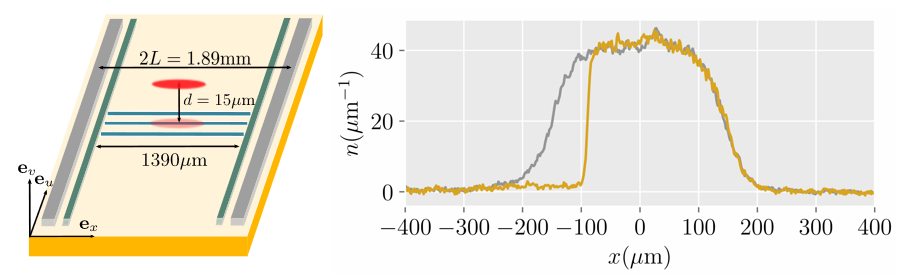
\includegraphics[width=0.9\linewidth]{figures/06_Bipart/Atom_chip.png}
%\caption{(a) Géométrie de la puce atomique. (b) Profils de densité longitudinale : en gris, gaz initial confiné dans un potentiel quartique ; en jaune, après illumination sélective et $1$~ms d’expansion libre.}
%\label{fig:setup}
%\end{figure}




\subsection{Cadre de la GHD et dynamique balistique et }
\label{sec.GHDpredictions}\label{sec:ghd}\label{chap6:sec:ghd}

{\color{blue}
Points clés :
\begin{itemize}
	\item Présentation du facteur d’occupation $\nu(x,\theta;t)$ comme variable hydrodynamique.
	\item Formulation de l’équation convective de GHD.
	\item Structure auto-similaire $\nu(x,\theta;t) = \nu^*(x/t,\theta)$ et résolution implicite via la vitesse effective.
	\item Prédictions analytiques pour le profil de densité $n(x,t)$.
\end{itemize}
}


Dans cette section, nous présentons le cadre théorique de la \emph{Théorie Hydrodynamique Généralisée} (GHD) appliqué à l’expérience décrite précédemment. L’objectif est de décrire analytiquement la dynamique balistique induite par une coupure bipartite dans un gaz quantique unidimensionnel, en exploitant les équations de GHD appliquées au modèle de Lieb-Liniger.\\

{\color{blue}
Nous procédons en plusieurs étapes : 
\begin{enumerate}
  \item Nous introduisons la description hydrodynamique à l’échelle d’Euler.
  \item Nous formulons les équations de GHD pour l’évolution du facteur d’occupation $\nu(x,\theta;t)$.
  \item Nous analysons la structure auto-similaire de la solution en régime hydrodynamique.
  \item Nous présentons la solution semi-analytique du problème de Riemann bipartite, ainsi que sa résolution graphique.
\end{enumerate}
}

\paragraph{Description hydrodynamique à l’échelle d’Euler}

Dans un système intégrable, les états stationnaires sont entièrement caractérisés par leur distribution de rapidités $\rho(\theta)$ ou, de manière équivalente, par le facteur d’occupation $\nu(\theta)$ (Cf {Chap~(\ref{chap:GHD})}). En régime hors équilibre, on suppose qu’à des échelles de temps longues et d’espace macroscopiques, le système évolue lentement vers un état localement stationnaire. Cela permet d’introduire une description hydrodynamique dans laquelle les quantités locales dépendent de la position et du temps : $\rho(x,\theta;t)$ ou $\nu(x,\theta;t)$.

%La densité linéique atomique est obtenue à partir de la distribution de rapidités par :
%\begin{equation}
%    n(x;t) = \int d\theta \, \rho(x,\theta ; t).
%    \label{eq:lineardensity}
%\end{equation}

\paragraph{Pourquoi travailler avec $\nu$ plutôt qu’avec $\rho$~?}
\subparagraph{Équation de GHD en termes de $\rho$.}
L’évolution à grande échelle du système est gouvernée par les équations de GHD~\cite{bertini_transport_2016, castro-alvaredo_emergent_2016}. 
L'évolution pour la distribution des rapidités $\rho(x,\theta;t)$ (Eq~\eqref{chap:GHD:eq.conserv.3.1}), en l'absence de potentiel extérieur, prend la forme d’une équation convective :
\begin{equation}
	\label{eq:rho.cont}
	\partial_t \rho + \partial_x \big( v^{\rm eff}_{[\rho]} \rho \big) = 0,
\end{equation}
où $v^{\rm eff}_{[\rho]}(\theta)$ est la vitesse effective des quasi-particules de rapidité $\theta$, fonctionnelle non linéaire de $\rho$ et où un terme de compression $\partial_x (v^{\rm eff}_{[\rho]} \rho)$ apparaît lorsqu’on développe la dérivée. Cela complique l’analyse, notamment lorsque les vitesses effectives varient fortement dans l’espace ou le temps.

Pour chaque rapidité $\theta$, l'équation \eqref{eq:rho.cont} constitue un cas particulier du problème de Riemann généralisé~\eqref{chap6:eq.Rieman.1}.
Nous considérons ici une condition initiale de type « coupure bipartite », représentant un état homogène à droite ($x>0$) et vide à gauche ($x<0$) :
\begin{equation}
    \label{eq:rho.cont.init}
    \rho(x,\theta;t=0) = 
    \begin{cases}
        \rho_0(\theta) & \text{si } x > 0, \\
        0 & \text{si } x < 0.
    \end{cases}
\end{equation}
Ce type de condition correspond , pour chaque rapidité $\theta$ , au condition introduit dans l'introduction \eqref{chap6:eq.Rieman.cond.1}.\\

\subparagraph{Équation de GHD en termes de $\nu$.}
En comparaison, l’évolution du facteur d'occupation $\nu(x,\theta;t)$ (Eq~\eqref{chap:GHD:eq.nu.1}) , qui, en l’absence de potentiel extérieur suit une équation de transport pur :
\begin{equation}
    \label{eq:nu.cont}
    \partial_t \nu + v^{\rm eff}_{[\nu]} \, \partial_x \nu = 0,
\end{equation}
où la dérivée temporelle est directement couplée à une dérivée spatiale. Cette forme préserve l'information le long des caractéristiques associées aux vitesses effectives $v^{\rm eff}_{[\nu]}$, ce qui rend la dynamique plus lisible et plus simple à analyser.

Les équation de transport pur \eqref{eq:nu.cont} ne sont pas  des cas particuliers du problème de Riemann généralisé~\eqref{chap6:eq.Rieman.1}. Et donc même si les conditions initials de type  « coupure bipartite » , pour $\nu$ :
\begin{equation}
    \label{eq:nu.cont.init}
    \nu(x,\theta;t=0) = 
    \begin{cases}
        \nu_0(\theta) & \text{si } x > 0, \\
        0 & \text{si } x < 0.
    \end{cases}
\end{equation}
sont du type \eqref{chap6:eq.Rieman.cond.1}.%, contrairement à \eqref{eq:rho.cont}, l'evolution \eqref{eq:nu.cont} ne génère pas de {\bf chocs}.\\

\medskip

Dans ce travail, nous choisissons de formuler la dynamique hydrodynamique généralisée en termes de la fonction d’occupation $\nu(x,\theta;t)$, plutôt que de la densité de quasi-particules $\rho(x,\theta,t)$. Cette approche présente plusieurs avantages. D’une part, l’équation vérifiée par $\nu$ est une équation de transport pur \eqref{eq:nu.cont}, ce qui permet une résolution naturelle par la méthode des caractéristiques, plus simplement que dans \eqref{eq:rho.cont}. D’autre part, $\nu$ possède une interprétation physique claire comme taux de remplissage des états accessibles, borné entre 0 et 1, ce qui en fait une variable plus stable et mieux adaptée aux calculs analytiques ou numériques.
De plus, la dynamique effective des observables s’exprime naturellement en fonction de $\nu$.
Enfin, $\nu$ et $\rho$ étant liés (par \eqref{eq:TBA-nu}), résoudre l’équation en $\nu$ revient, une fois $v^{\rm eff}_{[\nu]}$ déterminé, à résoudre complètement la dynamique de $\rho$.

\paragraph{Structure auto-similaire de la solution.}
Un point central est que les conditions initiales ~\eqref{eq:nu.cont.init} sont invariantes par dilatation. En effet quelque soit $\alpha >0$ , et pour tout $x$ réelle, on a $\nu(\alpha x , \theta ; t = 0 ) = \nu( x , \theta ; t = 0 ) $.
Un autre point central de la GHD est l’invariance d’échelle des solutions de l’équation~\eqref{eq:nu.cont} ( \eqref{eq:rho.cont} aussi et plus généralement de \eqref{chap6:eq.Rieman.1}) . En effet, si $\nu(x,\theta;t)$ est solution de  l’équation~\eqref{eq:nu.cont}, alors $\nu(\alpha x, \theta; \alpha t)$ l’est également ,  pour tout $\alpha > 0$ , avec les conditions initiales $\nu(\alpha x , \theta ; t = 0 )$. {\color{blue} Comme les fonctions $\nu(\alpha \cdot , \theta ; t = 0 )$ et $\nu( \alpha x , \theta ; t = 0 )$ coïncident, alors si $\eqref{eq:nu.cont}$ admet au plus une solution physique (entropique Cf Annex ~\ref{chap6:annex.Rieman}) pour chaque données initiales, on doit avoir $\nu( \alpha x , \theta ; \alpha t ) = \nu(  x , \theta ;  t )$ pour tout $\alpha > 0 $}. Sous hypothèse d’unicité (Cf Annex ~(\ref{chap6:annex.Rieman})), cette propriété implique que :
\begin{equation}
    \nu(x,\theta;t) = \nu^*\left(\frac{x}{t},\theta\right),
    \label{eq:nuvsnuetoile}
\end{equation}
autrement dit, les solutions dépendent uniquement du rapport $\xi = x/t$, appelé \emph{variable auto-similaire}. 


\paragraph{Résolution de l'évolution de $\nu$.} La dynamique est alors entièrement encodée dans la fonction $\nu^*(\xi,\theta)$, qui décrit la structure locale du gaz le long des rayons de vitesse $\xi$. Et,  pour $\xi$ est fixé, $\theta$  libre, \eqref{eq:nu.cont},  se réécrit  , avec des dérivés selon $\xi$ : 
\begin{equation}
	( \xi - v^{\rm eff}_{[\nu^\ast(\xi,\cdot )  ]}(\theta) )\, \partial_\xi \nu^\ast  = 0 .	
\end{equation}

Soit simplement pour chaque $\theta$, soit la vitesse effective est égale à $\xi$, soit $\partial_\xi \nu^\ast(\xi,\theta) = 0$.
%\begin{equation}
%	\partial_\xi \nu^\ast(\xi,\theta) = 0 , \quad \mbox{soit}\, 	
%\end{equation}


Autrement dit : pour une $\theta$ donnée, {\bf la fonction $\nu^\ast(\xi,\theta)$ est constante} en $\xi$, sauf au point $\xi = v^{\rm eff}_{[\nu^\ast(\xi , \cdot ) ]}(\theta)$, où une {\bf discontinuité} apparait.
%Cette équation admet deux types de solutions~: soit pour tout $\theta$ on a $\partial_\xi \nu^* = 0$, auquel cas $\nu^*$ est constante, ce qui correspond à un état homogène sans évolution intéressante ; soit pour tout $\theta$
%\begin{equation}
%	v^{\rm eff}_{[\nu^\ast(\xi, )]} = \xi	,
%\end{equation}
%qui définit implicitement la structure spatiale de la solution non triviale, en reliant chaque rayon $v$ à la vitesse effective locale.


La vitesse effective, $v^{\rm eff}{[\nu^\ast(\xi , \cdot ) ]}(\theta)$, est strictement monotone en $\theta$ ; il existe donc au plus un unique point $\theta^\ast$ tel que $\xi = v^{\rm eff}{[\nu^\ast]}(\theta^\ast)$, c’est-à-dire une seule discontinuité dans la solution.

La solution $\nu^*(\xi,\theta)$ s’écrit comme une fonction en escalier paramétrée par une valeur de coupure $\theta^*$ :
\begin{equation}
    \label{eq:nuetoile}
    \nu^*(\xi,\theta) = 
    \begin{cases}
        \nu_0(\theta) & \text{si } \theta < \theta^*, \\
        0 & \text{si } \theta > \theta^*,
    \end{cases}
    \quad \text{où on rappelle } v^{\rm eff}_{[\nu^*(\xi,\cdot)]}(\theta^*) = \xi.
\end{equation}
Cette équation implicite peut être résolue numériquement afin d'obtenir $\theta^*$ pour chaque valeur de $\xi$. On en déduit ensuite $\nu^*(\xi,\theta)$, puis $\rho(x,\theta;t)$ via les équations~\eqref{eq:TBA-rhos-2} et \eqref{eq:TBA-nu}, ce qui permet finalement de déterminer le profil de densité linéaire $n(x,t)$ à un instant donné : 
\begin{equation}
    n(x;t) = \int d\theta \, \rho(x,\theta ; t).
    \label{chap6:eq:lineardensity}
\end{equation}


\paragraph{Résumé}

Ainsi, dans le cadre de la GHD, la dynamique balistique résultant du quench bipartite est décrite par une solution auto-similaire paramétrée par une coupure en rapidité $\theta^*(\xi)$. Cette solution permet de prédire les profils de densité et d’occupation mesurables dans l’expérience. Elle fournit également un point de comparaison direct avec les données expérimentales obtenues à différents temps $t$, comme nous le verrons dans les sections suivantes.

\subsection{Validation expérimentale de la dynamique hydrodynamique}
\label{sec.don_exp}

%{\color{blue}
%Points clés :
%\begin{itemize}
%	\item Observation directe des profils $n(x,t)$ à différents temps.
%	\item Mise en évidence de l’auto-similarité en $x/t$ dans un régime temporel intermédiaire.
%	\item Comparaison quantitative avec la solution de GHD à température nulle.
%\end{itemize}
%}


Dans cette section, nous présentons les résultats expérimentaux obtenus après la coupure bipartite, et les comparons aux prédictions de la GHD à l’échelle d’Euler. L’objectif est de vérifier que la dynamique du gaz est bien décrite, à court et moyen terme, par une solution auto-similaire des équations hydrodynamiques.

%{\color{blue}
%Nous structurons cette analyse en quatre étapes :
%\begin{enumerate}
%    \item Description du protocole expérimental de libération.
%    \item Mise en évidence d’une structure auto-similaire.
%    \item Délimitation du domaine de validité temporelle de la GHD.
%    \item Comparaison quantitative avec la solution théorique à température nulle.
%\end{enumerate}
%}

\paragraph{Libération du gaz et expansion balistique.}

À l’issue du protocole de coupure décrit en sous-section~\ref{chap6:sec.propcol}, le confinement longitudinal est entièrement supprimé, tandis que le confinement transverse est maintenu. Cette opération permet au gaz de s’étendre librement le long de l’axe longitudinal, tout en conservant un comportement unidimensionnel (cf. section~\ref{sec:confinement}).
L’évolution du profil de densité $n(x,t)$ est alors enregistrée à différents temps $t$ après la libération, en utilisant une imagerie par absorption.


\paragraph{Mise en évidence de l’auto-similarité (régime d’Euler).}
Pour se concentrer sur les facteurs d'occupation $\nu$, on note simplement que la distribution de rapidité $\rho$ adopte une forme auto-similaire :
\(
\rho(x,\theta;t) = \rho^\ast(\xi,\theta),
\)
avec $\xi = x/t$.
En injectant dans l'equation~\eqref{chap6:eq:lineardensity}, il vient que dans le cadre de la GHD à l’échelle d’Euler, il est attendu que les profils de densité présentent une forme auto-similaire :
\begin{equation}
	n(x;t) = n^\ast\left( \xi \right),
\end{equation}
où $n^\ast$ ne dépend que de $\xi$.

\medskip

Cette propriété est testée expérimentalement en superposant les profils mesurés à différents temps, après mise à l’échelle selon $\xi = x/t$. La Fig.~\ref{fig:euler}(a) montre les profils normalisés mesurés entre $t = 10$~ms et $t = 18$~ms. L’excellent recouvrement obtenu confirme la validité du régime balistique et la pertinence de la description auto-similaire prédite par la GHD.

\paragraph{Contrainte experimentalles.}

La description par la GHD à l’échelle d’Euler est limitée à un domaine temporel intermédiaire $t \in [t_m, t_M]$ :

\begin{itemize}[label = $\bullet$]
  \item Pour $t > t_M \simeq 18$~ms, la densité maximale du gaz devient trop faible, et les effets de taille finie altèrent la validité de l’approximation d’un système semi-infini.
  \item Pour $t < t_m \simeq 6 \pm 2$~ms, plusieurs effets remettent en question la validité de la GHD :
  \begin{itemize}[label = $\circ$]
    \item La coupure initiale n’est pas parfaitement abrupte (longueur caractéristique $\sim 1~\mu$m).
    \item La résolution de l’imagerie limite la détection fine du bord.
    \item La GHD n’est valable qu’aux grandes échelles spatio-temporelles.
  \end{itemize}
\end{itemize}

Ainsi, dans nos conditions expérimentales, le régime GHD est atteint de manière fiable pour des temps compris entre $t_m \approx 6$~ms et $t_M \approx 18$~ms.

%\paragraph{Comparaison avec la prédiction théorique à température nulle.}
%
%Une fois la structure auto-similaire établie, il est possible de comparer directement les données expérimentales avec la prédiction théorique de la GHD dans le régime de quasi-condensat à température nulle. Cette limite correspond à une solution exacte de l’équation~\eqref{eq:GPE}, avec un paramètre de Lieb $\gamma \ll 1$.
%
%La Fig.~\ref{fig:euler}(b) présente une telle comparaison pour $t = 10$~ms et $\gamma = 4{,}6 \times 10^{-3}$. On observe une bonne correspondance entre le profil mesuré et la prédiction théorique, confirmant que la dynamique observée est bien capturée par la GHD dans cette limite.

\begin{figure}[!htb]
\centering
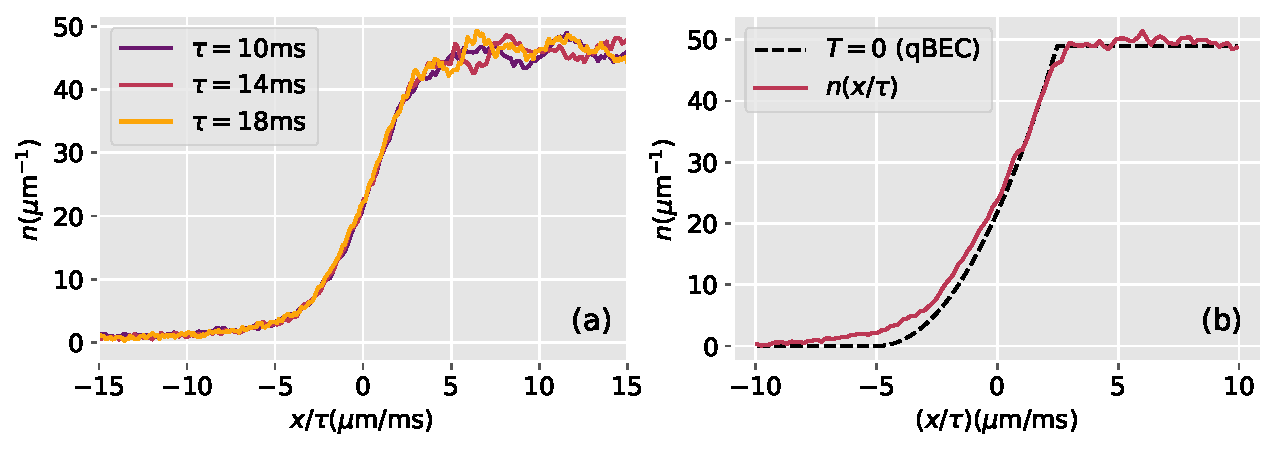
\includegraphics[width=1.0\linewidth]{figures/06_Bipart/DWD_GPE_vs_exp_V2.pdf}
\caption{
(a) Profils de densité mesurés pour différents temps $t$, représentés en fonction de la variable $x/t$. L’excellent recouvrement des courbes confirme l’auto-similarité et la dynamique balistique.\\
(b) Comparaison entre un profil mesuré à $t = 10$~ms (points) et la prédiction GHD à température nulle (ligne), pour un paramètre de Lieb $\gamma = 4{,}6 \times 10^{-3}$.
}
\label{fig:euler}
\end{figure}

\paragraph{Conclusion}

Ces observations expérimentales confirment que la dynamique induite par une coupure bipartite est bien décrite par la GHD à l’échelle d’Euler, dans un régime temporel intermédiaire bien identifié. La mise à l’échelle en $x/t$ permet une confrontation directe entre théorie et expérience, et ouvre la voie à des tests plus précis des effets thermiques et des corrections hors-échelle d’Euler.

\subsection*{Résumé}

Nous avons étudié la dynamique hors équilibre d’un gaz unidimensionnel de bosons à la suite d’une coupure bipartite, créant une discontinuité initiale dans le profil de densité. Cette configuration, analogue au problème de Riemann quantique, engendre une évolution balistique décrite par la Théorie Hydrodynamique Généralisée (GHD).

Sur le plan expérimental, nous avons mis en œuvre un protocole précis pour préparer un gaz homogène, le scinder spatialement à l’aide d’un DMD, puis le libérer dans un guide unidimensionnel. L’évolution du profil de densité $n(x,t)$ a été mesurée pour différents temps, révélant une structure auto-similaire caractéristique du régime hydrodynamique.

Côté théorique, nous avons présenté les équations de GHD dans leur forme convective, et montré que la solution du problème de Riemann s’exprime sous la forme d’une distribution auto-similaire $\nu(x/t, \theta)$. Cette structure permet de prédire analytiquement les profils de densité.

La comparaison entre les données expérimentales et les prédictions de la GHD à température nulle montre une excellente correspondance dans un régime temporel intermédiaire bien défini ($t \in [6,18]$~ms). Ces résultats valident la GHD comme cadre pertinent pour décrire la relaxation balistique de systèmes quantiques intégrables, et ouvrent la voie à des explorations plus fines des effets thermiques et quantiques hors équilibre.



\section{Sonder la distribution locale des rapidités}
\label{sec:local}

%{\color{blue}
%Points clés :
%\begin{itemize}
%	\item Protocole expérimental pour extraire une tranche locale du gaz après évolution.
%	\item Expansion 1D de la tranche sélectionnée et reconstruction de la distribution de rapidités $\Pi(\theta)$.
%	\item Comparaison avec les prédictions GHD : asymétrie, effet de la largeur finie de la tranche, et limitations dues à la résolution et aux effets diffusifs.
%	\item Discussion sur les écarts observés et les hypothèses du modèle.
%\end{itemize}
%
%}


\subsection*{Introduction}
Les outils de l'hydrodynamique généralisée (GHD) introduits dans la section~\ref{chap6:sec:ghd} permettent de décrire la dynamique hors équilibre dans des configurations de type jonction bipartite.
Dans le scénario de jonction bipartite — où deux parties du gaz, initialement préparées dans des états thermodynamiques distincts, sont soudainement mises en contact — la dynamique engendre des profils locaux fortement hors équilibre. En particulier, lorsque l’état initial consiste en un gaz homogène à droite et une région vide à gauche, la GHD prédit qu’à grand temps le système atteint un régime stationnaire autosimilaire, dans lequel les observables locales dépendent uniquement du {\em variable auto-similaire} $\xi = x/t$. Dans ce régime, la distribution locale des quasi-particules est décrite par un facteur d’occupation $\nu^*(\xi,\theta)$, solution d’une équation de type~\eqref{eq:nuetoile}.

\medskip

Une prédiction remarquable de ce cadre est la présence, du côté droit du système, d’une discontinuité abrupte dans la distribution en rapidité du facteur d’occupation~$\nu^*(\xi,\theta)$ — signature d’un état local proche du fondamental. À l’inverse, du côté gauche (où le gaz est initialement absent), la distribution reste lisse en rapidité, ce qui indique un état localement excité, distinct d’un état fondamental. Ce contraste fort entre les deux régions — l’une présentant une distribution lisse, l’autre une discontinuité abrupte — reflète la propagation balistique des quasi-particules, conséquence directe de l’intégrabilité du système. En effet, dans un système intégrable, les quasi-particules conservent leur individualité et se propagent à vitesse bien définie sans diffusion, ce qui permet de maintenir à grand temps des structures non thermalisées comme des discontinuités, absentes dans les systèmes non intégrables.

\medskip

L’objectif de cette section est de confronter ces prédictions théoriques à l’expérience, en accédant à la distribution locale de rapidités du gaz. Pour cela, nous mettons en œuvre un protocole expérimental inspiré de la Réf.~\cite{dubois_probing_2024}, permettant de mesurer indirectement cette distribution via l’expansion libre d’une tranche localisée du gaz. En parallèle, nous réalisons des simulations numériques de la dynamique à l’aide de la GHD, ce qui nous permet de comparer les distributions mesurées avec les prédictions théoriques, et ainsi de tester la présence effective de la discontinuité attendue.

\medskip

%{\color{blue}
%Nous structurons cette analyse en quatre étapes principales :
%\begin{itemize}
%    \item Sélection d’une tranche localisée du gaz après un temps d’évolution donné.
%    \item Observation du profil de vitesse après expansion libre, révélant une éventuelle asymétrie.
%\end{itemize}
%}

\begin{figure}[!htb]
\centering
\begin{tikzpicture}
    \node[rectangle, draw = none] (bord) at (0,0) {
        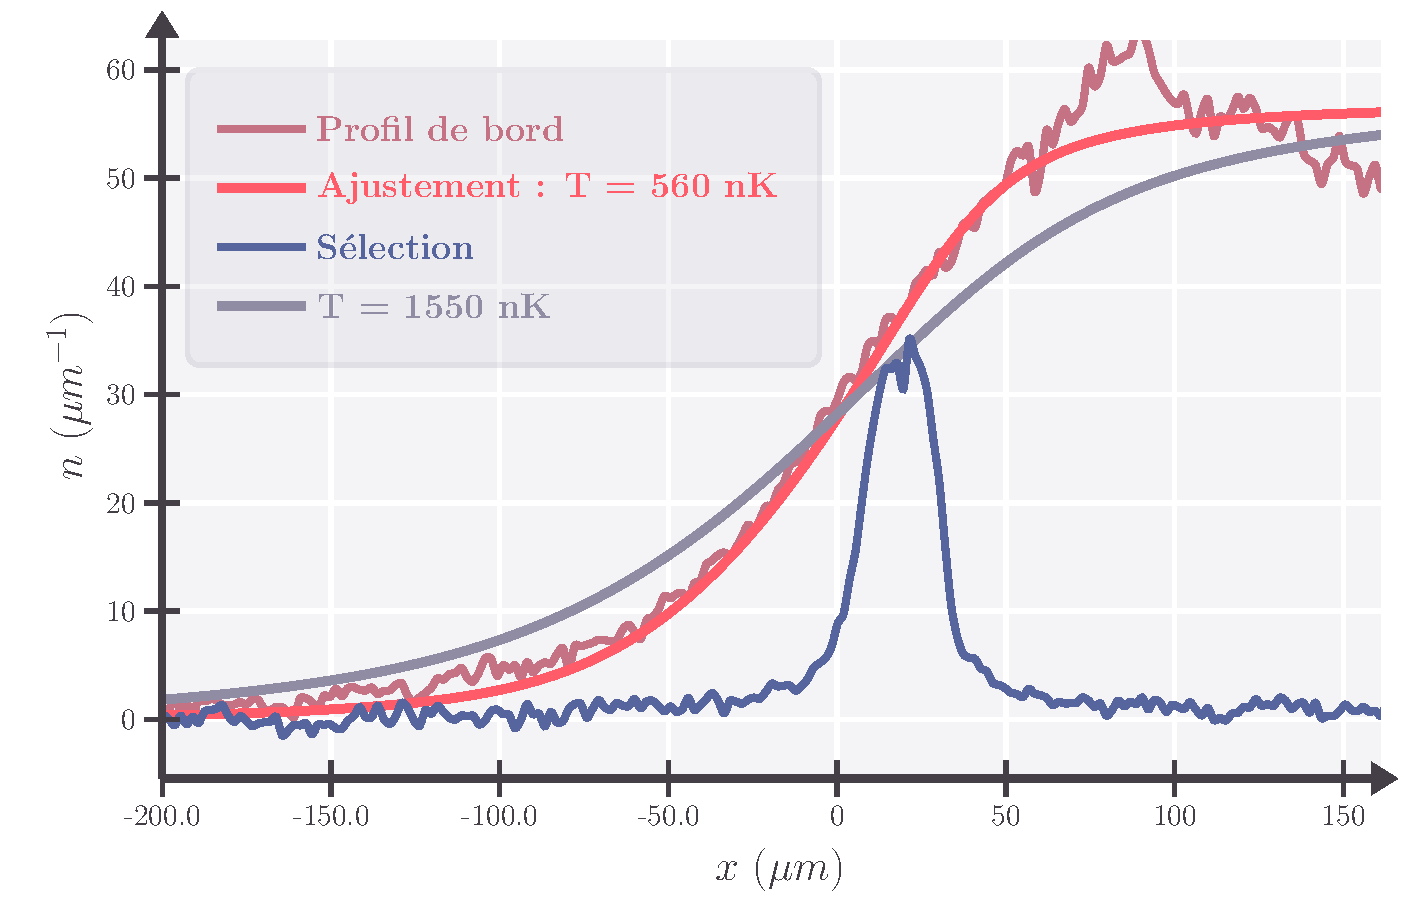
\includegraphics[width=0.5\textwidth , page = 1]{figures/06_Bipart/Figures}
    };
    \node[circle, draw=none, above=0cm of bord , shift={( -2.5cm , -0.5cm )} ] {(a)};
    
    \node[right=1mm of bord , shift={( -0.5cm , 0cm )}] (assy) {
        \includegraphics[width=0.5\textwidth , page = 2 ]{figures/06_Bipart/Figures}
    };
    \node[circle, draw=none, above=0cm of assy , shift={( -2.5cm , -0.5cm )}] {(b)};
\end{tikzpicture}
\caption{(a) {\it Profil de bord et tranche sélectionnée.} Le profil de bord après $18\,\mathrm{ms}$ est montré en rouge. L'ajustement thermique donne une température $T = 560\,\mathrm{nK}$ (orange). Le profil de densité mesuré $1\,\mathrm{ms}$ après la sélection de la tranche est en bleu. (b) {\it Asymétrie du profil d’expansion de la tranche.} Le profil de densité après une expansion pendant $\tau = 30\,\mathrm{ms}$ est comparé à son image miroir. Le centre de symétrie $x_s = -17\,\mu$m minimise la distance quadratique $\delta^2 = \int dx\, (\tilde{n}(x) - \tilde{n}(2x_s - x))^2$.}
\label{fig:simul_deformation}
\end{figure}



%\subsection{Protocol experimental}

\subsection{Sélection d’une tranche localisée après déformation du bord}

%{\color{blue}
%Nous laissons d’abord le gaz se dilater pendant un temps $t=18~\mathrm{ms}$, de sorte que le bord s’étale sur une large zone d’environ $350~\mathrm{\mu m}$, comme illustré en Fig.~\ref{fig:BiPart.coupure1} (e)-(f) et  Fig ~\ref{fig:simul_deformation} (a).  
%Nous sélectionnons ensuite une tranche du gaz comprise dans l’intervalle $[x_0-\ell/2, x_0+\ell/2]$, en éliminant tous les atomes situés hors de cette tranche à l’aide d’un faisceau pousseur~\cite{dubois_probing_2024}(Fig \ref{fig:BiPart.coupure2} (a)--(c)). 
% 
%
%}


\paragraph{Sélection locale d'une tranche du gaz.}

Afin d’accéder localement à la distribution de rapidité, nous exploitons le fait qu’après un temps $t = 18~\mathrm{ms}$, le bord du gaz s’étale sur plusieurs centaines de microns — environ $350~\mathrm{\mu m}$ — comme illustré en Fig.~\ref{fig:BiPart.coupure1}(e)-(f) et Fig.~\ref{fig:simul_deformation}(a). Cette large extension spatiale permet d’identifier des régions à la fois assez étendues pour être sélectionnées expérimentalement, et suffisamment étroites pour que le gaz puisse y être considéré comme localement homogène dans le cadre de l’hydrodynamique généralisée.

\medskip
\noindent
Pour isoler une telle région, un {\bf faisceau pousseur} est appliqué afin d’{\bf éliminer tous les atomes situés hors d’un intervalle spatial} centré en $x_0 = 18~\mu\mathrm{m}$ et de largeur $\ell$. Cette technique, inspirée de la Réf.~\cite{dubois_probing_2024}, permet de ne conserver qu’une {\bf tranche localisée du gaz}, dont la distribution en rapidité reflète l’état local $\rho(x,\theta)$ aux abords de $x \approx x_0$, comme illustré en Fig.~\ref{fig:BiPart.coupure2}(a)--(c).


\medskip
\paragraph{Contrôle expérimental du faisceau de sélection.}

La sélection spatiale du gaz est réalisée à l’aide d’un dispositif à micro-miroirs (DMD), qui permet de contrôler finement la forme du faisceau pousseur utilisé pour éliminer les atomes hors d’un intervalle centré en $x_0$. Ce dispositif est piloté via une interface logicielle développée au sein de l’équipe, basée sur les outils \textsc{Cicero-Iso} et \textsc{Spartacus}. Le DMD est commandé par une série de paramètres expérimentaux transmis à ces logiciels, dont certains (comme la position $x_0$) sont enregistrés systématiquement au cours de l’expérience. En revanche, d'autres paramètres, notamment la largeur effective $\ell$ du faisceau, n’ont pas été archivés dans la base de données associée aux séquences expérimentales. Ainsi, dans les paragraphes précédents, nous avons pu indiquer précisément la valeur de $x_0$ (ici $x_0 = 18~\mu\mathrm{m}$), mais non celle de $\ell$. Cette valeur sera déterminée a posteriori par analyse des profils expérimentaux, et jouera un rôle essentiel dans les simulations numériques présentées plus loin.

\medskip
\paragraph{Inhomogénéité de la tranche sélectionnée}

Dans l'idéal, on souhaiterait que l’intervalle de sélection soit suffisamment fin pour garantir l’homogénéité de la densité locale au sein de la tranche. Toutefois, comme la valeur exacte de $\ell$ n’a pas été enregistrée, nous ne pouvons pas l’estimer directement à partir des données de Fig.~\ref{fig:simul_deformation}(a), qui représente l’état du système avant sélection. Néanmoins, cette même figure montre également le profil de densité mesuré une milliseconde après la sélection. Or, comme nous le verrons dans la suite, les simulations GHD montrent que, dans cet intervalle de temps, la distribution en espace réel ne subit ni déplacement significatif, ni déformation notable. Il est donc raisonnable d’utiliser ce profil post-sélection comme estimation fidèle de la densité initiale dans la tranche.

\medskip
\paragraph{Estimation de la largeur $\ell$ et conséquences}

À partir de cette analyse, nous pouvons estimer que la largeur $\ell$ de la tranche sélectionnée est de l’ordre de $20$ à $30~\mu\mathrm{m}$. Or, pour une position centrale $x_0 \approx 18~\mu\mathrm{m}$, la densité atomique $\tilde{n}(x ; \tau = 0 )$ varie sensiblement sur cette échelle. La tranche sélectionnée n’est donc pas localement homogène, et la distribution de rapidité mesurée correspond en réalité à une moyenne spatiale de $\rho(x,\theta)$ sur un intervalle de largeur $\ell$ centré en $x_0$. Cette observation est essentielle pour l’interprétation des données et sera prise en compte dans la suite, en particulier dans les comparaisons avec les simulations hydrodynamiques.


\subsection{Expansion de la tranche et observation d’une asymétrie}

\paragraph{Principe de l’expansion et lien avec la distribution en rapidité}

Après la sélection, la tranche est laissée en expansion libre unidimensionnelle pendant un temps $\tau$, puis son profil de densité longitudinal $\tilde{n}(x,\tau)$ est mesuré. Cette expansion permet de convertir l’information spatiale en une information sur la distribution en rapidité. En effet, pour un temps $\tau$ suffisamment grand, on s’attend à ce que la densité observée soit proportionnelle à la distribution totale des rapidités dans la tranche :
\begin{equation}
\tau\, \tilde{n}(\tau \theta - x_0 ; \tau) \underset{\tau \to \infty}{\longrightarrow} \Pi(\theta),
\end{equation}
où, quel que soit le temps d'expansion unidimensionnelle $\tau$, la distribution de rapidité extensive $\Pi(\theta)$ reste constante, c’est-à-dire  $\Pi(\theta) = \int \rho(x, \theta ; \tau \geq 0)\, dx $. En particulier, cette distribution s’identifie à celle de l’état initial dans la tranche sélectionnée :
\begin{equation}
\Pi(\theta)  = \int_{x_0 - \ell/2}^{x_0 + \ell/2} \rho(x, \theta ; \tau = 0)\, dx.
\end{equation}
Autrement dit, $\Pi(\theta)$ correspond à la distribution de rapidité intégrée sur la tranche sélectionnée, conservée lors de l’expansion.

\paragraph{Observation expérimentale de l’asymétrie}

La théorie prédit que la distribution locale de quasi-particules $\rho(x,\theta)$ est fortement asymétrique en $\theta$. Cette asymétrie se retrouve dans $\Pi(\theta)$ et doit donc se manifester dans le profil d’expansion $\tilde{n}(x,\tau)$. Cette asymétrie est effectivement observée dans nos données expérimentales, comme illustré en Fig.~\ref{fig:simul_deformation}(b) pour un temps d’expansion $\tau = 30~\mathrm{ms}$. 


\subparagraph{Quantification de l’asymétrie par symétrisation.}
La figure \ref{fig:simul_deformation}(b) présente deux courbes : le profil mesuré $\tilde{n}(x)$ (abréviation de $\tilde{n}(x,\tau)$) et son image par symétrie par rapport à un axe $x = 2x_s$. L’objectif est de rendre visible et de quantifier l’asymétrie du profil.
Pour ce faire, nous considérons une décomposition naturelle du profil autour d’un centre $x = x_s$ :
\begin{equation}
\tilde{n}(x) = \tilde{n}_{\text{pair}}^{(x_s)}(x) + \tilde{n}_{\text{impair}}^{(x_s)}(x),\quad \mbox{où} \, \left\{\begin{array}{lcr}\tilde{n}_{\text{pair}}^{(x_s)}(x) &=&  \displaystyle \frac{\tilde{n}(x) + \tilde{n}(2x_s - x)}{2} , \\ \tilde{n}_{\text{impair}}^{(x_s)}(x) &=& \displaystyle \frac{\tilde{n}(x) - \tilde{n}(2x_s - x) }{2}\end{array} \right. .
\end{equation}

Cette décomposition correspond à une projection du profil sur les fonctions paires et impaires centrées en $x = x_s$.

L’asymétrie du profil est directement liée à la composante impaire. Pour la quantifier, nous cherchons la valeur de $x_s$ qui minimise la norme $L^2$ de la partie impaire :
\begin{equation}
\mathcal{\delta}^2(x_s) = \int dx\, \left[\tilde{n}(x) - \tilde{n}(2x_s - x)\right]^2.
\end{equation}
La valeur optimale de $x_s$ minimise cette fonctionnelle $\mathcal{\delta}^2(x_s)$ et fournit un axe de symétrie effectif pour le profil. Cette méthode permet de comparer de manière robuste différentes conditions expérimentales, ou différents temps d’expansion, en s’affranchissant d’un ajustement arbitraire de centre.


\subparagraph{Effet de l’homogénéité de la tranche sélectionnée}

Plus la densité atomique est homogène dans la tranche sélectionnée, plus l’expansion est asymétrique et restitue fidèlement la distribution de rapidité au point $x_0$. En effet, si $\rho(x,\theta)$ est uniforme sur la largeur $\ell$, on obtient :
\begin{equation}
\Pi(\theta) \simeq \ell\, \rho(x_0,\theta) \quad \Rightarrow \quad \tau\, \tilde{n}(\tau \theta - x_0 ; \tau) \simeq \ell\, \rho(x_0,\theta),
\end{equation}
ce qui permet d’accéder directement à la distribution locale, y compris à d’éventuelles discontinuités.

Deux stratégies permettent d’améliorer cette homogénéité :
\begin{itemize}[label = $\bullet$] 
    \item Diminuer la largeur $\ell$ de la sélection,
    \item Augmenter le temps $t$ de déformation du bord avant sélection, pour étendre la région d’intérêt spatialement.
\end{itemize}
Cependant, ces deux approches ont des limitations : une plus petite valeur de $\ell$ réduit le nombre d’atomes sélectionnés, ce qui diminue le rapport signal/bruit, et des temps $t$ trop longs font sortir le système du régime semi-infini, introduisant des effets de bord non désirés (voir Fig.~[à insérer]).

\subparagraph{Limites sur le temps d’expansion}

Allonger le temps d’expansion $\tau$ permet d’approcher plus fidèlement le régime asymptotique $\tau \to \infty$ où la correspondance avec $\Pi(\theta)$ est exacte. Toutefois, cette expansion est limitée expérimentalement par la taille longitudinale du confinement 1D, de l’ordre de $1~\mathrm{mm}$, correspondant à la taille typique des triplets de microfils. Comme illustré en Fig.~\ref{fig:simul_deformation}(b), le nuage atteint cette taille à $\tau \sim 30~\mathrm{ms}$, ce qui constitue une limite pratique. Par ailleurs, des simulations GHD (voir Ref.~\cite{dubois_probing_2024}) montrent que des temps significativement plus longs seraient nécessaires pour que $\tau \tilde{n}$ converge véritablement vers $\Pi(\theta)$.

\subparagraph{Renforcer l’asymétrie observée}

Enfin, une asymétrie plus marquée peut être obtenue en modifiant l’état initial du gaz. En particulier, une bipartition réalisée à partir d’un état initial plus excité (c’est-à-dire moins proche du fondamental) du côté gauche renforcerait le contraste entre les deux côtés. Cette stratégie permettrait d’amplifier la discontinuité attendue dans la distribution de rapidité, et donc dans le profil d’expansion.

\vspace{1em}
\begin{center}
\textit{[Figure : asymétries observées pour différents états initiaux]}
\end{center}

\subsection*{Résumé}

Dans cette section, nous avons présenté un protocole permettant de sonder la distribution locale des quasi-particules dans un gaz unidimensionnel hors équilibre, en sélectionnant une tranche étroite après déformation du bord, puis en la laissant s’étendre librement. Cette procédure permet d’accéder indirectement à la distribution intégrée en rapidité $\Pi(\theta)$ dans la tranche, et de tester les prédictions de la GHD sur la structure locale du facteur d’occupation $\nu(x,\theta)$.

L’analyse expérimentale révèle une forte asymétrie du profil d’expansion, signature d’une distribution de rapidité non thermique. La méthode de symétrisation introduite permet de quantifier cette asymétrie de manière robuste. Nous avons montré que l’homogénéité de la tranche sélectionnée, la durée d’expansion libre, ainsi que l’état initial du gaz influencent fortement l’observation de cette asymétrie.

Enfin, ces résultats confirment qualitativement les prédictions de la GHD dans le régime stationnaire autosimilaire, en particulier l’existence d’une discontinuité du côté du gaz initialement présent, tout en mettant en évidence les limitations expérimentales et les effets hors modèle — notamment les contraintes liées à la sélection spatiale et à la durée d’expansion.

\medskip

Pour approfondir cette analyse, nous nous appuyons à présent sur des simulations numériques basées sur l’équation de GHD. Celles-ci permettent de modéliser la dynamique complète de la tranche sélectionnée, depuis la déformation du bord jusqu’à son expansion, et de confronter quantitativement les distributions mesurées aux prédictions théoriques.


\section{Simulations numériques}
\label{sec:simulations}

Cette section présente en détail les étapes nécessaires à la résolution numérique de l’équation de GHD dans le cadre des simulations effectuées.

Dans un premier temps, nous explicitons le calcul du facteur d’occupation $\nu(\theta)$ et de la densité de rapidité $\rho(\theta)$ à l’équilibre thermique, obtenus à partir d’un couple $(T, \mu)$ donné.

Nous décrivons ensuite l’évolution du système sous l’effet du potentiel de piégeage : en particulier, nous nous intéressons à la dynamique du contour délimitant la région occupée dans l’espace des phases $(x, \theta)$, en exploitant la conservation lagrangienne du facteur d’occupation.

La simulation permet alors de suivre la déformation du bord au cours du temps. Une fois ce bord suffisamment évolué, nous extrayons une tranche du système pour en simuler l’expansion.

Enfin, nous comparons la distribution de rapidité issue de cette expansion numérique avec celle mesurée expérimentalement, dans des conditions analogues.


\subsection{Système homogène à l'équilibre thermique}

Nous considérons d’abord un gaz unidimensionnel homogène infini, à l’équilibre thermique, caractérisé par un couple de paramètres thermodynamiques $(T, \mu)$. La thermodynamique de Bethe-Ansatz permet de décrire un tel système par une équation intégrale sur le poids/potentiel spectral $w(\theta)$, donnée par :
\begin{equation}
w(\theta) = \beta\left(\frac{1}{2}m\theta^2 - \mu\right),
\end{equation}
où $\beta = (k_B T)^{-1}$ est l’inverse de la température (en unités d’énergie). La résolution de cette équation donne accès au facteur d’occupation $\nu_0(\theta)$ .

À partir de $\nu_0(\theta)$, les densités de quasi-particules $\rho(\theta)$ et de niveaux disponibles $\rho_s(\theta)$ sont obtenues par un processus de {\bf habillage} (ou {\bf dressing}) standard (voir section~\ref{para-algho-TBA}). Ces grandeurs sont ensuite utilisées pour calculer les observables physiques.



\paragraph{Détermination du potentiel chimique à température fixée}

Dans l’expérience, la quantité accessible est la densité linéique homogène $n_0$, par exemple $n_0 = 56~\mu\mathrm{m}^{-1}$ (voir Fig.~\ref{fig:simul_deformation}(a)). Afin de reproduire cette densité dans les simulations, nous fixons la température $T$ (déterminée indépendamment dans l’expérience), puis nous ajustons la valeur du potentiel chimique $\mu$ pour satisfaire la contrainte :
\begin{equation}
n_0 = \int \rho_0(\theta)\, d\theta.
\end{equation}

Ce processus est effectué numériquement en résolvant les équations TBA pour différentes valeurs de $\mu$ jusqu’à obtenir l’accord avec la densité cible. Dans notre cas, pour $T = 560~\mathrm{nK}$, nous obtenons $\mu = 65~\mathrm{nK}$ comme valeur correspondant à la densité $n_0 = 56~\mu\mathrm{m}^{-1}$.

Les résultats de cette résolution sont illustrés en Fig.~\ref{fig:BiPart.insitut} :
\begin{itemize}[label = $\bullet$]
    \item Le facteur d’occupation obtenu $\nu_0(\theta)$ est représenté en (a).
    \item La densité spatiale correspondante, constante dans le cas homogène, est illustrée en (b).
    \item Le facteur $\nu_0(\theta)$ est à nouveau tracé en (c), en complément pour lecture directe.
\end{itemize}

Dans ce régime homogène, la distribution est indépendante de la position, i.e.
\begin{equation}
\nu(x, \theta) = \nu_0(\theta), \quad \forall x,
\end{equation}
comme visible en Fig.~\ref{fig:BiPart.insitut}(a,c).


\begin{figure}[!htb]
	\centering
	\includegraphics[width=0.5\textwidth , page = 4 ]{figures/06_Bipart/Shema.pdf}	
	\caption{a) Facteur d’occupation initial $\nu(x, \theta) = \nu_0(\theta)$ correspondant à un état d’équilibre thermique à la température $T = 560~\mathrm{nK}$, pour une densité linéique homogène $n_0 = 56~\mu\mathrm{m}^{-1}$. Ces paramètres correspondent à une potentielle chimique $\mu = 65~\mathrm{nK}$.
b) Densité spatiale linéique $n(x) = \int \rho_{[\nu]}(x, \theta)\, d\theta$, constante et égale à $n_0 = 56~\mu\mathrm{m}^{-1}$.
c) Facteur d’occupation $\nu_0(\theta)$ correspondant à la distribution thermique illustrée en a).}
	\label{fig:BiPart.insitut}
\end{figure}


\subsection{Dynamique du contour dans l’espace des phases $(x, \theta)$.}
\label{sec:contour_GHD}

Une fois le facteur d’occupation initial $\nu_0(\theta)$ déterminé, nous cherchons à décrire l’évolution temporelle de la région occupée dans l’espace des phases $(x,\theta)$. Cette région, notée $\Gamma_t$, est définie comme le support du facteur d’occupation $\nu(x,\theta,t)$ : elle contient l’ensemble des points pour lesquels $\nu$ est non nul à l’instant $t$.

\paragraph{Interprétation lagrangienne et trajectoires caractéristiques :.}
Dans l’hydrodynamique généralisée, l’évolution de $\nu$ est décrite par une équation de transport pur du type \eqref{eq:nu.cont}. Cette équation peut être interprétée selon une perspective \textbf{lagrangienne} :  le facteur d’occupation $\nu$ reste constant au cours du temps c'est à dire  
\begin{eqnarray}\label{chap6:eq:traj_lagr_0}
	 \nu ( x(t) , \theta(t) ; t ) = \nu ( x(0) , \theta(0) ; 0 ) 
\end{eqnarray}
lorsqu’on suit les trajectoires $(x(t), \theta(t))$ définies par :  
\begin{eqnarray*}
	\frac{d \nu}{dt} (x , \theta ; t ) = 0,	
\end{eqnarray*}

soit $\partial_t \nu + \dot{x} \partial_t \nu = 0$ soit en identifiant dans \eqref{eq:nu.cont}:
\begin{equation}
\label{chap6:eq:traj_lagr_1}
\partial_t \left( \begin{array}{c} x(t) \\ \theta(t) \end{array} \right)  =  \left( \begin{array}{c} v^{\mathrm{eff}}_{[\nu]}(\theta(t)) \\ 0 \end{array} \right)\, \mbox{soit} \quad \left\{ \begin{array}{rcl}
\displaystyle \frac{d x}{dt}(t) & = & v^{\mathrm{eff}}_{[\nu]}(\theta), \\
\theta(t) & = & \theta(0) \equiv \theta.
\end{array} \right. 
\end{equation}
%où $s$ est un paramètre pour différentier les particules fluide dans la perspective lagrangienne. Cette dernière équation \eqref{chap6:eq:traj_lagr_1} implique que 
%\begin{equation}
%\label{chap6:eq:traj_lagr_2} 
%\left\{ \begin{array}{rcl}
%\displaystyle \frac{d x}{dt}(s;t) & = & v^{\mathrm{eff}}_{[\nu]}(\theta(s)), \\
%\theta(s;t) & = & \theta(s;0) = \text{constante}.
%\end{array} \right.
%\end{equation}

Autrement dit, les quasi-particules de rapidité $\theta$ se déplacent à la vitesse efficace $v^{\mathrm{eff}}_{[\nu]}$, et leur répartition reste inchangée tout au long de leur trajectoire dans l’espace des phases. Cette conservation est analogue à une conservation lagrangienne classique, où l’on suit un élément de fluide individuellement.

\medskip

\paragraph{État initial en "patch" et Propagation du support .}
Nous considérons un état initial de type « patch » : le facteur d’occupation $\nu(x ,\theta ;0)$ est égal à $\nu_0(\theta)$ à l’intérieur d’une certaine région initiale $\Gamma_0$, et nul en dehors. Ce choix modélise une situation typique de type « front d’onde » avec un gaz localement homogène dans une portion de l’espace.

En suivant chaque point $(x(t),\theta)$ de cette région selon l’équation~\eqref{chap6:eq:traj_lagr_1}, on détermine la région atteinte à l’instant $t$, notée $\Gamma_t$. Par construction, le facteur d’occupation reste constant le long de ces trajectoires d'après \eqref{chap6:eq:traj_lagr_0}, $\nu(x(t),\theta,t) = \nu(x(0),\theta,0)$  soit :

\begin{equation}
	\nu(x(t),\theta,t)  = \nu_0(\theta).
\end{equation}

Par conséquent, on peut écrire l’évolution du facteur d’occupation de manière explicite :

\begin{equation}
\label{eq:contour_support}
\nu(x, \theta, t) =
\begin{cases}
\nu_0(\theta) & \text{si } (x,\theta) \in \Gamma_t, \\
0 & \text{sinon}.
\end{cases}
\end{equation}

Cette propriété est une conséquence directe du cadre intégrable sous-jacent et de la forme particulière de l’équation de GHD, qui assure que les caractéristiques $(x(t),\theta)$ suivent une dynamique conservant localement l’occupation.

\medskip

Enfin, notons que, dans ce cadre, la vitesse efficace $v^{\mathrm{eff}}_{[\nu]}(x,\theta,t)$ est fonctionnelle du facteur d’occupation \textit{instantané}. Toutefois, dans les cas où $\nu$ conserve sa structure initiale par blocs (comme ici avec un contour net), on peut exprimer cette vitesse uniquement à partir de $\nu_0$ sur chaque trajectoire, ce qui permet de déterminer toute la dynamique sans recalculer le champ $\nu$ à chaque pas de temps. Cette remarque est à la base des méthodes numériques efficaces employées dans nos simulations (voir section~\ref{sec:simu_bord}).


\subsection{Simulation de la déformation du bord}

Dans la configuration initiale correspondant à l'expérience de déformation du bord (Fig.~\ref{fig:BiPart.coupure1}), la région occupée par le gaz correspond à \(x > 0\), avec un facteur d’occupation uniforme \(\nu(x,\theta; t=0) = \nu_0(\theta)\) pour \(x > 0\), et nul pour \(x < 0\). Le contour initial séparant ces deux domaines est donné par \((x = 0, \theta)\). L’évolution de ce front peut être entièrement décrite à l’aide de l’équation de GHD, en supposant que le contour reste bijectif au cours du temps.


Nous paramétrons ce contour par une variable \(s\), de sorte que le bord à l’instant \(t\) est donné par \((x_b(s;t), \theta_b(s))\), avec \(\theta_b(s)\) strictement croissante (i.e. \((x_b(s;t), \theta_b(s)) \in \partial \Gamma_t\)).  
La conservation lagrangienne du facteur d’occupation implique que la vitesse efficace \(v^{\mathrm{eff}}_{[\nu^\ast]}(\theta_b(s))\) est indépendante du temps de déformation \(t\).  
En dérivant \eqref{eq:traj_lagr}, on obtient que chaque point \((x_b(s;t), \theta_b(s))\) suit une trajectoire caractéristique associée à cette vitesse efficace :
\[
x_b(s;t) = v^{\mathrm{eff}}_{[\nu^\ast]}(\theta_b(s)) \cdot t,
\]
où \(\nu^\ast(v, \theta)\) désigne le facteur d’occupation exprimé dans les variables autosimilaires, avec \(v = x/t\).
Le facteur d’occupation autosimilaire prend alors la forme \eqref{eq:contour_support} :
\begin{equation}
\label{eq:contour_bord_sim}
\nu^\ast(x_b(s;t)/t,\theta)  =  	 \begin{cases} \nu_0(\theta) & \text{si }  \theta < \theta_b(s) \\ 0 & \text{sinon} \end{cases}, \, \quad \mbox{soit} \quad  	
\nu^\ast(v,\theta) = 
\begin{cases}
\nu_0(\theta) & \text{si }  v < v^{\mathrm{eff}}_{[\nu^\ast]}(\theta), \\
0 & \text{sinon} .
\end{cases}
\end{equation}
La vitesse efficace \(v^{\mathrm{eff}}_{[\nu^\ast]}(\theta)\) est déterminée par :
\(
v^{\mathrm{eff}}_{[\nu^\ast]}(\theta) = \frac{\mathrm{id}^{\mathrm{dr}}_{[\nu^\ast]}(\theta)}{\mathrm{1}^{\mathrm{dr}}_{[\nu^\ast]}(\theta)}.
\)
À partir de la connaissance du contour \((x_b(s;t), \theta_b(s))\), on reconstruit le facteur d’occupation \(\nu(x,\theta; t)\) à l’aide de l’équation~\eqref{eq:contour_bord_sim} (Fig. \ref{fig:BiPart.coupure1}~(e) $\&$(g)). On en déduit ensuite la densité totale de quasi-particules par :
\(
\rho_s(x,\theta;t) = \frac{\hbar}{m} \cdot 1^{\mathrm{dr}}_{[\nu]}(\theta),
\,
\rho(x,\theta;t) = \nu(x,\theta;t) \cdot \rho_s(x,\theta;t),
\)
puis la densité linéique :
\(
n(x,t) = \int \rho(x,\theta;t)\, d\theta.
\)
(Fig. \ref{fig:BiPart.coupure1}~(e)$\&$(f)).

\medskip 

Enfin, en fixant \(n_0 = 56~\mu\mathrm{m}^{-1}\), nous ajustons la température \(T\) des simulations GHD pour reproduire les données expérimentales de déformation du bord (Fig.~\ref{fig:simul_deformation}). Cet ajustement donne \(T = 560~\mathrm{nK}\).

\begin{figure}[!htb]
	\centering
	\includegraphics[width=\textwidth , page = 5 ]{figures/06_Bipart/Shema.pdf}
	\caption{
(a) À l'instant $t = 0^+$, immédiatement après le « quench bipartite » en $x = 0$, le facteur d'occupation est donné par $\nu(x, \theta ; t = 0^+) = \nu_0(\theta)$ pour $x > 0$ et est nul pour $x < 0$. Le bord initial représenté en tirets par l'ensemble des points $(x_b(s; t = 0^+) = 0,\ \theta(s; t = 0^+))$.
(b) Densité spatiale linéique $n(x)$ : en pointillés, $n(x; t = 0^-) = \int \rho(x, \theta; t = 0^-) \, \mathrm{d}\theta = n_0 = 56~\mu\mathrm{m}^{-1}$ juste avant le quench ; en ligne pleine, $n(x; t = 0^+) = n_0$ pour $x > 0$ et $0$ pour $x < 0$.
(c) À gauche de la coupure ($x < 0$) : en pointillés, $\nu(x, \theta ; t = 0^-) = \nu_0(\theta)$ ; en ligne pleine, $\nu(x, \theta ; t = 0^+) = 0$.
(d) À droite de la coupure ($x > 0$), le facteur d'occupation reste inchangé : $\nu(x, \theta ; t = 0^+) = \nu_0(\theta)$.
(e) À l'instant $t = 18~\mathrm{ms}$, après l'évolution balistique post-quench, le facteur d'occupation est donné par $\nu^\ast(x_b(s;t)/t, \theta) = \nu_0(\theta)$ pour $\theta < \theta_b(s;t)$, et nul pour $\theta > \theta_b(s;t)$, résolvant l'équation~(\ref{eq:nuetoile}), pour $t>0$. $\nu(x(s;t), \theta(s;t))(=\nu^\ast(x(s;t)/t, \theta(s;t)))$ est invarient de la déformation ie de $t>0$.  Le bord représenté en tirets par l'ensemble des points $(x_b(s; t)/t,\, \theta(s; t))$. Étant donné que la coupure initiale est en $x = 0$ et que l’évolution du bord est balistique, cette courbe résoud $v^{\mbox{\tiny eff}}_{[\nu^\ast(x(s; t)/t, \cdot) ]}(\theta(s; t)) = x(s; t)/t = v(s)$ (\ref{eq:nu.cont}).
(f) Densité spatiale  $n^\ast(x/t)$ en régime hydrodynamique (scaling).
(g) Pour les atomes à droite de la coupure : en pointillés, $\nu^\ast(x(s;t)/t, \theta) = \nu_0(\theta)$ ; en ligne pleine, $\nu^\ast(x_b(s;t)/t, \theta) = \nu_0(\theta)$ pour $\theta < \theta_b(s;t)$ et nul pour $\theta > \theta_b(s;t)$. Le raisonnement est similaire pour les atomes à gauche de la coupure.
}
	\label{fig:BiPart.coupure1}
	
\end{figure}

\subsection{Simulation de l’expansion.}

Après la déformation du bord, une sélection spatiale est réalisée pour isoler une tranche du gaz (voir Fig.~\ref{fig:BiPart.coupure2}(a)), que l’on laisse ensuite se dilater librement en une dimension pendant un temps \(\tau\). Contrairement au cas de la déformation du bord, le contour de la région occupée dans $(x,\theta)$ n’est plus bijectif ($\partial \Gamma_t \ni (x,\theta) \mapsto \theta $ n'est pas injectif ): pour une position donnée de $x$, plusieurs rapidité $\theta$ peuvent exister telles que $(x,\theta)$ appartiennent au contour $\partial \Gamma_t$ de la région occupée.

Pour surmonter cette difficulté, nous décomposons le contour en deux branches bijectives : le bord gauche \((x_g(s;\tau), \theta_g(s))\) et le bord droit \((x_d(s;\tau), \theta_d(s))\). Cette décomposition garantit que sur chaque branche, la correspondance \(\theta \mapsto x\) est bijectif. Le facteur d’occupation après un temps \(\tau\) est alors donné par \eqref{eq:contour_support} :
\begin{equation}
\label{eq:contour_exp}
\nu ( x(s;\tau), \theta ) = 
\begin{cases}
\nu_0(\theta) & \text{si } \theta \in [\theta_g(s), \theta_d(s)], \\
0 & \text{sinon}.
\end{cases}
\end{equation}

La vitesse efficace dépend désormais explicitement du temps $\tau$ et de la position, puisqu’elle est fonction du facteur d’occupation local :
\[
v^{\mathrm{eff}}_{[\nu(x(s;\tau),\cdot)]}(\theta(s)),
\]
Pour résoudre numériquement \eqref{eq:traj_lagr} on est ici obligé d'induire des pas de temps $d\tau$ : 
\[
	x(\tau +d\tau ) = x(\tau ) + v^{\mathrm{eff}}_{[\nu(x(s;\tau),\cdot)]} (\theta(s))d \tau.
\]

En suivant l’évolution de chaque point du contour via cette vitesse, on reconstruit la densité spatiale \(n(x,\tau)\), à comparer aux données expérimentales (Fig.~\ref{fig:BiPart.coupure2}(f)).

\medskip

\paragraph{Détermination de la taille de la tranche \(\ell\).}

Les simulations d’expansion conservent le nombre de particules à mieux que \(3\%\). Comme mentionné précédemment, lors de l’expérience, nous avons enregistré la position du centre de la tranche \(x_0\), mais pas sa largeur \(\ell\).  
Nous avons donc choisi d’ajuster \(\ell\) de manière à ce qu’après expansion unidimensionnelle, le nombre total de particules prédit par les simulations coïncide avec celui mesuré expérimentalement dans la Fig.~\ref{fig:simul_expansion}(b).

\medskip

Une première simulation est réalisée avec la température \(T = 560~\mathrm{nK}\), obtenue précédemment par ajustement sur la déformation du bord.  
Pour reproduire correctement le nombre total de particules après une expansion unidimensionnelle de durée \(\tau = 30~\mathrm{ms}\), la largeur de la tranche doit être fixée à \(\ell = 24~\mu\mathrm{m}\). 

\medskip

Cette expansion unidimensionnelle est modélisée en supposant que le facteur d’occupation $\nu(x,\theta)$ est conservé localement au sein de la tranche sélectionnée. La figure~\ref{fig:BiPart.coupure2} illustre les différentes étapes de cette procédure.
Dans un premier temps, la tranche est extraite du bord du système, tel qu’il a évolué jusqu’à l’instant $t = 18~ms$ dans le piège. L’évolution unidimensionnelle à partir de cette condition initiale repose sur le transport lagrangien du bord dans l’espace des phases $(x,\theta)$, en l’absence de piégeage.

\begin{figure}[!htb]
	\centering
	\includegraphics[width=\textwidth , page = 6 ]{figures/06_Bipart/Shema.pdf}
	\caption{
(a) À l'instant $\tau = 0^+$, immédiatement après la sélection de la tranche centrée en $x = x_0$ et de largeur $\ell$, la distribution de rapidité localement résolue est donnée par $\rho(x,\theta ; \tau = 0^+) = \nu(x, \theta ; t = 18~\mathrm{ms}) \, \rho_s(x,\theta ; t = 18~\mathrm{ms})$ pour $\vert x - x_0 \vert < \ell/2$, et est nulle pour $\vert x - x_0 \vert > \ell/2$. Le bord gauche immédiatement après la sélection est représenté en pointillés par l’ensemble des points $(x_g(s; \tau = 0^+),\ \theta_g(s; \tau = 0^+))$, et le bord droit en tiret-point par l’ensemble des points $(x_d(s; \tau = 0^+),\ \theta_d(s; \tau = 0^+))$. Le bord complet est donc la concaténation de ces deux ensembles. 
(b) Densité linéique spatiale $\tilde{n}(x)$ : en pointillés, $n(x; t = 18~\mathrm{ms})$ juste avant la sélection ; en ligne pleine, $\tilde{n}(x; \tau = 0^+)$, égal à $n(x; t = 18~\mathrm{ms})$ pour $\vert x - x_0 \vert < \ell/2$ et nul ailleurs. 
(c) Distribution de rapidité après sélection, $\Pi(\theta) = \int \rho(x,\theta ; \tau)\,\mathrm{d}x$, invariante sous l’évolution unidimensionnelle, représentée en rouge. La distribution localement résolue en $x_b(s; \tau = 0^+)$, $\rho(x_b(s; \tau = 0^+), \theta ; \tau = 0^+)$, est représentée en pointillés. Cette distribution est localement conservée, i.e., $\rho(x(s; \tau), \theta(s; \tau))$ reste inchangée au cours de l’évolution unidimensionnelle, indépendamment de $\tau$. 
(e) Distribution localement résolue $\rho(x, \theta ; \tau = 30~\mathrm{ms})$ après une évolution unidimensionnelle de $30~\mathrm{ms}$. Le bord gauche est représenté en pointillés par les points $(x_g(s; \tau = 30~\mathrm{ms}),\ \theta(s; \tau = 30~\mathrm{ms}))$, et le bord droit en tiret-point par $(x_d(s; \tau = 30~\mathrm{ms}),\ \theta(s; \tau = 30~\mathrm{ms}))$. 
(f) Densité spatiale $\tilde{n}(x; \tau = 30~\mathrm{ms})$. 
(g) Distribution de rapidité $\Pi(\theta)$ après la sélection (identique à celle de (c)).
}
	\label{fig:BiPart.coupure2}
	
\end{figure}


\subsection{Comparaison aux données expérimentales et discussion}

Nous comparons dans cette section les profils de densité obtenus par simulation GHD à ceux mesurés expérimentalement après expansion d’une tranche extraite du bord du système.

\medskip

La Fig.\ref{fig:simul_expansion}(a) montre le profil d’expansion simulé à partir d’un état initial à température $T = 560~nK$, déterminée indépendamment par ajustement sur la déformation du bord (cf. Fig.\ref{fig:simul_deformation}). Le profil présente une forte asymétrie caractéristique, avec un bord droit abrupt et une densité qui s'annule au-delà d’une certaine position. Toutefois, cette chute est moins abrupte que celle de la distribution locale des rapidités $\rho(x, \theta)$ au centre de la tranche. Deux effets principaux expliquent cet élargissement :
\begin{itemize}
	\item[(i)] La distribution de rapidité n’est pas homogène dans la tranche, si bien que la distribution intégrée $\Pi(\theta) = \int \rho(x,\theta) \, dx $  diffère de $\ell \rho(x , \theta )$ , comme visible sur la Fig.~\ref{fig:simul_expansion}(a), ligne pleine versus pointillée ;
	\item[(ii)] Le temps d’expansion $\tau =30~ ms$ est fini, de sorte que la densité spatiale observée $\tilde{n}(x , \tau )$ diffère de la transformation directe $\Pi( (x-x_0)/\tau) /\tau $, comme le montre la comparaison entre les courbes rouge et marron dans la même figure.
\end{itemize}

\medskip

La Fig.~\ref{fig:simul_expansion}(b) compare la densité simulée à $T=560~nK$ avec les données expérimentales. Bien que la forme générale du profil soit qualitativement bien reproduite, des écarts significatifs apparaissent, en particulier autour de $x \simeq \pm 350 ~\mu m$, et jusqu’à 25$\%$ dans la région centrale.

\medskip

Afin d’améliorer cet accord, nous avons traité la température $T$ de l’état initial comme un paramètre libre, conjointement à la largeur de tranche $\ell$. L’ajustement donne une température apparente de $T=1550~nK$, représentée par la ligne magenta dans la Fig.~\ref{fig:simul_expansion}(b). Cette valeur permet de mieux reproduire le profil d’expansion, en particulier dans les régions périphériques.

Cependant, le profil au bord correspondant à cette température, présenté en Fig.~\ref{fig:simul_deformation}(a), est incompatible avec les observations expérimentales. En particulier, la courbure du bord simulé à cette température est beaucoup plus prononcée que celle mesurée. Ceci suggère que l’ajustement par température libre masque d'autres effets physiques non pris en compte dans le modèle.

\medskip

Une analyse plus fine du profil expérimental révèle la présence de queues asymétriques à droite, absentes des prédictions GHD à l’échelle d’Euler. Ces queues pourraient résulter de phénomènes hors du cadre du modèle, notamment :

\begin{itemize}
\item \textbf{Effets de sélection de tranche} : le faisceau pousseur utilisé pourrait chauffer localement les atomes en bordure, entraînant des distributions de rapidité plus étendues que prévu.
\item \textbf{Effets diffusifs} : dans les régions de forts gradients, notamment au bord du gaz, des termes de diffusion (omnis présents dans la GHD à l’échelle d’Euler) pourraient devenir significatifs. De telles corrections ont été proposées récemment pour modéliser la GHD au-delà de l’approximation eulérienne.
\end{itemize}

\medskip

En résumé, bien que la GHD reproduise globalement la forme du profil d’expansion, des écarts importants subsistent. Leur origine semble liée à des effets microscopiques non capturés par la description eulérienne — en particulier la dynamique hors équilibre aux bords — soulignant l’intérêt d’une extension du modèle pour mieux décrire ces régimes.


\begin{figure}[!htb]
\centering
\begin{tikzpicture}
    \node[rectangle, draw = none] (exp) at (0,0) {
       \includegraphics[width=0.5\textwidth , page = 3]{figures/06_Bipart/Figures}
    };
    \node[circle, draw=none, above=0cm of exp , shift={( -2.5cm , -0.5cm )} ] {(a)};
    
    \node[right=1mm of exp , shift={( -0.5cm , 0cm )}] (pi) {
       \includegraphics[width=0.5\textwidth , page = 4]{figures/06_Bipart/Figures}
    };
    \node[circle, draw=none, above=0cm of pi , shift={( -2.5cm , -0.5cm )}] {(b)};
\end{tikzpicture}
\caption{(a) {\it Profil de densité après expansion de la tranche : effets de la largeur finie et du temps d’expansion fini.} Courbe orange : profil obtenu par simulation GHD après expansion pendant $\tau = 30$ ms, avec $T = 560$ nK. Courbe marron : distribution asymptotique $\Pi((x - x_0)/\tau)/\tau$. Courbe pointillée noire : approximation $\ell \rho(x_0, (x - x_0)/\tau)/\tau$ dans le cas d’une tranche étroite. (b) {\it Comparaison aux données expérimentales.} En bleu : profil expérimental après expansion pendant $\tau = 30$ ms. En orange : simulation GHD avec $T = 560$ nK. En magenta : ajustement du profil expérimental donnant $T = 1550$ nK.}
\label{fig:simul_expansion}
\end{figure}

\subsection*{Résumé}

Cette section a détaillé la mise en œuvre des simulations numériques basées sur l’hydrodynamique généralisée (GHD), permettant de modéliser finement la dynamique du système dans les régimes explorés expérimentalement.

Nous avons d’abord établi l’état initial du gaz à l’équilibre thermique, en déterminant les distributions $\nu(\theta)$ et $\rho(\theta)$ à partir de la densité et de la température expérimentales. En exploitant la conservation lagrangienne du facteur d’occupation, nous avons ensuite simulé la déformation du bord dans le piégeage, puis l’expansion unidimensionnelle d’une tranche extraite de ce bord.

Les simulations reproduisent qualitativement les principaux traits observés expérimentalement, notamment l’asymétrie du profil d’expansion et la chute abrupte du bord droit. Cependant, des écarts significatifs subsistent, notamment dans les régions périphériques et dans la forme fine des profils. Ces différences soulignent les limites du modèle à l’échelle d’Euler, et suggèrent que des effets hors modèle — tels que la sélection de tranche, le chauffage local, ou des corrections diffusives — peuvent jouer un rôle non négligeable.

Ces résultats confirment la pertinence de la GHD pour décrire la dynamique collective d’un gaz unidimensionnel hors équilibre, tout en ouvrant la voie à des extensions du modèle pour capturer des effets plus fins, au-delà de l’approximation hydrodynamique idéale.

\section*{Conclusion du chapitre}

Ce chapitre a présenté une exploration conjointe expérimentale et théorique de la dynamique hors équilibre d’un gaz unidimensionnel de bosons, initiée par une coupure bipartite. Ce protocole génère un état initial présentant une discontinuité macroscopique de densité, dont l’évolution constitue une réalisation physique du problème de Riemann quantique.

L’analyse repose sur la \emph{Théorie Hydrodynamique Généralisée} (GHD), cadre théorique récent permettant de décrire, à l’échelle d’Euler, la relaxation déterministe de systèmes quantiques intégrables. Nous avons montré que la GHD permet non seulement de prédire les profils de densité issus de la dynamique balistique du gaz, mais également de modéliser la distribution locale des quasi-particules, accessibles via un protocole de sélection spatiale.

Les mesures expérimentales, validées par des simulations numériques basées sur la GHD, confirment l’existence d’une structure auto-similaire de la dynamique, ainsi que l’asymétrie caractéristique des distributions de rapidité hors équilibre. Les écarts résiduels entre théorie et expérience soulignent la nécessité de développer des extensions de la GHD, intégrant des effets hors d’équilibre plus subtils, tels que la diffusion, le chauffage local ou les défauts de sélection.

Ainsi, ce travail établit une correspondance quantitative entre un cadre mathématique hydrodynamique issu de l’intégrabilité quantique et des observations expérimentales fines, consolidant la GHD comme un outil efficace pour décrire la relaxation déterministe de systèmes quantiques unidimensionnels, et ouvrant des perspectives pour explorer les limites de cette approche dans des régimes plus complexes.
 




.................

%\chapter{Mise en place d'un confinement longitudinale dipolaire}
\minitoc
%\section{Piégeage dipolaire dans le bleu pour des atomes de rubidium}
%\label{sec:dipoletrap}


\section*{Introduction}

Dans cette section, nous présentons l’implémentation expérimentale et théorique d’un piégeage dipolaire dans le bleu, permettant de confiner des atomes de rubidium froids à l’aide de deux barrières de potentiel. Contrairement au cas plus standard du piégeage rouge, où les atomes sont attirés vers les maxima d’intensité, un piégeage dans le bleu ($\Delta > 0$) repousse les atomes vers les minima d’intensité lumineuse, créant ainsi des barrières efficaces.

Le formalisme utilisé repose sur une description quantique du couplage dipolaire entre un champ laser classique quasi-monochromatique et un atome à deux niveaux. Nous déduisons l’Hamiltonien effectif en seconde quantification sans faire appel à des transformations de jauge. L’objectif est d’obtenir une expression exploitable pour le potentiel optique ressenti par les atomes dans le régime de grand désaccord.

% INSERTION FIGURE 2 niveaux 
%\begin{figure}[!htb]
%\centering
%\begin{tikzpicture}
%    \node[rectangle, draw = none] (exp) at (0,0) {
%       
\includegraphics[width=0.5\textwidth , page = 2]{Figures/Figures}
%    };
%%    \node[circle, draw=none, above=0cm of exp , shift={( -2.5cm , -0.5cm )} ] {(a)};
%    
%%    \node[right=1mm of exp , shift={( -0.5cm , 0cm )}] (pi) {
%%       
\includegraphics[width=0.5\textwidth , page = 4]{Figures/Figures}
%%    };
%%    \node[circle, draw=none, above=0cm of pi , shift={( -2.5cm , -0.5cm )}] {(b)};
%\end{tikzpicture}
%\caption{Structure à deux niveaux : $\ket{g}$ pour l’état fondamental ("ground") et $\ket{e}$ pour l’état excité ("excited"). La différence d’énergie entre les deux niveaux, notée $\hbar \omega_{e \rightarrow g}$, est représentée, ainsi que la transition induite par le couplage laser de fréquence $\omega$. Dans cet exemple, la transition est dans le bleu.}
%
%\end{figure}

\vspace{1em}
% INSERTION FIGURE
\begin{center}
\textit{[Insérer ici un schéma des niveaux d’énergie du Rubidium (transitions D1 et D2, base fine)]}
\end{center}

\section{Transformation de jauge et simplification du Hamiltonien}

%(cf. Complément HIII du tome 1 de Cohen-Tannoudji)\\

\paragraph{Cadre sans potentiel vecteur.}

Soit une particule de masse $m$ couplée à un champ électromagnétique. Dans une jauge $\mathcal{J} \equiv (\operatorvec{A}, \Phi)$, le quadrivecteur potentiel s’écrit $A^\mu = \left\{ A^0 \equiv \Phi/c,\, A^i \equiv \operatorvec{A} \right\}$. Si l’on définit la dérivée covariante comme $\mathcal{D}_\mu = \partial_\mu + \frac{iq}{\hbar} A_\mu = \{ \mathcal{D}_t \equiv \partial_t + \frac{iq}{\hbar} \Phi , \operatorvec{\mathcal{D}} = \operatorvec{\nabla} - \frac{iq}{\hbar} \operatorvec{A}  \} $, l’équation de Schrödinger régissant l’évolution de la fonction d’onde $\vert \psi \rangle$  prend la forme la forme :
\begin{eqnarray}
	i\hbar \mathcal{D}_t \vert \psi \rangle = \frac{1}{2m} \left( \frac{\hbar}{i} \operatorvec{\mathcal{D}} \right)^2 \vert \psi \rangle, \, \quad   i\hbar \partial_t \vert \psi \rangle = H_{\mathcal{J}} \vert \psi \rangle , ~\mbox{avec}~	H_{\mathcal{J}} = \frac{1}{2m} (\operatorvec{P} - q \operatorvec{A})^2 + q\Phi
\end{eqnarray}


\paragraph{Hamiltonien simplifié.}

Dans une autre jauge $\mathcal{J}'$, le potentiel s’écrit $A'^\mu = \{ \Phi'/c,\, \operatorvec{A}' \}$ avec $ A'_\mu = A_\mu - \partial_\mu \chi$, où $\chi$ est une fonction scalaire dépendant de l’espace et du temps. Un argument rapide pour garantir que cette transformation conserve les équations de Maxwell est que le tenseur électromagnétique
\(
F_{\mu\nu} = \partial_\mu A_\nu - \partial_\nu A_\mu
\)
est invariant par changement de jauge. Dans cette nouvelle jauge , la dérivé corariante s'écrit $\mathcal{D}_\mu' = \partial_\mu + \frac{iq}{\hbar} A_\mu' = \{ \mathcal{D}_t' \equiv \partial_t + \frac{iq}{\hbar} ( \Phi - \partial_t \chi )   , \operatorvec{\mathcal{D}}' \equiv \operatorvec{\nabla} - \frac{iq}{\hbar} (\operatorvec{A} + \operatorvec{\nabla}\chi)\} $, l’équation de Schrödinger s'écrit
\begin{eqnarray}
	i\hbar \mathcal{D}_t' \vert \psi' \rangle = \frac{1}{2m} \left( \frac{\hbar}{i} \operatorvec{\mathcal{D}}' \right)^2 \vert \psi' \rangle, & soit &  i\hbar \partial_t \vert \psi' \rangle = H_{\mathcal{J}'} \vert \psi' \rangle , ~\mbox{avec}~	H_{\mathcal{J}'} = -q\partial_t \chi + \tilde{H}_{\mathcal{J}},% \frac{1}{2m} (\operatorvec{P} - q \operatorvec{A})^2 + q\Phi
\end{eqnarray}
avec $\vert \psi'\rangle = \operator{T}_\chi(t) \vert \psi\rangle$, $\operator{T}_\chi(t) \equiv \exp\left( \frac{iq}{\hbar} \chi(\operatorvec{R}, t) \right)$ et $\tilde{H}_{\mathcal{J}} = \operator{T}_\chi H_{\mathcal{J}}\operator{T}_\chi^\dag = \frac{1}{2m} ( \operatorvec{P} - q  ( \operatorvec{A} + \operatorvec{\nabla}\chi  )  )^2 + q \Phi $. Je choisie $\chi = - \operatorvec{R}\cdot\operatorvec{A}$ (\ie $\mathcal{J}' \equiv (\operatorvec{A})$). $\operator{T}_\chi(t)$ devient un operateur translation de $iq \operatorvec{A}$ dans l’espace des impultion , et l'opérateur champs électrique transverse étant $\operatorvec{E}_\perp = - \partial_t \operatorvec{A}$. L'Hamiltonien $H_{\mathcal{J}'}$ devient :
\begin{eqnarray}
	\operator{H}_{\mathcal{J}'} & = & 	\tilde{\operator{H}}_{\mathcal{J}}	+ \operator{H}_{\text{int}},
\end{eqnarray}
avec $\tilde{H}_{\mathcal{J}} = \frac{1}{2m}\operatorvec{P}^2 +q \Phi$. L’opérateur de couplage atome-rayonnement quantifié est donné par :
\begin{eqnarray}
\operator{H}_{\text{int}} = - \operatorvec{D} \cdot \operatorvec{E}_\perp,
\end{eqnarray}
où \(\operatorvec{D}\) est l’opérateur de moment dipolaire électrique, défini par :
\(
\operatorvec{D} = q \operatorvec{R}.
\)



\paragraph{Conclusion – Simplification par transformation de jauge}
\bigskip
%\begin{tcolorbox}[colback=gray!10, colframe=black, title=Conclusion]
La transformation de jauge que nous avons appliquée permet de travailler dans un cadre où le{\bf  potentiel vecteur} est nul. Dans cette jauge particulière, le Hamiltonien du système est considérablement simplifié, car le couplage au champ électromagnétique ne se fait plus par le terme de couplage minimal \((\operatorvec{P} - q \operatorvec{A})^2\), mais uniquement à travers un {\bf potentiel scalaire effectif}.

Cette simplification rend l’analyse théorique plus accessible et facilite l’interprétation physique du rôle du champ électromagnétique, en le ramenant à une simple modulation de l’énergie potentielle.
%\end{tcolorbox}




\section{Potentiel Dipolaire d'un atome à deux niveaux - généralité}

\subsection{Introduction.}
Un atome neutre placé dans un champ électrique $\operatorvec{E}_\perp$ développe un moment dipolaire induit $\operatorvec{D}(t)$. Si le champ varie lentement devant la dynamique interne de l’atome, le moment dipolaire reste aligné avec la composante transverse du champ, $\operatorvec{E}_\perp(t)$, et l’énergie potentielle d’interaction s’écrit 
\(
 \operator{H}_{\text{int}}(t) = -\operatorvec{D}(t) \cdot \operatorvec{E}_\perp(t).
\)

Dans cette configuration, l’énergie potentielle est minimale là où l’intensité du champ est maximale. L’atome est alors attiré vers les régions de forte intensité du champ électrique : on parle de \textit{piège dipolaire optique}, ou encore de \textit{pince optique}.


% INSERTION FIGURE 2 niveaux 
\begin{figure}[!htb]
\centering
\begin{tikzpicture}
    \node[rectangle, draw = none] (exp) at (0,0) {
       
\includegraphics[width=0.3\textwidth , page = 2]{figures/07_Dipolaire/Figures}
    };
%    \node[circle, draw=none, above=0cm of exp , shift={( -2.5cm , -0.5cm )} ] {(a)};
    
%    \node[right=1mm of exp , shift={( -0.5cm , 0cm )}] (pi) {
%       
\includegraphics[width=0.5\textwidth , page = 4]{Figures/Figures}
%    };
%    \node[circle, draw=none, above=0cm of pi , shift={( -2.5cm , -0.5cm )}] {(b)};
\end{tikzpicture}
\caption{Structure à deux niveaux : $\ket{g}$ pour l’état fondamental ("ground") et $\ket{e}$ pour l’état excité ("excited"). La différence d’énergie entre les deux niveaux, notée $\hbar \omega_{e \rightarrow g}$, est représentée, ainsi que la transition induite par le couplage laser de fréquence $\omega$. Dans cet exemple, la transition est dans le bleu.}

\end{figure}


\subsection{Système à deux niveaux et interaction avec le champ}

Pour donner une vision simplifiée du phénomène, on considère un atome modélisé par {\bf deux niveaux} : l’état fondamental \(\ket{g}\) d’énergie \(\hbar \omega_g\) et l’état excité \(\ket{e}\) d’énergie \(\hbar \omega_e\), couplés par un champ électrique 
\(\operatorvec{E}_\perp(\vec{r},t) = \operatorvec{\mathcal{E}}(\operatorvec{r}) \cos(\omega t)\). 
On suppose que le champ laser est {\bf désacordé par rapport à la résonance}, c’est-à-dire que le désaccord
\(
\Delta \doteq \omega - \omega_{\scriptscriptstyle g\rightarrow e}
\)
(avec la fréquence de transition \(\omega_{\scriptscriptstyle g\rightarrow e} \doteq \omega_e - \omega_g\),
est {\bf grand devant la fréquence de Rabi}, qui caractérise le couplage dipôle–champ :  
\begin{eqnarray}
	\Omega(\vec{r}) &=& - {\bra{e} \operatorvec{D} \cdot \operatorvec{\mathcal{E}}(\vec{r}) \ket{g}}/{\hbar} \label{chap7:eq.Omega.1} \\
	&=& - {\vec{d}_{\scriptscriptstyle g \leftrightarrow e} \cdot \operatorvec{\mathcal{E}}(\operatorvec{r})}/{\hbar}, \label{chap7:eq.Omega.2}
\end{eqnarray}
où \(\vec{d}_{\scriptscriptstyle g \leftrightarrow e} = \bra{e} \hat{\vec{D}} \ket{g}\) est l’élément de matrice dipolaire réel entre les niveaux \(\ket{g}\) et \(\ket{e}\).

\vspace{1em}
% INSERTION FIGURE
\begin{center}
\textit{[Insérer ici un schéma des niveaux d’énergie du Rubidium (transitions D1 et D2, base fine)]}
\end{center}

\subsection{Interprétation du traitement du second ordre : transition virtuelle et origine du potentiel dipolaire (AC-Stark)}

\paragraph{Transitions virtuelles et suppression des transitions réelles.}
Lorsque le champ laser est fortement désaccordé par rapport à la résonance atomique, c’est-à-dire lorsque le désaccord 
\(\Delta = \omega - \omega_{\scriptscriptstyle g\rightarrow e}\) vérifie \( \Gamma \ll |\Delta|  \), 
l’excitation réelle de l’atome devient négligeable. 
Le paramètre \(\Gamma\) désigne la \emph{largeur naturelle} de la transition \(\ket{e} \rightarrow \ket{g}\), 
c’est-à-dire le taux d’émission spontanée d’un photon par un atome excité. 
Il est relié à la durée de vie \(\tau\) de l’état \(\ket{e}\) par \(\Gamma = 1/\tau\). 
Dans le cas d’une transition dipolaire électrique de type S–P, il peut être calculé à partir de l’électrodynamique quantique selon la formule :
\begin{equation}
	\Gamma = \frac{\omega_{\scriptscriptstyle g\rightarrow e}^3}{3 \pi \varepsilon_0 \hbar c^3} 
	| \vec{d}_{\scriptscriptstyle g \leftrightarrow e} |^2, \label{chap7:eq.Gamma.1}
\end{equation}
où \(\varepsilon_0\) est la permittivité du vide et \(c\) la vitesse de la lumière. 

\medskip

Ainsi, lorsque \(\Gamma \ll |\Delta| \), la probabilité d’exciter réellement l’atome vers l’état \(\ket{e}\) devient négligeable.

\medskip

De plus, pour que l’occupation réelle de l’état excité reste négligeable, 
il faut également que la fréquence de Rabi \(\Omega\), qui mesure la force du couplage lumière–atome, 
satisfasse la condition
\(
	\Omega \ll |\Delta|.
\)
Dans ce régime de fort désaccord et de couplage faible, 
le champ ne peut alors induire qu’une \emph{transition virtuelle} \(\ket{g} \to \ket{e}\), sans véritable occupation de l’état excité.


\medskip


\paragraph{Effet de second ordre : origine du potentiel dipolaire.}

\noindent Toutefois, même si le champ laser ne permet pas de peupler réellement l’état excité, il peut induire des transitions \emph{virtuelles} via l’interaction dipolaire \(  \operator{H}_{\text{int}} \). Le système passe temporairement par l’état \( \ket{e} \) sans s’y stabiliser :
\begin{equation}
\ket{g} \xrightarrow{\quad \operator{H}_{\text{int}} \quad} \ket{e} \xrightarrow{\quad \operator{H}_{\text{int}} \quad} \ket{g},
\end{equation}
Ce processus modifie l’énergie propre de l’état \( \ket{g} \), générant un \textbf{décalage AC-Stark}, interprété comme un \emph{potentiel dipolaire}.

\bigskip

\subparagraph{Analyse perturbative à différents ordres :}

\begin{itemize}[label = $\bullet$] 
\item \textbf{Ordre 0} — énergie non perturbée :  
L’atome est dans l’état fondamental \( \ket{g} \). Son énergie propre est simplement :  
\begin{equation}
E_g^{(0)} = E_g.
\end{equation}

\item \textbf{Ordre 1} — pas de correction diagonale :  

Dans l’approximation des grandes longueurs d’onde \( \lambda \gg \langle \vec{r} \rangle \), c’est-à-dire lorsque la longueur d’onde du champ laser est grande devant la taille de l’atome, l’interaction lumière-matière se décrit par le \emph{Hamiltonien dipolaire électrique} . Dans ce cadre, la correction d’énergie au premier ordre est donnée par :
\begin{equation}
\delta E_g^{(1)} = \bra{g} \operator{H}_{\text{int}} \ket{g}.
\end{equation}

Or, pour un champ oscillant typiquement de la forme \( \vec{E}_{\perp}(t) = \frac{1}{2} \vec{\mathcal{E}}\, e^{-i\omega t} + \text{c.c.} \), ce terme est rapide et oscille à la fréquence du laser. De plus, dans une base d’états propres de parité définie (comme c’est le cas pour les niveaux atomiques), l’opérateur \( \operatorvec{D} \) étant de parité impaire, son \textbf{élément diagonal est nul} :

\begin{equation}
\bra{g}  \operatorvec{D} \ket{g} = 0 \quad \Rightarrow \quad \bra{g} \operator{H}_{\text{int}} \ket{g} = 0.
\end{equation}

Ainsi, non seulement \( \delta E_g^{(1)}(t) \sim \cos(\omega t) \) est une oscillation à haute fréquence, mais sa moyenne temporelle est aussi nulle :
\begin{equation}
\langle \delta E_g^{(1)} \rangle_t = 0.
\end{equation}

Par conséquent, il n’y a \textbf{aucun décalage d’énergie net à l’ordre 1} : c’est uniquement à l’ordre 2 que l’interaction induit un potentiel stationnaire, correspondant au déplacement AC-Stark.


\item \textbf{Ordre 2} — transitions virtuelles :  
À l’ordre 2 de la théorie des perturbations indépendantes du temps, la correction d’énergie associée à l’état fondamental \(\ket{g}\) s’écrit

\begin{equation}
\delta E_g^{(2)} =  
 \left( 
\frac{|\bra{e} \operator{H}_{\text{int}} \ket{g}|^2}{\hbar(\omega - \omega_{\scriptscriptstyle g\rightarrow e})}
+ \frac{|\bra{e} \operator{H}_{\text{int}} \ket{g}|^2}{\hbar(\omega + \omega_{\scriptscriptstyle g\rightarrow e})}
\right).
\end{equation}

Le premier terme, en \(1/(\omega - \omega_{\scriptscriptstyle g\rightarrow e}) = 1/\Delta\), correspond au processus \emph{quasi-résonant} qui domine lorsque le laser est proche d’une transition atomique. 
Le second terme, en \(1/(\omega + \omega_{\scriptscriptstyle g\rightarrow e})\), est dit \emph{anti-résonant}. 
Dans l’approximation de l’ordre tournant (ou approximation séculière, RWA), ce terme est négligé car il est fortement décalé en énergie (\(\omega + \omega_{\scriptscriptstyle g\rightarrow e} \gg \omega_{\scriptscriptstyle g\rightarrow e}\)).

On obtient alors, dans cette approximation, la correction simplifiée

\begin{equation}
\delta E_g^{(2)} \simeq \frac{|\bra{e} \operator{H}_{\text{int}} \ket{g}|^2}{\hbar \Delta}. \label{chap7:eq.E_g(2).1}
\end{equation}

\end{itemize}

Cette correction est responsable de l’apparition d’un \emph{potentiel effectif} ressenti par l’atome dans son état fondamental, appelé \textbf{potentiel dipolaire optique}.



\subsection{Expression explicite du potentiel dipolaire}

\subparagraph{Champ électrique appliqué.}
On considère un champ électrique de la forme :
\begin{equation}\label{chap7:eq.elec.clas.1}
\vec{E}_\perp(\vec{r},t) = \frac{1}{2} \vec{\mathcal{E}}(\vec{r}) \, e^{-i\omega t} + \text{c.c.}, \quad \mbox{avec}  \, \vec{\mathcal{E}}(\vec{r}) =  {\mathcal{E}}(\vec{r})\, \vec{u}
\end{equation}
où \( \vec{u} \) est un vecteur de polarisation unitaire, et \( {\mathcal{E}}(\vec{r}) \) est l’amplitude complexe spatiale du champ.


\paragraph{Potentiel dipolaire.}
En utilisant l'expression de la fréquence de Rabi \eqref{chap7:eq.Omega.1}, la correction d’énergie à l’ordre 2 \eqref{chap7:eq.E_g(2).1}, que l’on notera \emph{potentiel dipolaire} (\ie \(U_{\mathrm{dip}}(\vec{r}) \equiv \delta E_g^{(2)}\)), s’écrit alors :
\begin{equation}\label{chap7:eq.dip.1}
	U_{\mathrm{dip}}(\vec{r}) = \frac{\hbar \, \Omega^2(\vec{r})}{4 \Delta} ,
\end{equation}

\medskip

En utilisant l’expression de l’intensité locale du champ laser 
\(
I(\vec{r}) = \frac{1}{2} \varepsilon_0 c \, |\vec{\mathcal{E}}(\vec{r})|^2,
\) 
de l’intensité de saturation 
\(
I_{\mathrm{sat}} = \frac{\hbar \, \omega_{\scriptscriptstyle g \rightarrow e}^3 \, \Gamma}{12 \pi c^2},
\) 
de la largeur naturelle \eqref{chap7:eq.Gamma.1} et de la fréquence de Rabi \eqref{chap7:eq.Omega.2}, on obtient également :
\begin{equation}
	\Omega^2(\vec{r}) = \frac{I(\vec{r})}{I_{\mathrm{sat}}} \frac{\Gamma^2}{2}.
\end{equation}

Le potentiel dipolaire \eqref{chap7:eq.dip.1} s’écrit alors sous la forme opérationnelle suivante :
\begin{equation}
	U_{\mathrm{dip}}(\vec{r}) = \frac{\hbar \, \Gamma^2}{8 \, I_{\mathrm{sat}}} \; \frac{I(\vec{r})}{\Delta},
	\label{chap7:eq.dip.2}
\end{equation}
ce qui montre que le potentiel dipolaire est proportionnel à l’intensité lumineuse locale.

\medskip

Ce potentiel permet de décrire le confinement des atomes dans des régions où \( I(\vec{r}) \) est élevé (ou faible, selon le signe de \( \Delta \)), formant ainsi des barrières optiques contrôlables avec une résolution sub-micronique.


\subparagraph{Conditions de validité.}

Les expressions~\eqref{chap7:eq.dip.1} et \eqref{chap7:eq.dip.2}  pour le potentiel dipolaire est obtenue sous les hypothèses suivantes, qui assurent la validité du modèle à deux niveaux et du traitement perturbatif :

\begin{itemize}[label = $\bullet$]
  \item \textbf{Réduction à un sous-espace résonant} : le champ est quasi-résonant avec une seule transition atomique, ce qui suppose que le désaccord est faible devant les fréquences optiques impliquées, i.e. $|\Delta| \ll \omega, \omega_{\scriptstyle g \rightarrow e}$. Cela permet de restreindre le système à deux niveaux et d’ignorer les autres transitions dipolaires.
  
  \item \textbf{Régime de grand désaccord en fréquence (large détuning)} : lorsque $|\Delta| \gg \Gamma$, c’est-à-dire lorsque le désaccord est grand devant la largeur naturelle de la transition, les excitations réelles vers l’état excité sont fortement supprimées. L’interaction lumière-matière peut alors être traitée en perturbation du second ordre : l’atome reste majoritairement dans son état fondamental, et l’effet du champ lumineux se manifeste sous la forme d’un potentiel effectif induit par des couplages virtuels.
  
  \item \textbf{Régime de faible saturation} : on suppose que la fréquence de Rabi $\Omega$ est beaucoup plus faible que le désaccord, i.e. $\Omega \ll |\Delta|$. Cette condition garantit que la population de l’état excité reste négligeable, ce qui justifie l’approximation adiabatique sur l’état fondamental.
\end{itemize}


%\subparagraph{Conditions de validité}

%L’expression~\eqref{eq:Udip} repose sur les hypothèses suivantes :
%\begin{itemize}
%  \item $|\Delta| \ll \omega_L, \omega_{5P5S}$ : validité du modèle à deux niveaux ;
%  \item $|\Delta| \gg \Gamma$ : justification de l’approximation perturbative ;
%  \item $\Omega \ll |\Delta|$ : régime de faible saturation.
%\end{itemize}

%\subparagraph{Régime de grand désaccord en fréquence (détuning).}

%Dans le cas où le désaccord \(\Delta = \omega_L - \omega_{5P5S}\) est grand devant le taux de décroissance radiative \(\Gamma\), c’est-à-dire lorsque \(|\Delta| \gg \Gamma\), l’interaction avec le champ lumineux peut être traitée en perturbation du second ordre. Cette approche permet de projeter l’effet du champ lumineux sur l’état fondamental de l’atome, en négligeant les transitions réelles vers l’état excité.


\subparagraph{Interprétation physique.}

Le potentiel \( U_{\mathrm{dip}}(\vec{r}) \) représente une énergie potentielle effective induite par l’interaction entre un atome neutre et le champ laser. Il dépend explicitement de la position \( \vec{r} \) via l’intensité locale du champ lumineux \( I(\vec{r}) \). Ce potentiel guide ainsi la dynamique de l’atome comme le ferait un potentiel externe classique.

La direction du mouvement dépend du signe du désaccord \( \Delta = \omega - \omega_{e \rightarrow g} \) :

\begin{itemize}[label =$\bullet$]
  \item Si \( \Delta < 0 \) (désaccord rouge), le potentiel est attractif : les atomes sont attirés vers les zones de forte intensité lumineuse.
  \item Si \( \Delta > 0 \) (désaccord bleu), le potentiel est répulsif : les atomes sont repoussés vers les régions de faible intensité.
\end{itemize}

Ce phénomène est à la base des pièges dipolaires optiques, largement utilisés dans les expériences de refroidissement et de confinement d’atomes ultrafroids.


%\subparagraph{Confinement optique.}

%Ce potentiel dipolaire peut être utilisé pour piéger des atomes neutres. En focalisant le faisceau laser, on crée une variation spatiale de l’intensité lumineuse, et donc du potentiel dipolaire. Cela permet de construire des pièges optiques ou des réseaux d’interférences lumineuses appelés « réseaux optiques », où les atomes peuvent être confinés et manipulés avec une grande précision.

\subparagraph{Confinement optique.}

Le potentiel dipolaire \( U_{\mathrm{dip}}(\vec{r}) \), dépendant de la position via l’intensité du champ laser, permet de confiner des atomes neutres en créant des paysages de potentiel contrôlés. Selon la géométrie du champ lumineux, on peut générer des régions de potentiel attractif ou répulsif.

Dans le cas d’un désaccord bleu (\( \Delta > 0 \)), les atomes sont repoussés des zones de forte intensité. On peut alors façonner des \textit{barrières de potentiel} en structurant l’intensité lumineuse, par exemple à l’aide de faisceaux interférents ou d’optiques diffractives. Cela permet de créer des cavités, des guides ou des réseaux où les atomes sont confinés entre les zones lumineuses, sans nécessairement focaliser le faisceau.


%\subparagraph{Taux de diffusion spontanée.}
%
%L’interaction avec le champ lumineux conduit à une absorption suivie d’une réémission spontanée. Le taux de diffusion dans le régime précédent est :
%\begin{eqnarray}
%\Gamma_{\mathrm{sp}}(\operatorvec{r}) = \frac{\Gamma \, \Omega^2(\operatorvec{r})}{4 \Delta^2}
%= \frac{\Gamma^3}{8 I_{\mathrm{sat}}} \cdot \frac{I(\operatorvec{r})}{\Delta^2}.
%\label{eq:GammaSp}
%\end{eqnarray}

\subparagraph{Diffusion spontanée résiduelle.}

Un autre aspect important de l’interaction lumière-matière est la diffusion spontanée induite par le champ lumineux. Même lorsque le champ est fortement désaccordé et que l’état excité n’est que virtuellement peuplé, une faible probabilité de transition réelle subsiste. Elle conduit à l’émission spontanée de photons, accompagnée d’un transfert aléatoire d’impulsion à l’atome, ce qui génère un chauffage du nuage atomique.

Le taux de diffusion spontanée dans le régime dispersif s’écrit :
%\begin{eqnarray}
%\Gamma_{\mathrm{sp}}(\operatorvec{r}) = \frac{\Gamma \, \Omega^2(\operatorvec{r})}{4 \Delta^2}
%= \frac{\Gamma^3}{8 I_{\mathrm{sat}}} \cdot \frac{I(\operatorvec{r})}{\Delta^2}.
%\label{eq:GammaSp}
%\end{eqnarray}
\begin{eqnarray}
\Gamma_{\mathrm{sp}}(\operatorvec{r}) =  \frac{\Gamma^3}{8 I_{\mathrm{sat}}} \cdot \frac{I(\operatorvec{r})}{\Delta^2}.
\label{eq:GammaSp}
\end{eqnarray}

Il est donc crucial, pour limiter le réchauffement, de travailler à fort désaccord \( |\Delta| \gg \Gamma \), tout en maintenant une intensité suffisante pour produire un potentiel dipolaire profond.


%\subparagraph{Bilan — compromis intensité / désaccord}
%
%Les expressions~\eqref{eq:Udip} et~\eqref{eq:GammaSp} révèlent un compromis fondamental : Le potentiel varie comme $I / \Delta$ ; Le taux de diffusion varie comme $I / \Delta^2$.
%Pour minimiser les pertes par diffusion tout en conservant un potentiel significatif, il est donc optimal d’utiliser un désaccord important avec une intensité élevée. %Ce régime est appelé \textit{FORT} (Far-Off Resonance Optical Trap).

\subparagraph{Optimisation du régime dispersif pour un potentiel donné.}

À partir des expressions~\eqref{chap7:eq.Gamma.1} et~\eqref{eq:GammaSp}, on peut analyser comment minimiser le taux de diffusion spontanée \( \Gamma_{\mathrm{sp}} \), sous la contrainte de produire un potentiel dipolaire \( U_{\mathrm{dip}} \) fixé.

On observe en effet que :
\begin{eqnarray}
	U_{\mathrm{dip}}(\vec{r}) \propto \frac{I(\vec{r})}{\Delta}, \quad \text{tandis que} \quad \Gamma_{\mathrm{sp}}(\vec{r}) \propto \frac{I(\vec{r})}{\Delta^2}.	
\end{eqnarray}
À potentiel \( U_{\mathrm{dip}} \) fixé, cela implique que :
\begin{eqnarray}
	I(\vec{r}) \propto \Delta \quad \Rightarrow \quad \Gamma_{\mathrm{sp}}(\vec{r}) \propto \frac{1}{\Delta}.
\end{eqnarray}
Autrement dit, pour produire un potentiel donné, le taux de diffusion diminue linéairement avec \( |\Delta| \). Il est donc avantageux de travailler à grand désaccord : plus \( \Delta \) est grand, plus l’intensité requise est élevée, mais moins le taux de diffusion est important.

\medskip

Ce raisonnement montre que l’on n’a pas véritablement un « compromis » entre \( I \) et \( \Gamma_{\mathrm{sp}} \), mais plutôt une {\em stratégie optimale} : à potentiel fixé, augmenter le désaccord est toujours bénéfique vis-à-vis du chauffage.

\medskip

Cependant, d’un point de vue pratique, l’augmentation de l’intensité \(I\) pose des contraintes expérimentales : puissance laser plus élevée, coûts financiers plus importants et difficultés techniques accrues. 



\section{Piégeage dipolaire d’un atome à plusieurs niveaux}

\subsection{Atomes multiniveaux et origine du potentiel dipolaire dans le formalisme quantique}

Le modèle à deux niveaux est suffisant pour introduire le concept de piégeage dipolaire, mais il reste limité pour décrire les détails réels d'un atome comme le \({}^{87}\mathrm{Rb}\), qui possède une structure hyperfine et fine complexe. Dans ce contexte, le potentiel dipolaire dépend du sous-niveau quantique occupé par l’atome, et le traitement doit être généralisé.

\subsubsection{Description quantique de l’atome et du champ laser}

\paragraph{Quantification de champ laser.}

Considérons un atome immobile possédant un état fondamental \( \ket{g} \) et une série d’états excités \( \ket{e_i} \), d’énergies respectives \( \hbar\omega_g \) et \( \hbar\omega_{e_i} \). Le champ laser \eqref{chap7:eq.elec.clas.1} est quantifié dans un volume \( V \), polarisé selon \( \vec{u} \),  et d'expression \cite{??}
%\begin{eqnarray}
%	\operatorvec{E}_\perp(t) = \operator{\mathcal{E}} \vec{u} \cos(\omega t) \quad \longrightarrow \quad \operator{E}_\perp = \sqrt{\frac{\hbar \omega}{2\varepsilon_0 V}} \, \vec{u} \, (\operator{a} + \operator{a}^\dagger),	
%\end{eqnarray}
\begin{eqnarray}\label{chap7:eq.elec.quat.1}
	\operatorvec{E}_\perp = \sqrt{\frac{\hbar \omega}{2\varepsilon_0 V}} \, \vec{u} \, (\operator{a} + \operator{a}^\dagger),	
\end{eqnarray}
où \( \operator{a} \) et \( \operator{a}^\dagger \) sont les opérateurs d’annihilation et de création de photons à la fréquence \( \omega \).

\medskip


\paragraph{Champ cohérent et états de Fock.} Le champ électromagnétique émis par le laser est un état \textbf{cohérent}, noté \( \ket{\alpha} \), qui est une superposition d’états de Fock \( \ket{N} \) avec une distribution de Poisson centrée autour d’une valeur moyenne \( \langle N \rangle  = \vert \alpha \vert ^2 \gg 1 \). Cela signifie que les composantes principales du champ se trouvent dans une bande étroite \( \Delta N \ll \langle N \rangle \). Dans cette situation, les amplitudes de transition impliquant des changements d’un seul photon, comme \( \bra{N} \operatorvec{E}_\perp \ket{N+1} \), varient très peu avec \( N \), et l’on peut faire l’approximation :
\begin{eqnarray}
\bra{N} \operatorvec{E}_\perp \ket{N+1} \approx \sqrt{\frac{\hbar \omega}{2\varepsilon_0 V}}  \sqrt{N+1} \, \vec{u} \simeq \sqrt{\frac{\hbar \omega \langle N \rangle}{2\varepsilon_0 V}} \, \vec{u} .
\end{eqnarray}
Ainsi, l’élément de matrice global devient simplement proportionnel à l’amplitude classique du champ.

Ainsi, dans l’approximation cohérente et intense (\(\langle N \rangle \gg 1\)), le champ quantique peut être remplacé par un {\bf champ classique}  :
\begin{equation}
	\operatorvec{E}_\perp \longrightarrow  \operator{\mathcal{E}} \, \operatorvec{u} \cos(\omega t),
\end{equation}
ce qui justifie l’usage des amplitudes de champ classiques dans le calcul de la fréquence de Rabi et du potentiel dipolaire.

\medskip

\paragraph{Hamiltonien total.}
L’hamiltonien total du système « atome + champ » s’écrit alors \cite{??} :
\begin{eqnarray}
\operator{H} = \operator{H}_{\mathrm{at}} + \operator{H}_{\mathrm{L}} + \operator{H}_{\mathrm{int}},	
\end{eqnarray}
avec 
dans le formalisme {\bf atome + champ quantifié}, aussi appelé {\bf formalisme de l’atome habillé} , avec :
\begin{itemize}[label = $\bullet$]
	\item \(\operator{H}_{\mathrm{at}} = \sum_{e_i} \hbar \omega_{\scriptscriptstyle g \rightarrow e_i } \ket{e_i}\bra{e_i} \), l’hamiltonien de l’atome. Il décrit les états propres internes (typiquement les niveaux électroniques) sans interaction avec le champ. Ici, chaque état excité $\ket{e_i}$ est associé à une énergie $\hbar \omega_i$;
	\item \(\operator{H}_{\mathrm{L}} = \hbar \omega \left(\operator{a}^\dagger \operator{a} + \frac{1}{2}\right)\), l’hamiltonien du {\bf champ électromagnétique quantifié} dans un mode unique (celui du laser). Il est représenté comme un oscillateur harmonique quantique avec énergie $ \hbar \omega $  par photon, et opérateurs \( \operator{a} \) , \( \operator{a}^\dagger \) de création/annihilation de photons. Le terme $\tfrac12 \hbar \omega$ est l’énergie du vide (qui peut être ignorée dans la plupart des cas);
	\item $\operator{H}_{\mathrm{int}} = - \operatorvec{D} \cdot \operatorvec{E}_\perp$, l’interaction \textbf{dipolaire quantifiée} entre l’atome et le champ électrique transverse $\operatorvec{E}_\perp$ \eqref{chap7:eq.elec.quat.1} s’écrit :
		\begin{eqnarray}
			\operator{H}_{\mathrm{int}} 
			= \sqrt{\frac{\hbar \omega}{2\varepsilon_0 V}} \, (\operatorvec{D} \cdot \vec{u}) \, (\operator{a} + \operator{a}^\dagger).
		\end{eqnarray}
		Dans l’\textit{approximation des grandes longueurs d’onde} ($\lambda \gg \langle \vec{r} \rangle$, où $\vec{r}$ désigne la coordonnée électronique relative au noyau), cet Hamiltonien prend la forme de l’\textbf{Hamiltonien dipolaire électrique}~\cite{CohenTannoudjiPhotonsAtomes, SteckRubidium87}.  L’opérateur de moment dipolaire atomique $\operatorvec{D}$ se décompose comme
		\(
		\operatorvec{D} 
		= \sum_{e_i} \vec{d}_{g \leftrightarrow e_i} \, \ket{g} \bra{e_i} + \text{h.c.},
		\)
		où $\vec{d}_{g \leftrightarrow e_i} = \bra{g} \operatorvec{D} \ket{e_i}$ est l’élément de matrice dipolaire entre les états $\ket{g}$ et $\ket{e_i}$, et ``h.c.'' désigne le terme hermitien conjugué.  
		
		\medskip
		
		Cette écriture traduit le fait que seules les transitions dipolaires électriques permises par les règles de sélection (parité et conservation du moment angulaire) participent au couplage avec le champ quantifié.
	
\end{itemize}

\paragraph{Équivalence entre champ quantique et champ classique}

Considérons un champ électromagnétique monochromatique de fréquence \( \omega \), quantifié dans un volume \( V \), contenant en moyenne \( \langle N \rangle \) photons.

\begin{itemize}[label = $\bullet$]
  \item Du point de vue quantique, l’énergie moyenne d’un champ dans un seul mode est donnée par :
  \(
  \langle \operator{H}_{\mathrm{L}} \rangle = \hbar \omega \left( \langle N \rangle + \frac{1}{2} \right).
  \)
  En négligeant l’énergie du point zéro \( \frac{1}{2} \hbar \omega \), qui ne contribue pas aux transitions physiques, on obtient :
  \begin{eqnarray}
  E_{\mathrm{quantique}} = \langle N \rangle \hbar \omega.
  \end{eqnarray}

  \item Du point de vue classique, une onde électromagnétique de champ électrique \( \operatorvec{E}_\perp(t) = \operator{\mathcal{E}} \cos(\omega t) \vec{u} \) transporte une densité d’énergie électrique :
  \(
  u_E = \frac{1}{2} \varepsilon_0\mathcal{E}^2,
  \)
  ce qui donne une énergie totale dans le volume \( V \) :
  \begin{eqnarray}
  E_{\mathrm{classique}} = \frac{1}{2} \varepsilon_0 \mathcal{E}^2 V.
  \end{eqnarray}
  

	En identifiant ces deux expressions dans un seul mode, on obtient la relation fondamentale :
	\begin{eqnarray}
		\langle N \rangle \hbar \omega = \frac{1}{2} \varepsilon_0 \mathcal{E}^2 V,
	\end{eqnarray}
	qui permet d’exprimer l’amplitude du champ électrique \( E_0 \) en fonction du nombre moyen de photons \( \langle N \rangle \) dans le champ laser.
\end{itemize}

\medskip


\subsubsection{États habillés et structure des niveaux}

Les états propres de l’Hamiltonien non-interactif 
\( \operator{H}_{\mathrm{at}} + \operator{H}_{\mathrm{L}} \) 
sont les produits tensoriels \( \ket{g, N} \) et \( \ket{e_i, N} \), décrivant un atome dans l’état 
\( \ket{g} \) ou \( \ket{e_i} \) avec \( N \) photons dans le mode du champ laser. 
Leurs énergies respectives sont :
\[
E_{g,N} = \hbar \omega_{g} + N \hbar \omega, 
\qquad 
E_{e_i,N} = \hbar \omega_{e_i}  + N \hbar \omega.
\]

On parle d’« états habillés » pour désigner cette base atome + champ, qui servira à construire 
les états propres du système complet en présence d’interaction. 
L’interaction dipolaire 
\( \operator{H}_{\text{int}} = - \operatorvec{D} \cdot \operatorvec{E}_\perp \) 
couple les états \( \ket{g, N+1} \) et \( \ket{e_i, N} \) via l’absorption d’un photon, 
ainsi que \( \ket{g, N} \) et \( \ket{e_i, N+1} \) via une émission virtuelle. 
Les autres transitions, fortement hors résonance, sont négligées dans l’approximation séculaire.

\medskip

\paragraph{Annulation de la correction d’énergie au premier ordre.}

\begin{itemize}[label = $\bullet$] 
	\item \textbf{Ordre 1 — pas de correction diagonale :}\\ 
	Dans le cadre de la théorie des perturbations indépendantes du temps, 
	la correction d’énergie au premier ordre pour un état \( \ket{i} \) est donnée par :
	\begin{eqnarray}
		\delta E_i^{(1)} = \bra{i} \hat{H}_{\mathrm{int}} \ket{i}.
	\end{eqnarray}

	Or, dans le cas de l’interaction dipolaire, l’opérateur 
	\( \operator{H}_{\text{int}} = - \operatorvec{D} \cdot \operatorvec{E}_\perp \) 
	est de parité impaire, alors que les états électroniques 
	\( \ket{g}, \ket{e_i}, \dots \) ont une parité bien définie.  

	\medskip

	Un opérateur de parité impaire possède des éléments diagonaux nuls dans une base d’états 
	de parité définie. Ainsi :
	\begin{eqnarray}
		\bra{g} \operator{H}_{\text{int}}  \ket{g} = 0, 
		\qquad 
		\bra{e_i} \operator{H}_{\text{int}}  \ket{e_i} = 0.
	\end{eqnarray}
	De manière générale, \( \operator{H}_{\text{int}} \) ne couple que des états de parité opposée, 
	et il est donc purement hors-diagonal dans la base des états propres de \( \operator{H}_{\mathrm{at}} \).  

	\medskip
	Il en résulte que la correction d’énergie au premier ordre est strictement nulle :
	\begin{eqnarray}
		\delta E_i^{(1)} = 0.
	\end{eqnarray}
	La première contribution non nulle provient donc du second ordre, 
	qui décrit des transitions virtuelles de type 
	\begin{eqnarray}
	\begin{array}{ccc}
		\ket{g,N} & \xrightarrow{\quad \operator{H}_{\text{int}} \quad}& \ket{e,N-1} \\ 
		\ket{g, N } &  \xleftarrow{\quad \operator{H}_{\text{int}} \quad} & \ket{e,N+1}    ,		
	\end{array}		
	\end{eqnarray}
	responsables du décalage AC-Stark (ou potentiel dipolaire optique).\\

	\item \textbf{Ordre 2 — décalage d’énergie :}\\	
	Le champ étant loin de la résonance avec les états \( \ket{e_i} \), 
	on applique la théorie des perturbations indépendantes du temps au second ordre. 
	L’interaction induit un décalage de l’énergie de l’état \( \ket{g} \) donné par :
	\begin{eqnarray}
		\delta E_g^{(2)} 
		= \sum_{e_i} \left (  
		\frac{|\bra{e_i, N-1} \operator{H}_{\mathrm{int}} \ket{g, N}|^2}{E_{g,N} - E_{e_i, N-1}} 
		+ \frac{|\bra{e_i, N+1} \operator{H}_{\mathrm{int}} \ket{g, N}|^2}{E_{g,N} - E_{e_i, N+1}}
		\right).
	\end{eqnarray}

\end{itemize}

\medskip

\paragraph{Approximation séculaire et sélection des transitions pertinentes.}

Dans le cadre du piégeage dipolaire, nous faisons l’hypothèse que le champ laser est \textbf{quasi-résonant} avec un \textbf{nombre restreint de transitions atomiques}. Autrement dit, la fréquence du laser \( \omega \) est suffisamment proche de certaines transitions \( \omega_{\scriptscriptstyle g \rightarrow e_i} = \omega_{e_i} - \omega_g  \) de l’atome, de sorte que le désaccord \( \Delta_i = \omega - \omega_{g \rightarrow e_i} \) est \textbf{petit devant les fréquences optiques} elles-mêmes :
\(
|\Delta_i| \ll \omega_L, \omega_{\scriptscriptstyle g \rightarrow e_i}.
\)
et 
\(
|\Delta_i|\gg \Gamma,\,\Omega .
\)
Cette hypothèse permet de simplifier l’analyse perturbative de l’interaction atome-laser : dans la somme intervenant dans la correction d’énergie au second ordre,seuls les \textbf{termes proches de la résonance} (i.e., pour lesquels \( E_g \simeq E_i \pm \hbar \omega \)) contribuent significativement à la somme. En effet, pour ces termes, le dénominateur devient \textbf{petit}, ce qui rend leur contribution \textbf{dominante}. Les autres transitions, très éloignées en énergie, ont des dénominateurs très grands, et leur influence devient négligeable. Cette \textbf{troncature de la somme perturbative} constitue l’\textbf{approximation séculaire}.

\medskip

Dans ce régime, l’interaction dipolaire sélectionne efficacement les couplages entre les états atomiques et photoniques \textbf{ayant une différence d’un seul photon} :
\begin{eqnarray*}
	\ket{g, N+1} \xleftrightarrow{\quad \operator{H}_{\text{int}}\quad} \ket{e_i, N},	
\end{eqnarray*}
soit 
\begin{eqnarray}
		\delta E_g^{(2)} 
		\simeq \sum_{e_i} \left (  
		\frac{|\bra{e_i, N-1} \operator{H}_{\mathrm{int}} \ket{g, N}|^2}{\hbar ( \omega - \omega_{\scriptscriptstyle g \rightarrow e_i } )} 
		\right).
\end{eqnarray}

\medskip


Dans notre cas spécifique, nous utilisons un \textbf{faisceau laser à environ 770~nm}, soit légèrement \textbf{au bleu} des raies principales du rubidium 87 :
\begin{itemize}[label = $\bullet$]
  \item raie \textbf{D2} : \( \lambda = 780~\text{nm} \), correspondant à la transition \( 5S_{1/2} \rightarrow 5P_{3/2} \),
  \item raie \textbf{D1} : \( \lambda = 795~\text{nm} \), correspondant à la transition \( 5S_{1/2} \rightarrow 5P_{1/2} \).
\end{itemize}

Le faisceau à environ 770~nm est donc \textbf{hors résonance}, mais \textbf{pas trop éloigné} de ces transitions (désaccord de l’ordre de quelques dizaines de THz), ce qui garantit que la structure hyperfine peut être \textbf{négligée} dans un premier temps, et que l’interaction est bien décrite par la contribution dominante des raies D1 et D2. Dans ce régime de désaccord modéré, le potentiel dipolaire est obtenu comme une somme pondérée des contributions des transitions proches, et les autres transitions atomiques (plus énergétiques) peuvent être ignorées.

% INSERTION FIGURE D1 D2  niveaux 
\begin{figure}[!htb]
	\centering
	\begin{tikzpicture}
    	\node[rectangle, draw = none] (A) at (0,0) {
       		
\includegraphics[width=0.8\textwidth , page = 3]{figures/07_Dipolaire/Figures}
    	};
\end{tikzpicture}
\caption{Structure fine (transitions D1 et D2)de l’atome de Rubidium $^{87}Rb$.}

\end{figure}

\subsubsection*{Expression des éléments de matrice dans l’interaction atome-champ cohérent}

Les éléments intervenant dans l’équation de second ordre~, qui donne la correction d’énergie d’un état atomique sous l’effet du champ laser, sont des éléments de matrice du type :
\[
-\bra{e_i, N} \operatorvec{D} \cdot \operatorvec{E}_\perp \ket{g, N + 1}.
\]

\paragraph{Conclusion.} En conséquence, l’élément de matrice d’interaction s’écrit finalement :
\[
\bra{e_i, N} - \operatorvec{D} \cdot \operatorvec{E}_\perp \ket{g, N + 1} = - \frac{\mathcal{E}}{2} \bra{e_i} \operatorvec{D} \cdot \vec{u} \ket{g}.
\]
Ce terme relie l’état atomique \( \ket{g} \) au niveau excité \( \ket{e_i} \), avec un couplage proportionnel à l’amplitude du champ classique et à l’élément de matrice dipolaire entre les deux états. C’est ce terme qui entre au numérateur dans l’expression de la correction d’énergie au second ordre , ce qui donne lieu au potentiel dipolaire optique.\\

%{\color{blue} {\color{red} (pour d on travaille avec L)} 
%\subsubsection{Structure des états électroniques et théorème de Wigner-Eckart}
%
%Les états électroniques d’un atome sont caractérisés par des nombres quantiques liés à leur structure fine. Un état est noté \( \ket{n, J, m} \), où :
%\begin{itemize}[label = $\bullet$]
%  \item \( n \) est le nombre quantique principal, qui détermine l’énergie orbitale globale ;
%  \item \( J \) est le moment angulaire total (résultant du couplage spin-orbite \( \vec{J} = \vec{L} + \vec{S} \)) ;
%  \item \( m \in [-J, J] \) est la projection du moment angulaire total sur un axe de quantification, généralement pris comme l’axe \( z \).
%\end{itemize}
%
%L’opérateur dipolaire électrique \( \operatorvec{D} \) est une observable vectorielle, c’est-à-dire un opérateur de rang 1 au sens des tenseurs sphériques. Cela permet d’utiliser le \textbf{théorème de Wigner-Eckart} pour factoriser les éléments de matrice en une partie géométrique et une partie dynamique. Pour une transition entre deux états électroniques \( \ket{n_g, J_g, m_{J_g}} \) et \( \ket{n_e, J_e, m_{J_e}} \), l’élément de matrice dipolaire projeté sur une direction de polarisation \( \vec{\epsilon} \) s’écrit :
%
%\[
%\bra{n_e, J_e, m_{J_e}} \operatorvec{D} \cdot \vec{u} \ket{n_g, J_g, m_g} = d_{n_g J_g  \leftrightarrow  n_eJ_e} \cdot \braket{J_g, 1; m_g, q | J_e, m_e},
%\]
%
%où :
%\begin{itemize}[label =$\bullet$]
%  \item \( d_{n_g J_g  \leftrightarrow  n_eJ_e}  \) est l’élément de matrice réduit. Il ne dépend pas des projections \( m \), ni du type de polarisation, mais uniquement des orbitales atomiques et du moment angulaire total. Il contient l’information dynamique de la transition, souvent calculée ou mesurée expérimentalement.
%  \item \( \braket{J_g, 1; m_g, q | J_e, m_e} \) est un \textbf{coefficient de Clebsch-Gordan}, qui encode les règles de sélection angulaires et dépend :
%  \begin{itemize}[label =$\circ$]
%    \item de \( q = 0, \pm1 \), indexant la composante du champ selon les polarisations \( \pi \) (\( q = 0 \)) ou \( \sigma^{\pm} \) (\( q = \pm1 \)) ;
%    \item des valeurs de \( J_g, J_e \), et des projections \( m_g, m_e \).
%  \end{itemize}
%\end{itemize}
%
%Ainsi, l’amplitude de transition dépend à la fois :
%\begin{enumerate}
%  \item du couplage entre les enveloppes électroniques (contenu dans \( d_{n_g J_g  \leftrightarrow  n_eJ_e} \)) ;
%  \item de la géométrie angulaire (par la polarisation du champ et les sous-niveaux magnétiques des états).
%\end{enumerate}
%
%Ce formalisme est essentiel pour calculer précisément les amplitudes de transition et les forces dipolaires induites par un champ laser polarisé, notamment dans des atomes à structure fine/ hyperfine comme le Rubidium 87. Il permet de traiter l’ensemble des transitions atomiques pertinentes dans un gaz d’atomes refroidis et piégés, sans avoir à traiter individuellement chaque sous-niveau magnétique.
%}

\section{Cas du Rubidium 87 dans une polarisation rectiligne}

\subsection{Structure électronique du Rubidium}

L’atome de Rubidium (\textsuperscript{87}Rb) est un \textbf{élément alcalin}, c’est-à-dire qu’il possède une configuration électronique de la forme $[ \mathrm{Kr} ]\,5s^1$, avec un unique électron de valence situé dans la couche $5s$. Cela implique que la structure énergétique de l’atome est essentiellement déterminée par ce seul électron périphérique, interagissant avec un cœur atomique fermé (couche interne complète).

En première approximation, on peut donc modéliser le Rubidium comme un système à un électron, à la manière de l’atome d’hydrogène, mais avec un potentiel effectif tenant compte du blindage dû aux électrons du cœur. Ce modèle permet de comprendre la structure fine et les transitions optiques dominantes de l’atome.

La structure des niveaux d’énergie est ensuite raffinée par les effets suivants :
\begin{itemize}
  \item[$\bullet$] \textbf{Structure fine} : Elle résulte du couplage spin-orbite entre le moment angulaire orbital $\vec{L}$ et le spin $\vec{S}$ de l’électron de valence. Ce couplage divise chaque niveau orbital (par exemple, le niveau $5p$) en deux sous-niveaux caractérisés par le moment angulaire total $J = L \pm \tfrac{1}{2}$. Ainsi, la transition $5s \leftrightarrow 5p$ donne naissance aux deux raies bien connues : D1 (transition $5s_{1/2} \to 5p_{1/2}$ à 795 nm) et D2 (transition $5s_{1/2} \to 5p_{3/2}$ à 780 nm).
  
  \item[$\times$] \textbf{Structure hyperfine (non traitée ici)} : Elle résulte du couplage entre le moment angulaire total de l’électron ($\vec{J}$) et celui du noyau ($\vec{I}$), introduisant une subdivision supplémentaire des niveaux d’énergie. Bien que cette structure hyperfine soit essentielle dans certains contextes (résonances hyperfines, refroidissement laser, etc.), elle ne sera pas considérée ici car nous nous limitons à l’étude des effets associés à la structure fine.
\end{itemize}

Ce modèle à un électron actif simplifie grandement l’analyse des interactions entre le Rubidium et un champ laser, en particulier dans le cadre du piégeage dipolaire et des transitions induites par effet Stark.


\subsection{Structure matricielle du potentiel dipolaire}

Lorsque la base hyperfine est prise en compte — en particulier dans le contexte du piégeage optique spin-dépendant ou vectoriel — le potentiel dipolaire ne se réduit plus à une simple fonction scalaire, mais devient un opérateur agissant dans l’espace des états internes de l’atome. Dans le cas le plus simple où seuls deux états internes sont pertinents (par exemple deux sous-niveaux hyperfins ou Zeeman), le potentiel dipolaire peut être représenté par une matrice $2 \times 2$ :

\begin{eqnarray}
U_{\mathrm{dip}} &=& U_{\mathrm{scal}}^{(0)} \cdot \mbox{id}_2 
+ U_{\mathrm{vec}}^{(1)}.
\end{eqnarray}

\begin{itemize}[label = $\bullet$]
  \item \textbf{Terme scalaire} : $U_{\mathrm{scal}}^{(0)}$ génère un décalage isotrope du niveau atomique qui est indépendant du sous-niveau de $J$ (ou $F$). Ce décalage est la composante « classique » de l’effet Stark AC, proportionnelle à l’intensité lumineuse, et n’entraîne pas de structure fine dépendant de la polarisation de la lumière. Ce terme domine dans la plupart des configurations expérimentales, notamment avec un champ lumineux polarisé rectiligne, comme c’est le cas ici.

  \item \textbf{Terme vectoriel (Zeeman optique)} : $U_{\mathrm{vec}}^{(1)}$ agit comme un champ magnétique fictif (optical Zeeman effect) le long de $\operatorvec{B}_{\rm fict}\propto i(\operatorvec{E}^\ast\times \operatorvec{E})$. En effet, il est proportionnelle à l’opérateur $i(\operatorvec{u}^\ast\times\operatorvec{u})\cdot\operatorvec{J}$ se comportant comme $\operatorvec{J}\cdot \operatorvec{B}_{\rm fict}$. Ainsi, la polarisation circulaire du champ ($i[\operatorvec{u}^\ast\times\operatorvec{u}]\neq 0$) donne un décalage dépendant de l’orientation de $\operatorvec{J}$ (analogue à un effet Zeeman), alors que pour une polarisation rectiligne ($\operatorvec{u}$ réel) ce produit vectoriel s’annule et ce terme vectoriel disparaît. On parle souvent de champ fictif parce que, en convention, le terme vectoriel du Hamiltonien d’interaction s’écrit formellement $\mu_B g_J\,(\operatorvec{J}\cdot\operatorvec{B}_{\rm fict})$. Dans notre cas (polarisation rectiligne), ce terme est donc négligeable.

  \item \textbf{Terme tensoriel} : $U_{\mathrm{tens}}^{(2)}$ introduit une anisotropie du potentiel selon l’orientation du moment angulaire par rapport à la polarisation du champ. Ce terme est proportionnel à une combinaison quadrupolaire des composantes de $\vec{J}$ :
\[
\frac{3[(\operatorvec{u}^*\!\cdot \operatorvec{J})(\operatorvec{u}\!\cdot\operatorvec{J})+(\operatorvec{u}\!\cdot\operatorvec{J})(\operatorvec{u}^*\!\cdot \operatorvec{J})]-2\operatorvec{J}^2}{2J(2J-1)}.
\]
Il ne contribue que pour les états atomiques ayant un moment cinétique total $J \geq 1$. Dans le cas des atomes alcalins, comme le rubidium 87, l’état fondamental est un état $S$ avec $J = 1/2$, et ce terme est donc strictement nul. 

%C’est pourquoi, dans la grande majorité des expériences utilisant des atomes alcalins dans leur état fondamental — comme c’est le cas ici — le terme tensoriel peut être négligé. Il ne devient pertinent que pour des atomes multivalents (comme les terres rares ou les alcalino-terreux) ou si l’on utilise des états excités à $J \geq 1$ de manière contrôlée.

\end{itemize}

Cette structure matricielle du potentiel dipolaire joue un rôle central dans la manipulation cohérente des états internes de l’atome, la réalisation de barrières optiques dépendantes du spin, ou encore la mise en œuvre de qubits dans des réseaux d’atomes piégés. Elle permet également d’exploiter des phénomènes comme les transitions Raman induites optiquement ou la séparation de spin dans des pièges optiques.



 
 \subsection{Cas de désaccords très importants}

Lorsque le désaccord du laser est très grand (i.e. $|\Delta| \gg$ structure fine, typiquement de l’ordre de $15\,\mathrm{nm}$ pour le rubidium), les différentes composantes de la structure fine ne peuvent plus être résolues par le champ lumineux. Autrement dit, les photons du faisceau laser ne "voient" plus la séparation entre, par exemple, les niveaux $5P_{1/2}$ et $5P_{3/2}$. Dans ce régime de désaccord très important, les niveaux excités sont décrits uniquement par leur moment angulaire orbital $L$, sans distinction de $J$ ou $F$. Ce régime permet de simplifier la description du couplage lumière-matière : seules les transitions entre niveaux caractérisés par les nombres quantiques orbitaux $L$ et leurs projections $m_L$ sont pertinentes.

% INSERTION FIGURE L=0 , L = 1  niveaux 
\begin{figure}[!htb]
	\centering
	\begin{tikzpicture}
    	\node[rectangle, draw = none] (exp) at (0,0) {
       		
\includegraphics[width=0.7\textwidth , page = 4]{figures/07_Dipolaire/Figures}
    	};
%    	\node[circle, draw=none, above=0cm of exp , shift={( -2.5cm , -0.5cm )} ] {(a)};
    
%    	\node[right=1mm of exp , shift={( -0.5cm , 0cm )}] (pi) {
%       	
\includegraphics[width=0.5\textwidth , page = 4]{Figures/Figures}
%    	};
%    	\node[circle, draw=none, above=0cm of pi , shift={( -2.5cm , -0.5cm )}] 	{(b)};
\end{tikzpicture}
\caption{Structure des niveaux électroniques $\ket{L, m_L}$ de l’atome de rubidium.}

\end{figure}

\vspace{1em}
% INSERTION FIGURE
\begin{center}
\textit{[Insérer ici un schéma de transition entre niveaux $m_L$ avec $q = 0$]}
\end{center}

\paragraph{Décalage d’énergie au second ordre.}
On considère des états électroniques notés $\ket{g} = \ket{nL}$ et $\ket{e} = \ket{n'L'}$. Dans le régime de désaccord important, l’effet de la lumière sur ces états peut être traité par la théorie des perturbations indépendantes du temps au second ordre. Cette perturbation implique le carré de l’opérateur dipolaire et donne naissance au potentiel dipolaire. On note que l’interaction ne couple que les sous-niveaux orbitaux via des règles de sélection simples sur $L$ et $m_L$.

Dans ce contexte, il est utile de travailler dans la base $\ket{L, m_L}$, propre au moment angulaire orbital. Les amplitudes de transition sont alors gouvernées par les coefficients de Clebsch–Gordan. Une transition de type $S \rightarrow P$ (i.e. $L = 0 \to L' = 1$) se comporte, pour une polarisation donnée, comme une transition entre deux niveaux effectifs.

\paragraph{Structure orbitale et opérateur dipolaire.}

L’opérateur dipolaire, en tant que vecteur, peut être exprimé dans la base sphérique :
\begin{eqnarray*}
\operatorvec{D} &=& \sum_{q = -1}^{+1} \operator{D}_q\, \vec{u}_q,
\end{eqnarray*}
où $q = 0, \pm 1$ désigne respectivement les composantes de polarisation rectiligne ($\pi$), circulaire droite ($\sigma^+$) et circulaire gauche ($\sigma^-$), et $\vec{u}_q$ est le vecteur de polarisation associé.

Dans cette base, seule la composante $\operator{D}_q$ correspondant au changement $m_L \to m_L' = m_L + q$ est active :
\begin{eqnarray*}
\bra{m_L'} \operatorvec{D} \cdot \vec{u}_q \ket{m_L} \propto \delta_{m_L', m_L + q}.
\end{eqnarray*}

\paragraph{Application du théorème de Wigner-Eckart.}

L’opérateur dipôle électrique $\operatorvec{D}$ est un opérateur vectoriel, que l’on peut exprimer en termes de composantes sphériques $\operator{D}_q$ avec $q = 0 , \pm 1 $, correspondant aux polarisations $\pi$  et $\sigma^\pm$.

\medskip

Le théorème de Wigner-Eckart permet d’évaluer les éléments de matrice de l’opérateur dipolaire entre états de moment angulaire en factorisant la dépendance radiale et angulaire :
\begin{eqnarray}
\bra{L', m_{L}'} \operatorvec{D} \cdot \vec{u}_q \ket{L, m_L}
& = & \bra{L'}\!\|\operatorvec{D}\|\!\ket{L} \cdot \braket{L, 1; m_L, q | L', m_{L}'} , 
\label{eq:WignerEckart}
\end{eqnarray}
où $\bra{L'}\!\|\operatorvec{D}\|\!\ket{L}$ est l’élément de matrice réduit, qui encode la dépendance radiale (par exemple $d_{\scriptstyle 5S \rightarrow 5P}$ pour le rubidium), et $\braket{L, 1; m_L, q | L', m_{L}'}$ est le coefficient de Clebsch-Gordan associé à la conservation du moment cinétique orbital projeté.

\medskip
Pour une polarisation linéaire parallèle à l’axe $z$, on a $q=0$ (polarisation $\pi$).

\subparagraph{Application au cas $5S \rightarrow 5P$ et avec une polarisation $\pi$.}

%Prenons le cas spécifique de la transition $5S \rightarrow 5P$, pour une polarisation rectiligne ($q = 0$). On s’intéresse au couplage entre l’état fondamental $\ket{L = 0, m_L = 0}$ et un état excité $\ket{L' = 1, m_L'}$. L’élément de matrice devient alors :

Considérons la transition électronique entre les niveaux $5S$ et $5P$ du rubidium 87, en négligeant la structure fine (i.e., on travaille dans la base des moments angulaires orbitaux $\ket{L , m_L  } $
Dans cette approximation, l'état fondamental est noté $\ket{L = 0, m_L = 0}$ , et l’état excité $\ket{L' = 1, m_{L'}}$ , car la transition dipolaire électrique autorise $\Delta L = \pm 1 $.



L’élément de matrice s’écrit alors, en utilisant le théorème de Wigner-Eckart :
\begin{eqnarray}
\bra{L' = 1, m_L'} \operatorvec{D} \cdot \vec{u}_{q=0} \ket{L = 0, m_L = 0}
& = & d_{\scriptstyle 5S \leftrightarrow 5P} \cdot \braket{L=0, 1; m_L = 0, q=0 | 1, m_L' }.
\end{eqnarray}
où :
\begin{itemize}
	\item $d_{\scriptstyle 5S \leftrightarrow 5P} = \braket{L' = 1 \vert \Vert \operator{D}_0 \Vert \vert L =0 }$  est l’élément de matrice réduit,  indépendant de $m_L$ ou de la polarisation $q$ ;
	\item $\braket{L=0, 1; m_L = 0, q=0 | 1, m_L' }$ est un \textbf{coefficient de Clebsch-Gordan}.
\end{itemize}
Ce dernier impose une condition stricte de conservation de la projection du moment angulaire : $m_{L'} = m_L + q = 0 + 0  = 0 $. Par conséquent, seule la composante $m_{L'} = 0 $  de l’état excité est couplée à $\ket{L = 0 , m_L = 0}$ sous l’action du champ $\pi$-polarisé. Et comme $\braket{0,1;0,0|1,0}=1$, on obtient finalement :
%Ce dernier impose une condition stricte de conservation de la projection du moment angulaire :
%
%Le \textbf{coefficient de Clebsch-Gordan}, qui encode les règles de sélection angulaires et dépend :
%  \begin{itemize}[label =$\circ$]
%    \item de \( q = 0, \pm1 \), indexant la composante du champ selon les polarisations \( \pi \) (\( q = 0 \)) ou \( \sigma^{\pm} \) (\( q = \pm1 \)) ;
%    \item des valeurs de \( J_g, J_e \), et des projections \( m_g, m_e \).
%  \end{itemize}
%Le \textbf{coefficient de Clebsch-Gordan} : $\braket{L=0, 1; m_L = 0, q=0 | 1, m_L' } = \delta_{m_L', m_L + q}$ impose $m_L' = 0$, ce qui implique que seule la composante $q = 0$ (polarisation rectiligne) contribue à cette transition spécifique  :
\begin{eqnarray}
 d_{\scriptstyle 5S \leftrightarrow 5P} = \bra{L' = 1, m_L'=0} \operatorvec{D} \cdot \vec{u}_{q=0} \ket{L = 0, m_L = 0} .
\end{eqnarray}

Cette analyse met en évidence le rôle de la polarisation du champ lumineux dans la sélection des transitions permises, et montre que dans le régime de très grand désaccord, la structure fine peut être ignorée au profit d’une description plus simple en termes de nombres quantiques orbitaux.


\subparagraph{Valeur de l’élément de matrice réduit.}

L'expression~\eqref{eq:WignerEckart} reste valable pour les éléments de matrice réduits~\cite{CCT_QO}. Dans le cas du rubidium 87, on peut ainsi déterminer numériquement la valeur de l’élément $\bra{L'}\!\|\operatorvec{D}\|\!\ket{L}$, noté $d_{\scriptstyle 5S \leftrightarrow 5P}$, à partir des données spectroscopiques expérimentales (fréquence de transition, largeur naturelle, etc.).

\begin{eqnarray}
d_{\scriptstyle 5S \leftrightarrow 5P} &\approx& 2{,}5 \times 10^{-29}~\mathrm{C \cdot m}.
\end{eqnarray}

Cette valeur est essentielle pour quantifier les amplitudes de transition, les forces radiatives et les potentiels dipolaires induits par un champ laser, dans les expériences de manipulation optique d’atomes de rubidium.



\subsection{Structure fine et base des états $|L, S; J, m_J\rangle$.}

Le moment angulaire électronique total $J$ résulte du couplage entre le moment angulaire orbital total $L$ et le moment angulaire de spin $S$ des électrons, selon la relation $J = L + S$. Dans le cas des atomes alcalins, on ne considère que l’électron de valence, pour lequel le spin est fixé à $S = 1/2$.

Lorsque le désaccord du faisceau laser devient comparable à la séparation entre les doublets de structure fine, il est nécessaire de prendre en compte le couplage spin-orbite. Celui-ci donne lieu à une levée de dégénérescence des niveaux d’énergie, conduisant à ce que l’on appelle la structure fine de l’atome. Dans ce régime, les états propres du système s’écrivent dans la base couplée $|L, S; J, m_J\rangle$, où $m_J$ est la projection de $J$ sur l’axe de quantification. Ces niveaux sont représentés sur la figure~1.2.


% INSERTION FIGURE D1 D2  niveaux 
\begin{figure}[!htb]
	\centering
	\begin{tikzpicture}
    	\node[rectangle, draw = none] (exp) at (0,0) {
       		
\includegraphics[width=0.7\textwidth , page = 5]{figures/07_Dipolaire/Figures}
    	};
%    	\node[circle, draw=none, above=0cm of exp , shift={( -2.5cm , -0.5cm )} ] {(a)};
    
%    	\node[right=1mm of exp , shift={( -0.5cm , 0cm )}] (pi) {
%       	
\includegraphics[width=0.5\textwidth , page = 4]{Figures/Figures}
%    	};
%    	\node[circle, draw=none, above=0cm of pi , shift={( -2.5cm , -0.5cm )}] 	{(b)};
\end{tikzpicture}
\caption{Structure fine (niveaux $\ket{J, m_J}$) de l’atome de rubidium.}

\end{figure}
\vspace{1em}
% INSERTION FIGURE
\begin{center}
\textit{[Insérer ici un schéma de transition ]}
\end{center}

\subparagraph{Décalage d’énergie au second ordre.}

En notant $\hbar\omega_{\tiny 5S_{1/2} \rightarrow 5P_{J'}} = \hbar\omega_{5P_{J'}} - \hbar\omega_{5S_{1/2}}$ la différence d’énergie entre les états excités $\ket{e} \equiv \ket{5P_{J'}}$ et l’état fondamental $\ket{g} \equiv \ket{5S_{1/2}}$, le décalage d’énergie induit par un champ lumineux de polarisation \textbf{rectiligne} s’écrit, au second ordre en perturbation (voir équation~\eqref{chap:dipolaire:eq:nrj2.1}) :

\begin{eqnarray}
	\delta E_{5S_{1/2}}^{(2)} & = & \frac{|\mathcal{E}|^2}{4\hbar} \sum_{J' \in \left\{ \tfrac{1}{2}, \tfrac{3}{2} \right\}} 
		\frac{|\langle 5P_{J'}|\operatorvec{u} \cdot \operatorvec{D}|5S_{1/2}\rangle|^2}{\omega - \omega_{\tiny 5S_{1/2} \rightarrow 5P_{J'}}}.
	\label{chap:dipolaire:eq:nrj2.3}
\end{eqnarray}

Ce décalage est purement scalaire dans le cas d’un champ à polarisation linéaire, car les contributions vectorielles (champ fictif) disparaissent lorsque $\operatorvec{u}$ est réel. De plus, le terme tensoriel est nul dans l’état fondamental $5S_{1/2}$ du rubidium 87, qui a $J = \tfrac{1}{2}$.




\subparagraph{Projection dans la base découplée.}

Pour calculer les déplacements lumineux induits par un champ électromagnétique sur chacun des niveaux de structure fine, il est utile d'exprimer les états de la base couplée $|L, S; J, m_J\rangle$ dans la base découplée $|L, S; m_L, m_S\rangle$. Cette décomposition permet de faire apparaître explicitement les composantes orbitales et de spin, ce qui facilite l’évaluation des éléments de matrice du moment dipolaire.

On utilise pour cela les coefficients de Clebsch-Gordan, qui relient les deux bases selon la relation :
\begin{eqnarray}
	|L, S; J, m_J\rangle  &=& \sum_{\substack{-L \leq m_L \leq L,\\, -S \leq m_S \leq S  }}^{m_L + m_S = m_J} \langle L, m_L; S, m_S | J, m_J \rangle \; |L, m_L; S, m_S\rangle.
\end{eqnarray}

On calcule alors a l'aide de cette décomposition :

\begin{eqnarray}
	&&\bra{L' , S' ; J' , m_J' }  \operatorvec{D} \cdot \operatorvec{u}_q 	\ket{L , S ; J , m_J }  \\
	&&~ = ~ \sum_{\substack{-L' \leq m_L' \leq L',\\, -S' \leq m_S', \leq S''}}^{m_L' + m_S'= m_J'}\sum_{\substack{-L \leq m_L \leq L,\\, -S \leq m_S \leq S }}^{m_L + m_S = m_J} \overbrace{\bra{L',m_L';S',m_s'} \operatorvec{D} \cdot \operatorvec{u}_q \ket{L,m_L;S,m_s}}^{\propto \delta_{m_L',m_L+q}\delta_{m_S',m_S}} \langle J' , m_J' \vert L' , m_L' ; S' , m_S' \rangle \langle L , m_L ; S , m_S \vert J , m_J \rangle ,\\
	&&~ = ~  \sum_{\substack{-L \leq m_L \leq L,\\, -S \leq m_S \leq S}}^{\substack{ m_L + m_S = m_J, \\ m_L + q + m_S = m_J'}} \bra{L', m_L+q} \operatorvec{D} \cdot \operatorvec{u}_q \ket{L,m_L}\langle J' , m_L + q + m_S \vert L' ,  m_L + q  ; S' ,  m_S \rangle \langle L , m_L ; S , m_S \vert J , m_J \rangle
\end{eqnarray}


\subparagraph{Application au cas $5S_{1/2} \rightarrow 5P_{1/2,\,3/2}$ avec $q = 0$.}


Le moment angulaire électronique total $J$ résulte du couplage entre le moment angulaire orbital $L$ et le spin électronique $S$, selon la relation $J = L + S$. Dans le cas des atomes alcalins, on ne considère que l’électron de valence, pour lequel $S = \tfrac12$.\\

Considérons l’état fondamental $\ket{5\,^2S_{1/2},\,m_J = \pm \tfrac12}$, que l’on peut écrire de manière équivalente comme :
\begin{eqnarray*}
	\ket{ 5{~}^2S_{1/2} , m_J = \pm \tfrac12  } ~\equiv~ \ket{ 5S , J=\tfrac12  , m_J= \pm \tfrac12  }  ~\equiv~ \ket{n=5 ; L=0 , S=\tfrac12 ;  J=\tfrac12  , m_J = \pm \tfrac12 }.
\end{eqnarray*}

Dans le but de faciliter les calculs, nous projetons cet état dans la base découplée $\ket{L,\,m_L;\,S,\,m_S}$. Étant donné que $L = 0$ pour l’état $S$, on a $m_L = 0$ nécessairement. L’état se réécrit donc simplement :
\begin{eqnarray*}
	\ket{ 5{~}^2S_{1/2} , m_J = \pm \tfrac12  } & = & \ket{  m_L = 0  , m_S= \pm \tfrac12  }  	
\end{eqnarray*}


Plusieurs notations sont utilisées afin de s’adapter aux préférences des lecteurs et de lever toute ambiguïté.
On remarque ici que, dans le cas $L = 0$, l’état couplé coïncide avec l’état découplé, car le moment orbital ne contribue pas à la somme vectorielle du moment angulaire total.\\

Continions avec les états exités $\ket{5\,^2P_{1/2},\,m_J'}$, que l’on peut écrire de manière équivalente comme :
\begin{eqnarray*}
	\ket{ 5{~}^2P_{J'} , m_J'  } ~\equiv~ \ket{ 5P , J'  , m_J' }  ~\equiv~ \ket{n=5 ; L'=1 , S'=\tfrac12 ;  J'  , m_J'  }.
\end{eqnarray*}

Pour rappel, les opérateurs de montée/descente agissant sur les états propres du moment angulaire vérifient la relation générale :


\begin{eqnarray}
	\operator{A}_\pm \vert n , A , m	_A \rangle & = & \hbar \sqrt{A(A+1) - m_A(m_A\pm 1 ) } \vert n , A , m	_A \pm 1  \rangle
\end{eqnarray}

où l'opérateur $\operator{A} \in \{ \operator{S} , \operator{L} , \operator{J} , \cdots \}$.

Donc 
\begin{eqnarray*} 
	\ket{5\,^2P_{1/2},m_J' = \pm\tfrac12} &=& \mp\sqrt{\tfrac{1}{3}}\,\ket{ m_L'=0,\,m_S'=\pm\tfrac12} \;\pm\;\sqrt{\tfrac{2}{3}}\,\ket{m_L'=\pm 1,\,m_S'=\mp\tfrac12},\\ 
	\ket{5\,^2P_{3/2},m_J' = \pm\tfrac12} &=& +\sqrt{\tfrac{2}{3}}\,\ket{m_L'=0,\,m_S'=\pm\tfrac12} \;+\;\sqrt{\tfrac{1}{3}}\,\ket{ m_L'=\pm 1,\,m_S'=\mp\tfrac12},\\
	\ket{5\,^2P_{3/2},m_J' = \pm\tfrac32} &= & +\ket{m_L'=\pm 1 , m_S' = \pm \tfrac32}.  
\end{eqnarray*}
 
Cette notation sera utile par la suite pour analyser les transitions permises et les amplitudes associées lors de l’interaction dipolaire avec une lumière polarisée ($q = 0$ correspondant à une polarisation $\pi$). En se rappelant que dans ce cas 
\begin{eqnarray*}
	d_{\scriptstyle 5S \rightarrow 5P} & \doteq &\bra{L'=1} \vert \operatorvec{D} \vert \ket{L=1} = \bra{L'=1 , m_L' =0 }  \operatorvec{D} \cdot \operatorvec{u} \ket{L=0 , m_L = 0 }	
\end{eqnarray*}

il vient que 
\begin{eqnarray*}
	\langle 5 {~}^2P_{1/2} , m_J' = \pm\tfrac12 \vert \operatorvec{D} \cdot \operatorvec{u}\vert 5 {~}^2S_{1/2} , m_J = \pm  \tfrac12 \rangle	 &=& \mp  \sqrt{\frac{1}{3}} d_{\scriptstyle 5S \rightarrow 5P},\\
	\langle 5 {~}^2P_{3/2} , m_J' = \pm \tfrac12 \vert \operatorvec{D} \cdot \operatorvec{u}\vert 5 {~}^2S_{1/2} , m_J = \pm  \tfrac12 \rangle	 &=& \sqrt{\frac{2}{3}} d_{\scriptstyle 5S \rightarrow 5P} , \\
	\langle 5 {~}^2P_{3/2} , m_J' = \pm \tfrac32 \vert \operatorvec{D} \cdot \operatorvec{u}\vert 5 {~}^2S_{1/2} , m_J = \pm  \tfrac12 \rangle & = & 0 .
\end{eqnarray*}


\subparagraph{Potentiel dipolaire}

Potentiel dipolaire s'écrit :

\begin{eqnarray*}
	U_{\mathrm{dip}}(\operatorvec{r}) &  = & \frac{ \vert \mathcal{E} \vert^2}{4 \hbar} \left( \frac{ \vert \langle 5 {~}^2P_{1/2}  \vert \operatorvec{D} \cdot \operatorvec{u}\vert 5 {~}^2S_{1/2}  \rangle \vert^2}{ \Delta_1} + \frac{ \vert\langle 5 {~}^2P_{3/2}  \vert \operatorvec{D} \cdot \operatorvec{u}\vert 5 {~}^2S_{1/2}  \rangle \vert^2}{ \Delta_2}  \right )\\ & = &  \frac{  d_{\scriptstyle 5S \rightarrow 5P}^2 \vert \mathcal{E} \vert^2 }{4 \hbar} \left( \frac{ 1}{ 3 \Delta_1} + \frac{2 }{ 3 \Delta_2}  \right ) \\&=& \frac{\hbar \, \Gamma^2}{8 I_{\mathrm{sat}}} \left( \frac{ 1}{ 3 \Delta_1} + \frac{2 }{ 3 \Delta_2}  \right ) I(\operatorvec{r}) ,		
\end{eqnarray*}
avec $\Delta_1 = \omega -\omega_{\tiny 5S_{1/2} \rightarrow 5P_{1/2}} $ et $\Delta_2 = \omega -\omega_{\tiny 5S_{1/2} \rightarrow 5P_{3/2}} $.

\subparagraph{Taux d’émission spontanée}
Le même hamiltonien d’interaction qui génère le potentiel dipolaire est aussi responsable des processus de diffusion de photons (absorption suivie de réémission spontanée), qui conduisent à des effets dissipatifs.

Dans le cas d’un champ à polarisation linéaire et avec un grand désaccord par rapport aux transitions D1 et D2, le {\bf taux d’émission spontanée} est donné par :

\begin{eqnarray}
\Gamma_{\mathrm{sc}}(\vec{r}) & = & \frac{\Gamma^3}{8 I_{\mathrm{sat}}} \left( \frac{1}{3 \Delta_1^2} + \frac{2}{3 \Delta_2^2} \right) I(\vec{r}) .
\label{eq:scattering_rate}
\end{eqnarray}

Ce résultat repose sur les hypothèses suivantes :
\begin{itemize}[label = $\bullet$]
	\item {\bf Désaccords} $\Delta_{1,2}$  grands devant la largeur naturelle $\Gamma$,
	\item {\bf État fondamental unique} $\ket{5S_{1/2}}$,
	\item {\bf Décomposition des contributions} de D1 et D2 avec poids $1/3$, $2/3$ respectivement, comme dans le potentiel dipolaire,
	\item {\bf Polarisation linéaire du champ}, ce qui annule les composantes vectorielles du potentiel.
\end{itemize}






\section{Notre dispositif expérimental}

\subsection{Choix du laser pour le piégeage dipolaire}

Notre objectif est de réaliser un piégeage dipolaire optique pour des atomes de rubidium-87 confinés dans une géométrie unidimensionnelle. Pour cela, nous utilisons un potentiel dipolaire induit par un faisceau laser décalé vers le bleu des transitions atomiques D1 ($5S_{1/2} \rightarrow 5P_{1/2}$, à $\lambda_{D1} = 794.98~\text{nm}$) et D2 ($5S_{1/2} \rightarrow 5P_{3/2}$, à $\lambda_{D2} = 780.24~\text{nm}$). Le décalage spectral $\Delta > 0$ garantit que les atomes sont repoussés des zones d’intensité maximale, ce qui permet de construire une "boîte" optique où les atomes sont piégés entre plusieurs faisceaux.

% INSERTION FIGURE  
\begin{figure}[!htb]
	\centering
	\begin{tikzpicture}
    	\node[rectangle, draw = none] (A) at (0,0) {
       		
\includegraphics[width=0.8\textwidth , page = 6]{figures/07_Dipolaire/Figures}
    	};
\end{tikzpicture}
\caption{}

\end{figure}

\begin{center}
\textit{[Insérer ici un schéma des faisceaux bleus repoussant les atomes dans une boîte au centre]}
\end{center}

\vspace{1em}

Dans cette configuration, les faisceaux lasers génèrent un potentiel optique conservatif $U_{dip}(\vec{r})$ et induisent un taux de diffusion spontané $\Gamma_{sc}(\vec{r})$, tous deux proportionnels à l’intensité locale $I(\vec{r})$. Ces deux effets ont des conséquences opposées sur les atomes : le premier permet de les confiner, le second les chauffe et peut entraîner leur perte. Il est donc crucial d’optimiser ce compromis

\subsubsection*{Critères de sélection}

Deux critères fondamentaux guident notre choix de laser :
\begin{itemize}[label = $\bullet$]
	\item Le {\bf potentiel dipolaire} au niveau des atomes, $U_{dip}(0)$, doit être supérieur à une valeur minimale $U_{dip}^{(min)}$, fixée à :
		\begin{equation}
			U_{dip}(0)  \geq U_{dip}^{(min)} = k_B \times 1 \mu K.	
		\end{equation}
		Cette valeur garantit une barrière suffisante pour confiner les atomes contre leur agitation thermique résiduelle ou leur expansion quantique.
	\item Le {\bf taux de diffusion spontané}  au point $x^\ast$ défini par $U_{dip}(x^\ast) = U_{dip}(0)/2$ doit rester inférieur à une valeur seuil pour limiter l’échauffement et les pertes :
		\begin{equation}
			\Gamma_{sp}(x^\ast) \leq 2\pi \times 1~s^{-1}.	
		\end{equation}
		Ce critère conduit, en utilisant le fait que le potentiel $U_{dip}^{(min)}(\vec{r})$ et le taux de diffusion spontanée $\Gamma_{sp}(\vec{r})$ soit proportionnele à l’intensité $I(\vec{r})$ , à la borne stricte suivante :
		\begin{equation}
			\Gamma_{sp}(0) \leq \Gamma_{sp}^{(max)} = 2\pi \times 2~s^{-1}.	
		\end{equation}
\end{itemize}

\subsubsection*{Figure de mérite : ratio potentiel / diffusion}

Le compromis entre profondeur de piège et diffusion est quantifié par la figure de mérite suivante :
\begin{equation}
\frac{U_{dip}(\vec{r})}{\hbar \Gamma_{sc}(\vec{r})} = \frac{1}{\Gamma} \cdot \frac{ \left( \frac{1}{3\Delta_1} + \frac{2}{3\Delta_2} \right)}{\left( \frac{1}{3\Delta_1^2} + \frac{2}{3\Delta_2^2} \right)} \geq \frac{U_{dip}^{(min)}}{\hbar \Gamma_{sc}^{(max)}}
\end{equation}

Un calcul numérique montre que, sous ces contraintes, il est nécessaire de sélectionner des lasers dont la longueur d’onde est inférieure à une valeur maximale 
\[
\lambda^{(max)}_{abs} \simeq  778{,}4~\text{nm}.
\]

%\begin{itemize}[label=$\bullet$]
%	\item La {\bf longueur d’onde optimale} (balancement entre profondeur de piège et faible taux de diffusion),
%	\item La {\bf puissance minimale nécessaire}  à une barrière donnée,
%	\item La {\bf faisabilité}  d’un piège blue-detuned (ou red-detuned).
%\end{itemize}

%\subsubsection*{Contraintes sur la puissance laser}

%Le faisceau utilisé est gaussien, avec un waist $w_0$ de quelques centaines de nanomètres (typiquement $w_0 \sim 1~\mu$m), ce qui permet de générer des gradients de champ suffisamment intenses à petite échelle pour créer une boîte. L’intensité maximale vaut :
%	\[ 
%	I(0) = \frac{2P}{\pi w_0^2} 
%	\]
%avec $P$ la puissance incidente. 
\subsubsection*{Contraintes sur la puissance laser}

%À première vue, cela peut sembler contre-intuitif dans le cadre d’un piégeage \textbf{blue-detuned}, où les atomes sont repoussés des régions d’intensité maximale. En effet, dans les pièges conventionnels (red-detuned), les atomes sont attirés vers zone  des maxima d’intensité ; on cherche alors à maximiser l’intensité sur une large zone , . 

%Dans notre cadre d’un piégeage \textbf{blue-detuned}, les atomes sont confinés dans la région \textbf{centrale de faible intensité}, située entre deux faisceaux focalisés. Le piégeage repose donc sur la présence de \textbf{parois optiques abruptes} générées par les faisceaux blue-detuned. Cela impose que chaque faisceau présente un fort gradient d’intensité, ce qui nécessite un waist petit.

Le faisceau utilisé est gaussien. On rappelle que le \textit{waist} $w_0$ désigne le rayon minimal du faisceau, défini comme la distance radiale $r$ pour laquelle l’intensité transverse chute à $1/e^2$ de sa valeur au centre du faisceau, et ce à la position où le faisceau est le plus focalisé. Typiquement, nous utilisons ici des faisceaux avec un waist de l’ordre de $w_0 \sim 1~\mu\text{m}$.  

\medskip

Dans le cadre d’un piégeage \textbf{blue-detuned}, les atomes sont confinés dans une région \textbf{centrale de faible intensité}, située entre deux faisceaux focalisés. Le piégeage repose alors sur la formation de \textbf{parois optiques abruptes}, engendrées par les gradients d’intensité des faisceaux. Pour obtenir un gradient suffisamment marqué, il est nécessaire que chaque faisceau possède un \textbf{waist étroit}.

%Pour créer une boîte optique efficace, il faut que :
%\begin{itemize}
%  \item Les bords du piège (créés par les faisceaux) soient bien localisés spatialement — ce qui nécessite un fort gradient transverse, donc un waist réduit ;
%  \item L’intensité décroit rapidement en dehors de l’axe focal pour garantir un minimum central bien sombre, où les atomes restent piégés avec un faible taux de diffusion.
%\end{itemize}

%Ainsi, un waist de l’ordre du micron permet de :
%\begin{itemize}
%  \item Générer des barrières optiques fines mais suffisamment hautes,
%  \item Définir une boîte de largeur contrôlable à l’échelle micrométrique,
%  \item Réduire l’exposition des atomes à la lumière dans la région centrale, limitant ainsi les pertes par diffusion spontanée.
%\end{itemize}
%
%Ce choix est également compatible avec les contraintes expérimentales : il est accessible avec des objectifs à grande ouverture numérique (NA~$\sim 0.32$) tout en restant compatible avec un montage sur fibre ou lentille asphérique. Il correspond aux valeurs couramment utilisées pour les expériences de piégeage unidimensionnel, typiquement $w_0 \sim 1~\mu\text{m}$.

L’intensité maximale atteinte au centre du faisceau est donnée par :
\begin{eqnarray}
	I(0) = \frac{2P}{\pi w_0^2},
\end{eqnarray}
avec $P$ la puissance incidente. Cette expression relie directement la puissance requise aux contraintes de piégeage, et sera utilisée pour définir les bornes admissibles sur $P(\lambda)$ pour une longueur d’onde donnée.

En reportant cette intensité dans les expressions standards du potentiel et de la diffusion, on obtient les bornes admissibles pour la puissance :
\begin{eqnarray}
	 \underbrace{U_{dip}^{(min)} \cdot  \frac{\pi w_0^2}{2} \frac{8 I_{sat}}{\Gamma^2} \cdot \left( \frac{ 1}{ 3 \Delta_1} + \frac{2 }{ 3 \Delta_2}  \right )^{-1} }_{P^{(min)}(\lambda)}  \leq P(\lambda) \leq \underbrace{ \Gamma_{sc}^{(max)} \cdot \frac{\pi w_0^2}{2} \frac{8 I_{sat}}{\Gamma^3} \cdot \left( \frac{ 1}{ 3 \Delta_1^2} + \frac{2 }{ 3 \Delta_2^2}  \right )^{-1}}_{ P^{(max)}(\lambda)} 
\end{eqnarray}

\begin{center}
\textit{[Insérer ici une figure avec les courbes $P^{(min)}(\lambda)$ et $P^{(max)}(\lambda)$, et la zone autorisée]}
\end{center}

\begin{figure}[H]
    \centering
    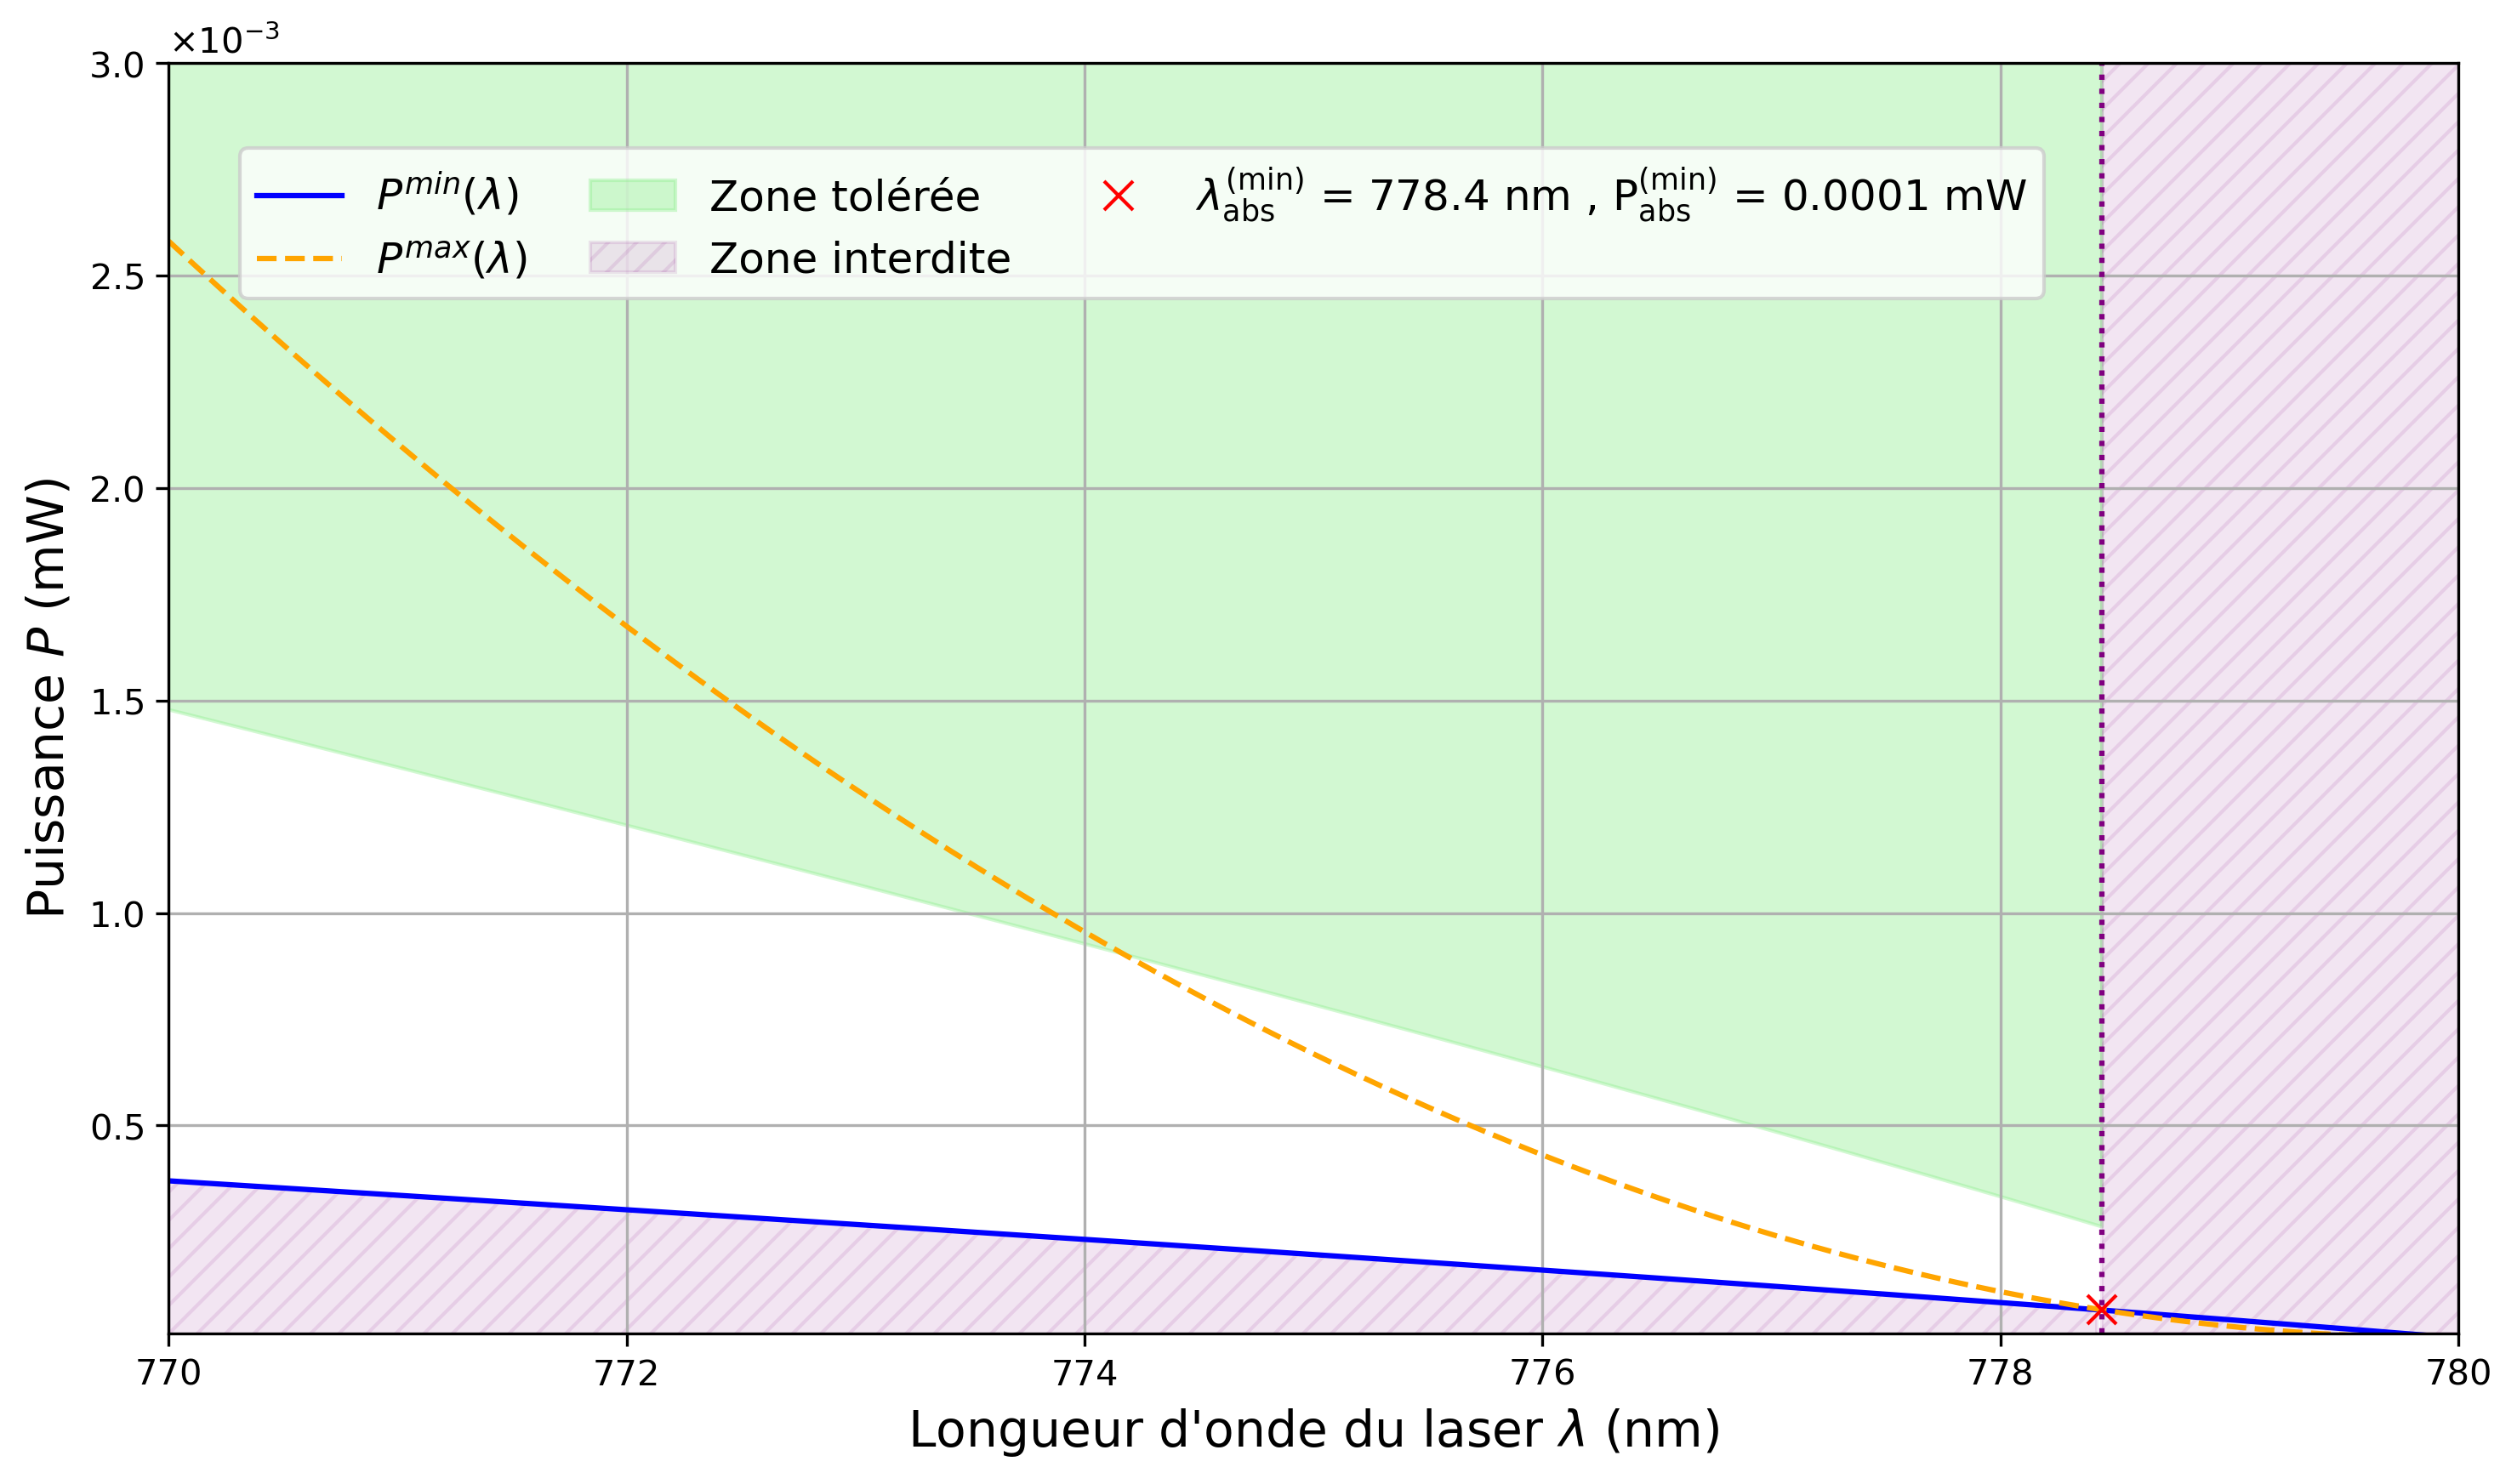
\includegraphics[width=0.7\linewidth]{figures/07_Dipolaire/puissance_vs_lambda_log.png}
    \caption{Puissance requise en fonction de la longueur d'onde pour $w_0 = 1 \, \mu m$ }
\end{figure}

L’intersection de ces courbes définit une {\bf zone de faisabilité expérimentale} dans l’espace $(\lambda, P)$. Le croisement des courbes fournit la longueur d’onde maximale admissible :
\begin{eqnarray*}
	\lambda^{(max)}_{abs} \simeq 778.4~nm , \quad P^{(min)}_{abs} \simeq 0.0001 ~ mW
\end{eqnarray*}

Un premier filtrage des sources laser admissibles impose que la longueur d’onde soit inférieure à $\lambda^{(max)}_{\text{abs}}$ et que la puissance disponible dépasse $P^{(min)}_{\text{abs}}$.

%\subsubsection*{Prise en compte des pertes optiques}
%
%L’ensemble des éléments optiques (fibres, lentilles, miroirs, diviseurs de faisceaux) entraîne une perte totale estimée à environ $40–50\%$, ce qui doit être compensé dès le choix des sources laser. En pratique, la puissance utile disponible au niveau des atomes est :
%\[
%P_{utile} = \eta \cdot P_{laser} \quad \mbox{avec} \, \eta = 0.5 .
%\]

\subsubsection*{Prise en compte des pertes optiques}

L’ensemble des éléments optiques traversés par le faisceau — incluant la sortie de fibre, les lentilles de collimation et de focalisation, les miroirs de redirection, les diaphragmes, ainsi que le diviseur de faisceau — induit des pertes cumulées non négligeables. Une estimation réaliste, fondée sur les caractéristiques typiques des composants et l'expérience de montage, indique que les pertes globales s’élèvent à environ $60$ à $75\%$.

Ces pertes doivent être prises en compte dès le dimensionnement initial du système laser, afin de garantir que la puissance effectivement disponible au niveau des atomes soit suffisante pour atteindre les profondeurs de piège souhaitées. En pratique, on modélise cette efficacité par un facteur global $\eta$, défini comme :
\begin{eqnarray*}
	P_{\text{utile}} = \eta \cdot P_{\text{laser}}, \quad \text{avec} \quad \eta \simeq 0.25.	
\end{eqnarray*}

Ce coefficient sera utilisé dans la suite pour évaluer les puissances minimales requises des sources laser candidates. Une marge de sécurité est également conservée pour pallier les éventuels désalignements ou dégradations optiques en conditions expérimentales réelles.

%%-------------------------
%Un facteur de sécurité supplémentaire est nécessaire si l’on envisage de moduler l’intensité ou d’utiliser des optiques à densité variable.
%\begin{itemize}
%	\item \textbf{DFB (Distributed Feedback)} à $\lambda = 772.5~\text{nm}$, puissance $P = 75~\text{mW}$ : ce type de diode intègre un réseau de Bragg directement dans la cavité pour assurer une émission monomode stable. C’est un choix très répandu pour les applications atomiques.
%	\item \textbf{DBR (Distributed Bragg Reflector)} à $\lambda = 778.0~\text{nm}$, puissance $P = 60~\text{mW}$ : ici, le réseau est séparé de la région active, ce qui offre une certaine souplesse de réglage, bien que la stabilité spectrale puisse être légèrement inférieure à celle des DFB.
%	\item \textbf{DBR} à $\lambda = 770.5~\text{nm}$, puissance $P = 32~\text{mW}$. 
%\end{itemize}
%
%%\begin{center}
%%\textit{[Ajouter une figure montrant les points expérimentaux des lasers DFB et DBR sur le diagramme $(\lambda, P)$]}
%%\end{center}
%
%\paragraph{Pureté spatiale des sources laser}
%
%Les deux sources laser utilisées dans cette expérience sont de type DBR et DFB, toutes deux pigtaillées sur une fibre monomode à maintien de polarisation (PM780-HP). Bien que des modes transverses d’ordre supérieur puissent, en principe, être présents à l’intérieur de la puce laser, la fibre agit comme un filtre spatial efficace. En effet, la fibre PM780-HP ne guide que le mode fondamental LP$_{01}$ (équivalent au mode gaussien TEM$_{00}$) dans la gamme spectrale utilisée ($770{-}780$ nm). Ainsi, la lumière émise en sortie de fibre est spatialement très pure, avec une fraction de puissance dans le mode TEM$_{00}$ supérieure à $99.5\%$.
%
%Cette configuration garantit que les faisceaux utilisés pour le piégeage optique présentent un profil gaussien stable, propre, et bien adapté à une focalisation contrôlée.
%
%
%Les deux lasers sélectionnés se situent dans la zone admissible définie par les conditions $P^{(min)}(\lambda)$ et $P^{(max)}(\lambda)$. Cela valide leur usage pour construire notre boîte optique bleue destinée au piégeage dipolaire de Rubidium-87.
%
%
%-----------------------------

\subsubsection*{Sources laser utilisées et pureté spatiale}

Trois sources laser ont été sélectionnées pour la réalisation de la boîte optique blue-detuned destinée au piégeage dipolaire du Rubidium-87, dont deux répondent aux conditions de puissance admissibles $P^{(min)}(\lambda)$ et $P^{(max)}(\lambda)$.

\begin{itemize}[label = $\bullet$]
    \item \textbf{DFB} à $\lambda = 772.5~\text{nm}$, puissance $P = 75~\text{mW}$.
    \item \textbf{DBR} à $\lambda = 778.0~\text{nm}$, puissance $P = 60~\text{mW}$. 
    \item \textbf{DBR} à $\lambda = 770.5~\text{nm}$, puissance $P = 32~\text{mW}$.
\end{itemize}

\medskip

Le laser DFB (Distributed Feedback) intègre un réseau de Bragg directement dans la région active, ce qui permet un couplage efficace entre la rétroaction optique et le gain, assurant une émission monomode stable tant sur le plan spectral que spatial. Cette architecture confère au DFB une excellente stabilité et une robustesse appréciées en physique atomique.

Le laser DBR (Distributed Bragg Reflector), quant à lui, dispose d’un réseau de Bragg séparé de la région active. Cette configuration offre une plus grande flexibilité dans le réglage de la longueur d’onde, mais entraîne généralement une stabilité spectrale un peu moindre par rapport aux lasers DFB.

\medskip

Ces diodes sont pigtaillées sur des fibres monomodes à maintien de polarisation (type PM780-HP), assurant un profil spatial très pur. En effet, bien que des modes transverses supérieurs puissent être émis par la puce laser, la fibre ne guide que le mode fondamental LP$_{01}$, équivalent au mode gaussien TEM$_{00}$, dans la gamme spectrale $770{-}780~\text{nm}$. Cette configuration agit comme un filtre spatial puissant, garantissant une sortie de faisceau gaussien avec une pureté supérieure à $99.5\%$ en puissance.

\medskip

Cette haute pureté spatiale est cruciale pour obtenir une focalisation optimale et des gradients de champ suffisamment intenses dans la zone de piégeage, tout en minimisant les pertes optiques et les effets parasites liés à la présence de modes non fondamentaux.

Enfin, les troix lasers  se situent dans la zone de tolérence définie par les conditions sur la puissance minimale et maximale en fonction de la longueur d’onde, validant leur adéquation pour la construction de notre boîte optique blue-detuned.

\medskip

Avec un waist de $w_0 = 1~\mu\text{m}$, les puissances minimales requises pour satisfaire les conditions $U_{dip}^{(min)}$ et $\Gamma_{sp}^{(max)}$ sont extrêmement faibles : environ $1.1~\mu\text{W}$ pour la DFB à $772.5~\text{nm}$, $0.3~\mu\text{W}$ pour la DBR à $778.0~\text{nm}$, et $1.4~\mu\text{W}$ pour la DBR à $770.5~\text{nm}$. Ces valeurs sont très largement inférieures aux puissances disponibles pour chacun de ces lasers, même en tenant compte des pertes optiques, ce qui confirme la faisabilité expérimentale du dispositif.

\paragraph{Choix initial du waist.}

Lors de la sélection initiale des lasers, une hypothèse conservative a été faite en supposant un waist focalisé de $w_0 = 300~\text{nm}$ au niveau des atomes. Ce choix était motivé par une estimation de l’échelle typique des variations du potentiel dans la boîte optique, et visait à garantir une intensité suffisante à petite échelle.

\medskip

Avec le recul, cette valeur s’est avérée trop pessimiste. Le système optique finalement mis en place permet des waists plus larges (de l’ordre du micron), mieux adaptés à la géométrie expérimentale et aux contraintes de focalisation. Cette hypothèse initialement sous-estimée a toutefois eu pour effet bénéfique de conduire à une surévaluation des puissances requises, fournissant une marge de sécurité bienvenue dans le dimensionnement des sources laser.

\medskip

Avec un waist de $w_0 = 300~\mu\text{m}$, les puissances minimales requises augmentent considérablement en raison de la baisse d’intensité au centre du faisceau. On obtient alors des puissances nécessaires de l’ordre de $102~\text{mW}$ pour la DFB à $772.5~\text{nm}$, $30~\text{mW}$ pour la DBR à $778.0~\text{nm}$, et $127~\text{mW}$ pour la DBR à $770.5~\text{nm}$. Seul le laser à $778.0~\text{nm}$ satisfait cette condition sans amplification supplémentaire. En revanche, les deux autres lasers se trouvent sous-dimensionnés dans ce scénario, ce qui justifie le recours à un amplificateur optique dans le cas du laser à $770.5~\text{nm}$.

\begin{figure}[H]
    \centering
    \includegraphics[width=0.7\linewidth]{figures/07_Dipolaire/puissance_vs_lambda_log_300.png}
    \caption{Puissance requise en fonction de la longueur d'onde pour $w_0 = 300 \, \mu m$ }
\end{figure}

\medskip

Ce constat a notamment motivé l’ajout d’un amplificateur optique (TA — Tapered Amplifier) en sortie du laser à $770.5~\text{nm}$, afin de compenser la puissance disponible limitée et garantir des conditions de piégeage satisfaisantes malgré les pertes optiques du système.

\begin{center}
\textit{[Photos laser à $770.5~\text{nm}$ ]}
\end{center}


\subsection{Amplification par Tapered Amplifier (TA)}

% INSERTION FIGURE  
\begin{figure}[!htb]
	\centering
	\begin{tikzpicture}
    	\node[rectangle, draw = none] (A) at (0,0) {
       		
\includegraphics[width=0.8\textwidth , page = 7]{figures/07_Dipolaire/Figures}
    	};
\end{tikzpicture}
\caption{Schéma global de l’amplification}
\label{fig:TA_setup}

\end{figure}

\subsubsection*{Principe et motivation}

Afin de compenser le déficit de puissance du laser DBR à $770.5~\text{nm}$ — notamment dans le scénario initialement envisagé avec un waist focalisé important — un amplificateur optique de type \textit{Tapered Amplifier} (TA) a été ajouté en aval de la source laser.

Un TA est un semi-conducteur optique amplificateur non résonant, composé d'une région d'entrée étroite (guidée) et d'une région de sortie évasée (tapered), permettant d'amplifier efficacement un faisceau monomode tout en conservant un profil spatial de bonne qualité. Contrairement aux lasers, le TA n'oscille pas par lui-même : il agit uniquement sur un signal incident (seed). Il peut amplifier des puissances faibles (quelques mW) en entrée jusqu’à plusieurs centaines de mW, voire au-delà, en sortie.

Ce dispositif est particulièrement adapté aux expériences de piégeage optique, où une puissance laser relativement élevée est nécessaire tout en maintenant une bonne qualité spatiale.

\subsubsection*{Contraintes et précautions}

L'utilisation d’un TA s’accompagne de plusieurs contraintes expérimentales importantes :

\begin{itemize}[label=$\bullet$]
    \item \textbf{Sensibilité aux rétro-réflexions :} la puce du TA ne supporte pas les retours optiques parasites, qui peuvent entraîner des instabilités, des dégradations de performance, voire endommager le composant. Un \textbf{isolateur optique} est donc placé en sortie pour bloquer tout retour de lumière vers le TA.
    
    \item \textbf{Sensibilité à l’alignement :} une injection efficace du faisceau dans la zone guidée d’entrée du TA requiert un alignement très précis. Celui-ci est réalisé à l’aide de deux miroirs montés sur des supports à réglage fin, offrant 4 degrés de liberté (translations X–Y, inclinaisons $\theta_x$, $\theta_y$).
    
    \item \textbf{Émission multi-modes en sortie :} malgré une injection monomode, la sortie du TA présente parfois plusieurs lobes d’intensité dus à la géométrie évasée. Un diaphragme ou une \textbf{pinhole} de $50~\mu$m (à ajuster selon le profil observé) est donc utilisé pour filtrer spatialement le mode fondamental TEM$_{00}$.
\end{itemize}

\subsubsection*{Mise en œuvre expérimentale}

Le schéma global de l’amplification est présenté sur la figure~\ref{fig:TA_setup} .

\begin{itemize}[label=$\triangleright$]
    \item \textbf{Laser seed :} le laser DBR à $770.5~\text{nm}$ est stabilisé en température et en courant à l’aide du contrôleur Thorlabs ITC-510, et injecté dans le TA à l’aide d’une optique de couplage sur table optique.
    
    \item \textbf{Boîtier de protection et régulation thermique :} le TA est installé dans un boîtier métallique maison, conçu pour assurer à la fois une protection mécanique et une stabilité thermique. Ce boîtier intègre un module Peltier et une thermistance pour la régulation active de la température, pilotés par un contrôleur thermique (Arrow OEM). L’ensemble est alimenté par une alimentation dédiée (Delta Electronics), garantissant un fonctionnement stable du système de refroidissement. Cette stabilisation thermique est cruciale pour limiter les dérives du TA et préserver la qualité spatiale du faisceau amplifié.

    \item \textbf{Filtrage spatial :} un diaphragme (pinhole) placé dans le plan de Fourier d’un système en configuration télescopique, positionné en sortie de l’amplificateur TA, permet de sélectionner efficacement le mode spatial fondamental.

    \item \textbf{Isolateur optique :} un isolateur optique est placé immédiatement après le TA pour éviter tout retour de lumière vers la puce.

    \item \textbf{Modulation de puissance :} un modulateur acousto-optique (AOM) est inséré juste avant la fibre optique, permettant de couper la lumière à la demande (switch rapide) ou de moduler dynamiquement l’intensité laser. Cela permet un contrôle fin de l’illumination au niveau des atomes.
    
    \item \textbf{Mesure de puissance :} une photodiode ou un power meter placé après l’AOM permet de calibrer précisément la puissance en fonction du courant injecté dans le TA, et de corriger les effets d’instabilité si besoin.
\end{itemize}

\subsubsection*{Caractérisation et performance}

La diode laser et le Tapered Amplifier (TA) sont asservis à une température stable de $25^\circ$C. Une courbe de puissance de sortie du TA en fonction du courant injecté a été mesurée (voir figure~\ref{fig:Puissance_TA}), avec la diode laser fonctionnant à $25^\circ$C et délivrant une puissance maximale d’environ $31.2\,\text{mW}$, tandis que le TA est testé jusqu’à un courant d’injection de $2.5\,\text{A}$.

\begin{figure}[H]
    \centering
    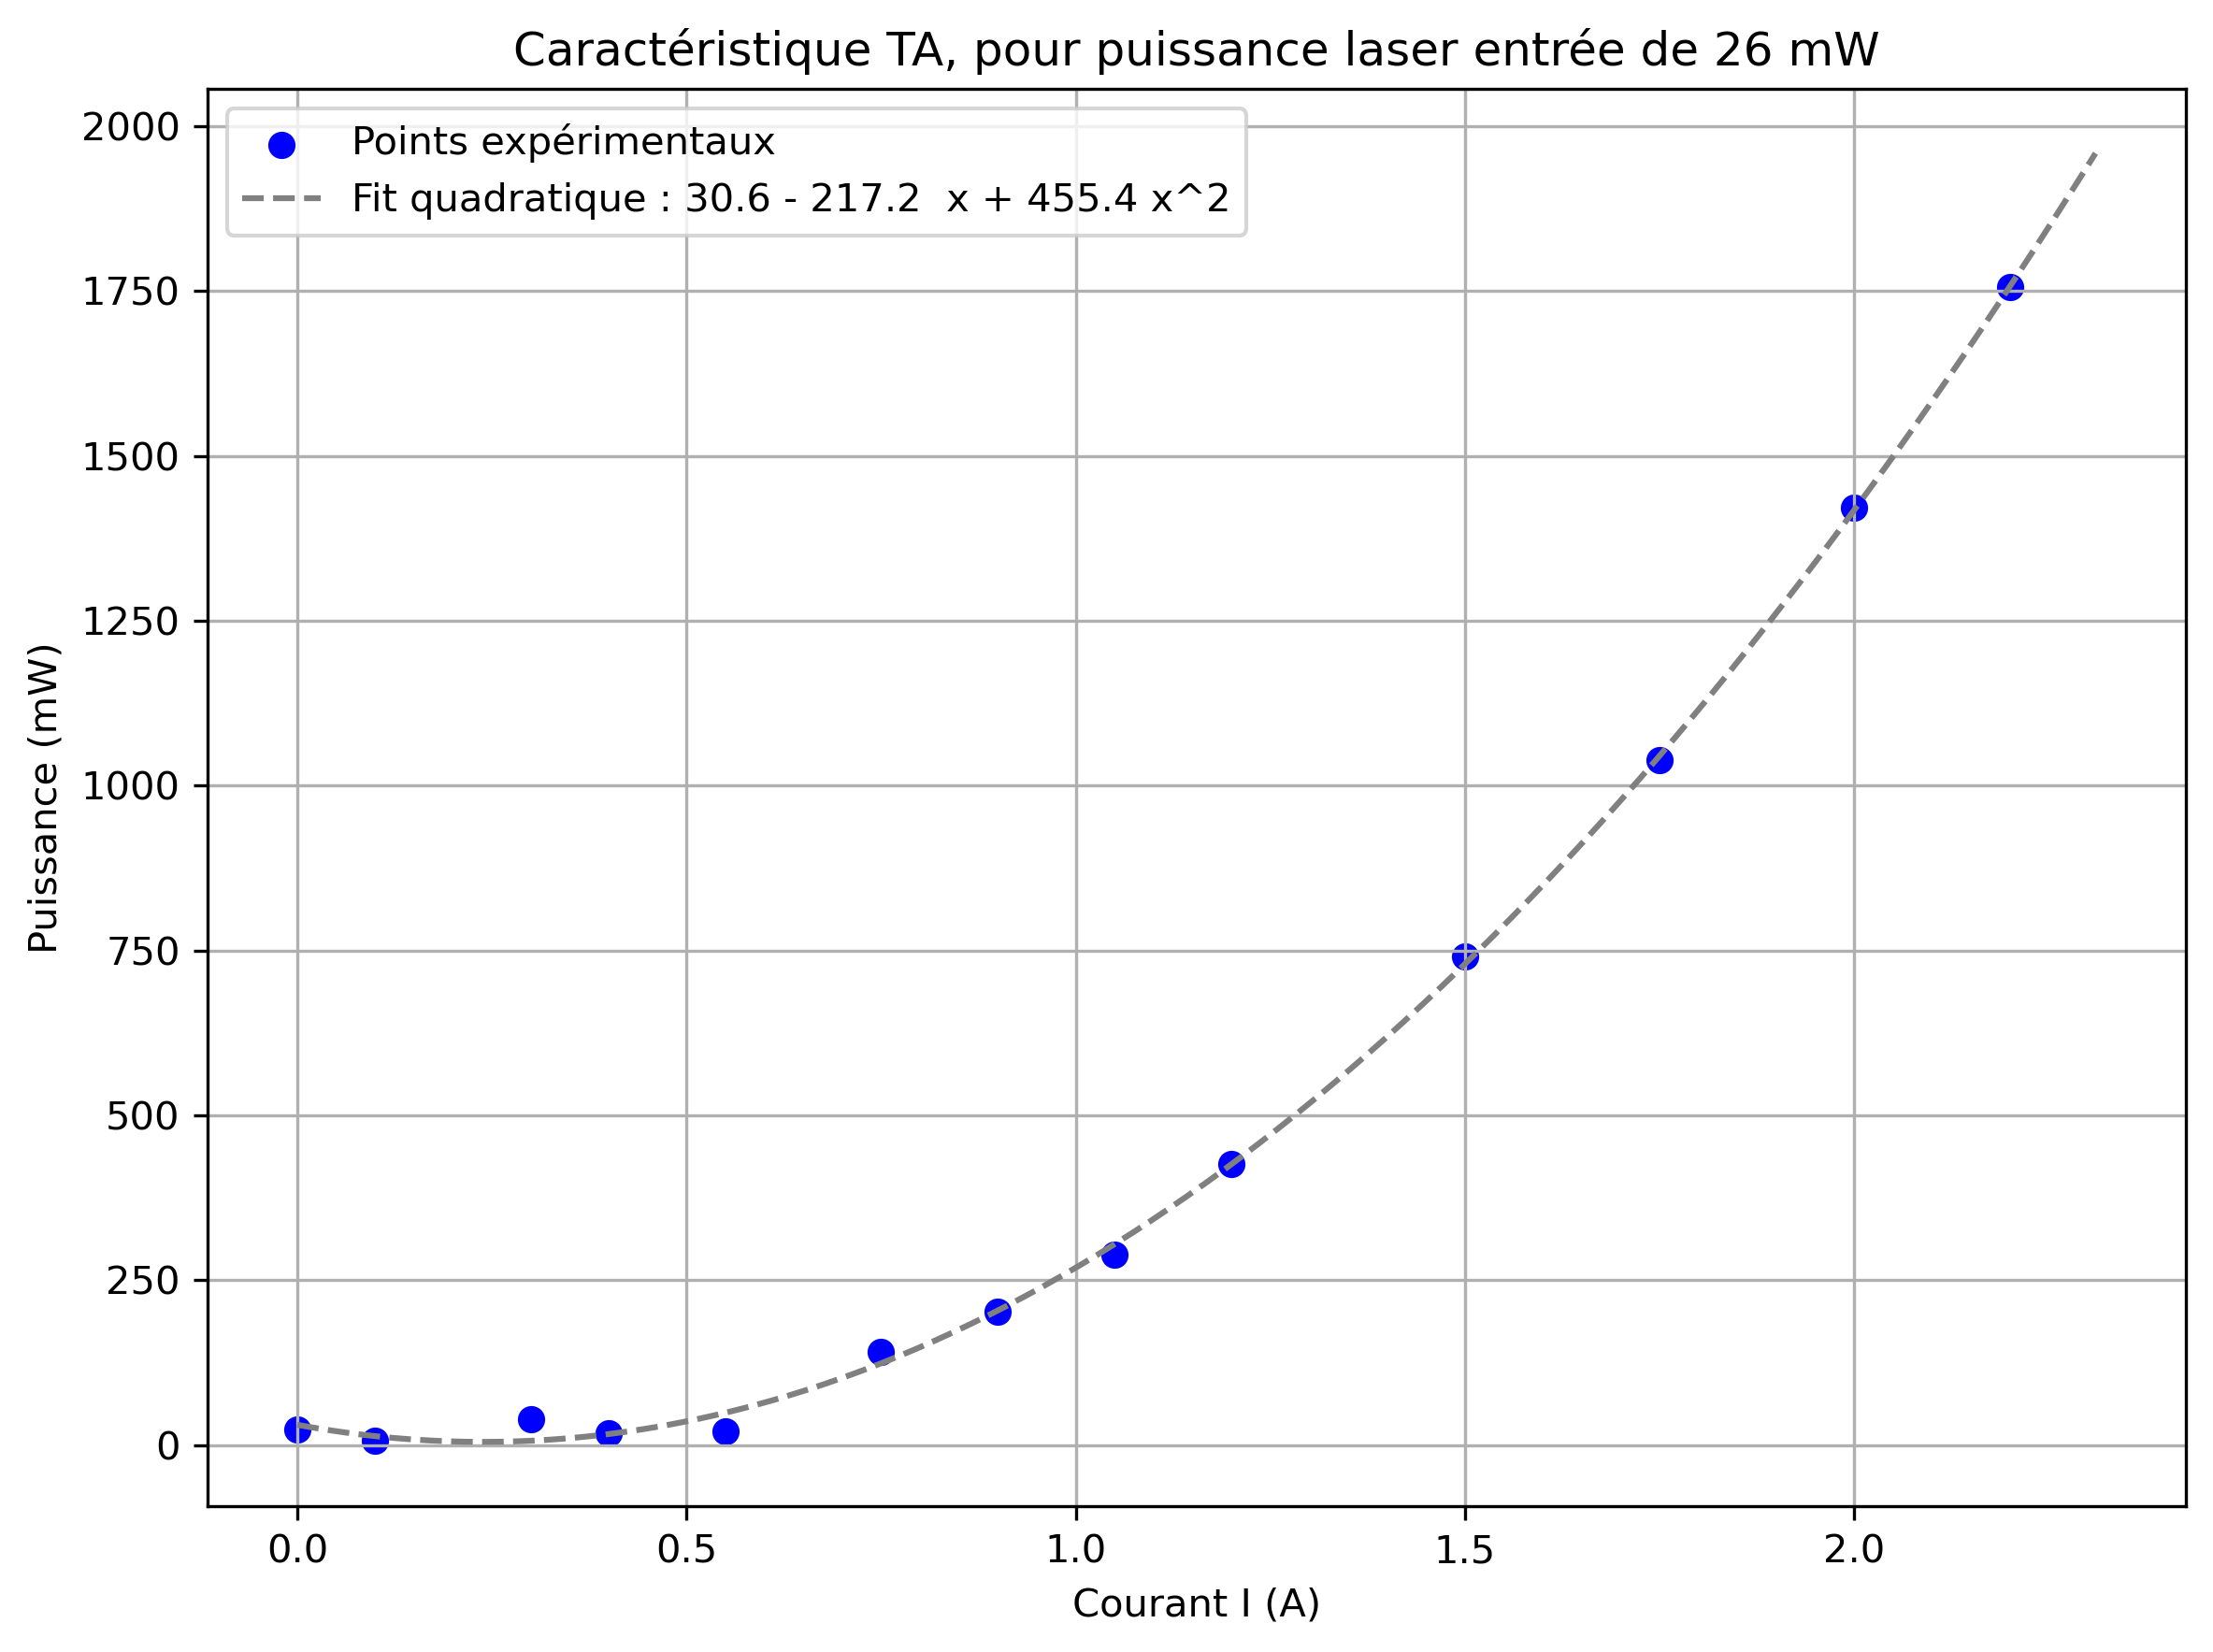
\includegraphics[width=0.7\linewidth]{figures/07_Dipolaire/Puissance_TA.png}
    \caption{Puissance de sortie du Tapered Amplifier (TA) en fonction du courant d’injection, pour une puissance d’entrée provenant de la diode laser fixée à 25 mW.}
    \label{fig:Puissance_TA}
\end{figure}

Afin d’éviter une dégradation prématurée des composants, il a été choisi de ne pas les faire fonctionner à leurs limites maximales. La diode laser est ainsi réglée pour fournir une puissance d’environ $25\,\text{mW}$ (courant $I_{\text{diode}} = 150.6\,\text{mA}$) et le TA est exploité avec un courant d’environ $1.5\,\text{A}$. Cette configuration assure un bon compromis entre puissance de sortie et longévité des dispositifs, tout en garantissant une amplification stable et un profil spatial préservé.

Pour un courant d’injection de $1.5\,\text{A}$ dans le TA, la puissance mesurée en sortie, après passage dans le modulateur acousto-optique (AOM), atteint environ $62\,\text{mW}$. 

L’AOM génère plusieurs ordres de diffraction : le mode zéro (non diffracté), les modes $\pm 1$, etc. Afin d’optimiser le transfert d’énergie dans un mode diffracté souhaité (par exemple le premier ordre $\pm 1$), le cristal AOM a été ajusté finement en rotation. Ce réglage permet de maximiser la puissance dans ce mode non nul.

Le faisceau correspondant à ce mode diffracté, qui concentre la majorité de la puissance utile, est ensuite injecté dans une fibre monomode à maintien de polarisation. 

Ainsi, l’AOM est configuré de manière à transférer efficacement la puissance vers le mode diffracté utile, avec une puissance d’environ $62\,\text{mW}$ disponible à l'entée de la fibre, garantissant une qualité spatiale et une polarisation stables pour l’expérience.


Le système ainsi mis en place permet d’obtenir, de manière stable, une puissance suffisante en sortie pour alimenter la fibre de piégeage, même en tenant compte des pertes optiques du système.



%Le projet est de fais une boite en utilisant un potentielle dipolaire électique induite par un laser dans la longeur d'onde et decaler dans le blue ($\Delta > 0 $) par raport au transition D1 et D2 des atomes de Rubidium97. 
%On partie d'un systeme d'atome froid , unidimentionelle. On fait dest faiseaux dipolaires à diferrent postions. Les atomes seron confiné dans la zone entre les faiseaux. 
%
%\vspace{1em}
%% INSERTION FIGURE
%\begin{center}
%\textit{[Insérer ici schéma des deux faiseaux avec les atomes au milieux]}
%\end{center}
%
%Maintent , il faux caracteriser ces faisceaux. Dans un premier tempst on a avus Il y a 2 parametre a prend en compte , les potentiel pic aux niveau des atomes $U_{dip}(0)$ , qui impluence la profondeur du puit , les Taux d'emition spontané pic $\Gamma_{sp}(0)$ qui influence .... .
%On veux que $U_{dip}(0)$ soit siperieur a une maleur minimur , que pour les calcule futur on noterar $U_{dip}^{(min)}(0)$ , cette valeur serais de $1 k_B \times \mu K $ (pour .... peut etre une raison dans la literature ) , et puis on impose que pour $x^\ast$ tel que $U_{dip}(x^\ast)= U_{dip}(0)/2$ , $\Gamma_{dip}(x^\ast)$ imferieur à une valeur maximume de $2\pi \times 1 s^{-1}$. En remarquant les potentielle $U_{dip}(\vec{r})$  et le taux de difusions $\Gamma_{sp}(\vec{r})$ sont proportionnelle à l'intentité $I(\vec{r})$ , on constante que cette dernier condition est equivalente à $\Gamma_{sp}(0) \leq \Gamma_{sp}^{(max)}(0) = 2\pi \times 2 ~s^{-1}$. 
%
%\paragraph{Ratio figure de mérite : potentiel / diffusion}
%Il est utile de comparer le potentiel conservatif $U_{dip}$ au taux de diffusion $\Gamma_{sc}$ pour quantifier l’efficacité du piégeage :
%\begin{eqnarray*}
%	\frac{U_{dip}(\vec{r})}{\hbar \Gamma_{sc}(\vec{r})} = \frac{1}{\Gamma} \frac{ \left( \frac{ 1}{ 3 \Delta_1} + \frac{2 }{ 3 \Delta_2}  \right )}{\left( \frac{ 1}{ 3 \Delta_1^2} + \frac{2 }{ 3 \Delta_2^2}  \right )} \geq \frac{U_{dip}^{(min)}(0)}{\hbar \Gamma_{sc}^{(max)}(0)}.
%\end{eqnarray*}
%Ce rapport est homogène à une {\bf fréquence}, et correspond à l’inverse d’un {\bf temps caractéristique} entre deux événements de diffusion. Plus il est grand, plus le piégeage est efficace avec peu d’échauffement. Il permet également d’estimer :
%\begin{itemize}[label=$\bullet$]
%	\item La {\bf longueur d’onde optimale} (balancement entre profondeur de piège et faible taux de diffusion),
%	\item La {\bf puissance minimale nécessaire}  à une barrière donnée,
%	\item La {\bf faisabilité}  d’un piège blue-detuned (ou red-detuned).
%\end{itemize}
%
%Un calcule numérique , nous dit que avec cette condition on doit chercher des laser avec des longueur d'onde inferieux-r a la longeur d'onde max $\lambda^{(max)} = 778,4 ~ nm$.
%
%(	\item La {\bf puissance minimale nécessaire}  à une barrière donnée,
%	\item La {\bf faisabilité}  d’un piège blue-detuned (ou red-detuned).
%comment ????? 
%) 
%
%c'est une premier information mais les faiseaux sera gaussien avec un waist $w_0$ des quelque centaine de nm (car ....) . 
%Avec $I(0) = \frac{2P}{\pi w_0^2}$ , avec $P$ la puissance du laser. On deux condition qui bornent la puissance du laser pour un longeur du laser $\lambda$ d'on donné : 
%
%\begin{eqnarray*}
%	 \underbrace{U_{dip}^{(min)}(0) \frac{\pi w_0^2}{2} \frac{8 I_{sat}}{\Gamma^2}\left/\left( \frac{ 1}{ 3 \Delta_1} + \frac{2 }{ 3 \Delta_2}  \right ) \right.}_{P^{(min)}(\lambda)}  \leq P(\lambda) \leq \underbrace{ \Gamma_{sc}^{(max)}(0) \frac{\pi w_0^2}{2} \frac{8 I_{sat}}{\Gamma^3}\left/\left( \frac{ 1}{ 3 \Delta_1^2} + \frac{2 }{ 3 \Delta_2^2}  \right )\right.}_{ P^{(max)}(\lambda)} 
%\end{eqnarray*}
%
%\vspace{1em}
%% INSERTION FIGURE
%\begin{center}
%\textit{[Insérer ici schéma des courbe P ]}
%\end{center}
%
%Sur cette figure on a representer cest deux courbe , P^{(min)} , P^{(max)} , une croix rouge represente là ous les deux courbe se croise , la cordonnée $(\lambda^{(max)} , P^{(min)}_{abs})$. Un filtrege grossier pour le chois de nos laser est un laser avec une longeur d'onde inferieur a $\lambda^{(max)} = ... $ et une puicane superieur à $P^{(min)}_{abs} = ...$.
%
%LA puiscent du laser au niveau des atomes doit etre pour une longeur d'onde donnet etre danst les zone etre les deux courbe.
%J'estimes que les perter du au optique est de ???\% (fibre optique , miroire , lentille et deboublement du du faisseaux  ) . Et biens sur si la puissance est trop brande on peut ajouter des densité opitique donc , avec cette marge de ???\% je choix des lazer doit etre dans la zone bleu sur la figure .
%J'ai selectionner 2 laser avec les cacteristique suivante :
%
%\begin{itemize}
%	\item DFB de longueur d'onde $772.5 ~nm$ et de Puissance $75.0~ mW$ ( les point rouge sur la figure  
%	\item DBR de longueur d'onde $778.0 ~nm$ et de Puissance $60.0~ mW$ ( les point blue sur la figure 	
%\end{itemize}














%\subsubsection{Quelle longueur d'onde ?}







\chapter*{Conclusion}
\addcontentsline{toc}{chapter}{Conclusion}

Conclusion de la thèse.


\appendix
\chapter{Annexes}

Informations complémentaires.



\bibliographystyle{unsrt}
\bibliography{thesis}

\end{document}


\section{Rôle des charges conservées extensives et quasi-locales}
%Dans les systèmes intégrables, l’état stationnaire atteint après une évolution hors d’équilibre n’est généralement pas décrit par un état de Gibbs classique, mais par un ensemble généralisé de Gibbs (GGE). Celui-ci est construit à partir de toutes les charges conservées du système

\paragraph{Écriture des observables thermodynamiques comme sommes sur les rapidités.}

%Dans le cas thermique, les valeurs moyennes des observables classiques telles que le nombre de particules et l'énergie peuvent s'exprimer comme des sommes de puissances des rapidités :
Dans un système à $N$ particules caractérisé par des rapidités $\{ \theta_a \}_{a = 1}^N$, les charges conservées classiques — telles que le nombre de particules, l’impulsion ou l’énergie — s’écrivent comme des sommes de puissances des rapidités :
\(
	\langle \operator{Q} \rangle_{\{ \theta_a\} } \propto \sum_{a = 1}^N \theta_a^0 , \,  \langle \operator{P} \rangle_{\{ \theta_a\} } \propto \sum_{a = 1}^N \theta_a^1  ,\,  \mbox{et} \langle \operator{K} \rangle_{\{ \theta_a\} } \propto \sum_{a = 1}^N \theta_a^2 .	
\)
(cf. équations \eqref{chap.2.gge.1})
Dans ce paragraphe précédent, nous avons sous-entendu — sans l’expliciter — qu’il est montré que l’ensemble des charges locales conservées forme une famille donnée par :
\begin{eqnarray}
	\operator{Q}_i^{(\mathcal{S})} \ket{\{\theta_a\} } & \propto & \sum_a \theta_a^i \ket{\{\theta_a\} }.
\end{eqnarray}
Ces charges agissent donc de manière diagonale sur les états de Bethe, avec des valeurs propres correspondant aux moments des rapidités.
%%%%%%%%%%%%%%%%%%%%%%%%%%%%%%%%%%%%%%%%%%%%%%%%%%
\paragraph{Charges locales conservées .\label{sec:charges-gen}}

%Les états propres du Hamiltonien de Lieb–Liniger~\eqref{eq:LL} sont les états de Bethe
%\(
%  \ket{\boldsymbol{\theta}}
%  =\ket{\theta_1,\dots,\theta_N}\!,
%\)
%déterminés par leurs rapidités \(\boldsymbol{\theta}\).

À toute fonction régulière
\(
  f:\mathbb R\!\to\!\mathbb R
\)
on associe un opérateur-charge loclal :
\begin{eqnarray}\label{chap.2.charge.f.1}
	\operator{\mathcal{Q}}^{(\mathcal{S})}[f] & = &  L \int_0^L d\theta \, f(\theta) \operator{\rho}^{(\mathcal{S})}(\theta).	
\end{eqnarray}
où $\operator{\rho}(\theta)$ agit sur une état de Bethe comme 
\begin{eqnarray}\label{chap.2.rho.1}
	 \operator{\rho}(\theta) \ket{ \{ \theta_a \} } &=& \frac{1}{L} \sum \delta ( \theta - \theta_a ) \ket{ \{ \theta_a \} }.	
\end{eqnarray}
De sorte que $\operator{\mathcal{Q}}^{(\mathcal{S})}[f]$ agit sur une état de Bethe comme
\begin{eqnarray}\label{chap.2.charge.1}
	\operator{\mathcal{Q}}^{(\mathcal{S})}[f]\,\ket{\{\theta_a\} } =  \sum_{a=1}^{N}f(\theta_a)\,\ket{\{\theta_a\} } \quad \mbox{de sorte que} \quad \braket{\operator{\mathcal{Q}}^{(\mathcal{S})}[f]}_{\{\theta_a\}} = \sum_{a=1}^N f(\theta_a)
\end{eqnarray}
Les choix particuliers
\(
  f_0(\theta)=1
\)
,
\(
  f_1(\theta)=\theta
\)
et
\(
  f_2(\theta)=\theta^{2}/2
\)
redonnent respectivement l'opérateur nombre \(\operator{Q}=\operator{Q}_0^{(\mathcal{S})} = \operator{\mathcal{Q}}^{(\mathcal{S})}[1]\) , impulsion \(\operator{P}=\operator{Q}_1^{(\mathcal{S})} = \operator{\mathcal{Q}}^{(\mathcal{S})}[\theta]\) et énergie cinétique
\(\operator{K}=\operator{Q}_2^{(\mathcal{S})} = \operator{\mathcal{Q}}^{(\mathcal{S})}[\theta^2/2]\). Et dans le cadre des (GGE), pour tous les ordres $i$ on note :
\begin{eqnarray}\label{chap.2.charge.ordre.i.1}
	\operator{Q}^{(\mathcal{S})}_i = \operator{\mathcal{Q}}^{(\mathcal{S})}[f_i]	, \quad \mbox{de sorte que} \quad \braket{\operator{Q}^{(\mathcal{S})}_i}_{\{\theta_a\}} = \sum_{a=1}^N f_i(\theta_a)  
\end{eqnarray}
avec les densités spectrales $f_i(\theta) \propto \theta^i$ . 

Ces charges sont extensives : leur densité locale $\operator{q}^{(\mathcal{S})}_{[f]}$ permet d’écrire
\(
  \operator{\mathcal{Q}}^{(\mathcal{S})}[f]=\int_0^{L}\!dx\;\operator{q}^{(\mathcal{S})}_{[f]}(x).
\)

\paragraph{Charges conservées généralisée.\label{sec:charges-gen}}
Les fonction $f_i$ étant fixées, on note la fonction régulière
\(
  w:\mathbb R\!\to\!\mathbb R
\)
–– dorénavant appelée \emph{poids spectral}, ou \emph{potentiel spectral} ––
\begin{eqnarray}
	w = \sum_i \beta_i f_i \label{chap.2.w.1},	
\end{eqnarray}
on associe un opérateur-charge généralisé $\operator{\mathcal{Q}}^{(\mathcal{S})}[w]$ :
\begin{eqnarray}\label{chap.2.charge.gen.1}
	\operator{\mathcal{Q}}^{(\mathcal{S})}[w]\,\ket{\{\theta_a\} } =  \sum_{a=1}^{N}w(\theta_a)\,\ket{\{\theta_a\} } \quad \mbox{de sorte que} \quad \braket{\operator{\mathcal{Q}}^{(\mathcal{S})}[w]}_{\{\theta_a\}} = \sum_{i} \beta_i  \braket{\operator{Q}^{(\mathcal{S})}_i}_{\{\theta_a\}}
\end{eqnarray}

%%%%%%%%%%%%%%%%%%%%%%%%%%%%%%%%%%%%%%%%%
\paragraph{Expression de la matrice densité généralisée.}
La matrice densité  s’écrit sous la forme :
L’ensemble général défini par $\operator{\rho}^{(\mathcal{S})}[w]$ 
\begin{eqnarray}\label{chap.2.densite.1}
	\operator{\rho}^{(\mathcal{S})}[w]  =  \frac{e^{-\operator{\mathcal{Q}}^{(\mathcal{S})}[w]}}{Z^{(\mathcal{S})}[w]}, \, \mbox{avec} \quad e^{-\operator{\mathcal{Q}}^{(\mathcal{S})}[w]}  = 	\sum_{\{\theta_a \}} e^{- \sum_{a = 1}^N w(\theta_a) } \vert \{ \theta_a\} \rangle \langle  \{ \theta_a\}  \vert, 
\end{eqnarray}	
	%pour une certaine fonction $w$ relié à la charge% $\operator{\mathcal{Q}} [w]  = \sum_{\{\theta_a \}} \left ( \sum_{a = 1}^N w ( \theta_a )  \right ) \vert \{ \theta_a \} \rangle \langle \{ \theta_a \} \vert $.
%où l'opérateur de charge associé à $w$ s’écrit :
%\begin{eqnarray}
%	\operator{\mathcal{Q}} [w]   & = &  \sum_{\{\theta_a \}} \left ( \sum_{a = 1}^N w ( \theta_a )  \right ) \vert \{ \theta_a \} \rangle \langle \{ \theta_a \} \vert,	
%\end{eqnarray}
et la fonction de partition \eqref{chap.TBA.op.Z.S} s'écrit $Z^{(\mathcal{S})}[w]\doteq \bm{\mathrm{Tr}}\left [ e^{-\operator{\mathcal{Q}}^{(\mathcal{S})}[w]}\right ] $ vaux :
\begin{eqnarray}
	Z^{(\mathcal{S})}[w]   =  \sum_{\{\theta_a \}} e^{-\sum_{a = 1}^N w(\theta_a)},\label{chap.TBA.op.Z.S.1}	
\end{eqnarray}
devient un Generalized Gibbs Ensemble (GGE), $\operator{\rho}^{(\mathcal{S})}_{\mathrm{GGE}}$ (de l'équation \eqref{chap.TBA.op.rho.S})	 dès lors que $w(\theta) = \sum_i \beta_i f_i(\theta)$ (de l'équation \eqref{chap.2.w.1}) où $f_i$ sont les densités spectrales associées aux charges locales conservées (de l'équation \eqref{chap.2.charge.ordre.i.1}).


%%%%%%%%%%%%%%%%%%%%%%%%%%%%%%%%%%
\paragraph{Probabilité associée à une configuration de rapidités.}
	%Et on peut réecrire la probabilité de la configuration $\{\theta_a\}$ :% $ P_{\{ \theta_a \}} = \langle \{ \theta_a \}\vert \operator{\rho}_{GGE}[w] \vert  \{ \theta_a \} \rangle = e^{-\sum_{a = 1}^N w(\theta_a)} / Z $ avec $Z = \sum_{\{\theta_a \}} e^{-\sum_{a = 1}^N w(\theta_a)}$.\\
	%La probabilité d’occuper un état à $N$ particules caractérisé par les rapidités ${\theta_a}$ est alors :
Dans ce formalisme, la probabilité d’occuper l’état $\ket{\{\theta \}}$ \eqref{chap.TBA.P.1} est donc
\begin{eqnarray}
	\mathbb{P}^{(\mathcal{S})}_{\{ \theta_a \}} & = &  Z^{(\mathcal{S})}[w]^{-1}e^{-\sum_{a = 1}^N w(\theta_a)}\label{chap.TBA.P.w.2}. 		
\end{eqnarray}
%Cela montre que le poids statistique d’une configuration factorise naturellement sur les pseudo-moments, avec un poids spectrale / energie génralisé $w(\theta)$ attribué à chaque particule.
On voit ainsi que le poids statistique factorise naturellement sur les
pseudo‑moments, chaque particule étant pondérée par $w(\theta_a)$.

%avec 
%\begin{eqnarray}
%	Z  & = & \sum_{\{\theta_a \}} e^{-\sum_{a = 1}^N w(\theta_a)}.		
%\end{eqnarray}


%%%%%%%%%%%%%%%%%%%%%%%%
\paragraph{Moyennes d'observables dans le GGE.}
%La valeur moyenne d’un observable locale $\operator{\mathcal{O}}$ dans l’ensemble généralisé s’écrit :
Pour tout opérateur local $\operator{\mathcal{O}}$ diagonal dans la base de Bethe,
la moyenne généralisée vaut
\begin{eqnarray}\label{chap.2.moyenne.1}
	\langle \operator{\mathcal{O}}\rangle_{\operator{\rho}^{(\mathcal{S})}[w]} & = & \displaystyle   \frac{\sum_{\{\theta_a \}} \braket{ \operator{\mathcal{O}}}_{\{ \theta_a\}} e^{- \sum_{a = 1}^N w(\theta_a) }  }{\sum_{\{\theta_a  \}} e^{- \sum_{a = 1}^N  w(\theta_a) } }
\end{eqnarray}
%Cette expression formelle montre que la connaissance de $w(\theta)$ suffit à déterminer les propriétés statistiques de toutes les observables diagonales dans cette base, incluant les charges conservées elles-mêmes.
Ainsi, la connaissance de la fonction $w(\theta)$ suffit à déterminer
les propriétés statistiques de toute observable diagonale,
y compris les charges conservées elles‑mêmes.	
	% Nous aimerions calculer les valeurs d'attente par rapport à cette matrice de densité, par exemple
	%La moyenne GGE d'un observable s'écrit ,
	%\begin{aff}
	%\begin{eqnarray}
	%	\langle \operator{\mathcal{O}} \rangle_{GGE} & \doteq & \displaystyle  \text{Tr} (\operator{\mathcal{O}}\operator{\rho}[w]) = \frac{\text{Tr} (\operator{\mathcal{O}}e^{-\operator{\mathcal{Q}}[w]})}{\text{Tr} (e^{-\operator{\mathcal{Q}}[w]})}	 = \frac{\sum_{\{\theta_a \}} \langle  \{ \theta_a\}  \vert   \operator{\mathcal{O}} \vert \{ \theta_a\} \rangle e^{- \sum_{a = 1}^N w(\theta_a) }  }{\sum_{\{\theta_a  \}} e^{- \sum_{a = 1}^N  f(\theta_a) } }
		%& =  & \frac{ \sum_{\pi} \sum_{\vert \{\theta_a \}\rangle \vert \Pi } \langle  \{ \theta_a\}  \vert   \operator{\mathcal{O}} \vert \{ \theta_a\} \rangle e^{- \sum_{a = 1}^N f(\theta_a) }  }{\sum_{\pi} \sum_{\vert \{\theta_a \}\rangle \vert \Pi }  e^{- \sum_{a = 1}^N  f(\theta_a) } }
	%\end{eqnarray}
	%pour une certaine observable $\operator{\mathcal{O}}$.\\
	%\end{aff}
	

\paragraph{Conclusion de la section : vers la thermodynamique de Bethe.}

Nous avons vu que, dans un système intégrable, la description correcte de l’équilibre stationnaire requiert l’introduction d’une \emph{famille infinie de charges conservées}, comprenant à la fois des charges strictement locales et des charges quasi‑locales.
Toutes ces charges se réunissent dans l’opérateur fonctionnel
\(
\operator{\mathcal{Q}}^{(\mathcal{S})}[w]
\)
, défini par un \emph{poids spectral}  $w(\theta)$ (cf. équations~\eqref{chap.2.charge.1}).
Cette construction conduit naturellement à la matrice densité généralisée
\(
\operator{\rho}^{(\mathcal{S})}_{\mathrm{GGE}}[w]  \propto  e^{-\operator{\mathcal{Q}}^{(\mathcal{S})}[w]}
\) 
(cf. équations~\eqref{chap.2.densite.1}), et à la moyenne d’un opérateur local $\operator{\mathcal{O}}$ donnée par
\(
\langle \operator{\mathcal{O}}\rangle_{GGE}  \doteq  \displaystyle  \text{Tr} (\operator{\mathcal{O}}\operator{\rho}^{(\mathcal{S})}_{\mathrm{GGE}}[w])
\)
(cf. équations~\eqref{chap.2.moyenne.1}).
La connaissance de $w(\theta)$ suffit donc pour prédire les valeurs moyennes de toutes les observables diagonales, y compris celles des charges elles‑mêmes ; c’est le cœur du {\bf Ensemble de Gibbs Généralisé (GGE pour Generalized Gibbs Ensemble)} .

\medskip
Cette base est désormais posée : dans la section suivante, nous passerons au \emph{thermodynamique de Bethe}.
Nous verrons comment, dans la limite thermodynamique, les sommes sur les configurations de rapidités se transforment en intégrales sur des densités continues, comment apparaît l’entropie de Yang–Yang, et comment les moyennes de l’ensemble généralisé se réexpriment à l’aide de ces densités macroscopiques.
C’est ce formalisme qui permettra d’analyser finement la relaxation post‑quench et de relier microscopie intégrable et hydrodynamique généralisée.



%% !TEX encoding = IsoLatin

%\documentclass[11pt,a4paper]{report}
%\documentclass[11pt,a4paper]{book}
\documentclass[10pt, titlepage]{book} % Taille de base des caractères (12pt recommandée pour lecture)


% -------------------------------------
% Encodage et langue
% -------------------------------------
\usepackage[utf8]{inputenc}
\usepackage[T1]{fontenc}
\usepackage[french]{babel}

% -------------------------------------
% Marges et dimensions
% -------------------------------------
\usepackage[a4paper, top=3.0cm, bottom=3.0cm, left=3cm, right=3cm]{geometry} 
% Ajuste ici les marges selon tes préférences

% -------------------------------------
% Interligne
% -------------------------------------
\usepackage{setspace}
%\onehalfspacing  % Interligne 1.5 
%\doublespacing %(utilise \doublespacing pour double interligne)

% -------------------------------------
% Police (facultatif)
% -------------------------------------
%\usepackage{mathptmx} % Police Times (ancienne)
%\usepackage{libertine} % Police élégante
%\usepackage{newtxtext,newtxmath} % Times moderne pour texte et maths

% -------------------------------------
% Paquets utiles
% -------------------------------------
\usepackage{amsmath, amssymb, amsthm}
\usepackage{graphicx}
\usepackage{hyperref}
\usepackage{xcolor}
\usepackage{braket}
\usepackage{tikz}
\usepackage{pgfplots}
\usepackage{float}
\usepackage{enumitem}
\usepackage{caption}
\usepackage{subcaption}
\usepackage{algorithm2e}
\usepackage{cancel}
\usepackage{bm}
\usepackage{listings}
\usepackage{pdfpages}
\usepackage{mdframed}
\usepackage{braket}
\usepackage{stmaryrd} 
\usetikzlibrary {datavisualization}
\usetikzlibrary {arrows.meta,bending,positioning}
\usetikzlibrary {datavisualization.formats.functions}
%PREAMBULE pour schÃéma
\usepackage{pgfplots}
\usepackage{tikz}
\usepackage[european resistor, european voltage, european current]{circuitikz}
\usetikzlibrary{arrows,shapes,positioning}
\usetikzlibrary{decorations.markings,decorations.pathmorphing,
decorations.pathreplacing}
\usetikzlibrary{calc,patterns,shapes.geometric}
\usepackage{anyfontsize}


% -------------------------------------
% Pour les chapitres
% -------------------------------------
\usepackage[Glenn]{fncychap} % Style de chapitres


% -------------------------------------
% Largeur du texte (évite de le redéfinir si tu utilises geometry)
% -------------------------------------
%\setlength\textwidth{20.5cm}
%\setlength\textheight{22cm}

% -------------------------------------
% Optionnel : si tu veux jouer avec les marges manuellement
% -------------------------------------
% \setlength\topmargin{-1cm}
% \setlength\evensidemargin{-2cm}
% \setlength\oddsidemargin{\evensidemargin}

\usepackage{mdframed}

\usepackage{scalerel}
\usepackage{xcolor}
\usepackage{stackengine}
\usepgflibrary {shadings}


\usetikzlibrary {decorations.pathmorphing}

\usepackage{tikz}

\usepackage{marvosym}
\usepackage{changepage}

\usepackage{minitoc}
\usepackage{tocloft}
%\renewcommand{\cfttoctitle}{\hspace{-2em}}
% Nastaveni obsahu
% Nastaveni obsahu

\usepackage{imakeidx}
\usepackage{fancyhdr}

%\usepackage{makeidx}
\makeindex[intoc=true]
\makeindex[name=pers, title=Index of person names, intoc=true]

\usepackage{xcolor}

\usepackage{hyperref}

%%%%%%%%%%%%%%%%%%%%%
%\definecolor{linkcolor}{RGB}{0,0,180}
\usepackage{titlesec}

\usepackage{tocloft}
\usepackage{datetime} % Pour une date personnalisée
\usepackage[useregional]{datetime2}

\usepackage{mathrsfs}

% -------------------------------------
% Pour les mini-tables des matières
% -------------------------------------
\usepackage{minitoc}
\dominitoc

%\usepackage[most]{tcolorbox}

%%%%%%%%%%%%%%%%%%%%%%%%%%%%%
%\usepackage[utf8]{inputenc}
%\usepackage[T1]{fontenc}
%\usepackage[french]{babel}
%\usepackage{amsmath, amssymb}
%\usepackage{graphicx}
%\usepackage{hyperref}
%\usepackage{tikz}
%\usepackage{physics}
%\usepackage{float}


%\newcommand{\ket}[1]{\left|#1\right\rangle}
%\newcommand{\bra}[1]{\left\langle#1\right|}
%\newcommand{\mean}[1]{\left\langle#1\right\rangle}
%\newcommand{\dd}{\mathrm{d}}

% Activer \frontmatter, \mainmatter et \appendix pour la classe report
%\newcommand{\frontmatter}{%
%  \pagenumbering{roman}%
%  \setcounter{page}{1}%
%  \renewcommand{\chaptermark}[1]{\markboth{##1}{}}
%  \renewcommand{\sectionmark}[1]{\markright{##1}}
%}
%
%\newcommand{\mainmatter}{%
%  \pagenumbering{arabic}%
%  \setcounter{page}{1}
%}


% \appendix est déjà défini dans report, inutile de le redéfinir


% Figures flottantes:
% fraction maximale d'une page pouvant etre occupe par une figure:
\renewcommand{\topfraction}{0.8}
% fraction minimale d'une page reservee pour le texte:
\renewcommand{\textfraction}{0.2}
% fraction minimale d'occupation de la page par une figure pleine page:
\renewcommand{\floatpagefraction}{0.7}

%%%%%%%%%%%%%%%%%%%%%%%%%%%%%%%%%%%%%%%%
%         D\'ecoupage des mots           %
%%%%%%%%%%%%%%%%%%%%%%%%%%%%%%%%%%%%%%%%
\hyphenation{}

%%%%%%%%%%%%%%%%%%%%%%%%%%%%%%%%%%%%%%%%
%%%%  Th\'eor\`emes, d\'efinitions, etc.
%%%%%%%%%%%%%%%%%%%%%%%%%%%%%%%%%%%%%%%%


% Il y a diffÃérents types d'ÃénoncÃés qui mÃéritent un environnement spÃécifique, voici une liste assez exhaustive.
\theoremstyle{plain}
    \newtheorem{Theo}{Th\'eor\`eme}[section] %compteur commençant par le numÃéro de la section (on pourrait aussi faire commencer par le numÃéro de la sous-section - remplacer "section" par "subsection")
    \newtheorem{Prop}[Theo]{Proposition}        %mÃême compteur que pour les thÃéorÃèmes
    \newtheorem{Prob}[Theo]{Probl\`eme}        %idem
    \newtheorem{Lemm}[Theo]{Lemme}            %etc...
    \newtheorem{Coro}[Theo]{Corollaire}
    \newtheorem{Propr}[Theo]{Propri\'et\'e}
    \newtheorem{Conj}[Theo]{ Conjecture}
    \newtheorem{Aff}[Theo]{Affirmation}

    \newtheorem{TheoPrinc}{Th\'eor\`eme}     %compteur spÃécifique pour les thÃéorÃèmes les plus importants du papier
        
\theoremstyle{definition}
    \newtheorem{Defi}[Theo]{D\'efinition}
    \newtheorem{Exem}[Theo]{Exemple}
    \newtheorem{Nota}[Theo]{\Large Notation}

\theoremstyle{remark}
    \newtheorem{Rema}[Theo]{Remarque}
    \newtheorem{NB}[Theo]{N.B.}
    \newtheorem{Comm}[Theo]{Commentaire}
    \newtheorem{question}[Theo]{$\ast$ Question}
    \newtheorem{exer}[Theo]{Exercice}
    \newtheorem{Consequence}[Theo]{Conséquence}
    \newtheorem{Rap}[Theo]{Rappel}
    \newtheorem*{Merci}{Remerciements}

\mdfdefinestyle{propstyle}{%
linecolor=black,linewidth=2pt,%
hidealllines=true,
frametitlerule=true,%
frametitlebackgroundcolor=gray!20,
backgroundcolor=gray!10!white,
roundcorner=5pt,
innertopmargin=\topskip,
}

%\mdtheorem[style=propstyle]{prop}{Property}[chapter]
\mdtheorem[style=propstyle]{lemma}[prop]{Lemma}
\mdtheorem[style=propstyle]{TheoPrinc}{Th\'eor\`eme}[chapter]

% Définition d'un style personnalisé pour les Affirmations
\mdfdefinestyle{affirmestyle}{%
    linecolor=gray, % Couleur de la bordure
    linewidth=1pt, % Épaisseur de la bordure
    backgroundcolor=gray!10, % Couleur de fond (gris clair)
    roundcorner=5pt, % Coins arrondis
    innertopmargin=0pt, % Marge intérieure au-dessus du cadre
    innerbottommargin=10pt, % Marge intérieure en-dessous du cadre
    innerleftmargin=10pt, % Marge intérieure à gauche
    innerrightmargin=10pt, % Marge intérieure à droite
    skipabove=10pt, % Espace au-dessus du cadre
    skipbelow=10pt % Espace en-dessous du cadre
}

% Définition de l'environnement Affirmation
\theoremstyle{definition} % Style de théorème pour les affirmations
\newmdtheoremenv[style=affirmestyle]{aff}{Point clé n$^{\circ}$} % Environnement Affirmation avec le style personnalisé
    
\newcommand\dangersign[1]{%
    \renewcommand\stacktype{L}%
    \scaleto{\stackon[1.3pt]{\color{red}$\triangle$}{\tiny !}}{#1}%
}

\tikzset{every picture/.style={execute at begin picture={\shorthandoff{:;!?};}}}
\tikzstyle{every picture}+=[remember picture]
\tikzstyle{na} = [shape=rectangle,inner sep=0pt]

% Commandes pour les flèches textuelles
\newcommand{\ptFleche}[2]{        % Déclaration d'une extrémité de flèche
    \tikz[baseline=(#1.base)]\node[na](#1){#2};
  }
%\newcommand{\Fleche}[5][thick]{    % Dessin de la flèche
%    \begin{tikzpicture}[overlay]
%        \path[->,#1](#2) edge [out=#4, in=#5] (#3);
%    \end{tikzpicture}
%  }
  
% \newcommand{\Flecheprim}[5][thick]{    % Dessin de la flèche
%    \begin{tikzpicture}[overlay]
%        \path[->,#1](#2) edge [out=#4, in=#5] (#3);
%    \end{tikzpicture}
%  }
%

\definecolor{linkcolor}{RGB}{0,0,180}
\PassOptionsToPackage{
    colorlinks=true,
    linkcolor=linkcolor,
    citecolor=linkcolor,
    urlcolor=linkcolor
}{hyperref}

% Appliquer la couleur à tous les niveaux de titre
\titleformat{\section}{\normalfont\color{linkcolor!90!black}\Large\bfseries}{\thesection}{1em}{}
\titleformat{\subsection}{\normalfont\color{linkcolor!70!black}\large\bfseries}{\thesubsection}{1em}{}
\titleformat{\subsubsection}{\normalfont\color{linkcolor!50!black}\normalsize\bfseries}{\thesubsubsection}{1em}{}
\titleformat{\paragraph}[runin]{\normalfont\color{linkcolor!30!black}\bfseries}{\theparagraph}{1em}{}
\titleformat{\subparagraph}[runin]{\normalfont\color{linkcolor!10!black}\itshape}{\thesubparagraph}{1em}{}
%%%%%%%%%%%%%%%%%%%%%%%

%%Couleurs dans la table des matières

% Modifier la couleur des entrées de la TOC
\renewcommand{\cftsecfont}{\color{linkcolor!90!black}}
\renewcommand{\cftsubsecfont}{\color{linkcolor!70!black}}
\renewcommand{\cftsubsubsecfont}{\color{linkcolor!50!black}}
\renewcommand{\cftparafont}{\color{linkcolor!30!black}}
\renewcommand{\cftsubparafont}{\color{linkcolor!10!black}}
%%%%%%%%%%%%%%%%%%%%%%%%%%%%%
% Reglages:
%
%\pagestyle{fancyplain}
%\addtolength{\headwidth}{\marginparsep}
%\addtolength{\headwidth}{\marginparwidth}
%\renewcommand{\chaptermark}[1]{\markboth{#1}{}}
%\renewcommand{\sectionmark}[1]{\markright{\thesection\ #1}}
%\lhead[\fancyplain{}{\bfseries\thepage}]{}
%\rhead[]{\fancyplain{}{\bfseries\thepage}}
%\chead[\fancyplain{}{\bfseries\leftmark}]{\fancyplain{}{\bfseries\rightmark}}
%\cfoot{}
%

%usepackage{titlesec}
% Changer la couleur des paragraphes en rouge par exemple :
%\titleformat{\paragraph}[runin] % ou [block] selon ce que tu veux
%  {\normalfont\color{red}\bfseries}
%  {\theparagraph}{1em}{}

%%% ===== Index principal + index secondaire (noms propres) =====
\makeindex[intoc=true]
\makeindex[name=pers, title=Index des noms propres, intoc=true]

%%% ===== Couleur des liens =====
\definecolor{linkcolor}{RGB}{0,0,180}
\PassOptionsToPackage{
    colorlinks=true,
    linkcolor=linkcolor,
    citecolor=linkcolor,
    urlcolor=linkcolor
}{hyperref}
\usepackage{hyperref}

%%% ===== Réglages hyperref =====
\hypersetup{
  pdftitle={Étude de la dynamique hors équilibre de bosons unidimensionnels},
  pdfsubject={Quantum Physics},
  pdfauthor={Guillaume THEMEZE <guillaume.themeze@gmail.fr>},
  pdfkeywords={LaTeX, quantum, bosons, dynamique},
  colorlinks=true
}

%%% ===== Style des titres (colorés) =====
\titleformat{\chapter}[display]{\normalfont\sffamily\huge\bfseries\color{black}}{\chaptertitlename\ \thechapter}{20pt}{\Huge}
\titleformat{\section}{\normalfont\color{linkcolor!90!black}\Large\bfseries}{\thesection}{1em}{}
\titleformat{\subsection}{\normalfont\color{linkcolor!70!black}\large\bfseries}{\thesubsection}{1em}{}
\titleformat{\subsubsection}{\normalfont\color{linkcolor!50!black}\normalsize\bfseries}{\thesubsubsection}{1em}{}
\titleformat{\paragraph}[runin]{\normalfont\color{linkcolor!30!black}\bfseries}{\theparagraph}{1em}{}
\titleformat{\subparagraph}[runin]{\normalfont\color{linkcolor!10!black}\itshape}{\thesubparagraph}{1em}{}

%%% ===== Couleurs de la table des matières =====
\renewcommand{\cftsecfont}{\color{linkcolor!90!black}}
\renewcommand{\cftsubsecfont}{\color{linkcolor!70!black}}
\renewcommand{\cftsubsubsecfont}{\color{linkcolor!50!black}}
\renewcommand{\cftparafont}{\color{linkcolor!30!black}}
\renewcommand{\cftsubparafont}{\color{linkcolor!10!black}}

%%% ===== En-têtes et pieds de page =====
\pagestyle{fancy}
\fancyhf{}
\setlength{\headheight}{14pt}

\fancyhead[RO,LE]{\thepage}
\fancyhead[LO]{\scshape \nouppercase{\rightmark}}  % Section
\fancyhead[RE]{\scshape \nouppercase{\leftmark}}  % Chapitre
\renewcommand{\headrulewidth}{.4pt}


\newdateformat{mydate}{\THEDAY~\monthname[\THEMONTH]~\THEYEAR}
\newdateformat{mydatetime}{\THEDAY~\monthname[\THEMONTH]~\THEYEAR~à~\currenttime}

%\DTMsetstyle{french} % ou autre style
%\DTMsetup{showtimezone=false}

\fancyfoot[L]{Thèse}
%\fancyfoot[R]{Paris, \mydatetime\today{} -- Période 2022--2025}
\fancyfoot[R]{Paris, \DTMnow -- Période 2022--2025}
%\fancyfoot[R]{Paris, le \DTMdate\today{} à \DTMcurrenttime -- Période 2022--2025}
\renewcommand{\footrulewidth}{.4pt}

% Supprimer les numéros sur la première page de chaque chapitre
\makeatletter
\let\ps@plain=\ps@empty
\makeatother

%%% ===== Réglages des titres de sections dans les en-têtes =====
\renewcommand{\chaptermark}[1]{\markboth{#1}{}}
\renewcommand{\sectionmark}[1]{\markright{\thesection\ #1}}

%%% ===== Notes de bas de page à la française =====
\usepackage[french]{babel}
%\usepackage[frenchfootnotes]{french}
%\FrenchFootnotes
%\AddThinSpaceBeforeFootnotes

%%%%%%%%%%%%%%%%%%%%%%%%%%%%%%%%%%
\newcommand{\operatorvec}[1]{\vec{{\bm{#1}}}} % pour les operateur
\newcommand{\operator}[1]{\hat{\bm{#1}}} % pour les operaeur vecteur
\newcommand{\operatormat}[1]{\operatorname{#1}} % pour les operaeur vecteur
\newcommand{\operatortilde}[1]{\tilde{\bm{#1}}} % pour les opetateur avec un tilde
\newcommand{\operatortildevec}[1]{\tilde{\bm{#1}}}% pour les opetateur avec un tilde et vecteur
\newcommand{\dfonc}[1]{\mathscr{D}_{[#1]}}
%%%%%%%%%%%%%%%%%%%%%%%%%%%%%%%%%%


% Commandes spécifiques ou pour la mise en forme



\title{Titre de la thèse}
\author{Prénom NOM}
\date{\today}



\begin{document}



\frontmatter
\chapter*{Introduction générale}
\addcontentsline{toc}{chapter}{Introduction générale}
%\minitoc
%\section*{....}

Ceci est l’introduction de la thèse.


\tableofcontents
\bigskip
\mainmatter

\chapter{Modèle de Lieb-Liniger et approche Bethe Ansatz}\label{chap:LL-BA}
\minitoc


%\section*{Introduction}
%
%Dans ce chapitre, nous introduisons progressivement le modèle de Lieb-Liniger et l'Ansatz de Bethe, outils fondamentaux pour décrire un gaz de bosons unidimensionnel avec interactions delta. L'objectif est d'accompagner pas à pas le lecteur depuis la formulation du problème quantique en champ de bosons jusqu'aux solutions exactes obtenues par l'Ansatz de Bethe.
%
%Pour des raisons pédagogiques, nous commençons par aborder le cas d’une seule particule, sans interaction, avec des condition aux bord périodique. Cela permet d’introduire naturellement les fonction d'onde à une particule, leur évolution sous l’action du Hamiltonien libre et l'équation qui reluste de la condition de limite periodique ( equation de bethe à une. particule) : la premier quantification.
%
%Puis nous continions par écrire l'équation du champ de bosons, exprimée à l’aide des opérateurs de création et d’annihilation en représentation de position : la seconde quantification. Cela permet de mettre au clair les operateur à un corps et à 2 corps.
%
%Une fois les notations bien établies, nous généralisons le raisonnement au cas de \(N\) particules, pour obtenir l’Hamiltonien de Lieb-Liniger complet ainsi que la forme générale de l’Ansatz de Bethe. Les solutions ainsi construites permettent non seulement de déterminer le spectre de l’Hamiltonien, mais aussi de calculer des observables physiques importantes, telles que l’impulsion totale ou le nombre de particules.
%
%Ensuite, nous étudions le cas de deux particules, cette fois en tenant compte de l’interaction locale. Ce qui nous permet de metre en évidence les consequences de des interaction ponctiels sur entre autre la continuté de la fonction d'onde et que l'on a pour une équatuion de Bethe à deux particule.%Cela nous amène à considérer les états de position dans le cas général, y compris lorsque les deux particules peuvent occuper la même position. Cette situation, bien plus subtile qu’il n’y paraît, met en évidence la complexité introduite par l’interaction, et justifie que l’on commence par analyser les configurations où les particules sont à des positions distinctes.
%
%%Dans le référentiel du centre de masse, le problème à deux corps avec interaction devient équivalent à un problème à une seule particule en interaction avec une barrière delta au centre. Cette reformulation permet d’interpréter l’effet de l’interaction comme une condition de raccord sur la fonction d’onde, tout en respectant la symétrie bosonique.
%
%%Nous revenons ensuite aux coordonnées du laboratoire afin d’introduire naturellement la forme des solutions imposée par l’Ansatz de Bethe. Cela nous conduit aux équations dites de Bethe, qui relient les quasimoments des particules à travers des conditions de périodicité modifiées par l’interaction.
%
%Ensuitre nous généralisont la fonction d'on à deux particule, à la fonction d'onde à N particule. Et les les quation de bethe à N particume
%
%Enfin, nous introduisons la notion de distribution de rapidité, outil essentiel dans l’étude des états d’énergie minimale (états fondamentaux) et au delà de l'éta fondamentale. Ce cadre servira de base aux développements ultérieurs sur les gaz bosons intégrables.

\section*{Introduction}

Ce chapitre est consacré à la présentation progressive du modèle de Lieb-Liniger et de l’Ansatz de Bethe, outils centraux pour la description d’un gaz de bosons unidimensionnel en interaction via un potentiel de type delta. L’objectif est d’accompagner rigoureusement le lecteur depuis la formulation quantique du système jusqu’aux solutions exactes obtenues par l’approche de Bethe.

\medskip

Nous commençons, pour des raisons pédagogiques, par le cas le plus simple : une particule libre, sans interaction, dans un espace unidimensionnel avec conditions aux bords périodiques. Cette première étape permet d’introduire naturellement les fonctions d’onde à une particule, leur évolution sous l’action du Hamiltonien libre, ainsi que la quantification résultant des conditions de périodicité — autrement dit, la version élémentaire des équations de Bethe.

\medskip

Nous passons ensuite à la formulation du problème en champ quantique, en exprimant le Hamiltonien en termes d’opérateurs de création et d’annihilation dans la représentation positionnelle : il s’agit du passage à la seconde quantification. Cette étape permet de formaliser clairement les termes à un corps et à deux corps dans l’Hamiltonien, et d’établir les notations qui seront utilisées tout au long du chapitre.

\medskip

Une fois ce cadre posé, nous généralisons le raisonnement au cas de \(N\) particules pour introduire le modèle complet de Lieb-Liniger. Nous présentons alors l’Ansatz de Bethe dans sa forme générale, qui fournit les états propres de l’Hamiltonien. Ce formalisme permet d’accéder explicitement au spectre du système, ainsi qu’à diverses quantités physiques telles que l’impulsion totale et le nombre de particules.

\medskip

Nous traitons d'abord le cas à seulement deux particules, cette fois en tenant compte de l’interaction locale. L’analyse de ce système met en lumière les effets de l’interaction ponctuelle sur la régularité de la fonction d’onde et les conditions de raccord, ainsi que sur les modifications des équations de Bethe. Ce cas constitue une étape clé vers la généralisation à \(N\) particules.

\medskip

La fonction d’onde est ensuite étendue au cas général de \(N\) particules, ce qui nous permet de dériver les équations de Bethe pour un système entièrement interactif. Ces équations encapsulent toute l’information sur les états propres du système.

\medskip

Enfin, nous introduisons la notion de \emph{distribution de rapidité}, concept fondamental pour la description des états dans la limite thermodynamique. Elle permet non seulement de caractériser les états d’énergie minimale (états fondamentaux), mais aussi d’analyser des configurations excitées au-delà de l’état fondamental. Ce formalisme constituera le socle des développements ultérieurs sur les propriétés thermodynamiques et dynamiques des gaz bosoniques intégrables.


\section{Description du modèle de Lieb-Liniger}

\subsection{Introduction au modèle de gaz de Bose unidimensionnel}% et Hamiltonien du modèle}

\subsubsection{De la première à la seconde quantification}

\paragraph{Introduction.}

La mécanique quantique se développe historiquement en deux grandes étapes : la \emph{première quantification}, aussi appelée quantification canonique, et la \emph{seconde quantification}. Comprendre ces deux cadres est essentiel pour aborder les systèmes quantiques complexes, en particulier ceux où le nombre de particules peut varier.

%La mécanique quantique s’est historiquement développée en deux étapes : la \emph{première quantification}, aussi appelée quantification canonique, puis la \emph{seconde quantification}. Comprendre ces deux cadres est essentiel pour aborder les systèmes à nombre de particules variable.


%\vspace{0.5cm}

\paragraph{Première quantification (quantification canonique, particule unique).}

La première quantification est la mécanique quantique standard, celle que vous avez rencontrée dès vos premiers cours. Elle consiste à quantifier un système classique décrit par des variables dynamiques telles que la position $x$ et la quantité de mouvement $p$. On procède en remplaçant ces variables par des {\bf opérateurs hermitiens} $\operator{x}$ et %$\operator{p}$
\begin{eqnarray}
	\operator{p} \doteq -i\hbar \operator{\partial}_x,	\label{chap.1.rapel.1}
\end{eqnarray}
où $\hbar$ est la constante de Planck réduite, satisfaisant la {\bf relation de commutation canonique} fondamentale $[\operator{x}, \operator{p}] = i\hbar$. L’état du système est alors décrit par une {\bf fonction d’onde} $\psi(x,t)$, solution de {\bf l’équation de  Schrödinger} indépendante du nombre de particules :
\begin{eqnarray}
\quad i \hbar \frac{\partial \psi }{\partial t}  &= \operator{\mathcal{H}} \psi,\label{chap.1.rapel.2}
\end{eqnarray}

avec $\operator{\mathcal{H}}$ l’opérateur hamiltonien. 

\begin{mdframed}[
	linewidth=0.5pt, 
	backgroundcolor=gray!5, 
	roundcorner=50pt,	
	innerleftmargin=5pt,
    innerrightmargin=5pt,
    innertopmargin=-10pt,
    innerbottommargin=2pt,
    leftmargin=2pt,
    rightmargin=2pt
	]
\subparagraph{Exemple : particule libre en une boite à une dimension.} 
	{~}\\
	
	Dans le cas d’une particule libre de masse $m$ se déplaçant en une dimension, l’Hamiltonien est constitué uniquement du terme cinétique $\operator{\mathcal{H}} = \operator{p}^2 / 2m$. En représentation position, où l’opérateur quantité de mouvement s’écrit comme dans l’équation \eqref{chap.1.rapel.1}, l’Hamiltonien prend alors la forme différentielle :
	\begin{eqnarray}
		\operator{\mathcal{H}} = -\frac{\hbar^2}{2m} \partial_x^2.\label{chap.1.rapel.libre.1}
	\end{eqnarray}
	Les états propres stationnaires de \eqref{chap.1.rapel.2} dépendant du temps sont de la forme $\psi_k(x,t) = \varphi_k(x)\,e^{-i\varepsilon(k)t/\hbar}$ où $\varphi_k(x)$ est une fonction propre de l’hamiltonien,  soit de  l’équation stationnaire  $\operator{\mathcal{H}}\varphi_k = \varepsilon(k)\varphi_k$ \ie pour une particule libre:
	\begin{eqnarray}
		\frac{\hbar^2}{2m} \partial_x^2 \varphi_k = \varepsilon(k) \varphi_k,\label{chap.1.rapel.libre.2}
	\end{eqnarray}
	avec $\varepsilon(k)$ l’énergie associée à une onde plane de nombre d’onde $k$
	\begin{eqnarray}
		\varepsilon(k) = \frac{\hbar^2 k^2 }{2 m}\label{chap.1.rapel.libre.3}.
	\end{eqnarray}
	Les fonctions propres spatiales $\varphi_k(x)$ de l’hamiltonien libre s’écrivent comme des combinaisons linéaires d’ondes planes  
	\begin{eqnarray}
		\varphi_k(x) = a e^{-i k x} + b e^{i k x},~~ \mbox{avec}\quad  (a,b) \in \mathbb{C}^2\label{chap.1.rapel.libre.4}.
	\end{eqnarray}
\subparagraph{Périodisité.}
	Si la particule est confinée dans une boîte de longueur $L$ avec des conditions aux limites périodiques (ie $\varphi_k(x+L) = \varphi_k(x)$), alors le spectre de $k$ est quantifié : 
	\begin{eqnarray}
		e^{kL}= 1 \quad\mbox{ou encore} kL \in 2\pi\mathbb{Z}\label{chap.1.rapel.libre.5}.
	\end{eqnarray}
	Le problème est équivalent à celui d’une particule libre sur un cercle de périmètre $L$.\\
	
	\medskip
	
	La particule est délocalisée sur tout l’espace (le cercle), sans structure particulière \ie le solutions \eqref{chap.1.rapel.libre.4} correspondent à des {\bf états non liés} (ou états de diffusion).

%On résume :
%\begin{eqnarray}
%	,~~ , ~~\varphi_k(x) = a e^{-i k x} + b e^{i k x},~~ kL \in 2\pi\mathbb{Z}.\label{chap.1.recap}
%\end{eqnarray}
\end{mdframed}

\medskip

Pour $k \neq 0 $ (respectivement pour $k = 0$), la fonction propre $\varphi_k(x)$ de l’équation \eqref{chap.1.rapel.libre.4} appartient à un sous-espace propre associé à $k$ de dimension 2 (respectivement de dimension 1) engendré par $x \mapsto e^{-ikx}$ et $x \mapsto e^{ikx}$ (respectivement par $x \mapsto 1$).
L’espace engendré par l’ensemble des sous-espaces propres forme un {\bf espace de Hilbert} , muni du {\bf produit scalaire} défini par :
\begin{eqnarray}
	( \varphi_{k'} , \varphi_{k} ) = \int_0^L \varphi_{k'}^\ast(x) \varphi_{k}(x) \, dx .\label{chap.1.rapel.libre.6}
\end{eqnarray}
Les sous-espaces propres sont orthogonaux entre eux \ie en utilisant les conséquences de la condition de périodicité \eqref{chap.1.rapel.libre.5}, $( \varphi_{k'} , \varphi_{k} ) = 0$ pour $\vert k' \vert \neq \vert k \vert  $ . 
Pour chaque sous-espace propre on impose que les états propres forment une base orthonormale \ie en utilisant \eqref{chap.1.rapel.libre.5}, les fonctions propres $\varphi_{k}$ écrit sous la forme \eqref{chap.1.rapel.libre.4}, sont orthogonaux avec $\varphi_{\overline{k}} \colon x \mapsto \pm ( b^\ast e^{-ikx} - a^\ast e^{ikx} )$  soit $(\varphi_{\overline{k}} , \varphi_{k} ) = 0$, et on impose que  $ \vert a \vert^2 + \vert b \vert^2 = L^{-1}$ pour assuré la normalité  de $\varphi_{k}$  et de $\varphi_{\overline{k}}$ soit  $( \varphi_{k} , \varphi_{k} ) = (\varphi_{\overline{k}} , \varphi_{\overline{k}})   = 1$. 

\medskip

Les solutions générales de l’équation de Schrödinger s’écrivent alors comme une superposition d’états propres  $\psi = c_0 \psi_0 +  \sum_{\vert k \vert > 0 } (c_k \psi_k  + c_{\overline{k}} \psi_{\overline{k}}) $. 

\medskip
Il y a deux base de vecteur propre particulier : 
\begin{enumerate}[label=\roman*)]
	\item {\bf Base de chiralité / impulsion :}
%	\begin{eqnarray}
%		\left \{ \begin{array}{rcll} \varphi_+  & = & \displaystyle \frac{1}{\sqrt{L}} e^{+ikx} & \mbox{: état avec impulsion $+\hbar k $ } \\ \varphi_-  & = & \displaystyle \frac{1}{\sqrt{L}}e^{-ikx} & \mbox{: état avec impulsion $-\hbar k $ }\end{array}\right.
%	\end{eqnarray}
	\begin{eqnarray}\label{chap.1.rapel.libre.7}
		\varphi_\pm  & = & \displaystyle \frac{1}{\sqrt{L}} e^{\pm ikx} 
	\end{eqnarray}
	Ces derniers de plus d'être états propres de l’opérateur énergie $\operator{\mathcal{H}}$, sont des états propres de l’opérateur impulsion $\operator{p}$, avec valeurs propres opposées $\pm \hbar k$.
	\item {\bf Base symétrique / antisymétrique :} En appliquant la matrice de passage unitaire  $\frac{1}{\sqrt{2}}\left (\begin{matrix}1 & 1 \\ -i & + i\end{matrix}\right)$ à la base $\{ \varphi_+ , \varphi_- \}$ , on passer dans las base    
%	\begin{eqnarray}
%		\left \{ \begin{array}{rcllll} \varphi_k  &= & \displaystyle\frac{1}{\sqrt{2L}}(e^{+ikx} + e^{-ikx})  & = & \displaystyle \sqrt{\frac{2}{L}} \cos (kx)  & \mbox{type Neumann  : $\varphi_k'(0) = \varphi_k'(L) = 0 $ } \\ \varphi_{\overline{k}}  & = & \displaystyle\frac{1}{\sqrt{2L}i}(e^{+ikx} - e^{-ikx}) & = & \displaystyle \sqrt{\frac{2}{L}} \sin (kx)  & \mbox{type Dirichlet : $\varphi_{\overline{k}}(0) = \varphi_{\overline{k}}(L) = 0 $}\end{array} \right.
%	\end{eqnarray}
	\begin{eqnarray}\label{chap.1.rapel.libre.8}
		\left \{ \begin{array}{rcllll} \varphi_S  & = & \displaystyle \sqrt{\frac{2}{L}} \cos (kx)  & \mbox{type Neumann  : $\varphi_S'(0) = \varphi_S'(L) = 0 $ } \\ \varphi_A   & = & \displaystyle \sqrt{\frac{2}{L}} \sin (kx)  & \mbox{type Dirichlet : $\varphi_A(0) = \varphi_A(L) = 0 $}\end{array} \right.
	\end{eqnarray}
\end{enumerate}


\medskip

Cette condition d’orthonormalité est imposée afin de garantir l’indépendance linéaire des états quantiques, et d'assurer que toute fonction d’onde de l’espace de Hilbert puisse être développée de manière unique sur cette base. 


\medskip

Avec le formalisme de Dirac, la fonction d’onde $\varphi_k$ est représentée par le ket $\ket{k}$ normé (\ie $\langle k' \vert k \rangle = \delta_{k', k}$, où $\delta_{p,q}$ est le symbole de Kronecker)
, et l’équation de Schrödinger s’écrit :
\(
\operator{\mathcal{H}} \ket{k} = \varepsilon(k) \ket{k}.
\)
En appliquant le bra $\bra{x}$ de part et d’autre, on obtient :
\(
\bra{x} \operator{\mathcal{H}} \ket{k} = \varepsilon(k) \langle x \vert k \rangle,
\)
où $\ket{x}$ est normé (\ie $\braket{x'\vert x} = \delta ( x' - x ) $ avec $\delta ( y - x )$ une distribution de Dirac) et $\varphi_k(x) = \langle x \vert k \rangle$ est la représentation positionnelle de l’état $\ket{k}$.


\begin{mdframed}[
	linewidth=0.5pt, 
	backgroundcolor=gray!5, 
	roundcorner=50pt,	
	innerleftmargin=5pt,
    innerrightmargin=5pt,
    innertopmargin=1pt,
    innerbottommargin=2pt,
    leftmargin=2pt,
    rightmargin=2pt
	]
La base $\{\ket{x}\}$ étant continue, et les états $\{\ket{k}\}$ quantifiés (par exemple dans une boîte de taille finie avec conditions aux limites périodiques), les relations de changement de base s’écrivent :
\begin{eqnarray}\label{chap.1:eq.rapel.etat.prim.1}
	\ket{k} = \int_0^L dx \, \varphi_k(x) \ket{x}, \qquad   
	\ket{x} = \sum_k \varphi_k^\ast(x) \ket{k},
\end{eqnarray}
avec $\varphi_k^\ast(x) = \langle k \vert x \rangle$. L’état $\ket{x}$ est relié aux états $\ket{k}$ par une transformation de Fourier discrète. Ces formules montrent que les états $\ket{k}$ sont les composantes de Fourier de l’état $\ket{x}$.
\end{mdframed}


\subparagraph{De la particule unique aux systèmes à $N$ particules.}

Pour un système composé de $N$ particules identiques, une approche naturelle consiste à introduire une fonction d’onde $\varphi(x_1, \dots, x_N)$ dépendant de $N$ variables , symétrique pour des bosons ou antisymétrique pour des fermions sous l’échange de deux coordonnées $x_i \leftrightarrow x_j$, solution de l’équation de Schrödinger à $N$ corps. 
Toutefois, cette description devient rapidement inextricable lorsque le nombre de particules augmente, ou lorsque le système permet la création et l’annihilation de particules, comme dans un milieu ouvert ou en contact avec un bain thermique.


\subsubsection{Seconde quantification}

Pour dépasser ces limitations, on adopte le \textbf{formalisme de la seconde quantification}, dans lequel l’état du système est décrit non plus par une fonction d’onde mais par un vecteur dans un espace de Fock. Les opérateurs de création et d’annihilation remplacent alors les variables dynamiques classiques et permettent une description unifiée et élégante des systèmes à nombre variable de particules.

\paragraph{Structure de l’espace des états de Fock.}
Dans ce formalisme, l’espace des états est une {\bf somme directe d’espaces à $N$ particules}, et chaque état est décrit par l’occupation des différents modes quantiques. Les opérateurs $\operator{a}_k^\dagger$ et $\operator{a}_k$ créent et annihilent une particule dans l’état d’onde plane de moment $k$ :
\begin{eqnarray}
	\ket{k} & = & \operator{a}_k^\dagger \ket{\emptyset} ,%~\equiv~ \text{état avec une particule dans le mode } k,	
\end{eqnarray}
état avec une particule dans le mode $k$ , où \(\ket{\emptyset}\) désigne le vide quantique de Fock, défini par :
\begin{eqnarray}
	\forall k \in \mathbb{R}\colon \qquad \operator{a}_k \ket{\emptyset} = 0 ,\quad  \langle \emptyset \vert \emptyset \rangle = 1. \label{chap:eq.vide.fock.k}
\end{eqnarray}
Le symbole \( \operator{a}_\lambda \) représente ici de manière générique soit l’opérateur \( \operator{b}_\lambda \) pour les bosons, soit \( \operator{c}_\lambda \) pour les fermions, et satisfait respectivement les relations de commutation (pour les bosons) ou d’anticommutation (pour les fermions). Dans ce qui suit, nous nous restreignons au cas bosonique.

\subparagraph{Relations de commutation bosoniques.} Les relations de commutation fondamentales pour les bosons sont :
\begin{eqnarray}
	[\operator{b}_k, \operator{b}_{k'}] = [\operator{b}_k^\dagger, \operator{b}_{k'}^\dagger] = 0 ,\qquad [\operator{b}_k, \operator{b}_{k'}^\dagger] = \operator{\delta}_{k,k'}, \label{chap:1:com.1.k}
\end{eqnarray}
où $\operator{\delta}_{k,k'}$ est le symbole de Kronecker, valant $1$ si $k = k'$ et $0$ sinon.


%\vspace{1em}
\paragraph{Nature du champ quantique.}
La seconde quantification généralise ce cadre en permettant de traiter des systèmes où le nombre de particules n’est pas fixé, ce qui est fréquent en physique des particules, des champs quantiques, ou des gaz quantiques.

L’idée principale est de ne plus quantifier directement les particules, mais le \emph{champ quantique} associé. Les états d’une particule unique deviennent alors des états d’occupation dans un espace de Fock, qui décrit l’ensemble des configurations possibles avec zéro, une, ou plusieurs particules.



\subparagraph{Champs de Bose.}
Le gaz de Bose unidimensionnel est décrit dans le cadre de la théorie quantique des champs par un champ bosonique canonique \( \operator{\Psi}(x) \), qui agit sur l’espace de Fock des états du système. Ce champ quantique encode l’annihilation d’une particule en \( x \), et son adjoint \( \operator{\Psi}^\dag(x) \) correspond à la création d’une particule en ce point. 
\begin{eqnarray}
	\vert x \rangle  & = & \operator{\Psi}^\dag (x)\ket{\emptyset} ,
\end{eqnarray}
état avec une particule en  $x$ et \(\ket{\emptyset}\) est le vide quantique de Fock défini par :
\begin{eqnarray}
	\forall x \in \mathbb{R}, \qquad \operator{\Psi}(x) \ket{\emptyset} = 0. \label{chap:eq.vide.fock}
\end{eqnarray}

\subparagraph{Relations de commutation bosoniques.}
Ces champs satisfont les relations de commutation canoniques à temps égal :
%\begin{eqnarray}
%	\left . \begin{array}{rcl}
%		[ \operator{\Psi}(x),  \operator{\Psi}^\dagger(y) ]  &=&  \operator{\delta}(x - y) \\
%		\left [ \operator{\Psi}(x),  \operator{\Psi}(y) \right ]   =  [ \operator{\Psi}^\dag(x),  \operator{\Psi}^\dag(y) ]  &=&  0 
%	\end{array} \right . \label{chap:1:com.1}
%\end{eqnarray}
\begin{eqnarray}
	 [ \operator{\Psi}(x),  \operator{\Psi}(y)  ]   =  [ \operator{\Psi}^\dag(x),  \operator{\Psi}^\dag(y) ]  =  0,   & & [ \operator{\Psi}(x),  \operator{\Psi}^\dagger(y) ]  =  \operator{\delta}(x - y) ,\label{chap:1:com.1}
\end{eqnarray}
où $\operator{\delta}(x - y)$ est la fonction delta de Dirac.  
Ces relations expriment le caractère bosonique des excitations du champ.

\paragraph{État à $N$ particules.} Soient $N$ bosons dans les états $\{ k_1 , \cdots , k_N \}$ (un boson dans l’état $k_1$, un autre dans $k_2$, etc.) et aux positions $\{ x_1 , \cdots , x_N \}$ (un boson en $x_1$, un autre en $x_2$, etc.). Leurs états s’écrivent alors :
\begin{eqnarray}
	\ket{ \{ k_1 , \cdots , k_N \}} = \frac{1}{\sqrt{N!}} \operator{b}_{k_1}^\dag\, \cdots \, \operator{b}_{k_N}^\dag \ket{\emptyset}, \quad \ket{\{x_1 , \cdots , x_N\}} = \frac{1}{\sqrt{N!}} \operator{\Psi}^\dag(x_1)\, \cdots \, \operator{\Psi}^\dag(x_N) \ket{\emptyset}	, \label{eq.chap.1.ket.N}
\end{eqnarray}
où le facteur \( 1/\sqrt{N!} \) traduit le caractère d’indiscernabilité des bosons et garantit la symétrisation correcte de l’état.

\begin{mdframed}[
	linewidth=0.5pt, 
	backgroundcolor=gray!5, 
	roundcorner=50pt,	
	innerleftmargin=5pt,
    innerrightmargin=5pt,
    innertopmargin=-10pt,
    innerbottommargin=2pt,
    leftmargin=2pt,
    rightmargin=2pt
	]
\subparagraph{Changement de base.}
On peut relier les opérateurs de création/annihilation dans la base des ondes planes aux opérateurs de champ via :
\begin{eqnarray}\label{chap.1:eq.rapel.etat.second.1}
	\operator{b}_k^\dagger = \int_0^L dx \, \varphi_k(x) \operator{\Psi}^\dagger(x), \qquad 
	\operator{\Psi}^\dagger(x) = \sum_k \varphi_k^\ast(x)\operator{b}_k^\dagger.\label{eq.chap.1.TF.1}
\end{eqnarray}
Le champ quantique $\operator{\Psi}(x)$ est relié aux opérateurs de moment $\operator{b}_k$ par une transformation de Fourier. Ces formules montrent que les opérateurs $\operator{b}_{k}$ sont les composantes de Fourier du champ $\operator{\Psi}(x)$.
\end{mdframed}
%où $\varphi_k(x)$ est la fonction d’onde d’un état d’énergie bien définie \( \ket{k} \) dans la représentation positionnelle.
Ainsi, un état à \(N\) bosons dans la base \( \ket{k}^{\otimes N} \) peut s’écrire :
\begin{eqnarray}
	\ket{\{k_a\}} = \frac{1}{\sqrt{N!}} \int dx_1 \cdots dx_N \, \varphi_{\{k_a\}} ( \{x_a\} ) \, \operator{\Psi}^\dag(x_1) \cdots \operator{\Psi}^\dag(x_N) \ket{\emptyset},
\end{eqnarray}
où on note \( \{k_a\} \equiv \{k_1, \dots, k_N\} \) et \( \{x_a\} \equiv \{x_1, \dots, x_N\} \), et la fonction d’onde symétrisée s’écrit :
\(
	\varphi_{\{k_a\}} ( \{x_a\} ) = \frac{1}{\sqrt{N!}} \sum_{\sigma \in \operator{S}_N } \prod_{i=1}^N \varphi_{k_{\sigma(i)}}(x_i),
\) 
avec $\operator{S}_N $  le groupe symétrique d'ordre $N$ mais aussi :
\begin{eqnarray}\label{chap.1:eq.rapel.fonction.propre.N}
	\varphi_{\{k_a\}} (\{x_a\}) = \frac{1}{\sqrt{N!}} \bra{\emptyset} \operator{\Psi}(x_1) \cdots \operator{\Psi}(x_N) \ket{\{k_a\}}.
\end{eqnarray}



\subsubsection{Operateur. }


\paragraph{Opérateur à un corps.}

\subparagraph{Dans la base discrètes des modes \( \{ \ket{k} \} \).}

Soit \( \operator{f} \) un opérateur à une particule, dont les éléments de matrice dans une base orthonormée \( \{ \ket{k} \} \) sont donnés par \( f_{\lambda\nu} = \langle \lambda \vert \operator{f} \vert \nu \rangle \). Un opérateur symétrique à \( N \) particules correspondant à la somme des actions de \( \operator{f} \) sur chacune des particules s’écrit en première configuration  :
\(
	\operator{F} = \sum_{i=1}^N \operator{f}^{(i)},
\)
où \( \operator{f}^{(i)} \) désigne l’action de \( \operator{f} \) sur la $i^\text{e}$ particule uniquement. En base de Dirac, cela donne :
\(
	\operator{f}^{(i)} = \sum_{\lambda, \nu} f_{\lambda\nu} \, \ket{i\!:\!\lambda} \bra{i\!:\!\nu},
\)
où \( \ket{i\!:\!\lambda} \) représente un état où seule la $i^\text{e}$ particule est dans l’état \( \lambda \). %(Par construction, l’opérateur \( \operator{F} \) commute avec les projecteurs de symétrisation \( \operator{S}_N \) (bosons) et d’antisymétrisation \( \operator{A}_N \) (fermions).)
On peut montrer que la somme des projecteurs agissant sur chaque particule s’identifie à une combinaison d’opérateurs de création et d’annihilation :
\(
	\sum_{i=1}^N \ket{i\!:\!\lambda} \bra{i\!:\!\nu} = \operator{a}^\dagger_\lambda \operator{a}_\nu^{},
\)
(où \( \operator{a}_\lambda \) est une notation générique désignant \( \operator{b}_\lambda \) pour les bosons, ou \( \operator{c}_\lambda \) pour les fermions).

On en déduit que l’opérateur à un corps \( \operator{F} \) peut se réécrire dans le formalisme de la seconde quantification comme :
\begin{eqnarray}\label{chap.1:eq.rapel.opp.1.prim.1}
	\operator{F} = \sum_{\lambda, \nu} \bra{\lambda} \operator{f} \ket{\nu} \operator{a}^\dagger_\lambda \operator{a}_\nu^{}.
\end{eqnarray}

L'opérateur $\operator{a}^\dagger_\lambda \operator{a}_\nu^{}$ fais la transition d'une particule de l'état $\nu$ à vers l'état $\lambda$. Si $\lambda = \nu$ cette opérateur est l'opérateur nombre de particule dans le mode $\lambda$.

\begin{mdframed}[
	linewidth=0.5pt, 
	backgroundcolor=gray!5, 
	roundcorner=50pt,	
	innerleftmargin=5pt,
    innerrightmargin=5pt,
    innertopmargin=-10pt,
    innerbottommargin=2pt,
    leftmargin=2pt,
    rightmargin=2pt
	]
\subparagraph{Exemple : Énergie cinétique totale des particules libres.}

Si l’on sait diagonaliser l’opérateur à une particule \( \operator{f} \), c’est-à-dire si l’on peut écrire :
\(
	\operator{f} = \sum_k f_k \ket{k} \bra{k},
\)
alors l’opérateur à $N$ corps associé s’écrit :
\(
	\operator{F} = \sum_k \bra{k} \operator{f} \ket{k} \operator{a}^\dagger_k \operator{a}_k^{}.
\)
On obtient ainsi une forme diagonale de \( \operator{F} \) en seconde quantification.

Un exemple immédiat est celui des \textbf{particules libres sans interaction}. On rappelle que :
\(
	\operator{\mathcal{H}} \ket{k} = \varepsilon(k) \ket{k},
\)
avec $\varepsilon(k)$ l’énergie du mode $k$ \eqref{chap.1.rapel.libre.3}.
En injectant $\operator{f} = \operator{\mathcal{H}} \,( = \frac{\operator{p}^2}{2m})$ dans \eqref{chap.1:eq.rapel.opp.1.prim.1}, on obtient l’énergie cinétique totale du système :
\begin{equation}
	\operator{K} = \sum_{k} \varepsilon(k) \, \operator{b}^\dagger_k \operator{b}_k^{}.\label{eq.chap.1.cinietique.1}
\end{equation}

Pour $N$ particules libres, en écrivant l’état sous la forme~\eqref{eq.chap.1.ket.N}, en utilisant les relations de commutation~\eqref{chap:1:com.1.k} et la définition de l’état de Fock~\eqref{chap:eq.vide.fock.k}, on trouve que $\ket{\{k_a\}}$ est un état propre de $\operator{K}$ associé à l’énergie
\(
	\sum_{i = 1}^N \varepsilon(k_i),
\)
c’est-à-dire :
\begin{eqnarray}
	\operator{K} \ket{\{k_a\}} = \left( \sum_{i = 1}^N \varepsilon(k_i) \right) \ket{\{k_a\}}.\label{eq.chap.1.cinietique.2}
\end{eqnarray}

%On insiste sur le fait que cette diagonalisation n’est valable que pour un gaz de particules \textbf{libres sans interaction}. 
%Dès que des interactions sont présentes, les états propres du système ne sont plus simplement donnés par les produits d’ondes planes $\ket{\{k_a\}}$, et l’opérateur énergie cinétique $\operator{K}$ n’est plus diagonal dans cette base.

\end{mdframed}

\subparagraph{Dans la base continue des positions \( \{ \ket{x} \} \).}
%Les opérateurs à plusieurs corps peuvent être exprimés de manière remarquable à l’aide des opérateurs de champ, d’une façon physiquement transparente qui rappelle les formules bien connues du cas à une particule.
En injectant les relation des changement de base d'état
\eqref{chap.1:eq.rapel.etat.prim.1} et de champ \eqref{chap.1:eq.rapel.etat.second.1} (qui prend la même forme pour $\operator{a}_\lambda^{}$ et pour $\operator{a}_\lambda^\dagger$), dans \eqref{chap.1:eq.rapel.opp.1.prim.1} on obtient :
\begin{eqnarray}\label{chap.1:eq.rapel.opp.1.second.2}
\operator{F} = \iint_0^L dx \, dy \, \operator{\Psi}^\dagger(x) \, \bra{ x} \operator{f} \ket{y} \, \operator{\Psi}(y).
\end{eqnarray}%où \( \hat{f} \) est l’opérateur à un corps exprimé dans la base position, et \( \hat{\psi}^\dagger(\vec{r}) \), \( \hat{\psi}(\vec{r}) \) sont les opérateurs de création et d’annihilation d’une particule au point \( \vec{r} \).
\begin{mdframed}[
	linewidth=0.5pt, 
	backgroundcolor=gray!5, 
	roundcorner=50pt,	
	innerleftmargin=5pt,
    innerrightmargin=5pt,
    innertopmargin=-10pt,
    innerbottommargin=2pt,
    leftmargin=2pt,
    rightmargin=2pt
]

\subparagraph{Exemple : Énergie cinétique totale des particules libres.}

Reprenons l’exemple de l’énergie cinétique totale avec  
\(
	\operator{f} = \frac{\operator{p}^2}{2m}.
\) 
En injectant 
\(
	\bra{x} \operator{f} \ket{x'} = - \frac{\hbar^2}{2m} \partial_{y}^2 \delta ( y - x )
\) 
dans \eqref{chap.1:eq.rapel.opp.1.second.2}, on réécrit l’opérateur énergie cinétique total $\operator{K}$ de l’équation \eqref{eq.chap.1.cinietique.1} :
\begin{eqnarray}
\operator{K} =  -\frac{\hbar^2}{2m} \int_0^L dx \, \operator{\Psi}^\dagger(x) \, \operator{\partial}_x^2 \operator{\Psi}(x)
= \frac{\hbar^2}{2m} \int_0^L dx \, \operator{\partial}_x \operator{\Psi}^\dagger(x) \cdot \operator{\partial}_x \operator{\Psi}(x). \label{eq.chap.1.cinietique.3}
\end{eqnarray}

Lorsque cet Hamiltonien agit sur l’état de Fock à $N$ particules libres $\ket{\{k_a\}}$, les règles de commutation (\ref{chap:1:com.1}) ainsi que la définition des états de Fock (\ref{chap:eq.vide.fock}) impliquent (cf. Annexe \ref{annex:N.part}) :
\begin{eqnarray}\label{eq.chap.1.cinietique.4}
\operator{K}\ket{ \{k_a\}} =  \int_0^L d^N z \, \operator{\mathcal{K}}_N \, \varphi_{\{k_a\}}(\{z_a\} ) \operator{\Psi}(z_1) \cdots \operator{\Psi}^\dag(z_N) \ket{\emptyset}\, , \quad \mbox{avec} \quad \operator{\mathcal{K}}_N = -\sum_{i=1}^N \frac{\hbar^2\operator{\partial}_{z_i}^2}{2m}, 
\end{eqnarray}
où \( -i \hbar \operator{\partial}_{z_i} \)  désigne l’opérateur impulsion associé à la coordonnée \( z_i \) de la $i$-ème particule.

\medskip



\end{mdframed}

\subparagraph{Quantité de mouvement totale et nombre total de particules.}
Dans l'exemple de l'énergie cinétique, l'opérateur  $\operator{f}$ est proportionnel à l'opérateur impulsion au carré $\operator{p}^2$. On peut appliquer un raisonnement similaire à d'autres observables : pour le {\bf nombre total de particules}, on prend  $\operator{f} = \operator{p}^0$, c’est-à-dire l’identité et pour la {\bf quantité de mouvement totale}, on choisit $\operator{f} = \operator{p}$ (puissance 1). On note $\operator{Q}$ l'opérateur nombre total de particule et $\operator{P}$ l'opérateur quantité mouvement totale . 

\medskip

Ces observables sont liées à des symétries fondamentales du système : $\operator{Q}$ est associé à la symétrie $U(1)$ (conservation du nombre de particules) ; $\operator{P}$ est associé à la translation (conservation de la quantité de mouvement).

Pour ces observables, les états $\ket{\{k_a\}}$ sont des états propres, et cela reste vrai \textbf{avec ou sans interaction}, tant que le système conserve ces symétries fondamentales. Ainsi, $\ket{\{k_a\}}$ diagonalise directement $\operator{Q}$ et $\operator{P}$, même en présence d’interactions locales qui respectent $U(1)$ et la translation.

\medskip


En seconde quantification, ces opérateurs s'écrivent dans la base \( \{ \ket{k} \} \) : 
\begin{equation}
	\operator{Q} = \sum_{k}  \operator{b}^\dagger_k \operator{b}_k^{} , \quad  \operator{P} = i\hbar\sum_{k} k \, \operator{b}^\dagger_k \operator{b}_k^{},\label{eq.chap.1.Q.P.k.1}
\end{equation}
Lorsqu’on les applique à un état de Fock à $N$ particules \(\ket{\{k_a\}}\), on obtient :
\begin{eqnarray}\label{eq.chap.1.Q.P.k.2}
	\operator{Q} \ket{\{k_a\}} = \left( \sum_{i = 1}^N 1 \right) \ket{\{k_a\}},\quad \operator{P} \ket{\{k_a\}} = -i\hbar \left( \sum_{i = 1}^N k \right) \ket{\{k_a\}}.
\end{eqnarray}
Dans la base position \( \{ \ket{x} \} \), les opérateurs s’écrivent : 
\begin{eqnarray}\label{eq.chap.1.Q.P.k.3}
	\operator{Q}  =  \int_0^L dx \, \operator{\Psi}^\dag (x) \operator{\Psi} (x) \, , \quad 
	\operator{P}  =  \frac{i\hbar}2 \int_0^L dx \, \left \{  \operator{\Psi}^\dag(x) \operator{\partial}_x \operator{\Psi}(x) - \left [\operator{\partial}_x \operator{\Psi}^\dag(x)\right ] \operator{\Psi}(x)\right \} 
\end{eqnarray}
où l'expression symétrisée de $\operator{P}$ assure son hermiticité.\\ 
Lorsqu'on applique ces opérateurs à l’état \(\ket{\{k_a\}}\), on obtient (comme pour l’énergie cinétique) :
\begin{eqnarray}
	\operator{Q}\ket{ \{k_a\}} =  \int_0^L d^N z \, \operator{\mathcal{N}}_N \, \varphi_{\{k_a\}}(\{z_a\} ) \operator{\Psi}(z_1) \cdots \operator{\Psi}^\dag(z_N) \ket{\emptyset}\, , \quad &\mbox{avec}& \quad \operator{\mathcal{N}}_N = \sum_{i=1}^N 1,\label{eq.chap.1.Q.1}\\
	\operator{P}\ket{ \{k_a\}} =  \int_0^L d^N z \, \operator{\mathcal{P}}_N \, \varphi_{\{k_a\}}(\{z_a\} ) \operator{\Psi}(z_1) \cdots \operator{\Psi}^\dag(z_N) \ket{\emptyset}\, , \quad &\mbox{avec}& \quad \operator{\mathcal{P}}_N = \hbar \sum_{i=1}^N \operator{\partial}_{z_i}\label{eq.chap.1.P.1}.
\end{eqnarray}

\begin{mdframed}[
	linewidth=0.5pt, 
	backgroundcolor=gray!5, 
	roundcorner=50pt,	
	innerleftmargin=5pt,
    innerrightmargin=5pt,
    innertopmargin=-10pt,
    innerbottommargin=2pt,
    leftmargin=2pt,
    rightmargin=2pt
	]
\subparagraph{On s'avance sur le chapitre (\ref{chap:relaxation}).} , en voulant généraliser avec $\operator{f} = \operator{p}^q$ où $q$ est un entier. Soit dans la base \(\{\ket{k}\}\) : \(\operator{F} = \hbar^q \sum_k k^q \operator{b}_k^\dagger \operator{b}_k^{} \) et en l'appliquant à \(\ket{\{k_a\}}\) :
On peut généraliser cette construction en considérant des opérateurs à une particule de la forme $\operator{f} = \operator{p}^q$, où $q$ est entier. Dans la base impulsion \(\{\ket{k}\}\), l’opérateur à $N$ corps associé s’écrit : \(\operator{F} = \hbar^q \sum_k k^q \operator{b}_k^\dagger \operator{b}_k^{} \) et son action sur un état de Fock libre est immédiatement 
\begin{eqnarray}\label{chap.1:eq.rapel.opp.1.second.3}
	 \operator{F} \ket{\{k_a\}} = \hbar^q \left( \sum_{i = 1}^N k_i^q \right) \ket{\{k_a\}},
\end{eqnarray}
En représentation position \(\{\ket{x}\}\) , on obtient l’opérateur hermitisé \\	
\(
	\operator{F}  =  \frac{\hbar^q}2 \int_0^L \left \{  \operator{\Psi}^\dag(x) \operator{\partial}_x^q \operator{\Psi}(x) + (-1)^q \left [\operator{\partial}_x^q \operator{\Psi}^\dag(x)\right ]\operator{\Psi}(x)\right \} dx
\)
et son action sur $\ket{\{k_a\}}$ se traduit par :\\ 
\(
	\operator{F}\ket{ \{k_a\}} =  \int_0^L d^N z \, \operator{\mathcal{F}}_N \, \varphi_{\{k_a\}}(\{z_a\} ) \operator{\Psi}(z_1) \cdots \operator{\Psi}^\dag(z_N) \ket{\emptyset}\, 
\) \mbox{avec} 
\(\operator{\mathcal{F}}_N = \hbar^q \sum_{i=1}^N (\operator{\partial}_{z_i})^q.
\)

\medskip



\textbf{Remarque :} 

Cette construction n’est valable que pour un gaz \textbf{de particules libres, sans interaction}.  
En présence d’un Hamiltonien avec interaction (par exemple dans le modèle de Lieb–Liniger), les états propres ne sont plus des produits d’ondes planes $\ket{\{k_a\}}$, et l’opérateur énergie cinétique $\operator{K}$ n’est plus diagonalisé dans cette base. Ce sont alors les états de Bethe qui diagonalise l’Hamiltonien complet (cinétique + interaction).

\medskip

Pour $q \ge 2$, si l’on ajoute une interaction locale (comme dans le modèle de Lieb–Liniger), l’opérateur $\operator{F}$ à une particule n’est plus suffisant pour définir une charge conservée : il faut inclure des termes à deux corps (ou davantage) pour assurer la commutation avec l’Hamiltonien.  
On passe ainsi progressivement des observables simples $\operator{Q}$ et $\operator{P}$, liées à des symétries fondamentales, aux \textbf{charges conservées d’intégrabilité} à plusieurs corps, qui sont précisément celles qui caractérisent les états de Bethe.

\end{mdframed}



\paragraph{Opérateurs à deux corps}

\subparagraph{Dans la base discrètes des modes \( \{ \ket{k} \} \).}

Nous considérons à présent les termes d’interaction impliquant deux particules , $\operator{v}$ , dont les éléments de matrices sont donnés par $v_{\alpha \beta \gamma \delta} = \bra{ 1 : \alpha; 2 : \beta } \operator{v}\ket{ 1 : \gamma; 2 : \delta }$ , où $\ket{ i : \gamma; j : \delta }$ représente l'état où la $i^\text{e}$  particules est dans l'état $\gamma$ et la $j^\text{e}$ dans l'état $\delta$  . Ceux-ci correspondent à des opérateurs de la forme :
\(
    \operator{V} = \sum_{j < i} \operator{v}^{(i, j)} = \frac{1}{2} \sum_{i, j \ne i} \operator{v}^{(i, j)}
    \label{eq:V2corps}.
\)
avec $\operator{v}^{(i, j)}$ désigne l’interaction à deux corps entre les $i^\text{e}$ et $j^\text{e}$ particules , exprimés dans la base à deux états :
\(
	\operator{v}^{(i, j)} = \sum_{\alpha,\beta,\delta,\gamma} \ket{i : \alpha; j : \beta }v_{\alpha \beta \gamma \delta} \bra{ i : \gamma; j : \delta }.
    %v_{\alpha \beta \gamma \delta} = \bra{ i : \alpha; j : \beta } \operator{v}^{(i,j)} \ket{ i : \gamma; j : \delta }.
    \label{eq:matriceV}
\)
On peut réécrire l’opérateur \( \operator{V} \) en termes d’opérateurs de création et d’annihilation comme suit :
\begin{equation}
    \operator{V} = \frac{1}{2} \sum_{\alpha, \beta, \gamma, \delta} \bra{ 1 : \alpha; 2 : \beta } \operator{v}\ket{ 1 : \gamma; 2 : \delta } \, \operator{a}^\dagger_\alpha \operator{a}^\dagger_\beta \operator{a}_\delta^{} \operator{a}_\gamma^{}.
    \label{chap.1:eq.rapel.opp.2.prim.1}
\end{equation}

Cette forme est particulièrement utile pour le traitement des interactions dans l’espace de Fock.

\subparagraph{Dans la base continue des positions \( \{ \ket{x} \} \).}

En injectant les relation des changement de base d'état
\eqref{chap.1:eq.rapel.etat.prim.1} et de champ \eqref{chap.1:eq.rapel.etat.second.1}, dans \eqref{chap.1:eq.rapel.opp.2.prim.1} on obtient :
\begin{equation}
    \operator{V} = \frac{1}{2} \iiiint_0^L dx_1^{} \, dx_2^{} \, dx_1' \, dx_2' \; 
    \bra{ 1 : x_1^{}, 2 : x_2^{} } \operator{v} \ket{ 1 : x_1', 2 : x_2' } \,
    \operator{\Psi}^\dagger(x_1^{}) \, \operator{\Psi}^\dagger(x_2^{}) \, 
    \operator{\Psi}(x_2') \, \operator{\Psi}(x_1')
    \label{chap.1:eq.rapel.opp.2.second.1}
\end{equation}

\begin{mdframed}[
	linewidth=0.5pt, 
	backgroundcolor=gray!5, 
	roundcorner=50pt,	
	innerleftmargin=5pt,
    innerrightmargin=5pt,
    innertopmargin=-10pt,
    innerbottommargin=2pt,
    leftmargin=2pt,
    rightmargin=2pt
	]
\subparagraph{Exemple : Interactions ponctuelles.} 
Dans le cas d’une interaction ne dépendant que de la distance relative entre deux particules, $\bra{ 1 : x_1^{}, 2 : x_2^{} } \operator{v} \ket{ 1 : x_1', 2 : x_2' } = v(x_1 -x_2)\delta(x_1 - x_1')\delta(x_2 - x_2') $,  l'expression \eqref{chap.1:eq.rapel.opp.2.second.1} se simplifie :
\begin{eqnarray}
     \operator{V} =  
    \frac{1}{2} \int dx_1^{} \, dx_2^{} \; v(x_1^{} - x_2^{}) \,
    \operator{\Psi}^\dagger(x_1^{}) \, \operator{\Psi}^\dagger(x_2^{}) \, 
    \operator{\Psi}(x_2^{}) \, \operator{\Psi}(x_1^{})
    \label{eq:V_local}
\end{eqnarray} 
soit pour des interactions ponctuelles :	
\begin{eqnarray}\label{chap.1:eq.rapel.opp.2.second.ponctuel.1}
	\quad \operator{V}  = \frac{g}{2} \int dx \,
    \operator{\Psi}^\dagger(x) \, \operator{\Psi}^\dagger(x) \, 
    \operator{\Psi}(x) \, \operator{\Psi}(x)  		
\end{eqnarray}
et quand on l'applique à l'état $\ket{\{k_a\}}$, les règles de commutations (\ref{chap:1:com.1}) et la définition d'état de Fock (\ref{chap:eq.vide.fock}) impliquent que (cf Annex \ref{annex:N.part})
\begin{eqnarray}\label{chap.1:eq.rapel.opp.2.second.ponctuel.2}
\operator{V}\ket{\{k_a \}} =  \int d^Nz \, \operator{\mathcal{V}}_N \varphi_{\{k_a\}}( \{z_a\} )\operator{\Psi}(z_1)\cdots \operator{\Psi}^\dag(z_N) \ket{\emptyset} \, \quad \mbox{avec} \quad  \operator{\mathcal{V}}_N 	= g\sum_{1\leq i < j \leq N } \operator{\delta}(z_i - z_j)	
\end{eqnarray}
%avec 
%\(
%	\operator{\mathcal{V}}_N 	
% = g\sum_{1\leq i < j \leq N } \operator{\delta}(x_i - x_j)	
%\)
où \( g \) est la constante de couplage.
\end{mdframed}




\subsubsection{Expression de l’Hamiltonien de Lieb-Liniger. }

À partir d’ici, on fixe $\hbar = m = 1 $. Ainsi, les dimensions (unités) des nombres d’onde $k$ et des vitesses ne sont plus différenciées.
Dans le formalisme des opérateurs de champs, l’Hamiltonien d’un système soumis à des interactions ponctuelles est la somme de l’énergie cinétique $\operator{K}$ donnée par \eqref{eq.chap.1.cinietique.3}, et du terme d’interaction $\operator{V}$ introduit dans \eqref{chap.1:eq.rapel.opp.2.second.ponctuel.1} :
%Le Hamiltonien du modèle est donné par
%\begin{eqnarray}
%	\operator{H} & = & \int dx \, \left [ \operator{\partial}_x \operator{\Psi}^\dag (x)\operator{\partial}_x \operator{\Psi}(x) + c \operator{\Psi}^\dag (x) \operator{\Psi}^\dag (x) \operator{\Psi} (x) \operator{\Psi} (x) \right ] \label{chap:1:ham.mod}
%\end{eqnarray}
\begin{eqnarray}\label{chap.1:eq.LL.champ.1}
	\operator{H} & = & \int dx \, \operator{\Psi}^\dag (x)\left [-\frac{1}{2}\operator{\partial}_x^2 + \frac{g}{2}  \operator{\Psi}^\dag (x) \operator{\Psi} (x) \right ] \operator{\Psi} (x) \label{chap:1:ham.mod}.
\end{eqnarray}
Lorsqu’on applique cet Hamiltonien à un état de Fock à $N$ particules $\ket{\{\theta_1 , \cdots , \theta_N \}} $, où chaque paramètre $\theta_i$ est homogène à un nombre d’onde ou à une vitesse (mais pas nécessairement homogéne à un nombre d'onde $k$ d’où la notation $\theta$), on obtient — en utilisant les équations \eqref{eq.chap.1.cinietique.3} et \eqref{chap.1:eq.rapel.opp.2.second.ponctuel.2} : %, les règles de commutations (\ref{chap:1:com.1}) et la définition d'état de Fock (\ref{chap:eq.vide.fock}) impliquent que (cf Annex \ref{annex:N.part})
\begin{eqnarray}\label{chap.1:eq.LL.champ.2}
	\operator{H}\ket{\{\theta_a\}} =  \int d^Nz \, \operator{\mathcal{H}}_N \varphi_{\{\theta_a\}}(\{z_a\})\operator{\Psi}(z_1)\cdots \operator{\Psi}^\dag(z_N) \ket{\emptyset}, 
\end{eqnarray}
avec $\{\theta_a\} \equiv \{ \theta_1 , \cdots , \theta_N \} $ et .
\begin{eqnarray}\label{chap.1:eq.LL.eta.1}
\operator{\mathcal{H}}_N  =  \operator{\mathcal{K}}_N  +  \operator{\mathcal{V}}_N \, \quad \mbox{où on rappelle} \quad \operator{\mathcal{K}}_N = -\frac{1}2\sum_{i=1}^N \partial_{z_i} , \,  \mbox{et} \, 	\operator{\mathcal{V}}_N = g\sum_{1\leq i < j \leq N } \operator{\delta}(z_i - z_j)	. 
\end{eqnarray}

%\(
%	\operator{\mathcal{H}}_N 	
% =  \operator{\mathcal{K}}_N  +  \operator{\mathcal{V}}_N .	
%\)


%où \( g \) est la constante de couplage. %Dans ce chapitre, nous considérons uniquement les propriétés du système à un instant donné, de sorte que la dépendance temporelle des champs est omise pour alléger l’écriture.

%Ce formalisme est ainsi adapté pour décrire des condensats de Bose, des gaz quantiques, ou la création/annihilation de particules dans les champs quantiques.

\paragraph{Équation du mouvement associée.}

L’équation du mouvement du champ \( \Psi(x) \) est obtenue à partir de l’équation de Heisenberg :
\begin{eqnarray}\label{chap.1:eq.GP.1}
	i\operator{\partial}_t	\operator{\Psi} & = & [ \operator{\Psi} , \operator{H} ],
\end{eqnarray}
ce qui, après évaluation explicite du commutateur (\ref{chap:1:com.1}), conduit à :
%\begin{eqnarray}
%	i \operator{\partial}_t \operator{\Psi}	 & = & - \operator{\partial}_x^2 \operator{\Psi} + 2c \operator{\Psi}^\dag\operator{\Psi} \operator{\Psi}
%\end{eqnarray}
\begin{eqnarray}
	i \operator{\partial}_t \operator{\Psi}	 & = & - \frac{1}{2}\operator{\partial}_x^2 \operator{\Psi} + g \operator{\Psi}^\dag\operator{\Psi} \operator{\Psi}
\end{eqnarray}

est appelée l'équation de \textbf{Schrödinger non linéaire (NS)}.

Pour $g > 0$, l'état fondamental à température nulle est une sphère de Fermi. Seul ce cas sera considéré par la suite.

%\vspace{0.5cm}

\paragraph{Conservation et commutation.}
Les opérateurs nombre totale de particule $\operator{Q}$ et quantité tatole de mouvement  $\operator{Q}$  commutent avec l’Hamiltonien $\operator{H}$ du modèle de Lieb-Liniger :
\begin{eqnarray}
[ \operator{H} , \operator{Q} ] = 0, \quad [ \operator{H} , \operator{P} ] = 0.
\end{eqnarray}
Ils constituent ainsi des intégrales du mouvement. Cette propriété est une manifestation de la symétrie translationnelle du système (pour $\operator{P}$) et de la conservation du nombre total de particules (pour $\operator{Q}$).

\begin{mdframed}[
	linewidth=0.5pt, 
	backgroundcolor=gray!5, 
	roundcorner=50pt,	
	innerleftmargin=5pt,
    innerrightmargin=5pt,
    innertopmargin=5pt,
    innerbottommargin=2pt,
    leftmargin=2pt,
    rightmargin=2pt
	]
	Nous verrons au chapitre (\ref{chap:relaxation}) que cette situation s’étend à une {\bf \em infinité d’intégrales du mouvement} dans les systèmes intégrables, ce qui permettra de construire l’ensemble de Gibbs généralisé (GGE).
\end{mdframed}

\paragraph{États propres et valeurs propres.}
Les états propres $\ket{\{\theta_a\}}$, construits dans le cadre de la seconde quantification à partir de la solution du modèle de Lieb-Liniger, sont simultanément fonctions propres des opérateurs $\operator{Q}$, $\operator{P}$ et $\operator{K}$ :
\begin{eqnarray}\label{chap1:eq.Q.P.K.theta.1}
\operator{Q} \ket{\{\theta_a\}} = N \ket{\{\theta_a\}}, \quad
\operator{P} \ket{\{\theta_a\}} = \left( \sum_{a=1}^N \theta_a \right) \ket{\{\theta_a\}}, \
\operator{K} \ket{\{\theta_a\}} = \left( \frac{1}{2} \sum_{a=1}^N \theta_a^2 \right) \ket{\{\theta_a\}}.
\end{eqnarray}

\paragraph*{Conclusion.}

La première quantification constitue la base indispensable pour comprendre le comportement quantique d’un nombre fixé de particules. La seconde quantification en est une extension naturelle, nécessaire pour décrire des systèmes plus complexes où le nombre de particules peut varier. Elle repose sur la quantification des champs et l’introduction d’opérateurs de création et d’annihilation, ouvrant ainsi la voie à la physique quantique des champs et à de nombreuses applications modernes.

\medskip

Les opérateurs $\operator{Q}$, $\operator{P}$ (\eqref{eq.chap.1.Q.P.k.3}) et $\operator{H}$ \eqref{chap.1:eq.LL.champ.1} possèdent une structure diagonale commune dans la base des états propres $\ket{\{\theta_a\}}$, révélant la nature intégrable du modèle de Lieb-Liniger. Leurs valeurs propres sont respectivement les 0\textsuperscript{e}, 1\textsuperscript{er} et 2\textsuperscript{e} moments des $\theta_a$. Cette structure permet de généraliser la construction à une hiérarchie complète d’observables conservées, qui seront présentées au chapitre suivant.

\medskip

En passant par la seconde quantification, nous avons pu relier l’Hamiltonien à une particule $\operator{\mathcal{H}}_1$ \eqref{chap.1.rapel.libre.1} à un Hamiltonien à $N$ particules $\operator{\mathcal{H}}_N$ \eqref{chap.1:eq.LL.eta.1} dans le modèle de Lieb-Liniger (système avec interactions ponctuelles). Les états $\varphi_{\{ \theta_a \}}$ sont des états propres du nombre total de particules $\operator{\mathcal{N}}_N$ \eqref{eq.chap.1.Q.1}, de la quantité de mouvement totale $\operator{\mathcal{P}}_N$ \eqref{eq.chap.1.P.1} et de l’hamiltonien $\operator{\mathcal{H}}_N$.

\medskip

Dans le cas d’un système à une particule, les états de la forme \eqref{chap.1.rapel.libre.7} sont déjà propres de $\operator{\mathcal{N}}_1$, $\operator{\mathcal{P}}_1$ et $\operator{\mathcal{H}}_1$ (cf. \eqref{chap.1.rapel.libre.2}). Mais quelle est leur forme pour $N$ particules ? Et comment généraliser les conditions périodiques \eqref{chap.1.rapel.libre.5}, valables pour une particule, à un système à $N$ particules ?\\

\medskip

Nous allons étudier le cas de $N=2$ corps, afin de simplifier l’analyse tout en capturant les premiers effets non triviaux des interactions. Cela permettra de comprendre plus facilement les implications physiques des interactions ponctuelles, en particulier leur influence sur la structure des états propres, les conditions de continuité des fonctions d’onde, ainsi que les relations de dispersion modifiées. Ce cas servira de base pour introduire les concepts clés de la résolution exacte par la méthode de Bethe ansatz, avant de les généraliser au cas $N$-corps.

 




%\subsection{Opérateurs nombre de particules et moment dans la formulation quantique du gaz de Lieb-Liniger}
%
%Dans cette section, nous nous intéressons aux opérateurs fondamentaux que sont le {\em nombre total de particules} $\operator{Q}$ et le {\em moment total} $\operator{P}$, dans le cadre du gaz de bosons unidimensionnel décrit par l’Hamiltonien de Lieb-Liniger. Après avoir introduit ces opérateurs dans le langage de la seconde quantification, nous montrons qu’ils sont {\em conservés} par la dynamique, et qu’ils admettent les {\em mêmes états propres} que l’Hamiltonien. Nous donnons ensuite leur expression dans la représentation à  $N$ particules, ainsi que la forme explicite de leurs valeurs propres en fonction des {\em rapidités} $\theta_a$ , illustrant la structure polynomiale typique des intégrales du mouvement dans les systèmes intégrables.
%
%\subsubsection{Définition en seconde quantification}
%
%Les opérateurs du nombre total de particules $\operator{Q}$ et du moment total $\operator{P}$ s’écrivent en seconde quantification comme suit :
%\begin{eqnarray}
%	\operator{Q}  =  \int \operator{\Psi}^\dag (x) \operator{\Psi} (x) \, d x, \quad 
%	\operator{P}  =  - \frac{i}2 \int \left \{  \operator{\Psi}^\dag(x) \operator{\partial}_x \operator{\Psi}(x) - \left [ \operator{\partial}_x \operator{\Psi}^\dag(x)\right ] \operator{\Psi}(x)\right \} dx \label{eq.1.7}
%\end{eqnarray}
%Ces deux opérateurs sont {\em hermitiens}, et représentent des observables physiques fondamentales : le nombre de particules et la quantité de mouvement du système.
%
%\subsubsection{Conservation et commutation}
%Ces opérateurs commutent avec l’Hamiltonien $\operator{H}$ du modèle de Lieb-Liniger :
%\begin{eqnarray}
%[ \operator{H} , \operator{Q} ] = 0, \quad [ \operator{H} , \operator{P} ] = 0.
%\end{eqnarray}
%Ils constituent ainsi des intégrales du mouvement. Cette propriété est une manifestation de la symétrie translationnelle du système (pour $\operator{P}$) et de la conservation du nombre total de particules (pour $\operator{Q}$).
%
%\begin{mdframed}[
%	linewidth=0.5pt, 
%	backgroundcolor=gray!5, 
%	roundcorner=50pt,	
%	innerleftmargin=5pt,
%    innerrightmargin=5pt,
%    innertopmargin=5pt,
%    innerbottommargin=2pt,
%    leftmargin=2pt,
%    rightmargin=2pt
%	]
%	Nous verrons au chapitre (\ref{chap:relaxation}) que cette situation s’étend à une {\bf \em infinité d’intégrales du mouvement} dans les systèmes intégrables, ce qui permettra de construire l’ensemble de Gibbs généralisé (GGE).
%\end{mdframed}
%
%\subsubsection{États propres et valeurs propres}
%Les états propres $\ket{\{\theta_a\}}$, construits dans le cadre de la seconde quantification à partir de la solution du modèle de Lieb-Liniger, sont simultanément fonctions propres des opérateurs $\operator{Q}$, $\operator{P}$ et $\operator{H}$ :
%\begin{eqnarray}
%\operator{Q} \ket{\{\theta_a\}} = N \ket{\{\theta_a\}}, \quad
%\operator{P} \ket{\{\theta_a\}} = \left( \sum_{a=1}^N \theta_a \right) \ket{\{\theta_a\}}, \
%\operator{H} \ket{\{\theta_a\}} = \left( \frac{1}{2} \sum_{a=1}^N \theta_a^2 \right) \ket{\{\theta_a\}}.
%\end{eqnarray}
%Autrement dit, les valeurs propres associées à ces trois opérateurs sont données par :
%\begin{eqnarray}
%N = \sum_{a = 1}^N \theta_a^0, \quad p = \sum_{a = 1}^N \theta_a, \quad e = \frac{1}{2} \sum_{a = 1}^N \theta_a^2.
%\end{eqnarray}
%Cela illustre que les trois premières intégrales du mouvement du système — nombre, moment, énergie — peuvent être exprimées comme des {\bf \em moments successifs} des rapidités.	
%
%\subsubsection{Forme en première quantification}
%En utilisant la représentation en espace de configuration $\{z_a\} \equiv \{z_1 , \cdots , z_N \}$, les opérateurs $\operator{Q}$ et $\operator{P}$ agissent comme suit sur les fonctions d’onde $\varphi_{\{\theta_a\}}(\{z_a\})$ :
%\begin{eqnarray}
%	\operator{Q}\ket{\{\theta_a\}} =  \sqrt{N!}\int d^Nz \, \operator{\mathcal{N}} \varphi_{\{\theta_a\}}(\{z_a\} )\ket{\{z_a\}}, \, \operator{P}\ket{\{\theta_a\}} =  \sqrt{N!}\int d^Nz \, \operator{\mathcal{P}}_N \varphi_{\{\theta_a\}}(\{z_a\} )\ket{\{z_a\}} 
%\end{eqnarray}
%où les opérateurs associés agissant sur les fonctions d’onde à $N$ particules sont :
%\begin{eqnarray}
%	\operator{ \mathcal{N}}  =  \sum_{k = 1}^N 1 = N ,~\operator{ \mathcal{P}}_N  = -i \sum_{k = 1}^N k =- i\sum_{k = 1}^N \operator{\partial}_{z_k}	
%\end{eqnarray}
%
%Ces formes découlent directement des règles de commutation canonique (\ref{chap:1:com.1}) et de la définition des opérateurs en seconde quantification (\ref{chap:eq.vide.fock}) (cf. annexes \ref{annex:N.part}).
%
%\subsubsection{Conclusion}
%Ainsi, les opérateurs $\operator{Q}$ , $\operator{P}$ et $\operator{H}$ possèdent une structure diagonale commune dans la base des états propres $\ket{\{\theta_a\}}$, révélant la nature intégrable du modèle de Lieb-Liniger. Leurs valeurs propres sont respectivement les 0e, 1er et 2e moments des rapidités. Cette structure permet de généraliser la construction à une hiérarchie complète d’observables conservées, qui seront présentées au chapitre suivant.
%

\subsection{Fonction d’onde et Hamiltonien et moment à 2 corps}

\paragraph{Introduction au système de deux bosons avec interaction de contact.}

Considérons maintenant un système de deux bosons confinés dans une boîte unidimensionnelle de longueur \(L\), avec des conditions aux limites périodiques. Contrairement au cas à une seule particule, une interaction de contact intervient ici dans la dynamique. L’Hamiltonien à deux particules s’écrit :
\begin{eqnarray}
	\operator{\mathcal{H}}_2 = \operator{\mathcal{K}}_2 + \operator{\mathcal{V}}_2, \quad \text{avec} \quad \operator{\mathcal{K}}_2 = - \frac{1}{2} \partial_{z_1}^2 - \frac{1}{2} \partial_{z_2}^2, \, \text{et} \,\, \operator{\mathcal{V}}_2 = g \, \delta(z_1 - z_2). \label{chap:1:hal.mod.2.part.3}
\end{eqnarray}

On rappelle que, pour des particules de masse unitaire (i.e., \(\hbar = m = 1\)), les énergies propres de l’opérateur cinétique \(\operator{\mathcal{K}}_2\), associées aux fonctions d’onde symétrisées \(\varphi_{\{ \theta_1 , \theta_2 \}}\), sont données par :
\begin{eqnarray}
	\varepsilon(\theta_1) + \varepsilon(\theta_2) = \frac{\theta_1^2}{2} + \frac{\theta_2^2}{2}.
\end{eqnarray}

Afin de simplifier le problème, nous nous plaçons dans le référentiel du centre de masse.

\paragraph{Changement de variables : coordonnées du centre de masse et relative.}

En première quantification, on introduit les nouvelles variables :
\(
Z = \frac{z_1 + z_2}{2} \, \text{(centre de masse)}, \, Y = z_1 - z_2 \, \text{(coordonnée relative)}.
\)
Dans ce changement de variables, l’opérateur laplacien total 
\(
\partial_{z_1}^2 + \partial_{z_2}^2 
\)
devient
\(
\frac{1}{2} \partial_Z^2 + 2 \, \partial_Y^2.
\)
L’Hamiltonien~\eqref{chap:1:hal.mod.2.part.3} se décompose alors en la somme de deux Hamiltoniens agissant respectivement sur \(Z\) et \(Y\) :
\begin{eqnarray}\label{chap:1:hal.mod.2.part.4}
	\operator{\mathcal{H}}_2 = -\frac{1}{4} \partial_Z^2 + \operator{\mathcal{H}}_{\text{rel}}, \qquad \text{avec} \quad \operator{\mathcal{H}}_{\text{rel}} = - \partial_Y^2 + g \, \delta(Y).
\end{eqnarray}

\paragraph{Résolution du problème du centre de masse et de la coordonnée relative.}

L’Hamiltonien du centre de masse, \(-\frac{1}{4} \partial_Z^2\), décrit une particule de masse totale \(\bar{m} = 2\). Ses états propres sont des ondes planes associées à une énergie \(\overline{\theta}^2\), avec :
\(
\overline{\theta} = \frac{\theta_1 + \theta_2}{2},
\)
jouant ici un rôle analogue à celui d’un pseudo-moment associé dans le référentielle de laboratoire.
Le Hamiltonien relatif, \(\operator{\mathcal{H}}_{\text{rel}}\), correspond quant à lui à une particule de masse réduite \(\tilde{m} = \frac{1}{2}\) soumise à un potentiel delta centré en \(Y = 0\). Son équation propre s’écrit :
\begin{eqnarray}\label{chap:1:hal.mod.2.part.5}
	- \partial_Y^2 \, \tilde{\varphi}(Y) + g \, \delta(Y) \, \tilde{\varphi}(Y) = \tilde{\varepsilon} \, \tilde{\varphi}(Y),
\end{eqnarray}
où \(\tilde{\varepsilon}\) désigne l’énergie associée au mouvement relatif.
%%%%%%%%%%%%%%

\paragraph{Forme symétrique de la fonction d'onde pour bosons.}
Dans le référentiel du centre de masse. Le système est le même que que celuis d'un particules de masse $\tilde{m}= \frac{1}{2}$.
Le système étant composé de particules bosoniques, on cherche une solution symétrique que l’on écrit sous la forme  :
\begin{eqnarray}
	\tilde{\varphi}(Y) ~=~a~e^{i\frac{1}{2} \tilde{\theta} \vert Y \vert } + b~e^{-i\frac{1}{2} \tilde{\theta}\vert Y \vert } ~\propto~  \sin\left( \frac{1}{2} (\tilde{\theta} |Y| + \Phi ) \right). \label{eq:ansatz.boson}
\end{eqnarray}
Le paramètre \( \tilde{\theta} = \theta_1 - \theta_2 \) joue ici un rôle analogue à celui d’un pseudo-moment associé à la coordonnée relative,
est  la phase s'écrit
\begin{eqnarray}
	\Phi(\tilde{\theta}) &=& 2 \arctan\left (\frac{1}{i} \frac{a+b}{a-b}\right),	\label{chap:1:dif.mod.2.part.1} 
\end{eqnarray}
car \( a\exp(ix)+b\exp(-ix) = 2\sqrt{ab}\sin\left(x+\arctan\left(-i\, \frac{a+b}{a-b}\right)\right) \). Pour $\tilde{\theta}<0$, les termes exponentiels \( \exp(i\tilde{\theta} \vert Y \vert/2 ) \) et \( \exp(-i\tilde{\theta} \vert Y \vert/2 ) \) correspondent aux paires de particules entrantes et sortantes d’un processus de diffusion à deux corps.

En réinjectant l’ansatz~\eqref{eq:ansatz.boson} dans l’équation relative
\eqref{chap:1:hal.mod.2.part.5}, on obtient l’énergie propre
\(\tilde{\varepsilon}\) du problème réduit.  
Elle prend la forme cinétique usuelle
\(\tfrac{1}{2}\times\text{masse}\times\text{vitesse}^{2}\).  
La masse réduite vaut ici \(\tilde{m}= \frac{1}{2}\) et le paramètre
\(\tilde{\theta}\) joue le rôle d’une impulsion ; ainsi
\begin{equation}
   \tilde{\varepsilon}(\tilde{\theta})
   \;=\;\frac{\tilde{\theta}^{2}}{4}.
   \label{eq:energie_relative}
\end{equation}

Cette énergie gouverne la décroissance exponentielle de la fonction
d’onde dans la coordonnée relative : plus \(\tilde{\theta}\) est grand,
plus l’état est localisé autour de \(Y=0\), signe d’une interaction
attractive plus forte entre les deux bosons.

La fonction d’onde relative présente des oscillations de fréquence \(\tilde{\theta}/2\), et son énergie croît avec \(\tilde{\theta}^2\). Cette solution correspond à un état de diffusion à deux corps en interaction ponctuelle. En revanche, une décroissance exponentielle autour de $Y=0$ n’apparaît que dans le cas d’un couplage attractif ($g<0$), où des états liés peuvent se former.\\


L’énergie totale se décompose enfin en la somme du mouvement du centre
de masse et du mouvement relatif :
\(
   \overline{\theta}^{2}
   \;+\;
   \tilde{\varepsilon}(\tilde{\theta})
   \;=\;
   \varepsilon(\theta_{1})
   \;+\;
   \varepsilon(\theta_{2}),
\)
où \(\overline{\theta}= \tfrac{\theta_{1}+\theta_{2}}{2}\).


%%%%%%%%%%%%%%%%%%%%%%%%%%%
\paragraph{Condition de discontinuité à cause du potentiel delta.}
En raison de la présence du potentiel delta centré en $Y = 0$, la dérivée première de la fonction d’onde $\tilde{\varphi}(Y)$ présente une discontinuité en ce point. En effet, le potentiel étant infini en $Y = 0$, la phase $\Phi$ du régime symétrique est déterminée en intégrant l’équation du mouvement autour de la singularité. En intégrant entre $- \epsilon$ et $+ \epsilon$ et en faisant tendre $\epsilon \to 0$, on obtient la condition de saut de la dérivée :
\begin{eqnarray*}
	\underset{ \epsilon \to 0 }{\lim} \int_{-\epsilon}^{+\epsilon}  - 	\partial_Y^2\tilde{\varphi}(Y) + g \delta ( Y )\tilde{\varphi}(Y) \, dY  & = & \underset{ \epsilon \to 0 }{\lim}  \int_{-\epsilon}^{+\epsilon}  \tilde{\varepsilon}(\tilde{\theta})d Y ,\\
	\\
	\tilde{\varphi}'(0^+) - \tilde{\varphi}'(0^-) - g \tilde{\varphi} (  0 ) & = & 0 .
\end{eqnarray*}


%%%%%%%%%%%%%%%
\paragraph{Détermination de la phase $\Phi$.}
Et en évaluant la discontinuité de sa dérivée au point $Y = 0$, on trouve que la phase $\Phi$ satisfait la condition :
%\begin{equation}
%	\tan\left( \frac{\Phi}{2} \right) = \frac{\tilde{\theta}}{c}.
%\end{equation}
\begin{eqnarray}\label{chap:1:dif.mod.2.part.2}
	\Phi(\tilde{\theta}) & = & 2 \arctan (\tilde{\theta}/g) \in [ - \pi , +\pi ].
\end{eqnarray}
%Cette relation exprime l’impact de l’interaction de type delta sur le déphasage de la fonction d’onde liée.
Cette relation exprime l’effet de l’interaction delta sur la phase de la fonction d’onde à deux particules. On en déduit que plus le couplage \( g \) est fort (\( g \to \infty \)), plus la phase \( \Phi \) se rapproche de zéro. Cela correspond à une fonction d’onde qui s’annule en \( Y = 0 \), caractéristique d’un régime d’imperméabilité totale.

À l’inverse, dans la limite d’une interaction faible (\( g \to 0 \)), la phase \( \Phi \) tend vers \( \pi \) (ou \( -\pi \), selon le signe de \( \tilde{\theta} \)). Dans ce cas, la discontinuité de la dérivée de la fonction d’onde au point \( Y = 0 \) devient négligeable, ce qui traduit une interaction absente entre les deux particules.


%%%%%%%%%%%%%%%%%%%%%%%%%%%%%%%%%%%
%\paragraph{Phase de diffusion à un corp.}
%Les équations \eqref{chap:1:dif.mod.2.part.1} et \eqref{chap:1:dif.mod.2.part.2}  et en remarquant que pour $z \in \mathbb{C} \backslash \{ \pm i \} 2\artan(z) = i \ln \left( \frac{ 1 - i z }{1+iz} \right ) $ soit $\exp(2i\arctan(x)) = (1 + ix)/(1 - ix)$ et $\Phi(\tilde{\theta}) = i \ln ( - b/a ) $  donne rapport entre les amplitudes $a$ et $b$ de la fonction d'onde \eqref{eq:ansatz.boson} définit la phase de diffusion / {\em matrice diffusion} $S( \tilde{\theta}) \doteq e^{i\Phi ( \tilde{\theta}  ) }$  :

%\begin{eqnarray}
%	e^{i\Phi ( \tilde{\theta}  ) } &=& -\frac{a}{b} ~=~\frac{1 +i\tilde{\theta}/g} { 1 - i\tilde{\theta}/g} .\label{chap:1:dif.mod.2.part.3}
%\end{eqnarray}

\paragraph{Phase de diffusion à deux corps.}

En combinant les équations~\eqref{chap:1:dif.mod.2.part.1} et~\eqref{chap:1:dif.mod.2.part.2} avec l’identité analytique valable pour tout
\(z \in \mathbb{C}\setminus\{\pm i\}\),
\(
2\arctan(z)=i\ln\!\left(\frac{1-iz}{1+iz}\right)
\)
\ie 
\(
e^{2i\arctan(z)}=\frac{1+iz}{1-iz},
\)
on obtient que le rapport des amplitudes \(a\) et \(b\) de la fonction
d’onde relative~\eqref{eq:ansatz.boson} définit la {\em phase de diffusion }
\(
\Phi(\tilde{\theta}) = i\ln\!\left(-\frac{b}{a}\right).
\)
On introduit alors la {\em matrice de diffusion} (ou {\em facteur de diffusion}) noté  \(S(\theta) \) , définie comme une phase complexe : 
\begin{eqnarray}\label{chap:1:def.mat.dif.1}
	S(\theta) \;\doteq\; e^{i\Phi(\theta)}	
\end{eqnarray}
Dans le cas d’une interaction de type delta, cette fonction prend la forme explicite :
\begin{eqnarray}\label{chap:1:dif.mod.2.part.3}
	S(\tilde{\theta}) \; = \; \frac{1 + i\,\tilde{\theta}/g}{1 - i\,\tilde{\theta}/g}.%\tag{\ref{chap:1:dif.mod.2.part.3}}
\end{eqnarray}
%où \(g\) est le paramètre d’interaction et
%\(\tilde{\theta} = \theta_1 - \theta_2\) le pseudo‑moment relatif.  
Cette expression, unitaire et analytique, caractérise entièrement la diffusion élastique à deux corps dans le modèle considéré.



\paragraph{Lien entre la phase de diffusion et le décalage temporel — interprétation semi-classique}
%
%Il a été souligné par {\color{black}Eisenbud (1948)} et {\color{black}Wigner (1955)} que la phase de diffusion peut être interprétée, de manière semi-classique, comme un {\em décalage temporel}. Esquissons brièvement l'argument de {\color{black}Wigner (1955)}.Tout d'abord, notons que, pour une particule unique, une approximation simple d’un paquet d’ondes peut être obtenue en superposant deux ondes planes avec des moments $\tilde{\theta}/2$ et $\tilde{\theta}/2 + \delta \tilde{\theta}$, respectivement :
%
%Comme l'ont montré Eisenbud (1948) et Wigner (1955), la phase de diffusion $\delta(\theta)$ peut être interprétée, dans une approche semi-classique, comme un décalage temporel. Pour en comprendre l’origine, considérons l’argument esquissé par Wigner.
%
%L’idée est de construire un paquet d’ondes incident à partir de deux ondes planes proches, de moments $\tilde{\theta}/2$ et $\tilde{\theta}/2 + \delta \tilde{\theta}$ :

Wigner (1955), à la suite d’Eisenbud (1948), a mis en évidence un lien entre la {\bf phase de diffusion} et un {\em décalage temporel}, interprétation qui peut être éclairée dans une perspective semi-classique. L’idée de Wigner repose sur l’analyse d’un paquet d’ondes incident, constitué de la superposition de deux ondes planes de moments voisins, $\tilde{\theta}/2$ et $\tilde{\theta}/2 + \delta \tilde{\theta}$ :
\begin{eqnarray}
	\tilde{\varphi}_{\text{inc}}(Y) & \propto & e^{i\frac{1}{2}\tilde{\theta} \vert Y\vert} + e^{i\frac{1}{2}\left(\tilde{\theta} + 2\delta \tilde{\theta} \right) \vert Y\vert}.
\end{eqnarray}
Cette superposition évolue dans le temps comme :
\begin{eqnarray}
\tilde{\varphi}_{\text{inc}}(Y, t) &\propto &  e^{i\left( \frac{1}{2} \tilde{\theta}\vert Y\vert - t\,\tilde{\varepsilon}(\tilde{\theta}) \right)} + e^{i\left( \frac{1}{2}\left(  \tilde{\theta} + 2\delta \tilde{\theta} \right) \vert Y\vert - t\,\tilde{\varepsilon}(\tilde{\theta} + 2\delta \tilde{\theta}) \right)}.
\end{eqnarray}
%où l'on a utilisé l'expression de l'énergie réduite : $\tilde{\varepsilon}(\tilde{\theta}) = \tilde{\theta}^2 / 4$.
Le centre de ce 'paquet d'ondes' se situe à la position où les phases des deux termes coïncident, c'est-à-dire au point où $\vert Y\vert\delta \tilde{\theta}  - t[\tilde{\varepsilon}(\tilde{\theta} + 2\delta \tilde{\theta} ) - \tilde{\varepsilon}(\tilde{\theta})] = 0$, ce qui donne $\vert Y\vert \simeq \tilde{\theta} t$ avec la vitesse réduite $\tilde{\theta} = 2 \tilde{\varepsilon}'(\tilde{\theta}) $. %Ainsi, il s'agit effectivement d'un 'paquet d'ondes' se déplaçant à la vitesse $\theta$. Ensuite, considérons deux particules entrantes dans un état tel que le centre de masse $Z = (z_1 + z_2)/2$ ait une impulsion $\theta_1 - \theta_2$, tandis que la coordonnée relative $Y = z_1 - z_2$ se trouve dans un 'paquet d'ondes' se déplaçant à la vitesse $ (\theta_1 - \theta_2)/2$,
Selon les équations (\ref{eq:ansatz.boson}) et (\ref{chap:1:dif.mod.2.part.3}), l'état sortant de la diffusion correspondant serait :
\begin{eqnarray}
	\tilde{\varphi}_{outc} ( Y, t ) & \propto & -e^{i\Phi(\tilde{\theta})}e^{-i\frac{1}{2}\tilde{\theta} \vert Y\vert} - e^{i\Phi(\tilde{\theta} + 2 \delta \tilde{\theta} )}e^{-i\frac{1}{2}\left(\tilde{\theta} + 2\delta \tilde{\theta} \right) \vert Y\vert}. %\tag{2}
\end{eqnarray}
En répétant l'argument précédent de la stationnarité de phase, on trouve que la coordonnée relative est à la position $\vert Y \vert  \simeq \tilde{\theta} t - 2\Phi'( \tilde{\theta})$ au moment $t$. %Étant donné que le centre de masse n'est pas affecté par la collision et se déplace à la vitesse de groupe $\tilde{\theta} =(\theta_1 + \theta_2)/2$, nous constatons que la position des deux particules semiclassiques après la collision sera
\begin{eqnarray}
	\vert Y \vert & \simeq & 	\tilde{\theta} t  - 2 \Delta (\tilde{\theta} )
\end{eqnarray}
où le {\bf déplacement de diffusion} $\Delta (\theta)$ est donné par la dérivée de la {\em phase de diffusion},
\begin{eqnarray}\label{eq:I-1-16}
	\Delta ( \theta ) & \doteq & \frac{ d \Phi }{ d \theta } ( \theta )= \frac{ 2 g }{ g^2 + \theta^2} . 	
\end{eqnarray}


%\paragraph{Retour aux coordonnées du laboratoire.}
%En revenant aux coordonnées d'origine (celles du laboratoire), on constate que la fonction d'onde à deux corps 
%\(
%	\varphi_{\{\theta_1 , \theta_2\}} (z_1, z_2) = \langle \emptyset \vert \operator{\Psi} (z_1)\operator{\Psi} (z_2) \vert \{\theta_1, \theta_2\} \rangle,
%\)
%avec \(z_1 < z_2\) , (ie $Y>0$) . Et le centre de masse sur le mouvement
%\(
%	Z  =  \overline{\theta} t.	
%\)
%avec,  on rappelle , $\overline{\theta}$ la vitesse de groupe dans le référentielle de laboratoire.\\
%Nous constatons que la position des deux particules semiclassiques après la collision sera
%\begin{eqnarray}
%	z_1 ~=~ Z + \frac{Y}2 ~\simeq ~ \theta_1 t - \Delta(\theta_1 - \theta_2), & & 	z_2 ~=~ Z - \frac{Y}2 ~\simeq ~ \theta_2t + \Delta(\theta_1 - \theta_2),
%\end{eqnarray}

%avec  $\theta_1$ et $\theta_2$ on rappelle définie tel que 
%\(
%	\tilde{\theta} ~=~\theta_1 - \theta_2 , \,	\overline{\theta}~=~\frac{\theta_1 + \theta_2}{2}.	
%\)
%On remarquant que 
%\begin{eqnarray*}
%	z_1 \theta_1  + z_2  \theta_2 ~=~ 2Z\overline{\theta} + \frac{1}{2}Y\tilde{\theta}, & & z_1 \theta_2  + z_2  \theta_1 ~=~ 2Z\overline{\theta} - \frac{1}{2}Y\tilde{\theta}. 
%\end{eqnarray*}
%Ce qui est en accod avec la masse total $\overline{m} = 2$ et la masse résuite $\tilde{m} = \frac{1}{2}$ \\
%Ce qui nous motive à multiplier la fonction d'onde dans le référentiel du centre de masse \eqref{eq:ansatz.boson} par $\exp(2iZ\overline{\theta})$ pour obtenir 

%\begin{eqnarray}\label{eq:I-1-10}
%	\varphi_{\{\theta_1 , \theta_2\}}(z_1 , z_2) & \propto &  \left \{ \begin{array} { c cl} ( \theta_2 - \theta_1 - ic) e^{ i z_1 \theta_1 + iz_2 \theta_2 } - ( \theta_1 - \theta_2 - ic) e^{ i z_1 \theta_2 + iz_2 \theta_1} & \mbox{si} & z_1 < z_2 \\ (z_1 \leftrightarrow z_2) & \mbox{si} & z_1 > z_2 \end{array} \right.
%\end{eqnarray}

%correspondant aux valeurs propres

%\begin{eqnarray}
%	\varepsilon(\theta_1 , \theta_2) ~=~ \overbrace{ \overline{\theta}^2}^{\overline{\varepsilon}(\overline{\theta})}	 + \overbrace{\frac{1}{4} \tilde{\theta}^2}^{\tilde{\varepsilon}(\tilde{\theta})} ~=~ \frac{\theta_1}{2} + \frac{\theta_2}{2}.	
%\end{eqnarray}

%Pour $\theta_1 > \theta_2$, les deux termes $e^{iz_1 \theta_1 + iz_2 \theta_2 }$ et $e^{iz_1 \theta_2 + iz_2 \theta_1 }$ correspondent aux paires de particules entrantes et sortantes dans un processus de diffusion à deux corps. Le rapport de leurs amplitudes est la phase de diffusion à deux corps \eqref{chap:1:dif.mod.2.part.3} reste inchangé

%\begin{eqnarray}\label{chap:1:dif.mod.2.part.4}
%	e^{i\Phi ( \theta_1 - \theta_2  ) }~=~ -\frac{a}{b} ~=~\frac{\theta_1 - \theta_2  -ic} { \theta_2 - \theta_1  - ic}. 
%\end{eqnarray}


%%%%%%%%%%%%%%%%%%%%%%%%%%
\paragraph{Retour aux coordonnées du laboratoire.}

En revenant aux coordonnées du laboratoire, la fonction d’onde à deux corps s’écrit
\(
	\varphi_{\{\theta_1 , \theta_2\}} (z_1, z_2) 
	= \langle \emptyset \vert \operator{\Psi} (z_1)\operator{\Psi} (z_2) \vert \{\theta_1, \theta_2\} \rangle/\sqrt{2},
\)
dans le cas \(z_1 < z_2\), c’est-à-dire pour une séparation relative \(Y = z_1 - z_2 < 0\) (on pourra symétriser ultérieurement).  
Dans le référentiel du laboratoire, le centre de masse évolue selon
\(
	Z = \frac{z_1 + z_2}{2} = \overline{\theta}\,t.
\)
%où l’on rappelle que \(\overline{\theta} = \frac{\theta_1 + \theta_2}{2}\) est la vitesse de groupe du système dans le référentiel laboratoire.
Ainsi, la position semi-classique des deux particules après la collision s’écrit
\begin{eqnarray}
	z_1 = Z + \frac{Y}{2} \;\simeq\; \theta_1 t - \Delta(\theta_1 - \theta_2),\quad
	z_2 = Z - \frac{Y}{2} \;\simeq\; \theta_2 t + \Delta(\theta_1 - \theta_2),
\end{eqnarray}
%où \(\Delta(\theta_1 - \theta_2)\) représente le décalage dû à l’interaction entre les deux particules.
%On rappelle les définitions :
%\[
%	\tilde{\theta} = \theta_1 - \theta_2, 
%	\quad
%	\overline{\theta} = \frac{\theta_1 + \theta_2}{2}.
%\]
On peut vérifier les identités utiles suivantes :
\begin{eqnarray*}
	z_1 \theta_1 + z_2 \theta_2 = 2Z \overline{\theta} + \frac{1}{2} Y \tilde{\theta}, \quad
	z_1 \theta_2 + z_2 \theta_1 &=& 2Z \overline{\theta} - \frac{1}{2} Y \tilde{\theta},
\end{eqnarray*}
ce qui est en accord avec les masses associées : masse totale \(\overline{m} = 2\), masse réduite \(\tilde{m} = \frac{1}{2}\).

Cela nous motive à multiplier l’ansatz dans le référentiel du centre de masse (équation~\eqref{eq:ansatz.boson}) par un facteur de phase globale \(\exp(2iZ\overline{\theta})\) pour revenir à la représentation dans le laboratoire. On obtient alors l’expression de la fonction d’onde :
\begin{eqnarray}\label{eq:I-1-10}
	\varphi_{\{\theta_1 , \theta_2\}}(z_1 , z_2) & \propto &  \left \{ \begin{array} { c cl} ( \theta_2 - \theta_1 - ig) e^{ i z_1 \theta_1 + iz_2 \theta_2 } - ( \theta_1 - \theta_2 - ig) e^{ i z_1 \theta_2 + iz_2 \theta_1} & \mbox{si} & z_1 < z_2 \\ (z_1 \leftrightarrow z_2) & \mbox{si} & z_1 > z_2 \end{array} \right.
\end{eqnarray}

%Cette fonction d’onde correspond à une valeur propre d’énergie donnée par la somme des énergies associées aux deux degrés de liberté :

%\begin{equation}
%	\varepsilon(\theta_1 , \theta_2) 
%	= \underbrace{\overline{\theta}^2}_{\overline{\varepsilon}(\overline{\theta})}
%	+ \underbrace{\frac{1}{4} \tilde{\theta}^2}_{\tilde{\varepsilon}(\tilde{\theta})}
%	= \frac{\theta_1^2}{2} + \frac{\theta_2^2}{2}.
%\end{equation}

Pour \(\theta_1 > \theta_2\), les deux termes exponentiels 
\(e^{i z_1 \theta_1 + i z_2 \theta_2}\) et \(e^{i z_1 \theta_2 + i z_2 \theta_1}\)
correspondent respectivement aux ondes entrantes et sortantes dans le canal de diffusion à deux corps.  
Le rapport de leurs amplitudes définit la {\bf phase de diffusion} $\Phi$ et  {\bf matrice diffusion} $S$  à deux corps \eqref{chap:1:dif.mod.2.part.3} , reste inchangé mais voici une autre écriture :

\begin{equation}\label{chap:1:dif.mod.2.part.4}
	S(\theta_1- \theta_2)  
	= \frac{\theta_1 - \theta_2 - ig}{\theta_2 - \theta_1 - ig}.
\end{equation}

Cette phase caractérise entièrement le processus de diffusion dans le modèle de Lieb-Liniger à deux particules.

\paragraph{Conditions périodiques et équations de Bethe pour deux bosons {\color{red}(à révoir)}.}

%La fonction d’onde obtenue par Bethe ansatz (voir
%\eqref{eq:I-1-10}) est, pour $z_{1}<z_{2}$,
%\[
%	\varphi_{\{\theta_{1},\theta_{2}\}}(z_{1},z_{2})
%		= a\,e^{i\theta_{1}z_{1}+i\theta_{2}z_{2}}
%		+b\,e^{i\theta_{2}z_{1}+i\theta_{1}z_{2}},
%	\quad
%	a=\theta_{2}-\theta_{1}-ic,\;
%	b=-(\theta_{1}-\theta_{2}-ic).
%\]

%\medskip
%\subparagraph{Périodicité sur $z_{2}$.}  
%On impose à la fonction d’onde obtenue par Bethe ansatz (voir
%\eqref{eq:I-1-10})
%\(
%	\varphi_{\{\theta_{1},\theta_{2}\}}(z_{1},z_{2}\!=\!L)
%	=
%	\varphi_{\{\theta_{1},\theta_{2}\}}(z_{1},z_{2}\!=\!0)
%\)
%avec $0<z_{1}<z_{2}=L$.  
%Au point $z_{2}=L$ on reste dans le secteur $z_{1}<z_{2}$, tandis qu’au point $z_{2}=0$ le domaine pertinent devient $z_{2}<z_{1}$;  la fonction d’onde y est obtenue en échangeant $z_{1}\leftrightarrow z_{2}$ , soit 
%\(
%	\varphi_{\{\theta_{1},\theta_{2}\}}(z_{1},\!L)
%	=
%	\varphi_{\{\theta_{1},\theta_{2}\}}(0 , z_{1})
%\)
%.  
%On obtient ainsi
%\begin{eqnarray*}
%	a\,e^{i\theta_{1}z_{1}+i\theta_{2}L}+b\,e^{i\theta_{2}z_{1}+i\theta_{1}L} & = &
%	a\,e^{i\theta_{2}z_{1}}\,e^{i\theta_{1}\! \cdot 0} + b \,e^{i\theta_{1}z_{1}}\,e^{i\theta_{2}\! \cdot 0},	
%\end{eqnarray*}
%avec la condition $z_1< z_2$, avec le rapport $a$ et $b$ vérifiant \eqref{chap:1:dif.mod.2.part.4} de la sorte $-b/a = e^{i\Phi(\theta_1 - \theta_2)}$ .

%%%%%%%%%%%%%%%%

\subparagraph{Périodicité en \( z_2 \).}  
On impose une condition de périodicité sur la fonction d’onde obtenue par ansatz de Bethe (voir équation~\eqref{eq:I-1-10}) :
\(
	\varphi_{\{\theta_1,\theta_2\}}(z_1, z_2 = L) = \varphi_{\{\theta_1,\theta_2\}}(z_1, z_2 = 0),
\)
avec \( 0 < z_1 < z_2 = L \).  
Au point \( z_2 = L \), la configuration reste dans le secteur \( z_1 < z_2 \), tandis qu’à \( z_2 = 0 \), on entre dans le secteur \( z_2 < z_1 \). La continuité de la fonction d’onde impose alors d’échanger les coordonnées \( z_1 \leftrightarrow z_2 \) :
\(
	\varphi_{\{\theta_1,\theta_2\}}(z_1, L) = \varphi_{\{\theta_1,\theta_2\}}(0, z_1).
\)
En utilisant l’expression explicite de l’ansatz dans les deux secteurs, on obtient l’égalité suivante :
\begin{eqnarray*}
	a\,e^{i\theta_1 z_1 + i\theta_2 L} + b\,e^{i\theta_2 z_1 + i\theta_1 L}
	&=& a\,e^{i\theta_2 z_1} + b\,e^{i\theta_1 z_1}.
\end{eqnarray*}
%où le second membre correspond à la fonction d’onde dans le secteur \( z_2 < z_1 \), évaluée en \( z_2 = 0 \) et \( z_1 = z_1 \).  
%La condition de périodicité impose donc :
%\[
%	a\,e^{i\theta_1 z_1 + i\theta_2 L} + b\,e^{i\theta_2 z_1 + i\theta_1 L}
%	= a\,e^{i\theta_2 z_1} + b\,e^{i\theta_1 z_1}.
%\]
Cette relation, valable pour tout \( z_1 \in [0,L] \), fixe une contrainte sur le rapport \( b/a \). En utilisant l’expression de la phase de diffusion introduite en \eqref{chap:1:dif.mod.2.part.4} pour $z_1<z_2$ :
\begin{eqnarray*}
	-\frac{b}{a} = e^{i\Phi(\theta_1 - \theta_2)},
\end{eqnarray*}
on obtient une condition sur les phases \( \theta_1 \) et \( \theta_2 \), cœur de la quantification imposée par le formalisme de Bethe.

%\[
%	( \theta_2 - \theta_1 - ig)\,e^{i\theta_{1}z_{1}+i\theta_{2}L}
%	- ( \theta_1 - \theta_2 - ig)\,e^{i\theta_{2}z_{1}+i\theta_{1}L}
%	=
%	( \theta_2 - \theta_1 - ig)\,e^{i\theta_{2}z_{1}}\,e^{i\theta_{1}\! \cdot 0}
%	- ( \theta_1 - \theta_2 - ig)\,e^{i\theta_{1}z_{1}}\,e^{i\theta_{2}\! \cdot 0}.
%\]
En identifiant les coefficients de $e^{i\theta_{1}z_{1}}$ et
$e^{i\theta_{2}z_{1}}$ indépendamment, on obtient
\(
	e^{i\theta_{2}L}\;a = b, 
	\,
	e^{i\theta_{1}L}\;b = a,
\)
c’est‑à‑dire l'équations de Bethe
%\begin{equation}\label{eq:PC2}
%	e^{i\theta_{2}L} = \frac{b}{a}
%	= \frac{\theta_{1}-\theta_{2}+ic}{\theta_{2}-\theta_{1}+ic},
%\quad
%	e^{i\theta_{1}L} = \frac{a}{b}
%	= \frac{\theta_{2}-\theta_{1}+ic}{\theta_{1}-\theta_{2}+ic}.
%\end{equation}
\begin{eqnarray}\label{eq:PC2}
	e^{i\theta_{1}L}\,e^{i\Phi(\theta_{1}-\theta_{2})} = -1,
	\qquad
	e^{i\theta_{2}L}\,e^{i\Phi(\theta_{2}-\theta_{1})} = -1.	
\end{eqnarray}
En prenant le logarithme on obtient les \emph{équations de Bethe à deux
particules} :
\begin{equation}\label{eq:Bethe2}
	\theta_{1}L + \Phi(\theta_{1}-\theta_{2}) = 2\pi I_{1}, 
	\qquad
	\theta_{2}L + \Phi(\theta_{2}-\theta_{1}) = 2\pi I_{2},
\end{equation}
où $I_{1},I_{2}\in\mathbb{Z}/2$ sont les nombres demis entiers. 

\subparagraph{Périodicité sur $z_{1}$.}  Le raisonnement symétrique conduit exactement aux mêmes égalités \eqref{eq:PC2} et \eqref{eq:Bethe2}.  Ces équations  constituent la quantification complète du gaz de Lieb–Liniger à deux bosons sur un cercle de longueur $L$ et seront le point de départ pour l’étude de l’état fondamental et des excitations.



\begin{figure}[H]
	\centering
  %\includegraphics[width=0.5\textwidth]{}
  %\caption{Gauche : La fonction d'onde (\ref{eq:I-1-10}) sur la ligne infinie correspond à un processus de diffusion à deux corps. Semiclassiquement, la phase de diffusion dans ce processus à deux corps se reflète dans le décalage de diffusion (\ref{eq:I-1-16}) : après la collision, la position de la particule a été déplacée d'une distance $\Delta ( \theta_1 - \theta_2 )$ . Droite : La fonction d'onde de Bethe (\ref{eq:I-2-17}) sur la ligne infinie correspond à un processus de diffusion à $N$-corps qui se factorise en des processus à deux corps (le décalage de diffusion $\Delta$ est également présent ici, mais il n'est pas représenté dans la caricature). Dans ce processus à $N$-corps, les rapidités $\theta_j$ sont les moments asymptotiques des bosons.}
  \label{}	
\end{figure}

\subsubsection{Interprétation physique pour deux particules et rôle de la rapidité}

Pour bien comprendre le sens physique des équations de Bethe~\eqref{eq:Bethe2}, nous avons commencer par le cas de deux particules. Dans ce cadre, les particules interagissent lorsqu'elles se croisent, et à chaque interaction elles acquièrent une {\bf phase de diffusion} $\Phi$. L’état propre du système est obtenu en imposant que l’onde multi-corps soit périodique sur un cercle de longueur $L$ : chaque particule effectue une rotation complète, accumule une phase cinématique $e^{i\theta L}$ liée à son mouvement libre, ainsi que des contributions de phase dues aux diffusions avec l’autre particule. Cela donne lieu à une quantification des {\bf pseudo-impulsions} $\theta$ via l’équation de Bethe.

\medskip

Pour décrire ces {\bf excitations} , ces {\bf quasi-particules}, on introduit le paramètre $\theta$ appelé {\bf rapidité}. Ce terme vient de la théorie relativiste \cite{zamolodchikov1979factorized,babelon2003introduction}, mais reste pertinent même dans des modèles non relativistes, comme ici. La rapidité est choisie comme {\bf paramètre spectral naturel} : elle étiquette les états propres, linéarise les relations de dispersion dans certains régimes, et elle simplifie considérablement les équations de Bethe.

\medskip

On peut interpréter chaque $\theta$ comme la {\bf vitesse d’une quasi-particule} : une entité collective qui se comporte comme une particule libre, mais qui tient compte des effets des interactions avec les autres. Contrairement à une particule élémentaire, une {\bf quasi-particule} est une excitation émergente du système à plusieurs corps : elle résume de façon efficace le comportement collectif d’une particule « habillée » par son environnement d’interactions. Cette notion est centrale en physique des systèmes quantiques à N corps, où les excitations ne sont plus des particules indépendantes, mais des objets collectifs.

Ainsi, dans l’image de Bethe, les états propres sont des configurations stables de $N$ quasi-particules de rapidités $\theta_1,\dots,\theta_N$, dont les valeurs sont quantifiées par les conditions d’interférence imposées par les équations de Bethe.



\section{Équation de Bethe et distribution de rapidité}

\subsection{Fonction d’onde dans le secteur ordonné et représentation de Gaudin}

Sans en donner ici la démonstration, donnons une forme généralisée de la fonction propre à $N$ particules [cf. équation \eqref{chap.1:eq.rapel.fonction.propre.N}], qui prolonge naturellement l’expression obtenue pour le cas à deux corps [cf. équation \eqref{eq:I-1-10}].
Dans le domaine $z_1 < z_2 < \cdots < z_N$, la fonction d’onde pour un état de Bethe à $N$ particules s’écrit ({\color{blue}Gaudin 2014}, {\color{blue}Korepin et al. 1997}, {\color{black}Lieb et Liniger 1963}) :
\begin{eqnarray}
	\varphi_{\{\theta_a\}} ( z_1 , \cdots , z_N ) & = &  \frac{1}{\sqrt{N!}}\langle \emptyset \vert \operator{\Psi} ( z_1 ) \cdots \operator{\Psi} (z_N ) \vert \{ \theta_a \} \rangle \notag\\
	& \propto & \sum_\sigma (-1)^{|\sigma|} \left( \prod_{1 \leq a < b \leq N} (\theta_{\sigma(b)} - \theta_{\sigma(a)} - i g) \right) e^{i \sum_{j=1}^{N} z_j \theta_{\sigma(j)}},\label{eq:I-2-17}
\end{eqnarray}
où la somme s'étend sur toutes les permutations $\sigma$ de $\{1,\dots,N\}$. Le facteur $(-1)^{|\sigma|}$ est la signature de la permutation, et les amplitudes dépendent des différences de quasi-moments $\theta_j$ ainsi que du couplage $g$.
Cette fonction d’onde est ensuite étendue par symétrie aux autres domaines du type $z_{\pi(1)} < z_{\pi(2)} < \cdots < z_{\pi(N)}$ via des propriétés d’échange symétriques.

\vspace{1em}

\subsection{Conditions aux bords périodiques}

Les équations précédentes ont été établies pour un système défini sur la droite réelle. Cependant, dans une perspective thermodynamique, il est essentiel de considérer une densité finie $ N/L$. Cela peut être obtenu en compactifiant l’espace sur un cercle de longueur $L$, i.e. en imposant les {\em conditions aux bords périodiques}.

Concrètement, cela consiste à identifier $x = 0$ et $x = L$ et à exiger que la fonction d’onde soit périodique lorsqu’une particule fait le tour du système :
\begin{equation}\label{eq:periodic}
\varphi_{\{\theta_a\}}(x_1, \dots, x_{N-1}, L) = \varphi_{\{\theta_a\}}(0, x_1, \dots, x_{N-1}).
\end{equation}
Cette condition doit être satisfaite pour chaque particule. Or, déplacer la $j$-ième particule de $x_j$ à $x_j + L$ revient à la faire passer devant toutes les autres : cela introduit un facteur de diffusion à chaque croisement.

%\vspace{1em}

\subsubsection{Équations de Bethe exponentielles}

En imposant les conditions de périodicité sur la fonction d’onde de type Bethe~\eqref{eq:I-2-17}, on généralise l'éqution\eqref{eq:PC2} pour $N$ particules. On obtient que chaque moment $\theta_a$ doit satisfaire l’équation :
\begin{equation}
	e^{i \theta_a L} \prod_{b \ne a} S(\theta_a - \theta_b) = (-1)^{N-1}, \quad a = 1, \dots, N,
	\label{eq:bethe_exp}
\end{equation}
où la matrice diffusion $S(\theta)$ définie en \eqref{chap:1:def.mat.dif.1}, \eqref{chap:1:dif.mod.2.part.3} et \eqref{chap:1:dif.mod.2.part.4} est l’amplitude de diffusion à deux corps. Le signe $(-1)^{N-1}$ vient du fait que chaque permutation change la signature du déterminant dans la représentation de Gaudin.
%\vspace{1em}

\subsubsection{Équations de Bethe logarithmiques}

En prenant le logarithme du membre gauche et du membre droit de l’équation~\eqref{eq:bethe_exp}, on généralise l'équation \eqref{eq:Bethe2}. On obtient sa forme {\em logarithmique}:
\begin{equation}\label{chap:1:eq:EBA}
	L \theta_a + \sum_{b=1}^N \Phi(\theta_a - \theta_b) = 2\pi I_a, \qquad a = 1, \dots, N,
\end{equation}
où les $I_a$ sont des nombres quantiques fermioniques, c’est-à-dire des entiers $I_a \in \mathbb{Z}$ si $N$ est impair, et des demi-entiers $I_a \in \mathbb{Z} + \tfrac{1}{2}$ si $N$ est pair.

\medskip

Cette écriture révèle un lien direct avec un gaz de {\bf fermions libres} en une dimension : en interaction forte (\ie $g \to \infty$ c’est-à-dire si $\Phi = 0$), les équations \eqref{chap:1:eq:EBA} se réduisent à $L \theta_a = 2\pi I_a$, soit $\theta_a = 2\pi I_a / L$. Cela correspond exactement aux quantifications de l'impulsion pour des {\bf fermions libres sans spin}, dans une boîte de taille $L$, avec conditions aux bords périodiques.

\medskip

L’interprétation est alors la suivante : les solutions de Bethe ${ \theta_a }$ décrivent des quasi-particules interagissantes, dont la configuration est déterminée par l’ensemble des nombres quantiques ${ I_a }$, eux-mêmes analogues aux {\bf moments quantiques d’un gaz de fermions libres}. C’est pourquoi on parle de {\em nombres fermioniques} $I_a$ dans ce contexte.
%où les $I_a \in \mathbb{Z}$ (resp. $\mathbb{Z} + \tfrac{1}{2}$) sont des nombres entiers (resp. demi-entiers) si $N$ est impair (resp. pair).L'equation de Bethe \eqref{chap:1:eq:EBA} nous donne le lien entre la configuration des rapidité $\{ \theta_a \} $ et $N$ fermions sans interaction, ni spin et de vecteur d'onde $K_a = 2\pi I_a/L$. Dans la suite, les $I_a$ seront appelés {\bf nombres fermionique}. 

\medskip

Dans la configuration d’état fondamental (ou de type “mer de Fermi”), ces {\em nombres fermionique} sont pris de manière symétrique autour de zéro :
\begin{equation}\label{chap:1:eq:EBA.1}
	I_a = a - \frac{N+1}{2}, \quad \text{pour } a \in \llbracket 1 , N \rrbracket.
\end{equation}
ce qui correspond au choix symétrique des nombres quantiques pour l’état fondamental. Il en résulte une distribution uniforme des $\theta_a$ dans l’intervalle autour de zéro $[-\theta_{\mbox{\tiny max}} , \theta_{\mbox{\tiny max}} ]$ où \( \theta_{\mbox{\tiny max}} \) est le paramètre de Fermi (ou rapidité maximale).
%Ce choix garantit une distribution uniforme des $\theta_a$ à l’état fondamental.
%\vspace{1em}

\subsubsection{Interprétation physique}

Les équations de Bethe~\eqref{chap:1:eq:EBA} représentent une {\em quantification des pseudo‑impulsions $\theta_a$} des particules en interaction, résultant d’un {\em interféromètre multi‑corps sur le cercle} : chaque particule accumule une phase $e^{i \theta_a L}$ due au mouvement libre, ainsi que des phases de diffusion lorsqu’elle croise les autres.

Ce système d'équations détermine les états propres du système de Lieb–Liniger en volume fini, et joue un rôle fondamental dans la description exacte de ses propriétés thermodynamiques et dynamiques.


\subsection{Thermodynamique du gaz de Lieb–Liniger à l'état fondamental}

Dans la limite thermodynamique, le nombre de particules \( N \) et la longueur \( L \) du système tendent vers l'infini de telle sorte que leur rapport reste fini :
\begin{eqnarray*}
	\lim_{\underset{ N \to \infty}{L \to \infty}} \frac{N}{L} = n < \infty,
\end{eqnarray*}
où \( n \) désigne la densité linéique de particules.

\medskip

Considérons désormais le système à température nulle. L’état fondamental dans le secteur à nombre de particules fixé correspond à la configuration d’énergie minimale parmi les solutions des équations de Bethe \eqref{chap:1:eq:EBA}.

Dans la limite thermodynamique $(\underset{\text{\tiny therm}}{\lim} \equiv \underset{\underset{ N \to \infty}{L \to \infty}}{\lim} )$ , les valeurs de \( \theta_a \) deviennent quasi-continues, avec un espacement \( \theta_{a+1} - \theta_a = \mathcal{O}(1/L) \), et se condensent dans un intervalle symétrique autour de zéro $[-\theta_{\mbox{\tiny max}} , \theta_{\mbox{\tiny max}} ]$ . En supposant l'ordre \( I_a \geq I_b  \) implique \(\theta_a \geq \theta_b \), cet intervalle constitue ce qu'on appelle la {\em mer de Dirac} (ou sphère de Fermi en dimension un).

Nous introduisons la {\bf densité d’états}  \( \rho_s(\theta) \), définie par
\begin{eqnarray}
	 \rho_s(\theta_a) &\doteq & \frac{1}{L} \lim_{\text{\tiny therm}} \frac{|I_{a+1} - I_a|}{|\theta_{a+1} - \theta_a|},
\end{eqnarray}
soit en notant la fonction \( I(\theta_a) = I_a \)
\begin{eqnarray}
	2\pi \rho_s(\theta_a) &=&  \frac{2\pi}{L} \frac{\partial I}{\partial \theta}(\theta_a).
\end{eqnarray}
L’application des équations de Bethe sous forme logarithmique \eqref{chap:1:eq:EBA} conduit alors à
\begin{eqnarray}
	2\pi \rho_s(\theta_a) = 1 + \frac{1}{L} \sum_{b = 1}^N \Delta(\theta_a - \theta_b),
\end{eqnarray}
ce qui relie \( \rho_s \) à le déplacement de diffusion  \( \Delta \) définie dans l'équation  \eqref{eq:I-1-16}.

\medskip

Intéressons-nous maintenant à la {\em densité de particules dans l’espace des moments}, que l'on nome la {\bf distribution de rapidité macroscopique} et notée \( \rho(\theta) \), et définie par
\begin{eqnarray}
	L \rho(\theta) \delta \theta & \doteq & \mbox{nombre de quasi-particules ayant une rapidité dans } [\theta , \theta + \delta \theta].	
\end{eqnarray}
Autrement dit, dans un petit intervalle $\delta \theta $, le nombre total de particules ayant une rapidité dans cet intervalle est approximativement :
\begin{eqnarray}\label{chap.1:eq.dN.1}
	\delta N (\theta ) & = & L \rho (\theta) \delta \theta 	
\end{eqnarray}
Avec les rapidité $\theta_a$ ordonnées \ie $\theta_1 < \theta_1 < \cdots < \theta_N$. Pour des intervalle $[\theta_a , \theta_a + \delta \theta_a]$ assez petit $\delta \theta_a = \theta_{a+1} - \theta_a$, est correspond à $\delta N (\theta_a) = 1 $ quasi-particule (car une seule particule occupe l’intervalle entre deux rapidités consécutives). Dans la limite thermodynamique la dernier équation \eqref{chap.1:eq.dN.1} se réécrit comme :
\begin{eqnarray}
	\rho(\theta_a) & = & \underset{\text{\tiny therm}}{\lim} \frac{1}{L} \cdot \frac{1}{\theta_{a+1} - \theta_a} > 0.
\end{eqnarray}
On peut aussi écrire la distribution de rapidité sous la forme :
\begin{eqnarray}
	\rho(\theta) & = & \frac{1}{L} \sum_{a = 1}^N \delta ( \theta - \theta_a ) .	
\end{eqnarray}

Dans l’état fondamental, toutes les positions disponibles dans l’intervalle \( [-\theta_{\mbox{\tiny max}}, +\theta_{\mbox{\tiny max}}] \) sont occupées. On a donc :
\begin{eqnarray}\label{chap.1.rho.2}
	\rho(\theta) = \rho_s(\theta).
\end{eqnarray}

La quantité \( L \rho(\theta) d\theta \) représente le nombre de rapidités dans la cellule infinitésimale \( [\theta, \theta + d\theta] \), tandis que
\(
	N = L \int_{-\theta_{\mbox{\tiny max}}}^{+\theta_{\mbox{\tiny max}}} \rho(\theta)\, d\theta
\)
donne le nombre total de particules dans le système. Le passage de la somme discrète à l'intégrale dans le second membre de l'équation de Bethe permet d’écrire :
\begin{eqnarray}
	\frac{1}{L} \sum_{b = 1}^N \Delta(\theta_a - \theta_b) \underset{\text{\tiny therm}}{\longrightarrow }\int_{-\theta_{\mbox{\tiny max}}}^{+\theta_{\mbox{\tiny max}}} \Delta(\theta_a - \theta)\, \rho(\theta)\, d\theta.
\end{eqnarray}
Ainsi, l'équation pour la densité d'états devient :
\begin{eqnarray}\label{chap.1.rho.s.2}
	2\pi \rho_s(\theta) = 1 + \int_{-\theta_{\mbox{\tiny max}}}^{+\theta_{\mbox{\tiny max}}} \Delta(\theta - \theta')\, \rho(\theta')\, d\theta',
\end{eqnarray}
et, comme \( \rho = \rho_s \), à l'état fondamental, on obtient l’équation linéaire intégrale satisfaite par la densité de rapidités :
\begin{eqnarray}\label{chap.1.rho.3}
	\rho(\theta) - \int_{-\theta_{\mbox{\tiny max}}}^{+\theta_{\mbox{\tiny max}}} \frac{\Delta(\theta - \theta')}{2\pi} \rho(\theta')\, d\theta' = \frac{1}{2\pi}.
\end{eqnarray}


\subsection{Excitations élémentaires}

À partir de l’état fondamental dans le régime d’interaction forte, les excitations élémentaires du modèle de Lieb-Liniger ont été classifiées par Lieb en deux types distincts~\cite{Lieb1963}. Ces excitations peuvent être comprises comme des perturbations de la mer de Fermi formée par les quasi-particules.

\begin{itemize}
    \item \textbf{Excitations de type I :} Il s’agit remplacer une quasi-particule avec un nombre fermionique au bord de Fermi $I_{N}$ (ou $I_{-N}$) par une quasi-particule avec un nombre fermionique $I'> I_N$ (resp.$I' <I_{-N}$), c’est-à-dire au-delà du bord de la mer de Fermi. Ces excitations sont analogues à des excitations de particules libres et, dans la limite des faibles interactions ($g \to 0$), leur relation de dispersion reproduit celle prédite par la théorie de Bogoliubov.

    \item \textbf{Excitations de type II :} Ces excitations sont de type particule-trou. Elles sont obtenues en remplaçant une quasi-particule de la mer de Fermi avec une nombre fermionique $I_a$ (\ie, en créant un trou dans l’état fondamental) et de le remplacer par une quasi-particule avec $I' = I_{N+1} = N/2$ ou $I' = I_{N-1} = -N/2$ et en réarrangeant les autres nombres fermionique. Cela correspond à une excitation interne du Fermi pseudo-mer, avec conservation du nombre de particules. Pour de petits $I'$, la dispersion est linéaire, correspondant à des modes phononiques. Dans la limite d’interaction faible \( g \to 0 \), ces excitations peuvent être interprétées comme des solitons sombres~\cite{Kulish1976}.
\end{itemize}

Ces deux types d’excitations définissent ensemble le spectre complet du modèle de Lieb-Liniger et permettent d’accéder aux propriétés dynamiques du système, telles que les fonctions de réponse ou la structure du spectre d’énergie.

\paragraph{Équation de Bethe continue.}

À température non nulle (hors de l’état fondamental), il n’y a plus de mer de Fermi définie, et les équations \eqref{chap.1.rho.2} et \eqref{chap.1.rho.3} ne sont plus valides (en particulier $\rho \neq \rho_s$). Les équations discrètes de Bethe \eqref{chap.1.rho.s.2} se condensent alors en une équation intégrale pour les densités de rapidité :

\begin{equation}
	2\pi \rho_s \;=\; 1 \;+\;\Delta \star \rho,
\label{eq:TBA-rhos}
\end{equation}
où le symbole $\star$ désigne la \emph{convolution} :
\(
	[\Delta \star \rho](\theta) = \int_{-\infty}^{\infty} d\theta' \, \Delta(\theta - \theta') \, \rho(\theta').
\)
Et on peut définir la distribution de trou $\rho_h$ , tel que $\rho_s = \rho + \rho_h$. \\

\paragraph{Opération de \emph{dressing}.}
\subparagraph{Définition.}
À toute fonction $f(\theta)$ on associe sa version \emph{habillée} (ou \emph{dressed}) $f^{\mathrm{dr}}_{[\nu]}(\theta)$, définie comme la solution de l’équation intégrale suivante :
\begin{eqnarray}\label{eq:dessing}
	f^{\mathrm{dr}}_{[\nu]} & = & f  \;+\;\tfrac{\Delta}{2\pi}\star\bigl(\nu\,f^{\mathrm{dr}}\bigr) \label{eq:dressing}	
\end{eqnarray}
où pour notre système 
\begin{eqnarray}
	\nu = \frac{\rho}{\rho_s	}\label{eq:TBA-nu}
\end{eqnarray}
est le {\bf facteur d’occupation}, et $\Delta/2\pi$ est le {\bf noyau de diffusion} du modèle.
Dans la suite, il est pratique de décrire la thermodynapique et la dynamique des système à l'aide de la {\em fonction d'occumation}.

%où $\Delta/2\pi$ est un noyau de convolution spécifique et 
%\(
%\nu=\dfrac{\rho}{\rho_s}
%\)
%est le \emph{facteur d’occupation}.

\subparagraph{Interprétation physique}

Le dressing incorpore à tous ordres les effets de rétrodiffusion entre quasi-particules. Il encode ainsi les corrections d’interaction aux grandeurs physiques initiales $f(\theta)$. %Dans le modèle de Lieb–Liniger, cette opération permet de déterminer : l’énergie habillée $\varepsilon^{\mathrm{dr}}(\theta)$ , l’impulsion habillée $p^{\mathrm{dr}}(\theta)$ , les susceptibilités thermodynamiques (cf. section~\ref{chap:GGE}).
%
%{\color{blue}
%\paragraph{Susceptibilités thermodynamiques.}
%
%Les susceptibilités thermodynamiques décrivent la réponse linéaire du système à une variation infinitésimale de paramètres thermodynamiques conjugués aux charges conservées. Pour un système intégrable, elles mesurent la sensibilité des valeurs moyennes $\langle Q_i \rangle$ des charges conservées $Q_i$ par rapport aux potentiels thermodynamiques $\mu_j$ associés à ces charges :
%
%\begin{equation}
%    \chi_{ij} = \frac{\partial \langle Q_i \rangle}{\partial \mu_j}.
%\end{equation}
%
%Dans le cadre de la thermodynamique de Bethe, ces susceptibilités s’expriment à l’aide des fonctions habillées. Si $q_i(\theta)$ est la densité de charge $Q_i$ portée par une quasi-particule de rapidité $\theta$, alors la densité totale de charge est donnée par :
%
%\begin{equation}
%    \langle Q_i \rangle = \int d\theta\, \rho(\theta)\, q_i^{\mathrm{dr}}(\theta),
%\end{equation}
%
%où $q_i^{\mathrm{dr}}(\theta)$ est la charge habillée, solution de l’équation de dressing :
%
%\begin{equation}
%    q_i^{\mathrm{dr}}(\theta) = q_i(\theta) + \int \frac{d\theta'}{2\pi}\, \Delta(\theta - \theta')\, \nu(\theta')\, q_i^{\mathrm{dr}}(\theta').
%\end{equation}
%
%Par différentiation par rapport aux $\mu_j$, on obtient :
%
%\begin{equation}
%    \chi_{ij} = \int d\theta\, \rho_s(\theta)\, \nu(\theta)\, q_i^{\mathrm{dr}}(\theta)\, q_j^{\mathrm{dr}}(\theta),
%\end{equation}
%
%où $\rho_s(\theta)$ est la densité de sites disponibles, $\nu(\theta) = \rho(\theta)/\rho_s(\theta)$ est le facteur d’occupation, et $\Delta(\theta)$ est le noyau issu de la phase de diffusion du modèle considéré.
%
%Ces susceptibilités interviennent dans la théorie hydrodynamique généralisée (GHD) comme coefficients de la métrique thermodynamique et des corrélations à longue distance. Elles permettent également d’exprimer les fluctuations thermiques et les coefficients de transport linéaire (formules de Kubo généralisées).
%
%%\begin{tcolorbox}[colback=gray!5,colframe=gray!40!black,title=Exemple : susceptibilités dans le modèle de Lieb–Liniger]
%\begin{mdframed}[
%	linewidth=0.5pt, 
%	backgroundcolor=gray!5, 
%	roundcorner=50pt,	
%	innerleftmargin=5pt,
%    innerrightmargin=5pt,
%    innertopmargin=5pt,
%    innerbottommargin=2pt,
%    leftmargin=2pt,
%    rightmargin=2pt
%	]
%	
%
%Dans le modèle de Lieb–Liniger à couplage $g > 0$, les quasi-particules sont caractérisées par leur rapidité $\theta$ (proportionnelle à l’impulsion).
%
%\vspace{1mm}
%\textbf{Phase de diffusion et noyau} : la phase de diffusion entre deux particules de rapidité $\theta$ et $\theta'$ est :
%\[
%\phi(\theta - \theta') = 2 \arctan\left( \frac{\theta - \theta'}{g} \right),
%\]
%ce qui donne, par dérivation, le noyau de Bethe :
%\[
%\Delta(\theta) = \frac{2g}{\theta^2 + g^2}.
%\]
%
%\vspace{1mm}
%\textbf{Charge de nombre de particules :} la densité de charge associée au nombre total de particules est $q(\theta) = 1$. Sa version habillée $q^{\mathrm{dr}} = 1^{\mathrm{dr}}$ satisfait :
%\[
%1^{\mathrm{dr}}(\theta) = 1 + \int \frac{d\theta'}{2\pi}\, \Delta(\theta - \theta')\, \nu(\theta')\, 1^{\mathrm{dr}}(\theta').
%\]
%
%\vspace{1mm}
%\textbf{Susceptibilité de compressibilité :}
%La susceptibilité associée à cette charge, notée $\chi_{NN}$ (compressibilité isotherme), est alors donnée par :
%\[
%\chi_{NN} = \int d\theta\, \rho_s(\theta)\, \nu(\theta)\, [1^{\mathrm{dr}}(\theta)]^2.
%\]
%
%\vspace{1mm}
%Cette quantité mesure la variation du nombre de particules à l'équilibre lorsqu'on change le potentiel chimique, et encode les effets d’interactions à tous les ordres dans la phase d’équilibre.
%%\end{tcolorbox}
%
%\end{mdframed}
%\begin{mdframed}[
%	linewidth=0.5pt, 
%	backgroundcolor=gray!5, 
%	roundcorner=50pt,	
%	innerleftmargin=5pt,
%    innerrightmargin=5pt,
%    innertopmargin=5pt,
%    innerbottommargin=2pt,
%    leftmargin=2pt,
%    rightmargin=2pt
%	]
%
%%\begin{tcolorbox}[colback=blue!3,colframe=blue!50!black,title=Exemple : susceptibilité énergétique (capacité thermique)]
%Pour la charge énergie, la densité associée est $q(\theta) = \epsilon(\theta)$, avec :
%\[
%\epsilon(\theta) = \theta^2,
%\]
%dans le modèle de Lieb–Liniger (masse $m=1/2$). Sa version habillée est $\epsilon^{\mathrm{dr}}(\theta)$, solution de :
%\[
%\epsilon^{\mathrm{dr}}(\theta) = \epsilon(\theta) + \int \frac{d\theta'}{2\pi}\, \Delta(\theta - \theta')\, \nu(\theta')\, \epsilon^{\mathrm{dr}}(\theta').
%\]
%
%\vspace{1mm}
%La \textbf{capacité thermique} (susceptibilité $\chi_{EE}$) s’écrit :
%\[
%\chi_{EE} = \int d\theta\, \rho_s(\theta)\, \nu(\theta)\, [\epsilon^{\mathrm{dr}}(\theta)]^2.
%\]
%
%Cela mesure la variation de l’énergie en réponse à un changement de température — incluant les effets d’interaction via le dressing.
%%\end{tcolorbox}
%\end{mdframed}
%\begin{mdframed}[
%	linewidth=0.5pt, 
%	backgroundcolor=gray!5, 
%	roundcorner=50pt,	
%	innerleftmargin=5pt,
%    innerrightmargin=5pt,
%    innertopmargin=5pt,
%    innerbottommargin=2pt,
%    leftmargin=2pt,
%    rightmargin=2pt
%	]
%	
%%\begin{tcolorbox}[colback=green!2,colframe=green!50!black,title=Exemple : susceptibilité d’impulsion]
%La densité d’impulsion est $q(\theta) = p(\theta)$, avec :
%\[
%p(\theta) = \theta,
%\]
%(à masse $m=1/2$ dans le Lieb–Liniger). Le dressing $p^{\mathrm{dr}}$ obéit à :
%\[
%p^{\mathrm{dr}}(\theta) = p(\theta) + \int \frac{d\theta'}{2\pi}\, \Delta(\theta - \theta')\, \nu(\theta')\, p^{\mathrm{dr}}(\theta').
%\]
%
%\vspace{1mm}
%La susceptibilité $\chi_{PP}$ (fluctuation de l’impulsion totale) vaut :
%\[
%\chi_{PP} = \int d\theta\, \rho_s(\theta)\, \nu(\theta)\, [p^{\mathrm{dr}}(\theta)]^2.
%\]
%
%Cette quantité intervient dans la description hydrodynamique et les corrélations à grande échelle des systèmes intégrables.
%%\end{tcolorbox}
%\end{mdframed}
%
%----------
%\subparagraph{Interprétation physique}Le dressing incorpore à tous ordres les effets de rétrodiffusion entre quasi-particules.1 Il encode ainsi les corrections d’interaction aux grandeurs physiques initiales f(θ).4 Dans le modèle de Lieb–Liniger, cette opération permet de déterminer : l’énergie habillée εdr(θ) , l’impulsion habillée pdr(θ) 6 , les susceptibilités thermodynamiques (cf. section~\ref{chap:GGE}).{\color{blue}\paragraph{Susceptibilités thermodynamiques.}Les susceptibilités thermodynamiques décrivent la réponse linéaire du système à une variation infinitésimale de paramètres thermodynamiques conjugués aux charges conservées.8 Pour un système intégrable, elles mesurent la sensibilité des valeurs moyennes ⟨Qi​⟩ des charges conservées Qi​ par rapport aux potentiels thermodynamiques μj​ associés à ces charges 9 :\begin{equation}    \chi_{ij} = \frac{\partial \langle Q_i \rangle}{\partial \mu_j}.\end{equation}Dans le cadre de la thermodynamique de Bethe, ces susceptibilités s’expriment à l’aide des fonctions habillées.4 Si qi​(θ) est la densité de charge Qi​ portée par une quasi-particule de rapidité θ, alors la densité totale de charge est donnée par :\begin{equation}    \langle Q_i \rangle = \int d\theta, \rho(\theta), q_i^{\mathrm{dr}}(\theta),\end{equation}où qidr​(θ) est la charge habillée 4, solution de l’équation de dressing 6 :\begin{equation}    q_i^{\mathrm{dr}}(\theta) = q_i(\theta) + \int \frac{d\theta'}{2\pi}, \Delta(\theta - \theta'), \nu(\theta'), q_i^{\mathrm{dr}}(\theta').\end{equation}Par différentiation par rapport aux μj​, on obtient :\begin{equation}    \chi_{ij} = \int d\theta, \rho_s(\theta), \nu(\theta), q_i^{\mathrm{dr}}(\theta), q_j^{\mathrm{dr}}(\theta),\end{equation}où ρs​(θ) est la densité de sites disponibles 10, ν(θ)=ρ(θ)/ρs​(θ) est le facteur d’occupation 10, et Δ(θ) est le noyau issu de la phase de diffusion du modèle considéré.11Ces susceptibilités interviennent dans la théorie hydrodynamique généralisée (GHD) comme coefficients de la métrique thermodynamique et des corrélations à longue distance.9 Elles permettent également d’exprimer les fluctuations thermiques et les coefficients de transport linéaire (formules de Kubo généralisées).8$\%$\begin{tcolorbox}[colback=gray!5,colframe=gray!40!black,title=Exemple : susceptibilités dans le modèle de Lieb–Liniger]\begin{mdframed}[linewidth=0.5pt, backgroundcolor=gray!5, roundcorner=50pt,	innerleftmargin=5pt,    innerrightmargin=5pt,    innertopmargin=5pt,    innerbottommargin=2pt,    leftmargin=2pt,    rightmargin=2pt]Dans le modèle de Lieb–Liniger à couplage g>0, les quasi-particules sont caractérisées par leur rapidité θ (proportionnelle à l’impulsion).12\vspace{1mm}\textbf{Phase de diffusion et noyau} : la phase de diffusion entre deux particules de rapidité θ et θ′ est :[\phi(\theta - \theta') = 2 \arctan\left( \frac{\theta - \theta'}{g} \right),]ce qui donne, par dérivation, le noyau de Bethe :13\vspace{1mm}\textbf{Charge de nombre de particules :} la densité de charge associée au nombre total de particules est q(θ)=1. Sa version habillée qdr=1dr satisfait :\\vspace{1mm}\textbf{Susceptibilité de compressibilité :}La susceptibilité associée à cette charge, notée χNN​ (compressibilité isotherme), est alors donnée par :[\chi_{NN} = \int d\theta, \rho_s(\theta), \nu(\theta), [1^{\mathrm{dr}}(\theta)]^2.]\vspace{1mm}Cette quantité mesure la variation du nombre de particules à l'équilibre lorsqu'on change le potentiel chimique, et encode les effets d’interactions à tous les ordres dans la phase d’équilibre.\end{tcolorbox}\end{mdframed}\begin{mdframed}[linewidth=0.5pt, backgroundcolor=gray!5, roundcorner=50pt,	innerleftmargin=5pt,    innerrightmargin=5pt,    innertopmargin=5pt,    innerbottommargin=2pt,    leftmargin=2pt,    rightmargin=2pt]\begin{tcolorbox}[colback=blue!3,colframe=blue!50!black,title=Exemple : susceptibilité énergétique (capacité thermique)]Pour la charge énergie, la densité associée est q(θ)=ϵ(θ), avec :[\epsilon(\theta) = \theta^2,]dans le modèle de Lieb–Liniger (masse m=1/2). Sa version habillée est ϵdr(θ), solution de :6\vspace{1mm}La \textbf{capacité thermique} (susceptibilité χEE​) s’écrit :[\chi_{EE} = \int d\theta, \rho_s(\theta), \nu(\theta), [\epsilon^{\mathrm{dr}}(\theta)]^2.]Cela mesure la variation de l’énergie en réponse à un changement de température — incluant les effets d’interaction via le dressing.\end{tcolorbox}\end{mdframed}\begin{mdframed}[linewidth=0.5pt, backgroundcolor=gray!5, roundcorner=50pt,	innerleftmargin=5pt,    innerrightmargin=5pt,    innertopmargin=5pt,    innerbottommargin=2pt,    leftmargin=2pt,    rightmargin=2pt]\begin{tcolorbox}[colback=green!2,colframe=green!50!black,title=Exemple : susceptibilité d’impulsion]La densité d’impulsion est q(θ)=p(θ), avec :[p(\theta) = \theta,](à masse m=1/2 dans le Lieb–Liniger). Le dressing pdr obéit à :6\vspace{1mm}La susceptibilité χPP​ (fluctuation de l’impulsion totale) vaut :[\chi_{PP} = \int d\theta, \rho_s(\theta), \nu(\theta), [p^{\mathrm{dr}}(\theta)]^2.]Cette quantité intervient dans la description hydrodynamique et les corrélations à grande échelle des systèmes intégrables.9\end{tcolorbox}\end{mdframed}}
%
%
%}

\subparagraph{Exemple\,: densité de sites}

En prenant $f(\theta) = 1$ dans l’équation~\eqref{eq:dressing}, on obtient :
\(
1^{\mathrm{dr}}_{[\nu]}=1+\frac{\Delta}{2\pi}\star\bigl(\nu\,1^{\mathrm{dr}}_{[\nu]}\bigr)
\) soit directement : 
\begin{eqnarray}
	2\pi\rho_s = 1^{\mathrm{dr}}_{[\nu]},\label{eq:TBA-rhos-2}
\end{eqnarray}
ce qui n’est autre que la relation constitutive~\eqref{eq:TBA-rhos}.



%\chapter{Relaxation et Équilibre dans les Systèmes Quantiques Intégrables : Une Approche par la Thermodynamique de Bethe}\label{chap:relaxation}
\minitoc

%------------------------------------------------------------------
\section*{Introduction}

%Dans les modèles quantiques intégrables, l’évolution vers l’équilibre, à partir d’un état initial arbitraire (et typiquement hors d’équilibre), ne conduit pas à une thermique de Gibbs classique.  
%En effet, du fait de l’existence d’une infinité de charges conservées en involution, les systèmes intégrables n’explorent qu’une sous-partie contrainte de l’espace des états accessibles.  
%Ils relaxent alors vers un état stationnaire décrit par une {\bf Ensemble Thermodynamique Généralisé} (GGE), qui encode la conservation de toutes ces quantités.

Dans les systèmes quantiques intégrables, l'évolution vers l'équilibre à partir d'un état initial arbitraire — généralement hors d'équilibre — ne conduit pas, en général, à une thermalisation décrite par la statistique de Gibbs standard.  
Cette singularité résulte de l'existence d'une infinité de charges conservées en involution, qui contraignent l'évolution du système à un sous-espace restreint de l'espace des états accessibles.  
La relaxation vers un état stationnaire n'est donc pas décrite par l'ensemble canonique, mais par un \textbf{ensemble thermodynamique généralisé} (GGE), qui tient compte de toutes les constantes du mouvement.

\medskip

Ce chapitre est consacré à la mise en place rigoureuse de cette notion.  
Dans une première section, nous revenons brièvement sur la notion d’opérateurs à un corps exprimés en puissances de l’impulsion $\operator{p}$ pour une particule, introduite au chapitre précédent (\ref{chap:LL-BA}) dans l’équation \eqref{chap.1:eq.rapel.opp.1.second.3}.  
Ce cadre permet de construire une hiérarchie naturelle de charges conservées, au-delà du simple nombre de particules, de la quantité totale de mouvement ou de l’énergie cinétique.  
Ces charges supplémentaires permettent alors de définir les moyennes d'observables dans un état stationnaire hors d'équilibre.

\medskip

Dans la section suivante, nous poserons les fondations nécessaires à la description quantitative de ces états stationnaires dans le cadre de la \textbf{thermodynamique de Bethe} (TBA), qui généralise l’analyse intégrable au-delà de l’état fondamental.  
Nous considérons un régime thermodynamique macroscopique à température finie (ou plus précisément à entropie de Yang–Yang finie), correspondant à des états hautement excités du spectre mais encore décrits exactement par le formalisme intégrable.

%Ce chapitre dans une première section nous introduit l'{\bf Ensemble Thermodynamique Généralisé}. Pour la fluidité nous commençons par revenir la notion d'opérateur à un corps en puissance de quantitté de pouvement pour une particule $\operateur{p}$ , introduite dans le chapitre precedent (\ref{chap:LL-BA}) dans l'equation \eqref{chap.1:eq.rapel.opp.1.second.3}. Ce qui permet de se dire que l'on peut écrire d'autre charge que les nombre totale de particule, la quantitié totale de mouvement ou autre que l'énerge cinétique totale d'écrit en puissence avec des puissance de $\operator{p}$. Cest chardhe introduite nous pouvent definir les moyenne des observable. 
%Sans la section suivente nous  poserons les fondations nécessaires à la description de ces états stationnaires dans le cadre de la \textbf{thermodynamique de Bethe} (TBA), qui généralise l’analyse au-delà de l’état fondamental.  
%Nous considérons ici un régime macroscopique à température (ou entropie de Yang-Yang) finie, correspondant à des états hautement excités du spectre, mais toujours décrits dans le formalisme intégrable exact.

%Notre point de départ est la relation constitutive entre la \emph{densité de quasi-particules} (ou \emph{rapidités}) $\rho(\theta)$ et la \emph{densité d’états} disponibles $\rho_s(\theta)$, qui encode le spectre accessible en présence d’interactions.  
%Nous introduisons ensuite une opération clé de la TBA, appelée \emph{habillage} (\emph{dressing}), qui intervient systématiquement dans le calcul des observables physiques et permet de prendre en compte de manière non perturbative les effets des interactions.  
%Cette construction sera illustrée dans le cadre du modèle intégrable de Lieb–Liniger, qui décrit un gaz unidimensionnel de bosons avec interaction delta répulsive.

%Les outils développés ici seront fondamentaux pour formuler dans la section suivante le concept d’ensemble généralisé (GGE), et pour décrire la dynamique de relaxation des systèmes intégrables.

\medskip

Les outils développés dans ce chapitre seront essentiels pour formuler le GGE et pour décrire la dynamique de relaxation des systèmes intégrables vers ces états stationnaires.





\section{Notion d’état d'Équilibre de Gibs Généralisé (GGE)}

\subsection{Introduction à l'Équilibre de Gibs Généralisé}


\paragraph{Configuration des états.}\label{sec:config-etats}.
On désigne par $\boldsymbol{\{ \theta_a \}}\equiv \{ \theta_1 , \cdots , \theta_{N} \}$ la \emph{configuration de rapidités} caractérisant un état propre à $N\!\equiv\!N(\{ \theta_a \})$ particules – le nombre de particules n’est donc pas fixé \emph{a priori} mais dépend de la configuration.  
L’état propre correspondant est noté $\ket{\{ \theta_a \}}\;=\;\ket{\{\theta_1,\dots,\theta_N \}}$.

%%%%%%%%%%%%%%%%%%%%%%%%%%%%%%%%%%%%%%%%%%%%%%%%%%
\begin{mdframed}[
	linewidth=0.5pt, 
	backgroundcolor=gray!5, 
	roundcorner=50pt,	
	innerleftmargin=5pt,
    innerrightmargin=5pt,
    innertopmargin=-10pt,
    innerbottommargin=2pt,
    leftmargin=2pt,
    rightmargin=2pt
	]
\paragraph{Observables diagonales dans la base des états propres.}
Dans le chapitre précédent (\ref{chap:LL-BA}), on a vu que l'état $\ket{\{ \theta_a \}}$ associé à cette configuration est une état propre des observables nombre et quantité de mouvement  et  énergie cinétique \eqref{chap1:eq.Q.P.K.theta.1}. Ces observables sont diagonales dans la base des états propres :
\begin{eqnarray}
	\operator{Q}  =  \sum_{ \{\theta_a\} } \left ( \sum_{a = 1}^{N}  1 \right )  \vert \{ \theta_a\}\rangle	\langle \{ \theta_a \}\vert, \, 
	\operator{P}  =  \sum_{\{ \theta_a\}}\left( \sum_{a = 1}^{N}  \theta_a \right )   \vert \{ \theta_a\}\rangle	\langle \{ \theta_a \}\vert,\,\operator{K}  =  \sum_{\{ \theta_a\}}\left ( \sum_{a = 1}^{N} \frac{\theta_a^2}{2} \right )   \vert \{ \theta_a\}\rangle	\langle \{ \theta_a \}\vert.\label{chap.2.gge.1}		
\end{eqnarray}
avec $ \sum_{\{ \theta_a\}}$ une somme sur tous les configurations.\\
%\begin{eqnarray}
%	\operator{Q} \ket{\{ \theta_a\}}  =  \sum_{ \{\theta_a\} } \left ( \sum_{a = 1}^{N}  1 \right ) \ket{\{ \theta_a\}}, \, 
%	\operator{P} \ket{\{ \theta_a\}}  =  \sum_{\{ \theta_a\}}\left( \sum_{a = 1}^{N}  \theta_a \right ) \ket{\{ \theta_a\}},\,\operator{H} \ket{\{ \theta_a\}}  =  \sum_{\{ \theta_a\}}\left ( \sum_{a = 1}^{N} \frac{\theta_a^2}{2} \right )   \ket{\{ \theta_a\}}.		
%\end{eqnarray}

Nous avons introduit ces observables en injectant des opérateurs $\operator{f}$ proportionnels à des puissances de la quantité de mouvement d’une particule $\operator{p}$, respectivement $\propto \operator{p}^0$, $\propto \operator{p}^1$ et $\propto \operator{p}^2$, dans l’opérateur à un corps $\operator{F}$ défini dans l’équation \eqref{chap.1:eq.rapel.opp.1.second.2}. Écrit de cette manière, nous avons vu dans l’équation \eqref{chap.1:eq.rapel.opp.1.second.3} que pour $\operator{f} = \operator{p}^q$ avec $q$ entier, l’état de Bethe $\ket{\{ \theta_a \} }$ est un état propre de $\operator{F}$ :
\begin{eqnarray}\label{chap.2:eq.rapel.opp.1.second.1}
	 \operator{F} \ket{\{\theta_a\}} =   \sum_{ \{\theta_a\} }\left( \sum_{a = 1}^N \theta_a^q \right) \ket{\{\theta_a\}},
\end{eqnarray}
avec des valeurs propres données par des puissances de $\theta$. Cela motive l’étude d’états d’équilibre statistique au-delà de l’équilibre thermique, c’est-à-dire au-delà de l’ensemble de Gibbs.
\end{mdframed}   




%%%%%%%%%%%%%%%%%%%%%%%%%%%%%%%%%%%%%%%%%%%%
\paragraph{Contexte et GGE dans les systèmes intégrables.}

Dans un système quantique {\bf intégrable}, il existe une infinité de charges conservées locales $\operator{Q}_i$ commutant entre elles et avec l’Hamiltonien $\operator{H}$ ([Rigol et al. 2007] ) \cite{??}. Concrètement, chaque charge se présente sous la forme $\operator{Q}_i = \int dx \,\operator{q}_i(x)$, où $\operator{q}_i(x)$ est une densité d’observable locale à support borné. L’intégrabilité implique ainsi une caractérisation complète des états propres par un ensemble de paramètres (rapidités $\{\theta_j\}$ dans le modèle de Lieb-Liniger) \cite{??}. En particulier, contrairement aux systèmes génériques, un système intégrable ne thermalise pas au sens canonique classique, car la présence de toutes ces contraintes empêche l’oubli complet des conditions initiales. Les points clés sont alors :

\begin{itemize}[label = $\bullet$]
	\item {\bf Charges conservées} : infinité de locales $\operator{Q}_i$ satisfaisant et $[\operator{Q}_i , \operator{H} ] = 0$ et $[\operator{Q}_i , \operator{Q}_j ] = 0$.
	\item {\bf Densités locales} : chaque $\operator{Q}_i$ s’écrit $\operator{Q}_i = \int_\mathbb{R} dx \, \operator{q}_i(x)$ avec $\operator{q}_i(x)$ à support fini.
	\item {\bf Relaxation non canonique} : après un {\em quench} (changement brutal de paramètre), le système évolue vers un état stationnaire qui n’est pas décrit par l’ensemble canonique habituel.
\end{itemize}

Pour décrire cet état, on introduit l’{\bf ensemble de Gibbs généralisé (GGE)}. Rigol et al. ont montré qu’une « extension naturelle de l’ensemble de Gibbs aux systèmes intégrables » prédit correctement les valeurs moyennes des observables après relaxation \cite{??}.  Formellement, pour une région finie du système $\mathcal{S} \subset \mathbb{R}$, on définit la matrice densité locale :
\begin{eqnarray}
	\operator{\rho}^{(\mathcal{S})}_{\mathrm{GGE}} = \frac{1}{Z^{(\mathcal{S})}}\exp \left ( - \sum_i \beta_i \operator{Q}_i^{(\mathcal{S})} \right), \quad \operator{Q}_i^{(\mathcal{S})} = \int_\mathcal{S} dx \, \operator{q}_i(x), \label{chap.TBA.op.rho.S}	
\end{eqnarray}

où $\beta_i \in \mathbb{R}$ sont les multiplicateurs de Lagrange (ou « températures généralisées ») associés aux charges locales conservées $\{\operator{Q}_i\}$. La fonction de partition 
\begin{eqnarray}
	Z^{(\mathcal{S})} = \bm{\mathrm{Tr}}\left [\exp \left( - \sum_i \beta_i \operator{Q}_i^{(\mathcal{S})} \right ) \right ]  \label{chap.TBA.op.Z.S}	
\end{eqnarray}
 assure la normalisation. L’{\bf état GGE} ainsi défini est le seul permettant de prédire de manière cohérente les observables locales de $\mathcal{S}$ à long temps \cite{??}. Autrement dit, l’équilibre local après quench est un état stationnaire faisant perdurer la mémoire de chaque charge conservée, ce qui conduit à un nombre macroscopique de paramètres $\beta_i$ thermodynamiques (une « température » par charge) \cite{??}.

 \subparagraph{Interprétation des multiplicateurs de Lagrange.}
Les multiplicateurs de Lagranges $\beta_i$ apparaissent naturellement lors de l'optimisation sous contraintes, par exemple dans le formalisme de l'{\bf ensemble de Gibbs généralisé (GGE)}, oû il imposent la conservation des valeurs moyennes des charges $\langle \operator{Q}_i^{(\mathcal{S})} \rangle_{\operator{\rho}^{(\mathcal{S})}_{\mathrm{GGE}}} = \bm{\mathrm{Tr}}[\operator{\rho}^{(\mathcal{S})}_{\mathrm{GGE}} \operator{Q}_i^{(\mathcal{S})}]   $.\\

En résumé, la GGE généralise les ensembles canoniques standard : au lieu de retenir uniquement l’énergie, on impose la conservation de l’ensemble complet $\{\operator{Q}_i \}$. Cette construction rend compte du fait que, dans un système intégrable, les observables locaux convergent vers les valeurs moyennes de $\operator{\rho}^{(\mathcal{S})}_{\mathrm{GGE}}$ , et non vers celles d’un Gibbs thermique ordinaire \cite{??}\cite{??}. On comprend ainsi pourquoi la {\em thermalisation habituelle} (canonique ou microcanonique) échoue : seul l’ensemble de Gibbs généralisé peut intégrer toutes les contraintes locales.

\paragraph{Rappel sur le modèle de Lieb-Liniger et distribution de rapidités.}
Comme rappelé au chapitre précédent, {\bf le modèle de  Lieb-Liniger} (gaz bosonique 1D à interactions de contact) est un exemple paradigmatique d’un système intégrable \cite{??}. Ses états propres sont caractérisés par un ensemble de $N$  rapidités $\{ \theta_a \}$ , qui jouent le rôle de quasi-momenta ({\bf Bethe ansatz}). Dans ce contexte, l’état macroscopique du gaz après relaxation unitaire est entièrement déterminé par la {\bf distribution des rapidités}. Formellement, on définit $\rho(\theta)$ la distribution intensive des rapidités telle que $\rho(\theta) d \theta$ donne la fraction de particules par unité de longueur ayant une rapidité dans la cellule $[\theta , \theta + d \theta ] $.\\

Cette « distribution de rapidités » est d’autant plus pertinente qu’elle est {\em accessible expérimentalement}. En effet, lorsque le gaz bosonique 1D est libéré et laissé s’étendre, la distribution asymptotique des vitesses des atomes coïncide avec la distribution initiale des rapidités \cite{??} . Autrement dit, la GGE prédit un profil de vitesses observables en laboratoire. Léa Dubois souligne dans sa thèse que " la distribution de rapidités est la distribution asymptotique des vitesses des atomes après une expansion dans le guide 1D ", et qu’elle peut être extraite par l’hydrodynamique généralisée \cite{??}. \\

Dans la GGE, cette distribution macroscopique $\rho(\theta)$ est fixée par l’ensemble des charges conservées. Par exemple, on ajuste les $\beta_i$ de sorte que les valeurs moyennes $\langle \operator{Q}_i \rangle_{\operator{\rho}^{(\mathcal{S})}_{\mathrm{GGE}}}$ correspondent aux valeurs initiales. Ce processus détermine donc la fonction $\rho(\theta)$ décrivant l’état d’équilibre local. Les observables locaux du gaz (densité, corrélations, etc.) en découlent alors via les équations de Bethe ansatz. 


\subsection{Moyenne dans l'Équilibre de Gibs Généralisé}

\paragraph{Convention pour les moyennes d'observables.}
Dans la suite du chapitre, nous noterons la moyenne d’une observable $\operator{\mathcal{O}}$ dans un état décrit par une matrice densité (ici noté) $\operator{\rho}$ par :
\begin{eqnarray}\label{chap.TBA.moy.dens}	
	\braket{\operator{\mathcal{O}}}_{\operator{\rho}} \doteq \bm{\mathrm{Tr}}[\operator{\rho} \, \operator{\mathcal{O}}],
\end{eqnarray}
En particulier, si la matrice densité est un projecteur, comme $\ket{\{\theta_a \}}\!\bra{\{\theta_a \}}$, $\bm{\mathrm{Tr}}[\ket{\{\theta_a \}}\!\bra{\{\theta_a \}} \operator{\mathcal{O}}] =  \bra{\{\theta_a \}}\operator{\mathcal{O}}\ket{\{\theta_a \}}$. dans ce cas on notera la moyenne :
\begin{eqnarray}\label{chap.TBA.moy.dens.pur}
	\braket{\operator{\mathcal{O}}}_{\{\theta_a \}} = \bra{\{\theta_a \}} \operator{\mathcal{O}} \ket{\{\theta_a \}},
\end{eqnarray}
où l’on note simplement l’ensemble des rapidité ${\theta_a}$ pour désigner l’état pur.

%%%%%%%%%%%%%%%%%%%%%%%%%%%%%%%%%%%%%%%%%%%%%%%%%%
\paragraph{Charges conservées locales diagonales dans la base des états propres.}
Les charges conservées locales $\operator{Q}_i^{(\mathcal{S})}$ est diagonale dans la base des  états propres $\ket{ \{ \theta_a \}}$ , avec pour valeurs propres $\langle \operator{Q}_i^{(\mathcal{S})} \rangle_{\{\theta_a \}} $ 	 :
%\begin{eqnarray}
%	\operator{Q}_i^{(\mathcal{S})} & = & \sum_{ \{\theta_a\} } \langle \operator{Q}_i^{(\mathcal{S})} \rangle_{\{\theta_a \}}  \ket{\{\theta_a \}}\!\bra{\{\theta_a \}}.		
%\end{eqnarray}
\begin{eqnarray}\label{chap.TBA.Qi.diag}
	\operator{Q}_i^{(\mathcal{S})}\ket{\{\theta_a \}} & = &  \langle \operator{Q}_i^{(\mathcal{S})} \rangle_{\{\theta_a \}}  \ket{\{\theta_a \}}.		
\end{eqnarray}
%%%%%%%%%%%%%%%%%%%%%%%%%%%%%%%%%%%%%%%%
\paragraph{Probabilité d’un état à rapidités fixées.}
On peut alors définir la probabilité d’occurrence d’un état $\ket{\{ \theta_a \} }$ comme la moyenne de la matrice densité locale $\operator{\rho}^{(\mathcal{S})}_{\mathrm{GGE}}$ définie dans \eqref{chap.TBA.op.rho.S}:
\begin{eqnarray}
	\mathbb{P}^{(\mathcal{S})}_{\{ \theta_a \}}  & \equiv &  \langle \operator{\rho}^{(\mathcal{S})}_{\mathrm{GGE}} \rangle_{\{\theta_a \}}, \label{chap.TBA.P.1}\\
	& = & 
	\frac{1}{Z^{(\mathcal{S})}} \exp \left (- \sum_i \beta_i \langle \operator{Q}_i^{(\mathcal{S})} \rangle_{\{\theta_a \}} \right ) \label{chap.TBA.P.2}.
\end{eqnarray}

%%%%%%%%%%%%%%%%%%%%%%%%%%%
\paragraph{Moyenne d’un charges conservées locales et dérivées de $Z^{(\mathcal{S})}$.} Les charges locales $\operator{Q}_i^{(\mathcal{S})}$ sont diagonale dans la bases \( \{ \ket{\{\theta_a \}} \}  \) [cf eq~ ~\eqref{chap.TBA.Qi.diag}]. 
On peut donc  écrire la moyenne d’une observable comme une somme pondérée par cette probabilité [cf eqs ~\eqref{chap.TBA.P.1}-\eqref{chap.TBA.P.2}] , ou encore comme une dérivée de la fonction de partition définie dans l'équation \eqref{chap.TBA.op.Z.S} :
\begin{eqnarray}
	\langle \operator{Q}_i^{(\mathcal{S})} \rangle_{\operator{\rho}^{(\mathcal{S})}_{\mathrm{GGE}}} &= & \sum_{\{ \theta_a\}} \langle \operator{Q}_i^{(\mathcal{S})} \rangle_{\{\theta_a \}} \mathbb{P}^{(\mathcal{S})}_{\{ \theta_a \}} \label{chap.TBA.moy.1}\\
	 & = &  \left. \frac{1}{Z^{(\mathcal{S})}} \frac{\partial Z^{(\mathcal{S})}}{\partial \beta_i} \right )_{\beta_{j \neq i }}	 \label{chap.TBA.moy.2}
\end{eqnarray}

Par le même raisonnement le {\bf moment non centré} s'écrit :
\begin{eqnarray}
	\braket{ \operator{Q}_{i_1}^{(\mathcal{S})} \, \operator{Q}_{i_2}^{(\mathcal{S})} \cdots \operator{Q}_{i_q}^{(\mathcal{S})} }_{\operator{\rho}^{(\mathcal{S})}_{\mathrm{GGE}}} &= &  (-1)^q \frac{1}{Z^{(\mathcal{S})}} \left.\frac{\partial}{\partial \beta_{i_1}} \right )_{\beta_{j \neq i_1 }} \left.\frac{\partial}{\partial \beta_{i_2}} \right )_{\beta_{j \neq i_2 }} \cdots \left.\frac{\partial}{\partial \beta_{i_q}} \right )_{\beta_{j \neq i_q }} Z^{(\mathcal{S})} \label{chap.TBA.mom.1}.	
\end{eqnarray}

%%%%%%%%%%%%%%%%%%%%%%%%%%%%%%%
\paragraph{Moments d’ordre supérieur et fluctuations.} On s'avance sur le chapitre (\ref{chap:Fluctu}).
Le premier et second moments permettent d’accéder à la variance 
\begin{eqnarray}
	 \left \langle \left (\operator{Q}_i^{(\mathcal{S})} - \langle\operator{Q}_i^{(\mathcal{S})} \rangle_{\operator{\rho}^{(\mathcal{S})}_{\mathrm{GGE}}} \right )^2  \right \rangle_{\operator{\rho}^{(\mathcal{S})}_{\mathrm{GGE}}} = \langle(\operator{Q}_i^{(\mathcal{S})})^2 \rangle_{\operator{\rho}^{(\mathcal{S})}_{\mathrm{GGE}}}  -  \langle\operator{Q}_i^{(\mathcal{S})} \rangle_{\operator{\rho}^{(\mathcal{S})}_{\mathrm{GGE}}}^2	
\end{eqnarray}
de le charge locale $\operator{Q}_i^{(\mathcal{S})}$, en injectant \eqref{chap.TBA.moy.2} et \eqref{chap.TBA.mom.1} et en utilisant $\frac{1}{f} \partial_x^2 f - ( \frac{1}{f} \partial_x f ) = \partial_x^2 \ln f  $:
\begin{eqnarray}
	\left \langle \left (\operator{Q}_i^{(\mathcal{S})} - \langle\operator{Q}_i^{(\mathcal{S})} \rangle_{\operator{\rho}^{(\mathcal{S})}_{\mathrm{GGE}}} \right )^2  \right \rangle_{\operator{\rho}^{(\mathcal{S})}_{\mathrm{GGE}}}  &=&	  \left . \frac{\partial^2 \ln Z^{(\mathcal{S})}  }{{\partial \beta_i}^2 }  \right )_{\beta_{j\neq i}},\\
	& = &  - \left . 	\frac{\partial \langle\operator{Q}_i^{(\mathcal{S})} \rangle_{\operator{\rho}^{(\mathcal{S})}_{\mathrm{GGE}}} }{\partial \beta_i } \right )_{\beta_{j\neq i}}.	
\end{eqnarray}

%%%%%%%%%%%%%%%%%%%%%%%%%%%%%%
\paragraph{Cas particulier de l’équilibre thermique.}

Dans le cas particulier de l’équilibre thermique standard (\ie Gibbsien), le système est décrit par une seule contrainte d’énergie (ou d’énergie et de particule, dans le cas d’un grand canonique). Les multiplicateurs de Lagrange associés aux charges conservées peuvent alors être identifiés à des grandeurs thermodynamiques classiques.

\begin{itemize}[label=$\bullet$]
	\item Si la seule charge conservée est le nombre de particules $\operator{Q}_0^{(\mathcal{S})} = \operator{Q}$, le multiplicateur associé est $\beta_0 = -\beta \mu$, où $\mu$ est le potentiel chimique et $\beta = T^{-1}$ l’inverse de la température (avec $k_B = 1$).
	
	\item Si la charge conservée est $\operator{Q}_2^{(\mathcal{S})}-\mu\operator{Q}_0^{(\mathcal{S})}  = \operator{K} - \mu \operator{Q} $ (ensemble grand canonique), alors le multiplicateur est simplement $ \beta$.
\end{itemize}

Dans le cadre de l’équilibre thermique , les moyennes et les fluctuations thermodynamiques usuelles s’expriment naturellement comme dérivées du logarithme de la fonction de partition $Z^{(\mathcal{S})}$ :
\begin{eqnarray}
	\langle \operator{Q} \rangle_{\operator{\rho}^{(\mathcal{S})}_{\mathrm{GGE}}}  = \left .\frac{1}{\beta} \frac{ \partial \ln Z^{(\mathcal{S})}}{\partial \mu } \right )_{T},  & &  \left . \frac{1}{\beta} \frac{ \partial \langle \operator{Q} \rangle_{\operator{\rho}^{(\mathcal{S})}_{\mathrm{GGE}}}}{\partial \mu } \right )_{T} =  \left . \frac{1}{\beta^2} \frac{ \partial^2 \ln Z^{(\mathcal{S})}}{{\partial \mu}^2 } \right )_{T} \\
	\langle \operator{H} - \mu\operator{Q}  \rangle_{\operator{\rho}^{(\mathcal{S})}_{\mathrm{GGE}}}  = -\left . \frac{ \partial \ln Z^{(\mathcal{S})}}{\partial \beta } \right )_{\mu} ,  & & -\left .  \frac{ \partial \langle \operator{H} - \mu\operator{Q} \rangle_{\operator{\rho}^{(\mathcal{S})}_{\mathrm{GGE}}}}{\partial \beta } \right )_{\mu } = \left .  \frac{ \partial^2 \ln Z^{(\mathcal{S})}}{{\partial \beta}^2 } \right )_{\mu}   .		
\end{eqnarray}
En combinant ces relations, on peut également exprimer l’énergie moyenne et ses fluctuations comme :
\begin{eqnarray}
	\langle \operator{H} \rangle_{\operator{\rho}^{(\mathcal{S})}_{\mathrm{GGE}}}  = \left [ \left .\frac{\mu}{\beta} \frac{ \partial}{\partial \mu } \right )_{T} -\left . \frac{ \partial }{\partial \beta } \right )_{\mu}   \right ]\ln Z^{(\mathcal{S})},  \quad  -\left .  \frac{ \partial \langle \operator{H} \rangle_{\operator{\rho}^{(\mathcal{S})}_{\mathrm{GGE}}}}{\partial \beta } \right )_{-\mu \beta } = \left [ \left .\frac{\mu}{\beta} \frac{ \partial}{\partial \mu } \right )_{T} -\left . \frac{ \partial }{\partial \beta } \right )_{\mu}  \right ]^2\ln Z^{(\mathcal{S})}.		
\end{eqnarray}

%%%%%%%%%%%%%

%\section{Remarques sur le formalisme}




%\input{preamble}

\begin{document}



\frontmatter
\input{chapters/00_intro}
\tableofcontents
\bigskip
\mainmatter

\input{chapters/01_LL_BA}
%\input{chapters/02_GGE_TBA}
%\input{chapters/03_GHD}
%\input{chapters/04_GGE_Fluctuation}
\input{chapters/05_Disp_Exp}
\input{chapters/06_Bipart}
%\input{chapters/07_Dipolaire}

\input{chapters/08_conclusion}
\appendix
\input{chapters/99_annexes}

\bibliographystyle{unsrt}
\bibliography{thesis}

\end{document}


\subsection{Rôle des charges conservées extensives et quasi-locales}
%Dans les systèmes intégrables, l’état stationnaire atteint après une évolution hors d’équilibre n’est généralement pas décrit par un état de Gibbs classique, mais par un ensemble généralisé de Gibbs (GGE). Celui-ci est construit à partir de toutes les charges conservées du système

\paragraph{Écriture des observables thermodynamiques comme sommes sur les rapidités.}

%Dans le cas thermique, les valeurs moyennes des observables classiques telles que le nombre de particules et l'énergie peuvent s'exprimer comme des sommes de puissances des rapidités :
Dans un système à $N$ particules caractérisé par des rapidités $\{ \theta_a \}_{a = 1}^N$, les charges conservées classiques — telles que le nombre de particules, l’impulsion ou l’énergie — s’écrivent comme des sommes de puissances des rapidités :
\(
	\langle \operator{Q} \rangle_{\{ \theta_a\} } \propto \sum_{a = 1}^N \theta_a^0 , \,  \langle \operator{P} \rangle_{\{ \theta_a\} } \propto \sum_{a = 1}^N \theta_a^1  ,\,  \mbox{et} \langle \operator{K} \rangle_{\{ \theta_a\} } \propto \sum_{a = 1}^N \theta_a^2 .	
\)
(cf. équations \eqref{chap.2.gge.1})
Dans ce paragraphe précédent, nous avons sous-entendu — sans l’expliciter — qu’il est montré que l’ensemble des charges locales conservées forme une famille donnée par :
\begin{eqnarray}
	\operator{Q}_i^{(\mathcal{S})} \ket{\{\theta_a\} } & \propto & \sum_a \theta_a^i \ket{\{\theta_a\} }.
\end{eqnarray}
Ces charges agissent donc de manière diagonale sur les états de Bethe, avec des valeurs propres correspondant aux moments des rapidités.
%%%%%%%%%%%%%%%%%%%%%%%%%%%%%%%%%%%%%%%%%%%%%%%%%%
\paragraph{Charges locales conservées .\label{sec:charges-gen}}

%Les états propres du Hamiltonien de Lieb–Liniger~\eqref{eq:LL} sont les états de Bethe
%\(
%  \ket{\boldsymbol{\theta}}
%  =\ket{\theta_1,\dots,\theta_N}\!,
%\)
%déterminés par leurs rapidités \(\boldsymbol{\theta}\).

À toute fonction régulière
\(
  f:\mathbb R\!\to\!\mathbb R
\)
on associe un opérateur-charge loclal :
\begin{eqnarray}\label{chap.2.charge.f.1}
	\operator{\mathcal{Q}}^{(\mathcal{S})}[f] & = &  L \int d\theta \, f(\theta) \operator{\rho}^{(\mathcal{S})}(\theta).	
\end{eqnarray}
où $\operator{\rho}(\theta)$ agit sur une état de Bethe comme 
\begin{eqnarray}\label{chap.2.rho.1}
	 \operator{\rho}(\theta) \ket{ \{ \theta_a \} } &=& \frac{1}{L} \sum_{a = 1 }^N  \delta ( \theta - \theta_a ) \ket{ \{ \theta_a \} }.	
\end{eqnarray}
De sorte que $\operator{\mathcal{Q}}^{(\mathcal{S})}[f]$ agit sur une état de Bethe comme
\begin{eqnarray}\label{chap.2.charge.1}
	\operator{\mathcal{Q}}^{(\mathcal{S})}[f]\,\ket{\{\theta_a\} } =  \sum_{a=1}^{N}f(\theta_a)\,\ket{\{\theta_a\} } \quad \mbox{de sorte que} \quad \braket{\operator{\mathcal{Q}}^{(\mathcal{S})}[f]}_{\{\theta_a\}} = \sum_{a=1}^N f(\theta_a)
\end{eqnarray}
Les choix particuliers
\(
  f_0(\theta)=1
\)
,
\(
  f_1(\theta)=\theta
\)
et
\(
  f_2(\theta)=\theta^{2}/2
\)
redonnent respectivement l'opérateur nombre \(\operator{Q}=\operator{Q}_0^{(\mathcal{S})} = \operator{\mathcal{Q}}^{(\mathcal{S})}[1]\) , impulsion \(\operator{P}=\operator{Q}_1^{(\mathcal{S})} = \operator{\mathcal{Q}}^{(\mathcal{S})}[\theta]\) et énergie cinétique
\(\operator{K}=\operator{Q}_2^{(\mathcal{S})} = \operator{\mathcal{Q}}^{(\mathcal{S})}[\theta^2/2]\). Et dans le cadre des (GGE), pour tous les ordres $i$ on note :
\begin{eqnarray}\label{chap.2.charge.ordre.i.1}
	\operator{Q}^{(\mathcal{S})}_i = \operator{\mathcal{Q}}^{(\mathcal{S})}[f_i]	, \quad \mbox{de sorte que} \quad \braket{\operator{Q}^{(\mathcal{S})}_i}_{\{\theta_a\}} = \sum_{a=1}^N f_i(\theta_a)  
\end{eqnarray}
avec les densités spectrales $f_i(\theta) \propto \theta^i$ . 

Ces charges sont extensives : leur densité locale conservée $\operator{q}^{(\mathcal{S})}_{[f]}$ permet d’écrire
\(
  \operator{\mathcal{Q}}^{(\mathcal{S})}[f]=\int_0^{L}\!dx\;\operator{q}^{(\mathcal{S})}_{[f]}(x).
\)

\paragraph{Charges conservées généralisée.\label{sec:charges-gen}}
Les fonction $f_i$ étant fixées, on note la fonction régulière
\(
  w:\mathbb R\!\to\!\mathbb R
\)
–– dorénavant appelée \emph{poids spectral}, ou \emph{potentiel spectral} ––
\begin{eqnarray}
	w = \sum_i \beta_i f_i \label{chap.2.w.1},	
\end{eqnarray}
on associe un opérateur-charge généralisé $\operator{\mathcal{Q}}^{(\mathcal{S})}[w]$ :
\begin{eqnarray}\label{chap.2.charge.gen.1}
	\operator{\mathcal{Q}}^{(\mathcal{S})}[w]\,\ket{\{\theta_a\} } =  \sum_{a=1}^{N}w(\theta_a)\,\ket{\{\theta_a\} } \quad \mbox{de sorte que} \quad \braket{\operator{\mathcal{Q}}^{(\mathcal{S})}[w]}_{\{\theta_a\}} = \sum_{i} \beta_i  \braket{\operator{Q}^{(\mathcal{S})}_i}_{\{\theta_a\}}
\end{eqnarray}

%%%%%%%%%%%%%%%%%%%%%%%%%%%%%%%%%%%%%%%%%
\paragraph{Expression de la matrice densité généralisée.}
La matrice densité  s’écrit sous la forme :
L’ensemble général défini par $\operator{\varrho}^{(\mathcal{S})}[w]$ 
\begin{eqnarray}\label{chap.2.densite.1}
	\operator{\varrho}^{(\mathcal{S})}[w]  =  \frac{e^{-\operator{\mathcal{Q}}^{(\mathcal{S})}[w]}}{Z^{(\mathcal{S})}[w]}, \, \mbox{avec} \quad e^{-\operator{\mathcal{Q}}^{(\mathcal{S})}[w]}  = 	\sum_{\{\theta_a \}} e^{- \sum_{a = 1}^N w(\theta_a) } \vert \{ \theta_a\} \rangle \langle  \{ \theta_a\}  \vert, 
\end{eqnarray}	
	%pour une certaine fonction $w$ relié à la charge% $\operator{\mathcal{Q}} [w]  = \sum_{\{\theta_a \}} \left ( \sum_{a = 1}^N w ( \theta_a )  \right ) \vert \{ \theta_a \} \rangle \langle \{ \theta_a \} \vert $.
%où l'opérateur de charge associé à $w$ s’écrit :
%\begin{eqnarray}
%	\operator{\mathcal{Q}} [w]   & = &  \sum_{\{\theta_a \}} \left ( \sum_{a = 1}^N w ( \theta_a )  \right ) \vert \{ \theta_a \} \rangle \langle \{ \theta_a \} \vert,	
%\end{eqnarray}
et la fonction de partition \eqref{chap.TBA.op.Z.S} s'écrit $Z^{(\mathcal{S})}[w]\doteq \bm{\mathrm{Tr}}\left [ e^{-\operator{\mathcal{Q}}^{(\mathcal{S})}[w]}\right ] $ vaux :
\begin{eqnarray}
	Z^{(\mathcal{S})}[w]   =  \sum_{\{\theta_a \}} e^{-\sum_{a = 1}^N w(\theta_a)},\label{chap.TBA.op.Z.S.1}	
\end{eqnarray}
devient un Generalized Gibbs Ensemble (GGE), $\operator{\rho}^{(\mathcal{S})}_{\mathrm{GGE}}$ (de l'équation \eqref{chap.TBA.op.rho.S})	 dès lors que $w(\theta) = \sum_i \beta_i f_i(\theta)$ (de l'équation \eqref{chap.2.w.1}) où $f_i$ sont les densités spectrales associées aux charges locales conservées (de l'équation \eqref{chap.2.charge.ordre.i.1}).


%%%%%%%%%%%%%%%%%%%%%%%%%%%%%%%%%%
\paragraph{Probabilité associée à une configuration de rapidités.}
	%Et on peut réecrire la probabilité de la configuration $\{\theta_a\}$ :% $ P_{\{ \theta_a \}} = \langle \{ \theta_a \}\vert \operator{\rho}_{GGE}[w] \vert  \{ \theta_a \} \rangle = e^{-\sum_{a = 1}^N w(\theta_a)} / Z $ avec $Z = \sum_{\{\theta_a \}} e^{-\sum_{a = 1}^N w(\theta_a)}$.\\
	%La probabilité d’occuper un état à $N$ particules caractérisé par les rapidités ${\theta_a}$ est alors :
Dans ce formalisme, la probabilité d’occuper l’état $\ket{\{\theta \}}$ \eqref{chap.TBA.P.1} est donc
\begin{eqnarray}
	\mathbb{P}^{(\mathcal{S})}_{\{ \theta_a \}} & = &  Z^{(\mathcal{S})}[w]^{-1}e^{-\sum_{a = 1}^N w(\theta_a)}\label{chap.TBA.P.w.2}. 		
\end{eqnarray}
%Cela montre que le poids statistique d’une configuration factorise naturellement sur les pseudo-moments, avec un poids spectrale / energie génralisé $w(\theta)$ attribué à chaque particule.
On voit ainsi que le poids statistique factorise naturellement sur les
pseudo‑moments, chaque particule étant pondérée par $w(\theta_a)$.

%avec 
%\begin{eqnarray}
%	Z  & = & \sum_{\{\theta_a \}} e^{-\sum_{a = 1}^N w(\theta_a)}.		
%\end{eqnarray}


%%%%%%%%%%%%%%%%%%%%%%%%
\paragraph{Moyennes d'observables dans le GGE.}
%La valeur moyenne d’un observable locale $\operator{\mathcal{O}}$ dans l’ensemble généralisé s’écrit :
Pour tout opérateur local $\operator{\mathcal{O}}$ diagonal dans la base de Bethe,
la moyenne généralisée vaut
\begin{eqnarray}\label{chap.2.moyenne.1}
	\langle \operator{\mathcal{O}}\rangle_{\operator{\varrho}^{(\mathcal{S})}[w]} & = & \displaystyle   \frac{\sum_{\{\theta_a \}} \braket{ \operator{\mathcal{O}}}_{\{ \theta_a\}} e^{- \sum_{a = 1}^N w(\theta_a) }  }{\sum_{\{\theta_a  \}} e^{- \sum_{a = 1}^N  w(\theta_a) } }
\end{eqnarray}
%Cette expression formelle montre que la connaissance de $w(\theta)$ suffit à déterminer les propriétés statistiques de toutes les observables diagonales dans cette base, incluant les charges conservées elles-mêmes.
Ainsi, la connaissance de la fonction $w(\theta)$ suffit à déterminer
les propriétés statistiques de toute observable diagonale,
y compris les charges conservées elles‑mêmes.	
	% Nous aimerions calculer les valeurs d'attente par rapport à cette matrice de densité, par exemple
	%La moyenne GGE d'un observable s'écrit ,
	%\begin{aff}
	%\begin{eqnarray}
	%	\langle \operator{\mathcal{O}} \rangle_{GGE} & \doteq & \displaystyle  \text{Tr} (\operator{\mathcal{O}}\operator{\rho}[w]) = \frac{\text{Tr} (\operator{\mathcal{O}}e^{-\operator{\mathcal{Q}}[w]})}{\text{Tr} (e^{-\operator{\mathcal{Q}}[w]})}	 = \frac{\sum_{\{\theta_a \}} \langle  \{ \theta_a\}  \vert   \operator{\mathcal{O}} \vert \{ \theta_a\} \rangle e^{- \sum_{a = 1}^N w(\theta_a) }  }{\sum_{\{\theta_a  \}} e^{- \sum_{a = 1}^N  f(\theta_a) } }
		%& =  & \frac{ \sum_{\pi} \sum_{\vert \{\theta_a \}\rangle \vert \Pi } \langle  \{ \theta_a\}  \vert   \operator{\mathcal{O}} \vert \{ \theta_a\} \rangle e^{- \sum_{a = 1}^N f(\theta_a) }  }{\sum_{\pi} \sum_{\vert \{\theta_a \}\rangle \vert \Pi }  e^{- \sum_{a = 1}^N  f(\theta_a) } }
	%\end{eqnarray}
	%pour une certaine observable $\operator{\mathcal{O}}$.\\
	%\end{aff}
	

\paragraph{Conclusion de la section : vers la thermodynamique de Bethe.}

Nous avons vu que, dans un système intégrable, la description correcte de l’équilibre stationnaire requiert l’introduction d’une \emph{famille infinie de charges conservées}, comprenant à la fois des charges strictement locales et des charges quasi‑locales.
Toutes ces charges se réunissent dans l’opérateur fonctionnel
\(
\operator{\mathcal{Q}}^{(\mathcal{S})}[w]
\)
, défini par un \emph{poids spectral}  $w(\theta)$ (cf. équations~\eqref{chap.2.charge.1}).
Cette construction conduit naturellement à la matrice densité généralisée
\(
\operator{\rho}^{(\mathcal{S})}_{\mathrm{GGE}}  \propto  e^{-\operator{\mathcal{Q}}^{(\mathcal{S})}[w]}
\) 
(cf. équations~\eqref{chap.2.densite.1}), et à la moyenne d’un opérateur local $\operator{\mathcal{O}}$ donnée par
\(
\langle \operator{\mathcal{O}}\rangle_{\operator{\rho}^{(\mathcal{S})}_{\mathrm{GGE}}}  =  \displaystyle  \text{Tr} (\operator{\mathcal{O}}\operator{\varrho}^{(\mathcal{S})}[w])
\)
(cf. équations~\eqref{chap.2.moyenne.1}).
La connaissance de $w(\theta)$ suffit donc pour prédire les valeurs moyennes de toutes les observables diagonales, y compris celles des charges elles‑mêmes ; c’est le cœur du {\bf Ensemble de Gibbs Généralisé (GGE pour Generalized Gibbs Ensemble)} .

\medskip
Cette base est désormais posée : dans la section suivante, nous passerons au \emph{thermodynamique de Bethe}.
Nous verrons comment, dans la limite thermodynamique, les sommes sur les configurations de rapidités se transforment en intégrales sur des densités continues, comment apparaît l’entropie de Yang–Yang, et comment les moyennes de l’ensemble généralisé se réexpriment à l’aide de ces densités macroscopiques.
C’est ce formalisme qui permettra d’analyser finement la relaxation post‑quench et de relier microscopie intégrable et hydrodynamique généralisée.



%\input{preamble}

\begin{document}



\frontmatter
\input{chapters/00_intro}
\tableofcontents
\bigskip
\mainmatter

\input{chapters/01_LL_BA}
%\input{chapters/02_GGE_TBA}
%\input{chapters/03_GHD}
%\input{chapters/04_GGE_Fluctuation}
\input{chapters/05_Disp_Exp}
\input{chapters/06_Bipart}
%\input{chapters/07_Dipolaire}

\input{chapters/08_conclusion}
\appendix
\input{chapters/99_annexes}

\bibliographystyle{unsrt}
\bibliography{thesis}

\end{document}



\section{Thermodynamique de Bethe et relaxation}

%------------------------------------------------------------------
\subsection{Moyenne dans la limite thermodynamique}

\paragraph{Observables locales dans la limite thermodynamique.}
%Lorsque l'observable $\operator{\mathcal{O}}$ est suffisamment local, on croit que la valeur d'attente $\langle  \{ \theta_a\}  \vert   \mathcal{O} \vert \{ \theta_a\} \rangle$ ne dépend pas de l'état microscopique spécifique du système, de sorte qu'elle devient une fonctionnelle de $\Pi$ dans la limite thermodynamique.
Dans la suite de ce chapitre, nous omettrons l’exposant $(\mathcal{S})$.
\vspace{0.2em}
Dans la base des états de Bethe \( \{ \ket{\{ \theta_a \}} \} \), l’opérateur \( \hat{\rho}(\theta) \) défini en \eqref{chap.2.rho.1} est diagonal, et agit comme un projecteur sur les valeurs de rapidité.

\vspace{0.5em}

Dans la limite thermodynamique, différentes configurations microscopiques \( \{ \theta_a \} \) peuvent correspondre à la même distribution de rapidité macroscopique \( \rho(\theta) \). Autrement dit, plusieurs états \( \ket{\{ \theta_a \}} \) partagent la même valeur propre \( \rho(\theta) \) de l’opérateur \( \operator{\rho}(\theta) \). Cela reflète une {\em dégénérescence macroscopique} induite par le passage à la limite thermodynamique (\( N, L \to \infty \) avec \( N/L \to \text{const} \)).

\vspace{0.5em}

Si l’observable $\mathcal{O}$ est suffisamment locale, sa valeur d’attente dans un état propre ne dépend pas des détails microscopiques, mais uniquement de la distribution de rapidité. On écrit alors :
\begin{eqnarray}
	\underset{\mbox{\tiny therm.}}{\lim} \braket{  \operator{\mathcal{O}} }_{\{ \theta_a\}}  & = & \langle \operator{\mathcal{O}}\rangle_{[\rho]},
\end{eqnarray}
où $\underset{\mbox{\tiny therm.}}{\lim}$ est la limite thermodynamique ($N,L \to \infty$ avec $N/L \to $ const) et où \( \langle \mathcal{O} \rangle_{[\rho]} \) désigne la valeur d’attente de \( \mathcal{O} \) dans un état macroscopique caractérisé par la distribution de rapidité \( \rho(\theta) \).


\medskip
Dans un ensemble général (GGE), la valeur moyenne de l’observable \eqref{chap.2.moyenne.1} devient alors :		
\begin{eqnarray}\label{chap.2.moyenne.2}
	\underset{\mbox{\tiny therm.}}{\lim} \langle \operator{\mathcal{O}} \rangle_{\operator{\varrho}[w]} & =  & \frac{  \displaystyle \sum_{\rho }  \langle \operator{\mathcal{O}}\rangle_{[\rho]} \Omega[\rho] e^{- \sum_{a = 1}^N  w(\theta_a)    }}{ \displaystyle \sum_{\rho}   \Omega[\rho]\,e^{- \sum_{a = 1}^N  w(\theta_a) } } ,
\end{eqnarray}
où $\sum_{\rho }$ est une somme sus tous les distribution de rapidité $\rho$ et 
où $\Omega[\rho]$ désigne le nombre de micro-états compatibles avec la distribution de rapidité $\rho$.

%où $\# \mbox{micro-états.}$ est les nombre de micro état associée àa la distribution de rapidité $\rho$.
%Avant de se plonger sur $\# \mbox{micro-états.}$, regardons le changement des équation de Bethes. 

\medskip
Pour établir la fonction $\Omega[\rho]$, reppelons-nons de la transformation des équations de Bethe dans dans la limite thermodynamique, hors état fondamentale \eqref{eq:TBA-nu} et \eqref{eq:TBA-rhos-2}.
\begin{equation}
	\nu = \frac{\rho}{\rho_s} \, , \qquad 2\pi \rho_s = 1^{\mathrm{dr}}_{[\nu]} 
\label{chap.2:eq:TBA-rhos}
\end{equation}
où $f^{\mathrm{dr}}_{[\nu]}$ est définie en \eqref{eq:dessing}.

\medskip

Cette formalisation constitue la brique de base de la \textbf{hydrodynamique généralisée} et, dans la section suivante, permet de définir rigoureusement l’\textbf{entropie de Yang–Yang}, indispensable pour décrire la relaxation hors d’équilibre des systèmes intégrables.

%\vspace{1ex}
%La formalisation ci‑dessus fournit la brique de base pour la
%\textbf{hydrodynamique généralisée} et, dans la section suivante, pour la
%définition précise de l’\textbf{entropie de Yang-Yang}
%assurant la relaxation des systèmes intégrables hors‑équilibre.

%\input{preamble}

\begin{document}



\frontmatter
\input{chapters/00_intro}
\tableofcontents
\bigskip
\mainmatter

\input{chapters/01_LL_BA}
%\input{chapters/02_GGE_TBA}
%\input{chapters/03_GHD}
%\input{chapters/04_GGE_Fluctuation}
\input{chapters/05_Disp_Exp}
\input{chapters/06_Bipart}
%\input{chapters/07_Dipolaire}

\input{chapters/08_conclusion}
\appendix
\input{chapters/99_annexes}

\bibliographystyle{unsrt}
\bibliography{thesis}

\end{document}





\subsection{Statistique des macro-états : entropie de Yang-Yang}

%\paragraph{Macro-états et entropie dans la TBA.}

%Dans la limite thermodynamique, dans le modèle statistique (GGE) , les moyenne, observables physiques deviennent des fonctionnelles de la {\bf distribution de rapidité}  $\rho(\theta)$ et du {\bf poing spectrale} $w(\theta)$ . Cette description est efficace car elle permet d’échapper au détail de chaque état propre. 
%Toutefois, cette simplification laisse en suspens une question cruciale : 
%Mais dans ce modelle qui simplifie on veux {\bf la distribution de rapidité d’un système à l'équilibre thermique à température finie} que l'on notera $\langle \rho \rangle$ pour dire la dansité moyenne. Et les lien entre  $w$ et $\langle \rho \rangle$.  Le problème est étudier par par Yang et Yang en 1969. Pour saisir l'enssentielle, nous devons comprendre la {\bf structure statistique des états propres} associés à une même distribution $\rho(\theta)$. Nous nous interrensons comme promis plus haut : à $\Omega(\theta)$ dans l'équation de moyenne \eqref{chap.2.moyenne.2}  ,  {\bf  nombre états propres microscopiques correspondent à une même distribution $\rho(\theta)$}.
%{\bf quelle est la distribution de rapidité d’un système à l'équilibre thermique à température finie ?}. 
%La question a été répondue dans les travaux pionniers de Yang et Yang (1969), que nous allons maintenant examiner brièvement. Pour répondre à cette question, nous devons comprendre la {\bf structure statistique des états propres} associés à une même distribution $\rho(\theta)$.

\paragraph{Motivation.}

Dans la limite thermodynamique, une observable locale dans un \textit{Generalized Gibbs Ensemble} (GGE) dépend uniquement de deux objets continus :  (i)  la \textbf{distribution de rapidité} $\rho(\theta)$, (ii) le \textbf{poids spectral} $w(\theta)$, c'est à dire \ la " température généralisée " assignée à chaque quasi‑particule.
Cette reformulation est puissante car elle fait disparaître les détails d’un état propre individuel.  

\medskip
Cependant, pour décrire un \emph{vrai} équilibre à température finie, il faut la distribution à l'équilibre :
\begin{eqnarray}\label{chap.2:eq.rho.eq.1}
	\rho_{\mathrm{eq}}(\theta)\;\doteq\;\braket{\operator{\rho}(\theta)}_{\operator{\varrho}[w]}	,  
\end{eqnarray}
donc le lien entre $\rho_{\mathrm{eq}}$ et $w$.
La réponse fut donnée dans les travaux pionniers de \textsc{Yang \& Yang} (1969).  
Leur approche repose sur l’analyse de la \textbf{structure statistique des états propres} partageant la même distribution $\rho(\theta)$.

% : combien d’états microscopiquement distincts correspondent à ce même « macro‑état » ?

\paragraph{Distribution de rapidité comme macro-état.}

Chaque distribution de rapidité $\rho(\theta)$ ne correspond pas à un état propre unique, mais à un grand {\bf ensemble de micro-états} : différents choix des ensembles de quasi-moments $(\{\theta_a\}_{a \in \llbracket 1 , N \rrbracket })_{N \in \mathbb{N}^\ast} $ peuvent conduire à la même densité de distribution à l’échelle macroscopique. Ainsi, $\rho(\theta)$ doit être interprétée comme un {\bf macro-état}, qui agrège un très grand nombre d’états propres microscopiques.

La question thermodynamique devient alors : {\bf Combien de micro-états microscopiquement distincts sont compatibles avec un même macro-état $\rho(\theta)$ ?} 

\medskip
Plus précisément, dans l’expression de moyenne des operateurs locaux \eqref{chap.2.moyenne.2}, apparaît le facteur
\(
\Omega[\rho]
\),
qui compte ces états propres.  
La détermination de $\Omega[\rho]$ (ou équivalemment de l’entropie de Yang–Yang $\mathcal{S}_{YY}[\rho]$ car 
\(
\Omega[\rho] = e^{L\mathcal{S}_{YY}[\rho]}
\)
avec $L$ la taille du système
) est donc la clé pour relier \emph{(i)} le poids spectral $w(\theta)$ imposé dans le GGE et \emph{(ii)} la distribution de rapidité moyenne $\rho_{\mathrm{eq}}(\theta)$ observée à l’équilibre.

\paragraph{Dénombrement local des configurations microcanoniques.}
Pour répondre à cette question, on subdivise l’axe des rapidités en petites tranches ou cellules de largeur $\delta \theta$, chacune centrée en un point $\theta_a$. Dans une tranche $[\theta_a, \theta_a + \delta\theta]$, on suppose que la densité $\rho(\theta)$ est à peu près constante. Le nombre de quasi-particules dans cette tranche est alors approximativement :
\begin{eqnarray*}
	N_a = L\rho(\theta_a) \delta \theta,
\end{eqnarray*}
et le nombre total d'états disponibles (\ie, le nombre d’états possibles si toutes les positions en moment étaient disponibles) est donné par la densité totale de niveaux 
\begin{eqnarray*}
	M_a = L\rho_s(\theta_a) \delta \theta.
\end{eqnarray*}
%La densité de niveaux $\rho_s(\theta)$ tient compte du fait que les moments sont quantifiés de manière discrète, en raison des équations de Bethe (voir équation (??)).

Les particules occupent ces niveaux de manière analogue à des fermions libres (principe d’exclusion de Pauli), le nombre de manières différentes de choisir $N_a$ niveaux parmi $M_a$ est donné par :
	
	
	\begin{figure}[H]
		\centering 
		\begin{tikzpicture}
			%\def\colorslide{blue!50!black}

\def\Occupation{
	\def\traitx{0.3}
	\def\traity{0.5}
	\draw
		(-10.5 , 0 ) edge [thick,line width=0.8ex ]( -3.2  , 0 )
		( -3.2 - \traitx  , 0 - \traity ) edge [thick,line width=0.8ex ]( -3.2 + \traitx  , 0 + \traity  )
		( -2.8 - \traitx  , 0 - \traity ) edge [thick,line width=0.8ex ]( -2.8 + \traitx  , 0 + \traity  )
		(-2.8 , 0 ) edge [thick,line width=0.8ex ](2.8  , 0 )
		( 2.8 - \traitx  , 0 - \traity ) edge [thick,line width=0.8ex ]( 2.8 + \traitx  , 0 + \traity  )
		( 3.2 - \traitx  , 0 - \traity ) edge [thick,line width=0.8ex ]( 3.2 + \traitx  , 0 + \traity  )
		(3.2, 0 ) edge [thick,line width=0.8ex,->,>=triangle 45 , color = black ]node [pos=1.01,below  ]{\huge$a$}	( 11  , 0 )
	;
	
	
	% Graduation abcsisse 
	\foreach \r in { 0 ,... , 2   } {
		\ifnum\r=0
			\draw [color = gray  ]
				( \r  , -0.3 ) edge [thick,line width=0.5ex] node [pos=-0.5 ]{\large \r }	( \r  , 0.3 )
			;
			\filldraw [line width=0.5ex , color = red ,outer color=red,inner color=red ] 
				( \r  , 0 )  circle (4pt)
			;
		\else\ifnum\r>0
			\draw [color = gray  ]
				( \r  , -0.3 ) edge [thick,line width=0.5ex] node [pos=-0.5 ,right]{\large \r }	( \r  , 0.3 )
				( -\r  , -0.3 ) edge [thick,line width=0.5ex]node [pos=-0.5, left ]{\large -\r }	( -\r  , 0.3 ) 
			;
			\filldraw [ line width=0.5ex , color = red ,outer color=red,inner color=red ]
				( -\r  , 0 )  circle (5pt)
			;
			\filldraw [ line width=0.5ex , color = red ,outer color=red,inner color=red ] 
				( \r  , 0 )  circle (5pt)
			;
		\fi\fi
	}

	
	\def\nmax{6};
	\def\nsmax{10}; % les trous
	%\foreach \r in {\nmax + 1 ,...,\nsmax} { % proble dans le -\r 
	\foreach \r in {4 ,...,\nsmax} {
		\draw [color=gray] 
			(\r,-0.3) edge [thick,line width=0.5ex]  (\r,0.3)
			(-\r,-0.3) edge [thick,line width=0.5ex]  (-\r,0.3)
		;
		\filldraw [line width=0.5ex , color = red ,outer color=white,inner color=white ] (\r,0) circle (4pt);
		\filldraw [line width=0.5ex , color = red ,outer color=white,inner color=white] (-\r,0) circle (4pt);
	}
	
	
	\foreach \r in {4,...,\nmax} {
		\ifnum\r=\nmax
			\draw [color=gray] 
				(\r,-0.3) edge [thick,line width=0.5ex] node [pos=-0.5]{ $\frac{N}{2}$ } (\r,0.3)
				(-\r,-0.3) edge [thick,line width=0.5ex] node [pos=-0.5]{ $-\frac{N}{2}$ } (-\r,0.3)
			;
			\filldraw [line width=0.5ex , color = red ,outer color=red,inner color=red ] (\r,0) circle (4pt);
			\filldraw [line width=0.5ex , color = red ,outer color=red,inner color=red ] (-\r,0) circle (4pt);
		\else\ifnum\r>4
			%\def\nreste{\nmax-\r}
			\pgfmathtruncatemacro{\nreste}{\nmax-\r}

			\draw [color=gray] 
				(\r,-0.3) edge [thick,line width=0.5ex] node [pos=-0.5]{ $\frac{N}{2} - \nreste$ } (\r,0.3)
				(-\r,-0.3) edge [thick,line width=0.5ex] node [pos=-0.5]{$-\frac{N}{2}+\nreste$ } (-\r,0.3)
			;
			\filldraw [line width=0.5ex , color = red ,outer color=red,inner color=red ] (\r,0) circle (4pt);
			\filldraw [line width=0.5ex , color = red ,outer color=red,inner color=red ] (-\r,0) circle (4pt);
		\else
			\draw [color=gray] 
				(\r,-0.3) edge [thick,line width=0.5ex] (\r,0.3)
				(-\r,-0.3) edge [thick,line width=0.5ex] (-\r,0.3)
			;
			\filldraw [line width=0.5ex , color = red ,outer color=red,inner color=red ] (\r,0) circle (4pt);
			\filldraw [line width=0.5ex , color = red ,outer color=red,inner color=red ] (-\r,0) circle (4pt);
		\fi\fi
	}
	
	
			
}


\begin{scope}
	%\draw[help lines , width=1.5ex] (-8,-3) grid (8,3);\draw[help lines ,width=0.5ex , opacity = 0.5] (-3,-3) grid[step=0.1] (3,3));
	
	%\draw[help lines] 
	%	(-3,-3) edge[width=1.5ex] grid (3,3)	
	%	(-3,-3) edge[width=0.5ex , opacity = 0.5] grid (3,3)	
	%;
	\begin{scope}[shift={(0,1)},rotate=0,opacity=1,color=black]
		\Occupation	
		
		\node[anchor=east, font=\bfseries] at (-11, 0) {\color{red}\large (T = 0 )} ;	
	\end{scope}
	
	
	\begin{scope}[shift={(0,-1.0)},rotate=0,opacity=1,color=black]
		\Occupation
		
		\node[anchor=east, font=\bfseries] at (-11, 0) {\color{red}\large (T > 0 )} ;
		%\def\nmax{8};
	
		\def\r{1};
		\draw [color=gray] 
			(\nmax-\r-1,-0.3) edge [thick,line width=0.5ex]  (\nmax-\r-1,0.3)
			(-\nmax+\r,-0.3) edge [thick,line width=0.5ex]  (-\nmax+\r,0.3)
			;
		\filldraw [line width=0.5ex , color = red ,outer color=white,inner color=white ] (\nmax-\r-1,0) circle (4pt);
		\filldraw [line width=0.5ex , color = red ,outer color=white,inner color=white] (-\nmax+\r,0) circle (4pt);
	
		\def\r{-1};
		\draw [color=gray] 
			(\nmax-\r,-0.3) edge [thick,line width=0.5ex]  (\nmax-\r,0.3)
			(-\nmax+\r,-0.3) edge [thick,line width=0.5ex]  (-\nmax+\r,0.3)
			;
		\filldraw [line width=0.5ex , color = red ,outer color=red,inner color=red ] (\nmax-\r,0) circle (4pt);
		\filldraw [line width=0.5ex , color = red ,outer color=red,inner color=red] (-\nmax+\r,0) circle (4pt);
	
		\draw[line width=0.8ex , color = red ,->,>=latex] ( \nmax - 1.8  ,0.7) to[out=55,in=125] (\nmax + 0.8 ,0.7) ;
		\draw[line width=0.8ex , color = red ,->,>=latex] (-\nmax + 0.8 ,0.7) to[out=125,in=55] (-\nmax - 0.8 ,0.7);
	
	
	\end{scope}
	
	\begin{scope}[shift={(-10.5,3)},rotate=0,opacity=1,color=black]
	
	\begin{scope}[shift={(-0,0)},rotate=0,opacity=1,color=black]
	
		\draw[shift={(0,0)} ,line width=1ex,rounded corners = 1ex,color=\colorslide , opacity =1 ,fill=\colorslide!00 , pattern={north east lines} , pattern color=\colorslide!00 ]
			(0 , -1 ) rectangle (5,1)
		;
		
		\filldraw [line width=0.5ex , color = red ,outer color=red,inner color=red ] (0.5 , 0.5) circle (4pt); 
		\node[anchor=west, font=\bfseries] at (0.7, 0.5) {\color{\colorslide}\large : quasi-particule};
		
		\filldraw [line width=-0.5ex , color = red ,outer color=white,inner color=white ] (0.5 , -0.5) circle (4pt); 
		\node[anchor=west, font=\bfseries] at (0.7, -0.5) {\color{\colorslide}\large : hole} ;
	\end{scope}
	
	\begin{scope}[shift={(6,0)},rotate=0,opacity=1,color=black]	
		
		\draw[shift={(0,0)} ,line width=1ex,rounded corners = 1ex,color=\colorslide , opacity =1 ,fill=\colorslide!00 , pattern={north east lines} , pattern color=\colorslide!00 ]
			(0 , -1 ) rectangle (7.5,1)
		;
		
		\node[anchor=west] at (0.5, 0.5) {\color{\colorslide}\large $\rho$ };\node[anchor=west, font=\bfseries] at (0.9, 0.5) {\color{\colorslide}\large : quasi-particule distribution};
		
		\node[anchor=west] at (0.5, -0.5) {\color{\colorslide}\large $\rho_h$ };\node[anchor=west, font=\bfseries] at (0.9, -0.5) {\color{\colorslide}\large  : hole distribution};
		
	\end{scope}
	
	\begin{scope}[shift={(14.5,0)},rotate=0,opacity=1,color=black]	
		
		\draw[shift={(0,0)} ,line width=1ex,rounded corners = 1ex,color=\colorslide , opacity =1 ,fill=\colorslide!00 , pattern={north east lines} , pattern color=\colorslide!00 ]
			(0 , -0.5 ) rectangle (7.0,0.5)
		;
		
		\node[anchor=west] at (0.5, 0) {\color{\colorslide}\large $\rho_s = \rho + \rho_h $ };\node[anchor=west, font=\bfseries] at (2.5, 0) {\color{\colorslide}\large : density of states};
		
	\end{scope}
	
	
	\end{scope}


		
	
\end{scope}

	
			\begin{scope}[transform canvas={scale=0.6}]
			% Définition des couleurs avec les codes HTML
\definecolor{colorOne}{HTML}{443E46}
\definecolor{colorTwo}{HTML}{F6DEB8}
\definecolor{colorThree}{HTML}{908CA4}
\definecolor{colorFour}{HTML}{57659E}
\definecolor{colorFive}{HTML}{C57284}
\definecolor{colorSix}{HTML}{FF5B69}

% Raccourcis pour les couleurs
\def\colorOne{colorOne}
\def\colorTwo{colorTwo}
\def\colorThree{colorThree}
\def\colorFour{colorFour}
\def\colorFive{colorFive}
\def\colorSix{colorSix}

\def\colorslide{blue!50!black}

\def\Occupation{
	\def\traitx{0.3}
	\def\traity{0.5}
	\draw[shift={(0,0)}]
		(-13.5 , 0 ) edge [thick,line width=0.8ex ]( -3.2  , 0 )
		( -3.2 - \traitx  , 0 - \traity ) edge [thick,line width=0.8ex ]( -3.2 + \traitx  , 0 + \traity  )
		( -2.8 - \traitx  , 0 - \traity ) edge [thick,line width=0.8ex ]( -2.8 + \traitx  , 0 + \traity  )
		(-2.8 , 0 ) edge [thick,line width=0.8ex ](2.8  , 0 )
		( 2.8 - \traitx  , 0 - \traity ) edge [thick,line width=0.8ex ]( 2.8 + \traitx  , 0 + \traity  )
		( 3.2 - \traitx  , 0 - \traity ) edge [thick,line width=0.8ex ]( 3.2 + \traitx  , 0 + \traity  )
		(3.2, 0 ) edge [thick,line width=0.8ex,->,>=triangle 45 , color = black ]node [pos=1.01,below  ]{\huge$\theta$}	( 13  , 0 )
	;
	\draw[shift={(0,0)}, color=\colorOne]
		(-10.5 , -1.5 ) edge [thick,line width=0.8ex , ->,>=triangle 45  ]( -10.5  , 4.5 )
	;
		
	\foreach \r in {1 , ... , 3 } {
%		\draw[
%		decoration={
%		markings,
%    	mark connection node=my node,
%    	mark=at position 0 with{\node [blue,transform shape] (my node) {\large \r};}},
%		color=gray, thick, 
%		line width=0.5ex] decorate { 
%            (-11.0, \r) -- (-10.1, \r )}
%        ;
        \draw[
			color=\colorOne,
			] 
            (-11.0, \r) edge[color=\colorThree , thick,line width=0.5ex] node [pos=-0.5 ]{\large\color{\colorFour} $\frac{\r}{L \delta \theta}$ } (-10.3, \r )
        	;
	
	}
	

	
	% Graduation abcsisse 
	% Définitions des listes
% Definitions of the lists
\def\listetuple{-9/\theta_{1}, -8/\theta_{2} , -5/\theta_{3} , -2/\theta_{a-1} , 0/\theta_{a} , 1/\theta_{a+1} , 2/\theta_{a+2} ,  5/\theta_{N-4} , 7/\theta_{N-3},8/\theta_{N-1},9/\theta_{N} }
\def\listetrais{-12 , -11, -10, -9 , -8 , -7 ,  -6 , -5, -4.5,-4, -2 , -1, 0 , 0.5, 1, 2, 4 , 5 ,  6 , 7 , 8 ,8.5, 9 ,  10 , 11, 12 }

% Loop over listetrais
\foreach \r in \listetrais {
    % Initialize found variable to zero
    % Initialize found variable to zero
    %\pgfmathsetmacro\found{0}
    \global\def\found{0}
    \xdef\nomtheta{}
    
    % Check if \r is in listetuple
    \foreach \x/\y in \listetuple { 
        \ifdim \r pt=\x pt % If \r matches any \x in listetuple
            \global\def\found{1} ;
            \xdef\nomtheta{\y} % Set \nomtheta to the corresponding \y
            %\pgfmathsetmacro\found{1} % Set found to 1            
            %\global\pgfmathsetmacro\found{1}
        \fi
    }
    
    %\node [circle, draw, red] (A) at (\r, 2) {\found , $\nomtheta$};
    
    % Draw the line and display \nomtheta if found
    \ifnum\found=1
        \draw[color=\colorOne, thick, line width=0.5ex] 
            (\r, -0.3) -- (\r, 0.3) node[red , pos=-0.5] {\large $\nomtheta$};
         \filldraw[line width=0.5ex, color=\colorSix, outer color=\colorSix, inner color=\colorSix] 
            (\r, 0) circle (4pt);
    \else 
        % Draw without \nomtheta and add a blue circle if not found
        \draw[color=\colorOne, thick, line width=0.5ex] 
            (\r, -0.3) -- (\r, 0.3);
        \filldraw[line width=0.5ex, color=\colorSix, outer color=\colorTwo, inner color=\colorTwo] 
            (\r, 0) circle (4pt); 
    \fi
}

\def\listetrais{-9.5/\theta_{i-1}/2/3, -6.5/\theta_{i}/1/4  ,   -1.5/\theta_{j}/2/4 , 1.5/\theta_{j+1}/-1/3 , 3.5/\theta_{\ell-1}/1/3 , 6.5/\theta_{\ell}/3/4 , 9.5/\theta(\theta_{\ell+1})/-1/3 };



\foreach \r/\nomx/\y/\ys in \listetrais {
	\draw[
		decoration={
		markings,
    	mark connection node=my node,
    	mark=at position .5 with{\node [blue,transform shape] (my node) {\large \color{\colorFour} $\nomx$};}},
		color=\colorThree , thick, 
		line width=0.5ex] decorate { 
            (\r, 0.12) -- (\r, -1.2)}
        ;
     
     \ifdim \y pt > -1 pt 
     	\draw[
			decoration={
			markings,
    		mark connection node=my node,
    		mark=at position .5 with{\node [blue,transform shape] (my node) {\large \color{\colorFour} $\rho(\nomx) $};}},
			color=\colorThree, thick, 
			line width=0.5ex] decorate { 
            (\r, \y) -- (\r +3, \y)}
        ;
        \draw[
			decoration={
			markings,
    		mark connection node=my node,
    		mark=at position .5 with{\node [blue,transform shape] (my node) {\large \color{\colorFive} $\rho_s(\nomx) $};}},
			color=\colorFive, thick, 
			line width=0.5ex] decorate { 
            (\r, \ys) -- (\r +3, \ys)}
        ;
     \fi 
     \ifdim \r pt= -1.5 pt
     	\draw[
     		decoration={
			markings,
    		mark connection node=my node,
    		mark=at position .5 with{\node [blue,transform shape] (my node) {\large \color{\colorFour}  $\delta \theta $};},
    		%mark=at position 0.1  with {\arrow[blue, line width=0.5ex]{<}},
    		%mark=at position 1  with {\arrow[blue, line width=0.5ex]{>}}
    		},
        	color=\colorThree,
        	thick,
        	line width=0.5ex,
        	%arrows={Computer Modern Rightarrow[line cap=round]-Computer Modern Rightarrow[line cap=round]}
   			](\r, -1.2) edge[arrows={Computer Modern Rightarrow[line cap=round]-}] (\r + 0.4, -1.2)decorate {
    		(\r, -1.2) -- (\r + 3, -1.2)}(\r + 2, -1.2) edge[arrows={-Computer Modern Rightarrow[line cap=round]}] (\r + 3, -1.2)
    		;
    \fi
			
	
}


			
}


\begin{scope}
	%\draw[help lines , width=1.5ex] (-8,-3) grid (8,3);\draw[help lines ,width=0.5ex , opacity = 0.5] (-3,-3) grid[step=0.1] (3,3));
	
	%\draw[help lines] 
	%	(-3,-3) edge[width=1.5ex] grid (3,3)	
	%	(-3,-3) edge[width=0.5ex , opacity = 0.5] grid (3,3)	
	%;
	\begin{scope}[shift={(0,1)},rotate=0,opacity=1,color=black]
		\Occupation	
		
		%\node[anchor=east, font=\bfseries] at (-11, 0) {\color{red}\large (T = 0 )} ;	
	\end{scope}
	
	
	
	
	\begin{scope}[shift={(-10.5,7)},rotate=0,opacity=1,color=black]
	
	\begin{scope}[shift={(-0,0)},rotate=0,opacity=1,color=black]
	
		\draw[shift={(0,0)} ,line width=1ex,rounded corners = 1ex,color=\colorOne , opacity =1 ,fill=\colorOne!00 , pattern={north east lines} , pattern color=\colorOne!00 ]
			(0 , -1 ) rectangle (5,1)
		;
		

		\begin{scope}[shift={(0.5,0.5)}]
			\draw[color=\colorOne, thick, line width=0.5ex] 
            (0, -0.3) -- (0, 0.3) ;
            \filldraw[line width=0.5ex, color=\colorSix, outer color=\colorSix, inner color=\colorSix] 
            (0, 0) circle (4pt);
            
            \node[anchor=west, font=\bfseries] at (0.2, 0) {\color{\colorSix}\large : quasi-particule};
		\end{scope}
		
		\begin{scope}[shift={(0.5,-0.5)}]
			\draw[color=\colorOne, thick, line width=0.5ex] 
            (0, -0.3) -- (0, 0.3) ;
            \filldraw[line width=0.5ex, color=\colorSix, outer color=\colorTwo, inner color=\colorTwo] 
            (0, 0) circle (4pt);
            
            \node[anchor=west, font=\bfseries] at (0.2, 0) {\color{\colorSix}\large : hole};
		\end{scope}

	\end{scope}
	
	\begin{scope}[shift={(6,0)},rotate=0,opacity=1,color=black]	
		
		\draw[shift={(0,0)} ,line width=1ex,rounded corners = 1ex,color=\colorOne , opacity =1 ,fill=\colorOne!00 , pattern={north east lines} , pattern color=\colorOne!00 ]
			(0 , -1 ) rectangle (7.5,1)
		;
		
		\node[anchor=west] at (0.5, 0.5) {\color{\colorFour}\large $\rho$ };\node[anchor=west, font=\bfseries] at (1, 0.5) {\color{\colorFour}\large : quasi-particule distribution};
		
		\node[anchor=west] at (0.5, -0.5) {\color{\colorFour}\large $\rho_h$ };\node[anchor=west, font=\bfseries] at (1, -0.5) {\color{\colorFour}\large  : hole distribution};
		
	\end{scope}
	
	\begin{scope}[shift={(14.5,0)},rotate=0,opacity=1,color=black]	
		
		\draw[shift={(0,0)} ,line width=1ex,rounded corners = 1ex,color=\colorOne , opacity =1 ,fill=\colorOne!00 , pattern={north east lines} , pattern color=\colorOne!00 ]
			(0 , -0.5 ) rectangle (7.0,0.5)
		;
		
		\node[anchor=west] at (0.2, 0) {\color{\colorFour}\large ${\color{\colorFive}\rho_s} = \rho + \rho_h $ } node[anchor=west , font=\bfseries] at (3.1 , 0 )  {\color{\colorFour}\large {\color{\colorFive} : density of states}};
		
	\end{scope}
	
	
	\end{scope}


		
	
\end{scope}

	
			\end{scope}
			
			\draw[color = red , scale = 0.5 , draw = none ] (-13.5 , -1) rectangle (13 , 10) ; 
				
			
		\end{tikzpicture}	
		\captionsetup{skip=10pt} % Ajoute de l’espace après la légende
	\end{figure}
	
	
\begin{eqnarray}
	\Omega(\theta_a) & \approx  & \binom{M_a}{N_a} ~= ~   \frac{[ L\rho_s ( \theta ) \delta \theta ] ! }{ [ L\rho ( \theta ) \delta \theta ] ! [( L\rho_s ( \theta ) - L\rho ( \theta ) )  \delta \theta ] ! }. 	
\end{eqnarray}

\paragraph{Estimation asymptotique à l’aide de Stirling.}

En utilisant la formule de Stirling :
\begin{eqnarray}
	n! & \underset{n \to \infty}{\sim} &  n^n e^{-n} \sqrt{2\pi n}.,
\end{eqnarray}	
composé du fonction logarithmique, il vient cette équivalence : 
\begin{eqnarray}
	\ln n! & \underset{n \to \infty}{\rightarrow} & n \ln n \underbrace{- n + \ln \sqrt{2 \pi n }}_{o \left ( n \ln n \right ) } ,\\
	&  \underset{n \to \infty}{\sim} & n \ln n  
\end{eqnarray}
	
$\# \mbox{conf.}$ est jamais null donc on peut approximer, pour de grandes valeurs de $L$ et de $\delta\theta$  : 
\begin{eqnarray}
    \ln \Omega(\theta) & \underset{\underset{\rho (\theta )\leq  \rho_s (\theta )}{\rho \delta \theta  \to \infty}}{\sim}   & L [ \rho_s\ln \rho_s - \rho \ln \rho - (\rho_s - \rho ) \ln ( \rho_s - \rho) ] (\theta )\delta \theta .
\end{eqnarray}

Cette expression donne la contribution par unité de $\theta$ à l’{\bf entropie}  associée à la cellule autour de $\theta_a$.

\paragraph{Entropie de Yang-Yang : définition .}
%L'entropie totale du macro-état $\rho(\theta)$, notée $\mathcal{S}_{YY}[\rho]$, est obtenue en sommant sur toutes les tranches. Pour alléger la notation, nous écrivons cette somme comme :
%Le nombre total de micro-états est le produit de toutes ces configurations pour toutes les cellules de rapidité $[\theta, \theta + \delta \theta]$. %En prenant le logarithme et en remplaçant la somme par une intégrale sur $ \theta$, nous obtenons l'entropie de Yang-Yang :

%L'entropie totale du macro-état $\rho(\theta)$, notée $\mathcal{S}_{YY}[\rho]$, est obtenue en sommant sur toutes les tranches. Pour alléger la notation, nous écrivons cette somme comme :
%Le nombre total de micro-états compatibles avec une distribution macroscopique $\rho(\theta)$ est donné par le produit des nombres de configurations pour chaque cellule de rapidité $[\theta, \theta + \delta \theta]$.

%En prenant la sum le logarithme des $\Omega(\theta)$ , on obtient l'entropie totale de Yang-Yang. Pour alléger la notation, cette somme sur les tranches est notée :

Le nombre total de micro-états compatibles avec une distribution macroscopique donnée $\rho(\theta)$ est obtenu en prenant le produit des nombres de configurations pour chaque cellule de rapidité $[\theta_a, \theta_a + \delta \theta]$ : $ \Omega(\theta_a)$ .
En prenant le logarithme de ce produit, on accède à l'entropie totale. Pour alléger la notation, cette somme sur les cellules est notée
\(
	\sum_a^{\theta-\mbox{\tiny cellules}}	
\)
où chaque $a$ indexe une cellule de rapidité $[\theta_a, \theta_a + \delta\theta]$.
On écrit alors :
\begin{eqnarray}
    \ln \Omega[\rho] & = & \sum_a^{\theta-\mbox{\tiny cellules}} \ln \Omega(\theta_a), \\
    & \approx &   L\mathcal{S}_{YY} [ \rho ] , 	
\end{eqnarray}
où l’on définit l’\textbf{entropie de Yang–Yang} par la formule discrétisée :
\begin{eqnarray}
    \mathcal{S}_{YY}[\rho] & \doteq & \sum_a^{\theta-\mbox{\tiny cellules}} \, [ \rho_s\ln \rho_s - \rho \ln \rho - ( \rho_s - \rho ) \ln ( \rho_s - \rho ) ] (\theta_a) \delta \theta .
\end{eqnarray}

%\paragraph{Énergie généralisée.}	
%Les variations de $w(\theta)$ étant négligeables sur chaque tranche de largeur $\delta\theta$, on peut approximer l’énergie généralisée comme :%  $\sum_{a = 1}^N  f(\theta_a) = \sum_{a \vert tranche } f(\theta_a) \Pi( \theta_a)\delta \theta$.

%\begin{eqnarray}
%	 \mathcal{W} & = & \sum_{a = 1}^N  w(\theta_a)	 ~ \sim ~ L\mathcal{W}[\rho] ~=~ L \sum_a^{\theta-\mbox{\tiny tranches}}	 w(\theta_a) \rho(\theta_a) \delta \theta.
%\end{eqnarray}

\paragraph{Énergie généralisée par unité de longueur : définition.}

Dans le cadre du Generalized Gibbs Ensemble (GGE), l’\textbf{énergie généralisée} associée à une distribution de rapidité $\rho(\theta)$ et à un poids spectral $w(\theta)$ est définie comme la somme des poids assignés à chaque quasi-particule. 
Dans la limite thermodynamique, en supposant que $w(\theta)$ varie lentement sur chaque tranche $[\theta_a, \theta_a + \delta\theta]$ ,  cette somme soit l’\textbf{énergie généralisée par unité de longueur} $\mathcal{W}$ se se définit par :
\begin{eqnarray}
	L \mathcal{W}(\{\theta_a\}) \doteq  \sum_{a = 1}^N w(\theta_a) 
	 \underset{\mbox{\tiny therm .}}{\sim}  L \mathcal{W}[\rho]  \doteq  L \sum_a^{\theta\text{-cellules}} w(\theta_a) \rho(\theta_a)\, \delta\theta. 
\end{eqnarray} 
%La fonctionnelle
%\(
%\mathcal{W}[\rho] = \int d\theta\, w(\theta)\, \rho(\theta)
%\)
%représente donc l’énergie généralisée par unité de longueur, dans l’état macroscopique défini par la distribution $\rho$.


\paragraph{Moyenne des Observables locales dans la limite thermodynamique.}

Dans un ensemble général (GGE), la valeur moyenne de l’observable \eqref{chap.2.moyenne.2} devient :	
	
\begin{eqnarray}\label{chap.2.moyenne.3}
	\underset{\mbox{\tiny therm.}}{\lim} \langle \operator{\mathcal{O}} \rangle_{\operator{\varrho}[w]} &  \approx &  ~ \frac{  \displaystyle \sum_{\rho }  \langle \operator{\mathcal{O}}\rangle_{[\rho]}  e^{L(\mathcal{S}_{YY}[\rho] -  \mathcal{W}[\rho]) }}{ \displaystyle \sum_{\rho } e^{L(\mathcal{S}_{YY}[\rho] -  \mathcal{W}[\rho]) } },
\end{eqnarray}
où la somme $\sum\rho$ porte sur toutes les distributions possibles de rapidité $\rho$

%%%%%%%%%%%%%%%%%%%%%%%%%%%%%%%%%%%%%%%%%
\paragraph{Passage à la limite continue.}
%En faisant tandre $\delta \theta \to 0 $ , les somme devienen des integrales 
En faisant tendre $\delta\theta \to 0$, les sommes deviennent des intégrales 
%\(
%\sum_a^{\theta-\mbox{\tiny tranches}}\delta \theta   \underset{\delta \theta \to 0 }{\rightarrow}  \int d \theta ,	
%\)
et l'entropie de Yang-Yang ainsi que l’énergie généralisée par unité de longueur prennent la forme :
\begin{eqnarray}
	\mathcal{S}_{YY}[\rho] & = & \int d \theta  \, [ \rho_s\ln \rho_s - \rho \ln \rho - ( \rho_s - \rho ) \ln ( \rho_s - \rho ) ] (\theta) , \label{chap.2.entropi.int}\\
	\mathcal{W}[\rho] & = & \int   w(\theta) \rho(\theta) \, d \theta \label{chap.2.W.int}		
\end{eqnarray}

%%%%%%%%%%%%%%%%%%%%%%%%%%%%%%%%%%%%%%%%%%
\paragraph{Formule fonctionnelle pour les moyennes.}

%et la valeur moyenne des opservables $\langle \operator{\mathcal{O}} \rangle$ s'écrit commes une intégrale de chemin/formelle
Dans la limite thermodynamique $L \to \infty$, la somme sur les distributions de rapidité $\rho$ admissibles peut être approximée par une intégrale fonctionnelle sur l’espace des densités de rapidité continues, munie d’une mesure fonctionnelle $\mathcal{D}\rho$ : 
\(
\sum_{\rho } \sim \int \mathcal{D} \rho .
\)
Cette correspondance repose sur l’idée que les macro-états admissibles deviennent denses dans l’espace fonctionnel, et que le poids statistique associé à chaque configuration est donné par l’entropie de Yang–Yang.
La mesure fonctionnelle $\mathcal{D}\rho$ parcourt l’espace des densités
$\rho(\theta)$ continues, \emph{chaque configuration étant pondérée par le
facteur exponentiel}
\(
e^{\,L(\mathcal{S}_{YY}[\rho]-\mathcal{W}[\rho])}.
\)
Finalement, la moyenne d'une observable dans le GGE \eqref{chap.2.moyenne.3} s’écrit comme une intégrale fonctionnelle/de chemin :
\begin{eqnarray}
	\underset{\mbox{\tiny therm.}}{\lim} \langle \operator{\mathcal{O}} \rangle_{\operator{\varrho}[w]} & = & \frac{\int \mathcal{D} \rho \; e^{L (\mathcal{S}_{YY}[\rho] - \mathcal{W}[\rho])} \, \langle\operator{\mathcal{O}}\rangle_{[\rho]}}{\int \mathcal{D} \rho \; e^{L (\mathcal{S}_{YY}[\rho] - \mathcal{W}[\rho])}}. \label{chap:TBA:eq:ensemble_average}
\end{eqnarray}


%----------------------
%------------------------------------------------------------------
%\paragraph{Passage de la somme discrète à l’intégrale fonctionnelle.}

%Dans la limite thermodynamique $L\to\infty$, l’ensemble (discret) des
%distributions de rapidité admissibles devient dense dans l’espace
%fonctionnel ; la somme correspondante peut donc s’approximer par une
%intégrale fonctionnelle :
%\[
%\sum_{\rho}\; \longrightarrow\; \int\! \mathcal{D}\rho .
%\]
%La mesure fonctionnelle $\mathcal{D}\rho$ parcourt l’espace des densités
%$\rho(\theta)$ continues, \emph{chaque configuration étant pondérée par le
%facteur exponentiel}
%\(
%e^{\,L\bigl[\mathcal{S}_{YY}[\rho]-\mathcal{W}[\rho]\bigr]},
%\)
%qui combine
%\begin{itemize}
%\item l’\textbf{entropie de Yang–Yang}
%      $\displaystyle
%        \mathcal{S}_{YY}[\rho]
%        =\!\int d\theta\,
%          \bigl[
%            \rho_s\ln\rho_s
%            -\rho\ln\rho
%            -(\rho_s-\rho)\ln(\rho_s-\rho)
%          \bigr]$,
%\item le \textbf{coût énergétique généralisé}
%      $\displaystyle
%        \mathcal{W}[\rho]
%        =\!\int d\theta\, w(\theta)\,\rho(\theta)$,
%\end{itemize}
%où $w(\theta)$ est le \emph{poids spectral} fixé par le GGE.

%------------------------------------------------------------------
%\paragraph{Moyenne d’une observable dans le GGE.}

%On obtient alors la formule de champ moyen
%\begin{equation}\label{eq:GGE-functional-average}
%\bigl\langle\mathcal{O}\bigr\rangle_{\!{\rm GGE}}
%=
%\frac{\displaystyle
%      \int \mathcal{D}\rho\;
%      e^{L\bigl[\mathcal{S}_{YY}[\rho]-\mathcal{W}[\rho]\bigr]}\,
%      \langle\mathcal{O}\rangle_{[\rho]}}
%     {\displaystyle
%      \int \mathcal{D}\rho\;
%      e^{L\bigl[\mathcal{S}_{YY}[\rho]-\mathcal{W}[\rho]\bigr]}}.
%\end{equation}

%------------------------------------------------------------------
\paragraph{Interprétation thermodynamique.}

\begin{itemize}[label = $\bullet$] 
\item $\mathcal{S}_{YY}[\rho]$ \emph{compte} le logarithme du nombre de
      micro-états réalisant la distribution $\rho(\theta)$ :
      c’est l’\textbf{entropie combinatoire}.
\item $\mathcal{W}[\rho]$ mesure le \emph{coût énergétique généralisé}
      associé à cette distribution, dicté par le poids spectral $w(\theta)$.
\end{itemize}

Leur différence
\[
(\mathcal{S}_{YY}-\mathcal{W})[\rho]
\]
joue donc le rôle d’une \emph{fonction thermodynamique effective}
(analogue à une entropie libre).  
L’exposant $e^{L(\mathcal{S}_{YY}-\mathcal{W})[\rho]}$ fixe la \textbf{probabilité relative} d’un
macro-état $\rho(\theta)$ dans le GGE : le terme entropique favorise la
multiplicité des états, tandis que le terme énergétique pénalise les
configurations coûteuses — d’où la compétition caractéristique de
l’équilibre statistique.





%avec $\mathcal{O}[\rho]$ la valeur de l’observable dans un état propre caractérisé par la distribution de rapidité $\rho$.	
%où $\mathcal{O}[\rho]$ est la valeur de l’observable dans un état propre caractérisé par la distribution $\rho$.

%\input{preamble}

\begin{document}



\frontmatter
\input{chapters/00_intro}
\tableofcontents
\bigskip
\mainmatter

\input{chapters/01_LL_BA}
%\input{chapters/02_GGE_TBA}
%\input{chapters/03_GHD}
%\input{chapters/04_GGE_Fluctuation}
\input{chapters/05_Disp_Exp}
\input{chapters/06_Bipart}
%\input{chapters/07_Dipolaire}

\input{chapters/08_conclusion}
\appendix
\input{chapters/99_annexes}

\bibliographystyle{unsrt}
\bibliography{thesis}

\end{document}


\subsection{Équations intégrales de la TBA}

\paragraph{Moyenne des observables dans l’ensemble généralisé de Gibbs.}

\paragraph{Approximation au point selle («\,méthode de la selle statique\,»)}

Dans la limite thermodynamique \( L \to \infty \), cette intégrale est dominée par la configuration \( \rho_{eq} \) qui maximise le poids exponentiel $e^{L(\mathcal{S}_{YY}-\mathcal{W})[\rho]}$  dans l'expression \eqref{chap:TBA:eq:ensemble_average}. Il s’agit de la densité de rapidité la plus probable, solution d’un problème de maximisation. On obtient à l’ordre principal
\begin{eqnarray}
	\underset{\mbox{\tiny therm.}}{\lim} \langle \operator{\mathcal{O}} \rangle_{\operator{\varrho}[w]} & \approx &  \langle\operator{\mathcal{O}}\rangle_{[\rho_{eq} ]},	
	\label{chap:TBA:eq:ensemble_average:approx}
\end{eqnarray}
où $\rho_{eq}$ est la distribution de rapidité à l'équilibre \eqref{chap.2:eq.rho.eq.1}.
Cette approximation correspond à une méthode de \textit{selle statique}, où l’on développe la \emph{fonction thermodynamique effective}, $\mathcal{S}_{YY}-\mathcal{W}$  au voisinage de la distribution dominante.

%\paragraph{Dérivée fonctionnelle directionnelle.}
%Introduit la {\bf dérivée fonctionnelle dans la direction d’une fonction test} $f$ appliquée à un fonctionnel $F[g]$, comme :
%\begin{eqnarray}\label{chap2:eq.diff.q.1}
%	\dfonc{f} F[g] & \doteq &  \underset{\epsilon \to 0 }{ \lim  } \frac{ F[g + \epsilon f ]  - F [ g] }{\epsilon} .	
%\end{eqnarray}
%Cette quantité est linéaire en $f(x)$ et admet donc une représentation intégrale de la forme :
%
\paragraph{Dérivée fonctionnelle comme dérivée directionnelle.}

Dans le cadre des systèmes continus, les observables physiques dépendent souvent d'un champ $\phi(x)$, et sont représentées par des \emph{fonctionnelles}, notées $F[\phi]$. Afin d'étudier la sensibilité de ces fonctionnelles à une variation infinitésimale du champ, on introduit la notion de \textbf{dérivée fonctionnelle}, définie par analogie avec la dérivée directionnelle en espace vectoriel de dimension finie.

Considérons une variation infinitésimale du champ de la forme $\phi(x) \mapsto \phi(x) + \epsilon \lambda(x)$, où $\lambda(x)$ est une fonction test lisse de support compact. La variation induite sur la fonctionnelle est donnée par :

\begin{equation}\label{chap2:eq.diff.q.1}
	\dfonc{\lambda} F[\phi] \equiv \lim_{\epsilon \to 0} \frac{F[\phi + \epsilon \lambda] - F[\phi]}{\epsilon}
\end{equation}

La quantité $\dfonc{\lambda} F[\phi]$ est linéaire en $\lambda(x)$, et peut donc s’écrire sous forme d’un produit scalaire dans l’espace fonctionnel :

\begin{equation}\label{chap2:eq.diff.q.2}
	\dfonc{\lambda} F[\phi] = \int dx \, \frac{\delta F[\phi]}{\delta \phi(x)} \lambda(x)
\end{equation}

La fonction $\frac{\delta F[\phi]}{\delta \phi(x)}$ est appelée \textbf{dérivée fonctionnelle} de $F[\phi]$ au point $x$. Elle joue un rôle analogue au gradient dans les espaces de dimension finie, en ce qu’elle encode la variation de $F[\phi]$ sous une perturbation infinitésimale du champ au point $x$.

%\begin{tcolorbox}[title=Interprétation distributionnelle de la dérivée fonctionnelle, colback=gray!5!white, colframe=black!50]
On peut interpréter la dérivée fonctionnelle $\delta F[\phi]/\delta \phi(x)$ comme le résultat de la dérivation directionnelle de $F[\phi]$ dans la direction de la distribution $\delta(x - x_0)$, qui représente une perturbation localisée du champ au point $x_0$ :
\begin{equation}\label{chap2:eq.diff.q.3}
	\left. \frac{d}{d\epsilon} F[\phi + \epsilon \delta(x - x_0)] \right|_{\epsilon = 0} = \frac{\delta F[\phi]}{\delta \phi(x_0)}
\end{equation}
%\end{tcolorbox}

%Dans le cas particulier où $F[\phi]$ est une fonctionnelle locale, c’est-à-dire s’écrit sous la forme :
%\[
%F[\phi] = \int dx \, f(\phi(x))
%\]
%où $f$ est une fonction suffisamment régulière, la dérivée fonctionnelle s’obtient directement par :
%
%\begin{equation}
%\frac{\delta F[\phi]}{\delta \phi(x)} = \frac{\partial f}{\partial \phi}(\phi(x))
%\end{equation}
%
%En effet, dans ce cas, la dérivée directionnelle devient :
%
%\begin{equation}
%D[\lambda] F[\phi] = \int dx \, \lambda(x) \frac{\partial f}{\partial \phi}(\phi(x))
%\end{equation}

Cette construction générale sera utilisée dans la suite pour formuler des conditions d’extremum (par exemple dans des principes variationnels), ou pour dériver les équations de mouvement associées à une action.



\paragraph{Développement fonctionnel au premier ordre.}

Écrivons
\(
\rho=\rho_{\text{eq}}+\delta\rho
\)
et développons $(\mathcal{S}_{YY}-\mathcal{W})[\rho]$ à l’ordre linéaire :
\begin{eqnarray*}
	\left(  \mathcal{S}_{YY} - \mathcal{W }\right )[\rho] & \approx &\left(  \mathcal{S}_{YY} - \mathcal{W}\right )[ \rho_{\mathrm{eq}}] +  \dfonc{\delta \rho}\left (  \mathcal{S}_{YY} - \mathcal{W}\right )[ \rho_{\mathrm{eq}}]  + \mathcal{O}(\delta \rho^2 ) ,
	\label{chap:TBA:eq:action}	
\end{eqnarray*}	
La condition de stationnarité au point selle impose :
\(
	\dfonc{\delta \rho}\left (  \mathcal{S}_{YY} - \mathcal{W}\right )[ \rho_{\mathrm{eq}}] 	  =  0  	
\)
soit 
\begin{equation}
	\dfonc{\delta \rho} \mathcal{S}_{YY}[ \rho_{\mathrm{eq}}]  = \dfonc{\delta \rho}\mathcal{W}[ \rho_{\mathrm{eq}}] . \label{chap:TBA:eq:stationnarite}
\end{equation}

\paragraph{Équation intégrale de la TBA.}
La condition de stationnarité au point selle \(\rho=\rho_{\mathrm{eq}}\) \eqref{chap:TBA:eq:stationnarite} réécrit de la forme de produit scalaire \eqref{chap2:eq.diff.q.2} implique que pour tous $\theta$ :
\begin{eqnarray}\label{chap:TBA:eq:stationnarite-2}
	\frac{\delta\mathcal{S}_{YY}[\rho_{\mathrm{eq}}]}{\delta\rho(\theta)} = \frac{\delta\mathcal{W}[\rho_{\mathrm{eq}}]}{\delta\rho(\theta)},
\end{eqnarray}
et la forme de l'{\em énergie généralisée} \eqref{chap.2.W.int} et le rappel \eqref{chap2:eq.diff.q.3} impliquent que le second membre de l'équation précédente \eqref{chap:TBA:eq:stationnarite-2} est 
\begin{eqnarray}
	\frac{\delta\mathcal{W}[\rho_{\mathrm{eq}}]}{\delta\rho(\theta)}  = w(\theta).
\end{eqnarray}	
Ainsi \eqref{chap:TBA:eq:stationnarite-2} se réécrit en 
\begin{eqnarray}
	\frac{\delta\mathcal{S}_{YY}[\rho_{\mathrm{eq}}]}{\delta\rho(\theta)} = w(\theta),\label{chap:TBA:eq:stationnarite-3}
\end{eqnarray}
En utilisant l’expression explicite de l’entropie de Yang–Yang \eqref{chap.2.entropi.int}, on obtient l’identité fonctionnelle
\begin{eqnarray}
	w & = & \ln ( \nu_{\!eq}^{-1}  - 1 ) - \frac{\Delta}{2\pi} \star \ln ( 1 -  \nu_{\!eq}).\label{chap:TBA:eq:w}
\end{eqnarray}
où
\(
\nu_{\!eq}=\rho_{\!eq}/\rho_{s,\!eq}
\)
est le \textbf{facteur d’occupation} à l’équilibre.
%------------------------------------------------------------------
\paragraph{Forme pseudo-énergie.}
La \textbf{pseudo-énergie} $\epsilon$ se donne alors par la statistique de type Fermi-Dirac
\begin{eqnarray}
	\epsilon =\ln(\nu^{-1}_{\!eq}-1),\qquad\nu_{\!eq}=\frac{1}{1+e^{\epsilon}}.\label{chap:TBA:eq:nu}%\tag{\text{TBA--$\nu$}} 
\end{eqnarray}
En réinjectant \eqref{chap:TBA:eq:nu} dans \eqref{chap:TBA:eq:w} on obtient
l’équation intégrale canonique de la thermodynamique de Bethe :
\begin{eqnarray}
	\epsilon & = & w - \frac{\Delta}{2\pi} \star \ln ( 1  + e^{-\epsilon}).\label{chap:TBA:eq:e}%\tag{\text{TBA–-$\varepsilon$}}	
\end{eqnarray}
%\[
%\boxed{\;
%\varepsilon(\theta)
%=
%w(\theta)
%+\frac{\Delta}{2\pi}\star\ln\!\bigl[1+e^{-\varepsilon(\theta)}\bigr]
%\;}
%\tag{TBA–$\varepsilon$}\label{eq:TBA:eq:e}
%\]

Les relations \eqref{chap:TBA:eq:nu}–\eqref{chap:TBA:eq:e} déterminent de façon univoque la distribution de rapidité d’équilibre \(\rho_{\!eq}\) à partir du poids spectral \(w\), caractéristique du GGE.

\medskip
Ainsi, la méthode du point selle relie \emph{explicitement} le {\em poids spectral}, $w$  (caractéristique du GGE) au \emph{macro-état le plus probable}, $\rho_{eq}$ , et permet d’évaluer les observables par la formule d’ensemble \eqref{chap:TBA:eq:ensemble_average:approx}.


\paragraph{Résolution numérique de l’équation TBA.}\label{para-algho-TBA}

Prenons un poids spectrale quelconque, par exemple : 
\begin{equation}
  w(\theta)= \theta^2 .\label{eq:TBA:w:quadra}
\end{equation} 
En injectant $w$ dans l’équation intégrale pour la pseudo-énergie \eqref{chap:TBA:eq:e}, on obtient l’équation non linéaire.
Cette équation définit un opérateur contractant sur l’espace des fonctions
\( \epsilon(\theta) \) ; son Jacobien a une norme strictement
inférieure à 1, garantissant la convergence de l’itération de Picard.

\medskip
\subparagraph{Algorithme d’itération.}  
La structure contractante de l’équation garantit l’absence de cycles ou de points fixes multiples, assurant la convergence de l’itération vers l’unique solution admissible.
L’équation \eqref{eq:num:TBA} est non linéaire ; pour la résoudre numériquement, on utilise une méthode itérative de type Picard. On initialise
\(
  \epsilon_0 = w ,
\)
puis on construit une suite de fonctions \(\varepsilon_n\) définie par
\begin{eqnarray*}
	\epsilon_{n+1} & = & \epsilon_0 -   \frac{\Delta}{2\pi} \star \ln \left( 1 + e^{-\epsilon_n} \right) ,\quad n\ge0
\end{eqnarray*}
L’itération est poursuivie jusqu’à convergence, que l’on peut tester via le critère numérique
\(
  \beta \left\| \varepsilon_{n+1} - \varepsilon_n \right\|_\infty < 10^{-12},
\)
où \(\|\cdot\|_\infty\) désigne la norme \(L^\infty\) (ou un maximum discret après discrétisation).


\medskip
\subparagraph{Facteur d’occupation et densités.}  
Une fois la pseudo-énergie \( \epsilon(\theta) \) convergée, le facteur d’occupation  à l'équilibre est obtenu en injectant $\epsilon$ dans l’équation \eqref{chap:TBA:eq:nu}, ce qui donne  $\nu_{\!eq}$.
 
On en déduit ensuite la densité d'état à l'équilibre $\rho_{s,eq}$ via le {\bf dressing}  de la fonction constante $f(\theta) = 1$, selon \eqref{eq:TBA-rhos-2}, rappelée ici pour mémoire : $ 2\pi \rho_{s,eq}  =  1^{\mathrm{dr}}_{[\nu_{\! eq}]}$.\\

L’opérateur de dressing \eqref{eq:dressing} étant linéaire, il se résout numériquement sous la forme :
\begin{eqnarray*}
	\left\{ \mathrm{id} - \frac{\Delta}{2\pi} \star ( \nu \ast \cdot ) \right\} f^{\mathrm{dr}}_{[\nu]} & = & f,\label{eq:TBA:rho_s:num}
\end{eqnarray*}
où $\mathrm{id} \colon f \mapsto f$ est l’identité fonctionnelle, et $\ast$ désigne la multiplication.
Après discrétisation de la variable $\theta$, cette équation devient un système linéaire de type $Ax=b$ , facilement résoluble numériquement.

La distribution de rapidité est alors obtenue par $\rho_{\!\mathrm{eq}} = \nu_{\!\mathrm{eq}} \ast \rho_{\! s,\mathrm{eq}}$.\\

\medskip
Ainsi en fixant le poids spectral $w(\theta)$, l’algorithme fournit la pseudo-énergie \( \epsilon \), le facteur d’occupation \( \nu_{\mathrm{eq}} \) et la distribution de rapidité \( \rho_{\!\mathrm{eq}} \).

\medskip
\subparagraph{À l'équilibre thermique.} 
Si on se place à l’équilibre canonique, caractérisé par la température \( T \) et le potentiel chimique \( \mu \).  Dans ce cadre, le poids spectral vaut
\begin{equation}
  w(\theta)=\beta\bigl[\varepsilon(\theta)-\mu\bigr],\qquad\beta=\tfrac1T\; (k_B = 1 ),\quad\varepsilon(\theta)=\tfrac{\theta^{2}}{2}\;(m=1).\label{eq:TBA:w:canonical}
\end{equation}
%En injectant \eqref{eq:TBA:w:canonical} dans l’équation intégrale pour lapseudo-énergie \eqref{chap:TBA:eq:e}, on obtient l’équation non linéaire :
%\begin{eqnarray*}
%	\epsilon & = & \beta(\varepsilon - \mu)  -  \frac{\Delta}{2\pi} \star \ln \left( 1 + e^{-\epsilon} \right) ,\label{eq:num:TBA}
%\end{eqnarray*}
%Ainsi, pour tout couple \((T,\mu)\), l’algorithme fournit la pseudo-énergie \( \epsilon \), le facteur d’occupation \( \nu_{\mathrm{eq}} \) et la distribution de rapidité \( \rho_{\mathrm{eq}} \) à l’équilibre thermique, prêts à être utilisés pour le calcul des observables.
%
%\medskip
%Pour $w$ quelconque , l'algorythme est identique.




		


%\chapter{Dynamique hors-équilibre et hydrodynamique généralisée}
\label{chap:GHD}
\minitoc

%\chapter{Hydrodynamique généralisée (GHD)}

\section*{Introduction}


\paragraph{De l’état stationnaire à la dynamique}  
Après avoir étudié les propriétés stationnaires des gaz de bosons unidimensionnels, nous nous tournons désormais vers leur évolution temporelle. Ce chapitre s’appuie sur une approche hydrodynamique adaptée aux systèmes intégrables : la théorie dite d’Hydrodynamique Généralisée (GHD). Celle-ci est largement documentée dans la littérature (voir par exemple [????????]) et nous en présentons ici les concepts essentiels.

\paragraph{Principe général d’une approche hydrodynamique}  
De manière générale, l’hydrodynamique vise à décrire la dynamique à grande échelle (\emph{coarse grained dynamics}) d’un système, également appelée « échelle d’Euler ». L’idée consiste à découper l’espace-temps d’un système de taille $L$ en cellules de dimensions $\ell \times \tau$, comme illustré en Fig.~???.  
La longueur $\ell$ est choisie de sorte que $L \gg \ell \gg \ell_c$, où $\ell_c$ désigne une longueur microscopique caractéristique, par exemple la distance inter-particule. On peut alors considérer que la densité est uniforme à l’intérieur de chaque cellule, ce qui correspond à l’Approximation de Densité Locale.

\paragraph{Choix des échelles spatio-temporelles}  
Le temps $\tau$ est fixé pour être beaucoup plus grand que le temps caractéristique de relaxation. Ainsi, chaque cellule de l’espace-temps est supposée décrire un état localement relaxé. La notion de relaxation occupe donc une place centrale dans la construction des approches hydrodynamiques.

\paragraph{Particularités pour les systèmes quantiques isolés}  
Dans le cadre de systèmes quantiques isolés, la relaxation n’est pas un concept trivial, qu’il s’agisse de systèmes chaotiques ou intégrables. La section suivante s’attache à définir plus précisément cette notion, avant de présenter les approches hydrodynamiques adaptées à chaque cas. Pour les systèmes intégrables, une attention particulière est portée à la formulation et aux implications de l’Hydrodynamique Généralisée.

\paragraph{Équations hydrodynamiques de type Euler}  
Les équations hydrodynamiques de type Euler sont des équations hyperboliques qui décrivent la dynamique émergente des systèmes à plusieurs corps à grandes échelles d’espace et de temps~\cite{ref1}. Elles rendent compte de la propagation de la relaxation locale, c’est-à-dire la séparation entre une dynamique lente, émergente, et la projection rapide des observables locales sur les quantités conservées. En une dimension d’espace, elles prennent la forme locale de conservation
\begin{equation}\label{chap:GHD:eq.conserv.1}
	\partial_t q_i + \partial_x j_i = F_i,	
\end{equation}
où l’indice $i$ énumère les lois de conservation locales admises, et où $F_i$ représente les contributions provenant de champs de force externes, qui rompent en général la conservation stricte.

\paragraph{Relations constitutives et exemples}  
Les flux $j_i$ et les termes de force $F_i$ dépendent uniquement des densités conservées $q_i$ (équations d’état), et sont déterminés à partir de considérations thermodynamiques, telles que la maximisation de l’entropie. Les équations d’Euler pour un fluide galiléen, ou encore l’hydrodynamique relativiste, constituent des exemples classiques de ce type d’équations.

\paragraph{Cas intégrable et hydrodynamique généralisée}  
En dimension un, de nombreux systèmes à plusieurs corps présentent une propriété d’intégrabilité~\cite{ref2,ref3}. Dans ce contexte, il existe une infinité de lois de conservation, et la théorie universelle qui décrit leur hydrodynamique à l’échelle d’Euler est l’Hydrodynamique Généralisée (GHD)~\cite{ref4,ref5}. Cette approche englobe les équations connues pour les bâtons durs~\cite{ref1,ref6} et les gaz de solitons~\cite{ref7,ref8,ref9}, tout en s’appliquant plus largement, aussi bien à des systèmes classiques que quantiques : particules en interaction, chaînes de spins ou théories des champs quantiques (voir~\cite{ref10} pour des revues).

\paragraph{Paramétrisation spectrale et densité conservée}  
La GHD reformule l’infinité de lois de conservation (éventuellement rompues) en une famille indexée par un paramètre spectral continu $\theta$, plutôt que par un indice discret $i$. On note $\rho(x,\theta,t)$ la densité conservée en espace réel, espace spectral et temps. Le paramètre spectral énumère les objets asymptotiques issus de la théorie de diffusion correspondante (particules, solitons, etc.), incluant leur quantité de mouvement et leurs éventuels degrés internes. Dans de nombreux cas simples, $\theta$ appartient à un sous-ensemble de $\mathbb{R}$, représentant les moments asymptotiques, et les coordonnées $(x,\theta)$ forment un « espace des phases spectral » sur lequel $\rho$ joue le rôle de densité.

\paragraph{Prise en compte des champs de force}  
L’inclusion de champs de force externes couplés aux densités conservées a été introduite dans~\cite{ref11}, où il est montré que la GHD s’écrit
\begin{equation}\label{chap:GHD:eq.GHD.1}
	\partial_t \rho + \partial_x(v^{\text{eff}} \rho) + \partial_\theta(a^{\text{eff}} \rho) = 0.
\end{equation}
Ici, $v^{\text{eff}}$ et $a^{\text{eff}}$ sont des fonctionnels appropriés de $\rho(x,\cdot,t)$, et le dernier terme représente la contribution des champs de force. D’autres types de forces ont été étudiés~\cite{Bastianello2019a,Bastianello2019b}, mais ne seront pas considérés ici.

%\section{Formulation hamiltonienne de la GHD}
%
%\subsection{Crochet de Poisson fonctionnel}
%
%\paragraph{Définition générale}
%Bonnemain \emph{et al.}~\cite{bonnemain2024hamiltonian} définissent un crochet de Poisson fonctionnel agissant sur les fonctionnelles $F$ et $G$ de la distribution de rapidité, avec interactions :
%\begin{equation}\label{chap:GHD:eq.chochet.bonnemain.1}
%	\{F,G\}=\iint dx\,d\theta\;\frac{\nu}{2\pi}\,\left[\partial_x \left ( \frac{\delta F}{\delta \rho(x,\theta)} \right )\,\left(\partial_\theta \left ( \frac{\delta G}{\delta \rho(x,\theta)} \right ) \right)^{\mathrm{dr}}_{[\nu]} -\partial_x \left ( \frac{\delta G}{\delta \rho (x,\theta)} \right ) \,\left( \partial_\theta \left ( \frac{\delta F}{\delta \rho (x,\theta)} \right )\right)^{\mathrm{dr}}_{[\nu]} \right],
%\end{equation}
%où $\nu$ est la fonction d’occupation. L'application de l’opérateur de \emph{dressing} dans ce crochet traduit les interactions entre particules.
%
%\paragraph{Cas des charges globales}
%Les charges locales conservées ont été définies en \eqref{chap.2.charge.f.1}.  
%Avec le même formalisme, les charges globales conservées se définissent comme fonctionnelles linéaires d’une fonction réelle et régulière \( f(x, \theta) \) définie sur \( \mathbb{R}^2 \) :
%\begin{equation}\label{chap:GHD:eq.charge.global.1}
%	\mathcal{Q}[f] = \int_{\mathbb{R}^2} dx\, d\theta\, f(x, \theta)\, \rho(x, \theta),
%\end{equation}
%qui représente la charge totale associée à une quantité prenant la valeur \( f(x, \theta) \) pour chaque quasi-particule.
%
%Dans notre étude de la dynamique, nous n’avons pas besoin de l’information sur le poids spectral.  
%On notera donc, dans la limite thermodynamique, les moyennes d’opérateurs simplement en retirant leur chapeau :
%\[
%\underset{\mathrm{therm}}{\lim} \braket{\mathcal{O}}_{\varrho[w]} \equiv \mathcal{O}.
%\]
%Ainsi, dans cette limite, la charge globale \eqref{chap:GHD:eq.charge.global.1} s’écrit directement comme ci-dessus.
%
%Le crochet de Poisson \eqref{chap:GHD:eq.chochet.bonnemain.1} appliqué à deux charges globales \( \mathcal{Q}[f] \) et \( \mathcal{Q}[g]\) s’écrit :
%\begin{equation}\label{chap:GHD:eq.chochet.bonnemain.2}
%	\{\mathcal{Q}[f], \mathcal{Q}[g]\} = \int_{\mathbb{R}^2} dx\, d\theta \frac{\nu}{2\pi}  \left( \partial_x f  (\partial_\theta g )^{\mathrm{dr}}_{[\nu]}  - \partial_x g (\partial_\theta f)^{\mathrm{dr}}_{[\nu]}  \right).
%\end{equation}
%L’application du dressing satisfait la symétrie~\cite{doyon2020lecture} :
%\begin{equation}\label{chap:GHD:eq.sym.dr.1}
%	\int_{\mathbb{R}^2}	 dx\, d\theta \, \nu f g^{\mathrm{dr}}_{[\nu]} = \int_{\mathbb{R}^2}	 dx\, d\theta \, \nu f^{\mathrm{dr}}_{[\nu]} g.
%\end{equation}
%Par intégration par parties, le crochet \eqref{chap:GHD:eq.chochet.bonnemain.2} devient :
%\begin{equation}\label{chap:GHD:eq.chochet.bonnemain.3}
%	\{ \mathcal{Q}[f] , \mathcal{Q}[g]\} = \int_{\mathbb{R}^2} dx\, d\theta \,   f  \left( \partial_\theta \left ( \frac{\nu }{2\pi}  (\partial_x g )^{\mathrm{dr}}_{[\nu]} \right )   - \partial_x  \left ( \frac{\nu}{2\pi}  (\partial_\theta g )^{\mathrm{dr}}_{[\nu]} \right )  \right).
%\end{equation}
%
%\subsection{Crochet avec l’Hamiltonien}
%
%\paragraph{Densité hamiltonienne et grandeurs effectives}
%On note $h(x,\theta)$ la densité associée à la moyenne de l’Hamiltonien :
%\begin{equation}\label{chap:GHD:eq.ham.1}
%	H = \mathcal{Q}[h].
%\end{equation}
%La fonction d’occupation $\nu$, la vitesse effective $v^{\mathrm{eff}}$ et l’accélération effective $a^{\mathrm{eff}}$ sont définies par :
%\begin{equation}\label{chap:GHD:eq.nu.v.a.1}
%	\nu = 2\pi \frac{\rho}{1^{\mathrm{dr}}_{[\nu]}}, \quad  
%	v^{\mathrm{eff}} = \frac{(\partial_\theta h )^{\mathrm{dr}}_{[\nu]}}{1^{\mathrm{dr}}_{[\nu]}}, \quad  
%	a^{\mathrm{eff}} = -\frac{(\partial_x h )^{\mathrm{dr}}_{[\nu]}}{1^{\mathrm{dr}}_{[\nu]}},
%\end{equation}
%fonctions de $\rho(x,\theta,t)$.
%
%Le crochet \eqref{chap:GHD:eq.chochet.bonnemain.3} appliqué à $(f,h)$ devient :
%\begin{equation}\label{chap:GHD:eq.chochet.bonnemain.4}
%	\{\mathcal{Q}[f] , \mathcal{Q}[h]\} = -\int_{\mathbb{R}^2} dx\, d\theta \,   f  \left[ \partial_x \left ( \rho  v^{\mathrm{eff}} \right )   +  \partial_\theta   \left ( \rho  a^{\mathrm{eff}} \right )  \right].
%\end{equation}
%
%\paragraph{Forme locale : densités conservées}
%En choisissant $f(x,\theta) \mapsto \delta(\cdot - x)f(\theta)$ dans \eqref{chap:GHD:eq.charge.global.1}, on obtient la densité conservée :
%\[
%q_{[f]}(x) = \mathcal{Q}[(x,\theta) \mapsto \delta(\cdot - x) f(\theta)].
%\]
%Appliquée à \eqref{chap:GHD:eq.chochet.bonnemain.4}, cette prescription donne :
%\begin{equation}\label{chap:GHD:eq.chochet.bonnemain.5}
%	\{ q_{[f]}(x) , \mathcal{Q}[h]\} = - \partial_x \left ( \int_{\mathbb{R}} d\theta \,   f  \,  \rho  \,  v^{\mathrm{eff}} \right ) + \int_{\mathbb{R}} d\theta \, f' \,    \rho \, a^{\mathrm{eff}}.
%\end{equation}
%En utilisant l’équation de Liouville \eqref{chap:GHD:eq.Liouv.1}, on retrouve la forme de convection :
%\begin{equation}\label{chap:GHD:eq.conserv.2}
%	\partial_t q_{[f]} + \partial_x j_{[f]} = F_{[f]},
%\end{equation}
%avec
%\begin{equation}\label{chap:GHD:eq.conserv.2.1}
%	j_{[f]} = \int_{\mathbb{R}} d\theta \,v^{\mathrm{eff}} \, f \, \rho, 
%	\quad F_{[f]} = \int_{\mathbb{R}} d\theta \,  a^{\mathrm{eff}} \, f' \, \rho.
%\end{equation}
%
%\paragraph{Forme locale : équation sur \texorpdfstring{$\rho$}{rho}}
%En prenant $\rho(x,\theta) = \mathcal{Q}[\delta(\cdot - x)\delta(\cdot - \theta)]$ et en l’appliquant à \eqref{chap:GHD:eq.chochet.bonnemain.4}, on obtient :
%\begin{equation}\label{chap:GHD:eq.chochet.bonnemain.6}
%	\{ \rho ( x , \theta ) , \mathcal{Q}[h]\} = - \partial_x \left (  v^{\mathrm{eff}} \,  \rho   \right ) - \partial_\theta \left (  a^{\mathrm{eff}}  \,  \rho  \right).
%\end{equation}
%En appliquant l’équation de Liouville \eqref{chap:GHD:eq.Liouv.1}, on retrouve l’équation GHD :
%\begin{equation}\label{chap:GHD:eq.conserv.3}
%	\partial_t \rho + \partial_x(v^{\mathrm{eff}} \rho) + \partial_\theta(a^{\mathrm{eff}} \rho) = 0.
%\end{equation}
%
%---------------------
\section{Formulation hamiltonienne de la GHD}

\subsection{Crochet de Poisson fonctionnel}

\paragraph{Interprétation et limite non-interactive}  
À ce niveau de généralité, l'équation de l’Hydrodynamique Généralisée (GHD) \eqref{chap:GHD:eq.GHD.1} peut être interprétée comme la dynamique hydrodynamique d’un fluide bidimensionnel dont la densité est conservée dans l’espace des phases spectral.  
Les effets d’interaction se traduisent par un couplage non local dans la direction des rapidités $\theta$, reflétant les processus de diffusion élastique entre quasi-particules possédant des paramètres spectraux distincts.

\medskip

Dans le cas limite d’un système \emph{sans interactions}, l’espace spectral coïncide avec l’espace des phases classique, et l’équation de GHD se réduit alors à l’équation de Liouville (ou, de façon équivalente, à l’équation de Boltzmann sans terme de collisions) issue de la théorie cinétique élémentaire.

\medskip

En l’absence de phénomènes dissipatifs, la densité de distribution $\rho$ est conservée le long du flot hamiltonien associé à l’énergie $H$, ce qui s’exprime par
\begin{equation}\label{chap:GHD:eq.Liouv.1}
	\frac{d \rho}{dt} 
	= \frac{\partial \rho}{\partial t } + \{ \rho , H \} = 0,
\end{equation}
où $\{\cdot , \cdot\}$ désigne le crochet de Poisson canonique dans l’espace des phases.  
Dans cette perspective, l’Hydrodynamique Généralisée apparaît comme une extension naturelle de l’équation de Liouville aux systèmes intégrables, incorporant les effets collectifs induits par les interactions tout en préservant une description exacte à grande échelle.


\paragraph{Structure hamiltonienne et crochet de Poisson fonctionnel}  
Bonnemain \emph{et al.} \cite{bonnemain2024hamiltonian} introduisent un crochet de Poisson fonctionnel agissant sur des fonctionnelles $F$ et $G$ de la distribution de rapidité $\rho(x,\theta)$ en présence d’interactions. Celui-ci s’écrit
\begin{equation}\label{chap:GHD:eq.chochet.bonnemain.1}
	\{F,G\}
	=\iint dx\,d\theta\;\frac{\nu}{2\pi}\,
	\left[
		\partial_x \left( \frac{\delta F}{\delta \rho(x,\theta)} \right)
		\left( \partial_\theta \left( \frac{\delta G}{\delta \rho(x,\theta)} \right) \right)^{\mathrm{dr}}_{[\nu]}
		-
		\partial_x \left( \frac{\delta G}{\delta \rho(x,\theta)} \right)
		\left( \partial_\theta \left( \frac{\delta F}{\delta \rho(x,\theta)} \right) \right)^{\mathrm{dr}}_{[\nu]}
	\right],
\end{equation}
où $\nu$ désigne la fonction d’occupation. Dans ce crochet l'application de l’opérateur de \emph{dressing} $(\cdot)^{\mathrm{dr}}_{[\nu]}$ (introduit dans \eqref{eq:dessing})  traduit les interactions entre particules.

%L’opérateur de \emph{dressing} $(\cdot)^{\mathrm{dr}}_{[\nu]}$ agit ici sur les dérivées fonctionnelles dans la variable spectrale $\theta$ ; il encode les effets des interactions à longue portée dans l’espace des rapidités. Cette structure hamiltonienne permet de reformuler la GHD comme une équation de type Liouville sur l’espace fonctionnel des distributions $\rho$, mais avec un crochet de Poisson modifié par le \emph{dressing}, traduisant la nature intégrable et non-locale des interactions.

\medskip

\paragraph{Charges globales conservées}  
Les charges locales conservées ont été définies dans les équations~\eqref{chap.2.charge.f.1}.  
Dans le même formalisme, on définit les \emph{charges globales conservées} comme des fonctionnelles linéaires agissant sur une fonction réelle et régulière $f(x,\theta)$ définie sur $\mathbb{R}^2$, selon
\begin{equation}\label{chap:GHD:eq.charge.global.0}
	\operator{\mathcal{Q}}[f] 
	= \int_{\mathbb{R}^2} dx\, d\theta\, f(x, \theta)\, \operator{\rho}(x, \theta),
\end{equation}
où $\operator{\rho}(x,\theta)$ est l'opérateur distribution de rapidité.  
Cette quantité correspond à la charge totale associée à une observable prenant la valeur $f(x,\theta)$ pour chaque quasi-particule.

\medskip

La valeur moyenne $\langle \operator{\mathcal{Q}}[f] \rangle_{\operator{\varrho}[w]}$ a été définie en~\eqref{chap.TBA.moy.dens}.  
La matrice densité locale $\operator{\varrho}^{(\mathcal{S})}[w]$ a été introduite en~\eqref{chap.2.densite.1}.  
De manière analogue, la \emph{matrice densité globale} $\operator{\varrho}[w]$ s’écrit
\begin{equation}\label{chap:GHD:eq.charge.global.2}
	\operator{\varrho}[w] 
	= \frac{1}{Z[w]}\, e^{-\operator{\mathcal{Q}}[w]}, 
	\qquad  
	Z[w] = \mathrm{Tr} \left[ e^{-\operator{\mathcal{Q}}[w]} \right],
\end{equation}
où la charge globale $\operator{\mathcal{Q}}[w]$ est définie par~\eqref{chap:GHD:eq.charge.global.0}, et $w$ désigne le poids spectral.  

%Cette formulation met en évidence le lien entre la description statistique du système et la conservation des charges globales, en généralisant le principe de Gibbs aux systèmes intégrables par l’introduction de l’ensemble d’observables $\operator{\mathcal{Q}}[f]$ sur l’espace spectral.

\medskip

\paragraph{Crochet de Poisson entre charges globales}  
Dans notre étude de la dynamique, nous n’avons pas besoin de l’information détaillée sur le poids spectral $w$.  
Nous noterons donc, dans ce chapitre, et dans la limite thermodynamique, les moyennes des opérateurs en supprimant leur chapeau, \emph{i.e.}
\begin{equation}
\underset{\mathrm{therm}}{\lim} \, \langle \operator{\mathcal{O}} \rangle_{\varrho[w]} \; \equiv \; \mathcal{O},
\end{equation}
de sorte que, dans cette limite, la moyenne de la charge globale s’écrit
\begin{equation}\label{chap:GHD:eq.charge.global.1}
	\mathcal{Q}[f] 
	= \int_{\mathbb{R}^2} dx\, d\theta\, f(x, \theta)\, \rho(x, \theta),
\end{equation}
où $f$ est une fonction régulière sur $\mathbb{R}^2$.

\medskip

Le crochet de Poisson (défini en~\eqref{chap:GHD:eq.chochet.bonnemain.1}) entre deux charges $\mathcal{Q}[f]$ et $\mathcal{Q}[g]$ prend la forme
\begin{equation}\label{chap:GHD:eq.chochet.bonnemain.2}
	\{\mathcal{Q}[f], \mathcal{Q}[g]\}
	= \int_{\mathbb{R}^2} dx\, d\theta\, \frac{\nu}{2\pi} 
	\left[ \partial_x f \, (\partial_\theta g)^{\mathrm{dr}}_{[\nu]} 
	     - \partial_x g \, (\partial_\theta f)^{\mathrm{dr}}_{[\nu]} \right].
\end{equation}
%où $\nu$ est la fonction d’occupation et $(\cdot)^{\mathrm{dr}}_{[\nu]}$ désigne l’application de \emph{dressing} associée à $\nu$.

\medskip

Cette application de \emph{dressing} satisfait la relation de symétrie~\cite{doyon2020lecture} :
\begin{equation}\label{chap:GHD:eq.sym.dr.1}
	\int_{\mathbb{R}^2} dx\, d\theta \; \nu \, f \, g^{\mathrm{dr}}_{[\nu]} 
	= \int_{\mathbb{R}^2} dx\, d\theta \; \nu \, f^{\mathrm{dr}}_{[\nu]} \, g.
\end{equation}

Pour appliquer la relation de symétrie~\eqref{chap:GHD:eq.sym.dr.1} au crochet~\eqref{chap:GHD:eq.chochet.bonnemain.2}, il est nécessaire de vérifier que les fonctions impliquées satisfont les conditions requises sur leurs types tensoriels.
\footnote{
La relation de symétrie~\eqref{chap:GHD:eq.sym.dr.1} est valable lorsque la somme des types tensoriels de $f$ et $g$ est $(1,1)$ dans le sens de~\cite{doyon2020lecture}. Dans ce formalisme, le type $(a,b)$ caractérise la transformation d'un objet vis-à-vis de $x$ (première entrée) et de $\theta$ (seconde entrée). Si $f$ est de type $(p,q)$ et $g$ de type $(r,s)$, alors leur somme est $(p+r,q+s)$. La condition $(1,1)$ garantit que l'intégrande $\nu\, f\, g^{\mathrm{dr}}$ est un scalaire invariant, rendant l'intégrale bien définie. Dans~\eqref{chap:GHD:eq.chochet.bonnemain.2}, $\partial_x f$ est de type $(1,0)$ et $\partial_\theta g$ de type $(0,1)$, ce qui satisfait cette condition et permet l'utilisation de~\eqref{chap:GHD:eq.sym.dr.1}.
}

En utilisant cette symétrie ainsi qu’une intégration par parties, le crochet~\eqref{chap:GHD:eq.chochet.bonnemain.2} se réécrit
\begin{equation}\label{chap:GHD:eq.chochet.bonnemain.3}
	\{\mathcal{Q}[f], \mathcal{Q}[g]\}
	= \int_{\mathbb{R}^2} dx\, d\theta \; f \,
	\left[
		\partial_\theta \left( \frac{\nu}{2\pi} \, (\partial_x g)^{\mathrm{dr}}_{[\nu]} \right)
		- \partial_x \left( \frac{\nu}{2\pi} \, (\partial_\theta g)^{\mathrm{dr}}_{[\nu]} \right)
	\right].
\end{equation}

\medskip

\subsection{Crochet avec l’Hamiltonien}

\paragraph{Densité hamiltonienne et grandeurs effectives} 
On note $h(x,\theta)$ la densité associée à la moyenne de l’Hamiltonien, telle que
\begin{equation}\label{chap:GHD:eq.ham.1}
	H = \mathcal{Q}[h].
\end{equation}

La fonction d’occupation $\nu$, la vitesse effective $v^{\mathrm{eff}}$ et l’accélération effective $a^{\mathrm{eff}}$ sont définies par
%\begin{equation}\label{chap:GHD:eq.nu.v.a.1}
%	\nu = 2\pi \frac{\rho}{1^{\mathrm{dr}}_{[\nu]}}, 
%	\quad v^{\mathrm{eff}} = \frac{(\partial_\theta h )^{\mathrm{dr}}_{[\nu]}}{1^{\mathrm{dr}}_{[\nu]}}, 
%	\quad a^{\mathrm{eff}} = -\frac{(\partial_x h )^{\mathrm{dr}}_{[\nu]}}{1^{\mathrm{dr}}_{[\nu]}},
%\end{equation}
\begin{equation}\label{chap:GHD:eq.nu.v.a.1}
	2 \pi \rho =  1^{\mathrm{dr}}_{[\nu]} \, \nu , 
	\quad 2 \pi \, v^{\mathrm{eff}} \, \rho  =(\partial_\theta h )^{\mathrm{dr}}_{[\nu]} \, \nu , 
	\quad 2 \pi \, a^{\mathrm{eff}} \, \rho  = -(\partial_x h )^{\mathrm{dr}}_{[\nu]}\, \nu ,
\end{equation}
toutes trois étant des fonctions de $\rho(\cdot,\cdot,t)$. Ces quantités interviennent dans les équations de mouvement
\begin{equation}\label{chap:GHD:eq.nu.v.a.1.1}
	\dot{x} = v^{\mathrm{eff}}, \qquad \dot{\theta} = a^{\mathrm{eff}},
\end{equation}
montrant que les dérivées $\partial_x$ et $\partial_\theta$ présentes dans le crochet de Poisson correspondent respectivement à l'action de l'accélération effective sur $\theta$ et de la vitesse effective sur $x$.

\medskip 

%Avec ces définitions, le crochet~\eqref{chap:GHD:eq.chochet.bonnemain.3} s’écrit
Le crochet \eqref{chap:GHD:eq.chochet.bonnemain.3} appliqué à $(f,h)$ devient :
\begin{equation}\label{chap:GHD:eq.chochet.bonnemain.4}
	\{\mathcal{Q}[f], \mathcal{Q}[h]\} 
	= - \int_{\mathbb{R}^2} dx\, d\theta \; f \left[ \partial_x \big( \rho \, v^{\mathrm{eff}} \big) 
	+ \partial_\theta \big( \rho \, a^{\mathrm{eff}} \big) \right].
\end{equation}

\paragraph{Forme locale : densités conservées .} 
En choisissant $(x,\theta) \mapsto \delta(\cdot - x)f(\theta)$ dans \eqref{chap:GHD:eq.charge.global.1}, on obtient la moyenne de la densité conservée \ie
%On remarque que les moyennes des densités conservées $q_{[f]}(x)$ s’obtiennent en appliquant la prescription
%\[
%(x,\theta) \mapsto \delta(\cdot - x) \, f(\theta)
%\]
%dans~\eqref{chap:GHD:eq.charge.global.1}, \emph{i.e.}
\begin{equation}
	q_{[f]}(x) = \mathcal{Q} \big[ (x,\theta) \mapsto \delta(\cdot - x) \, f(\theta) \big].
\end{equation}

Appliqué à~\eqref{chap:GHD:eq.chochet.bonnemain.4}, on obtient
\begin{equation}\label{chap:GHD:eq.chochet.bonnemain.5}
	\{q_{[f]}(x), \mathcal{Q}[h]\} 
	= - \partial_x \left[ \int_{\mathbb{R}} d\theta \; f \, \rho \, v^{\mathrm{eff}} \right]
	+ \int_{\mathbb{R}} d\theta \; f' \, \rho \, a^{\mathrm{eff}}.
\end{equation}

En appliquant l’équation de Liouville~\eqref{chap:GHD:eq.Liouv.1}, on retrouve la forme de convection~\eqref{chap:GHD:eq.conserv.1} :
\begin{equation}\label{chap:GHD:eq.conserv.2}
	\partial_t q_{[f]} + \partial_x j_{[f]} = F_{[f]},
\end{equation}
où le flux $j_{[f]}$ et le terme de force $F_{[f]}$ sont donnés par
\begin{equation}\label{chap:GHD:eq.conserv.2.1}
	j_{[f]} = \int_{\mathbb{R}} d\theta \; v^{\mathrm{eff}} \, f \, \rho,
	\quad F_{[f]} = \int_{\mathbb{R}} d\theta \; a^{\mathrm{eff}} \, f' \, \rho.
\end{equation}

\paragraph{Forme locale : équation sur \texorpdfstring{$\rho$}{rho}} 
De manière analogue, pour la distribution de rapidité à l’équilibre thermodynamique, on note
\begin{equation}
	\rho(x,\theta) = \mathcal{Q}\big[ \delta(\cdot - x) \, \delta(\cdot - \theta) \big].
\end{equation}
Appliqué à~\eqref{chap:GHD:eq.chochet.bonnemain.4}, on obtient
\begin{equation}\label{chap:GHD:eq.chochet.bonnemain.6}
	\{\rho(x,\theta), \mathcal{Q}[h]\} 
	= - \partial_x \big( v^{\mathrm{eff}} \, \rho \big)
	  - \partial_\theta \big( a^{\mathrm{eff}} \, \rho \big).
\end{equation}

En appliquant l’équation de Liouville~\eqref{chap:GHD:eq.Liouv.1}, on retrouve l’équation GHD~\eqref{chap:GHD:eq.GHD.1} :
\begin{equation}\label{chap:GHD:eq.conserv.3}
	\partial_t \rho + \partial_x \big( v^{\mathrm{eff}} \rho \big)
	+ \partial_\theta \big( a^{\mathrm{eff}} \rho \big) = 0.
\end{equation}

Le résultat remarquable \eqref{chap:GHD:eq.conserv.3} a été obtenu pour la première fois par Bertini et al. (2016) et Castro-Alvaredo et al. (2016). Cette observation clé a déclenché l’ensemble des développements ultérieurs de la dynamique hydrodynamique généralisée (GHD) dans les systèmes quantiques intégrables. Les travaux de Bertini et al. (2016) s’appuient en partie sur ceux de Bonnes et al. (2014), où la formule donnant la vitesse effective \eqref{chap:GHD:eq.nu.v.a.1} était apparue pour la première fois dans le contexte d’un système quantique intégrable.\\

Les équation \eqref{chap:GHD:eq.Liouv.1},  \eqref{chap:GHD:eq.conserv.2} et \eqref{chap:GHD:eq.conserv.3} décrivent la dynamique au régime d’Euler. En dehors de cette approximation, il est nécessaire de prendre en compte des contributions supplémentaires liées aux effets diffusifs \cite{DeNardis2018}.




\section{Cas particuliers et interpretations}


\subsection{Cas sans interaction}

En l’absence d’interaction, l’opérateur de \emph{dressing} se réduit à l’identité.  
Dans ce cas, la fonction d’occupation \eqref{chap:GHD:eq.nu.v.a.1} devient :
\begin{equation}
	\nu = 2\pi \rho,
\end{equation}
et le crochet \eqref{chap:GHD:eq.chochet.bonnemain.1} se simplifie en :
\begin{equation}
	\{F,G\} = \iint dx\,d\theta\;\rho \,\left[\partial_x \!\left( \frac{\delta F}{\delta \rho (x , \theta)} \right)\, \partial_\theta \!\left( \frac{\delta G}{\delta \rho (x , \theta)} \right) - \partial_x \!\left( \frac{\delta G}{\delta \rho (x , \theta)} \right) \, \partial_\theta \!\left( \frac{\delta F}{\delta \rho(x , \theta) } \right) \right].
\end{equation}

Les flux et termes de force \eqref{chap:GHD:eq.conserv.2.1} s’expriment alors en remplaçant la vitesse effective $v^{\mathrm{eff}}$ et l’accélération effective $a^{\mathrm{eff}}$ (de \eqref{chap:GHD:eq.nu.v.a.1}) par leurs expressions issues de la dynamique hamiltonienne libre :
\begin{equation}
	v^{\mathrm{eff}} \to \partial_\theta h, 
	\quad a^{\mathrm{eff}} \to  -\partial_x h.
\end{equation}

Dans le cadre de \eqref{chap:GHD:eq.ham.2} \(\partial_\theta h = \theta\) et   \(\partial_x h  = V' \). De plus en ne considérant que les premières charges conservées associées à $f(\theta) = 1$, $\theta$ et $\theta^2/2$ dans \eqref{chap:GHD:eq.conserv.2} et \eqref{chap:GHD:eq.conserv.2.1}, on retrouve les équations d’Euler classiques :
\begin{eqnarray}\label{chap:3:eq:hydro.1}
	\left\{
	\begin{array}{rcl}
	\partial_t n + \partial_x (n u) &=& 0, \\
	\partial_t (n u) + \partial_x (n u^2 + \mathcal{P}) &=& -n \, \partial_x V(x), \\
	\partial_t E + \partial_x (u(E+\mathcal{P})) &=& 0,
	\end{array}
	\right .  
\end{eqnarray}
avec la densité de particule $n(x, t) = q_{[1]}$, la vitesse moyenne du fluide $u = \frac{q_{[\theta]}}{n}$ , la pression cinétique du fluide $\mathcal{P}(x, t) = \left( q_{[\theta^2]} - \frac{q_{[\theta]}^2}{n} \right)$ , l'énergie totale $E = nu^2/2 + nV + ne$ où $e(x,t)$ est l'énergie interne d'une particule.



\paragraph{Remarques sur les charges globales}
En l’absence de potentiel externe ($V = 0$), le système conserve certaines charges globales. Dans un système classique non intégrable, seules ces quelques charges sont conservées. Par exemple dans un système de Gibbs sont conservé , nombre total de particules , quantité de mouvement totale , énergie cinétique totale soit respectivement $Q[1]  =  \int dx \, q[1]$ , $Q[\theta] = \int dx \, q[\theta]$ et $Q\left[\frac{\theta^2}{2}\right] = \int dx \, q\left[\frac{\theta^2}{2}\right] $. 
%\begin{equation}
%	Q[1]  &= & \int dx \, q[1] \, \text{(nombre total de particules)},\\ 
%	Q[\theta] = \int dx \, q[\theta] \, \text{(quantité de mouvement totale)},\\ 
%	Q\left[\frac{\theta^2}{2}\right] = \int dx \, q\left[\frac{\theta^2}{2}\right] \text{(énergie cinétique totale)}.
%\end{equation}

\medskip

En revanche, dans un système intégrable, une infinité de charges sont conservées. En particulier, pour tout $\theta \in \mathbb{R}$:
\(
\rho(\theta , t ) = Q[\delta(\cdot - \theta)] = \int dx \, \rho(x, \theta, t),
\)
et les charges associées à une observable quelconque $f(\theta)$ s’écrivent :
\(
Q[f] = \int d\theta \, f(\theta) \, \rho(\theta, t).
\)

\medskip

Cette structure est l’analogue classique de la description en termes de {\bf distribution de rapidité} dans le cadre intégrable. Elle constitue le point de départ naturel pour développer une description hydrodynamique généralisée (GHD) dans le cas intégrable.


\subsection{la vitesse effectif}

En partant de la définition de la vitesse effectif en \eqref{chap:GHD:eq.nu.v.a.1} et en utilisant la définition de l'appliocation \emph{dressing} \eqref{eq:dessing}, il vient que 
\begin{eqnarray}\label{chap:GHD:veff.1}
	2 \pi \, v^{\mathrm{eff}} \,   \rho   = \nu  \,  \partial_\theta h   + \nu  \,  \left ( \Delta \star ( \rho \,  v^{\mathrm{eff}} )  \right ) ,
\end{eqnarray}
où $\Delta$ désigne le décalage en diffusion défini dans le modèle LL  en Eq.\eqref{eq:I-1-16}
et en soustraiant $v^{\mathrm{eff}} ( \theta ) \nu (\theta) \left ( \Delta \star  \rho  \right )( \theta )$ des deux cotés et on obtiens 

\begin{eqnarray}\label{chap:GHD:veff.2}
	v^{\mathrm{eff}} ( \theta )  \left (  2\pi \, \rho ( \theta ) - \nu (\theta) \left ( \Delta \star  \rho  \right )( \theta ) \right )    = \nu( \theta )  \,  \left (  \partial_\theta h ( \theta )  +  \int d \theta' \, \Delta(\theta - \theta') \rho ( \theta') ( v^{\mathrm{eff}} ( \theta' ) - v^{\mathrm{eff}} ( \theta )  )   \right )  ,
\end{eqnarray}

En partant de la l'écriture de la fonction d'ocumation en \eqref{chap:GHD:eq.nu.v.a.1} et en utilisant la définition de l'appliocation \emph{dressing} \eqref{eq:dessing}, il vient que 
\begin{eqnarray}\label{chap:GHD:veff.3}
	2 \pi \rho - \nu \, 	\Delta \star  \rho = \nu, 
\end{eqnarray}
On obtient 
\begin{eqnarray}\label{chap:GHD:veff.4}
	v^{\mathrm{eff}} ( \theta )      =  \partial_\theta h ( \theta )   +  \int d \theta' \, \Delta(\theta - \theta') \rho ( \theta') ( v^{\mathrm{eff}} ( \theta' ) - v^{\mathrm{eff}} ( \theta )  )   ,
\end{eqnarray}
et dans le modèle de Lieb-Liniger $\partial_\theta h ( \theta )   = \theta$.
Sur le plan physique, le premier terme peut être interprété comme un décalage spatial induit par un processus de diffusion à deux corps. Le second terme quantifie le taux de ces processus de diffusion par unité de temps. L’équation ainsi obtenue correspond à l’équation hydrodynamique généralisée (GHD), formulée pour la première fois en 2016\cite{Bertini2016,CastroAlvaredo2016}.

Le résultat remarquable~\eqref{eq:46} a été obtenu pour la première fois par Bertini \emph{et al.}~\cite{Bertini2016} et Castro-Alvaredo \emph{et al.}~\cite{CastroAlvaredo2016}. Cette observation a constitué le point de départ des développements ultérieurs de l’hydrodynamique généralisée (GHD) dans les systèmes quantiques intégrables. Les travaux de Bertini \emph{et al.}~\cite{Bertini2016} s’appuient en partie sur ceux de Bonnes \emph{et al.}~\cite{Bonnes2014}, où la formule de la vitesse effective~\eqref{eq:47} avait été présentée pour la première fois dans le cadre d’un système quantique intégrable.

Dans le cadre général de l’hydrodynamique généralisée (GHD), l’équation~\eqref{chap:GHD:veff.4} s’interprète comme une extension naturelle du résultat classique obtenu pour le gaz de tiges dures. La distinction essentielle réside dans le fait que le décalage de diffusion \(\Delta(\theta - \theta_0)\) dépend désormais explicitement de la rapidité relative entre les quasi-particules, alors que, dans le cas du gaz de tiges dures, \(\Delta\) est une constante égale à l’opposé du diamètre des particules.

Sur le plan cinématique, on peut décrire la situation de la manière suivante~: un quasi-particule \emph{traceur} de rapidité \(\theta\) --- c’est-à-dire de moment asymptotique \(\theta\) en l’absence d’interactions --- se déplacerait, dans le vide, à vitesse constante \( \theta \). En présence d’une densité finie \(\rho(\theta_0)\) de quasi-particules de rapidité \(\theta_0\), cette vitesse est modifiée par les processus de diffusion à deux corps.

Pendant un intervalle de temps infinitésimal \([t,\, t + \delta t]\), le traceur subit en moyenne
\[
\delta t \times \left| v^{\mathrm{eff}}(\theta) - v^{\mathrm{eff}}(\theta_0) \right| \, \rho(\theta_0)
\]
collisions avec des quasi-particules de rapidité \(\theta_0\). Chaque interaction provoque un décalage spatial \(\Delta(\theta - \theta_0)\) vers l’arrière. L’équation~\eqref{chap:GHD:veff.4} formalise précisément cet effet cumulatif, résultant de l’intégration des contributions de toutes les collisions binaires sur l’espace des rapidités.

Cette analyse microscopique s’étend naturellement aux modèles à \(N\) corps, où les processus de diffusion se combinent et interagissent de manière non triviale, la fonction \(\Delta(\theta - \theta_0)\) encapsulant alors l’intégralité de la structure intégrable du système.

\subsection{Modèle de Lieb–Liniger}

Les informations relatives aux interactions entre particules sont contenues dans la définition du crochet de Poisson \eqref{chap:GHD:eq.chochet.bonnemain.1}, associée à l’opérateur de \emph{dressing} spécifique au modèle de Lieb–Liniger, défini en \eqref{eq:dessing}.  
L’Hamiltonien $H = \mathcal{Q}[h]$ \eqref{chap:GHD:eq.ham.1} s’écrit ici :
\begin{equation}\label{chap:GHD:eq.ham.2}
	h(x , \theta ) = \varepsilon(\theta) + V(x),
\end{equation}
où l’énergie cinétique est $\varepsilon(\theta) = \theta^2 / 2$ et $V(x)$ représente le potentiel extérieur.

\medskip

Dans ce modèle, la vitesse effective et l’accélération effective de \eqref{chap:GHD:eq.nu.v.a.1} se réécrivent :
\begin{equation}
	v^{\mathrm{eff}} = \frac{(\mathrm{id})^{\mathrm{dr}}_{[\nu]}}{1^{\mathrm{dr}}_{[\nu]}}, 
	\quad a^{\mathrm{eff}} = - V'(x).
\end{equation}

Avec l'equation \eqref{chap:GHD:veff.4} la vitesse effectiff dans le modèle de LL s'écrit 
\begin{equation}
	v^{\mathrm{eff}} = \theta +	\int d \theta' \, \Delta(\theta - \theta') \rho ( \theta') ( v^{\mathrm{eff}} ( \theta' ) - v^{\mathrm{eff}} ( \theta )  ) 
\end{equation}


Ainsi, les termes de force dans \eqref{chap:GHD:eq.conserv.2} et \eqref{chap:GHD:eq.conserv.2.1} prennent la forme :
\begin{equation}
	F_{[f]} = -V'(x) \int_{\mathbb{R}} d\theta \, f'(\theta) \, \rho(x, \theta).
\end{equation}

L’équation GHD \eqref{chap:GHD:eq.conserv.3} devient alors :
\begin{equation}\label{chap:GHD:eq.conserv.3.1}
	\partial_t \rho + \partial_x\!\left(v^{\mathrm{eff}} \rho\right) - V'(x) \, \partial_\theta \rho = 0.
\end{equation}


\subsection{Diagonalisation et invariants de Riemann dans la GHD spatiale étendue}

En dérivant la définition de l'application \emph{dressing} \eqref{eq:dessing}, on obtient la relation suivante :
\begin{equation}\label{chap:GHD:d.dressing}
	\partial_X(f^{\mathrm{dr}}) = \left (\partial_X f \right )^{\mathrm{dr}} + \frac{\Delta}{2\pi} \star ( f^{\mathrm{dr}} \partial_X \nu ), 	
\end{equation}
où les variables \(X = t, x, \theta\).

\medskip

En injectant les définitions \eqref{chap:GHD:eq.nu.v.a.1} dans l'équation GHD \eqref{chap:GHD:eq.conserv.3} puis en appliquant les dérivées à l'application \emph{dressing} conformément à \eqref{chap:GHD:d.dressing}, on obtient :  
\begin{eqnarray}
	\begin{array}{c}\left ( \left(\partial_t 1 \right)^{\mathrm{dr}} + \left(\partial_x  \partial_\theta h  \right)^{\mathrm{dr}} - \left(\partial_\theta  \partial_x h  \right)^{\mathrm{dr}} \right ) \nu + \left ( 1 + \nu \,  \frac{\Delta}{2 \pi } \star  \right ) \left ( 1^{\mathrm{dr}} \partial_t v +  \left ( \partial_\theta h \right )^{\mathrm{dr}} \partial_x \nu -  \left ( \partial_x h \right )^{\mathrm{dr}} \partial_\theta \nu\right ) = 0  \end{array}. 
\end{eqnarray}
Or, on a \(\partial_t 1 = 0\) et \(\partial_x \partial_\theta h = \partial_\theta \partial_x h\). Il en résulte donc l'équation locale de conservation :  
\begin{equation}\label{chap:GHD:eq.nu.1}
	\partial_t \nu + v^{\mathrm{eff}}\partial_x \nu
	+ a^{\mathrm{eff}} \partial_\theta \nu = 0.
\end{equation}  

\medskip

Dans les systèmes hyperboliques, la \emph{diagonalisation} d'une équation consiste à trouver une transformation des variables qui permet de décomposer le système couplé en un ensemble de modes indépendants, appelés \emph{invariants de Riemann} ou \emph{modes normaux}. 

\medskip

Dans le cadre de la GHD spatiale étendue, l'équation d'évolution de la densité \(\rho(x,\theta,t)\) est couplée de manière non triviale en \((x,\theta)\) par la vitesse effective \(v^{\mathrm{eff}}\) et l'accélération effective \(a^{\mathrm{eff}}\). La fonction d'occupation \(\nu(x,\theta,t)\) est définie par une transformation non locale dite \emph{dressing} qui incorpore les interactions du système.

\medskip

Grâce à cela, on peut affirmer que la fonction $\nu (x , \theta)$  s’interprète comme un continuum d’{\bf invariants de Riemann}, c’est-à-dire des variables normales qui restent constantes le long des caractéristiques du système.

\medskip

Cette diagonalisation est essentielle pour comprendre la structure hamiltonienne du système et simplifier l'analyse de sa dynamique, notamment dans le cadre spatialement étendu avec un dressing dépendant de la position. 





%\section{Interpretation}

 






%\section{Equation Hydrodynamique Généralisé}
%
%\subsection{Description classique sans interaction}
%Considérons une distribution classique de particules dans l’espace des phases, notée $\varphi(x, p, t)$, représentant la densité de particules autour du point $(x, p)$ à l’instant $t$. En l’absence de phénomènes dissipatifs, cette densité est conservée le long du flot hamiltonien, c’est-à-dire \(
%\frac{d\varphi}{dt} = \frac{\partial \varphi}{\partial t} + \{ \varphi , H \} = 0,
%\)
%où $\{ \cdot , \cdot \}$ désigne le crochet de Poisson canonique :
%\begin{equation}
%\{ \varphi , H \} = \frac{\partial \varphi}{\partial x} \frac{\partial H}{\partial p} - \frac{\partial \varphi}{\partial p} \frac{\partial H}{\partial x}.
%\end{equation}
%Pour $d \varphi /dt = 0 $ , 
%\begin{equation}
%	\frac{\partial \varphi}{\partial t} + \{ \varphi , H \} = 0	
%\end{equation}
%
%
%Ce résultat exprime que la distribution $\varphi$ est constante le long des trajectoires dans l’espace des phases générées par le hamiltonien $H$. Sous cette hypothèse, on peut réécrire l’équation de conservation sous forme différentielle :
%
%\begin{equation}
%\partial_t \varphi + \partial_x ( \dot{x} \varphi ) + \partial_p ( \dot{p} \varphi ) = 0,
%\end{equation}
%
%où les équations du mouvement hamiltonien sont :
%\(
%\dot{x} = \frac{\partial H}{\partial p}, \qquad \dot{p} = -\frac{\partial H}{\partial x}.
%\)
%
%Cette équation prend alors la forme d’une équation de continuité dans l’espace des phases :
%
%\begin{equation}
%\partial_t \varphi + \partial_x j_x + \partial_p j_p = 0,
%\end{equation}
%
%où les densités de courant sont données par :
%\(
%j_x = \dot{x} \varphi, \qquad j_p = \dot{p} \varphi.
%\)
%
%\paragraph{Exemple : particules libres dans un potentiel externe}
%Prenons pour Hamiltonien :
%
%\begin{equation}
%H = \varepsilon(p) + V(x), \qquad \text{où } \varepsilon(p) = \frac{p^2}{2m},
%\end{equation}
%
%correspondant à un système de particules classiques de masse $m$ soumises à un potentiel externe $V(x)$, sans interaction entre particules.
%
%L'équation de conservation s’écrit alors :
%
%\begin{equation}
%\partial_t \varphi + v(p) , \partial_x \varphi - \partial_x V(x) , \partial_p \varphi = 0,
%\end{equation}
%
%où $v(p) = \partial_p \varepsilon(p) = p/m$ est la vitesse du flot hamiltonien dans l’espace des phases.
%
%\paragraph{Charges locales conservées et équations hydrodynamiques}
%On définit une observable locale (ou charge locale) $q[f](x, t)$ associée à une fonction test $f(p)$ par :
%
%\begin{equation}
%q[f](x, t) = \frac{1}{m} \int_{\mathbb{R}} dp \, f(p) \, \varphi(x, p, t).
%\end{equation}
%
%Cette quantité représente la moyenne locale de $f(p)$ pondérée par la distribution $\varphi$. En particulier : la densité de particules : $n(x, t) = q[1]$,l’impulsion moyenne locale : $u(x, t) = \frac{q[p]}{n m}$, la pression cinétique : $\mathcal{P}(x, t) = \frac{1}{m} \left( q[p^2] - \frac{q[p]^2}{q[1]} \right)$.
%
%Les courants associés à ces charges s’écrivent :
%\begin{equation}
%j[f](x, t) = \frac{1}{m} \int dp \, f(p) , \partial_p H(x, p) \, \varphi(x, p, t).
%\end{equation}
%
%En prenant la dérivée temporelle de $q[f]$ et en utilisant l’équation de Liouville, on obtient une équation de conservation de la forme :
%
%\begin{equation}
%\partial_t q[f] + \partial_x j[f] = \frac{1}{m} \int dp \, f(p) , \partial_p \left( \partial_x V(x) \, \varphi \right),
%\end{equation}
%
%qui ne s’annule en général que si $V(x)$ est constant. Toutefois, dans le régime dit hydrodynamique, où $\varphi(x,p,t)$ varie lentement en espace, cette équation devient fermée sur les seules densités $q[f]$, en négligeant les dérivées spatiales d'ordre élevé.
%
%Dans ce cadre, et en ne retenant que les premières charges conservées associées à $f(p) = 1$, $p$, $p^2$, on retrouve les équations d’Euler classiques :
%
%\begin{eqnarray*}
%	\partial_t n + \partial_x (n u) &=& 0, \\
%	\partial_t (m n u) + \partial_x (m n u^2 + \mathcal{P}) &=& -n \, \partial_x V(x), \\
%	\partial_t \mathcal{E} + \partial_x j[\varepsilon(p)] &=& -\partial_x V(x) \cdot q[p],
%\end{eqnarray*}
%
%où $\mathcal{E} = q[\varepsilon(p)]$ est la densité d'énergie, et $j[\varepsilon(p)]$ le courant d'énergie.
%
%\paragraph{Remarques sur les charges globales}
%En l’absence de potentiel externe ($V = 0$), le système conserve certaines charges globales. Dans un système classique non intégrable, seules ces quelques charges sont conservées. Par exemple dans un système de Gibbs sont conservé
%\(
%	Q[1] = \int dx \, q[1] \quad \text{(nombre total de particules)}, 
%	Q[p] = \int dx \, q[p] \quad \text{(quantité de mouvement totale)}, 
%	Q\left[\frac{p^2}{2m}\right] = \int dx \, q\left[\frac{p^2}{2m}\right] \text{(énergie cinétique totale)}.
%\)
%En revanche, dans un système intégrable, une infinité de charges sont conservées. En particulier, pour tout $p \in \mathbb{R}$:
%
%\begin{equation}
%Q[\delta(\cdot - p)] = \frac{1}{m} \int dx \, \varphi(x, p, t),
%\end{equation}
%
%%et les charges associées à une observable quelconque $f(p)$ s’écrivent :
%%
%%\begin{equation}
%%Q[f] = \int dp , f(p) , \rho(p, t).
%%\end{equation}
%%
%%Cette structure est l’analogue classique de la description en termes de "rapidity distribution function" dans le cadre quantique. Elle constitue le point de départ naturel pour développer une description hydrodynamique généralisée (GHD) dans le cas intégrable.
%%
%%
%
%\subsection{Description classique avec interactions}
%
%%Dans la formulation hamiltonienne de la GHD, le champ dynamique est la densité fluide à deux variables  . 
%On définit un crochet de Poisson fonctionnel agissant sur les fonctionnelles $F[\rho]$ et $G[\rho]$  de la distribution de rapidité , avec intéraction. Conformément à Bonnemain et al.\cite{bonnemain2024hamiltonian}  :
%\begin{equation}
%	\{F,G\}\;=\;\iint dx\,d\theta\;\frac{\nu(\theta)}{2\pi}\,\Bigl[\partial_x\frac{\delta F}{\delta \rho(x,\theta)}\,\left(\partial_\theta \left ( \frac{\delta G}{\delta \rho(x,\theta)} \right ) \right)^{\mathrm{dr}} -\partial_x\frac{\delta G}{\delta \rho (x,\theta)}\,\left( \partial_\theta \left ( \frac{\delta F}{\delta \rho (x,\theta)} \right )\right)^{\mathrm{dr}} \Bigr]\,,	
%\end{equation}
%où $\nu$ est la fonction d’occupation.
%%\cite{bonnemain2024hamiltonian,doyon2020lecture}
%
%Pour toute fonction réelle et régulière \( f(x, \theta) \) définie sur \( \mathbb{R}^2 \), on associe le fonctionnel linéaire suivant :
%\begin{equation}
%	Q[f] = \int_{\mathbb{R}^2} dx\, d\theta\, f(x, \theta)\, \rho(x, \theta).
%\end{equation}
%Il s'agit de la charge totale associée à une quantité prenant la valeur \( f(x, \theta) \) pour chaque quasi-particule.  Le crochet de Poisson entre deux charges \( Q[f] \) et \( Q[g]\) s’écrit :
%\begin{equation}
%	\{ Q[f] , Q[g] \} = \int_{\mathbb{R}^2} \frac{dx\, d\theta}{2\pi} \nu  \left( \partial_x f  (\partial_\theta g )^{\mathrm{dr}}  - \partial_x g (\partial_\theta f)^{\mathrm{dr}}  \right),
%\end{equation}
%or l'application dressing satisfait la relation de symétrie \cite{doyon2020lecture}:
%\begin{equation}
%	\int_{\mathbb{R}^2}	 dx\, d\theta \, \nu f g^{\mathrm{dr}} = \int_{\mathbb{R}^2}	 dx\, d\theta \, \nu f^{\mathrm{dr}} g,
%\end{equation}
%soit avec une integration part partie, on réécrit le crochet 
%\begin{equation}
%	\{ Q[f] , Q[g]\} = \int_{\mathbb{R}^2} \frac{dx\, d\theta}{2\pi} f  \left( \partial_\theta ( \nu   (\partial_x g )^{\mathrm{dr}} )   - \partial_x ( \nu   (\partial_\theta g )^{\mathrm{dr}} )  \right).
%\end{equation}
%
%La distribution de rapidité $\rho( x , \theta )  = Q[\delta( \cdot - x )\delta( \cdot - \theta  )  ]$ et pour un hamiltinien $H = Q[h]$ avec $h(x , \theta ) = \varepsilon(\theta) + V(x)$ avec $\varepsilon(\theta) = m \theta^2/2$.
%
%\begin{equation}
%	\{ \rho(x, \theta), Q[h] \} + \partial_x (v^{\mathrm{eff}} \rho) + \partial_\theta (a^{\mathrm{eff}} \rho) = 0.
%\end{equation}
%
%Nous avons ici utilisé les identités (2.29), ainsi que la définition de la fonction d’occupation (rappelée pour commodité) :
%
%\begin{equation}
%	v^{\mathrm{eff}} = \frac{\varepsilon'^{\mathrm{dr}}}{1^{\mathrm{dr}}}, 
%	\quad 
%	a^{\mathrm{eff}} = -V, 
%	\quad 
%	\nu = \frac{\rho}{\rho_s}.
%\end{equation}
%
%Ainsi, en posant \( \partial_t \rho(x, \theta) = \{ \rho(x, \theta), Q[h] \} \), on retrouve bien les équations de la GHD sous forme hamiltonienne étendue à l’espace :
%
%\begin{equation}
%	\partial_t \rho(x, \theta) = -\partial_x (v^{\mathrm{eff}} \rho) - \partial_\theta (a^{\mathrm{eff}} \rho).
%\end{equation}
%
%











%\chapter{Fluctuation de la distribution de rapidité dans des état d'équilibre} 
\minitoc

\section*{Introduction}

\paragraph{Pourquoi étudier les fluctuations ?}

L’hypothèse selon laquelle, après relaxation, le système est décrit par un \textit{Generalized Gibbs Ensemble} (GGE) constitue un fondement majeur de notre compréhension des dynamiques hors équilibre dans les systèmes intégrables. Cette hypothèse, bien que robuste théoriquement, appelle à être testée expérimentalement.

Toutefois, la seule connaissance de la distribution de rapidité moyenne \( \rho_{\mathrm{eq}} \) ne permet pas, à elle seule, de confirmer la validité du GGE. En effet, plusieurs ensembles statistiques peuvent mener à une même valeur moyenne de \( \rho(\theta) \). Pour lever cette ambiguïté, il est nécessaire d’étudier les \textbf{fluctuations} autour de la distribution typique, notées \( \delta \rho \), définies par :
\(
\rho = \rho_{\mathrm{eq}} + \delta \rho.
\)
Cela nécessite de pousser le développement fonctionnel de la \emph{fonction thermodynamique effective} \( (\mathcal{S}_{YY} - \mathcal{W})[\rho] \) à l’ordre quadratique en \( \delta \rho \).

\medskip
Si la GGE décrit correctement la valeur moyenne de \( \rho(\theta) \) après relaxation, il est naturel de se demander si elle capture également les \emph{fluctuations} autour de cette moyenne. Autrement dit, notre objectif est de tester si la GGE constitue le \textit{bon ensemble statistique} pour l’état stationnaire, en analysant non seulement la distribution moyenne des quasi-particules, mais aussi ses fluctuations.\\

{\color{blue} { \color{red} (en traveaux , ... les articles sont a lire plus en détails mais voilas un début)} 
\medskip
Plusieurs travaux récents ont mis en lumière l’intérêt expérimental de sonder ces fluctuations. De Nardis et al.\ ont notamment montré que la mesure de la \textit{structure dynamique} de la densité, après un quench, permet de reconstruire entièrement l’état stationnaire, c’est-à-dire la distribution \( \rho(\theta) \) du GGE~\cite{DeNardis2017}. En particulier, l’analyse du facteur de structure dynamique permet d’extraire les différentes \textit{températures effectives} \( \beta_i \) du GGE, et donc d’accéder à la distribution macroscopique des quasi-particules~\cite{Goldstein2013,CauxKonik2012}.

\medskip
Ainsi, en mesurant les corrélations dynamiques du gaz — accessibles expérimentalement via la spectroscopie ou les fluctuations de densité — on peut tester si les fluctuations observées concordent avec celles prédites par la GGE.

\medskip
Concrètement, cela consiste à analyser la dispersion des vitesses (ou rapidités) sur plusieurs répétitions expérimentales d’un même quench. Si la GGE décrit correctement l’état stationnaire, la variance et les corrélations des fluctuations de \( \rho(\theta) \) devraient être en accord avec les prédictions du formalisme fluctuationnel issu de l’entropie \( \operator{\rho}^{(\mathcal{S})}_{\mathrm{GGE}} \), cf.~\eqref{chap.TBA.op.rho.S}.

\medskip
Le lien entre fluctuations, fonctions de réponse, et ensembles de Gibbs généralisés (GGE) a suscité un intérêt croissant dans les systèmes quantiques intégrables. Le formalisme des charges quasi-locales et des potentiels conjugués dans le GGE a été précisé dans le modèle de Lieb–Liniger par Pálmai et Konik~\cite{Palmai2018}, qui montrent comment structurer la matrice densité en termes de fonctionnelles de rapidité. L'identité fondamentale liant la dérivée fonctionnelle de l'entropie de Yang–Yang au noyau de fluctuations $\chi(\theta,\theta')$ est également dérivée dans ce cadre.

La relation fluctuation–réponse dans les gaz bosoniques unidimensionnels a été étudiée en profondeur par De Nardis et al.~\cite{DeNardis2017}, qui proposent une méthode pour reconstruire les fluctuations thermiques à partir de fonctions de réponse dynamiques, en comparant mesures expérimentales et théories thermodynamiques. D'autres travaux, comme ceux de Goldstein et Andrei~\cite{Goldstein2013}, ou de Caux et Konik~\cite{CauxKonik2012}, examinent en détail la relaxation vers un GGE à la suite d’un quench quantique, et en particulier le rôle de la distribution de rapidité dans la description des états stationnaires.

%Enfin, les travaux de Essler, Mussardo et Panfil~\cite{Essler2015} donnent une perspective unificatrice dans le cadre des théories de champs intégrables, où la fluctuation–réponse s’exprime à partir de noyaux intégrables et de corrélateurs généralisés.
}

\medskip
En résumé, l’étude des fluctuations de la distribution de rapidités fournit un test clé de la validité du GGE pour modéliser les résultats expérimentaux dans le modèle de Lieb–Liniger~\cite{DeNardis2017}.

\medskip
Ce chapitre est consacré à cette extension, qui permettra :
\begin{itemize}[label = $\bullet$]
  \item d’obtenir les matrices de susceptibilité \(\chi_{w}\)  et les corrélations gaussiennes du GGE ;
  %\item de relier ces fluctuations aux observables expérimentales  (temps de vol, bruit de densité, etc.) ;
  \item de fournir la base théorique des équations d’hydrodynamique généralisée au second ordre.
\end{itemize}

Nous commencerons par rappeler le formalisme variationnel, puis nous dériverons l’action quadratique régissant \(\delta\rho\).  %Les contraintes d’intégrabilité et la structure du noyau \(\Delta\) joueront un rôle clé dans la diagonalisation de cette action, ouvrant la voie aux prédictions quantitatives sur les fluctuations GGE.


\section{Fluctuation-réponse et susceptibilités dans les états d’équilibre généralisés}

Soient $\omega$, $f$ et $g$ des fonctions.

La dérivée fonctionnelle de $\langle Q_{[f]} \rangle_{\omega}$ par rapport à la fonction $\omega$, dans la direction $g$, s'écrit
\[
\frac{\delta \langle Q_{[f]} \rangle_{\omega} }{\delta \omega}[g]
\]
et est définie par
\[
\frac{\delta \langle Q_{[f]} \rangle_{\omega} }{\delta \omega}[g] = \lim_{\epsilon \rightarrow 0} \frac{\langle Q_{[f]} \rangle_{\omega + \epsilon g} - \langle Q_{[f]} \rangle_{\omega}}{\epsilon}.
\]

Par conséquent, il faut remplacer dans ton texte les expressions
\[
\frac{\delta \langle Q_{[f_1]} \rangle_{\omega} }{\delta f_2}
\]
par
\[
\frac{\delta \langle Q_{[f_1]} \rangle_{\omega} }{\delta \omega}[f_2],
\]
et les expressions
\[
\frac{\delta Z}{\delta f_2}
\]
par
\[
\frac{\delta Z}{\delta \omega}[f_2].
\]

De plus, la section 1.1.2 n’est qu’une application du formalisme précédent dans le cas particulier où $f_1(\lambda) = \delta(\lambda - \theta)$ et $f_2(\lambda) = \delta(\lambda - \theta')$.

Dans ce cas, on utilise la notation abrégée
\[
\frac{\delta \langle Q_{[f]} \rangle_{\omega} }{\delta \omega(\theta)}
\]
pour désigner
\[
\frac{\delta \langle Q_{[f]} \rangle_{\omega} }{\delta \omega}[\delta(\cdot - \theta)].
\]


\subsection{Cadre général : GGE, observables et dérivées fonctionnelles}


\paragraph{Formulation fonctionnelle des moments et cumulants des charges.}
Considérons un système unidimensionnel de taille finie $L$. 
Dans le chapitre~\ref{chap:relaxation}, à l’équation~\eqref{??}, nous avons introduit l’opérateur de charge généralisée $\operator{\mathcal{Q}}[f]$, défini à partir d'une fonction test $f \colon \mathbb{R} \to \mathbb{R}$ et de l'opérateur densité de rapidité  $\operator{\rho}(\theta)$ , selon la relation intégrale :
\begin{eqnarray}\label{chap4:eq.charge.q.1}
	\operator{\mathcal{Q}}[f] = L\int d\theta f(\theta) \operator{\rho}(\theta),\quad \text{où $\operator{\rho}(\theta)$ agit sur une état de Bethe comme } \quad \operator{\rho}(\theta) \ket{ \{ \theta_a \} } = \frac{1}{L} \sum \delta ( \theta - \theta_a ) \ket{ \{ \theta_a \} }
\end{eqnarray}

\paragraph{États d'équilibre généralisés et potentiel spectral.}
Dans un système intégrable, on a vus dans l'équation ~\eqref{??} qu'un état d’équilibre généralisé (GGE) est décrit par une matrice densité de la forme :
\begin{eqnarray}
	\operator{\rho}_{\mathrm{GGE}}^{(\mathcal{S})}[w] \doteq  \frac{1}{Z^{(\mathcal{S})}[w]}\, e^{-\operator{\mathcal{Q}}^{(\mathcal{S})}[w]},\quad \text{la fonction de partition généralisée} \quad Z^{(\mathcal{S})}[w] \doteq \mathrm{Tr}\left(e^{-\operator{\mathcal{Q}}^{(\mathcal{S})}[w]}\right),
\end{eqnarray}
associée à $w$, où \( w(\theta) \) est {\bf poids spectral} (ou {\bf potentiel spectral}), et   \( \operator{\mathcal{Q}}^{(\mathcal{S})}[w] \) est une {\bf charge généralisée} associé à ce poids.\\

\paragraph{Dérivée fonctionnelle directionnelle.}
Dans l'équation ~\eqref{??}, on introduit la {\bf dérivée fonctionnelle dans la direction d’une fonction test } $f$ appliquée à un fonctionnel $F[g]$, comme :
\begin{eqnarray}\label{chap4:eq.diff.q.1}
	\dfonc{f} F[g] & \doteq &  \underset{\epsilon \to 0 }{ \lim  } \frac{ F[g + \epsilon f ]  - F [ g] }{\epsilon} .	
\end{eqnarray}

À partir de la définition précédente \eqref{chap4:eq.diff.q.1} , il est clair que $\dfonc{f} F[g]$ est, en ce qui concerne sa dépendance en $f$, un fonctionnel linéaire :
\begin{eqnarray}\label{chap4:eq.diff.lin.q.1}
	\dfonc{c_1f_1 + c_2 f_2}F[g] = c_1 \dfonc{f_1}F[g] + c_2 \dfonc{f_2}F[g],
\end{eqnarray}
avec $c_1$ et $c_2$ des réelles et $f_1$ et $f_2$ des fonctions de $\mathbb{R}$ dans $\mathbb{R}$.\\

Cette notation permet une différentiation fonctionnelle claire, notamment dans les calculs de moments et cumulants.

\paragraph{Moments non centrés.}
À l’aide de cette notation, à l'équation ~\eqref{??} on a définie les {\bf moments non centrés} d’ordre $q$ des charges sous la forme :
\begin{eqnarray}\label{chap4:eq.moment.charge.q.1}
	\braket{\operator{\mathcal{Q}}^{(\mathcal{S})}[f_1] \operator{\mathcal{Q}}^{(\mathcal{S})}[f_2] \cdots \operator{\mathcal{Q}}^{(\mathcal{S})}[f_q]}_w  & = & (-1)^q \frac{1}{Z^{(\mathcal{S})}[w]}\dfonc{f_1} \dfonc{f_2} \cdots \dfonc{f_q}\,  Z^{(\mathcal{S})}[w], 	
\end{eqnarray}
De même, à l'équation ~\eqref{??} on a définie les moments d’ordre $q$ de la distribution de rapidité à l’aide des dérivées  ponctuelles :
\begin{eqnarray}\label{chap4:eq.moment.distr.q.1}
	\braket{\operator{\rho}^{(\mathcal{S})}(\theta_1) \operator{\rho}^{(\mathcal{S})}(\theta_2) \cdots \operator{\rho}^{(\mathcal{S})}(\theta_q)}_w  & = & (-1)^q \frac{1}{L^q}\frac{1}{Z^{(\mathcal{S})}[w]}\frac{\delta}{\delta w(\theta_1)} \frac{\delta}{\delta w(\theta_2)} \cdots \frac{\delta}{\delta w(\theta_q)}\,  Z^{(\mathcal{S})}[w], 	
\end{eqnarray}

\paragraph{Cumulants et fluctuations.}
On définit les {\bf fluctuations des charges et des distributions de rapidité} par : 
\begin{eqnarray}
	\delta \operator{\mathcal{Q}}^{(\mathcal{S})}[f]	 \doteq \operator{\mathcal{Q}}^{(\mathcal{S})}[f] - \braket{\operator{\mathcal{Q}}^{(\mathcal{S})}[f]}_w \, ,  \quad \delta \operator{\rho}^{(\mathcal{S})}(\theta)	 \doteq \operator{\rho}^{(\mathcal{S})}(\theta) - \braket{\operator{\rho}^{(\mathcal{S})}(\theta)}_w.
\end{eqnarray}
Les {\bf cumulants} d’ordre $q$ des {\bf charges} s’obtiennent comme dérivées fonctionnelles du logarithme de la fonction de partition :
\begin{eqnarray}\label{chap4:eq.cumulant.charge.q.1}
	\braket{\delta\operator{\mathcal{Q}}^{(\mathcal{S})}[f_1] \, \delta\operator{\mathcal{Q}}^{(\mathcal{S})}[f_2] \, \cdots \,  \delta\operator{\mathcal{Q}}^{(\mathcal{S})}[f_q]}_w  & = & (-1)^q \dfonc{f_1} \dfonc{f_2} \cdots \dfonc{f_q}\,  \ln(Z^{(\mathcal{S})}[w]), 	
\end{eqnarray}
et la cumulant d'ordre $q$ des {\bf distribution de rapidité}comme dérivées ponctuelles du logarithme de la fonction de partition 
\begin{eqnarray}\label{chap4:eq.cumulant.distr.q.1}
	\braket{\delta \operator{\rho}^{(\mathcal{S})}(\theta_1) \, \delta\operator{\rho}^{(\mathcal{S})}(\theta_2) \, \cdots \,  \delta\operator{\rho}^{(\mathcal{S})}(\theta_q)}_w  & = & (-1)^q \frac{1}{L^q} \frac{\delta}{\delta w(\theta_1)} \frac{\delta}{\delta w(\theta_2)} \cdots \frac{\delta}{\delta w(\theta_q)}\,  \ln (Z^{(\mathcal{S})}[w]). 	
\end{eqnarray}

\paragraph{Moyennes et corrélations d’ordre faible.}
À l’ordre 1, les {\bf moments non centrés} sont simplement les {\bf valeurs moyennes}. Les moyennes des charges \eqref{chap4:eq.moment.charge.q.1} et des distributions de rapidité \eqref{chap4:eq.moment.distr.q.1} peuvent être exprimées comme dérivées fonctionnelles respectivement ponctuelles  du logarithme de la fonction de partition :
\begin{eqnarray}\label{chap4:eq.moyenne.1}
	\braket{\operator{\mathcal{Q}}^{(\mathcal{S})}[f_1]}_w   =  - \dfonc{f_1}  \ln(Z^{(\mathcal{S})}[w]), \quad \braket{\operator{\rho}^{(\mathcal{S})}(\theta_1)}_w   =  - \frac{1}{L}\frac{\delta \ln(Z^{(\mathcal{S})}[w])}{\delta w(\theta_1)} .
\end{eqnarray}
Pour un état donné, la fonction $\langle \operator{\rho}(\theta) \rangle_w$ n’est rien d’autre que la distribution de rapidités par unité de longueur.\\

À l’ordre 2, les {\bf cumulants}  correspondent aux {\bf corrélations}. On constate, à partir des expressions ci-dessus \eqref{chap4:eq.moyenne.1}, que les fluctuations des charges \eqref{chap4:eq.cumulant.charge.q.1} et des distributions de rapidité \eqref{chap4:eq.cumulant.distr.q.1} peuvent être obtenues comme dérivées fonctionnelles respectivement ponctuelles des moyennes :
\begin{eqnarray}\label{chap4:eq.susceptibilite-fonctionnelle}
	\braket{\delta\operator{\mathcal{Q}}^{(\mathcal{S})}[f_1] \, \delta \operator{\mathcal{Q}}^{(\mathcal{S})}[f_2]}_w   =  - \dfonc{f_2}  \braket{\operator{\mathcal{Q}}^{(\mathcal{S})}[f_1]}_w, \quad \braket{\delta\operator{\rho}^{(\mathcal{S})}(\theta_1)\, \delta\operator{\rho}^{(\mathcal{S})}(\theta_2)}_w   =  - \frac{1}{L} \frac{\delta  \braket{\operator{\rho}^{(\mathcal{S})}(\theta_1)}_w }{\delta w(\theta_2)}	
\end{eqnarray}

Cette identité relie la fonction de corrélation des fluctuations aux dérivées fonctionnelles de la valeur moyenne : elle exprime une \emph{susceptibilité fonctionnelle}, au sens où elle mesure la réponse linéaire d'une observable à une perturbation infinitésimale du poids $w(\theta)$. La susceptibilité s'identifie ainsi à la covariance entre charges généralisées, illustrant le principe de \emph{fluctuation-réponse}.


\paragraph{Notation susceptibilité et fluctuations.}

Considérons deux fonctions $f_1$ et $f_2$. On introduit la fonction de réponse croisée $\chi_\omega[f_1, f_2]$ définie par
\begin{equation}\label{chap4:eq.susceptibilite-fonctionnelle_2}
	\chi_w[f_1, f_2] \doteq - \dfonc{f_2}  \braket{\operator{\mathcal{Q}}[f_1]}_w.
\end{equation}

Remarquablement, cette fonction de réponse est reliée aux fluctuations dans le GGE. Plus précisément, $\chi_\omega[f_1, f_2]$ vérifie
\begin{equation}\label{chap4:eq.suscep.corre.1}
	\chi_w[f_1, f_2] = C_w[f_1, f_2],
\end{equation}
où $C_\omega(f_1, f_2)$, défini par
\begin{equation}\label{chap4:eq.corre.1}
C_w[f_1, f_2] \doteq \langle \operator{\mathcal{Q}}[f_1] \operator{\mathcal{Q}}[f_2] \rangle_w - \langle \operator{\mathcal{Q}}[f_1] \rangle_w \langle \operator{\mathcal{Q}}[f_2] \rangle_w,
\end{equation}
quantifie les fluctuations dans le GGE.

L'équation précédente, qui relie la réponse linéaire aux fluctuations, est une relation très importante qui sera utilisée pour des tests numériques dans cette section.

\paragraph{Lien entre distributions de rapidités et observables locales.}

À partir de l’équation \eqref{chap4:eq.charge.q.1}, on remarque que 
\begin{eqnarray}
	\operator{\mathcal{Q}}[\delta(\cdot - \theta)/L] = \operator{\rho}(\theta).
\end{eqnarray}
Les moments non centrés des charges \eqref{chap4:eq.moment.charge.q.1} ainsi que leurs cumulants \eqref{chap4:eq.cumulant.charge.q.1} deviennent alors ceux des distributions de rapidités (respectivement \eqref{chap4:eq.moment.distr.q.1} et \eqref{chap4:eq.cumulant.distr.q.1}), en prenant les fonctions $f_i(\theta) = \delta(\cdot - \theta_i)/L$.\\

Cela est en accord avec le fait que les dérivées fonctionnelles deviennent :
\begin{eqnarray}\label{chap4:eq.w_fi_dif_0}
	\dfonc{\delta(\cdot - \theta)} F[g] &\doteq& \lim_{\epsilon \to 0} \frac{F\left[g + \epsilon \delta(\cdot - \theta)\right] - F[g]}{\epsilon}, \\
	& = & \left. \frac{\partial F}{\partial g(\theta)} \right. .
\end{eqnarray}



L’équation~\eqref{chap4:eq.susceptibilite-fonctionnelle_2} s’écrit dans ce cas, en utilisant la notation de l’équation~\eqref{chap4:eq.w_fi_dif_0} et la propriété~\eqref{chap4:eq.diff.lin.q.1} :
\begin{equation}
	\chi_w(\theta, \theta') = -\frac{1}{L} \frac{\delta \langle \operator{\rho}(\theta) \rangle}{\delta \omega(\theta')} 
\end{equation}
où l’on a utilisé la notation $\chi_w(\theta, \theta') = \chi_w\left[\frac{\delta(\cdot - \theta)}{L}, \frac{\delta(\cdot - \theta')}{L} \right]$.

L’équation~\eqref{chap4:eq.corre.1}, quant à elle, s’écrit :
\begin{equation}
C_\omega(\theta, \theta') = \langle \operator{\rho}(\theta) \operator{\rho}(\theta') \rangle_w - \langle \operator{\rho}(\theta) \rangle_w \langle \operator{\rho}(\theta') \rangle_w 
\end{equation}
où l’on utilise la notation $C_\omega(\theta, \theta') = C_\omega\left( \frac{\delta(\cdot - \theta)}{L}, \frac{\delta(\cdot - \theta')}{L} \right)$.

La relation~\eqref{chap4:eq.suscep.corre.1}, qui relie la susceptibilité aux fluctuations, s’écrit alors :
\begin{equation}
-\frac{1}{L} \frac{\delta \langle \operator{\rho}(\theta) \rangle_w}{\delta \omega(\theta')} = \langle \operator{\rho}(\theta) \operator{\rho}(\theta') \rangle_w - \langle \operator{\rho}(\theta) \rangle_w \langle \operator{\rho}(\theta') \rangle_w 
\end{equation}



\paragraph{Paramétrisation du potentiel spectral et réécriture des moments des charges.}
\paragraph{Lien entre dérivées fonctionnelles, paramétrisation spectrale et moments des charges.}

Si l'on écrit
\begin{eqnarray}\label{chap4:eq.w_fi}
	w(\theta) = \sum_i \beta_i f_i(\theta),	
\end{eqnarray}
de sorte que les charges soient bien $\operator{\mathcal{Q}}^{(\mathcal{S})}[f_i] $, alors on peut considérer la variation fonctionnelle d'une fonctionnelle $F[w]$ par rapport à la direction $f_i$, ce qui revient à effectuer une perturbation $w \rightarrow w + \epsilon f_i$, autrement dit $\beta_i \rightarrow \beta_i + \epsilon$.La dérivée fonctionnelle de $F[w]$ dans la direction $f_i$ s’écrit alors :

\begin{eqnarray}\label{chap4:eq.w_fi_dif}
	\dfonc{f_i} F[w]  &\doteq &  \underset{\epsilon \to 0 }{ \lim  } \frac{ F\left[\sum_j ( \beta_j + \delta_{ij} \epsilon) f_j \right]  - F \left[\sum_j  \beta_j f_j\right] }{\epsilon},\\
	& = & \left. \frac{ \partial F}{ \partial \beta_i } \right|_{\{f_j\}}.	
\end{eqnarray}
Cette expression est valable tant que les fonctions $f_j$ sont considérées comme fixées. En revanche, si les $f_j$ peuvent varier, alors la différentiation par rapport aux $\beta_j$ ne correspond plus à une dérivée fonctionnelle au sens strict.

Avec la condition \eqref{chap4:eq.w_fi} et la définition \eqref{chap4:eq.w_fi_dif}, nous pouvons donc réécrire les moments non centrés (des charges) \eqref{chap4:eq.moment.charge.q.1} et les cumulants (des charges) \eqref{chap4:eq.cumulant.charge.q.1}, et donc les moyennes \eqref{chap4:eq.moyenne.1} et corrélations \eqref{chap4:eq.susceptibilite-fonctionnelle}, en remplaçant les dérivées fonctionnelles $\dfonc{f_i}$ par $\left. \frac{ \partial}{ \partial \beta_i } \right|_{\{f_j\}}$.

De plus en remarquand que 
\(
	\left. \frac{ \partial w (\theta) }{ \partial \beta_i } \right|_{\{f_j\}} = f_i ,		
\)
alors la derivé selon $\beta_i$ s'écrit 
\begin{eqnarray}\label{chap4:eq.w_fi_dif_2}
	-\left. \frac{ \partial}{ \partial \beta_i } \right|_{\{f_j\}} & = & - \int d \theta  \left. \frac{ \partial w (\theta) }{ \partial \beta_i } \right|_{\{f_j\}} \frac{\delta}{\delta w(\theta)} \nonumber ,\\
	& = & L \int d\theta \, f_i(\theta) \left ( - \frac{1}{L} 	\frac{\delta}{\delta w(\theta)} \right ) \label{chap4:eq.moment.charge.q.2}.
\end{eqnarray}
Nous pouvons donc, encore une fois, en utilisant \eqref{chap4:eq.w_fi_dif_2}, réécrire les moments non centrés des charges \eqref{chap4:eq.moment.charge.q.1} en fonction des moments non centrés des distributions de rapidités \eqref{chap4:eq.moment.distr.q.1} : 
\begin{eqnarray}
	\braket{\operator{\mathcal{Q}}^{(\mathcal{S})}[f_1] \cdots \operator{\mathcal{Q}}^{(\mathcal{S})}[f_q]}_w  & = & L^q \int d\theta_1 f_1(\theta_1)  \cdots  \int d\theta_q f_q(\theta_q)  \braket{\operator{\rho}^{(\mathcal{S})}(\theta_1)\cdots \operator{\rho}^{(\mathcal{S})}(\theta_q)}_w,	
\end{eqnarray}
De même, nous pouvons réécrire les cumulants des charges \eqref{chap4:eq.cumulant.charge.q.1} à partir des cumulants des distributions de rapidités \eqref{chap4:eq.cumulant.distr.q.1} :
\begin{eqnarray}
	\braket{\delta\operator{\mathcal{Q}}^{(\mathcal{S})}[f_1] \cdots \delta\operator{\mathcal{Q}}^{(\mathcal{S})}[f_q]}_w  & = & L^q \int d\theta_1 f_1(\theta_1)  \cdots  \int d\theta_q f_q(\theta_q)  \braket{\delta\operator{\rho}^{(\mathcal{S})}(\theta_1)\cdots \delta\operator{\rho}^{(\mathcal{S})}(\theta_q)}_w.	
\end{eqnarray}
Ces relations sont naturelles. En particulier, on retiendra que les moyennes et les corrélations des charges s’écrivent :
\begin{eqnarray}
	\braket{\operator{\mathcal{Q}}^{(\mathcal{S})}[f] }_w  & = & L \int d\theta f(\theta)  \braket{\operator{\rho}^{(\mathcal{S})}(\theta)}_w,\\
	\braket{\delta\operator{\mathcal{Q}}^{(\mathcal{S})}[f_1] \, \delta\operator{\mathcal{Q}}^{(\mathcal{S})}[f_2]}_w  & = & L^2 \iint d\theta_1 d\theta_2 f_1(\theta_1) \braket{\delta\operator{\rho}^{(\mathcal{S})}(\theta_1)\, \delta\operator{\rho}^{(\mathcal{S})}(\theta_2)}_w  f_2(\theta_2) .		
\end{eqnarray}



\subsection{Vérification numérique : Echantillonnage du GGE}

On souhaite tester notre capaciter à eéchantillonner à échantillonner le GGE avec Metropolice. Pour cela on va utiliser le principe de \emph{fluctuation-réponse} définie ci dessus dans l'équation \eqref{chap4:eq.susceptibilite-fonctionnelle}. On va dans un premier temps calculer numériquement les corrélation des distrivution de rapidité en utilisant un algorithme de Monte Carlo basé sur les états propres du modèle de Lieb-Liniger et dans un deuxiemment temps en utilisant la suceptibilité.




\paragraph{Méthode numérique de Monte Carlo  :} 

\subparagraph{Parametres fixés.}
On fixe un poids spectral , par exemple quadratique
\begin{eqnarray}
	w(\theta) = \tfrac{1}{2} \theta^2,
\end{eqnarray}
et on fixe les paramètres physiques du système : \( N = 7 \) particules, \( L = 10 \) la taille du système, et \( c = 1 \) l’intensité des interactions.

\subparagraph{Équations de Bethe.}
Les états propres du gaz sont obtenus par la résolution des équations de Bethe~\eqref{??} que l'on rappelle :
\begin{eqnarray}
	L \theta_j + \sum_{k \ne j} 2 \arctan \left( \frac{\theta_j - \theta_k}{c} \right) = 2 \pi I_j,
\end{eqnarray}
où \( \{I_j\} \) sont des entiers (ou demi-entiers) représentant une configuration de type Bethe.\\

\subparagraph{Initialisation : état fondamental.}
\begin{enumerate}
    \item On commence par proposer une configuration d'entier de Bethe  \( \{I_j\} \) correspondant à l’état fondamental. Celle-ci est donnée par l'équation ~\eqref{??} que l'on rappelle ,
		\begin{eqnarray}
			I_j & = & j - \frac{N+1}{2}, \quad j \in \llbracket 1 , N \rrbracket	
		\end{eqnarray}

    \item On résout ensuite les équations de Bethe associées afin d'obtenir l’ensemble des rapidités \( \{ \theta_j \} \).

	\item Ces rapidités définissent une distribution empirique de rapidité, notée \( \rho(\theta) \), que l’on enregistre sous la forme :
	\begin{eqnarray}
    	\rho(\theta) = \frac{1}{L} \sum_{j=1}^N \delta(\theta - \theta_j)
	\end{eqnarray}
	Pour rendre cette distribution exploitable numériquement, on la binne sur une grille discrète \( \{ \theta_i \} \).
\end{enumerate}

\subparagraph{À chaque étape du Monte Carlo :}
\begin{enumerate}
    \item Une nouvelle configuration  \( \{I_j'\} \) est proposée en faisant varier chaque entier $I_j$ aléatoirement de $\pm 1$, c’est-à-dire en posant  $I_j' = I_j. \pm 1 $ , le signe étant choisi au hasard.
    \item À partir de cette configuration \( \{I_j'\} \), on résout les équations de Bethe pour obtenir un nouvel ensemble de rapidités \( \{ \theta_j' \} \).

	\item La nouvelle configuration est ensuite soumise au critère de Metropolis afin de décider si elle est acceptée ou rejetée. L’acceptation se fait avec une probabilité \( \min\left(1 , e^{- \left(\sum_j w(\theta_j) - \sum_j w(\theta_j')\right)}\right) \), en se basant sur l’énergie associée à la fonction \( w \).
	\begin{itemize}[label = $\bullet$]
    	\item Si la configuration est acceptée, on met à jour les ensembles : \( \{I_j\} \leftarrow \{I_j'\} \) et \( \{\theta_j\} \leftarrow \{\theta_j'\} \).
	\end{itemize}

	\item Enfin, on enregistre la distribution de rapidité empirique associée à la configuration \( \{\theta_j\} \), en la discrétisant sur une grille fixée \( \{\theta_i\} \).

\end{enumerate}


\subparagraph{Cela permet de construire numériquement :}

\begin{itemize}[label = $\bullet$]
    \item la moyenne du profil de distribution de rapidité empirique , correspondant à \( \braket{ \operator{\rho}(\theta) }_w \), obtenue par une moyenne sur les configurations générées par la méthode de Monte Carlo,
    \item la covariance spectrale empirique correspondant à \( \braket{ \delta \operator{\rho}(\theta) \, \delta \operator{\rho}(\theta') }_w \).
\end{itemize}

\paragraph{Calcul numérique de la susceptibilité par dérivée fonctionnelle.}

Pour évaluer la susceptibilité linéaire, définie comme la dérivée de \( \langle \operator{\rho}(\theta) \rangle_w \) par rapport à une perturbation infinitésimale du poids spectral \( w(\theta') \), on adopte une approche numérique fondée sur les différences finies. La procédure est la suivante :
\begin{enumerate}
    \item On modifie localement le potentiel \( w(\theta) \) en y ajoutant une perturbation delta centrée en \( \theta' \), selon :
    \begin{equation}
    	w(\theta) \rightarrow w(\theta) + \varepsilon\, \delta_{\theta'}(\theta),
   	\end{equation}
    où \( \varepsilon \) est un petit paramètre de perturbation.
    
    \item On relance ensuite le Monte Carlo avec ce potentiel perturbé, ce qui permet d’estimer la nouvelle moyenne \( \langle \operator{\rho}(\theta) \rangle_{w + \varepsilon \delta_{\theta'}} \).
    
    \item Enfin, on évalue la dérivée fonctionnelle par la formule de différence finie suivante :
    \begin{equation}
    	-\frac{1}{L} \frac{\delta \langle\operator{\rho} (\theta) \rangle_w }{\delta w(\theta') }  \approx -\frac{1}{L} \cdot \frac{ \langle \operator{\rho}(\theta) \rangle_{w + \varepsilon \delta_{\theta'}} -  \langle\operator{\rho} (\theta) \rangle_w }{ \varepsilon }.
    \end{equation}
\end{enumerate}

Cette méthode permet ainsi d’approcher numériquement la matrice de réponse linéaire entre les coordonnées spectrales \( \theta \) et \( \theta' \), que l’on peut comparer à la matrice de corrélation obtenue précédemment.


\paragraph{Difficultés numériques :}

Les algorithmes de Monte Carlo produisent des estimations bruitées des grandeurs physiques, notamment de la densité de rapidité moyenne \( \langle \operator{\rho}(\theta) \rangle_w \). Cette quantité présente une incertitude statistique (écart-type) entre deux réalisations indépendantes de la procédure de Monte Carlo. Pour réduire ce bruit, il est nécessaire d’augmenter le nombre d’échantillons de ${I_j}$, ce qui alourdit le coût numérique du calcul.\\

Le calcul de la susceptibilité nécessite d’estimer la dérivée fonctionnelle de la densité de rapidité par rapport au poids \( w \). 

Cependant, pour que cette approximation soit valable, \( \varepsilon \) doit être suffisamment petit. Or, si \( \varepsilon \) est trop petit, la différence  \( \langle \operator{\rho}(\theta) \rangle_{w + \varepsilon \delta_{\theta'}} -  \langle\operator{\rho} (\theta) \rangle_w \) devient du même ordre que leur bruit statistique, et la dérivée est alors noyée dans le bruit.

Pour limiter l'erreur statistique, on peut dans un premier temps ajuster à la fois le nombre d’échantillons des configurations \( \{I_j\} \) et la valeur de \( \varepsilon \), de sorte que l’écart-type de \( \langle \rho(\theta) \rangle_w \) soit au moins dix fois plus petit que la variation 
\(
\langle \rho(\theta) \rangle_{w + \varepsilon \delta_{\theta'}} - \langle \rho(\theta) \rangle_w.
\)
Afin d'améliorer la précision de l'approximation de la dérivée fonctionnelle, on utilise une différence finie centrée :
\begin{equation}
	-\frac{1}{L} \cdot \frac{ \langle \rho(\theta) \rangle_{w + \varepsilon \delta_{\theta'}} - \langle \rho(\theta) \rangle_{w - \varepsilon \delta_{\theta'}} }{2 \varepsilon}.
\end{equation}

Il convient donc de choisir \( \varepsilon \) suffisamment petit pour garantir la validité de l'approximation linéaire, tout en s'assurant que la variation mesurée dépasse significativement le bruit statistique. En pratique, cela requiert une calibration fine de \( \varepsilon \) ainsi qu’un nombre suffisamment grand d’échantillons pour garantir une estimation fiable de la susceptibilité.


\paragraph{Comparaison numérique.}
%On obtient ainsi deux matrices de taille \( \texttt{nbins} \times \texttt{nbins} \) :
%\begin{itemize}
%    \item la matrice de corrélation empirique \( C_w(\theta, \theta') \),
%    \item la matrice de susceptibilité \( \chi_w(\theta, \theta') \) calculée par dérivée fonctionnelle.
%\end{itemize}
%
%On peut alors visualiser et comparer ces deux objets pour tester numériquement la validité du principe de fluctuation-réponse dans le cadre du GGE.\\

Les deux matrices sont ensuite représentées sous forme d'images couleur pour visualiser leur structure et mettre en évidence leur éventuelle coïncidence.

\begin{figure}[H]
    \centering
    %\includegraphics[width=0.32\textwidth]{chi_matrix.png}
    %\includegraphics[width=0.32\textwidth]{C_matrix.png}
    %\includegraphics[width=0.32\textwidth]{difference_matrix.png}
    \caption{Comparaison des matrices : à gauche, susceptibilité \( \chi_w(\theta,\theta') \) obtenue par dérivée fonctionnelle ; au centre, corrélation spectrale \( C_w(\theta,\theta') \) estimée par fluctuations ; à droite, leur différence.}
    \label{fig:comparison_chi_C}
\end{figure}

\paragraph{Discussion.}

{\color{blue} { (\color{red}à revoir le m'avance un peu )} Les figures montrent une excellente concordance entre les deux matrices, confirmant numériquement le principe de fluctuation-réponse dans le cadre du GGE. La différence résiduelle visible sur la troisième image est due aux erreurs statistiques liées à la méthode Monte Carlo et à l’approximation par différences finies dans le calcul de la dérivée fonctionnelle.} 

-----------

Par souci de lisibilité, nous omettrons les indices \((\mathcal{S})\) : le caractère local des observables étant désormais implicite.\\

On a vus dans l'equation ~\eqref{??} que pour une fonction teste quelquonque , $f \colon \mathbb{R} \to \mathbb{R}$, $\operator{\mathcal{Q}}[f]$ s'écrit de la forme integrale 


Nous avons vu que l'espérance d'une charge généralisée \( \operator{\mathcal{Q}}[f_1] \) dans cet état, notée au chapitre~(\ref{chap:relaxation}) \( \langle \operator{\mathcal{Q}}^{(\mathcal{S})}[f_1] \rangle_{\operator{\rho}_{\mathrm{GGE}}^{(\mathcal{S})}[w]} \), peut être simplifiée, dans ce chapitre, en :
\begin{eqnarray*}
	\langle \operator{\mathcal{Q}}[f_1] \rangle_w =  -  \left . \frac{ \delta \ln Z [w] }{ \delta f_1  } \right)_{w}  = \mathrm{Tr} \left[ \operator{\rho}_{\mathrm{GGE}}[w]\, \operator{\mathcal{Q}}[f_1] \right]
= \frac{1}{Z[w]}\, \mathrm{Tr} \left[ e^{-\operator{\mathcal{Q}}[w]}\, \operator{\mathcal{Q}}[f_1] \right] .	
\end{eqnarray*}

Par souci de lisibilité, nous omettrons les indices \((\mathcal{S})\) : le caractère local des observables étant désormais implicite.



%On a vus  que l’espérance d’une observable $\operator{\mathcal{Q}}^{(\mathcal{S})}[f_1]$ dans le GGE , noté dans le chapitre \ref{} par $\langle \operator{\mathcal{Q}}^{(\mathcal{S})}[f_1] \rangle_{\operator{\rho}_{\mathrm{GGE}}^{(\mathcal{S})}[w]}$ que pour soucis d'aléger dans lé résonement on notéra $\langle \operator{\mathcal{Q}}[f_1] \rangle$, et j'enlève les $(\mathcal{S})$, le caractère locale étant maintenat inplicite , est donnée par :

\medskip

%La dérivée fonctionnelle de l'espérance de la charge $\operator{\mathcal{Q}}[f_1]$ par rapport au potentiel conjugué $f_2$ est donnée par :
La dérivée fonctionnelle de l'espérance de \( \operator{\mathcal{Q}}[f_1] \) par rapport à une autre fonction test \( f_2 \), représentant un potentiel conjugué, donne la réponse linéaire croisée :

\begin{eqnarray*}
	\chi_w[f_1, f_2] \doteq   \left . \frac{ \delta^2 \ln Z [w] }{ \delta f_1 \delta f_2 } \right)_{w} =  - \left.\frac{\delta \langle \operator{\mathcal{Q}}[f_1] \rangle}{\delta f_2} \right )_w = C_w[f_1, f_2] , 	
\end{eqnarray*}

avec le fonction corrélation à deux points : 

\begin{eqnarray*}
	C_w[f_1, f_2] \doteq  	\langle ( \operator{\mathcal{Q}}[f_1] - \langle \operator{\mathcal{Q}}[f_1] \rangle_w ) ( \operator{\mathcal{Q}}[f_2] - \langle \operator{\mathcal{Q}}[f_f] \rangle_w  ) \rangle_w = \langle \operator{\mathcal{Q}}[f_1] \operator{\mathcal{Q}}[f_2] \rangle_w - \langle \operator{\mathcal{Q}}[f_1] \rangle_w \langle \operator{\mathcal{Q}}[f_2] \rangle_w.
\end{eqnarray*}


Autrement dit, la dérivée fonctionnelle seconde du logarithme de la fonction de partition fournit la covariance des charges \( \operator{\mathcal{Q}}[f_1] \) et \( \operator{\mathcal{Q}}[f_2] \), illustrant le principe de fluctuation-réponse dans ce contexte diagonal.

\paragraph{Démonstration.}

Pour établir le lien entre réponse linéaire et fluctuations, nous allons partir de l'expression intégrale des charges généralisées, puis montrer que la susceptibilité associée correspond bien à la fonction de corrélation des fluctuations de densité de rapidité.


\subparagraph{Charge généralisé sous forme intégrale.}
Pour le démontrer on écrit la charge généralisé sous forme intégrale : 
\begin{eqnarray*}
\operator{\mathcal{Q}}[f] = L\int d\theta f(\theta) \operator{\rho}(\theta)
\end{eqnarray*}
où $\operator{\rho}(\theta)$ est l'opérateur densité spectal , agissant comme :
\(
\operator{\rho}(\theta) \ket{ \{ \theta_a \} } = \frac{1}{L} \sum \delta ( \theta - \theta_a ) \ket{ \{ \theta_a \} }.
\)

\subparagraph{Dérivée fonctionnelle.}
On dérive cette expression par rapport à $w_2$. En utilisant la dérivée d’un rapport :
\(
	\left.\frac{\delta}{\delta f_2} \left( \frac{A[w]}{Z[w]} \right) \right |_{w} = \frac{1}{Z[w]}\, \left.\frac{\delta A[w]}{\delta f_2} \right|_{w} - \frac{A[w]}{Z[w]^2}\, \left.\frac{\delta Z[w]}{\delta f_2}\right|_{w} ,
\)
avec $A[w] \equiv \mathrm{Tr}[e^{-\operator{\mathcal{Q}}[w]} \operator{\mathcal{Q}}[f_1]]$, on obtient :
\begin{eqnarray*}
	\left . \frac{\delta \langle \operator{\mathcal{Q}}[f_1] \rangle_w}{\delta f_2} \right )_w
	= \frac{1}{Z[w]}\, \frac{\delta A[w]}{\delta f_2}
	- \langle \operator{\mathcal{Q}}[f_1] \rangle_w \cdot \frac{1}{Z[w]}\, \frac{\delta Z[w]}{\delta f_2}.
\end{eqnarray*}

\subparagraph{Dérivées explicites.}
Utilisons la propriété démontrée précédemment :
\(
	\frac{\delta \operator{\mathcal{Q}}[w]}{\delta f_2} = \operator{\mathcal{Q}}[f_2]	.
\)
En notant que la dérivée d’une exponentielle diagonale est simple :
\(
\frac{\delta}{\delta f_2} e^{-\operator{\mathcal{Q}}[w]} = - \operator{\mathcal{Q}}[f_2]\, e^{-\operator{\mathcal{Q}}[w]},
\)
on obtient :
\begin{eqnarray*}
\frac{\delta A[w]}{\delta f_2} = - \mathrm{Tr}\left[ \operator{\mathcal{Q}}[f_2]\, e^{-\operator{\mathcal{Q}}[w]} \operator{\mathcal{Q}}[f_1] \right],
\quad
\frac{\delta Z[w]}{\delta f_2} = - \mathrm{Tr}\left[ \operator{\mathcal{Q}}[f_2]\, e^{-\operator{\mathcal{Q}}[w]} \right].
\end{eqnarray*}

\subparagraph{Regroupement.}
En regroupant les termes, on trouve :
\begin{eqnarray*}
	\chi_w[f_1, f_2]&  \doteq & - \left.\frac{\delta \langle \operator{\mathcal{Q}}[f_1] \rangle_w}{\delta f_2} \right )_w  \\
&=& \frac{1}{Z[w]}\, \mathrm{Tr}\left[ \operator{\mathcal{Q}}[w_2]\, e^{-\operator{\mathcal{Q}}[w]}\, \operator{\mathcal{Q}}[f_1] \right]
- \langle \operator{\mathcal{Q}}[f_1] \rangle_w \cdot \frac{1}{Z[w]}\, \mathrm{Tr}\left[ \operator{\mathcal{Q}}[f_2]\, e^{-\operator{\mathcal{Q}}[w]} \right] \\
&=& \langle \operator{\mathcal{Q}}[f_2]\, \operator{\mathcal{Q}}[f_1] \rangle_w - \langle \operator{\mathcal{Q}}[f_1] \rangle_w\, \langle \operator{\mathcal{Q}}[f_2] \rangle_w.
\end{eqnarray*}

\medskip

\subparagraph{Conclusion.} Dans un état diagonal tel que le GGE, la susceptibilité est égale à la covariance entre charges généralisées, illustrant le principe de \emph{fluctuation-réponse}.
%\paragraph{Remarques.}
La matrice $\chi_w[f_1, f_2]$ s’interprète donc comme la covariance de la densité spectrale projetée sur les fonctions test $f_1$ et $f_2$.
Un cas particulier d’intérêt est la susceptibilité d’une seule charge :
\begin{eqnarray*}
\chi_w[f] \equiv \chi_w[f, f] = \mathrm{Var}_w(\operator{\mathcal{Q}}[f]) = \langle \operator{\mathcal{Q}}[f]^2 \rangle_w - \langle \operator{\mathcal{Q}}[f] \rangle_w^2
= L^2 \iint d\theta\, d\theta'\, f(\theta)\, C_w(\theta, \theta')\, f(\theta').
\end{eqnarray*}


\subsection{Corrélations spectrales et susceptibilité}

%\paragraph{Corrélations spectrales et susceptibilité.}

La susceptibilité fonctionnelle peut s’exprimer, dans la base des fonctions test, comme une forme bilinéaire projetée sur la fonction de corrélation spectrale :
\begin{eqnarray*}
\chi_w[f_1, f_2] = C_w[f_1, f_2] = L^2 \iint d\theta\, d\theta'\, f_1(\theta)\, C_w(\theta, \theta')\, f_2(\theta'),
\end{eqnarray*}
où la fonction de corrélation spectrale \( C_w(\theta, \theta') \) est définie comme la covariance des fluctuations de densité spectrale :
\begin{eqnarray*}
C_w(\theta, \theta') \doteq \langle \delta \operator{\rho}(\theta)\, \delta \operator{\rho}(\theta') \rangle_w = \langle \operator{\rho}(\theta)\, \operator{\rho}(\theta') \rangle_w - \langle \operator{\rho}(\theta) \rangle_w\, \langle \operator{\rho}(\theta') \rangle_w.
\end{eqnarray*}

Par ailleurs, l’espérance de la densité spectrale s’obtient comme une dérivée fonctionnelle du logarithme de la fonction de partition :
\begin{eqnarray*}
\langle \operator{\rho}(\theta) \rangle_w = - \frac{1}{L} \left. \frac{\delta \ln Z[w]}{\delta w(\theta)} \right),
\end{eqnarray*}
et la susceptibilité spectrale, définie comme la réponse de \( \langle \rho(\theta) \rangle_w \) à une variation de \( w(\theta') \), s’écrit :
\begin{eqnarray*}
\chi_w(\theta, \theta') = \left. \frac{1}{L^2} \frac{\delta^2 \ln Z[w]}{\delta w(\theta)\, \delta w(\theta')} \right) = - \left. \frac{1}{L} \frac{\delta \langle \operator{\rho}(\theta) \rangle_w}{\delta w(\theta')} \right).
\end{eqnarray*}

Ainsi, dans l’état diagonal \( \operator{\rho}_{\mathrm{GGE}}[w] \), la susceptibilité spectrale coïncide avec la fonction de corrélation \( C_w(\theta, \theta') \), illustrant le principe de \emph{fluctuation-réponse}.




\section{Limite thermodynamique, structure variationnelle et susceptibilités}

\subsection{Susceptibilités spectrales et structure variationnelle de l’entropie}

Dans l’approximation thermodynamique, la moyenne de l’opérateur de densité de rapidité $ \langle \operator{\rho}(\theta) \langle $ est remplacé par sa valeur moyenne macroscopique $\rho_{\mathrm{eq}}(\theta)$ (ie $\operator{\rho}(\theta) \to \rho(\theta)$), représentant la densité continue de quasi-particules dans l’état d’équilibre.

Dans le cadre du GGE continu, l’état macroscopique est entièrement déterminé par une densité spectrale $\rho(\theta)$ qui maximise l’entropie de Yang-Yang $\mathcal{S}_{\mathrm{YY}}[\rho]$, sous la contrainte d’une charge généralisée fixée. Le poids spectral $w$ est fixé. On a vus dans les chapitre (\ref{chap:relaxation}) que la condition d’équilibre s’écrit alors :
\(
\left. \frac{\delta \mathcal{S}_{\mathrm{YY}}[\rho]}{\delta \rho(\theta)} \right)_{\rho = \rho_{\mathrm{eq}}} = \left. \frac{\delta \mathcal{W}[\rho]}{\delta \rho(\theta)} \right)_{\rho = \rho_{\mathrm{eq}}} =  w(\theta).
\)

\medskip
\paragraph{Dérivée fonctionnelle.}
On peut considérer cette équation comme une relation implicite définissant $w$ comme une fonctionnelle de $\rho$. La dérivée fonctionnelle de cette relation donne :
\[
\left.\frac{\delta w(\theta)}{\delta \rho(\theta')}\right)_{\rho = \rho_{\mathrm{eq}}} = \left. \frac{\delta^2 \mathcal{S}_{\mathrm{YY}}[\rho]}{\delta \rho(\theta)\, \delta \rho(\theta')} \right)_{\rho = \rho_{\mathrm{eq}}} \equiv \mathcal{H}^{(\mathcal{S}_{\mathrm{YY}})}(\theta, \theta'),
\]
où $\mathcal{H}^{(\mathcal{S}_{\mathrm{YY}})}$ est l'opérateur (généralement négatif) de courbure fonctionnelle de l'entropie.

\paragraph{Inversion.}
On en déduit que la réponse de $\rho$ à une variation du potentiel conjugué $w$ est donnée par l'inverse fonctionnel :
\[
\chi_w(\theta, \theta') \doteq -\frac{1}{L}\frac{\delta \rho_{\mathrm{eq}}(\theta)}{\delta w(\theta')} = \left( L \mathcal{H}^{(\mathcal{S}_{\mathrm{YY}})} \right)^{-1} (\theta, \theta').
\]

%La fonction $\chi(\theta, \theta')$ définit la matrice de susceptibilité spectrale, qui décrit la réponse linéaire de la densité d’équilibre à une perturbation infinitésimale du potentiel conjugué. Par le principe de fluctuation-réponse, elle coïncide avec la matrice de corrélation des fluctuations thermodynamiques de la densité spectrale :
%\[
%\chi(\theta, \theta') = \langle \delta \rho(\theta) \, \delta \rho(\theta') \rangle.
%\]



%\paragraph{Remarque : Sur la linéarité de la contrainte.}
%Il est important de noter que la fonctionnelle de contrainte $\mathcal{W}[\rho] = \int w(\theta) \rho(\theta)\, d\theta$ est \emph{linéaire} en $\rho$ : le potentiel $w(\theta)$ y est une fonction test fixée et ne dépend pas de $\rho$. Par conséquent, sa dérivée fonctionnelle est simplement :
%\[
%\frac{\delta \mathcal{W}[\rho]}{\delta \rho(\theta)} = w(\theta), \qquad \text{et} \qquad \frac{\delta^2 \mathcal{W}[\rho]}{\delta \rho(\theta)\, \delta \rho(\theta')} = 0.
%\]
%Il ne faut donc \emph{pas} confondre cette structure linéaire avec l’équation d’équilibre
%\[
%\left. \frac{\delta \mathcal{S}_{\mathrm{YY}}[\rho]}{\delta \rho(\theta)} \right|_{\rho = \rho_{\mathrm{eq}}} = w(\theta),
%\]
%qui définit implicitement $w(\theta)$ comme une fonctionnelle de $\rho$. Dans ce second cadre, une variation de $\rho$ entraîne une variation de $w$, et on peut écrire :
%\[
%\frac{\delta w(\theta)}{\delta \rho(\theta')} = \left. \frac{\delta^2 \mathcal{S}_{\mathrm{YY}}[\rho]}{\delta \rho(\theta)\, \delta \rho(\theta')} \right|_{\rho = \rho_{\mathrm{eq}}}.
%\]
%Ainsi, seule l'entropie $\mathcal{S}_{\mathrm{YY}}$ porte la courbure fonctionnelle, et non la contrainte linéaire $\mathcal{W}[\rho]$.




%\section{Développement quadratique de l’action effective : formalisme variationnel}
%
%\subsection*{Expansion fonctionnelle autour de \(\rho_{\mathrm{eq}}\)}

%Comme rappelé dans l’introduction, la moyenne d’une observable dans le GGE
%est dominée, en \(L \to \infty\), par la distribution de rapidité
%\(\rho_{\mathrm{eq}}\) qui maximise l’action effective :
%\[
%\Phi[\rho] \coloneqq \mathcal{S}_{YY}[\rho] - \mathcal{W}[\rho].
%\]
%Nous nous intéressons à présent aux fluctuations autour de ce point
%selle, en développant fonctionnellement l’action à l’ordre 2 :
%\[
%\rho(\theta) = \rho_{\mathrm{eq}}(\theta) + \delta \rho(\theta).
%\]

%\paragraph{Développement de Taylor fonctionnel.}

%Sous une variation infinitésimale \(\delta \rho\), l’action
%s’écrit à l’ordre quadratique :
%\begin{equation}
%\Phi[\rho] = \Phi[\rho_{\mathrm{eq}}]
%+ \underbrace{\int d\theta\; \left.
%    \frac{\delta \Phi}{\delta \rho(\theta)}
%  \right|_{\rho=\rho_{\mathrm{eq}}}
%  \delta \rho(\theta)}_{\text{= 0 par stationnarité}}
%+ \frac{1}{2} \iint d\theta\,d\theta'\; \delta \rho(\theta)\,
%\mathcal{H}(\theta,\theta')\,\delta \rho(\theta')
%+ \mathcal{O}(\delta\rho^3),
%\label{eq:dev-fonctionnel-2}
%\end{equation}
%où \(\mathcal{H}\) est l’opérateur hessien de \(\Phi\) :
%\[
%\mathcal{H}(\theta,\theta') =
%\left. \frac{\delta^2 \Phi[\rho]}{\delta \rho(\theta)\, \delta \rho(\theta')}
%\right|_{\rho=\rho_{\mathrm{eq}}}.
%\]

%\paragraph{Structure de \(\mathcal{H}\).}
%L’opérateur hessien s’écrit naturellement comme la différence :
%\[
%\mathcal{H} = \mathcal{H}^{(S)} - \mathcal{H}^{(W)},
%\]
%avec
%\begin{align*}
%\mathcal{H}^{(S)}(\theta,\theta') &=
%\left. \frac{\delta^2 \mathcal{S}_{YY}}{\delta \rho(\theta)\, \delta \rho(\theta')} \right|_{\rho = \rho_{\mathrm{eq}}}, \\
%\mathcal{H}^{(W)}(\theta,\theta') &=
%\left. \frac{\delta^2 \mathcal{W}}{\delta \rho(\theta)\, \delta \rho(\theta')} \right|_{\rho = \rho_{\mathrm{eq}}}.
%\end{align*}
%
%\subsection*{Forme explicite du hessien : fluctuations gaussiennes}
%
%Il est classique (cf. appendix~\ref{appendix:YYentropy}) que
%l’entropie de Yang–Yang admet un hessien diagonal en base des \(\theta\) :
%\begin{equation}
%\mathcal{H}^{(S)}(\theta,\theta') =
%\frac{\delta(\theta-\theta')}{\nu_{\!eq}(\theta)\big(1-\nu_{\!eq}(\theta)\big)}.
%\label{eq:hessian-SYY}
%\end{equation}
%
%Quant à l’énergie généralisée,
%si l’observable est extensive (fonctionnelle additive),
%le terme \(\mathcal{H}^{(W)}\) est symétrique, et typiquement local ou à noyau fini.
%
%\medskip
%Au total, les fluctuations du GGE au voisinage de \(\rho_{\mathrm{eq}}\)
%sont décrites, à l’ordre quadratique, par une théorie de champs gaussienne
%dont l’action effective est donnée par :
%\begin{equation}
%\delta^2 \Phi[\delta \rho] = \frac{1}{2} \iint d\theta\,d\theta'\; \delta \rho(\theta)\,
%\left[ \frac{\delta(\theta-\theta')}{\nu_{\!eq}(\theta)(1-\nu_{\!eq}(\theta))} - \mathcal{H}^{(W)}(\theta,\theta') \right]
%\delta \rho(\theta').
%\label{eq:action-gaussienne}
%\end{equation}
%
%Cette structure permet l’évaluation explicite des variances et corrélations
%d’observables (voir chap.~\ref{chap:observables}) ainsi que
%la dérivation des matrices de susceptibilité, au cœur de la description
%des fluctuations thermodynamiques et du transport.
%
%\subsection*{Commentaires physiques}
%
%\begin{itemize}[label = $\bullet$]
%\item L’apparition de \(\nu_{\!eq}(1-\nu_{\!eq})\) dans le hessien
%  reflète une structure de type Fermi–Dirac,
%  même dans un système bosonique,
%  conséquence de l’exclusion statistique induite par l’intégrabilité.
%\item La matrice hessienne contrôle la réponse du système à une
%  variation infinitésimale de \(\rho\) et, par là, encode les
%  fluctuations statiques du GGE.
%\item Ce développement quadratique justifie le caractère
%  gaussien des fluctuations dans le régime thermodynamique,
%  et sera à la base des extensions hydrodynamiques de type MFT
%  (Macroscopic Fluctuation Theory).
%\end{itemize}



%\section{Développement autour du point selle}

%Cette configuration vérifie donc l’{\bf équation de point selle} :

%\begin{eqnarray*}
%	\left. \frac{\delta \mathcal{S}_{YY}[\rho]}{\delta \rho} \right|_{\rho = \langle \rho \rangle } 	 & = & \left. \frac{\delta \mathcal{W}[\rho]}{\delta \rho} \right|_{\rho = \langle \rho \rangle }.
%\end{eqnarray*}

%On développe de Taylor-Young à l’ordre quadratique :

%\begin{eqnarray*}
%	\mathcal{S}_{YY}[\rho] - \mathcal{W}[\rho] & \approx & \mathcal{S}_{YY}[\langle\rho\rangle] - \mathcal{W}[\langle\rho\rangle] + \frac{1}2 \left. \frac{\delta^2 (\mathcal{S}_{YY}[\rho] - \mathcal{W}[\rho]) }{(\delta \rho)^2} \right|_{\rho = \langle \rho \rangle }	(\delta \rho)^2,
%	\label{chap:fluctu:eq:action}	
%\end{eqnarray*}

%avec $-\left. \frac{\delta^2 (\mathcal{S}_{YY}[\rho] - \mathcal{W}[\rho]) }{(\delta \rho)^2} \right|_{\rho = \langle \rho \rangle }$ désigne la forme bilinéaire symétrique définie positive.

%avec
%\begin{eqnarray*}
%	\left. \frac{\delta^2 (\mathcal{S}_{YY}[\rho] - \mathcal{W}[\rho]) }{(\delta \rho)^2} \right|_{\rho = \langle \rho \rangle } & = & 
%\iint d\theta \, d\theta' \; 
%\left. \frac{\delta^2 (\mathcal{S}_{YY}[\rho] - \mathcal{W}[\rho]) }{\delta \rho(\theta) \delta \rho(\theta')} \right|_{\rho = \langle \rho \rangle } 
%\delta \rho(\theta) \delta \rho(\theta').
%\end{eqnarray*}

%Cette approximation fait de l’intégrale une {\bf intégrale gaussienne}.


%------------------------------------------------------------------
%\section{Fonction de corrélation à deux points}
%
%\subsection*{Définition}
%
%Soient deux observables macroscopiques \(\operator{\mathcal{A}}\) et \(\operator{\mathcal{B}}\) (e.g. énergie, nombre de particules, courant, etc.). On définit leur \textbf{corrélation connectée} (parfois appelée \emph{fonction de corrélation à deux points}) par
%\begin{equation}
%  C_{\operator{\mathcal{A}},\operator{\mathcal{B}}}
%  \;=\;
%  \bigl\langle
%    \bigl(\operator{\mathcal{A}}-\langle\operator{\mathcal{A}}\rangle\bigr)
%    \bigl(\operator{\mathcal{B}}-\langle\operator{\mathcal{B}}\rangle\bigr)
%  \bigr\rangle
%  \label{eq:corr-conn}
%\end{equation}
%
%\subsection*{Observables linéaires en \(\rho\)}
%
%Considérons à présent le développement à l’ordre linéaire de la valeur propre d’une observable fonctionnelle $\operator{\mathcal{A}}$ autour de la densité moyenne~$\rho_{eq} $ :
%\begin{eqnarray*}
%	\langle\operator{\mathcal{A}}\rangle_{[\rho]} \approx 	\langle\operator{\mathcal{A}}\rangle_{[\rho_{eq}]} + \langle\delta\operator{\mathcal{A}}\rangle_{[\rho_{eq}]}, \quad \mbox{soit} \quad \langle\delta\operator{\mathcal{A}}\rangle_{[\rho_{eq}]} \approx \langle \operator{\mathcal{A}} - \langle\operator{\mathcal{A}}\rangle_{[\rho_{eq}]}\rangle_{[\rho]}  
%\end{eqnarray*}
%avec
%\begin{eqnarray*}
%	\langle\operator{\mathcal{A}}\rangle_{[\rho_{eq}]} = \int d\theta\,\mathsf{a}(\theta)\,\rho_{eq}(\theta), \quad \mbox{et} \quad \langle\delta\operator{\mathcal{A}}\rangle_{[\rho_{eq}]} = \int d\theta\,\mathsf{a}(\theta)\,\delta \rho(\theta)
%\end{eqnarray*} 
%
%où \(\mathsf{a}(\theta)\)  le densités spectrales associées à la valeur moyenne de le l'operateur $\operator{\mathcal{A}}$ .
%
%En s’appuyant sur les équations~\eqref{chap:fluctu:eq:ensemble_average}, \eqref{chap:fluctu:eq:ensemble_average:approx} et (\ref{eq:corr-conn}), et en remarquant que l’intégrale fonctionnelle est dominée par la contribution gaussienne autour du point selle, on obtient que la corrélation~\eqref{eq:corr-conn} est donnée par la formule des \textbf{fluctuations gaussiennes} :
%\begin{eqnarray}
%	C_{\operator{\mathcal{A}}, \operator{\mathcal{B}}} &=& \iint d\theta \, d\theta' \; \mathsf{a}(\theta) \, \mathsf{b}(\theta') \, 
%	\left\langle \delta \rho(\theta) \, \delta \rho(\theta') \right\rangle.
%	\label{eq:2point}
%\end{eqnarray}

\subsection{Fluctuations gaussiennes autour de l’équilibre thermodynamique}

Une autre approche pour accéder aux fluctuations de la densité spectrale $\rho(\theta)$ dans un état de GGE consiste à exploiter le développement quadratique de l’action effective autour de l’équilibre thermodynamique. Cette méthode, dite \emph{gaussienne}, repose sur le fait que, dans la limite thermodynamique, l’intégrale fonctionnelle définissant le GGE est dominée par les configurations proches du point-selle $\rho_{\mathrm{eq}}$.

On peut alors développer l’action $\mathcal{S}_{YY} - \mathcal{W}$ à second ordre autour de ce point d'équilibre :
\begin{eqnarray*}
	(\mathcal{S}_{YY} - \mathcal{W})[\rho] \approx (\mathcal{S}_{YY} - \mathcal{W})[\rho_{eq}]  + \underbrace{\int d\theta \left . \frac{ \delta (\mathcal{S}_{YY} - \mathcal{W})}{\delta \rho (\theta) }  \right\vert_{\rho = \rho_{eq} } \delta \rho(\theta)}_{\text{= 0 par stationnarité}} - \frac{1}{2} \int d\theta d \theta'\mathcal{H}(\theta, \theta' )\delta \rho(\theta)\delta \rho(\theta') + \mathcal{O}(\delta \rho^3) 
\end{eqnarray*}
où
\(
\displaystyle \mathcal{H}(\theta, \theta' ) = -\left.\frac{\delta^{2}(\mathcal{S}_{YY}-\mathcal{W})}{\delta\rho(\theta)\,\delta\rho(\theta')}\right|_{\rho = \rho_{\mathrm{eq}}}
\)
est le \textit{hessien} de l’action effective.

Sous l’approximation gaussienne autour de l'équilibre, la covariance des fluctuations est donnée par :
\begin{eqnarray}
\langle \delta \rho(\theta) \, \delta \rho(\theta') \rangle &=& \frac{
 \displaystyle \int \mathcal{D} \delta \rho \; \delta \rho(\theta) \, \delta \rho(\theta') 
    \, \exp \left[ 
        -\frac{L}{2} 
        \iint  d \theta_1 d \theta_2 \; 
        \delta \rho(\theta_1) \, \mathcal{H}(\theta_1, \theta_2 )  \, \delta \rho(\theta_2) 
    \right]
}{
    \displaystyle \int \mathcal{D} \delta \rho \; 
    \exp \left[ 
        -\frac{L}{2} 
        \iint  d \theta_1 d \theta_2 \; 
        \delta \rho(\theta_1) \, \mathcal{H}(\theta_1, \theta_2 )  \, \delta \rho(\theta_2) 
    \right]
}, \nonumber \\
&=& \frac{1}{L} \mathcal{H}^{-1}(\theta, \theta' ), \label{eq:fluctuations}
\label{chap:fluctu:eq:fluctuations}
\end{eqnarray}
confirmant ainsi que la matrice de susceptibilité spectrale $\chi(\theta, \theta')$ coïncide avec l’inverse du hessien.

\medskip

Ces relations posent les bases d'une description quantifiée des fluctuations de densité de rapidité, essentielles pour tester expérimentalement la validité du GGE, comprendre les corrélations à longue distance, et accéder aux propriétés dynamiques fines des systèmes intégrables en une dimension.\\

Ce développement quadratique justifie le caractère gaussien des fluctuations dans le régime thermodynamique, et sera à la base des extensions hydrodynamiques de type MFT (Macroscopic Fluctuation Theory).

\paragraph{Structure de \(\mathcal{H}\).}

L’opérateur hessien de l’action effective se décompose naturellement comme la différence entre deux contributions fonctionnelles :
\[
\mathcal{H} = \mathcal{H}^{(\mathcal{W})} - \mathcal{H}^{(\mathcal{S}_{YY})},
\]
où
\[
\mathcal{H}^{(\mathcal{W})}(\theta,\theta') := \left. \frac{\delta^2 \mathcal{W}}{\delta \rho(\theta)\, \delta \rho(\theta')} \right|_{\rho = \rho_{\mathrm{eq}}}, 
\quad \text{et} \quad 
\mathcal{H}^{(\mathcal{S}_{YY})}(\theta,\theta') := \left. \frac{\delta^2 \mathcal{S}_{YY}}{\delta \rho(\theta)\, \delta \rho(\theta')} \right|_{\rho = \rho_{\mathrm{eq}}}.
\]

L’opérateur inverse \(\mathcal{H}^{-1}\) est défini par la relation fonctionnelle :
\begin{eqnarray}
	(\mathcal{H}^{-1} \cdot \mathcal{H})(\theta, \theta') = (\mathcal{H} \cdot \mathcal{H}^{-1})(\theta, \theta') = \int d\theta'' \; \mathcal{H}(\theta, \theta'')\, \mathcal{H}^{-1}(\theta'', \theta') = \delta(\theta - \theta'),
	\label{chap:fluctu:eq:hessienner.prod.inv} 	
\end{eqnarray}
où \(\delta(\theta - \theta')\) désigne la distribution de Dirac, et non une variation.

\medskip

On remarque tout d’abord que \(\mathcal{H}^{(\mathcal{W})} = 0\), car l’énergie généralisée par unité de longueur s’écrit simplement comme un couplage linéaire en \(\rho\) :
\[
\mathcal{W}[\rho] = \int d\theta \, w(\theta)\, \rho(\theta),
\]
avec un poids spectral \(w(\theta)\) fixé \eqref{chap.2.W.int}. La seconde dérivée fonctionnelle de \(\mathcal{W}\) s’annule donc identiquement.

En revanche, la courbure fonctionnelle provient entièrement de l'entropie de Yang–Yang, dont l’expression \eqref{chap.2.entropi.int} est donnée par :
\[
\mathcal{S}_{YY}[\rho] = \int d\theta \left[
\rho_s(\theta) \ln \rho_s(\theta) - \rho(\theta) \ln \rho(\theta) - (\rho_s(\theta) - \rho(\theta)) \ln(\rho_s(\theta) - \rho(\theta))
\right],
\]
où \(\rho_s(\theta)\) désigne la densité d’états accessibles (ou densité totale) liée à \(\rho\) par les équations de Bethe.

Ainsi, l’opérateur de fluctuation \(\mathcal{H}\) coïncide avec la hessienne négative de l'entropie \(\mathcal{S}_{YY}\), et détermine complètement la covariance spectrale à l’équilibre.


\paragraph{Interprétation.}
La matrice $\chi(\theta, \theta')$ possède plusieurs interprétations équivalentes :
\begin{itemize}[label = $\bullet$]
  \item Elle mesure la réponse linéaire de la densité spectrale à une variation du potentiel conjugué :
  \[
  \chi_w(\theta, \theta') = - \frac{1}{L}\frac{\delta \rho_{\mathrm{eq}}(\theta)}{\delta w(\theta')}.
  \]
  \item Dans un état diagonal (comme le GGE), elle coïncide avec la matrice de corrélation, selon le principe fluctuation-réponse :
  \[
  \chi_w(\theta, \theta') = \langle \delta \operator{\rho}(\theta)\, \delta \operator{\rho}(\theta') \rangle_w%- \frac{1}{L}\frac{\delta \langle  \operator{\rho}(\theta) \rangle_w}{\delta w(\theta')}.
  \]
  \item Dans la limite thermodynamique, où $\operator{\rho}(\theta) \to \rho(\theta)$, on peut omettre les chapeaux :
  \[
  \chi_w(\theta, \theta') = \langle \delta \rho(\theta)\, \delta \rho(\theta') \rangle_w.
  \]
\end{itemize}

\paragraph{Résumé.}
L'équation variationnelle d'équilibre :
\(
\left.\frac{\delta \mathcal{S}_{YY}[\rho_{eq}]}{\delta \rho(\theta)} \right)_{\rho = \rho_{\mathrm{eq}}} = w(\theta)
\)
implique, par différentiation fonctionnelle et inversion de l’opérateur $\mathcal{H}^{(\mathcal{S}_{\mathrm{YY}})}$, que :
\[
\chi_w(\theta, \theta') =   - \frac{1}{L}\frac{\delta \rho_{\mathrm{eq}}(\theta)}{\delta w(\theta')} = \langle \delta \rho(\theta)\, \delta \rho(\theta') \rangle_w  = - \left( L \mathcal{H}^{(\mathcal{S}_{\mathrm{YY}})} \right)^{-1} (\theta, \theta') .
\]

\noindent
En résumé, dans la limite thermodynamique, la matrice de susceptibilité spectrale $\chi(\theta, \theta')$ encode à la fois :

\begin{itemize}[label = $\bullet$] 
  \item la réponse linéaire de la densité d'équilibre à une variation du poids spectral $w(\theta)$ ;
  \item la covariance (ou corrélation) entre densités spectrales ;
  \item la courbure du potentiel thermodynamique générateur du GGE.
\end{itemize}

%\subsection*{Lien avec les susceptibilités}
%
%Le hessien \(\mathcal{H}\) est l’analogue fonctionnel
%de la matrice de susceptibilité classique :
%pour deux charges conservées linéaires
%\(Q_i=\int d\theta\,q_i(\theta)\rho(\theta)\),
%on retrouve
%\[
%  \chi_{ij}
%  =
%  \frac{\partial\langle Q_i\rangle}{\partial\mu_j}
%  =
%  -\frac{1}{L}
%  \iint d\theta\,d\theta'\;
%  q_i(\theta)\,\mathcal{H}^{-1}(\theta,\theta')\,q_j(\theta').
%\]
%Ainsi, les corrélations \eqref{eq:2point} généralisent
%la relation fluctuation–réponse :
%elles encodent la réponse linéaire (susceptibilité)
%et les fluctuations thermiques d’une même matrice
%\(\mathcal{H}^{-1}\).
%
%\medskip
%Ces résultats posent les fondations d’une description quantitative des
%fluctuations de densité de rapidité — clé pour tester expérimentalement
%la validité du GGE, analyser les corrélations à longue portée et
%caractériser les propriétés dynamiques des modèles intégrables en
%une dimension.


%\section*{Introduction}

%L’hypothèse selon laquelle, après relaxation, un système quantique intégrable est décrit par un ensemble généralisé de Gibbs (GGE) constitue un fondement majeur de notre compréhension des dynamiques hors équilibre. Cette hypothèse repose sur la conservation d’un grand nombre de charges locales et quasi-locales, et permet d’expliquer pourquoi de tels systèmes ne thermalisaient pas au sens conventionnel.

%Toutefois, la seule connaissance de la distribution de rapidité moyenne $\langle \rho(\theta) \rangle$ ne suffit pas à établir de manière univoque la nature de l’ensemble statistique sous-jacent. En effet, plusieurs ensembles distincts peuvent mener à une même valeur moyenne de $\rho$. Pour lever cette ambiguïté et sonder la structure statistique fine de l’état stationnaire, il est nécessaire d’étudier les \emph{fluctuations de densité de rapidité}, définies comme
%\begin{equation}
%\rho(\theta) = \langle \rho(\theta) \rangle + \delta \rho(\theta).
%\end{equation}

%Dans le modèle de Lieb-Liniger moyenné à grande échelle (coarse-grained), les valeurs moyennes des observables $\langle \hat{A} \rangle$ dans un ensemble statistique peuvent être formulées comme une intégrale fonctionnelle :
%\begin{eqnarray}
%\langle \hat{A} \rangle_W &=& \frac{\int \mathcal{D} \rho \; e^{L (S[\rho] - W[\rho])} \, A[\rho]}{\int \mathcal{D} \rho \; e^{L (S[\rho] - W[\rho])}}, \label{eq:ensemble_average}
%\end{eqnarray}
%où $A[\rho]$ est la valeur de l’observable dans un état propre caractérisé par la distribution de rapidité $\rho(\theta)$, $\mathcal{D}\rho$ désigne l'intégrale fonctionnelle sur toutes les distributions possibles, $L$ est la taille du système, $S[\rho]$ est l'entropie de Yang-Yang, donnée par :
%\begin{eqnarray}
%S[\rho] &=& \int d\theta \; s(\nu(\theta)) \, \rho_s(\theta), \label{eq:entropy}
%\end{eqnarray}
%et $W[\rho]$ est le poids fonctionnel définissant l'ensemble :
%\begin{eqnarray}
%W[\rho] &=& \int d\theta \; w(\theta) \, \rho(\theta). \label{eq:weight}
%\end{eqnarray}

%Dans la limite thermodynamique ($L \to \infty$), l’intégrale fonctionnelle peut être évaluée par la méthode du point col (saddle point), ce qui conduit à l’équation de Yang-Yang :
%\begin{eqnarray}
%w(\theta) &=& \frac{\delta S[\rho]}{\delta \rho(\theta)}. \label{eq:yangyang}
%\end{eqnarray}

%Cette équation fixe complètement les valeurs moyennes des observables locales (fonctions à un point). Cependant, pour accéder aux fonctions de corrélation à deux points, on s’intéresse aux corrélations des fluctuations $\delta \rho$, telles que :


%\section{Fluctuations autour de l’état typique}

%La fonction de partition des états s’exprime comme une fonctionnelle de la distribution de rapidité \( \rho \) :
%\begin{eqnarray}
%	Z & = & \sum_\rho \exp\left( -\mathcal{A}(\rho) \right).
%\end{eqnarray}

%Dans la section \textit{\textbf{Entropie de Yang-Yang}}~(\ref{??}), nous avons montré que l’action \( \mathcal{A}(\rho) \) s’écrit sous la forme :
%\begin{eqnarray}
%	\mathcal{A}(\rho) & \doteq & - L \mathcal{S}_{YY}(\rho) + L \int f(\theta)\, \rho(\theta) \, d\theta, \label{eq:action}
%\end{eqnarray}
%où \( L \) désigne la taille du système ,  \( \mathcal{S}_{YY} \) désigne la fonctionnelle d'entropie de Yang-Yang, définie en~(\ref{??}), et \( f \) la fonction génératrice associée aux charges conservées, introduite en~(\ref{??}).

%Dans cette même section, nous avons également montré que la distribution \( \rho^c \) maximisant la contribution à la fonction de partition correspond à un point stationnaire de l'action, et est entièrement déterminée par la fonction \( f \). Cette distribution \( \rho^c \) définit ainsi l’état macroscopique typique du système au sein de l’ensemble statistique considéré.



%Afin de caractériser ces fluctuations, nous développons l’action \( \mathcal{A}(\rho) \) au voisinage de \( \rho^c \). Par construction, \( \rho^c \) étant un point stationnaire, la différentielle première de \( \mathcal{A} \) en ce point est nulle : \( d\mathcal{A}_{\rho^c} = 0 \) (cf. équation~(\ref{??})). En appliquant un développement de Taylor-Young à l’ordre deux en \( \delta \rho \), on obtient :
%\begin{eqnarray}
%	\mathcal{A}(\rho^c + \delta \rho) & \underset{ \delta \rho \to 0 }{=} & \mathcal{A}(\rho^c) + \frac{1}{2} \left. \frac{\delta^2 \mathcal{A}}{{\delta \rho}^2} \right|_{\rho^c} (\delta \rho) + \mathcal{O}((\delta \rho)^3),
%\end{eqnarray}
%où \( \left. \frac{\delta^2 \mathcal{A}}{\delta \rho^2} \right|_{\rho^c} \) désigne la forme bilinéaire symétrique (a priori définie positive) associée à la hessienne de l’action. Celle-ci s’écrit également à partir de la dérivée fonctionnelle seconde de l’entropie de Yang-Yang au point \( \rho^c \) (via l’équation~\eqref{eq:action}) :
%\begin{eqnarray*}
%	\left. \frac{\delta^2 \mathcal{A}}{\delta \rho^2} \right|_{\rho^c} &=& -L \left. \frac{\delta^2 \mathcal{S}_{YY}}{{\delta \rho}^2} \right|_{\rho^c}.
%\end{eqnarray*}

%La dérivée seconde \( \left. \frac{\delta^2 \mathcal{S}_{YY}}{\delta \rho^2} \right|_{\rho^c} \) étant strictement négative, on conclut que \( \left. \frac{\delta^2 \mathcal{A}}{\delta \rho^2} \right|_{\rho^c} \) est bien définie positive. La taille \( L \) étant grande devant les autres échelles du problème , ainsi,l’action croît fortement dès que la configuration \( \rho \) s’éloigne de \( \rho^c \) (voir Fig.~\ref{fig:grap.A}).

%Cette approximation quadratique constitue la base du traitement gaussien des fluctuations autour de l’état typique, permettant d’accéder aux corrélations et à la structure fine de l’ensemble statistique effectif.



\begin{figure}[H]
	\centering
	\begin{subfigure}[b]{0.3\textwidth}
		\begin{tikzpicture}
			\begin{scope}[shift={(2,0)}]
				\begin{scope}[transform canvas={scale=0.6}]
					% Définition des couleurs avec les codes HTML
\definecolor{colorOne}{HTML}{443E46}
\definecolor{colorTwo}{HTML}{F6DEB8}
\definecolor{colorThree}{HTML}{908CA4}
\definecolor{colorFour}{HTML}{57659E}
\definecolor{colorFive}{HTML}{C57284}
\definecolor{colorSix}{HTML}{FF5B69}

% Raccourcis pour les couleurs
\def\colorOne{colorOne}
\def\colorTwo{colorTwo}
\def\colorThree{colorThree}
\def\colorFour{colorFour}
\def\colorFive{colorFive}
\def\colorSix{colorSix}

\def\colorslide{blue!50!black}



\begin{scope}
	% Tracer une courbe lisse entre des points
	\draw[shift={(0,0)} ,\colorOne]
		(-1 , 0 ) edge [thick,line width=0.8ex , ->,>=triangle 45  , \colorOne] node [pos = 1 , below ]{\huge$\rho$}( 5  , 0 )
	;
	\draw[shift={(0,0)}, color=\colorOne]
		(0, -1.0 ) edge [thick,line width=0.8ex , ->,>=triangle 45  ]node [pos=0.9,left=0.2cm ]{\huge$\mathcal{A}(\rho)$}( 0  , 5 )
	;
	\draw[]
		(2.5, 0.12 ) edge [thick,line width=0.8ex ,\colorThree ]node [pos=1,below  ]{\huge$\rho^c$} (2.5, -0.12 )	
	;
	
	\draw[]
		(2.5, -0.12 ) edge [thick,line width=0.4ex , dashed, \colorThree ] (2.5, 5.5 )
		(1.5, 1 ) edge [thick,line width=0.4ex , <->,>=triangle 45  , \colorThree ] (3.5, 1 )
		(-0.3,1) edge [thick,line width=0.4ex  , \colorThree ] node [pos=0,left ]{\huge$\mathcal{A}(\rho^c)$} (0.3, 1 )	
	;
    \draw[thick, line width=0.8ex , \colorFour] plot[smooth, tension=0.7] coordinates {
        (1, 5) (1.6 , 3 ) (2.5, 1) (3.5 , 3 )  (4, 5)
    };		
	
\end{scope}

	
			
				\end{scope}
			
				\draw[color = red , scale = 0.5 , draw = none  ] (-2 , -1) rectangle (5, 6) ; 	
			\end{scope}
					
		\end{tikzpicture}
		\caption{}
		\label{fig:grap.A}
	\end{subfigure}
	\hfill
	\begin{subfigure}[b]{0.65\textwidth}
		\begin{tikzpicture}

			\begin{scope}[shift={(-11,2.7)}]
				\begin{scope}[transform canvas={scale=0.6}]
					%% Définition des couleurs avec les codes HTML
\definecolor{colorOne}{HTML}{443E46}
\definecolor{colorTwo}{HTML}{F6DEB8}
\definecolor{colorThree}{HTML}{908CA4}
\definecolor{colorFour}{HTML}{57659E}
\definecolor{colorFive}{HTML}{C57284}
\definecolor{colorSix}{HTML}{FF5B69}

% Raccourcis pour les couleurs
\def\colorOne{colorOne}
\def\colorTwo{colorTwo}
\def\colorThree{colorThree}
\def\colorFour{colorFour}
\def\colorFive{colorFive}
\def\colorSix{colorSix}

\def\colorslide{blue!50!black}

\def\Occupation{
	\def\traitx{0.3}
	\def\traity{0.5}
	\draw[shift={(0,0)}]
		(-13.5 , 0 ) edge [thick,line width=0.8ex ]( -3.2  , 0 )
		( -3.2 - \traitx  , 0 - \traity ) edge [thick,line width=0.8ex ]( -3.2 + \traitx  , 0 + \traity  )
		( -2.8 - \traitx  , 0 - \traity ) edge [thick,line width=0.8ex ]( -2.8 + \traitx  , 0 + \traity  )
		(-2.8 , 0 ) edge [thick,line width=0.8ex ](2.8  , 0 )
		( 2.8 - \traitx  , 0 - \traity ) edge [thick,line width=0.8ex ]( 2.8 + \traitx  , 0 + \traity  )
		( 3.2 - \traitx  , 0 - \traity ) edge [thick,line width=0.8ex ]( 3.2 + \traitx  , 0 + \traity  )
		(3.2, 0 ) edge [thick,line width=0.8ex,->,>=triangle 45 , color = black ]node [pos=1.01,below  ]{\huge$\theta$}	( 13  , 0 )
	;
	\draw[shift={(0,0)}, color=\colorOne]
		(-10.5 , -1.5 ) edge [thick,line width=0.8ex , ->,>=triangle 45  ]( -10.5  , 4.5 )
	;
		
	\foreach \r in {1 , ... , 3 } {
%		\draw[
%		decoration={
%		markings,
%    	mark connection node=my node,
%    	mark=at position 0 with{\node [blue,transform shape] (my node) {\large \r};}},
%		color=gray, thick, 
%		line width=0.5ex] decorate { 
%            (-11.0, \r) -- (-10.1, \r )}
%        ;
        \draw[
			color=\colorOne,
			] 
            (-11.0, \r) edge[color=\colorThree , thick,line width=0.5ex] node [pos=-0.5 ]{\large\color{\colorFour} $\frac{\r}{L \delta \theta}$ } (-10.3, \r )
        	;
	
	}
	

	
	% Graduation abcsisse 
	% Définitions des listes
% Definitions of the lists
\def\listetuple{-9/\theta_{1}, -8/\theta_{2} , -5/\theta_{3} , -2/\theta_{a-1} , 0/\theta_{a} , 1/\theta_{a+1} , 2/\theta_{a+2} ,  5/\theta_{N-4} , 7/\theta_{N-3},8/\theta_{N-1},9/\theta_{N} }
\def\listetrais{-12 , -11, -10, -9 , -8 , -7 ,  -6 , -5, -4.5,-4, -2 , -1, 0 , 0.5, 1, 2, 4 , 5 ,  6 , 7 , 8 ,8.5, 9 ,  10 , 11, 12 }

% Loop over listetrais
\foreach \r in \listetrais {
    % Initialize found variable to zero
    % Initialize found variable to zero
    %\pgfmathsetmacro\found{0}
    \global\def\found{0}
    \xdef\nomtheta{}
    
    % Check if \r is in listetuple
    \foreach \x/\y in \listetuple { 
        \ifdim \r pt=\x pt % If \r matches any \x in listetuple
            \global\def\found{1} ;
            \xdef\nomtheta{\y} % Set \nomtheta to the corresponding \y
            %\pgfmathsetmacro\found{1} % Set found to 1            
            %\global\pgfmathsetmacro\found{1}
        \fi
    }
    
    %\node [circle, draw, red] (A) at (\r, 2) {\found , $\nomtheta$};
    
    % Draw the line and display \nomtheta if found
    \ifnum\found=1
        \draw[color=\colorOne, thick, line width=0.5ex] 
            (\r, -0.3) -- (\r, 0.3) node[red , pos=-0.5] {\large $\nomtheta$};
         \filldraw[line width=0.5ex, color=\colorSix, outer color=\colorSix, inner color=\colorSix] 
            (\r, 0) circle (4pt);
    \else 
        % Draw without \nomtheta and add a blue circle if not found
        \draw[color=\colorOne, thick, line width=0.5ex] 
            (\r, -0.3) -- (\r, 0.3);
        \filldraw[line width=0.5ex, color=\colorSix, outer color=\colorTwo, inner color=\colorTwo] 
            (\r, 0) circle (4pt); 
    \fi
}

\def\listetrais{-9.5/\theta_{i-1}/2/3, -6.5/\theta_{i}/1/4  ,   -1.5/\theta_{j}/2/4 , 1.5/\theta_{j+1}/-1/3 , 3.5/\theta_{\ell-1}/1/3 , 6.5/\theta_{\ell}/3/4 , 9.5/\theta(\theta_{\ell+1})/-1/3 };



\foreach \r/\nomx/\y/\ys in \listetrais {
	\draw[
		decoration={
		markings,
    	mark connection node=my node,
    	mark=at position .5 with{\node [blue,transform shape] (my node) {\large \color{\colorFour} $\nomx$};}},
		color=\colorThree , thick, 
		line width=0.5ex] decorate { 
            (\r, 0.12) -- (\r, -1.2)}
        ;
     
     \ifdim \y pt > -1 pt 
     	\draw[
			decoration={
			markings,
    		mark connection node=my node,
    		mark=at position .5 with{\node [blue,transform shape] (my node) {\large \color{\colorFour} $\rho(\nomx) $};}},
			color=\colorThree, thick, 
			line width=0.5ex] decorate { 
            (\r, \y) -- (\r +3, \y)}
        ;
        \draw[
			decoration={
			markings,
    		mark connection node=my node,
    		mark=at position .5 with{\node [blue,transform shape] (my node) {\large \color{\colorFive} $\rho_s(\nomx) $};}},
			color=\colorFive, thick, 
			line width=0.5ex] decorate { 
            (\r, \ys) -- (\r +3, \ys)}
        ;
     \fi 
     \ifdim \r pt= -1.5 pt
     	\draw[
     		decoration={
			markings,
    		mark connection node=my node,
    		mark=at position .5 with{\node [blue,transform shape] (my node) {\large \color{\colorFour}  $\delta \theta $};},
    		%mark=at position 0.1  with {\arrow[blue, line width=0.5ex]{<}},
    		%mark=at position 1  with {\arrow[blue, line width=0.5ex]{>}}
    		},
        	color=\colorThree,
        	thick,
        	line width=0.5ex,
        	%arrows={Computer Modern Rightarrow[line cap=round]-Computer Modern Rightarrow[line cap=round]}
   			](\r, -1.2) edge[arrows={Computer Modern Rightarrow[line cap=round]-}] (\r + 0.4, -1.2)decorate {
    		(\r, -1.2) -- (\r + 3, -1.2)}(\r + 2, -1.2) edge[arrows={-Computer Modern Rightarrow[line cap=round]}] (\r + 3, -1.2)
    		;
    \fi
			
	
}


			
}


\begin{scope}
	%\draw[help lines , width=1.5ex] (-8,-3) grid (8,3);\draw[help lines ,width=0.5ex , opacity = 0.5] (-3,-3) grid[step=0.1] (3,3));
	
	%\draw[help lines] 
	%	(-3,-3) edge[width=1.5ex] grid (3,3)	
	%	(-3,-3) edge[width=0.5ex , opacity = 0.5] grid (3,3)	
	%;
	\begin{scope}[shift={(0,1)},rotate=0,opacity=1,color=black]
		\Occupation	
		
		%\node[anchor=east, font=\bfseries] at (-11, 0) {\color{red}\large (T = 0 )} ;	
	\end{scope}
	
	
	
	
	\begin{scope}[shift={(-10.5,7)},rotate=0,opacity=1,color=black]
	
	\begin{scope}[shift={(-0,0)},rotate=0,opacity=1,color=black]
	
		\draw[shift={(0,0)} ,line width=1ex,rounded corners = 1ex,color=\colorOne , opacity =1 ,fill=\colorOne!00 , pattern={north east lines} , pattern color=\colorOne!00 ]
			(0 , -1 ) rectangle (5,1)
		;
		

		\begin{scope}[shift={(0.5,0.5)}]
			\draw[color=\colorOne, thick, line width=0.5ex] 
            (0, -0.3) -- (0, 0.3) ;
            \filldraw[line width=0.5ex, color=\colorSix, outer color=\colorSix, inner color=\colorSix] 
            (0, 0) circle (4pt);
            
            \node[anchor=west, font=\bfseries] at (0.2, 0) {\color{\colorSix}\large : quasi-particule};
		\end{scope}
		
		\begin{scope}[shift={(0.5,-0.5)}]
			\draw[color=\colorOne, thick, line width=0.5ex] 
            (0, -0.3) -- (0, 0.3) ;
            \filldraw[line width=0.5ex, color=\colorSix, outer color=\colorTwo, inner color=\colorTwo] 
            (0, 0) circle (4pt);
            
            \node[anchor=west, font=\bfseries] at (0.2, 0) {\color{\colorSix}\large : hole};
		\end{scope}

	\end{scope}
	
	\begin{scope}[shift={(6,0)},rotate=0,opacity=1,color=black]	
		
		\draw[shift={(0,0)} ,line width=1ex,rounded corners = 1ex,color=\colorOne , opacity =1 ,fill=\colorOne!00 , pattern={north east lines} , pattern color=\colorOne!00 ]
			(0 , -1 ) rectangle (7.5,1)
		;
		
		\node[anchor=west] at (0.5, 0.5) {\color{\colorFour}\large $\rho$ };\node[anchor=west, font=\bfseries] at (1, 0.5) {\color{\colorFour}\large : quasi-particule distribution};
		
		\node[anchor=west] at (0.5, -0.5) {\color{\colorFour}\large $\rho_h$ };\node[anchor=west, font=\bfseries] at (1, -0.5) {\color{\colorFour}\large  : hole distribution};
		
	\end{scope}
	
	\begin{scope}[shift={(14.5,0)},rotate=0,opacity=1,color=black]	
		
		\draw[shift={(0,0)} ,line width=1ex,rounded corners = 1ex,color=\colorOne , opacity =1 ,fill=\colorOne!00 , pattern={north east lines} , pattern color=\colorOne!00 ]
			(0 , -0.5 ) rectangle (7.0,0.5)
		;
		
		\node[anchor=west] at (0.2, 0) {\color{\colorFour}\large ${\color{\colorFive}\rho_s} = \rho + \rho_h $ } node[anchor=west , font=\bfseries] at (3.1 , 0 )  {\color{\colorFour}\large {\color{\colorFive} : density of states}};
		
	\end{scope}
	
	
	\end{scope}


		
	
\end{scope}

	
			
				\end{scope}
				\begin{scope}[scale=1]
					\draw[color = red , scale = 1 , draw = none  ] (-1 , -1) rectangle (5, 5) ; 
				\end{scope}	
			\end{scope}
			
		\end{tikzpicture}
		\caption{}
		\label{fig.fluctu.A}
	\end{subfigure}
	\caption{}
	\label{fig:diag_fig}
\end{figure}


%\begin{figure}[H]
%	\centering 
%	\begin{tikzpicture}
%		\begin{scope}[shift={(0,0)}]
%			\begin{scope}[transform canvas={scale=0.6}]
%				% Définition des couleurs avec les codes HTML
\definecolor{colorOne}{HTML}{443E46}
\definecolor{colorTwo}{HTML}{F6DEB8}
\definecolor{colorThree}{HTML}{908CA4}
\definecolor{colorFour}{HTML}{57659E}
\definecolor{colorFive}{HTML}{C57284}
\definecolor{colorSix}{HTML}{FF5B69}

% Raccourcis pour les couleurs
\def\colorOne{colorOne}
\def\colorTwo{colorTwo}
\def\colorThree{colorThree}
\def\colorFour{colorFour}
\def\colorFive{colorFive}
\def\colorSix{colorSix}

\def\colorslide{blue!50!black}



\begin{scope}
	% Tracer une courbe lisse entre des points
	\draw[shift={(0,0)} ,\colorOne]
		(-1 , 0 ) edge [thick,line width=0.8ex , ->,>=triangle 45  , \colorOne] node [pos = 1 , below ]{\huge$\rho$}( 5  , 0 )
	;
	\draw[shift={(0,0)}, color=\colorOne]
		(0, -1.0 ) edge [thick,line width=0.8ex , ->,>=triangle 45  ]node [pos=0.9,left=0.2cm ]{\huge$\mathcal{A}(\rho)$}( 0  , 5 )
	;
	\draw[]
		(2.5, 0.12 ) edge [thick,line width=0.8ex ,\colorThree ]node [pos=1,below  ]{\huge$\rho^c$} (2.5, -0.12 )	
	;
	
	\draw[]
		(2.5, -0.12 ) edge [thick,line width=0.4ex , dashed, \colorThree ] (2.5, 5.5 )
		(1.5, 1 ) edge [thick,line width=0.4ex , <->,>=triangle 45  , \colorThree ] (3.5, 1 )
		(-0.3,1) edge [thick,line width=0.4ex  , \colorThree ] node [pos=0,left ]{\huge$\mathcal{A}(\rho^c)$} (0.3, 1 )	
	;
    \draw[thick, line width=0.8ex , \colorFour] plot[smooth, tension=0.7] coordinates {
        (1, 5) (1.6 , 3 ) (2.5, 1) (3.5 , 3 )  (4, 5)
    };		
	
\end{scope}

	
			
%			\end{scope}
			
%			\draw[color = red , scale = 0.5 , draw = none  ] (-2 , -1) rectangle (5, 6) ; 	
%		\end{scope}
		
%		\begin{scope}[shift={(19,-1)}]
%			\begin{scope}[transform canvas={scale=0.6}]
%				% Définition des couleurs avec les codes HTML
\definecolor{colorOne}{HTML}{443E46}
\definecolor{colorTwo}{HTML}{F6DEB8}
\definecolor{colorThree}{HTML}{908CA4}
\definecolor{colorFour}{HTML}{57659E}
\definecolor{colorFive}{HTML}{C57284}
\definecolor{colorSix}{HTML}{FF5B69}

% Raccourcis pour les couleurs
\def\colorOne{colorOne}
\def\colorTwo{colorTwo}
\def\colorThree{colorThree}
\def\colorFour{colorFour}
\def\colorFive{colorFive}
\def\colorSix{colorSix}

\def\colorslide{blue!50!black}

\def\Occupation{
	\def\traitx{0.3}
	\def\traity{0.5}
	\draw[shift={(0,0)}]
		(-13.5 , 0 ) edge [thick,line width=0.8ex ]( -3.2  , 0 )
		( -3.2 - \traitx  , 0 - \traity ) edge [thick,line width=0.8ex ]( -3.2 + \traitx  , 0 + \traity  )
		( -2.8 - \traitx  , 0 - \traity ) edge [thick,line width=0.8ex ]( -2.8 + \traitx  , 0 + \traity  )
		(-2.8 , 0 ) edge [thick,line width=0.8ex ](2.8  , 0 )
		( 2.8 - \traitx  , 0 - \traity ) edge [thick,line width=0.8ex ]( 2.8 + \traitx  , 0 + \traity  )
		( 3.2 - \traitx  , 0 - \traity ) edge [thick,line width=0.8ex ]( 3.2 + \traitx  , 0 + \traity  )
		(3.2, 0 ) edge [thick,line width=0.8ex,->,>=triangle 45 , color = black ]node [pos=1.01,below  ]{\huge$\theta$}	( 13  , 0 )
	;
	\draw[shift={(0,0)}, color=\colorOne]
		(-10.5 , -1.5 ) edge [thick,line width=0.8ex , ->,>=triangle 45  ]( -10.5  , 4.5 )
	;
		
	\foreach \r in {1 , ... , 3 } {
%		\draw[
%		decoration={
%		markings,
%    	mark connection node=my node,
%    	mark=at position 0 with{\node [blue,transform shape] (my node) {\large \r};}},
%		color=gray, thick, 
%		line width=0.5ex] decorate { 
%            (-11.0, \r) -- (-10.1, \r )}
%        ;
        \draw[
			color=\colorOne,
			] 
            (-11.0, \r) edge[color=\colorThree , thick,line width=0.5ex] node [pos=-0.5 ]{\large\color{\colorFour} $\frac{\r}{L \delta \theta}$ } (-10.3, \r )
        	;
	
	}
	

	
	% Graduation abcsisse 
	% Définitions des listes
% Definitions of the lists
\def\listetuple{-9/\theta_{1}, -8/\theta_{2} , -5/\theta_{3} , -2/\theta_{a-1} , 0/\theta_{a} , 1/\theta_{a+1} , 2/\theta_{a+2} ,  5/\theta_{N-4} , 7/\theta_{N-3},8/\theta_{N-1},9/\theta_{N} }
\def\listetrais{-12 , -11, -10, -9 , -8 , -7 ,  -6 , -5, -4.5,-4, -2 , -1, 0 , 0.5, 1, 2, 4 , 5 ,  6 , 7 , 8 ,8.5, 9 ,  10 , 11, 12 }

% Loop over listetrais
\foreach \r in \listetrais {
    % Initialize found variable to zero
    % Initialize found variable to zero
    %\pgfmathsetmacro\found{0}
    \global\def\found{0}
    \xdef\nomtheta{}
    
    % Check if \r is in listetuple
    \foreach \x/\y in \listetuple { 
        \ifdim \r pt=\x pt % If \r matches any \x in listetuple
            \global\def\found{1} ;
            \xdef\nomtheta{\y} % Set \nomtheta to the corresponding \y
            %\pgfmathsetmacro\found{1} % Set found to 1            
            %\global\pgfmathsetmacro\found{1}
        \fi
    }
    
    %\node [circle, draw, red] (A) at (\r, 2) {\found , $\nomtheta$};
    
    % Draw the line and display \nomtheta if found
    \ifnum\found=1
        \draw[color=\colorOne, thick, line width=0.5ex] 
            (\r, -0.3) -- (\r, 0.3) node[red , pos=-0.5] {\large $\nomtheta$};
         \filldraw[line width=0.5ex, color=\colorSix, outer color=\colorSix, inner color=\colorSix] 
            (\r, 0) circle (4pt);
    \else 
        % Draw without \nomtheta and add a blue circle if not found
        \draw[color=\colorOne, thick, line width=0.5ex] 
            (\r, -0.3) -- (\r, 0.3);
        \filldraw[line width=0.5ex, color=\colorSix, outer color=\colorTwo, inner color=\colorTwo] 
            (\r, 0) circle (4pt); 
    \fi
}

\def\listetrais{-9.5/\theta_{i-1}/2/3, -6.5/\theta_{i}/1/4  ,   -1.5/\theta_{j}/2/4 , 1.5/\theta_{j+1}/-1/3 , 3.5/\theta_{\ell-1}/1/3 , 6.5/\theta_{\ell}/3/4 , 9.5/\theta(\theta_{\ell+1})/-1/3 };



\foreach \r/\nomx/\y/\ys in \listetrais {
	\draw[
		decoration={
		markings,
    	mark connection node=my node,
    	mark=at position .5 with{\node [blue,transform shape] (my node) {\large \color{\colorFour} $\nomx$};}},
		color=\colorThree , thick, 
		line width=0.5ex] decorate { 
            (\r, 0.12) -- (\r, -1.2)}
        ;
     
     \ifdim \y pt > -1 pt 
     	\draw[
			decoration={
			markings,
    		mark connection node=my node,
    		mark=at position .5 with{\node [blue,transform shape] (my node) {\large \color{\colorFour} $\rho(\nomx) $};}},
			color=\colorThree, thick, 
			line width=0.5ex] decorate { 
            (\r, \y) -- (\r +3, \y)}
        ;
        \draw[
			decoration={
			markings,
    		mark connection node=my node,
    		mark=at position .5 with{\node [blue,transform shape] (my node) {\large \color{\colorFive} $\rho_s(\nomx) $};}},
			color=\colorFive, thick, 
			line width=0.5ex] decorate { 
            (\r, \ys) -- (\r +3, \ys)}
        ;
     \fi 
     \ifdim \r pt= -1.5 pt
     	\draw[
     		decoration={
			markings,
    		mark connection node=my node,
    		mark=at position .5 with{\node [blue,transform shape] (my node) {\large \color{\colorFour}  $\delta \theta $};},
    		%mark=at position 0.1  with {\arrow[blue, line width=0.5ex]{<}},
    		%mark=at position 1  with {\arrow[blue, line width=0.5ex]{>}}
    		},
        	color=\colorThree,
        	thick,
        	line width=0.5ex,
        	%arrows={Computer Modern Rightarrow[line cap=round]-Computer Modern Rightarrow[line cap=round]}
   			](\r, -1.2) edge[arrows={Computer Modern Rightarrow[line cap=round]-}] (\r + 0.4, -1.2)decorate {
    		(\r, -1.2) -- (\r + 3, -1.2)}(\r + 2, -1.2) edge[arrows={-Computer Modern Rightarrow[line cap=round]}] (\r + 3, -1.2)
    		;
    \fi
			
	
}


			
}


\begin{scope}
	%\draw[help lines , width=1.5ex] (-8,-3) grid (8,3);\draw[help lines ,width=0.5ex , opacity = 0.5] (-3,-3) grid[step=0.1] (3,3));
	
	%\draw[help lines] 
	%	(-3,-3) edge[width=1.5ex] grid (3,3)	
	%	(-3,-3) edge[width=0.5ex , opacity = 0.5] grid (3,3)	
	%;
	\begin{scope}[shift={(0,1)},rotate=0,opacity=1,color=black]
		\Occupation	
		
		%\node[anchor=east, font=\bfseries] at (-11, 0) {\color{red}\large (T = 0 )} ;	
	\end{scope}
	
	
	
	
	\begin{scope}[shift={(-10.5,7)},rotate=0,opacity=1,color=black]
	
	\begin{scope}[shift={(-0,0)},rotate=0,opacity=1,color=black]
	
		\draw[shift={(0,0)} ,line width=1ex,rounded corners = 1ex,color=\colorOne , opacity =1 ,fill=\colorOne!00 , pattern={north east lines} , pattern color=\colorOne!00 ]
			(0 , -1 ) rectangle (5,1)
		;
		

		\begin{scope}[shift={(0.5,0.5)}]
			\draw[color=\colorOne, thick, line width=0.5ex] 
            (0, -0.3) -- (0, 0.3) ;
            \filldraw[line width=0.5ex, color=\colorSix, outer color=\colorSix, inner color=\colorSix] 
            (0, 0) circle (4pt);
            
            \node[anchor=west, font=\bfseries] at (0.2, 0) {\color{\colorSix}\large : quasi-particule};
		\end{scope}
		
		\begin{scope}[shift={(0.5,-0.5)}]
			\draw[color=\colorOne, thick, line width=0.5ex] 
            (0, -0.3) -- (0, 0.3) ;
            \filldraw[line width=0.5ex, color=\colorSix, outer color=\colorTwo, inner color=\colorTwo] 
            (0, 0) circle (4pt);
            
            \node[anchor=west, font=\bfseries] at (0.2, 0) {\color{\colorSix}\large : hole};
		\end{scope}

	\end{scope}
	
	\begin{scope}[shift={(6,0)},rotate=0,opacity=1,color=black]	
		
		\draw[shift={(0,0)} ,line width=1ex,rounded corners = 1ex,color=\colorOne , opacity =1 ,fill=\colorOne!00 , pattern={north east lines} , pattern color=\colorOne!00 ]
			(0 , -1 ) rectangle (7.5,1)
		;
		
		\node[anchor=west] at (0.5, 0.5) {\color{\colorFour}\large $\rho$ };\node[anchor=west, font=\bfseries] at (1, 0.5) {\color{\colorFour}\large : quasi-particule distribution};
		
		\node[anchor=west] at (0.5, -0.5) {\color{\colorFour}\large $\rho_h$ };\node[anchor=west, font=\bfseries] at (1, -0.5) {\color{\colorFour}\large  : hole distribution};
		
	\end{scope}
	
	\begin{scope}[shift={(14.5,0)},rotate=0,opacity=1,color=black]	
		
		\draw[shift={(0,0)} ,line width=1ex,rounded corners = 1ex,color=\colorOne , opacity =1 ,fill=\colorOne!00 , pattern={north east lines} , pattern color=\colorOne!00 ]
			(0 , -0.5 ) rectangle (7.0,0.5)
		;
		
		\node[anchor=west] at (0.2, 0) {\color{\colorFour}\large ${\color{\colorFive}\rho_s} = \rho + \rho_h $ } node[anchor=west , font=\bfseries] at (3.1 , 0 )  {\color{\colorFour}\large {\color{\colorFive} : density of states}};
		
	\end{scope}
	
	
	\end{scope}


		
	
\end{scope}

	
			
%			\end{scope}
%			\begin{scope}[scale=1]
%				\draw[color = red , scale = 1 , draw = none  ] (-1 , -1) rectangle (5, 5) ; 
%			\end{scope}	
%		\end{scope}

		
			
%	\end{tikzpicture}	
%	\captionsetup{skip=10pt} % Ajoute de l’espace après la légende
%	\label{fig.fluctu.A}
%\end{figure}

\subsection{Expression de la Hessienne}

%Dans le cadre de l'approximation gaussienne autour du point selle \( \rho = \langle \rho \rangle \), les fluctuations de la densité \( \delta \rho(\theta) = \rho(\theta) - \langle \rho(\theta) \rangle \) sont contrôlées par le développement quadratique de l'action effective \( \mathcal{S}_{YY}[\rho] - \mathcal{W}[\rho] \). %La forme quadratique associée s’écrit alors :

%\begin{equation}
%    \mathcal{S}_{\text{eff}}[\rho] \approx \mathcal{S}_{\text{eff}}[\langle \rho \rangle] + \frac{1}{2} \int d\theta \, d\theta' \; \delta \rho(\theta) \, \mathcal{H}(\theta, \theta') \, \delta \rho(\theta'),
%\end{equation}



La Hessienne $ \mathcal{H}^{(\mathcal{S}_{YY})}$ se décompose alors
\begin{eqnarray}
	\mathcal{H}^{(\mathcal{S}_{YY})}(\theta, \theta') & = & \mathcal{D}(\theta, \theta') + \mathcal{V}(\theta, \theta')
	\label{chap:fluctu:eq:hessienne3} 	
\end{eqnarray}
avec une partie diagonale irrégulière reflètant une structure de type Fermi–Dirac, même dans un système bosonique,conséquence de l’exclusion statistique induite par l’intégrabilité,
\begin{eqnarray}
	\mathcal{D}(\theta, \theta') & = & \left ( \frac{1}{\rho_{\! s , eq}(\theta) \nu_{\! eq}(\theta) (1 - \nu_{\! eq}(\theta)) }\right )  \delta(\theta, \theta') 	
\end{eqnarray}
avec une partie symétrique régulière
\begin{eqnarray}
	\mathcal{V}(\theta, \theta')	 & = & - \left ( \frac{1}{\rho_{\! s , eq}(\theta) (1 - \nu_{\! eq}(\theta) ) } + \frac{1}{\rho_{\! s, eq}(\theta')   (1 - \nu_{\! eq}(\theta')) }\right )\frac{\Delta(\theta - \theta')}{2\pi}\\
	&&  + \int d \theta''  \frac{\nu_{\! eq}(\theta'')}{\rho_{\, s, eq}(\theta'')(1 - \nu_{\! eq}(\theta'')) } \frac{\Delta(\theta - \theta'' )}{2\pi} \frac{\Delta(\theta''  - \theta')}{2\pi}
	\label{chap:fluctu:eq:reg}
\end{eqnarray}
 
 en notant $\rho_{\! eq}(\theta) = \nu_{\! eq}(\theta)\rho_{\! s, eq}(\theta)$.\\



%\subsection*{Forme explicite du hessien : fluctuations gaussiennes}
%
%Il est classique (cf. appendix~\ref{appendix:YYentropy}) que
%l’entropie de Yang–Yang admet un hessien diagonal en base des \(\theta\) :
%\begin{equation}
%\mathcal{H}^{(S)}(\theta,\theta') =
%\frac{\delta(\theta-\theta')}{\nu_{\!eq}(\theta)\big(1-\nu_{\!eq}(\theta)\big)}.
%\label{eq:hessian-SYY}
%\end{equation}
%
%Quant à l’énergie généralisée,
%si l’observable est extensive (fonctionnelle additive),
%le terme \(\mathcal{H}^{(W)}\) est symétrique, et typiquement local ou à noyau fini.
%
%\medskip
%Au total, les fluctuations du GGE au voisinage de \(\rho_{\mathrm{eq}}\)
%sont décrites, à l’ordre quadratique, par une théorie de champs gaussienne
%dont l’action effective est donnée par :
%\begin{equation}
%\delta^2 \Phi[\delta \rho] = \frac{1}{2} \iint d\theta\,d\theta'\; \delta \rho(\theta)\,
%\left[ \frac{\delta(\theta-\theta')}{\nu_{\!eq}(\theta)(1-\nu_{\!eq}(\theta))} - \mathcal{H}^{(W)}(\theta,\theta') \right]
%\delta \rho(\theta').
%\label{eq:action-gaussienne}
%\end{equation}
%
%Cette structure permet l’évaluation explicite des variances et corrélations
%d’observables (voir chap.~\ref{chap:observables}) ainsi que
%la dérivation des matrices de susceptibilité, au cœur de la description
%des fluctuations thermodynamiques et du transport.
%
%\subsection*{Commentaires physiques}
%
%\begin{itemize}[label = $\bullet$]
%\item L’apparition de \(\nu_{\!eq}(1-\nu_{\!eq})\) dans le hessien
%  reflète une structure de type Fermi–Dirac,
%  même dans un système bosonique,
%  conséquence de l’exclusion statistique induite par l’intégrabilité.
%\item La matrice hessienne contrôle la réponse du système à une
%  variation infinitésimale de \(\rho\) et, par là, encode les
%  fluctuations statiques du GGE.
%\item Ce développement quadratique justifie le caractère
%  gaussien des fluctuations dans le régime thermodynamique,
%  et sera à la base des extensions hydrodynamiques de type MFT
%  (Macroscopic Fluctuation Theory).
%\end{itemize}


%%%%%%%%%%%%%%%%%%%%%

%On note \( \mathcal{H}(\theta, \theta') \)  la Hessienne fonctionnelle de  \( \mathcal{S}_{YY}[\rho] - \mathcal{W}[\rho] \)
%
%%où \( \mathcal{H}(\theta, \theta') \) désigne la Hessienne fonctionnelle de l’action effective, définie par :
%
%\begin{eqnarray}
%    \mathcal{H}(\theta, \theta') = - \left. \frac{\delta^2}{\delta \rho(\theta) \, \delta \rho(\theta')} \left( \mathcal{S}_{YY}[\rho] - \mathcal{W}[\rho] \right) \right|_{\rho = \langle \rho \rangle}.
%\end{eqnarray}
%
%La fonction de corrélation à deux points des fluctuations \( \delta \rho \) est alors donnée par l’inverse de la Hessienne :
%
%\begin{eqnarray}
%    \langle \delta \rho(\theta) \, \delta \rho(\theta') \rangle = \frac{1}{L} \, \mathcal{H}^{-1}(\theta, \theta'),
%    \label{chap:fluctu:eq:fluctuations}
%\end{eqnarray}
%
%où \( \mathcal{H}^{-1} \) est défini comme le noyau de l’opérateur inverse au sens fonctionnel :
%
%\begin{eqnarray}
%     (\mathcal{H}^{-1} \cdot  \mathcal{H})(\theta, \theta')  = (\mathcal{H}\cdot  \mathcal{H}^{-1})(\theta, \theta') = \int d\theta'' \; \mathcal{H}(\theta, \theta'') \, \mathcal{H}^{-1}(\theta'', \theta') = \delta(\theta - \theta')
%     \label{chap:fluctu:eq:hessienner.prod.inv} 
%\end{eqnarray}
%
%où le dernier $\delta$ ,désigne la fonction delta de Dirac, et non une différentielle.\\
%
%Dans un premier temps calculons $\mathcal{H}(\theta, \theta')$. Puisque l'énergie généralisé s'écrit
%
%\begin{eqnarray}
%	\mathcal{W}[\rho] & = & \int w(\theta) \rho(\theta) \, d \theta , 	
%\end{eqnarray}
%
%alors sa différentielle seconde est nulle et la Hessienne se réécrit alors 
%
%\begin{eqnarray}
%	\mathcal{H}(\theta, \theta') = - \left. \frac{\delta^2\mathcal{S}_{YY}[\rho]}{\delta \rho(\theta) \, \delta \rho(\theta')} \right|_{\rho = \langle \rho \rangle},		
%\end{eqnarray}
%
%alors en injectant l'entropie de Yang-Yang que je rappelle 
%
%\begin{eqnarray}
%	\mathcal{S}_{YY}[\rho] & = & \int d \theta \, \left ( \rho_s \ln \rho_s - \rho \ln \rho - ( \rho_s - \rho ) \ln ( \rho_s - \rho ) \right ) ( \theta ) 		
%\end{eqnarray}
%
%la Hessienne se décompose alors
%
%\begin{eqnarray}
%	\mathcal{H}(\theta, \theta') & = & \mathcal{D}(\theta, \theta') + \mathcal{V}(\theta, \theta')
%	\label{chap:fluctu:eq:hessienne3} 	
%\end{eqnarray}
%
%avec une partie diagonale irrégulière
%
%\begin{eqnarray}
%	\mathcal{D}(\theta, \theta') & = & \left ( \frac{1}{\rho_{\! s , eq}(\theta) \langle \nu(\theta) \rangle (1 - \langle \nu(\theta) \rangle) }\right )  \delta(\theta, \theta') 	
%\end{eqnarray}
%
%avec une partie symétrique régulière
%
%\begin{eqnarray}
%	\mathcal{V}(\theta, \theta')	 & = & - \left ( \frac{1}{\rho_{\! s , eq}(\theta) (1 - \langle \nu(\theta) \rangle) } + \frac{1}{\langle \rho_s(\theta') \rangle  (1 - \langle \nu(\theta') \rangle) }\right )\frac{\Delta(\theta - \theta')}{2\pi}\\
%	&&  + \int d \theta''  \frac{\langle \nu(\theta'') \rangle}{\langle \rho_s(\theta'') \rangle (1 - \langle \nu(\theta'') \rangle) } \frac{\Delta(\theta - \theta'' )}{2\pi} \frac{\Delta(\theta''  - \theta')}{2\pi}
%	\label{chap:fluctu:eq:reg}
%\end{eqnarray}
% 
% en notant $\langle \rho \rangle = \langle \rho_s \rangle \langle \rho \rangle$.\\
 
 \subsection{Fluctuations autour de la distribution moyenne et inversion de la Hessienne}
 
 On cherche alors \( \mathcal{H}^{-1} \) aussi sous la forme 
\begin{eqnarray}
	\mathcal{H}^{-1}(\theta, \theta') & = & \mathcal{D}^{-1}(\theta, \theta') + \mathcal{B}(\theta, \theta') 
	\label{chap:fluctu:eq:hessienner.inv.1}	
\end{eqnarray}
avec une partie diagonale irrégulière
\begin{eqnarray}
	\mathcal{D}^{-1}(\theta, \theta') & = & (\rho_{\! s , eq}(\theta)  \nu_{\! eq}(\theta)(1 -\nu_{\! eq}(\theta)))  \delta(\theta, \theta') 
	 \label{chap:fluctu:eq:irreg.inv}	
\end{eqnarray}
tel que 
\begin{eqnarray}
    (\mathcal{D}^{-1} \cdot  \mathcal{D})(\theta, \theta')  = (\mathcal{D}\cdot  \mathcal{D}^{-1})(\theta, \theta') =  \int d\theta'' \; \mathcal{D}(\theta, \theta'') \, \mathcal{D}^{-1}(\theta'', \theta') = \delta(\theta - \theta'),
    \label{chap:fluctu:eq:irreg.prod.inv}
\end{eqnarray}
avec une partie symetrique régulière $\mathcal{B}$.\\
Les equations (\ref{chap:fluctu:eq:hessienne3}) , (\ref{chap:fluctu:eq:hessienner.inv.1}) , (\ref{chap:fluctu:eq:hessienner.prod.inv}) et (\ref{chap:fluctu:eq:irreg.prod.inv}) , il vient que cette série d'implication
\begin{eqnarray*}
	\left \{\begin{array}{rcl} \mathcal{H}\cdot\mathcal{H}^{-1} & =& \delta \\  \mathcal{H}^{-1}\cdot\mathcal{H} & =& \delta  \end{array} \right.  \mbox{implique}	 \left \{\begin{array}{rcl} \mathcal{H}\cdot\mathcal{B} & =& - \mathcal{V}\cdot\mathcal{D}^{-1} \\  \mathcal{B}\cdot\mathcal{H} & =& - \mathcal{D}^{-1}\cdot\mathcal{V}  \end{array} \right. \mbox{implique} \left \{\begin{array}{rcl} \mathcal{B} & =& - \mathcal{H}^{-1}\cdot\mathcal{V}\cdot \mathcal{D}^{-1}  \\  \mathcal{B} & =& - \mathcal{D}^{-1}\cdot\mathcal{V}\cdot \mathcal{H}^{-1}  \end{array} \right.	
\end{eqnarray*}
Du fait que tous ces fonctions ($\mathcal{H}$ , $\mathcal{D}$ , $\mathcal{V}$ et inverse ) soit symétriques alors l'equation ci-dessus ne forme qu'une et $\mathcal{B}$ étant donc symétrique .
Donc en utilisant (\ref{chap:fluctu:eq:reg}) et (\ref{chap:fluctu:eq:irreg.inv}) 
\begin{eqnarray*}
	\mathcal{B}(\theta , \theta ' )  & = & - (\mathcal{D}^{-1}\cdot\mathcal{V}\cdot \mathcal{H}^{-1})(\theta , \theta') 	,\\
	& = & 	(\rho_{\! s , eq}(\theta) \nu_{\! eq}(\theta) (1 -  \nu_{\! eq}(\theta) )) \times \\
	&& ~~~~~~~~~~~~~\left \{  \frac{\Delta}{2\pi} \star  \left [ \left (  \frac{1}{\rho_{\! s, eq}(\theta)  (1 - \nu_{\! eq}(\theta)  )} +  \frac{1}{\rho_{\! s, eq}(\cdot) (1 - \nu_{\! eq} (\cdot )  )}\right )  \, \mathcal{H}^{-1}( \cdot , \theta ' )   \right. \right .\\
	&&  ~~~~~~~~~~~~~~~~~~~~~~~~~\left . \left .   -  \frac{\nu_{\! eq}(\cdot)}{\rho_{\! s, eq}(\cdot) ( 1 - \nu_{\! eq}(\cdot) )}  \, \left ( \frac{\Delta}{2\pi} \star \mathcal{H}^{-1}( \cdot , \theta ' )   \right )  \right ] \right \} (\theta),
\end{eqnarray*}
où \( (f \star g)(x) \) désigne la convolution \( \int f(x - t)\, g(t)\, dt \).
En injectant cette dernier équation et \eqref{chap:fluctu:eq:hessienner.inv.1} , dans \eqref{chap:fluctu:eq:fluctuations} , il vient que une éqution implicite:
\begin{eqnarray*}
	\langle \delta \rho(\theta) \delta	\rho(\theta') \rangle & = & \frac{1}{L} \mathcal{D}^{-1}(\theta , \theta') + \\
	&& 	(\rho_{\! s , eq}(\theta) \nu_{\! eq}(\theta) (1 -  \nu_{\! eq}(\theta) )) \times \\
	&& ~~~~~~~~~~~~~\left \{  \frac{\Delta}{2\pi} \star  \left [ \left (  \frac{1}{\rho_{\! s, eq}(\theta)  (1 - \nu_{\! eq}(\theta)  )} +  \frac{1}{\rho_{\! s, eq}(\cdot) (1 - \nu_{\! eq} (\cdot )  )}\right )  \, \mathcal{H}^{-1}( \cdot , \theta ' )   \right. \right .\\
	&&  ~~~~~~~~~~~~~~~~~~~~~~~~~\left . \left .   -  \frac{\nu_{\! eq}(\cdot)}{\rho_{\! s, eq}(\cdot) ( 1 - \nu_{\! eq}(\cdot) )}  \, \left ( \frac{\Delta}{2\pi} \star \mathcal{H}^{-1}( \cdot , \theta ' )   \right )  \right ] \right \} (\theta),
\end{eqnarray*}





Cette expression explicite des corrélations permet d'évaluer les fluctuations des grandeurs macroscopiques comme le nombre total de particules ou l'énergie, en les exprimant comme des observables linéaires de la densité \( \rho(\theta) \).


\subsection{Vérification numérique thermodynamique : inversion de la courbure et dérivée fonctionnelle}

Dans cette section, nous proposons une vérification explicite de l'égalité fonctionnelle entre la susceptibilité spectrale \( \chi_w(\theta, \theta') \) par inversion de la courbure et par dérivée fonctionnelle dans le régime thermodynamique. Cette égalité exprime le principe de \emph{fluctuation-réponse} dans le cadre du GGE.

\paragraph{Méthode.} On considère un gaz de bosons unidimensionnels intégrables, décrit par l’équation de Bethe, dans un état d’équilibre généralisé déterminé par un poids/potentiel spectral fixé \( w(\theta) \). À partir de ce poids, on résout numériquement les équations TBA pour déterminer les quantités thermodynamiques d'équilibre : la densité de quasi-particules \( \rho_{\mathrm{eq}}(\theta) \), la densité d'états \( \rho_{s,\mathrm{eq}}(\theta) \), et la fonction de remplissage \( \nu_{\! \mathrm{eq}}(\theta) = \rho_{\! \mathrm{eq}}(\theta) / \rho_{\! s,\mathrm{eq}}(\theta) \).

\paragraph{Calcul de la matrice hermitienne.}
À partir de \( \nu_{\mathrm{eq}} \), on calcule la courbure fonctionnelle de l'entropie de Yang-Yang.

On inverse ensuite numériquement cet opérateur discretisé pour obtenir la matrice
\[
 - \left( L \mathcal{H}^{(\mathcal{S}_{\mathrm{YY}})} \right)^{-1} (\theta, \theta').
\]

\paragraph{Calcul par différentiation numérique.}
En parallèle, on calcule indépendamment la réponse linéaire
\[
 - \frac{1}{L} \frac{\delta \rho_{\mathrm{eq}}(\theta)}{\delta w(\theta')},
\]
par différentiation numérique de la solution des équations TBA. Concrètement, on introduit une perturbation locale \( \delta w(\theta') \) sur le potentiel spectral et on mesure la variation de \( \rho_{\mathrm{eq}}(\theta) \) en résolvant à nouveau l’équation de Bethe pour chaque perturbation, en conservant \( c \), \( N \), et \( L \) constants.

\paragraph{Comparaison.}
Les deux approches produisent des matrices \(\chi_w(\theta, \theta')\) que l’on compare numériquement. La coïncidence entre ces deux résultats valide la structure variationnelle de l'entropie de Yang-Yang et confirme que la réponse linéaire (calculée comme dérivée fonctionnelle) coïncide avec l’inverse de la courbure thermodynamique.
%\[
%\chi_w(\theta, \theta') = C_w(\theta, \theta') = - \left( L \mathcal{H}^{(\mathcal{S}_{\mathrm{YY}})} \right)^{-1} (\theta, \theta').
%\]

\begin{figure}[H]
    \centering
    %\includegraphics[width=0.32\textwidth]{chi_thermo_inverse.png}
    %\includegraphics[width=0.32\textwidth]{chi_thermo_derivative.png}
    %\includegraphics[width=0.32\textwidth]{chi_thermo_difference.png}
    \caption{Vérification numérique dans le régime thermodynamique. Gauche : \(\chi_w\) par inversion de la courbure. Centre : \(\chi_w\) par dérivée fonctionnelle. Droite : écart relatif entre les deux.}
    \label{fig:chi_thermodynamique}
\end{figure}

\paragraph{Conclusion.} Cette vérification confirme que dans le régime thermodynamique, la structure variationnelle de l’entropie de Yang-Yang encode entièrement les fluctuations et les réponses spectrales du système. Elle constitue un test non trivial du principe de fluctuation-réponse dans les systèmes intégrables.



\section{Lien entre dérivée fonctionnelle et réponse linéaire aux facteurs de Lagrange}

\subsection{Réponse linéaire des charges : dérivées fonctionnelles et projections} 

\paragraph{Hypothèses.}
On considère un poids/potentiel spectral défini par une combinaison linéaire :
\[
w(\theta) = \sum_j \beta_j f_j(\theta),
\]
où les \( \beta_j \) sont les multiplicateurs de Lagrange associés aux charges généralisées :
\[
\operator{Q}_i = \operator{\mathcal{Q}}[f_i] = L \int d\theta\, f_i(\theta)\, \operator{\rho}(\theta),
\]
et \( \operator{\rho}(\theta) \) est l’opérateur de densité spectrale.

\paragraph{Dérivée par rapport à \( \beta_j \).}
On utilise la règle de chaîne fonctionnelle :
\[
\left. \frac{\partial \langle \operator{Q}_i \rangle_w }{ \partial \beta_j } \right)_{\beta_{k \ne j}} = \int d\theta'\, \left. \frac{\delta \langle \operator{Q}_i \rangle_w }{ \delta w(\theta') } \right)_{w} \cdot \frac{\partial w(\theta')}{\partial \beta_j}.
\]
Comme \( \partial w(\theta') / \partial \beta_j = f_j(\theta') \), on obtient :
\[
\left. \frac{\partial \langle \operator{Q}_i \rangle_w }{ \partial \beta_j } \right)_{\beta_{k \ne j}} = \int d\theta'\, \left. \frac{\delta \langle \operator{Q}_i \rangle_w }{ \delta w(\theta') } \right)_{w} f_j(\theta').
\]

\paragraph{Expression de la dérivée fonctionnelle.}
On écrit :
\[
\left. \frac{\delta \langle \operator{Q}_i \rangle_w }{ \delta w(\theta') } \right)_{w} = L \int d\theta\, f_i(\theta)\, \left. \frac{\delta \langle \operator{\rho}(\theta) \rangle_w }{ \delta w(\theta') } \right)_{w} = - L^2 \int d\theta\, f_i(\theta)\, \chi_w(\theta, \theta'),
\]
où \( \chi(\theta, \theta') \doteq  - \frac{1}{L} \left. \frac{\delta \langle \operator{\rho}(\theta) \rangle_w }{ \delta w(\theta') } \right)_{w} \) est la {\em matrice de susceptibilité spectrale locale}.

\paragraph{Formule finale.}
En injectant dans l'expression précédente, on obtient :
\[
\left. \frac{\partial \langle \operator{Q}_i \rangle }{ \partial \beta_j } \right|_{\beta_{k \ne j}} = L \int d\theta\, f_i(\theta) \int d\theta'\, \chi(\theta, \theta') f_j(\theta') = L^2 \iint d\theta\, d\theta'\, f_i(\theta)\, \chi(\theta, \theta')\, f_j(\theta').
\]

\paragraph{Résultat.}
On définit alors la {\em matrice de susceptibilité croisée} \( \chi_{ij} \) par :
\[
%\boxed{
\chi_w[\operator{Q}_i , \operator{Q}_j] \doteq - \left. \frac{\partial \langle \operator{Q}_i \rangle_w }{ \partial \beta_j } \right)_{\beta_{k \ne j}} = - \left. \frac{\delta \langle \operator{\mathcal{Q}}[f_i] \rangle_w }{ \delta f_j } \right)_{w} \doteq  \chi_w[f_i , f_j ] = C_w[f_i , f_j] 
%}
\]

Ce résultat relie :
\begin{itemize}[label =$\bullet$] 
  \item la réponse linéaire de \( \langle \operator{Q}_i \rangle_w \) à une perturbation \( \beta_j \),
  \item la dérivée fonctionnelle de l’observable \( \operator{\mathcal{Q}}[f_i] \) par rapport à sa fonction test,
  \item la projection de la matrice de susceptibilité spectrale locale \( \chi_w(\theta, \theta') \) sur \( f_i, f_j \).
\end{itemize}

\subsection{Vérification numérique thermique :  énergie et nombre de particules}

Nous testons à présent notre expression des fluctuations dans le cas particulier de l'équilibre thermique. Le système est supposé en contact avec un bain à température \( T \) et potentiel chimique \( \mu \). Le poids spectral prend alors la forme canonique :
\(
w(\theta) = \beta \varepsilon(\theta) - \beta \mu,
\)
avec \( \beta = 1 / (k_B T) \) et \( \varepsilon(\theta) \) l’énergie spectrale (par exemple \( \theta^2/2 \) pour des particules libres).
 

\paragraph{Cas du nombre de particules.}
On choisit la fonction test \( f_{\operator{Q}}(\theta) = 1 \), ce qui définit la charge associée :
\[
\operator{Q} = \operator{\mathcal{Q}}[1] = L \int d\theta\, \operator{\rho}(\theta).
\]
Son facteur de Lagrange / potentiel conjugué dans \( w(\theta) \) est simplement :
\[
w(\theta) \supset -\beta \mu \cdot 1.
\]
La susceptibilité  et les corrélations associée sont égaux:
\[
\chi_w[{\operator{Q},\operator{Q}}] \doteq \left . \frac{\partial \langle \operator{Q} \rangle_w}{\partial (\beta \mu)} \right)_\beta  = L^2 \iint d\theta\, d\theta'\, C_w(\theta, \theta') \doteq C_w(f_{\operator{Q}}, f_{\operator{Q}}).
\]

\paragraph{Cas de l’énergie.}
On prend maintenant \( f_{\operator{H}}(\theta) = \varepsilon(\theta) \), l’énergie spectrale (ici par ex. \( \theta^2/2 \) pour des particules libres), ce qui donne :
\[
\operator{H} = \operator{\mathcal{Q}}[\varepsilon] = L \int d\theta\, \varepsilon(\theta)\, \operator{\rho}(\theta),
\]
et facteur de Lagrange / potentiel conjugué  est simplement \( \beta \varepsilon(\theta) \), avec :
\[
w(\theta) \supset \beta \varepsilon(\theta).
\]
On en déduit la susceptibilité thermique :
\[
\chi_{\operator{H},\operator{H}} \doteq -\left.\frac{\partial \langle \operator{H} \rangle_w}{\partial \beta} \right)_{\beta \mu}  = L^2 \iint d\theta\, d\theta'\, \varepsilon(\theta)\, C_w(\theta, \theta')\, \varepsilon(\theta') \doteq C_w(f_{\operator{H}}, f_{\operator{H}}).
\]

\paragraph{Évaluation numérique.}

%On fais les calcule des correlation pour $\gamma = g/n $ fixé à ?? et $t = 1/(\beta g^2)$ entre ?? et ??.Les points correspondants sont représentés en bleu sur un diagramme de phase du modèle de Lieb-Liniger (voir Fig.~\ref{fig:diag}).

%Ce même diagramme contient également un point rouge correspondant à \( t = ?? \). Les fluctuations associées à ce point sont représentées en niveaux de couleur sur un graphique 2D (voir Fig.~\ref{fig.fluctu.A})

Les corrélations de \( \rho(\theta) \) sont calculées numériquement pour un couplage \(\gamma = g/n\) fixé, et une température réduite \( t = 1 / (\beta g^2) \) variant dans un intervalle donné. Les points correspondants sont indiqués en \textbf{bleu} dans le diagramme de phase du modèle de Lieb-Liniger (Fig.~\ref{fig:diag}).

Dans ce même diagramme, un \textbf{point rouge} correspond à des conditions fixes (\(T = 60~\mathrm{nK}\), \( \mu = 27~\mathrm{nK} \)), pour lesquelles la carte des fluctuations \( \delta \rho \) est représentée en niveaux de couleur (Fig.~\ref{fig.fluctu.A}).


\begin{figure}[H]
	\centering
	\begin{subfigure}[b]{0.45\textwidth}
		\includegraphics[width=\textwidth]{Figures/04_GGE_Fluctuation/diagram.png}
		\caption{Diagramme de phase du modèle de Lieb-Liniger.}
		\label{fig:diag}
	\end{subfigure}
	\hfill
	\begin{subfigure}[b]{0.45\textwidth}
		\includegraphics[width=\textwidth]{Figures/04_GGE_Fluctuation/fluctu.png}
		\caption{ \( \mathcal{B}(\theta, \theta') \).}
		\label{fig.fluctu.A}
	\end{subfigure}
	\caption{(a) Diagramme de phase du modèle de Lieb-Liniger à l’équilibre thermique. Différents régimes asymptotiques sont séparés par des transitions progressives. Les points bleus représentent les fluctuations calculées numériquement pour différentes températures. Les coordonnées sont données par \( \gamma = \frac{m g}{\hbar^2 n} \) et \( t = \frac{k_B T}{m g^2/\hbar^2} \). (b) Représentation en niveaux de couleur de la partie régulière $\mathcal{B}$ des fluctuations \( \delta \rho \) pour \( T = 60~\mathrm{nK} \) et \( \mu = 27~\mathrm{nK} \) (point rouge dans (a)){\color{red} (courbes blanches à enlevé)}.}
	\label{fig:diag_fig}
\end{figure}

\paragraph{Comparaison avec les dérivées thermodynamiques.}

Les résultats obtenus à partir de l’analyse quadratique de l’action (fluctuations de \( \rho \)) sont comparés aux fluctuations extraites directement par différentiation des observables thermodynamiques \( \langle \operator{Q} \rangle_w \) et \( \langle \operator{H} \rangle_w \). Ces comparaisons sont présentées dans la Fig.~\ref{fig.fluctu.A_com} et révèlent une excellente concordance.

%Les résultats obtenus à l’aide de cette méthode thermodynamique sont comparés à ceux issus du calcul direct des fluctuations de \( \rho \). Ces comparaisons sont représentées sur la Fig.~\ref{fig.fluctu.A_com}, et montrent une excellente concordance entre les deux approches.

\begin{figure}[H]
	\centering
	\includegraphics[width=1\textwidth]{figures/04_GGE_Fluctuation/fluctuations_plot_log_gamma=-1.342.png}	
	%\includegraphics[width=1\textwidth]{Figures/04_GGE_Fluctuation/fluctuations_relativ_plot_log_gamma=-1.342.png}	
	\caption{Comparaison numérique entre les fluctuations calculées à partir de l’analyse quadratique de l’action (fluctuations de \( \rho \)) et celles obtenues par dérivées thermodynamiques des observables moyennes.{\color{red} ( revoir titres shema )} }
	\label{fig.fluctu.A_com}
\end{figure}



\section*{Conclusion}

{\color{blue} 
Dans ce chapitre, nous avons étudié les fluctuations de la distribution de rapidité dans les états d’équilibre généralisés (GGE), en mettant en lumière le lien fondamental entre corrélations et réponse linéaire.

Nous avons d’abord introduit le formalisme général des GGE, dans lequel les observables macroscopiques sont dérivées fonctionnellement du potentiel conjugué $w(\theta)$. Dans ce cadre, nous avons montré que la matrice de susceptibilité spectrale $\chi_w(\theta , \theta')$ décrit à la fois la réponse linéaire de la densité spectrale moyenne à une perturbation infinitésimale du potentiel, et les corrélations entre fluctuations de la densité, conformément au principe de fluctuation-réponse. Ce lien a été validé numériquement par des simulations de Monte-Carlo sur des ensembles de quasi-particules.

Nous avons ensuite approfondi l’étude de la limite thermodynamique, où les fluctuations autour de l’état d’équilibre deviennent gaussiennes. Dans cette approximation, les susceptibilités s’expriment comme l’inverse de la courbure fonctionnelle de l’entropie de Yang-Yang, formalisée par l’opérateur hessien $\mathcal{H}^{\mathcal{S}_{YY}}$. Nous avons donné une formulation explicite de cet opérateur, ainsi que de sa matrice inverse.

Enfin, nous avons relié ces objets locaux à des susceptibilités globales via une projection sur les fonctions test $f_i(\theta)$, en considérant le poid/potentiel spectral $w(\theta)$ comme une combinaison linéaire des charges $\operator{Q}_i$ . Ce formalisme nous a permis d’interpréter la dérivée de l’observable $\langle \operator{Q}_i \rangle_w$ par rapport au multiplicateur de Lagrange $\beta_i$ comme une dérivée fonctionnelle projetée de la matrice $\chi_w(\theta , \theta')$ , et d’en valider la structure par une comparaison numérique explicite sur l’énergie et le nombre de particules.

{\color{red} ( je m'avence ... à voir ) } 
Ce chapitre établit ainsi de manière rigoureuse et quantitative le lien entre dérivées fonctionnelles, susceptibilités et fluctuations dans les GGE, en fournissant à la fois des fondements théoriques et des validations numériques robustes.

}

%\paragraph{🔸 Remarque sur les corrélations globales.}
%Dans les deux cas, les fluctuations totales \( \langle \delta N^2 \rangle \), \( \langle \delta E^2 \rangle \), ou croisées \( \langle \delta E\, \delta N \rangle \), sont données par les projections :
%\[
%\langle \delta Q_i\, \delta Q_j \rangle = \chi_{ij} = L^2 \iint d\theta\, d\theta'\, f_i(\theta)\, \chi(\theta, \theta')\, f_j(\theta').
%\]
%Cela généralise l’idée de la **formule de fluctuation-réponse** : la réponse à un potentiel conjugué est gouvernée par les corrélations spontanées du système au point d’équilibre.
%
%\paragraph{✅ Conclusion.}
%Pour toute charge \( \mathcal{Q}[f] = L \int f(\theta)\, \operator{\rho}(\theta)\, d\theta \), on a :
%\[
%\boxed{
%\chi_{f,f} = -\frac{\partial \langle \mathcal{Q}[f] \rangle}{\partial \lambda} = L^2 \iint d\theta\, d\theta'\, f(\theta)\, \chi(\theta, \theta')\, f(\theta'),
%}
%\]
%où \( \lambda \) est le coefficient dans \( w(\theta) = \lambda f(\theta) \).
%




%------------------------
%
%
%\section{Fonction correlation du nombre d'atomes et de l'énergie}
%
%
%Il est maintenant pertinent de tester notre expression des fluctuations. On fait l'hypothèset que le système est en équilibre thermique caractérisé par la températeur $T$ et le potentiel chimoque $\mu$.
%
%La valeur propre $\mathcal{N}[\rho]$ (resp $\mathcal{E}[\rho]$) de opérateur nombre d'atomes $\operator{\mathcal{N}}$ (resp énergie. $\operator{\mathcal{E}}$) et assiciés aux configuration liès à la distribution de rapidité $\rho$ s'écrit (avec comme combention la masse des atomes $k_B = \hbar = m =1$)
%
%\begin{eqnarray*}
%	\mathcal{N}[\rho] & = & L \int d \theta \rho(\theta),\\
%	\mathcal{E}[\rho] & = & 	\frac{L}2 \int d \theta  \theta^2 \rho(\theta).	
%\end{eqnarray*}
%
%Les corrélation associèes s'est 
%\begin{eqnarray*}
%	C_{\operator{\mathcal{N}},\operator{\mathcal{N}}} & = &  L^2 \int d\theta_a \int d\theta_b \, \langle \delta \rho(\theta_a) \delta \rho(\theta_b) \rangle, \\
%	C_{\operator{\mathcal{E}},\operator{\mathcal{E}}} & = &  	\left(\frac{L}2\right)^2 \int d\theta_a \int d\theta_b \,  \theta_a^2 \theta_b^2 \, \langle \delta \rho(\theta_a) \delta \rho(\theta_b) \rangle, \\	
%\end{eqnarray*}
%
%
%
%%Les fluctuations des observables "nombre d’atomes" \( \operator{\mathcal{N}} \) et "énergie" \( \operator{\mathcal{E}} \) peuvent être exprimées à l’aide des fluctuations de \( \rho \) :
%
%%\begin{eqnarray*}
%%    \left \langle  \left( \operator{\mathcal{N}} - \langle \operator{\mathcal{N}} \rangle \right)^2 \right \rangle &=& L^2 \int d\theta_a \int d\theta_b \, \langle \delta \rho(\theta_a) \delta \rho(\theta_b) \rangle, \\
%%    \left \langle \left( \operator{\mathcal{E}} - \mu \operator{\mathcal{N}} - \langle \operator{\mathcal{E}} - \mu \operator{\mathcal{N}} \rangle \right)^2 \right \rangle &=& L^2 \int d\theta_a \int d\theta_b \, \left( -\mu + \frac{1}{2} m \theta_a^2 \right) \left( -\mu + \frac{1}{2} m \theta_b^2 \right) \langle \delta \rho(\theta_a) \delta \rho(\theta_b) \rangle,
%%\end{eqnarray*}
%
%%où \( \langle \operator{\mathcal{O}}_i \rangle \) désigne la moyenne de l’observable \( \operator{\mathcal{O}}_i \), \( m \) la masse des atomes et \( \mu \) le potentiel chimique.\\
%
%Dans la section \{??\}, nous avons vu que la variance d’une observable \( \operator{\mathcal{O}}_i \), autrement dit ses fluctuations, peut également s’exprimer comme une dérivée thermodynamique de sa moyenne :
%
%\begin{eqnarray*}
%    C_{\operator{\mathcal{O}}_i,\operator{\mathcal{O}}_i} = \Delta_{\operator{\mathcal{O}}_i}^2 = - \left. \frac{\partial \langle \operator{\mathcal{O}}_i \rangle}{\partial \beta_i} \right|_{\beta_{j \neq i}},
%\end{eqnarray*}
%
%où \( \beta_i \) est la variable conjuguée à \( \langle \operator{\mathcal{O}}_i \rangle \). En particulier, les fluctuations du nombre d’atomes et de l’énergie peuvent s’écrire :
%
%\begin{eqnarray*}
%    \Delta_{\operator{\mathcal{N}}}^2 &=& \frac{1}{\beta} \left. \frac{\partial \langle \operator{\mathcal{N}} \rangle}{\partial \mu} \right|_T, \\
%    \Delta_{\operator{\mathcal{E}}}^2 &=& \Delta_{\operator{\mathcal{E}} - \mu \operator{\mathcal{N}}}^2 + \mu \Delta_{\operator{\mathcal{N}}}^2 =   - \left. \frac{\partial \langle \operator{\mathcal{E}} - \mu \operator{\mathcal{N}} \rangle}{\partial \beta} \right|_\mu - \frac{\mu}{\beta} \left. \frac{\partial \langle \operator{\mathcal{N}} \rangle}{\partial \mu} \right|_T,
%\end{eqnarray*}
%
%avec \( \beta =T^{-1} \).
%
%Les quantités \( C_{\operator{\mathcal{N}},\operator{\mathcal{N}}} \) et \( \Delta_{\operator{\mathcal{N}}}^2 \) sont analytiquement équivalentes, de même que \( C_{\operator{\mathcal{E}},\operator{\mathcal{E}}} \) et \( \Delta_{\operator{\mathcal{E}}}^2 \).
%
%Nous souhaitons maintenant effectuer une comparaison numérique entre ces deux approches. Pour ce faire, nous avons d'abord résolu numériquement l’équation \{??\} avec \( f(\theta) = \beta \epsilon(\theta) - \beta\mu \), ce qui nous a permis d’obtenir \( \rho(\theta) \) et \( \rho_s(\theta) \) (Il y auras plus de détaille dans le chapitre ??) .
%
%%Nous avons ensuite calculé les fluctuations de \( \rho \) pour une densité spatiale fixée à \( n = 10~\mu \mathrm{m}^{-1} \), et pour différentes températures \( T \) allant de \( 5.7~\mathrm{K} \) à \( 53.5~\mathrm{nK} \). Le potentiel chimique \( \mu \) est ici une fonction de \( T \) et de \( n \). Les points correspondants sont représentés en bleu sur un diagramme de phase du modèle de Lieb-Liniger. En abscisse, nous avons le logarithme décimal du paramètre d’interaction de Lieb-Liniger \( \gamma = \frac{m g}{\hbar^2 n} \), et en ordonnée le logarithme décimal de \( t = \frac{\hbar^2}{\beta m g^2} \) (voir Fig.~\ref{fig:diag}).
%
%On fais les calcule des correlation pour $\gamma = g/n $ fixé à ?? et $t = 1/(\beta g^2)$ entre ?? et ??.Les points correspondants sont représentés en bleu sur un diagramme de phase du modèle de Lieb-Liniger (voir Fig.~\ref{fig:diag}).
%
%%Ce même diagramme contient également un point rouge correspondant à \( T = 60~\mathrm{nK} \) et \( \mu = 27~\mathrm{nK} \). Les fluctuations associées à ce point sont représentées en niveaux de couleur sur un graphique 2D (voir Fig.~\ref{fig.fluctu.A}).
%
%Ce même diagramme contient également un point rouge correspondant à \( t = ?? \). Les fluctuations associées à ce point sont représentées en niveaux de couleur sur un graphique 2D (voir Fig.~\ref{fig.fluctu.A})
%
%\begin{figure}[H]
%	\centering
%	\begin{subfigure}[b]{0.45\textwidth}
%		\includegraphics[width=\textwidth]{Figures/diagram.png}
%		\caption{}
%		\label{fig:diag}
%	\end{subfigure}
%	\hfill
%	\begin{subfigure}[b]{0.45\textwidth}
%		\includegraphics[width=\textwidth]{Figures/fluctu.png}
%		\caption{Fluctuations mesurées}
%		\label{fig.fluctu.A}
%	\end{subfigure}
%	\caption{(a) Diagramme de phase du modèle de Lieb-Liniger à l’équilibre thermique. Différents régimes asymptotiques sont séparés par des transitions progressives. Les points bleus représentent les fluctuations calculées numériquement pour différentes températures. Les coordonnées sont données par \( \gamma = \frac{m g}{\hbar^2 n} \) et \( t = \frac{k_B T}{m g^2/\hbar^2} \). (b) Représentation en niveaux de couleur des fluctuations \( \delta \rho \) pour \( T = 60~\mathrm{nK} \) et \( \mu = 27~\mathrm{nK} \) (point rouge dans (a)).}
%	\label{fig:diag_fig}
%\end{figure}
%
%%Nous calculons ensuite les moyennes des observables :
%
%%\begin{eqnarray*}
%%    \langle \operator{\mathcal{N}} \rangle &=& L \int \rho(\theta) \, d\theta, \\
%%    \langle \operator{\mathcal{E}} - \mu \operator{\mathcal{N}} \rangle &=& L \int \left( - \mu + \frac{1}{2} m \theta^2 \right) \rho(\theta) \, d\theta,
%%\end{eqnarray*}
%
%%pour chaque point du diagramme (Fig.~\ref{fig:diag}). En faisant varier leur variable conjuguée, nous accédons alors aux fluctuations $\Delta_{\operator{\mathcal{N}}}^2 $ et $\Delta_{\operator{\mathcal{E}} - \mu \operator{\mathcal{N}}}^2$.
%
%%\[
%%\Delta_{\operator{\mathcal{N}}}^2 = \frac{1}{\beta} \left. \frac{\partial \langle \operator{\mathcal{N}} \rangle}{\partial \mu} \right|_T, \quad
%%\Delta_{\operator{\mathcal{E}} - \mu \operator{\mathcal{N}}}^2 = - \left. \frac{\partial \langle \operator{\mathcal{E}} - \mu \operator{\mathcal{N}} \rangle}{\partial \beta} \right|_\mu.
%%\]
%
%Les résultats obtenus à l’aide de cette méthode thermodynamique sont comparés à ceux issus du calcul direct des fluctuations de \( \rho \). Ces comparaisons sont représentées sur la Fig.~\ref{fig.fluctu.A_com}, et montrent une excellente concordance entre les deux approches.
%
%\begin{figure}[H]
%	\centering 
%	\includegraphics[width=1\textwidth]{Figures/fluctuations_plot_log_gamma=-1.342.png}	
%	%\includegraphics[width=1\textwidth]{Figures/fluctuations_relativ_plot_log_gamma=-1.342.png}	
%	\caption{Comparaison numérique entre les fluctuations calculées à partir de l’analyse quadratique de l’action (fluctuations de \( \rho \)) et celles obtenues par dérivées thermodynamiques des observables moyennes.}
%	\label{fig.fluctu.A_com}
%\end{figure}
%
%{\color{blue} 
%%Dans ce chapitre, nous nous intéressons aux fluctuations de la distribution de rapidité \( \delta \rho \) autour d'une distribution de référence \( \rho^c \), qui maximise la contribution à la fonction de partition des états, exprimée comme une fonctionnelle de la distribution \( \rho \) : 
%
%%La fonction de partition des états, s'exprime comme une fonctionnelle de la distribution \( \rho \) : 
%
%%\begin{eqnarray*}\Xi & = & \sum_\rho \exp \left( -\mathcal{A}(\rho) \right).\end{eqnarray*}  
%
%%Dans la section {\em \bf Entropie de Yang-Yang} (\ref{??}), l'action \( \mathcal{A}(\rho) \) s'écrit sous la forme :  
%
%%\begin{eqnarray*}\mathcal{A}(\rho) & \doteq & - L\mathcal{S}_{YY}(\rho) + L\int f(\theta) \rho (\theta) \, d\theta,		\end{eqnarray*}  
%
%%où \( \mathcal{S}_{YY} \) est la fonctionnelle d'entropie de Yang-Yang, définie dans (\ref{??}), et \( f \) est la fonction paramétrant les charges, introduite dans (\ref{??}).  
%}
%{\color{blue} 
%%Dans cette même section {\em \bf Entropie de Yang-Yang} (\ref{??}), nous avons établi un lien entre \( f \) et distribution de référence \( \rho^c \), qui maximise la contribution à la fonction de partition des états .\\
%
%}
%
%{\color{blue} 
%
%%L'hypothèse qui après relaxation le système est décrit pas un GGE, est fondamantale dans notre compréhention, et a énormément d'implication. Et donc il est ittéressent de tester cette hyphotèse experimentalement.La distribution de rapidité moyenne $\rho^c$ ne permet pas de verifier que le GGE est bien l'enssemeble statistique adequa. En effet plein d'autre enssemble statistique donne la meme distribution de rapidité moyenne. Il faut donc aller au dela. Il faut regarder les fluctuation de distribution de rapidité \( \delta \rho \) autour \( \rho^c \)
%
%%L'hypothèse selon laquelle, après relaxation, le système est décrit par un ensemble généralisé de Gibbs (GGE) constitue un pilier fondamental de notre compréhension des dynamiques hors équilibre dans les systèmes intégrables. Cette hypothèse a des implications théoriques majeures, et il est donc essentiel de la confronter à l'expérience. Cependant, la seule connaissance de la distribution de rapidité moyenne $\rho^c$ ne permet pas de valider cette description. En effet, plusieurs ensembles statistiques peuvent conduire à une même distribution moyenne. Pour distinguer le GGE des autres candidats, il est nécessaire d’aller au-delà et d’analyser les fluctuations de la distribution de rapidité, notées \( \delta \rho \), autour de la valeur moyenne \( \rho^c \).
%
%
%%On veux tester si nos experience est décrit pas un GGE. Pour cela nous nous intéressons aux fluctuations de la distribution de rapidité \( \delta \rho \) autour \( \rho^c \).
%
%%Nous poursuivons à présent avec cette définition de l'action de classe $\mathcal{C}^2$ et admetant une distribution critique $\rho^c$ tel que sa différentielle en ce point critique soit nulle $d\mathcal{A}_{\rho^c} = 0 $ (\ref{??}) de sorte que d'aprés la formule de Taylor-Youg %afin de déterminer les fluctuations autour de \( \Pi^c \). Pour cela, nous réécrivons l'action sous la forme :  
%
%%Nous poursuivons en développant l'action autour de la  distribution  $\rho^c$. La différentielle de l'action en ce point  est nulle ($d\mathcal{A}_{\rho^c} = 0 $ (\ref{??})).D'aprés la formule de Taylor-Youg , à l'ordre 2 en $\delta \rho$,  l'action s'écrit avec une forme quadratique : % tel que sa différentielle en ce point critique soit nulle ,  de sorte que d'aprés la formulle de Taylor-Youg %afin de déterminer les fluctuations autour de \( \Pi^c \). Pour cela, nous réécrivons l'action sous la forme :  
%
%%\begin{eqnarray*}  \mathcal{A}(\rho^c + \delta \rho) & \underset{ \delta \rho \to 0 }{=} & \mathcal{A}(\rho^c)  + \frac{1}{2} \left. \frac{\delta^2 \mathcal{A}}{\delta \rho^2} \right|_{\rho^c} (\delta \rho) + \mathcal{O}((\delta \rho)^3),  \end{eqnarray*}  
%
%%une expression quadratique pour l'action à l'ordre dominant en \( \delta \Pi \) avec $\left. \frac{\delta^2 \mathcal{A}}{\delta \rho^2} \right|_{\rho^c}$ la forme quadratique définie positive (Fig (\ref{fig.fluctu.A})).
%
%}
%
%{\color{blue}
%%On discrétise l'axe des rapidités en  petite cellule de rapidité $[\theta, \theta+\delta\theta]$, qui contient $L\rho(\theta) \delta \theta$ rapidités. 
%	
%
%
%
%%Avec ces petites tranches, la forme quadratique s’écrit :
%
%%\begin{eqnarray*}
%%    \left. \frac{\delta^2 \mathcal{A}}{{\delta \rho}^2} \right|_{\rho^c}(\delta \rho ) &=&  \sum_{a,b \mid \text{tranche}}  
%%    \delta \rho(\theta_a)  \frac{\partial^2 \mathcal{A}}{\partial \delta \rho(\theta_a) \partial \delta \rho(\theta_b) } (\rho^c)  \delta \rho(\theta_b).
%%\end{eqnarray*}
%%Les fluctuations s’écrivent donc :
%
%%\begin{eqnarray*}
%%    \langle \delta \rho ( \theta) \delta \rho ( \theta') \rangle &=&  
%%    \frac{ \int d\delta \rho \, \delta \rho(\theta) \delta \rho ( \theta') 
%%    \exp \left( - \frac{1}{2} \sum_{a,b \mid \text{tranche}}  
%%    \delta \rho(\theta_a) \frac{\partial^2 \mathcal{A}}{\partial \delta \rho(\theta_a) \partial \delta \rho(\theta_b) } (\rho^c)  \delta \rho(\theta_b) \right) }
%%    { \int d\delta \Pi  
%%    \exp \left( - \frac{1}{2} \sum_{a,b \mid \text{tranche}}  
%%    \delta \rho(\theta_a) \frac{\partial^2 \mathcal{A}}{\partial \delta \rho(\theta_a) \partial \delta \rho(\theta_b) } (\rho^c)  \delta \rho(\theta_b) \right) } \\
%%    &=& \left( \mathbf{A}^{-1} \right)_{\theta , \theta'}
%%\end{eqnarray*}
%
%
%%\begin{aff}
%
%%\begin{eqnarray*}\langle \delta \rho ( \theta) \delta \rho ( \theta') \rangle &=& 	\left( \mathbf{A}^{-1} \right)_{\theta , \theta'}\end{eqnarray*}
%
%	
%%avec la  {\em matrice hessienne} $\mathbf{A}_{\theta , \theta'} \equiv \frac{\partial^2 \mathcal{A}}{\partial \delta \rho(\theta) \partial \delta \rho(\theta') }(\rho^c)$, au point critique/ qui maximise la probabilité  $\rho^c=\rho^c_s \nu^c $, s'écrit
%
%%avec la  matrice $\mathbf{A}_{\theta , \theta'} \equiv \frac{\partial^2 \mathcal{A}}{\partial \delta \rho(\theta) \partial \delta \rho(\theta') }(\rho^c)$, qui maximise la probabilité  $\rho^c=\rho^c_s \nu^c $, s'écrit
%
%%\begin{eqnarray*}
%%	\operator{A} & = & \operator{A}^{(0)} + \delta \theta \operator{V}
%%\end{eqnarray*}
%
%%avec 
%
%%\begin{eqnarray*}
%%	A^{(0)}_{\theta , \theta'}  & = &  L\delta \theta \left ( \frac{ 1}{\rho^c_s ( 1  - \nu^c ) \nu^c } \right )(\theta)    \delta({\theta - \theta '})	,\\
%%	V_{\theta , \theta'}  &= & L \delta \theta \left \{ - \left [ \left ( \frac{1}{\rho^c_s( 1 - \nu^c) } \right ) ( \theta)  +  \left ( \frac{1}{\rho^c_s( 1 - \nu^c) } \right ) ( \theta' )\right ] \frac{ \Delta( \theta'- \theta )}{ 2 \pi } + \int d\theta''  \left ( \frac{\nu^c}{\rho^c_s( 1 - \nu^c) } \right )(\theta'') \frac{\Delta(\theta''- \theta)}{2 \pi}\frac{\Delta(\theta''- \theta')}{2 \pi}   \right \} 	
%%\end{eqnarray*}
%
%%\end{aff}
%
%}
%
%
%{\color{blue} 
%%Maintenant il est interressent de tester notre expression des fluctuation.\\
%%Dans la section {??} nous avons vus que la variance d'un observable $\operator{\mathcal{O}}_i$ s'écrit :
%
%%\begin{eqnarray*}
%%	\Delta_{\operator{\mathcal{O}}_i}^2 & = & -  \left . \frac{ \partial \langle \operator{\mathcal{O}}_i \rangle }{ \partial \beta_i } 	 \right )_{\beta_{j \neq i } }
%%\end{eqnarray*}
%
%%avec la moyenne $\langle \operator{\mathcal{O}}_i \rangle $ de  $\operator{\mathcal{O}}_i$ et $\beta_i$ la variable conjuguais de $\langle \operator{\mathcal{O}}_i \rangle $. Si on note les observables nombre d'atomes $\operator{\mathcal{N}}$ et énergie $\operator{\mathcal{E}}$, alors leur variance s'écrit 
% 
%
%%\begin{eqnarray*}
%%	\Delta_{\operator{\mathcal{N}}}^2  & = &  \frac{1}{\beta} \left . \frac{\partial \langle \operator{\mathcal{N}} \rangle}{\partial \mu} \right )_T \\
%%	\Delta_{\operator{\mathcal{E}}-\mu \operator{\mathcal{N}}}^2  & = &  - \left . \frac{\partial \langle \operator{\mathcal{E}}-\mu \operator{\mathcal{N}} \rangle}{\partial \beta} \right )_\mu 
%%\end{eqnarray*}
%
%%avec $\beta = (k_B T)^{-1}$, la temperature $T$ et  le potentielle chimique $\mu$.\\
%
%%Et écrit à l'aide des fluctuation de $\rho$
%
%%\begin{eqnarray*}
%%	\tilde{\Delta}_{\operator{\mathcal{N}}}^2  &= & L^2 \int d\theta_a \int d \theta_b \, \langle \delta \rho(\theta_a) \delta \rho(\theta_b) \rangle \\
%%	\tilde{\Delta}_{\operator{\mathcal{E}}-\mu \operator{\mathcal{N}}}^2  & = & L^2 \int d\theta_a \int d \theta_b \, \left ( - \mu + \frac{1}2 m \theta_a^2  \right  )\left ( - \mu + \frac{1}2 m \theta_b^2  \right  )  \langle \delta \rho(\theta_a) \delta \rho(\theta_b) \rangle
%%\end{eqnarray*}
%
%%On veux comparer $\Delta_{\operator{\mathcal{N}}}^2$ à $\tilde{\Delta}_{\operator{\mathcal{N}}}^2$ et $\Delta_{\operator{\mathcal{E}}-\mu \operator{\mathcal{N}}}^2$ à $\tilde{\Delta}_{\operator{\mathcal{E}}-\mu \operator{\mathcal{N}}}^2 $. Pour ce faire, nous avons d'abord résolu numériquement l'équation {??} avec \( f(\theta) = \frac{\epsilon(\theta) - \mu}{T} \),  ce qui nous a permis d'obtenir \( \rho(\theta) \) et \( \rho_s(\theta) \). Si on fixe le couple $T$ et $\mu$. On peux donc deterniner les moyenne 
%
%%\begin{eqnarray*}
%%	\langle \operator{\mathcal{N}} \rangle & = & L \int \, \rho(\theta) d \theta ,\\
%%	\langle \operator{\mathcal{E}} - \mu \operator{\mathcal{N}}\rangle & = & L \int \, \left (\frac{1}2 m \theta^2 - \mu  \right ) \rho(\theta) d\theta . 		
%%\end{eqnarray*}
%
%
%
%%Il est maintenant intéressant de tester notre expression des fluctuations.
%
%%Les fluctuations des observables nombre d'atomes $\operator{\mathcal{N}}$ et énergie $\operator{\mathcal{E}}$ peuvent s'écrire à l'aide de des fluctuation de $\rho$  :
%
%%\begin{eqnarray*}
%%    \left \langle  \left ( \operator{\mathcal{N}} - \langle \operator{\mathcal{N}}  \rangle  \right )^2 \right \rangle  &=& L^2 \int d\theta_a \int d\theta_b \, \langle \delta \rho(\theta_a) \delta \rho(\theta_b) \rangle, \\
%%    \left \langle  \left (  \operator{\mathcal{E}} - \mu \operator{\mathcal{N}}   -  \langle\operator{\mathcal{E}} - \mu \operator{\mathcal{N}}  \rangle  \right )^2  \right \rangle  &=& L^2 \int d\theta_a \int d\theta_b \, \left( - \mu + \frac{1}{2} m \theta_a^2 \right) \left( - \mu + \frac{1}{2} m \theta_b^2 \right) \langle \delta \rho(\theta_a) \delta \rho(\theta_b) \rangle,
%%\end{eqnarray*}
%
%%où \( \langle \operator{\mathcal{O}}_i \rangle \) est la moyenne de l'oservable  \( \operator{\mathcal{O}}_i \) ,  $m$ est la masse des atomes et $\mu$ est le potentielle chimique.\\
% 
%%Dans la section {??}, nous avons vu que la variance d'un observable \( \operator{\mathcal{O}}_i \) autrement dit les fluctuation de \( \operator{\mathcal{O}}_i \) peuvent d'ecrire avec  derievés de leur moyenne  :
%
%%\begin{eqnarray*}
%%    \Delta_{\operator{\mathcal{O}}_i}^2 &=& - \left. \frac{\partial \langle \operator{\mathcal{O}}_i \rangle}{\partial \beta_i} \right|_{\beta_{j \neq i}}.
%%\end{eqnarray*}
%
%% où \( \beta_i \) est la variable conjuguée de \( \langle \operator{\mathcal{O}}_i \rangle \). Soit les fluctuation des observables nombre d'atome et énergie peuvent aussi s'écrire avec une dérivé de leur moyenne :
%
%%\begin{eqnarray*}
%%    \Delta_{\operator{\mathcal{N}}}^2 &=& \frac{1}{\beta} \left. \frac{\partial \langle \operator{\mathcal{N}} \rangle}{\partial \mu} \right|_T, \\
%%    \Delta_{\operator{\mathcal{E}} - \mu \operator{\mathcal{N}}}^2 &=& - \left. \frac{\partial \langle \operator{\mathcal{E}} - \mu \operator{\mathcal{N}} \rangle}{\partial \beta} \right|_\mu.
%%\end{eqnarray*}
%
%%avec \( \beta = (k_B T)^{-1} \), la température \( T \).
%
%%Les fluctuation \( \left \langle  \left ( \operator{\mathcal{N}} - \langle \operator{\mathcal{N}}  \rangle  \right )^2 \right \rangle  \) et  \( \Delta_{\operator{\mathcal{N}}}^2 \) sont analitiquement égaux et de meme pour  \( \left \langle  \left (  \operator{\mathcal{E}} - \mu \operator{\mathcal{N}}   -  \langle\operator{\mathcal{E}} - \mu \operator{\mathcal{N}}  \rangle  \right )^2  \right \rangle\) et  \( \tilde{\Delta}_{\operator{\mathcal{E}} - \mu \operator{\mathcal{N}}}^2 \).
%
%%Nous souhaitons faire une comparaisont numérique . Pour ce faire, nous avons d'abord résolu numériquement l'équation {??} avec \( f(\theta) = \frac{\epsilon(\theta) - \mu}{T} \), ce qui nous a permis d'obtenir \( \rho(\theta) \) et \( \rho_s(\theta) \). \\
%
%%J'ai calculer les fluctuation de $\rho$, à densité spatial $n = 10 \mu m^{-1}$  fixées et pour different température $T$ , allant de $5.7 ~K $ à $53,5~ nK$. Le potentiel chimique est ici ine fonction de $T$ et de $n$. J'ai représenter en blue ces points sur un Diagramme de phase du modèle de LL. En abscises on a le logarythmes en base 10 du facteur de LL $\gamma$, qui je rappelle $\gamma = \frac{m g}{\hbar^2 n } $ et en ordonné le logarythme en base 10 de $t = \frac{\hbar^2  }{ \beta m g^2} $ (voir Fig \ref{fig:diag}) . Ce ce diagrammme se trouve aussi une point rouge pour $T = 60 ~nK$ et $\mu = 27~ nK$. J'ai representer les flctuations coresponds sur une graph 2D en niveau de couleur (voir Fig \ref{fig.fluctu.A}).
%
%%\begin{figure}[H]
%%	\centering
%%	\begin{subfigure}[b]{0.45\textwidth}
%%		\includegraphics[width=\textwidth]{Figures/diagram.png}
%%		\caption{}
%%		\label{fig:diag}
%%	\end{subfigure}
%%	\hfill
%%	\begin{subfigure}[b]{0.45\textwidth}
%%		\includegraphics[width=\textwidth]{Figures/fluctu.png}
%%		\caption{Fluctuations mesurées}
%%		\label{fig.fluctu.A}
%%	\end{subfigure}
%%	\caption{(a) Diagramme de phase du modèle de Lieb-Liniger à l'équilibre thermique. Différents régimes asymptotiques sont séparés par des transitions progressives. %Le passage entre le régime de gaz de Bose idéal et le régime de quasi-condensat a lieu pour \( t \sim \gamma^{-3/2} \), celui entre le régime de quasi-condensat et le régime de bosons impenetrables (hard-core) a lieu pour \( \gamma \sim 1 \), et celui entre le régime hard-core et le gaz de Bose idéal se produit pour \( t \sim 1 \). La ligne en pointillés représente la condition de dégénérescence quantique, qui s’écrit \( t \sim \gamma^{-2} \).% Il est à noter que l'équilibre thermique n’est pas garanti dans le modèle de Lieb-Liniger, en raison de son intégrabilité.
%%	Le point bleu reprensentent les fluctuation calculer avec $\gamma = m g/\hbar^2 n $ et $t = k_B T/(m g^2/\hbar^2)$. (b) Reprenstation en nuande de couleur des fluctuations $\delta \rho$ avec $T = 60 ~nK$ et $\mu = 27~ nK$ (point rouge dans (b)
%%}
%%	\label{fig:diag_fig}
%%\end{figure}
%
%
%%Maintenant on calcule les moyenne des observables : 
%
%%\begin{eqnarray*}
%%    \langle \operator{\mathcal{N}} \rangle &=& L \int \, \rho(\theta) \, d\theta, \\
%%    \langle \operator{\mathcal{E}} - \mu \operator{\mathcal{N}} \rangle &=& L \int \, \left( - \mu + \frac{1}{2} m \theta^2  \right) \rho(\theta) \, d\theta,
%%\end{eqnarray*}
%
%%pour chaque point du diagrame (\ref{fig:diag}) et en faisant variers leur variable conjugué arrive au fluctuation  $\frac{1}{\beta} \left. \frac{\partial \langle \operator{\mathcal{N}} \rangle}{\partial \mu} \right|_T$ et $- \left. \frac{\partial \langle \operator{\mathcal{E}} - \mu \operator{\mathcal{N}} \rangle}{\partial \beta} \right|_\mu.$
%
%%J'ai repésenter sur le graphe \ref{fig.fluctu.A_com} les different résultat eu acec des deux methode de calcule de fluctuation. Ils ont bien égaux numériquement. %Pour de petite valeur de la temperature les deux méthode donne des 
%%On veux comparer les deux calcule de simulation. On commence par fixer la densité spatial de particule $n$ et on fais fais fluctuer la temperature $T$ et on calcule les fluctuation de densité de rapidité (voir Fig \ref{fig:diag_fig}) 
%
%
%
%%Et on peux 
%
%
%%\begin{figure}[H]
%%%	\centering 
%%	\includegraphics[width=1\textwidth]{Figures/fluctuations_plot_log_gamma=-1.342.png}	
%%	\includegraphics[width=1\textwidth]{Figures/fluctuations_relativ_plot_log_gamma=-1.342.png}	
%%	\captionsetup{skip=10pt} % Ajoute de l’espace après la légende
%%	\label{fig.fluctu.A_com}
%%\end{figure}
%
%
%
%%\includegraphics[width=1\textwidth]{Figures/test}
%
%%\begin{aff}
%%Donc une a l'ordre un en $\delta \theta (\operator{A}^{(0)})^{-1} %\operator{V}$ 
%
%%\begin{eqnarray*}
%%	\langle \delta \Pi ( \theta) \delta \Pi ( \theta') \rangle & = &  ( (\Pi^c_s - \Pi^c)\Pi^c/\Pi^c_s ) ( \theta ) \delta_{\theta, \theta'}/\delta \theta + \mathscr{F}(\theta , \theta' ) ,	
%%\end{eqnarray*}
%
%%avec 
%
%%\begin{eqnarray*}
%%	\mathscr{F}(\theta , \theta' ) & = & \left [ (\Pi^c_s - \Pi^c )( \theta)  +  (\Pi^c_s - \Pi^c ) ( \theta' )\right ] \frac{\Pi^c}{\Pi^c_s}(\theta)\frac{\Pi^c}{\Pi^c_s}(\theta') \frac{ \Delta( \theta'- \theta )}{ 2 \pi }\\
%%	&&  - \left [ (\Pi^c_s - \Pi^c )( \theta)   (\Pi^c_s - \Pi^c ) ( \theta' )\right ] \frac{\Pi^c}{\Pi^c_s}(\theta)\frac{\Pi^c}{\Pi^c_s}(\theta')\int d\theta'' \left (   \frac{ \Pi^c/\Pi^c_s}{\Pi^c_s - \Pi^c} \right )(\theta'') \frac{\Delta(\theta''- \theta)}{2 \pi}\frac{\Delta(\theta''- \theta')}{2 \pi}  	
%%\end{eqnarray*}
%%\end{aff}
%
%
%
%
%}
%
%
%%\subsection{Approximation des fluctuation de $\rho$}
%
%%On est confient sur notre formule des fluctuation de $rho$. Mais là pour l'instant on a une formule analytique pour l'inverce des fluctuation. On aimerais avoir une formule analytique pour les fluctuation. On vas cherche une approxiamation. En voyant la forme de $\operator{A}$  l'inverce des fluctuaution (ref ??) il est tantant de d'aplique une théorie des perturtion. D'apres Neuman : 
%%\begin{eqnarray*}
%%	\operator{A}^{-1} & = & \sum_{k = 0 } (- \delta \theta )^{k} \left ( \left (  \operator{A}^{(0)} \right ) ^{-1}	 \operator{V} \right )^k  \operator{A}^{(0)} 
%%\end{eqnarray*}
%%avec $ \left \Vert  \delta \theta  \left (  \operator{A}^{(0)} \right ) ^{-1}	 \operator{V} \right  \Vert  < 1 $. Pour satisfère ce critais on peut se dire d'ajuster $\delta \theta$, puis que l'on veux de faire tendre $\delta \theta$ vers 0. Mais $\delta \theta  \left (  \operator{A}^{(0)} \right ) ^{-1}	 \operator{V}$ est indépendant de $\delta \theta$ et sa norme est superieur de 1 . On on ne peut pas utiliser de thèorie des pertubation.\\
%
%%Une autre idée est d'écrire 
%
%%\begin{eqnarray*}
%%	\langle \delta \rho(\theta) 	 \delta \rho(\theta') \rangle & = & \operator{B}_{\theta , \theta'} 
%%\end{eqnarray*}
%
%%avec $\operator{B}$ une matrice $2 \times 2$.\\
%
%%Si on note $E$ l'espace où se trouve les $\delta \rho (\theta)$ , et $F$ est sous espace de $F$ tel que $E= F \oplus F^\perp $ de sorte que l'on peut écrire la matrice $\operator{A}$ par bloc 
%%\begin{eqnarray*}
%%	\operator{A} & = & \left (  \begin{array}{cc}\operator{A}_{ \vert F } & \operator{A}_{ \vert F , F^\perp } \\ \operator{A}_{ \vert F^\perp  , F } & \operator{A}_{ \vert F^\perp  } \end{array}\right ) 	
%%\end{eqnarray*}
%
%%De plus $\operator{A}$ est inversible et symétrique donc d'apres le complement de Schur 
%
%%\begin{eqnarray*}
%%	\left (\operator{A}^{-1} \right )_{\vert F} & =& \left ( \operator{A}_{\vert F } - \operator{A}_{\vert F , F^\perp  } \left ( \operator{A}_{\vert F^\perp } \right )^{-1} \operator{A}_{\vert F^\perp , F  }\right )^{-1} 	,\\
%%	& = & 	\left ( \operator{A}_{\vert F }\right )^{-1} + \left ( \operator{A}_{\vert F }\right )^{-1} \operator{A}_{\vert F , F^\perp }\left (\operator{A}^{-1} \right )_{\vert F^\perp}  \operator{A}_{\vert F^\perp , F } \left ( \operator{A}_{\vert F }\right )^{-1}. 
%%\end{eqnarray*}
%
%%Quite a échanger $F$ et $F^\perp$, on peut écrire de la meme manière $\left (\operator{A}^{-1} \right )_{\vert F^\perp}$ et réinjecter , $\left (\operator{A}^{-1} \right )_{\vert F}$ est un point fixe tel que  
%
%%\begin{eqnarray*}
%%	\left (\operator{A}^{-1} \right )_{\vert F} & = & 	\left ( \operator{A}_{\vert F }\right )^{-1} + \left ( \operator{A}_{\vert F }\right )^{-1} \operator{A}_{\vert F , F^\perp }\left (\operator{A}_{\vert F^\perp} \right )^{-1}  \operator{A}_{\vert F^\perp , F } \left ( \operator{A}_{\vert F }\right )^{-1} + \\
%%	& +  & 	\left ( \operator{A}_{\vert F }\right )^{-1} \operator{A}_{\vert F , F^\perp }\left (\operator{A}_{\vert F^\perp} \right )^{-1}\operator{A}_{\vert F^\perp , F } \left (\operator{A}^{-1} \right )_{\vert F} \operator{A}_{\vert F , F^\perp }  \left (\operator{A}_{\vert F^\perp} \right )^{-1} \operator{A}_{\vert F^\perp , F } \left ( \operator{A}_{\vert F }\right )^{-1}.
%%\end{eqnarray*}
%
%%Et si on réinjecte de maniere iterative il vien que 
%
%%\begin{eqnarray*}
%%	\left (\operator{A}^{-1} \right )_{\vert F} & = & \sum_{k = 1 }^\infty \left [  \left ( \left ( \operator{A}_{\vert F }\right )^{-1} \operator{A}_{\vert F , F^\perp }\left (\operator{A}_{\vert F^\perp} \right )^{-1}\operator{A}_{\vert F^\perp , F } \right )^k  \right .\\
%%	&& \left . \times \left \{  \left ( \operator{A}_{\vert F }\right )^{-1} + \left ( \operator{A}_{\vert F }\right )^{-1} \operator{A}_{\vert F , F^\perp }\left (\operator{A}_{\vert F^\perp} \right )^{-1}  \operator{A}_{\vert F^\perp , F } \left ( \operator{A}_{\vert F }\right )^{-1} \right \} \left (  \operator{A}_{\vert F , F^\perp }  \left (\operator{A}_{\vert F^\perp} \right )^{-1} \operator{A}_{\vert F^\perp , F } \left ( \operator{A}_{\vert F }\right )^{-1} \right )^{k} \right ]  + \\
%%	 & + & \underset{ k \to \infty }{\lim} \left ( \left ( \operator{A}_{\vert F }\right )^{-1} \operator{A}_{\vert F , F^\perp }\left (\operator{A}_{\vert F^\perp} \right )^{-1}\operator{A}_{\vert F^\perp , F } \right )^k \left (\operator{A}^{-1} \right )_{\vert F}  \left (  \operator{A}_{\vert F , F^\perp }  \left (\operator{A}_{\vert F^\perp} \right )^{-1} \operator{A}_{\vert F^\perp , F } \left ( \operator{A}_{\vert F }\right )^{-1} \right )^{k}	 
%%\end{eqnarray*}
%





 








\chapter{Dispositif expérimental et méthodes d’analyse}
\label{chap:disp.exp}
\minitoc

%\section{Présentation de l’expérience}
%\section*{Introduction}
%
%\section{Refroidissement}
%
%\section{Imagerie}
%\subsection{Prubleme d'iamgerie et idée numerique}
%
%\section{Confinement transverse}
%
%\section{Confinement longitudinale}
%
%\subsection{Evolution logitudinale}
%
%\section{Outil de sélection spatial}
%
%\subsection{Mesure de distribution de rapidités locales $\rho(x , \theta ) $  pour des systèmes en équilibre}
%
%%\subsection{Piégeage transverses et longitudinale}
%%\section{Outil de sélection spatial}
%%%\section{Mesure de $\rho(x , \theta ) $ }
%
%%\section{Mesure de distribution de rapidités locales $\rho(x , \theta ) $  pour des systèmes en équilibre}

\section*{Introduction}

\begin{itemize}
	\item Objectif du chapitre : présentation synthétique de l’expérience
	\item Distinction claire des contributions : mise en place initiale (précédents doctorants), développement (travail de Léa Dubois), contribution personnelle (prise de données, analyses spécifiques, participation à certaines manipulations)
	\item Rôle de l’expérience dans l’étude de la dynamique des gaz de Bose 1D
\end{itemize}

Ce chapitre présente l’expérience utilisée pour étudier les gaz unidimensionnels de rubidium ultra-froids. Nous décrivons l’architecture du dispositif, les méthodes d’imagerie et d’analyse, ainsi que les protocoles expérimentaux auxquels j’ai participé. Le développement initial du refroidissement et du piégeage avant la puce a été réalisé par d’anciens doctorants. La mise en place du piégeage sur la puce et du système de sélection spatiale à l’aide d’un DMD a été initiée par Léa Dubois, alors en première année de doctorat à mon arrivée. Mon travail s’est concentré principalement sur la prise de données, l’analyse et la participation à certaines expériences spécifiques telles que l’expansion longitudinale et la mesure locale de la distribution de rapidité.


\paragraph{Objectif du chapitre}  
Ce chapitre a pour objectif de fournir une présentation synthétique et structurée du dispositif expérimental utilisé pour étudier la dynamique de gaz de Bose unidimensionnels ultra-froids. Il constitue un socle indispensable pour comprendre les protocoles expérimentaux développés au cours de ma thèse et les analyses présentées dans les chapitres suivants.

\paragraph{Architecture générale}  
Nous présentons d'abord l’architecture complète de l’expérience, depuis la production des atomes jusqu’à leur imagerie, en passant par les étapes de refroidissement, de piégeage magnétique sur puce, de manipulation optique, et de génération de potentiels. Cette description s’accompagne d’une mise en contexte des contributions historiques au dispositif.

\paragraph{Contributions successives et personnelles}  
Une attention particulière est portée à la répartition chronologique des contributions. Les étapes initiales (source atomique, MOT, piège DC) ont été développées par d’anciens doctorants. La mise en place du piégeage 1D sur puce ainsi que l’utilisation du DMD pour la sélection spatiale ont été réalisées au cours de la thèse de Léa Dubois. Mon travail s’inscrit dans cette continuité et concerne principalement la prise de données, l’analyse de protocoles dynamiques, ainsi que la participation à certaines opérations de maintenance et d’optimisation du système.

\paragraph{Rôle du dispositif dans la thèse}  
Ce dispositif permet d’explorer des phénomènes hors équilibre dans des gaz quantiques 1D. Il constitue une plateforme particulièrement adaptée à l’étude de protocoles d’expansion, de sondes locales, ou de dynamiques guidées par la théorie hydrodynamique généralisée (GHD), qui sont au cœur de cette thèse.




\section{Présentation générale de l’expérience}
\subsection{Vue d’ensemble du dispositif}
\begin{itemize}
    \item Architecture générale : production, piégeage, manipulation et imagerie.
    \item Systèmes étudiés : gaz de rubidium 87 dans des pièges 1D.
    \item Objectifs : exploration de dynamiques hors équilibre.
\end{itemize}

\subsection{Historique et contributions successives}
\begin{itemize}
    \item Étapes de refroidissement et piégeage initial : travaux antérieurs (voir thèses citées).
    \item Développement du piégeage 1D sur puce et du DMD : thèse de Léa Dubois.
    \item Contributions personnelles : prise de données, protocoles dynamiques, analyse.
\end{itemize}

\section{Le dispositif expérimental}
\subsection{Système laser et contrôle de fréquence}
\label{sec:systeme_laser}

%\paragraph{Laser maître 1 : référence de fréquence}
%La référence principale de fréquence pour l'ensemble des faisceaux utilisés dans l'expérience est fournie par un laser à cavité étendue, développé au SYRTE. Ce laser est asservi par spectroscopie d’absorption saturée sur la transition D2 du $^{87}$Rb, au croisement des transitions $|F=2\rangle \rightarrow |F'=2,3\rangle$. Ce signal de référence est utilisé pour verrouiller les autres sources laser par battement optique.

\paragraph{Laser maître 1 : référence de fréquence}
La stabilité en fréquence de l’ensemble des faisceaux employés dans l’expérience est assurée par un laser à cavité étendue conçu au SYRTE. Ce laser est verrouillé par spectroscopie d’absorption saturée sur la raie D2 du $^{87}$Rb, en ciblant le croisement des transitions $|F=2\rangle \rightarrow |F'=2,3\rangle$. Ce verrouillage fournit la référence absolue de fréquence à partir de laquelle les autres sources laser sont synchronisées par battement optique.

%\paragraph{Laser repompeur}
%Un laser DFB (Distributed Feedback Diode) est utilisé pour produire le faisceau repompeur, permettant de transférer les atomes retombés dans l’état $|F=1\rangle$ vers l’état $|F=2\rangle$. Ce laser est asservi à une fréquence distante de 6\,GHz de celle du maître 1, en utilisant un montage de battement optique et mélange avec un oscillateur à 6.6\,GHz. Une diode Fabry-Perot injectée par la DFB permet d’amplifier la puissance au-delà de 100\,mW.
%
%\paragraph{Laser repompeur}
%Le faisceau de repompage, qui permet de transférer les atomes piégés dans l’état $|F=1\rangle$ vers l’état $|F=2\rangle$, est généré par une diode DFB (Distributed Feedback). Sa fréquence est décalée de 6,GHz par rapport au maître 1 grâce à un système de battement optique combiné à un mélange avec un oscillateur micro-onde à 6.6,GHz. Une diode Fabry–Perot, injectée par la DFB, permet d’augmenter la puissance de sortie au-delà de 100,mW.

\paragraph{Laser repompeur}
Le faisceau de repompage, qui transfère les atomes tombé  dans l’état $|F=1\rangle$ vers l’état $|F=2\rangle$, est produit par une diode DFB (Distributed Feedback). Sa fréquence est décalée de 6 GHz par rapport au maître 1 par battement optique et mélange avec un oscillateur à micro-ondes de 6.6 GHz. Une diode Fabry–Perot, injectée par la DFB, élève la puissance de sortie au-delà de 100 mW.

%\paragraph{Laser maître 2 : laser principal de manipulation}
%Un second laser à cavité étendue, identique au maître 1, est asservi par battement optique à la fréquence du maître 1. Il est amplifié par un amplificateur à semi-conducteur évasé (Tapered Amplifier), permettant d’atteindre une puissance de sortie supérieure à 1\,W. Ce faisceau est ensuite divisé en plusieurs branches pour alimenter :
%\begin{itemize}
%    \item le Piège Magnéto-Optique (PMO),
%    \item la mélasse optique,
%    \item le pompage optique,
%    \item l’imagerie par absorption,
%    \item le faisceau de sélection.
%\end{itemize}

\paragraph{Laser maître 2 : source principale de manipulation}
Un second laser à cavité étendue, est verrouillé par battement optique sur la fréquence du maître 1. L’émission est amplifiée au moyen d’un amplificateur à semi-conducteur évasé (Tapered Amplifier), fournissant plus de 1\,W en sortie. Le faisceau ainsi produit est distribué vers différentes parties de l’installation expérimentale : alimentation du piège magnéto-optique (PMO), formation de la mélasse optique, réalisation du pompage optique, imagerie par absorption,génération du faisceau de sélection.


%\paragraph{Contrôle de fréquence et polarisation}
%Les fréquences des différents faisceaux sont ajustées via des Modulateurs Acousto-Optiques (AOM), tandis que leur polarisation et leur intensité sont contrôlées à l’aide de cubes PBS en combinaison avec des lames demi-onde motorisées ou fixes. Cette configuration assure une grande flexibilité dans la mise en œuvre des différentes phases expérimentales.

\paragraph{Gestion des fréquences et polarisations}
%Les ajustements de fréquence des divers faisceaux sont réalisés à l’aide de modulateurs acousto-optiques (AOM).
Les faisceaux peuvent être interrompus soit à l’aide d’obturateurs mécaniques, soit via des modulateurs acousto-optiques (AOM). Ces derniers offrent un temps de commutation beaucoup plus court que les systèmes mécaniques, car ils permettent de sélectionner uniquement un ordre de diffraction non nul et d’éteindre instantanément le faisceau en interrompant l’alimentation radiofréquence. L’intensité et la polarisation sont réglées via des cubes séparateurs PBS associés à des lames demi-onde, fixes ou motorisées. Ce dispositif offre une grande souplesse pour adapter la configuration optique aux différentes étapes de l’expérience.

%\paragraph{Remarque}
%Une description plus détaillée du montage laser et de son verrouillage peut être trouvée dans la thèse de A.~Johnson~\cite{Johnson2016}. L’ensemble a été maintenu et utilisé sans modifications majeures au cours de ma thèse.

\paragraph{Note}
Une présentation plus exhaustive du montage laser et de son système de verrouillage est disponible dans la thèse de A.Johnson\cite{Johnson2016}. Le dispositif a été conservé dans son architecture d’origine tout au long de mes travaux, avec seulement un entretien régulier.


\subsection{Production et refroidissement des atomes (non détaillé ici, renvoi à d'autres travaux)}
{\color{blue}
\begin{itemize}
    \item Source chaude de rubidium, MOT, molasses optique.
    \item Refroidissement à des températures sub-$\mu~K$ Refroidissement sub-Doppler (détails renvoyés aux travaux précédents).
\end{itemize}
}
%Le dispositif expérimental permet de produire des gaz de rubidium ultra-froids, avec pour objectif final l’obtention de gaz unidimensionnels dans le régime quantique dégénéré. La production suit une séquence expérimentale déjà bien établie, initialement développée par d’anciens doctorants (voir par exemple la thèse d’A. Johnson~\cite{Johnson2016}), puis réoptimisée au début de la thèse de Léa-Dubois ~\cite{L.Dubois2024} sous la supervision d’I. Bouchoule.

Le dispositif expérimental permet de produire des gaz ultra-froids de rubidium, en vue d’obtenir des gaz unidimensionnels dans le régime quantique dégénéré. La séquence expérimentale suit un protocole établi, initialement développé par d’anciens doctorants (voir par exemple la thèse d’A. Johnson~\cite{Johnson2016}) et réoptimisé au début de la thèse de Léa. Dubois~\cite{L.Dubois2024} sous la supervision d’I. Bouchoule.

%\paragraph{Libération des atomes de rubidium}
%Les atomes de $^{87}$Rb sont libérés à partir d’un \emph{dispenser}, placé directement dans l’enceinte à vide, sur le côté de la monture de la puce atomique. Ce composant, parcouru par un courant de \( 4.5\,\mathrm{A} \) pendant environ \( 5\,\mathrm{s} \), émet un flux d’atomes thermiques dans la chambre à vide.

\paragraph{Libération des atomes de rubidium}
Les atomes de $^{87}$Rb sont émis à partir d’un \emph{dispenser} placé directement dans l’enceinte à vide, à proximité de la monture de la puce atomique. Un courant de \( 4.5\,\mathrm{A} \)  est appliqué pendant environ \( 5\,\mathrm{s} \), générant un flux d’atomes thermiques dans la chambre à vide.

%
%\paragraph{Capture par piège magnéto-optique (PMO)}
%Les atomes thermiques sont ralentis et piégés à l’aide d’un piège magnéto-optique. Celui-ci utilise quatre faisceaux laser (dont deux sont réfléchis par la puce) et un champ quadrupolaire magnétique généré par des bobines. Le nuage ainsi formé se situe à quelques millimètres de la surface de la puce.

\paragraph{Capture par le piège magnéto-optique (PMO)}
Les atomes thermiques sont ralentis et confinés dans un piège magnéto-optique. Quatre faisceaux laser (dont deux réfléchis par la puce) combinés à un champ quadrupolaire magnétique produit par des bobines permettent de former un nuage atomique situé à quelques millimètres de la surface de la puce.

%\paragraph{Rapprochement vers la puce}
%Pour rapprocher les atomes de la puce, on transfère le champ quadrupolaire depuis les bobines vers un champ généré par le fil en forme de U de la puce (fil bleu dans la Fig.~\ref{fig:puce}). Ce fil est parcouru par un courant variant de \( 3.6\,\mathrm{A} \) à \( 1.5\,\mathrm{A} \), ce qui rapproche le nuage à quelques centaines de micromètres de la surface.

\paragraph{Rapprochement vers la puce}
Le nuage est rapproché de la surface de la puce en transférant le champ quadrupolaire depuis les bobines vers le champ produit par le fil en forme de U de la puce (fil bleu, Fig.~\ref{fig:puce}). Le courant dans ce fil est ajusté lentement de \( 3.6\,\mathrm{A} \) à \( 1.5\,\mathrm{A} \), ce qui positionne le nuage à quelques centaines de micromètres de la surface.

%\paragraph{Mélasse optique}
%Une phase de mélasse optique permet un refroidissement sub-Doppler des atomes capturés. Un système d’imagerie provisoire est utilisé à cette étape pour visualiser le nuage atomique, dont la taille dépasse le champ d’observation du système d’imagerie final.

%\paragraph{Mélasse optique}
%Une étape de mélasse optique est ensuite appliquée pour atteindre un refroidissement sub-Doppler des atomes capturés. %Un système d’imagerie provisoire permet de visualiser le nuage, dont la taille dépasse le champ d’observation du dispositif final.

%\paragraph{Pompage optique}
%Afin de polariser les atomes dans l’état magnétique \( |F=2,\,m_F=2\rangle \), un pompage optique est effectué avec un faisceau circulairement polarisé \( \sigma^+ \), résonant sur la transition \( |F=2\rangle \rightarrow |F'=2\rangle \).

\paragraph{Pompage optique}
Enfin, les atomes sont préparés dans l’état magnétique \( |F=2,\,m_F=2\rangle \) par pompage optique. Un faisceau circulairement polarisé \( \sigma^+ \), résonant sur la transition \( |F=2\rangle \rightarrow |F'=2\rangle \), assure la polarisation du nuage.

\paragraph{Mélasse optique}
Après la capture dans le PMO, une étape de mélasse optique est appliquée pour refroidir davantage le nuage atomique, au-delà de la limite de Doppler. La mélasse optique repose sur l’utilisation de faisceaux laser légèrement désaccordés en fréquence et polarisés de manière appropriée, qui interagissent avec les atomes selon le mécanisme de refroidissement sub-Doppler.

Le principe physique est le suivant : les atomes en mouvement voient les faisceaux laser avec un décalage Doppler, ce qui modifie la probabilité d’absorption selon leur vitesse et leur position. Combiné avec les effets de polarisation (notamment les forces de type Sisyphus dans un champ de polarisation variable), cela crée un potentiel de friction optique qui ralentit les atomes. Contrairement au refroidissement Doppler standard, la mélasse optique permet de réduire l’énergie cinétique des atomes en dessous de la limite Doppler, atteignant des températures beaucoup plus basses.

Ainsi, cette étape permet d’obtenir un nuage plus dense et plus froid, condition essentielle pour les manipulations ultérieures et la formation de gaz unidimensionnels dans le régime quantique dégénéré.






\subsection{Piégeage magnétique sur puce}
{\color{blue}
\begin{itemize}
    \item Présentation de la puce atomique.
    \item Confinement transverse et longitudinal.
    \item Régime 1D : conditions d’accès (\(\hbar \omega_\perp \gg k_B T\)).
    \item Problèmes de rugosité, stabilité magnétique.
\end{itemize}
}

\subsubsection{Piégeage magnétique sur puce}
\label{sec:piegeage_puce}

%On peut utiliser des piégeage optique pour produire des stracture atomique longitudinale alongé. Certaines groupe de recherche utilise un redeau optique 2D pour obtenir un réseau 2D de tube longitudinaaux \cite{Kinoshita2004,LaburtheTolra2004,Paredes2004,Moritz2003}. Ce raseaux 2D produit un grand nombre de systéme atomique propise è l'étude de de gase 1D. Avec ce genre de dispositif on peux etudier des gas 1D peut dense car les densité peut etre moyenné sur tous les tudes. Mais avec ce genre de dispositif on ne peut pas étudier experimentalement les fluctudation dans le systéme. Nous pour gièger les atomes on utilise une puce atomique.
%
%\paragraph{Principe général}
%Les atomes de rubidium sont piégés grâce à une puce atomique intégrée dans l’enceinte à vide. Une puce atomique est un circuit microfabriqué contenant des micro-fils dans lesquels circulent des courants permettant de générer des champs magnétiques à géométrie contrôlée. Ce dispositif, développé dans les années 1990 \cite{Denschlag1999,Fortagh1998}, permet une miniaturisation du système de piégeage \cite{Folman2000,Reichel1999}, les premiers condensats sur puce ont été obtenus en 2001 \cite{Haensel2001,Ott2001} et la premièref fois aux laboratoir Charles Fabry (LCF) \cite{Aussibal2003} et un accès à des confinements forts, particulièrement adaptés à l'étude de gaz de Bose unidimensionnels \cite{Schumm2005,Trebbia2006}.

-------

On peut créer des structures atomiques allongées en utilisant des techniques de piégeage optique. Par exemple, plusieurs groupes de recherche ont recours à des réseaux optiques bidimensionnels (2D) pour former un ensemble de tubes atomiques longitudinaux \cite{Kinoshita2004,LaburtheTolra2004,Paredes2004,Moritz2003}. Ces réseaux 2D permettent de produire un grand nombre de systèmes atomiques quasi-unidimensionnels, offrant ainsi une plateforme idéale pour l’étude des gaz 1D. Ce type de dispositif est particulièrement adapté à l’étude de gaz faiblement denses, car les densités peuvent être moyennées sur l’ensemble des tubes. Cependant, l’étude expérimentale des fluctuations locales dans chaque tube reste difficile avec ce genre de configuration. Pour surmonter cette limitation, on utilise le piégeage à l’aide de puces atomiques.

\paragraph{Principe général}
Les atomes de rubidium sont confinés par une puce atomique intégrée dans l’enceinte à vide. Une puce atomique est un circuit microfabriqué comportant de fins micro-fils parcourus par des courants électriques, ce qui permet de générer des champs magnétiques à géométrie contrôlée. Cette technologie, développée dans les années 1990 \cite{Denschlag1999,Fortagh1998}, offre une miniaturisation significative des dispositifs de piégeage \cite{Folman2000,Reichel1999}. Les premiers condensats de Bose–Einstein sur puce ont été réalisés en 2001 \cite{Haensel2001,Ott2001}, puis ultérieurement au Laboratoire Charles Fabry \cite{Aussibal2003}. Les puces atomiques permettent d’accéder à des confinements très forts, particulièrement adaptés à l’étude des gaz de Bose unidimensionnels et à l’exploration de leurs propriétés quantiques locales \cite{Schumm2005,Trebbia2006}.


-----
Des structures atomiques allongées peuvent être réalisées par piégeage optique. Dans ce cadre, des réseaux optiques bidimensionnels (2D) permettent de créer un ensemble de tubes atomiques quasi-unidimensionnels \cite{Kinoshita2004,LaburtheTolra2004,Paredes2004,Moritz2003}. Ces réseaux offrent un grand nombre de systèmes atomiques identiques, facilitant l’étude statistique de gaz 1D faiblement dense. Toutefois, l’accès expérimental aux fluctuations locales dans chaque tube reste limité.

Pour contourner cette contrainte, les puces atomiques offrent une solution efficace. Ces dispositifs microfabriqués intègrent de fins micro-fils parcourus par des courants, générant des champs magnétiques de géométrie contrôlée et permettant des confinements très forts \cite{Denschlag1999,Fortagh1998,Folman2000,Reichel1999}. La miniaturisation ainsi obtenue a permis l’obtention des premiers condensats de Bose–Einstein sur puce dès 2001 \cite{Haensel2001,Ott2001}, et dés 2003 au Laboratoire Charles Fabry \cite{Aussibal2003}. Grâce à ces confinements, il devient possible d’étudier expérimentalement les propriétés de gaz de Bose unidimensionnels et leurs fluctuations locales \cite{Schumm2005,Trebbia2006}.

-------

\paragraph{Structure de la puce utilisée}
La puce utilisée au cours de cette expérience a été conçue en collaboration avec S.~Bouchoule, A.~Durnez et A.~Harouri (C2N). Elle repose sur un substrat de carbure de silicium sur lequel est déposé le circuit électrique. Ce dernier est recouvert d’une couche de résine BCB, aplanie par des cycles d’enduction et d’attaque plasma. Une fine couche d’or (\(\sim200\,\mathrm{nm}\)) est finalement évaporée afin de permettre l’utilisation de la puce comme miroir pour l’imagerie à \(780\,\mathrm{nm}\). La puce est soudée à l’indium sur une monture en cuivre inclinée à \(45^\circ\) par rapport à l’axe optique.

%\paragraph{Fils de piégeage et géométrie des champs}
%Plusieurs fils sont intégrés à la puce pour assurer les différentes étapes du piégeage et du transport des atomes : un fil en forme de Z est utilisé pour le piégeage initial (DC), tandis que trois micro-fils (symétriques et parallèles) sont utilisés pour former un guide unidimensionnel par courants alternatifs (AC). La géométrie des fils a été optimisée pour minimiser la dissipation de chaleur, limiter les couplages parasites et améliorer la symétrie du piège. Dans la zone d’intérêt, les atomes sont piégés à environ \(15\,\mu\mathrm{m}\) au-dessus des fils, soit à \(8\,\mu\mathrm{m}\) au-dessus de la surface de la puce.

%\paragraph{Fils de piégeage et géométrie des champs}
%La puce atomique comporte plusieurs ensembles de fils, chacun jouant un rôle précis dans les différentes étapes de la capture, du transport et du confinement des atomes.
\paragraph{Fils de piégeage et géométrie des champs}
La puce atomique intègre plusieurs ensembles de conducteurs, chacun conçu pour une étape spécifique de la capture, du transport et du confinement des atomes. L’ensemble de la séquence de transfert, depuis le piège magnéto-optique (PMO) jusqu’au guide unidimensionnel, repose sur une succession de configurations magnétiques générées par ces différents fils.

%\medskip
%\subparagraph{Fil en forme de U .}
%Après la phase de pré-refroidissement, le nuage est initialement capturé dans un piège magnéto-optique (PMO) situé au-dessus de la puce. Il est ensuite approché de la surface en transférant progressivement le champ quadrupolaire des bobines externes vers celui produit par un fil en forme de U intégré à la puce (phase \textit{U} : transfert du PMO vers la puce + mélace optique + ponpage optique). 

\subparagraph{Phase U : approche de la surface}
Après la phase de pré-refroidissement, le nuage est initialement capturé dans un PMO situé au-dessus de la puce. Il est ensuite rapproché de la surface en transférant progressivement le champ quadrupolaire des bobines externes vers celui produit par un fil en forme de U intégré à la puce (fils bleus dans la Fig.~\ref{fig:puce}). Cette étape (\textit{phase U}) est accompagnée d’un mélange optique et d’un pompage optique afin de préparer les atomes pour le piégeage magnétique.


%\medskip
%\subparagraph{Fil en forme de Z : Chargement dans le piège DC .}
%Après le pompage optique, les atomes sont transférés dans un piège magnétique combinant un courant continu circulant dans le fil en forme de Z de la puce (fil orange dans la Fig.~\ref{fig:puce}) et un champ magnétique externe. Ce piège, noté \emph{piège DC}, permet un confinement transverse important. Un refroidissement par évaporation radiofréquence est alors réalisé pendant environ \( 2.3\,\mathrm{s} \), ce qui abaisse la température du nuage à environ \( 1\,\mu\mathrm{K} \), pour un nombre d’atomes typiquement autour de \( 2.5 \times 10^5 \).

\subparagraph{Phase Z : piège DC et refroidissement}
À l’issue du pompage optique, les atomes sont transférés dans un piège magnétique combinant un courant continu circulant dans un fil en forme de Z (fil orange) et un champ magnétique externe. Ce \emph{piège DC} assure un confinement transverse fort. Un refroidissement par évaporation radiofréquence, d’une durée d’environ \(2.3\,\mathrm{s}\), abaisse la température du nuage à environ \(1\,\mu\mathrm{K}\), pour un nombre typique d’atomes de l’ordre de \(2.5\times 10^5\).
%\medskip
%Une fois chargé dans ce piège intermédiaire, le nuage est transporté vers la zone expérimentale. Dans cette région, trois micro-fils parallèles et symétriques (jaune), parcourus par des courants alternatifs (AC), créent un guide magnétique unidimensionnel assurant le confinement transversal des atomes. Le confinement longitudinal est obtenu grâce à deux paires de fils : d/d′ (rose) et D/D′ (vert).

\subparagraph{Transfert vers le guide unidimensionnel}
Une fois refroidi, le nuage est acheminé vers la zone expérimentale où trois micro-fils parallèles et symétriques (fils jaunes) parcourus par des courants alternatifs (AC) génèrent un guide magnétique unidimensionnel assurant le confinement transverse. Le confinement longitudinal est fourni par deux paires de fils : $d/d'$ (rose) et $D/D'$ (vert).

Le passage du piège DC au guide 1D est réalisé de manière adiabatique grâce à cinq rampes linéaires de courant d’une durée comprise entre \(50\) et \(60\,\mathrm{ms}\) chacune. Durant cette opération :  
(i) le courant dans le fil Z est progressivement réduit,  
(ii) le courant dans les micro-fils du guide est augmenté jusqu’à environ \(50\,\mathrm{mA}\),  
(iii) un courant initial de \(0.5\,\mathrm{A}\) est appliqué dans les fils $D$ et $D'$, puis ajusté pour maintenir fixe la position du centre de masse du nuage.  

Ce protocole minimise les oscillations résiduelles dans le guide et assure un découplage efficace entre la dynamique longitudinale et le confinement transverse. Ce dispositif a été développé au cours de la thèse de Léa Dubois~\cite{TheseLea} et a été utilisé dans le cadre de mes protocoles expérimentaux sur l’expansion longitudinale et les sondes locales de distribution de rapidité.

\subparagraph{Optimisation géométrique}
La géométrie des conducteurs de la puce a été conçue pour réduire la dissipation thermique, limiter les couplages parasites et garantir une bonne symétrie des champs magnétiques. Dans la zone expérimentale, les atomes sont piégés à environ \(15\,\mu\mathrm{m}\) au-dessus des fils, soit \(8\,\mu\mathrm{m}\) au-dessus de la surface de la puce.


\paragraph{Refroidissement final et accès au régime unidimensionnel}
Une dernière phase de refroidissement par évaporation radiofréquence est effectuée directement dans le guide AC. Grâce à l’anisotropie marquée du piège, le confinement transverse atteint une fréquence \(\omega_\perp\) telle que l’énergie quantique \(\hbar \omega_\perp\) dépasse largement les énergies thermique et chimique du système. On atteint ainsi le régime unidimensionnel, caractérisé par la hiérarchie d’énergies :
\[
k_B T, \mu \ll \hbar \omega_\perp,
\]
où \(\mu\) désigne le potentiel chimique et \(T\) la température du gaz.

Dans ce régime, le confinement transverse est assuré principalement par la géométrie des micro-fils et la présence de champs magnétiques externes, tandis que le confinement longitudinal, plus faible, est ajustable via une combinaison de champs magnétiques externes et de courants circulant dans des fils additionnels ($d/d'$ et $D/D'$). 

Les gaz obtenus contiennent typiquement entre \(3\times 10^3\) et \(1.5\times 10^4\) atomes, pour des températures de l’ordre de \(50\) à \(200\,\mathrm{nK}\). La Fig.~\ref{fig:gaz1D} illustre un exemple de nuage dans ce régime, observé avec le système d’imagerie final.



%\paragraph{Confinement transverse et longitudinal}
%Le confinement transverse est assuré principalement par la géométrie des fils et la présence de champs magnétiques externes. Sa fréquence élevée permet d’atteindre des énergies de confinement \(\hbar \omega_\perp\) bien supérieures aux énergies thermiques et chimiques du système, condition nécessaire à l’accès au régime 1D :
%\[
%k_B T, \mu \ll \hbar \omega_\perp.
%\]
%Le confinement longitudinal, plus faible, est modulable par combinaison de champs magnétiques externes et courants dans les fils additionnels.

\paragraph{Avantages du piégeage sur puce}
Comparé aux systèmes utilisant des réseaux optiques 2D, le piégeage sur puce ne fournit qu’un seul tube, ce qui permet un meilleur accès aux fluctuations locales de densité et aux observables résolues spatialement. Ce type de dispositif est ainsi particulièrement adapté à l'étude de la thermodynamique et de la dynamique de gaz 1D isolés.

\paragraph{Limitations et effets parasites}
Parmi les limitations spécifiques au piégeage sur puce figurent la rugosité des potentiels magnétiques due aux imperfections des fils, qui peut induire des modulations parasites du confinement longitudinal. De plus, la stabilité du dispositif est sensible aux champs parasites magnétiques externes ainsi qu’aux échauffements dus aux courants continus.





\paragraph{Imagerie finale}
À l’issue de ce refroidissement, les atomes sont observés avec le système d’imagerie final (voir Fig.~\ref{fig:imagerieFinale}), adapté aux tailles caractéristiques du gaz dans le piège. Une image typique de ce nuage est présentée en Fig.~\ref{fig:nuageDC}.



%\paragraph{Refroidissement final et accès au régime unidimensionnel}
%Une dernière phase de refroidissement par évaporation radiofréquence est ensuite réalisée dans le guide AC. Ce refroidissement, mené dans le piège à forte anisotropie, permet d’atteindre le régime unidimensionnel, caractérisé par la hiérarchie d’énergies :
%\[
%k_B T, \mu \ll \hbar \omega_\perp
%\]
%où \( \omega_\perp \) est la fréquence de confinement transverse, \( \mu \) le potentiel chimique et \( T \) la température du gaz.
%
%Les gaz obtenus contiennent typiquement entre \( 3 \times 10^3 \) et \( 1.5 \times 10^4 \) atomes, pour des températures de l’ordre de \( 50 \text{ à } 200\,\mathrm{nK} \). La Fig.~\ref{fig:gaz1D} montre un exemple de tel gaz observé avec le système d’imagerie final.


\paragraph{Remarques expérimentales}
Lorsque j’ai rejoint l’équipe, la première année thèse de Léa Dubois touchait à sa fin et le dispositif expérimental était en fonctionnement stable. Les différentes étapes du cycle (dispenser, PMO, mélasse, pompage optique, piège DC, transfert vers le guide, évaporation finale) avaient été mises en place et optimisées pendant les premières années de sa thèse, sous la supervision d’I. Bouchoule.Le cycle expérimental complet dure environ 15 secondes. Une description plus détaillée peut être trouvée dans la thèse d’A. Johnson~\cite{Johnson2016}.


Pendant ma première année, j’ai principalement participé à la prise de données en collaboration avec Léa. Grâce à la qualité de son travail, le dispositif était globalement très fiable, ce qui a permis de mener des campagnes expérimentales riches sans intervention lourde. Néanmoins, cette stabilité avait pour contrepartie que je n’ai pas été directement impliqué dans la résolution des pannes complexes ou dans le reconditionnement complet de la manipulation, ce qui a limité ma formation sur les aspects de maintenance approfondie du dispositif.

En revanche, peu avant la fin de la thèse de Léa et au début de ma troisième année, nous avons observé une chute significative du nombre d’atomes capturés. Sous la supervision d’I. Bouchoule, une intervention lourde a alors été décidée : nous avons cassé le vide pour diagnostiquer le problème. Il s’est avéré que les connecteurs du dispenser étaient endommagés. L’opération a été mise à profit pour installer un nouveau dispenser et remplacer la puce atomique.

Cette opération a mobilisé plusieurs personnes du laboratoire et de ses partenaires : S. Bouchoule (C2N) et Anne [Nom complet à préciser] ont participé à la manipulation et à la pose de la puce, tandis que j’ai pu assister à l’étuvage de l’enceinte à vide avec F. Nogrette. Après cette intervention, j’ai suivi avec I. Bouchoule le réajustement progressif de la séquence de refroidissement : alignement des faisceaux, réglages de la mélasse, optimisation du chargement dans le piège DC, puis dans le guide.

Cet épisode m’a permis de me confronter plus directement aux paramètres critiques du cycle d’évaporation et à la reprise d’une séquence complète. Toutefois, le départ de Léa, qui maîtrisait tous les aspects de la manipulation, a marqué une rupture importante dans la continuité des savoir-faire pratiques liés à cette expérience.


\begin{center}
	({fig:puce} — Schéma de la puce atomique avec fils U, Z, AC, D et D'.)
\end{center}
\begin{center}
	({fig:imagerieFinale} — Schéma optique du système d’imagerie final)
\end{center}
\begin{center}
	[{fig:nuageDC} — Image du gaz dans le piège DC après évaporation]
\end{center}
\begin{center}
	[{fig:gaz1D} — Image typique d’un gaz dans le régime 1D]
\end{center}



\subsection{Génération de potentiels modulés}
\begin{itemize}
    \item Courants modulés pour créer des pièges harmoniques ou quartiques.
    \item Découplage transverse/longitudinal.
\end{itemize}

\paragraph{Caractérisation des potentiels longitudinal et transverse}

Pour atteindre le régime unidimensionnel, les potentiels de piégeage doivent être très asymétriques : un confinement transverse fort et un confinement longitudinal faible. La fréquence transverse \(\omega_\perp\) doit être suffisamment élevée pour geler les degrés de liberté dans cette direction, avec la condition \(\mu, k_B T \ll \hbar \omega_\perp\).

\paragraph{Potentiel longitudinal}

Le confinement longitudinal est produit par des courants continus ou modulés dans certains fils. Dans certains protocoles spécifiques, on utilise un potentiel quartique \( V_\parallel(x) = c_4 x^4 \). Le système reste dans le régime 1D tant que la longueur caractéristique longitudinale reste beaucoup plus grande que la transverse.

\paragraph{Potentiel transverse}

Le confinement transverse est réalisé à l’aide de trois micro-fils parallèles situés sur la puce : un fil central parcouru par un courant \( I \), et deux fils latéraux par des courants opposés \(-I\). Cette configuration crée un piège transverse harmonique avec une fréquence \(\omega_\perp\) contrôlable par la valeur du champ \( B_0 \) et le courant. Les atomes sont piégés à environ \( d = 15~\mu\text{m} \) au-dessus de la puce. La fréquence maximale accessible expérimentalement est de l’ordre de \( \sim 100~\text{kHz} \).

\paragraph{Effet de rugosité et suppression par modulation}

La rugosité des micro-fils induit des fluctuations parasites du champ magnétique le long du guide. Pour supprimer cet effet, les courants sont modulés à haute fréquence (environ 400~kHz). Grâce à cette modulation rapide, les atomes ne ressentent que le potentiel moyen, dans lequel la composante parasite longitudinale du champ s’annule. Ce procédé permet d’obtenir un potentiel transverse régulier et stable, avec une fréquence efficace \[ f_\perp = \frac{f_\perp^{(0)}}{\sqrt{2}}. \]

\paragraph{Découplage des confinements transverse et longitudinal.}
Dans notre dispositif, le confinement transverse est assuré par les micro-fils modulés, tandis que le confinement longitudinal est généré par quatre fils extérieurs (D, D', d, d'). L’analyse du potentiel magnétique moyen montre que, sous l’hypothèse d’un champ de bobine homogène et dominant, les contributions transverse et longitudinale du potentiel sont découplées. Cette propriété est cruciale pour nos expériences : elle permet de modifier la géométrie du potentiel longitudinal sans perturber le confinement transverse, facilitant ainsi l’exploration de différentes configurations dynamiques.

\paragraph{Piégeage longitudinal harmonique.}
Un piège longitudinal harmonique est réalisé en appliquant des courants égaux dans les fils D et D', disposés de manière symétrique. Le champ magnétique longitudinal produit conduit à un potentiel quadratique local :
\[
V_\parallel(x) = V_0 + \frac{1}{2} m \omega_\parallel^2 x^2,
\]
avec une fréquence $\omega_\parallel$ contrôlée par le courant et la géométrie de la puce. En pratique, des fréquences jusqu’à 150 Hz sont atteintes pour des courants de 4 A. Une correction peut être nécessaire pour prendre en compte un champ magnétique résiduel $B_{0v}$, responsable d’un déplacement du centre du nuage atomique.

\paragraph{Piégeage longitudinal quartique.}
L’ajout de deux fils supplémentaires (d et d') permet de modifier la forme du potentiel longitudinal jusqu’à l’ordre 4. En ajustant les courants dans les quatre fils, on peut annuler le terme quadratique et obtenir un potentiel quartique :
\[
V_\parallel(x) = a_0 + a_4 x^4.
\]
Cette configuration est particulièrement adaptée pour générer des profils de densité homogènes, comme requis dans certaines expériences de transport. Le transfert des atomes du piège harmonique vers le piège quartique est réalisé de manière diabatique (changement rapide du potentiel), car un transfert adiabatique entraînait des pertes importantes.



\section{Sélection spatiale avec DMD}
\subsection{Motivation et principe}
{\color{blue}
\begin{itemize}
    \item Besoin de préparer des tranches homogènes.
    \item Intérêt dans les protocoles hors équilibre.
\end{itemize}
}

\paragraph{Objectif du dispositif de sélection}

L’outil de sélection spatiale a été conçu pour permettre une action locale sur le gaz atomique. Il présente deux objectifs principaux. D’une part, il permet de mesurer la distribution de rapidité localement résolue, en sélectionnant une tranche du gaz avant de la libérer et de suivre son expansion. D’autre part, il offre la possibilité de créer des situations hors équilibre en retirant une partie du gaz à l’équilibre, ce qui perturbe la configuration initiale et initie une dynamique.

\paragraph{Intérêt pour les protocoles hors équilibre}

Ce dispositif permet ainsi de générer des protocoles analogues à des configurations classiques comme le pendule de Newton, ou de sonder directement la dynamique d’un gaz de Lieb-Liniger dans des conditions contrôlées. Il constitue une brique essentielle pour les expériences de dynamique et de transport quantique.


\subsection{Mise en place technique (initiée par Léa Dubois)}

{\color{blue}
\begin{itemize}
    \item Dispositif optique de projection.
    \item Contrôle numérique des motifs.
    \item Calibration et stabilité.
\end{itemize}
}

\paragraph{Principe de sélection par pression de radiation}

La sélection repose sur l’illumination d’une zone définie du gaz avec un faisceau quasi-résonant avec la transition cyclique \( F=2 \rightarrow F'=3 \) de la ligne D2 du rubidium. Les atomes subissent une pression de radiation due aux cycles absorption/émission spontanée, ce qui les pousse hors du piège ou les amène dans un état non piégé.

\paragraph{Façonnage spatial du faisceau}

La sélection doit être spatialement résolue. Le profil d’intensité dans le plan des atomes est de type binaire :
\[
I(x) = 
\begin{cases}
0 & \text{si } x \in [x_1, x_2] \\
I_0 & \text{sinon}
\end{cases}
\]
ce qui permet de préserver ou d’éjecter les atomes selon leur position longitudinale.

\paragraph{Utilisation du DMD}

Pour générer ce profil, un DMD (Digital Micromirror Device) est utilisé. Il s’agit d’une matrice de \(1024 \times 768\) micro-miroirs orientables individuellement (±12°). En inclinant ces miroirs, on contrôle localement la réflexion de la lumière. L’image du DMD est projetée directement sur le plan des atomes, en imagerie directe.

\paragraph{Avantages du DMD}

Le DMD permet une reconfiguration rapide et programmable du motif de lumière. Cette technologie est largement utilisée dans les expériences d’atomes froids pour produire des potentiels structurés, homogénéiser un faisceau ou adresser localement les atomes.

\paragraph{Alternatives possibles}

Il est possible, en théorie, d’atteindre un effet similaire par un transfert cohérent des atomes vers un état anti-piégé via un pulse micro-onde ou une transition Raman. Cependant, la méthode par pression de radiation est plus simple à mettre en œuvre et adaptée à nos objectifs expérimentaux.

\paragraph{Principe de l’expulsion par pression de radiation}

Un atome illuminé par un faisceau proche de la résonance peut être expulsé du piège soit par transition vers un état anti-piégé, soit par effet de pression de radiation. Cette dernière génère une accélération suffisante pour fournir une énergie cinétique supérieure à la profondeur du puits magnétique. Le nombre de photons diffusés nécessaire peut être estimé à partir de la conservation de l’impulsion : une vingtaine de photons suffisent typiquement à extraire un atome du piège dans nos conditions.

\paragraph{Modèle de diffusion et estimation du seuil}

Le taux de diffusion de photons est modélisé à l’aide d’un taux \(\Gamma_{\mathrm{sc}}\), dépendant de l’intensité \(I\), de l’intensité de saturation \(I_{\mathrm{sat}}\), d’un paramètre \(\alpha\) (lié à la polarisation et au champ magnétique) et du désaccord \(\delta\). À résonance, et pour un temps d’illumination \(\tau_p\), on peut estimer le nombre total de photons diffusés par atome par \(N_{\mathrm{sc}} = \tau_p \Gamma_{\mathrm{sc}}\).

\paragraph{Mesures expérimentales de la puissance nécessaire}

La puissance minimale nécessaire pour éjecter tous les atomes d’une zone illuminée est déterminée en fixant un temps d’illumination donné, puis en variant l’intensité du faisceau. L’analyse est réalisée après un délai d’attente de \(\sim 10\) ms, pour s’assurer que seuls les atomes encore piégés soient détectés. Il est observé que 99$\%$ des atomes sont retirés à partir d’un rapport \(I/I_{\mathrm{sat}} \simeq 0.12\).

\paragraph{Mesures de photons diffusés par fluorescence}

La quantité de photons diffusés est également mesurée par l’analyse du signal de fluorescence capté par la caméra. En calibrant le rapport entre photons détectés et photons diffusés (en tenant compte de l’efficacité optique du système), le nombre moyen de photons nécessaires pour éjecter un atome est confirmé expérimentalement autour de 20. Un ajustement du modèle de diffusion permet d’estimer le paramètre \(\alpha \simeq 0.4\).

\paragraph{Saturation et effets Doppler}

À fort temps d’illumination (\(\tau_p > 150\,\mu\)s), une saturation du nombre de photons diffusés est observée, interprétée comme un effet géométrique : les atomes accélérés atteignent physiquement la puce atomique et cessent de contribuer au signal. Une correction Doppler peut être introduite dans le modèle, mais reste négligeable (\(< 5\%\)) dans les régimes expérimentaux utilisés.

\paragraph{Limitations expérimentales de la sélection}

Plusieurs effets peuvent limiter l'efficacité ou la propreté de la sélection :
\begin{itemize}
    \item La diffraction liée à la taille finie de l’objectif entraîne un flou de l’ordre de \(1{-}2\,\mu\)m au bord des zones éclairées.
    \item Une diffusion parasite par la puce peut se produire à forte intensité si tout le DMD est illuminé ; cela est évité en réduisant la taille transverse du faisceau à quelques micro-miroirs seulement.
    \item Des inhomogénéités d’éclairement dues à la gaussienne du faisceau et au speckle peuvent conduire à une sur-illumination de certaines zones. Un effort a été fait pour homogénéiser l’intensité en sortie de fibre.
    \item La réabsorption des photons diffusés pourrait entraîner un échauffement du gaz restant. Un désaccord en fréquence de 15 MHz a été testé pour éviter ce phénomène, sans effet visible sur la température du gaz.
\end{itemize}

\paragraph{Mesures de l’impact sur le gaz restant}

La température du gaz sélectionné est comparée avant et après sélection via l’analyse des fluctuations de densité après temps de vol. Aucun changement significatif de température ni d’élargissement n’a été observé. Ces résultats suggèrent que, dans les conditions expérimentales utilisées, la sélection ne perturbe pas significativement les atomes restants.




\subsection{Utilisation dans les protocoles}

{\color{blue}
\begin{itemize}
    \item Formes utilisées : boîtes, barrières, coupures.
    \item Préparation initiale contrôlée du gaz.
    \item Exemples de protocoles expérimentaux utilisant le DMD
\end{itemize}
}

\paragraph{Sélection locale et mesure de rapidité}

En sélectionnant une tranche du gaz, on peut ensuite couper le confinement longitudinal et laisser cette tranche s’étendre. Le profil de densité asymptotique obtenu après un long temps d’expansion est proportionnel à la distribution de rapidité locale du gaz initial. Ce protocole permet ainsi une mesure résolue de \(\rho(x,t \to \infty) \sim \rho(v)\).

\paragraph{Génération d’états hors équilibre}

La sélection permet également de créer des discontinuités dans le profil de densité, et donc d’initier une dynamique hors équilibre. Par exemple, on peut ne conserver que deux paquets séparés de gaz, qui vont alors osciller l’un vers l’autre. Cette configuration est analogue à un pendule de Newton quantique.

\paragraph{Formes utilisées}

Les motifs projetés par le DMD peuvent prendre différentes formes : boîtes, barrières, coupures, etc. Cette flexibilité rend l’outil extrêmement précieux pour explorer diverses configurations initiales et protocoles dynamiques.

\paragraph{Contrôle logiciel du DMD}

Le pilotage du DMD repose sur l’utilisation d’un module intégré fourni par Vialux (V7001-SuperSpeed), qui comprend les bibliothèques logicielles ALP-4. Plusieurs configurations du DMD peuvent être chargées en mémoire au début de chaque cycle expérimental, puis sélectionnées en cours de séquence à l’aide d’un signal digital. Le temps de commutation des miroirs est inférieur à \(30\,\mu\mathrm{s}\), ce qui est compatible avec les protocoles étudiés.

\paragraph{Partage du faisceau avec la voie d’imagerie}

Le faisceau utilisé pour la sélection spatiale est prélevé à partir du faisceau sonde déjà accordé sur la transition \(F=2 \rightarrow F'=3\) de la raie D2. Le partage est réalisé à l’aide d’un cube séparateur de polarisation placé en aval d’une lame demi-onde, permettant de contrôler la puissance injectée dans la fibre optique. Ce choix simplifie la mise en œuvre en évitant d’ajouter une source laser supplémentaire.

\paragraph{Blocage du faisceau de sélection}

Deux systèmes permettent de couper le faisceau de sélection pendant le cycle expérimental :
\begin{itemize}
    \item un cache mécanique (type électro-aimant), utilisé pour un blocage longue durée ;
    \item un modulateur acousto-optique (AOM), permettant de produire des impulsions brèves de quelques dizaines de \(\mu\mathrm{s}\), en amont du séparateur.
\end{itemize}
Pour garantir que le faisceau ne perturbe pas l’imagerie, le cache mécanique reste fermé pendant l’utilisation du faisceau sonde.

\paragraph{Montage optique de projection}

Le faisceau façonné par le DMD est projeté dans le plan des atomes à l’aide d’un système optique permettant de sélectionner l’ordre 0 de diffraction. L’ensemble des optiques est dimensionné (diamètre \(50\,\mathrm{mm}\)) pour limiter la diffraction. L’alignement est effectué en superposant le faisceau de sélection à la voie d’imagerie.

\paragraph{Grandissement et champ couvert}

Le montage permet de couvrir une zone de l’ordre de \(600\,\mu\mathrm{m}\) dans le plan des atomes, soit plus que la longueur typique d’un nuage (\(\sim 400\,\mu\mathrm{m}\) pour \(f_{\parallel}=5\,\mathrm{Hz}\)). Le grandissement est déterminé par les focales utilisées : une focale \(f_1 = 750\,\mathrm{mm}\) du côté du DMD, et \(f = 32\,\mathrm{mm}\) pour l’objectif côté atomes, donnant \(G = f/f_1 \approx 0.043\).

\paragraph{Visualisation et interface}

Le contrôle du DMD s’effectue via une interface graphique permettant de prévisualiser les configurations de miroirs. Une capture d’écran de cette interface est présentée dans la Fig.~\ref{fig:dmd_interface}, où la zone active réfléchie est visualisée en rouge. Cette interface est pilotée de manière automatisée pendant le déroulement de la séquence expérimentale.


\section{Techniques d’imagerie et d’analyse}
\subsection{Imagerie par absorption}
{\color{blue}
\begin{itemize}
    \item Imagerie \textit{in situ} et après temps de vol.
    \item Résolution, limites instrumentales.
\end{itemize}
}

\paragraph{Système d’imagerie par absorption}

L’imagerie est réalisée à l’aide d’une caméra CCD à déplétion profonde, optimisée pour une grande efficacité quantique à la longueur d’onde de 780 nm. On utilise des techniques d’imagerie par absorption permettant d’extraire la densité optique \( D(x, z) \), elle-même reliée à la densité atomique 3D via la loi de Beer-Lambert. Le profil de densité linéaire \( n(x) \) est obtenu par intégration sur les directions transverses.

\paragraph{Imagerie après temps de vol}

En appliquant un champ magnétique vertical (\( B = 8\,\mathrm{G} \)), la polarisation du faisceau peut être rendue circulaire (\( \sigma^+ \)) pour adresser la transition fermée \( |F=2, m_F=2\rangle \rightarrow |F'=3, m_F'=3\rangle \). Cette configuration assure une meilleure définition de la section efficace d’absorption. Un temps de vol de quelques ms est utilisé avant l’imagerie, permettant également de décomprimer le nuage.

\paragraph{Imagerie in situ}

Sans champ magnétique, les atomes sont imagés à $7~\mu m$ de la puce, ce qui implique une double absorption du faisceau incident et réfléchi. Dans ce cas, la transition n’est pas fermée, ce qui nécessite une calibration du facteur de conversion entre la densité mesurée et la densité réelle. Un ajustement linéaire permet de relier les profils in situ aux profils obtenus après temps de vol.

\paragraph{Choix des paramètres d’imagerie}

L’intensité du faisceau sonde est choisie typiquement à \( I_0/I_{\mathrm{sat}} \approx 0.3 \) pour optimiser le rapport signal sur bruit tout en restant dans une zone de linéarité acceptable. Dans ces conditions, le nombre de photons diffusés est de l’ordre de \( N_{\mathrm{sc}} \approx 230 \) et le rayon de diffusion reste comparable à la résolution du système d’imagerie (\( \sim 2.6\,\mu \mathrm{m} \)).

\paragraph{Limites du modèle de Beer-Lambert}

La validité de la loi de Beer-Lambert repose sur une approximation à une particule. Dans le cas des gaz fortement denses ou quasi 1D, les effets collectifs, les réabsorptions et les couplages dipolaires peuvent invalider ce modèle. Pour cette raison, même pour l’imagerie in situ, un temps de vol court (\( \sim 1\,\mathrm{ms} \)) est souvent appliqué afin de diluer le gaz transversalement.

\paragraph{Défauts et instabilités expérimentales}

Plusieurs limitations instrumentales ont été identifiées :
\begin{itemize}
    \item La caméra initialement utilisée montrait des motifs parasites aléatoires ainsi qu’un offset variant au cours du temps. Le remplacement de la caméra a permis de résoudre ces problèmes.
    \item Des franges d’interférences apparaissaient lors de la division des images d’absorption, probablement dues à des effets Fabry-Pérot dans les optiques. Le désaxage du faisceau d’imagerie a permis d’en limiter l’impact.
    \item Des photons résiduels, même en l’absence de faisceau sonde, ont été détectés. Ces derniers proviennent vraisemblablement de diffusions multiples dans le système optique.
\end{itemize}

\paragraph{Conclusion}

La combinaison de l’imagerie in situ et après temps de vol, ainsi qu’une calibration soigneuse des paramètres optiques et expérimentaux, permettent d’accéder à des profils de densité fiables malgré les limites intrinsèques du système d’imagerie. Une attention particulière a été portée à la réduction des artefacts expérimentaux afin de garantir la précision des mesures.


\subsection{Analyse des profils}

{\color{blue}
\begin{itemize}
    \item Extraction des densités, tailles, températures.
    \item Distribution longitudinale.
    \item Estimation de la température par ajustement Yang-Yang (optionnel si pertinent).
\end{itemize}
}


\section{Expériences et protocoles étudiés}
Cette section peut être la plus personnelle, en précisant ton rôle à chaque fois.
\subsection{Expansion longitudinale}
\begin{itemize}
    \item Protocole d’expansion (libération longitudinale, maintien du confinement transverse).
    \item Suivi de l’évolution du profil.
    \item Analyse à différents temps d’expansion
    \item Comparaison aux modèles analytiques : solutions homothétiques, GP, asymptotiques.
\end{itemize}

\subsection{Sonde locale de distribution de rapidité}
\begin{itemize}
    \item Principe de la mesure : coupure d’une tranche puis expansion.
    \item Rôle du DMD dans la sélection.
    \item Accès à la distribution de vitesse locale.
    \item Comparaison avec les prédictions GHD.
    \item Limites et incertitudes
\end{itemize}

\section{Discussion sur les limites et les perspectives}
\begin{itemize}
    \item Contraintes techniques (bruit, alignement, stabilité de la puce…).
    \item Améliorations potentielles (résolution, contrôle du potentiel, automatisation).
    \item Perspectives pour d’autres types d’expériences (étude de chocs, turbulence quantique, etc.)
\end{itemize}

\section*{Conclusion}
\begin{itemize}
    \item Résumé de l’architecture du dispositif).
    \item Méthodes d’analyse utilisées et robustesse.
    \item Importance de l’expérience dans le contexte de l’étude des gaz quantiques unidimensionnels
\end{itemize}
Ce chapitre a présenté les éléments essentiels du dispositif expérimental, les méthodes d’imagerie, ainsi que les expériences auxquelles j’ai participé. L’ensemble constitue une plateforme performante pour l’étude de la dynamique de gaz 1D hors équilibre.

\paragraph{Résumé de l’architecture expérimentale}  
Nous avons décrit les éléments clés du dispositif utilisé : un système de refroidissement laser basé sur trois sources couplées, un piégeage magnétique sur puce optimisé pour réaliser des géométries unidimensionnelles, une plateforme de modulation de potentiel via un DMD, et un système d’imagerie haute résolution. L’ensemble permet une manipulation fine des nuages atomiques dans un cadre reproductible et stable.

\paragraph{Méthodes d’analyse et robustesse}  
L’imagerie par absorption, couplée à une analyse rigoureuse des profils atomiques, fournit des outils fiables pour extraire les grandeurs pertinentes : densités, tailles, températures, distributions de vitesses. Ces méthodes ont permis de confronter les résultats expérimentaux à des prédictions théoriques de type GHD ou Yang-Yang.

\paragraph{Importance du dispositif pour la thèse}  
Ce dispositif a été essentiel pour mener à bien les expériences présentées dans cette thèse. Il offre à la fois un contrôle local (grâce au DMD), un bon confinement transverse (grâce à la puce) et une imagerie précise. La plateforme est ainsi bien adaptée pour étudier des systèmes 1D fortement corrélés hors équilibre, et pour tester les prédictions de la physique statistique intégrable.

\paragraph{Perspectives}  
Malgré ses atouts, le dispositif présente des limitations techniques (rugosité magnétique, sensibilité à l’alignement, etc.) qui laissent entrevoir des pistes d’amélioration. Des développements futurs pourraient notamment viser à augmenter la résolution spatiale, automatiser davantage les séquences, ou explorer d'autres régimes dynamiques comme la turbulence ou les collisions de chocs quantiques.



%\appendix
\section*{Annexes}
\begin{itemize}
    \item Schémas techniques (puce, DMD, optique).
    \item Tableaux de paramètres expérimentaux.
    \item Exemples de motifs DMD utilisés.
\end{itemize}
\chapter{Étude du protocal de bi-partition : Mesure de distribution de rapidités locales $\rho(x , \theta ) $  pour des systèmes hors équilibre}
\minitoc


\section*{Introduction}


\paragraph{Objectif de ce chapitre :}
Ce chapitre est consacré à l’étude de la dynamique hors équilibre d’un gaz quantique unidimensionnel intégrable, soumis à une discontinuité initiale de densité induite par un protocole de type {\bf quench bipartite}. L’objectif principal est d’évaluer dans quelle mesure la Théorie Hydrodynamique Généralisée (GHD) permet de décrire cette dynamique, tant sur le plan théorique qu’expérimental. Nous nous appuyons sur une préparation initiale contrôlée, un protocole de coupure abrupte, et une analyse des profils de densité et des facteurs d’occupation pour tester les prédictions de la GHD.

\paragraph{Modèles intégrables et thermalisation généralisée :}
Les modèles intégrables jouent un rôle central dans l’étude des systèmes quantiques à plusieurs corps, notamment en régime hors équilibre. Leur caractéristique essentielle est la présence d’une infinité de constantes du mouvement, qui empêche l’évolution vers l’équilibre thermodynamique canonique. Cette contrainte mène à l’émergence d’un état d’équilibre généralisé, décrit non par l’ensemble canonique, mais par l’{\bf Ensemble de Gibbs Général (GGE)}\index{Ensemble Thermodynamique Général (GGE)}\index[pers]{Ensemble Thermodynamique Général (GGE), Ensemble de Gibbs Général (GGE)}, qui maximise l’entropie sous contraintes intégrales multiples (cf Chap (\ref{chap:relaxation})).

\paragraph{Une analogie classique : le pendule de Newton :}
Une illustration classique du comportement non diffusif des systèmes intégrables est fournie par le pendule de Newton : les chocs élastiques entre sphères de masses égales conduisent à une propagation balistique de l’énergie, sans diffusion. Cette analogie, bien que classique, capture l’essence du transport cohérent que l’on retrouve dans les systèmes intégrables quantiques.

\paragraph{Le problème de Riemann en hydrodynamique :}
Un test fondamental de la dynamique hors équilibre est fourni par le problème dit de Riemann, qui consiste à étudier l’évolution d’un système à partir d'une discontinuité initiale dans l'espace. Dans sa formulation générale, on considère une équation de conservation de la forme
\begin{eqnarray}\label{chap6:eq.Rieman.1}
\partial_t u + \partial_x f(u) = 0,
\end{eqnarray}
accompagnée d'une condition initiale arbitraire $u(x, t = 0) = u_0(x)$.
Dans le cas particulier que nous considérons ici, l’état initial est composé de deux régions homogènes, juxtaposées de part et d’autre de l’origine :
\begin{eqnarray}\label{chap6:eq.Rieman.cond.1}
	u( x, t=0 ) = \left \{\begin{array}{rcl} u_g & \text{si} & x<0 \\ u_d & \text{si} & x > 0 \end{array} \right. \,.
\end{eqnarray}
Ce type de configuration, appelé problème de Riemann à données discontinues, permet de sonder la réponse non linéaire du système.
%Sa résolution dans des systèmes intégrables, notamment en présence de degrés de liberté internes ou d’interactions fortes, est longtemps restée une question ouverte.

\paragraph{Le problème de Riemann quantique : un cadre paradigmatique.}

Dans un système quantique intégrable, le problème de Riemann consiste à connecter brusquement deux régions préparées dans des états thermodynamiques différents, généralement homogènes. Ce scénario, dit de \emph{quench bipartite}, constitue un cadre paradigmatique pour sonder la dynamique hors équilibre dans les gaz quantiques unidimensionnels~\cite{doyon2017lecture,bertini2016transport}. Contrairement au cas classique, la présence d’un nombre infini de constantes du mouvement empêche l’établissement d’un état thermique usuel. La relaxation locale conduit alors à un état d’équilibre généralisé, spécifique à chaque région de l’espace-temps. Le problème de Riemann quantique permet ainsi d’étudier la propagation balistique d’informations, l’émergence d’un régime autosimilaire stationnaire, et la structure fine des distributions locales de quasi-particules. Il offre un terrain théorique idéal pour tester la validité de la Théorie Hydrodynamique Généralisée~\cite{castro2016emergent,doyon2017ghd}, tout en étant expérimentalement accessible grâce aux systèmes ultrafroids unidimensionnels.

\paragraph{Apparition de la Théorie Hydrodynamique Généralisée (GHD) :}
L’avènement de la GHD a marqué une avancée majeure dans la compréhension de la dynamique des systèmes intégrables. Introduite dans le contexte des théories des champs (modèle de Sinh-Gordon, modèle de Lieb-Liniger) et des chaînes quantiques (chaîne XXZ de Heisenberg) [références à insérer], elle permet de décrire analytiquement la propagation d’informations dans ces systèmes en intégrant les contraintes des charges conservées. Plusieurs solutions analytiques du problème de Riemann ont depuis été obtenues, notamment dans la chaîne XXZ et pour des gaz de sphères dures en 1D, confirmant la validité et la puissance prédictive de la GHD.

\paragraph{Notre système : un gaz de bosons 1D faiblement interactifs :}
Nous considérons un gaz quantique unidimensionnel de bosons faiblement interactifs, confiné dans une géométrie strictement 1D, et bien décrit par le modèle intégrable de Lieb-Liniger avec interactions répulsives. Ce système présente un comportement quantique collectif tout en restant dans un régime faiblement corrélé, ce qui en fait un candidat idéal pour tester les prédictions de la GHD.

\paragraph{Préparation expérimentale et protocole de coupure :}
La configuration initiale consiste à préparer un gaz homogène à densité constante $n_0$, et à température contrôlée (voir Fig.~\ref{fig:BiPart.insitut}). Un protocole de coupe abrupte est ensuite appliqué : la partie gauche du système ($x<0$) est vidée de ses atomes, tandis que la partie droite ($x>0$) reste occupée. Ce \emph{quench bipartite} génère une discontinuité initiale de densité, analogue au problème de Riemann, mais dans un système quantique doté d’un nombre infini de lois de conservation. Ce protocole a déjà fait l’objet d’une première étude expérimentale dans la thèse de Léa Dubois \cite{DuboisThese}, qui en a révélé le potentiel pour sonder la dynamique hors équilibre.

\paragraph{Observation d’une propagation balistique :}
Nous prolongeons cette étude en analysant la dynamique unitaire du gaz à l’aide des outils de la GHD. Nous montrons que la discontinuité initiale donne lieu à une propagation balistique, en bon accord avec la solution du problème de Riemann généralisé. Le profil de densité mesuré à différents temps révèle une frontière en déplacement linéaire, reproduite avec précision par les prédictions théoriques (voir Fig.~\ref{fig:BiPart.coupure1} (e)-(g)). Des écarts résiduels, attribuables à des effets thermiques et à des imperfections expérimentales, sont toutefois observés.

\paragraph{Reconstruction de la distribution de rapidité :}
Un aspect central de notre approche repose sur la reconstruction de la distribution initiale de rapidité à partir des profils de densité mesurés dans la région de transition. Cette démarche s’apparente à une forme de *thermométrie généralisée*, et permet d’inférer des informations fines sur les états locaux du système.

\paragraph{Accès expérimental au facteur d’occupation $\nu(x,\theta)$ :}
Nous développons également une méthode expérimentale originale permettant de mesurer localement le facteur d’occupation $\nu(x,\theta)$ dans la région de déformation. Cette quantité révèle une forte asymétrie : large et lisse du côté initialement occupé, abrupte et tronquée du côté initialement vide. Ce comportement reflète la nature hors équilibre du système, et s’accorde qualitativement avec les prédictions de la GHD, bien que la résolution spatiale expérimentale limite l’accès aux détails les plus fins.

\paragraph{Conclusion :}
Ce chapitre explore ainsi, à la fois théoriquement et expérimentalement, la dynamique d’un gaz intégrable soumis à une discontinuité initiale de densité. Il met en lumière la pertinence de la GHD pour décrire de telles dynamiques, et démontre la faisabilité d’outils d’analyse avancés comme la reconstruction de la distribution de rapidité ou la mesure locale du facteur d’occupation.


\section{Dynamique balistique d’un gaz 1D après une coupure bipartite}

\subsection*{Introduction}

Dans cette section, nous étudions la dynamique hors équilibre d’un gaz quantique unidimensionnel de bosons soumis à une coupure bipartite. Ce protocole expérimental permet de générer une discontinuité nette dans le profil de densité initial, menant à une évolution balistique non triviale.

L’objectif est double :

\begin{itemize}[label = $\bullet$]
	\item du point de vue expérimental, suivre en temps réel l’évolution du gaz et caractériser ses propriétés locales et globales ;
	\item du point de vue théorique, confronter ces observations aux prédictions de la Théorie Hydrodynamique Généralisée (GHD), qui fournit un cadre analytique pour décrire la relaxation de systèmes intégrables à grande échelle.
\end{itemize}

Cette étude constitue une illustration directe du problème de Riemann quantique, dans lequel un état initial composé de deux régions thermodynamiques différentes évolue selon une dynamique déterministe. Elle permet également d’accéder à des signatures locales de la distribution de quasi-particules (ou rapidités), jusque-là difficiles à sonder expérimentalement.

\medskip

%Nous structurons cette section en quatre sous-parties :
%\begin{itemize}[label = $\bullet$]
%	\item Préparation et protocole expérimental : description du gaz unidimensionnel, du piège et de la méthode de coupure.
%	\item Cadre théorique de la GHD : présentation des équations hydrodynamiques et de la solution auto-similaire du problème de Riemann.
%	\item Confrontation avec les données expérimentales : validation de la structure auto-similaire et test de la théorie à température nulle.
%\end{itemize}


\subsection{Préparation expérimentale et protocole de coupure}
\label{chap6:sec.propcol}

%{\color{blue} 
%Points clés :
%\begin{itemize}
%	\item Réalisation d’un gaz unidimensionnel de bosons dans un piège quartique plat.
%	\item Méthode d’illumination sélective à l’aide d’un DMD pour créer une discontinuité initiale.
%	\item Passage à un régime d’expansion libre unidimensionnelle après suppression du confinement longitudinal.
%\end{itemize}
%}


\paragraph{Contexte expérimental et références}
Les détails concernant l’imagerie, le piégeage et la sélection spatiale sont présentés de manière approfondie dans le {chapitre~(\ref{chap:disp.exp})}, ainsi que dans la thèse de Léa Dubois \cite{L.Dubois2024}. Dans cette sous-section, nous nous limitons aux éléments essentiels à la compréhension du protocole de coupure et de la dynamique qui en résulte.

\begin{figure}[!htb]
\centering
\includegraphics[width=0.5\linewidth , page = 2 ]{figures/06_Bipart/Shemas_2.pdf}
\caption{Schéma synthétique du dispositif expérimental : cycles d’illumination, intensités de courant, géométrie du piège, et évolution du profil longitudinal au cours du protocole de coupure.}
\label{fig:setup}
\end{figure}

\paragraph{Préparation d’un gaz unidimensionnel de bosons} 
Nous utilisons un gaz ultra-froid de $^{87}$Rb, piégé sur une puce atomique dans l’état hyperfin $|F=2,m_F=2\rangle$. Le confinement transverse est assuré par trois microfils parcourus par des courants RF, produisant un piège harmonique de fréquence $\omega_\perp/2\pi = 2{,}56$~kHz. Après évaporation, on obtient un gaz à température $T \approx 100$~nK, dans un régime 1D caractérisé par $\mu, k_B T \ll \hbar \omega_\perp$. Le couplage effectif en 1D est $g = 2 a_{3D} \hbar \omega_\perp$, avec $a_{3D} = 5{,}3$~nm.

\paragraph{Confinement longitudinal quartique}
Le confinement longitudinal est généré par quatre fils latéraux, dont les courants sont ajustés pour annuler les composantes linéaire, quadratique et cubique du potentiel. Il en résulte un confinement quartique $V(x) = a_4 x^4$, produisant un profil de densité quasi-plat sur environ $250~\mu$m. Cette homogénéité est cruciale pour l’étude des dynamiques balistiques et pour l’application de la GHD.

\paragraph{Coupure bipartite par sélection spatiale}
La bipartition initiale est réalisée en illuminant l’extrémité gauche du gaz par un faisceau quasi-résonant façonné par un DMD. Les atomes exposés sont expulsés du piège via pression de radiation. Cette méthode, développée dans \cite{PhysRevLett.133.113402}, permet de créer une discontinuité nette du profil de densité, entre une région vide ($x<0$) et une région remplie homogène ($x>0$). %La résolution spatiale est limitée par celle du système d’imagerie (quelques $\mu$m).

\paragraph{Évolution après coupure}
Une fois la coupure effectuée, le confinement longitudinal est supprimé tandis que le confinement transverse est maintenu. Le gaz évolue alors librement dans une direction, ce qui est analogue au problème de Riemann \eqref{chap6:eq.Rieman.1} mais depuis une condition initiale de deux regions homogène \eqref{chap6:eq.Rieman.cond.1} . L’évolution du profil de densité $n(x,t)$ est suivie par imagerie après différentes durées $t$ d’évolution.

\begin{center}
	[figure de shemat de coupure en tikz zt au coter deux nuage , un coupé et l'autre non coupé]	
\end{center}

%\begin{figure}[!htb]
%\centering
%\includegraphics[width=0.9\linewidth]{figures/06_Bipart/Atom_chip.png}
%\caption{(a) Géométrie de la puce atomique. (b) Profils de densité longitudinale : en gris, gaz initial confiné dans un potentiel quartique ; en jaune, après illumination sélective et $1$~ms d’expansion libre.}
%\label{fig:setup}
%\end{figure}




\subsection{Cadre de la GHD et dynamique balistique et }
\label{sec.GHDpredictions}\label{sec:ghd}\label{chap6:sec:ghd}

{\color{blue}
Points clés :
\begin{itemize}
	\item Présentation du facteur d’occupation $\nu(x,\theta;t)$ comme variable hydrodynamique.
	\item Formulation de l’équation convective de GHD.
	\item Structure auto-similaire $\nu(x,\theta;t) = \nu^*(x/t,\theta)$ et résolution implicite via la vitesse effective.
	\item Prédictions analytiques pour le profil de densité $n(x,t)$.
\end{itemize}
}


Dans cette section, nous présentons le cadre théorique de la \emph{Théorie Hydrodynamique Généralisée} (GHD) appliqué à l’expérience décrite précédemment. L’objectif est de décrire analytiquement la dynamique balistique induite par une coupure bipartite dans un gaz quantique unidimensionnel, en exploitant les équations de GHD appliquées au modèle de Lieb-Liniger.\\

{\color{blue}
Nous procédons en plusieurs étapes : 
\begin{enumerate}
  \item Nous introduisons la description hydrodynamique à l’échelle d’Euler.
  \item Nous formulons les équations de GHD pour l’évolution du facteur d’occupation $\nu(x,\theta;t)$.
  \item Nous analysons la structure auto-similaire de la solution en régime hydrodynamique.
  \item Nous présentons la solution semi-analytique du problème de Riemann bipartite, ainsi que sa résolution graphique.
\end{enumerate}
}

\paragraph{Description hydrodynamique à l’échelle d’Euler}

Dans un système intégrable, les états stationnaires sont entièrement caractérisés par leur distribution de rapidités $\rho(\theta)$ ou, de manière équivalente, par le facteur d’occupation $\nu(\theta)$ (Cf {Chap~(\ref{chap:GHD})}). En régime hors équilibre, on suppose qu’à des échelles de temps longues et d’espace macroscopiques, le système évolue lentement vers un état localement stationnaire. Cela permet d’introduire une description hydrodynamique dans laquelle les quantités locales dépendent de la position et du temps : $\rho(x,\theta;t)$ ou $\nu(x,\theta;t)$.

%La densité linéique atomique est obtenue à partir de la distribution de rapidités par :
%\begin{equation}
%    n(x;t) = \int d\theta \, \rho(x,\theta ; t).
%    \label{eq:lineardensity}
%\end{equation}

\paragraph{Pourquoi travailler avec $\nu$ plutôt qu’avec $\rho$~?}
\subparagraph{Équation de GHD en termes de $\rho$.}
L’évolution à grande échelle du système est gouvernée par les équations de GHD~\cite{bertini_transport_2016, castro-alvaredo_emergent_2016}. 
L'évolution pour la distribution des rapidités $\rho(x,\theta;t)$ (Eq~\eqref{chap:GHD:eq.conserv.3.1}), en l'absence de potentiel extérieur, prend la forme d’une équation convective :
\begin{equation}
	\label{eq:rho.cont}
	\partial_t \rho + \partial_x \big( v^{\rm eff}_{[\rho]} \rho \big) = 0,
\end{equation}
où $v^{\rm eff}_{[\rho]}(\theta)$ est la vitesse effective des quasi-particules de rapidité $\theta$, fonctionnelle non linéaire de $\rho$ et où un terme de compression $\partial_x (v^{\rm eff}_{[\rho]} \rho)$ apparaît lorsqu’on développe la dérivée. Cela complique l’analyse, notamment lorsque les vitesses effectives varient fortement dans l’espace ou le temps.

Pour chaque rapidité $\theta$, l'équation \eqref{eq:rho.cont} constitue un cas particulier du problème de Riemann généralisé~\eqref{chap6:eq.Rieman.1}.
Nous considérons ici une condition initiale de type « coupure bipartite », représentant un état homogène à droite ($x>0$) et vide à gauche ($x<0$) :
\begin{equation}
    \label{eq:rho.cont.init}
    \rho(x,\theta;t=0) = 
    \begin{cases}
        \rho_0(\theta) & \text{si } x > 0, \\
        0 & \text{si } x < 0.
    \end{cases}
\end{equation}
Ce type de condition correspond , pour chaque rapidité $\theta$ , au condition introduit dans l'introduction \eqref{chap6:eq.Rieman.cond.1}.\\

\subparagraph{Équation de GHD en termes de $\nu$.}
En comparaison, l’évolution du facteur d'occupation $\nu(x,\theta;t)$ (Eq~\eqref{chap:GHD:eq.nu.1}) , qui, en l’absence de potentiel extérieur suit une équation de transport pur :
\begin{equation}
    \label{eq:nu.cont}
    \partial_t \nu + v^{\rm eff}_{[\nu]} \, \partial_x \nu = 0,
\end{equation}
où la dérivée temporelle est directement couplée à une dérivée spatiale. Cette forme préserve l'information le long des caractéristiques associées aux vitesses effectives $v^{\rm eff}_{[\nu]}$, ce qui rend la dynamique plus lisible et plus simple à analyser.

Les équation de transport pur \eqref{eq:nu.cont} ne sont pas  des cas particuliers du problème de Riemann généralisé~\eqref{chap6:eq.Rieman.1}. Et donc même si les conditions initials de type  « coupure bipartite » , pour $\nu$ :
\begin{equation}
    \label{eq:nu.cont.init}
    \nu(x,\theta;t=0) = 
    \begin{cases}
        \nu_0(\theta) & \text{si } x > 0, \\
        0 & \text{si } x < 0.
    \end{cases}
\end{equation}
sont du type \eqref{chap6:eq.Rieman.cond.1}.%, contrairement à \eqref{eq:rho.cont}, l'evolution \eqref{eq:nu.cont} ne génère pas de {\bf chocs}.\\

\medskip

Dans ce travail, nous choisissons de formuler la dynamique hydrodynamique généralisée en termes de la fonction d’occupation $\nu(x,\theta;t)$, plutôt que de la densité de quasi-particules $\rho(x,\theta,t)$. Cette approche présente plusieurs avantages. D’une part, l’équation vérifiée par $\nu$ est une équation de transport pur \eqref{eq:nu.cont}, ce qui permet une résolution naturelle par la méthode des caractéristiques, plus simplement que dans \eqref{eq:rho.cont}. D’autre part, $\nu$ possède une interprétation physique claire comme taux de remplissage des états accessibles, borné entre 0 et 1, ce qui en fait une variable plus stable et mieux adaptée aux calculs analytiques ou numériques.
De plus, la dynamique effective des observables s’exprime naturellement en fonction de $\nu$.
Enfin, $\nu$ et $\rho$ étant liés (par \eqref{eq:TBA-nu}), résoudre l’équation en $\nu$ revient, une fois $v^{\rm eff}_{[\nu]}$ déterminé, à résoudre complètement la dynamique de $\rho$.

\paragraph{Structure auto-similaire de la solution.}
Un point central est que les conditions initiales ~\eqref{eq:nu.cont.init} sont invariantes par dilatation. En effet quelque soit $\alpha >0$ , et pour tout $x$ réelle, on a $\nu(\alpha x , \theta ; t = 0 ) = \nu( x , \theta ; t = 0 ) $.
Un autre point central de la GHD est l’invariance d’échelle des solutions de l’équation~\eqref{eq:nu.cont} ( \eqref{eq:rho.cont} aussi et plus généralement de \eqref{chap6:eq.Rieman.1}) . En effet, si $\nu(x,\theta;t)$ est solution de  l’équation~\eqref{eq:nu.cont}, alors $\nu(\alpha x, \theta; \alpha t)$ l’est également ,  pour tout $\alpha > 0$ , avec les conditions initiales $\nu(\alpha x , \theta ; t = 0 )$. {\color{blue} Comme les fonctions $\nu(\alpha \cdot , \theta ; t = 0 )$ et $\nu( \alpha x , \theta ; t = 0 )$ coïncident, alors si $\eqref{eq:nu.cont}$ admet au plus une solution physique (entropique Cf Annex ~\ref{chap6:annex.Rieman}) pour chaque données initiales, on doit avoir $\nu( \alpha x , \theta ; \alpha t ) = \nu(  x , \theta ;  t )$ pour tout $\alpha > 0 $}. Sous hypothèse d’unicité (Cf Annex ~(\ref{chap6:annex.Rieman})), cette propriété implique que :
\begin{equation}
    \nu(x,\theta;t) = \nu^*\left(\frac{x}{t},\theta\right),
    \label{eq:nuvsnuetoile}
\end{equation}
autrement dit, les solutions dépendent uniquement du rapport $\xi = x/t$, appelé \emph{variable auto-similaire}. 


\paragraph{Résolution de l'évolution de $\nu$.} La dynamique est alors entièrement encodée dans la fonction $\nu^*(\xi,\theta)$, qui décrit la structure locale du gaz le long des rayons de vitesse $\xi$. Et,  pour $\xi$ est fixé, $\theta$  libre, \eqref{eq:nu.cont},  se réécrit  , avec des dérivés selon $\xi$ : 
\begin{equation}
	( \xi - v^{\rm eff}_{[\nu^\ast(\xi,\cdot )  ]}(\theta) )\, \partial_\xi \nu^\ast  = 0 .	
\end{equation}

Soit simplement pour chaque $\theta$, soit la vitesse effective est égale à $\xi$, soit $\partial_\xi \nu^\ast(\xi,\theta) = 0$.
%\begin{equation}
%	\partial_\xi \nu^\ast(\xi,\theta) = 0 , \quad \mbox{soit}\, 	
%\end{equation}


Autrement dit : pour une $\theta$ donnée, {\bf la fonction $\nu^\ast(\xi,\theta)$ est constante} en $\xi$, sauf au point $\xi = v^{\rm eff}_{[\nu^\ast(\xi , \cdot ) ]}(\theta)$, où une {\bf discontinuité} apparait.
%Cette équation admet deux types de solutions~: soit pour tout $\theta$ on a $\partial_\xi \nu^* = 0$, auquel cas $\nu^*$ est constante, ce qui correspond à un état homogène sans évolution intéressante ; soit pour tout $\theta$
%\begin{equation}
%	v^{\rm eff}_{[\nu^\ast(\xi, )]} = \xi	,
%\end{equation}
%qui définit implicitement la structure spatiale de la solution non triviale, en reliant chaque rayon $v$ à la vitesse effective locale.


La vitesse effective, $v^{\rm eff}{[\nu^\ast(\xi , \cdot ) ]}(\theta)$, est strictement monotone en $\theta$ ; il existe donc au plus un unique point $\theta^\ast$ tel que $\xi = v^{\rm eff}{[\nu^\ast]}(\theta^\ast)$, c’est-à-dire une seule discontinuité dans la solution.

La solution $\nu^*(\xi,\theta)$ s’écrit comme une fonction en escalier paramétrée par une valeur de coupure $\theta^*$ :
\begin{equation}
    \label{eq:nuetoile}
    \nu^*(\xi,\theta) = 
    \begin{cases}
        \nu_0(\theta) & \text{si } \theta < \theta^*, \\
        0 & \text{si } \theta > \theta^*,
    \end{cases}
    \quad \text{où on rappelle } v^{\rm eff}_{[\nu^*(\xi,\cdot)]}(\theta^*) = \xi.
\end{equation}
Cette équation implicite peut être résolue numériquement afin d'obtenir $\theta^*$ pour chaque valeur de $\xi$. On en déduit ensuite $\nu^*(\xi,\theta)$, puis $\rho(x,\theta;t)$ via les équations~\eqref{eq:TBA-rhos-2} et \eqref{eq:TBA-nu}, ce qui permet finalement de déterminer le profil de densité linéaire $n(x,t)$ à un instant donné : 
\begin{equation}
    n(x;t) = \int d\theta \, \rho(x,\theta ; t).
    \label{chap6:eq:lineardensity}
\end{equation}


\paragraph{Résumé}

Ainsi, dans le cadre de la GHD, la dynamique balistique résultant du quench bipartite est décrite par une solution auto-similaire paramétrée par une coupure en rapidité $\theta^*(\xi)$. Cette solution permet de prédire les profils de densité et d’occupation mesurables dans l’expérience. Elle fournit également un point de comparaison direct avec les données expérimentales obtenues à différents temps $t$, comme nous le verrons dans les sections suivantes.

\subsection{Validation expérimentale de la dynamique hydrodynamique}
\label{sec.don_exp}

%{\color{blue}
%Points clés :
%\begin{itemize}
%	\item Observation directe des profils $n(x,t)$ à différents temps.
%	\item Mise en évidence de l’auto-similarité en $x/t$ dans un régime temporel intermédiaire.
%	\item Comparaison quantitative avec la solution de GHD à température nulle.
%\end{itemize}
%}


Dans cette section, nous présentons les résultats expérimentaux obtenus après la coupure bipartite, et les comparons aux prédictions de la GHD à l’échelle d’Euler. L’objectif est de vérifier que la dynamique du gaz est bien décrite, à court et moyen terme, par une solution auto-similaire des équations hydrodynamiques.

%{\color{blue}
%Nous structurons cette analyse en quatre étapes :
%\begin{enumerate}
%    \item Description du protocole expérimental de libération.
%    \item Mise en évidence d’une structure auto-similaire.
%    \item Délimitation du domaine de validité temporelle de la GHD.
%    \item Comparaison quantitative avec la solution théorique à température nulle.
%\end{enumerate}
%}

\paragraph{Libération du gaz et expansion balistique.}

À l’issue du protocole de coupure décrit en sous-section~\ref{chap6:sec.propcol}, le confinement longitudinal est entièrement supprimé, tandis que le confinement transverse est maintenu. Cette opération permet au gaz de s’étendre librement le long de l’axe longitudinal, tout en conservant un comportement unidimensionnel (cf. section~\ref{sec:confinement}).
L’évolution du profil de densité $n(x,t)$ est alors enregistrée à différents temps $t$ après la libération, en utilisant une imagerie par absorption.


\paragraph{Mise en évidence de l’auto-similarité (régime d’Euler).}
Pour se concentrer sur les facteurs d'occupation $\nu$, on note simplement que la distribution de rapidité $\rho$ adopte une forme auto-similaire :
\(
\rho(x,\theta;t) = \rho^\ast(\xi,\theta),
\)
avec $\xi = x/t$.
En injectant dans l'equation~\eqref{chap6:eq:lineardensity}, il vient que dans le cadre de la GHD à l’échelle d’Euler, il est attendu que les profils de densité présentent une forme auto-similaire :
\begin{equation}
	n(x;t) = n^\ast\left( \xi \right),
\end{equation}
où $n^\ast$ ne dépend que de $\xi$.

\medskip

Cette propriété est testée expérimentalement en superposant les profils mesurés à différents temps, après mise à l’échelle selon $\xi = x/t$. La Fig.~\ref{fig:euler}(a) montre les profils normalisés mesurés entre $t = 10$~ms et $t = 18$~ms. L’excellent recouvrement obtenu confirme la validité du régime balistique et la pertinence de la description auto-similaire prédite par la GHD.

\paragraph{Contrainte experimentalles.}

La description par la GHD à l’échelle d’Euler est limitée à un domaine temporel intermédiaire $t \in [t_m, t_M]$ :

\begin{itemize}[label = $\bullet$]
  \item Pour $t > t_M \simeq 18$~ms, la densité maximale du gaz devient trop faible, et les effets de taille finie altèrent la validité de l’approximation d’un système semi-infini.
  \item Pour $t < t_m \simeq 6 \pm 2$~ms, plusieurs effets remettent en question la validité de la GHD :
  \begin{itemize}[label = $\circ$]
    \item La coupure initiale n’est pas parfaitement abrupte (longueur caractéristique $\sim 1~\mu$m).
    \item La résolution de l’imagerie limite la détection fine du bord.
    \item La GHD n’est valable qu’aux grandes échelles spatio-temporelles.
  \end{itemize}
\end{itemize}

Ainsi, dans nos conditions expérimentales, le régime GHD est atteint de manière fiable pour des temps compris entre $t_m \approx 6$~ms et $t_M \approx 18$~ms.

%\paragraph{Comparaison avec la prédiction théorique à température nulle.}
%
%Une fois la structure auto-similaire établie, il est possible de comparer directement les données expérimentales avec la prédiction théorique de la GHD dans le régime de quasi-condensat à température nulle. Cette limite correspond à une solution exacte de l’équation~\eqref{eq:GPE}, avec un paramètre de Lieb $\gamma \ll 1$.
%
%La Fig.~\ref{fig:euler}(b) présente une telle comparaison pour $t = 10$~ms et $\gamma = 4{,}6 \times 10^{-3}$. On observe une bonne correspondance entre le profil mesuré et la prédiction théorique, confirmant que la dynamique observée est bien capturée par la GHD dans cette limite.

\begin{figure}[!htb]
\centering
\includegraphics[width=1.0\linewidth]{figures/06_Bipart/DWD_GPE_vs_exp_V2.pdf}
\caption{
(a) Profils de densité mesurés pour différents temps $t$, représentés en fonction de la variable $x/t$. L’excellent recouvrement des courbes confirme l’auto-similarité et la dynamique balistique.\\
(b) Comparaison entre un profil mesuré à $t = 10$~ms (points) et la prédiction GHD à température nulle (ligne), pour un paramètre de Lieb $\gamma = 4{,}6 \times 10^{-3}$.
}
\label{fig:euler}
\end{figure}

\paragraph{Conclusion}

Ces observations expérimentales confirment que la dynamique induite par une coupure bipartite est bien décrite par la GHD à l’échelle d’Euler, dans un régime temporel intermédiaire bien identifié. La mise à l’échelle en $x/t$ permet une confrontation directe entre théorie et expérience, et ouvre la voie à des tests plus précis des effets thermiques et des corrections hors-échelle d’Euler.

\subsection*{Résumé}

Nous avons étudié la dynamique hors équilibre d’un gaz unidimensionnel de bosons à la suite d’une coupure bipartite, créant une discontinuité initiale dans le profil de densité. Cette configuration, analogue au problème de Riemann quantique, engendre une évolution balistique décrite par la Théorie Hydrodynamique Généralisée (GHD).

Sur le plan expérimental, nous avons mis en œuvre un protocole précis pour préparer un gaz homogène, le scinder spatialement à l’aide d’un DMD, puis le libérer dans un guide unidimensionnel. L’évolution du profil de densité $n(x,t)$ a été mesurée pour différents temps, révélant une structure auto-similaire caractéristique du régime hydrodynamique.

Côté théorique, nous avons présenté les équations de GHD dans leur forme convective, et montré que la solution du problème de Riemann s’exprime sous la forme d’une distribution auto-similaire $\nu(x/t, \theta)$. Cette structure permet de prédire analytiquement les profils de densité.

La comparaison entre les données expérimentales et les prédictions de la GHD à température nulle montre une excellente correspondance dans un régime temporel intermédiaire bien défini ($t \in [6,18]$~ms). Ces résultats valident la GHD comme cadre pertinent pour décrire la relaxation balistique de systèmes quantiques intégrables, et ouvrent la voie à des explorations plus fines des effets thermiques et quantiques hors équilibre.



\section{Sonder la distribution locale des rapidités}
\label{sec:local}

%{\color{blue}
%Points clés :
%\begin{itemize}
%	\item Protocole expérimental pour extraire une tranche locale du gaz après évolution.
%	\item Expansion 1D de la tranche sélectionnée et reconstruction de la distribution de rapidités $\Pi(\theta)$.
%	\item Comparaison avec les prédictions GHD : asymétrie, effet de la largeur finie de la tranche, et limitations dues à la résolution et aux effets diffusifs.
%	\item Discussion sur les écarts observés et les hypothèses du modèle.
%\end{itemize}
%
%}


\subsection*{Introduction}
Les outils de l'hydrodynamique généralisée (GHD) introduits dans la section~\ref{chap6:sec:ghd} permettent de décrire la dynamique hors équilibre dans des configurations de type jonction bipartite.
Dans le scénario de jonction bipartite — où deux parties du gaz, initialement préparées dans des états thermodynamiques distincts, sont soudainement mises en contact — la dynamique engendre des profils locaux fortement hors équilibre. En particulier, lorsque l’état initial consiste en un gaz homogène à droite et une région vide à gauche, la GHD prédit qu’à grand temps le système atteint un régime stationnaire autosimilaire, dans lequel les observables locales dépendent uniquement du {\em variable auto-similaire} $\xi = x/t$. Dans ce régime, la distribution locale des quasi-particules est décrite par un facteur d’occupation $\nu^*(\xi,\theta)$, solution d’une équation de type~\eqref{eq:nuetoile}.

\medskip

Une prédiction remarquable de ce cadre est la présence, du côté droit du système, d’une discontinuité abrupte dans la distribution en rapidité du facteur d’occupation~$\nu^*(\xi,\theta)$ — signature d’un état local proche du fondamental. À l’inverse, du côté gauche (où le gaz est initialement absent), la distribution reste lisse en rapidité, ce qui indique un état localement excité, distinct d’un état fondamental. Ce contraste fort entre les deux régions — l’une présentant une distribution lisse, l’autre une discontinuité abrupte — reflète la propagation balistique des quasi-particules, conséquence directe de l’intégrabilité du système. En effet, dans un système intégrable, les quasi-particules conservent leur individualité et se propagent à vitesse bien définie sans diffusion, ce qui permet de maintenir à grand temps des structures non thermalisées comme des discontinuités, absentes dans les systèmes non intégrables.

\medskip

L’objectif de cette section est de confronter ces prédictions théoriques à l’expérience, en accédant à la distribution locale de rapidités du gaz. Pour cela, nous mettons en œuvre un protocole expérimental inspiré de la Réf.~\cite{dubois_probing_2024}, permettant de mesurer indirectement cette distribution via l’expansion libre d’une tranche localisée du gaz. En parallèle, nous réalisons des simulations numériques de la dynamique à l’aide de la GHD, ce qui nous permet de comparer les distributions mesurées avec les prédictions théoriques, et ainsi de tester la présence effective de la discontinuité attendue.

\medskip

%{\color{blue}
%Nous structurons cette analyse en quatre étapes principales :
%\begin{itemize}
%    \item Sélection d’une tranche localisée du gaz après un temps d’évolution donné.
%    \item Observation du profil de vitesse après expansion libre, révélant une éventuelle asymétrie.
%\end{itemize}
%}

\begin{figure}[!htb]
\centering
\begin{tikzpicture}
    \node[rectangle, draw = none] (bord) at (0,0) {
        \includegraphics[width=0.5\textwidth , page = 1]{figures/06_Bipart/Figures}
    };
    \node[circle, draw=none, above=0cm of bord , shift={( -2.5cm , -0.5cm )} ] {(a)};
    
    \node[right=1mm of bord , shift={( -0.5cm , 0cm )}] (assy) {
        \includegraphics[width=0.5\textwidth , page = 2 ]{figures/06_Bipart/Figures}
    };
    \node[circle, draw=none, above=0cm of assy , shift={( -2.5cm , -0.5cm )}] {(b)};
\end{tikzpicture}
\caption{(a) {\it Profil de bord et tranche sélectionnée.} Le profil de bord après $18\,\mathrm{ms}$ est montré en rouge. L'ajustement thermique donne une température $T = 560\,\mathrm{nK}$ (orange). Le profil de densité mesuré $1\,\mathrm{ms}$ après la sélection de la tranche est en bleu. (b) {\it Asymétrie du profil d’expansion de la tranche.} Le profil de densité après une expansion pendant $\tau = 30\,\mathrm{ms}$ est comparé à son image miroir. Le centre de symétrie $x_s = -17\,\mu$m minimise la distance quadratique $\delta^2 = \int dx\, (\tilde{n}(x) - \tilde{n}(2x_s - x))^2$.}
\label{fig:simul_deformation}
\end{figure}



%\subsection{Protocol experimental}

\subsection{Sélection d’une tranche localisée après déformation du bord}

%{\color{blue}
%Nous laissons d’abord le gaz se dilater pendant un temps $t=18~\mathrm{ms}$, de sorte que le bord s’étale sur une large zone d’environ $350~\mathrm{\mu m}$, comme illustré en Fig.~\ref{fig:BiPart.coupure1} (e)-(f) et  Fig ~\ref{fig:simul_deformation} (a).  
%Nous sélectionnons ensuite une tranche du gaz comprise dans l’intervalle $[x_0-\ell/2, x_0+\ell/2]$, en éliminant tous les atomes situés hors de cette tranche à l’aide d’un faisceau pousseur~\cite{dubois_probing_2024}(Fig \ref{fig:BiPart.coupure2} (a)--(c)). 
% 
%
%}


\paragraph{Sélection locale d'une tranche du gaz.}

Afin d’accéder localement à la distribution de rapidité, nous exploitons le fait qu’après un temps $t = 18~\mathrm{ms}$, le bord du gaz s’étale sur plusieurs centaines de microns — environ $350~\mathrm{\mu m}$ — comme illustré en Fig.~\ref{fig:BiPart.coupure1}(e)-(f) et Fig.~\ref{fig:simul_deformation}(a). Cette large extension spatiale permet d’identifier des régions à la fois assez étendues pour être sélectionnées expérimentalement, et suffisamment étroites pour que le gaz puisse y être considéré comme localement homogène dans le cadre de l’hydrodynamique généralisée.

\medskip
\noindent
Pour isoler une telle région, un {\bf faisceau pousseur} est appliqué afin d’{\bf éliminer tous les atomes situés hors d’un intervalle spatial} centré en $x_0 = 18~\mu\mathrm{m}$ et de largeur $\ell$. Cette technique, inspirée de la Réf.~\cite{dubois_probing_2024}, permet de ne conserver qu’une {\bf tranche localisée du gaz}, dont la distribution en rapidité reflète l’état local $\rho(x,\theta)$ aux abords de $x \approx x_0$, comme illustré en Fig.~\ref{fig:BiPart.coupure2}(a)--(c).


\medskip
\paragraph{Contrôle expérimental du faisceau de sélection.}

La sélection spatiale du gaz est réalisée à l’aide d’un dispositif à micro-miroirs (DMD), qui permet de contrôler finement la forme du faisceau pousseur utilisé pour éliminer les atomes hors d’un intervalle centré en $x_0$. Ce dispositif est piloté via une interface logicielle développée au sein de l’équipe, basée sur les outils \textsc{Cicero-Iso} et \textsc{Spartacus}. Le DMD est commandé par une série de paramètres expérimentaux transmis à ces logiciels, dont certains (comme la position $x_0$) sont enregistrés systématiquement au cours de l’expérience. En revanche, d'autres paramètres, notamment la largeur effective $\ell$ du faisceau, n’ont pas été archivés dans la base de données associée aux séquences expérimentales. Ainsi, dans les paragraphes précédents, nous avons pu indiquer précisément la valeur de $x_0$ (ici $x_0 = 18~\mu\mathrm{m}$), mais non celle de $\ell$. Cette valeur sera déterminée a posteriori par analyse des profils expérimentaux, et jouera un rôle essentiel dans les simulations numériques présentées plus loin.

\medskip
\paragraph{Inhomogénéité de la tranche sélectionnée}

Dans l'idéal, on souhaiterait que l’intervalle de sélection soit suffisamment fin pour garantir l’homogénéité de la densité locale au sein de la tranche. Toutefois, comme la valeur exacte de $\ell$ n’a pas été enregistrée, nous ne pouvons pas l’estimer directement à partir des données de Fig.~\ref{fig:simul_deformation}(a), qui représente l’état du système avant sélection. Néanmoins, cette même figure montre également le profil de densité mesuré une milliseconde après la sélection. Or, comme nous le verrons dans la suite, les simulations GHD montrent que, dans cet intervalle de temps, la distribution en espace réel ne subit ni déplacement significatif, ni déformation notable. Il est donc raisonnable d’utiliser ce profil post-sélection comme estimation fidèle de la densité initiale dans la tranche.

\medskip
\paragraph{Estimation de la largeur $\ell$ et conséquences}

À partir de cette analyse, nous pouvons estimer que la largeur $\ell$ de la tranche sélectionnée est de l’ordre de $20$ à $30~\mu\mathrm{m}$. Or, pour une position centrale $x_0 \approx 18~\mu\mathrm{m}$, la densité atomique $\tilde{n}(x ; \tau = 0 )$ varie sensiblement sur cette échelle. La tranche sélectionnée n’est donc pas localement homogène, et la distribution de rapidité mesurée correspond en réalité à une moyenne spatiale de $\rho(x,\theta)$ sur un intervalle de largeur $\ell$ centré en $x_0$. Cette observation est essentielle pour l’interprétation des données et sera prise en compte dans la suite, en particulier dans les comparaisons avec les simulations hydrodynamiques.


\subsection{Expansion de la tranche et observation d’une asymétrie}

\paragraph{Principe de l’expansion et lien avec la distribution en rapidité}

Après la sélection, la tranche est laissée en expansion libre unidimensionnelle pendant un temps $\tau$, puis son profil de densité longitudinal $\tilde{n}(x,\tau)$ est mesuré. Cette expansion permet de convertir l’information spatiale en une information sur la distribution en rapidité. En effet, pour un temps $\tau$ suffisamment grand, on s’attend à ce que la densité observée soit proportionnelle à la distribution totale des rapidités dans la tranche :
\begin{equation}
\tau\, \tilde{n}(\tau \theta - x_0 ; \tau) \underset{\tau \to \infty}{\longrightarrow} \Pi(\theta),
\end{equation}
où, quel que soit le temps d'expansion unidimensionnelle $\tau$, la distribution de rapidité extensive $\Pi(\theta)$ reste constante, c’est-à-dire  $\Pi(\theta) = \int \rho(x, \theta ; \tau \geq 0)\, dx $. En particulier, cette distribution s’identifie à celle de l’état initial dans la tranche sélectionnée :
\begin{equation}
\Pi(\theta)  = \int_{x_0 - \ell/2}^{x_0 + \ell/2} \rho(x, \theta ; \tau = 0)\, dx.
\end{equation}
Autrement dit, $\Pi(\theta)$ correspond à la distribution de rapidité intégrée sur la tranche sélectionnée, conservée lors de l’expansion.

\paragraph{Observation expérimentale de l’asymétrie}

La théorie prédit que la distribution locale de quasi-particules $\rho(x,\theta)$ est fortement asymétrique en $\theta$. Cette asymétrie se retrouve dans $\Pi(\theta)$ et doit donc se manifester dans le profil d’expansion $\tilde{n}(x,\tau)$. Cette asymétrie est effectivement observée dans nos données expérimentales, comme illustré en Fig.~\ref{fig:simul_deformation}(b) pour un temps d’expansion $\tau = 30~\mathrm{ms}$. 


\subparagraph{Quantification de l’asymétrie par symétrisation.}
La figure \ref{fig:simul_deformation}(b) présente deux courbes : le profil mesuré $\tilde{n}(x)$ (abréviation de $\tilde{n}(x,\tau)$) et son image par symétrie par rapport à un axe $x = 2x_s$. L’objectif est de rendre visible et de quantifier l’asymétrie du profil.
Pour ce faire, nous considérons une décomposition naturelle du profil autour d’un centre $x = x_s$ :
\begin{equation}
\tilde{n}(x) = \tilde{n}_{\text{pair}}^{(x_s)}(x) + \tilde{n}_{\text{impair}}^{(x_s)}(x),\quad \mbox{où} \, \left\{\begin{array}{lcr}\tilde{n}_{\text{pair}}^{(x_s)}(x) &=&  \displaystyle \frac{\tilde{n}(x) + \tilde{n}(2x_s - x)}{2} , \\ \tilde{n}_{\text{impair}}^{(x_s)}(x) &=& \displaystyle \frac{\tilde{n}(x) - \tilde{n}(2x_s - x) }{2}\end{array} \right. .
\end{equation}

Cette décomposition correspond à une projection du profil sur les fonctions paires et impaires centrées en $x = x_s$.

L’asymétrie du profil est directement liée à la composante impaire. Pour la quantifier, nous cherchons la valeur de $x_s$ qui minimise la norme $L^2$ de la partie impaire :
\begin{equation}
\mathcal{\delta}^2(x_s) = \int dx\, \left[\tilde{n}(x) - \tilde{n}(2x_s - x)\right]^2.
\end{equation}
La valeur optimale de $x_s$ minimise cette fonctionnelle $\mathcal{\delta}^2(x_s)$ et fournit un axe de symétrie effectif pour le profil. Cette méthode permet de comparer de manière robuste différentes conditions expérimentales, ou différents temps d’expansion, en s’affranchissant d’un ajustement arbitraire de centre.


\subparagraph{Effet de l’homogénéité de la tranche sélectionnée}

Plus la densité atomique est homogène dans la tranche sélectionnée, plus l’expansion est asymétrique et restitue fidèlement la distribution de rapidité au point $x_0$. En effet, si $\rho(x,\theta)$ est uniforme sur la largeur $\ell$, on obtient :
\begin{equation}
\Pi(\theta) \simeq \ell\, \rho(x_0,\theta) \quad \Rightarrow \quad \tau\, \tilde{n}(\tau \theta - x_0 ; \tau) \simeq \ell\, \rho(x_0,\theta),
\end{equation}
ce qui permet d’accéder directement à la distribution locale, y compris à d’éventuelles discontinuités.

Deux stratégies permettent d’améliorer cette homogénéité :
\begin{itemize}[label = $\bullet$] 
    \item Diminuer la largeur $\ell$ de la sélection,
    \item Augmenter le temps $t$ de déformation du bord avant sélection, pour étendre la région d’intérêt spatialement.
\end{itemize}
Cependant, ces deux approches ont des limitations : une plus petite valeur de $\ell$ réduit le nombre d’atomes sélectionnés, ce qui diminue le rapport signal/bruit, et des temps $t$ trop longs font sortir le système du régime semi-infini, introduisant des effets de bord non désirés (voir Fig.~[à insérer]).

\subparagraph{Limites sur le temps d’expansion}

Allonger le temps d’expansion $\tau$ permet d’approcher plus fidèlement le régime asymptotique $\tau \to \infty$ où la correspondance avec $\Pi(\theta)$ est exacte. Toutefois, cette expansion est limitée expérimentalement par la taille longitudinale du confinement 1D, de l’ordre de $1~\mathrm{mm}$, correspondant à la taille typique des triplets de microfils. Comme illustré en Fig.~\ref{fig:simul_deformation}(b), le nuage atteint cette taille à $\tau \sim 30~\mathrm{ms}$, ce qui constitue une limite pratique. Par ailleurs, des simulations GHD (voir Ref.~\cite{dubois_probing_2024}) montrent que des temps significativement plus longs seraient nécessaires pour que $\tau \tilde{n}$ converge véritablement vers $\Pi(\theta)$.

\subparagraph{Renforcer l’asymétrie observée}

Enfin, une asymétrie plus marquée peut être obtenue en modifiant l’état initial du gaz. En particulier, une bipartition réalisée à partir d’un état initial plus excité (c’est-à-dire moins proche du fondamental) du côté gauche renforcerait le contraste entre les deux côtés. Cette stratégie permettrait d’amplifier la discontinuité attendue dans la distribution de rapidité, et donc dans le profil d’expansion.

\vspace{1em}
\begin{center}
\textit{[Figure : asymétries observées pour différents états initiaux]}
\end{center}

\subsection*{Résumé}

Dans cette section, nous avons présenté un protocole permettant de sonder la distribution locale des quasi-particules dans un gaz unidimensionnel hors équilibre, en sélectionnant une tranche étroite après déformation du bord, puis en la laissant s’étendre librement. Cette procédure permet d’accéder indirectement à la distribution intégrée en rapidité $\Pi(\theta)$ dans la tranche, et de tester les prédictions de la GHD sur la structure locale du facteur d’occupation $\nu(x,\theta)$.

L’analyse expérimentale révèle une forte asymétrie du profil d’expansion, signature d’une distribution de rapidité non thermique. La méthode de symétrisation introduite permet de quantifier cette asymétrie de manière robuste. Nous avons montré que l’homogénéité de la tranche sélectionnée, la durée d’expansion libre, ainsi que l’état initial du gaz influencent fortement l’observation de cette asymétrie.

Enfin, ces résultats confirment qualitativement les prédictions de la GHD dans le régime stationnaire autosimilaire, en particulier l’existence d’une discontinuité du côté du gaz initialement présent, tout en mettant en évidence les limitations expérimentales et les effets hors modèle — notamment les contraintes liées à la sélection spatiale et à la durée d’expansion.

\medskip

Pour approfondir cette analyse, nous nous appuyons à présent sur des simulations numériques basées sur l’équation de GHD. Celles-ci permettent de modéliser la dynamique complète de la tranche sélectionnée, depuis la déformation du bord jusqu’à son expansion, et de confronter quantitativement les distributions mesurées aux prédictions théoriques.


\section{Simulations numériques}
\label{sec:simulations}

Cette section présente en détail les étapes nécessaires à la résolution numérique de l’équation de GHD dans le cadre des simulations effectuées.

Dans un premier temps, nous explicitons le calcul du facteur d’occupation $\nu(\theta)$ et de la densité de rapidité $\rho(\theta)$ à l’équilibre thermique, obtenus à partir d’un couple $(T, \mu)$ donné.

Nous décrivons ensuite l’évolution du système sous l’effet du potentiel de piégeage : en particulier, nous nous intéressons à la dynamique du contour délimitant la région occupée dans l’espace des phases $(x, \theta)$, en exploitant la conservation lagrangienne du facteur d’occupation.

La simulation permet alors de suivre la déformation du bord au cours du temps. Une fois ce bord suffisamment évolué, nous extrayons une tranche du système pour en simuler l’expansion.

Enfin, nous comparons la distribution de rapidité issue de cette expansion numérique avec celle mesurée expérimentalement, dans des conditions analogues.


\subsection{Système homogène à l'équilibre thermique}

Nous considérons d’abord un gaz unidimensionnel homogène infini, à l’équilibre thermique, caractérisé par un couple de paramètres thermodynamiques $(T, \mu)$. La thermodynamique de Bethe-Ansatz permet de décrire un tel système par une équation intégrale sur le poids/potentiel spectral $w(\theta)$, donnée par :
\begin{equation}
w(\theta) = \beta\left(\frac{1}{2}m\theta^2 - \mu\right),
\end{equation}
où $\beta = (k_B T)^{-1}$ est l’inverse de la température (en unités d’énergie). La résolution de cette équation donne accès au facteur d’occupation $\nu_0(\theta)$ .

À partir de $\nu_0(\theta)$, les densités de quasi-particules $\rho(\theta)$ et de niveaux disponibles $\rho_s(\theta)$ sont obtenues par un processus de {\bf habillage} (ou {\bf dressing}) standard (voir section~\ref{para-algho-TBA}). Ces grandeurs sont ensuite utilisées pour calculer les observables physiques.



\paragraph{Détermination du potentiel chimique à température fixée}

Dans l’expérience, la quantité accessible est la densité linéique homogène $n_0$, par exemple $n_0 = 56~\mu\mathrm{m}^{-1}$ (voir Fig.~\ref{fig:simul_deformation}(a)). Afin de reproduire cette densité dans les simulations, nous fixons la température $T$ (déterminée indépendamment dans l’expérience), puis nous ajustons la valeur du potentiel chimique $\mu$ pour satisfaire la contrainte :
\begin{equation}
n_0 = \int \rho_0(\theta)\, d\theta.
\end{equation}

Ce processus est effectué numériquement en résolvant les équations TBA pour différentes valeurs de $\mu$ jusqu’à obtenir l’accord avec la densité cible. Dans notre cas, pour $T = 560~\mathrm{nK}$, nous obtenons $\mu = 65~\mathrm{nK}$ comme valeur correspondant à la densité $n_0 = 56~\mu\mathrm{m}^{-1}$.

Les résultats de cette résolution sont illustrés en Fig.~\ref{fig:BiPart.insitut} :
\begin{itemize}[label = $\bullet$]
    \item Le facteur d’occupation obtenu $\nu_0(\theta)$ est représenté en (a).
    \item La densité spatiale correspondante, constante dans le cas homogène, est illustrée en (b).
    \item Le facteur $\nu_0(\theta)$ est à nouveau tracé en (c), en complément pour lecture directe.
\end{itemize}

Dans ce régime homogène, la distribution est indépendante de la position, i.e.
\begin{equation}
\nu(x, \theta) = \nu_0(\theta), \quad \forall x,
\end{equation}
comme visible en Fig.~\ref{fig:BiPart.insitut}(a,c).


\begin{figure}[!htb]
	\centering
	\includegraphics[width=0.5\textwidth , page = 4 ]{figures/06_Bipart/Shema.pdf}	
	\caption{a) Facteur d’occupation initial $\nu(x, \theta) = \nu_0(\theta)$ correspondant à un état d’équilibre thermique à la température $T = 560~\mathrm{nK}$, pour une densité linéique homogène $n_0 = 56~\mu\mathrm{m}^{-1}$. Ces paramètres correspondent à une potentielle chimique $\mu = 65~\mathrm{nK}$.
b) Densité spatiale linéique $n(x) = \int \rho_{[\nu]}(x, \theta)\, d\theta$, constante et égale à $n_0 = 56~\mu\mathrm{m}^{-1}$.
c) Facteur d’occupation $\nu_0(\theta)$ correspondant à la distribution thermique illustrée en a).}
	\label{fig:BiPart.insitut}
\end{figure}


\subsection{Dynamique du contour dans l’espace des phases $(x, \theta)$.}
\label{sec:contour_GHD}

Une fois le facteur d’occupation initial $\nu_0(\theta)$ déterminé, nous cherchons à décrire l’évolution temporelle de la région occupée dans l’espace des phases $(x,\theta)$. Cette région, notée $\Gamma_t$, est définie comme le support du facteur d’occupation $\nu(x,\theta,t)$ : elle contient l’ensemble des points pour lesquels $\nu$ est non nul à l’instant $t$.

\paragraph{Interprétation lagrangienne et trajectoires caractéristiques :.}
Dans l’hydrodynamique généralisée, l’évolution de $\nu$ est décrite par une équation de transport pur du type \eqref{eq:nu.cont}. Cette équation peut être interprétée selon une perspective \textbf{lagrangienne} :  le facteur d’occupation $\nu$ reste constant au cours du temps c'est à dire  
\begin{eqnarray}\label{chap6:eq:traj_lagr_0}
	 \nu ( x(t) , \theta(t) ; t ) = \nu ( x(0) , \theta(0) ; 0 ) 
\end{eqnarray}
lorsqu’on suit les trajectoires $(x(t), \theta(t))$ définies par :  
\begin{eqnarray*}
	\frac{d \nu}{dt} (x , \theta ; t ) = 0,	
\end{eqnarray*}

soit $\partial_t \nu + \dot{x} \partial_t \nu = 0$ soit en identifiant dans \eqref{eq:nu.cont}:
\begin{equation}
\label{chap6:eq:traj_lagr_1}
\partial_t \left( \begin{array}{c} x(t) \\ \theta(t) \end{array} \right)  =  \left( \begin{array}{c} v^{\mathrm{eff}}_{[\nu]}(\theta(t)) \\ 0 \end{array} \right)\, \mbox{soit} \quad \left\{ \begin{array}{rcl}
\displaystyle \frac{d x}{dt}(t) & = & v^{\mathrm{eff}}_{[\nu]}(\theta), \\
\theta(t) & = & \theta(0) \equiv \theta.
\end{array} \right. 
\end{equation}
%où $s$ est un paramètre pour différentier les particules fluide dans la perspective lagrangienne. Cette dernière équation \eqref{chap6:eq:traj_lagr_1} implique que 
%\begin{equation}
%\label{chap6:eq:traj_lagr_2} 
%\left\{ \begin{array}{rcl}
%\displaystyle \frac{d x}{dt}(s;t) & = & v^{\mathrm{eff}}_{[\nu]}(\theta(s)), \\
%\theta(s;t) & = & \theta(s;0) = \text{constante}.
%\end{array} \right.
%\end{equation}

Autrement dit, les quasi-particules de rapidité $\theta$ se déplacent à la vitesse efficace $v^{\mathrm{eff}}_{[\nu]}$, et leur répartition reste inchangée tout au long de leur trajectoire dans l’espace des phases. Cette conservation est analogue à une conservation lagrangienne classique, où l’on suit un élément de fluide individuellement.

\medskip

\paragraph{État initial en "patch" et Propagation du support .}
Nous considérons un état initial de type « patch » : le facteur d’occupation $\nu(x ,\theta ;0)$ est égal à $\nu_0(\theta)$ à l’intérieur d’une certaine région initiale $\Gamma_0$, et nul en dehors. Ce choix modélise une situation typique de type « front d’onde » avec un gaz localement homogène dans une portion de l’espace.

En suivant chaque point $(x(t),\theta)$ de cette région selon l’équation~\eqref{chap6:eq:traj_lagr_1}, on détermine la région atteinte à l’instant $t$, notée $\Gamma_t$. Par construction, le facteur d’occupation reste constant le long de ces trajectoires d'après \eqref{chap6:eq:traj_lagr_0}, $\nu(x(t),\theta,t) = \nu(x(0),\theta,0)$  soit :

\begin{equation}
	\nu(x(t),\theta,t)  = \nu_0(\theta).
\end{equation}

Par conséquent, on peut écrire l’évolution du facteur d’occupation de manière explicite :

\begin{equation}
\label{eq:contour_support}
\nu(x, \theta, t) =
\begin{cases}
\nu_0(\theta) & \text{si } (x,\theta) \in \Gamma_t, \\
0 & \text{sinon}.
\end{cases}
\end{equation}

Cette propriété est une conséquence directe du cadre intégrable sous-jacent et de la forme particulière de l’équation de GHD, qui assure que les caractéristiques $(x(t),\theta)$ suivent une dynamique conservant localement l’occupation.

\medskip

Enfin, notons que, dans ce cadre, la vitesse efficace $v^{\mathrm{eff}}_{[\nu]}(x,\theta,t)$ est fonctionnelle du facteur d’occupation \textit{instantané}. Toutefois, dans les cas où $\nu$ conserve sa structure initiale par blocs (comme ici avec un contour net), on peut exprimer cette vitesse uniquement à partir de $\nu_0$ sur chaque trajectoire, ce qui permet de déterminer toute la dynamique sans recalculer le champ $\nu$ à chaque pas de temps. Cette remarque est à la base des méthodes numériques efficaces employées dans nos simulations (voir section~\ref{sec:simu_bord}).


\subsection{Simulation de la déformation du bord}

Dans la configuration initiale correspondant à l'expérience de déformation du bord (Fig.~\ref{fig:BiPart.coupure1}), la région occupée par le gaz correspond à \(x > 0\), avec un facteur d’occupation uniforme \(\nu(x,\theta; t=0) = \nu_0(\theta)\) pour \(x > 0\), et nul pour \(x < 0\). Le contour initial séparant ces deux domaines est donné par \((x = 0, \theta)\). L’évolution de ce front peut être entièrement décrite à l’aide de l’équation de GHD, en supposant que le contour reste bijectif au cours du temps.


Nous paramétrons ce contour par une variable \(s\), de sorte que le bord à l’instant \(t\) est donné par \((x_b(s;t), \theta_b(s))\), avec \(\theta_b(s)\) strictement croissante (i.e. \((x_b(s;t), \theta_b(s)) \in \partial \Gamma_t\)).  
La conservation lagrangienne du facteur d’occupation implique que la vitesse efficace \(v^{\mathrm{eff}}_{[\nu^\ast]}(\theta_b(s))\) est indépendante du temps de déformation \(t\).  
En dérivant \eqref{eq:traj_lagr}, on obtient que chaque point \((x_b(s;t), \theta_b(s))\) suit une trajectoire caractéristique associée à cette vitesse efficace :
\[
x_b(s;t) = v^{\mathrm{eff}}_{[\nu^\ast]}(\theta_b(s)) \cdot t,
\]
où \(\nu^\ast(v, \theta)\) désigne le facteur d’occupation exprimé dans les variables autosimilaires, avec \(v = x/t\).
Le facteur d’occupation autosimilaire prend alors la forme \eqref{eq:contour_support} :
\begin{equation}
\label{eq:contour_bord_sim}
\nu^\ast(x_b(s;t)/t,\theta)  =  	 \begin{cases} \nu_0(\theta) & \text{si }  \theta < \theta_b(s) \\ 0 & \text{sinon} \end{cases}, \, \quad \mbox{soit} \quad  	
\nu^\ast(v,\theta) = 
\begin{cases}
\nu_0(\theta) & \text{si }  v < v^{\mathrm{eff}}_{[\nu^\ast]}(\theta), \\
0 & \text{sinon} .
\end{cases}
\end{equation}
La vitesse efficace \(v^{\mathrm{eff}}_{[\nu^\ast]}(\theta)\) est déterminée par :
\(
v^{\mathrm{eff}}_{[\nu^\ast]}(\theta) = \frac{\mathrm{id}^{\mathrm{dr}}_{[\nu^\ast]}(\theta)}{\mathrm{1}^{\mathrm{dr}}_{[\nu^\ast]}(\theta)}.
\)
À partir de la connaissance du contour \((x_b(s;t), \theta_b(s))\), on reconstruit le facteur d’occupation \(\nu(x,\theta; t)\) à l’aide de l’équation~\eqref{eq:contour_bord_sim} (Fig. \ref{fig:BiPart.coupure1}~(e) $\&$(g)). On en déduit ensuite la densité totale de quasi-particules par :
\(
\rho_s(x,\theta;t) = \frac{\hbar}{m} \cdot 1^{\mathrm{dr}}_{[\nu]}(\theta),
\,
\rho(x,\theta;t) = \nu(x,\theta;t) \cdot \rho_s(x,\theta;t),
\)
puis la densité linéique :
\(
n(x,t) = \int \rho(x,\theta;t)\, d\theta.
\)
(Fig. \ref{fig:BiPart.coupure1}~(e)$\&$(f)).

\medskip 

Enfin, en fixant \(n_0 = 56~\mu\mathrm{m}^{-1}\), nous ajustons la température \(T\) des simulations GHD pour reproduire les données expérimentales de déformation du bord (Fig.~\ref{fig:simul_deformation}). Cet ajustement donne \(T = 560~\mathrm{nK}\).

\begin{figure}[!htb]
	\centering
	\includegraphics[width=\textwidth , page = 5 ]{figures/06_Bipart/Shema.pdf}
	\caption{
(a) À l'instant $t = 0^+$, immédiatement après le « quench bipartite » en $x = 0$, le facteur d'occupation est donné par $\nu(x, \theta ; t = 0^+) = \nu_0(\theta)$ pour $x > 0$ et est nul pour $x < 0$. Le bord initial représenté en tirets par l'ensemble des points $(x_b(s; t = 0^+) = 0,\ \theta(s; t = 0^+))$.
(b) Densité spatiale linéique $n(x)$ : en pointillés, $n(x; t = 0^-) = \int \rho(x, \theta; t = 0^-) \, \mathrm{d}\theta = n_0 = 56~\mu\mathrm{m}^{-1}$ juste avant le quench ; en ligne pleine, $n(x; t = 0^+) = n_0$ pour $x > 0$ et $0$ pour $x < 0$.
(c) À gauche de la coupure ($x < 0$) : en pointillés, $\nu(x, \theta ; t = 0^-) = \nu_0(\theta)$ ; en ligne pleine, $\nu(x, \theta ; t = 0^+) = 0$.
(d) À droite de la coupure ($x > 0$), le facteur d'occupation reste inchangé : $\nu(x, \theta ; t = 0^+) = \nu_0(\theta)$.
(e) À l'instant $t = 18~\mathrm{ms}$, après l'évolution balistique post-quench, le facteur d'occupation est donné par $\nu^\ast(x_b(s;t)/t, \theta) = \nu_0(\theta)$ pour $\theta < \theta_b(s;t)$, et nul pour $\theta > \theta_b(s;t)$, résolvant l'équation~(\ref{eq:nuetoile}), pour $t>0$. $\nu(x(s;t), \theta(s;t))(=\nu^\ast(x(s;t)/t, \theta(s;t)))$ est invarient de la déformation ie de $t>0$.  Le bord représenté en tirets par l'ensemble des points $(x_b(s; t)/t,\, \theta(s; t))$. Étant donné que la coupure initiale est en $x = 0$ et que l’évolution du bord est balistique, cette courbe résoud $v^{\mbox{\tiny eff}}_{[\nu^\ast(x(s; t)/t, \cdot) ]}(\theta(s; t)) = x(s; t)/t = v(s)$ (\ref{eq:nu.cont}).
(f) Densité spatiale  $n^\ast(x/t)$ en régime hydrodynamique (scaling).
(g) Pour les atomes à droite de la coupure : en pointillés, $\nu^\ast(x(s;t)/t, \theta) = \nu_0(\theta)$ ; en ligne pleine, $\nu^\ast(x_b(s;t)/t, \theta) = \nu_0(\theta)$ pour $\theta < \theta_b(s;t)$ et nul pour $\theta > \theta_b(s;t)$. Le raisonnement est similaire pour les atomes à gauche de la coupure.
}
	\label{fig:BiPart.coupure1}
	
\end{figure}

\subsection{Simulation de l’expansion.}

Après la déformation du bord, une sélection spatiale est réalisée pour isoler une tranche du gaz (voir Fig.~\ref{fig:BiPart.coupure2}(a)), que l’on laisse ensuite se dilater librement en une dimension pendant un temps \(\tau\). Contrairement au cas de la déformation du bord, le contour de la région occupée dans $(x,\theta)$ n’est plus bijectif ($\partial \Gamma_t \ni (x,\theta) \mapsto \theta $ n'est pas injectif ): pour une position donnée de $x$, plusieurs rapidité $\theta$ peuvent exister telles que $(x,\theta)$ appartiennent au contour $\partial \Gamma_t$ de la région occupée.

Pour surmonter cette difficulté, nous décomposons le contour en deux branches bijectives : le bord gauche \((x_g(s;\tau), \theta_g(s))\) et le bord droit \((x_d(s;\tau), \theta_d(s))\). Cette décomposition garantit que sur chaque branche, la correspondance \(\theta \mapsto x\) est bijectif. Le facteur d’occupation après un temps \(\tau\) est alors donné par \eqref{eq:contour_support} :
\begin{equation}
\label{eq:contour_exp}
\nu ( x(s;\tau), \theta ) = 
\begin{cases}
\nu_0(\theta) & \text{si } \theta \in [\theta_g(s), \theta_d(s)], \\
0 & \text{sinon}.
\end{cases}
\end{equation}

La vitesse efficace dépend désormais explicitement du temps $\tau$ et de la position, puisqu’elle est fonction du facteur d’occupation local :
\[
v^{\mathrm{eff}}_{[\nu(x(s;\tau),\cdot)]}(\theta(s)),
\]
Pour résoudre numériquement \eqref{eq:traj_lagr} on est ici obligé d'induire des pas de temps $d\tau$ : 
\[
	x(\tau +d\tau ) = x(\tau ) + v^{\mathrm{eff}}_{[\nu(x(s;\tau),\cdot)]} (\theta(s))d \tau.
\]

En suivant l’évolution de chaque point du contour via cette vitesse, on reconstruit la densité spatiale \(n(x,\tau)\), à comparer aux données expérimentales (Fig.~\ref{fig:BiPart.coupure2}(f)).

\medskip

\paragraph{Détermination de la taille de la tranche \(\ell\).}

Les simulations d’expansion conservent le nombre de particules à mieux que \(3\%\). Comme mentionné précédemment, lors de l’expérience, nous avons enregistré la position du centre de la tranche \(x_0\), mais pas sa largeur \(\ell\).  
Nous avons donc choisi d’ajuster \(\ell\) de manière à ce qu’après expansion unidimensionnelle, le nombre total de particules prédit par les simulations coïncide avec celui mesuré expérimentalement dans la Fig.~\ref{fig:simul_expansion}(b).

\medskip

Une première simulation est réalisée avec la température \(T = 560~\mathrm{nK}\), obtenue précédemment par ajustement sur la déformation du bord.  
Pour reproduire correctement le nombre total de particules après une expansion unidimensionnelle de durée \(\tau = 30~\mathrm{ms}\), la largeur de la tranche doit être fixée à \(\ell = 24~\mu\mathrm{m}\). 

\medskip

Cette expansion unidimensionnelle est modélisée en supposant que le facteur d’occupation $\nu(x,\theta)$ est conservé localement au sein de la tranche sélectionnée. La figure~\ref{fig:BiPart.coupure2} illustre les différentes étapes de cette procédure.
Dans un premier temps, la tranche est extraite du bord du système, tel qu’il a évolué jusqu’à l’instant $t = 18~ms$ dans le piège. L’évolution unidimensionnelle à partir de cette condition initiale repose sur le transport lagrangien du bord dans l’espace des phases $(x,\theta)$, en l’absence de piégeage.

\begin{figure}[!htb]
	\centering
	\includegraphics[width=\textwidth , page = 6 ]{figures/06_Bipart/Shema.pdf}
	\caption{
(a) À l'instant $\tau = 0^+$, immédiatement après la sélection de la tranche centrée en $x = x_0$ et de largeur $\ell$, la distribution de rapidité localement résolue est donnée par $\rho(x,\theta ; \tau = 0^+) = \nu(x, \theta ; t = 18~\mathrm{ms}) \, \rho_s(x,\theta ; t = 18~\mathrm{ms})$ pour $\vert x - x_0 \vert < \ell/2$, et est nulle pour $\vert x - x_0 \vert > \ell/2$. Le bord gauche immédiatement après la sélection est représenté en pointillés par l’ensemble des points $(x_g(s; \tau = 0^+),\ \theta_g(s; \tau = 0^+))$, et le bord droit en tiret-point par l’ensemble des points $(x_d(s; \tau = 0^+),\ \theta_d(s; \tau = 0^+))$. Le bord complet est donc la concaténation de ces deux ensembles. 
(b) Densité linéique spatiale $\tilde{n}(x)$ : en pointillés, $n(x; t = 18~\mathrm{ms})$ juste avant la sélection ; en ligne pleine, $\tilde{n}(x; \tau = 0^+)$, égal à $n(x; t = 18~\mathrm{ms})$ pour $\vert x - x_0 \vert < \ell/2$ et nul ailleurs. 
(c) Distribution de rapidité après sélection, $\Pi(\theta) = \int \rho(x,\theta ; \tau)\,\mathrm{d}x$, invariante sous l’évolution unidimensionnelle, représentée en rouge. La distribution localement résolue en $x_b(s; \tau = 0^+)$, $\rho(x_b(s; \tau = 0^+), \theta ; \tau = 0^+)$, est représentée en pointillés. Cette distribution est localement conservée, i.e., $\rho(x(s; \tau), \theta(s; \tau))$ reste inchangée au cours de l’évolution unidimensionnelle, indépendamment de $\tau$. 
(e) Distribution localement résolue $\rho(x, \theta ; \tau = 30~\mathrm{ms})$ après une évolution unidimensionnelle de $30~\mathrm{ms}$. Le bord gauche est représenté en pointillés par les points $(x_g(s; \tau = 30~\mathrm{ms}),\ \theta(s; \tau = 30~\mathrm{ms}))$, et le bord droit en tiret-point par $(x_d(s; \tau = 30~\mathrm{ms}),\ \theta(s; \tau = 30~\mathrm{ms}))$. 
(f) Densité spatiale $\tilde{n}(x; \tau = 30~\mathrm{ms})$. 
(g) Distribution de rapidité $\Pi(\theta)$ après la sélection (identique à celle de (c)).
}
	\label{fig:BiPart.coupure2}
	
\end{figure}


\subsection{Comparaison aux données expérimentales et discussion}

Nous comparons dans cette section les profils de densité obtenus par simulation GHD à ceux mesurés expérimentalement après expansion d’une tranche extraite du bord du système.

\medskip

La Fig.\ref{fig:simul_expansion}(a) montre le profil d’expansion simulé à partir d’un état initial à température $T = 560~nK$, déterminée indépendamment par ajustement sur la déformation du bord (cf. Fig.\ref{fig:simul_deformation}). Le profil présente une forte asymétrie caractéristique, avec un bord droit abrupt et une densité qui s'annule au-delà d’une certaine position. Toutefois, cette chute est moins abrupte que celle de la distribution locale des rapidités $\rho(x, \theta)$ au centre de la tranche. Deux effets principaux expliquent cet élargissement :
\begin{itemize}
	\item[(i)] La distribution de rapidité n’est pas homogène dans la tranche, si bien que la distribution intégrée $\Pi(\theta) = \int \rho(x,\theta) \, dx $  diffère de $\ell \rho(x , \theta )$ , comme visible sur la Fig.~\ref{fig:simul_expansion}(a), ligne pleine versus pointillée ;
	\item[(ii)] Le temps d’expansion $\tau =30~ ms$ est fini, de sorte que la densité spatiale observée $\tilde{n}(x , \tau )$ diffère de la transformation directe $\Pi( (x-x_0)/\tau) /\tau $, comme le montre la comparaison entre les courbes rouge et marron dans la même figure.
\end{itemize}

\medskip

La Fig.~\ref{fig:simul_expansion}(b) compare la densité simulée à $T=560~nK$ avec les données expérimentales. Bien que la forme générale du profil soit qualitativement bien reproduite, des écarts significatifs apparaissent, en particulier autour de $x \simeq \pm 350 ~\mu m$, et jusqu’à 25$\%$ dans la région centrale.

\medskip

Afin d’améliorer cet accord, nous avons traité la température $T$ de l’état initial comme un paramètre libre, conjointement à la largeur de tranche $\ell$. L’ajustement donne une température apparente de $T=1550~nK$, représentée par la ligne magenta dans la Fig.~\ref{fig:simul_expansion}(b). Cette valeur permet de mieux reproduire le profil d’expansion, en particulier dans les régions périphériques.

Cependant, le profil au bord correspondant à cette température, présenté en Fig.~\ref{fig:simul_deformation}(a), est incompatible avec les observations expérimentales. En particulier, la courbure du bord simulé à cette température est beaucoup plus prononcée que celle mesurée. Ceci suggère que l’ajustement par température libre masque d'autres effets physiques non pris en compte dans le modèle.

\medskip

Une analyse plus fine du profil expérimental révèle la présence de queues asymétriques à droite, absentes des prédictions GHD à l’échelle d’Euler. Ces queues pourraient résulter de phénomènes hors du cadre du modèle, notamment :

\begin{itemize}
\item \textbf{Effets de sélection de tranche} : le faisceau pousseur utilisé pourrait chauffer localement les atomes en bordure, entraînant des distributions de rapidité plus étendues que prévu.
\item \textbf{Effets diffusifs} : dans les régions de forts gradients, notamment au bord du gaz, des termes de diffusion (omnis présents dans la GHD à l’échelle d’Euler) pourraient devenir significatifs. De telles corrections ont été proposées récemment pour modéliser la GHD au-delà de l’approximation eulérienne.
\end{itemize}

\medskip

En résumé, bien que la GHD reproduise globalement la forme du profil d’expansion, des écarts importants subsistent. Leur origine semble liée à des effets microscopiques non capturés par la description eulérienne — en particulier la dynamique hors équilibre aux bords — soulignant l’intérêt d’une extension du modèle pour mieux décrire ces régimes.


\begin{figure}[!htb]
\centering
\begin{tikzpicture}
    \node[rectangle, draw = none] (exp) at (0,0) {
       \includegraphics[width=0.5\textwidth , page = 3]{figures/06_Bipart/Figures}
    };
    \node[circle, draw=none, above=0cm of exp , shift={( -2.5cm , -0.5cm )} ] {(a)};
    
    \node[right=1mm of exp , shift={( -0.5cm , 0cm )}] (pi) {
       \includegraphics[width=0.5\textwidth , page = 4]{figures/06_Bipart/Figures}
    };
    \node[circle, draw=none, above=0cm of pi , shift={( -2.5cm , -0.5cm )}] {(b)};
\end{tikzpicture}
\caption{(a) {\it Profil de densité après expansion de la tranche : effets de la largeur finie et du temps d’expansion fini.} Courbe orange : profil obtenu par simulation GHD après expansion pendant $\tau = 30$ ms, avec $T = 560$ nK. Courbe marron : distribution asymptotique $\Pi((x - x_0)/\tau)/\tau$. Courbe pointillée noire : approximation $\ell \rho(x_0, (x - x_0)/\tau)/\tau$ dans le cas d’une tranche étroite. (b) {\it Comparaison aux données expérimentales.} En bleu : profil expérimental après expansion pendant $\tau = 30$ ms. En orange : simulation GHD avec $T = 560$ nK. En magenta : ajustement du profil expérimental donnant $T = 1550$ nK.}
\label{fig:simul_expansion}
\end{figure}

\subsection*{Résumé}

Cette section a détaillé la mise en œuvre des simulations numériques basées sur l’hydrodynamique généralisée (GHD), permettant de modéliser finement la dynamique du système dans les régimes explorés expérimentalement.

Nous avons d’abord établi l’état initial du gaz à l’équilibre thermique, en déterminant les distributions $\nu(\theta)$ et $\rho(\theta)$ à partir de la densité et de la température expérimentales. En exploitant la conservation lagrangienne du facteur d’occupation, nous avons ensuite simulé la déformation du bord dans le piégeage, puis l’expansion unidimensionnelle d’une tranche extraite de ce bord.

Les simulations reproduisent qualitativement les principaux traits observés expérimentalement, notamment l’asymétrie du profil d’expansion et la chute abrupte du bord droit. Cependant, des écarts significatifs subsistent, notamment dans les régions périphériques et dans la forme fine des profils. Ces différences soulignent les limites du modèle à l’échelle d’Euler, et suggèrent que des effets hors modèle — tels que la sélection de tranche, le chauffage local, ou des corrections diffusives — peuvent jouer un rôle non négligeable.

Ces résultats confirment la pertinence de la GHD pour décrire la dynamique collective d’un gaz unidimensionnel hors équilibre, tout en ouvrant la voie à des extensions du modèle pour capturer des effets plus fins, au-delà de l’approximation hydrodynamique idéale.

\section*{Conclusion du chapitre}

Ce chapitre a présenté une exploration conjointe expérimentale et théorique de la dynamique hors équilibre d’un gaz unidimensionnel de bosons, initiée par une coupure bipartite. Ce protocole génère un état initial présentant une discontinuité macroscopique de densité, dont l’évolution constitue une réalisation physique du problème de Riemann quantique.

L’analyse repose sur la \emph{Théorie Hydrodynamique Généralisée} (GHD), cadre théorique récent permettant de décrire, à l’échelle d’Euler, la relaxation déterministe de systèmes quantiques intégrables. Nous avons montré que la GHD permet non seulement de prédire les profils de densité issus de la dynamique balistique du gaz, mais également de modéliser la distribution locale des quasi-particules, accessibles via un protocole de sélection spatiale.

Les mesures expérimentales, validées par des simulations numériques basées sur la GHD, confirment l’existence d’une structure auto-similaire de la dynamique, ainsi que l’asymétrie caractéristique des distributions de rapidité hors équilibre. Les écarts résiduels entre théorie et expérience soulignent la nécessité de développer des extensions de la GHD, intégrant des effets hors d’équilibre plus subtils, tels que la diffusion, le chauffage local ou les défauts de sélection.

Ainsi, ce travail établit une correspondance quantitative entre un cadre mathématique hydrodynamique issu de l’intégrabilité quantique et des observations expérimentales fines, consolidant la GHD comme un outil efficace pour décrire la relaxation déterministe de systèmes quantiques unidimensionnels, et ouvrant des perspectives pour explorer les limites de cette approche dans des régimes plus complexes.
 




.................

%\chapter{Mise en place d'un confinement longitudinale dipolaire}
\minitoc
%\section{Piégeage dipolaire dans le bleu pour des atomes de rubidium}
%\label{sec:dipoletrap}


\section*{Introduction}

Dans cette section, nous présentons l’implémentation expérimentale et théorique d’un piégeage dipolaire dans le bleu, permettant de confiner des atomes de rubidium froids à l’aide de deux barrières de potentiel. Contrairement au cas plus standard du piégeage rouge, où les atomes sont attirés vers les maxima d’intensité, un piégeage dans le bleu ($\Delta > 0$) repousse les atomes vers les minima d’intensité lumineuse, créant ainsi des barrières efficaces.

Le formalisme utilisé repose sur une description quantique du couplage dipolaire entre un champ laser classique quasi-monochromatique et un atome à deux niveaux. Nous déduisons l’Hamiltonien effectif en seconde quantification sans faire appel à des transformations de jauge. L’objectif est d’obtenir une expression exploitable pour le potentiel optique ressenti par les atomes dans le régime de grand désaccord.

% INSERTION FIGURE 2 niveaux 
%\begin{figure}[!htb]
%\centering
%\begin{tikzpicture}
%    \node[rectangle, draw = none] (exp) at (0,0) {
%       \includegraphics[width=0.5\textwidth , page = 2]{Figures/Figures}
%    };
%%    \node[circle, draw=none, above=0cm of exp , shift={( -2.5cm , -0.5cm )} ] {(a)};
%    
%%    \node[right=1mm of exp , shift={( -0.5cm , 0cm )}] (pi) {
%%       \includegraphics[width=0.5\textwidth , page = 4]{Figures/Figures}
%%    };
%%    \node[circle, draw=none, above=0cm of pi , shift={( -2.5cm , -0.5cm )}] {(b)};
%\end{tikzpicture}
%\caption{Structure à deux niveaux : $\ket{g}$ pour l’état fondamental ("ground") et $\ket{e}$ pour l’état excité ("excited"). La différence d’énergie entre les deux niveaux, notée $\hbar \omega_{e \rightarrow g}$, est représentée, ainsi que la transition induite par le couplage laser de fréquence $\omega$. Dans cet exemple, la transition est dans le bleu.}
%
%\end{figure}

\vspace{1em}
% INSERTION FIGURE
\begin{center}
\textit{[Insérer ici un schéma des niveaux d’énergie du Rubidium (transitions D1 et D2, base fine)]}
\end{center}

\section{Transformation de jauge et simplification du Hamiltonien}

%(cf. Complément HIII du tome 1 de Cohen-Tannoudji)\\

\paragraph{Cadre sans potentiel vecteur.}

Soit une particule de masse $m$ couplée à un champ électromagnétique. Dans une jauge $\mathcal{J} \equiv (\operatorvec{A}, \Phi)$, le quadrivecteur potentiel s’écrit $A^\mu = \left\{ A^0 \equiv \Phi/c,\, A^i \equiv \operatorvec{A} \right\}$. Si l’on définit la dérivée covariante comme $\mathcal{D}_\mu = \partial_\mu + \frac{iq}{\hbar} A_\mu = \{ \mathcal{D}_t \equiv \partial_t + \frac{iq}{\hbar} \Phi , \operatorvec{\mathcal{D}} = \operatorvec{\nabla} - \frac{iq}{\hbar} \operatorvec{A}  \} $, l’équation de Schrödinger régissant l’évolution de la fonction d’onde $\vert \psi \rangle$  prend la forme la forme :
\begin{eqnarray}
	i\hbar \mathcal{D}_t \vert \psi \rangle = \frac{1}{2m} \left( \frac{\hbar}{i} \operatorvec{\mathcal{D}} \right)^2 \vert \psi \rangle, \, \quad   i\hbar \partial_t \vert \psi \rangle = H_{\mathcal{J}} \vert \psi \rangle , ~\mbox{avec}~	H_{\mathcal{J}} = \frac{1}{2m} (\operatorvec{P} - q \operatorvec{A})^2 + q\Phi
\end{eqnarray}


\paragraph{Hamiltonien simplifié.}

Dans une autre jauge $\mathcal{J}'$, le potentiel s’écrit $A'^\mu = \{ \Phi'/c,\, \operatorvec{A}' \}$ avec $ A'_\mu = A_\mu - \partial_\mu \chi$, où $\chi$ est une fonction scalaire dépendant de l’espace et du temps. Un argument rapide pour garantir que cette transformation conserve les équations de Maxwell est que le tenseur électromagnétique
\(
F_{\mu\nu} = \partial_\mu A_\nu - \partial_\nu A_\mu
\)
est invariant par changement de jauge. Dans cette nouvelle jauge , la dérivé corariante s'écrit $\mathcal{D}_\mu' = \partial_\mu + \frac{iq}{\hbar} A_\mu' = \{ \mathcal{D}_t' \equiv \partial_t + \frac{iq}{\hbar} ( \Phi - \partial_t \chi )   , \operatorvec{\mathcal{D}}' \equiv \operatorvec{\nabla} - \frac{iq}{\hbar} (\operatorvec{A} + \operatorvec{\nabla}\chi)\} $, l’équation de Schrödinger s'écrit
\begin{eqnarray}
	i\hbar \mathcal{D}_t' \vert \psi' \rangle = \frac{1}{2m} \left( \frac{\hbar}{i} \operatorvec{\mathcal{D}}' \right)^2 \vert \psi' \rangle, & soit &  i\hbar \partial_t \vert \psi' \rangle = H_{\mathcal{J}'} \vert \psi' \rangle , ~\mbox{avec}~	H_{\mathcal{J}'} = -q\partial_t \chi + \tilde{H}_{\mathcal{J}},% \frac{1}{2m} (\operatorvec{P} - q \operatorvec{A})^2 + q\Phi
\end{eqnarray}
avec $\vert \psi'\rangle = \operator{T}_\chi(t) \vert \psi\rangle$, $\operator{T}_\chi(t) \equiv \exp\left( \frac{iq}{\hbar} \chi(\operatorvec{R}, t) \right)$ et $\tilde{H}_{\mathcal{J}} = \operator{T}_\chi H_{\mathcal{J}}\operator{T}_\chi^\dag = \frac{1}{2m} ( \operatorvec{P} - q  ( \operatorvec{A} + \operatorvec{\nabla}\chi  )  )^2 + q \Phi $. Je choisie $\chi = - \operatorvec{R}\cdot\operatorvec{A}$ (\ie $\mathcal{J}' \equiv (\operatorvec{A})$). $\operator{T}_\chi(t)$ devient un operateur translation de $iq \operatorvec{A}$ dans l’espace des impultion , et l'opérateur champs électrique transverse étant $\operatorvec{E}_\perp = - \partial_t \operatorvec{A}$. L'Hamiltonien $H_{\mathcal{J}'}$ devient :
\begin{eqnarray}
	\operator{H}_{\mathcal{J}'} & = & 	\tilde{\operator{H}}_{\mathcal{J}}	+ \operator{H}_{\text{int}},
\end{eqnarray}
avec $\tilde{H}_{\mathcal{J}} = \frac{1}{2m}\operatorvec{P}^2 +q \Phi$. L’opérateur de couplage atome-rayonnement quantifié est donné par :
\begin{eqnarray}
\operator{H}_{\text{int}} = - \operatorvec{D} \cdot \operatorvec{E}_\perp,
\end{eqnarray}
où \(\operatorvec{D}\) est l’opérateur de moment dipolaire électrique, défini par :
\(
\operatorvec{D} = q \operatorvec{R}.
\)



\paragraph{Conclusion – Simplification par transformation de jauge}
\bigskip
%\begin{tcolorbox}[colback=gray!10, colframe=black, title=Conclusion]
La transformation de jauge que nous avons appliquée permet de travailler dans un cadre où le{\bf  potentiel vecteur} est nul. Dans cette jauge particulière, le Hamiltonien du système est considérablement simplifié, car le couplage au champ électromagnétique ne se fait plus par le terme de couplage minimal \((\operatorvec{P} - q \operatorvec{A})^2\), mais uniquement à travers un {\bf potentiel scalaire effectif}.

Cette simplification rend l’analyse théorique plus accessible et facilite l’interprétation physique du rôle du champ électromagnétique, en le ramenant à une simple modulation de l’énergie potentielle.
%\end{tcolorbox}




\section{Potentiel Dipolaire d'un atome à deux niveaux - généralité}

\subsection{Introduction.}
Un atome neutre placé dans un champ électrique $\operatorvec{E}_\perp$ développe un moment dipolaire induit $\operatorvec{D}(t)$. Si le champ varie lentement devant la dynamique interne de l’atome, le moment dipolaire reste aligné avec la composante transverse du champ, $\operatorvec{E}_\perp(t)$, et l’énergie potentielle d’interaction s’écrit 
\(
 \operator{H}_{\text{int}}(t) = -\operatorvec{D}(t) \cdot \operatorvec{E}_\perp(t).
\)

Dans cette configuration, l’énergie potentielle est minimale là où l’intensité du champ est maximale. L’atome est alors attiré vers les régions de forte intensité du champ électrique : on parle de \textit{piège dipolaire optique}, ou encore de \textit{pince optique}.


% INSERTION FIGURE 2 niveaux 
\begin{figure}[!htb]
\centering
\begin{tikzpicture}
    \node[rectangle, draw = none] (exp) at (0,0) {
       \includegraphics[width=0.3\textwidth , page = 2]{figures/07_Dipolaire/Figures}
    };
%    \node[circle, draw=none, above=0cm of exp , shift={( -2.5cm , -0.5cm )} ] {(a)};
    
%    \node[right=1mm of exp , shift={( -0.5cm , 0cm )}] (pi) {
%       \includegraphics[width=0.5\textwidth , page = 4]{Figures/Figures}
%    };
%    \node[circle, draw=none, above=0cm of pi , shift={( -2.5cm , -0.5cm )}] {(b)};
\end{tikzpicture}
\caption{Structure à deux niveaux : $\ket{g}$ pour l’état fondamental ("ground") et $\ket{e}$ pour l’état excité ("excited"). La différence d’énergie entre les deux niveaux, notée $\hbar \omega_{e \rightarrow g}$, est représentée, ainsi que la transition induite par le couplage laser de fréquence $\omega$. Dans cet exemple, la transition est dans le bleu.}

\end{figure}


\subsection{Système à deux niveaux et interaction avec le champ}

Pour donner une vision simplifiée du phénomène, on considère un atome modélisé par {\bf deux niveaux} : l’état fondamental \(\ket{g}\) d’énergie \(\hbar \omega_g\) et l’état excité \(\ket{e}\) d’énergie \(\hbar \omega_e\), couplés par un champ électrique 
\(\operatorvec{E}_\perp(\vec{r},t) = \operatorvec{\mathcal{E}}(\operatorvec{r}) \cos(\omega t)\). 
On suppose que le champ laser est {\bf désacordé par rapport à la résonance}, c’est-à-dire que le désaccord
\(
\Delta \doteq \omega - \omega_{\scriptscriptstyle g\rightarrow e}
\)
(avec la fréquence de transition \(\omega_{\scriptscriptstyle g\rightarrow e} \doteq \omega_e - \omega_g\),
est {\bf grand devant la fréquence de Rabi}, qui caractérise le couplage dipôle–champ :  
\begin{eqnarray}
	\Omega(\vec{r}) &=& - {\bra{e} \operatorvec{D} \cdot \operatorvec{\mathcal{E}}(\vec{r}) \ket{g}}/{\hbar} \label{chap7:eq.Omega.1} \\
	&=& - {\vec{d}_{\scriptscriptstyle g \leftrightarrow e} \cdot \operatorvec{\mathcal{E}}(\operatorvec{r})}/{\hbar}, \label{chap7:eq.Omega.2}
\end{eqnarray}
où \(\vec{d}_{\scriptscriptstyle g \leftrightarrow e} = \bra{e} \hat{\vec{D}} \ket{g}\) est l’élément de matrice dipolaire réel entre les niveaux \(\ket{g}\) et \(\ket{e}\).

\vspace{1em}
% INSERTION FIGURE
\begin{center}
\textit{[Insérer ici un schéma des niveaux d’énergie du Rubidium (transitions D1 et D2, base fine)]}
\end{center}

\subsection{Interprétation du traitement du second ordre : transition virtuelle et origine du potentiel dipolaire (AC-Stark)}

\paragraph{Transitions virtuelles et suppression des transitions réelles.}
Lorsque le champ laser est fortement désaccordé par rapport à la résonance atomique, c’est-à-dire lorsque le désaccord 
\(\Delta = \omega - \omega_{\scriptscriptstyle g\rightarrow e}\) vérifie \( \Gamma \ll |\Delta|  \), 
l’excitation réelle de l’atome devient négligeable. 
Le paramètre \(\Gamma\) désigne la \emph{largeur naturelle} de la transition \(\ket{e} \rightarrow \ket{g}\), 
c’est-à-dire le taux d’émission spontanée d’un photon par un atome excité. 
Il est relié à la durée de vie \(\tau\) de l’état \(\ket{e}\) par \(\Gamma = 1/\tau\). 
Dans le cas d’une transition dipolaire électrique de type S–P, il peut être calculé à partir de l’électrodynamique quantique selon la formule :
\begin{equation}
	\Gamma = \frac{\omega_{\scriptscriptstyle g\rightarrow e}^3}{3 \pi \varepsilon_0 \hbar c^3} 
	| \vec{d}_{\scriptscriptstyle g \leftrightarrow e} |^2, \label{chap7:eq.Gamma.1}
\end{equation}
où \(\varepsilon_0\) est la permittivité du vide et \(c\) la vitesse de la lumière. 

\medskip

Ainsi, lorsque \(\Gamma \ll |\Delta| \), la probabilité d’exciter réellement l’atome vers l’état \(\ket{e}\) devient négligeable.

\medskip

De plus, pour que l’occupation réelle de l’état excité reste négligeable, 
il faut également que la fréquence de Rabi \(\Omega\), qui mesure la force du couplage lumière–atome, 
satisfasse la condition
\(
	\Omega \ll |\Delta|.
\)
Dans ce régime de fort désaccord et de couplage faible, 
le champ ne peut alors induire qu’une \emph{transition virtuelle} \(\ket{g} \to \ket{e}\), sans véritable occupation de l’état excité.


\medskip


\paragraph{Effet de second ordre : origine du potentiel dipolaire.}

\noindent Toutefois, même si le champ laser ne permet pas de peupler réellement l’état excité, il peut induire des transitions \emph{virtuelles} via l’interaction dipolaire \(  \operator{H}_{\text{int}} \). Le système passe temporairement par l’état \( \ket{e} \) sans s’y stabiliser :
\begin{equation}
\ket{g} \xrightarrow{\quad \operator{H}_{\text{int}} \quad} \ket{e} \xrightarrow{\quad \operator{H}_{\text{int}} \quad} \ket{g},
\end{equation}
Ce processus modifie l’énergie propre de l’état \( \ket{g} \), générant un \textbf{décalage AC-Stark}, interprété comme un \emph{potentiel dipolaire}.

\bigskip

\subparagraph{Analyse perturbative à différents ordres :}

\begin{itemize}[label = $\bullet$] 
\item \textbf{Ordre 0} — énergie non perturbée :  
L’atome est dans l’état fondamental \( \ket{g} \). Son énergie propre est simplement :  
\begin{equation}
E_g^{(0)} = E_g.
\end{equation}

\item \textbf{Ordre 1} — pas de correction diagonale :  

Dans l’approximation des grandes longueurs d’onde \( \lambda \gg \langle \vec{r} \rangle \), c’est-à-dire lorsque la longueur d’onde du champ laser est grande devant la taille de l’atome, l’interaction lumière-matière se décrit par le \emph{Hamiltonien dipolaire électrique} . Dans ce cadre, la correction d’énergie au premier ordre est donnée par :
\begin{equation}
\delta E_g^{(1)} = \bra{g} \operator{H}_{\text{int}} \ket{g}.
\end{equation}

Or, pour un champ oscillant typiquement de la forme \( \vec{E}_{\perp}(t) = \frac{1}{2} \vec{\mathcal{E}}\, e^{-i\omega t} + \text{c.c.} \), ce terme est rapide et oscille à la fréquence du laser. De plus, dans une base d’états propres de parité définie (comme c’est le cas pour les niveaux atomiques), l’opérateur \( \operatorvec{D} \) étant de parité impaire, son \textbf{élément diagonal est nul} :

\begin{equation}
\bra{g}  \operatorvec{D} \ket{g} = 0 \quad \Rightarrow \quad \bra{g} \operator{H}_{\text{int}} \ket{g} = 0.
\end{equation}

Ainsi, non seulement \( \delta E_g^{(1)}(t) \sim \cos(\omega t) \) est une oscillation à haute fréquence, mais sa moyenne temporelle est aussi nulle :
\begin{equation}
\langle \delta E_g^{(1)} \rangle_t = 0.
\end{equation}

Par conséquent, il n’y a \textbf{aucun décalage d’énergie net à l’ordre 1} : c’est uniquement à l’ordre 2 que l’interaction induit un potentiel stationnaire, correspondant au déplacement AC-Stark.


\item \textbf{Ordre 2} — transitions virtuelles :  
À l’ordre 2 de la théorie des perturbations indépendantes du temps, la correction d’énergie associée à l’état fondamental \(\ket{g}\) s’écrit

\begin{equation}
\delta E_g^{(2)} =  
 \left( 
\frac{|\bra{e} \operator{H}_{\text{int}} \ket{g}|^2}{\hbar(\omega - \omega_{\scriptscriptstyle g\rightarrow e})}
+ \frac{|\bra{e} \operator{H}_{\text{int}} \ket{g}|^2}{\hbar(\omega + \omega_{\scriptscriptstyle g\rightarrow e})}
\right).
\end{equation}

Le premier terme, en \(1/(\omega - \omega_{\scriptscriptstyle g\rightarrow e}) = 1/\Delta\), correspond au processus \emph{quasi-résonant} qui domine lorsque le laser est proche d’une transition atomique. 
Le second terme, en \(1/(\omega + \omega_{\scriptscriptstyle g\rightarrow e})\), est dit \emph{anti-résonant}. 
Dans l’approximation de l’ordre tournant (ou approximation séculière, RWA), ce terme est négligé car il est fortement décalé en énergie (\(\omega + \omega_{\scriptscriptstyle g\rightarrow e} \gg \omega_{\scriptscriptstyle g\rightarrow e}\)).

On obtient alors, dans cette approximation, la correction simplifiée

\begin{equation}
\delta E_g^{(2)} \simeq \frac{|\bra{e} \operator{H}_{\text{int}} \ket{g}|^2}{\hbar \Delta}. \label{chap7:eq.E_g(2).1}
\end{equation}

\end{itemize}

Cette correction est responsable de l’apparition d’un \emph{potentiel effectif} ressenti par l’atome dans son état fondamental, appelé \textbf{potentiel dipolaire optique}.



\subsection{Expression explicite du potentiel dipolaire}

\subparagraph{Champ électrique appliqué.}
On considère un champ électrique de la forme :
\begin{equation}\label{chap7:eq.elec.clas.1}
\vec{E}_\perp(\vec{r},t) = \frac{1}{2} \vec{\mathcal{E}}(\vec{r}) \, e^{-i\omega t} + \text{c.c.}, \quad \mbox{avec}  \, \vec{\mathcal{E}}(\vec{r}) =  {\mathcal{E}}(\vec{r})\, \vec{u}
\end{equation}
où \( \vec{u} \) est un vecteur de polarisation unitaire, et \( {\mathcal{E}}(\vec{r}) \) est l’amplitude complexe spatiale du champ.


\paragraph{Potentiel dipolaire.}
En utilisant l'expression de la fréquence de Rabi \eqref{chap7:eq.Omega.1}, la correction d’énergie à l’ordre 2 \eqref{chap7:eq.E_g(2).1}, que l’on notera \emph{potentiel dipolaire} (\ie \(U_{\mathrm{dip}}(\vec{r}) \equiv \delta E_g^{(2)}\)), s’écrit alors :
\begin{equation}\label{chap7:eq.dip.1}
	U_{\mathrm{dip}}(\vec{r}) = \frac{\hbar \, \Omega^2(\vec{r})}{4 \Delta} ,
\end{equation}

\medskip

En utilisant l’expression de l’intensité locale du champ laser 
\(
I(\vec{r}) = \frac{1}{2} \varepsilon_0 c \, |\vec{\mathcal{E}}(\vec{r})|^2,
\) 
de l’intensité de saturation 
\(
I_{\mathrm{sat}} = \frac{\hbar \, \omega_{\scriptscriptstyle g \rightarrow e}^3 \, \Gamma}{12 \pi c^2},
\) 
de la largeur naturelle \eqref{chap7:eq.Gamma.1} et de la fréquence de Rabi \eqref{chap7:eq.Omega.2}, on obtient également :
\begin{equation}
	\Omega^2(\vec{r}) = \frac{I(\vec{r})}{I_{\mathrm{sat}}} \frac{\Gamma^2}{2}.
\end{equation}

Le potentiel dipolaire \eqref{chap7:eq.dip.1} s’écrit alors sous la forme opérationnelle suivante :
\begin{equation}
	U_{\mathrm{dip}}(\vec{r}) = \frac{\hbar \, \Gamma^2}{8 \, I_{\mathrm{sat}}} \; \frac{I(\vec{r})}{\Delta},
	\label{chap7:eq.dip.2}
\end{equation}
ce qui montre que le potentiel dipolaire est proportionnel à l’intensité lumineuse locale.

\medskip

Ce potentiel permet de décrire le confinement des atomes dans des régions où \( I(\vec{r}) \) est élevé (ou faible, selon le signe de \( \Delta \)), formant ainsi des barrières optiques contrôlables avec une résolution sub-micronique.


\subparagraph{Conditions de validité.}

Les expressions~\eqref{chap7:eq.dip.1} et \eqref{chap7:eq.dip.2}  pour le potentiel dipolaire est obtenue sous les hypothèses suivantes, qui assurent la validité du modèle à deux niveaux et du traitement perturbatif :

\begin{itemize}[label = $\bullet$]
  \item \textbf{Réduction à un sous-espace résonant} : le champ est quasi-résonant avec une seule transition atomique, ce qui suppose que le désaccord est faible devant les fréquences optiques impliquées, i.e. $|\Delta| \ll \omega, \omega_{\scriptstyle g \rightarrow e}$. Cela permet de restreindre le système à deux niveaux et d’ignorer les autres transitions dipolaires.
  
  \item \textbf{Régime de grand désaccord en fréquence (large détuning)} : lorsque $|\Delta| \gg \Gamma$, c’est-à-dire lorsque le désaccord est grand devant la largeur naturelle de la transition, les excitations réelles vers l’état excité sont fortement supprimées. L’interaction lumière-matière peut alors être traitée en perturbation du second ordre : l’atome reste majoritairement dans son état fondamental, et l’effet du champ lumineux se manifeste sous la forme d’un potentiel effectif induit par des couplages virtuels.
  
  \item \textbf{Régime de faible saturation} : on suppose que la fréquence de Rabi $\Omega$ est beaucoup plus faible que le désaccord, i.e. $\Omega \ll |\Delta|$. Cette condition garantit que la population de l’état excité reste négligeable, ce qui justifie l’approximation adiabatique sur l’état fondamental.
\end{itemize}


%\subparagraph{Conditions de validité}

%L’expression~\eqref{eq:Udip} repose sur les hypothèses suivantes :
%\begin{itemize}
%  \item $|\Delta| \ll \omega_L, \omega_{5P5S}$ : validité du modèle à deux niveaux ;
%  \item $|\Delta| \gg \Gamma$ : justification de l’approximation perturbative ;
%  \item $\Omega \ll |\Delta|$ : régime de faible saturation.
%\end{itemize}

%\subparagraph{Régime de grand désaccord en fréquence (détuning).}

%Dans le cas où le désaccord \(\Delta = \omega_L - \omega_{5P5S}\) est grand devant le taux de décroissance radiative \(\Gamma\), c’est-à-dire lorsque \(|\Delta| \gg \Gamma\), l’interaction avec le champ lumineux peut être traitée en perturbation du second ordre. Cette approche permet de projeter l’effet du champ lumineux sur l’état fondamental de l’atome, en négligeant les transitions réelles vers l’état excité.


\subparagraph{Interprétation physique.}

Le potentiel \( U_{\mathrm{dip}}(\vec{r}) \) représente une énergie potentielle effective induite par l’interaction entre un atome neutre et le champ laser. Il dépend explicitement de la position \( \vec{r} \) via l’intensité locale du champ lumineux \( I(\vec{r}) \). Ce potentiel guide ainsi la dynamique de l’atome comme le ferait un potentiel externe classique.

La direction du mouvement dépend du signe du désaccord \( \Delta = \omega - \omega_{e \rightarrow g} \) :

\begin{itemize}[label =$\bullet$]
  \item Si \( \Delta < 0 \) (désaccord rouge), le potentiel est attractif : les atomes sont attirés vers les zones de forte intensité lumineuse.
  \item Si \( \Delta > 0 \) (désaccord bleu), le potentiel est répulsif : les atomes sont repoussés vers les régions de faible intensité.
\end{itemize}

Ce phénomène est à la base des pièges dipolaires optiques, largement utilisés dans les expériences de refroidissement et de confinement d’atomes ultrafroids.


%\subparagraph{Confinement optique.}

%Ce potentiel dipolaire peut être utilisé pour piéger des atomes neutres. En focalisant le faisceau laser, on crée une variation spatiale de l’intensité lumineuse, et donc du potentiel dipolaire. Cela permet de construire des pièges optiques ou des réseaux d’interférences lumineuses appelés « réseaux optiques », où les atomes peuvent être confinés et manipulés avec une grande précision.

\subparagraph{Confinement optique.}

Le potentiel dipolaire \( U_{\mathrm{dip}}(\vec{r}) \), dépendant de la position via l’intensité du champ laser, permet de confiner des atomes neutres en créant des paysages de potentiel contrôlés. Selon la géométrie du champ lumineux, on peut générer des régions de potentiel attractif ou répulsif.

Dans le cas d’un désaccord bleu (\( \Delta > 0 \)), les atomes sont repoussés des zones de forte intensité. On peut alors façonner des \textit{barrières de potentiel} en structurant l’intensité lumineuse, par exemple à l’aide de faisceaux interférents ou d’optiques diffractives. Cela permet de créer des cavités, des guides ou des réseaux où les atomes sont confinés entre les zones lumineuses, sans nécessairement focaliser le faisceau.


%\subparagraph{Taux de diffusion spontanée.}
%
%L’interaction avec le champ lumineux conduit à une absorption suivie d’une réémission spontanée. Le taux de diffusion dans le régime précédent est :
%\begin{eqnarray}
%\Gamma_{\mathrm{sp}}(\operatorvec{r}) = \frac{\Gamma \, \Omega^2(\operatorvec{r})}{4 \Delta^2}
%= \frac{\Gamma^3}{8 I_{\mathrm{sat}}} \cdot \frac{I(\operatorvec{r})}{\Delta^2}.
%\label{eq:GammaSp}
%\end{eqnarray}

\subparagraph{Diffusion spontanée résiduelle.}

Un autre aspect important de l’interaction lumière-matière est la diffusion spontanée induite par le champ lumineux. Même lorsque le champ est fortement désaccordé et que l’état excité n’est que virtuellement peuplé, une faible probabilité de transition réelle subsiste. Elle conduit à l’émission spontanée de photons, accompagnée d’un transfert aléatoire d’impulsion à l’atome, ce qui génère un chauffage du nuage atomique.

Le taux de diffusion spontanée dans le régime dispersif s’écrit :
%\begin{eqnarray}
%\Gamma_{\mathrm{sp}}(\operatorvec{r}) = \frac{\Gamma \, \Omega^2(\operatorvec{r})}{4 \Delta^2}
%= \frac{\Gamma^3}{8 I_{\mathrm{sat}}} \cdot \frac{I(\operatorvec{r})}{\Delta^2}.
%\label{eq:GammaSp}
%\end{eqnarray}
\begin{eqnarray}
\Gamma_{\mathrm{sp}}(\operatorvec{r}) =  \frac{\Gamma^3}{8 I_{\mathrm{sat}}} \cdot \frac{I(\operatorvec{r})}{\Delta^2}.
\label{eq:GammaSp}
\end{eqnarray}

Il est donc crucial, pour limiter le réchauffement, de travailler à fort désaccord \( |\Delta| \gg \Gamma \), tout en maintenant une intensité suffisante pour produire un potentiel dipolaire profond.


%\subparagraph{Bilan — compromis intensité / désaccord}
%
%Les expressions~\eqref{eq:Udip} et~\eqref{eq:GammaSp} révèlent un compromis fondamental : Le potentiel varie comme $I / \Delta$ ; Le taux de diffusion varie comme $I / \Delta^2$.
%Pour minimiser les pertes par diffusion tout en conservant un potentiel significatif, il est donc optimal d’utiliser un désaccord important avec une intensité élevée. %Ce régime est appelé \textit{FORT} (Far-Off Resonance Optical Trap).

\subparagraph{Optimisation du régime dispersif pour un potentiel donné.}

À partir des expressions~\eqref{chap7:eq.Gamma.1} et~\eqref{eq:GammaSp}, on peut analyser comment minimiser le taux de diffusion spontanée \( \Gamma_{\mathrm{sp}} \), sous la contrainte de produire un potentiel dipolaire \( U_{\mathrm{dip}} \) fixé.

On observe en effet que :
\begin{eqnarray}
	U_{\mathrm{dip}}(\vec{r}) \propto \frac{I(\vec{r})}{\Delta}, \quad \text{tandis que} \quad \Gamma_{\mathrm{sp}}(\vec{r}) \propto \frac{I(\vec{r})}{\Delta^2}.	
\end{eqnarray}
À potentiel \( U_{\mathrm{dip}} \) fixé, cela implique que :
\begin{eqnarray}
	I(\vec{r}) \propto \Delta \quad \Rightarrow \quad \Gamma_{\mathrm{sp}}(\vec{r}) \propto \frac{1}{\Delta}.
\end{eqnarray}
Autrement dit, pour produire un potentiel donné, le taux de diffusion diminue linéairement avec \( |\Delta| \). Il est donc avantageux de travailler à grand désaccord : plus \( \Delta \) est grand, plus l’intensité requise est élevée, mais moins le taux de diffusion est important.

\medskip

Ce raisonnement montre que l’on n’a pas véritablement un « compromis » entre \( I \) et \( \Gamma_{\mathrm{sp}} \), mais plutôt une {\em stratégie optimale} : à potentiel fixé, augmenter le désaccord est toujours bénéfique vis-à-vis du chauffage.

\medskip

Cependant, d’un point de vue pratique, l’augmentation de l’intensité \(I\) pose des contraintes expérimentales : puissance laser plus élevée, coûts financiers plus importants et difficultés techniques accrues. 



\section{Piégeage dipolaire d’un atome à plusieurs niveaux}

\subsection{Atomes multiniveaux et origine du potentiel dipolaire dans le formalisme quantique}

Le modèle à deux niveaux est suffisant pour introduire le concept de piégeage dipolaire, mais il reste limité pour décrire les détails réels d'un atome comme le \({}^{87}\mathrm{Rb}\), qui possède une structure hyperfine et fine complexe. Dans ce contexte, le potentiel dipolaire dépend du sous-niveau quantique occupé par l’atome, et le traitement doit être généralisé.

\subsubsection{Description quantique de l’atome et du champ laser}

\paragraph{Quantification de champ laser.}

Considérons un atome immobile possédant un état fondamental \( \ket{g} \) et une série d’états excités \( \ket{e_i} \), d’énergies respectives \( \hbar\omega_g \) et \( \hbar\omega_{e_i} \). Le champ laser \eqref{chap7:eq.elec.clas.1} est quantifié dans un volume \( V \), polarisé selon \( \vec{u} \),  et d'expression \cite{??}
%\begin{eqnarray}
%	\operatorvec{E}_\perp(t) = \operator{\mathcal{E}} \vec{u} \cos(\omega t) \quad \longrightarrow \quad \operator{E}_\perp = \sqrt{\frac{\hbar \omega}{2\varepsilon_0 V}} \, \vec{u} \, (\operator{a} + \operator{a}^\dagger),	
%\end{eqnarray}
\begin{eqnarray}\label{chap7:eq.elec.quat.1}
	\operatorvec{E}_\perp = \sqrt{\frac{\hbar \omega}{2\varepsilon_0 V}} \, \vec{u} \, (\operator{a} + \operator{a}^\dagger),	
\end{eqnarray}
où \( \operator{a} \) et \( \operator{a}^\dagger \) sont les opérateurs d’annihilation et de création de photons à la fréquence \( \omega \).

\medskip


\paragraph{Champ cohérent et états de Fock.} Le champ électromagnétique émis par le laser est un état \textbf{cohérent}, noté \( \ket{\alpha} \), qui est une superposition d’états de Fock \( \ket{N} \) avec une distribution de Poisson centrée autour d’une valeur moyenne \( \langle N \rangle  = \vert \alpha \vert ^2 \gg 1 \). Cela signifie que les composantes principales du champ se trouvent dans une bande étroite \( \Delta N \ll \langle N \rangle \). Dans cette situation, les amplitudes de transition impliquant des changements d’un seul photon, comme \( \bra{N} \operatorvec{E}_\perp \ket{N+1} \), varient très peu avec \( N \), et l’on peut faire l’approximation :
\begin{eqnarray}
\bra{N} \operatorvec{E}_\perp \ket{N+1} \approx \sqrt{\frac{\hbar \omega}{2\varepsilon_0 V}}  \sqrt{N+1} \, \vec{u} \simeq \sqrt{\frac{\hbar \omega \langle N \rangle}{2\varepsilon_0 V}} \, \vec{u} .
\end{eqnarray}
Ainsi, l’élément de matrice global devient simplement proportionnel à l’amplitude classique du champ.

Ainsi, dans l’approximation cohérente et intense (\(\langle N \rangle \gg 1\)), le champ quantique peut être remplacé par un {\bf champ classique}  :
\begin{equation}
	\operatorvec{E}_\perp \longrightarrow  \operator{\mathcal{E}} \, \operatorvec{u} \cos(\omega t),
\end{equation}
ce qui justifie l’usage des amplitudes de champ classiques dans le calcul de la fréquence de Rabi et du potentiel dipolaire.

\medskip

\paragraph{Hamiltonien total.}
L’hamiltonien total du système « atome + champ » s’écrit alors \cite{??} :
\begin{eqnarray}
\operator{H} = \operator{H}_{\mathrm{at}} + \operator{H}_{\mathrm{L}} + \operator{H}_{\mathrm{int}},	
\end{eqnarray}
avec 
dans le formalisme {\bf atome + champ quantifié}, aussi appelé {\bf formalisme de l’atome habillé} , avec :
\begin{itemize}[label = $\bullet$]
	\item \(\operator{H}_{\mathrm{at}} = \sum_{e_i} \hbar \omega_{\scriptscriptstyle g \rightarrow e_i } \ket{e_i}\bra{e_i} \), l’hamiltonien de l’atome. Il décrit les états propres internes (typiquement les niveaux électroniques) sans interaction avec le champ. Ici, chaque état excité $\ket{e_i}$ est associé à une énergie $\hbar \omega_i$;
	\item \(\operator{H}_{\mathrm{L}} = \hbar \omega \left(\operator{a}^\dagger \operator{a} + \frac{1}{2}\right)\), l’hamiltonien du {\bf champ électromagnétique quantifié} dans un mode unique (celui du laser). Il est représenté comme un oscillateur harmonique quantique avec énergie $ \hbar \omega $  par photon, et opérateurs \( \operator{a} \) , \( \operator{a}^\dagger \) de création/annihilation de photons. Le terme $\tfrac12 \hbar \omega$ est l’énergie du vide (qui peut être ignorée dans la plupart des cas);
	\item $\operator{H}_{\mathrm{int}} = - \operatorvec{D} \cdot \operatorvec{E}_\perp$, l’interaction \textbf{dipolaire quantifiée} entre l’atome et le champ électrique transverse $\operatorvec{E}_\perp$ \eqref{chap7:eq.elec.quat.1} s’écrit :
		\begin{eqnarray}
			\operator{H}_{\mathrm{int}} 
			= \sqrt{\frac{\hbar \omega}{2\varepsilon_0 V}} \, (\operatorvec{D} \cdot \vec{u}) \, (\operator{a} + \operator{a}^\dagger).
		\end{eqnarray}
		Dans l’\textit{approximation des grandes longueurs d’onde} ($\lambda \gg \langle \vec{r} \rangle$, où $\vec{r}$ désigne la coordonnée électronique relative au noyau), cet Hamiltonien prend la forme de l’\textbf{Hamiltonien dipolaire électrique}~\cite{CohenTannoudjiPhotonsAtomes, SteckRubidium87}.  L’opérateur de moment dipolaire atomique $\operatorvec{D}$ se décompose comme
		\(
		\operatorvec{D} 
		= \sum_{e_i} \vec{d}_{g \leftrightarrow e_i} \, \ket{g} \bra{e_i} + \text{h.c.},
		\)
		où $\vec{d}_{g \leftrightarrow e_i} = \bra{g} \operatorvec{D} \ket{e_i}$ est l’élément de matrice dipolaire entre les états $\ket{g}$ et $\ket{e_i}$, et ``h.c.'' désigne le terme hermitien conjugué.  
		
		\medskip
		
		Cette écriture traduit le fait que seules les transitions dipolaires électriques permises par les règles de sélection (parité et conservation du moment angulaire) participent au couplage avec le champ quantifié.
	
\end{itemize}

\paragraph{Équivalence entre champ quantique et champ classique}

Considérons un champ électromagnétique monochromatique de fréquence \( \omega \), quantifié dans un volume \( V \), contenant en moyenne \( \langle N \rangle \) photons.

\begin{itemize}[label = $\bullet$]
  \item Du point de vue quantique, l’énergie moyenne d’un champ dans un seul mode est donnée par :
  \(
  \langle \operator{H}_{\mathrm{L}} \rangle = \hbar \omega \left( \langle N \rangle + \frac{1}{2} \right).
  \)
  En négligeant l’énergie du point zéro \( \frac{1}{2} \hbar \omega \), qui ne contribue pas aux transitions physiques, on obtient :
  \begin{eqnarray}
  E_{\mathrm{quantique}} = \langle N \rangle \hbar \omega.
  \end{eqnarray}

  \item Du point de vue classique, une onde électromagnétique de champ électrique \( \operatorvec{E}_\perp(t) = \operator{\mathcal{E}} \cos(\omega t) \vec{u} \) transporte une densité d’énergie électrique :
  \(
  u_E = \frac{1}{2} \varepsilon_0\mathcal{E}^2,
  \)
  ce qui donne une énergie totale dans le volume \( V \) :
  \begin{eqnarray}
  E_{\mathrm{classique}} = \frac{1}{2} \varepsilon_0 \mathcal{E}^2 V.
  \end{eqnarray}
  

	En identifiant ces deux expressions dans un seul mode, on obtient la relation fondamentale :
	\begin{eqnarray}
		\langle N \rangle \hbar \omega = \frac{1}{2} \varepsilon_0 \mathcal{E}^2 V,
	\end{eqnarray}
	qui permet d’exprimer l’amplitude du champ électrique \( E_0 \) en fonction du nombre moyen de photons \( \langle N \rangle \) dans le champ laser.
\end{itemize}

\medskip


\subsubsection{États habillés et structure des niveaux}

Les états propres de l’Hamiltonien non-interactif 
\( \operator{H}_{\mathrm{at}} + \operator{H}_{\mathrm{L}} \) 
sont les produits tensoriels \( \ket{g, N} \) et \( \ket{e_i, N} \), décrivant un atome dans l’état 
\( \ket{g} \) ou \( \ket{e_i} \) avec \( N \) photons dans le mode du champ laser. 
Leurs énergies respectives sont :
\[
E_{g,N} = \hbar \omega_{g} + N \hbar \omega, 
\qquad 
E_{e_i,N} = \hbar \omega_{e_i}  + N \hbar \omega.
\]

On parle d’« états habillés » pour désigner cette base atome + champ, qui servira à construire 
les états propres du système complet en présence d’interaction. 
L’interaction dipolaire 
\( \operator{H}_{\text{int}} = - \operatorvec{D} \cdot \operatorvec{E}_\perp \) 
couple les états \( \ket{g, N+1} \) et \( \ket{e_i, N} \) via l’absorption d’un photon, 
ainsi que \( \ket{g, N} \) et \( \ket{e_i, N+1} \) via une émission virtuelle. 
Les autres transitions, fortement hors résonance, sont négligées dans l’approximation séculaire.

\medskip

\paragraph{Annulation de la correction d’énergie au premier ordre.}

\begin{itemize}[label = $\bullet$] 
	\item \textbf{Ordre 1 — pas de correction diagonale :}\\ 
	Dans le cadre de la théorie des perturbations indépendantes du temps, 
	la correction d’énergie au premier ordre pour un état \( \ket{i} \) est donnée par :
	\begin{eqnarray}
		\delta E_i^{(1)} = \bra{i} \hat{H}_{\mathrm{int}} \ket{i}.
	\end{eqnarray}

	Or, dans le cas de l’interaction dipolaire, l’opérateur 
	\( \operator{H}_{\text{int}} = - \operatorvec{D} \cdot \operatorvec{E}_\perp \) 
	est de parité impaire, alors que les états électroniques 
	\( \ket{g}, \ket{e_i}, \dots \) ont une parité bien définie.  

	\medskip

	Un opérateur de parité impaire possède des éléments diagonaux nuls dans une base d’états 
	de parité définie. Ainsi :
	\begin{eqnarray}
		\bra{g} \operator{H}_{\text{int}}  \ket{g} = 0, 
		\qquad 
		\bra{e_i} \operator{H}_{\text{int}}  \ket{e_i} = 0.
	\end{eqnarray}
	De manière générale, \( \operator{H}_{\text{int}} \) ne couple que des états de parité opposée, 
	et il est donc purement hors-diagonal dans la base des états propres de \( \operator{H}_{\mathrm{at}} \).  

	\medskip
	Il en résulte que la correction d’énergie au premier ordre est strictement nulle :
	\begin{eqnarray}
		\delta E_i^{(1)} = 0.
	\end{eqnarray}
	La première contribution non nulle provient donc du second ordre, 
	qui décrit des transitions virtuelles de type 
	\begin{eqnarray}
	\begin{array}{ccc}
		\ket{g,N} & \xrightarrow{\quad \operator{H}_{\text{int}} \quad}& \ket{e,N-1} \\ 
		\ket{g, N } &  \xleftarrow{\quad \operator{H}_{\text{int}} \quad} & \ket{e,N+1}    ,		
	\end{array}		
	\end{eqnarray}
	responsables du décalage AC-Stark (ou potentiel dipolaire optique).\\

	\item \textbf{Ordre 2 — décalage d’énergie :}\\	
	Le champ étant loin de la résonance avec les états \( \ket{e_i} \), 
	on applique la théorie des perturbations indépendantes du temps au second ordre. 
	L’interaction induit un décalage de l’énergie de l’état \( \ket{g} \) donné par :
	\begin{eqnarray}
		\delta E_g^{(2)} 
		= \sum_{e_i} \left (  
		\frac{|\bra{e_i, N-1} \operator{H}_{\mathrm{int}} \ket{g, N}|^2}{E_{g,N} - E_{e_i, N-1}} 
		+ \frac{|\bra{e_i, N+1} \operator{H}_{\mathrm{int}} \ket{g, N}|^2}{E_{g,N} - E_{e_i, N+1}}
		\right).
	\end{eqnarray}

\end{itemize}

\medskip

\paragraph{Approximation séculaire et sélection des transitions pertinentes.}

Dans le cadre du piégeage dipolaire, nous faisons l’hypothèse que le champ laser est \textbf{quasi-résonant} avec un \textbf{nombre restreint de transitions atomiques}. Autrement dit, la fréquence du laser \( \omega \) est suffisamment proche de certaines transitions \( \omega_{\scriptscriptstyle g \rightarrow e_i} = \omega_{e_i} - \omega_g  \) de l’atome, de sorte que le désaccord \( \Delta_i = \omega - \omega_{g \rightarrow e_i} \) est \textbf{petit devant les fréquences optiques} elles-mêmes :
\(
|\Delta_i| \ll \omega_L, \omega_{\scriptscriptstyle g \rightarrow e_i}.
\)
et 
\(
|\Delta_i|\gg \Gamma,\,\Omega .
\)
Cette hypothèse permet de simplifier l’analyse perturbative de l’interaction atome-laser : dans la somme intervenant dans la correction d’énergie au second ordre,seuls les \textbf{termes proches de la résonance} (i.e., pour lesquels \( E_g \simeq E_i \pm \hbar \omega \)) contribuent significativement à la somme. En effet, pour ces termes, le dénominateur devient \textbf{petit}, ce qui rend leur contribution \textbf{dominante}. Les autres transitions, très éloignées en énergie, ont des dénominateurs très grands, et leur influence devient négligeable. Cette \textbf{troncature de la somme perturbative} constitue l’\textbf{approximation séculaire}.

\medskip

Dans ce régime, l’interaction dipolaire sélectionne efficacement les couplages entre les états atomiques et photoniques \textbf{ayant une différence d’un seul photon} :
\begin{eqnarray*}
	\ket{g, N+1} \xleftrightarrow{\quad \operator{H}_{\text{int}}\quad} \ket{e_i, N},	
\end{eqnarray*}
soit 
\begin{eqnarray}
		\delta E_g^{(2)} 
		\simeq \sum_{e_i} \left (  
		\frac{|\bra{e_i, N-1} \operator{H}_{\mathrm{int}} \ket{g, N}|^2}{\hbar ( \omega - \omega_{\scriptscriptstyle g \rightarrow e_i } )} 
		\right).
\end{eqnarray}

\medskip


Dans notre cas spécifique, nous utilisons un \textbf{faisceau laser à environ 770~nm}, soit légèrement \textbf{au bleu} des raies principales du rubidium 87 :
\begin{itemize}[label = $\bullet$]
  \item raie \textbf{D2} : \( \lambda = 780~\text{nm} \), correspondant à la transition \( 5S_{1/2} \rightarrow 5P_{3/2} \),
  \item raie \textbf{D1} : \( \lambda = 795~\text{nm} \), correspondant à la transition \( 5S_{1/2} \rightarrow 5P_{1/2} \).
\end{itemize}

Le faisceau à environ 770~nm est donc \textbf{hors résonance}, mais \textbf{pas trop éloigné} de ces transitions (désaccord de l’ordre de quelques dizaines de THz), ce qui garantit que la structure hyperfine peut être \textbf{négligée} dans un premier temps, et que l’interaction est bien décrite par la contribution dominante des raies D1 et D2. Dans ce régime de désaccord modéré, le potentiel dipolaire est obtenu comme une somme pondérée des contributions des transitions proches, et les autres transitions atomiques (plus énergétiques) peuvent être ignorées.

% INSERTION FIGURE D1 D2  niveaux 
\begin{figure}[!htb]
	\centering
	\begin{tikzpicture}
    	\node[rectangle, draw = none] (A) at (0,0) {
       		\includegraphics[width=0.8\textwidth , page = 3]{figures/07_Dipolaire/Figures}
    	};
\end{tikzpicture}
\caption{Structure fine (transitions D1 et D2)de l’atome de Rubidium $^{87}Rb$.}

\end{figure}

\subsubsection*{Expression des éléments de matrice dans l’interaction atome-champ cohérent}

Les éléments intervenant dans l’équation de second ordre~, qui donne la correction d’énergie d’un état atomique sous l’effet du champ laser, sont des éléments de matrice du type :
\[
-\bra{e_i, N} \operatorvec{D} \cdot \operatorvec{E}_\perp \ket{g, N + 1}.
\]

\paragraph{Conclusion.} En conséquence, l’élément de matrice d’interaction s’écrit finalement :
\[
\bra{e_i, N} - \operatorvec{D} \cdot \operatorvec{E}_\perp \ket{g, N + 1} = - \frac{\mathcal{E}}{2} \bra{e_i} \operatorvec{D} \cdot \vec{u} \ket{g}.
\]
Ce terme relie l’état atomique \( \ket{g} \) au niveau excité \( \ket{e_i} \), avec un couplage proportionnel à l’amplitude du champ classique et à l’élément de matrice dipolaire entre les deux états. C’est ce terme qui entre au numérateur dans l’expression de la correction d’énergie au second ordre , ce qui donne lieu au potentiel dipolaire optique.\\

%{\color{blue} {\color{red} (pour d on travaille avec L)} 
%\subsubsection{Structure des états électroniques et théorème de Wigner-Eckart}
%
%Les états électroniques d’un atome sont caractérisés par des nombres quantiques liés à leur structure fine. Un état est noté \( \ket{n, J, m} \), où :
%\begin{itemize}[label = $\bullet$]
%  \item \( n \) est le nombre quantique principal, qui détermine l’énergie orbitale globale ;
%  \item \( J \) est le moment angulaire total (résultant du couplage spin-orbite \( \vec{J} = \vec{L} + \vec{S} \)) ;
%  \item \( m \in [-J, J] \) est la projection du moment angulaire total sur un axe de quantification, généralement pris comme l’axe \( z \).
%\end{itemize}
%
%L’opérateur dipolaire électrique \( \operatorvec{D} \) est une observable vectorielle, c’est-à-dire un opérateur de rang 1 au sens des tenseurs sphériques. Cela permet d’utiliser le \textbf{théorème de Wigner-Eckart} pour factoriser les éléments de matrice en une partie géométrique et une partie dynamique. Pour une transition entre deux états électroniques \( \ket{n_g, J_g, m_{J_g}} \) et \( \ket{n_e, J_e, m_{J_e}} \), l’élément de matrice dipolaire projeté sur une direction de polarisation \( \vec{\epsilon} \) s’écrit :
%
%\[
%\bra{n_e, J_e, m_{J_e}} \operatorvec{D} \cdot \vec{u} \ket{n_g, J_g, m_g} = d_{n_g J_g  \leftrightarrow  n_eJ_e} \cdot \braket{J_g, 1; m_g, q | J_e, m_e},
%\]
%
%où :
%\begin{itemize}[label =$\bullet$]
%  \item \( d_{n_g J_g  \leftrightarrow  n_eJ_e}  \) est l’élément de matrice réduit. Il ne dépend pas des projections \( m \), ni du type de polarisation, mais uniquement des orbitales atomiques et du moment angulaire total. Il contient l’information dynamique de la transition, souvent calculée ou mesurée expérimentalement.
%  \item \( \braket{J_g, 1; m_g, q | J_e, m_e} \) est un \textbf{coefficient de Clebsch-Gordan}, qui encode les règles de sélection angulaires et dépend :
%  \begin{itemize}[label =$\circ$]
%    \item de \( q = 0, \pm1 \), indexant la composante du champ selon les polarisations \( \pi \) (\( q = 0 \)) ou \( \sigma^{\pm} \) (\( q = \pm1 \)) ;
%    \item des valeurs de \( J_g, J_e \), et des projections \( m_g, m_e \).
%  \end{itemize}
%\end{itemize}
%
%Ainsi, l’amplitude de transition dépend à la fois :
%\begin{enumerate}
%  \item du couplage entre les enveloppes électroniques (contenu dans \( d_{n_g J_g  \leftrightarrow  n_eJ_e} \)) ;
%  \item de la géométrie angulaire (par la polarisation du champ et les sous-niveaux magnétiques des états).
%\end{enumerate}
%
%Ce formalisme est essentiel pour calculer précisément les amplitudes de transition et les forces dipolaires induites par un champ laser polarisé, notamment dans des atomes à structure fine/ hyperfine comme le Rubidium 87. Il permet de traiter l’ensemble des transitions atomiques pertinentes dans un gaz d’atomes refroidis et piégés, sans avoir à traiter individuellement chaque sous-niveau magnétique.
%}

\section{Cas du Rubidium 87 dans une polarisation rectiligne}

\subsection{Structure électronique du Rubidium}

L’atome de Rubidium (\textsuperscript{87}Rb) est un \textbf{élément alcalin}, c’est-à-dire qu’il possède une configuration électronique de la forme $[ \mathrm{Kr} ]\,5s^1$, avec un unique électron de valence situé dans la couche $5s$. Cela implique que la structure énergétique de l’atome est essentiellement déterminée par ce seul électron périphérique, interagissant avec un cœur atomique fermé (couche interne complète).

En première approximation, on peut donc modéliser le Rubidium comme un système à un électron, à la manière de l’atome d’hydrogène, mais avec un potentiel effectif tenant compte du blindage dû aux électrons du cœur. Ce modèle permet de comprendre la structure fine et les transitions optiques dominantes de l’atome.

La structure des niveaux d’énergie est ensuite raffinée par les effets suivants :
\begin{itemize}
  \item[$\bullet$] \textbf{Structure fine} : Elle résulte du couplage spin-orbite entre le moment angulaire orbital $\vec{L}$ et le spin $\vec{S}$ de l’électron de valence. Ce couplage divise chaque niveau orbital (par exemple, le niveau $5p$) en deux sous-niveaux caractérisés par le moment angulaire total $J = L \pm \tfrac{1}{2}$. Ainsi, la transition $5s \leftrightarrow 5p$ donne naissance aux deux raies bien connues : D1 (transition $5s_{1/2} \to 5p_{1/2}$ à 795 nm) et D2 (transition $5s_{1/2} \to 5p_{3/2}$ à 780 nm).
  
  \item[$\times$] \textbf{Structure hyperfine (non traitée ici)} : Elle résulte du couplage entre le moment angulaire total de l’électron ($\vec{J}$) et celui du noyau ($\vec{I}$), introduisant une subdivision supplémentaire des niveaux d’énergie. Bien que cette structure hyperfine soit essentielle dans certains contextes (résonances hyperfines, refroidissement laser, etc.), elle ne sera pas considérée ici car nous nous limitons à l’étude des effets associés à la structure fine.
\end{itemize}

Ce modèle à un électron actif simplifie grandement l’analyse des interactions entre le Rubidium et un champ laser, en particulier dans le cadre du piégeage dipolaire et des transitions induites par effet Stark.


\subsection{Structure matricielle du potentiel dipolaire}

Lorsque la base hyperfine est prise en compte — en particulier dans le contexte du piégeage optique spin-dépendant ou vectoriel — le potentiel dipolaire ne se réduit plus à une simple fonction scalaire, mais devient un opérateur agissant dans l’espace des états internes de l’atome. Dans le cas le plus simple où seuls deux états internes sont pertinents (par exemple deux sous-niveaux hyperfins ou Zeeman), le potentiel dipolaire peut être représenté par une matrice $2 \times 2$ :

\begin{eqnarray}
U_{\mathrm{dip}} &=& U_{\mathrm{scal}}^{(0)} \cdot \mbox{id}_2 
+ U_{\mathrm{vec}}^{(1)}.
\end{eqnarray}

\begin{itemize}[label = $\bullet$]
  \item \textbf{Terme scalaire} : $U_{\mathrm{scal}}^{(0)}$ génère un décalage isotrope du niveau atomique qui est indépendant du sous-niveau de $J$ (ou $F$). Ce décalage est la composante « classique » de l’effet Stark AC, proportionnelle à l’intensité lumineuse, et n’entraîne pas de structure fine dépendant de la polarisation de la lumière. Ce terme domine dans la plupart des configurations expérimentales, notamment avec un champ lumineux polarisé rectiligne, comme c’est le cas ici.

  \item \textbf{Terme vectoriel (Zeeman optique)} : $U_{\mathrm{vec}}^{(1)}$ agit comme un champ magnétique fictif (optical Zeeman effect) le long de $\operatorvec{B}_{\rm fict}\propto i(\operatorvec{E}^\ast\times \operatorvec{E})$. En effet, il est proportionnelle à l’opérateur $i(\operatorvec{u}^\ast\times\operatorvec{u})\cdot\operatorvec{J}$ se comportant comme $\operatorvec{J}\cdot \operatorvec{B}_{\rm fict}$. Ainsi, la polarisation circulaire du champ ($i[\operatorvec{u}^\ast\times\operatorvec{u}]\neq 0$) donne un décalage dépendant de l’orientation de $\operatorvec{J}$ (analogue à un effet Zeeman), alors que pour une polarisation rectiligne ($\operatorvec{u}$ réel) ce produit vectoriel s’annule et ce terme vectoriel disparaît. On parle souvent de champ fictif parce que, en convention, le terme vectoriel du Hamiltonien d’interaction s’écrit formellement $\mu_B g_J\,(\operatorvec{J}\cdot\operatorvec{B}_{\rm fict})$. Dans notre cas (polarisation rectiligne), ce terme est donc négligeable.

  \item \textbf{Terme tensoriel} : $U_{\mathrm{tens}}^{(2)}$ introduit une anisotropie du potentiel selon l’orientation du moment angulaire par rapport à la polarisation du champ. Ce terme est proportionnel à une combinaison quadrupolaire des composantes de $\vec{J}$ :
\[
\frac{3[(\operatorvec{u}^*\!\cdot \operatorvec{J})(\operatorvec{u}\!\cdot\operatorvec{J})+(\operatorvec{u}\!\cdot\operatorvec{J})(\operatorvec{u}^*\!\cdot \operatorvec{J})]-2\operatorvec{J}^2}{2J(2J-1)}.
\]
Il ne contribue que pour les états atomiques ayant un moment cinétique total $J \geq 1$. Dans le cas des atomes alcalins, comme le rubidium 87, l’état fondamental est un état $S$ avec $J = 1/2$, et ce terme est donc strictement nul. 

%C’est pourquoi, dans la grande majorité des expériences utilisant des atomes alcalins dans leur état fondamental — comme c’est le cas ici — le terme tensoriel peut être négligé. Il ne devient pertinent que pour des atomes multivalents (comme les terres rares ou les alcalino-terreux) ou si l’on utilise des états excités à $J \geq 1$ de manière contrôlée.

\end{itemize}

Cette structure matricielle du potentiel dipolaire joue un rôle central dans la manipulation cohérente des états internes de l’atome, la réalisation de barrières optiques dépendantes du spin, ou encore la mise en œuvre de qubits dans des réseaux d’atomes piégés. Elle permet également d’exploiter des phénomènes comme les transitions Raman induites optiquement ou la séparation de spin dans des pièges optiques.



 
 \subsection{Cas de désaccords très importants}

Lorsque le désaccord du laser est très grand (i.e. $|\Delta| \gg$ structure fine, typiquement de l’ordre de $15\,\mathrm{nm}$ pour le rubidium), les différentes composantes de la structure fine ne peuvent plus être résolues par le champ lumineux. Autrement dit, les photons du faisceau laser ne "voient" plus la séparation entre, par exemple, les niveaux $5P_{1/2}$ et $5P_{3/2}$. Dans ce régime de désaccord très important, les niveaux excités sont décrits uniquement par leur moment angulaire orbital $L$, sans distinction de $J$ ou $F$. Ce régime permet de simplifier la description du couplage lumière-matière : seules les transitions entre niveaux caractérisés par les nombres quantiques orbitaux $L$ et leurs projections $m_L$ sont pertinentes.

% INSERTION FIGURE L=0 , L = 1  niveaux 
\begin{figure}[!htb]
	\centering
	\begin{tikzpicture}
    	\node[rectangle, draw = none] (exp) at (0,0) {
       		\includegraphics[width=0.7\textwidth , page = 4]{figures/07_Dipolaire/Figures}
    	};
%    	\node[circle, draw=none, above=0cm of exp , shift={( -2.5cm , -0.5cm )} ] {(a)};
    
%    	\node[right=1mm of exp , shift={( -0.5cm , 0cm )}] (pi) {
%       	\includegraphics[width=0.5\textwidth , page = 4]{Figures/Figures}
%    	};
%    	\node[circle, draw=none, above=0cm of pi , shift={( -2.5cm , -0.5cm )}] 	{(b)};
\end{tikzpicture}
\caption{Structure des niveaux électroniques $\ket{L, m_L}$ de l’atome de rubidium.}

\end{figure}

\vspace{1em}
% INSERTION FIGURE
\begin{center}
\textit{[Insérer ici un schéma de transition entre niveaux $m_L$ avec $q = 0$]}
\end{center}

\paragraph{Décalage d’énergie au second ordre.}
On considère des états électroniques notés $\ket{g} = \ket{nL}$ et $\ket{e} = \ket{n'L'}$. Dans le régime de désaccord important, l’effet de la lumière sur ces états peut être traité par la théorie des perturbations indépendantes du temps au second ordre. Cette perturbation implique le carré de l’opérateur dipolaire et donne naissance au potentiel dipolaire. On note que l’interaction ne couple que les sous-niveaux orbitaux via des règles de sélection simples sur $L$ et $m_L$.

Dans ce contexte, il est utile de travailler dans la base $\ket{L, m_L}$, propre au moment angulaire orbital. Les amplitudes de transition sont alors gouvernées par les coefficients de Clebsch–Gordan. Une transition de type $S \rightarrow P$ (i.e. $L = 0 \to L' = 1$) se comporte, pour une polarisation donnée, comme une transition entre deux niveaux effectifs.

\paragraph{Structure orbitale et opérateur dipolaire.}

L’opérateur dipolaire, en tant que vecteur, peut être exprimé dans la base sphérique :
\begin{eqnarray*}
\operatorvec{D} &=& \sum_{q = -1}^{+1} \operator{D}_q\, \vec{u}_q,
\end{eqnarray*}
où $q = 0, \pm 1$ désigne respectivement les composantes de polarisation rectiligne ($\pi$), circulaire droite ($\sigma^+$) et circulaire gauche ($\sigma^-$), et $\vec{u}_q$ est le vecteur de polarisation associé.

Dans cette base, seule la composante $\operator{D}_q$ correspondant au changement $m_L \to m_L' = m_L + q$ est active :
\begin{eqnarray*}
\bra{m_L'} \operatorvec{D} \cdot \vec{u}_q \ket{m_L} \propto \delta_{m_L', m_L + q}.
\end{eqnarray*}

\paragraph{Application du théorème de Wigner-Eckart.}

L’opérateur dipôle électrique $\operatorvec{D}$ est un opérateur vectoriel, que l’on peut exprimer en termes de composantes sphériques $\operator{D}_q$ avec $q = 0 , \pm 1 $, correspondant aux polarisations $\pi$  et $\sigma^\pm$.

\medskip

Le théorème de Wigner-Eckart permet d’évaluer les éléments de matrice de l’opérateur dipolaire entre états de moment angulaire en factorisant la dépendance radiale et angulaire :
\begin{eqnarray}
\bra{L', m_{L}'} \operatorvec{D} \cdot \vec{u}_q \ket{L, m_L}
& = & \bra{L'}\!\|\operatorvec{D}\|\!\ket{L} \cdot \braket{L, 1; m_L, q | L', m_{L}'} , 
\label{eq:WignerEckart}
\end{eqnarray}
où $\bra{L'}\!\|\operatorvec{D}\|\!\ket{L}$ est l’élément de matrice réduit, qui encode la dépendance radiale (par exemple $d_{\scriptstyle 5S \rightarrow 5P}$ pour le rubidium), et $\braket{L, 1; m_L, q | L', m_{L}'}$ est le coefficient de Clebsch-Gordan associé à la conservation du moment cinétique orbital projeté.

\medskip
Pour une polarisation linéaire parallèle à l’axe $z$, on a $q=0$ (polarisation $\pi$).

\subparagraph{Application au cas $5S \rightarrow 5P$ et avec une polarisation $\pi$.}

%Prenons le cas spécifique de la transition $5S \rightarrow 5P$, pour une polarisation rectiligne ($q = 0$). On s’intéresse au couplage entre l’état fondamental $\ket{L = 0, m_L = 0}$ et un état excité $\ket{L' = 1, m_L'}$. L’élément de matrice devient alors :

Considérons la transition électronique entre les niveaux $5S$ et $5P$ du rubidium 87, en négligeant la structure fine (i.e., on travaille dans la base des moments angulaires orbitaux $\ket{L , m_L  } $
Dans cette approximation, l'état fondamental est noté $\ket{L = 0, m_L = 0}$ , et l’état excité $\ket{L' = 1, m_{L'}}$ , car la transition dipolaire électrique autorise $\Delta L = \pm 1 $.



L’élément de matrice s’écrit alors, en utilisant le théorème de Wigner-Eckart :
\begin{eqnarray}
\bra{L' = 1, m_L'} \operatorvec{D} \cdot \vec{u}_{q=0} \ket{L = 0, m_L = 0}
& = & d_{\scriptstyle 5S \leftrightarrow 5P} \cdot \braket{L=0, 1; m_L = 0, q=0 | 1, m_L' }.
\end{eqnarray}
où :
\begin{itemize}
	\item $d_{\scriptstyle 5S \leftrightarrow 5P} = \braket{L' = 1 \vert \Vert \operator{D}_0 \Vert \vert L =0 }$  est l’élément de matrice réduit,  indépendant de $m_L$ ou de la polarisation $q$ ;
	\item $\braket{L=0, 1; m_L = 0, q=0 | 1, m_L' }$ est un \textbf{coefficient de Clebsch-Gordan}.
\end{itemize}
Ce dernier impose une condition stricte de conservation de la projection du moment angulaire : $m_{L'} = m_L + q = 0 + 0  = 0 $. Par conséquent, seule la composante $m_{L'} = 0 $  de l’état excité est couplée à $\ket{L = 0 , m_L = 0}$ sous l’action du champ $\pi$-polarisé. Et comme $\braket{0,1;0,0|1,0}=1$, on obtient finalement :
%Ce dernier impose une condition stricte de conservation de la projection du moment angulaire :
%
%Le \textbf{coefficient de Clebsch-Gordan}, qui encode les règles de sélection angulaires et dépend :
%  \begin{itemize}[label =$\circ$]
%    \item de \( q = 0, \pm1 \), indexant la composante du champ selon les polarisations \( \pi \) (\( q = 0 \)) ou \( \sigma^{\pm} \) (\( q = \pm1 \)) ;
%    \item des valeurs de \( J_g, J_e \), et des projections \( m_g, m_e \).
%  \end{itemize}
%Le \textbf{coefficient de Clebsch-Gordan} : $\braket{L=0, 1; m_L = 0, q=0 | 1, m_L' } = \delta_{m_L', m_L + q}$ impose $m_L' = 0$, ce qui implique que seule la composante $q = 0$ (polarisation rectiligne) contribue à cette transition spécifique  :
\begin{eqnarray}
 d_{\scriptstyle 5S \leftrightarrow 5P} = \bra{L' = 1, m_L'=0} \operatorvec{D} \cdot \vec{u}_{q=0} \ket{L = 0, m_L = 0} .
\end{eqnarray}

Cette analyse met en évidence le rôle de la polarisation du champ lumineux dans la sélection des transitions permises, et montre que dans le régime de très grand désaccord, la structure fine peut être ignorée au profit d’une description plus simple en termes de nombres quantiques orbitaux.


\subparagraph{Valeur de l’élément de matrice réduit.}

L'expression~\eqref{eq:WignerEckart} reste valable pour les éléments de matrice réduits~\cite{CCT_QO}. Dans le cas du rubidium 87, on peut ainsi déterminer numériquement la valeur de l’élément $\bra{L'}\!\|\operatorvec{D}\|\!\ket{L}$, noté $d_{\scriptstyle 5S \leftrightarrow 5P}$, à partir des données spectroscopiques expérimentales (fréquence de transition, largeur naturelle, etc.).

\begin{eqnarray}
d_{\scriptstyle 5S \leftrightarrow 5P} &\approx& 2{,}5 \times 10^{-29}~\mathrm{C \cdot m}.
\end{eqnarray}

Cette valeur est essentielle pour quantifier les amplitudes de transition, les forces radiatives et les potentiels dipolaires induits par un champ laser, dans les expériences de manipulation optique d’atomes de rubidium.



\subsection{Structure fine et base des états $|L, S; J, m_J\rangle$.}

Le moment angulaire électronique total $J$ résulte du couplage entre le moment angulaire orbital total $L$ et le moment angulaire de spin $S$ des électrons, selon la relation $J = L + S$. Dans le cas des atomes alcalins, on ne considère que l’électron de valence, pour lequel le spin est fixé à $S = 1/2$.

Lorsque le désaccord du faisceau laser devient comparable à la séparation entre les doublets de structure fine, il est nécessaire de prendre en compte le couplage spin-orbite. Celui-ci donne lieu à une levée de dégénérescence des niveaux d’énergie, conduisant à ce que l’on appelle la structure fine de l’atome. Dans ce régime, les états propres du système s’écrivent dans la base couplée $|L, S; J, m_J\rangle$, où $m_J$ est la projection de $J$ sur l’axe de quantification. Ces niveaux sont représentés sur la figure~1.2.


% INSERTION FIGURE D1 D2  niveaux 
\begin{figure}[!htb]
	\centering
	\begin{tikzpicture}
    	\node[rectangle, draw = none] (exp) at (0,0) {
       		\includegraphics[width=0.7\textwidth , page = 5]{figures/07_Dipolaire/Figures}
    	};
%    	\node[circle, draw=none, above=0cm of exp , shift={( -2.5cm , -0.5cm )} ] {(a)};
    
%    	\node[right=1mm of exp , shift={( -0.5cm , 0cm )}] (pi) {
%       	\includegraphics[width=0.5\textwidth , page = 4]{Figures/Figures}
%    	};
%    	\node[circle, draw=none, above=0cm of pi , shift={( -2.5cm , -0.5cm )}] 	{(b)};
\end{tikzpicture}
\caption{Structure fine (niveaux $\ket{J, m_J}$) de l’atome de rubidium.}

\end{figure}
\vspace{1em}
% INSERTION FIGURE
\begin{center}
\textit{[Insérer ici un schéma de transition ]}
\end{center}

\subparagraph{Décalage d’énergie au second ordre.}

En notant $\hbar\omega_{\tiny 5S_{1/2} \rightarrow 5P_{J'}} = \hbar\omega_{5P_{J'}} - \hbar\omega_{5S_{1/2}}$ la différence d’énergie entre les états excités $\ket{e} \equiv \ket{5P_{J'}}$ et l’état fondamental $\ket{g} \equiv \ket{5S_{1/2}}$, le décalage d’énergie induit par un champ lumineux de polarisation \textbf{rectiligne} s’écrit, au second ordre en perturbation (voir équation~\eqref{chap:dipolaire:eq:nrj2.1}) :

\begin{eqnarray}
	\delta E_{5S_{1/2}}^{(2)} & = & \frac{|\mathcal{E}|^2}{4\hbar} \sum_{J' \in \left\{ \tfrac{1}{2}, \tfrac{3}{2} \right\}} 
		\frac{|\langle 5P_{J'}|\operatorvec{u} \cdot \operatorvec{D}|5S_{1/2}\rangle|^2}{\omega - \omega_{\tiny 5S_{1/2} \rightarrow 5P_{J'}}}.
	\label{chap:dipolaire:eq:nrj2.3}
\end{eqnarray}

Ce décalage est purement scalaire dans le cas d’un champ à polarisation linéaire, car les contributions vectorielles (champ fictif) disparaissent lorsque $\operatorvec{u}$ est réel. De plus, le terme tensoriel est nul dans l’état fondamental $5S_{1/2}$ du rubidium 87, qui a $J = \tfrac{1}{2}$.




\subparagraph{Projection dans la base découplée.}

Pour calculer les déplacements lumineux induits par un champ électromagnétique sur chacun des niveaux de structure fine, il est utile d'exprimer les états de la base couplée $|L, S; J, m_J\rangle$ dans la base découplée $|L, S; m_L, m_S\rangle$. Cette décomposition permet de faire apparaître explicitement les composantes orbitales et de spin, ce qui facilite l’évaluation des éléments de matrice du moment dipolaire.

On utilise pour cela les coefficients de Clebsch-Gordan, qui relient les deux bases selon la relation :
\begin{eqnarray}
	|L, S; J, m_J\rangle  &=& \sum_{\substack{-L \leq m_L \leq L,\\, -S \leq m_S \leq S  }}^{m_L + m_S = m_J} \langle L, m_L; S, m_S | J, m_J \rangle \; |L, m_L; S, m_S\rangle.
\end{eqnarray}

On calcule alors a l'aide de cette décomposition :

\begin{eqnarray}
	&&\bra{L' , S' ; J' , m_J' }  \operatorvec{D} \cdot \operatorvec{u}_q 	\ket{L , S ; J , m_J }  \\
	&&~ = ~ \sum_{\substack{-L' \leq m_L' \leq L',\\, -S' \leq m_S', \leq S''}}^{m_L' + m_S'= m_J'}\sum_{\substack{-L \leq m_L \leq L,\\, -S \leq m_S \leq S }}^{m_L + m_S = m_J} \overbrace{\bra{L',m_L';S',m_s'} \operatorvec{D} \cdot \operatorvec{u}_q \ket{L,m_L;S,m_s}}^{\propto \delta_{m_L',m_L+q}\delta_{m_S',m_S}} \langle J' , m_J' \vert L' , m_L' ; S' , m_S' \rangle \langle L , m_L ; S , m_S \vert J , m_J \rangle ,\\
	&&~ = ~  \sum_{\substack{-L \leq m_L \leq L,\\, -S \leq m_S \leq S}}^{\substack{ m_L + m_S = m_J, \\ m_L + q + m_S = m_J'}} \bra{L', m_L+q} \operatorvec{D} \cdot \operatorvec{u}_q \ket{L,m_L}\langle J' , m_L + q + m_S \vert L' ,  m_L + q  ; S' ,  m_S \rangle \langle L , m_L ; S , m_S \vert J , m_J \rangle
\end{eqnarray}


\subparagraph{Application au cas $5S_{1/2} \rightarrow 5P_{1/2,\,3/2}$ avec $q = 0$.}


Le moment angulaire électronique total $J$ résulte du couplage entre le moment angulaire orbital $L$ et le spin électronique $S$, selon la relation $J = L + S$. Dans le cas des atomes alcalins, on ne considère que l’électron de valence, pour lequel $S = \tfrac12$.\\

Considérons l’état fondamental $\ket{5\,^2S_{1/2},\,m_J = \pm \tfrac12}$, que l’on peut écrire de manière équivalente comme :
\begin{eqnarray*}
	\ket{ 5{~}^2S_{1/2} , m_J = \pm \tfrac12  } ~\equiv~ \ket{ 5S , J=\tfrac12  , m_J= \pm \tfrac12  }  ~\equiv~ \ket{n=5 ; L=0 , S=\tfrac12 ;  J=\tfrac12  , m_J = \pm \tfrac12 }.
\end{eqnarray*}

Dans le but de faciliter les calculs, nous projetons cet état dans la base découplée $\ket{L,\,m_L;\,S,\,m_S}$. Étant donné que $L = 0$ pour l’état $S$, on a $m_L = 0$ nécessairement. L’état se réécrit donc simplement :
\begin{eqnarray*}
	\ket{ 5{~}^2S_{1/2} , m_J = \pm \tfrac12  } & = & \ket{  m_L = 0  , m_S= \pm \tfrac12  }  	
\end{eqnarray*}


Plusieurs notations sont utilisées afin de s’adapter aux préférences des lecteurs et de lever toute ambiguïté.
On remarque ici que, dans le cas $L = 0$, l’état couplé coïncide avec l’état découplé, car le moment orbital ne contribue pas à la somme vectorielle du moment angulaire total.\\

Continions avec les états exités $\ket{5\,^2P_{1/2},\,m_J'}$, que l’on peut écrire de manière équivalente comme :
\begin{eqnarray*}
	\ket{ 5{~}^2P_{J'} , m_J'  } ~\equiv~ \ket{ 5P , J'  , m_J' }  ~\equiv~ \ket{n=5 ; L'=1 , S'=\tfrac12 ;  J'  , m_J'  }.
\end{eqnarray*}

Pour rappel, les opérateurs de montée/descente agissant sur les états propres du moment angulaire vérifient la relation générale :


\begin{eqnarray}
	\operator{A}_\pm \vert n , A , m	_A \rangle & = & \hbar \sqrt{A(A+1) - m_A(m_A\pm 1 ) } \vert n , A , m	_A \pm 1  \rangle
\end{eqnarray}

où l'opérateur $\operator{A} \in \{ \operator{S} , \operator{L} , \operator{J} , \cdots \}$.

Donc 
\begin{eqnarray*} 
	\ket{5\,^2P_{1/2},m_J' = \pm\tfrac12} &=& \mp\sqrt{\tfrac{1}{3}}\,\ket{ m_L'=0,\,m_S'=\pm\tfrac12} \;\pm\;\sqrt{\tfrac{2}{3}}\,\ket{m_L'=\pm 1,\,m_S'=\mp\tfrac12},\\ 
	\ket{5\,^2P_{3/2},m_J' = \pm\tfrac12} &=& +\sqrt{\tfrac{2}{3}}\,\ket{m_L'=0,\,m_S'=\pm\tfrac12} \;+\;\sqrt{\tfrac{1}{3}}\,\ket{ m_L'=\pm 1,\,m_S'=\mp\tfrac12},\\
	\ket{5\,^2P_{3/2},m_J' = \pm\tfrac32} &= & +\ket{m_L'=\pm 1 , m_S' = \pm \tfrac32}.  
\end{eqnarray*}
 
Cette notation sera utile par la suite pour analyser les transitions permises et les amplitudes associées lors de l’interaction dipolaire avec une lumière polarisée ($q = 0$ correspondant à une polarisation $\pi$). En se rappelant que dans ce cas 
\begin{eqnarray*}
	d_{\scriptstyle 5S \rightarrow 5P} & \doteq &\bra{L'=1} \vert \operatorvec{D} \vert \ket{L=1} = \bra{L'=1 , m_L' =0 }  \operatorvec{D} \cdot \operatorvec{u} \ket{L=0 , m_L = 0 }	
\end{eqnarray*}

il vient que 
\begin{eqnarray*}
	\langle 5 {~}^2P_{1/2} , m_J' = \pm\tfrac12 \vert \operatorvec{D} \cdot \operatorvec{u}\vert 5 {~}^2S_{1/2} , m_J = \pm  \tfrac12 \rangle	 &=& \mp  \sqrt{\frac{1}{3}} d_{\scriptstyle 5S \rightarrow 5P},\\
	\langle 5 {~}^2P_{3/2} , m_J' = \pm \tfrac12 \vert \operatorvec{D} \cdot \operatorvec{u}\vert 5 {~}^2S_{1/2} , m_J = \pm  \tfrac12 \rangle	 &=& \sqrt{\frac{2}{3}} d_{\scriptstyle 5S \rightarrow 5P} , \\
	\langle 5 {~}^2P_{3/2} , m_J' = \pm \tfrac32 \vert \operatorvec{D} \cdot \operatorvec{u}\vert 5 {~}^2S_{1/2} , m_J = \pm  \tfrac12 \rangle & = & 0 .
\end{eqnarray*}


\subparagraph{Potentiel dipolaire}

Potentiel dipolaire s'écrit :

\begin{eqnarray*}
	U_{\mathrm{dip}}(\operatorvec{r}) &  = & \frac{ \vert \mathcal{E} \vert^2}{4 \hbar} \left( \frac{ \vert \langle 5 {~}^2P_{1/2}  \vert \operatorvec{D} \cdot \operatorvec{u}\vert 5 {~}^2S_{1/2}  \rangle \vert^2}{ \Delta_1} + \frac{ \vert\langle 5 {~}^2P_{3/2}  \vert \operatorvec{D} \cdot \operatorvec{u}\vert 5 {~}^2S_{1/2}  \rangle \vert^2}{ \Delta_2}  \right )\\ & = &  \frac{  d_{\scriptstyle 5S \rightarrow 5P}^2 \vert \mathcal{E} \vert^2 }{4 \hbar} \left( \frac{ 1}{ 3 \Delta_1} + \frac{2 }{ 3 \Delta_2}  \right ) \\&=& \frac{\hbar \, \Gamma^2}{8 I_{\mathrm{sat}}} \left( \frac{ 1}{ 3 \Delta_1} + \frac{2 }{ 3 \Delta_2}  \right ) I(\operatorvec{r}) ,		
\end{eqnarray*}
avec $\Delta_1 = \omega -\omega_{\tiny 5S_{1/2} \rightarrow 5P_{1/2}} $ et $\Delta_2 = \omega -\omega_{\tiny 5S_{1/2} \rightarrow 5P_{3/2}} $.

\subparagraph{Taux d’émission spontanée}
Le même hamiltonien d’interaction qui génère le potentiel dipolaire est aussi responsable des processus de diffusion de photons (absorption suivie de réémission spontanée), qui conduisent à des effets dissipatifs.

Dans le cas d’un champ à polarisation linéaire et avec un grand désaccord par rapport aux transitions D1 et D2, le {\bf taux d’émission spontanée} est donné par :

\begin{eqnarray}
\Gamma_{\mathrm{sc}}(\vec{r}) & = & \frac{\Gamma^3}{8 I_{\mathrm{sat}}} \left( \frac{1}{3 \Delta_1^2} + \frac{2}{3 \Delta_2^2} \right) I(\vec{r}) .
\label{eq:scattering_rate}
\end{eqnarray}

Ce résultat repose sur les hypothèses suivantes :
\begin{itemize}[label = $\bullet$]
	\item {\bf Désaccords} $\Delta_{1,2}$  grands devant la largeur naturelle $\Gamma$,
	\item {\bf État fondamental unique} $\ket{5S_{1/2}}$,
	\item {\bf Décomposition des contributions} de D1 et D2 avec poids $1/3$, $2/3$ respectivement, comme dans le potentiel dipolaire,
	\item {\bf Polarisation linéaire du champ}, ce qui annule les composantes vectorielles du potentiel.
\end{itemize}






\section{Notre dispositif expérimental}

\subsection{Choix du laser pour le piégeage dipolaire}

Notre objectif est de réaliser un piégeage dipolaire optique pour des atomes de rubidium-87 confinés dans une géométrie unidimensionnelle. Pour cela, nous utilisons un potentiel dipolaire induit par un faisceau laser décalé vers le bleu des transitions atomiques D1 ($5S_{1/2} \rightarrow 5P_{1/2}$, à $\lambda_{D1} = 794.98~\text{nm}$) et D2 ($5S_{1/2} \rightarrow 5P_{3/2}$, à $\lambda_{D2} = 780.24~\text{nm}$). Le décalage spectral $\Delta > 0$ garantit que les atomes sont repoussés des zones d’intensité maximale, ce qui permet de construire une "boîte" optique où les atomes sont piégés entre plusieurs faisceaux.

% INSERTION FIGURE  
\begin{figure}[!htb]
	\centering
	\begin{tikzpicture}
    	\node[rectangle, draw = none] (A) at (0,0) {
       		\includegraphics[width=0.8\textwidth , page = 6]{figures/07_Dipolaire/Figures}
    	};
\end{tikzpicture}
\caption{}

\end{figure}

\begin{center}
\textit{[Insérer ici un schéma des faisceaux bleus repoussant les atomes dans une boîte au centre]}
\end{center}

\vspace{1em}

Dans cette configuration, les faisceaux lasers génèrent un potentiel optique conservatif $U_{dip}(\vec{r})$ et induisent un taux de diffusion spontané $\Gamma_{sc}(\vec{r})$, tous deux proportionnels à l’intensité locale $I(\vec{r})$. Ces deux effets ont des conséquences opposées sur les atomes : le premier permet de les confiner, le second les chauffe et peut entraîner leur perte. Il est donc crucial d’optimiser ce compromis

\subsubsection*{Critères de sélection}

Deux critères fondamentaux guident notre choix de laser :
\begin{itemize}[label = $\bullet$]
	\item Le {\bf potentiel dipolaire} au niveau des atomes, $U_{dip}(0)$, doit être supérieur à une valeur minimale $U_{dip}^{(min)}$, fixée à :
		\begin{equation}
			U_{dip}(0)  \geq U_{dip}^{(min)} = k_B \times 1 \mu K.	
		\end{equation}
		Cette valeur garantit une barrière suffisante pour confiner les atomes contre leur agitation thermique résiduelle ou leur expansion quantique.
	\item Le {\bf taux de diffusion spontané}  au point $x^\ast$ défini par $U_{dip}(x^\ast) = U_{dip}(0)/2$ doit rester inférieur à une valeur seuil pour limiter l’échauffement et les pertes :
		\begin{equation}
			\Gamma_{sp}(x^\ast) \leq 2\pi \times 1~s^{-1}.	
		\end{equation}
		Ce critère conduit, en utilisant le fait que le potentiel $U_{dip}^{(min)}(\vec{r})$ et le taux de diffusion spontanée $\Gamma_{sp}(\vec{r})$ soit proportionnele à l’intensité $I(\vec{r})$ , à la borne stricte suivante :
		\begin{equation}
			\Gamma_{sp}(0) \leq \Gamma_{sp}^{(max)} = 2\pi \times 2~s^{-1}.	
		\end{equation}
\end{itemize}

\subsubsection*{Figure de mérite : ratio potentiel / diffusion}

Le compromis entre profondeur de piège et diffusion est quantifié par la figure de mérite suivante :
\begin{equation}
\frac{U_{dip}(\vec{r})}{\hbar \Gamma_{sc}(\vec{r})} = \frac{1}{\Gamma} \cdot \frac{ \left( \frac{1}{3\Delta_1} + \frac{2}{3\Delta_2} \right)}{\left( \frac{1}{3\Delta_1^2} + \frac{2}{3\Delta_2^2} \right)} \geq \frac{U_{dip}^{(min)}}{\hbar \Gamma_{sc}^{(max)}}
\end{equation}

Un calcul numérique montre que, sous ces contraintes, il est nécessaire de sélectionner des lasers dont la longueur d’onde est inférieure à une valeur maximale 
\[
\lambda^{(max)}_{abs} \simeq  778{,}4~\text{nm}.
\]

%\begin{itemize}[label=$\bullet$]
%	\item La {\bf longueur d’onde optimale} (balancement entre profondeur de piège et faible taux de diffusion),
%	\item La {\bf puissance minimale nécessaire}  à une barrière donnée,
%	\item La {\bf faisabilité}  d’un piège blue-detuned (ou red-detuned).
%\end{itemize}

%\subsubsection*{Contraintes sur la puissance laser}

%Le faisceau utilisé est gaussien, avec un waist $w_0$ de quelques centaines de nanomètres (typiquement $w_0 \sim 1~\mu$m), ce qui permet de générer des gradients de champ suffisamment intenses à petite échelle pour créer une boîte. L’intensité maximale vaut :
%	\[ 
%	I(0) = \frac{2P}{\pi w_0^2} 
%	\]
%avec $P$ la puissance incidente. 
\subsubsection*{Contraintes sur la puissance laser}

%À première vue, cela peut sembler contre-intuitif dans le cadre d’un piégeage \textbf{blue-detuned}, où les atomes sont repoussés des régions d’intensité maximale. En effet, dans les pièges conventionnels (red-detuned), les atomes sont attirés vers zone  des maxima d’intensité ; on cherche alors à maximiser l’intensité sur une large zone , . 

%Dans notre cadre d’un piégeage \textbf{blue-detuned}, les atomes sont confinés dans la région \textbf{centrale de faible intensité}, située entre deux faisceaux focalisés. Le piégeage repose donc sur la présence de \textbf{parois optiques abruptes} générées par les faisceaux blue-detuned. Cela impose que chaque faisceau présente un fort gradient d’intensité, ce qui nécessite un waist petit.

Le faisceau utilisé est gaussien. On rappelle que le \textit{waist} $w_0$ désigne le rayon minimal du faisceau, défini comme la distance radiale $r$ pour laquelle l’intensité transverse chute à $1/e^2$ de sa valeur au centre du faisceau, et ce à la position où le faisceau est le plus focalisé. Typiquement, nous utilisons ici des faisceaux avec un waist de l’ordre de $w_0 \sim 1~\mu\text{m}$.  

\medskip

Dans le cadre d’un piégeage \textbf{blue-detuned}, les atomes sont confinés dans une région \textbf{centrale de faible intensité}, située entre deux faisceaux focalisés. Le piégeage repose alors sur la formation de \textbf{parois optiques abruptes}, engendrées par les gradients d’intensité des faisceaux. Pour obtenir un gradient suffisamment marqué, il est nécessaire que chaque faisceau possède un \textbf{waist étroit}.

%Pour créer une boîte optique efficace, il faut que :
%\begin{itemize}
%  \item Les bords du piège (créés par les faisceaux) soient bien localisés spatialement — ce qui nécessite un fort gradient transverse, donc un waist réduit ;
%  \item L’intensité décroit rapidement en dehors de l’axe focal pour garantir un minimum central bien sombre, où les atomes restent piégés avec un faible taux de diffusion.
%\end{itemize}

%Ainsi, un waist de l’ordre du micron permet de :
%\begin{itemize}
%  \item Générer des barrières optiques fines mais suffisamment hautes,
%  \item Définir une boîte de largeur contrôlable à l’échelle micrométrique,
%  \item Réduire l’exposition des atomes à la lumière dans la région centrale, limitant ainsi les pertes par diffusion spontanée.
%\end{itemize}
%
%Ce choix est également compatible avec les contraintes expérimentales : il est accessible avec des objectifs à grande ouverture numérique (NA~$\sim 0.32$) tout en restant compatible avec un montage sur fibre ou lentille asphérique. Il correspond aux valeurs couramment utilisées pour les expériences de piégeage unidimensionnel, typiquement $w_0 \sim 1~\mu\text{m}$.

L’intensité maximale atteinte au centre du faisceau est donnée par :
\begin{eqnarray}
	I(0) = \frac{2P}{\pi w_0^2},
\end{eqnarray}
avec $P$ la puissance incidente. Cette expression relie directement la puissance requise aux contraintes de piégeage, et sera utilisée pour définir les bornes admissibles sur $P(\lambda)$ pour une longueur d’onde donnée.

En reportant cette intensité dans les expressions standards du potentiel et de la diffusion, on obtient les bornes admissibles pour la puissance :
\begin{eqnarray}
	 \underbrace{U_{dip}^{(min)} \cdot  \frac{\pi w_0^2}{2} \frac{8 I_{sat}}{\Gamma^2} \cdot \left( \frac{ 1}{ 3 \Delta_1} + \frac{2 }{ 3 \Delta_2}  \right )^{-1} }_{P^{(min)}(\lambda)}  \leq P(\lambda) \leq \underbrace{ \Gamma_{sc}^{(max)} \cdot \frac{\pi w_0^2}{2} \frac{8 I_{sat}}{\Gamma^3} \cdot \left( \frac{ 1}{ 3 \Delta_1^2} + \frac{2 }{ 3 \Delta_2^2}  \right )^{-1}}_{ P^{(max)}(\lambda)} 
\end{eqnarray}

\begin{center}
\textit{[Insérer ici une figure avec les courbes $P^{(min)}(\lambda)$ et $P^{(max)}(\lambda)$, et la zone autorisée]}
\end{center}

\begin{figure}[H]
    \centering
    \includegraphics[width=0.7\linewidth]{figures/07_Dipolaire/puissance_vs_lambda_log.png}
    \caption{Puissance requise en fonction de la longueur d'onde pour $w_0 = 1 \, \mu m$ }
\end{figure}

L’intersection de ces courbes définit une {\bf zone de faisabilité expérimentale} dans l’espace $(\lambda, P)$. Le croisement des courbes fournit la longueur d’onde maximale admissible :
\begin{eqnarray*}
	\lambda^{(max)}_{abs} \simeq 778.4~nm , \quad P^{(min)}_{abs} \simeq 0.0001 ~ mW
\end{eqnarray*}

Un premier filtrage des sources laser admissibles impose que la longueur d’onde soit inférieure à $\lambda^{(max)}_{\text{abs}}$ et que la puissance disponible dépasse $P^{(min)}_{\text{abs}}$.

%\subsubsection*{Prise en compte des pertes optiques}
%
%L’ensemble des éléments optiques (fibres, lentilles, miroirs, diviseurs de faisceaux) entraîne une perte totale estimée à environ $40–50\%$, ce qui doit être compensé dès le choix des sources laser. En pratique, la puissance utile disponible au niveau des atomes est :
%\[
%P_{utile} = \eta \cdot P_{laser} \quad \mbox{avec} \, \eta = 0.5 .
%\]

\subsubsection*{Prise en compte des pertes optiques}

L’ensemble des éléments optiques traversés par le faisceau — incluant la sortie de fibre, les lentilles de collimation et de focalisation, les miroirs de redirection, les diaphragmes, ainsi que le diviseur de faisceau — induit des pertes cumulées non négligeables. Une estimation réaliste, fondée sur les caractéristiques typiques des composants et l'expérience de montage, indique que les pertes globales s’élèvent à environ $60$ à $75\%$.

Ces pertes doivent être prises en compte dès le dimensionnement initial du système laser, afin de garantir que la puissance effectivement disponible au niveau des atomes soit suffisante pour atteindre les profondeurs de piège souhaitées. En pratique, on modélise cette efficacité par un facteur global $\eta$, défini comme :
\begin{eqnarray*}
	P_{\text{utile}} = \eta \cdot P_{\text{laser}}, \quad \text{avec} \quad \eta \simeq 0.25.	
\end{eqnarray*}

Ce coefficient sera utilisé dans la suite pour évaluer les puissances minimales requises des sources laser candidates. Une marge de sécurité est également conservée pour pallier les éventuels désalignements ou dégradations optiques en conditions expérimentales réelles.

%%-------------------------
%Un facteur de sécurité supplémentaire est nécessaire si l’on envisage de moduler l’intensité ou d’utiliser des optiques à densité variable.
%\begin{itemize}
%	\item \textbf{DFB (Distributed Feedback)} à $\lambda = 772.5~\text{nm}$, puissance $P = 75~\text{mW}$ : ce type de diode intègre un réseau de Bragg directement dans la cavité pour assurer une émission monomode stable. C’est un choix très répandu pour les applications atomiques.
%	\item \textbf{DBR (Distributed Bragg Reflector)} à $\lambda = 778.0~\text{nm}$, puissance $P = 60~\text{mW}$ : ici, le réseau est séparé de la région active, ce qui offre une certaine souplesse de réglage, bien que la stabilité spectrale puisse être légèrement inférieure à celle des DFB.
%	\item \textbf{DBR} à $\lambda = 770.5~\text{nm}$, puissance $P = 32~\text{mW}$. 
%\end{itemize}
%
%%\begin{center}
%%\textit{[Ajouter une figure montrant les points expérimentaux des lasers DFB et DBR sur le diagramme $(\lambda, P)$]}
%%\end{center}
%
%\paragraph{Pureté spatiale des sources laser}
%
%Les deux sources laser utilisées dans cette expérience sont de type DBR et DFB, toutes deux pigtaillées sur une fibre monomode à maintien de polarisation (PM780-HP). Bien que des modes transverses d’ordre supérieur puissent, en principe, être présents à l’intérieur de la puce laser, la fibre agit comme un filtre spatial efficace. En effet, la fibre PM780-HP ne guide que le mode fondamental LP$_{01}$ (équivalent au mode gaussien TEM$_{00}$) dans la gamme spectrale utilisée ($770{-}780$ nm). Ainsi, la lumière émise en sortie de fibre est spatialement très pure, avec une fraction de puissance dans le mode TEM$_{00}$ supérieure à $99.5\%$.
%
%Cette configuration garantit que les faisceaux utilisés pour le piégeage optique présentent un profil gaussien stable, propre, et bien adapté à une focalisation contrôlée.
%
%
%Les deux lasers sélectionnés se situent dans la zone admissible définie par les conditions $P^{(min)}(\lambda)$ et $P^{(max)}(\lambda)$. Cela valide leur usage pour construire notre boîte optique bleue destinée au piégeage dipolaire de Rubidium-87.
%
%
%-----------------------------

\subsubsection*{Sources laser utilisées et pureté spatiale}

Trois sources laser ont été sélectionnées pour la réalisation de la boîte optique blue-detuned destinée au piégeage dipolaire du Rubidium-87, dont deux répondent aux conditions de puissance admissibles $P^{(min)}(\lambda)$ et $P^{(max)}(\lambda)$.

\begin{itemize}[label = $\bullet$]
    \item \textbf{DFB} à $\lambda = 772.5~\text{nm}$, puissance $P = 75~\text{mW}$.
    \item \textbf{DBR} à $\lambda = 778.0~\text{nm}$, puissance $P = 60~\text{mW}$. 
    \item \textbf{DBR} à $\lambda = 770.5~\text{nm}$, puissance $P = 32~\text{mW}$.
\end{itemize}

\medskip

Le laser DFB (Distributed Feedback) intègre un réseau de Bragg directement dans la région active, ce qui permet un couplage efficace entre la rétroaction optique et le gain, assurant une émission monomode stable tant sur le plan spectral que spatial. Cette architecture confère au DFB une excellente stabilité et une robustesse appréciées en physique atomique.

Le laser DBR (Distributed Bragg Reflector), quant à lui, dispose d’un réseau de Bragg séparé de la région active. Cette configuration offre une plus grande flexibilité dans le réglage de la longueur d’onde, mais entraîne généralement une stabilité spectrale un peu moindre par rapport aux lasers DFB.

\medskip

Ces diodes sont pigtaillées sur des fibres monomodes à maintien de polarisation (type PM780-HP), assurant un profil spatial très pur. En effet, bien que des modes transverses supérieurs puissent être émis par la puce laser, la fibre ne guide que le mode fondamental LP$_{01}$, équivalent au mode gaussien TEM$_{00}$, dans la gamme spectrale $770{-}780~\text{nm}$. Cette configuration agit comme un filtre spatial puissant, garantissant une sortie de faisceau gaussien avec une pureté supérieure à $99.5\%$ en puissance.

\medskip

Cette haute pureté spatiale est cruciale pour obtenir une focalisation optimale et des gradients de champ suffisamment intenses dans la zone de piégeage, tout en minimisant les pertes optiques et les effets parasites liés à la présence de modes non fondamentaux.

Enfin, les troix lasers  se situent dans la zone de tolérence définie par les conditions sur la puissance minimale et maximale en fonction de la longueur d’onde, validant leur adéquation pour la construction de notre boîte optique blue-detuned.

\medskip

Avec un waist de $w_0 = 1~\mu\text{m}$, les puissances minimales requises pour satisfaire les conditions $U_{dip}^{(min)}$ et $\Gamma_{sp}^{(max)}$ sont extrêmement faibles : environ $1.1~\mu\text{W}$ pour la DFB à $772.5~\text{nm}$, $0.3~\mu\text{W}$ pour la DBR à $778.0~\text{nm}$, et $1.4~\mu\text{W}$ pour la DBR à $770.5~\text{nm}$. Ces valeurs sont très largement inférieures aux puissances disponibles pour chacun de ces lasers, même en tenant compte des pertes optiques, ce qui confirme la faisabilité expérimentale du dispositif.

\paragraph{Choix initial du waist.}

Lors de la sélection initiale des lasers, une hypothèse conservative a été faite en supposant un waist focalisé de $w_0 = 300~\text{nm}$ au niveau des atomes. Ce choix était motivé par une estimation de l’échelle typique des variations du potentiel dans la boîte optique, et visait à garantir une intensité suffisante à petite échelle.

\medskip

Avec le recul, cette valeur s’est avérée trop pessimiste. Le système optique finalement mis en place permet des waists plus larges (de l’ordre du micron), mieux adaptés à la géométrie expérimentale et aux contraintes de focalisation. Cette hypothèse initialement sous-estimée a toutefois eu pour effet bénéfique de conduire à une surévaluation des puissances requises, fournissant une marge de sécurité bienvenue dans le dimensionnement des sources laser.

\medskip

Avec un waist de $w_0 = 300~\mu\text{m}$, les puissances minimales requises augmentent considérablement en raison de la baisse d’intensité au centre du faisceau. On obtient alors des puissances nécessaires de l’ordre de $102~\text{mW}$ pour la DFB à $772.5~\text{nm}$, $30~\text{mW}$ pour la DBR à $778.0~\text{nm}$, et $127~\text{mW}$ pour la DBR à $770.5~\text{nm}$. Seul le laser à $778.0~\text{nm}$ satisfait cette condition sans amplification supplémentaire. En revanche, les deux autres lasers se trouvent sous-dimensionnés dans ce scénario, ce qui justifie le recours à un amplificateur optique dans le cas du laser à $770.5~\text{nm}$.

\begin{figure}[H]
    \centering
    \includegraphics[width=0.7\linewidth]{figures/07_Dipolaire/puissance_vs_lambda_log_300.png}
    \caption{Puissance requise en fonction de la longueur d'onde pour $w_0 = 300 \, \mu m$ }
\end{figure}

\medskip

Ce constat a notamment motivé l’ajout d’un amplificateur optique (TA — Tapered Amplifier) en sortie du laser à $770.5~\text{nm}$, afin de compenser la puissance disponible limitée et garantir des conditions de piégeage satisfaisantes malgré les pertes optiques du système.

\begin{center}
\textit{[Photos laser à $770.5~\text{nm}$ ]}
\end{center}


\subsection{Amplification par Tapered Amplifier (TA)}

% INSERTION FIGURE  
\begin{figure}[!htb]
	\centering
	\begin{tikzpicture}
    	\node[rectangle, draw = none] (A) at (0,0) {
       		\includegraphics[width=0.8\textwidth , page = 7]{figures/07_Dipolaire/Figures}
    	};
\end{tikzpicture}
\caption{Schéma global de l’amplification}
\label{fig:TA_setup}

\end{figure}

\subsubsection*{Principe et motivation}

Afin de compenser le déficit de puissance du laser DBR à $770.5~\text{nm}$ — notamment dans le scénario initialement envisagé avec un waist focalisé important — un amplificateur optique de type \textit{Tapered Amplifier} (TA) a été ajouté en aval de la source laser.

Un TA est un semi-conducteur optique amplificateur non résonant, composé d'une région d'entrée étroite (guidée) et d'une région de sortie évasée (tapered), permettant d'amplifier efficacement un faisceau monomode tout en conservant un profil spatial de bonne qualité. Contrairement aux lasers, le TA n'oscille pas par lui-même : il agit uniquement sur un signal incident (seed). Il peut amplifier des puissances faibles (quelques mW) en entrée jusqu’à plusieurs centaines de mW, voire au-delà, en sortie.

Ce dispositif est particulièrement adapté aux expériences de piégeage optique, où une puissance laser relativement élevée est nécessaire tout en maintenant une bonne qualité spatiale.

\subsubsection*{Contraintes et précautions}

L'utilisation d’un TA s’accompagne de plusieurs contraintes expérimentales importantes :

\begin{itemize}[label=$\bullet$]
    \item \textbf{Sensibilité aux rétro-réflexions :} la puce du TA ne supporte pas les retours optiques parasites, qui peuvent entraîner des instabilités, des dégradations de performance, voire endommager le composant. Un \textbf{isolateur optique} est donc placé en sortie pour bloquer tout retour de lumière vers le TA.
    
    \item \textbf{Sensibilité à l’alignement :} une injection efficace du faisceau dans la zone guidée d’entrée du TA requiert un alignement très précis. Celui-ci est réalisé à l’aide de deux miroirs montés sur des supports à réglage fin, offrant 4 degrés de liberté (translations X–Y, inclinaisons $\theta_x$, $\theta_y$).
    
    \item \textbf{Émission multi-modes en sortie :} malgré une injection monomode, la sortie du TA présente parfois plusieurs lobes d’intensité dus à la géométrie évasée. Un diaphragme ou une \textbf{pinhole} de $50~\mu$m (à ajuster selon le profil observé) est donc utilisé pour filtrer spatialement le mode fondamental TEM$_{00}$.
\end{itemize}

\subsubsection*{Mise en œuvre expérimentale}

Le schéma global de l’amplification est présenté sur la figure~\ref{fig:TA_setup} .

\begin{itemize}[label=$\triangleright$]
    \item \textbf{Laser seed :} le laser DBR à $770.5~\text{nm}$ est stabilisé en température et en courant à l’aide du contrôleur Thorlabs ITC-510, et injecté dans le TA à l’aide d’une optique de couplage sur table optique.
    
    \item \textbf{Boîtier de protection et régulation thermique :} le TA est installé dans un boîtier métallique maison, conçu pour assurer à la fois une protection mécanique et une stabilité thermique. Ce boîtier intègre un module Peltier et une thermistance pour la régulation active de la température, pilotés par un contrôleur thermique (Arrow OEM). L’ensemble est alimenté par une alimentation dédiée (Delta Electronics), garantissant un fonctionnement stable du système de refroidissement. Cette stabilisation thermique est cruciale pour limiter les dérives du TA et préserver la qualité spatiale du faisceau amplifié.

    \item \textbf{Filtrage spatial :} un diaphragme (pinhole) placé dans le plan de Fourier d’un système en configuration télescopique, positionné en sortie de l’amplificateur TA, permet de sélectionner efficacement le mode spatial fondamental.

    \item \textbf{Isolateur optique :} un isolateur optique est placé immédiatement après le TA pour éviter tout retour de lumière vers la puce.

    \item \textbf{Modulation de puissance :} un modulateur acousto-optique (AOM) est inséré juste avant la fibre optique, permettant de couper la lumière à la demande (switch rapide) ou de moduler dynamiquement l’intensité laser. Cela permet un contrôle fin de l’illumination au niveau des atomes.
    
    \item \textbf{Mesure de puissance :} une photodiode ou un power meter placé après l’AOM permet de calibrer précisément la puissance en fonction du courant injecté dans le TA, et de corriger les effets d’instabilité si besoin.
\end{itemize}

\subsubsection*{Caractérisation et performance}

La diode laser et le Tapered Amplifier (TA) sont asservis à une température stable de $25^\circ$C. Une courbe de puissance de sortie du TA en fonction du courant injecté a été mesurée (voir figure~\ref{fig:Puissance_TA}), avec la diode laser fonctionnant à $25^\circ$C et délivrant une puissance maximale d’environ $31.2\,\text{mW}$, tandis que le TA est testé jusqu’à un courant d’injection de $2.5\,\text{A}$.

\begin{figure}[H]
    \centering
    \includegraphics[width=0.7\linewidth]{figures/07_Dipolaire/Puissance_TA.png}
    \caption{Puissance de sortie du Tapered Amplifier (TA) en fonction du courant d’injection, pour une puissance d’entrée provenant de la diode laser fixée à 25 mW.}
    \label{fig:Puissance_TA}
\end{figure}

Afin d’éviter une dégradation prématurée des composants, il a été choisi de ne pas les faire fonctionner à leurs limites maximales. La diode laser est ainsi réglée pour fournir une puissance d’environ $25\,\text{mW}$ (courant $I_{\text{diode}} = 150.6\,\text{mA}$) et le TA est exploité avec un courant d’environ $1.5\,\text{A}$. Cette configuration assure un bon compromis entre puissance de sortie et longévité des dispositifs, tout en garantissant une amplification stable et un profil spatial préservé.

Pour un courant d’injection de $1.5\,\text{A}$ dans le TA, la puissance mesurée en sortie, après passage dans le modulateur acousto-optique (AOM), atteint environ $62\,\text{mW}$. 

L’AOM génère plusieurs ordres de diffraction : le mode zéro (non diffracté), les modes $\pm 1$, etc. Afin d’optimiser le transfert d’énergie dans un mode diffracté souhaité (par exemple le premier ordre $\pm 1$), le cristal AOM a été ajusté finement en rotation. Ce réglage permet de maximiser la puissance dans ce mode non nul.

Le faisceau correspondant à ce mode diffracté, qui concentre la majorité de la puissance utile, est ensuite injecté dans une fibre monomode à maintien de polarisation. 

Ainsi, l’AOM est configuré de manière à transférer efficacement la puissance vers le mode diffracté utile, avec une puissance d’environ $62\,\text{mW}$ disponible à l'entée de la fibre, garantissant une qualité spatiale et une polarisation stables pour l’expérience.


Le système ainsi mis en place permet d’obtenir, de manière stable, une puissance suffisante en sortie pour alimenter la fibre de piégeage, même en tenant compte des pertes optiques du système.



%Le projet est de fais une boite en utilisant un potentielle dipolaire électique induite par un laser dans la longeur d'onde et decaler dans le blue ($\Delta > 0 $) par raport au transition D1 et D2 des atomes de Rubidium97. 
%On partie d'un systeme d'atome froid , unidimentionelle. On fait dest faiseaux dipolaires à diferrent postions. Les atomes seron confiné dans la zone entre les faiseaux. 
%
%\vspace{1em}
%% INSERTION FIGURE
%\begin{center}
%\textit{[Insérer ici schéma des deux faiseaux avec les atomes au milieux]}
%\end{center}
%
%Maintent , il faux caracteriser ces faisceaux. Dans un premier tempst on a avus Il y a 2 parametre a prend en compte , les potentiel pic aux niveau des atomes $U_{dip}(0)$ , qui impluence la profondeur du puit , les Taux d'emition spontané pic $\Gamma_{sp}(0)$ qui influence .... .
%On veux que $U_{dip}(0)$ soit siperieur a une maleur minimur , que pour les calcule futur on noterar $U_{dip}^{(min)}(0)$ , cette valeur serais de $1 k_B \times \mu K $ (pour .... peut etre une raison dans la literature ) , et puis on impose que pour $x^\ast$ tel que $U_{dip}(x^\ast)= U_{dip}(0)/2$ , $\Gamma_{dip}(x^\ast)$ imferieur à une valeur maximume de $2\pi \times 1 s^{-1}$. En remarquant les potentielle $U_{dip}(\vec{r})$  et le taux de difusions $\Gamma_{sp}(\vec{r})$ sont proportionnelle à l'intentité $I(\vec{r})$ , on constante que cette dernier condition est equivalente à $\Gamma_{sp}(0) \leq \Gamma_{sp}^{(max)}(0) = 2\pi \times 2 ~s^{-1}$. 
%
%\paragraph{Ratio figure de mérite : potentiel / diffusion}
%Il est utile de comparer le potentiel conservatif $U_{dip}$ au taux de diffusion $\Gamma_{sc}$ pour quantifier l’efficacité du piégeage :
%\begin{eqnarray*}
%	\frac{U_{dip}(\vec{r})}{\hbar \Gamma_{sc}(\vec{r})} = \frac{1}{\Gamma} \frac{ \left( \frac{ 1}{ 3 \Delta_1} + \frac{2 }{ 3 \Delta_2}  \right )}{\left( \frac{ 1}{ 3 \Delta_1^2} + \frac{2 }{ 3 \Delta_2^2}  \right )} \geq \frac{U_{dip}^{(min)}(0)}{\hbar \Gamma_{sc}^{(max)}(0)}.
%\end{eqnarray*}
%Ce rapport est homogène à une {\bf fréquence}, et correspond à l’inverse d’un {\bf temps caractéristique} entre deux événements de diffusion. Plus il est grand, plus le piégeage est efficace avec peu d’échauffement. Il permet également d’estimer :
%\begin{itemize}[label=$\bullet$]
%	\item La {\bf longueur d’onde optimale} (balancement entre profondeur de piège et faible taux de diffusion),
%	\item La {\bf puissance minimale nécessaire}  à une barrière donnée,
%	\item La {\bf faisabilité}  d’un piège blue-detuned (ou red-detuned).
%\end{itemize}
%
%Un calcule numérique , nous dit que avec cette condition on doit chercher des laser avec des longueur d'onde inferieux-r a la longeur d'onde max $\lambda^{(max)} = 778,4 ~ nm$.
%
%(	\item La {\bf puissance minimale nécessaire}  à une barrière donnée,
%	\item La {\bf faisabilité}  d’un piège blue-detuned (ou red-detuned).
%comment ????? 
%) 
%
%c'est une premier information mais les faiseaux sera gaussien avec un waist $w_0$ des quelque centaine de nm (car ....) . 
%Avec $I(0) = \frac{2P}{\pi w_0^2}$ , avec $P$ la puissance du laser. On deux condition qui bornent la puissance du laser pour un longeur du laser $\lambda$ d'on donné : 
%
%\begin{eqnarray*}
%	 \underbrace{U_{dip}^{(min)}(0) \frac{\pi w_0^2}{2} \frac{8 I_{sat}}{\Gamma^2}\left/\left( \frac{ 1}{ 3 \Delta_1} + \frac{2 }{ 3 \Delta_2}  \right ) \right.}_{P^{(min)}(\lambda)}  \leq P(\lambda) \leq \underbrace{ \Gamma_{sc}^{(max)}(0) \frac{\pi w_0^2}{2} \frac{8 I_{sat}}{\Gamma^3}\left/\left( \frac{ 1}{ 3 \Delta_1^2} + \frac{2 }{ 3 \Delta_2^2}  \right )\right.}_{ P^{(max)}(\lambda)} 
%\end{eqnarray*}
%
%\vspace{1em}
%% INSERTION FIGURE
%\begin{center}
%\textit{[Insérer ici schéma des courbe P ]}
%\end{center}
%
%Sur cette figure on a representer cest deux courbe , P^{(min)} , P^{(max)} , une croix rouge represente là ous les deux courbe se croise , la cordonnée $(\lambda^{(max)} , P^{(min)}_{abs})$. Un filtrege grossier pour le chois de nos laser est un laser avec une longeur d'onde inferieur a $\lambda^{(max)} = ... $ et une puicane superieur à $P^{(min)}_{abs} = ...$.
%
%LA puiscent du laser au niveau des atomes doit etre pour une longeur d'onde donnet etre danst les zone etre les deux courbe.
%J'estimes que les perter du au optique est de ???\% (fibre optique , miroire , lentille et deboublement du du faisseaux  ) . Et biens sur si la puissance est trop brande on peut ajouter des densité opitique donc , avec cette marge de ???\% je choix des lazer doit etre dans la zone bleu sur la figure .
%J'ai selectionner 2 laser avec les cacteristique suivante :
%
%\begin{itemize}
%	\item DFB de longueur d'onde $772.5 ~nm$ et de Puissance $75.0~ mW$ ( les point rouge sur la figure  
%	\item DBR de longueur d'onde $778.0 ~nm$ et de Puissance $60.0~ mW$ ( les point blue sur la figure 	
%\end{itemize}














%\subsubsection{Quelle longueur d'onde ?}







\chapter*{Conclusion}
\addcontentsline{toc}{chapter}{Conclusion}

Conclusion de la thèse.


\appendix
\chapter{Annexes}

Informations complémentaires.



\bibliographystyle{unsrt}
\bibliography{thesis}

\end{document}



\section{Thermodynamique de Bethe et relaxation}

%------------------------------------------------------------------
\subsection{Limite thermodynamique}

\paragraph{Observables locales dans la limite thermodynamique.}
%Lorsque l'observable $\operator{\mathcal{O}}$ est suffisamment local, on croit que la valeur d'attente $\langle  \{ \theta_a\}  \vert   \mathcal{O} \vert \{ \theta_a\} \rangle$ ne dépend pas de l'état microscopique spécifique du système, de sorte qu'elle devient une fonctionnelle de $\Pi$ dans la limite thermodynamique.
Si l’observable $\mathcal{O}$ est suffisamment locale, sa valeur d’attente dans un état propre ne dépend pas des détails microscopiques, mais uniquement de la distribution de rapidité. On écrit alors :
\begin{eqnarray}
	\underset{\mbox{\tiny therm.}}{\lim} \langle  \{ \theta_a\}  \vert   \operator{\mathcal{O}} \vert \{ \theta_a\} \rangle & = & \langle \operator{\mathcal{O}}\rangle_{[\rho]},
\end{eqnarray}
où $\underset{\mbox{\tiny therm.}}{\lim}$ est la limite thermodinamique ($N,L \to \infty$ avec $N/L \to $ const).\\

\medskip
Dans un ensemble général (GGE), la valeur moyenne de l’observable \eqref{chap.2.moyenne.1} devient alors :	
	
\begin{eqnarray}\label{chap.2.moyenne.2}
	\underset{\mbox{\tiny therm.}}{\lim} \langle \operator{\mathcal{O}} \rangle_{GGE} & =  & \frac{  \displaystyle \sum_{\rho }  \langle \operator{\mathcal{O}}\rangle_{[\rho]} \Omega[\rho] e^{- \sum_{a = 1}^N  w(\theta_a)    }}{ \displaystyle \sum_{\rho }   \Omega[\rho]\,e^{- \sum_{a = 1}^N  w(\theta_a) } } ,
\end{eqnarray}
où $\Omega[\rho]$ désigne le nombre de micro-états compatibles avec la distribution de rapidité $\rho$.
%où $\# \mbox{micro-états.}$ est les nombre de micro état associée àa la distribution de rapidité $\rho$.
%Avant de se plonger sur $\# \mbox{micro-états.}$, regardons le changement des équation de Bethes. 

\medskip
Avant d’étudier la fonction $\Omega[\rho]$, examinons d’abord la transformation des équations de Bethe dans cette limite.


\paragraph{Équation de Bethe continue.}

À température non nulle (hors de l’état fondamental), il n’y a plus de mer de Fermi définie, et les équations \eqref{chap.1.rho.2} et \eqref{chap.1.rho.3} ne sont plus valides (en particulier $\rho \neq \rho_s$). Les équations discrètes de Bethe \eqref{chap.1.rho.s.2} se condensent alors en une équation intégrale pour les densités de rapidité :
\
\begin{equation}
	2\pi \rho_s \;=\; 1 \;+\;\Delta \star \rho,
\label{eq:TBA-rhos}
\end{equation}
où le symbole $\star$ désigne la \emph{convolution} :
\(
	[\Delta \star \rho](\theta) = \int_{-\infty}^{\infty} d\theta' \, \Delta(\theta - \theta') \, \rho(\theta').
\)
%Pour le modèle de \textbf{Lieb–Liniger} de couplage $g>0$.  
%le noyau
%\(
%\Delta(\theta)=\dfrac{2g}{\theta^{2}+g^{2}}
%\)
%provient de la dérivée de la phase de diffusion
%$S(\theta)=\dfrac{\theta-ic}{\theta+ic}$.

%------------------------------------------------------------------
%\subsection{Opération de \emph{dressing}}
%\label{sec:dressing}

%\subsubsection{Définition}

%\begin{align}
%f^{\mathrm{dr}}(\theta) &= f(\theta) \;+\;
%       \int_{-\infty}^{\infty}\!\frac{d\theta'}{2\pi}\;
%             \Delta(\theta-\theta')\,\nu(\theta')\,f^{\mathrm{dr}}(\theta')
%\nonumber\\
%&= f(\theta)\;+\;\Bigl[\tfrac{\Delta}{2\pi}\star\bigl(\nu\,f^{\mathrm{dr}}\bigr)
%     \Bigr](\theta),
%\label{eq:dressing}
%\end{align}

\paragraph{Opération de \emph{dressing}.}
\subparagraph{Définition.}
À toute fonction $f(\theta)$ on associe sa version \emph{habillée} (ou \emph{dressed}) $f^{\mathrm{dr}}(\theta)$, définie comme la solution de l’équation intégrale suivante :
\begin{eqnarray}
	f^{\mathrm{dr}} & = & f  \;+\;\Bigl[\tfrac{\Delta}{2\pi}\star\bigl(\nu\,f^{\mathrm{dr}}\bigr)\Bigr] \label{eq:dressing}	
\end{eqnarray}
où $\nu = \rho/\rho_s$ est le \emph{facteur d’occupation}, et $\Delta/2\pi$ est le noyau de diffusion du modèle.

%où $\Delta/2\pi$ est un noyau de convolution spécifique et 
%\(
%\nu=\dfrac{\rho}{\rho_s}
%\)
%est le \emph{facteur d’occupation}.

\subparagraph{Interprétation physique}

Le dressing incorpore à tous ordres les effets de rétrodiffusion entre quasi-particules. Il encode ainsi les corrections d’interaction aux grandeurs physiques initiales $f(\theta)$. Dans le modèle de Lieb–Liniger, cette opération permet de déterminer : l’énergie habillée $\varepsilon^{\mathrm{dr}}(\theta)$ , l’impulsion habillée $p^{\mathrm{dr}}(\theta)$ , les susceptibilités thermodynamiques (cf. section~\ref{chap:GGE}).
%
%{\color{blue}
%\paragraph{Susceptibilités thermodynamiques.}
%
%Les susceptibilités thermodynamiques décrivent la réponse linéaire du système à une variation infinitésimale de paramètres thermodynamiques conjugués aux charges conservées. Pour un système intégrable, elles mesurent la sensibilité des valeurs moyennes $\langle Q_i \rangle$ des charges conservées $Q_i$ par rapport aux potentiels thermodynamiques $\mu_j$ associés à ces charges :
%
%\begin{equation}
%    \chi_{ij} = \frac{\partial \langle Q_i \rangle}{\partial \mu_j}.
%\end{equation}
%
%Dans le cadre de la thermodynamique de Bethe, ces susceptibilités s’expriment à l’aide des fonctions habillées. Si $q_i(\theta)$ est la densité de charge $Q_i$ portée par une quasi-particule de rapidité $\theta$, alors la densité totale de charge est donnée par :
%
%\begin{equation}
%    \langle Q_i \rangle = \int d\theta\, \rho(\theta)\, q_i^{\mathrm{dr}}(\theta),
%\end{equation}
%
%où $q_i^{\mathrm{dr}}(\theta)$ est la charge habillée, solution de l’équation de dressing :
%
%\begin{equation}
%    q_i^{\mathrm{dr}}(\theta) = q_i(\theta) + \int \frac{d\theta'}{2\pi}\, \Delta(\theta - \theta')\, \nu(\theta')\, q_i^{\mathrm{dr}}(\theta').
%\end{equation}
%
%Par différentiation par rapport aux $\mu_j$, on obtient :
%
%\begin{equation}
%    \chi_{ij} = \int d\theta\, \rho_s(\theta)\, \nu(\theta)\, q_i^{\mathrm{dr}}(\theta)\, q_j^{\mathrm{dr}}(\theta),
%\end{equation}
%
%où $\rho_s(\theta)$ est la densité de sites disponibles, $\nu(\theta) = \rho(\theta)/\rho_s(\theta)$ est le facteur d’occupation, et $\Delta(\theta)$ est le noyau issu de la phase de diffusion du modèle considéré.
%
%Ces susceptibilités interviennent dans la théorie hydrodynamique généralisée (GHD) comme coefficients de la métrique thermodynamique et des corrélations à longue distance. Elles permettent également d’exprimer les fluctuations thermiques et les coefficients de transport linéaire (formules de Kubo généralisées).
%
%%\begin{tcolorbox}[colback=gray!5,colframe=gray!40!black,title=Exemple : susceptibilités dans le modèle de Lieb–Liniger]
%\begin{mdframed}[
%	linewidth=0.5pt, 
%	backgroundcolor=gray!5, 
%	roundcorner=50pt,	
%	innerleftmargin=5pt,
%    innerrightmargin=5pt,
%    innertopmargin=5pt,
%    innerbottommargin=2pt,
%    leftmargin=2pt,
%    rightmargin=2pt
%	]
%	
%
%Dans le modèle de Lieb–Liniger à couplage $g > 0$, les quasi-particules sont caractérisées par leur rapidité $\theta$ (proportionnelle à l’impulsion).
%
%\vspace{1mm}
%\textbf{Phase de diffusion et noyau} : la phase de diffusion entre deux particules de rapidité $\theta$ et $\theta'$ est :
%\[
%\phi(\theta - \theta') = 2 \arctan\left( \frac{\theta - \theta'}{g} \right),
%\]
%ce qui donne, par dérivation, le noyau de Bethe :
%\[
%\Delta(\theta) = \frac{2g}{\theta^2 + g^2}.
%\]
%
%\vspace{1mm}
%\textbf{Charge de nombre de particules :} la densité de charge associée au nombre total de particules est $q(\theta) = 1$. Sa version habillée $q^{\mathrm{dr}} = 1^{\mathrm{dr}}$ satisfait :
%\[
%1^{\mathrm{dr}}(\theta) = 1 + \int \frac{d\theta'}{2\pi}\, \Delta(\theta - \theta')\, \nu(\theta')\, 1^{\mathrm{dr}}(\theta').
%\]
%
%\vspace{1mm}
%\textbf{Susceptibilité de compressibilité :}
%La susceptibilité associée à cette charge, notée $\chi_{NN}$ (compressibilité isotherme), est alors donnée par :
%\[
%\chi_{NN} = \int d\theta\, \rho_s(\theta)\, \nu(\theta)\, [1^{\mathrm{dr}}(\theta)]^2.
%\]
%
%\vspace{1mm}
%Cette quantité mesure la variation du nombre de particules à l'équilibre lorsqu'on change le potentiel chimique, et encode les effets d’interactions à tous les ordres dans la phase d’équilibre.
%%\end{tcolorbox}
%
%\end{mdframed}
%\begin{mdframed}[
%	linewidth=0.5pt, 
%	backgroundcolor=gray!5, 
%	roundcorner=50pt,	
%	innerleftmargin=5pt,
%    innerrightmargin=5pt,
%    innertopmargin=5pt,
%    innerbottommargin=2pt,
%    leftmargin=2pt,
%    rightmargin=2pt
%	]
%
%%\begin{tcolorbox}[colback=blue!3,colframe=blue!50!black,title=Exemple : susceptibilité énergétique (capacité thermique)]
%Pour la charge énergie, la densité associée est $q(\theta) = \epsilon(\theta)$, avec :
%\[
%\epsilon(\theta) = \theta^2,
%\]
%dans le modèle de Lieb–Liniger (masse $m=1/2$). Sa version habillée est $\epsilon^{\mathrm{dr}}(\theta)$, solution de :
%\[
%\epsilon^{\mathrm{dr}}(\theta) = \epsilon(\theta) + \int \frac{d\theta'}{2\pi}\, \Delta(\theta - \theta')\, \nu(\theta')\, \epsilon^{\mathrm{dr}}(\theta').
%\]
%
%\vspace{1mm}
%La \textbf{capacité thermique} (susceptibilité $\chi_{EE}$) s’écrit :
%\[
%\chi_{EE} = \int d\theta\, \rho_s(\theta)\, \nu(\theta)\, [\epsilon^{\mathrm{dr}}(\theta)]^2.
%\]
%
%Cela mesure la variation de l’énergie en réponse à un changement de température — incluant les effets d’interaction via le dressing.
%%\end{tcolorbox}
%\end{mdframed}
%\begin{mdframed}[
%	linewidth=0.5pt, 
%	backgroundcolor=gray!5, 
%	roundcorner=50pt,	
%	innerleftmargin=5pt,
%    innerrightmargin=5pt,
%    innertopmargin=5pt,
%    innerbottommargin=2pt,
%    leftmargin=2pt,
%    rightmargin=2pt
%	]
%	
%%\begin{tcolorbox}[colback=green!2,colframe=green!50!black,title=Exemple : susceptibilité d’impulsion]
%La densité d’impulsion est $q(\theta) = p(\theta)$, avec :
%\[
%p(\theta) = \theta,
%\]
%(à masse $m=1/2$ dans le Lieb–Liniger). Le dressing $p^{\mathrm{dr}}$ obéit à :
%\[
%p^{\mathrm{dr}}(\theta) = p(\theta) + \int \frac{d\theta'}{2\pi}\, \Delta(\theta - \theta')\, \nu(\theta')\, p^{\mathrm{dr}}(\theta').
%\]
%
%\vspace{1mm}
%La susceptibilité $\chi_{PP}$ (fluctuation de l’impulsion totale) vaut :
%\[
%\chi_{PP} = \int d\theta\, \rho_s(\theta)\, \nu(\theta)\, [p^{\mathrm{dr}}(\theta)]^2.
%\]
%
%Cette quantité intervient dans la description hydrodynamique et les corrélations à grande échelle des systèmes intégrables.
%%\end{tcolorbox}
%\end{mdframed}
%
%----------
%\subparagraph{Interprétation physique}Le dressing incorpore à tous ordres les effets de rétrodiffusion entre quasi-particules.1 Il encode ainsi les corrections d’interaction aux grandeurs physiques initiales f(θ).4 Dans le modèle de Lieb–Liniger, cette opération permet de déterminer : l’énergie habillée εdr(θ) , l’impulsion habillée pdr(θ) 6 , les susceptibilités thermodynamiques (cf. section~\ref{chap:GGE}).{\color{blue}\paragraph{Susceptibilités thermodynamiques.}Les susceptibilités thermodynamiques décrivent la réponse linéaire du système à une variation infinitésimale de paramètres thermodynamiques conjugués aux charges conservées.8 Pour un système intégrable, elles mesurent la sensibilité des valeurs moyennes ⟨Qi​⟩ des charges conservées Qi​ par rapport aux potentiels thermodynamiques μj​ associés à ces charges 9 :\begin{equation}    \chi_{ij} = \frac{\partial \langle Q_i \rangle}{\partial \mu_j}.\end{equation}Dans le cadre de la thermodynamique de Bethe, ces susceptibilités s’expriment à l’aide des fonctions habillées.4 Si qi​(θ) est la densité de charge Qi​ portée par une quasi-particule de rapidité θ, alors la densité totale de charge est donnée par :\begin{equation}    \langle Q_i \rangle = \int d\theta, \rho(\theta), q_i^{\mathrm{dr}}(\theta),\end{equation}où qidr​(θ) est la charge habillée 4, solution de l’équation de dressing 6 :\begin{equation}    q_i^{\mathrm{dr}}(\theta) = q_i(\theta) + \int \frac{d\theta'}{2\pi}, \Delta(\theta - \theta'), \nu(\theta'), q_i^{\mathrm{dr}}(\theta').\end{equation}Par différentiation par rapport aux μj​, on obtient :\begin{equation}    \chi_{ij} = \int d\theta, \rho_s(\theta), \nu(\theta), q_i^{\mathrm{dr}}(\theta), q_j^{\mathrm{dr}}(\theta),\end{equation}où ρs​(θ) est la densité de sites disponibles 10, ν(θ)=ρ(θ)/ρs​(θ) est le facteur d’occupation 10, et Δ(θ) est le noyau issu de la phase de diffusion du modèle considéré.11Ces susceptibilités interviennent dans la théorie hydrodynamique généralisée (GHD) comme coefficients de la métrique thermodynamique et des corrélations à longue distance.9 Elles permettent également d’exprimer les fluctuations thermiques et les coefficients de transport linéaire (formules de Kubo généralisées).8$\%$\begin{tcolorbox}[colback=gray!5,colframe=gray!40!black,title=Exemple : susceptibilités dans le modèle de Lieb–Liniger]\begin{mdframed}[linewidth=0.5pt, backgroundcolor=gray!5, roundcorner=50pt,	innerleftmargin=5pt,    innerrightmargin=5pt,    innertopmargin=5pt,    innerbottommargin=2pt,    leftmargin=2pt,    rightmargin=2pt]Dans le modèle de Lieb–Liniger à couplage g>0, les quasi-particules sont caractérisées par leur rapidité θ (proportionnelle à l’impulsion).12\vspace{1mm}\textbf{Phase de diffusion et noyau} : la phase de diffusion entre deux particules de rapidité θ et θ′ est :[\phi(\theta - \theta') = 2 \arctan\left( \frac{\theta - \theta'}{g} \right),]ce qui donne, par dérivation, le noyau de Bethe :13\vspace{1mm}\textbf{Charge de nombre de particules :} la densité de charge associée au nombre total de particules est q(θ)=1. Sa version habillée qdr=1dr satisfait :\\vspace{1mm}\textbf{Susceptibilité de compressibilité :}La susceptibilité associée à cette charge, notée χNN​ (compressibilité isotherme), est alors donnée par :[\chi_{NN} = \int d\theta, \rho_s(\theta), \nu(\theta), [1^{\mathrm{dr}}(\theta)]^2.]\vspace{1mm}Cette quantité mesure la variation du nombre de particules à l'équilibre lorsqu'on change le potentiel chimique, et encode les effets d’interactions à tous les ordres dans la phase d’équilibre.\end{tcolorbox}\end{mdframed}\begin{mdframed}[linewidth=0.5pt, backgroundcolor=gray!5, roundcorner=50pt,	innerleftmargin=5pt,    innerrightmargin=5pt,    innertopmargin=5pt,    innerbottommargin=2pt,    leftmargin=2pt,    rightmargin=2pt]\begin{tcolorbox}[colback=blue!3,colframe=blue!50!black,title=Exemple : susceptibilité énergétique (capacité thermique)]Pour la charge énergie, la densité associée est q(θ)=ϵ(θ), avec :[\epsilon(\theta) = \theta^2,]dans le modèle de Lieb–Liniger (masse m=1/2). Sa version habillée est ϵdr(θ), solution de :6\vspace{1mm}La \textbf{capacité thermique} (susceptibilité χEE​) s’écrit :[\chi_{EE} = \int d\theta, \rho_s(\theta), \nu(\theta), [\epsilon^{\mathrm{dr}}(\theta)]^2.]Cela mesure la variation de l’énergie en réponse à un changement de température — incluant les effets d’interaction via le dressing.\end{tcolorbox}\end{mdframed}\begin{mdframed}[linewidth=0.5pt, backgroundcolor=gray!5, roundcorner=50pt,	innerleftmargin=5pt,    innerrightmargin=5pt,    innertopmargin=5pt,    innerbottommargin=2pt,    leftmargin=2pt,    rightmargin=2pt]\begin{tcolorbox}[colback=green!2,colframe=green!50!black,title=Exemple : susceptibilité d’impulsion]La densité d’impulsion est q(θ)=p(θ), avec :[p(\theta) = \theta,](à masse m=1/2 dans le Lieb–Liniger). Le dressing pdr obéit à :6\vspace{1mm}La susceptibilité χPP​ (fluctuation de l’impulsion totale) vaut :[\chi_{PP} = \int d\theta, \rho_s(\theta), \nu(\theta), [p^{\mathrm{dr}}(\theta)]^2.]Cette quantité intervient dans la description hydrodynamique et les corrélations à grande échelle des systèmes intégrables.9\end{tcolorbox}\end{mdframed}}
%
%
%}

\subparagraph{Exemple\,: densité de sites}

En prenant $f(\theta) = 1$ dans l’équation~\eqref{eq:dressing}, on obtient :
\(
1^{\mathrm{dr}}=1+\frac{\Delta}{2\pi}\star\bigl(\nu\,1^{\mathrm{dr}}\bigr)
\) soit directement : 
\begin{eqnarray}
	2\pi\rho_s = 1^{\mathrm{dr}},\label{eq:TBA-rhos-2}
\end{eqnarray}
ce qui n’est autre que la relation constitutive~\eqref{eq:TBA-rhos}.

\medskip
Cette formalisation constitue la brique de base de la \textbf{hydrodynamique généralisée} et, dans la section suivante, permet de définir rigoureusement l’\textbf{entropie de Yang–Yang}, indispensable pour décrire la relaxation hors d’équilibre des systèmes intégrables.

%\vspace{1ex}
%La formalisation ci‑dessus fournit la brique de base pour la
%\textbf{hydrodynamique généralisée} et, dans la section suivante, pour la
%définition précise de l’\textbf{entropie de Yang-Yang}
%assurant la relaxation des systèmes intégrables hors‑équilibre.

%% !TEX encoding = IsoLatin

%\documentclass[11pt,a4paper]{report}
%\documentclass[11pt,a4paper]{book}
\documentclass[10pt, titlepage]{book} % Taille de base des caractères (12pt recommandée pour lecture)


% -------------------------------------
% Encodage et langue
% -------------------------------------
\usepackage[utf8]{inputenc}
\usepackage[T1]{fontenc}
\usepackage[french]{babel}

% -------------------------------------
% Marges et dimensions
% -------------------------------------
\usepackage[a4paper, top=3.0cm, bottom=3.0cm, left=3cm, right=3cm]{geometry} 
% Ajuste ici les marges selon tes préférences

% -------------------------------------
% Interligne
% -------------------------------------
\usepackage{setspace}
%\onehalfspacing  % Interligne 1.5 
%\doublespacing %(utilise \doublespacing pour double interligne)

% -------------------------------------
% Police (facultatif)
% -------------------------------------
%\usepackage{mathptmx} % Police Times (ancienne)
%\usepackage{libertine} % Police élégante
%\usepackage{newtxtext,newtxmath} % Times moderne pour texte et maths

% -------------------------------------
% Paquets utiles
% -------------------------------------
\usepackage{amsmath, amssymb, amsthm}
\usepackage{graphicx}
\usepackage{hyperref}
\usepackage{xcolor}
\usepackage{braket}
\usepackage{tikz}
\usepackage{pgfplots}
\usepackage{float}
\usepackage{enumitem}
\usepackage{caption}
\usepackage{subcaption}
\usepackage{algorithm2e}
\usepackage{cancel}
\usepackage{bm}
\usepackage{listings}
\usepackage{pdfpages}
\usepackage{mdframed}
\usepackage{braket}
\usepackage{stmaryrd} 
\usetikzlibrary {datavisualization}
\usetikzlibrary {arrows.meta,bending,positioning}
\usetikzlibrary {datavisualization.formats.functions}
%PREAMBULE pour schÃéma
\usepackage{pgfplots}
\usepackage{tikz}
\usepackage[european resistor, european voltage, european current]{circuitikz}
\usetikzlibrary{arrows,shapes,positioning}
\usetikzlibrary{decorations.markings,decorations.pathmorphing,
decorations.pathreplacing}
\usetikzlibrary{calc,patterns,shapes.geometric}
\usepackage{anyfontsize}


% -------------------------------------
% Pour les chapitres
% -------------------------------------
\usepackage[Glenn]{fncychap} % Style de chapitres


% -------------------------------------
% Largeur du texte (évite de le redéfinir si tu utilises geometry)
% -------------------------------------
%\setlength\textwidth{20.5cm}
%\setlength\textheight{22cm}

% -------------------------------------
% Optionnel : si tu veux jouer avec les marges manuellement
% -------------------------------------
% \setlength\topmargin{-1cm}
% \setlength\evensidemargin{-2cm}
% \setlength\oddsidemargin{\evensidemargin}

\usepackage{mdframed}

\usepackage{scalerel}
\usepackage{xcolor}
\usepackage{stackengine}
\usepgflibrary {shadings}


\usetikzlibrary {decorations.pathmorphing}

\usepackage{tikz}

\usepackage{marvosym}
\usepackage{changepage}

\usepackage{minitoc}
\usepackage{tocloft}
%\renewcommand{\cfttoctitle}{\hspace{-2em}}
% Nastaveni obsahu
% Nastaveni obsahu

\usepackage{imakeidx}
\usepackage{fancyhdr}

%\usepackage{makeidx}
\makeindex[intoc=true]
\makeindex[name=pers, title=Index of person names, intoc=true]

\usepackage{xcolor}

\usepackage{hyperref}

%%%%%%%%%%%%%%%%%%%%%
%\definecolor{linkcolor}{RGB}{0,0,180}
\usepackage{titlesec}

\usepackage{tocloft}
\usepackage{datetime} % Pour une date personnalisée
\usepackage[useregional]{datetime2}

\usepackage{mathrsfs}

% -------------------------------------
% Pour les mini-tables des matières
% -------------------------------------
\usepackage{minitoc}
\dominitoc

%\usepackage[most]{tcolorbox}

%%%%%%%%%%%%%%%%%%%%%%%%%%%%%
%\usepackage[utf8]{inputenc}
%\usepackage[T1]{fontenc}
%\usepackage[french]{babel}
%\usepackage{amsmath, amssymb}
%\usepackage{graphicx}
%\usepackage{hyperref}
%\usepackage{tikz}
%\usepackage{physics}
%\usepackage{float}


%\newcommand{\ket}[1]{\left|#1\right\rangle}
%\newcommand{\bra}[1]{\left\langle#1\right|}
%\newcommand{\mean}[1]{\left\langle#1\right\rangle}
%\newcommand{\dd}{\mathrm{d}}

% Activer \frontmatter, \mainmatter et \appendix pour la classe report
%\newcommand{\frontmatter}{%
%  \pagenumbering{roman}%
%  \setcounter{page}{1}%
%  \renewcommand{\chaptermark}[1]{\markboth{##1}{}}
%  \renewcommand{\sectionmark}[1]{\markright{##1}}
%}
%
%\newcommand{\mainmatter}{%
%  \pagenumbering{arabic}%
%  \setcounter{page}{1}
%}


% \appendix est déjà défini dans report, inutile de le redéfinir


% Figures flottantes:
% fraction maximale d'une page pouvant etre occupe par une figure:
\renewcommand{\topfraction}{0.8}
% fraction minimale d'une page reservee pour le texte:
\renewcommand{\textfraction}{0.2}
% fraction minimale d'occupation de la page par une figure pleine page:
\renewcommand{\floatpagefraction}{0.7}

%%%%%%%%%%%%%%%%%%%%%%%%%%%%%%%%%%%%%%%%
%         D\'ecoupage des mots           %
%%%%%%%%%%%%%%%%%%%%%%%%%%%%%%%%%%%%%%%%
\hyphenation{}

%%%%%%%%%%%%%%%%%%%%%%%%%%%%%%%%%%%%%%%%
%%%%  Th\'eor\`emes, d\'efinitions, etc.
%%%%%%%%%%%%%%%%%%%%%%%%%%%%%%%%%%%%%%%%


% Il y a diffÃérents types d'ÃénoncÃés qui mÃéritent un environnement spÃécifique, voici une liste assez exhaustive.
\theoremstyle{plain}
    \newtheorem{Theo}{Th\'eor\`eme}[section] %compteur commençant par le numÃéro de la section (on pourrait aussi faire commencer par le numÃéro de la sous-section - remplacer "section" par "subsection")
    \newtheorem{Prop}[Theo]{Proposition}        %mÃême compteur que pour les thÃéorÃèmes
    \newtheorem{Prob}[Theo]{Probl\`eme}        %idem
    \newtheorem{Lemm}[Theo]{Lemme}            %etc...
    \newtheorem{Coro}[Theo]{Corollaire}
    \newtheorem{Propr}[Theo]{Propri\'et\'e}
    \newtheorem{Conj}[Theo]{ Conjecture}
    \newtheorem{Aff}[Theo]{Affirmation}

    \newtheorem{TheoPrinc}{Th\'eor\`eme}     %compteur spÃécifique pour les thÃéorÃèmes les plus importants du papier
        
\theoremstyle{definition}
    \newtheorem{Defi}[Theo]{D\'efinition}
    \newtheorem{Exem}[Theo]{Exemple}
    \newtheorem{Nota}[Theo]{\Large Notation}

\theoremstyle{remark}
    \newtheorem{Rema}[Theo]{Remarque}
    \newtheorem{NB}[Theo]{N.B.}
    \newtheorem{Comm}[Theo]{Commentaire}
    \newtheorem{question}[Theo]{$\ast$ Question}
    \newtheorem{exer}[Theo]{Exercice}
    \newtheorem{Consequence}[Theo]{Conséquence}
    \newtheorem{Rap}[Theo]{Rappel}
    \newtheorem*{Merci}{Remerciements}

\mdfdefinestyle{propstyle}{%
linecolor=black,linewidth=2pt,%
hidealllines=true,
frametitlerule=true,%
frametitlebackgroundcolor=gray!20,
backgroundcolor=gray!10!white,
roundcorner=5pt,
innertopmargin=\topskip,
}

%\mdtheorem[style=propstyle]{prop}{Property}[chapter]
\mdtheorem[style=propstyle]{lemma}[prop]{Lemma}
\mdtheorem[style=propstyle]{TheoPrinc}{Th\'eor\`eme}[chapter]

% Définition d'un style personnalisé pour les Affirmations
\mdfdefinestyle{affirmestyle}{%
    linecolor=gray, % Couleur de la bordure
    linewidth=1pt, % Épaisseur de la bordure
    backgroundcolor=gray!10, % Couleur de fond (gris clair)
    roundcorner=5pt, % Coins arrondis
    innertopmargin=0pt, % Marge intérieure au-dessus du cadre
    innerbottommargin=10pt, % Marge intérieure en-dessous du cadre
    innerleftmargin=10pt, % Marge intérieure à gauche
    innerrightmargin=10pt, % Marge intérieure à droite
    skipabove=10pt, % Espace au-dessus du cadre
    skipbelow=10pt % Espace en-dessous du cadre
}

% Définition de l'environnement Affirmation
\theoremstyle{definition} % Style de théorème pour les affirmations
\newmdtheoremenv[style=affirmestyle]{aff}{Point clé n$^{\circ}$} % Environnement Affirmation avec le style personnalisé
    
\newcommand\dangersign[1]{%
    \renewcommand\stacktype{L}%
    \scaleto{\stackon[1.3pt]{\color{red}$\triangle$}{\tiny !}}{#1}%
}

\tikzset{every picture/.style={execute at begin picture={\shorthandoff{:;!?};}}}
\tikzstyle{every picture}+=[remember picture]
\tikzstyle{na} = [shape=rectangle,inner sep=0pt]

% Commandes pour les flèches textuelles
\newcommand{\ptFleche}[2]{        % Déclaration d'une extrémité de flèche
    \tikz[baseline=(#1.base)]\node[na](#1){#2};
  }
%\newcommand{\Fleche}[5][thick]{    % Dessin de la flèche
%    \begin{tikzpicture}[overlay]
%        \path[->,#1](#2) edge [out=#4, in=#5] (#3);
%    \end{tikzpicture}
%  }
  
% \newcommand{\Flecheprim}[5][thick]{    % Dessin de la flèche
%    \begin{tikzpicture}[overlay]
%        \path[->,#1](#2) edge [out=#4, in=#5] (#3);
%    \end{tikzpicture}
%  }
%

\definecolor{linkcolor}{RGB}{0,0,180}
\PassOptionsToPackage{
    colorlinks=true,
    linkcolor=linkcolor,
    citecolor=linkcolor,
    urlcolor=linkcolor
}{hyperref}

% Appliquer la couleur à tous les niveaux de titre
\titleformat{\section}{\normalfont\color{linkcolor!90!black}\Large\bfseries}{\thesection}{1em}{}
\titleformat{\subsection}{\normalfont\color{linkcolor!70!black}\large\bfseries}{\thesubsection}{1em}{}
\titleformat{\subsubsection}{\normalfont\color{linkcolor!50!black}\normalsize\bfseries}{\thesubsubsection}{1em}{}
\titleformat{\paragraph}[runin]{\normalfont\color{linkcolor!30!black}\bfseries}{\theparagraph}{1em}{}
\titleformat{\subparagraph}[runin]{\normalfont\color{linkcolor!10!black}\itshape}{\thesubparagraph}{1em}{}
%%%%%%%%%%%%%%%%%%%%%%%

%%Couleurs dans la table des matières

% Modifier la couleur des entrées de la TOC
\renewcommand{\cftsecfont}{\color{linkcolor!90!black}}
\renewcommand{\cftsubsecfont}{\color{linkcolor!70!black}}
\renewcommand{\cftsubsubsecfont}{\color{linkcolor!50!black}}
\renewcommand{\cftparafont}{\color{linkcolor!30!black}}
\renewcommand{\cftsubparafont}{\color{linkcolor!10!black}}
%%%%%%%%%%%%%%%%%%%%%%%%%%%%%
% Reglages:
%
%\pagestyle{fancyplain}
%\addtolength{\headwidth}{\marginparsep}
%\addtolength{\headwidth}{\marginparwidth}
%\renewcommand{\chaptermark}[1]{\markboth{#1}{}}
%\renewcommand{\sectionmark}[1]{\markright{\thesection\ #1}}
%\lhead[\fancyplain{}{\bfseries\thepage}]{}
%\rhead[]{\fancyplain{}{\bfseries\thepage}}
%\chead[\fancyplain{}{\bfseries\leftmark}]{\fancyplain{}{\bfseries\rightmark}}
%\cfoot{}
%

%usepackage{titlesec}
% Changer la couleur des paragraphes en rouge par exemple :
%\titleformat{\paragraph}[runin] % ou [block] selon ce que tu veux
%  {\normalfont\color{red}\bfseries}
%  {\theparagraph}{1em}{}

%%% ===== Index principal + index secondaire (noms propres) =====
\makeindex[intoc=true]
\makeindex[name=pers, title=Index des noms propres, intoc=true]

%%% ===== Couleur des liens =====
\definecolor{linkcolor}{RGB}{0,0,180}
\PassOptionsToPackage{
    colorlinks=true,
    linkcolor=linkcolor,
    citecolor=linkcolor,
    urlcolor=linkcolor
}{hyperref}
\usepackage{hyperref}

%%% ===== Réglages hyperref =====
\hypersetup{
  pdftitle={Étude de la dynamique hors équilibre de bosons unidimensionnels},
  pdfsubject={Quantum Physics},
  pdfauthor={Guillaume THEMEZE <guillaume.themeze@gmail.fr>},
  pdfkeywords={LaTeX, quantum, bosons, dynamique},
  colorlinks=true
}

%%% ===== Style des titres (colorés) =====
\titleformat{\chapter}[display]{\normalfont\sffamily\huge\bfseries\color{black}}{\chaptertitlename\ \thechapter}{20pt}{\Huge}
\titleformat{\section}{\normalfont\color{linkcolor!90!black}\Large\bfseries}{\thesection}{1em}{}
\titleformat{\subsection}{\normalfont\color{linkcolor!70!black}\large\bfseries}{\thesubsection}{1em}{}
\titleformat{\subsubsection}{\normalfont\color{linkcolor!50!black}\normalsize\bfseries}{\thesubsubsection}{1em}{}
\titleformat{\paragraph}[runin]{\normalfont\color{linkcolor!30!black}\bfseries}{\theparagraph}{1em}{}
\titleformat{\subparagraph}[runin]{\normalfont\color{linkcolor!10!black}\itshape}{\thesubparagraph}{1em}{}

%%% ===== Couleurs de la table des matières =====
\renewcommand{\cftsecfont}{\color{linkcolor!90!black}}
\renewcommand{\cftsubsecfont}{\color{linkcolor!70!black}}
\renewcommand{\cftsubsubsecfont}{\color{linkcolor!50!black}}
\renewcommand{\cftparafont}{\color{linkcolor!30!black}}
\renewcommand{\cftsubparafont}{\color{linkcolor!10!black}}

%%% ===== En-têtes et pieds de page =====
\pagestyle{fancy}
\fancyhf{}
\setlength{\headheight}{14pt}

\fancyhead[RO,LE]{\thepage}
\fancyhead[LO]{\scshape \nouppercase{\rightmark}}  % Section
\fancyhead[RE]{\scshape \nouppercase{\leftmark}}  % Chapitre
\renewcommand{\headrulewidth}{.4pt}


\newdateformat{mydate}{\THEDAY~\monthname[\THEMONTH]~\THEYEAR}
\newdateformat{mydatetime}{\THEDAY~\monthname[\THEMONTH]~\THEYEAR~à~\currenttime}

%\DTMsetstyle{french} % ou autre style
%\DTMsetup{showtimezone=false}

\fancyfoot[L]{Thèse}
%\fancyfoot[R]{Paris, \mydatetime\today{} -- Période 2022--2025}
\fancyfoot[R]{Paris, \DTMnow -- Période 2022--2025}
%\fancyfoot[R]{Paris, le \DTMdate\today{} à \DTMcurrenttime -- Période 2022--2025}
\renewcommand{\footrulewidth}{.4pt}

% Supprimer les numéros sur la première page de chaque chapitre
\makeatletter
\let\ps@plain=\ps@empty
\makeatother

%%% ===== Réglages des titres de sections dans les en-têtes =====
\renewcommand{\chaptermark}[1]{\markboth{#1}{}}
\renewcommand{\sectionmark}[1]{\markright{\thesection\ #1}}

%%% ===== Notes de bas de page à la française =====
\usepackage[french]{babel}
%\usepackage[frenchfootnotes]{french}
%\FrenchFootnotes
%\AddThinSpaceBeforeFootnotes

%%%%%%%%%%%%%%%%%%%%%%%%%%%%%%%%%%
\newcommand{\operatorvec}[1]{\vec{{\bm{#1}}}} % pour les operateur
\newcommand{\operator}[1]{\hat{\bm{#1}}} % pour les operaeur vecteur
\newcommand{\operatormat}[1]{\operatorname{#1}} % pour les operaeur vecteur
\newcommand{\operatortilde}[1]{\tilde{\bm{#1}}} % pour les opetateur avec un tilde
\newcommand{\operatortildevec}[1]{\tilde{\bm{#1}}}% pour les opetateur avec un tilde et vecteur
\newcommand{\dfonc}[1]{\mathscr{D}_{[#1]}}
%%%%%%%%%%%%%%%%%%%%%%%%%%%%%%%%%%


% Commandes spécifiques ou pour la mise en forme



\title{Titre de la thèse}
\author{Prénom NOM}
\date{\today}



\begin{document}



\frontmatter
\chapter*{Introduction générale}
\addcontentsline{toc}{chapter}{Introduction générale}
%\minitoc
%\section*{....}

Ceci est l’introduction de la thèse.


\tableofcontents
\bigskip
\mainmatter

\chapter{Modèle de Lieb-Liniger et approche Bethe Ansatz}\label{chap:LL-BA}
\minitoc


%\section*{Introduction}
%
%Dans ce chapitre, nous introduisons progressivement le modèle de Lieb-Liniger et l'Ansatz de Bethe, outils fondamentaux pour décrire un gaz de bosons unidimensionnel avec interactions delta. L'objectif est d'accompagner pas à pas le lecteur depuis la formulation du problème quantique en champ de bosons jusqu'aux solutions exactes obtenues par l'Ansatz de Bethe.
%
%Pour des raisons pédagogiques, nous commençons par aborder le cas d’une seule particule, sans interaction, avec des condition aux bord périodique. Cela permet d’introduire naturellement les fonction d'onde à une particule, leur évolution sous l’action du Hamiltonien libre et l'équation qui reluste de la condition de limite periodique ( equation de bethe à une. particule) : la premier quantification.
%
%Puis nous continions par écrire l'équation du champ de bosons, exprimée à l’aide des opérateurs de création et d’annihilation en représentation de position : la seconde quantification. Cela permet de mettre au clair les operateur à un corps et à 2 corps.
%
%Une fois les notations bien établies, nous généralisons le raisonnement au cas de \(N\) particules, pour obtenir l’Hamiltonien de Lieb-Liniger complet ainsi que la forme générale de l’Ansatz de Bethe. Les solutions ainsi construites permettent non seulement de déterminer le spectre de l’Hamiltonien, mais aussi de calculer des observables physiques importantes, telles que l’impulsion totale ou le nombre de particules.
%
%Ensuite, nous étudions le cas de deux particules, cette fois en tenant compte de l’interaction locale. Ce qui nous permet de metre en évidence les consequences de des interaction ponctiels sur entre autre la continuté de la fonction d'onde et que l'on a pour une équatuion de Bethe à deux particule.%Cela nous amène à considérer les états de position dans le cas général, y compris lorsque les deux particules peuvent occuper la même position. Cette situation, bien plus subtile qu’il n’y paraît, met en évidence la complexité introduite par l’interaction, et justifie que l’on commence par analyser les configurations où les particules sont à des positions distinctes.
%
%%Dans le référentiel du centre de masse, le problème à deux corps avec interaction devient équivalent à un problème à une seule particule en interaction avec une barrière delta au centre. Cette reformulation permet d’interpréter l’effet de l’interaction comme une condition de raccord sur la fonction d’onde, tout en respectant la symétrie bosonique.
%
%%Nous revenons ensuite aux coordonnées du laboratoire afin d’introduire naturellement la forme des solutions imposée par l’Ansatz de Bethe. Cela nous conduit aux équations dites de Bethe, qui relient les quasimoments des particules à travers des conditions de périodicité modifiées par l’interaction.
%
%Ensuitre nous généralisont la fonction d'on à deux particule, à la fonction d'onde à N particule. Et les les quation de bethe à N particume
%
%Enfin, nous introduisons la notion de distribution de rapidité, outil essentiel dans l’étude des états d’énergie minimale (états fondamentaux) et au delà de l'éta fondamentale. Ce cadre servira de base aux développements ultérieurs sur les gaz bosons intégrables.

\section*{Introduction}

Ce chapitre est consacré à la présentation progressive du modèle de Lieb-Liniger et de l’Ansatz de Bethe, outils centraux pour la description d’un gaz de bosons unidimensionnel en interaction via un potentiel de type delta. L’objectif est d’accompagner rigoureusement le lecteur depuis la formulation quantique du système jusqu’aux solutions exactes obtenues par l’approche de Bethe.

\medskip

Nous commençons, pour des raisons pédagogiques, par le cas le plus simple : une particule libre, sans interaction, dans un espace unidimensionnel avec conditions aux bords périodiques. Cette première étape permet d’introduire naturellement les fonctions d’onde à une particule, leur évolution sous l’action du Hamiltonien libre, ainsi que la quantification résultant des conditions de périodicité — autrement dit, la version élémentaire des équations de Bethe.

\medskip

Nous passons ensuite à la formulation du problème en champ quantique, en exprimant le Hamiltonien en termes d’opérateurs de création et d’annihilation dans la représentation positionnelle : il s’agit du passage à la seconde quantification. Cette étape permet de formaliser clairement les termes à un corps et à deux corps dans l’Hamiltonien, et d’établir les notations qui seront utilisées tout au long du chapitre.

\medskip

Une fois ce cadre posé, nous généralisons le raisonnement au cas de \(N\) particules pour introduire le modèle complet de Lieb-Liniger. Nous présentons alors l’Ansatz de Bethe dans sa forme générale, qui fournit les états propres de l’Hamiltonien. Ce formalisme permet d’accéder explicitement au spectre du système, ainsi qu’à diverses quantités physiques telles que l’impulsion totale et le nombre de particules.

\medskip

Nous traitons d'abord le cas à seulement deux particules, cette fois en tenant compte de l’interaction locale. L’analyse de ce système met en lumière les effets de l’interaction ponctuelle sur la régularité de la fonction d’onde et les conditions de raccord, ainsi que sur les modifications des équations de Bethe. Ce cas constitue une étape clé vers la généralisation à \(N\) particules.

\medskip

La fonction d’onde est ensuite étendue au cas général de \(N\) particules, ce qui nous permet de dériver les équations de Bethe pour un système entièrement interactif. Ces équations encapsulent toute l’information sur les états propres du système.

\medskip

Enfin, nous introduisons la notion de \emph{distribution de rapidité}, concept fondamental pour la description des états dans la limite thermodynamique. Elle permet non seulement de caractériser les états d’énergie minimale (états fondamentaux), mais aussi d’analyser des configurations excitées au-delà de l’état fondamental. Ce formalisme constituera le socle des développements ultérieurs sur les propriétés thermodynamiques et dynamiques des gaz bosoniques intégrables.


\section{Description du modèle de Lieb-Liniger}

\subsection{Introduction au modèle de gaz de Bose unidimensionnel}% et Hamiltonien du modèle}

\subsubsection{De la première à la seconde quantification}

\paragraph{Introduction.}

La mécanique quantique se développe historiquement en deux grandes étapes : la \emph{première quantification}, aussi appelée quantification canonique, et la \emph{seconde quantification}. Comprendre ces deux cadres est essentiel pour aborder les systèmes quantiques complexes, en particulier ceux où le nombre de particules peut varier.

%La mécanique quantique s’est historiquement développée en deux étapes : la \emph{première quantification}, aussi appelée quantification canonique, puis la \emph{seconde quantification}. Comprendre ces deux cadres est essentiel pour aborder les systèmes à nombre de particules variable.


%\vspace{0.5cm}

\paragraph{Première quantification (quantification canonique, particule unique).}

La première quantification est la mécanique quantique standard, celle que vous avez rencontrée dès vos premiers cours. Elle consiste à quantifier un système classique décrit par des variables dynamiques telles que la position $x$ et la quantité de mouvement $p$. On procède en remplaçant ces variables par des {\bf opérateurs hermitiens} $\operator{x}$ et %$\operator{p}$
\begin{eqnarray}
	\operator{p} \doteq -i\hbar \operator{\partial}_x,	\label{chap.1.rapel.1}
\end{eqnarray}
où $\hbar$ est la constante de Planck réduite, satisfaisant la {\bf relation de commutation canonique} fondamentale $[\operator{x}, \operator{p}] = i\hbar$. L’état du système est alors décrit par une {\bf fonction d’onde} $\psi(x,t)$, solution de {\bf l’équation de  Schrödinger} indépendante du nombre de particules :
\begin{eqnarray}
\quad i \hbar \frac{\partial \psi }{\partial t}  &= \operator{\mathcal{H}} \psi,\label{chap.1.rapel.2}
\end{eqnarray}

avec $\operator{\mathcal{H}}$ l’opérateur hamiltonien. 

\begin{mdframed}[
	linewidth=0.5pt, 
	backgroundcolor=gray!5, 
	roundcorner=50pt,	
	innerleftmargin=5pt,
    innerrightmargin=5pt,
    innertopmargin=-10pt,
    innerbottommargin=2pt,
    leftmargin=2pt,
    rightmargin=2pt
	]
\subparagraph{Exemple : particule libre en une boite à une dimension.} 
	{~}\\
	
	Dans le cas d’une particule libre de masse $m$ se déplaçant en une dimension, l’Hamiltonien est constitué uniquement du terme cinétique $\operator{\mathcal{H}} = \operator{p}^2 / 2m$. En représentation position, où l’opérateur quantité de mouvement s’écrit comme dans l’équation \eqref{chap.1.rapel.1}, l’Hamiltonien prend alors la forme différentielle :
	\begin{eqnarray}
		\operator{\mathcal{H}} = -\frac{\hbar^2}{2m} \partial_x^2.\label{chap.1.rapel.libre.1}
	\end{eqnarray}
	Les états propres stationnaires de \eqref{chap.1.rapel.2} dépendant du temps sont de la forme $\psi_k(x,t) = \varphi_k(x)\,e^{-i\varepsilon(k)t/\hbar}$ où $\varphi_k(x)$ est une fonction propre de l’hamiltonien,  soit de  l’équation stationnaire  $\operator{\mathcal{H}}\varphi_k = \varepsilon(k)\varphi_k$ \ie pour une particule libre:
	\begin{eqnarray}
		\frac{\hbar^2}{2m} \partial_x^2 \varphi_k = \varepsilon(k) \varphi_k,\label{chap.1.rapel.libre.2}
	\end{eqnarray}
	avec $\varepsilon(k)$ l’énergie associée à une onde plane de nombre d’onde $k$
	\begin{eqnarray}
		\varepsilon(k) = \frac{\hbar^2 k^2 }{2 m}\label{chap.1.rapel.libre.3}.
	\end{eqnarray}
	Les fonctions propres spatiales $\varphi_k(x)$ de l’hamiltonien libre s’écrivent comme des combinaisons linéaires d’ondes planes  
	\begin{eqnarray}
		\varphi_k(x) = a e^{-i k x} + b e^{i k x},~~ \mbox{avec}\quad  (a,b) \in \mathbb{C}^2\label{chap.1.rapel.libre.4}.
	\end{eqnarray}
\subparagraph{Périodisité.}
	Si la particule est confinée dans une boîte de longueur $L$ avec des conditions aux limites périodiques (ie $\varphi_k(x+L) = \varphi_k(x)$), alors le spectre de $k$ est quantifié : 
	\begin{eqnarray}
		e^{kL}= 1 \quad\mbox{ou encore} kL \in 2\pi\mathbb{Z}\label{chap.1.rapel.libre.5}.
	\end{eqnarray}
	Le problème est équivalent à celui d’une particule libre sur un cercle de périmètre $L$.\\
	
	\medskip
	
	La particule est délocalisée sur tout l’espace (le cercle), sans structure particulière \ie le solutions \eqref{chap.1.rapel.libre.4} correspondent à des {\bf états non liés} (ou états de diffusion).

%On résume :
%\begin{eqnarray}
%	,~~ , ~~\varphi_k(x) = a e^{-i k x} + b e^{i k x},~~ kL \in 2\pi\mathbb{Z}.\label{chap.1.recap}
%\end{eqnarray}
\end{mdframed}

\medskip

Pour $k \neq 0 $ (respectivement pour $k = 0$), la fonction propre $\varphi_k(x)$ de l’équation \eqref{chap.1.rapel.libre.4} appartient à un sous-espace propre associé à $k$ de dimension 2 (respectivement de dimension 1) engendré par $x \mapsto e^{-ikx}$ et $x \mapsto e^{ikx}$ (respectivement par $x \mapsto 1$).
L’espace engendré par l’ensemble des sous-espaces propres forme un {\bf espace de Hilbert} , muni du {\bf produit scalaire} défini par :
\begin{eqnarray}
	( \varphi_{k'} , \varphi_{k} ) = \int_0^L \varphi_{k'}^\ast(x) \varphi_{k}(x) \, dx .\label{chap.1.rapel.libre.6}
\end{eqnarray}
Les sous-espaces propres sont orthogonaux entre eux \ie en utilisant les conséquences de la condition de périodicité \eqref{chap.1.rapel.libre.5}, $( \varphi_{k'} , \varphi_{k} ) = 0$ pour $\vert k' \vert \neq \vert k \vert  $ . 
Pour chaque sous-espace propre on impose que les états propres forment une base orthonormale \ie en utilisant \eqref{chap.1.rapel.libre.5}, les fonctions propres $\varphi_{k}$ écrit sous la forme \eqref{chap.1.rapel.libre.4}, sont orthogonaux avec $\varphi_{\overline{k}} \colon x \mapsto \pm ( b^\ast e^{-ikx} - a^\ast e^{ikx} )$  soit $(\varphi_{\overline{k}} , \varphi_{k} ) = 0$, et on impose que  $ \vert a \vert^2 + \vert b \vert^2 = L^{-1}$ pour assuré la normalité  de $\varphi_{k}$  et de $\varphi_{\overline{k}}$ soit  $( \varphi_{k} , \varphi_{k} ) = (\varphi_{\overline{k}} , \varphi_{\overline{k}})   = 1$. 

\medskip

Les solutions générales de l’équation de Schrödinger s’écrivent alors comme une superposition d’états propres  $\psi = c_0 \psi_0 +  \sum_{\vert k \vert > 0 } (c_k \psi_k  + c_{\overline{k}} \psi_{\overline{k}}) $. 

\medskip
Il y a deux base de vecteur propre particulier : 
\begin{enumerate}[label=\roman*)]
	\item {\bf Base de chiralité / impulsion :}
%	\begin{eqnarray}
%		\left \{ \begin{array}{rcll} \varphi_+  & = & \displaystyle \frac{1}{\sqrt{L}} e^{+ikx} & \mbox{: état avec impulsion $+\hbar k $ } \\ \varphi_-  & = & \displaystyle \frac{1}{\sqrt{L}}e^{-ikx} & \mbox{: état avec impulsion $-\hbar k $ }\end{array}\right.
%	\end{eqnarray}
	\begin{eqnarray}\label{chap.1.rapel.libre.7}
		\varphi_\pm  & = & \displaystyle \frac{1}{\sqrt{L}} e^{\pm ikx} 
	\end{eqnarray}
	Ces derniers de plus d'être états propres de l’opérateur énergie $\operator{\mathcal{H}}$, sont des états propres de l’opérateur impulsion $\operator{p}$, avec valeurs propres opposées $\pm \hbar k$.
	\item {\bf Base symétrique / antisymétrique :} En appliquant la matrice de passage unitaire  $\frac{1}{\sqrt{2}}\left (\begin{matrix}1 & 1 \\ -i & + i\end{matrix}\right)$ à la base $\{ \varphi_+ , \varphi_- \}$ , on passer dans las base    
%	\begin{eqnarray}
%		\left \{ \begin{array}{rcllll} \varphi_k  &= & \displaystyle\frac{1}{\sqrt{2L}}(e^{+ikx} + e^{-ikx})  & = & \displaystyle \sqrt{\frac{2}{L}} \cos (kx)  & \mbox{type Neumann  : $\varphi_k'(0) = \varphi_k'(L) = 0 $ } \\ \varphi_{\overline{k}}  & = & \displaystyle\frac{1}{\sqrt{2L}i}(e^{+ikx} - e^{-ikx}) & = & \displaystyle \sqrt{\frac{2}{L}} \sin (kx)  & \mbox{type Dirichlet : $\varphi_{\overline{k}}(0) = \varphi_{\overline{k}}(L) = 0 $}\end{array} \right.
%	\end{eqnarray}
	\begin{eqnarray}\label{chap.1.rapel.libre.8}
		\left \{ \begin{array}{rcllll} \varphi_S  & = & \displaystyle \sqrt{\frac{2}{L}} \cos (kx)  & \mbox{type Neumann  : $\varphi_S'(0) = \varphi_S'(L) = 0 $ } \\ \varphi_A   & = & \displaystyle \sqrt{\frac{2}{L}} \sin (kx)  & \mbox{type Dirichlet : $\varphi_A(0) = \varphi_A(L) = 0 $}\end{array} \right.
	\end{eqnarray}
\end{enumerate}


\medskip

Cette condition d’orthonormalité est imposée afin de garantir l’indépendance linéaire des états quantiques, et d'assurer que toute fonction d’onde de l’espace de Hilbert puisse être développée de manière unique sur cette base. 


\medskip

Avec le formalisme de Dirac, la fonction d’onde $\varphi_k$ est représentée par le ket $\ket{k}$ normé (\ie $\langle k' \vert k \rangle = \delta_{k', k}$, où $\delta_{p,q}$ est le symbole de Kronecker)
, et l’équation de Schrödinger s’écrit :
\(
\operator{\mathcal{H}} \ket{k} = \varepsilon(k) \ket{k}.
\)
En appliquant le bra $\bra{x}$ de part et d’autre, on obtient :
\(
\bra{x} \operator{\mathcal{H}} \ket{k} = \varepsilon(k) \langle x \vert k \rangle,
\)
où $\ket{x}$ est normé (\ie $\braket{x'\vert x} = \delta ( x' - x ) $ avec $\delta ( y - x )$ une distribution de Dirac) et $\varphi_k(x) = \langle x \vert k \rangle$ est la représentation positionnelle de l’état $\ket{k}$.


\begin{mdframed}[
	linewidth=0.5pt, 
	backgroundcolor=gray!5, 
	roundcorner=50pt,	
	innerleftmargin=5pt,
    innerrightmargin=5pt,
    innertopmargin=1pt,
    innerbottommargin=2pt,
    leftmargin=2pt,
    rightmargin=2pt
	]
La base $\{\ket{x}\}$ étant continue, et les états $\{\ket{k}\}$ quantifiés (par exemple dans une boîte de taille finie avec conditions aux limites périodiques), les relations de changement de base s’écrivent :
\begin{eqnarray}\label{chap.1:eq.rapel.etat.prim.1}
	\ket{k} = \int_0^L dx \, \varphi_k(x) \ket{x}, \qquad   
	\ket{x} = \sum_k \varphi_k^\ast(x) \ket{k},
\end{eqnarray}
avec $\varphi_k^\ast(x) = \langle k \vert x \rangle$. L’état $\ket{x}$ est relié aux états $\ket{k}$ par une transformation de Fourier discrète. Ces formules montrent que les états $\ket{k}$ sont les composantes de Fourier de l’état $\ket{x}$.
\end{mdframed}


\subparagraph{De la particule unique aux systèmes à $N$ particules.}

Pour un système composé de $N$ particules identiques, une approche naturelle consiste à introduire une fonction d’onde $\varphi(x_1, \dots, x_N)$ dépendant de $N$ variables , symétrique pour des bosons ou antisymétrique pour des fermions sous l’échange de deux coordonnées $x_i \leftrightarrow x_j$, solution de l’équation de Schrödinger à $N$ corps. 
Toutefois, cette description devient rapidement inextricable lorsque le nombre de particules augmente, ou lorsque le système permet la création et l’annihilation de particules, comme dans un milieu ouvert ou en contact avec un bain thermique.


\subsubsection{Seconde quantification}

Pour dépasser ces limitations, on adopte le \textbf{formalisme de la seconde quantification}, dans lequel l’état du système est décrit non plus par une fonction d’onde mais par un vecteur dans un espace de Fock. Les opérateurs de création et d’annihilation remplacent alors les variables dynamiques classiques et permettent une description unifiée et élégante des systèmes à nombre variable de particules.

\paragraph{Structure de l’espace des états de Fock.}
Dans ce formalisme, l’espace des états est une {\bf somme directe d’espaces à $N$ particules}, et chaque état est décrit par l’occupation des différents modes quantiques. Les opérateurs $\operator{a}_k^\dagger$ et $\operator{a}_k$ créent et annihilent une particule dans l’état d’onde plane de moment $k$ :
\begin{eqnarray}
	\ket{k} & = & \operator{a}_k^\dagger \ket{\emptyset} ,%~\equiv~ \text{état avec une particule dans le mode } k,	
\end{eqnarray}
état avec une particule dans le mode $k$ , où \(\ket{\emptyset}\) désigne le vide quantique de Fock, défini par :
\begin{eqnarray}
	\forall k \in \mathbb{R}\colon \qquad \operator{a}_k \ket{\emptyset} = 0 ,\quad  \langle \emptyset \vert \emptyset \rangle = 1. \label{chap:eq.vide.fock.k}
\end{eqnarray}
Le symbole \( \operator{a}_\lambda \) représente ici de manière générique soit l’opérateur \( \operator{b}_\lambda \) pour les bosons, soit \( \operator{c}_\lambda \) pour les fermions, et satisfait respectivement les relations de commutation (pour les bosons) ou d’anticommutation (pour les fermions). Dans ce qui suit, nous nous restreignons au cas bosonique.

\subparagraph{Relations de commutation bosoniques.} Les relations de commutation fondamentales pour les bosons sont :
\begin{eqnarray}
	[\operator{b}_k, \operator{b}_{k'}] = [\operator{b}_k^\dagger, \operator{b}_{k'}^\dagger] = 0 ,\qquad [\operator{b}_k, \operator{b}_{k'}^\dagger] = \operator{\delta}_{k,k'}, \label{chap:1:com.1.k}
\end{eqnarray}
où $\operator{\delta}_{k,k'}$ est le symbole de Kronecker, valant $1$ si $k = k'$ et $0$ sinon.


%\vspace{1em}
\paragraph{Nature du champ quantique.}
La seconde quantification généralise ce cadre en permettant de traiter des systèmes où le nombre de particules n’est pas fixé, ce qui est fréquent en physique des particules, des champs quantiques, ou des gaz quantiques.

L’idée principale est de ne plus quantifier directement les particules, mais le \emph{champ quantique} associé. Les états d’une particule unique deviennent alors des états d’occupation dans un espace de Fock, qui décrit l’ensemble des configurations possibles avec zéro, une, ou plusieurs particules.



\subparagraph{Champs de Bose.}
Le gaz de Bose unidimensionnel est décrit dans le cadre de la théorie quantique des champs par un champ bosonique canonique \( \operator{\Psi}(x) \), qui agit sur l’espace de Fock des états du système. Ce champ quantique encode l’annihilation d’une particule en \( x \), et son adjoint \( \operator{\Psi}^\dag(x) \) correspond à la création d’une particule en ce point. 
\begin{eqnarray}
	\vert x \rangle  & = & \operator{\Psi}^\dag (x)\ket{\emptyset} ,
\end{eqnarray}
état avec une particule en  $x$ et \(\ket{\emptyset}\) est le vide quantique de Fock défini par :
\begin{eqnarray}
	\forall x \in \mathbb{R}, \qquad \operator{\Psi}(x) \ket{\emptyset} = 0. \label{chap:eq.vide.fock}
\end{eqnarray}

\subparagraph{Relations de commutation bosoniques.}
Ces champs satisfont les relations de commutation canoniques à temps égal :
%\begin{eqnarray}
%	\left . \begin{array}{rcl}
%		[ \operator{\Psi}(x),  \operator{\Psi}^\dagger(y) ]  &=&  \operator{\delta}(x - y) \\
%		\left [ \operator{\Psi}(x),  \operator{\Psi}(y) \right ]   =  [ \operator{\Psi}^\dag(x),  \operator{\Psi}^\dag(y) ]  &=&  0 
%	\end{array} \right . \label{chap:1:com.1}
%\end{eqnarray}
\begin{eqnarray}
	 [ \operator{\Psi}(x),  \operator{\Psi}(y)  ]   =  [ \operator{\Psi}^\dag(x),  \operator{\Psi}^\dag(y) ]  =  0,   & & [ \operator{\Psi}(x),  \operator{\Psi}^\dagger(y) ]  =  \operator{\delta}(x - y) ,\label{chap:1:com.1}
\end{eqnarray}
où $\operator{\delta}(x - y)$ est la fonction delta de Dirac.  
Ces relations expriment le caractère bosonique des excitations du champ.

\paragraph{État à $N$ particules.} Soient $N$ bosons dans les états $\{ k_1 , \cdots , k_N \}$ (un boson dans l’état $k_1$, un autre dans $k_2$, etc.) et aux positions $\{ x_1 , \cdots , x_N \}$ (un boson en $x_1$, un autre en $x_2$, etc.). Leurs états s’écrivent alors :
\begin{eqnarray}
	\ket{ \{ k_1 , \cdots , k_N \}} = \frac{1}{\sqrt{N!}} \operator{b}_{k_1}^\dag\, \cdots \, \operator{b}_{k_N}^\dag \ket{\emptyset}, \quad \ket{\{x_1 , \cdots , x_N\}} = \frac{1}{\sqrt{N!}} \operator{\Psi}^\dag(x_1)\, \cdots \, \operator{\Psi}^\dag(x_N) \ket{\emptyset}	, \label{eq.chap.1.ket.N}
\end{eqnarray}
où le facteur \( 1/\sqrt{N!} \) traduit le caractère d’indiscernabilité des bosons et garantit la symétrisation correcte de l’état.

\begin{mdframed}[
	linewidth=0.5pt, 
	backgroundcolor=gray!5, 
	roundcorner=50pt,	
	innerleftmargin=5pt,
    innerrightmargin=5pt,
    innertopmargin=-10pt,
    innerbottommargin=2pt,
    leftmargin=2pt,
    rightmargin=2pt
	]
\subparagraph{Changement de base.}
On peut relier les opérateurs de création/annihilation dans la base des ondes planes aux opérateurs de champ via :
\begin{eqnarray}\label{chap.1:eq.rapel.etat.second.1}
	\operator{b}_k^\dagger = \int_0^L dx \, \varphi_k(x) \operator{\Psi}^\dagger(x), \qquad 
	\operator{\Psi}^\dagger(x) = \sum_k \varphi_k^\ast(x)\operator{b}_k^\dagger.\label{eq.chap.1.TF.1}
\end{eqnarray}
Le champ quantique $\operator{\Psi}(x)$ est relié aux opérateurs de moment $\operator{b}_k$ par une transformation de Fourier. Ces formules montrent que les opérateurs $\operator{b}_{k}$ sont les composantes de Fourier du champ $\operator{\Psi}(x)$.
\end{mdframed}
%où $\varphi_k(x)$ est la fonction d’onde d’un état d’énergie bien définie \( \ket{k} \) dans la représentation positionnelle.
Ainsi, un état à \(N\) bosons dans la base \( \ket{k}^{\otimes N} \) peut s’écrire :
\begin{eqnarray}
	\ket{\{k_a\}} = \frac{1}{\sqrt{N!}} \int dx_1 \cdots dx_N \, \varphi_{\{k_a\}} ( \{x_a\} ) \, \operator{\Psi}^\dag(x_1) \cdots \operator{\Psi}^\dag(x_N) \ket{\emptyset},
\end{eqnarray}
où on note \( \{k_a\} \equiv \{k_1, \dots, k_N\} \) et \( \{x_a\} \equiv \{x_1, \dots, x_N\} \), et la fonction d’onde symétrisée s’écrit :
\(
	\varphi_{\{k_a\}} ( \{x_a\} ) = \frac{1}{\sqrt{N!}} \sum_{\sigma \in \operator{S}_N } \prod_{i=1}^N \varphi_{k_{\sigma(i)}}(x_i),
\) 
avec $\operator{S}_N $  le groupe symétrique d'ordre $N$ mais aussi :
\begin{eqnarray}\label{chap.1:eq.rapel.fonction.propre.N}
	\varphi_{\{k_a\}} (\{x_a\}) = \frac{1}{\sqrt{N!}} \bra{\emptyset} \operator{\Psi}(x_1) \cdots \operator{\Psi}(x_N) \ket{\{k_a\}}.
\end{eqnarray}



\subsubsection{Operateur. }


\paragraph{Opérateur à un corps.}

\subparagraph{Dans la base discrètes des modes \( \{ \ket{k} \} \).}

Soit \( \operator{f} \) un opérateur à une particule, dont les éléments de matrice dans une base orthonormée \( \{ \ket{k} \} \) sont donnés par \( f_{\lambda\nu} = \langle \lambda \vert \operator{f} \vert \nu \rangle \). Un opérateur symétrique à \( N \) particules correspondant à la somme des actions de \( \operator{f} \) sur chacune des particules s’écrit en première configuration  :
\(
	\operator{F} = \sum_{i=1}^N \operator{f}^{(i)},
\)
où \( \operator{f}^{(i)} \) désigne l’action de \( \operator{f} \) sur la $i^\text{e}$ particule uniquement. En base de Dirac, cela donne :
\(
	\operator{f}^{(i)} = \sum_{\lambda, \nu} f_{\lambda\nu} \, \ket{i\!:\!\lambda} \bra{i\!:\!\nu},
\)
où \( \ket{i\!:\!\lambda} \) représente un état où seule la $i^\text{e}$ particule est dans l’état \( \lambda \). %(Par construction, l’opérateur \( \operator{F} \) commute avec les projecteurs de symétrisation \( \operator{S}_N \) (bosons) et d’antisymétrisation \( \operator{A}_N \) (fermions).)
On peut montrer que la somme des projecteurs agissant sur chaque particule s’identifie à une combinaison d’opérateurs de création et d’annihilation :
\(
	\sum_{i=1}^N \ket{i\!:\!\lambda} \bra{i\!:\!\nu} = \operator{a}^\dagger_\lambda \operator{a}_\nu^{},
\)
(où \( \operator{a}_\lambda \) est une notation générique désignant \( \operator{b}_\lambda \) pour les bosons, ou \( \operator{c}_\lambda \) pour les fermions).

On en déduit que l’opérateur à un corps \( \operator{F} \) peut se réécrire dans le formalisme de la seconde quantification comme :
\begin{eqnarray}\label{chap.1:eq.rapel.opp.1.prim.1}
	\operator{F} = \sum_{\lambda, \nu} \bra{\lambda} \operator{f} \ket{\nu} \operator{a}^\dagger_\lambda \operator{a}_\nu^{}.
\end{eqnarray}

L'opérateur $\operator{a}^\dagger_\lambda \operator{a}_\nu^{}$ fais la transition d'une particule de l'état $\nu$ à vers l'état $\lambda$. Si $\lambda = \nu$ cette opérateur est l'opérateur nombre de particule dans le mode $\lambda$.

\begin{mdframed}[
	linewidth=0.5pt, 
	backgroundcolor=gray!5, 
	roundcorner=50pt,	
	innerleftmargin=5pt,
    innerrightmargin=5pt,
    innertopmargin=-10pt,
    innerbottommargin=2pt,
    leftmargin=2pt,
    rightmargin=2pt
	]
\subparagraph{Exemple : Énergie cinétique totale des particules libres.}

Si l’on sait diagonaliser l’opérateur à une particule \( \operator{f} \), c’est-à-dire si l’on peut écrire :
\(
	\operator{f} = \sum_k f_k \ket{k} \bra{k},
\)
alors l’opérateur à $N$ corps associé s’écrit :
\(
	\operator{F} = \sum_k \bra{k} \operator{f} \ket{k} \operator{a}^\dagger_k \operator{a}_k^{}.
\)
On obtient ainsi une forme diagonale de \( \operator{F} \) en seconde quantification.

Un exemple immédiat est celui des \textbf{particules libres sans interaction}. On rappelle que :
\(
	\operator{\mathcal{H}} \ket{k} = \varepsilon(k) \ket{k},
\)
avec $\varepsilon(k)$ l’énergie du mode $k$ \eqref{chap.1.rapel.libre.3}.
En injectant $\operator{f} = \operator{\mathcal{H}} \,( = \frac{\operator{p}^2}{2m})$ dans \eqref{chap.1:eq.rapel.opp.1.prim.1}, on obtient l’énergie cinétique totale du système :
\begin{equation}
	\operator{K} = \sum_{k} \varepsilon(k) \, \operator{b}^\dagger_k \operator{b}_k^{}.\label{eq.chap.1.cinietique.1}
\end{equation}

Pour $N$ particules libres, en écrivant l’état sous la forme~\eqref{eq.chap.1.ket.N}, en utilisant les relations de commutation~\eqref{chap:1:com.1.k} et la définition de l’état de Fock~\eqref{chap:eq.vide.fock.k}, on trouve que $\ket{\{k_a\}}$ est un état propre de $\operator{K}$ associé à l’énergie
\(
	\sum_{i = 1}^N \varepsilon(k_i),
\)
c’est-à-dire :
\begin{eqnarray}
	\operator{K} \ket{\{k_a\}} = \left( \sum_{i = 1}^N \varepsilon(k_i) \right) \ket{\{k_a\}}.\label{eq.chap.1.cinietique.2}
\end{eqnarray}

%On insiste sur le fait que cette diagonalisation n’est valable que pour un gaz de particules \textbf{libres sans interaction}. 
%Dès que des interactions sont présentes, les états propres du système ne sont plus simplement donnés par les produits d’ondes planes $\ket{\{k_a\}}$, et l’opérateur énergie cinétique $\operator{K}$ n’est plus diagonal dans cette base.

\end{mdframed}

\subparagraph{Dans la base continue des positions \( \{ \ket{x} \} \).}
%Les opérateurs à plusieurs corps peuvent être exprimés de manière remarquable à l’aide des opérateurs de champ, d’une façon physiquement transparente qui rappelle les formules bien connues du cas à une particule.
En injectant les relation des changement de base d'état
\eqref{chap.1:eq.rapel.etat.prim.1} et de champ \eqref{chap.1:eq.rapel.etat.second.1} (qui prend la même forme pour $\operator{a}_\lambda^{}$ et pour $\operator{a}_\lambda^\dagger$), dans \eqref{chap.1:eq.rapel.opp.1.prim.1} on obtient :
\begin{eqnarray}\label{chap.1:eq.rapel.opp.1.second.2}
\operator{F} = \iint_0^L dx \, dy \, \operator{\Psi}^\dagger(x) \, \bra{ x} \operator{f} \ket{y} \, \operator{\Psi}(y).
\end{eqnarray}%où \( \hat{f} \) est l’opérateur à un corps exprimé dans la base position, et \( \hat{\psi}^\dagger(\vec{r}) \), \( \hat{\psi}(\vec{r}) \) sont les opérateurs de création et d’annihilation d’une particule au point \( \vec{r} \).
\begin{mdframed}[
	linewidth=0.5pt, 
	backgroundcolor=gray!5, 
	roundcorner=50pt,	
	innerleftmargin=5pt,
    innerrightmargin=5pt,
    innertopmargin=-10pt,
    innerbottommargin=2pt,
    leftmargin=2pt,
    rightmargin=2pt
]

\subparagraph{Exemple : Énergie cinétique totale des particules libres.}

Reprenons l’exemple de l’énergie cinétique totale avec  
\(
	\operator{f} = \frac{\operator{p}^2}{2m}.
\) 
En injectant 
\(
	\bra{x} \operator{f} \ket{x'} = - \frac{\hbar^2}{2m} \partial_{y}^2 \delta ( y - x )
\) 
dans \eqref{chap.1:eq.rapel.opp.1.second.2}, on réécrit l’opérateur énergie cinétique total $\operator{K}$ de l’équation \eqref{eq.chap.1.cinietique.1} :
\begin{eqnarray}
\operator{K} =  -\frac{\hbar^2}{2m} \int_0^L dx \, \operator{\Psi}^\dagger(x) \, \operator{\partial}_x^2 \operator{\Psi}(x)
= \frac{\hbar^2}{2m} \int_0^L dx \, \operator{\partial}_x \operator{\Psi}^\dagger(x) \cdot \operator{\partial}_x \operator{\Psi}(x). \label{eq.chap.1.cinietique.3}
\end{eqnarray}

Lorsque cet Hamiltonien agit sur l’état de Fock à $N$ particules libres $\ket{\{k_a\}}$, les règles de commutation (\ref{chap:1:com.1}) ainsi que la définition des états de Fock (\ref{chap:eq.vide.fock}) impliquent (cf. Annexe \ref{annex:N.part}) :
\begin{eqnarray}\label{eq.chap.1.cinietique.4}
\operator{K}\ket{ \{k_a\}} =  \int_0^L d^N z \, \operator{\mathcal{K}}_N \, \varphi_{\{k_a\}}(\{z_a\} ) \operator{\Psi}(z_1) \cdots \operator{\Psi}^\dag(z_N) \ket{\emptyset}\, , \quad \mbox{avec} \quad \operator{\mathcal{K}}_N = -\sum_{i=1}^N \frac{\hbar^2\operator{\partial}_{z_i}^2}{2m}, 
\end{eqnarray}
où \( -i \hbar \operator{\partial}_{z_i} \)  désigne l’opérateur impulsion associé à la coordonnée \( z_i \) de la $i$-ème particule.

\medskip



\end{mdframed}

\subparagraph{Quantité de mouvement totale et nombre total de particules.}
Dans l'exemple de l'énergie cinétique, l'opérateur  $\operator{f}$ est proportionnel à l'opérateur impulsion au carré $\operator{p}^2$. On peut appliquer un raisonnement similaire à d'autres observables : pour le {\bf nombre total de particules}, on prend  $\operator{f} = \operator{p}^0$, c’est-à-dire l’identité et pour la {\bf quantité de mouvement totale}, on choisit $\operator{f} = \operator{p}$ (puissance 1). On note $\operator{Q}$ l'opérateur nombre total de particule et $\operator{P}$ l'opérateur quantité mouvement totale . 

\medskip

Ces observables sont liées à des symétries fondamentales du système : $\operator{Q}$ est associé à la symétrie $U(1)$ (conservation du nombre de particules) ; $\operator{P}$ est associé à la translation (conservation de la quantité de mouvement).

Pour ces observables, les états $\ket{\{k_a\}}$ sont des états propres, et cela reste vrai \textbf{avec ou sans interaction}, tant que le système conserve ces symétries fondamentales. Ainsi, $\ket{\{k_a\}}$ diagonalise directement $\operator{Q}$ et $\operator{P}$, même en présence d’interactions locales qui respectent $U(1)$ et la translation.

\medskip


En seconde quantification, ces opérateurs s'écrivent dans la base \( \{ \ket{k} \} \) : 
\begin{equation}
	\operator{Q} = \sum_{k}  \operator{b}^\dagger_k \operator{b}_k^{} , \quad  \operator{P} = i\hbar\sum_{k} k \, \operator{b}^\dagger_k \operator{b}_k^{},\label{eq.chap.1.Q.P.k.1}
\end{equation}
Lorsqu’on les applique à un état de Fock à $N$ particules \(\ket{\{k_a\}}\), on obtient :
\begin{eqnarray}\label{eq.chap.1.Q.P.k.2}
	\operator{Q} \ket{\{k_a\}} = \left( \sum_{i = 1}^N 1 \right) \ket{\{k_a\}},\quad \operator{P} \ket{\{k_a\}} = -i\hbar \left( \sum_{i = 1}^N k \right) \ket{\{k_a\}}.
\end{eqnarray}
Dans la base position \( \{ \ket{x} \} \), les opérateurs s’écrivent : 
\begin{eqnarray}\label{eq.chap.1.Q.P.k.3}
	\operator{Q}  =  \int_0^L dx \, \operator{\Psi}^\dag (x) \operator{\Psi} (x) \, , \quad 
	\operator{P}  =  \frac{i\hbar}2 \int_0^L dx \, \left \{  \operator{\Psi}^\dag(x) \operator{\partial}_x \operator{\Psi}(x) - \left [\operator{\partial}_x \operator{\Psi}^\dag(x)\right ] \operator{\Psi}(x)\right \} 
\end{eqnarray}
où l'expression symétrisée de $\operator{P}$ assure son hermiticité.\\ 
Lorsqu'on applique ces opérateurs à l’état \(\ket{\{k_a\}}\), on obtient (comme pour l’énergie cinétique) :
\begin{eqnarray}
	\operator{Q}\ket{ \{k_a\}} =  \int_0^L d^N z \, \operator{\mathcal{N}}_N \, \varphi_{\{k_a\}}(\{z_a\} ) \operator{\Psi}(z_1) \cdots \operator{\Psi}^\dag(z_N) \ket{\emptyset}\, , \quad &\mbox{avec}& \quad \operator{\mathcal{N}}_N = \sum_{i=1}^N 1,\label{eq.chap.1.Q.1}\\
	\operator{P}\ket{ \{k_a\}} =  \int_0^L d^N z \, \operator{\mathcal{P}}_N \, \varphi_{\{k_a\}}(\{z_a\} ) \operator{\Psi}(z_1) \cdots \operator{\Psi}^\dag(z_N) \ket{\emptyset}\, , \quad &\mbox{avec}& \quad \operator{\mathcal{P}}_N = \hbar \sum_{i=1}^N \operator{\partial}_{z_i}\label{eq.chap.1.P.1}.
\end{eqnarray}

\begin{mdframed}[
	linewidth=0.5pt, 
	backgroundcolor=gray!5, 
	roundcorner=50pt,	
	innerleftmargin=5pt,
    innerrightmargin=5pt,
    innertopmargin=-10pt,
    innerbottommargin=2pt,
    leftmargin=2pt,
    rightmargin=2pt
	]
\subparagraph{On s'avance sur le chapitre (\ref{chap:relaxation}).} , en voulant généraliser avec $\operator{f} = \operator{p}^q$ où $q$ est un entier. Soit dans la base \(\{\ket{k}\}\) : \(\operator{F} = \hbar^q \sum_k k^q \operator{b}_k^\dagger \operator{b}_k^{} \) et en l'appliquant à \(\ket{\{k_a\}}\) :
On peut généraliser cette construction en considérant des opérateurs à une particule de la forme $\operator{f} = \operator{p}^q$, où $q$ est entier. Dans la base impulsion \(\{\ket{k}\}\), l’opérateur à $N$ corps associé s’écrit : \(\operator{F} = \hbar^q \sum_k k^q \operator{b}_k^\dagger \operator{b}_k^{} \) et son action sur un état de Fock libre est immédiatement 
\begin{eqnarray}\label{chap.1:eq.rapel.opp.1.second.3}
	 \operator{F} \ket{\{k_a\}} = \hbar^q \left( \sum_{i = 1}^N k_i^q \right) \ket{\{k_a\}},
\end{eqnarray}
En représentation position \(\{\ket{x}\}\) , on obtient l’opérateur hermitisé \\	
\(
	\operator{F}  =  \frac{\hbar^q}2 \int_0^L \left \{  \operator{\Psi}^\dag(x) \operator{\partial}_x^q \operator{\Psi}(x) + (-1)^q \left [\operator{\partial}_x^q \operator{\Psi}^\dag(x)\right ]\operator{\Psi}(x)\right \} dx
\)
et son action sur $\ket{\{k_a\}}$ se traduit par :\\ 
\(
	\operator{F}\ket{ \{k_a\}} =  \int_0^L d^N z \, \operator{\mathcal{F}}_N \, \varphi_{\{k_a\}}(\{z_a\} ) \operator{\Psi}(z_1) \cdots \operator{\Psi}^\dag(z_N) \ket{\emptyset}\, 
\) \mbox{avec} 
\(\operator{\mathcal{F}}_N = \hbar^q \sum_{i=1}^N (\operator{\partial}_{z_i})^q.
\)

\medskip



\textbf{Remarque :} 

Cette construction n’est valable que pour un gaz \textbf{de particules libres, sans interaction}.  
En présence d’un Hamiltonien avec interaction (par exemple dans le modèle de Lieb–Liniger), les états propres ne sont plus des produits d’ondes planes $\ket{\{k_a\}}$, et l’opérateur énergie cinétique $\operator{K}$ n’est plus diagonalisé dans cette base. Ce sont alors les états de Bethe qui diagonalise l’Hamiltonien complet (cinétique + interaction).

\medskip

Pour $q \ge 2$, si l’on ajoute une interaction locale (comme dans le modèle de Lieb–Liniger), l’opérateur $\operator{F}$ à une particule n’est plus suffisant pour définir une charge conservée : il faut inclure des termes à deux corps (ou davantage) pour assurer la commutation avec l’Hamiltonien.  
On passe ainsi progressivement des observables simples $\operator{Q}$ et $\operator{P}$, liées à des symétries fondamentales, aux \textbf{charges conservées d’intégrabilité} à plusieurs corps, qui sont précisément celles qui caractérisent les états de Bethe.

\end{mdframed}



\paragraph{Opérateurs à deux corps}

\subparagraph{Dans la base discrètes des modes \( \{ \ket{k} \} \).}

Nous considérons à présent les termes d’interaction impliquant deux particules , $\operator{v}$ , dont les éléments de matrices sont donnés par $v_{\alpha \beta \gamma \delta} = \bra{ 1 : \alpha; 2 : \beta } \operator{v}\ket{ 1 : \gamma; 2 : \delta }$ , où $\ket{ i : \gamma; j : \delta }$ représente l'état où la $i^\text{e}$  particules est dans l'état $\gamma$ et la $j^\text{e}$ dans l'état $\delta$  . Ceux-ci correspondent à des opérateurs de la forme :
\(
    \operator{V} = \sum_{j < i} \operator{v}^{(i, j)} = \frac{1}{2} \sum_{i, j \ne i} \operator{v}^{(i, j)}
    \label{eq:V2corps}.
\)
avec $\operator{v}^{(i, j)}$ désigne l’interaction à deux corps entre les $i^\text{e}$ et $j^\text{e}$ particules , exprimés dans la base à deux états :
\(
	\operator{v}^{(i, j)} = \sum_{\alpha,\beta,\delta,\gamma} \ket{i : \alpha; j : \beta }v_{\alpha \beta \gamma \delta} \bra{ i : \gamma; j : \delta }.
    %v_{\alpha \beta \gamma \delta} = \bra{ i : \alpha; j : \beta } \operator{v}^{(i,j)} \ket{ i : \gamma; j : \delta }.
    \label{eq:matriceV}
\)
On peut réécrire l’opérateur \( \operator{V} \) en termes d’opérateurs de création et d’annihilation comme suit :
\begin{equation}
    \operator{V} = \frac{1}{2} \sum_{\alpha, \beta, \gamma, \delta} \bra{ 1 : \alpha; 2 : \beta } \operator{v}\ket{ 1 : \gamma; 2 : \delta } \, \operator{a}^\dagger_\alpha \operator{a}^\dagger_\beta \operator{a}_\delta^{} \operator{a}_\gamma^{}.
    \label{chap.1:eq.rapel.opp.2.prim.1}
\end{equation}

Cette forme est particulièrement utile pour le traitement des interactions dans l’espace de Fock.

\subparagraph{Dans la base continue des positions \( \{ \ket{x} \} \).}

En injectant les relation des changement de base d'état
\eqref{chap.1:eq.rapel.etat.prim.1} et de champ \eqref{chap.1:eq.rapel.etat.second.1}, dans \eqref{chap.1:eq.rapel.opp.2.prim.1} on obtient :
\begin{equation}
    \operator{V} = \frac{1}{2} \iiiint_0^L dx_1^{} \, dx_2^{} \, dx_1' \, dx_2' \; 
    \bra{ 1 : x_1^{}, 2 : x_2^{} } \operator{v} \ket{ 1 : x_1', 2 : x_2' } \,
    \operator{\Psi}^\dagger(x_1^{}) \, \operator{\Psi}^\dagger(x_2^{}) \, 
    \operator{\Psi}(x_2') \, \operator{\Psi}(x_1')
    \label{chap.1:eq.rapel.opp.2.second.1}
\end{equation}

\begin{mdframed}[
	linewidth=0.5pt, 
	backgroundcolor=gray!5, 
	roundcorner=50pt,	
	innerleftmargin=5pt,
    innerrightmargin=5pt,
    innertopmargin=-10pt,
    innerbottommargin=2pt,
    leftmargin=2pt,
    rightmargin=2pt
	]
\subparagraph{Exemple : Interactions ponctuelles.} 
Dans le cas d’une interaction ne dépendant que de la distance relative entre deux particules, $\bra{ 1 : x_1^{}, 2 : x_2^{} } \operator{v} \ket{ 1 : x_1', 2 : x_2' } = v(x_1 -x_2)\delta(x_1 - x_1')\delta(x_2 - x_2') $,  l'expression \eqref{chap.1:eq.rapel.opp.2.second.1} se simplifie :
\begin{eqnarray}
     \operator{V} =  
    \frac{1}{2} \int dx_1^{} \, dx_2^{} \; v(x_1^{} - x_2^{}) \,
    \operator{\Psi}^\dagger(x_1^{}) \, \operator{\Psi}^\dagger(x_2^{}) \, 
    \operator{\Psi}(x_2^{}) \, \operator{\Psi}(x_1^{})
    \label{eq:V_local}
\end{eqnarray} 
soit pour des interactions ponctuelles :	
\begin{eqnarray}\label{chap.1:eq.rapel.opp.2.second.ponctuel.1}
	\quad \operator{V}  = \frac{g}{2} \int dx \,
    \operator{\Psi}^\dagger(x) \, \operator{\Psi}^\dagger(x) \, 
    \operator{\Psi}(x) \, \operator{\Psi}(x)  		
\end{eqnarray}
et quand on l'applique à l'état $\ket{\{k_a\}}$, les règles de commutations (\ref{chap:1:com.1}) et la définition d'état de Fock (\ref{chap:eq.vide.fock}) impliquent que (cf Annex \ref{annex:N.part})
\begin{eqnarray}\label{chap.1:eq.rapel.opp.2.second.ponctuel.2}
\operator{V}\ket{\{k_a \}} =  \int d^Nz \, \operator{\mathcal{V}}_N \varphi_{\{k_a\}}( \{z_a\} )\operator{\Psi}(z_1)\cdots \operator{\Psi}^\dag(z_N) \ket{\emptyset} \, \quad \mbox{avec} \quad  \operator{\mathcal{V}}_N 	= g\sum_{1\leq i < j \leq N } \operator{\delta}(z_i - z_j)	
\end{eqnarray}
%avec 
%\(
%	\operator{\mathcal{V}}_N 	
% = g\sum_{1\leq i < j \leq N } \operator{\delta}(x_i - x_j)	
%\)
où \( g \) est la constante de couplage.
\end{mdframed}




\subsubsection{Expression de l’Hamiltonien de Lieb-Liniger. }

À partir d’ici, on fixe $\hbar = m = 1 $. Ainsi, les dimensions (unités) des nombres d’onde $k$ et des vitesses ne sont plus différenciées.
Dans le formalisme des opérateurs de champs, l’Hamiltonien d’un système soumis à des interactions ponctuelles est la somme de l’énergie cinétique $\operator{K}$ donnée par \eqref{eq.chap.1.cinietique.3}, et du terme d’interaction $\operator{V}$ introduit dans \eqref{chap.1:eq.rapel.opp.2.second.ponctuel.1} :
%Le Hamiltonien du modèle est donné par
%\begin{eqnarray}
%	\operator{H} & = & \int dx \, \left [ \operator{\partial}_x \operator{\Psi}^\dag (x)\operator{\partial}_x \operator{\Psi}(x) + c \operator{\Psi}^\dag (x) \operator{\Psi}^\dag (x) \operator{\Psi} (x) \operator{\Psi} (x) \right ] \label{chap:1:ham.mod}
%\end{eqnarray}
\begin{eqnarray}\label{chap.1:eq.LL.champ.1}
	\operator{H} & = & \int dx \, \operator{\Psi}^\dag (x)\left [-\frac{1}{2}\operator{\partial}_x^2 + \frac{g}{2}  \operator{\Psi}^\dag (x) \operator{\Psi} (x) \right ] \operator{\Psi} (x) \label{chap:1:ham.mod}.
\end{eqnarray}
Lorsqu’on applique cet Hamiltonien à un état de Fock à $N$ particules $\ket{\{\theta_1 , \cdots , \theta_N \}} $, où chaque paramètre $\theta_i$ est homogène à un nombre d’onde ou à une vitesse (mais pas nécessairement homogéne à un nombre d'onde $k$ d’où la notation $\theta$), on obtient — en utilisant les équations \eqref{eq.chap.1.cinietique.3} et \eqref{chap.1:eq.rapel.opp.2.second.ponctuel.2} : %, les règles de commutations (\ref{chap:1:com.1}) et la définition d'état de Fock (\ref{chap:eq.vide.fock}) impliquent que (cf Annex \ref{annex:N.part})
\begin{eqnarray}\label{chap.1:eq.LL.champ.2}
	\operator{H}\ket{\{\theta_a\}} =  \int d^Nz \, \operator{\mathcal{H}}_N \varphi_{\{\theta_a\}}(\{z_a\})\operator{\Psi}(z_1)\cdots \operator{\Psi}^\dag(z_N) \ket{\emptyset}, 
\end{eqnarray}
avec $\{\theta_a\} \equiv \{ \theta_1 , \cdots , \theta_N \} $ et .
\begin{eqnarray}\label{chap.1:eq.LL.eta.1}
\operator{\mathcal{H}}_N  =  \operator{\mathcal{K}}_N  +  \operator{\mathcal{V}}_N \, \quad \mbox{où on rappelle} \quad \operator{\mathcal{K}}_N = -\frac{1}2\sum_{i=1}^N \partial_{z_i} , \,  \mbox{et} \, 	\operator{\mathcal{V}}_N = g\sum_{1\leq i < j \leq N } \operator{\delta}(z_i - z_j)	. 
\end{eqnarray}

%\(
%	\operator{\mathcal{H}}_N 	
% =  \operator{\mathcal{K}}_N  +  \operator{\mathcal{V}}_N .	
%\)


%où \( g \) est la constante de couplage. %Dans ce chapitre, nous considérons uniquement les propriétés du système à un instant donné, de sorte que la dépendance temporelle des champs est omise pour alléger l’écriture.

%Ce formalisme est ainsi adapté pour décrire des condensats de Bose, des gaz quantiques, ou la création/annihilation de particules dans les champs quantiques.

\paragraph{Équation du mouvement associée.}

L’équation du mouvement du champ \( \Psi(x) \) est obtenue à partir de l’équation de Heisenberg :
\begin{eqnarray}\label{chap.1:eq.GP.1}
	i\operator{\partial}_t	\operator{\Psi} & = & [ \operator{\Psi} , \operator{H} ],
\end{eqnarray}
ce qui, après évaluation explicite du commutateur (\ref{chap:1:com.1}), conduit à :
%\begin{eqnarray}
%	i \operator{\partial}_t \operator{\Psi}	 & = & - \operator{\partial}_x^2 \operator{\Psi} + 2c \operator{\Psi}^\dag\operator{\Psi} \operator{\Psi}
%\end{eqnarray}
\begin{eqnarray}
	i \operator{\partial}_t \operator{\Psi}	 & = & - \frac{1}{2}\operator{\partial}_x^2 \operator{\Psi} + g \operator{\Psi}^\dag\operator{\Psi} \operator{\Psi}
\end{eqnarray}

est appelée l'équation de \textbf{Schrödinger non linéaire (NS)}.

Pour $g > 0$, l'état fondamental à température nulle est une sphère de Fermi. Seul ce cas sera considéré par la suite.

%\vspace{0.5cm}

\paragraph{Conservation et commutation.}
Les opérateurs nombre totale de particule $\operator{Q}$ et quantité tatole de mouvement  $\operator{Q}$  commutent avec l’Hamiltonien $\operator{H}$ du modèle de Lieb-Liniger :
\begin{eqnarray}
[ \operator{H} , \operator{Q} ] = 0, \quad [ \operator{H} , \operator{P} ] = 0.
\end{eqnarray}
Ils constituent ainsi des intégrales du mouvement. Cette propriété est une manifestation de la symétrie translationnelle du système (pour $\operator{P}$) et de la conservation du nombre total de particules (pour $\operator{Q}$).

\begin{mdframed}[
	linewidth=0.5pt, 
	backgroundcolor=gray!5, 
	roundcorner=50pt,	
	innerleftmargin=5pt,
    innerrightmargin=5pt,
    innertopmargin=5pt,
    innerbottommargin=2pt,
    leftmargin=2pt,
    rightmargin=2pt
	]
	Nous verrons au chapitre (\ref{chap:relaxation}) que cette situation s’étend à une {\bf \em infinité d’intégrales du mouvement} dans les systèmes intégrables, ce qui permettra de construire l’ensemble de Gibbs généralisé (GGE).
\end{mdframed}

\paragraph{États propres et valeurs propres.}
Les états propres $\ket{\{\theta_a\}}$, construits dans le cadre de la seconde quantification à partir de la solution du modèle de Lieb-Liniger, sont simultanément fonctions propres des opérateurs $\operator{Q}$, $\operator{P}$ et $\operator{K}$ :
\begin{eqnarray}\label{chap1:eq.Q.P.K.theta.1}
\operator{Q} \ket{\{\theta_a\}} = N \ket{\{\theta_a\}}, \quad
\operator{P} \ket{\{\theta_a\}} = \left( \sum_{a=1}^N \theta_a \right) \ket{\{\theta_a\}}, \
\operator{K} \ket{\{\theta_a\}} = \left( \frac{1}{2} \sum_{a=1}^N \theta_a^2 \right) \ket{\{\theta_a\}}.
\end{eqnarray}

\paragraph*{Conclusion.}

La première quantification constitue la base indispensable pour comprendre le comportement quantique d’un nombre fixé de particules. La seconde quantification en est une extension naturelle, nécessaire pour décrire des systèmes plus complexes où le nombre de particules peut varier. Elle repose sur la quantification des champs et l’introduction d’opérateurs de création et d’annihilation, ouvrant ainsi la voie à la physique quantique des champs et à de nombreuses applications modernes.

\medskip

Les opérateurs $\operator{Q}$, $\operator{P}$ (\eqref{eq.chap.1.Q.P.k.3}) et $\operator{H}$ \eqref{chap.1:eq.LL.champ.1} possèdent une structure diagonale commune dans la base des états propres $\ket{\{\theta_a\}}$, révélant la nature intégrable du modèle de Lieb-Liniger. Leurs valeurs propres sont respectivement les 0\textsuperscript{e}, 1\textsuperscript{er} et 2\textsuperscript{e} moments des $\theta_a$. Cette structure permet de généraliser la construction à une hiérarchie complète d’observables conservées, qui seront présentées au chapitre suivant.

\medskip

En passant par la seconde quantification, nous avons pu relier l’Hamiltonien à une particule $\operator{\mathcal{H}}_1$ \eqref{chap.1.rapel.libre.1} à un Hamiltonien à $N$ particules $\operator{\mathcal{H}}_N$ \eqref{chap.1:eq.LL.eta.1} dans le modèle de Lieb-Liniger (système avec interactions ponctuelles). Les états $\varphi_{\{ \theta_a \}}$ sont des états propres du nombre total de particules $\operator{\mathcal{N}}_N$ \eqref{eq.chap.1.Q.1}, de la quantité de mouvement totale $\operator{\mathcal{P}}_N$ \eqref{eq.chap.1.P.1} et de l’hamiltonien $\operator{\mathcal{H}}_N$.

\medskip

Dans le cas d’un système à une particule, les états de la forme \eqref{chap.1.rapel.libre.7} sont déjà propres de $\operator{\mathcal{N}}_1$, $\operator{\mathcal{P}}_1$ et $\operator{\mathcal{H}}_1$ (cf. \eqref{chap.1.rapel.libre.2}). Mais quelle est leur forme pour $N$ particules ? Et comment généraliser les conditions périodiques \eqref{chap.1.rapel.libre.5}, valables pour une particule, à un système à $N$ particules ?\\

\medskip

Nous allons étudier le cas de $N=2$ corps, afin de simplifier l’analyse tout en capturant les premiers effets non triviaux des interactions. Cela permettra de comprendre plus facilement les implications physiques des interactions ponctuelles, en particulier leur influence sur la structure des états propres, les conditions de continuité des fonctions d’onde, ainsi que les relations de dispersion modifiées. Ce cas servira de base pour introduire les concepts clés de la résolution exacte par la méthode de Bethe ansatz, avant de les généraliser au cas $N$-corps.

 




%\subsection{Opérateurs nombre de particules et moment dans la formulation quantique du gaz de Lieb-Liniger}
%
%Dans cette section, nous nous intéressons aux opérateurs fondamentaux que sont le {\em nombre total de particules} $\operator{Q}$ et le {\em moment total} $\operator{P}$, dans le cadre du gaz de bosons unidimensionnel décrit par l’Hamiltonien de Lieb-Liniger. Après avoir introduit ces opérateurs dans le langage de la seconde quantification, nous montrons qu’ils sont {\em conservés} par la dynamique, et qu’ils admettent les {\em mêmes états propres} que l’Hamiltonien. Nous donnons ensuite leur expression dans la représentation à  $N$ particules, ainsi que la forme explicite de leurs valeurs propres en fonction des {\em rapidités} $\theta_a$ , illustrant la structure polynomiale typique des intégrales du mouvement dans les systèmes intégrables.
%
%\subsubsection{Définition en seconde quantification}
%
%Les opérateurs du nombre total de particules $\operator{Q}$ et du moment total $\operator{P}$ s’écrivent en seconde quantification comme suit :
%\begin{eqnarray}
%	\operator{Q}  =  \int \operator{\Psi}^\dag (x) \operator{\Psi} (x) \, d x, \quad 
%	\operator{P}  =  - \frac{i}2 \int \left \{  \operator{\Psi}^\dag(x) \operator{\partial}_x \operator{\Psi}(x) - \left [ \operator{\partial}_x \operator{\Psi}^\dag(x)\right ] \operator{\Psi}(x)\right \} dx \label{eq.1.7}
%\end{eqnarray}
%Ces deux opérateurs sont {\em hermitiens}, et représentent des observables physiques fondamentales : le nombre de particules et la quantité de mouvement du système.
%
%\subsubsection{Conservation et commutation}
%Ces opérateurs commutent avec l’Hamiltonien $\operator{H}$ du modèle de Lieb-Liniger :
%\begin{eqnarray}
%[ \operator{H} , \operator{Q} ] = 0, \quad [ \operator{H} , \operator{P} ] = 0.
%\end{eqnarray}
%Ils constituent ainsi des intégrales du mouvement. Cette propriété est une manifestation de la symétrie translationnelle du système (pour $\operator{P}$) et de la conservation du nombre total de particules (pour $\operator{Q}$).
%
%\begin{mdframed}[
%	linewidth=0.5pt, 
%	backgroundcolor=gray!5, 
%	roundcorner=50pt,	
%	innerleftmargin=5pt,
%    innerrightmargin=5pt,
%    innertopmargin=5pt,
%    innerbottommargin=2pt,
%    leftmargin=2pt,
%    rightmargin=2pt
%	]
%	Nous verrons au chapitre (\ref{chap:relaxation}) que cette situation s’étend à une {\bf \em infinité d’intégrales du mouvement} dans les systèmes intégrables, ce qui permettra de construire l’ensemble de Gibbs généralisé (GGE).
%\end{mdframed}
%
%\subsubsection{États propres et valeurs propres}
%Les états propres $\ket{\{\theta_a\}}$, construits dans le cadre de la seconde quantification à partir de la solution du modèle de Lieb-Liniger, sont simultanément fonctions propres des opérateurs $\operator{Q}$, $\operator{P}$ et $\operator{H}$ :
%\begin{eqnarray}
%\operator{Q} \ket{\{\theta_a\}} = N \ket{\{\theta_a\}}, \quad
%\operator{P} \ket{\{\theta_a\}} = \left( \sum_{a=1}^N \theta_a \right) \ket{\{\theta_a\}}, \
%\operator{H} \ket{\{\theta_a\}} = \left( \frac{1}{2} \sum_{a=1}^N \theta_a^2 \right) \ket{\{\theta_a\}}.
%\end{eqnarray}
%Autrement dit, les valeurs propres associées à ces trois opérateurs sont données par :
%\begin{eqnarray}
%N = \sum_{a = 1}^N \theta_a^0, \quad p = \sum_{a = 1}^N \theta_a, \quad e = \frac{1}{2} \sum_{a = 1}^N \theta_a^2.
%\end{eqnarray}
%Cela illustre que les trois premières intégrales du mouvement du système — nombre, moment, énergie — peuvent être exprimées comme des {\bf \em moments successifs} des rapidités.	
%
%\subsubsection{Forme en première quantification}
%En utilisant la représentation en espace de configuration $\{z_a\} \equiv \{z_1 , \cdots , z_N \}$, les opérateurs $\operator{Q}$ et $\operator{P}$ agissent comme suit sur les fonctions d’onde $\varphi_{\{\theta_a\}}(\{z_a\})$ :
%\begin{eqnarray}
%	\operator{Q}\ket{\{\theta_a\}} =  \sqrt{N!}\int d^Nz \, \operator{\mathcal{N}} \varphi_{\{\theta_a\}}(\{z_a\} )\ket{\{z_a\}}, \, \operator{P}\ket{\{\theta_a\}} =  \sqrt{N!}\int d^Nz \, \operator{\mathcal{P}}_N \varphi_{\{\theta_a\}}(\{z_a\} )\ket{\{z_a\}} 
%\end{eqnarray}
%où les opérateurs associés agissant sur les fonctions d’onde à $N$ particules sont :
%\begin{eqnarray}
%	\operator{ \mathcal{N}}  =  \sum_{k = 1}^N 1 = N ,~\operator{ \mathcal{P}}_N  = -i \sum_{k = 1}^N k =- i\sum_{k = 1}^N \operator{\partial}_{z_k}	
%\end{eqnarray}
%
%Ces formes découlent directement des règles de commutation canonique (\ref{chap:1:com.1}) et de la définition des opérateurs en seconde quantification (\ref{chap:eq.vide.fock}) (cf. annexes \ref{annex:N.part}).
%
%\subsubsection{Conclusion}
%Ainsi, les opérateurs $\operator{Q}$ , $\operator{P}$ et $\operator{H}$ possèdent une structure diagonale commune dans la base des états propres $\ket{\{\theta_a\}}$, révélant la nature intégrable du modèle de Lieb-Liniger. Leurs valeurs propres sont respectivement les 0e, 1er et 2e moments des rapidités. Cette structure permet de généraliser la construction à une hiérarchie complète d’observables conservées, qui seront présentées au chapitre suivant.
%

\subsection{Fonction d’onde et Hamiltonien et moment à 2 corps}

\paragraph{Introduction au système de deux bosons avec interaction de contact.}

Considérons maintenant un système de deux bosons confinés dans une boîte unidimensionnelle de longueur \(L\), avec des conditions aux limites périodiques. Contrairement au cas à une seule particule, une interaction de contact intervient ici dans la dynamique. L’Hamiltonien à deux particules s’écrit :
\begin{eqnarray}
	\operator{\mathcal{H}}_2 = \operator{\mathcal{K}}_2 + \operator{\mathcal{V}}_2, \quad \text{avec} \quad \operator{\mathcal{K}}_2 = - \frac{1}{2} \partial_{z_1}^2 - \frac{1}{2} \partial_{z_2}^2, \, \text{et} \,\, \operator{\mathcal{V}}_2 = g \, \delta(z_1 - z_2). \label{chap:1:hal.mod.2.part.3}
\end{eqnarray}

On rappelle que, pour des particules de masse unitaire (i.e., \(\hbar = m = 1\)), les énergies propres de l’opérateur cinétique \(\operator{\mathcal{K}}_2\), associées aux fonctions d’onde symétrisées \(\varphi_{\{ \theta_1 , \theta_2 \}}\), sont données par :
\begin{eqnarray}
	\varepsilon(\theta_1) + \varepsilon(\theta_2) = \frac{\theta_1^2}{2} + \frac{\theta_2^2}{2}.
\end{eqnarray}

Afin de simplifier le problème, nous nous plaçons dans le référentiel du centre de masse.

\paragraph{Changement de variables : coordonnées du centre de masse et relative.}

En première quantification, on introduit les nouvelles variables :
\(
Z = \frac{z_1 + z_2}{2} \, \text{(centre de masse)}, \, Y = z_1 - z_2 \, \text{(coordonnée relative)}.
\)
Dans ce changement de variables, l’opérateur laplacien total 
\(
\partial_{z_1}^2 + \partial_{z_2}^2 
\)
devient
\(
\frac{1}{2} \partial_Z^2 + 2 \, \partial_Y^2.
\)
L’Hamiltonien~\eqref{chap:1:hal.mod.2.part.3} se décompose alors en la somme de deux Hamiltoniens agissant respectivement sur \(Z\) et \(Y\) :
\begin{eqnarray}\label{chap:1:hal.mod.2.part.4}
	\operator{\mathcal{H}}_2 = -\frac{1}{4} \partial_Z^2 + \operator{\mathcal{H}}_{\text{rel}}, \qquad \text{avec} \quad \operator{\mathcal{H}}_{\text{rel}} = - \partial_Y^2 + g \, \delta(Y).
\end{eqnarray}

\paragraph{Résolution du problème du centre de masse et de la coordonnée relative.}

L’Hamiltonien du centre de masse, \(-\frac{1}{4} \partial_Z^2\), décrit une particule de masse totale \(\bar{m} = 2\). Ses états propres sont des ondes planes associées à une énergie \(\overline{\theta}^2\), avec :
\(
\overline{\theta} = \frac{\theta_1 + \theta_2}{2},
\)
jouant ici un rôle analogue à celui d’un pseudo-moment associé dans le référentielle de laboratoire.
Le Hamiltonien relatif, \(\operator{\mathcal{H}}_{\text{rel}}\), correspond quant à lui à une particule de masse réduite \(\tilde{m} = \frac{1}{2}\) soumise à un potentiel delta centré en \(Y = 0\). Son équation propre s’écrit :
\begin{eqnarray}\label{chap:1:hal.mod.2.part.5}
	- \partial_Y^2 \, \tilde{\varphi}(Y) + g \, \delta(Y) \, \tilde{\varphi}(Y) = \tilde{\varepsilon} \, \tilde{\varphi}(Y),
\end{eqnarray}
où \(\tilde{\varepsilon}\) désigne l’énergie associée au mouvement relatif.
%%%%%%%%%%%%%%

\paragraph{Forme symétrique de la fonction d'onde pour bosons.}
Dans le référentiel du centre de masse. Le système est le même que que celuis d'un particules de masse $\tilde{m}= \frac{1}{2}$.
Le système étant composé de particules bosoniques, on cherche une solution symétrique que l’on écrit sous la forme  :
\begin{eqnarray}
	\tilde{\varphi}(Y) ~=~a~e^{i\frac{1}{2} \tilde{\theta} \vert Y \vert } + b~e^{-i\frac{1}{2} \tilde{\theta}\vert Y \vert } ~\propto~  \sin\left( \frac{1}{2} (\tilde{\theta} |Y| + \Phi ) \right). \label{eq:ansatz.boson}
\end{eqnarray}
Le paramètre \( \tilde{\theta} = \theta_1 - \theta_2 \) joue ici un rôle analogue à celui d’un pseudo-moment associé à la coordonnée relative,
est  la phase s'écrit
\begin{eqnarray}
	\Phi(\tilde{\theta}) &=& 2 \arctan\left (\frac{1}{i} \frac{a+b}{a-b}\right),	\label{chap:1:dif.mod.2.part.1} 
\end{eqnarray}
car \( a\exp(ix)+b\exp(-ix) = 2\sqrt{ab}\sin\left(x+\arctan\left(-i\, \frac{a+b}{a-b}\right)\right) \). Pour $\tilde{\theta}<0$, les termes exponentiels \( \exp(i\tilde{\theta} \vert Y \vert/2 ) \) et \( \exp(-i\tilde{\theta} \vert Y \vert/2 ) \) correspondent aux paires de particules entrantes et sortantes d’un processus de diffusion à deux corps.

En réinjectant l’ansatz~\eqref{eq:ansatz.boson} dans l’équation relative
\eqref{chap:1:hal.mod.2.part.5}, on obtient l’énergie propre
\(\tilde{\varepsilon}\) du problème réduit.  
Elle prend la forme cinétique usuelle
\(\tfrac{1}{2}\times\text{masse}\times\text{vitesse}^{2}\).  
La masse réduite vaut ici \(\tilde{m}= \frac{1}{2}\) et le paramètre
\(\tilde{\theta}\) joue le rôle d’une impulsion ; ainsi
\begin{equation}
   \tilde{\varepsilon}(\tilde{\theta})
   \;=\;\frac{\tilde{\theta}^{2}}{4}.
   \label{eq:energie_relative}
\end{equation}

Cette énergie gouverne la décroissance exponentielle de la fonction
d’onde dans la coordonnée relative : plus \(\tilde{\theta}\) est grand,
plus l’état est localisé autour de \(Y=0\), signe d’une interaction
attractive plus forte entre les deux bosons.

La fonction d’onde relative présente des oscillations de fréquence \(\tilde{\theta}/2\), et son énergie croît avec \(\tilde{\theta}^2\). Cette solution correspond à un état de diffusion à deux corps en interaction ponctuelle. En revanche, une décroissance exponentielle autour de $Y=0$ n’apparaît que dans le cas d’un couplage attractif ($g<0$), où des états liés peuvent se former.\\


L’énergie totale se décompose enfin en la somme du mouvement du centre
de masse et du mouvement relatif :
\(
   \overline{\theta}^{2}
   \;+\;
   \tilde{\varepsilon}(\tilde{\theta})
   \;=\;
   \varepsilon(\theta_{1})
   \;+\;
   \varepsilon(\theta_{2}),
\)
où \(\overline{\theta}= \tfrac{\theta_{1}+\theta_{2}}{2}\).


%%%%%%%%%%%%%%%%%%%%%%%%%%%
\paragraph{Condition de discontinuité à cause du potentiel delta.}
En raison de la présence du potentiel delta centré en $Y = 0$, la dérivée première de la fonction d’onde $\tilde{\varphi}(Y)$ présente une discontinuité en ce point. En effet, le potentiel étant infini en $Y = 0$, la phase $\Phi$ du régime symétrique est déterminée en intégrant l’équation du mouvement autour de la singularité. En intégrant entre $- \epsilon$ et $+ \epsilon$ et en faisant tendre $\epsilon \to 0$, on obtient la condition de saut de la dérivée :
\begin{eqnarray*}
	\underset{ \epsilon \to 0 }{\lim} \int_{-\epsilon}^{+\epsilon}  - 	\partial_Y^2\tilde{\varphi}(Y) + g \delta ( Y )\tilde{\varphi}(Y) \, dY  & = & \underset{ \epsilon \to 0 }{\lim}  \int_{-\epsilon}^{+\epsilon}  \tilde{\varepsilon}(\tilde{\theta})d Y ,\\
	\\
	\tilde{\varphi}'(0^+) - \tilde{\varphi}'(0^-) - g \tilde{\varphi} (  0 ) & = & 0 .
\end{eqnarray*}


%%%%%%%%%%%%%%%
\paragraph{Détermination de la phase $\Phi$.}
Et en évaluant la discontinuité de sa dérivée au point $Y = 0$, on trouve que la phase $\Phi$ satisfait la condition :
%\begin{equation}
%	\tan\left( \frac{\Phi}{2} \right) = \frac{\tilde{\theta}}{c}.
%\end{equation}
\begin{eqnarray}\label{chap:1:dif.mod.2.part.2}
	\Phi(\tilde{\theta}) & = & 2 \arctan (\tilde{\theta}/g) \in [ - \pi , +\pi ].
\end{eqnarray}
%Cette relation exprime l’impact de l’interaction de type delta sur le déphasage de la fonction d’onde liée.
Cette relation exprime l’effet de l’interaction delta sur la phase de la fonction d’onde à deux particules. On en déduit que plus le couplage \( g \) est fort (\( g \to \infty \)), plus la phase \( \Phi \) se rapproche de zéro. Cela correspond à une fonction d’onde qui s’annule en \( Y = 0 \), caractéristique d’un régime d’imperméabilité totale.

À l’inverse, dans la limite d’une interaction faible (\( g \to 0 \)), la phase \( \Phi \) tend vers \( \pi \) (ou \( -\pi \), selon le signe de \( \tilde{\theta} \)). Dans ce cas, la discontinuité de la dérivée de la fonction d’onde au point \( Y = 0 \) devient négligeable, ce qui traduit une interaction absente entre les deux particules.


%%%%%%%%%%%%%%%%%%%%%%%%%%%%%%%%%%%
%\paragraph{Phase de diffusion à un corp.}
%Les équations \eqref{chap:1:dif.mod.2.part.1} et \eqref{chap:1:dif.mod.2.part.2}  et en remarquant que pour $z \in \mathbb{C} \backslash \{ \pm i \} 2\artan(z) = i \ln \left( \frac{ 1 - i z }{1+iz} \right ) $ soit $\exp(2i\arctan(x)) = (1 + ix)/(1 - ix)$ et $\Phi(\tilde{\theta}) = i \ln ( - b/a ) $  donne rapport entre les amplitudes $a$ et $b$ de la fonction d'onde \eqref{eq:ansatz.boson} définit la phase de diffusion / {\em matrice diffusion} $S( \tilde{\theta}) \doteq e^{i\Phi ( \tilde{\theta}  ) }$  :

%\begin{eqnarray}
%	e^{i\Phi ( \tilde{\theta}  ) } &=& -\frac{a}{b} ~=~\frac{1 +i\tilde{\theta}/g} { 1 - i\tilde{\theta}/g} .\label{chap:1:dif.mod.2.part.3}
%\end{eqnarray}

\paragraph{Phase de diffusion à deux corps.}

En combinant les équations~\eqref{chap:1:dif.mod.2.part.1} et~\eqref{chap:1:dif.mod.2.part.2} avec l’identité analytique valable pour tout
\(z \in \mathbb{C}\setminus\{\pm i\}\),
\(
2\arctan(z)=i\ln\!\left(\frac{1-iz}{1+iz}\right)
\)
\ie 
\(
e^{2i\arctan(z)}=\frac{1+iz}{1-iz},
\)
on obtient que le rapport des amplitudes \(a\) et \(b\) de la fonction
d’onde relative~\eqref{eq:ansatz.boson} définit la {\em phase de diffusion }
\(
\Phi(\tilde{\theta}) = i\ln\!\left(-\frac{b}{a}\right).
\)
On introduit alors la {\em matrice de diffusion} (ou {\em facteur de diffusion}) noté  \(S(\theta) \) , définie comme une phase complexe : 
\begin{eqnarray}\label{chap:1:def.mat.dif.1}
	S(\theta) \;\doteq\; e^{i\Phi(\theta)}	
\end{eqnarray}
Dans le cas d’une interaction de type delta, cette fonction prend la forme explicite :
\begin{eqnarray}\label{chap:1:dif.mod.2.part.3}
	S(\tilde{\theta}) \; = \; \frac{1 + i\,\tilde{\theta}/g}{1 - i\,\tilde{\theta}/g}.%\tag{\ref{chap:1:dif.mod.2.part.3}}
\end{eqnarray}
%où \(g\) est le paramètre d’interaction et
%\(\tilde{\theta} = \theta_1 - \theta_2\) le pseudo‑moment relatif.  
Cette expression, unitaire et analytique, caractérise entièrement la diffusion élastique à deux corps dans le modèle considéré.



\paragraph{Lien entre la phase de diffusion et le décalage temporel — interprétation semi-classique}
%
%Il a été souligné par {\color{black}Eisenbud (1948)} et {\color{black}Wigner (1955)} que la phase de diffusion peut être interprétée, de manière semi-classique, comme un {\em décalage temporel}. Esquissons brièvement l'argument de {\color{black}Wigner (1955)}.Tout d'abord, notons que, pour une particule unique, une approximation simple d’un paquet d’ondes peut être obtenue en superposant deux ondes planes avec des moments $\tilde{\theta}/2$ et $\tilde{\theta}/2 + \delta \tilde{\theta}$, respectivement :
%
%Comme l'ont montré Eisenbud (1948) et Wigner (1955), la phase de diffusion $\delta(\theta)$ peut être interprétée, dans une approche semi-classique, comme un décalage temporel. Pour en comprendre l’origine, considérons l’argument esquissé par Wigner.
%
%L’idée est de construire un paquet d’ondes incident à partir de deux ondes planes proches, de moments $\tilde{\theta}/2$ et $\tilde{\theta}/2 + \delta \tilde{\theta}$ :

Wigner (1955), à la suite d’Eisenbud (1948), a mis en évidence un lien entre la {\bf phase de diffusion} et un {\em décalage temporel}, interprétation qui peut être éclairée dans une perspective semi-classique. L’idée de Wigner repose sur l’analyse d’un paquet d’ondes incident, constitué de la superposition de deux ondes planes de moments voisins, $\tilde{\theta}/2$ et $\tilde{\theta}/2 + \delta \tilde{\theta}$ :
\begin{eqnarray}
	\tilde{\varphi}_{\text{inc}}(Y) & \propto & e^{i\frac{1}{2}\tilde{\theta} \vert Y\vert} + e^{i\frac{1}{2}\left(\tilde{\theta} + 2\delta \tilde{\theta} \right) \vert Y\vert}.
\end{eqnarray}
Cette superposition évolue dans le temps comme :
\begin{eqnarray}
\tilde{\varphi}_{\text{inc}}(Y, t) &\propto &  e^{i\left( \frac{1}{2} \tilde{\theta}\vert Y\vert - t\,\tilde{\varepsilon}(\tilde{\theta}) \right)} + e^{i\left( \frac{1}{2}\left(  \tilde{\theta} + 2\delta \tilde{\theta} \right) \vert Y\vert - t\,\tilde{\varepsilon}(\tilde{\theta} + 2\delta \tilde{\theta}) \right)}.
\end{eqnarray}
%où l'on a utilisé l'expression de l'énergie réduite : $\tilde{\varepsilon}(\tilde{\theta}) = \tilde{\theta}^2 / 4$.
Le centre de ce 'paquet d'ondes' se situe à la position où les phases des deux termes coïncident, c'est-à-dire au point où $\vert Y\vert\delta \tilde{\theta}  - t[\tilde{\varepsilon}(\tilde{\theta} + 2\delta \tilde{\theta} ) - \tilde{\varepsilon}(\tilde{\theta})] = 0$, ce qui donne $\vert Y\vert \simeq \tilde{\theta} t$ avec la vitesse réduite $\tilde{\theta} = 2 \tilde{\varepsilon}'(\tilde{\theta}) $. %Ainsi, il s'agit effectivement d'un 'paquet d'ondes' se déplaçant à la vitesse $\theta$. Ensuite, considérons deux particules entrantes dans un état tel que le centre de masse $Z = (z_1 + z_2)/2$ ait une impulsion $\theta_1 - \theta_2$, tandis que la coordonnée relative $Y = z_1 - z_2$ se trouve dans un 'paquet d'ondes' se déplaçant à la vitesse $ (\theta_1 - \theta_2)/2$,
Selon les équations (\ref{eq:ansatz.boson}) et (\ref{chap:1:dif.mod.2.part.3}), l'état sortant de la diffusion correspondant serait :
\begin{eqnarray}
	\tilde{\varphi}_{outc} ( Y, t ) & \propto & -e^{i\Phi(\tilde{\theta})}e^{-i\frac{1}{2}\tilde{\theta} \vert Y\vert} - e^{i\Phi(\tilde{\theta} + 2 \delta \tilde{\theta} )}e^{-i\frac{1}{2}\left(\tilde{\theta} + 2\delta \tilde{\theta} \right) \vert Y\vert}. %\tag{2}
\end{eqnarray}
En répétant l'argument précédent de la stationnarité de phase, on trouve que la coordonnée relative est à la position $\vert Y \vert  \simeq \tilde{\theta} t - 2\Phi'( \tilde{\theta})$ au moment $t$. %Étant donné que le centre de masse n'est pas affecté par la collision et se déplace à la vitesse de groupe $\tilde{\theta} =(\theta_1 + \theta_2)/2$, nous constatons que la position des deux particules semiclassiques après la collision sera
\begin{eqnarray}
	\vert Y \vert & \simeq & 	\tilde{\theta} t  - 2 \Delta (\tilde{\theta} )
\end{eqnarray}
où le {\bf déplacement de diffusion} $\Delta (\theta)$ est donné par la dérivée de la {\em phase de diffusion},
\begin{eqnarray}\label{eq:I-1-16}
	\Delta ( \theta ) & \doteq & \frac{ d \Phi }{ d \theta } ( \theta )= \frac{ 2 g }{ g^2 + \theta^2} . 	
\end{eqnarray}


%\paragraph{Retour aux coordonnées du laboratoire.}
%En revenant aux coordonnées d'origine (celles du laboratoire), on constate que la fonction d'onde à deux corps 
%\(
%	\varphi_{\{\theta_1 , \theta_2\}} (z_1, z_2) = \langle \emptyset \vert \operator{\Psi} (z_1)\operator{\Psi} (z_2) \vert \{\theta_1, \theta_2\} \rangle,
%\)
%avec \(z_1 < z_2\) , (ie $Y>0$) . Et le centre de masse sur le mouvement
%\(
%	Z  =  \overline{\theta} t.	
%\)
%avec,  on rappelle , $\overline{\theta}$ la vitesse de groupe dans le référentielle de laboratoire.\\
%Nous constatons que la position des deux particules semiclassiques après la collision sera
%\begin{eqnarray}
%	z_1 ~=~ Z + \frac{Y}2 ~\simeq ~ \theta_1 t - \Delta(\theta_1 - \theta_2), & & 	z_2 ~=~ Z - \frac{Y}2 ~\simeq ~ \theta_2t + \Delta(\theta_1 - \theta_2),
%\end{eqnarray}

%avec  $\theta_1$ et $\theta_2$ on rappelle définie tel que 
%\(
%	\tilde{\theta} ~=~\theta_1 - \theta_2 , \,	\overline{\theta}~=~\frac{\theta_1 + \theta_2}{2}.	
%\)
%On remarquant que 
%\begin{eqnarray*}
%	z_1 \theta_1  + z_2  \theta_2 ~=~ 2Z\overline{\theta} + \frac{1}{2}Y\tilde{\theta}, & & z_1 \theta_2  + z_2  \theta_1 ~=~ 2Z\overline{\theta} - \frac{1}{2}Y\tilde{\theta}. 
%\end{eqnarray*}
%Ce qui est en accod avec la masse total $\overline{m} = 2$ et la masse résuite $\tilde{m} = \frac{1}{2}$ \\
%Ce qui nous motive à multiplier la fonction d'onde dans le référentiel du centre de masse \eqref{eq:ansatz.boson} par $\exp(2iZ\overline{\theta})$ pour obtenir 

%\begin{eqnarray}\label{eq:I-1-10}
%	\varphi_{\{\theta_1 , \theta_2\}}(z_1 , z_2) & \propto &  \left \{ \begin{array} { c cl} ( \theta_2 - \theta_1 - ic) e^{ i z_1 \theta_1 + iz_2 \theta_2 } - ( \theta_1 - \theta_2 - ic) e^{ i z_1 \theta_2 + iz_2 \theta_1} & \mbox{si} & z_1 < z_2 \\ (z_1 \leftrightarrow z_2) & \mbox{si} & z_1 > z_2 \end{array} \right.
%\end{eqnarray}

%correspondant aux valeurs propres

%\begin{eqnarray}
%	\varepsilon(\theta_1 , \theta_2) ~=~ \overbrace{ \overline{\theta}^2}^{\overline{\varepsilon}(\overline{\theta})}	 + \overbrace{\frac{1}{4} \tilde{\theta}^2}^{\tilde{\varepsilon}(\tilde{\theta})} ~=~ \frac{\theta_1}{2} + \frac{\theta_2}{2}.	
%\end{eqnarray}

%Pour $\theta_1 > \theta_2$, les deux termes $e^{iz_1 \theta_1 + iz_2 \theta_2 }$ et $e^{iz_1 \theta_2 + iz_2 \theta_1 }$ correspondent aux paires de particules entrantes et sortantes dans un processus de diffusion à deux corps. Le rapport de leurs amplitudes est la phase de diffusion à deux corps \eqref{chap:1:dif.mod.2.part.3} reste inchangé

%\begin{eqnarray}\label{chap:1:dif.mod.2.part.4}
%	e^{i\Phi ( \theta_1 - \theta_2  ) }~=~ -\frac{a}{b} ~=~\frac{\theta_1 - \theta_2  -ic} { \theta_2 - \theta_1  - ic}. 
%\end{eqnarray}


%%%%%%%%%%%%%%%%%%%%%%%%%%
\paragraph{Retour aux coordonnées du laboratoire.}

En revenant aux coordonnées du laboratoire, la fonction d’onde à deux corps s’écrit
\(
	\varphi_{\{\theta_1 , \theta_2\}} (z_1, z_2) 
	= \langle \emptyset \vert \operator{\Psi} (z_1)\operator{\Psi} (z_2) \vert \{\theta_1, \theta_2\} \rangle/\sqrt{2},
\)
dans le cas \(z_1 < z_2\), c’est-à-dire pour une séparation relative \(Y = z_1 - z_2 < 0\) (on pourra symétriser ultérieurement).  
Dans le référentiel du laboratoire, le centre de masse évolue selon
\(
	Z = \frac{z_1 + z_2}{2} = \overline{\theta}\,t.
\)
%où l’on rappelle que \(\overline{\theta} = \frac{\theta_1 + \theta_2}{2}\) est la vitesse de groupe du système dans le référentiel laboratoire.
Ainsi, la position semi-classique des deux particules après la collision s’écrit
\begin{eqnarray}
	z_1 = Z + \frac{Y}{2} \;\simeq\; \theta_1 t - \Delta(\theta_1 - \theta_2),\quad
	z_2 = Z - \frac{Y}{2} \;\simeq\; \theta_2 t + \Delta(\theta_1 - \theta_2),
\end{eqnarray}
%où \(\Delta(\theta_1 - \theta_2)\) représente le décalage dû à l’interaction entre les deux particules.
%On rappelle les définitions :
%\[
%	\tilde{\theta} = \theta_1 - \theta_2, 
%	\quad
%	\overline{\theta} = \frac{\theta_1 + \theta_2}{2}.
%\]
On peut vérifier les identités utiles suivantes :
\begin{eqnarray*}
	z_1 \theta_1 + z_2 \theta_2 = 2Z \overline{\theta} + \frac{1}{2} Y \tilde{\theta}, \quad
	z_1 \theta_2 + z_2 \theta_1 &=& 2Z \overline{\theta} - \frac{1}{2} Y \tilde{\theta},
\end{eqnarray*}
ce qui est en accord avec les masses associées : masse totale \(\overline{m} = 2\), masse réduite \(\tilde{m} = \frac{1}{2}\).

Cela nous motive à multiplier l’ansatz dans le référentiel du centre de masse (équation~\eqref{eq:ansatz.boson}) par un facteur de phase globale \(\exp(2iZ\overline{\theta})\) pour revenir à la représentation dans le laboratoire. On obtient alors l’expression de la fonction d’onde :
\begin{eqnarray}\label{eq:I-1-10}
	\varphi_{\{\theta_1 , \theta_2\}}(z_1 , z_2) & \propto &  \left \{ \begin{array} { c cl} ( \theta_2 - \theta_1 - ig) e^{ i z_1 \theta_1 + iz_2 \theta_2 } - ( \theta_1 - \theta_2 - ig) e^{ i z_1 \theta_2 + iz_2 \theta_1} & \mbox{si} & z_1 < z_2 \\ (z_1 \leftrightarrow z_2) & \mbox{si} & z_1 > z_2 \end{array} \right.
\end{eqnarray}

%Cette fonction d’onde correspond à une valeur propre d’énergie donnée par la somme des énergies associées aux deux degrés de liberté :

%\begin{equation}
%	\varepsilon(\theta_1 , \theta_2) 
%	= \underbrace{\overline{\theta}^2}_{\overline{\varepsilon}(\overline{\theta})}
%	+ \underbrace{\frac{1}{4} \tilde{\theta}^2}_{\tilde{\varepsilon}(\tilde{\theta})}
%	= \frac{\theta_1^2}{2} + \frac{\theta_2^2}{2}.
%\end{equation}

Pour \(\theta_1 > \theta_2\), les deux termes exponentiels 
\(e^{i z_1 \theta_1 + i z_2 \theta_2}\) et \(e^{i z_1 \theta_2 + i z_2 \theta_1}\)
correspondent respectivement aux ondes entrantes et sortantes dans le canal de diffusion à deux corps.  
Le rapport de leurs amplitudes définit la {\bf phase de diffusion} $\Phi$ et  {\bf matrice diffusion} $S$  à deux corps \eqref{chap:1:dif.mod.2.part.3} , reste inchangé mais voici une autre écriture :

\begin{equation}\label{chap:1:dif.mod.2.part.4}
	S(\theta_1- \theta_2)  
	= \frac{\theta_1 - \theta_2 - ig}{\theta_2 - \theta_1 - ig}.
\end{equation}

Cette phase caractérise entièrement le processus de diffusion dans le modèle de Lieb-Liniger à deux particules.

\paragraph{Conditions périodiques et équations de Bethe pour deux bosons {\color{red}(à révoir)}.}

%La fonction d’onde obtenue par Bethe ansatz (voir
%\eqref{eq:I-1-10}) est, pour $z_{1}<z_{2}$,
%\[
%	\varphi_{\{\theta_{1},\theta_{2}\}}(z_{1},z_{2})
%		= a\,e^{i\theta_{1}z_{1}+i\theta_{2}z_{2}}
%		+b\,e^{i\theta_{2}z_{1}+i\theta_{1}z_{2}},
%	\quad
%	a=\theta_{2}-\theta_{1}-ic,\;
%	b=-(\theta_{1}-\theta_{2}-ic).
%\]

%\medskip
%\subparagraph{Périodicité sur $z_{2}$.}  
%On impose à la fonction d’onde obtenue par Bethe ansatz (voir
%\eqref{eq:I-1-10})
%\(
%	\varphi_{\{\theta_{1},\theta_{2}\}}(z_{1},z_{2}\!=\!L)
%	=
%	\varphi_{\{\theta_{1},\theta_{2}\}}(z_{1},z_{2}\!=\!0)
%\)
%avec $0<z_{1}<z_{2}=L$.  
%Au point $z_{2}=L$ on reste dans le secteur $z_{1}<z_{2}$, tandis qu’au point $z_{2}=0$ le domaine pertinent devient $z_{2}<z_{1}$;  la fonction d’onde y est obtenue en échangeant $z_{1}\leftrightarrow z_{2}$ , soit 
%\(
%	\varphi_{\{\theta_{1},\theta_{2}\}}(z_{1},\!L)
%	=
%	\varphi_{\{\theta_{1},\theta_{2}\}}(0 , z_{1})
%\)
%.  
%On obtient ainsi
%\begin{eqnarray*}
%	a\,e^{i\theta_{1}z_{1}+i\theta_{2}L}+b\,e^{i\theta_{2}z_{1}+i\theta_{1}L} & = &
%	a\,e^{i\theta_{2}z_{1}}\,e^{i\theta_{1}\! \cdot 0} + b \,e^{i\theta_{1}z_{1}}\,e^{i\theta_{2}\! \cdot 0},	
%\end{eqnarray*}
%avec la condition $z_1< z_2$, avec le rapport $a$ et $b$ vérifiant \eqref{chap:1:dif.mod.2.part.4} de la sorte $-b/a = e^{i\Phi(\theta_1 - \theta_2)}$ .

%%%%%%%%%%%%%%%%

\subparagraph{Périodicité en \( z_2 \).}  
On impose une condition de périodicité sur la fonction d’onde obtenue par ansatz de Bethe (voir équation~\eqref{eq:I-1-10}) :
\(
	\varphi_{\{\theta_1,\theta_2\}}(z_1, z_2 = L) = \varphi_{\{\theta_1,\theta_2\}}(z_1, z_2 = 0),
\)
avec \( 0 < z_1 < z_2 = L \).  
Au point \( z_2 = L \), la configuration reste dans le secteur \( z_1 < z_2 \), tandis qu’à \( z_2 = 0 \), on entre dans le secteur \( z_2 < z_1 \). La continuité de la fonction d’onde impose alors d’échanger les coordonnées \( z_1 \leftrightarrow z_2 \) :
\(
	\varphi_{\{\theta_1,\theta_2\}}(z_1, L) = \varphi_{\{\theta_1,\theta_2\}}(0, z_1).
\)
En utilisant l’expression explicite de l’ansatz dans les deux secteurs, on obtient l’égalité suivante :
\begin{eqnarray*}
	a\,e^{i\theta_1 z_1 + i\theta_2 L} + b\,e^{i\theta_2 z_1 + i\theta_1 L}
	&=& a\,e^{i\theta_2 z_1} + b\,e^{i\theta_1 z_1}.
\end{eqnarray*}
%où le second membre correspond à la fonction d’onde dans le secteur \( z_2 < z_1 \), évaluée en \( z_2 = 0 \) et \( z_1 = z_1 \).  
%La condition de périodicité impose donc :
%\[
%	a\,e^{i\theta_1 z_1 + i\theta_2 L} + b\,e^{i\theta_2 z_1 + i\theta_1 L}
%	= a\,e^{i\theta_2 z_1} + b\,e^{i\theta_1 z_1}.
%\]
Cette relation, valable pour tout \( z_1 \in [0,L] \), fixe une contrainte sur le rapport \( b/a \). En utilisant l’expression de la phase de diffusion introduite en \eqref{chap:1:dif.mod.2.part.4} pour $z_1<z_2$ :
\begin{eqnarray*}
	-\frac{b}{a} = e^{i\Phi(\theta_1 - \theta_2)},
\end{eqnarray*}
on obtient une condition sur les phases \( \theta_1 \) et \( \theta_2 \), cœur de la quantification imposée par le formalisme de Bethe.

%\[
%	( \theta_2 - \theta_1 - ig)\,e^{i\theta_{1}z_{1}+i\theta_{2}L}
%	- ( \theta_1 - \theta_2 - ig)\,e^{i\theta_{2}z_{1}+i\theta_{1}L}
%	=
%	( \theta_2 - \theta_1 - ig)\,e^{i\theta_{2}z_{1}}\,e^{i\theta_{1}\! \cdot 0}
%	- ( \theta_1 - \theta_2 - ig)\,e^{i\theta_{1}z_{1}}\,e^{i\theta_{2}\! \cdot 0}.
%\]
En identifiant les coefficients de $e^{i\theta_{1}z_{1}}$ et
$e^{i\theta_{2}z_{1}}$ indépendamment, on obtient
\(
	e^{i\theta_{2}L}\;a = b, 
	\,
	e^{i\theta_{1}L}\;b = a,
\)
c’est‑à‑dire l'équations de Bethe
%\begin{equation}\label{eq:PC2}
%	e^{i\theta_{2}L} = \frac{b}{a}
%	= \frac{\theta_{1}-\theta_{2}+ic}{\theta_{2}-\theta_{1}+ic},
%\quad
%	e^{i\theta_{1}L} = \frac{a}{b}
%	= \frac{\theta_{2}-\theta_{1}+ic}{\theta_{1}-\theta_{2}+ic}.
%\end{equation}
\begin{eqnarray}\label{eq:PC2}
	e^{i\theta_{1}L}\,e^{i\Phi(\theta_{1}-\theta_{2})} = -1,
	\qquad
	e^{i\theta_{2}L}\,e^{i\Phi(\theta_{2}-\theta_{1})} = -1.	
\end{eqnarray}
En prenant le logarithme on obtient les \emph{équations de Bethe à deux
particules} :
\begin{equation}\label{eq:Bethe2}
	\theta_{1}L + \Phi(\theta_{1}-\theta_{2}) = 2\pi I_{1}, 
	\qquad
	\theta_{2}L + \Phi(\theta_{2}-\theta_{1}) = 2\pi I_{2},
\end{equation}
où $I_{1},I_{2}\in\mathbb{Z}/2$ sont les nombres demis entiers. 

\subparagraph{Périodicité sur $z_{1}$.}  Le raisonnement symétrique conduit exactement aux mêmes égalités \eqref{eq:PC2} et \eqref{eq:Bethe2}.  Ces équations  constituent la quantification complète du gaz de Lieb–Liniger à deux bosons sur un cercle de longueur $L$ et seront le point de départ pour l’étude de l’état fondamental et des excitations.



\begin{figure}[H]
	\centering
  %\includegraphics[width=0.5\textwidth]{}
  %\caption{Gauche : La fonction d'onde (\ref{eq:I-1-10}) sur la ligne infinie correspond à un processus de diffusion à deux corps. Semiclassiquement, la phase de diffusion dans ce processus à deux corps se reflète dans le décalage de diffusion (\ref{eq:I-1-16}) : après la collision, la position de la particule a été déplacée d'une distance $\Delta ( \theta_1 - \theta_2 )$ . Droite : La fonction d'onde de Bethe (\ref{eq:I-2-17}) sur la ligne infinie correspond à un processus de diffusion à $N$-corps qui se factorise en des processus à deux corps (le décalage de diffusion $\Delta$ est également présent ici, mais il n'est pas représenté dans la caricature). Dans ce processus à $N$-corps, les rapidités $\theta_j$ sont les moments asymptotiques des bosons.}
  \label{}	
\end{figure}

\subsubsection{Interprétation physique pour deux particules et rôle de la rapidité}

Pour bien comprendre le sens physique des équations de Bethe~\eqref{eq:Bethe2}, nous avons commencer par le cas de deux particules. Dans ce cadre, les particules interagissent lorsqu'elles se croisent, et à chaque interaction elles acquièrent une {\bf phase de diffusion} $\Phi$. L’état propre du système est obtenu en imposant que l’onde multi-corps soit périodique sur un cercle de longueur $L$ : chaque particule effectue une rotation complète, accumule une phase cinématique $e^{i\theta L}$ liée à son mouvement libre, ainsi que des contributions de phase dues aux diffusions avec l’autre particule. Cela donne lieu à une quantification des {\bf pseudo-impulsions} $\theta$ via l’équation de Bethe.

\medskip

Pour décrire ces {\bf excitations} , ces {\bf quasi-particules}, on introduit le paramètre $\theta$ appelé {\bf rapidité}. Ce terme vient de la théorie relativiste \cite{zamolodchikov1979factorized,babelon2003introduction}, mais reste pertinent même dans des modèles non relativistes, comme ici. La rapidité est choisie comme {\bf paramètre spectral naturel} : elle étiquette les états propres, linéarise les relations de dispersion dans certains régimes, et elle simplifie considérablement les équations de Bethe.

\medskip

On peut interpréter chaque $\theta$ comme la {\bf vitesse d’une quasi-particule} : une entité collective qui se comporte comme une particule libre, mais qui tient compte des effets des interactions avec les autres. Contrairement à une particule élémentaire, une {\bf quasi-particule} est une excitation émergente du système à plusieurs corps : elle résume de façon efficace le comportement collectif d’une particule « habillée » par son environnement d’interactions. Cette notion est centrale en physique des systèmes quantiques à N corps, où les excitations ne sont plus des particules indépendantes, mais des objets collectifs.

Ainsi, dans l’image de Bethe, les états propres sont des configurations stables de $N$ quasi-particules de rapidités $\theta_1,\dots,\theta_N$, dont les valeurs sont quantifiées par les conditions d’interférence imposées par les équations de Bethe.



\section{Équation de Bethe et distribution de rapidité}

\subsection{Fonction d’onde dans le secteur ordonné et représentation de Gaudin}

Sans en donner ici la démonstration, donnons une forme généralisée de la fonction propre à $N$ particules [cf. équation \eqref{chap.1:eq.rapel.fonction.propre.N}], qui prolonge naturellement l’expression obtenue pour le cas à deux corps [cf. équation \eqref{eq:I-1-10}].
Dans le domaine $z_1 < z_2 < \cdots < z_N$, la fonction d’onde pour un état de Bethe à $N$ particules s’écrit ({\color{blue}Gaudin 2014}, {\color{blue}Korepin et al. 1997}, {\color{black}Lieb et Liniger 1963}) :
\begin{eqnarray}
	\varphi_{\{\theta_a\}} ( z_1 , \cdots , z_N ) & = &  \frac{1}{\sqrt{N!}}\langle \emptyset \vert \operator{\Psi} ( z_1 ) \cdots \operator{\Psi} (z_N ) \vert \{ \theta_a \} \rangle \notag\\
	& \propto & \sum_\sigma (-1)^{|\sigma|} \left( \prod_{1 \leq a < b \leq N} (\theta_{\sigma(b)} - \theta_{\sigma(a)} - i g) \right) e^{i \sum_{j=1}^{N} z_j \theta_{\sigma(j)}},\label{eq:I-2-17}
\end{eqnarray}
où la somme s'étend sur toutes les permutations $\sigma$ de $\{1,\dots,N\}$. Le facteur $(-1)^{|\sigma|}$ est la signature de la permutation, et les amplitudes dépendent des différences de quasi-moments $\theta_j$ ainsi que du couplage $g$.
Cette fonction d’onde est ensuite étendue par symétrie aux autres domaines du type $z_{\pi(1)} < z_{\pi(2)} < \cdots < z_{\pi(N)}$ via des propriétés d’échange symétriques.

\vspace{1em}

\subsection{Conditions aux bords périodiques}

Les équations précédentes ont été établies pour un système défini sur la droite réelle. Cependant, dans une perspective thermodynamique, il est essentiel de considérer une densité finie $ N/L$. Cela peut être obtenu en compactifiant l’espace sur un cercle de longueur $L$, i.e. en imposant les {\em conditions aux bords périodiques}.

Concrètement, cela consiste à identifier $x = 0$ et $x = L$ et à exiger que la fonction d’onde soit périodique lorsqu’une particule fait le tour du système :
\begin{equation}\label{eq:periodic}
\varphi_{\{\theta_a\}}(x_1, \dots, x_{N-1}, L) = \varphi_{\{\theta_a\}}(0, x_1, \dots, x_{N-1}).
\end{equation}
Cette condition doit être satisfaite pour chaque particule. Or, déplacer la $j$-ième particule de $x_j$ à $x_j + L$ revient à la faire passer devant toutes les autres : cela introduit un facteur de diffusion à chaque croisement.

%\vspace{1em}

\subsubsection{Équations de Bethe exponentielles}

En imposant les conditions de périodicité sur la fonction d’onde de type Bethe~\eqref{eq:I-2-17}, on généralise l'éqution\eqref{eq:PC2} pour $N$ particules. On obtient que chaque moment $\theta_a$ doit satisfaire l’équation :
\begin{equation}
	e^{i \theta_a L} \prod_{b \ne a} S(\theta_a - \theta_b) = (-1)^{N-1}, \quad a = 1, \dots, N,
	\label{eq:bethe_exp}
\end{equation}
où la matrice diffusion $S(\theta)$ définie en \eqref{chap:1:def.mat.dif.1}, \eqref{chap:1:dif.mod.2.part.3} et \eqref{chap:1:dif.mod.2.part.4} est l’amplitude de diffusion à deux corps. Le signe $(-1)^{N-1}$ vient du fait que chaque permutation change la signature du déterminant dans la représentation de Gaudin.
%\vspace{1em}

\subsubsection{Équations de Bethe logarithmiques}

En prenant le logarithme du membre gauche et du membre droit de l’équation~\eqref{eq:bethe_exp}, on généralise l'équation \eqref{eq:Bethe2}. On obtient sa forme {\em logarithmique}:
\begin{equation}\label{chap:1:eq:EBA}
	L \theta_a + \sum_{b=1}^N \Phi(\theta_a - \theta_b) = 2\pi I_a, \qquad a = 1, \dots, N,
\end{equation}
où les $I_a$ sont des nombres quantiques fermioniques, c’est-à-dire des entiers $I_a \in \mathbb{Z}$ si $N$ est impair, et des demi-entiers $I_a \in \mathbb{Z} + \tfrac{1}{2}$ si $N$ est pair.

\medskip

Cette écriture révèle un lien direct avec un gaz de {\bf fermions libres} en une dimension : en interaction forte (\ie $g \to \infty$ c’est-à-dire si $\Phi = 0$), les équations \eqref{chap:1:eq:EBA} se réduisent à $L \theta_a = 2\pi I_a$, soit $\theta_a = 2\pi I_a / L$. Cela correspond exactement aux quantifications de l'impulsion pour des {\bf fermions libres sans spin}, dans une boîte de taille $L$, avec conditions aux bords périodiques.

\medskip

L’interprétation est alors la suivante : les solutions de Bethe ${ \theta_a }$ décrivent des quasi-particules interagissantes, dont la configuration est déterminée par l’ensemble des nombres quantiques ${ I_a }$, eux-mêmes analogues aux {\bf moments quantiques d’un gaz de fermions libres}. C’est pourquoi on parle de {\em nombres fermioniques} $I_a$ dans ce contexte.
%où les $I_a \in \mathbb{Z}$ (resp. $\mathbb{Z} + \tfrac{1}{2}$) sont des nombres entiers (resp. demi-entiers) si $N$ est impair (resp. pair).L'equation de Bethe \eqref{chap:1:eq:EBA} nous donne le lien entre la configuration des rapidité $\{ \theta_a \} $ et $N$ fermions sans interaction, ni spin et de vecteur d'onde $K_a = 2\pi I_a/L$. Dans la suite, les $I_a$ seront appelés {\bf nombres fermionique}. 

\medskip

Dans la configuration d’état fondamental (ou de type “mer de Fermi”), ces {\em nombres fermionique} sont pris de manière symétrique autour de zéro :
\begin{equation}\label{chap:1:eq:EBA.1}
	I_a = a - \frac{N+1}{2}, \quad \text{pour } a \in \llbracket 1 , N \rrbracket.
\end{equation}
ce qui correspond au choix symétrique des nombres quantiques pour l’état fondamental. Il en résulte une distribution uniforme des $\theta_a$ dans l’intervalle autour de zéro $[-\theta_{\mbox{\tiny max}} , \theta_{\mbox{\tiny max}} ]$ où \( \theta_{\mbox{\tiny max}} \) est le paramètre de Fermi (ou rapidité maximale).
%Ce choix garantit une distribution uniforme des $\theta_a$ à l’état fondamental.
%\vspace{1em}

\subsubsection{Interprétation physique}

Les équations de Bethe~\eqref{chap:1:eq:EBA} représentent une {\em quantification des pseudo‑impulsions $\theta_a$} des particules en interaction, résultant d’un {\em interféromètre multi‑corps sur le cercle} : chaque particule accumule une phase $e^{i \theta_a L}$ due au mouvement libre, ainsi que des phases de diffusion lorsqu’elle croise les autres.

Ce système d'équations détermine les états propres du système de Lieb–Liniger en volume fini, et joue un rôle fondamental dans la description exacte de ses propriétés thermodynamiques et dynamiques.


\subsection{Thermodynamique du gaz de Lieb–Liniger à l'état fondamental}

Dans la limite thermodynamique, le nombre de particules \( N \) et la longueur \( L \) du système tendent vers l'infini de telle sorte que leur rapport reste fini :
\begin{eqnarray*}
	\lim_{\underset{ N \to \infty}{L \to \infty}} \frac{N}{L} = n < \infty,
\end{eqnarray*}
où \( n \) désigne la densité linéique de particules.

\medskip

Considérons désormais le système à température nulle. L’état fondamental dans le secteur à nombre de particules fixé correspond à la configuration d’énergie minimale parmi les solutions des équations de Bethe \eqref{chap:1:eq:EBA}.

Dans la limite thermodynamique $(\underset{\text{\tiny therm}}{\lim} \equiv \underset{\underset{ N \to \infty}{L \to \infty}}{\lim} )$ , les valeurs de \( \theta_a \) deviennent quasi-continues, avec un espacement \( \theta_{a+1} - \theta_a = \mathcal{O}(1/L) \), et se condensent dans un intervalle symétrique autour de zéro $[-\theta_{\mbox{\tiny max}} , \theta_{\mbox{\tiny max}} ]$ . En supposant l'ordre \( I_a \geq I_b  \) implique \(\theta_a \geq \theta_b \), cet intervalle constitue ce qu'on appelle la {\em mer de Dirac} (ou sphère de Fermi en dimension un).

Nous introduisons la {\bf densité d’états}  \( \rho_s(\theta) \), définie par
\begin{eqnarray}
	 \rho_s(\theta_a) &\doteq & \frac{1}{L} \lim_{\text{\tiny therm}} \frac{|I_{a+1} - I_a|}{|\theta_{a+1} - \theta_a|},
\end{eqnarray}
soit en notant la fonction \( I(\theta_a) = I_a \)
\begin{eqnarray}
	2\pi \rho_s(\theta_a) &=&  \frac{2\pi}{L} \frac{\partial I}{\partial \theta}(\theta_a).
\end{eqnarray}
L’application des équations de Bethe sous forme logarithmique \eqref{chap:1:eq:EBA} conduit alors à
\begin{eqnarray}
	2\pi \rho_s(\theta_a) = 1 + \frac{1}{L} \sum_{b = 1}^N \Delta(\theta_a - \theta_b),
\end{eqnarray}
ce qui relie \( \rho_s \) à le déplacement de diffusion  \( \Delta \) définie dans l'équation  \eqref{eq:I-1-16}.

\medskip

Intéressons-nous maintenant à la {\em densité de particules dans l’espace des moments}, que l'on nome la {\bf distribution de rapidité macroscopique} et notée \( \rho(\theta) \), et définie par
\begin{eqnarray}
	L \rho(\theta) \delta \theta & \doteq & \mbox{nombre de quasi-particules ayant une rapidité dans } [\theta , \theta + \delta \theta].	
\end{eqnarray}
Autrement dit, dans un petit intervalle $\delta \theta $, le nombre total de particules ayant une rapidité dans cet intervalle est approximativement :
\begin{eqnarray}\label{chap.1:eq.dN.1}
	\delta N (\theta ) & = & L \rho (\theta) \delta \theta 	
\end{eqnarray}
Avec les rapidité $\theta_a$ ordonnées \ie $\theta_1 < \theta_1 < \cdots < \theta_N$. Pour des intervalle $[\theta_a , \theta_a + \delta \theta_a]$ assez petit $\delta \theta_a = \theta_{a+1} - \theta_a$, est correspond à $\delta N (\theta_a) = 1 $ quasi-particule (car une seule particule occupe l’intervalle entre deux rapidités consécutives). Dans la limite thermodynamique la dernier équation \eqref{chap.1:eq.dN.1} se réécrit comme :
\begin{eqnarray}
	\rho(\theta_a) & = & \underset{\text{\tiny therm}}{\lim} \frac{1}{L} \cdot \frac{1}{\theta_{a+1} - \theta_a} > 0.
\end{eqnarray}
On peut aussi écrire la distribution de rapidité sous la forme :
\begin{eqnarray}
	\rho(\theta) & = & \frac{1}{L} \sum_{a = 1}^N \delta ( \theta - \theta_a ) .	
\end{eqnarray}

Dans l’état fondamental, toutes les positions disponibles dans l’intervalle \( [-\theta_{\mbox{\tiny max}}, +\theta_{\mbox{\tiny max}}] \) sont occupées. On a donc :
\begin{eqnarray}\label{chap.1.rho.2}
	\rho(\theta) = \rho_s(\theta).
\end{eqnarray}

La quantité \( L \rho(\theta) d\theta \) représente le nombre de rapidités dans la cellule infinitésimale \( [\theta, \theta + d\theta] \), tandis que
\(
	N = L \int_{-\theta_{\mbox{\tiny max}}}^{+\theta_{\mbox{\tiny max}}} \rho(\theta)\, d\theta
\)
donne le nombre total de particules dans le système. Le passage de la somme discrète à l'intégrale dans le second membre de l'équation de Bethe permet d’écrire :
\begin{eqnarray}
	\frac{1}{L} \sum_{b = 1}^N \Delta(\theta_a - \theta_b) \underset{\text{\tiny therm}}{\longrightarrow }\int_{-\theta_{\mbox{\tiny max}}}^{+\theta_{\mbox{\tiny max}}} \Delta(\theta_a - \theta)\, \rho(\theta)\, d\theta.
\end{eqnarray}
Ainsi, l'équation pour la densité d'états devient :
\begin{eqnarray}\label{chap.1.rho.s.2}
	2\pi \rho_s(\theta) = 1 + \int_{-\theta_{\mbox{\tiny max}}}^{+\theta_{\mbox{\tiny max}}} \Delta(\theta - \theta')\, \rho(\theta')\, d\theta',
\end{eqnarray}
et, comme \( \rho = \rho_s \), à l'état fondamental, on obtient l’équation linéaire intégrale satisfaite par la densité de rapidités :
\begin{eqnarray}\label{chap.1.rho.3}
	\rho(\theta) - \int_{-\theta_{\mbox{\tiny max}}}^{+\theta_{\mbox{\tiny max}}} \frac{\Delta(\theta - \theta')}{2\pi} \rho(\theta')\, d\theta' = \frac{1}{2\pi}.
\end{eqnarray}


\subsection{Excitations élémentaires}

À partir de l’état fondamental dans le régime d’interaction forte, les excitations élémentaires du modèle de Lieb-Liniger ont été classifiées par Lieb en deux types distincts~\cite{Lieb1963}. Ces excitations peuvent être comprises comme des perturbations de la mer de Fermi formée par les quasi-particules.

\begin{itemize}
    \item \textbf{Excitations de type I :} Il s’agit remplacer une quasi-particule avec un nombre fermionique au bord de Fermi $I_{N}$ (ou $I_{-N}$) par une quasi-particule avec un nombre fermionique $I'> I_N$ (resp.$I' <I_{-N}$), c’est-à-dire au-delà du bord de la mer de Fermi. Ces excitations sont analogues à des excitations de particules libres et, dans la limite des faibles interactions ($g \to 0$), leur relation de dispersion reproduit celle prédite par la théorie de Bogoliubov.

    \item \textbf{Excitations de type II :} Ces excitations sont de type particule-trou. Elles sont obtenues en remplaçant une quasi-particule de la mer de Fermi avec une nombre fermionique $I_a$ (\ie, en créant un trou dans l’état fondamental) et de le remplacer par une quasi-particule avec $I' = I_{N+1} = N/2$ ou $I' = I_{N-1} = -N/2$ et en réarrangeant les autres nombres fermionique. Cela correspond à une excitation interne du Fermi pseudo-mer, avec conservation du nombre de particules. Pour de petits $I'$, la dispersion est linéaire, correspondant à des modes phononiques. Dans la limite d’interaction faible \( g \to 0 \), ces excitations peuvent être interprétées comme des solitons sombres~\cite{Kulish1976}.
\end{itemize}

Ces deux types d’excitations définissent ensemble le spectre complet du modèle de Lieb-Liniger et permettent d’accéder aux propriétés dynamiques du système, telles que les fonctions de réponse ou la structure du spectre d’énergie.

\paragraph{Équation de Bethe continue.}

À température non nulle (hors de l’état fondamental), il n’y a plus de mer de Fermi définie, et les équations \eqref{chap.1.rho.2} et \eqref{chap.1.rho.3} ne sont plus valides (en particulier $\rho \neq \rho_s$). Les équations discrètes de Bethe \eqref{chap.1.rho.s.2} se condensent alors en une équation intégrale pour les densités de rapidité :

\begin{equation}
	2\pi \rho_s \;=\; 1 \;+\;\Delta \star \rho,
\label{eq:TBA-rhos}
\end{equation}
où le symbole $\star$ désigne la \emph{convolution} :
\(
	[\Delta \star \rho](\theta) = \int_{-\infty}^{\infty} d\theta' \, \Delta(\theta - \theta') \, \rho(\theta').
\)
Et on peut définir la distribution de trou $\rho_h$ , tel que $\rho_s = \rho + \rho_h$. \\

\paragraph{Opération de \emph{dressing}.}
\subparagraph{Définition.}
À toute fonction $f(\theta)$ on associe sa version \emph{habillée} (ou \emph{dressed}) $f^{\mathrm{dr}}_{[\nu]}(\theta)$, définie comme la solution de l’équation intégrale suivante :
\begin{eqnarray}\label{eq:dessing}
	f^{\mathrm{dr}}_{[\nu]} & = & f  \;+\;\tfrac{\Delta}{2\pi}\star\bigl(\nu\,f^{\mathrm{dr}}\bigr) \label{eq:dressing}	
\end{eqnarray}
où pour notre système 
\begin{eqnarray}
	\nu = \frac{\rho}{\rho_s	}\label{eq:TBA-nu}
\end{eqnarray}
est le {\bf facteur d’occupation}, et $\Delta/2\pi$ est le {\bf noyau de diffusion} du modèle.
Dans la suite, il est pratique de décrire la thermodynapique et la dynamique des système à l'aide de la {\em fonction d'occumation}.

%où $\Delta/2\pi$ est un noyau de convolution spécifique et 
%\(
%\nu=\dfrac{\rho}{\rho_s}
%\)
%est le \emph{facteur d’occupation}.

\subparagraph{Interprétation physique}

Le dressing incorpore à tous ordres les effets de rétrodiffusion entre quasi-particules. Il encode ainsi les corrections d’interaction aux grandeurs physiques initiales $f(\theta)$. %Dans le modèle de Lieb–Liniger, cette opération permet de déterminer : l’énergie habillée $\varepsilon^{\mathrm{dr}}(\theta)$ , l’impulsion habillée $p^{\mathrm{dr}}(\theta)$ , les susceptibilités thermodynamiques (cf. section~\ref{chap:GGE}).
%
%{\color{blue}
%\paragraph{Susceptibilités thermodynamiques.}
%
%Les susceptibilités thermodynamiques décrivent la réponse linéaire du système à une variation infinitésimale de paramètres thermodynamiques conjugués aux charges conservées. Pour un système intégrable, elles mesurent la sensibilité des valeurs moyennes $\langle Q_i \rangle$ des charges conservées $Q_i$ par rapport aux potentiels thermodynamiques $\mu_j$ associés à ces charges :
%
%\begin{equation}
%    \chi_{ij} = \frac{\partial \langle Q_i \rangle}{\partial \mu_j}.
%\end{equation}
%
%Dans le cadre de la thermodynamique de Bethe, ces susceptibilités s’expriment à l’aide des fonctions habillées. Si $q_i(\theta)$ est la densité de charge $Q_i$ portée par une quasi-particule de rapidité $\theta$, alors la densité totale de charge est donnée par :
%
%\begin{equation}
%    \langle Q_i \rangle = \int d\theta\, \rho(\theta)\, q_i^{\mathrm{dr}}(\theta),
%\end{equation}
%
%où $q_i^{\mathrm{dr}}(\theta)$ est la charge habillée, solution de l’équation de dressing :
%
%\begin{equation}
%    q_i^{\mathrm{dr}}(\theta) = q_i(\theta) + \int \frac{d\theta'}{2\pi}\, \Delta(\theta - \theta')\, \nu(\theta')\, q_i^{\mathrm{dr}}(\theta').
%\end{equation}
%
%Par différentiation par rapport aux $\mu_j$, on obtient :
%
%\begin{equation}
%    \chi_{ij} = \int d\theta\, \rho_s(\theta)\, \nu(\theta)\, q_i^{\mathrm{dr}}(\theta)\, q_j^{\mathrm{dr}}(\theta),
%\end{equation}
%
%où $\rho_s(\theta)$ est la densité de sites disponibles, $\nu(\theta) = \rho(\theta)/\rho_s(\theta)$ est le facteur d’occupation, et $\Delta(\theta)$ est le noyau issu de la phase de diffusion du modèle considéré.
%
%Ces susceptibilités interviennent dans la théorie hydrodynamique généralisée (GHD) comme coefficients de la métrique thermodynamique et des corrélations à longue distance. Elles permettent également d’exprimer les fluctuations thermiques et les coefficients de transport linéaire (formules de Kubo généralisées).
%
%%\begin{tcolorbox}[colback=gray!5,colframe=gray!40!black,title=Exemple : susceptibilités dans le modèle de Lieb–Liniger]
%\begin{mdframed}[
%	linewidth=0.5pt, 
%	backgroundcolor=gray!5, 
%	roundcorner=50pt,	
%	innerleftmargin=5pt,
%    innerrightmargin=5pt,
%    innertopmargin=5pt,
%    innerbottommargin=2pt,
%    leftmargin=2pt,
%    rightmargin=2pt
%	]
%	
%
%Dans le modèle de Lieb–Liniger à couplage $g > 0$, les quasi-particules sont caractérisées par leur rapidité $\theta$ (proportionnelle à l’impulsion).
%
%\vspace{1mm}
%\textbf{Phase de diffusion et noyau} : la phase de diffusion entre deux particules de rapidité $\theta$ et $\theta'$ est :
%\[
%\phi(\theta - \theta') = 2 \arctan\left( \frac{\theta - \theta'}{g} \right),
%\]
%ce qui donne, par dérivation, le noyau de Bethe :
%\[
%\Delta(\theta) = \frac{2g}{\theta^2 + g^2}.
%\]
%
%\vspace{1mm}
%\textbf{Charge de nombre de particules :} la densité de charge associée au nombre total de particules est $q(\theta) = 1$. Sa version habillée $q^{\mathrm{dr}} = 1^{\mathrm{dr}}$ satisfait :
%\[
%1^{\mathrm{dr}}(\theta) = 1 + \int \frac{d\theta'}{2\pi}\, \Delta(\theta - \theta')\, \nu(\theta')\, 1^{\mathrm{dr}}(\theta').
%\]
%
%\vspace{1mm}
%\textbf{Susceptibilité de compressibilité :}
%La susceptibilité associée à cette charge, notée $\chi_{NN}$ (compressibilité isotherme), est alors donnée par :
%\[
%\chi_{NN} = \int d\theta\, \rho_s(\theta)\, \nu(\theta)\, [1^{\mathrm{dr}}(\theta)]^2.
%\]
%
%\vspace{1mm}
%Cette quantité mesure la variation du nombre de particules à l'équilibre lorsqu'on change le potentiel chimique, et encode les effets d’interactions à tous les ordres dans la phase d’équilibre.
%%\end{tcolorbox}
%
%\end{mdframed}
%\begin{mdframed}[
%	linewidth=0.5pt, 
%	backgroundcolor=gray!5, 
%	roundcorner=50pt,	
%	innerleftmargin=5pt,
%    innerrightmargin=5pt,
%    innertopmargin=5pt,
%    innerbottommargin=2pt,
%    leftmargin=2pt,
%    rightmargin=2pt
%	]
%
%%\begin{tcolorbox}[colback=blue!3,colframe=blue!50!black,title=Exemple : susceptibilité énergétique (capacité thermique)]
%Pour la charge énergie, la densité associée est $q(\theta) = \epsilon(\theta)$, avec :
%\[
%\epsilon(\theta) = \theta^2,
%\]
%dans le modèle de Lieb–Liniger (masse $m=1/2$). Sa version habillée est $\epsilon^{\mathrm{dr}}(\theta)$, solution de :
%\[
%\epsilon^{\mathrm{dr}}(\theta) = \epsilon(\theta) + \int \frac{d\theta'}{2\pi}\, \Delta(\theta - \theta')\, \nu(\theta')\, \epsilon^{\mathrm{dr}}(\theta').
%\]
%
%\vspace{1mm}
%La \textbf{capacité thermique} (susceptibilité $\chi_{EE}$) s’écrit :
%\[
%\chi_{EE} = \int d\theta\, \rho_s(\theta)\, \nu(\theta)\, [\epsilon^{\mathrm{dr}}(\theta)]^2.
%\]
%
%Cela mesure la variation de l’énergie en réponse à un changement de température — incluant les effets d’interaction via le dressing.
%%\end{tcolorbox}
%\end{mdframed}
%\begin{mdframed}[
%	linewidth=0.5pt, 
%	backgroundcolor=gray!5, 
%	roundcorner=50pt,	
%	innerleftmargin=5pt,
%    innerrightmargin=5pt,
%    innertopmargin=5pt,
%    innerbottommargin=2pt,
%    leftmargin=2pt,
%    rightmargin=2pt
%	]
%	
%%\begin{tcolorbox}[colback=green!2,colframe=green!50!black,title=Exemple : susceptibilité d’impulsion]
%La densité d’impulsion est $q(\theta) = p(\theta)$, avec :
%\[
%p(\theta) = \theta,
%\]
%(à masse $m=1/2$ dans le Lieb–Liniger). Le dressing $p^{\mathrm{dr}}$ obéit à :
%\[
%p^{\mathrm{dr}}(\theta) = p(\theta) + \int \frac{d\theta'}{2\pi}\, \Delta(\theta - \theta')\, \nu(\theta')\, p^{\mathrm{dr}}(\theta').
%\]
%
%\vspace{1mm}
%La susceptibilité $\chi_{PP}$ (fluctuation de l’impulsion totale) vaut :
%\[
%\chi_{PP} = \int d\theta\, \rho_s(\theta)\, \nu(\theta)\, [p^{\mathrm{dr}}(\theta)]^2.
%\]
%
%Cette quantité intervient dans la description hydrodynamique et les corrélations à grande échelle des systèmes intégrables.
%%\end{tcolorbox}
%\end{mdframed}
%
%----------
%\subparagraph{Interprétation physique}Le dressing incorpore à tous ordres les effets de rétrodiffusion entre quasi-particules.1 Il encode ainsi les corrections d’interaction aux grandeurs physiques initiales f(θ).4 Dans le modèle de Lieb–Liniger, cette opération permet de déterminer : l’énergie habillée εdr(θ) , l’impulsion habillée pdr(θ) 6 , les susceptibilités thermodynamiques (cf. section~\ref{chap:GGE}).{\color{blue}\paragraph{Susceptibilités thermodynamiques.}Les susceptibilités thermodynamiques décrivent la réponse linéaire du système à une variation infinitésimale de paramètres thermodynamiques conjugués aux charges conservées.8 Pour un système intégrable, elles mesurent la sensibilité des valeurs moyennes ⟨Qi​⟩ des charges conservées Qi​ par rapport aux potentiels thermodynamiques μj​ associés à ces charges 9 :\begin{equation}    \chi_{ij} = \frac{\partial \langle Q_i \rangle}{\partial \mu_j}.\end{equation}Dans le cadre de la thermodynamique de Bethe, ces susceptibilités s’expriment à l’aide des fonctions habillées.4 Si qi​(θ) est la densité de charge Qi​ portée par une quasi-particule de rapidité θ, alors la densité totale de charge est donnée par :\begin{equation}    \langle Q_i \rangle = \int d\theta, \rho(\theta), q_i^{\mathrm{dr}}(\theta),\end{equation}où qidr​(θ) est la charge habillée 4, solution de l’équation de dressing 6 :\begin{equation}    q_i^{\mathrm{dr}}(\theta) = q_i(\theta) + \int \frac{d\theta'}{2\pi}, \Delta(\theta - \theta'), \nu(\theta'), q_i^{\mathrm{dr}}(\theta').\end{equation}Par différentiation par rapport aux μj​, on obtient :\begin{equation}    \chi_{ij} = \int d\theta, \rho_s(\theta), \nu(\theta), q_i^{\mathrm{dr}}(\theta), q_j^{\mathrm{dr}}(\theta),\end{equation}où ρs​(θ) est la densité de sites disponibles 10, ν(θ)=ρ(θ)/ρs​(θ) est le facteur d’occupation 10, et Δ(θ) est le noyau issu de la phase de diffusion du modèle considéré.11Ces susceptibilités interviennent dans la théorie hydrodynamique généralisée (GHD) comme coefficients de la métrique thermodynamique et des corrélations à longue distance.9 Elles permettent également d’exprimer les fluctuations thermiques et les coefficients de transport linéaire (formules de Kubo généralisées).8$\%$\begin{tcolorbox}[colback=gray!5,colframe=gray!40!black,title=Exemple : susceptibilités dans le modèle de Lieb–Liniger]\begin{mdframed}[linewidth=0.5pt, backgroundcolor=gray!5, roundcorner=50pt,	innerleftmargin=5pt,    innerrightmargin=5pt,    innertopmargin=5pt,    innerbottommargin=2pt,    leftmargin=2pt,    rightmargin=2pt]Dans le modèle de Lieb–Liniger à couplage g>0, les quasi-particules sont caractérisées par leur rapidité θ (proportionnelle à l’impulsion).12\vspace{1mm}\textbf{Phase de diffusion et noyau} : la phase de diffusion entre deux particules de rapidité θ et θ′ est :[\phi(\theta - \theta') = 2 \arctan\left( \frac{\theta - \theta'}{g} \right),]ce qui donne, par dérivation, le noyau de Bethe :13\vspace{1mm}\textbf{Charge de nombre de particules :} la densité de charge associée au nombre total de particules est q(θ)=1. Sa version habillée qdr=1dr satisfait :\\vspace{1mm}\textbf{Susceptibilité de compressibilité :}La susceptibilité associée à cette charge, notée χNN​ (compressibilité isotherme), est alors donnée par :[\chi_{NN} = \int d\theta, \rho_s(\theta), \nu(\theta), [1^{\mathrm{dr}}(\theta)]^2.]\vspace{1mm}Cette quantité mesure la variation du nombre de particules à l'équilibre lorsqu'on change le potentiel chimique, et encode les effets d’interactions à tous les ordres dans la phase d’équilibre.\end{tcolorbox}\end{mdframed}\begin{mdframed}[linewidth=0.5pt, backgroundcolor=gray!5, roundcorner=50pt,	innerleftmargin=5pt,    innerrightmargin=5pt,    innertopmargin=5pt,    innerbottommargin=2pt,    leftmargin=2pt,    rightmargin=2pt]\begin{tcolorbox}[colback=blue!3,colframe=blue!50!black,title=Exemple : susceptibilité énergétique (capacité thermique)]Pour la charge énergie, la densité associée est q(θ)=ϵ(θ), avec :[\epsilon(\theta) = \theta^2,]dans le modèle de Lieb–Liniger (masse m=1/2). Sa version habillée est ϵdr(θ), solution de :6\vspace{1mm}La \textbf{capacité thermique} (susceptibilité χEE​) s’écrit :[\chi_{EE} = \int d\theta, \rho_s(\theta), \nu(\theta), [\epsilon^{\mathrm{dr}}(\theta)]^2.]Cela mesure la variation de l’énergie en réponse à un changement de température — incluant les effets d’interaction via le dressing.\end{tcolorbox}\end{mdframed}\begin{mdframed}[linewidth=0.5pt, backgroundcolor=gray!5, roundcorner=50pt,	innerleftmargin=5pt,    innerrightmargin=5pt,    innertopmargin=5pt,    innerbottommargin=2pt,    leftmargin=2pt,    rightmargin=2pt]\begin{tcolorbox}[colback=green!2,colframe=green!50!black,title=Exemple : susceptibilité d’impulsion]La densité d’impulsion est q(θ)=p(θ), avec :[p(\theta) = \theta,](à masse m=1/2 dans le Lieb–Liniger). Le dressing pdr obéit à :6\vspace{1mm}La susceptibilité χPP​ (fluctuation de l’impulsion totale) vaut :[\chi_{PP} = \int d\theta, \rho_s(\theta), \nu(\theta), [p^{\mathrm{dr}}(\theta)]^2.]Cette quantité intervient dans la description hydrodynamique et les corrélations à grande échelle des systèmes intégrables.9\end{tcolorbox}\end{mdframed}}
%
%
%}

\subparagraph{Exemple\,: densité de sites}

En prenant $f(\theta) = 1$ dans l’équation~\eqref{eq:dressing}, on obtient :
\(
1^{\mathrm{dr}}_{[\nu]}=1+\frac{\Delta}{2\pi}\star\bigl(\nu\,1^{\mathrm{dr}}_{[\nu]}\bigr)
\) soit directement : 
\begin{eqnarray}
	2\pi\rho_s = 1^{\mathrm{dr}}_{[\nu]},\label{eq:TBA-rhos-2}
\end{eqnarray}
ce qui n’est autre que la relation constitutive~\eqref{eq:TBA-rhos}.



%\chapter{Relaxation et Équilibre dans les Systèmes Quantiques Intégrables : Une Approche par la Thermodynamique de Bethe}\label{chap:relaxation}
\minitoc

%------------------------------------------------------------------
\section*{Introduction}

%Dans les modèles quantiques intégrables, l’évolution vers l’équilibre, à partir d’un état initial arbitraire (et typiquement hors d’équilibre), ne conduit pas à une thermique de Gibbs classique.  
%En effet, du fait de l’existence d’une infinité de charges conservées en involution, les systèmes intégrables n’explorent qu’une sous-partie contrainte de l’espace des états accessibles.  
%Ils relaxent alors vers un état stationnaire décrit par une {\bf Ensemble Thermodynamique Généralisé} (GGE), qui encode la conservation de toutes ces quantités.

Dans les systèmes quantiques intégrables, l'évolution vers l'équilibre à partir d'un état initial arbitraire — généralement hors d'équilibre — ne conduit pas, en général, à une thermalisation décrite par la statistique de Gibbs standard.  
Cette singularité résulte de l'existence d'une infinité de charges conservées en involution, qui contraignent l'évolution du système à un sous-espace restreint de l'espace des états accessibles.  
La relaxation vers un état stationnaire n'est donc pas décrite par l'ensemble canonique, mais par un \textbf{ensemble thermodynamique généralisé} (GGE), qui tient compte de toutes les constantes du mouvement.

\medskip

Ce chapitre est consacré à la mise en place rigoureuse de cette notion.  
Dans une première section, nous revenons brièvement sur la notion d’opérateurs à un corps exprimés en puissances de l’impulsion $\operator{p}$ pour une particule, introduite au chapitre précédent (\ref{chap:LL-BA}) dans l’équation \eqref{chap.1:eq.rapel.opp.1.second.3}.  
Ce cadre permet de construire une hiérarchie naturelle de charges conservées, au-delà du simple nombre de particules, de la quantité totale de mouvement ou de l’énergie cinétique.  
Ces charges supplémentaires permettent alors de définir les moyennes d'observables dans un état stationnaire hors d'équilibre.

\medskip

Dans la section suivante, nous poserons les fondations nécessaires à la description quantitative de ces états stationnaires dans le cadre de la \textbf{thermodynamique de Bethe} (TBA), qui généralise l’analyse intégrable au-delà de l’état fondamental.  
Nous considérons un régime thermodynamique macroscopique à température finie (ou plus précisément à entropie de Yang–Yang finie), correspondant à des états hautement excités du spectre mais encore décrits exactement par le formalisme intégrable.

%Ce chapitre dans une première section nous introduit l'{\bf Ensemble Thermodynamique Généralisé}. Pour la fluidité nous commençons par revenir la notion d'opérateur à un corps en puissance de quantitté de pouvement pour une particule $\operateur{p}$ , introduite dans le chapitre precedent (\ref{chap:LL-BA}) dans l'equation \eqref{chap.1:eq.rapel.opp.1.second.3}. Ce qui permet de se dire que l'on peut écrire d'autre charge que les nombre totale de particule, la quantitié totale de mouvement ou autre que l'énerge cinétique totale d'écrit en puissence avec des puissance de $\operator{p}$. Cest chardhe introduite nous pouvent definir les moyenne des observable. 
%Sans la section suivente nous  poserons les fondations nécessaires à la description de ces états stationnaires dans le cadre de la \textbf{thermodynamique de Bethe} (TBA), qui généralise l’analyse au-delà de l’état fondamental.  
%Nous considérons ici un régime macroscopique à température (ou entropie de Yang-Yang) finie, correspondant à des états hautement excités du spectre, mais toujours décrits dans le formalisme intégrable exact.

%Notre point de départ est la relation constitutive entre la \emph{densité de quasi-particules} (ou \emph{rapidités}) $\rho(\theta)$ et la \emph{densité d’états} disponibles $\rho_s(\theta)$, qui encode le spectre accessible en présence d’interactions.  
%Nous introduisons ensuite une opération clé de la TBA, appelée \emph{habillage} (\emph{dressing}), qui intervient systématiquement dans le calcul des observables physiques et permet de prendre en compte de manière non perturbative les effets des interactions.  
%Cette construction sera illustrée dans le cadre du modèle intégrable de Lieb–Liniger, qui décrit un gaz unidimensionnel de bosons avec interaction delta répulsive.

%Les outils développés ici seront fondamentaux pour formuler dans la section suivante le concept d’ensemble généralisé (GGE), et pour décrire la dynamique de relaxation des systèmes intégrables.

\medskip

Les outils développés dans ce chapitre seront essentiels pour formuler le GGE et pour décrire la dynamique de relaxation des systèmes intégrables vers ces états stationnaires.





\section{Notion d’état d'Équilibre de Gibs Généralisé (GGE)}

\subsection{Introduction à l'Équilibre de Gibs Généralisé}


\paragraph{Configuration des états.}\label{sec:config-etats}.
On désigne par $\boldsymbol{\{ \theta_a \}}\equiv \{ \theta_1 , \cdots , \theta_{N} \}$ la \emph{configuration de rapidités} caractérisant un état propre à $N\!\equiv\!N(\{ \theta_a \})$ particules – le nombre de particules n’est donc pas fixé \emph{a priori} mais dépend de la configuration.  
L’état propre correspondant est noté $\ket{\{ \theta_a \}}\;=\;\ket{\{\theta_1,\dots,\theta_N \}}$.

%%%%%%%%%%%%%%%%%%%%%%%%%%%%%%%%%%%%%%%%%%%%%%%%%%
\begin{mdframed}[
	linewidth=0.5pt, 
	backgroundcolor=gray!5, 
	roundcorner=50pt,	
	innerleftmargin=5pt,
    innerrightmargin=5pt,
    innertopmargin=-10pt,
    innerbottommargin=2pt,
    leftmargin=2pt,
    rightmargin=2pt
	]
\paragraph{Observables diagonales dans la base des états propres.}
Dans le chapitre précédent (\ref{chap:LL-BA}), on a vu que l'état $\ket{\{ \theta_a \}}$ associé à cette configuration est une état propre des observables nombre et quantité de mouvement  et  énergie cinétique \eqref{chap1:eq.Q.P.K.theta.1}. Ces observables sont diagonales dans la base des états propres :
\begin{eqnarray}
	\operator{Q}  =  \sum_{ \{\theta_a\} } \left ( \sum_{a = 1}^{N}  1 \right )  \vert \{ \theta_a\}\rangle	\langle \{ \theta_a \}\vert, \, 
	\operator{P}  =  \sum_{\{ \theta_a\}}\left( \sum_{a = 1}^{N}  \theta_a \right )   \vert \{ \theta_a\}\rangle	\langle \{ \theta_a \}\vert,\,\operator{K}  =  \sum_{\{ \theta_a\}}\left ( \sum_{a = 1}^{N} \frac{\theta_a^2}{2} \right )   \vert \{ \theta_a\}\rangle	\langle \{ \theta_a \}\vert.\label{chap.2.gge.1}		
\end{eqnarray}
avec $ \sum_{\{ \theta_a\}}$ une somme sur tous les configurations.\\
%\begin{eqnarray}
%	\operator{Q} \ket{\{ \theta_a\}}  =  \sum_{ \{\theta_a\} } \left ( \sum_{a = 1}^{N}  1 \right ) \ket{\{ \theta_a\}}, \, 
%	\operator{P} \ket{\{ \theta_a\}}  =  \sum_{\{ \theta_a\}}\left( \sum_{a = 1}^{N}  \theta_a \right ) \ket{\{ \theta_a\}},\,\operator{H} \ket{\{ \theta_a\}}  =  \sum_{\{ \theta_a\}}\left ( \sum_{a = 1}^{N} \frac{\theta_a^2}{2} \right )   \ket{\{ \theta_a\}}.		
%\end{eqnarray}

Nous avons introduit ces observables en injectant des opérateurs $\operator{f}$ proportionnels à des puissances de la quantité de mouvement d’une particule $\operator{p}$, respectivement $\propto \operator{p}^0$, $\propto \operator{p}^1$ et $\propto \operator{p}^2$, dans l’opérateur à un corps $\operator{F}$ défini dans l’équation \eqref{chap.1:eq.rapel.opp.1.second.2}. Écrit de cette manière, nous avons vu dans l’équation \eqref{chap.1:eq.rapel.opp.1.second.3} que pour $\operator{f} = \operator{p}^q$ avec $q$ entier, l’état de Bethe $\ket{\{ \theta_a \} }$ est un état propre de $\operator{F}$ :
\begin{eqnarray}\label{chap.2:eq.rapel.opp.1.second.1}
	 \operator{F} \ket{\{\theta_a\}} =   \sum_{ \{\theta_a\} }\left( \sum_{a = 1}^N \theta_a^q \right) \ket{\{\theta_a\}},
\end{eqnarray}
avec des valeurs propres données par des puissances de $\theta$. Cela motive l’étude d’états d’équilibre statistique au-delà de l’équilibre thermique, c’est-à-dire au-delà de l’ensemble de Gibbs.
\end{mdframed}   




%%%%%%%%%%%%%%%%%%%%%%%%%%%%%%%%%%%%%%%%%%%%
\paragraph{Contexte et GGE dans les systèmes intégrables.}

Dans un système quantique {\bf intégrable}, il existe une infinité de charges conservées locales $\operator{Q}_i$ commutant entre elles et avec l’Hamiltonien $\operator{H}$ ([Rigol et al. 2007] ) \cite{??}. Concrètement, chaque charge se présente sous la forme $\operator{Q}_i = \int dx \,\operator{q}_i(x)$, où $\operator{q}_i(x)$ est une densité d’observable locale à support borné. L’intégrabilité implique ainsi une caractérisation complète des états propres par un ensemble de paramètres (rapidités $\{\theta_j\}$ dans le modèle de Lieb-Liniger) \cite{??}. En particulier, contrairement aux systèmes génériques, un système intégrable ne thermalise pas au sens canonique classique, car la présence de toutes ces contraintes empêche l’oubli complet des conditions initiales. Les points clés sont alors :

\begin{itemize}[label = $\bullet$]
	\item {\bf Charges conservées} : infinité de locales $\operator{Q}_i$ satisfaisant et $[\operator{Q}_i , \operator{H} ] = 0$ et $[\operator{Q}_i , \operator{Q}_j ] = 0$.
	\item {\bf Densités locales} : chaque $\operator{Q}_i$ s’écrit $\operator{Q}_i = \int_\mathbb{R} dx \, \operator{q}_i(x)$ avec $\operator{q}_i(x)$ à support fini.
	\item {\bf Relaxation non canonique} : après un {\em quench} (changement brutal de paramètre), le système évolue vers un état stationnaire qui n’est pas décrit par l’ensemble canonique habituel.
\end{itemize}

Pour décrire cet état, on introduit l’{\bf ensemble de Gibbs généralisé (GGE)}. Rigol et al. ont montré qu’une « extension naturelle de l’ensemble de Gibbs aux systèmes intégrables » prédit correctement les valeurs moyennes des observables après relaxation \cite{??}.  Formellement, pour une région finie du système $\mathcal{S} \subset \mathbb{R}$, on définit la matrice densité locale :
\begin{eqnarray}
	\operator{\rho}^{(\mathcal{S})}_{\mathrm{GGE}} = \frac{1}{Z^{(\mathcal{S})}}\exp \left ( - \sum_i \beta_i \operator{Q}_i^{(\mathcal{S})} \right), \quad \operator{Q}_i^{(\mathcal{S})} = \int_\mathcal{S} dx \, \operator{q}_i(x), \label{chap.TBA.op.rho.S}	
\end{eqnarray}

où $\beta_i \in \mathbb{R}$ sont les multiplicateurs de Lagrange (ou « températures généralisées ») associés aux charges locales conservées $\{\operator{Q}_i\}$. La fonction de partition 
\begin{eqnarray}
	Z^{(\mathcal{S})} = \bm{\mathrm{Tr}}\left [\exp \left( - \sum_i \beta_i \operator{Q}_i^{(\mathcal{S})} \right ) \right ]  \label{chap.TBA.op.Z.S}	
\end{eqnarray}
 assure la normalisation. L’{\bf état GGE} ainsi défini est le seul permettant de prédire de manière cohérente les observables locales de $\mathcal{S}$ à long temps \cite{??}. Autrement dit, l’équilibre local après quench est un état stationnaire faisant perdurer la mémoire de chaque charge conservée, ce qui conduit à un nombre macroscopique de paramètres $\beta_i$ thermodynamiques (une « température » par charge) \cite{??}.

 \subparagraph{Interprétation des multiplicateurs de Lagrange.}
Les multiplicateurs de Lagranges $\beta_i$ apparaissent naturellement lors de l'optimisation sous contraintes, par exemple dans le formalisme de l'{\bf ensemble de Gibbs généralisé (GGE)}, oû il imposent la conservation des valeurs moyennes des charges $\langle \operator{Q}_i^{(\mathcal{S})} \rangle_{\operator{\rho}^{(\mathcal{S})}_{\mathrm{GGE}}} = \bm{\mathrm{Tr}}[\operator{\rho}^{(\mathcal{S})}_{\mathrm{GGE}} \operator{Q}_i^{(\mathcal{S})}]   $.\\

En résumé, la GGE généralise les ensembles canoniques standard : au lieu de retenir uniquement l’énergie, on impose la conservation de l’ensemble complet $\{\operator{Q}_i \}$. Cette construction rend compte du fait que, dans un système intégrable, les observables locaux convergent vers les valeurs moyennes de $\operator{\rho}^{(\mathcal{S})}_{\mathrm{GGE}}$ , et non vers celles d’un Gibbs thermique ordinaire \cite{??}\cite{??}. On comprend ainsi pourquoi la {\em thermalisation habituelle} (canonique ou microcanonique) échoue : seul l’ensemble de Gibbs généralisé peut intégrer toutes les contraintes locales.

\paragraph{Rappel sur le modèle de Lieb-Liniger et distribution de rapidités.}
Comme rappelé au chapitre précédent, {\bf le modèle de  Lieb-Liniger} (gaz bosonique 1D à interactions de contact) est un exemple paradigmatique d’un système intégrable \cite{??}. Ses états propres sont caractérisés par un ensemble de $N$  rapidités $\{ \theta_a \}$ , qui jouent le rôle de quasi-momenta ({\bf Bethe ansatz}). Dans ce contexte, l’état macroscopique du gaz après relaxation unitaire est entièrement déterminé par la {\bf distribution des rapidités}. Formellement, on définit $\rho(\theta)$ la distribution intensive des rapidités telle que $\rho(\theta) d \theta$ donne la fraction de particules par unité de longueur ayant une rapidité dans la cellule $[\theta , \theta + d \theta ] $.\\

Cette « distribution de rapidités » est d’autant plus pertinente qu’elle est {\em accessible expérimentalement}. En effet, lorsque le gaz bosonique 1D est libéré et laissé s’étendre, la distribution asymptotique des vitesses des atomes coïncide avec la distribution initiale des rapidités \cite{??} . Autrement dit, la GGE prédit un profil de vitesses observables en laboratoire. Léa Dubois souligne dans sa thèse que " la distribution de rapidités est la distribution asymptotique des vitesses des atomes après une expansion dans le guide 1D ", et qu’elle peut être extraite par l’hydrodynamique généralisée \cite{??}. \\

Dans la GGE, cette distribution macroscopique $\rho(\theta)$ est fixée par l’ensemble des charges conservées. Par exemple, on ajuste les $\beta_i$ de sorte que les valeurs moyennes $\langle \operator{Q}_i \rangle_{\operator{\rho}^{(\mathcal{S})}_{\mathrm{GGE}}}$ correspondent aux valeurs initiales. Ce processus détermine donc la fonction $\rho(\theta)$ décrivant l’état d’équilibre local. Les observables locaux du gaz (densité, corrélations, etc.) en découlent alors via les équations de Bethe ansatz. 


\subsection{Moyenne dans l'Équilibre de Gibs Généralisé}

\paragraph{Convention pour les moyennes d'observables.}
Dans la suite du chapitre, nous noterons la moyenne d’une observable $\operator{\mathcal{O}}$ dans un état décrit par une matrice densité (ici noté) $\operator{\rho}$ par :
\begin{eqnarray}\label{chap.TBA.moy.dens}	
	\braket{\operator{\mathcal{O}}}_{\operator{\rho}} \doteq \bm{\mathrm{Tr}}[\operator{\rho} \, \operator{\mathcal{O}}],
\end{eqnarray}
En particulier, si la matrice densité est un projecteur, comme $\ket{\{\theta_a \}}\!\bra{\{\theta_a \}}$, $\bm{\mathrm{Tr}}[\ket{\{\theta_a \}}\!\bra{\{\theta_a \}} \operator{\mathcal{O}}] =  \bra{\{\theta_a \}}\operator{\mathcal{O}}\ket{\{\theta_a \}}$. dans ce cas on notera la moyenne :
\begin{eqnarray}\label{chap.TBA.moy.dens.pur}
	\braket{\operator{\mathcal{O}}}_{\{\theta_a \}} = \bra{\{\theta_a \}} \operator{\mathcal{O}} \ket{\{\theta_a \}},
\end{eqnarray}
où l’on note simplement l’ensemble des rapidité ${\theta_a}$ pour désigner l’état pur.

%%%%%%%%%%%%%%%%%%%%%%%%%%%%%%%%%%%%%%%%%%%%%%%%%%
\paragraph{Charges conservées locales diagonales dans la base des états propres.}
Les charges conservées locales $\operator{Q}_i^{(\mathcal{S})}$ est diagonale dans la base des  états propres $\ket{ \{ \theta_a \}}$ , avec pour valeurs propres $\langle \operator{Q}_i^{(\mathcal{S})} \rangle_{\{\theta_a \}} $ 	 :
%\begin{eqnarray}
%	\operator{Q}_i^{(\mathcal{S})} & = & \sum_{ \{\theta_a\} } \langle \operator{Q}_i^{(\mathcal{S})} \rangle_{\{\theta_a \}}  \ket{\{\theta_a \}}\!\bra{\{\theta_a \}}.		
%\end{eqnarray}
\begin{eqnarray}\label{chap.TBA.Qi.diag}
	\operator{Q}_i^{(\mathcal{S})}\ket{\{\theta_a \}} & = &  \langle \operator{Q}_i^{(\mathcal{S})} \rangle_{\{\theta_a \}}  \ket{\{\theta_a \}}.		
\end{eqnarray}
%%%%%%%%%%%%%%%%%%%%%%%%%%%%%%%%%%%%%%%%
\paragraph{Probabilité d’un état à rapidités fixées.}
On peut alors définir la probabilité d’occurrence d’un état $\ket{\{ \theta_a \} }$ comme la moyenne de la matrice densité locale $\operator{\rho}^{(\mathcal{S})}_{\mathrm{GGE}}$ définie dans \eqref{chap.TBA.op.rho.S}:
\begin{eqnarray}
	\mathbb{P}^{(\mathcal{S})}_{\{ \theta_a \}}  & \equiv &  \langle \operator{\rho}^{(\mathcal{S})}_{\mathrm{GGE}} \rangle_{\{\theta_a \}}, \label{chap.TBA.P.1}\\
	& = & 
	\frac{1}{Z^{(\mathcal{S})}} \exp \left (- \sum_i \beta_i \langle \operator{Q}_i^{(\mathcal{S})} \rangle_{\{\theta_a \}} \right ) \label{chap.TBA.P.2}.
\end{eqnarray}

%%%%%%%%%%%%%%%%%%%%%%%%%%%
\paragraph{Moyenne d’un charges conservées locales et dérivées de $Z^{(\mathcal{S})}$.} Les charges locales $\operator{Q}_i^{(\mathcal{S})}$ sont diagonale dans la bases \( \{ \ket{\{\theta_a \}} \}  \) [cf eq~ ~\eqref{chap.TBA.Qi.diag}]. 
On peut donc  écrire la moyenne d’une observable comme une somme pondérée par cette probabilité [cf eqs ~\eqref{chap.TBA.P.1}-\eqref{chap.TBA.P.2}] , ou encore comme une dérivée de la fonction de partition définie dans l'équation \eqref{chap.TBA.op.Z.S} :
\begin{eqnarray}
	\langle \operator{Q}_i^{(\mathcal{S})} \rangle_{\operator{\rho}^{(\mathcal{S})}_{\mathrm{GGE}}} &= & \sum_{\{ \theta_a\}} \langle \operator{Q}_i^{(\mathcal{S})} \rangle_{\{\theta_a \}} \mathbb{P}^{(\mathcal{S})}_{\{ \theta_a \}} \label{chap.TBA.moy.1}\\
	 & = &  \left. \frac{1}{Z^{(\mathcal{S})}} \frac{\partial Z^{(\mathcal{S})}}{\partial \beta_i} \right )_{\beta_{j \neq i }}	 \label{chap.TBA.moy.2}
\end{eqnarray}

Par le même raisonnement le {\bf moment non centré} s'écrit :
\begin{eqnarray}
	\braket{ \operator{Q}_{i_1}^{(\mathcal{S})} \, \operator{Q}_{i_2}^{(\mathcal{S})} \cdots \operator{Q}_{i_q}^{(\mathcal{S})} }_{\operator{\rho}^{(\mathcal{S})}_{\mathrm{GGE}}} &= &  (-1)^q \frac{1}{Z^{(\mathcal{S})}} \left.\frac{\partial}{\partial \beta_{i_1}} \right )_{\beta_{j \neq i_1 }} \left.\frac{\partial}{\partial \beta_{i_2}} \right )_{\beta_{j \neq i_2 }} \cdots \left.\frac{\partial}{\partial \beta_{i_q}} \right )_{\beta_{j \neq i_q }} Z^{(\mathcal{S})} \label{chap.TBA.mom.1}.	
\end{eqnarray}

%%%%%%%%%%%%%%%%%%%%%%%%%%%%%%%
\paragraph{Moments d’ordre supérieur et fluctuations.} On s'avance sur le chapitre (\ref{chap:Fluctu}).
Le premier et second moments permettent d’accéder à la variance 
\begin{eqnarray}
	 \left \langle \left (\operator{Q}_i^{(\mathcal{S})} - \langle\operator{Q}_i^{(\mathcal{S})} \rangle_{\operator{\rho}^{(\mathcal{S})}_{\mathrm{GGE}}} \right )^2  \right \rangle_{\operator{\rho}^{(\mathcal{S})}_{\mathrm{GGE}}} = \langle(\operator{Q}_i^{(\mathcal{S})})^2 \rangle_{\operator{\rho}^{(\mathcal{S})}_{\mathrm{GGE}}}  -  \langle\operator{Q}_i^{(\mathcal{S})} \rangle_{\operator{\rho}^{(\mathcal{S})}_{\mathrm{GGE}}}^2	
\end{eqnarray}
de le charge locale $\operator{Q}_i^{(\mathcal{S})}$, en injectant \eqref{chap.TBA.moy.2} et \eqref{chap.TBA.mom.1} et en utilisant $\frac{1}{f} \partial_x^2 f - ( \frac{1}{f} \partial_x f ) = \partial_x^2 \ln f  $:
\begin{eqnarray}
	\left \langle \left (\operator{Q}_i^{(\mathcal{S})} - \langle\operator{Q}_i^{(\mathcal{S})} \rangle_{\operator{\rho}^{(\mathcal{S})}_{\mathrm{GGE}}} \right )^2  \right \rangle_{\operator{\rho}^{(\mathcal{S})}_{\mathrm{GGE}}}  &=&	  \left . \frac{\partial^2 \ln Z^{(\mathcal{S})}  }{{\partial \beta_i}^2 }  \right )_{\beta_{j\neq i}},\\
	& = &  - \left . 	\frac{\partial \langle\operator{Q}_i^{(\mathcal{S})} \rangle_{\operator{\rho}^{(\mathcal{S})}_{\mathrm{GGE}}} }{\partial \beta_i } \right )_{\beta_{j\neq i}}.	
\end{eqnarray}

%%%%%%%%%%%%%%%%%%%%%%%%%%%%%%
\paragraph{Cas particulier de l’équilibre thermique.}

Dans le cas particulier de l’équilibre thermique standard (\ie Gibbsien), le système est décrit par une seule contrainte d’énergie (ou d’énergie et de particule, dans le cas d’un grand canonique). Les multiplicateurs de Lagrange associés aux charges conservées peuvent alors être identifiés à des grandeurs thermodynamiques classiques.

\begin{itemize}[label=$\bullet$]
	\item Si la seule charge conservée est le nombre de particules $\operator{Q}_0^{(\mathcal{S})} = \operator{Q}$, le multiplicateur associé est $\beta_0 = -\beta \mu$, où $\mu$ est le potentiel chimique et $\beta = T^{-1}$ l’inverse de la température (avec $k_B = 1$).
	
	\item Si la charge conservée est $\operator{Q}_2^{(\mathcal{S})}-\mu\operator{Q}_0^{(\mathcal{S})}  = \operator{K} - \mu \operator{Q} $ (ensemble grand canonique), alors le multiplicateur est simplement $ \beta$.
\end{itemize}

Dans le cadre de l’équilibre thermique , les moyennes et les fluctuations thermodynamiques usuelles s’expriment naturellement comme dérivées du logarithme de la fonction de partition $Z^{(\mathcal{S})}$ :
\begin{eqnarray}
	\langle \operator{Q} \rangle_{\operator{\rho}^{(\mathcal{S})}_{\mathrm{GGE}}}  = \left .\frac{1}{\beta} \frac{ \partial \ln Z^{(\mathcal{S})}}{\partial \mu } \right )_{T},  & &  \left . \frac{1}{\beta} \frac{ \partial \langle \operator{Q} \rangle_{\operator{\rho}^{(\mathcal{S})}_{\mathrm{GGE}}}}{\partial \mu } \right )_{T} =  \left . \frac{1}{\beta^2} \frac{ \partial^2 \ln Z^{(\mathcal{S})}}{{\partial \mu}^2 } \right )_{T} \\
	\langle \operator{H} - \mu\operator{Q}  \rangle_{\operator{\rho}^{(\mathcal{S})}_{\mathrm{GGE}}}  = -\left . \frac{ \partial \ln Z^{(\mathcal{S})}}{\partial \beta } \right )_{\mu} ,  & & -\left .  \frac{ \partial \langle \operator{H} - \mu\operator{Q} \rangle_{\operator{\rho}^{(\mathcal{S})}_{\mathrm{GGE}}}}{\partial \beta } \right )_{\mu } = \left .  \frac{ \partial^2 \ln Z^{(\mathcal{S})}}{{\partial \beta}^2 } \right )_{\mu}   .		
\end{eqnarray}
En combinant ces relations, on peut également exprimer l’énergie moyenne et ses fluctuations comme :
\begin{eqnarray}
	\langle \operator{H} \rangle_{\operator{\rho}^{(\mathcal{S})}_{\mathrm{GGE}}}  = \left [ \left .\frac{\mu}{\beta} \frac{ \partial}{\partial \mu } \right )_{T} -\left . \frac{ \partial }{\partial \beta } \right )_{\mu}   \right ]\ln Z^{(\mathcal{S})},  \quad  -\left .  \frac{ \partial \langle \operator{H} \rangle_{\operator{\rho}^{(\mathcal{S})}_{\mathrm{GGE}}}}{\partial \beta } \right )_{-\mu \beta } = \left [ \left .\frac{\mu}{\beta} \frac{ \partial}{\partial \mu } \right )_{T} -\left . \frac{ \partial }{\partial \beta } \right )_{\mu}  \right ]^2\ln Z^{(\mathcal{S})}.		
\end{eqnarray}

%%%%%%%%%%%%%

%\section{Remarques sur le formalisme}




%\input{preamble}

\begin{document}



\frontmatter
\input{chapters/00_intro}
\tableofcontents
\bigskip
\mainmatter

\input{chapters/01_LL_BA}
%\input{chapters/02_GGE_TBA}
%\input{chapters/03_GHD}
%\input{chapters/04_GGE_Fluctuation}
\input{chapters/05_Disp_Exp}
\input{chapters/06_Bipart}
%\input{chapters/07_Dipolaire}

\input{chapters/08_conclusion}
\appendix
\input{chapters/99_annexes}

\bibliographystyle{unsrt}
\bibliography{thesis}

\end{document}


\subsection{Rôle des charges conservées extensives et quasi-locales}
%Dans les systèmes intégrables, l’état stationnaire atteint après une évolution hors d’équilibre n’est généralement pas décrit par un état de Gibbs classique, mais par un ensemble généralisé de Gibbs (GGE). Celui-ci est construit à partir de toutes les charges conservées du système

\paragraph{Écriture des observables thermodynamiques comme sommes sur les rapidités.}

%Dans le cas thermique, les valeurs moyennes des observables classiques telles que le nombre de particules et l'énergie peuvent s'exprimer comme des sommes de puissances des rapidités :
Dans un système à $N$ particules caractérisé par des rapidités $\{ \theta_a \}_{a = 1}^N$, les charges conservées classiques — telles que le nombre de particules, l’impulsion ou l’énergie — s’écrivent comme des sommes de puissances des rapidités :
\(
	\langle \operator{Q} \rangle_{\{ \theta_a\} } \propto \sum_{a = 1}^N \theta_a^0 , \,  \langle \operator{P} \rangle_{\{ \theta_a\} } \propto \sum_{a = 1}^N \theta_a^1  ,\,  \mbox{et} \langle \operator{K} \rangle_{\{ \theta_a\} } \propto \sum_{a = 1}^N \theta_a^2 .	
\)
(cf. équations \eqref{chap.2.gge.1})
Dans ce paragraphe précédent, nous avons sous-entendu — sans l’expliciter — qu’il est montré que l’ensemble des charges locales conservées forme une famille donnée par :
\begin{eqnarray}
	\operator{Q}_i^{(\mathcal{S})} \ket{\{\theta_a\} } & \propto & \sum_a \theta_a^i \ket{\{\theta_a\} }.
\end{eqnarray}
Ces charges agissent donc de manière diagonale sur les états de Bethe, avec des valeurs propres correspondant aux moments des rapidités.
%%%%%%%%%%%%%%%%%%%%%%%%%%%%%%%%%%%%%%%%%%%%%%%%%%
\paragraph{Charges locales conservées .\label{sec:charges-gen}}

%Les états propres du Hamiltonien de Lieb–Liniger~\eqref{eq:LL} sont les états de Bethe
%\(
%  \ket{\boldsymbol{\theta}}
%  =\ket{\theta_1,\dots,\theta_N}\!,
%\)
%déterminés par leurs rapidités \(\boldsymbol{\theta}\).

À toute fonction régulière
\(
  f:\mathbb R\!\to\!\mathbb R
\)
on associe un opérateur-charge loclal :
\begin{eqnarray}\label{chap.2.charge.f.1}
	\operator{\mathcal{Q}}^{(\mathcal{S})}[f] & = &  L \int d\theta \, f(\theta) \operator{\rho}^{(\mathcal{S})}(\theta).	
\end{eqnarray}
où $\operator{\rho}(\theta)$ agit sur une état de Bethe comme 
\begin{eqnarray}\label{chap.2.rho.1}
	 \operator{\rho}(\theta) \ket{ \{ \theta_a \} } &=& \frac{1}{L} \sum_{a = 1 }^N  \delta ( \theta - \theta_a ) \ket{ \{ \theta_a \} }.	
\end{eqnarray}
De sorte que $\operator{\mathcal{Q}}^{(\mathcal{S})}[f]$ agit sur une état de Bethe comme
\begin{eqnarray}\label{chap.2.charge.1}
	\operator{\mathcal{Q}}^{(\mathcal{S})}[f]\,\ket{\{\theta_a\} } =  \sum_{a=1}^{N}f(\theta_a)\,\ket{\{\theta_a\} } \quad \mbox{de sorte que} \quad \braket{\operator{\mathcal{Q}}^{(\mathcal{S})}[f]}_{\{\theta_a\}} = \sum_{a=1}^N f(\theta_a)
\end{eqnarray}
Les choix particuliers
\(
  f_0(\theta)=1
\)
,
\(
  f_1(\theta)=\theta
\)
et
\(
  f_2(\theta)=\theta^{2}/2
\)
redonnent respectivement l'opérateur nombre \(\operator{Q}=\operator{Q}_0^{(\mathcal{S})} = \operator{\mathcal{Q}}^{(\mathcal{S})}[1]\) , impulsion \(\operator{P}=\operator{Q}_1^{(\mathcal{S})} = \operator{\mathcal{Q}}^{(\mathcal{S})}[\theta]\) et énergie cinétique
\(\operator{K}=\operator{Q}_2^{(\mathcal{S})} = \operator{\mathcal{Q}}^{(\mathcal{S})}[\theta^2/2]\). Et dans le cadre des (GGE), pour tous les ordres $i$ on note :
\begin{eqnarray}\label{chap.2.charge.ordre.i.1}
	\operator{Q}^{(\mathcal{S})}_i = \operator{\mathcal{Q}}^{(\mathcal{S})}[f_i]	, \quad \mbox{de sorte que} \quad \braket{\operator{Q}^{(\mathcal{S})}_i}_{\{\theta_a\}} = \sum_{a=1}^N f_i(\theta_a)  
\end{eqnarray}
avec les densités spectrales $f_i(\theta) \propto \theta^i$ . 

Ces charges sont extensives : leur densité locale conservée $\operator{q}^{(\mathcal{S})}_{[f]}$ permet d’écrire
\(
  \operator{\mathcal{Q}}^{(\mathcal{S})}[f]=\int_0^{L}\!dx\;\operator{q}^{(\mathcal{S})}_{[f]}(x).
\)

\paragraph{Charges conservées généralisée.\label{sec:charges-gen}}
Les fonction $f_i$ étant fixées, on note la fonction régulière
\(
  w:\mathbb R\!\to\!\mathbb R
\)
–– dorénavant appelée \emph{poids spectral}, ou \emph{potentiel spectral} ––
\begin{eqnarray}
	w = \sum_i \beta_i f_i \label{chap.2.w.1},	
\end{eqnarray}
on associe un opérateur-charge généralisé $\operator{\mathcal{Q}}^{(\mathcal{S})}[w]$ :
\begin{eqnarray}\label{chap.2.charge.gen.1}
	\operator{\mathcal{Q}}^{(\mathcal{S})}[w]\,\ket{\{\theta_a\} } =  \sum_{a=1}^{N}w(\theta_a)\,\ket{\{\theta_a\} } \quad \mbox{de sorte que} \quad \braket{\operator{\mathcal{Q}}^{(\mathcal{S})}[w]}_{\{\theta_a\}} = \sum_{i} \beta_i  \braket{\operator{Q}^{(\mathcal{S})}_i}_{\{\theta_a\}}
\end{eqnarray}

%%%%%%%%%%%%%%%%%%%%%%%%%%%%%%%%%%%%%%%%%
\paragraph{Expression de la matrice densité généralisée.}
La matrice densité  s’écrit sous la forme :
L’ensemble général défini par $\operator{\varrho}^{(\mathcal{S})}[w]$ 
\begin{eqnarray}\label{chap.2.densite.1}
	\operator{\varrho}^{(\mathcal{S})}[w]  =  \frac{e^{-\operator{\mathcal{Q}}^{(\mathcal{S})}[w]}}{Z^{(\mathcal{S})}[w]}, \, \mbox{avec} \quad e^{-\operator{\mathcal{Q}}^{(\mathcal{S})}[w]}  = 	\sum_{\{\theta_a \}} e^{- \sum_{a = 1}^N w(\theta_a) } \vert \{ \theta_a\} \rangle \langle  \{ \theta_a\}  \vert, 
\end{eqnarray}	
	%pour une certaine fonction $w$ relié à la charge% $\operator{\mathcal{Q}} [w]  = \sum_{\{\theta_a \}} \left ( \sum_{a = 1}^N w ( \theta_a )  \right ) \vert \{ \theta_a \} \rangle \langle \{ \theta_a \} \vert $.
%où l'opérateur de charge associé à $w$ s’écrit :
%\begin{eqnarray}
%	\operator{\mathcal{Q}} [w]   & = &  \sum_{\{\theta_a \}} \left ( \sum_{a = 1}^N w ( \theta_a )  \right ) \vert \{ \theta_a \} \rangle \langle \{ \theta_a \} \vert,	
%\end{eqnarray}
et la fonction de partition \eqref{chap.TBA.op.Z.S} s'écrit $Z^{(\mathcal{S})}[w]\doteq \bm{\mathrm{Tr}}\left [ e^{-\operator{\mathcal{Q}}^{(\mathcal{S})}[w]}\right ] $ vaux :
\begin{eqnarray}
	Z^{(\mathcal{S})}[w]   =  \sum_{\{\theta_a \}} e^{-\sum_{a = 1}^N w(\theta_a)},\label{chap.TBA.op.Z.S.1}	
\end{eqnarray}
devient un Generalized Gibbs Ensemble (GGE), $\operator{\rho}^{(\mathcal{S})}_{\mathrm{GGE}}$ (de l'équation \eqref{chap.TBA.op.rho.S})	 dès lors que $w(\theta) = \sum_i \beta_i f_i(\theta)$ (de l'équation \eqref{chap.2.w.1}) où $f_i$ sont les densités spectrales associées aux charges locales conservées (de l'équation \eqref{chap.2.charge.ordre.i.1}).


%%%%%%%%%%%%%%%%%%%%%%%%%%%%%%%%%%
\paragraph{Probabilité associée à une configuration de rapidités.}
	%Et on peut réecrire la probabilité de la configuration $\{\theta_a\}$ :% $ P_{\{ \theta_a \}} = \langle \{ \theta_a \}\vert \operator{\rho}_{GGE}[w] \vert  \{ \theta_a \} \rangle = e^{-\sum_{a = 1}^N w(\theta_a)} / Z $ avec $Z = \sum_{\{\theta_a \}} e^{-\sum_{a = 1}^N w(\theta_a)}$.\\
	%La probabilité d’occuper un état à $N$ particules caractérisé par les rapidités ${\theta_a}$ est alors :
Dans ce formalisme, la probabilité d’occuper l’état $\ket{\{\theta \}}$ \eqref{chap.TBA.P.1} est donc
\begin{eqnarray}
	\mathbb{P}^{(\mathcal{S})}_{\{ \theta_a \}} & = &  Z^{(\mathcal{S})}[w]^{-1}e^{-\sum_{a = 1}^N w(\theta_a)}\label{chap.TBA.P.w.2}. 		
\end{eqnarray}
%Cela montre que le poids statistique d’une configuration factorise naturellement sur les pseudo-moments, avec un poids spectrale / energie génralisé $w(\theta)$ attribué à chaque particule.
On voit ainsi que le poids statistique factorise naturellement sur les
pseudo‑moments, chaque particule étant pondérée par $w(\theta_a)$.

%avec 
%\begin{eqnarray}
%	Z  & = & \sum_{\{\theta_a \}} e^{-\sum_{a = 1}^N w(\theta_a)}.		
%\end{eqnarray}


%%%%%%%%%%%%%%%%%%%%%%%%
\paragraph{Moyennes d'observables dans le GGE.}
%La valeur moyenne d’un observable locale $\operator{\mathcal{O}}$ dans l’ensemble généralisé s’écrit :
Pour tout opérateur local $\operator{\mathcal{O}}$ diagonal dans la base de Bethe,
la moyenne généralisée vaut
\begin{eqnarray}\label{chap.2.moyenne.1}
	\langle \operator{\mathcal{O}}\rangle_{\operator{\varrho}^{(\mathcal{S})}[w]} & = & \displaystyle   \frac{\sum_{\{\theta_a \}} \braket{ \operator{\mathcal{O}}}_{\{ \theta_a\}} e^{- \sum_{a = 1}^N w(\theta_a) }  }{\sum_{\{\theta_a  \}} e^{- \sum_{a = 1}^N  w(\theta_a) } }
\end{eqnarray}
%Cette expression formelle montre que la connaissance de $w(\theta)$ suffit à déterminer les propriétés statistiques de toutes les observables diagonales dans cette base, incluant les charges conservées elles-mêmes.
Ainsi, la connaissance de la fonction $w(\theta)$ suffit à déterminer
les propriétés statistiques de toute observable diagonale,
y compris les charges conservées elles‑mêmes.	
	% Nous aimerions calculer les valeurs d'attente par rapport à cette matrice de densité, par exemple
	%La moyenne GGE d'un observable s'écrit ,
	%\begin{aff}
	%\begin{eqnarray}
	%	\langle \operator{\mathcal{O}} \rangle_{GGE} & \doteq & \displaystyle  \text{Tr} (\operator{\mathcal{O}}\operator{\rho}[w]) = \frac{\text{Tr} (\operator{\mathcal{O}}e^{-\operator{\mathcal{Q}}[w]})}{\text{Tr} (e^{-\operator{\mathcal{Q}}[w]})}	 = \frac{\sum_{\{\theta_a \}} \langle  \{ \theta_a\}  \vert   \operator{\mathcal{O}} \vert \{ \theta_a\} \rangle e^{- \sum_{a = 1}^N w(\theta_a) }  }{\sum_{\{\theta_a  \}} e^{- \sum_{a = 1}^N  f(\theta_a) } }
		%& =  & \frac{ \sum_{\pi} \sum_{\vert \{\theta_a \}\rangle \vert \Pi } \langle  \{ \theta_a\}  \vert   \operator{\mathcal{O}} \vert \{ \theta_a\} \rangle e^{- \sum_{a = 1}^N f(\theta_a) }  }{\sum_{\pi} \sum_{\vert \{\theta_a \}\rangle \vert \Pi }  e^{- \sum_{a = 1}^N  f(\theta_a) } }
	%\end{eqnarray}
	%pour une certaine observable $\operator{\mathcal{O}}$.\\
	%\end{aff}
	

\paragraph{Conclusion de la section : vers la thermodynamique de Bethe.}

Nous avons vu que, dans un système intégrable, la description correcte de l’équilibre stationnaire requiert l’introduction d’une \emph{famille infinie de charges conservées}, comprenant à la fois des charges strictement locales et des charges quasi‑locales.
Toutes ces charges se réunissent dans l’opérateur fonctionnel
\(
\operator{\mathcal{Q}}^{(\mathcal{S})}[w]
\)
, défini par un \emph{poids spectral}  $w(\theta)$ (cf. équations~\eqref{chap.2.charge.1}).
Cette construction conduit naturellement à la matrice densité généralisée
\(
\operator{\rho}^{(\mathcal{S})}_{\mathrm{GGE}}  \propto  e^{-\operator{\mathcal{Q}}^{(\mathcal{S})}[w]}
\) 
(cf. équations~\eqref{chap.2.densite.1}), et à la moyenne d’un opérateur local $\operator{\mathcal{O}}$ donnée par
\(
\langle \operator{\mathcal{O}}\rangle_{\operator{\rho}^{(\mathcal{S})}_{\mathrm{GGE}}}  =  \displaystyle  \text{Tr} (\operator{\mathcal{O}}\operator{\varrho}^{(\mathcal{S})}[w])
\)
(cf. équations~\eqref{chap.2.moyenne.1}).
La connaissance de $w(\theta)$ suffit donc pour prédire les valeurs moyennes de toutes les observables diagonales, y compris celles des charges elles‑mêmes ; c’est le cœur du {\bf Ensemble de Gibbs Généralisé (GGE pour Generalized Gibbs Ensemble)} .

\medskip
Cette base est désormais posée : dans la section suivante, nous passerons au \emph{thermodynamique de Bethe}.
Nous verrons comment, dans la limite thermodynamique, les sommes sur les configurations de rapidités se transforment en intégrales sur des densités continues, comment apparaît l’entropie de Yang–Yang, et comment les moyennes de l’ensemble généralisé se réexpriment à l’aide de ces densités macroscopiques.
C’est ce formalisme qui permettra d’analyser finement la relaxation post‑quench et de relier microscopie intégrable et hydrodynamique généralisée.



%\input{preamble}

\begin{document}



\frontmatter
\input{chapters/00_intro}
\tableofcontents
\bigskip
\mainmatter

\input{chapters/01_LL_BA}
%\input{chapters/02_GGE_TBA}
%\input{chapters/03_GHD}
%\input{chapters/04_GGE_Fluctuation}
\input{chapters/05_Disp_Exp}
\input{chapters/06_Bipart}
%\input{chapters/07_Dipolaire}

\input{chapters/08_conclusion}
\appendix
\input{chapters/99_annexes}

\bibliographystyle{unsrt}
\bibliography{thesis}

\end{document}



\section{Thermodynamique de Bethe et relaxation}

%------------------------------------------------------------------
\subsection{Moyenne dans la limite thermodynamique}

\paragraph{Observables locales dans la limite thermodynamique.}
%Lorsque l'observable $\operator{\mathcal{O}}$ est suffisamment local, on croit que la valeur d'attente $\langle  \{ \theta_a\}  \vert   \mathcal{O} \vert \{ \theta_a\} \rangle$ ne dépend pas de l'état microscopique spécifique du système, de sorte qu'elle devient une fonctionnelle de $\Pi$ dans la limite thermodynamique.
Dans la suite de ce chapitre, nous omettrons l’exposant $(\mathcal{S})$.
\vspace{0.2em}
Dans la base des états de Bethe \( \{ \ket{\{ \theta_a \}} \} \), l’opérateur \( \hat{\rho}(\theta) \) défini en \eqref{chap.2.rho.1} est diagonal, et agit comme un projecteur sur les valeurs de rapidité.

\vspace{0.5em}

Dans la limite thermodynamique, différentes configurations microscopiques \( \{ \theta_a \} \) peuvent correspondre à la même distribution de rapidité macroscopique \( \rho(\theta) \). Autrement dit, plusieurs états \( \ket{\{ \theta_a \}} \) partagent la même valeur propre \( \rho(\theta) \) de l’opérateur \( \operator{\rho}(\theta) \). Cela reflète une {\em dégénérescence macroscopique} induite par le passage à la limite thermodynamique (\( N, L \to \infty \) avec \( N/L \to \text{const} \)).

\vspace{0.5em}

Si l’observable $\mathcal{O}$ est suffisamment locale, sa valeur d’attente dans un état propre ne dépend pas des détails microscopiques, mais uniquement de la distribution de rapidité. On écrit alors :
\begin{eqnarray}
	\underset{\mbox{\tiny therm.}}{\lim} \braket{  \operator{\mathcal{O}} }_{\{ \theta_a\}}  & = & \langle \operator{\mathcal{O}}\rangle_{[\rho]},
\end{eqnarray}
où $\underset{\mbox{\tiny therm.}}{\lim}$ est la limite thermodynamique ($N,L \to \infty$ avec $N/L \to $ const) et où \( \langle \mathcal{O} \rangle_{[\rho]} \) désigne la valeur d’attente de \( \mathcal{O} \) dans un état macroscopique caractérisé par la distribution de rapidité \( \rho(\theta) \).


\medskip
Dans un ensemble général (GGE), la valeur moyenne de l’observable \eqref{chap.2.moyenne.1} devient alors :		
\begin{eqnarray}\label{chap.2.moyenne.2}
	\underset{\mbox{\tiny therm.}}{\lim} \langle \operator{\mathcal{O}} \rangle_{\operator{\varrho}[w]} & =  & \frac{  \displaystyle \sum_{\rho }  \langle \operator{\mathcal{O}}\rangle_{[\rho]} \Omega[\rho] e^{- \sum_{a = 1}^N  w(\theta_a)    }}{ \displaystyle \sum_{\rho}   \Omega[\rho]\,e^{- \sum_{a = 1}^N  w(\theta_a) } } ,
\end{eqnarray}
où $\sum_{\rho }$ est une somme sus tous les distribution de rapidité $\rho$ et 
où $\Omega[\rho]$ désigne le nombre de micro-états compatibles avec la distribution de rapidité $\rho$.

%où $\# \mbox{micro-états.}$ est les nombre de micro état associée àa la distribution de rapidité $\rho$.
%Avant de se plonger sur $\# \mbox{micro-états.}$, regardons le changement des équation de Bethes. 

\medskip
Pour établir la fonction $\Omega[\rho]$, reppelons-nons de la transformation des équations de Bethe dans dans la limite thermodynamique, hors état fondamentale \eqref{eq:TBA-nu} et \eqref{eq:TBA-rhos-2}.
\begin{equation}
	\nu = \frac{\rho}{\rho_s} \, , \qquad 2\pi \rho_s = 1^{\mathrm{dr}}_{[\nu]} 
\label{chap.2:eq:TBA-rhos}
\end{equation}
où $f^{\mathrm{dr}}_{[\nu]}$ est définie en \eqref{eq:dessing}.

\medskip

Cette formalisation constitue la brique de base de la \textbf{hydrodynamique généralisée} et, dans la section suivante, permet de définir rigoureusement l’\textbf{entropie de Yang–Yang}, indispensable pour décrire la relaxation hors d’équilibre des systèmes intégrables.

%\vspace{1ex}
%La formalisation ci‑dessus fournit la brique de base pour la
%\textbf{hydrodynamique généralisée} et, dans la section suivante, pour la
%définition précise de l’\textbf{entropie de Yang-Yang}
%assurant la relaxation des systèmes intégrables hors‑équilibre.

%\input{preamble}

\begin{document}



\frontmatter
\input{chapters/00_intro}
\tableofcontents
\bigskip
\mainmatter

\input{chapters/01_LL_BA}
%\input{chapters/02_GGE_TBA}
%\input{chapters/03_GHD}
%\input{chapters/04_GGE_Fluctuation}
\input{chapters/05_Disp_Exp}
\input{chapters/06_Bipart}
%\input{chapters/07_Dipolaire}

\input{chapters/08_conclusion}
\appendix
\input{chapters/99_annexes}

\bibliographystyle{unsrt}
\bibliography{thesis}

\end{document}





\subsection{Statistique des macro-états : entropie de Yang-Yang}

%\paragraph{Macro-états et entropie dans la TBA.}

%Dans la limite thermodynamique, dans le modèle statistique (GGE) , les moyenne, observables physiques deviennent des fonctionnelles de la {\bf distribution de rapidité}  $\rho(\theta)$ et du {\bf poing spectrale} $w(\theta)$ . Cette description est efficace car elle permet d’échapper au détail de chaque état propre. 
%Toutefois, cette simplification laisse en suspens une question cruciale : 
%Mais dans ce modelle qui simplifie on veux {\bf la distribution de rapidité d’un système à l'équilibre thermique à température finie} que l'on notera $\langle \rho \rangle$ pour dire la dansité moyenne. Et les lien entre  $w$ et $\langle \rho \rangle$.  Le problème est étudier par par Yang et Yang en 1969. Pour saisir l'enssentielle, nous devons comprendre la {\bf structure statistique des états propres} associés à une même distribution $\rho(\theta)$. Nous nous interrensons comme promis plus haut : à $\Omega(\theta)$ dans l'équation de moyenne \eqref{chap.2.moyenne.2}  ,  {\bf  nombre états propres microscopiques correspondent à une même distribution $\rho(\theta)$}.
%{\bf quelle est la distribution de rapidité d’un système à l'équilibre thermique à température finie ?}. 
%La question a été répondue dans les travaux pionniers de Yang et Yang (1969), que nous allons maintenant examiner brièvement. Pour répondre à cette question, nous devons comprendre la {\bf structure statistique des états propres} associés à une même distribution $\rho(\theta)$.

\paragraph{Motivation.}

Dans la limite thermodynamique, une observable locale dans un \textit{Generalized Gibbs Ensemble} (GGE) dépend uniquement de deux objets continus :  (i)  la \textbf{distribution de rapidité} $\rho(\theta)$, (ii) le \textbf{poids spectral} $w(\theta)$, c'est à dire \ la " température généralisée " assignée à chaque quasi‑particule.
Cette reformulation est puissante car elle fait disparaître les détails d’un état propre individuel.  

\medskip
Cependant, pour décrire un \emph{vrai} équilibre à température finie, il faut la distribution à l'équilibre :
\begin{eqnarray}\label{chap.2:eq.rho.eq.1}
	\rho_{\mathrm{eq}}(\theta)\;\doteq\;\braket{\operator{\rho}(\theta)}_{\operator{\varrho}[w]}	,  
\end{eqnarray}
donc le lien entre $\rho_{\mathrm{eq}}$ et $w$.
La réponse fut donnée dans les travaux pionniers de \textsc{Yang \& Yang} (1969).  
Leur approche repose sur l’analyse de la \textbf{structure statistique des états propres} partageant la même distribution $\rho(\theta)$.

% : combien d’états microscopiquement distincts correspondent à ce même « macro‑état » ?

\paragraph{Distribution de rapidité comme macro-état.}

Chaque distribution de rapidité $\rho(\theta)$ ne correspond pas à un état propre unique, mais à un grand {\bf ensemble de micro-états} : différents choix des ensembles de quasi-moments $(\{\theta_a\}_{a \in \llbracket 1 , N \rrbracket })_{N \in \mathbb{N}^\ast} $ peuvent conduire à la même densité de distribution à l’échelle macroscopique. Ainsi, $\rho(\theta)$ doit être interprétée comme un {\bf macro-état}, qui agrège un très grand nombre d’états propres microscopiques.

La question thermodynamique devient alors : {\bf Combien de micro-états microscopiquement distincts sont compatibles avec un même macro-état $\rho(\theta)$ ?} 

\medskip
Plus précisément, dans l’expression de moyenne des operateurs locaux \eqref{chap.2.moyenne.2}, apparaît le facteur
\(
\Omega[\rho]
\),
qui compte ces états propres.  
La détermination de $\Omega[\rho]$ (ou équivalemment de l’entropie de Yang–Yang $\mathcal{S}_{YY}[\rho]$ car 
\(
\Omega[\rho] = e^{L\mathcal{S}_{YY}[\rho]}
\)
avec $L$ la taille du système
) est donc la clé pour relier \emph{(i)} le poids spectral $w(\theta)$ imposé dans le GGE et \emph{(ii)} la distribution de rapidité moyenne $\rho_{\mathrm{eq}}(\theta)$ observée à l’équilibre.

\paragraph{Dénombrement local des configurations microcanoniques.}
Pour répondre à cette question, on subdivise l’axe des rapidités en petites tranches ou cellules de largeur $\delta \theta$, chacune centrée en un point $\theta_a$. Dans une tranche $[\theta_a, \theta_a + \delta\theta]$, on suppose que la densité $\rho(\theta)$ est à peu près constante. Le nombre de quasi-particules dans cette tranche est alors approximativement :
\begin{eqnarray*}
	N_a = L\rho(\theta_a) \delta \theta,
\end{eqnarray*}
et le nombre total d'états disponibles (\ie, le nombre d’états possibles si toutes les positions en moment étaient disponibles) est donné par la densité totale de niveaux 
\begin{eqnarray*}
	M_a = L\rho_s(\theta_a) \delta \theta.
\end{eqnarray*}
%La densité de niveaux $\rho_s(\theta)$ tient compte du fait que les moments sont quantifiés de manière discrète, en raison des équations de Bethe (voir équation (??)).

Les particules occupent ces niveaux de manière analogue à des fermions libres (principe d’exclusion de Pauli), le nombre de manières différentes de choisir $N_a$ niveaux parmi $M_a$ est donné par :
	
	
	\begin{figure}[H]
		\centering 
		\begin{tikzpicture}
			%\def\colorslide{blue!50!black}

\def\Occupation{
	\def\traitx{0.3}
	\def\traity{0.5}
	\draw
		(-10.5 , 0 ) edge [thick,line width=0.8ex ]( -3.2  , 0 )
		( -3.2 - \traitx  , 0 - \traity ) edge [thick,line width=0.8ex ]( -3.2 + \traitx  , 0 + \traity  )
		( -2.8 - \traitx  , 0 - \traity ) edge [thick,line width=0.8ex ]( -2.8 + \traitx  , 0 + \traity  )
		(-2.8 , 0 ) edge [thick,line width=0.8ex ](2.8  , 0 )
		( 2.8 - \traitx  , 0 - \traity ) edge [thick,line width=0.8ex ]( 2.8 + \traitx  , 0 + \traity  )
		( 3.2 - \traitx  , 0 - \traity ) edge [thick,line width=0.8ex ]( 3.2 + \traitx  , 0 + \traity  )
		(3.2, 0 ) edge [thick,line width=0.8ex,->,>=triangle 45 , color = black ]node [pos=1.01,below  ]{\huge$a$}	( 11  , 0 )
	;
	
	
	% Graduation abcsisse 
	\foreach \r in { 0 ,... , 2   } {
		\ifnum\r=0
			\draw [color = gray  ]
				( \r  , -0.3 ) edge [thick,line width=0.5ex] node [pos=-0.5 ]{\large \r }	( \r  , 0.3 )
			;
			\filldraw [line width=0.5ex , color = red ,outer color=red,inner color=red ] 
				( \r  , 0 )  circle (4pt)
			;
		\else\ifnum\r>0
			\draw [color = gray  ]
				( \r  , -0.3 ) edge [thick,line width=0.5ex] node [pos=-0.5 ,right]{\large \r }	( \r  , 0.3 )
				( -\r  , -0.3 ) edge [thick,line width=0.5ex]node [pos=-0.5, left ]{\large -\r }	( -\r  , 0.3 ) 
			;
			\filldraw [ line width=0.5ex , color = red ,outer color=red,inner color=red ]
				( -\r  , 0 )  circle (5pt)
			;
			\filldraw [ line width=0.5ex , color = red ,outer color=red,inner color=red ] 
				( \r  , 0 )  circle (5pt)
			;
		\fi\fi
	}

	
	\def\nmax{6};
	\def\nsmax{10}; % les trous
	%\foreach \r in {\nmax + 1 ,...,\nsmax} { % proble dans le -\r 
	\foreach \r in {4 ,...,\nsmax} {
		\draw [color=gray] 
			(\r,-0.3) edge [thick,line width=0.5ex]  (\r,0.3)
			(-\r,-0.3) edge [thick,line width=0.5ex]  (-\r,0.3)
		;
		\filldraw [line width=0.5ex , color = red ,outer color=white,inner color=white ] (\r,0) circle (4pt);
		\filldraw [line width=0.5ex , color = red ,outer color=white,inner color=white] (-\r,0) circle (4pt);
	}
	
	
	\foreach \r in {4,...,\nmax} {
		\ifnum\r=\nmax
			\draw [color=gray] 
				(\r,-0.3) edge [thick,line width=0.5ex] node [pos=-0.5]{ $\frac{N}{2}$ } (\r,0.3)
				(-\r,-0.3) edge [thick,line width=0.5ex] node [pos=-0.5]{ $-\frac{N}{2}$ } (-\r,0.3)
			;
			\filldraw [line width=0.5ex , color = red ,outer color=red,inner color=red ] (\r,0) circle (4pt);
			\filldraw [line width=0.5ex , color = red ,outer color=red,inner color=red ] (-\r,0) circle (4pt);
		\else\ifnum\r>4
			%\def\nreste{\nmax-\r}
			\pgfmathtruncatemacro{\nreste}{\nmax-\r}

			\draw [color=gray] 
				(\r,-0.3) edge [thick,line width=0.5ex] node [pos=-0.5]{ $\frac{N}{2} - \nreste$ } (\r,0.3)
				(-\r,-0.3) edge [thick,line width=0.5ex] node [pos=-0.5]{$-\frac{N}{2}+\nreste$ } (-\r,0.3)
			;
			\filldraw [line width=0.5ex , color = red ,outer color=red,inner color=red ] (\r,0) circle (4pt);
			\filldraw [line width=0.5ex , color = red ,outer color=red,inner color=red ] (-\r,0) circle (4pt);
		\else
			\draw [color=gray] 
				(\r,-0.3) edge [thick,line width=0.5ex] (\r,0.3)
				(-\r,-0.3) edge [thick,line width=0.5ex] (-\r,0.3)
			;
			\filldraw [line width=0.5ex , color = red ,outer color=red,inner color=red ] (\r,0) circle (4pt);
			\filldraw [line width=0.5ex , color = red ,outer color=red,inner color=red ] (-\r,0) circle (4pt);
		\fi\fi
	}
	
	
			
}


\begin{scope}
	%\draw[help lines , width=1.5ex] (-8,-3) grid (8,3);\draw[help lines ,width=0.5ex , opacity = 0.5] (-3,-3) grid[step=0.1] (3,3));
	
	%\draw[help lines] 
	%	(-3,-3) edge[width=1.5ex] grid (3,3)	
	%	(-3,-3) edge[width=0.5ex , opacity = 0.5] grid (3,3)	
	%;
	\begin{scope}[shift={(0,1)},rotate=0,opacity=1,color=black]
		\Occupation	
		
		\node[anchor=east, font=\bfseries] at (-11, 0) {\color{red}\large (T = 0 )} ;	
	\end{scope}
	
	
	\begin{scope}[shift={(0,-1.0)},rotate=0,opacity=1,color=black]
		\Occupation
		
		\node[anchor=east, font=\bfseries] at (-11, 0) {\color{red}\large (T > 0 )} ;
		%\def\nmax{8};
	
		\def\r{1};
		\draw [color=gray] 
			(\nmax-\r-1,-0.3) edge [thick,line width=0.5ex]  (\nmax-\r-1,0.3)
			(-\nmax+\r,-0.3) edge [thick,line width=0.5ex]  (-\nmax+\r,0.3)
			;
		\filldraw [line width=0.5ex , color = red ,outer color=white,inner color=white ] (\nmax-\r-1,0) circle (4pt);
		\filldraw [line width=0.5ex , color = red ,outer color=white,inner color=white] (-\nmax+\r,0) circle (4pt);
	
		\def\r{-1};
		\draw [color=gray] 
			(\nmax-\r,-0.3) edge [thick,line width=0.5ex]  (\nmax-\r,0.3)
			(-\nmax+\r,-0.3) edge [thick,line width=0.5ex]  (-\nmax+\r,0.3)
			;
		\filldraw [line width=0.5ex , color = red ,outer color=red,inner color=red ] (\nmax-\r,0) circle (4pt);
		\filldraw [line width=0.5ex , color = red ,outer color=red,inner color=red] (-\nmax+\r,0) circle (4pt);
	
		\draw[line width=0.8ex , color = red ,->,>=latex] ( \nmax - 1.8  ,0.7) to[out=55,in=125] (\nmax + 0.8 ,0.7) ;
		\draw[line width=0.8ex , color = red ,->,>=latex] (-\nmax + 0.8 ,0.7) to[out=125,in=55] (-\nmax - 0.8 ,0.7);
	
	
	\end{scope}
	
	\begin{scope}[shift={(-10.5,3)},rotate=0,opacity=1,color=black]
	
	\begin{scope}[shift={(-0,0)},rotate=0,opacity=1,color=black]
	
		\draw[shift={(0,0)} ,line width=1ex,rounded corners = 1ex,color=\colorslide , opacity =1 ,fill=\colorslide!00 , pattern={north east lines} , pattern color=\colorslide!00 ]
			(0 , -1 ) rectangle (5,1)
		;
		
		\filldraw [line width=0.5ex , color = red ,outer color=red,inner color=red ] (0.5 , 0.5) circle (4pt); 
		\node[anchor=west, font=\bfseries] at (0.7, 0.5) {\color{\colorslide}\large : quasi-particule};
		
		\filldraw [line width=-0.5ex , color = red ,outer color=white,inner color=white ] (0.5 , -0.5) circle (4pt); 
		\node[anchor=west, font=\bfseries] at (0.7, -0.5) {\color{\colorslide}\large : hole} ;
	\end{scope}
	
	\begin{scope}[shift={(6,0)},rotate=0,opacity=1,color=black]	
		
		\draw[shift={(0,0)} ,line width=1ex,rounded corners = 1ex,color=\colorslide , opacity =1 ,fill=\colorslide!00 , pattern={north east lines} , pattern color=\colorslide!00 ]
			(0 , -1 ) rectangle (7.5,1)
		;
		
		\node[anchor=west] at (0.5, 0.5) {\color{\colorslide}\large $\rho$ };\node[anchor=west, font=\bfseries] at (0.9, 0.5) {\color{\colorslide}\large : quasi-particule distribution};
		
		\node[anchor=west] at (0.5, -0.5) {\color{\colorslide}\large $\rho_h$ };\node[anchor=west, font=\bfseries] at (0.9, -0.5) {\color{\colorslide}\large  : hole distribution};
		
	\end{scope}
	
	\begin{scope}[shift={(14.5,0)},rotate=0,opacity=1,color=black]	
		
		\draw[shift={(0,0)} ,line width=1ex,rounded corners = 1ex,color=\colorslide , opacity =1 ,fill=\colorslide!00 , pattern={north east lines} , pattern color=\colorslide!00 ]
			(0 , -0.5 ) rectangle (7.0,0.5)
		;
		
		\node[anchor=west] at (0.5, 0) {\color{\colorslide}\large $\rho_s = \rho + \rho_h $ };\node[anchor=west, font=\bfseries] at (2.5, 0) {\color{\colorslide}\large : density of states};
		
	\end{scope}
	
	
	\end{scope}


		
	
\end{scope}

	
			\begin{scope}[transform canvas={scale=0.6}]
			% Définition des couleurs avec les codes HTML
\definecolor{colorOne}{HTML}{443E46}
\definecolor{colorTwo}{HTML}{F6DEB8}
\definecolor{colorThree}{HTML}{908CA4}
\definecolor{colorFour}{HTML}{57659E}
\definecolor{colorFive}{HTML}{C57284}
\definecolor{colorSix}{HTML}{FF5B69}

% Raccourcis pour les couleurs
\def\colorOne{colorOne}
\def\colorTwo{colorTwo}
\def\colorThree{colorThree}
\def\colorFour{colorFour}
\def\colorFive{colorFive}
\def\colorSix{colorSix}

\def\colorslide{blue!50!black}

\def\Occupation{
	\def\traitx{0.3}
	\def\traity{0.5}
	\draw[shift={(0,0)}]
		(-13.5 , 0 ) edge [thick,line width=0.8ex ]( -3.2  , 0 )
		( -3.2 - \traitx  , 0 - \traity ) edge [thick,line width=0.8ex ]( -3.2 + \traitx  , 0 + \traity  )
		( -2.8 - \traitx  , 0 - \traity ) edge [thick,line width=0.8ex ]( -2.8 + \traitx  , 0 + \traity  )
		(-2.8 , 0 ) edge [thick,line width=0.8ex ](2.8  , 0 )
		( 2.8 - \traitx  , 0 - \traity ) edge [thick,line width=0.8ex ]( 2.8 + \traitx  , 0 + \traity  )
		( 3.2 - \traitx  , 0 - \traity ) edge [thick,line width=0.8ex ]( 3.2 + \traitx  , 0 + \traity  )
		(3.2, 0 ) edge [thick,line width=0.8ex,->,>=triangle 45 , color = black ]node [pos=1.01,below  ]{\huge$\theta$}	( 13  , 0 )
	;
	\draw[shift={(0,0)}, color=\colorOne]
		(-10.5 , -1.5 ) edge [thick,line width=0.8ex , ->,>=triangle 45  ]( -10.5  , 4.5 )
	;
		
	\foreach \r in {1 , ... , 3 } {
%		\draw[
%		decoration={
%		markings,
%    	mark connection node=my node,
%    	mark=at position 0 with{\node [blue,transform shape] (my node) {\large \r};}},
%		color=gray, thick, 
%		line width=0.5ex] decorate { 
%            (-11.0, \r) -- (-10.1, \r )}
%        ;
        \draw[
			color=\colorOne,
			] 
            (-11.0, \r) edge[color=\colorThree , thick,line width=0.5ex] node [pos=-0.5 ]{\large\color{\colorFour} $\frac{\r}{L \delta \theta}$ } (-10.3, \r )
        	;
	
	}
	

	
	% Graduation abcsisse 
	% Définitions des listes
% Definitions of the lists
\def\listetuple{-9/\theta_{1}, -8/\theta_{2} , -5/\theta_{3} , -2/\theta_{a-1} , 0/\theta_{a} , 1/\theta_{a+1} , 2/\theta_{a+2} ,  5/\theta_{N-4} , 7/\theta_{N-3},8/\theta_{N-1},9/\theta_{N} }
\def\listetrais{-12 , -11, -10, -9 , -8 , -7 ,  -6 , -5, -4.5,-4, -2 , -1, 0 , 0.5, 1, 2, 4 , 5 ,  6 , 7 , 8 ,8.5, 9 ,  10 , 11, 12 }

% Loop over listetrais
\foreach \r in \listetrais {
    % Initialize found variable to zero
    % Initialize found variable to zero
    %\pgfmathsetmacro\found{0}
    \global\def\found{0}
    \xdef\nomtheta{}
    
    % Check if \r is in listetuple
    \foreach \x/\y in \listetuple { 
        \ifdim \r pt=\x pt % If \r matches any \x in listetuple
            \global\def\found{1} ;
            \xdef\nomtheta{\y} % Set \nomtheta to the corresponding \y
            %\pgfmathsetmacro\found{1} % Set found to 1            
            %\global\pgfmathsetmacro\found{1}
        \fi
    }
    
    %\node [circle, draw, red] (A) at (\r, 2) {\found , $\nomtheta$};
    
    % Draw the line and display \nomtheta if found
    \ifnum\found=1
        \draw[color=\colorOne, thick, line width=0.5ex] 
            (\r, -0.3) -- (\r, 0.3) node[red , pos=-0.5] {\large $\nomtheta$};
         \filldraw[line width=0.5ex, color=\colorSix, outer color=\colorSix, inner color=\colorSix] 
            (\r, 0) circle (4pt);
    \else 
        % Draw without \nomtheta and add a blue circle if not found
        \draw[color=\colorOne, thick, line width=0.5ex] 
            (\r, -0.3) -- (\r, 0.3);
        \filldraw[line width=0.5ex, color=\colorSix, outer color=\colorTwo, inner color=\colorTwo] 
            (\r, 0) circle (4pt); 
    \fi
}

\def\listetrais{-9.5/\theta_{i-1}/2/3, -6.5/\theta_{i}/1/4  ,   -1.5/\theta_{j}/2/4 , 1.5/\theta_{j+1}/-1/3 , 3.5/\theta_{\ell-1}/1/3 , 6.5/\theta_{\ell}/3/4 , 9.5/\theta(\theta_{\ell+1})/-1/3 };



\foreach \r/\nomx/\y/\ys in \listetrais {
	\draw[
		decoration={
		markings,
    	mark connection node=my node,
    	mark=at position .5 with{\node [blue,transform shape] (my node) {\large \color{\colorFour} $\nomx$};}},
		color=\colorThree , thick, 
		line width=0.5ex] decorate { 
            (\r, 0.12) -- (\r, -1.2)}
        ;
     
     \ifdim \y pt > -1 pt 
     	\draw[
			decoration={
			markings,
    		mark connection node=my node,
    		mark=at position .5 with{\node [blue,transform shape] (my node) {\large \color{\colorFour} $\rho(\nomx) $};}},
			color=\colorThree, thick, 
			line width=0.5ex] decorate { 
            (\r, \y) -- (\r +3, \y)}
        ;
        \draw[
			decoration={
			markings,
    		mark connection node=my node,
    		mark=at position .5 with{\node [blue,transform shape] (my node) {\large \color{\colorFive} $\rho_s(\nomx) $};}},
			color=\colorFive, thick, 
			line width=0.5ex] decorate { 
            (\r, \ys) -- (\r +3, \ys)}
        ;
     \fi 
     \ifdim \r pt= -1.5 pt
     	\draw[
     		decoration={
			markings,
    		mark connection node=my node,
    		mark=at position .5 with{\node [blue,transform shape] (my node) {\large \color{\colorFour}  $\delta \theta $};},
    		%mark=at position 0.1  with {\arrow[blue, line width=0.5ex]{<}},
    		%mark=at position 1  with {\arrow[blue, line width=0.5ex]{>}}
    		},
        	color=\colorThree,
        	thick,
        	line width=0.5ex,
        	%arrows={Computer Modern Rightarrow[line cap=round]-Computer Modern Rightarrow[line cap=round]}
   			](\r, -1.2) edge[arrows={Computer Modern Rightarrow[line cap=round]-}] (\r + 0.4, -1.2)decorate {
    		(\r, -1.2) -- (\r + 3, -1.2)}(\r + 2, -1.2) edge[arrows={-Computer Modern Rightarrow[line cap=round]}] (\r + 3, -1.2)
    		;
    \fi
			
	
}


			
}


\begin{scope}
	%\draw[help lines , width=1.5ex] (-8,-3) grid (8,3);\draw[help lines ,width=0.5ex , opacity = 0.5] (-3,-3) grid[step=0.1] (3,3));
	
	%\draw[help lines] 
	%	(-3,-3) edge[width=1.5ex] grid (3,3)	
	%	(-3,-3) edge[width=0.5ex , opacity = 0.5] grid (3,3)	
	%;
	\begin{scope}[shift={(0,1)},rotate=0,opacity=1,color=black]
		\Occupation	
		
		%\node[anchor=east, font=\bfseries] at (-11, 0) {\color{red}\large (T = 0 )} ;	
	\end{scope}
	
	
	
	
	\begin{scope}[shift={(-10.5,7)},rotate=0,opacity=1,color=black]
	
	\begin{scope}[shift={(-0,0)},rotate=0,opacity=1,color=black]
	
		\draw[shift={(0,0)} ,line width=1ex,rounded corners = 1ex,color=\colorOne , opacity =1 ,fill=\colorOne!00 , pattern={north east lines} , pattern color=\colorOne!00 ]
			(0 , -1 ) rectangle (5,1)
		;
		

		\begin{scope}[shift={(0.5,0.5)}]
			\draw[color=\colorOne, thick, line width=0.5ex] 
            (0, -0.3) -- (0, 0.3) ;
            \filldraw[line width=0.5ex, color=\colorSix, outer color=\colorSix, inner color=\colorSix] 
            (0, 0) circle (4pt);
            
            \node[anchor=west, font=\bfseries] at (0.2, 0) {\color{\colorSix}\large : quasi-particule};
		\end{scope}
		
		\begin{scope}[shift={(0.5,-0.5)}]
			\draw[color=\colorOne, thick, line width=0.5ex] 
            (0, -0.3) -- (0, 0.3) ;
            \filldraw[line width=0.5ex, color=\colorSix, outer color=\colorTwo, inner color=\colorTwo] 
            (0, 0) circle (4pt);
            
            \node[anchor=west, font=\bfseries] at (0.2, 0) {\color{\colorSix}\large : hole};
		\end{scope}

	\end{scope}
	
	\begin{scope}[shift={(6,0)},rotate=0,opacity=1,color=black]	
		
		\draw[shift={(0,0)} ,line width=1ex,rounded corners = 1ex,color=\colorOne , opacity =1 ,fill=\colorOne!00 , pattern={north east lines} , pattern color=\colorOne!00 ]
			(0 , -1 ) rectangle (7.5,1)
		;
		
		\node[anchor=west] at (0.5, 0.5) {\color{\colorFour}\large $\rho$ };\node[anchor=west, font=\bfseries] at (1, 0.5) {\color{\colorFour}\large : quasi-particule distribution};
		
		\node[anchor=west] at (0.5, -0.5) {\color{\colorFour}\large $\rho_h$ };\node[anchor=west, font=\bfseries] at (1, -0.5) {\color{\colorFour}\large  : hole distribution};
		
	\end{scope}
	
	\begin{scope}[shift={(14.5,0)},rotate=0,opacity=1,color=black]	
		
		\draw[shift={(0,0)} ,line width=1ex,rounded corners = 1ex,color=\colorOne , opacity =1 ,fill=\colorOne!00 , pattern={north east lines} , pattern color=\colorOne!00 ]
			(0 , -0.5 ) rectangle (7.0,0.5)
		;
		
		\node[anchor=west] at (0.2, 0) {\color{\colorFour}\large ${\color{\colorFive}\rho_s} = \rho + \rho_h $ } node[anchor=west , font=\bfseries] at (3.1 , 0 )  {\color{\colorFour}\large {\color{\colorFive} : density of states}};
		
	\end{scope}
	
	
	\end{scope}


		
	
\end{scope}

	
			\end{scope}
			
			\draw[color = red , scale = 0.5 , draw = none ] (-13.5 , -1) rectangle (13 , 10) ; 
				
			
		\end{tikzpicture}	
		\captionsetup{skip=10pt} % Ajoute de l’espace après la légende
	\end{figure}
	
	
\begin{eqnarray}
	\Omega(\theta_a) & \approx  & \binom{M_a}{N_a} ~= ~   \frac{[ L\rho_s ( \theta ) \delta \theta ] ! }{ [ L\rho ( \theta ) \delta \theta ] ! [( L\rho_s ( \theta ) - L\rho ( \theta ) )  \delta \theta ] ! }. 	
\end{eqnarray}

\paragraph{Estimation asymptotique à l’aide de Stirling.}

En utilisant la formule de Stirling :
\begin{eqnarray}
	n! & \underset{n \to \infty}{\sim} &  n^n e^{-n} \sqrt{2\pi n}.,
\end{eqnarray}	
composé du fonction logarithmique, il vient cette équivalence : 
\begin{eqnarray}
	\ln n! & \underset{n \to \infty}{\rightarrow} & n \ln n \underbrace{- n + \ln \sqrt{2 \pi n }}_{o \left ( n \ln n \right ) } ,\\
	&  \underset{n \to \infty}{\sim} & n \ln n  
\end{eqnarray}
	
$\# \mbox{conf.}$ est jamais null donc on peut approximer, pour de grandes valeurs de $L$ et de $\delta\theta$  : 
\begin{eqnarray}
    \ln \Omega(\theta) & \underset{\underset{\rho (\theta )\leq  \rho_s (\theta )}{\rho \delta \theta  \to \infty}}{\sim}   & L [ \rho_s\ln \rho_s - \rho \ln \rho - (\rho_s - \rho ) \ln ( \rho_s - \rho) ] (\theta )\delta \theta .
\end{eqnarray}

Cette expression donne la contribution par unité de $\theta$ à l’{\bf entropie}  associée à la cellule autour de $\theta_a$.

\paragraph{Entropie de Yang-Yang : définition .}
%L'entropie totale du macro-état $\rho(\theta)$, notée $\mathcal{S}_{YY}[\rho]$, est obtenue en sommant sur toutes les tranches. Pour alléger la notation, nous écrivons cette somme comme :
%Le nombre total de micro-états est le produit de toutes ces configurations pour toutes les cellules de rapidité $[\theta, \theta + \delta \theta]$. %En prenant le logarithme et en remplaçant la somme par une intégrale sur $ \theta$, nous obtenons l'entropie de Yang-Yang :

%L'entropie totale du macro-état $\rho(\theta)$, notée $\mathcal{S}_{YY}[\rho]$, est obtenue en sommant sur toutes les tranches. Pour alléger la notation, nous écrivons cette somme comme :
%Le nombre total de micro-états compatibles avec une distribution macroscopique $\rho(\theta)$ est donné par le produit des nombres de configurations pour chaque cellule de rapidité $[\theta, \theta + \delta \theta]$.

%En prenant la sum le logarithme des $\Omega(\theta)$ , on obtient l'entropie totale de Yang-Yang. Pour alléger la notation, cette somme sur les tranches est notée :

Le nombre total de micro-états compatibles avec une distribution macroscopique donnée $\rho(\theta)$ est obtenu en prenant le produit des nombres de configurations pour chaque cellule de rapidité $[\theta_a, \theta_a + \delta \theta]$ : $ \Omega(\theta_a)$ .
En prenant le logarithme de ce produit, on accède à l'entropie totale. Pour alléger la notation, cette somme sur les cellules est notée
\(
	\sum_a^{\theta-\mbox{\tiny cellules}}	
\)
où chaque $a$ indexe une cellule de rapidité $[\theta_a, \theta_a + \delta\theta]$.
On écrit alors :
\begin{eqnarray}
    \ln \Omega[\rho] & = & \sum_a^{\theta-\mbox{\tiny cellules}} \ln \Omega(\theta_a), \\
    & \approx &   L\mathcal{S}_{YY} [ \rho ] , 	
\end{eqnarray}
où l’on définit l’\textbf{entropie de Yang–Yang} par la formule discrétisée :
\begin{eqnarray}
    \mathcal{S}_{YY}[\rho] & \doteq & \sum_a^{\theta-\mbox{\tiny cellules}} \, [ \rho_s\ln \rho_s - \rho \ln \rho - ( \rho_s - \rho ) \ln ( \rho_s - \rho ) ] (\theta_a) \delta \theta .
\end{eqnarray}

%\paragraph{Énergie généralisée.}	
%Les variations de $w(\theta)$ étant négligeables sur chaque tranche de largeur $\delta\theta$, on peut approximer l’énergie généralisée comme :%  $\sum_{a = 1}^N  f(\theta_a) = \sum_{a \vert tranche } f(\theta_a) \Pi( \theta_a)\delta \theta$.

%\begin{eqnarray}
%	 \mathcal{W} & = & \sum_{a = 1}^N  w(\theta_a)	 ~ \sim ~ L\mathcal{W}[\rho] ~=~ L \sum_a^{\theta-\mbox{\tiny tranches}}	 w(\theta_a) \rho(\theta_a) \delta \theta.
%\end{eqnarray}

\paragraph{Énergie généralisée par unité de longueur : définition.}

Dans le cadre du Generalized Gibbs Ensemble (GGE), l’\textbf{énergie généralisée} associée à une distribution de rapidité $\rho(\theta)$ et à un poids spectral $w(\theta)$ est définie comme la somme des poids assignés à chaque quasi-particule. 
Dans la limite thermodynamique, en supposant que $w(\theta)$ varie lentement sur chaque tranche $[\theta_a, \theta_a + \delta\theta]$ ,  cette somme soit l’\textbf{énergie généralisée par unité de longueur} $\mathcal{W}$ se se définit par :
\begin{eqnarray}
	L \mathcal{W}(\{\theta_a\}) \doteq  \sum_{a = 1}^N w(\theta_a) 
	 \underset{\mbox{\tiny therm .}}{\sim}  L \mathcal{W}[\rho]  \doteq  L \sum_a^{\theta\text{-cellules}} w(\theta_a) \rho(\theta_a)\, \delta\theta. 
\end{eqnarray} 
%La fonctionnelle
%\(
%\mathcal{W}[\rho] = \int d\theta\, w(\theta)\, \rho(\theta)
%\)
%représente donc l’énergie généralisée par unité de longueur, dans l’état macroscopique défini par la distribution $\rho$.


\paragraph{Moyenne des Observables locales dans la limite thermodynamique.}

Dans un ensemble général (GGE), la valeur moyenne de l’observable \eqref{chap.2.moyenne.2} devient :	
	
\begin{eqnarray}\label{chap.2.moyenne.3}
	\underset{\mbox{\tiny therm.}}{\lim} \langle \operator{\mathcal{O}} \rangle_{\operator{\varrho}[w]} &  \approx &  ~ \frac{  \displaystyle \sum_{\rho }  \langle \operator{\mathcal{O}}\rangle_{[\rho]}  e^{L(\mathcal{S}_{YY}[\rho] -  \mathcal{W}[\rho]) }}{ \displaystyle \sum_{\rho } e^{L(\mathcal{S}_{YY}[\rho] -  \mathcal{W}[\rho]) } },
\end{eqnarray}
où la somme $\sum\rho$ porte sur toutes les distributions possibles de rapidité $\rho$

%%%%%%%%%%%%%%%%%%%%%%%%%%%%%%%%%%%%%%%%%
\paragraph{Passage à la limite continue.}
%En faisant tandre $\delta \theta \to 0 $ , les somme devienen des integrales 
En faisant tendre $\delta\theta \to 0$, les sommes deviennent des intégrales 
%\(
%\sum_a^{\theta-\mbox{\tiny tranches}}\delta \theta   \underset{\delta \theta \to 0 }{\rightarrow}  \int d \theta ,	
%\)
et l'entropie de Yang-Yang ainsi que l’énergie généralisée par unité de longueur prennent la forme :
\begin{eqnarray}
	\mathcal{S}_{YY}[\rho] & = & \int d \theta  \, [ \rho_s\ln \rho_s - \rho \ln \rho - ( \rho_s - \rho ) \ln ( \rho_s - \rho ) ] (\theta) , \label{chap.2.entropi.int}\\
	\mathcal{W}[\rho] & = & \int   w(\theta) \rho(\theta) \, d \theta \label{chap.2.W.int}		
\end{eqnarray}

%%%%%%%%%%%%%%%%%%%%%%%%%%%%%%%%%%%%%%%%%%
\paragraph{Formule fonctionnelle pour les moyennes.}

%et la valeur moyenne des opservables $\langle \operator{\mathcal{O}} \rangle$ s'écrit commes une intégrale de chemin/formelle
Dans la limite thermodynamique $L \to \infty$, la somme sur les distributions de rapidité $\rho$ admissibles peut être approximée par une intégrale fonctionnelle sur l’espace des densités de rapidité continues, munie d’une mesure fonctionnelle $\mathcal{D}\rho$ : 
\(
\sum_{\rho } \sim \int \mathcal{D} \rho .
\)
Cette correspondance repose sur l’idée que les macro-états admissibles deviennent denses dans l’espace fonctionnel, et que le poids statistique associé à chaque configuration est donné par l’entropie de Yang–Yang.
La mesure fonctionnelle $\mathcal{D}\rho$ parcourt l’espace des densités
$\rho(\theta)$ continues, \emph{chaque configuration étant pondérée par le
facteur exponentiel}
\(
e^{\,L(\mathcal{S}_{YY}[\rho]-\mathcal{W}[\rho])}.
\)
Finalement, la moyenne d'une observable dans le GGE \eqref{chap.2.moyenne.3} s’écrit comme une intégrale fonctionnelle/de chemin :
\begin{eqnarray}
	\underset{\mbox{\tiny therm.}}{\lim} \langle \operator{\mathcal{O}} \rangle_{\operator{\varrho}[w]} & = & \frac{\int \mathcal{D} \rho \; e^{L (\mathcal{S}_{YY}[\rho] - \mathcal{W}[\rho])} \, \langle\operator{\mathcal{O}}\rangle_{[\rho]}}{\int \mathcal{D} \rho \; e^{L (\mathcal{S}_{YY}[\rho] - \mathcal{W}[\rho])}}. \label{chap:TBA:eq:ensemble_average}
\end{eqnarray}


%----------------------
%------------------------------------------------------------------
%\paragraph{Passage de la somme discrète à l’intégrale fonctionnelle.}

%Dans la limite thermodynamique $L\to\infty$, l’ensemble (discret) des
%distributions de rapidité admissibles devient dense dans l’espace
%fonctionnel ; la somme correspondante peut donc s’approximer par une
%intégrale fonctionnelle :
%\[
%\sum_{\rho}\; \longrightarrow\; \int\! \mathcal{D}\rho .
%\]
%La mesure fonctionnelle $\mathcal{D}\rho$ parcourt l’espace des densités
%$\rho(\theta)$ continues, \emph{chaque configuration étant pondérée par le
%facteur exponentiel}
%\(
%e^{\,L\bigl[\mathcal{S}_{YY}[\rho]-\mathcal{W}[\rho]\bigr]},
%\)
%qui combine
%\begin{itemize}
%\item l’\textbf{entropie de Yang–Yang}
%      $\displaystyle
%        \mathcal{S}_{YY}[\rho]
%        =\!\int d\theta\,
%          \bigl[
%            \rho_s\ln\rho_s
%            -\rho\ln\rho
%            -(\rho_s-\rho)\ln(\rho_s-\rho)
%          \bigr]$,
%\item le \textbf{coût énergétique généralisé}
%      $\displaystyle
%        \mathcal{W}[\rho]
%        =\!\int d\theta\, w(\theta)\,\rho(\theta)$,
%\end{itemize}
%où $w(\theta)$ est le \emph{poids spectral} fixé par le GGE.

%------------------------------------------------------------------
%\paragraph{Moyenne d’une observable dans le GGE.}

%On obtient alors la formule de champ moyen
%\begin{equation}\label{eq:GGE-functional-average}
%\bigl\langle\mathcal{O}\bigr\rangle_{\!{\rm GGE}}
%=
%\frac{\displaystyle
%      \int \mathcal{D}\rho\;
%      e^{L\bigl[\mathcal{S}_{YY}[\rho]-\mathcal{W}[\rho]\bigr]}\,
%      \langle\mathcal{O}\rangle_{[\rho]}}
%     {\displaystyle
%      \int \mathcal{D}\rho\;
%      e^{L\bigl[\mathcal{S}_{YY}[\rho]-\mathcal{W}[\rho]\bigr]}}.
%\end{equation}

%------------------------------------------------------------------
\paragraph{Interprétation thermodynamique.}

\begin{itemize}[label = $\bullet$] 
\item $\mathcal{S}_{YY}[\rho]$ \emph{compte} le logarithme du nombre de
      micro-états réalisant la distribution $\rho(\theta)$ :
      c’est l’\textbf{entropie combinatoire}.
\item $\mathcal{W}[\rho]$ mesure le \emph{coût énergétique généralisé}
      associé à cette distribution, dicté par le poids spectral $w(\theta)$.
\end{itemize}

Leur différence
\[
(\mathcal{S}_{YY}-\mathcal{W})[\rho]
\]
joue donc le rôle d’une \emph{fonction thermodynamique effective}
(analogue à une entropie libre).  
L’exposant $e^{L(\mathcal{S}_{YY}-\mathcal{W})[\rho]}$ fixe la \textbf{probabilité relative} d’un
macro-état $\rho(\theta)$ dans le GGE : le terme entropique favorise la
multiplicité des états, tandis que le terme énergétique pénalise les
configurations coûteuses — d’où la compétition caractéristique de
l’équilibre statistique.





%avec $\mathcal{O}[\rho]$ la valeur de l’observable dans un état propre caractérisé par la distribution de rapidité $\rho$.	
%où $\mathcal{O}[\rho]$ est la valeur de l’observable dans un état propre caractérisé par la distribution $\rho$.

%\input{preamble}

\begin{document}



\frontmatter
\input{chapters/00_intro}
\tableofcontents
\bigskip
\mainmatter

\input{chapters/01_LL_BA}
%\input{chapters/02_GGE_TBA}
%\input{chapters/03_GHD}
%\input{chapters/04_GGE_Fluctuation}
\input{chapters/05_Disp_Exp}
\input{chapters/06_Bipart}
%\input{chapters/07_Dipolaire}

\input{chapters/08_conclusion}
\appendix
\input{chapters/99_annexes}

\bibliographystyle{unsrt}
\bibliography{thesis}

\end{document}


\subsection{Équations intégrales de la TBA}

\paragraph{Moyenne des observables dans l’ensemble généralisé de Gibbs.}

\paragraph{Approximation au point selle («\,méthode de la selle statique\,»)}

Dans la limite thermodynamique \( L \to \infty \), cette intégrale est dominée par la configuration \( \rho_{eq} \) qui maximise le poids exponentiel $e^{L(\mathcal{S}_{YY}-\mathcal{W})[\rho]}$  dans l'expression \eqref{chap:TBA:eq:ensemble_average}. Il s’agit de la densité de rapidité la plus probable, solution d’un problème de maximisation. On obtient à l’ordre principal
\begin{eqnarray}
	\underset{\mbox{\tiny therm.}}{\lim} \langle \operator{\mathcal{O}} \rangle_{\operator{\varrho}[w]} & \approx &  \langle\operator{\mathcal{O}}\rangle_{[\rho_{eq} ]},	
	\label{chap:TBA:eq:ensemble_average:approx}
\end{eqnarray}
où $\rho_{eq}$ est la distribution de rapidité à l'équilibre \eqref{chap.2:eq.rho.eq.1}.
Cette approximation correspond à une méthode de \textit{selle statique}, où l’on développe la \emph{fonction thermodynamique effective}, $\mathcal{S}_{YY}-\mathcal{W}$  au voisinage de la distribution dominante.

%\paragraph{Dérivée fonctionnelle directionnelle.}
%Introduit la {\bf dérivée fonctionnelle dans la direction d’une fonction test} $f$ appliquée à un fonctionnel $F[g]$, comme :
%\begin{eqnarray}\label{chap2:eq.diff.q.1}
%	\dfonc{f} F[g] & \doteq &  \underset{\epsilon \to 0 }{ \lim  } \frac{ F[g + \epsilon f ]  - F [ g] }{\epsilon} .	
%\end{eqnarray}
%Cette quantité est linéaire en $f(x)$ et admet donc une représentation intégrale de la forme :
%
\paragraph{Dérivée fonctionnelle comme dérivée directionnelle.}

Dans le cadre des systèmes continus, les observables physiques dépendent souvent d'un champ $\phi(x)$, et sont représentées par des \emph{fonctionnelles}, notées $F[\phi]$. Afin d'étudier la sensibilité de ces fonctionnelles à une variation infinitésimale du champ, on introduit la notion de \textbf{dérivée fonctionnelle}, définie par analogie avec la dérivée directionnelle en espace vectoriel de dimension finie.

Considérons une variation infinitésimale du champ de la forme $\phi(x) \mapsto \phi(x) + \epsilon \lambda(x)$, où $\lambda(x)$ est une fonction test lisse de support compact. La variation induite sur la fonctionnelle est donnée par :

\begin{equation}\label{chap2:eq.diff.q.1}
	\dfonc{\lambda} F[\phi] \equiv \lim_{\epsilon \to 0} \frac{F[\phi + \epsilon \lambda] - F[\phi]}{\epsilon}
\end{equation}

La quantité $\dfonc{\lambda} F[\phi]$ est linéaire en $\lambda(x)$, et peut donc s’écrire sous forme d’un produit scalaire dans l’espace fonctionnel :

\begin{equation}\label{chap2:eq.diff.q.2}
	\dfonc{\lambda} F[\phi] = \int dx \, \frac{\delta F[\phi]}{\delta \phi(x)} \lambda(x)
\end{equation}

La fonction $\frac{\delta F[\phi]}{\delta \phi(x)}$ est appelée \textbf{dérivée fonctionnelle} de $F[\phi]$ au point $x$. Elle joue un rôle analogue au gradient dans les espaces de dimension finie, en ce qu’elle encode la variation de $F[\phi]$ sous une perturbation infinitésimale du champ au point $x$.

%\begin{tcolorbox}[title=Interprétation distributionnelle de la dérivée fonctionnelle, colback=gray!5!white, colframe=black!50]
On peut interpréter la dérivée fonctionnelle $\delta F[\phi]/\delta \phi(x)$ comme le résultat de la dérivation directionnelle de $F[\phi]$ dans la direction de la distribution $\delta(x - x_0)$, qui représente une perturbation localisée du champ au point $x_0$ :
\begin{equation}\label{chap2:eq.diff.q.3}
	\left. \frac{d}{d\epsilon} F[\phi + \epsilon \delta(x - x_0)] \right|_{\epsilon = 0} = \frac{\delta F[\phi]}{\delta \phi(x_0)}
\end{equation}
%\end{tcolorbox}

%Dans le cas particulier où $F[\phi]$ est une fonctionnelle locale, c’est-à-dire s’écrit sous la forme :
%\[
%F[\phi] = \int dx \, f(\phi(x))
%\]
%où $f$ est une fonction suffisamment régulière, la dérivée fonctionnelle s’obtient directement par :
%
%\begin{equation}
%\frac{\delta F[\phi]}{\delta \phi(x)} = \frac{\partial f}{\partial \phi}(\phi(x))
%\end{equation}
%
%En effet, dans ce cas, la dérivée directionnelle devient :
%
%\begin{equation}
%D[\lambda] F[\phi] = \int dx \, \lambda(x) \frac{\partial f}{\partial \phi}(\phi(x))
%\end{equation}

Cette construction générale sera utilisée dans la suite pour formuler des conditions d’extremum (par exemple dans des principes variationnels), ou pour dériver les équations de mouvement associées à une action.



\paragraph{Développement fonctionnel au premier ordre.}

Écrivons
\(
\rho=\rho_{\text{eq}}+\delta\rho
\)
et développons $(\mathcal{S}_{YY}-\mathcal{W})[\rho]$ à l’ordre linéaire :
\begin{eqnarray*}
	\left(  \mathcal{S}_{YY} - \mathcal{W }\right )[\rho] & \approx &\left(  \mathcal{S}_{YY} - \mathcal{W}\right )[ \rho_{\mathrm{eq}}] +  \dfonc{\delta \rho}\left (  \mathcal{S}_{YY} - \mathcal{W}\right )[ \rho_{\mathrm{eq}}]  + \mathcal{O}(\delta \rho^2 ) ,
	\label{chap:TBA:eq:action}	
\end{eqnarray*}	
La condition de stationnarité au point selle impose :
\(
	\dfonc{\delta \rho}\left (  \mathcal{S}_{YY} - \mathcal{W}\right )[ \rho_{\mathrm{eq}}] 	  =  0  	
\)
soit 
\begin{equation}
	\dfonc{\delta \rho} \mathcal{S}_{YY}[ \rho_{\mathrm{eq}}]  = \dfonc{\delta \rho}\mathcal{W}[ \rho_{\mathrm{eq}}] . \label{chap:TBA:eq:stationnarite}
\end{equation}

\paragraph{Équation intégrale de la TBA.}
La condition de stationnarité au point selle \(\rho=\rho_{\mathrm{eq}}\) \eqref{chap:TBA:eq:stationnarite} réécrit de la forme de produit scalaire \eqref{chap2:eq.diff.q.2} implique que pour tous $\theta$ :
\begin{eqnarray}\label{chap:TBA:eq:stationnarite-2}
	\frac{\delta\mathcal{S}_{YY}[\rho_{\mathrm{eq}}]}{\delta\rho(\theta)} = \frac{\delta\mathcal{W}[\rho_{\mathrm{eq}}]}{\delta\rho(\theta)},
\end{eqnarray}
et la forme de l'{\em énergie généralisée} \eqref{chap.2.W.int} et le rappel \eqref{chap2:eq.diff.q.3} impliquent que le second membre de l'équation précédente \eqref{chap:TBA:eq:stationnarite-2} est 
\begin{eqnarray}
	\frac{\delta\mathcal{W}[\rho_{\mathrm{eq}}]}{\delta\rho(\theta)}  = w(\theta).
\end{eqnarray}	
Ainsi \eqref{chap:TBA:eq:stationnarite-2} se réécrit en 
\begin{eqnarray}
	\frac{\delta\mathcal{S}_{YY}[\rho_{\mathrm{eq}}]}{\delta\rho(\theta)} = w(\theta),\label{chap:TBA:eq:stationnarite-3}
\end{eqnarray}
En utilisant l’expression explicite de l’entropie de Yang–Yang \eqref{chap.2.entropi.int}, on obtient l’identité fonctionnelle
\begin{eqnarray}
	w & = & \ln ( \nu_{\!eq}^{-1}  - 1 ) - \frac{\Delta}{2\pi} \star \ln ( 1 -  \nu_{\!eq}).\label{chap:TBA:eq:w}
\end{eqnarray}
où
\(
\nu_{\!eq}=\rho_{\!eq}/\rho_{s,\!eq}
\)
est le \textbf{facteur d’occupation} à l’équilibre.
%------------------------------------------------------------------
\paragraph{Forme pseudo-énergie.}
La \textbf{pseudo-énergie} $\epsilon$ se donne alors par la statistique de type Fermi-Dirac
\begin{eqnarray}
	\epsilon =\ln(\nu^{-1}_{\!eq}-1),\qquad\nu_{\!eq}=\frac{1}{1+e^{\epsilon}}.\label{chap:TBA:eq:nu}%\tag{\text{TBA--$\nu$}} 
\end{eqnarray}
En réinjectant \eqref{chap:TBA:eq:nu} dans \eqref{chap:TBA:eq:w} on obtient
l’équation intégrale canonique de la thermodynamique de Bethe :
\begin{eqnarray}
	\epsilon & = & w - \frac{\Delta}{2\pi} \star \ln ( 1  + e^{-\epsilon}).\label{chap:TBA:eq:e}%\tag{\text{TBA–-$\varepsilon$}}	
\end{eqnarray}
%\[
%\boxed{\;
%\varepsilon(\theta)
%=
%w(\theta)
%+\frac{\Delta}{2\pi}\star\ln\!\bigl[1+e^{-\varepsilon(\theta)}\bigr]
%\;}
%\tag{TBA–$\varepsilon$}\label{eq:TBA:eq:e}
%\]

Les relations \eqref{chap:TBA:eq:nu}–\eqref{chap:TBA:eq:e} déterminent de façon univoque la distribution de rapidité d’équilibre \(\rho_{\!eq}\) à partir du poids spectral \(w\), caractéristique du GGE.

\medskip
Ainsi, la méthode du point selle relie \emph{explicitement} le {\em poids spectral}, $w$  (caractéristique du GGE) au \emph{macro-état le plus probable}, $\rho_{eq}$ , et permet d’évaluer les observables par la formule d’ensemble \eqref{chap:TBA:eq:ensemble_average:approx}.


\paragraph{Résolution numérique de l’équation TBA.}\label{para-algho-TBA}

Prenons un poids spectrale quelconque, par exemple : 
\begin{equation}
  w(\theta)= \theta^2 .\label{eq:TBA:w:quadra}
\end{equation} 
En injectant $w$ dans l’équation intégrale pour la pseudo-énergie \eqref{chap:TBA:eq:e}, on obtient l’équation non linéaire.
Cette équation définit un opérateur contractant sur l’espace des fonctions
\( \epsilon(\theta) \) ; son Jacobien a une norme strictement
inférieure à 1, garantissant la convergence de l’itération de Picard.

\medskip
\subparagraph{Algorithme d’itération.}  
La structure contractante de l’équation garantit l’absence de cycles ou de points fixes multiples, assurant la convergence de l’itération vers l’unique solution admissible.
L’équation \eqref{eq:num:TBA} est non linéaire ; pour la résoudre numériquement, on utilise une méthode itérative de type Picard. On initialise
\(
  \epsilon_0 = w ,
\)
puis on construit une suite de fonctions \(\varepsilon_n\) définie par
\begin{eqnarray*}
	\epsilon_{n+1} & = & \epsilon_0 -   \frac{\Delta}{2\pi} \star \ln \left( 1 + e^{-\epsilon_n} \right) ,\quad n\ge0
\end{eqnarray*}
L’itération est poursuivie jusqu’à convergence, que l’on peut tester via le critère numérique
\(
  \beta \left\| \varepsilon_{n+1} - \varepsilon_n \right\|_\infty < 10^{-12},
\)
où \(\|\cdot\|_\infty\) désigne la norme \(L^\infty\) (ou un maximum discret après discrétisation).


\medskip
\subparagraph{Facteur d’occupation et densités.}  
Une fois la pseudo-énergie \( \epsilon(\theta) \) convergée, le facteur d’occupation  à l'équilibre est obtenu en injectant $\epsilon$ dans l’équation \eqref{chap:TBA:eq:nu}, ce qui donne  $\nu_{\!eq}$.
 
On en déduit ensuite la densité d'état à l'équilibre $\rho_{s,eq}$ via le {\bf dressing}  de la fonction constante $f(\theta) = 1$, selon \eqref{eq:TBA-rhos-2}, rappelée ici pour mémoire : $ 2\pi \rho_{s,eq}  =  1^{\mathrm{dr}}_{[\nu_{\! eq}]}$.\\

L’opérateur de dressing \eqref{eq:dressing} étant linéaire, il se résout numériquement sous la forme :
\begin{eqnarray*}
	\left\{ \mathrm{id} - \frac{\Delta}{2\pi} \star ( \nu \ast \cdot ) \right\} f^{\mathrm{dr}}_{[\nu]} & = & f,\label{eq:TBA:rho_s:num}
\end{eqnarray*}
où $\mathrm{id} \colon f \mapsto f$ est l’identité fonctionnelle, et $\ast$ désigne la multiplication.
Après discrétisation de la variable $\theta$, cette équation devient un système linéaire de type $Ax=b$ , facilement résoluble numériquement.

La distribution de rapidité est alors obtenue par $\rho_{\!\mathrm{eq}} = \nu_{\!\mathrm{eq}} \ast \rho_{\! s,\mathrm{eq}}$.\\

\medskip
Ainsi en fixant le poids spectral $w(\theta)$, l’algorithme fournit la pseudo-énergie \( \epsilon \), le facteur d’occupation \( \nu_{\mathrm{eq}} \) et la distribution de rapidité \( \rho_{\!\mathrm{eq}} \).

\medskip
\subparagraph{À l'équilibre thermique.} 
Si on se place à l’équilibre canonique, caractérisé par la température \( T \) et le potentiel chimique \( \mu \).  Dans ce cadre, le poids spectral vaut
\begin{equation}
  w(\theta)=\beta\bigl[\varepsilon(\theta)-\mu\bigr],\qquad\beta=\tfrac1T\; (k_B = 1 ),\quad\varepsilon(\theta)=\tfrac{\theta^{2}}{2}\;(m=1).\label{eq:TBA:w:canonical}
\end{equation}
%En injectant \eqref{eq:TBA:w:canonical} dans l’équation intégrale pour lapseudo-énergie \eqref{chap:TBA:eq:e}, on obtient l’équation non linéaire :
%\begin{eqnarray*}
%	\epsilon & = & \beta(\varepsilon - \mu)  -  \frac{\Delta}{2\pi} \star \ln \left( 1 + e^{-\epsilon} \right) ,\label{eq:num:TBA}
%\end{eqnarray*}
%Ainsi, pour tout couple \((T,\mu)\), l’algorithme fournit la pseudo-énergie \( \epsilon \), le facteur d’occupation \( \nu_{\mathrm{eq}} \) et la distribution de rapidité \( \rho_{\mathrm{eq}} \) à l’équilibre thermique, prêts à être utilisés pour le calcul des observables.
%
%\medskip
%Pour $w$ quelconque , l'algorythme est identique.




		


%\chapter{Dynamique hors-équilibre et hydrodynamique généralisée}
\label{chap:GHD}
\minitoc

%\chapter{Hydrodynamique généralisée (GHD)}

\section*{Introduction}


\paragraph{De l’état stationnaire à la dynamique}  
Après avoir étudié les propriétés stationnaires des gaz de bosons unidimensionnels, nous nous tournons désormais vers leur évolution temporelle. Ce chapitre s’appuie sur une approche hydrodynamique adaptée aux systèmes intégrables : la théorie dite d’Hydrodynamique Généralisée (GHD). Celle-ci est largement documentée dans la littérature (voir par exemple [????????]) et nous en présentons ici les concepts essentiels.

\paragraph{Principe général d’une approche hydrodynamique}  
De manière générale, l’hydrodynamique vise à décrire la dynamique à grande échelle (\emph{coarse grained dynamics}) d’un système, également appelée « échelle d’Euler ». L’idée consiste à découper l’espace-temps d’un système de taille $L$ en cellules de dimensions $\ell \times \tau$, comme illustré en Fig.~???.  
La longueur $\ell$ est choisie de sorte que $L \gg \ell \gg \ell_c$, où $\ell_c$ désigne une longueur microscopique caractéristique, par exemple la distance inter-particule. On peut alors considérer que la densité est uniforme à l’intérieur de chaque cellule, ce qui correspond à l’Approximation de Densité Locale.

\paragraph{Choix des échelles spatio-temporelles}  
Le temps $\tau$ est fixé pour être beaucoup plus grand que le temps caractéristique de relaxation. Ainsi, chaque cellule de l’espace-temps est supposée décrire un état localement relaxé. La notion de relaxation occupe donc une place centrale dans la construction des approches hydrodynamiques.

\paragraph{Particularités pour les systèmes quantiques isolés}  
Dans le cadre de systèmes quantiques isolés, la relaxation n’est pas un concept trivial, qu’il s’agisse de systèmes chaotiques ou intégrables. La section suivante s’attache à définir plus précisément cette notion, avant de présenter les approches hydrodynamiques adaptées à chaque cas. Pour les systèmes intégrables, une attention particulière est portée à la formulation et aux implications de l’Hydrodynamique Généralisée.

\paragraph{Équations hydrodynamiques de type Euler}  
Les équations hydrodynamiques de type Euler sont des équations hyperboliques qui décrivent la dynamique émergente des systèmes à plusieurs corps à grandes échelles d’espace et de temps~\cite{ref1}. Elles rendent compte de la propagation de la relaxation locale, c’est-à-dire la séparation entre une dynamique lente, émergente, et la projection rapide des observables locales sur les quantités conservées. En une dimension d’espace, elles prennent la forme locale de conservation
\begin{equation}\label{chap:GHD:eq.conserv.1}
	\partial_t q_i + \partial_x j_i = F_i,	
\end{equation}
où l’indice $i$ énumère les lois de conservation locales admises, et où $F_i$ représente les contributions provenant de champs de force externes, qui rompent en général la conservation stricte.

\paragraph{Relations constitutives et exemples}  
Les flux $j_i$ et les termes de force $F_i$ dépendent uniquement des densités conservées $q_i$ (équations d’état), et sont déterminés à partir de considérations thermodynamiques, telles que la maximisation de l’entropie. Les équations d’Euler pour un fluide galiléen, ou encore l’hydrodynamique relativiste, constituent des exemples classiques de ce type d’équations.

\paragraph{Cas intégrable et hydrodynamique généralisée}  
En dimension un, de nombreux systèmes à plusieurs corps présentent une propriété d’intégrabilité~\cite{ref2,ref3}. Dans ce contexte, il existe une infinité de lois de conservation, et la théorie universelle qui décrit leur hydrodynamique à l’échelle d’Euler est l’Hydrodynamique Généralisée (GHD)~\cite{ref4,ref5}. Cette approche englobe les équations connues pour les bâtons durs~\cite{ref1,ref6} et les gaz de solitons~\cite{ref7,ref8,ref9}, tout en s’appliquant plus largement, aussi bien à des systèmes classiques que quantiques : particules en interaction, chaînes de spins ou théories des champs quantiques (voir~\cite{ref10} pour des revues).

\paragraph{Paramétrisation spectrale et densité conservée}  
La GHD reformule l’infinité de lois de conservation (éventuellement rompues) en une famille indexée par un paramètre spectral continu $\theta$, plutôt que par un indice discret $i$. On note $\rho(x,\theta,t)$ la densité conservée en espace réel, espace spectral et temps. Le paramètre spectral énumère les objets asymptotiques issus de la théorie de diffusion correspondante (particules, solitons, etc.), incluant leur quantité de mouvement et leurs éventuels degrés internes. Dans de nombreux cas simples, $\theta$ appartient à un sous-ensemble de $\mathbb{R}$, représentant les moments asymptotiques, et les coordonnées $(x,\theta)$ forment un « espace des phases spectral » sur lequel $\rho$ joue le rôle de densité.

\paragraph{Prise en compte des champs de force}  
L’inclusion de champs de force externes couplés aux densités conservées a été introduite dans~\cite{ref11}, où il est montré que la GHD s’écrit
\begin{equation}\label{chap:GHD:eq.GHD.1}
	\partial_t \rho + \partial_x(v^{\text{eff}} \rho) + \partial_\theta(a^{\text{eff}} \rho) = 0.
\end{equation}
Ici, $v^{\text{eff}}$ et $a^{\text{eff}}$ sont des fonctionnels appropriés de $\rho(x,\cdot,t)$, et le dernier terme représente la contribution des champs de force. D’autres types de forces ont été étudiés~\cite{Bastianello2019a,Bastianello2019b}, mais ne seront pas considérés ici.

%\section{Formulation hamiltonienne de la GHD}
%
%\subsection{Crochet de Poisson fonctionnel}
%
%\paragraph{Définition générale}
%Bonnemain \emph{et al.}~\cite{bonnemain2024hamiltonian} définissent un crochet de Poisson fonctionnel agissant sur les fonctionnelles $F$ et $G$ de la distribution de rapidité, avec interactions :
%\begin{equation}\label{chap:GHD:eq.chochet.bonnemain.1}
%	\{F,G\}=\iint dx\,d\theta\;\frac{\nu}{2\pi}\,\left[\partial_x \left ( \frac{\delta F}{\delta \rho(x,\theta)} \right )\,\left(\partial_\theta \left ( \frac{\delta G}{\delta \rho(x,\theta)} \right ) \right)^{\mathrm{dr}}_{[\nu]} -\partial_x \left ( \frac{\delta G}{\delta \rho (x,\theta)} \right ) \,\left( \partial_\theta \left ( \frac{\delta F}{\delta \rho (x,\theta)} \right )\right)^{\mathrm{dr}}_{[\nu]} \right],
%\end{equation}
%où $\nu$ est la fonction d’occupation. L'application de l’opérateur de \emph{dressing} dans ce crochet traduit les interactions entre particules.
%
%\paragraph{Cas des charges globales}
%Les charges locales conservées ont été définies en \eqref{chap.2.charge.f.1}.  
%Avec le même formalisme, les charges globales conservées se définissent comme fonctionnelles linéaires d’une fonction réelle et régulière \( f(x, \theta) \) définie sur \( \mathbb{R}^2 \) :
%\begin{equation}\label{chap:GHD:eq.charge.global.1}
%	\mathcal{Q}[f] = \int_{\mathbb{R}^2} dx\, d\theta\, f(x, \theta)\, \rho(x, \theta),
%\end{equation}
%qui représente la charge totale associée à une quantité prenant la valeur \( f(x, \theta) \) pour chaque quasi-particule.
%
%Dans notre étude de la dynamique, nous n’avons pas besoin de l’information sur le poids spectral.  
%On notera donc, dans la limite thermodynamique, les moyennes d’opérateurs simplement en retirant leur chapeau :
%\[
%\underset{\mathrm{therm}}{\lim} \braket{\mathcal{O}}_{\varrho[w]} \equiv \mathcal{O}.
%\]
%Ainsi, dans cette limite, la charge globale \eqref{chap:GHD:eq.charge.global.1} s’écrit directement comme ci-dessus.
%
%Le crochet de Poisson \eqref{chap:GHD:eq.chochet.bonnemain.1} appliqué à deux charges globales \( \mathcal{Q}[f] \) et \( \mathcal{Q}[g]\) s’écrit :
%\begin{equation}\label{chap:GHD:eq.chochet.bonnemain.2}
%	\{\mathcal{Q}[f], \mathcal{Q}[g]\} = \int_{\mathbb{R}^2} dx\, d\theta \frac{\nu}{2\pi}  \left( \partial_x f  (\partial_\theta g )^{\mathrm{dr}}_{[\nu]}  - \partial_x g (\partial_\theta f)^{\mathrm{dr}}_{[\nu]}  \right).
%\end{equation}
%L’application du dressing satisfait la symétrie~\cite{doyon2020lecture} :
%\begin{equation}\label{chap:GHD:eq.sym.dr.1}
%	\int_{\mathbb{R}^2}	 dx\, d\theta \, \nu f g^{\mathrm{dr}}_{[\nu]} = \int_{\mathbb{R}^2}	 dx\, d\theta \, \nu f^{\mathrm{dr}}_{[\nu]} g.
%\end{equation}
%Par intégration par parties, le crochet \eqref{chap:GHD:eq.chochet.bonnemain.2} devient :
%\begin{equation}\label{chap:GHD:eq.chochet.bonnemain.3}
%	\{ \mathcal{Q}[f] , \mathcal{Q}[g]\} = \int_{\mathbb{R}^2} dx\, d\theta \,   f  \left( \partial_\theta \left ( \frac{\nu }{2\pi}  (\partial_x g )^{\mathrm{dr}}_{[\nu]} \right )   - \partial_x  \left ( \frac{\nu}{2\pi}  (\partial_\theta g )^{\mathrm{dr}}_{[\nu]} \right )  \right).
%\end{equation}
%
%\subsection{Crochet avec l’Hamiltonien}
%
%\paragraph{Densité hamiltonienne et grandeurs effectives}
%On note $h(x,\theta)$ la densité associée à la moyenne de l’Hamiltonien :
%\begin{equation}\label{chap:GHD:eq.ham.1}
%	H = \mathcal{Q}[h].
%\end{equation}
%La fonction d’occupation $\nu$, la vitesse effective $v^{\mathrm{eff}}$ et l’accélération effective $a^{\mathrm{eff}}$ sont définies par :
%\begin{equation}\label{chap:GHD:eq.nu.v.a.1}
%	\nu = 2\pi \frac{\rho}{1^{\mathrm{dr}}_{[\nu]}}, \quad  
%	v^{\mathrm{eff}} = \frac{(\partial_\theta h )^{\mathrm{dr}}_{[\nu]}}{1^{\mathrm{dr}}_{[\nu]}}, \quad  
%	a^{\mathrm{eff}} = -\frac{(\partial_x h )^{\mathrm{dr}}_{[\nu]}}{1^{\mathrm{dr}}_{[\nu]}},
%\end{equation}
%fonctions de $\rho(x,\theta,t)$.
%
%Le crochet \eqref{chap:GHD:eq.chochet.bonnemain.3} appliqué à $(f,h)$ devient :
%\begin{equation}\label{chap:GHD:eq.chochet.bonnemain.4}
%	\{\mathcal{Q}[f] , \mathcal{Q}[h]\} = -\int_{\mathbb{R}^2} dx\, d\theta \,   f  \left[ \partial_x \left ( \rho  v^{\mathrm{eff}} \right )   +  \partial_\theta   \left ( \rho  a^{\mathrm{eff}} \right )  \right].
%\end{equation}
%
%\paragraph{Forme locale : densités conservées}
%En choisissant $f(x,\theta) \mapsto \delta(\cdot - x)f(\theta)$ dans \eqref{chap:GHD:eq.charge.global.1}, on obtient la densité conservée :
%\[
%q_{[f]}(x) = \mathcal{Q}[(x,\theta) \mapsto \delta(\cdot - x) f(\theta)].
%\]
%Appliquée à \eqref{chap:GHD:eq.chochet.bonnemain.4}, cette prescription donne :
%\begin{equation}\label{chap:GHD:eq.chochet.bonnemain.5}
%	\{ q_{[f]}(x) , \mathcal{Q}[h]\} = - \partial_x \left ( \int_{\mathbb{R}} d\theta \,   f  \,  \rho  \,  v^{\mathrm{eff}} \right ) + \int_{\mathbb{R}} d\theta \, f' \,    \rho \, a^{\mathrm{eff}}.
%\end{equation}
%En utilisant l’équation de Liouville \eqref{chap:GHD:eq.Liouv.1}, on retrouve la forme de convection :
%\begin{equation}\label{chap:GHD:eq.conserv.2}
%	\partial_t q_{[f]} + \partial_x j_{[f]} = F_{[f]},
%\end{equation}
%avec
%\begin{equation}\label{chap:GHD:eq.conserv.2.1}
%	j_{[f]} = \int_{\mathbb{R}} d\theta \,v^{\mathrm{eff}} \, f \, \rho, 
%	\quad F_{[f]} = \int_{\mathbb{R}} d\theta \,  a^{\mathrm{eff}} \, f' \, \rho.
%\end{equation}
%
%\paragraph{Forme locale : équation sur \texorpdfstring{$\rho$}{rho}}
%En prenant $\rho(x,\theta) = \mathcal{Q}[\delta(\cdot - x)\delta(\cdot - \theta)]$ et en l’appliquant à \eqref{chap:GHD:eq.chochet.bonnemain.4}, on obtient :
%\begin{equation}\label{chap:GHD:eq.chochet.bonnemain.6}
%	\{ \rho ( x , \theta ) , \mathcal{Q}[h]\} = - \partial_x \left (  v^{\mathrm{eff}} \,  \rho   \right ) - \partial_\theta \left (  a^{\mathrm{eff}}  \,  \rho  \right).
%\end{equation}
%En appliquant l’équation de Liouville \eqref{chap:GHD:eq.Liouv.1}, on retrouve l’équation GHD :
%\begin{equation}\label{chap:GHD:eq.conserv.3}
%	\partial_t \rho + \partial_x(v^{\mathrm{eff}} \rho) + \partial_\theta(a^{\mathrm{eff}} \rho) = 0.
%\end{equation}
%
%---------------------
\section{Formulation hamiltonienne de la GHD}

\subsection{Crochet de Poisson fonctionnel}

\paragraph{Interprétation et limite non-interactive}  
À ce niveau de généralité, l'équation de l’Hydrodynamique Généralisée (GHD) \eqref{chap:GHD:eq.GHD.1} peut être interprétée comme la dynamique hydrodynamique d’un fluide bidimensionnel dont la densité est conservée dans l’espace des phases spectral.  
Les effets d’interaction se traduisent par un couplage non local dans la direction des rapidités $\theta$, reflétant les processus de diffusion élastique entre quasi-particules possédant des paramètres spectraux distincts.

\medskip

Dans le cas limite d’un système \emph{sans interactions}, l’espace spectral coïncide avec l’espace des phases classique, et l’équation de GHD se réduit alors à l’équation de Liouville (ou, de façon équivalente, à l’équation de Boltzmann sans terme de collisions) issue de la théorie cinétique élémentaire.

\medskip

En l’absence de phénomènes dissipatifs, la densité de distribution $\rho$ est conservée le long du flot hamiltonien associé à l’énergie $H$, ce qui s’exprime par
\begin{equation}\label{chap:GHD:eq.Liouv.1}
	\frac{d \rho}{dt} 
	= \frac{\partial \rho}{\partial t } + \{ \rho , H \} = 0,
\end{equation}
où $\{\cdot , \cdot\}$ désigne le crochet de Poisson canonique dans l’espace des phases.  
Dans cette perspective, l’Hydrodynamique Généralisée apparaît comme une extension naturelle de l’équation de Liouville aux systèmes intégrables, incorporant les effets collectifs induits par les interactions tout en préservant une description exacte à grande échelle.


\paragraph{Structure hamiltonienne et crochet de Poisson fonctionnel}  
Bonnemain \emph{et al.} \cite{bonnemain2024hamiltonian} introduisent un crochet de Poisson fonctionnel agissant sur des fonctionnelles $F$ et $G$ de la distribution de rapidité $\rho(x,\theta)$ en présence d’interactions. Celui-ci s’écrit
\begin{equation}\label{chap:GHD:eq.chochet.bonnemain.1}
	\{F,G\}
	=\iint dx\,d\theta\;\frac{\nu}{2\pi}\,
	\left[
		\partial_x \left( \frac{\delta F}{\delta \rho(x,\theta)} \right)
		\left( \partial_\theta \left( \frac{\delta G}{\delta \rho(x,\theta)} \right) \right)^{\mathrm{dr}}_{[\nu]}
		-
		\partial_x \left( \frac{\delta G}{\delta \rho(x,\theta)} \right)
		\left( \partial_\theta \left( \frac{\delta F}{\delta \rho(x,\theta)} \right) \right)^{\mathrm{dr}}_{[\nu]}
	\right],
\end{equation}
où $\nu$ désigne la fonction d’occupation. Dans ce crochet l'application de l’opérateur de \emph{dressing} $(\cdot)^{\mathrm{dr}}_{[\nu]}$ (introduit dans \eqref{eq:dessing})  traduit les interactions entre particules.

%L’opérateur de \emph{dressing} $(\cdot)^{\mathrm{dr}}_{[\nu]}$ agit ici sur les dérivées fonctionnelles dans la variable spectrale $\theta$ ; il encode les effets des interactions à longue portée dans l’espace des rapidités. Cette structure hamiltonienne permet de reformuler la GHD comme une équation de type Liouville sur l’espace fonctionnel des distributions $\rho$, mais avec un crochet de Poisson modifié par le \emph{dressing}, traduisant la nature intégrable et non-locale des interactions.

\medskip

\paragraph{Charges globales conservées}  
Les charges locales conservées ont été définies dans les équations~\eqref{chap.2.charge.f.1}.  
Dans le même formalisme, on définit les \emph{charges globales conservées} comme des fonctionnelles linéaires agissant sur une fonction réelle et régulière $f(x,\theta)$ définie sur $\mathbb{R}^2$, selon
\begin{equation}\label{chap:GHD:eq.charge.global.0}
	\operator{\mathcal{Q}}[f] 
	= \int_{\mathbb{R}^2} dx\, d\theta\, f(x, \theta)\, \operator{\rho}(x, \theta),
\end{equation}
où $\operator{\rho}(x,\theta)$ est l'opérateur distribution de rapidité.  
Cette quantité correspond à la charge totale associée à une observable prenant la valeur $f(x,\theta)$ pour chaque quasi-particule.

\medskip

La valeur moyenne $\langle \operator{\mathcal{Q}}[f] \rangle_{\operator{\varrho}[w]}$ a été définie en~\eqref{chap.TBA.moy.dens}.  
La matrice densité locale $\operator{\varrho}^{(\mathcal{S})}[w]$ a été introduite en~\eqref{chap.2.densite.1}.  
De manière analogue, la \emph{matrice densité globale} $\operator{\varrho}[w]$ s’écrit
\begin{equation}\label{chap:GHD:eq.charge.global.2}
	\operator{\varrho}[w] 
	= \frac{1}{Z[w]}\, e^{-\operator{\mathcal{Q}}[w]}, 
	\qquad  
	Z[w] = \mathrm{Tr} \left[ e^{-\operator{\mathcal{Q}}[w]} \right],
\end{equation}
où la charge globale $\operator{\mathcal{Q}}[w]$ est définie par~\eqref{chap:GHD:eq.charge.global.0}, et $w$ désigne le poids spectral.  

%Cette formulation met en évidence le lien entre la description statistique du système et la conservation des charges globales, en généralisant le principe de Gibbs aux systèmes intégrables par l’introduction de l’ensemble d’observables $\operator{\mathcal{Q}}[f]$ sur l’espace spectral.

\medskip

\paragraph{Crochet de Poisson entre charges globales}  
Dans notre étude de la dynamique, nous n’avons pas besoin de l’information détaillée sur le poids spectral $w$.  
Nous noterons donc, dans ce chapitre, et dans la limite thermodynamique, les moyennes des opérateurs en supprimant leur chapeau, \emph{i.e.}
\begin{equation}
\underset{\mathrm{therm}}{\lim} \, \langle \operator{\mathcal{O}} \rangle_{\varrho[w]} \; \equiv \; \mathcal{O},
\end{equation}
de sorte que, dans cette limite, la moyenne de la charge globale s’écrit
\begin{equation}\label{chap:GHD:eq.charge.global.1}
	\mathcal{Q}[f] 
	= \int_{\mathbb{R}^2} dx\, d\theta\, f(x, \theta)\, \rho(x, \theta),
\end{equation}
où $f$ est une fonction régulière sur $\mathbb{R}^2$.

\medskip

Le crochet de Poisson (défini en~\eqref{chap:GHD:eq.chochet.bonnemain.1}) entre deux charges $\mathcal{Q}[f]$ et $\mathcal{Q}[g]$ prend la forme
\begin{equation}\label{chap:GHD:eq.chochet.bonnemain.2}
	\{\mathcal{Q}[f], \mathcal{Q}[g]\}
	= \int_{\mathbb{R}^2} dx\, d\theta\, \frac{\nu}{2\pi} 
	\left[ \partial_x f \, (\partial_\theta g)^{\mathrm{dr}}_{[\nu]} 
	     - \partial_x g \, (\partial_\theta f)^{\mathrm{dr}}_{[\nu]} \right].
\end{equation}
%où $\nu$ est la fonction d’occupation et $(\cdot)^{\mathrm{dr}}_{[\nu]}$ désigne l’application de \emph{dressing} associée à $\nu$.

\medskip

Cette application de \emph{dressing} satisfait la relation de symétrie~\cite{doyon2020lecture} :
\begin{equation}\label{chap:GHD:eq.sym.dr.1}
	\int_{\mathbb{R}^2} dx\, d\theta \; \nu \, f \, g^{\mathrm{dr}}_{[\nu]} 
	= \int_{\mathbb{R}^2} dx\, d\theta \; \nu \, f^{\mathrm{dr}}_{[\nu]} \, g.
\end{equation}

Pour appliquer la relation de symétrie~\eqref{chap:GHD:eq.sym.dr.1} au crochet~\eqref{chap:GHD:eq.chochet.bonnemain.2}, il est nécessaire de vérifier que les fonctions impliquées satisfont les conditions requises sur leurs types tensoriels.
\footnote{
La relation de symétrie~\eqref{chap:GHD:eq.sym.dr.1} est valable lorsque la somme des types tensoriels de $f$ et $g$ est $(1,1)$ dans le sens de~\cite{doyon2020lecture}. Dans ce formalisme, le type $(a,b)$ caractérise la transformation d'un objet vis-à-vis de $x$ (première entrée) et de $\theta$ (seconde entrée). Si $f$ est de type $(p,q)$ et $g$ de type $(r,s)$, alors leur somme est $(p+r,q+s)$. La condition $(1,1)$ garantit que l'intégrande $\nu\, f\, g^{\mathrm{dr}}$ est un scalaire invariant, rendant l'intégrale bien définie. Dans~\eqref{chap:GHD:eq.chochet.bonnemain.2}, $\partial_x f$ est de type $(1,0)$ et $\partial_\theta g$ de type $(0,1)$, ce qui satisfait cette condition et permet l'utilisation de~\eqref{chap:GHD:eq.sym.dr.1}.
}

En utilisant cette symétrie ainsi qu’une intégration par parties, le crochet~\eqref{chap:GHD:eq.chochet.bonnemain.2} se réécrit
\begin{equation}\label{chap:GHD:eq.chochet.bonnemain.3}
	\{\mathcal{Q}[f], \mathcal{Q}[g]\}
	= \int_{\mathbb{R}^2} dx\, d\theta \; f \,
	\left[
		\partial_\theta \left( \frac{\nu}{2\pi} \, (\partial_x g)^{\mathrm{dr}}_{[\nu]} \right)
		- \partial_x \left( \frac{\nu}{2\pi} \, (\partial_\theta g)^{\mathrm{dr}}_{[\nu]} \right)
	\right].
\end{equation}

\medskip

\subsection{Crochet avec l’Hamiltonien}

\paragraph{Densité hamiltonienne et grandeurs effectives} 
On note $h(x,\theta)$ la densité associée à la moyenne de l’Hamiltonien, telle que
\begin{equation}\label{chap:GHD:eq.ham.1}
	H = \mathcal{Q}[h].
\end{equation}

La fonction d’occupation $\nu$, la vitesse effective $v^{\mathrm{eff}}$ et l’accélération effective $a^{\mathrm{eff}}$ sont définies par
%\begin{equation}\label{chap:GHD:eq.nu.v.a.1}
%	\nu = 2\pi \frac{\rho}{1^{\mathrm{dr}}_{[\nu]}}, 
%	\quad v^{\mathrm{eff}} = \frac{(\partial_\theta h )^{\mathrm{dr}}_{[\nu]}}{1^{\mathrm{dr}}_{[\nu]}}, 
%	\quad a^{\mathrm{eff}} = -\frac{(\partial_x h )^{\mathrm{dr}}_{[\nu]}}{1^{\mathrm{dr}}_{[\nu]}},
%\end{equation}
\begin{equation}\label{chap:GHD:eq.nu.v.a.1}
	2 \pi \rho =  1^{\mathrm{dr}}_{[\nu]} \, \nu , 
	\quad 2 \pi \, v^{\mathrm{eff}} \, \rho  =(\partial_\theta h )^{\mathrm{dr}}_{[\nu]} \, \nu , 
	\quad 2 \pi \, a^{\mathrm{eff}} \, \rho  = -(\partial_x h )^{\mathrm{dr}}_{[\nu]}\, \nu ,
\end{equation}
toutes trois étant des fonctions de $\rho(\cdot,\cdot,t)$. Ces quantités interviennent dans les équations de mouvement
\begin{equation}\label{chap:GHD:eq.nu.v.a.1.1}
	\dot{x} = v^{\mathrm{eff}}, \qquad \dot{\theta} = a^{\mathrm{eff}},
\end{equation}
montrant que les dérivées $\partial_x$ et $\partial_\theta$ présentes dans le crochet de Poisson correspondent respectivement à l'action de l'accélération effective sur $\theta$ et de la vitesse effective sur $x$.

\medskip 

%Avec ces définitions, le crochet~\eqref{chap:GHD:eq.chochet.bonnemain.3} s’écrit
Le crochet \eqref{chap:GHD:eq.chochet.bonnemain.3} appliqué à $(f,h)$ devient :
\begin{equation}\label{chap:GHD:eq.chochet.bonnemain.4}
	\{\mathcal{Q}[f], \mathcal{Q}[h]\} 
	= - \int_{\mathbb{R}^2} dx\, d\theta \; f \left[ \partial_x \big( \rho \, v^{\mathrm{eff}} \big) 
	+ \partial_\theta \big( \rho \, a^{\mathrm{eff}} \big) \right].
\end{equation}

\paragraph{Forme locale : densités conservées .} 
En choisissant $(x,\theta) \mapsto \delta(\cdot - x)f(\theta)$ dans \eqref{chap:GHD:eq.charge.global.1}, on obtient la moyenne de la densité conservée \ie
%On remarque que les moyennes des densités conservées $q_{[f]}(x)$ s’obtiennent en appliquant la prescription
%\[
%(x,\theta) \mapsto \delta(\cdot - x) \, f(\theta)
%\]
%dans~\eqref{chap:GHD:eq.charge.global.1}, \emph{i.e.}
\begin{equation}
	q_{[f]}(x) = \mathcal{Q} \big[ (x,\theta) \mapsto \delta(\cdot - x) \, f(\theta) \big].
\end{equation}

Appliqué à~\eqref{chap:GHD:eq.chochet.bonnemain.4}, on obtient
\begin{equation}\label{chap:GHD:eq.chochet.bonnemain.5}
	\{q_{[f]}(x), \mathcal{Q}[h]\} 
	= - \partial_x \left[ \int_{\mathbb{R}} d\theta \; f \, \rho \, v^{\mathrm{eff}} \right]
	+ \int_{\mathbb{R}} d\theta \; f' \, \rho \, a^{\mathrm{eff}}.
\end{equation}

En appliquant l’équation de Liouville~\eqref{chap:GHD:eq.Liouv.1}, on retrouve la forme de convection~\eqref{chap:GHD:eq.conserv.1} :
\begin{equation}\label{chap:GHD:eq.conserv.2}
	\partial_t q_{[f]} + \partial_x j_{[f]} = F_{[f]},
\end{equation}
où le flux $j_{[f]}$ et le terme de force $F_{[f]}$ sont donnés par
\begin{equation}\label{chap:GHD:eq.conserv.2.1}
	j_{[f]} = \int_{\mathbb{R}} d\theta \; v^{\mathrm{eff}} \, f \, \rho,
	\quad F_{[f]} = \int_{\mathbb{R}} d\theta \; a^{\mathrm{eff}} \, f' \, \rho.
\end{equation}

\paragraph{Forme locale : équation sur \texorpdfstring{$\rho$}{rho}} 
De manière analogue, pour la distribution de rapidité à l’équilibre thermodynamique, on note
\begin{equation}
	\rho(x,\theta) = \mathcal{Q}\big[ \delta(\cdot - x) \, \delta(\cdot - \theta) \big].
\end{equation}
Appliqué à~\eqref{chap:GHD:eq.chochet.bonnemain.4}, on obtient
\begin{equation}\label{chap:GHD:eq.chochet.bonnemain.6}
	\{\rho(x,\theta), \mathcal{Q}[h]\} 
	= - \partial_x \big( v^{\mathrm{eff}} \, \rho \big)
	  - \partial_\theta \big( a^{\mathrm{eff}} \, \rho \big).
\end{equation}

En appliquant l’équation de Liouville~\eqref{chap:GHD:eq.Liouv.1}, on retrouve l’équation GHD~\eqref{chap:GHD:eq.GHD.1} :
\begin{equation}\label{chap:GHD:eq.conserv.3}
	\partial_t \rho + \partial_x \big( v^{\mathrm{eff}} \rho \big)
	+ \partial_\theta \big( a^{\mathrm{eff}} \rho \big) = 0.
\end{equation}

Le résultat remarquable \eqref{chap:GHD:eq.conserv.3} a été obtenu pour la première fois par Bertini et al. (2016) et Castro-Alvaredo et al. (2016). Cette observation clé a déclenché l’ensemble des développements ultérieurs de la dynamique hydrodynamique généralisée (GHD) dans les systèmes quantiques intégrables. Les travaux de Bertini et al. (2016) s’appuient en partie sur ceux de Bonnes et al. (2014), où la formule donnant la vitesse effective \eqref{chap:GHD:eq.nu.v.a.1} était apparue pour la première fois dans le contexte d’un système quantique intégrable.\\

Les équation \eqref{chap:GHD:eq.Liouv.1},  \eqref{chap:GHD:eq.conserv.2} et \eqref{chap:GHD:eq.conserv.3} décrivent la dynamique au régime d’Euler. En dehors de cette approximation, il est nécessaire de prendre en compte des contributions supplémentaires liées aux effets diffusifs \cite{DeNardis2018}.




\section{Cas particuliers et interpretations}


\subsection{Cas sans interaction}

En l’absence d’interaction, l’opérateur de \emph{dressing} se réduit à l’identité.  
Dans ce cas, la fonction d’occupation \eqref{chap:GHD:eq.nu.v.a.1} devient :
\begin{equation}
	\nu = 2\pi \rho,
\end{equation}
et le crochet \eqref{chap:GHD:eq.chochet.bonnemain.1} se simplifie en :
\begin{equation}
	\{F,G\} = \iint dx\,d\theta\;\rho \,\left[\partial_x \!\left( \frac{\delta F}{\delta \rho (x , \theta)} \right)\, \partial_\theta \!\left( \frac{\delta G}{\delta \rho (x , \theta)} \right) - \partial_x \!\left( \frac{\delta G}{\delta \rho (x , \theta)} \right) \, \partial_\theta \!\left( \frac{\delta F}{\delta \rho(x , \theta) } \right) \right].
\end{equation}

Les flux et termes de force \eqref{chap:GHD:eq.conserv.2.1} s’expriment alors en remplaçant la vitesse effective $v^{\mathrm{eff}}$ et l’accélération effective $a^{\mathrm{eff}}$ (de \eqref{chap:GHD:eq.nu.v.a.1}) par leurs expressions issues de la dynamique hamiltonienne libre :
\begin{equation}
	v^{\mathrm{eff}} \to \partial_\theta h, 
	\quad a^{\mathrm{eff}} \to  -\partial_x h.
\end{equation}

Dans le cadre de \eqref{chap:GHD:eq.ham.2} \(\partial_\theta h = \theta\) et   \(\partial_x h  = V' \). De plus en ne considérant que les premières charges conservées associées à $f(\theta) = 1$, $\theta$ et $\theta^2/2$ dans \eqref{chap:GHD:eq.conserv.2} et \eqref{chap:GHD:eq.conserv.2.1}, on retrouve les équations d’Euler classiques :
\begin{eqnarray}\label{chap:3:eq:hydro.1}
	\left\{
	\begin{array}{rcl}
	\partial_t n + \partial_x (n u) &=& 0, \\
	\partial_t (n u) + \partial_x (n u^2 + \mathcal{P}) &=& -n \, \partial_x V(x), \\
	\partial_t E + \partial_x (u(E+\mathcal{P})) &=& 0,
	\end{array}
	\right .  
\end{eqnarray}
avec la densité de particule $n(x, t) = q_{[1]}$, la vitesse moyenne du fluide $u = \frac{q_{[\theta]}}{n}$ , la pression cinétique du fluide $\mathcal{P}(x, t) = \left( q_{[\theta^2]} - \frac{q_{[\theta]}^2}{n} \right)$ , l'énergie totale $E = nu^2/2 + nV + ne$ où $e(x,t)$ est l'énergie interne d'une particule.



\paragraph{Remarques sur les charges globales}
En l’absence de potentiel externe ($V = 0$), le système conserve certaines charges globales. Dans un système classique non intégrable, seules ces quelques charges sont conservées. Par exemple dans un système de Gibbs sont conservé , nombre total de particules , quantité de mouvement totale , énergie cinétique totale soit respectivement $Q[1]  =  \int dx \, q[1]$ , $Q[\theta] = \int dx \, q[\theta]$ et $Q\left[\frac{\theta^2}{2}\right] = \int dx \, q\left[\frac{\theta^2}{2}\right] $. 
%\begin{equation}
%	Q[1]  &= & \int dx \, q[1] \, \text{(nombre total de particules)},\\ 
%	Q[\theta] = \int dx \, q[\theta] \, \text{(quantité de mouvement totale)},\\ 
%	Q\left[\frac{\theta^2}{2}\right] = \int dx \, q\left[\frac{\theta^2}{2}\right] \text{(énergie cinétique totale)}.
%\end{equation}

\medskip

En revanche, dans un système intégrable, une infinité de charges sont conservées. En particulier, pour tout $\theta \in \mathbb{R}$:
\(
\rho(\theta , t ) = Q[\delta(\cdot - \theta)] = \int dx \, \rho(x, \theta, t),
\)
et les charges associées à une observable quelconque $f(\theta)$ s’écrivent :
\(
Q[f] = \int d\theta \, f(\theta) \, \rho(\theta, t).
\)

\medskip

Cette structure est l’analogue classique de la description en termes de {\bf distribution de rapidité} dans le cadre intégrable. Elle constitue le point de départ naturel pour développer une description hydrodynamique généralisée (GHD) dans le cas intégrable.


\subsection{la vitesse effectif}

En partant de la définition de la vitesse effectif en \eqref{chap:GHD:eq.nu.v.a.1} et en utilisant la définition de l'appliocation \emph{dressing} \eqref{eq:dessing}, il vient que 
\begin{eqnarray}\label{chap:GHD:veff.1}
	2 \pi \, v^{\mathrm{eff}} \,   \rho   = \nu  \,  \partial_\theta h   + \nu  \,  \left ( \Delta \star ( \rho \,  v^{\mathrm{eff}} )  \right ) ,
\end{eqnarray}
où $\Delta$ désigne le décalage en diffusion défini dans le modèle LL  en Eq.\eqref{eq:I-1-16}
et en soustraiant $v^{\mathrm{eff}} ( \theta ) \nu (\theta) \left ( \Delta \star  \rho  \right )( \theta )$ des deux cotés et on obtiens 

\begin{eqnarray}\label{chap:GHD:veff.2}
	v^{\mathrm{eff}} ( \theta )  \left (  2\pi \, \rho ( \theta ) - \nu (\theta) \left ( \Delta \star  \rho  \right )( \theta ) \right )    = \nu( \theta )  \,  \left (  \partial_\theta h ( \theta )  +  \int d \theta' \, \Delta(\theta - \theta') \rho ( \theta') ( v^{\mathrm{eff}} ( \theta' ) - v^{\mathrm{eff}} ( \theta )  )   \right )  ,
\end{eqnarray}

En partant de la l'écriture de la fonction d'ocumation en \eqref{chap:GHD:eq.nu.v.a.1} et en utilisant la définition de l'appliocation \emph{dressing} \eqref{eq:dessing}, il vient que 
\begin{eqnarray}\label{chap:GHD:veff.3}
	2 \pi \rho - \nu \, 	\Delta \star  \rho = \nu, 
\end{eqnarray}
On obtient 
\begin{eqnarray}\label{chap:GHD:veff.4}
	v^{\mathrm{eff}} ( \theta )      =  \partial_\theta h ( \theta )   +  \int d \theta' \, \Delta(\theta - \theta') \rho ( \theta') ( v^{\mathrm{eff}} ( \theta' ) - v^{\mathrm{eff}} ( \theta )  )   ,
\end{eqnarray}
et dans le modèle de Lieb-Liniger $\partial_\theta h ( \theta )   = \theta$.
Sur le plan physique, le premier terme peut être interprété comme un décalage spatial induit par un processus de diffusion à deux corps. Le second terme quantifie le taux de ces processus de diffusion par unité de temps. L’équation ainsi obtenue correspond à l’équation hydrodynamique généralisée (GHD), formulée pour la première fois en 2016\cite{Bertini2016,CastroAlvaredo2016}.

Le résultat remarquable~\eqref{eq:46} a été obtenu pour la première fois par Bertini \emph{et al.}~\cite{Bertini2016} et Castro-Alvaredo \emph{et al.}~\cite{CastroAlvaredo2016}. Cette observation a constitué le point de départ des développements ultérieurs de l’hydrodynamique généralisée (GHD) dans les systèmes quantiques intégrables. Les travaux de Bertini \emph{et al.}~\cite{Bertini2016} s’appuient en partie sur ceux de Bonnes \emph{et al.}~\cite{Bonnes2014}, où la formule de la vitesse effective~\eqref{eq:47} avait été présentée pour la première fois dans le cadre d’un système quantique intégrable.

Dans le cadre général de l’hydrodynamique généralisée (GHD), l’équation~\eqref{chap:GHD:veff.4} s’interprète comme une extension naturelle du résultat classique obtenu pour le gaz de tiges dures. La distinction essentielle réside dans le fait que le décalage de diffusion \(\Delta(\theta - \theta_0)\) dépend désormais explicitement de la rapidité relative entre les quasi-particules, alors que, dans le cas du gaz de tiges dures, \(\Delta\) est une constante égale à l’opposé du diamètre des particules.

Sur le plan cinématique, on peut décrire la situation de la manière suivante~: un quasi-particule \emph{traceur} de rapidité \(\theta\) --- c’est-à-dire de moment asymptotique \(\theta\) en l’absence d’interactions --- se déplacerait, dans le vide, à vitesse constante \( \theta \). En présence d’une densité finie \(\rho(\theta_0)\) de quasi-particules de rapidité \(\theta_0\), cette vitesse est modifiée par les processus de diffusion à deux corps.

Pendant un intervalle de temps infinitésimal \([t,\, t + \delta t]\), le traceur subit en moyenne
\[
\delta t \times \left| v^{\mathrm{eff}}(\theta) - v^{\mathrm{eff}}(\theta_0) \right| \, \rho(\theta_0)
\]
collisions avec des quasi-particules de rapidité \(\theta_0\). Chaque interaction provoque un décalage spatial \(\Delta(\theta - \theta_0)\) vers l’arrière. L’équation~\eqref{chap:GHD:veff.4} formalise précisément cet effet cumulatif, résultant de l’intégration des contributions de toutes les collisions binaires sur l’espace des rapidités.

Cette analyse microscopique s’étend naturellement aux modèles à \(N\) corps, où les processus de diffusion se combinent et interagissent de manière non triviale, la fonction \(\Delta(\theta - \theta_0)\) encapsulant alors l’intégralité de la structure intégrable du système.

\subsection{Modèle de Lieb–Liniger}

Les informations relatives aux interactions entre particules sont contenues dans la définition du crochet de Poisson \eqref{chap:GHD:eq.chochet.bonnemain.1}, associée à l’opérateur de \emph{dressing} spécifique au modèle de Lieb–Liniger, défini en \eqref{eq:dessing}.  
L’Hamiltonien $H = \mathcal{Q}[h]$ \eqref{chap:GHD:eq.ham.1} s’écrit ici :
\begin{equation}\label{chap:GHD:eq.ham.2}
	h(x , \theta ) = \varepsilon(\theta) + V(x),
\end{equation}
où l’énergie cinétique est $\varepsilon(\theta) = \theta^2 / 2$ et $V(x)$ représente le potentiel extérieur.

\medskip

Dans ce modèle, la vitesse effective et l’accélération effective de \eqref{chap:GHD:eq.nu.v.a.1} se réécrivent :
\begin{equation}
	v^{\mathrm{eff}} = \frac{(\mathrm{id})^{\mathrm{dr}}_{[\nu]}}{1^{\mathrm{dr}}_{[\nu]}}, 
	\quad a^{\mathrm{eff}} = - V'(x).
\end{equation}

Avec l'equation \eqref{chap:GHD:veff.4} la vitesse effectiff dans le modèle de LL s'écrit 
\begin{equation}
	v^{\mathrm{eff}} = \theta +	\int d \theta' \, \Delta(\theta - \theta') \rho ( \theta') ( v^{\mathrm{eff}} ( \theta' ) - v^{\mathrm{eff}} ( \theta )  ) 
\end{equation}


Ainsi, les termes de force dans \eqref{chap:GHD:eq.conserv.2} et \eqref{chap:GHD:eq.conserv.2.1} prennent la forme :
\begin{equation}
	F_{[f]} = -V'(x) \int_{\mathbb{R}} d\theta \, f'(\theta) \, \rho(x, \theta).
\end{equation}

L’équation GHD \eqref{chap:GHD:eq.conserv.3} devient alors :
\begin{equation}\label{chap:GHD:eq.conserv.3.1}
	\partial_t \rho + \partial_x\!\left(v^{\mathrm{eff}} \rho\right) - V'(x) \, \partial_\theta \rho = 0.
\end{equation}


\subsection{Diagonalisation et invariants de Riemann dans la GHD spatiale étendue}

En dérivant la définition de l'application \emph{dressing} \eqref{eq:dessing}, on obtient la relation suivante :
\begin{equation}\label{chap:GHD:d.dressing}
	\partial_X(f^{\mathrm{dr}}) = \left (\partial_X f \right )^{\mathrm{dr}} + \frac{\Delta}{2\pi} \star ( f^{\mathrm{dr}} \partial_X \nu ), 	
\end{equation}
où les variables \(X = t, x, \theta\).

\medskip

En injectant les définitions \eqref{chap:GHD:eq.nu.v.a.1} dans l'équation GHD \eqref{chap:GHD:eq.conserv.3} puis en appliquant les dérivées à l'application \emph{dressing} conformément à \eqref{chap:GHD:d.dressing}, on obtient :  
\begin{eqnarray}
	\begin{array}{c}\left ( \left(\partial_t 1 \right)^{\mathrm{dr}} + \left(\partial_x  \partial_\theta h  \right)^{\mathrm{dr}} - \left(\partial_\theta  \partial_x h  \right)^{\mathrm{dr}} \right ) \nu + \left ( 1 + \nu \,  \frac{\Delta}{2 \pi } \star  \right ) \left ( 1^{\mathrm{dr}} \partial_t v +  \left ( \partial_\theta h \right )^{\mathrm{dr}} \partial_x \nu -  \left ( \partial_x h \right )^{\mathrm{dr}} \partial_\theta \nu\right ) = 0  \end{array}. 
\end{eqnarray}
Or, on a \(\partial_t 1 = 0\) et \(\partial_x \partial_\theta h = \partial_\theta \partial_x h\). Il en résulte donc l'équation locale de conservation :  
\begin{equation}\label{chap:GHD:eq.nu.1}
	\partial_t \nu + v^{\mathrm{eff}}\partial_x \nu
	+ a^{\mathrm{eff}} \partial_\theta \nu = 0.
\end{equation}  

\medskip

Dans les systèmes hyperboliques, la \emph{diagonalisation} d'une équation consiste à trouver une transformation des variables qui permet de décomposer le système couplé en un ensemble de modes indépendants, appelés \emph{invariants de Riemann} ou \emph{modes normaux}. 

\medskip

Dans le cadre de la GHD spatiale étendue, l'équation d'évolution de la densité \(\rho(x,\theta,t)\) est couplée de manière non triviale en \((x,\theta)\) par la vitesse effective \(v^{\mathrm{eff}}\) et l'accélération effective \(a^{\mathrm{eff}}\). La fonction d'occupation \(\nu(x,\theta,t)\) est définie par une transformation non locale dite \emph{dressing} qui incorpore les interactions du système.

\medskip

Grâce à cela, on peut affirmer que la fonction $\nu (x , \theta)$  s’interprète comme un continuum d’{\bf invariants de Riemann}, c’est-à-dire des variables normales qui restent constantes le long des caractéristiques du système.

\medskip

Cette diagonalisation est essentielle pour comprendre la structure hamiltonienne du système et simplifier l'analyse de sa dynamique, notamment dans le cadre spatialement étendu avec un dressing dépendant de la position. 





%\section{Interpretation}

 






%\section{Equation Hydrodynamique Généralisé}
%
%\subsection{Description classique sans interaction}
%Considérons une distribution classique de particules dans l’espace des phases, notée $\varphi(x, p, t)$, représentant la densité de particules autour du point $(x, p)$ à l’instant $t$. En l’absence de phénomènes dissipatifs, cette densité est conservée le long du flot hamiltonien, c’est-à-dire \(
%\frac{d\varphi}{dt} = \frac{\partial \varphi}{\partial t} + \{ \varphi , H \} = 0,
%\)
%où $\{ \cdot , \cdot \}$ désigne le crochet de Poisson canonique :
%\begin{equation}
%\{ \varphi , H \} = \frac{\partial \varphi}{\partial x} \frac{\partial H}{\partial p} - \frac{\partial \varphi}{\partial p} \frac{\partial H}{\partial x}.
%\end{equation}
%Pour $d \varphi /dt = 0 $ , 
%\begin{equation}
%	\frac{\partial \varphi}{\partial t} + \{ \varphi , H \} = 0	
%\end{equation}
%
%
%Ce résultat exprime que la distribution $\varphi$ est constante le long des trajectoires dans l’espace des phases générées par le hamiltonien $H$. Sous cette hypothèse, on peut réécrire l’équation de conservation sous forme différentielle :
%
%\begin{equation}
%\partial_t \varphi + \partial_x ( \dot{x} \varphi ) + \partial_p ( \dot{p} \varphi ) = 0,
%\end{equation}
%
%où les équations du mouvement hamiltonien sont :
%\(
%\dot{x} = \frac{\partial H}{\partial p}, \qquad \dot{p} = -\frac{\partial H}{\partial x}.
%\)
%
%Cette équation prend alors la forme d’une équation de continuité dans l’espace des phases :
%
%\begin{equation}
%\partial_t \varphi + \partial_x j_x + \partial_p j_p = 0,
%\end{equation}
%
%où les densités de courant sont données par :
%\(
%j_x = \dot{x} \varphi, \qquad j_p = \dot{p} \varphi.
%\)
%
%\paragraph{Exemple : particules libres dans un potentiel externe}
%Prenons pour Hamiltonien :
%
%\begin{equation}
%H = \varepsilon(p) + V(x), \qquad \text{où } \varepsilon(p) = \frac{p^2}{2m},
%\end{equation}
%
%correspondant à un système de particules classiques de masse $m$ soumises à un potentiel externe $V(x)$, sans interaction entre particules.
%
%L'équation de conservation s’écrit alors :
%
%\begin{equation}
%\partial_t \varphi + v(p) , \partial_x \varphi - \partial_x V(x) , \partial_p \varphi = 0,
%\end{equation}
%
%où $v(p) = \partial_p \varepsilon(p) = p/m$ est la vitesse du flot hamiltonien dans l’espace des phases.
%
%\paragraph{Charges locales conservées et équations hydrodynamiques}
%On définit une observable locale (ou charge locale) $q[f](x, t)$ associée à une fonction test $f(p)$ par :
%
%\begin{equation}
%q[f](x, t) = \frac{1}{m} \int_{\mathbb{R}} dp \, f(p) \, \varphi(x, p, t).
%\end{equation}
%
%Cette quantité représente la moyenne locale de $f(p)$ pondérée par la distribution $\varphi$. En particulier : la densité de particules : $n(x, t) = q[1]$,l’impulsion moyenne locale : $u(x, t) = \frac{q[p]}{n m}$, la pression cinétique : $\mathcal{P}(x, t) = \frac{1}{m} \left( q[p^2] - \frac{q[p]^2}{q[1]} \right)$.
%
%Les courants associés à ces charges s’écrivent :
%\begin{equation}
%j[f](x, t) = \frac{1}{m} \int dp \, f(p) , \partial_p H(x, p) \, \varphi(x, p, t).
%\end{equation}
%
%En prenant la dérivée temporelle de $q[f]$ et en utilisant l’équation de Liouville, on obtient une équation de conservation de la forme :
%
%\begin{equation}
%\partial_t q[f] + \partial_x j[f] = \frac{1}{m} \int dp \, f(p) , \partial_p \left( \partial_x V(x) \, \varphi \right),
%\end{equation}
%
%qui ne s’annule en général que si $V(x)$ est constant. Toutefois, dans le régime dit hydrodynamique, où $\varphi(x,p,t)$ varie lentement en espace, cette équation devient fermée sur les seules densités $q[f]$, en négligeant les dérivées spatiales d'ordre élevé.
%
%Dans ce cadre, et en ne retenant que les premières charges conservées associées à $f(p) = 1$, $p$, $p^2$, on retrouve les équations d’Euler classiques :
%
%\begin{eqnarray*}
%	\partial_t n + \partial_x (n u) &=& 0, \\
%	\partial_t (m n u) + \partial_x (m n u^2 + \mathcal{P}) &=& -n \, \partial_x V(x), \\
%	\partial_t \mathcal{E} + \partial_x j[\varepsilon(p)] &=& -\partial_x V(x) \cdot q[p],
%\end{eqnarray*}
%
%où $\mathcal{E} = q[\varepsilon(p)]$ est la densité d'énergie, et $j[\varepsilon(p)]$ le courant d'énergie.
%
%\paragraph{Remarques sur les charges globales}
%En l’absence de potentiel externe ($V = 0$), le système conserve certaines charges globales. Dans un système classique non intégrable, seules ces quelques charges sont conservées. Par exemple dans un système de Gibbs sont conservé
%\(
%	Q[1] = \int dx \, q[1] \quad \text{(nombre total de particules)}, 
%	Q[p] = \int dx \, q[p] \quad \text{(quantité de mouvement totale)}, 
%	Q\left[\frac{p^2}{2m}\right] = \int dx \, q\left[\frac{p^2}{2m}\right] \text{(énergie cinétique totale)}.
%\)
%En revanche, dans un système intégrable, une infinité de charges sont conservées. En particulier, pour tout $p \in \mathbb{R}$:
%
%\begin{equation}
%Q[\delta(\cdot - p)] = \frac{1}{m} \int dx \, \varphi(x, p, t),
%\end{equation}
%
%%et les charges associées à une observable quelconque $f(p)$ s’écrivent :
%%
%%\begin{equation}
%%Q[f] = \int dp , f(p) , \rho(p, t).
%%\end{equation}
%%
%%Cette structure est l’analogue classique de la description en termes de "rapidity distribution function" dans le cadre quantique. Elle constitue le point de départ naturel pour développer une description hydrodynamique généralisée (GHD) dans le cas intégrable.
%%
%%
%
%\subsection{Description classique avec interactions}
%
%%Dans la formulation hamiltonienne de la GHD, le champ dynamique est la densité fluide à deux variables  . 
%On définit un crochet de Poisson fonctionnel agissant sur les fonctionnelles $F[\rho]$ et $G[\rho]$  de la distribution de rapidité , avec intéraction. Conformément à Bonnemain et al.\cite{bonnemain2024hamiltonian}  :
%\begin{equation}
%	\{F,G\}\;=\;\iint dx\,d\theta\;\frac{\nu(\theta)}{2\pi}\,\Bigl[\partial_x\frac{\delta F}{\delta \rho(x,\theta)}\,\left(\partial_\theta \left ( \frac{\delta G}{\delta \rho(x,\theta)} \right ) \right)^{\mathrm{dr}} -\partial_x\frac{\delta G}{\delta \rho (x,\theta)}\,\left( \partial_\theta \left ( \frac{\delta F}{\delta \rho (x,\theta)} \right )\right)^{\mathrm{dr}} \Bigr]\,,	
%\end{equation}
%où $\nu$ est la fonction d’occupation.
%%\cite{bonnemain2024hamiltonian,doyon2020lecture}
%
%Pour toute fonction réelle et régulière \( f(x, \theta) \) définie sur \( \mathbb{R}^2 \), on associe le fonctionnel linéaire suivant :
%\begin{equation}
%	Q[f] = \int_{\mathbb{R}^2} dx\, d\theta\, f(x, \theta)\, \rho(x, \theta).
%\end{equation}
%Il s'agit de la charge totale associée à une quantité prenant la valeur \( f(x, \theta) \) pour chaque quasi-particule.  Le crochet de Poisson entre deux charges \( Q[f] \) et \( Q[g]\) s’écrit :
%\begin{equation}
%	\{ Q[f] , Q[g] \} = \int_{\mathbb{R}^2} \frac{dx\, d\theta}{2\pi} \nu  \left( \partial_x f  (\partial_\theta g )^{\mathrm{dr}}  - \partial_x g (\partial_\theta f)^{\mathrm{dr}}  \right),
%\end{equation}
%or l'application dressing satisfait la relation de symétrie \cite{doyon2020lecture}:
%\begin{equation}
%	\int_{\mathbb{R}^2}	 dx\, d\theta \, \nu f g^{\mathrm{dr}} = \int_{\mathbb{R}^2}	 dx\, d\theta \, \nu f^{\mathrm{dr}} g,
%\end{equation}
%soit avec une integration part partie, on réécrit le crochet 
%\begin{equation}
%	\{ Q[f] , Q[g]\} = \int_{\mathbb{R}^2} \frac{dx\, d\theta}{2\pi} f  \left( \partial_\theta ( \nu   (\partial_x g )^{\mathrm{dr}} )   - \partial_x ( \nu   (\partial_\theta g )^{\mathrm{dr}} )  \right).
%\end{equation}
%
%La distribution de rapidité $\rho( x , \theta )  = Q[\delta( \cdot - x )\delta( \cdot - \theta  )  ]$ et pour un hamiltinien $H = Q[h]$ avec $h(x , \theta ) = \varepsilon(\theta) + V(x)$ avec $\varepsilon(\theta) = m \theta^2/2$.
%
%\begin{equation}
%	\{ \rho(x, \theta), Q[h] \} + \partial_x (v^{\mathrm{eff}} \rho) + \partial_\theta (a^{\mathrm{eff}} \rho) = 0.
%\end{equation}
%
%Nous avons ici utilisé les identités (2.29), ainsi que la définition de la fonction d’occupation (rappelée pour commodité) :
%
%\begin{equation}
%	v^{\mathrm{eff}} = \frac{\varepsilon'^{\mathrm{dr}}}{1^{\mathrm{dr}}}, 
%	\quad 
%	a^{\mathrm{eff}} = -V, 
%	\quad 
%	\nu = \frac{\rho}{\rho_s}.
%\end{equation}
%
%Ainsi, en posant \( \partial_t \rho(x, \theta) = \{ \rho(x, \theta), Q[h] \} \), on retrouve bien les équations de la GHD sous forme hamiltonienne étendue à l’espace :
%
%\begin{equation}
%	\partial_t \rho(x, \theta) = -\partial_x (v^{\mathrm{eff}} \rho) - \partial_\theta (a^{\mathrm{eff}} \rho).
%\end{equation}
%
%











%\chapter{Fluctuation de la distribution de rapidité dans des état d'équilibre} 
\minitoc

\section*{Introduction}

\paragraph{Pourquoi étudier les fluctuations ?}

L’hypothèse selon laquelle, après relaxation, le système est décrit par un \textit{Generalized Gibbs Ensemble} (GGE) constitue un fondement majeur de notre compréhension des dynamiques hors équilibre dans les systèmes intégrables. Cette hypothèse, bien que robuste théoriquement, appelle à être testée expérimentalement.

Toutefois, la seule connaissance de la distribution de rapidité moyenne \( \rho_{\mathrm{eq}} \) ne permet pas, à elle seule, de confirmer la validité du GGE. En effet, plusieurs ensembles statistiques peuvent mener à une même valeur moyenne de \( \rho(\theta) \). Pour lever cette ambiguïté, il est nécessaire d’étudier les \textbf{fluctuations} autour de la distribution typique, notées \( \delta \rho \), définies par :
\(
\rho = \rho_{\mathrm{eq}} + \delta \rho.
\)
Cela nécessite de pousser le développement fonctionnel de la \emph{fonction thermodynamique effective} \( (\mathcal{S}_{YY} - \mathcal{W})[\rho] \) à l’ordre quadratique en \( \delta \rho \).

\medskip
Si la GGE décrit correctement la valeur moyenne de \( \rho(\theta) \) après relaxation, il est naturel de se demander si elle capture également les \emph{fluctuations} autour de cette moyenne. Autrement dit, notre objectif est de tester si la GGE constitue le \textit{bon ensemble statistique} pour l’état stationnaire, en analysant non seulement la distribution moyenne des quasi-particules, mais aussi ses fluctuations.\\

{\color{blue} { \color{red} (en traveaux , ... les articles sont a lire plus en détails mais voilas un début)} 
\medskip
Plusieurs travaux récents ont mis en lumière l’intérêt expérimental de sonder ces fluctuations. De Nardis et al.\ ont notamment montré que la mesure de la \textit{structure dynamique} de la densité, après un quench, permet de reconstruire entièrement l’état stationnaire, c’est-à-dire la distribution \( \rho(\theta) \) du GGE~\cite{DeNardis2017}. En particulier, l’analyse du facteur de structure dynamique permet d’extraire les différentes \textit{températures effectives} \( \beta_i \) du GGE, et donc d’accéder à la distribution macroscopique des quasi-particules~\cite{Goldstein2013,CauxKonik2012}.

\medskip
Ainsi, en mesurant les corrélations dynamiques du gaz — accessibles expérimentalement via la spectroscopie ou les fluctuations de densité — on peut tester si les fluctuations observées concordent avec celles prédites par la GGE.

\medskip
Concrètement, cela consiste à analyser la dispersion des vitesses (ou rapidités) sur plusieurs répétitions expérimentales d’un même quench. Si la GGE décrit correctement l’état stationnaire, la variance et les corrélations des fluctuations de \( \rho(\theta) \) devraient être en accord avec les prédictions du formalisme fluctuationnel issu de l’entropie \( \operator{\rho}^{(\mathcal{S})}_{\mathrm{GGE}} \), cf.~\eqref{chap.TBA.op.rho.S}.

\medskip
Le lien entre fluctuations, fonctions de réponse, et ensembles de Gibbs généralisés (GGE) a suscité un intérêt croissant dans les systèmes quantiques intégrables. Le formalisme des charges quasi-locales et des potentiels conjugués dans le GGE a été précisé dans le modèle de Lieb–Liniger par Pálmai et Konik~\cite{Palmai2018}, qui montrent comment structurer la matrice densité en termes de fonctionnelles de rapidité. L'identité fondamentale liant la dérivée fonctionnelle de l'entropie de Yang–Yang au noyau de fluctuations $\chi(\theta,\theta')$ est également dérivée dans ce cadre.

La relation fluctuation–réponse dans les gaz bosoniques unidimensionnels a été étudiée en profondeur par De Nardis et al.~\cite{DeNardis2017}, qui proposent une méthode pour reconstruire les fluctuations thermiques à partir de fonctions de réponse dynamiques, en comparant mesures expérimentales et théories thermodynamiques. D'autres travaux, comme ceux de Goldstein et Andrei~\cite{Goldstein2013}, ou de Caux et Konik~\cite{CauxKonik2012}, examinent en détail la relaxation vers un GGE à la suite d’un quench quantique, et en particulier le rôle de la distribution de rapidité dans la description des états stationnaires.

%Enfin, les travaux de Essler, Mussardo et Panfil~\cite{Essler2015} donnent une perspective unificatrice dans le cadre des théories de champs intégrables, où la fluctuation–réponse s’exprime à partir de noyaux intégrables et de corrélateurs généralisés.
}

\medskip
En résumé, l’étude des fluctuations de la distribution de rapidités fournit un test clé de la validité du GGE pour modéliser les résultats expérimentaux dans le modèle de Lieb–Liniger~\cite{DeNardis2017}.

\medskip
Ce chapitre est consacré à cette extension, qui permettra :
\begin{itemize}[label = $\bullet$]
  \item d’obtenir les matrices de susceptibilité \(\chi_{w}\)  et les corrélations gaussiennes du GGE ;
  %\item de relier ces fluctuations aux observables expérimentales  (temps de vol, bruit de densité, etc.) ;
  \item de fournir la base théorique des équations d’hydrodynamique généralisée au second ordre.
\end{itemize}

Nous commencerons par rappeler le formalisme variationnel, puis nous dériverons l’action quadratique régissant \(\delta\rho\).  %Les contraintes d’intégrabilité et la structure du noyau \(\Delta\) joueront un rôle clé dans la diagonalisation de cette action, ouvrant la voie aux prédictions quantitatives sur les fluctuations GGE.


\section{Fluctuation-réponse et susceptibilités dans les états d’équilibre généralisés}

Soient $\omega$, $f$ et $g$ des fonctions.

La dérivée fonctionnelle de $\langle Q_{[f]} \rangle_{\omega}$ par rapport à la fonction $\omega$, dans la direction $g$, s'écrit
\[
\frac{\delta \langle Q_{[f]} \rangle_{\omega} }{\delta \omega}[g]
\]
et est définie par
\[
\frac{\delta \langle Q_{[f]} \rangle_{\omega} }{\delta \omega}[g] = \lim_{\epsilon \rightarrow 0} \frac{\langle Q_{[f]} \rangle_{\omega + \epsilon g} - \langle Q_{[f]} \rangle_{\omega}}{\epsilon}.
\]

Par conséquent, il faut remplacer dans ton texte les expressions
\[
\frac{\delta \langle Q_{[f_1]} \rangle_{\omega} }{\delta f_2}
\]
par
\[
\frac{\delta \langle Q_{[f_1]} \rangle_{\omega} }{\delta \omega}[f_2],
\]
et les expressions
\[
\frac{\delta Z}{\delta f_2}
\]
par
\[
\frac{\delta Z}{\delta \omega}[f_2].
\]

De plus, la section 1.1.2 n’est qu’une application du formalisme précédent dans le cas particulier où $f_1(\lambda) = \delta(\lambda - \theta)$ et $f_2(\lambda) = \delta(\lambda - \theta')$.

Dans ce cas, on utilise la notation abrégée
\[
\frac{\delta \langle Q_{[f]} \rangle_{\omega} }{\delta \omega(\theta)}
\]
pour désigner
\[
\frac{\delta \langle Q_{[f]} \rangle_{\omega} }{\delta \omega}[\delta(\cdot - \theta)].
\]


\subsection{Cadre général : GGE, observables et dérivées fonctionnelles}


\paragraph{Formulation fonctionnelle des moments et cumulants des charges.}
Considérons un système unidimensionnel de taille finie $L$. 
Dans le chapitre~\ref{chap:relaxation}, à l’équation~\eqref{??}, nous avons introduit l’opérateur de charge généralisée $\operator{\mathcal{Q}}[f]$, défini à partir d'une fonction test $f \colon \mathbb{R} \to \mathbb{R}$ et de l'opérateur densité de rapidité  $\operator{\rho}(\theta)$ , selon la relation intégrale :
\begin{eqnarray}\label{chap4:eq.charge.q.1}
	\operator{\mathcal{Q}}[f] = L\int d\theta f(\theta) \operator{\rho}(\theta),\quad \text{où $\operator{\rho}(\theta)$ agit sur une état de Bethe comme } \quad \operator{\rho}(\theta) \ket{ \{ \theta_a \} } = \frac{1}{L} \sum \delta ( \theta - \theta_a ) \ket{ \{ \theta_a \} }
\end{eqnarray}

\paragraph{États d'équilibre généralisés et potentiel spectral.}
Dans un système intégrable, on a vus dans l'équation ~\eqref{??} qu'un état d’équilibre généralisé (GGE) est décrit par une matrice densité de la forme :
\begin{eqnarray}
	\operator{\rho}_{\mathrm{GGE}}^{(\mathcal{S})}[w] \doteq  \frac{1}{Z^{(\mathcal{S})}[w]}\, e^{-\operator{\mathcal{Q}}^{(\mathcal{S})}[w]},\quad \text{la fonction de partition généralisée} \quad Z^{(\mathcal{S})}[w] \doteq \mathrm{Tr}\left(e^{-\operator{\mathcal{Q}}^{(\mathcal{S})}[w]}\right),
\end{eqnarray}
associée à $w$, où \( w(\theta) \) est {\bf poids spectral} (ou {\bf potentiel spectral}), et   \( \operator{\mathcal{Q}}^{(\mathcal{S})}[w] \) est une {\bf charge généralisée} associé à ce poids.\\

\paragraph{Dérivée fonctionnelle directionnelle.}
Dans l'équation ~\eqref{??}, on introduit la {\bf dérivée fonctionnelle dans la direction d’une fonction test } $f$ appliquée à un fonctionnel $F[g]$, comme :
\begin{eqnarray}\label{chap4:eq.diff.q.1}
	\dfonc{f} F[g] & \doteq &  \underset{\epsilon \to 0 }{ \lim  } \frac{ F[g + \epsilon f ]  - F [ g] }{\epsilon} .	
\end{eqnarray}

À partir de la définition précédente \eqref{chap4:eq.diff.q.1} , il est clair que $\dfonc{f} F[g]$ est, en ce qui concerne sa dépendance en $f$, un fonctionnel linéaire :
\begin{eqnarray}\label{chap4:eq.diff.lin.q.1}
	\dfonc{c_1f_1 + c_2 f_2}F[g] = c_1 \dfonc{f_1}F[g] + c_2 \dfonc{f_2}F[g],
\end{eqnarray}
avec $c_1$ et $c_2$ des réelles et $f_1$ et $f_2$ des fonctions de $\mathbb{R}$ dans $\mathbb{R}$.\\

Cette notation permet une différentiation fonctionnelle claire, notamment dans les calculs de moments et cumulants.

\paragraph{Moments non centrés.}
À l’aide de cette notation, à l'équation ~\eqref{??} on a définie les {\bf moments non centrés} d’ordre $q$ des charges sous la forme :
\begin{eqnarray}\label{chap4:eq.moment.charge.q.1}
	\braket{\operator{\mathcal{Q}}^{(\mathcal{S})}[f_1] \operator{\mathcal{Q}}^{(\mathcal{S})}[f_2] \cdots \operator{\mathcal{Q}}^{(\mathcal{S})}[f_q]}_w  & = & (-1)^q \frac{1}{Z^{(\mathcal{S})}[w]}\dfonc{f_1} \dfonc{f_2} \cdots \dfonc{f_q}\,  Z^{(\mathcal{S})}[w], 	
\end{eqnarray}
De même, à l'équation ~\eqref{??} on a définie les moments d’ordre $q$ de la distribution de rapidité à l’aide des dérivées  ponctuelles :
\begin{eqnarray}\label{chap4:eq.moment.distr.q.1}
	\braket{\operator{\rho}^{(\mathcal{S})}(\theta_1) \operator{\rho}^{(\mathcal{S})}(\theta_2) \cdots \operator{\rho}^{(\mathcal{S})}(\theta_q)}_w  & = & (-1)^q \frac{1}{L^q}\frac{1}{Z^{(\mathcal{S})}[w]}\frac{\delta}{\delta w(\theta_1)} \frac{\delta}{\delta w(\theta_2)} \cdots \frac{\delta}{\delta w(\theta_q)}\,  Z^{(\mathcal{S})}[w], 	
\end{eqnarray}

\paragraph{Cumulants et fluctuations.}
On définit les {\bf fluctuations des charges et des distributions de rapidité} par : 
\begin{eqnarray}
	\delta \operator{\mathcal{Q}}^{(\mathcal{S})}[f]	 \doteq \operator{\mathcal{Q}}^{(\mathcal{S})}[f] - \braket{\operator{\mathcal{Q}}^{(\mathcal{S})}[f]}_w \, ,  \quad \delta \operator{\rho}^{(\mathcal{S})}(\theta)	 \doteq \operator{\rho}^{(\mathcal{S})}(\theta) - \braket{\operator{\rho}^{(\mathcal{S})}(\theta)}_w.
\end{eqnarray}
Les {\bf cumulants} d’ordre $q$ des {\bf charges} s’obtiennent comme dérivées fonctionnelles du logarithme de la fonction de partition :
\begin{eqnarray}\label{chap4:eq.cumulant.charge.q.1}
	\braket{\delta\operator{\mathcal{Q}}^{(\mathcal{S})}[f_1] \, \delta\operator{\mathcal{Q}}^{(\mathcal{S})}[f_2] \, \cdots \,  \delta\operator{\mathcal{Q}}^{(\mathcal{S})}[f_q]}_w  & = & (-1)^q \dfonc{f_1} \dfonc{f_2} \cdots \dfonc{f_q}\,  \ln(Z^{(\mathcal{S})}[w]), 	
\end{eqnarray}
et la cumulant d'ordre $q$ des {\bf distribution de rapidité}comme dérivées ponctuelles du logarithme de la fonction de partition 
\begin{eqnarray}\label{chap4:eq.cumulant.distr.q.1}
	\braket{\delta \operator{\rho}^{(\mathcal{S})}(\theta_1) \, \delta\operator{\rho}^{(\mathcal{S})}(\theta_2) \, \cdots \,  \delta\operator{\rho}^{(\mathcal{S})}(\theta_q)}_w  & = & (-1)^q \frac{1}{L^q} \frac{\delta}{\delta w(\theta_1)} \frac{\delta}{\delta w(\theta_2)} \cdots \frac{\delta}{\delta w(\theta_q)}\,  \ln (Z^{(\mathcal{S})}[w]). 	
\end{eqnarray}

\paragraph{Moyennes et corrélations d’ordre faible.}
À l’ordre 1, les {\bf moments non centrés} sont simplement les {\bf valeurs moyennes}. Les moyennes des charges \eqref{chap4:eq.moment.charge.q.1} et des distributions de rapidité \eqref{chap4:eq.moment.distr.q.1} peuvent être exprimées comme dérivées fonctionnelles respectivement ponctuelles  du logarithme de la fonction de partition :
\begin{eqnarray}\label{chap4:eq.moyenne.1}
	\braket{\operator{\mathcal{Q}}^{(\mathcal{S})}[f_1]}_w   =  - \dfonc{f_1}  \ln(Z^{(\mathcal{S})}[w]), \quad \braket{\operator{\rho}^{(\mathcal{S})}(\theta_1)}_w   =  - \frac{1}{L}\frac{\delta \ln(Z^{(\mathcal{S})}[w])}{\delta w(\theta_1)} .
\end{eqnarray}
Pour un état donné, la fonction $\langle \operator{\rho}(\theta) \rangle_w$ n’est rien d’autre que la distribution de rapidités par unité de longueur.\\

À l’ordre 2, les {\bf cumulants}  correspondent aux {\bf corrélations}. On constate, à partir des expressions ci-dessus \eqref{chap4:eq.moyenne.1}, que les fluctuations des charges \eqref{chap4:eq.cumulant.charge.q.1} et des distributions de rapidité \eqref{chap4:eq.cumulant.distr.q.1} peuvent être obtenues comme dérivées fonctionnelles respectivement ponctuelles des moyennes :
\begin{eqnarray}\label{chap4:eq.susceptibilite-fonctionnelle}
	\braket{\delta\operator{\mathcal{Q}}^{(\mathcal{S})}[f_1] \, \delta \operator{\mathcal{Q}}^{(\mathcal{S})}[f_2]}_w   =  - \dfonc{f_2}  \braket{\operator{\mathcal{Q}}^{(\mathcal{S})}[f_1]}_w, \quad \braket{\delta\operator{\rho}^{(\mathcal{S})}(\theta_1)\, \delta\operator{\rho}^{(\mathcal{S})}(\theta_2)}_w   =  - \frac{1}{L} \frac{\delta  \braket{\operator{\rho}^{(\mathcal{S})}(\theta_1)}_w }{\delta w(\theta_2)}	
\end{eqnarray}

Cette identité relie la fonction de corrélation des fluctuations aux dérivées fonctionnelles de la valeur moyenne : elle exprime une \emph{susceptibilité fonctionnelle}, au sens où elle mesure la réponse linéaire d'une observable à une perturbation infinitésimale du poids $w(\theta)$. La susceptibilité s'identifie ainsi à la covariance entre charges généralisées, illustrant le principe de \emph{fluctuation-réponse}.


\paragraph{Notation susceptibilité et fluctuations.}

Considérons deux fonctions $f_1$ et $f_2$. On introduit la fonction de réponse croisée $\chi_\omega[f_1, f_2]$ définie par
\begin{equation}\label{chap4:eq.susceptibilite-fonctionnelle_2}
	\chi_w[f_1, f_2] \doteq - \dfonc{f_2}  \braket{\operator{\mathcal{Q}}[f_1]}_w.
\end{equation}

Remarquablement, cette fonction de réponse est reliée aux fluctuations dans le GGE. Plus précisément, $\chi_\omega[f_1, f_2]$ vérifie
\begin{equation}\label{chap4:eq.suscep.corre.1}
	\chi_w[f_1, f_2] = C_w[f_1, f_2],
\end{equation}
où $C_\omega(f_1, f_2)$, défini par
\begin{equation}\label{chap4:eq.corre.1}
C_w[f_1, f_2] \doteq \langle \operator{\mathcal{Q}}[f_1] \operator{\mathcal{Q}}[f_2] \rangle_w - \langle \operator{\mathcal{Q}}[f_1] \rangle_w \langle \operator{\mathcal{Q}}[f_2] \rangle_w,
\end{equation}
quantifie les fluctuations dans le GGE.

L'équation précédente, qui relie la réponse linéaire aux fluctuations, est une relation très importante qui sera utilisée pour des tests numériques dans cette section.

\paragraph{Lien entre distributions de rapidités et observables locales.}

À partir de l’équation \eqref{chap4:eq.charge.q.1}, on remarque que 
\begin{eqnarray}
	\operator{\mathcal{Q}}[\delta(\cdot - \theta)/L] = \operator{\rho}(\theta).
\end{eqnarray}
Les moments non centrés des charges \eqref{chap4:eq.moment.charge.q.1} ainsi que leurs cumulants \eqref{chap4:eq.cumulant.charge.q.1} deviennent alors ceux des distributions de rapidités (respectivement \eqref{chap4:eq.moment.distr.q.1} et \eqref{chap4:eq.cumulant.distr.q.1}), en prenant les fonctions $f_i(\theta) = \delta(\cdot - \theta_i)/L$.\\

Cela est en accord avec le fait que les dérivées fonctionnelles deviennent :
\begin{eqnarray}\label{chap4:eq.w_fi_dif_0}
	\dfonc{\delta(\cdot - \theta)} F[g] &\doteq& \lim_{\epsilon \to 0} \frac{F\left[g + \epsilon \delta(\cdot - \theta)\right] - F[g]}{\epsilon}, \\
	& = & \left. \frac{\partial F}{\partial g(\theta)} \right. .
\end{eqnarray}



L’équation~\eqref{chap4:eq.susceptibilite-fonctionnelle_2} s’écrit dans ce cas, en utilisant la notation de l’équation~\eqref{chap4:eq.w_fi_dif_0} et la propriété~\eqref{chap4:eq.diff.lin.q.1} :
\begin{equation}
	\chi_w(\theta, \theta') = -\frac{1}{L} \frac{\delta \langle \operator{\rho}(\theta) \rangle}{\delta \omega(\theta')} 
\end{equation}
où l’on a utilisé la notation $\chi_w(\theta, \theta') = \chi_w\left[\frac{\delta(\cdot - \theta)}{L}, \frac{\delta(\cdot - \theta')}{L} \right]$.

L’équation~\eqref{chap4:eq.corre.1}, quant à elle, s’écrit :
\begin{equation}
C_\omega(\theta, \theta') = \langle \operator{\rho}(\theta) \operator{\rho}(\theta') \rangle_w - \langle \operator{\rho}(\theta) \rangle_w \langle \operator{\rho}(\theta') \rangle_w 
\end{equation}
où l’on utilise la notation $C_\omega(\theta, \theta') = C_\omega\left( \frac{\delta(\cdot - \theta)}{L}, \frac{\delta(\cdot - \theta')}{L} \right)$.

La relation~\eqref{chap4:eq.suscep.corre.1}, qui relie la susceptibilité aux fluctuations, s’écrit alors :
\begin{equation}
-\frac{1}{L} \frac{\delta \langle \operator{\rho}(\theta) \rangle_w}{\delta \omega(\theta')} = \langle \operator{\rho}(\theta) \operator{\rho}(\theta') \rangle_w - \langle \operator{\rho}(\theta) \rangle_w \langle \operator{\rho}(\theta') \rangle_w 
\end{equation}



\paragraph{Paramétrisation du potentiel spectral et réécriture des moments des charges.}
\paragraph{Lien entre dérivées fonctionnelles, paramétrisation spectrale et moments des charges.}

Si l'on écrit
\begin{eqnarray}\label{chap4:eq.w_fi}
	w(\theta) = \sum_i \beta_i f_i(\theta),	
\end{eqnarray}
de sorte que les charges soient bien $\operator{\mathcal{Q}}^{(\mathcal{S})}[f_i] $, alors on peut considérer la variation fonctionnelle d'une fonctionnelle $F[w]$ par rapport à la direction $f_i$, ce qui revient à effectuer une perturbation $w \rightarrow w + \epsilon f_i$, autrement dit $\beta_i \rightarrow \beta_i + \epsilon$.La dérivée fonctionnelle de $F[w]$ dans la direction $f_i$ s’écrit alors :

\begin{eqnarray}\label{chap4:eq.w_fi_dif}
	\dfonc{f_i} F[w]  &\doteq &  \underset{\epsilon \to 0 }{ \lim  } \frac{ F\left[\sum_j ( \beta_j + \delta_{ij} \epsilon) f_j \right]  - F \left[\sum_j  \beta_j f_j\right] }{\epsilon},\\
	& = & \left. \frac{ \partial F}{ \partial \beta_i } \right|_{\{f_j\}}.	
\end{eqnarray}
Cette expression est valable tant que les fonctions $f_j$ sont considérées comme fixées. En revanche, si les $f_j$ peuvent varier, alors la différentiation par rapport aux $\beta_j$ ne correspond plus à une dérivée fonctionnelle au sens strict.

Avec la condition \eqref{chap4:eq.w_fi} et la définition \eqref{chap4:eq.w_fi_dif}, nous pouvons donc réécrire les moments non centrés (des charges) \eqref{chap4:eq.moment.charge.q.1} et les cumulants (des charges) \eqref{chap4:eq.cumulant.charge.q.1}, et donc les moyennes \eqref{chap4:eq.moyenne.1} et corrélations \eqref{chap4:eq.susceptibilite-fonctionnelle}, en remplaçant les dérivées fonctionnelles $\dfonc{f_i}$ par $\left. \frac{ \partial}{ \partial \beta_i } \right|_{\{f_j\}}$.

De plus en remarquand que 
\(
	\left. \frac{ \partial w (\theta) }{ \partial \beta_i } \right|_{\{f_j\}} = f_i ,		
\)
alors la derivé selon $\beta_i$ s'écrit 
\begin{eqnarray}\label{chap4:eq.w_fi_dif_2}
	-\left. \frac{ \partial}{ \partial \beta_i } \right|_{\{f_j\}} & = & - \int d \theta  \left. \frac{ \partial w (\theta) }{ \partial \beta_i } \right|_{\{f_j\}} \frac{\delta}{\delta w(\theta)} \nonumber ,\\
	& = & L \int d\theta \, f_i(\theta) \left ( - \frac{1}{L} 	\frac{\delta}{\delta w(\theta)} \right ) \label{chap4:eq.moment.charge.q.2}.
\end{eqnarray}
Nous pouvons donc, encore une fois, en utilisant \eqref{chap4:eq.w_fi_dif_2}, réécrire les moments non centrés des charges \eqref{chap4:eq.moment.charge.q.1} en fonction des moments non centrés des distributions de rapidités \eqref{chap4:eq.moment.distr.q.1} : 
\begin{eqnarray}
	\braket{\operator{\mathcal{Q}}^{(\mathcal{S})}[f_1] \cdots \operator{\mathcal{Q}}^{(\mathcal{S})}[f_q]}_w  & = & L^q \int d\theta_1 f_1(\theta_1)  \cdots  \int d\theta_q f_q(\theta_q)  \braket{\operator{\rho}^{(\mathcal{S})}(\theta_1)\cdots \operator{\rho}^{(\mathcal{S})}(\theta_q)}_w,	
\end{eqnarray}
De même, nous pouvons réécrire les cumulants des charges \eqref{chap4:eq.cumulant.charge.q.1} à partir des cumulants des distributions de rapidités \eqref{chap4:eq.cumulant.distr.q.1} :
\begin{eqnarray}
	\braket{\delta\operator{\mathcal{Q}}^{(\mathcal{S})}[f_1] \cdots \delta\operator{\mathcal{Q}}^{(\mathcal{S})}[f_q]}_w  & = & L^q \int d\theta_1 f_1(\theta_1)  \cdots  \int d\theta_q f_q(\theta_q)  \braket{\delta\operator{\rho}^{(\mathcal{S})}(\theta_1)\cdots \delta\operator{\rho}^{(\mathcal{S})}(\theta_q)}_w.	
\end{eqnarray}
Ces relations sont naturelles. En particulier, on retiendra que les moyennes et les corrélations des charges s’écrivent :
\begin{eqnarray}
	\braket{\operator{\mathcal{Q}}^{(\mathcal{S})}[f] }_w  & = & L \int d\theta f(\theta)  \braket{\operator{\rho}^{(\mathcal{S})}(\theta)}_w,\\
	\braket{\delta\operator{\mathcal{Q}}^{(\mathcal{S})}[f_1] \, \delta\operator{\mathcal{Q}}^{(\mathcal{S})}[f_2]}_w  & = & L^2 \iint d\theta_1 d\theta_2 f_1(\theta_1) \braket{\delta\operator{\rho}^{(\mathcal{S})}(\theta_1)\, \delta\operator{\rho}^{(\mathcal{S})}(\theta_2)}_w  f_2(\theta_2) .		
\end{eqnarray}



\subsection{Vérification numérique : Echantillonnage du GGE}

On souhaite tester notre capaciter à eéchantillonner à échantillonner le GGE avec Metropolice. Pour cela on va utiliser le principe de \emph{fluctuation-réponse} définie ci dessus dans l'équation \eqref{chap4:eq.susceptibilite-fonctionnelle}. On va dans un premier temps calculer numériquement les corrélation des distrivution de rapidité en utilisant un algorithme de Monte Carlo basé sur les états propres du modèle de Lieb-Liniger et dans un deuxiemment temps en utilisant la suceptibilité.




\paragraph{Méthode numérique de Monte Carlo  :} 

\subparagraph{Parametres fixés.}
On fixe un poids spectral , par exemple quadratique
\begin{eqnarray}
	w(\theta) = \tfrac{1}{2} \theta^2,
\end{eqnarray}
et on fixe les paramètres physiques du système : \( N = 7 \) particules, \( L = 10 \) la taille du système, et \( c = 1 \) l’intensité des interactions.

\subparagraph{Équations de Bethe.}
Les états propres du gaz sont obtenus par la résolution des équations de Bethe~\eqref{??} que l'on rappelle :
\begin{eqnarray}
	L \theta_j + \sum_{k \ne j} 2 \arctan \left( \frac{\theta_j - \theta_k}{c} \right) = 2 \pi I_j,
\end{eqnarray}
où \( \{I_j\} \) sont des entiers (ou demi-entiers) représentant une configuration de type Bethe.\\

\subparagraph{Initialisation : état fondamental.}
\begin{enumerate}
    \item On commence par proposer une configuration d'entier de Bethe  \( \{I_j\} \) correspondant à l’état fondamental. Celle-ci est donnée par l'équation ~\eqref{??} que l'on rappelle ,
		\begin{eqnarray}
			I_j & = & j - \frac{N+1}{2}, \quad j \in \llbracket 1 , N \rrbracket	
		\end{eqnarray}

    \item On résout ensuite les équations de Bethe associées afin d'obtenir l’ensemble des rapidités \( \{ \theta_j \} \).

	\item Ces rapidités définissent une distribution empirique de rapidité, notée \( \rho(\theta) \), que l’on enregistre sous la forme :
	\begin{eqnarray}
    	\rho(\theta) = \frac{1}{L} \sum_{j=1}^N \delta(\theta - \theta_j)
	\end{eqnarray}
	Pour rendre cette distribution exploitable numériquement, on la binne sur une grille discrète \( \{ \theta_i \} \).
\end{enumerate}

\subparagraph{À chaque étape du Monte Carlo :}
\begin{enumerate}
    \item Une nouvelle configuration  \( \{I_j'\} \) est proposée en faisant varier chaque entier $I_j$ aléatoirement de $\pm 1$, c’est-à-dire en posant  $I_j' = I_j. \pm 1 $ , le signe étant choisi au hasard.
    \item À partir de cette configuration \( \{I_j'\} \), on résout les équations de Bethe pour obtenir un nouvel ensemble de rapidités \( \{ \theta_j' \} \).

	\item La nouvelle configuration est ensuite soumise au critère de Metropolis afin de décider si elle est acceptée ou rejetée. L’acceptation se fait avec une probabilité \( \min\left(1 , e^{- \left(\sum_j w(\theta_j) - \sum_j w(\theta_j')\right)}\right) \), en se basant sur l’énergie associée à la fonction \( w \).
	\begin{itemize}[label = $\bullet$]
    	\item Si la configuration est acceptée, on met à jour les ensembles : \( \{I_j\} \leftarrow \{I_j'\} \) et \( \{\theta_j\} \leftarrow \{\theta_j'\} \).
	\end{itemize}

	\item Enfin, on enregistre la distribution de rapidité empirique associée à la configuration \( \{\theta_j\} \), en la discrétisant sur une grille fixée \( \{\theta_i\} \).

\end{enumerate}


\subparagraph{Cela permet de construire numériquement :}

\begin{itemize}[label = $\bullet$]
    \item la moyenne du profil de distribution de rapidité empirique , correspondant à \( \braket{ \operator{\rho}(\theta) }_w \), obtenue par une moyenne sur les configurations générées par la méthode de Monte Carlo,
    \item la covariance spectrale empirique correspondant à \( \braket{ \delta \operator{\rho}(\theta) \, \delta \operator{\rho}(\theta') }_w \).
\end{itemize}

\paragraph{Calcul numérique de la susceptibilité par dérivée fonctionnelle.}

Pour évaluer la susceptibilité linéaire, définie comme la dérivée de \( \langle \operator{\rho}(\theta) \rangle_w \) par rapport à une perturbation infinitésimale du poids spectral \( w(\theta') \), on adopte une approche numérique fondée sur les différences finies. La procédure est la suivante :
\begin{enumerate}
    \item On modifie localement le potentiel \( w(\theta) \) en y ajoutant une perturbation delta centrée en \( \theta' \), selon :
    \begin{equation}
    	w(\theta) \rightarrow w(\theta) + \varepsilon\, \delta_{\theta'}(\theta),
   	\end{equation}
    où \( \varepsilon \) est un petit paramètre de perturbation.
    
    \item On relance ensuite le Monte Carlo avec ce potentiel perturbé, ce qui permet d’estimer la nouvelle moyenne \( \langle \operator{\rho}(\theta) \rangle_{w + \varepsilon \delta_{\theta'}} \).
    
    \item Enfin, on évalue la dérivée fonctionnelle par la formule de différence finie suivante :
    \begin{equation}
    	-\frac{1}{L} \frac{\delta \langle\operator{\rho} (\theta) \rangle_w }{\delta w(\theta') }  \approx -\frac{1}{L} \cdot \frac{ \langle \operator{\rho}(\theta) \rangle_{w + \varepsilon \delta_{\theta'}} -  \langle\operator{\rho} (\theta) \rangle_w }{ \varepsilon }.
    \end{equation}
\end{enumerate}

Cette méthode permet ainsi d’approcher numériquement la matrice de réponse linéaire entre les coordonnées spectrales \( \theta \) et \( \theta' \), que l’on peut comparer à la matrice de corrélation obtenue précédemment.


\paragraph{Difficultés numériques :}

Les algorithmes de Monte Carlo produisent des estimations bruitées des grandeurs physiques, notamment de la densité de rapidité moyenne \( \langle \operator{\rho}(\theta) \rangle_w \). Cette quantité présente une incertitude statistique (écart-type) entre deux réalisations indépendantes de la procédure de Monte Carlo. Pour réduire ce bruit, il est nécessaire d’augmenter le nombre d’échantillons de ${I_j}$, ce qui alourdit le coût numérique du calcul.\\

Le calcul de la susceptibilité nécessite d’estimer la dérivée fonctionnelle de la densité de rapidité par rapport au poids \( w \). 

Cependant, pour que cette approximation soit valable, \( \varepsilon \) doit être suffisamment petit. Or, si \( \varepsilon \) est trop petit, la différence  \( \langle \operator{\rho}(\theta) \rangle_{w + \varepsilon \delta_{\theta'}} -  \langle\operator{\rho} (\theta) \rangle_w \) devient du même ordre que leur bruit statistique, et la dérivée est alors noyée dans le bruit.

Pour limiter l'erreur statistique, on peut dans un premier temps ajuster à la fois le nombre d’échantillons des configurations \( \{I_j\} \) et la valeur de \( \varepsilon \), de sorte que l’écart-type de \( \langle \rho(\theta) \rangle_w \) soit au moins dix fois plus petit que la variation 
\(
\langle \rho(\theta) \rangle_{w + \varepsilon \delta_{\theta'}} - \langle \rho(\theta) \rangle_w.
\)
Afin d'améliorer la précision de l'approximation de la dérivée fonctionnelle, on utilise une différence finie centrée :
\begin{equation}
	-\frac{1}{L} \cdot \frac{ \langle \rho(\theta) \rangle_{w + \varepsilon \delta_{\theta'}} - \langle \rho(\theta) \rangle_{w - \varepsilon \delta_{\theta'}} }{2 \varepsilon}.
\end{equation}

Il convient donc de choisir \( \varepsilon \) suffisamment petit pour garantir la validité de l'approximation linéaire, tout en s'assurant que la variation mesurée dépasse significativement le bruit statistique. En pratique, cela requiert une calibration fine de \( \varepsilon \) ainsi qu’un nombre suffisamment grand d’échantillons pour garantir une estimation fiable de la susceptibilité.


\paragraph{Comparaison numérique.}
%On obtient ainsi deux matrices de taille \( \texttt{nbins} \times \texttt{nbins} \) :
%\begin{itemize}
%    \item la matrice de corrélation empirique \( C_w(\theta, \theta') \),
%    \item la matrice de susceptibilité \( \chi_w(\theta, \theta') \) calculée par dérivée fonctionnelle.
%\end{itemize}
%
%On peut alors visualiser et comparer ces deux objets pour tester numériquement la validité du principe de fluctuation-réponse dans le cadre du GGE.\\

Les deux matrices sont ensuite représentées sous forme d'images couleur pour visualiser leur structure et mettre en évidence leur éventuelle coïncidence.

\begin{figure}[H]
    \centering
    %\includegraphics[width=0.32\textwidth]{chi_matrix.png}
    %\includegraphics[width=0.32\textwidth]{C_matrix.png}
    %\includegraphics[width=0.32\textwidth]{difference_matrix.png}
    \caption{Comparaison des matrices : à gauche, susceptibilité \( \chi_w(\theta,\theta') \) obtenue par dérivée fonctionnelle ; au centre, corrélation spectrale \( C_w(\theta,\theta') \) estimée par fluctuations ; à droite, leur différence.}
    \label{fig:comparison_chi_C}
\end{figure}

\paragraph{Discussion.}

{\color{blue} { (\color{red}à revoir le m'avance un peu )} Les figures montrent une excellente concordance entre les deux matrices, confirmant numériquement le principe de fluctuation-réponse dans le cadre du GGE. La différence résiduelle visible sur la troisième image est due aux erreurs statistiques liées à la méthode Monte Carlo et à l’approximation par différences finies dans le calcul de la dérivée fonctionnelle.} 

-----------

Par souci de lisibilité, nous omettrons les indices \((\mathcal{S})\) : le caractère local des observables étant désormais implicite.\\

On a vus dans l'equation ~\eqref{??} que pour une fonction teste quelquonque , $f \colon \mathbb{R} \to \mathbb{R}$, $\operator{\mathcal{Q}}[f]$ s'écrit de la forme integrale 


Nous avons vu que l'espérance d'une charge généralisée \( \operator{\mathcal{Q}}[f_1] \) dans cet état, notée au chapitre~(\ref{chap:relaxation}) \( \langle \operator{\mathcal{Q}}^{(\mathcal{S})}[f_1] \rangle_{\operator{\rho}_{\mathrm{GGE}}^{(\mathcal{S})}[w]} \), peut être simplifiée, dans ce chapitre, en :
\begin{eqnarray*}
	\langle \operator{\mathcal{Q}}[f_1] \rangle_w =  -  \left . \frac{ \delta \ln Z [w] }{ \delta f_1  } \right)_{w}  = \mathrm{Tr} \left[ \operator{\rho}_{\mathrm{GGE}}[w]\, \operator{\mathcal{Q}}[f_1] \right]
= \frac{1}{Z[w]}\, \mathrm{Tr} \left[ e^{-\operator{\mathcal{Q}}[w]}\, \operator{\mathcal{Q}}[f_1] \right] .	
\end{eqnarray*}

Par souci de lisibilité, nous omettrons les indices \((\mathcal{S})\) : le caractère local des observables étant désormais implicite.



%On a vus  que l’espérance d’une observable $\operator{\mathcal{Q}}^{(\mathcal{S})}[f_1]$ dans le GGE , noté dans le chapitre \ref{} par $\langle \operator{\mathcal{Q}}^{(\mathcal{S})}[f_1] \rangle_{\operator{\rho}_{\mathrm{GGE}}^{(\mathcal{S})}[w]}$ que pour soucis d'aléger dans lé résonement on notéra $\langle \operator{\mathcal{Q}}[f_1] \rangle$, et j'enlève les $(\mathcal{S})$, le caractère locale étant maintenat inplicite , est donnée par :

\medskip

%La dérivée fonctionnelle de l'espérance de la charge $\operator{\mathcal{Q}}[f_1]$ par rapport au potentiel conjugué $f_2$ est donnée par :
La dérivée fonctionnelle de l'espérance de \( \operator{\mathcal{Q}}[f_1] \) par rapport à une autre fonction test \( f_2 \), représentant un potentiel conjugué, donne la réponse linéaire croisée :

\begin{eqnarray*}
	\chi_w[f_1, f_2] \doteq   \left . \frac{ \delta^2 \ln Z [w] }{ \delta f_1 \delta f_2 } \right)_{w} =  - \left.\frac{\delta \langle \operator{\mathcal{Q}}[f_1] \rangle}{\delta f_2} \right )_w = C_w[f_1, f_2] , 	
\end{eqnarray*}

avec le fonction corrélation à deux points : 

\begin{eqnarray*}
	C_w[f_1, f_2] \doteq  	\langle ( \operator{\mathcal{Q}}[f_1] - \langle \operator{\mathcal{Q}}[f_1] \rangle_w ) ( \operator{\mathcal{Q}}[f_2] - \langle \operator{\mathcal{Q}}[f_f] \rangle_w  ) \rangle_w = \langle \operator{\mathcal{Q}}[f_1] \operator{\mathcal{Q}}[f_2] \rangle_w - \langle \operator{\mathcal{Q}}[f_1] \rangle_w \langle \operator{\mathcal{Q}}[f_2] \rangle_w.
\end{eqnarray*}


Autrement dit, la dérivée fonctionnelle seconde du logarithme de la fonction de partition fournit la covariance des charges \( \operator{\mathcal{Q}}[f_1] \) et \( \operator{\mathcal{Q}}[f_2] \), illustrant le principe de fluctuation-réponse dans ce contexte diagonal.

\paragraph{Démonstration.}

Pour établir le lien entre réponse linéaire et fluctuations, nous allons partir de l'expression intégrale des charges généralisées, puis montrer que la susceptibilité associée correspond bien à la fonction de corrélation des fluctuations de densité de rapidité.


\subparagraph{Charge généralisé sous forme intégrale.}
Pour le démontrer on écrit la charge généralisé sous forme intégrale : 
\begin{eqnarray*}
\operator{\mathcal{Q}}[f] = L\int d\theta f(\theta) \operator{\rho}(\theta)
\end{eqnarray*}
où $\operator{\rho}(\theta)$ est l'opérateur densité spectal , agissant comme :
\(
\operator{\rho}(\theta) \ket{ \{ \theta_a \} } = \frac{1}{L} \sum \delta ( \theta - \theta_a ) \ket{ \{ \theta_a \} }.
\)

\subparagraph{Dérivée fonctionnelle.}
On dérive cette expression par rapport à $w_2$. En utilisant la dérivée d’un rapport :
\(
	\left.\frac{\delta}{\delta f_2} \left( \frac{A[w]}{Z[w]} \right) \right |_{w} = \frac{1}{Z[w]}\, \left.\frac{\delta A[w]}{\delta f_2} \right|_{w} - \frac{A[w]}{Z[w]^2}\, \left.\frac{\delta Z[w]}{\delta f_2}\right|_{w} ,
\)
avec $A[w] \equiv \mathrm{Tr}[e^{-\operator{\mathcal{Q}}[w]} \operator{\mathcal{Q}}[f_1]]$, on obtient :
\begin{eqnarray*}
	\left . \frac{\delta \langle \operator{\mathcal{Q}}[f_1] \rangle_w}{\delta f_2} \right )_w
	= \frac{1}{Z[w]}\, \frac{\delta A[w]}{\delta f_2}
	- \langle \operator{\mathcal{Q}}[f_1] \rangle_w \cdot \frac{1}{Z[w]}\, \frac{\delta Z[w]}{\delta f_2}.
\end{eqnarray*}

\subparagraph{Dérivées explicites.}
Utilisons la propriété démontrée précédemment :
\(
	\frac{\delta \operator{\mathcal{Q}}[w]}{\delta f_2} = \operator{\mathcal{Q}}[f_2]	.
\)
En notant que la dérivée d’une exponentielle diagonale est simple :
\(
\frac{\delta}{\delta f_2} e^{-\operator{\mathcal{Q}}[w]} = - \operator{\mathcal{Q}}[f_2]\, e^{-\operator{\mathcal{Q}}[w]},
\)
on obtient :
\begin{eqnarray*}
\frac{\delta A[w]}{\delta f_2} = - \mathrm{Tr}\left[ \operator{\mathcal{Q}}[f_2]\, e^{-\operator{\mathcal{Q}}[w]} \operator{\mathcal{Q}}[f_1] \right],
\quad
\frac{\delta Z[w]}{\delta f_2} = - \mathrm{Tr}\left[ \operator{\mathcal{Q}}[f_2]\, e^{-\operator{\mathcal{Q}}[w]} \right].
\end{eqnarray*}

\subparagraph{Regroupement.}
En regroupant les termes, on trouve :
\begin{eqnarray*}
	\chi_w[f_1, f_2]&  \doteq & - \left.\frac{\delta \langle \operator{\mathcal{Q}}[f_1] \rangle_w}{\delta f_2} \right )_w  \\
&=& \frac{1}{Z[w]}\, \mathrm{Tr}\left[ \operator{\mathcal{Q}}[w_2]\, e^{-\operator{\mathcal{Q}}[w]}\, \operator{\mathcal{Q}}[f_1] \right]
- \langle \operator{\mathcal{Q}}[f_1] \rangle_w \cdot \frac{1}{Z[w]}\, \mathrm{Tr}\left[ \operator{\mathcal{Q}}[f_2]\, e^{-\operator{\mathcal{Q}}[w]} \right] \\
&=& \langle \operator{\mathcal{Q}}[f_2]\, \operator{\mathcal{Q}}[f_1] \rangle_w - \langle \operator{\mathcal{Q}}[f_1] \rangle_w\, \langle \operator{\mathcal{Q}}[f_2] \rangle_w.
\end{eqnarray*}

\medskip

\subparagraph{Conclusion.} Dans un état diagonal tel que le GGE, la susceptibilité est égale à la covariance entre charges généralisées, illustrant le principe de \emph{fluctuation-réponse}.
%\paragraph{Remarques.}
La matrice $\chi_w[f_1, f_2]$ s’interprète donc comme la covariance de la densité spectrale projetée sur les fonctions test $f_1$ et $f_2$.
Un cas particulier d’intérêt est la susceptibilité d’une seule charge :
\begin{eqnarray*}
\chi_w[f] \equiv \chi_w[f, f] = \mathrm{Var}_w(\operator{\mathcal{Q}}[f]) = \langle \operator{\mathcal{Q}}[f]^2 \rangle_w - \langle \operator{\mathcal{Q}}[f] \rangle_w^2
= L^2 \iint d\theta\, d\theta'\, f(\theta)\, C_w(\theta, \theta')\, f(\theta').
\end{eqnarray*}


\subsection{Corrélations spectrales et susceptibilité}

%\paragraph{Corrélations spectrales et susceptibilité.}

La susceptibilité fonctionnelle peut s’exprimer, dans la base des fonctions test, comme une forme bilinéaire projetée sur la fonction de corrélation spectrale :
\begin{eqnarray*}
\chi_w[f_1, f_2] = C_w[f_1, f_2] = L^2 \iint d\theta\, d\theta'\, f_1(\theta)\, C_w(\theta, \theta')\, f_2(\theta'),
\end{eqnarray*}
où la fonction de corrélation spectrale \( C_w(\theta, \theta') \) est définie comme la covariance des fluctuations de densité spectrale :
\begin{eqnarray*}
C_w(\theta, \theta') \doteq \langle \delta \operator{\rho}(\theta)\, \delta \operator{\rho}(\theta') \rangle_w = \langle \operator{\rho}(\theta)\, \operator{\rho}(\theta') \rangle_w - \langle \operator{\rho}(\theta) \rangle_w\, \langle \operator{\rho}(\theta') \rangle_w.
\end{eqnarray*}

Par ailleurs, l’espérance de la densité spectrale s’obtient comme une dérivée fonctionnelle du logarithme de la fonction de partition :
\begin{eqnarray*}
\langle \operator{\rho}(\theta) \rangle_w = - \frac{1}{L} \left. \frac{\delta \ln Z[w]}{\delta w(\theta)} \right),
\end{eqnarray*}
et la susceptibilité spectrale, définie comme la réponse de \( \langle \rho(\theta) \rangle_w \) à une variation de \( w(\theta') \), s’écrit :
\begin{eqnarray*}
\chi_w(\theta, \theta') = \left. \frac{1}{L^2} \frac{\delta^2 \ln Z[w]}{\delta w(\theta)\, \delta w(\theta')} \right) = - \left. \frac{1}{L} \frac{\delta \langle \operator{\rho}(\theta) \rangle_w}{\delta w(\theta')} \right).
\end{eqnarray*}

Ainsi, dans l’état diagonal \( \operator{\rho}_{\mathrm{GGE}}[w] \), la susceptibilité spectrale coïncide avec la fonction de corrélation \( C_w(\theta, \theta') \), illustrant le principe de \emph{fluctuation-réponse}.




\section{Limite thermodynamique, structure variationnelle et susceptibilités}

\subsection{Susceptibilités spectrales et structure variationnelle de l’entropie}

Dans l’approximation thermodynamique, la moyenne de l’opérateur de densité de rapidité $ \langle \operator{\rho}(\theta) \langle $ est remplacé par sa valeur moyenne macroscopique $\rho_{\mathrm{eq}}(\theta)$ (ie $\operator{\rho}(\theta) \to \rho(\theta)$), représentant la densité continue de quasi-particules dans l’état d’équilibre.

Dans le cadre du GGE continu, l’état macroscopique est entièrement déterminé par une densité spectrale $\rho(\theta)$ qui maximise l’entropie de Yang-Yang $\mathcal{S}_{\mathrm{YY}}[\rho]$, sous la contrainte d’une charge généralisée fixée. Le poids spectral $w$ est fixé. On a vus dans les chapitre (\ref{chap:relaxation}) que la condition d’équilibre s’écrit alors :
\(
\left. \frac{\delta \mathcal{S}_{\mathrm{YY}}[\rho]}{\delta \rho(\theta)} \right)_{\rho = \rho_{\mathrm{eq}}} = \left. \frac{\delta \mathcal{W}[\rho]}{\delta \rho(\theta)} \right)_{\rho = \rho_{\mathrm{eq}}} =  w(\theta).
\)

\medskip
\paragraph{Dérivée fonctionnelle.}
On peut considérer cette équation comme une relation implicite définissant $w$ comme une fonctionnelle de $\rho$. La dérivée fonctionnelle de cette relation donne :
\[
\left.\frac{\delta w(\theta)}{\delta \rho(\theta')}\right)_{\rho = \rho_{\mathrm{eq}}} = \left. \frac{\delta^2 \mathcal{S}_{\mathrm{YY}}[\rho]}{\delta \rho(\theta)\, \delta \rho(\theta')} \right)_{\rho = \rho_{\mathrm{eq}}} \equiv \mathcal{H}^{(\mathcal{S}_{\mathrm{YY}})}(\theta, \theta'),
\]
où $\mathcal{H}^{(\mathcal{S}_{\mathrm{YY}})}$ est l'opérateur (généralement négatif) de courbure fonctionnelle de l'entropie.

\paragraph{Inversion.}
On en déduit que la réponse de $\rho$ à une variation du potentiel conjugué $w$ est donnée par l'inverse fonctionnel :
\[
\chi_w(\theta, \theta') \doteq -\frac{1}{L}\frac{\delta \rho_{\mathrm{eq}}(\theta)}{\delta w(\theta')} = \left( L \mathcal{H}^{(\mathcal{S}_{\mathrm{YY}})} \right)^{-1} (\theta, \theta').
\]

%La fonction $\chi(\theta, \theta')$ définit la matrice de susceptibilité spectrale, qui décrit la réponse linéaire de la densité d’équilibre à une perturbation infinitésimale du potentiel conjugué. Par le principe de fluctuation-réponse, elle coïncide avec la matrice de corrélation des fluctuations thermodynamiques de la densité spectrale :
%\[
%\chi(\theta, \theta') = \langle \delta \rho(\theta) \, \delta \rho(\theta') \rangle.
%\]



%\paragraph{Remarque : Sur la linéarité de la contrainte.}
%Il est important de noter que la fonctionnelle de contrainte $\mathcal{W}[\rho] = \int w(\theta) \rho(\theta)\, d\theta$ est \emph{linéaire} en $\rho$ : le potentiel $w(\theta)$ y est une fonction test fixée et ne dépend pas de $\rho$. Par conséquent, sa dérivée fonctionnelle est simplement :
%\[
%\frac{\delta \mathcal{W}[\rho]}{\delta \rho(\theta)} = w(\theta), \qquad \text{et} \qquad \frac{\delta^2 \mathcal{W}[\rho]}{\delta \rho(\theta)\, \delta \rho(\theta')} = 0.
%\]
%Il ne faut donc \emph{pas} confondre cette structure linéaire avec l’équation d’équilibre
%\[
%\left. \frac{\delta \mathcal{S}_{\mathrm{YY}}[\rho]}{\delta \rho(\theta)} \right|_{\rho = \rho_{\mathrm{eq}}} = w(\theta),
%\]
%qui définit implicitement $w(\theta)$ comme une fonctionnelle de $\rho$. Dans ce second cadre, une variation de $\rho$ entraîne une variation de $w$, et on peut écrire :
%\[
%\frac{\delta w(\theta)}{\delta \rho(\theta')} = \left. \frac{\delta^2 \mathcal{S}_{\mathrm{YY}}[\rho]}{\delta \rho(\theta)\, \delta \rho(\theta')} \right|_{\rho = \rho_{\mathrm{eq}}}.
%\]
%Ainsi, seule l'entropie $\mathcal{S}_{\mathrm{YY}}$ porte la courbure fonctionnelle, et non la contrainte linéaire $\mathcal{W}[\rho]$.




%\section{Développement quadratique de l’action effective : formalisme variationnel}
%
%\subsection*{Expansion fonctionnelle autour de \(\rho_{\mathrm{eq}}\)}

%Comme rappelé dans l’introduction, la moyenne d’une observable dans le GGE
%est dominée, en \(L \to \infty\), par la distribution de rapidité
%\(\rho_{\mathrm{eq}}\) qui maximise l’action effective :
%\[
%\Phi[\rho] \coloneqq \mathcal{S}_{YY}[\rho] - \mathcal{W}[\rho].
%\]
%Nous nous intéressons à présent aux fluctuations autour de ce point
%selle, en développant fonctionnellement l’action à l’ordre 2 :
%\[
%\rho(\theta) = \rho_{\mathrm{eq}}(\theta) + \delta \rho(\theta).
%\]

%\paragraph{Développement de Taylor fonctionnel.}

%Sous une variation infinitésimale \(\delta \rho\), l’action
%s’écrit à l’ordre quadratique :
%\begin{equation}
%\Phi[\rho] = \Phi[\rho_{\mathrm{eq}}]
%+ \underbrace{\int d\theta\; \left.
%    \frac{\delta \Phi}{\delta \rho(\theta)}
%  \right|_{\rho=\rho_{\mathrm{eq}}}
%  \delta \rho(\theta)}_{\text{= 0 par stationnarité}}
%+ \frac{1}{2} \iint d\theta\,d\theta'\; \delta \rho(\theta)\,
%\mathcal{H}(\theta,\theta')\,\delta \rho(\theta')
%+ \mathcal{O}(\delta\rho^3),
%\label{eq:dev-fonctionnel-2}
%\end{equation}
%où \(\mathcal{H}\) est l’opérateur hessien de \(\Phi\) :
%\[
%\mathcal{H}(\theta,\theta') =
%\left. \frac{\delta^2 \Phi[\rho]}{\delta \rho(\theta)\, \delta \rho(\theta')}
%\right|_{\rho=\rho_{\mathrm{eq}}}.
%\]

%\paragraph{Structure de \(\mathcal{H}\).}
%L’opérateur hessien s’écrit naturellement comme la différence :
%\[
%\mathcal{H} = \mathcal{H}^{(S)} - \mathcal{H}^{(W)},
%\]
%avec
%\begin{align*}
%\mathcal{H}^{(S)}(\theta,\theta') &=
%\left. \frac{\delta^2 \mathcal{S}_{YY}}{\delta \rho(\theta)\, \delta \rho(\theta')} \right|_{\rho = \rho_{\mathrm{eq}}}, \\
%\mathcal{H}^{(W)}(\theta,\theta') &=
%\left. \frac{\delta^2 \mathcal{W}}{\delta \rho(\theta)\, \delta \rho(\theta')} \right|_{\rho = \rho_{\mathrm{eq}}}.
%\end{align*}
%
%\subsection*{Forme explicite du hessien : fluctuations gaussiennes}
%
%Il est classique (cf. appendix~\ref{appendix:YYentropy}) que
%l’entropie de Yang–Yang admet un hessien diagonal en base des \(\theta\) :
%\begin{equation}
%\mathcal{H}^{(S)}(\theta,\theta') =
%\frac{\delta(\theta-\theta')}{\nu_{\!eq}(\theta)\big(1-\nu_{\!eq}(\theta)\big)}.
%\label{eq:hessian-SYY}
%\end{equation}
%
%Quant à l’énergie généralisée,
%si l’observable est extensive (fonctionnelle additive),
%le terme \(\mathcal{H}^{(W)}\) est symétrique, et typiquement local ou à noyau fini.
%
%\medskip
%Au total, les fluctuations du GGE au voisinage de \(\rho_{\mathrm{eq}}\)
%sont décrites, à l’ordre quadratique, par une théorie de champs gaussienne
%dont l’action effective est donnée par :
%\begin{equation}
%\delta^2 \Phi[\delta \rho] = \frac{1}{2} \iint d\theta\,d\theta'\; \delta \rho(\theta)\,
%\left[ \frac{\delta(\theta-\theta')}{\nu_{\!eq}(\theta)(1-\nu_{\!eq}(\theta))} - \mathcal{H}^{(W)}(\theta,\theta') \right]
%\delta \rho(\theta').
%\label{eq:action-gaussienne}
%\end{equation}
%
%Cette structure permet l’évaluation explicite des variances et corrélations
%d’observables (voir chap.~\ref{chap:observables}) ainsi que
%la dérivation des matrices de susceptibilité, au cœur de la description
%des fluctuations thermodynamiques et du transport.
%
%\subsection*{Commentaires physiques}
%
%\begin{itemize}[label = $\bullet$]
%\item L’apparition de \(\nu_{\!eq}(1-\nu_{\!eq})\) dans le hessien
%  reflète une structure de type Fermi–Dirac,
%  même dans un système bosonique,
%  conséquence de l’exclusion statistique induite par l’intégrabilité.
%\item La matrice hessienne contrôle la réponse du système à une
%  variation infinitésimale de \(\rho\) et, par là, encode les
%  fluctuations statiques du GGE.
%\item Ce développement quadratique justifie le caractère
%  gaussien des fluctuations dans le régime thermodynamique,
%  et sera à la base des extensions hydrodynamiques de type MFT
%  (Macroscopic Fluctuation Theory).
%\end{itemize}



%\section{Développement autour du point selle}

%Cette configuration vérifie donc l’{\bf équation de point selle} :

%\begin{eqnarray*}
%	\left. \frac{\delta \mathcal{S}_{YY}[\rho]}{\delta \rho} \right|_{\rho = \langle \rho \rangle } 	 & = & \left. \frac{\delta \mathcal{W}[\rho]}{\delta \rho} \right|_{\rho = \langle \rho \rangle }.
%\end{eqnarray*}

%On développe de Taylor-Young à l’ordre quadratique :

%\begin{eqnarray*}
%	\mathcal{S}_{YY}[\rho] - \mathcal{W}[\rho] & \approx & \mathcal{S}_{YY}[\langle\rho\rangle] - \mathcal{W}[\langle\rho\rangle] + \frac{1}2 \left. \frac{\delta^2 (\mathcal{S}_{YY}[\rho] - \mathcal{W}[\rho]) }{(\delta \rho)^2} \right|_{\rho = \langle \rho \rangle }	(\delta \rho)^2,
%	\label{chap:fluctu:eq:action}	
%\end{eqnarray*}

%avec $-\left. \frac{\delta^2 (\mathcal{S}_{YY}[\rho] - \mathcal{W}[\rho]) }{(\delta \rho)^2} \right|_{\rho = \langle \rho \rangle }$ désigne la forme bilinéaire symétrique définie positive.

%avec
%\begin{eqnarray*}
%	\left. \frac{\delta^2 (\mathcal{S}_{YY}[\rho] - \mathcal{W}[\rho]) }{(\delta \rho)^2} \right|_{\rho = \langle \rho \rangle } & = & 
%\iint d\theta \, d\theta' \; 
%\left. \frac{\delta^2 (\mathcal{S}_{YY}[\rho] - \mathcal{W}[\rho]) }{\delta \rho(\theta) \delta \rho(\theta')} \right|_{\rho = \langle \rho \rangle } 
%\delta \rho(\theta) \delta \rho(\theta').
%\end{eqnarray*}

%Cette approximation fait de l’intégrale une {\bf intégrale gaussienne}.


%------------------------------------------------------------------
%\section{Fonction de corrélation à deux points}
%
%\subsection*{Définition}
%
%Soient deux observables macroscopiques \(\operator{\mathcal{A}}\) et \(\operator{\mathcal{B}}\) (e.g. énergie, nombre de particules, courant, etc.). On définit leur \textbf{corrélation connectée} (parfois appelée \emph{fonction de corrélation à deux points}) par
%\begin{equation}
%  C_{\operator{\mathcal{A}},\operator{\mathcal{B}}}
%  \;=\;
%  \bigl\langle
%    \bigl(\operator{\mathcal{A}}-\langle\operator{\mathcal{A}}\rangle\bigr)
%    \bigl(\operator{\mathcal{B}}-\langle\operator{\mathcal{B}}\rangle\bigr)
%  \bigr\rangle
%  \label{eq:corr-conn}
%\end{equation}
%
%\subsection*{Observables linéaires en \(\rho\)}
%
%Considérons à présent le développement à l’ordre linéaire de la valeur propre d’une observable fonctionnelle $\operator{\mathcal{A}}$ autour de la densité moyenne~$\rho_{eq} $ :
%\begin{eqnarray*}
%	\langle\operator{\mathcal{A}}\rangle_{[\rho]} \approx 	\langle\operator{\mathcal{A}}\rangle_{[\rho_{eq}]} + \langle\delta\operator{\mathcal{A}}\rangle_{[\rho_{eq}]}, \quad \mbox{soit} \quad \langle\delta\operator{\mathcal{A}}\rangle_{[\rho_{eq}]} \approx \langle \operator{\mathcal{A}} - \langle\operator{\mathcal{A}}\rangle_{[\rho_{eq}]}\rangle_{[\rho]}  
%\end{eqnarray*}
%avec
%\begin{eqnarray*}
%	\langle\operator{\mathcal{A}}\rangle_{[\rho_{eq}]} = \int d\theta\,\mathsf{a}(\theta)\,\rho_{eq}(\theta), \quad \mbox{et} \quad \langle\delta\operator{\mathcal{A}}\rangle_{[\rho_{eq}]} = \int d\theta\,\mathsf{a}(\theta)\,\delta \rho(\theta)
%\end{eqnarray*} 
%
%où \(\mathsf{a}(\theta)\)  le densités spectrales associées à la valeur moyenne de le l'operateur $\operator{\mathcal{A}}$ .
%
%En s’appuyant sur les équations~\eqref{chap:fluctu:eq:ensemble_average}, \eqref{chap:fluctu:eq:ensemble_average:approx} et (\ref{eq:corr-conn}), et en remarquant que l’intégrale fonctionnelle est dominée par la contribution gaussienne autour du point selle, on obtient que la corrélation~\eqref{eq:corr-conn} est donnée par la formule des \textbf{fluctuations gaussiennes} :
%\begin{eqnarray}
%	C_{\operator{\mathcal{A}}, \operator{\mathcal{B}}} &=& \iint d\theta \, d\theta' \; \mathsf{a}(\theta) \, \mathsf{b}(\theta') \, 
%	\left\langle \delta \rho(\theta) \, \delta \rho(\theta') \right\rangle.
%	\label{eq:2point}
%\end{eqnarray}

\subsection{Fluctuations gaussiennes autour de l’équilibre thermodynamique}

Une autre approche pour accéder aux fluctuations de la densité spectrale $\rho(\theta)$ dans un état de GGE consiste à exploiter le développement quadratique de l’action effective autour de l’équilibre thermodynamique. Cette méthode, dite \emph{gaussienne}, repose sur le fait que, dans la limite thermodynamique, l’intégrale fonctionnelle définissant le GGE est dominée par les configurations proches du point-selle $\rho_{\mathrm{eq}}$.

On peut alors développer l’action $\mathcal{S}_{YY} - \mathcal{W}$ à second ordre autour de ce point d'équilibre :
\begin{eqnarray*}
	(\mathcal{S}_{YY} - \mathcal{W})[\rho] \approx (\mathcal{S}_{YY} - \mathcal{W})[\rho_{eq}]  + \underbrace{\int d\theta \left . \frac{ \delta (\mathcal{S}_{YY} - \mathcal{W})}{\delta \rho (\theta) }  \right\vert_{\rho = \rho_{eq} } \delta \rho(\theta)}_{\text{= 0 par stationnarité}} - \frac{1}{2} \int d\theta d \theta'\mathcal{H}(\theta, \theta' )\delta \rho(\theta)\delta \rho(\theta') + \mathcal{O}(\delta \rho^3) 
\end{eqnarray*}
où
\(
\displaystyle \mathcal{H}(\theta, \theta' ) = -\left.\frac{\delta^{2}(\mathcal{S}_{YY}-\mathcal{W})}{\delta\rho(\theta)\,\delta\rho(\theta')}\right|_{\rho = \rho_{\mathrm{eq}}}
\)
est le \textit{hessien} de l’action effective.

Sous l’approximation gaussienne autour de l'équilibre, la covariance des fluctuations est donnée par :
\begin{eqnarray}
\langle \delta \rho(\theta) \, \delta \rho(\theta') \rangle &=& \frac{
 \displaystyle \int \mathcal{D} \delta \rho \; \delta \rho(\theta) \, \delta \rho(\theta') 
    \, \exp \left[ 
        -\frac{L}{2} 
        \iint  d \theta_1 d \theta_2 \; 
        \delta \rho(\theta_1) \, \mathcal{H}(\theta_1, \theta_2 )  \, \delta \rho(\theta_2) 
    \right]
}{
    \displaystyle \int \mathcal{D} \delta \rho \; 
    \exp \left[ 
        -\frac{L}{2} 
        \iint  d \theta_1 d \theta_2 \; 
        \delta \rho(\theta_1) \, \mathcal{H}(\theta_1, \theta_2 )  \, \delta \rho(\theta_2) 
    \right]
}, \nonumber \\
&=& \frac{1}{L} \mathcal{H}^{-1}(\theta, \theta' ), \label{eq:fluctuations}
\label{chap:fluctu:eq:fluctuations}
\end{eqnarray}
confirmant ainsi que la matrice de susceptibilité spectrale $\chi(\theta, \theta')$ coïncide avec l’inverse du hessien.

\medskip

Ces relations posent les bases d'une description quantifiée des fluctuations de densité de rapidité, essentielles pour tester expérimentalement la validité du GGE, comprendre les corrélations à longue distance, et accéder aux propriétés dynamiques fines des systèmes intégrables en une dimension.\\

Ce développement quadratique justifie le caractère gaussien des fluctuations dans le régime thermodynamique, et sera à la base des extensions hydrodynamiques de type MFT (Macroscopic Fluctuation Theory).

\paragraph{Structure de \(\mathcal{H}\).}

L’opérateur hessien de l’action effective se décompose naturellement comme la différence entre deux contributions fonctionnelles :
\[
\mathcal{H} = \mathcal{H}^{(\mathcal{W})} - \mathcal{H}^{(\mathcal{S}_{YY})},
\]
où
\[
\mathcal{H}^{(\mathcal{W})}(\theta,\theta') := \left. \frac{\delta^2 \mathcal{W}}{\delta \rho(\theta)\, \delta \rho(\theta')} \right|_{\rho = \rho_{\mathrm{eq}}}, 
\quad \text{et} \quad 
\mathcal{H}^{(\mathcal{S}_{YY})}(\theta,\theta') := \left. \frac{\delta^2 \mathcal{S}_{YY}}{\delta \rho(\theta)\, \delta \rho(\theta')} \right|_{\rho = \rho_{\mathrm{eq}}}.
\]

L’opérateur inverse \(\mathcal{H}^{-1}\) est défini par la relation fonctionnelle :
\begin{eqnarray}
	(\mathcal{H}^{-1} \cdot \mathcal{H})(\theta, \theta') = (\mathcal{H} \cdot \mathcal{H}^{-1})(\theta, \theta') = \int d\theta'' \; \mathcal{H}(\theta, \theta'')\, \mathcal{H}^{-1}(\theta'', \theta') = \delta(\theta - \theta'),
	\label{chap:fluctu:eq:hessienner.prod.inv} 	
\end{eqnarray}
où \(\delta(\theta - \theta')\) désigne la distribution de Dirac, et non une variation.

\medskip

On remarque tout d’abord que \(\mathcal{H}^{(\mathcal{W})} = 0\), car l’énergie généralisée par unité de longueur s’écrit simplement comme un couplage linéaire en \(\rho\) :
\[
\mathcal{W}[\rho] = \int d\theta \, w(\theta)\, \rho(\theta),
\]
avec un poids spectral \(w(\theta)\) fixé \eqref{chap.2.W.int}. La seconde dérivée fonctionnelle de \(\mathcal{W}\) s’annule donc identiquement.

En revanche, la courbure fonctionnelle provient entièrement de l'entropie de Yang–Yang, dont l’expression \eqref{chap.2.entropi.int} est donnée par :
\[
\mathcal{S}_{YY}[\rho] = \int d\theta \left[
\rho_s(\theta) \ln \rho_s(\theta) - \rho(\theta) \ln \rho(\theta) - (\rho_s(\theta) - \rho(\theta)) \ln(\rho_s(\theta) - \rho(\theta))
\right],
\]
où \(\rho_s(\theta)\) désigne la densité d’états accessibles (ou densité totale) liée à \(\rho\) par les équations de Bethe.

Ainsi, l’opérateur de fluctuation \(\mathcal{H}\) coïncide avec la hessienne négative de l'entropie \(\mathcal{S}_{YY}\), et détermine complètement la covariance spectrale à l’équilibre.


\paragraph{Interprétation.}
La matrice $\chi(\theta, \theta')$ possède plusieurs interprétations équivalentes :
\begin{itemize}[label = $\bullet$]
  \item Elle mesure la réponse linéaire de la densité spectrale à une variation du potentiel conjugué :
  \[
  \chi_w(\theta, \theta') = - \frac{1}{L}\frac{\delta \rho_{\mathrm{eq}}(\theta)}{\delta w(\theta')}.
  \]
  \item Dans un état diagonal (comme le GGE), elle coïncide avec la matrice de corrélation, selon le principe fluctuation-réponse :
  \[
  \chi_w(\theta, \theta') = \langle \delta \operator{\rho}(\theta)\, \delta \operator{\rho}(\theta') \rangle_w%- \frac{1}{L}\frac{\delta \langle  \operator{\rho}(\theta) \rangle_w}{\delta w(\theta')}.
  \]
  \item Dans la limite thermodynamique, où $\operator{\rho}(\theta) \to \rho(\theta)$, on peut omettre les chapeaux :
  \[
  \chi_w(\theta, \theta') = \langle \delta \rho(\theta)\, \delta \rho(\theta') \rangle_w.
  \]
\end{itemize}

\paragraph{Résumé.}
L'équation variationnelle d'équilibre :
\(
\left.\frac{\delta \mathcal{S}_{YY}[\rho_{eq}]}{\delta \rho(\theta)} \right)_{\rho = \rho_{\mathrm{eq}}} = w(\theta)
\)
implique, par différentiation fonctionnelle et inversion de l’opérateur $\mathcal{H}^{(\mathcal{S}_{\mathrm{YY}})}$, que :
\[
\chi_w(\theta, \theta') =   - \frac{1}{L}\frac{\delta \rho_{\mathrm{eq}}(\theta)}{\delta w(\theta')} = \langle \delta \rho(\theta)\, \delta \rho(\theta') \rangle_w  = - \left( L \mathcal{H}^{(\mathcal{S}_{\mathrm{YY}})} \right)^{-1} (\theta, \theta') .
\]

\noindent
En résumé, dans la limite thermodynamique, la matrice de susceptibilité spectrale $\chi(\theta, \theta')$ encode à la fois :

\begin{itemize}[label = $\bullet$] 
  \item la réponse linéaire de la densité d'équilibre à une variation du poids spectral $w(\theta)$ ;
  \item la covariance (ou corrélation) entre densités spectrales ;
  \item la courbure du potentiel thermodynamique générateur du GGE.
\end{itemize}

%\subsection*{Lien avec les susceptibilités}
%
%Le hessien \(\mathcal{H}\) est l’analogue fonctionnel
%de la matrice de susceptibilité classique :
%pour deux charges conservées linéaires
%\(Q_i=\int d\theta\,q_i(\theta)\rho(\theta)\),
%on retrouve
%\[
%  \chi_{ij}
%  =
%  \frac{\partial\langle Q_i\rangle}{\partial\mu_j}
%  =
%  -\frac{1}{L}
%  \iint d\theta\,d\theta'\;
%  q_i(\theta)\,\mathcal{H}^{-1}(\theta,\theta')\,q_j(\theta').
%\]
%Ainsi, les corrélations \eqref{eq:2point} généralisent
%la relation fluctuation–réponse :
%elles encodent la réponse linéaire (susceptibilité)
%et les fluctuations thermiques d’une même matrice
%\(\mathcal{H}^{-1}\).
%
%\medskip
%Ces résultats posent les fondations d’une description quantitative des
%fluctuations de densité de rapidité — clé pour tester expérimentalement
%la validité du GGE, analyser les corrélations à longue portée et
%caractériser les propriétés dynamiques des modèles intégrables en
%une dimension.


%\section*{Introduction}

%L’hypothèse selon laquelle, après relaxation, un système quantique intégrable est décrit par un ensemble généralisé de Gibbs (GGE) constitue un fondement majeur de notre compréhension des dynamiques hors équilibre. Cette hypothèse repose sur la conservation d’un grand nombre de charges locales et quasi-locales, et permet d’expliquer pourquoi de tels systèmes ne thermalisaient pas au sens conventionnel.

%Toutefois, la seule connaissance de la distribution de rapidité moyenne $\langle \rho(\theta) \rangle$ ne suffit pas à établir de manière univoque la nature de l’ensemble statistique sous-jacent. En effet, plusieurs ensembles distincts peuvent mener à une même valeur moyenne de $\rho$. Pour lever cette ambiguïté et sonder la structure statistique fine de l’état stationnaire, il est nécessaire d’étudier les \emph{fluctuations de densité de rapidité}, définies comme
%\begin{equation}
%\rho(\theta) = \langle \rho(\theta) \rangle + \delta \rho(\theta).
%\end{equation}

%Dans le modèle de Lieb-Liniger moyenné à grande échelle (coarse-grained), les valeurs moyennes des observables $\langle \hat{A} \rangle$ dans un ensemble statistique peuvent être formulées comme une intégrale fonctionnelle :
%\begin{eqnarray}
%\langle \hat{A} \rangle_W &=& \frac{\int \mathcal{D} \rho \; e^{L (S[\rho] - W[\rho])} \, A[\rho]}{\int \mathcal{D} \rho \; e^{L (S[\rho] - W[\rho])}}, \label{eq:ensemble_average}
%\end{eqnarray}
%où $A[\rho]$ est la valeur de l’observable dans un état propre caractérisé par la distribution de rapidité $\rho(\theta)$, $\mathcal{D}\rho$ désigne l'intégrale fonctionnelle sur toutes les distributions possibles, $L$ est la taille du système, $S[\rho]$ est l'entropie de Yang-Yang, donnée par :
%\begin{eqnarray}
%S[\rho] &=& \int d\theta \; s(\nu(\theta)) \, \rho_s(\theta), \label{eq:entropy}
%\end{eqnarray}
%et $W[\rho]$ est le poids fonctionnel définissant l'ensemble :
%\begin{eqnarray}
%W[\rho] &=& \int d\theta \; w(\theta) \, \rho(\theta). \label{eq:weight}
%\end{eqnarray}

%Dans la limite thermodynamique ($L \to \infty$), l’intégrale fonctionnelle peut être évaluée par la méthode du point col (saddle point), ce qui conduit à l’équation de Yang-Yang :
%\begin{eqnarray}
%w(\theta) &=& \frac{\delta S[\rho]}{\delta \rho(\theta)}. \label{eq:yangyang}
%\end{eqnarray}

%Cette équation fixe complètement les valeurs moyennes des observables locales (fonctions à un point). Cependant, pour accéder aux fonctions de corrélation à deux points, on s’intéresse aux corrélations des fluctuations $\delta \rho$, telles que :


%\section{Fluctuations autour de l’état typique}

%La fonction de partition des états s’exprime comme une fonctionnelle de la distribution de rapidité \( \rho \) :
%\begin{eqnarray}
%	Z & = & \sum_\rho \exp\left( -\mathcal{A}(\rho) \right).
%\end{eqnarray}

%Dans la section \textit{\textbf{Entropie de Yang-Yang}}~(\ref{??}), nous avons montré que l’action \( \mathcal{A}(\rho) \) s’écrit sous la forme :
%\begin{eqnarray}
%	\mathcal{A}(\rho) & \doteq & - L \mathcal{S}_{YY}(\rho) + L \int f(\theta)\, \rho(\theta) \, d\theta, \label{eq:action}
%\end{eqnarray}
%où \( L \) désigne la taille du système ,  \( \mathcal{S}_{YY} \) désigne la fonctionnelle d'entropie de Yang-Yang, définie en~(\ref{??}), et \( f \) la fonction génératrice associée aux charges conservées, introduite en~(\ref{??}).

%Dans cette même section, nous avons également montré que la distribution \( \rho^c \) maximisant la contribution à la fonction de partition correspond à un point stationnaire de l'action, et est entièrement déterminée par la fonction \( f \). Cette distribution \( \rho^c \) définit ainsi l’état macroscopique typique du système au sein de l’ensemble statistique considéré.



%Afin de caractériser ces fluctuations, nous développons l’action \( \mathcal{A}(\rho) \) au voisinage de \( \rho^c \). Par construction, \( \rho^c \) étant un point stationnaire, la différentielle première de \( \mathcal{A} \) en ce point est nulle : \( d\mathcal{A}_{\rho^c} = 0 \) (cf. équation~(\ref{??})). En appliquant un développement de Taylor-Young à l’ordre deux en \( \delta \rho \), on obtient :
%\begin{eqnarray}
%	\mathcal{A}(\rho^c + \delta \rho) & \underset{ \delta \rho \to 0 }{=} & \mathcal{A}(\rho^c) + \frac{1}{2} \left. \frac{\delta^2 \mathcal{A}}{{\delta \rho}^2} \right|_{\rho^c} (\delta \rho) + \mathcal{O}((\delta \rho)^3),
%\end{eqnarray}
%où \( \left. \frac{\delta^2 \mathcal{A}}{\delta \rho^2} \right|_{\rho^c} \) désigne la forme bilinéaire symétrique (a priori définie positive) associée à la hessienne de l’action. Celle-ci s’écrit également à partir de la dérivée fonctionnelle seconde de l’entropie de Yang-Yang au point \( \rho^c \) (via l’équation~\eqref{eq:action}) :
%\begin{eqnarray*}
%	\left. \frac{\delta^2 \mathcal{A}}{\delta \rho^2} \right|_{\rho^c} &=& -L \left. \frac{\delta^2 \mathcal{S}_{YY}}{{\delta \rho}^2} \right|_{\rho^c}.
%\end{eqnarray*}

%La dérivée seconde \( \left. \frac{\delta^2 \mathcal{S}_{YY}}{\delta \rho^2} \right|_{\rho^c} \) étant strictement négative, on conclut que \( \left. \frac{\delta^2 \mathcal{A}}{\delta \rho^2} \right|_{\rho^c} \) est bien définie positive. La taille \( L \) étant grande devant les autres échelles du problème , ainsi,l’action croît fortement dès que la configuration \( \rho \) s’éloigne de \( \rho^c \) (voir Fig.~\ref{fig:grap.A}).

%Cette approximation quadratique constitue la base du traitement gaussien des fluctuations autour de l’état typique, permettant d’accéder aux corrélations et à la structure fine de l’ensemble statistique effectif.



\begin{figure}[H]
	\centering
	\begin{subfigure}[b]{0.3\textwidth}
		\begin{tikzpicture}
			\begin{scope}[shift={(2,0)}]
				\begin{scope}[transform canvas={scale=0.6}]
					% Définition des couleurs avec les codes HTML
\definecolor{colorOne}{HTML}{443E46}
\definecolor{colorTwo}{HTML}{F6DEB8}
\definecolor{colorThree}{HTML}{908CA4}
\definecolor{colorFour}{HTML}{57659E}
\definecolor{colorFive}{HTML}{C57284}
\definecolor{colorSix}{HTML}{FF5B69}

% Raccourcis pour les couleurs
\def\colorOne{colorOne}
\def\colorTwo{colorTwo}
\def\colorThree{colorThree}
\def\colorFour{colorFour}
\def\colorFive{colorFive}
\def\colorSix{colorSix}

\def\colorslide{blue!50!black}



\begin{scope}
	% Tracer une courbe lisse entre des points
	\draw[shift={(0,0)} ,\colorOne]
		(-1 , 0 ) edge [thick,line width=0.8ex , ->,>=triangle 45  , \colorOne] node [pos = 1 , below ]{\huge$\rho$}( 5  , 0 )
	;
	\draw[shift={(0,0)}, color=\colorOne]
		(0, -1.0 ) edge [thick,line width=0.8ex , ->,>=triangle 45  ]node [pos=0.9,left=0.2cm ]{\huge$\mathcal{A}(\rho)$}( 0  , 5 )
	;
	\draw[]
		(2.5, 0.12 ) edge [thick,line width=0.8ex ,\colorThree ]node [pos=1,below  ]{\huge$\rho^c$} (2.5, -0.12 )	
	;
	
	\draw[]
		(2.5, -0.12 ) edge [thick,line width=0.4ex , dashed, \colorThree ] (2.5, 5.5 )
		(1.5, 1 ) edge [thick,line width=0.4ex , <->,>=triangle 45  , \colorThree ] (3.5, 1 )
		(-0.3,1) edge [thick,line width=0.4ex  , \colorThree ] node [pos=0,left ]{\huge$\mathcal{A}(\rho^c)$} (0.3, 1 )	
	;
    \draw[thick, line width=0.8ex , \colorFour] plot[smooth, tension=0.7] coordinates {
        (1, 5) (1.6 , 3 ) (2.5, 1) (3.5 , 3 )  (4, 5)
    };		
	
\end{scope}

	
			
				\end{scope}
			
				\draw[color = red , scale = 0.5 , draw = none  ] (-2 , -1) rectangle (5, 6) ; 	
			\end{scope}
					
		\end{tikzpicture}
		\caption{}
		\label{fig:grap.A}
	\end{subfigure}
	\hfill
	\begin{subfigure}[b]{0.65\textwidth}
		\begin{tikzpicture}

			\begin{scope}[shift={(-11,2.7)}]
				\begin{scope}[transform canvas={scale=0.6}]
					%% Définition des couleurs avec les codes HTML
\definecolor{colorOne}{HTML}{443E46}
\definecolor{colorTwo}{HTML}{F6DEB8}
\definecolor{colorThree}{HTML}{908CA4}
\definecolor{colorFour}{HTML}{57659E}
\definecolor{colorFive}{HTML}{C57284}
\definecolor{colorSix}{HTML}{FF5B69}

% Raccourcis pour les couleurs
\def\colorOne{colorOne}
\def\colorTwo{colorTwo}
\def\colorThree{colorThree}
\def\colorFour{colorFour}
\def\colorFive{colorFive}
\def\colorSix{colorSix}

\def\colorslide{blue!50!black}

\def\Occupation{
	\def\traitx{0.3}
	\def\traity{0.5}
	\draw[shift={(0,0)}]
		(-13.5 , 0 ) edge [thick,line width=0.8ex ]( -3.2  , 0 )
		( -3.2 - \traitx  , 0 - \traity ) edge [thick,line width=0.8ex ]( -3.2 + \traitx  , 0 + \traity  )
		( -2.8 - \traitx  , 0 - \traity ) edge [thick,line width=0.8ex ]( -2.8 + \traitx  , 0 + \traity  )
		(-2.8 , 0 ) edge [thick,line width=0.8ex ](2.8  , 0 )
		( 2.8 - \traitx  , 0 - \traity ) edge [thick,line width=0.8ex ]( 2.8 + \traitx  , 0 + \traity  )
		( 3.2 - \traitx  , 0 - \traity ) edge [thick,line width=0.8ex ]( 3.2 + \traitx  , 0 + \traity  )
		(3.2, 0 ) edge [thick,line width=0.8ex,->,>=triangle 45 , color = black ]node [pos=1.01,below  ]{\huge$\theta$}	( 13  , 0 )
	;
	\draw[shift={(0,0)}, color=\colorOne]
		(-10.5 , -1.5 ) edge [thick,line width=0.8ex , ->,>=triangle 45  ]( -10.5  , 4.5 )
	;
		
	\foreach \r in {1 , ... , 3 } {
%		\draw[
%		decoration={
%		markings,
%    	mark connection node=my node,
%    	mark=at position 0 with{\node [blue,transform shape] (my node) {\large \r};}},
%		color=gray, thick, 
%		line width=0.5ex] decorate { 
%            (-11.0, \r) -- (-10.1, \r )}
%        ;
        \draw[
			color=\colorOne,
			] 
            (-11.0, \r) edge[color=\colorThree , thick,line width=0.5ex] node [pos=-0.5 ]{\large\color{\colorFour} $\frac{\r}{L \delta \theta}$ } (-10.3, \r )
        	;
	
	}
	

	
	% Graduation abcsisse 
	% Définitions des listes
% Definitions of the lists
\def\listetuple{-9/\theta_{1}, -8/\theta_{2} , -5/\theta_{3} , -2/\theta_{a-1} , 0/\theta_{a} , 1/\theta_{a+1} , 2/\theta_{a+2} ,  5/\theta_{N-4} , 7/\theta_{N-3},8/\theta_{N-1},9/\theta_{N} }
\def\listetrais{-12 , -11, -10, -9 , -8 , -7 ,  -6 , -5, -4.5,-4, -2 , -1, 0 , 0.5, 1, 2, 4 , 5 ,  6 , 7 , 8 ,8.5, 9 ,  10 , 11, 12 }

% Loop over listetrais
\foreach \r in \listetrais {
    % Initialize found variable to zero
    % Initialize found variable to zero
    %\pgfmathsetmacro\found{0}
    \global\def\found{0}
    \xdef\nomtheta{}
    
    % Check if \r is in listetuple
    \foreach \x/\y in \listetuple { 
        \ifdim \r pt=\x pt % If \r matches any \x in listetuple
            \global\def\found{1} ;
            \xdef\nomtheta{\y} % Set \nomtheta to the corresponding \y
            %\pgfmathsetmacro\found{1} % Set found to 1            
            %\global\pgfmathsetmacro\found{1}
        \fi
    }
    
    %\node [circle, draw, red] (A) at (\r, 2) {\found , $\nomtheta$};
    
    % Draw the line and display \nomtheta if found
    \ifnum\found=1
        \draw[color=\colorOne, thick, line width=0.5ex] 
            (\r, -0.3) -- (\r, 0.3) node[red , pos=-0.5] {\large $\nomtheta$};
         \filldraw[line width=0.5ex, color=\colorSix, outer color=\colorSix, inner color=\colorSix] 
            (\r, 0) circle (4pt);
    \else 
        % Draw without \nomtheta and add a blue circle if not found
        \draw[color=\colorOne, thick, line width=0.5ex] 
            (\r, -0.3) -- (\r, 0.3);
        \filldraw[line width=0.5ex, color=\colorSix, outer color=\colorTwo, inner color=\colorTwo] 
            (\r, 0) circle (4pt); 
    \fi
}

\def\listetrais{-9.5/\theta_{i-1}/2/3, -6.5/\theta_{i}/1/4  ,   -1.5/\theta_{j}/2/4 , 1.5/\theta_{j+1}/-1/3 , 3.5/\theta_{\ell-1}/1/3 , 6.5/\theta_{\ell}/3/4 , 9.5/\theta(\theta_{\ell+1})/-1/3 };



\foreach \r/\nomx/\y/\ys in \listetrais {
	\draw[
		decoration={
		markings,
    	mark connection node=my node,
    	mark=at position .5 with{\node [blue,transform shape] (my node) {\large \color{\colorFour} $\nomx$};}},
		color=\colorThree , thick, 
		line width=0.5ex] decorate { 
            (\r, 0.12) -- (\r, -1.2)}
        ;
     
     \ifdim \y pt > -1 pt 
     	\draw[
			decoration={
			markings,
    		mark connection node=my node,
    		mark=at position .5 with{\node [blue,transform shape] (my node) {\large \color{\colorFour} $\rho(\nomx) $};}},
			color=\colorThree, thick, 
			line width=0.5ex] decorate { 
            (\r, \y) -- (\r +3, \y)}
        ;
        \draw[
			decoration={
			markings,
    		mark connection node=my node,
    		mark=at position .5 with{\node [blue,transform shape] (my node) {\large \color{\colorFive} $\rho_s(\nomx) $};}},
			color=\colorFive, thick, 
			line width=0.5ex] decorate { 
            (\r, \ys) -- (\r +3, \ys)}
        ;
     \fi 
     \ifdim \r pt= -1.5 pt
     	\draw[
     		decoration={
			markings,
    		mark connection node=my node,
    		mark=at position .5 with{\node [blue,transform shape] (my node) {\large \color{\colorFour}  $\delta \theta $};},
    		%mark=at position 0.1  with {\arrow[blue, line width=0.5ex]{<}},
    		%mark=at position 1  with {\arrow[blue, line width=0.5ex]{>}}
    		},
        	color=\colorThree,
        	thick,
        	line width=0.5ex,
        	%arrows={Computer Modern Rightarrow[line cap=round]-Computer Modern Rightarrow[line cap=round]}
   			](\r, -1.2) edge[arrows={Computer Modern Rightarrow[line cap=round]-}] (\r + 0.4, -1.2)decorate {
    		(\r, -1.2) -- (\r + 3, -1.2)}(\r + 2, -1.2) edge[arrows={-Computer Modern Rightarrow[line cap=round]}] (\r + 3, -1.2)
    		;
    \fi
			
	
}


			
}


\begin{scope}
	%\draw[help lines , width=1.5ex] (-8,-3) grid (8,3);\draw[help lines ,width=0.5ex , opacity = 0.5] (-3,-3) grid[step=0.1] (3,3));
	
	%\draw[help lines] 
	%	(-3,-3) edge[width=1.5ex] grid (3,3)	
	%	(-3,-3) edge[width=0.5ex , opacity = 0.5] grid (3,3)	
	%;
	\begin{scope}[shift={(0,1)},rotate=0,opacity=1,color=black]
		\Occupation	
		
		%\node[anchor=east, font=\bfseries] at (-11, 0) {\color{red}\large (T = 0 )} ;	
	\end{scope}
	
	
	
	
	\begin{scope}[shift={(-10.5,7)},rotate=0,opacity=1,color=black]
	
	\begin{scope}[shift={(-0,0)},rotate=0,opacity=1,color=black]
	
		\draw[shift={(0,0)} ,line width=1ex,rounded corners = 1ex,color=\colorOne , opacity =1 ,fill=\colorOne!00 , pattern={north east lines} , pattern color=\colorOne!00 ]
			(0 , -1 ) rectangle (5,1)
		;
		

		\begin{scope}[shift={(0.5,0.5)}]
			\draw[color=\colorOne, thick, line width=0.5ex] 
            (0, -0.3) -- (0, 0.3) ;
            \filldraw[line width=0.5ex, color=\colorSix, outer color=\colorSix, inner color=\colorSix] 
            (0, 0) circle (4pt);
            
            \node[anchor=west, font=\bfseries] at (0.2, 0) {\color{\colorSix}\large : quasi-particule};
		\end{scope}
		
		\begin{scope}[shift={(0.5,-0.5)}]
			\draw[color=\colorOne, thick, line width=0.5ex] 
            (0, -0.3) -- (0, 0.3) ;
            \filldraw[line width=0.5ex, color=\colorSix, outer color=\colorTwo, inner color=\colorTwo] 
            (0, 0) circle (4pt);
            
            \node[anchor=west, font=\bfseries] at (0.2, 0) {\color{\colorSix}\large : hole};
		\end{scope}

	\end{scope}
	
	\begin{scope}[shift={(6,0)},rotate=0,opacity=1,color=black]	
		
		\draw[shift={(0,0)} ,line width=1ex,rounded corners = 1ex,color=\colorOne , opacity =1 ,fill=\colorOne!00 , pattern={north east lines} , pattern color=\colorOne!00 ]
			(0 , -1 ) rectangle (7.5,1)
		;
		
		\node[anchor=west] at (0.5, 0.5) {\color{\colorFour}\large $\rho$ };\node[anchor=west, font=\bfseries] at (1, 0.5) {\color{\colorFour}\large : quasi-particule distribution};
		
		\node[anchor=west] at (0.5, -0.5) {\color{\colorFour}\large $\rho_h$ };\node[anchor=west, font=\bfseries] at (1, -0.5) {\color{\colorFour}\large  : hole distribution};
		
	\end{scope}
	
	\begin{scope}[shift={(14.5,0)},rotate=0,opacity=1,color=black]	
		
		\draw[shift={(0,0)} ,line width=1ex,rounded corners = 1ex,color=\colorOne , opacity =1 ,fill=\colorOne!00 , pattern={north east lines} , pattern color=\colorOne!00 ]
			(0 , -0.5 ) rectangle (7.0,0.5)
		;
		
		\node[anchor=west] at (0.2, 0) {\color{\colorFour}\large ${\color{\colorFive}\rho_s} = \rho + \rho_h $ } node[anchor=west , font=\bfseries] at (3.1 , 0 )  {\color{\colorFour}\large {\color{\colorFive} : density of states}};
		
	\end{scope}
	
	
	\end{scope}


		
	
\end{scope}

	
			
				\end{scope}
				\begin{scope}[scale=1]
					\draw[color = red , scale = 1 , draw = none  ] (-1 , -1) rectangle (5, 5) ; 
				\end{scope}	
			\end{scope}
			
		\end{tikzpicture}
		\caption{}
		\label{fig.fluctu.A}
	\end{subfigure}
	\caption{}
	\label{fig:diag_fig}
\end{figure}


%\begin{figure}[H]
%	\centering 
%	\begin{tikzpicture}
%		\begin{scope}[shift={(0,0)}]
%			\begin{scope}[transform canvas={scale=0.6}]
%				% Définition des couleurs avec les codes HTML
\definecolor{colorOne}{HTML}{443E46}
\definecolor{colorTwo}{HTML}{F6DEB8}
\definecolor{colorThree}{HTML}{908CA4}
\definecolor{colorFour}{HTML}{57659E}
\definecolor{colorFive}{HTML}{C57284}
\definecolor{colorSix}{HTML}{FF5B69}

% Raccourcis pour les couleurs
\def\colorOne{colorOne}
\def\colorTwo{colorTwo}
\def\colorThree{colorThree}
\def\colorFour{colorFour}
\def\colorFive{colorFive}
\def\colorSix{colorSix}

\def\colorslide{blue!50!black}



\begin{scope}
	% Tracer une courbe lisse entre des points
	\draw[shift={(0,0)} ,\colorOne]
		(-1 , 0 ) edge [thick,line width=0.8ex , ->,>=triangle 45  , \colorOne] node [pos = 1 , below ]{\huge$\rho$}( 5  , 0 )
	;
	\draw[shift={(0,0)}, color=\colorOne]
		(0, -1.0 ) edge [thick,line width=0.8ex , ->,>=triangle 45  ]node [pos=0.9,left=0.2cm ]{\huge$\mathcal{A}(\rho)$}( 0  , 5 )
	;
	\draw[]
		(2.5, 0.12 ) edge [thick,line width=0.8ex ,\colorThree ]node [pos=1,below  ]{\huge$\rho^c$} (2.5, -0.12 )	
	;
	
	\draw[]
		(2.5, -0.12 ) edge [thick,line width=0.4ex , dashed, \colorThree ] (2.5, 5.5 )
		(1.5, 1 ) edge [thick,line width=0.4ex , <->,>=triangle 45  , \colorThree ] (3.5, 1 )
		(-0.3,1) edge [thick,line width=0.4ex  , \colorThree ] node [pos=0,left ]{\huge$\mathcal{A}(\rho^c)$} (0.3, 1 )	
	;
    \draw[thick, line width=0.8ex , \colorFour] plot[smooth, tension=0.7] coordinates {
        (1, 5) (1.6 , 3 ) (2.5, 1) (3.5 , 3 )  (4, 5)
    };		
	
\end{scope}

	
			
%			\end{scope}
			
%			\draw[color = red , scale = 0.5 , draw = none  ] (-2 , -1) rectangle (5, 6) ; 	
%		\end{scope}
		
%		\begin{scope}[shift={(19,-1)}]
%			\begin{scope}[transform canvas={scale=0.6}]
%				% Définition des couleurs avec les codes HTML
\definecolor{colorOne}{HTML}{443E46}
\definecolor{colorTwo}{HTML}{F6DEB8}
\definecolor{colorThree}{HTML}{908CA4}
\definecolor{colorFour}{HTML}{57659E}
\definecolor{colorFive}{HTML}{C57284}
\definecolor{colorSix}{HTML}{FF5B69}

% Raccourcis pour les couleurs
\def\colorOne{colorOne}
\def\colorTwo{colorTwo}
\def\colorThree{colorThree}
\def\colorFour{colorFour}
\def\colorFive{colorFive}
\def\colorSix{colorSix}

\def\colorslide{blue!50!black}

\def\Occupation{
	\def\traitx{0.3}
	\def\traity{0.5}
	\draw[shift={(0,0)}]
		(-13.5 , 0 ) edge [thick,line width=0.8ex ]( -3.2  , 0 )
		( -3.2 - \traitx  , 0 - \traity ) edge [thick,line width=0.8ex ]( -3.2 + \traitx  , 0 + \traity  )
		( -2.8 - \traitx  , 0 - \traity ) edge [thick,line width=0.8ex ]( -2.8 + \traitx  , 0 + \traity  )
		(-2.8 , 0 ) edge [thick,line width=0.8ex ](2.8  , 0 )
		( 2.8 - \traitx  , 0 - \traity ) edge [thick,line width=0.8ex ]( 2.8 + \traitx  , 0 + \traity  )
		( 3.2 - \traitx  , 0 - \traity ) edge [thick,line width=0.8ex ]( 3.2 + \traitx  , 0 + \traity  )
		(3.2, 0 ) edge [thick,line width=0.8ex,->,>=triangle 45 , color = black ]node [pos=1.01,below  ]{\huge$\theta$}	( 13  , 0 )
	;
	\draw[shift={(0,0)}, color=\colorOne]
		(-10.5 , -1.5 ) edge [thick,line width=0.8ex , ->,>=triangle 45  ]( -10.5  , 4.5 )
	;
		
	\foreach \r in {1 , ... , 3 } {
%		\draw[
%		decoration={
%		markings,
%    	mark connection node=my node,
%    	mark=at position 0 with{\node [blue,transform shape] (my node) {\large \r};}},
%		color=gray, thick, 
%		line width=0.5ex] decorate { 
%            (-11.0, \r) -- (-10.1, \r )}
%        ;
        \draw[
			color=\colorOne,
			] 
            (-11.0, \r) edge[color=\colorThree , thick,line width=0.5ex] node [pos=-0.5 ]{\large\color{\colorFour} $\frac{\r}{L \delta \theta}$ } (-10.3, \r )
        	;
	
	}
	

	
	% Graduation abcsisse 
	% Définitions des listes
% Definitions of the lists
\def\listetuple{-9/\theta_{1}, -8/\theta_{2} , -5/\theta_{3} , -2/\theta_{a-1} , 0/\theta_{a} , 1/\theta_{a+1} , 2/\theta_{a+2} ,  5/\theta_{N-4} , 7/\theta_{N-3},8/\theta_{N-1},9/\theta_{N} }
\def\listetrais{-12 , -11, -10, -9 , -8 , -7 ,  -6 , -5, -4.5,-4, -2 , -1, 0 , 0.5, 1, 2, 4 , 5 ,  6 , 7 , 8 ,8.5, 9 ,  10 , 11, 12 }

% Loop over listetrais
\foreach \r in \listetrais {
    % Initialize found variable to zero
    % Initialize found variable to zero
    %\pgfmathsetmacro\found{0}
    \global\def\found{0}
    \xdef\nomtheta{}
    
    % Check if \r is in listetuple
    \foreach \x/\y in \listetuple { 
        \ifdim \r pt=\x pt % If \r matches any \x in listetuple
            \global\def\found{1} ;
            \xdef\nomtheta{\y} % Set \nomtheta to the corresponding \y
            %\pgfmathsetmacro\found{1} % Set found to 1            
            %\global\pgfmathsetmacro\found{1}
        \fi
    }
    
    %\node [circle, draw, red] (A) at (\r, 2) {\found , $\nomtheta$};
    
    % Draw the line and display \nomtheta if found
    \ifnum\found=1
        \draw[color=\colorOne, thick, line width=0.5ex] 
            (\r, -0.3) -- (\r, 0.3) node[red , pos=-0.5] {\large $\nomtheta$};
         \filldraw[line width=0.5ex, color=\colorSix, outer color=\colorSix, inner color=\colorSix] 
            (\r, 0) circle (4pt);
    \else 
        % Draw without \nomtheta and add a blue circle if not found
        \draw[color=\colorOne, thick, line width=0.5ex] 
            (\r, -0.3) -- (\r, 0.3);
        \filldraw[line width=0.5ex, color=\colorSix, outer color=\colorTwo, inner color=\colorTwo] 
            (\r, 0) circle (4pt); 
    \fi
}

\def\listetrais{-9.5/\theta_{i-1}/2/3, -6.5/\theta_{i}/1/4  ,   -1.5/\theta_{j}/2/4 , 1.5/\theta_{j+1}/-1/3 , 3.5/\theta_{\ell-1}/1/3 , 6.5/\theta_{\ell}/3/4 , 9.5/\theta(\theta_{\ell+1})/-1/3 };



\foreach \r/\nomx/\y/\ys in \listetrais {
	\draw[
		decoration={
		markings,
    	mark connection node=my node,
    	mark=at position .5 with{\node [blue,transform shape] (my node) {\large \color{\colorFour} $\nomx$};}},
		color=\colorThree , thick, 
		line width=0.5ex] decorate { 
            (\r, 0.12) -- (\r, -1.2)}
        ;
     
     \ifdim \y pt > -1 pt 
     	\draw[
			decoration={
			markings,
    		mark connection node=my node,
    		mark=at position .5 with{\node [blue,transform shape] (my node) {\large \color{\colorFour} $\rho(\nomx) $};}},
			color=\colorThree, thick, 
			line width=0.5ex] decorate { 
            (\r, \y) -- (\r +3, \y)}
        ;
        \draw[
			decoration={
			markings,
    		mark connection node=my node,
    		mark=at position .5 with{\node [blue,transform shape] (my node) {\large \color{\colorFive} $\rho_s(\nomx) $};}},
			color=\colorFive, thick, 
			line width=0.5ex] decorate { 
            (\r, \ys) -- (\r +3, \ys)}
        ;
     \fi 
     \ifdim \r pt= -1.5 pt
     	\draw[
     		decoration={
			markings,
    		mark connection node=my node,
    		mark=at position .5 with{\node [blue,transform shape] (my node) {\large \color{\colorFour}  $\delta \theta $};},
    		%mark=at position 0.1  with {\arrow[blue, line width=0.5ex]{<}},
    		%mark=at position 1  with {\arrow[blue, line width=0.5ex]{>}}
    		},
        	color=\colorThree,
        	thick,
        	line width=0.5ex,
        	%arrows={Computer Modern Rightarrow[line cap=round]-Computer Modern Rightarrow[line cap=round]}
   			](\r, -1.2) edge[arrows={Computer Modern Rightarrow[line cap=round]-}] (\r + 0.4, -1.2)decorate {
    		(\r, -1.2) -- (\r + 3, -1.2)}(\r + 2, -1.2) edge[arrows={-Computer Modern Rightarrow[line cap=round]}] (\r + 3, -1.2)
    		;
    \fi
			
	
}


			
}


\begin{scope}
	%\draw[help lines , width=1.5ex] (-8,-3) grid (8,3);\draw[help lines ,width=0.5ex , opacity = 0.5] (-3,-3) grid[step=0.1] (3,3));
	
	%\draw[help lines] 
	%	(-3,-3) edge[width=1.5ex] grid (3,3)	
	%	(-3,-3) edge[width=0.5ex , opacity = 0.5] grid (3,3)	
	%;
	\begin{scope}[shift={(0,1)},rotate=0,opacity=1,color=black]
		\Occupation	
		
		%\node[anchor=east, font=\bfseries] at (-11, 0) {\color{red}\large (T = 0 )} ;	
	\end{scope}
	
	
	
	
	\begin{scope}[shift={(-10.5,7)},rotate=0,opacity=1,color=black]
	
	\begin{scope}[shift={(-0,0)},rotate=0,opacity=1,color=black]
	
		\draw[shift={(0,0)} ,line width=1ex,rounded corners = 1ex,color=\colorOne , opacity =1 ,fill=\colorOne!00 , pattern={north east lines} , pattern color=\colorOne!00 ]
			(0 , -1 ) rectangle (5,1)
		;
		

		\begin{scope}[shift={(0.5,0.5)}]
			\draw[color=\colorOne, thick, line width=0.5ex] 
            (0, -0.3) -- (0, 0.3) ;
            \filldraw[line width=0.5ex, color=\colorSix, outer color=\colorSix, inner color=\colorSix] 
            (0, 0) circle (4pt);
            
            \node[anchor=west, font=\bfseries] at (0.2, 0) {\color{\colorSix}\large : quasi-particule};
		\end{scope}
		
		\begin{scope}[shift={(0.5,-0.5)}]
			\draw[color=\colorOne, thick, line width=0.5ex] 
            (0, -0.3) -- (0, 0.3) ;
            \filldraw[line width=0.5ex, color=\colorSix, outer color=\colorTwo, inner color=\colorTwo] 
            (0, 0) circle (4pt);
            
            \node[anchor=west, font=\bfseries] at (0.2, 0) {\color{\colorSix}\large : hole};
		\end{scope}

	\end{scope}
	
	\begin{scope}[shift={(6,0)},rotate=0,opacity=1,color=black]	
		
		\draw[shift={(0,0)} ,line width=1ex,rounded corners = 1ex,color=\colorOne , opacity =1 ,fill=\colorOne!00 , pattern={north east lines} , pattern color=\colorOne!00 ]
			(0 , -1 ) rectangle (7.5,1)
		;
		
		\node[anchor=west] at (0.5, 0.5) {\color{\colorFour}\large $\rho$ };\node[anchor=west, font=\bfseries] at (1, 0.5) {\color{\colorFour}\large : quasi-particule distribution};
		
		\node[anchor=west] at (0.5, -0.5) {\color{\colorFour}\large $\rho_h$ };\node[anchor=west, font=\bfseries] at (1, -0.5) {\color{\colorFour}\large  : hole distribution};
		
	\end{scope}
	
	\begin{scope}[shift={(14.5,0)},rotate=0,opacity=1,color=black]	
		
		\draw[shift={(0,0)} ,line width=1ex,rounded corners = 1ex,color=\colorOne , opacity =1 ,fill=\colorOne!00 , pattern={north east lines} , pattern color=\colorOne!00 ]
			(0 , -0.5 ) rectangle (7.0,0.5)
		;
		
		\node[anchor=west] at (0.2, 0) {\color{\colorFour}\large ${\color{\colorFive}\rho_s} = \rho + \rho_h $ } node[anchor=west , font=\bfseries] at (3.1 , 0 )  {\color{\colorFour}\large {\color{\colorFive} : density of states}};
		
	\end{scope}
	
	
	\end{scope}


		
	
\end{scope}

	
			
%			\end{scope}
%			\begin{scope}[scale=1]
%				\draw[color = red , scale = 1 , draw = none  ] (-1 , -1) rectangle (5, 5) ; 
%			\end{scope}	
%		\end{scope}

		
			
%	\end{tikzpicture}	
%	\captionsetup{skip=10pt} % Ajoute de l’espace après la légende
%	\label{fig.fluctu.A}
%\end{figure}

\subsection{Expression de la Hessienne}

%Dans le cadre de l'approximation gaussienne autour du point selle \( \rho = \langle \rho \rangle \), les fluctuations de la densité \( \delta \rho(\theta) = \rho(\theta) - \langle \rho(\theta) \rangle \) sont contrôlées par le développement quadratique de l'action effective \( \mathcal{S}_{YY}[\rho] - \mathcal{W}[\rho] \). %La forme quadratique associée s’écrit alors :

%\begin{equation}
%    \mathcal{S}_{\text{eff}}[\rho] \approx \mathcal{S}_{\text{eff}}[\langle \rho \rangle] + \frac{1}{2} \int d\theta \, d\theta' \; \delta \rho(\theta) \, \mathcal{H}(\theta, \theta') \, \delta \rho(\theta'),
%\end{equation}



La Hessienne $ \mathcal{H}^{(\mathcal{S}_{YY})}$ se décompose alors
\begin{eqnarray}
	\mathcal{H}^{(\mathcal{S}_{YY})}(\theta, \theta') & = & \mathcal{D}(\theta, \theta') + \mathcal{V}(\theta, \theta')
	\label{chap:fluctu:eq:hessienne3} 	
\end{eqnarray}
avec une partie diagonale irrégulière reflètant une structure de type Fermi–Dirac, même dans un système bosonique,conséquence de l’exclusion statistique induite par l’intégrabilité,
\begin{eqnarray}
	\mathcal{D}(\theta, \theta') & = & \left ( \frac{1}{\rho_{\! s , eq}(\theta) \nu_{\! eq}(\theta) (1 - \nu_{\! eq}(\theta)) }\right )  \delta(\theta, \theta') 	
\end{eqnarray}
avec une partie symétrique régulière
\begin{eqnarray}
	\mathcal{V}(\theta, \theta')	 & = & - \left ( \frac{1}{\rho_{\! s , eq}(\theta) (1 - \nu_{\! eq}(\theta) ) } + \frac{1}{\rho_{\! s, eq}(\theta')   (1 - \nu_{\! eq}(\theta')) }\right )\frac{\Delta(\theta - \theta')}{2\pi}\\
	&&  + \int d \theta''  \frac{\nu_{\! eq}(\theta'')}{\rho_{\, s, eq}(\theta'')(1 - \nu_{\! eq}(\theta'')) } \frac{\Delta(\theta - \theta'' )}{2\pi} \frac{\Delta(\theta''  - \theta')}{2\pi}
	\label{chap:fluctu:eq:reg}
\end{eqnarray}
 
 en notant $\rho_{\! eq}(\theta) = \nu_{\! eq}(\theta)\rho_{\! s, eq}(\theta)$.\\



%\subsection*{Forme explicite du hessien : fluctuations gaussiennes}
%
%Il est classique (cf. appendix~\ref{appendix:YYentropy}) que
%l’entropie de Yang–Yang admet un hessien diagonal en base des \(\theta\) :
%\begin{equation}
%\mathcal{H}^{(S)}(\theta,\theta') =
%\frac{\delta(\theta-\theta')}{\nu_{\!eq}(\theta)\big(1-\nu_{\!eq}(\theta)\big)}.
%\label{eq:hessian-SYY}
%\end{equation}
%
%Quant à l’énergie généralisée,
%si l’observable est extensive (fonctionnelle additive),
%le terme \(\mathcal{H}^{(W)}\) est symétrique, et typiquement local ou à noyau fini.
%
%\medskip
%Au total, les fluctuations du GGE au voisinage de \(\rho_{\mathrm{eq}}\)
%sont décrites, à l’ordre quadratique, par une théorie de champs gaussienne
%dont l’action effective est donnée par :
%\begin{equation}
%\delta^2 \Phi[\delta \rho] = \frac{1}{2} \iint d\theta\,d\theta'\; \delta \rho(\theta)\,
%\left[ \frac{\delta(\theta-\theta')}{\nu_{\!eq}(\theta)(1-\nu_{\!eq}(\theta))} - \mathcal{H}^{(W)}(\theta,\theta') \right]
%\delta \rho(\theta').
%\label{eq:action-gaussienne}
%\end{equation}
%
%Cette structure permet l’évaluation explicite des variances et corrélations
%d’observables (voir chap.~\ref{chap:observables}) ainsi que
%la dérivation des matrices de susceptibilité, au cœur de la description
%des fluctuations thermodynamiques et du transport.
%
%\subsection*{Commentaires physiques}
%
%\begin{itemize}[label = $\bullet$]
%\item L’apparition de \(\nu_{\!eq}(1-\nu_{\!eq})\) dans le hessien
%  reflète une structure de type Fermi–Dirac,
%  même dans un système bosonique,
%  conséquence de l’exclusion statistique induite par l’intégrabilité.
%\item La matrice hessienne contrôle la réponse du système à une
%  variation infinitésimale de \(\rho\) et, par là, encode les
%  fluctuations statiques du GGE.
%\item Ce développement quadratique justifie le caractère
%  gaussien des fluctuations dans le régime thermodynamique,
%  et sera à la base des extensions hydrodynamiques de type MFT
%  (Macroscopic Fluctuation Theory).
%\end{itemize}


%%%%%%%%%%%%%%%%%%%%%

%On note \( \mathcal{H}(\theta, \theta') \)  la Hessienne fonctionnelle de  \( \mathcal{S}_{YY}[\rho] - \mathcal{W}[\rho] \)
%
%%où \( \mathcal{H}(\theta, \theta') \) désigne la Hessienne fonctionnelle de l’action effective, définie par :
%
%\begin{eqnarray}
%    \mathcal{H}(\theta, \theta') = - \left. \frac{\delta^2}{\delta \rho(\theta) \, \delta \rho(\theta')} \left( \mathcal{S}_{YY}[\rho] - \mathcal{W}[\rho] \right) \right|_{\rho = \langle \rho \rangle}.
%\end{eqnarray}
%
%La fonction de corrélation à deux points des fluctuations \( \delta \rho \) est alors donnée par l’inverse de la Hessienne :
%
%\begin{eqnarray}
%    \langle \delta \rho(\theta) \, \delta \rho(\theta') \rangle = \frac{1}{L} \, \mathcal{H}^{-1}(\theta, \theta'),
%    \label{chap:fluctu:eq:fluctuations}
%\end{eqnarray}
%
%où \( \mathcal{H}^{-1} \) est défini comme le noyau de l’opérateur inverse au sens fonctionnel :
%
%\begin{eqnarray}
%     (\mathcal{H}^{-1} \cdot  \mathcal{H})(\theta, \theta')  = (\mathcal{H}\cdot  \mathcal{H}^{-1})(\theta, \theta') = \int d\theta'' \; \mathcal{H}(\theta, \theta'') \, \mathcal{H}^{-1}(\theta'', \theta') = \delta(\theta - \theta')
%     \label{chap:fluctu:eq:hessienner.prod.inv} 
%\end{eqnarray}
%
%où le dernier $\delta$ ,désigne la fonction delta de Dirac, et non une différentielle.\\
%
%Dans un premier temps calculons $\mathcal{H}(\theta, \theta')$. Puisque l'énergie généralisé s'écrit
%
%\begin{eqnarray}
%	\mathcal{W}[\rho] & = & \int w(\theta) \rho(\theta) \, d \theta , 	
%\end{eqnarray}
%
%alors sa différentielle seconde est nulle et la Hessienne se réécrit alors 
%
%\begin{eqnarray}
%	\mathcal{H}(\theta, \theta') = - \left. \frac{\delta^2\mathcal{S}_{YY}[\rho]}{\delta \rho(\theta) \, \delta \rho(\theta')} \right|_{\rho = \langle \rho \rangle},		
%\end{eqnarray}
%
%alors en injectant l'entropie de Yang-Yang que je rappelle 
%
%\begin{eqnarray}
%	\mathcal{S}_{YY}[\rho] & = & \int d \theta \, \left ( \rho_s \ln \rho_s - \rho \ln \rho - ( \rho_s - \rho ) \ln ( \rho_s - \rho ) \right ) ( \theta ) 		
%\end{eqnarray}
%
%la Hessienne se décompose alors
%
%\begin{eqnarray}
%	\mathcal{H}(\theta, \theta') & = & \mathcal{D}(\theta, \theta') + \mathcal{V}(\theta, \theta')
%	\label{chap:fluctu:eq:hessienne3} 	
%\end{eqnarray}
%
%avec une partie diagonale irrégulière
%
%\begin{eqnarray}
%	\mathcal{D}(\theta, \theta') & = & \left ( \frac{1}{\rho_{\! s , eq}(\theta) \langle \nu(\theta) \rangle (1 - \langle \nu(\theta) \rangle) }\right )  \delta(\theta, \theta') 	
%\end{eqnarray}
%
%avec une partie symétrique régulière
%
%\begin{eqnarray}
%	\mathcal{V}(\theta, \theta')	 & = & - \left ( \frac{1}{\rho_{\! s , eq}(\theta) (1 - \langle \nu(\theta) \rangle) } + \frac{1}{\langle \rho_s(\theta') \rangle  (1 - \langle \nu(\theta') \rangle) }\right )\frac{\Delta(\theta - \theta')}{2\pi}\\
%	&&  + \int d \theta''  \frac{\langle \nu(\theta'') \rangle}{\langle \rho_s(\theta'') \rangle (1 - \langle \nu(\theta'') \rangle) } \frac{\Delta(\theta - \theta'' )}{2\pi} \frac{\Delta(\theta''  - \theta')}{2\pi}
%	\label{chap:fluctu:eq:reg}
%\end{eqnarray}
% 
% en notant $\langle \rho \rangle = \langle \rho_s \rangle \langle \rho \rangle$.\\
 
 \subsection{Fluctuations autour de la distribution moyenne et inversion de la Hessienne}
 
 On cherche alors \( \mathcal{H}^{-1} \) aussi sous la forme 
\begin{eqnarray}
	\mathcal{H}^{-1}(\theta, \theta') & = & \mathcal{D}^{-1}(\theta, \theta') + \mathcal{B}(\theta, \theta') 
	\label{chap:fluctu:eq:hessienner.inv.1}	
\end{eqnarray}
avec une partie diagonale irrégulière
\begin{eqnarray}
	\mathcal{D}^{-1}(\theta, \theta') & = & (\rho_{\! s , eq}(\theta)  \nu_{\! eq}(\theta)(1 -\nu_{\! eq}(\theta)))  \delta(\theta, \theta') 
	 \label{chap:fluctu:eq:irreg.inv}	
\end{eqnarray}
tel que 
\begin{eqnarray}
    (\mathcal{D}^{-1} \cdot  \mathcal{D})(\theta, \theta')  = (\mathcal{D}\cdot  \mathcal{D}^{-1})(\theta, \theta') =  \int d\theta'' \; \mathcal{D}(\theta, \theta'') \, \mathcal{D}^{-1}(\theta'', \theta') = \delta(\theta - \theta'),
    \label{chap:fluctu:eq:irreg.prod.inv}
\end{eqnarray}
avec une partie symetrique régulière $\mathcal{B}$.\\
Les equations (\ref{chap:fluctu:eq:hessienne3}) , (\ref{chap:fluctu:eq:hessienner.inv.1}) , (\ref{chap:fluctu:eq:hessienner.prod.inv}) et (\ref{chap:fluctu:eq:irreg.prod.inv}) , il vient que cette série d'implication
\begin{eqnarray*}
	\left \{\begin{array}{rcl} \mathcal{H}\cdot\mathcal{H}^{-1} & =& \delta \\  \mathcal{H}^{-1}\cdot\mathcal{H} & =& \delta  \end{array} \right.  \mbox{implique}	 \left \{\begin{array}{rcl} \mathcal{H}\cdot\mathcal{B} & =& - \mathcal{V}\cdot\mathcal{D}^{-1} \\  \mathcal{B}\cdot\mathcal{H} & =& - \mathcal{D}^{-1}\cdot\mathcal{V}  \end{array} \right. \mbox{implique} \left \{\begin{array}{rcl} \mathcal{B} & =& - \mathcal{H}^{-1}\cdot\mathcal{V}\cdot \mathcal{D}^{-1}  \\  \mathcal{B} & =& - \mathcal{D}^{-1}\cdot\mathcal{V}\cdot \mathcal{H}^{-1}  \end{array} \right.	
\end{eqnarray*}
Du fait que tous ces fonctions ($\mathcal{H}$ , $\mathcal{D}$ , $\mathcal{V}$ et inverse ) soit symétriques alors l'equation ci-dessus ne forme qu'une et $\mathcal{B}$ étant donc symétrique .
Donc en utilisant (\ref{chap:fluctu:eq:reg}) et (\ref{chap:fluctu:eq:irreg.inv}) 
\begin{eqnarray*}
	\mathcal{B}(\theta , \theta ' )  & = & - (\mathcal{D}^{-1}\cdot\mathcal{V}\cdot \mathcal{H}^{-1})(\theta , \theta') 	,\\
	& = & 	(\rho_{\! s , eq}(\theta) \nu_{\! eq}(\theta) (1 -  \nu_{\! eq}(\theta) )) \times \\
	&& ~~~~~~~~~~~~~\left \{  \frac{\Delta}{2\pi} \star  \left [ \left (  \frac{1}{\rho_{\! s, eq}(\theta)  (1 - \nu_{\! eq}(\theta)  )} +  \frac{1}{\rho_{\! s, eq}(\cdot) (1 - \nu_{\! eq} (\cdot )  )}\right )  \, \mathcal{H}^{-1}( \cdot , \theta ' )   \right. \right .\\
	&&  ~~~~~~~~~~~~~~~~~~~~~~~~~\left . \left .   -  \frac{\nu_{\! eq}(\cdot)}{\rho_{\! s, eq}(\cdot) ( 1 - \nu_{\! eq}(\cdot) )}  \, \left ( \frac{\Delta}{2\pi} \star \mathcal{H}^{-1}( \cdot , \theta ' )   \right )  \right ] \right \} (\theta),
\end{eqnarray*}
où \( (f \star g)(x) \) désigne la convolution \( \int f(x - t)\, g(t)\, dt \).
En injectant cette dernier équation et \eqref{chap:fluctu:eq:hessienner.inv.1} , dans \eqref{chap:fluctu:eq:fluctuations} , il vient que une éqution implicite:
\begin{eqnarray*}
	\langle \delta \rho(\theta) \delta	\rho(\theta') \rangle & = & \frac{1}{L} \mathcal{D}^{-1}(\theta , \theta') + \\
	&& 	(\rho_{\! s , eq}(\theta) \nu_{\! eq}(\theta) (1 -  \nu_{\! eq}(\theta) )) \times \\
	&& ~~~~~~~~~~~~~\left \{  \frac{\Delta}{2\pi} \star  \left [ \left (  \frac{1}{\rho_{\! s, eq}(\theta)  (1 - \nu_{\! eq}(\theta)  )} +  \frac{1}{\rho_{\! s, eq}(\cdot) (1 - \nu_{\! eq} (\cdot )  )}\right )  \, \mathcal{H}^{-1}( \cdot , \theta ' )   \right. \right .\\
	&&  ~~~~~~~~~~~~~~~~~~~~~~~~~\left . \left .   -  \frac{\nu_{\! eq}(\cdot)}{\rho_{\! s, eq}(\cdot) ( 1 - \nu_{\! eq}(\cdot) )}  \, \left ( \frac{\Delta}{2\pi} \star \mathcal{H}^{-1}( \cdot , \theta ' )   \right )  \right ] \right \} (\theta),
\end{eqnarray*}





Cette expression explicite des corrélations permet d'évaluer les fluctuations des grandeurs macroscopiques comme le nombre total de particules ou l'énergie, en les exprimant comme des observables linéaires de la densité \( \rho(\theta) \).


\subsection{Vérification numérique thermodynamique : inversion de la courbure et dérivée fonctionnelle}

Dans cette section, nous proposons une vérification explicite de l'égalité fonctionnelle entre la susceptibilité spectrale \( \chi_w(\theta, \theta') \) par inversion de la courbure et par dérivée fonctionnelle dans le régime thermodynamique. Cette égalité exprime le principe de \emph{fluctuation-réponse} dans le cadre du GGE.

\paragraph{Méthode.} On considère un gaz de bosons unidimensionnels intégrables, décrit par l’équation de Bethe, dans un état d’équilibre généralisé déterminé par un poids/potentiel spectral fixé \( w(\theta) \). À partir de ce poids, on résout numériquement les équations TBA pour déterminer les quantités thermodynamiques d'équilibre : la densité de quasi-particules \( \rho_{\mathrm{eq}}(\theta) \), la densité d'états \( \rho_{s,\mathrm{eq}}(\theta) \), et la fonction de remplissage \( \nu_{\! \mathrm{eq}}(\theta) = \rho_{\! \mathrm{eq}}(\theta) / \rho_{\! s,\mathrm{eq}}(\theta) \).

\paragraph{Calcul de la matrice hermitienne.}
À partir de \( \nu_{\mathrm{eq}} \), on calcule la courbure fonctionnelle de l'entropie de Yang-Yang.

On inverse ensuite numériquement cet opérateur discretisé pour obtenir la matrice
\[
 - \left( L \mathcal{H}^{(\mathcal{S}_{\mathrm{YY}})} \right)^{-1} (\theta, \theta').
\]

\paragraph{Calcul par différentiation numérique.}
En parallèle, on calcule indépendamment la réponse linéaire
\[
 - \frac{1}{L} \frac{\delta \rho_{\mathrm{eq}}(\theta)}{\delta w(\theta')},
\]
par différentiation numérique de la solution des équations TBA. Concrètement, on introduit une perturbation locale \( \delta w(\theta') \) sur le potentiel spectral et on mesure la variation de \( \rho_{\mathrm{eq}}(\theta) \) en résolvant à nouveau l’équation de Bethe pour chaque perturbation, en conservant \( c \), \( N \), et \( L \) constants.

\paragraph{Comparaison.}
Les deux approches produisent des matrices \(\chi_w(\theta, \theta')\) que l’on compare numériquement. La coïncidence entre ces deux résultats valide la structure variationnelle de l'entropie de Yang-Yang et confirme que la réponse linéaire (calculée comme dérivée fonctionnelle) coïncide avec l’inverse de la courbure thermodynamique.
%\[
%\chi_w(\theta, \theta') = C_w(\theta, \theta') = - \left( L \mathcal{H}^{(\mathcal{S}_{\mathrm{YY}})} \right)^{-1} (\theta, \theta').
%\]

\begin{figure}[H]
    \centering
    %\includegraphics[width=0.32\textwidth]{chi_thermo_inverse.png}
    %\includegraphics[width=0.32\textwidth]{chi_thermo_derivative.png}
    %\includegraphics[width=0.32\textwidth]{chi_thermo_difference.png}
    \caption{Vérification numérique dans le régime thermodynamique. Gauche : \(\chi_w\) par inversion de la courbure. Centre : \(\chi_w\) par dérivée fonctionnelle. Droite : écart relatif entre les deux.}
    \label{fig:chi_thermodynamique}
\end{figure}

\paragraph{Conclusion.} Cette vérification confirme que dans le régime thermodynamique, la structure variationnelle de l’entropie de Yang-Yang encode entièrement les fluctuations et les réponses spectrales du système. Elle constitue un test non trivial du principe de fluctuation-réponse dans les systèmes intégrables.



\section{Lien entre dérivée fonctionnelle et réponse linéaire aux facteurs de Lagrange}

\subsection{Réponse linéaire des charges : dérivées fonctionnelles et projections} 

\paragraph{Hypothèses.}
On considère un poids/potentiel spectral défini par une combinaison linéaire :
\[
w(\theta) = \sum_j \beta_j f_j(\theta),
\]
où les \( \beta_j \) sont les multiplicateurs de Lagrange associés aux charges généralisées :
\[
\operator{Q}_i = \operator{\mathcal{Q}}[f_i] = L \int d\theta\, f_i(\theta)\, \operator{\rho}(\theta),
\]
et \( \operator{\rho}(\theta) \) est l’opérateur de densité spectrale.

\paragraph{Dérivée par rapport à \( \beta_j \).}
On utilise la règle de chaîne fonctionnelle :
\[
\left. \frac{\partial \langle \operator{Q}_i \rangle_w }{ \partial \beta_j } \right)_{\beta_{k \ne j}} = \int d\theta'\, \left. \frac{\delta \langle \operator{Q}_i \rangle_w }{ \delta w(\theta') } \right)_{w} \cdot \frac{\partial w(\theta')}{\partial \beta_j}.
\]
Comme \( \partial w(\theta') / \partial \beta_j = f_j(\theta') \), on obtient :
\[
\left. \frac{\partial \langle \operator{Q}_i \rangle_w }{ \partial \beta_j } \right)_{\beta_{k \ne j}} = \int d\theta'\, \left. \frac{\delta \langle \operator{Q}_i \rangle_w }{ \delta w(\theta') } \right)_{w} f_j(\theta').
\]

\paragraph{Expression de la dérivée fonctionnelle.}
On écrit :
\[
\left. \frac{\delta \langle \operator{Q}_i \rangle_w }{ \delta w(\theta') } \right)_{w} = L \int d\theta\, f_i(\theta)\, \left. \frac{\delta \langle \operator{\rho}(\theta) \rangle_w }{ \delta w(\theta') } \right)_{w} = - L^2 \int d\theta\, f_i(\theta)\, \chi_w(\theta, \theta'),
\]
où \( \chi(\theta, \theta') \doteq  - \frac{1}{L} \left. \frac{\delta \langle \operator{\rho}(\theta) \rangle_w }{ \delta w(\theta') } \right)_{w} \) est la {\em matrice de susceptibilité spectrale locale}.

\paragraph{Formule finale.}
En injectant dans l'expression précédente, on obtient :
\[
\left. \frac{\partial \langle \operator{Q}_i \rangle }{ \partial \beta_j } \right|_{\beta_{k \ne j}} = L \int d\theta\, f_i(\theta) \int d\theta'\, \chi(\theta, \theta') f_j(\theta') = L^2 \iint d\theta\, d\theta'\, f_i(\theta)\, \chi(\theta, \theta')\, f_j(\theta').
\]

\paragraph{Résultat.}
On définit alors la {\em matrice de susceptibilité croisée} \( \chi_{ij} \) par :
\[
%\boxed{
\chi_w[\operator{Q}_i , \operator{Q}_j] \doteq - \left. \frac{\partial \langle \operator{Q}_i \rangle_w }{ \partial \beta_j } \right)_{\beta_{k \ne j}} = - \left. \frac{\delta \langle \operator{\mathcal{Q}}[f_i] \rangle_w }{ \delta f_j } \right)_{w} \doteq  \chi_w[f_i , f_j ] = C_w[f_i , f_j] 
%}
\]

Ce résultat relie :
\begin{itemize}[label =$\bullet$] 
  \item la réponse linéaire de \( \langle \operator{Q}_i \rangle_w \) à une perturbation \( \beta_j \),
  \item la dérivée fonctionnelle de l’observable \( \operator{\mathcal{Q}}[f_i] \) par rapport à sa fonction test,
  \item la projection de la matrice de susceptibilité spectrale locale \( \chi_w(\theta, \theta') \) sur \( f_i, f_j \).
\end{itemize}

\subsection{Vérification numérique thermique :  énergie et nombre de particules}

Nous testons à présent notre expression des fluctuations dans le cas particulier de l'équilibre thermique. Le système est supposé en contact avec un bain à température \( T \) et potentiel chimique \( \mu \). Le poids spectral prend alors la forme canonique :
\(
w(\theta) = \beta \varepsilon(\theta) - \beta \mu,
\)
avec \( \beta = 1 / (k_B T) \) et \( \varepsilon(\theta) \) l’énergie spectrale (par exemple \( \theta^2/2 \) pour des particules libres).
 

\paragraph{Cas du nombre de particules.}
On choisit la fonction test \( f_{\operator{Q}}(\theta) = 1 \), ce qui définit la charge associée :
\[
\operator{Q} = \operator{\mathcal{Q}}[1] = L \int d\theta\, \operator{\rho}(\theta).
\]
Son facteur de Lagrange / potentiel conjugué dans \( w(\theta) \) est simplement :
\[
w(\theta) \supset -\beta \mu \cdot 1.
\]
La susceptibilité  et les corrélations associée sont égaux:
\[
\chi_w[{\operator{Q},\operator{Q}}] \doteq \left . \frac{\partial \langle \operator{Q} \rangle_w}{\partial (\beta \mu)} \right)_\beta  = L^2 \iint d\theta\, d\theta'\, C_w(\theta, \theta') \doteq C_w(f_{\operator{Q}}, f_{\operator{Q}}).
\]

\paragraph{Cas de l’énergie.}
On prend maintenant \( f_{\operator{H}}(\theta) = \varepsilon(\theta) \), l’énergie spectrale (ici par ex. \( \theta^2/2 \) pour des particules libres), ce qui donne :
\[
\operator{H} = \operator{\mathcal{Q}}[\varepsilon] = L \int d\theta\, \varepsilon(\theta)\, \operator{\rho}(\theta),
\]
et facteur de Lagrange / potentiel conjugué  est simplement \( \beta \varepsilon(\theta) \), avec :
\[
w(\theta) \supset \beta \varepsilon(\theta).
\]
On en déduit la susceptibilité thermique :
\[
\chi_{\operator{H},\operator{H}} \doteq -\left.\frac{\partial \langle \operator{H} \rangle_w}{\partial \beta} \right)_{\beta \mu}  = L^2 \iint d\theta\, d\theta'\, \varepsilon(\theta)\, C_w(\theta, \theta')\, \varepsilon(\theta') \doteq C_w(f_{\operator{H}}, f_{\operator{H}}).
\]

\paragraph{Évaluation numérique.}

%On fais les calcule des correlation pour $\gamma = g/n $ fixé à ?? et $t = 1/(\beta g^2)$ entre ?? et ??.Les points correspondants sont représentés en bleu sur un diagramme de phase du modèle de Lieb-Liniger (voir Fig.~\ref{fig:diag}).

%Ce même diagramme contient également un point rouge correspondant à \( t = ?? \). Les fluctuations associées à ce point sont représentées en niveaux de couleur sur un graphique 2D (voir Fig.~\ref{fig.fluctu.A})

Les corrélations de \( \rho(\theta) \) sont calculées numériquement pour un couplage \(\gamma = g/n\) fixé, et une température réduite \( t = 1 / (\beta g^2) \) variant dans un intervalle donné. Les points correspondants sont indiqués en \textbf{bleu} dans le diagramme de phase du modèle de Lieb-Liniger (Fig.~\ref{fig:diag}).

Dans ce même diagramme, un \textbf{point rouge} correspond à des conditions fixes (\(T = 60~\mathrm{nK}\), \( \mu = 27~\mathrm{nK} \)), pour lesquelles la carte des fluctuations \( \delta \rho \) est représentée en niveaux de couleur (Fig.~\ref{fig.fluctu.A}).


\begin{figure}[H]
	\centering
	\begin{subfigure}[b]{0.45\textwidth}
		\includegraphics[width=\textwidth]{Figures/04_GGE_Fluctuation/diagram.png}
		\caption{Diagramme de phase du modèle de Lieb-Liniger.}
		\label{fig:diag}
	\end{subfigure}
	\hfill
	\begin{subfigure}[b]{0.45\textwidth}
		\includegraphics[width=\textwidth]{Figures/04_GGE_Fluctuation/fluctu.png}
		\caption{ \( \mathcal{B}(\theta, \theta') \).}
		\label{fig.fluctu.A}
	\end{subfigure}
	\caption{(a) Diagramme de phase du modèle de Lieb-Liniger à l’équilibre thermique. Différents régimes asymptotiques sont séparés par des transitions progressives. Les points bleus représentent les fluctuations calculées numériquement pour différentes températures. Les coordonnées sont données par \( \gamma = \frac{m g}{\hbar^2 n} \) et \( t = \frac{k_B T}{m g^2/\hbar^2} \). (b) Représentation en niveaux de couleur de la partie régulière $\mathcal{B}$ des fluctuations \( \delta \rho \) pour \( T = 60~\mathrm{nK} \) et \( \mu = 27~\mathrm{nK} \) (point rouge dans (a)){\color{red} (courbes blanches à enlevé)}.}
	\label{fig:diag_fig}
\end{figure}

\paragraph{Comparaison avec les dérivées thermodynamiques.}

Les résultats obtenus à partir de l’analyse quadratique de l’action (fluctuations de \( \rho \)) sont comparés aux fluctuations extraites directement par différentiation des observables thermodynamiques \( \langle \operator{Q} \rangle_w \) et \( \langle \operator{H} \rangle_w \). Ces comparaisons sont présentées dans la Fig.~\ref{fig.fluctu.A_com} et révèlent une excellente concordance.

%Les résultats obtenus à l’aide de cette méthode thermodynamique sont comparés à ceux issus du calcul direct des fluctuations de \( \rho \). Ces comparaisons sont représentées sur la Fig.~\ref{fig.fluctu.A_com}, et montrent une excellente concordance entre les deux approches.

\begin{figure}[H]
	\centering
	\includegraphics[width=1\textwidth]{figures/04_GGE_Fluctuation/fluctuations_plot_log_gamma=-1.342.png}	
	%\includegraphics[width=1\textwidth]{Figures/04_GGE_Fluctuation/fluctuations_relativ_plot_log_gamma=-1.342.png}	
	\caption{Comparaison numérique entre les fluctuations calculées à partir de l’analyse quadratique de l’action (fluctuations de \( \rho \)) et celles obtenues par dérivées thermodynamiques des observables moyennes.{\color{red} ( revoir titres shema )} }
	\label{fig.fluctu.A_com}
\end{figure}



\section*{Conclusion}

{\color{blue} 
Dans ce chapitre, nous avons étudié les fluctuations de la distribution de rapidité dans les états d’équilibre généralisés (GGE), en mettant en lumière le lien fondamental entre corrélations et réponse linéaire.

Nous avons d’abord introduit le formalisme général des GGE, dans lequel les observables macroscopiques sont dérivées fonctionnellement du potentiel conjugué $w(\theta)$. Dans ce cadre, nous avons montré que la matrice de susceptibilité spectrale $\chi_w(\theta , \theta')$ décrit à la fois la réponse linéaire de la densité spectrale moyenne à une perturbation infinitésimale du potentiel, et les corrélations entre fluctuations de la densité, conformément au principe de fluctuation-réponse. Ce lien a été validé numériquement par des simulations de Monte-Carlo sur des ensembles de quasi-particules.

Nous avons ensuite approfondi l’étude de la limite thermodynamique, où les fluctuations autour de l’état d’équilibre deviennent gaussiennes. Dans cette approximation, les susceptibilités s’expriment comme l’inverse de la courbure fonctionnelle de l’entropie de Yang-Yang, formalisée par l’opérateur hessien $\mathcal{H}^{\mathcal{S}_{YY}}$. Nous avons donné une formulation explicite de cet opérateur, ainsi que de sa matrice inverse.

Enfin, nous avons relié ces objets locaux à des susceptibilités globales via une projection sur les fonctions test $f_i(\theta)$, en considérant le poid/potentiel spectral $w(\theta)$ comme une combinaison linéaire des charges $\operator{Q}_i$ . Ce formalisme nous a permis d’interpréter la dérivée de l’observable $\langle \operator{Q}_i \rangle_w$ par rapport au multiplicateur de Lagrange $\beta_i$ comme une dérivée fonctionnelle projetée de la matrice $\chi_w(\theta , \theta')$ , et d’en valider la structure par une comparaison numérique explicite sur l’énergie et le nombre de particules.

{\color{red} ( je m'avence ... à voir ) } 
Ce chapitre établit ainsi de manière rigoureuse et quantitative le lien entre dérivées fonctionnelles, susceptibilités et fluctuations dans les GGE, en fournissant à la fois des fondements théoriques et des validations numériques robustes.

}

%\paragraph{🔸 Remarque sur les corrélations globales.}
%Dans les deux cas, les fluctuations totales \( \langle \delta N^2 \rangle \), \( \langle \delta E^2 \rangle \), ou croisées \( \langle \delta E\, \delta N \rangle \), sont données par les projections :
%\[
%\langle \delta Q_i\, \delta Q_j \rangle = \chi_{ij} = L^2 \iint d\theta\, d\theta'\, f_i(\theta)\, \chi(\theta, \theta')\, f_j(\theta').
%\]
%Cela généralise l’idée de la **formule de fluctuation-réponse** : la réponse à un potentiel conjugué est gouvernée par les corrélations spontanées du système au point d’équilibre.
%
%\paragraph{✅ Conclusion.}
%Pour toute charge \( \mathcal{Q}[f] = L \int f(\theta)\, \operator{\rho}(\theta)\, d\theta \), on a :
%\[
%\boxed{
%\chi_{f,f} = -\frac{\partial \langle \mathcal{Q}[f] \rangle}{\partial \lambda} = L^2 \iint d\theta\, d\theta'\, f(\theta)\, \chi(\theta, \theta')\, f(\theta'),
%}
%\]
%où \( \lambda \) est le coefficient dans \( w(\theta) = \lambda f(\theta) \).
%




%------------------------
%
%
%\section{Fonction correlation du nombre d'atomes et de l'énergie}
%
%
%Il est maintenant pertinent de tester notre expression des fluctuations. On fait l'hypothèset que le système est en équilibre thermique caractérisé par la températeur $T$ et le potentiel chimoque $\mu$.
%
%La valeur propre $\mathcal{N}[\rho]$ (resp $\mathcal{E}[\rho]$) de opérateur nombre d'atomes $\operator{\mathcal{N}}$ (resp énergie. $\operator{\mathcal{E}}$) et assiciés aux configuration liès à la distribution de rapidité $\rho$ s'écrit (avec comme combention la masse des atomes $k_B = \hbar = m =1$)
%
%\begin{eqnarray*}
%	\mathcal{N}[\rho] & = & L \int d \theta \rho(\theta),\\
%	\mathcal{E}[\rho] & = & 	\frac{L}2 \int d \theta  \theta^2 \rho(\theta).	
%\end{eqnarray*}
%
%Les corrélation associèes s'est 
%\begin{eqnarray*}
%	C_{\operator{\mathcal{N}},\operator{\mathcal{N}}} & = &  L^2 \int d\theta_a \int d\theta_b \, \langle \delta \rho(\theta_a) \delta \rho(\theta_b) \rangle, \\
%	C_{\operator{\mathcal{E}},\operator{\mathcal{E}}} & = &  	\left(\frac{L}2\right)^2 \int d\theta_a \int d\theta_b \,  \theta_a^2 \theta_b^2 \, \langle \delta \rho(\theta_a) \delta \rho(\theta_b) \rangle, \\	
%\end{eqnarray*}
%
%
%
%%Les fluctuations des observables "nombre d’atomes" \( \operator{\mathcal{N}} \) et "énergie" \( \operator{\mathcal{E}} \) peuvent être exprimées à l’aide des fluctuations de \( \rho \) :
%
%%\begin{eqnarray*}
%%    \left \langle  \left( \operator{\mathcal{N}} - \langle \operator{\mathcal{N}} \rangle \right)^2 \right \rangle &=& L^2 \int d\theta_a \int d\theta_b \, \langle \delta \rho(\theta_a) \delta \rho(\theta_b) \rangle, \\
%%    \left \langle \left( \operator{\mathcal{E}} - \mu \operator{\mathcal{N}} - \langle \operator{\mathcal{E}} - \mu \operator{\mathcal{N}} \rangle \right)^2 \right \rangle &=& L^2 \int d\theta_a \int d\theta_b \, \left( -\mu + \frac{1}{2} m \theta_a^2 \right) \left( -\mu + \frac{1}{2} m \theta_b^2 \right) \langle \delta \rho(\theta_a) \delta \rho(\theta_b) \rangle,
%%\end{eqnarray*}
%
%%où \( \langle \operator{\mathcal{O}}_i \rangle \) désigne la moyenne de l’observable \( \operator{\mathcal{O}}_i \), \( m \) la masse des atomes et \( \mu \) le potentiel chimique.\\
%
%Dans la section \{??\}, nous avons vu que la variance d’une observable \( \operator{\mathcal{O}}_i \), autrement dit ses fluctuations, peut également s’exprimer comme une dérivée thermodynamique de sa moyenne :
%
%\begin{eqnarray*}
%    C_{\operator{\mathcal{O}}_i,\operator{\mathcal{O}}_i} = \Delta_{\operator{\mathcal{O}}_i}^2 = - \left. \frac{\partial \langle \operator{\mathcal{O}}_i \rangle}{\partial \beta_i} \right|_{\beta_{j \neq i}},
%\end{eqnarray*}
%
%où \( \beta_i \) est la variable conjuguée à \( \langle \operator{\mathcal{O}}_i \rangle \). En particulier, les fluctuations du nombre d’atomes et de l’énergie peuvent s’écrire :
%
%\begin{eqnarray*}
%    \Delta_{\operator{\mathcal{N}}}^2 &=& \frac{1}{\beta} \left. \frac{\partial \langle \operator{\mathcal{N}} \rangle}{\partial \mu} \right|_T, \\
%    \Delta_{\operator{\mathcal{E}}}^2 &=& \Delta_{\operator{\mathcal{E}} - \mu \operator{\mathcal{N}}}^2 + \mu \Delta_{\operator{\mathcal{N}}}^2 =   - \left. \frac{\partial \langle \operator{\mathcal{E}} - \mu \operator{\mathcal{N}} \rangle}{\partial \beta} \right|_\mu - \frac{\mu}{\beta} \left. \frac{\partial \langle \operator{\mathcal{N}} \rangle}{\partial \mu} \right|_T,
%\end{eqnarray*}
%
%avec \( \beta =T^{-1} \).
%
%Les quantités \( C_{\operator{\mathcal{N}},\operator{\mathcal{N}}} \) et \( \Delta_{\operator{\mathcal{N}}}^2 \) sont analytiquement équivalentes, de même que \( C_{\operator{\mathcal{E}},\operator{\mathcal{E}}} \) et \( \Delta_{\operator{\mathcal{E}}}^2 \).
%
%Nous souhaitons maintenant effectuer une comparaison numérique entre ces deux approches. Pour ce faire, nous avons d'abord résolu numériquement l’équation \{??\} avec \( f(\theta) = \beta \epsilon(\theta) - \beta\mu \), ce qui nous a permis d’obtenir \( \rho(\theta) \) et \( \rho_s(\theta) \) (Il y auras plus de détaille dans le chapitre ??) .
%
%%Nous avons ensuite calculé les fluctuations de \( \rho \) pour une densité spatiale fixée à \( n = 10~\mu \mathrm{m}^{-1} \), et pour différentes températures \( T \) allant de \( 5.7~\mathrm{K} \) à \( 53.5~\mathrm{nK} \). Le potentiel chimique \( \mu \) est ici une fonction de \( T \) et de \( n \). Les points correspondants sont représentés en bleu sur un diagramme de phase du modèle de Lieb-Liniger. En abscisse, nous avons le logarithme décimal du paramètre d’interaction de Lieb-Liniger \( \gamma = \frac{m g}{\hbar^2 n} \), et en ordonnée le logarithme décimal de \( t = \frac{\hbar^2}{\beta m g^2} \) (voir Fig.~\ref{fig:diag}).
%
%On fais les calcule des correlation pour $\gamma = g/n $ fixé à ?? et $t = 1/(\beta g^2)$ entre ?? et ??.Les points correspondants sont représentés en bleu sur un diagramme de phase du modèle de Lieb-Liniger (voir Fig.~\ref{fig:diag}).
%
%%Ce même diagramme contient également un point rouge correspondant à \( T = 60~\mathrm{nK} \) et \( \mu = 27~\mathrm{nK} \). Les fluctuations associées à ce point sont représentées en niveaux de couleur sur un graphique 2D (voir Fig.~\ref{fig.fluctu.A}).
%
%Ce même diagramme contient également un point rouge correspondant à \( t = ?? \). Les fluctuations associées à ce point sont représentées en niveaux de couleur sur un graphique 2D (voir Fig.~\ref{fig.fluctu.A})
%
%\begin{figure}[H]
%	\centering
%	\begin{subfigure}[b]{0.45\textwidth}
%		\includegraphics[width=\textwidth]{Figures/diagram.png}
%		\caption{}
%		\label{fig:diag}
%	\end{subfigure}
%	\hfill
%	\begin{subfigure}[b]{0.45\textwidth}
%		\includegraphics[width=\textwidth]{Figures/fluctu.png}
%		\caption{Fluctuations mesurées}
%		\label{fig.fluctu.A}
%	\end{subfigure}
%	\caption{(a) Diagramme de phase du modèle de Lieb-Liniger à l’équilibre thermique. Différents régimes asymptotiques sont séparés par des transitions progressives. Les points bleus représentent les fluctuations calculées numériquement pour différentes températures. Les coordonnées sont données par \( \gamma = \frac{m g}{\hbar^2 n} \) et \( t = \frac{k_B T}{m g^2/\hbar^2} \). (b) Représentation en niveaux de couleur des fluctuations \( \delta \rho \) pour \( T = 60~\mathrm{nK} \) et \( \mu = 27~\mathrm{nK} \) (point rouge dans (a)).}
%	\label{fig:diag_fig}
%\end{figure}
%
%%Nous calculons ensuite les moyennes des observables :
%
%%\begin{eqnarray*}
%%    \langle \operator{\mathcal{N}} \rangle &=& L \int \rho(\theta) \, d\theta, \\
%%    \langle \operator{\mathcal{E}} - \mu \operator{\mathcal{N}} \rangle &=& L \int \left( - \mu + \frac{1}{2} m \theta^2 \right) \rho(\theta) \, d\theta,
%%\end{eqnarray*}
%
%%pour chaque point du diagramme (Fig.~\ref{fig:diag}). En faisant varier leur variable conjuguée, nous accédons alors aux fluctuations $\Delta_{\operator{\mathcal{N}}}^2 $ et $\Delta_{\operator{\mathcal{E}} - \mu \operator{\mathcal{N}}}^2$.
%
%%\[
%%\Delta_{\operator{\mathcal{N}}}^2 = \frac{1}{\beta} \left. \frac{\partial \langle \operator{\mathcal{N}} \rangle}{\partial \mu} \right|_T, \quad
%%\Delta_{\operator{\mathcal{E}} - \mu \operator{\mathcal{N}}}^2 = - \left. \frac{\partial \langle \operator{\mathcal{E}} - \mu \operator{\mathcal{N}} \rangle}{\partial \beta} \right|_\mu.
%%\]
%
%Les résultats obtenus à l’aide de cette méthode thermodynamique sont comparés à ceux issus du calcul direct des fluctuations de \( \rho \). Ces comparaisons sont représentées sur la Fig.~\ref{fig.fluctu.A_com}, et montrent une excellente concordance entre les deux approches.
%
%\begin{figure}[H]
%	\centering 
%	\includegraphics[width=1\textwidth]{Figures/fluctuations_plot_log_gamma=-1.342.png}	
%	%\includegraphics[width=1\textwidth]{Figures/fluctuations_relativ_plot_log_gamma=-1.342.png}	
%	\caption{Comparaison numérique entre les fluctuations calculées à partir de l’analyse quadratique de l’action (fluctuations de \( \rho \)) et celles obtenues par dérivées thermodynamiques des observables moyennes.}
%	\label{fig.fluctu.A_com}
%\end{figure}
%
%{\color{blue} 
%%Dans ce chapitre, nous nous intéressons aux fluctuations de la distribution de rapidité \( \delta \rho \) autour d'une distribution de référence \( \rho^c \), qui maximise la contribution à la fonction de partition des états, exprimée comme une fonctionnelle de la distribution \( \rho \) : 
%
%%La fonction de partition des états, s'exprime comme une fonctionnelle de la distribution \( \rho \) : 
%
%%\begin{eqnarray*}\Xi & = & \sum_\rho \exp \left( -\mathcal{A}(\rho) \right).\end{eqnarray*}  
%
%%Dans la section {\em \bf Entropie de Yang-Yang} (\ref{??}), l'action \( \mathcal{A}(\rho) \) s'écrit sous la forme :  
%
%%\begin{eqnarray*}\mathcal{A}(\rho) & \doteq & - L\mathcal{S}_{YY}(\rho) + L\int f(\theta) \rho (\theta) \, d\theta,		\end{eqnarray*}  
%
%%où \( \mathcal{S}_{YY} \) est la fonctionnelle d'entropie de Yang-Yang, définie dans (\ref{??}), et \( f \) est la fonction paramétrant les charges, introduite dans (\ref{??}).  
%}
%{\color{blue} 
%%Dans cette même section {\em \bf Entropie de Yang-Yang} (\ref{??}), nous avons établi un lien entre \( f \) et distribution de référence \( \rho^c \), qui maximise la contribution à la fonction de partition des états .\\
%
%}
%
%{\color{blue} 
%
%%L'hypothèse qui après relaxation le système est décrit pas un GGE, est fondamantale dans notre compréhention, et a énormément d'implication. Et donc il est ittéressent de tester cette hyphotèse experimentalement.La distribution de rapidité moyenne $\rho^c$ ne permet pas de verifier que le GGE est bien l'enssemeble statistique adequa. En effet plein d'autre enssemble statistique donne la meme distribution de rapidité moyenne. Il faut donc aller au dela. Il faut regarder les fluctuation de distribution de rapidité \( \delta \rho \) autour \( \rho^c \)
%
%%L'hypothèse selon laquelle, après relaxation, le système est décrit par un ensemble généralisé de Gibbs (GGE) constitue un pilier fondamental de notre compréhension des dynamiques hors équilibre dans les systèmes intégrables. Cette hypothèse a des implications théoriques majeures, et il est donc essentiel de la confronter à l'expérience. Cependant, la seule connaissance de la distribution de rapidité moyenne $\rho^c$ ne permet pas de valider cette description. En effet, plusieurs ensembles statistiques peuvent conduire à une même distribution moyenne. Pour distinguer le GGE des autres candidats, il est nécessaire d’aller au-delà et d’analyser les fluctuations de la distribution de rapidité, notées \( \delta \rho \), autour de la valeur moyenne \( \rho^c \).
%
%
%%On veux tester si nos experience est décrit pas un GGE. Pour cela nous nous intéressons aux fluctuations de la distribution de rapidité \( \delta \rho \) autour \( \rho^c \).
%
%%Nous poursuivons à présent avec cette définition de l'action de classe $\mathcal{C}^2$ et admetant une distribution critique $\rho^c$ tel que sa différentielle en ce point critique soit nulle $d\mathcal{A}_{\rho^c} = 0 $ (\ref{??}) de sorte que d'aprés la formule de Taylor-Youg %afin de déterminer les fluctuations autour de \( \Pi^c \). Pour cela, nous réécrivons l'action sous la forme :  
%
%%Nous poursuivons en développant l'action autour de la  distribution  $\rho^c$. La différentielle de l'action en ce point  est nulle ($d\mathcal{A}_{\rho^c} = 0 $ (\ref{??})).D'aprés la formule de Taylor-Youg , à l'ordre 2 en $\delta \rho$,  l'action s'écrit avec une forme quadratique : % tel que sa différentielle en ce point critique soit nulle ,  de sorte que d'aprés la formulle de Taylor-Youg %afin de déterminer les fluctuations autour de \( \Pi^c \). Pour cela, nous réécrivons l'action sous la forme :  
%
%%\begin{eqnarray*}  \mathcal{A}(\rho^c + \delta \rho) & \underset{ \delta \rho \to 0 }{=} & \mathcal{A}(\rho^c)  + \frac{1}{2} \left. \frac{\delta^2 \mathcal{A}}{\delta \rho^2} \right|_{\rho^c} (\delta \rho) + \mathcal{O}((\delta \rho)^3),  \end{eqnarray*}  
%
%%une expression quadratique pour l'action à l'ordre dominant en \( \delta \Pi \) avec $\left. \frac{\delta^2 \mathcal{A}}{\delta \rho^2} \right|_{\rho^c}$ la forme quadratique définie positive (Fig (\ref{fig.fluctu.A})).
%
%}
%
%{\color{blue}
%%On discrétise l'axe des rapidités en  petite cellule de rapidité $[\theta, \theta+\delta\theta]$, qui contient $L\rho(\theta) \delta \theta$ rapidités. 
%	
%
%
%
%%Avec ces petites tranches, la forme quadratique s’écrit :
%
%%\begin{eqnarray*}
%%    \left. \frac{\delta^2 \mathcal{A}}{{\delta \rho}^2} \right|_{\rho^c}(\delta \rho ) &=&  \sum_{a,b \mid \text{tranche}}  
%%    \delta \rho(\theta_a)  \frac{\partial^2 \mathcal{A}}{\partial \delta \rho(\theta_a) \partial \delta \rho(\theta_b) } (\rho^c)  \delta \rho(\theta_b).
%%\end{eqnarray*}
%%Les fluctuations s’écrivent donc :
%
%%\begin{eqnarray*}
%%    \langle \delta \rho ( \theta) \delta \rho ( \theta') \rangle &=&  
%%    \frac{ \int d\delta \rho \, \delta \rho(\theta) \delta \rho ( \theta') 
%%    \exp \left( - \frac{1}{2} \sum_{a,b \mid \text{tranche}}  
%%    \delta \rho(\theta_a) \frac{\partial^2 \mathcal{A}}{\partial \delta \rho(\theta_a) \partial \delta \rho(\theta_b) } (\rho^c)  \delta \rho(\theta_b) \right) }
%%    { \int d\delta \Pi  
%%    \exp \left( - \frac{1}{2} \sum_{a,b \mid \text{tranche}}  
%%    \delta \rho(\theta_a) \frac{\partial^2 \mathcal{A}}{\partial \delta \rho(\theta_a) \partial \delta \rho(\theta_b) } (\rho^c)  \delta \rho(\theta_b) \right) } \\
%%    &=& \left( \mathbf{A}^{-1} \right)_{\theta , \theta'}
%%\end{eqnarray*}
%
%
%%\begin{aff}
%
%%\begin{eqnarray*}\langle \delta \rho ( \theta) \delta \rho ( \theta') \rangle &=& 	\left( \mathbf{A}^{-1} \right)_{\theta , \theta'}\end{eqnarray*}
%
%	
%%avec la  {\em matrice hessienne} $\mathbf{A}_{\theta , \theta'} \equiv \frac{\partial^2 \mathcal{A}}{\partial \delta \rho(\theta) \partial \delta \rho(\theta') }(\rho^c)$, au point critique/ qui maximise la probabilité  $\rho^c=\rho^c_s \nu^c $, s'écrit
%
%%avec la  matrice $\mathbf{A}_{\theta , \theta'} \equiv \frac{\partial^2 \mathcal{A}}{\partial \delta \rho(\theta) \partial \delta \rho(\theta') }(\rho^c)$, qui maximise la probabilité  $\rho^c=\rho^c_s \nu^c $, s'écrit
%
%%\begin{eqnarray*}
%%	\operator{A} & = & \operator{A}^{(0)} + \delta \theta \operator{V}
%%\end{eqnarray*}
%
%%avec 
%
%%\begin{eqnarray*}
%%	A^{(0)}_{\theta , \theta'}  & = &  L\delta \theta \left ( \frac{ 1}{\rho^c_s ( 1  - \nu^c ) \nu^c } \right )(\theta)    \delta({\theta - \theta '})	,\\
%%	V_{\theta , \theta'}  &= & L \delta \theta \left \{ - \left [ \left ( \frac{1}{\rho^c_s( 1 - \nu^c) } \right ) ( \theta)  +  \left ( \frac{1}{\rho^c_s( 1 - \nu^c) } \right ) ( \theta' )\right ] \frac{ \Delta( \theta'- \theta )}{ 2 \pi } + \int d\theta''  \left ( \frac{\nu^c}{\rho^c_s( 1 - \nu^c) } \right )(\theta'') \frac{\Delta(\theta''- \theta)}{2 \pi}\frac{\Delta(\theta''- \theta')}{2 \pi}   \right \} 	
%%\end{eqnarray*}
%
%%\end{aff}
%
%}
%
%
%{\color{blue} 
%%Maintenant il est interressent de tester notre expression des fluctuation.\\
%%Dans la section {??} nous avons vus que la variance d'un observable $\operator{\mathcal{O}}_i$ s'écrit :
%
%%\begin{eqnarray*}
%%	\Delta_{\operator{\mathcal{O}}_i}^2 & = & -  \left . \frac{ \partial \langle \operator{\mathcal{O}}_i \rangle }{ \partial \beta_i } 	 \right )_{\beta_{j \neq i } }
%%\end{eqnarray*}
%
%%avec la moyenne $\langle \operator{\mathcal{O}}_i \rangle $ de  $\operator{\mathcal{O}}_i$ et $\beta_i$ la variable conjuguais de $\langle \operator{\mathcal{O}}_i \rangle $. Si on note les observables nombre d'atomes $\operator{\mathcal{N}}$ et énergie $\operator{\mathcal{E}}$, alors leur variance s'écrit 
% 
%
%%\begin{eqnarray*}
%%	\Delta_{\operator{\mathcal{N}}}^2  & = &  \frac{1}{\beta} \left . \frac{\partial \langle \operator{\mathcal{N}} \rangle}{\partial \mu} \right )_T \\
%%	\Delta_{\operator{\mathcal{E}}-\mu \operator{\mathcal{N}}}^2  & = &  - \left . \frac{\partial \langle \operator{\mathcal{E}}-\mu \operator{\mathcal{N}} \rangle}{\partial \beta} \right )_\mu 
%%\end{eqnarray*}
%
%%avec $\beta = (k_B T)^{-1}$, la temperature $T$ et  le potentielle chimique $\mu$.\\
%
%%Et écrit à l'aide des fluctuation de $\rho$
%
%%\begin{eqnarray*}
%%	\tilde{\Delta}_{\operator{\mathcal{N}}}^2  &= & L^2 \int d\theta_a \int d \theta_b \, \langle \delta \rho(\theta_a) \delta \rho(\theta_b) \rangle \\
%%	\tilde{\Delta}_{\operator{\mathcal{E}}-\mu \operator{\mathcal{N}}}^2  & = & L^2 \int d\theta_a \int d \theta_b \, \left ( - \mu + \frac{1}2 m \theta_a^2  \right  )\left ( - \mu + \frac{1}2 m \theta_b^2  \right  )  \langle \delta \rho(\theta_a) \delta \rho(\theta_b) \rangle
%%\end{eqnarray*}
%
%%On veux comparer $\Delta_{\operator{\mathcal{N}}}^2$ à $\tilde{\Delta}_{\operator{\mathcal{N}}}^2$ et $\Delta_{\operator{\mathcal{E}}-\mu \operator{\mathcal{N}}}^2$ à $\tilde{\Delta}_{\operator{\mathcal{E}}-\mu \operator{\mathcal{N}}}^2 $. Pour ce faire, nous avons d'abord résolu numériquement l'équation {??} avec \( f(\theta) = \frac{\epsilon(\theta) - \mu}{T} \),  ce qui nous a permis d'obtenir \( \rho(\theta) \) et \( \rho_s(\theta) \). Si on fixe le couple $T$ et $\mu$. On peux donc deterniner les moyenne 
%
%%\begin{eqnarray*}
%%	\langle \operator{\mathcal{N}} \rangle & = & L \int \, \rho(\theta) d \theta ,\\
%%	\langle \operator{\mathcal{E}} - \mu \operator{\mathcal{N}}\rangle & = & L \int \, \left (\frac{1}2 m \theta^2 - \mu  \right ) \rho(\theta) d\theta . 		
%%\end{eqnarray*}
%
%
%
%%Il est maintenant intéressant de tester notre expression des fluctuations.
%
%%Les fluctuations des observables nombre d'atomes $\operator{\mathcal{N}}$ et énergie $\operator{\mathcal{E}}$ peuvent s'écrire à l'aide de des fluctuation de $\rho$  :
%
%%\begin{eqnarray*}
%%    \left \langle  \left ( \operator{\mathcal{N}} - \langle \operator{\mathcal{N}}  \rangle  \right )^2 \right \rangle  &=& L^2 \int d\theta_a \int d\theta_b \, \langle \delta \rho(\theta_a) \delta \rho(\theta_b) \rangle, \\
%%    \left \langle  \left (  \operator{\mathcal{E}} - \mu \operator{\mathcal{N}}   -  \langle\operator{\mathcal{E}} - \mu \operator{\mathcal{N}}  \rangle  \right )^2  \right \rangle  &=& L^2 \int d\theta_a \int d\theta_b \, \left( - \mu + \frac{1}{2} m \theta_a^2 \right) \left( - \mu + \frac{1}{2} m \theta_b^2 \right) \langle \delta \rho(\theta_a) \delta \rho(\theta_b) \rangle,
%%\end{eqnarray*}
%
%%où \( \langle \operator{\mathcal{O}}_i \rangle \) est la moyenne de l'oservable  \( \operator{\mathcal{O}}_i \) ,  $m$ est la masse des atomes et $\mu$ est le potentielle chimique.\\
% 
%%Dans la section {??}, nous avons vu que la variance d'un observable \( \operator{\mathcal{O}}_i \) autrement dit les fluctuation de \( \operator{\mathcal{O}}_i \) peuvent d'ecrire avec  derievés de leur moyenne  :
%
%%\begin{eqnarray*}
%%    \Delta_{\operator{\mathcal{O}}_i}^2 &=& - \left. \frac{\partial \langle \operator{\mathcal{O}}_i \rangle}{\partial \beta_i} \right|_{\beta_{j \neq i}}.
%%\end{eqnarray*}
%
%% où \( \beta_i \) est la variable conjuguée de \( \langle \operator{\mathcal{O}}_i \rangle \). Soit les fluctuation des observables nombre d'atome et énergie peuvent aussi s'écrire avec une dérivé de leur moyenne :
%
%%\begin{eqnarray*}
%%    \Delta_{\operator{\mathcal{N}}}^2 &=& \frac{1}{\beta} \left. \frac{\partial \langle \operator{\mathcal{N}} \rangle}{\partial \mu} \right|_T, \\
%%    \Delta_{\operator{\mathcal{E}} - \mu \operator{\mathcal{N}}}^2 &=& - \left. \frac{\partial \langle \operator{\mathcal{E}} - \mu \operator{\mathcal{N}} \rangle}{\partial \beta} \right|_\mu.
%%\end{eqnarray*}
%
%%avec \( \beta = (k_B T)^{-1} \), la température \( T \).
%
%%Les fluctuation \( \left \langle  \left ( \operator{\mathcal{N}} - \langle \operator{\mathcal{N}}  \rangle  \right )^2 \right \rangle  \) et  \( \Delta_{\operator{\mathcal{N}}}^2 \) sont analitiquement égaux et de meme pour  \( \left \langle  \left (  \operator{\mathcal{E}} - \mu \operator{\mathcal{N}}   -  \langle\operator{\mathcal{E}} - \mu \operator{\mathcal{N}}  \rangle  \right )^2  \right \rangle\) et  \( \tilde{\Delta}_{\operator{\mathcal{E}} - \mu \operator{\mathcal{N}}}^2 \).
%
%%Nous souhaitons faire une comparaisont numérique . Pour ce faire, nous avons d'abord résolu numériquement l'équation {??} avec \( f(\theta) = \frac{\epsilon(\theta) - \mu}{T} \), ce qui nous a permis d'obtenir \( \rho(\theta) \) et \( \rho_s(\theta) \). \\
%
%%J'ai calculer les fluctuation de $\rho$, à densité spatial $n = 10 \mu m^{-1}$  fixées et pour different température $T$ , allant de $5.7 ~K $ à $53,5~ nK$. Le potentiel chimique est ici ine fonction de $T$ et de $n$. J'ai représenter en blue ces points sur un Diagramme de phase du modèle de LL. En abscises on a le logarythmes en base 10 du facteur de LL $\gamma$, qui je rappelle $\gamma = \frac{m g}{\hbar^2 n } $ et en ordonné le logarythme en base 10 de $t = \frac{\hbar^2  }{ \beta m g^2} $ (voir Fig \ref{fig:diag}) . Ce ce diagrammme se trouve aussi une point rouge pour $T = 60 ~nK$ et $\mu = 27~ nK$. J'ai representer les flctuations coresponds sur une graph 2D en niveau de couleur (voir Fig \ref{fig.fluctu.A}).
%
%%\begin{figure}[H]
%%	\centering
%%	\begin{subfigure}[b]{0.45\textwidth}
%%		\includegraphics[width=\textwidth]{Figures/diagram.png}
%%		\caption{}
%%		\label{fig:diag}
%%	\end{subfigure}
%%	\hfill
%%	\begin{subfigure}[b]{0.45\textwidth}
%%		\includegraphics[width=\textwidth]{Figures/fluctu.png}
%%		\caption{Fluctuations mesurées}
%%		\label{fig.fluctu.A}
%%	\end{subfigure}
%%	\caption{(a) Diagramme de phase du modèle de Lieb-Liniger à l'équilibre thermique. Différents régimes asymptotiques sont séparés par des transitions progressives. %Le passage entre le régime de gaz de Bose idéal et le régime de quasi-condensat a lieu pour \( t \sim \gamma^{-3/2} \), celui entre le régime de quasi-condensat et le régime de bosons impenetrables (hard-core) a lieu pour \( \gamma \sim 1 \), et celui entre le régime hard-core et le gaz de Bose idéal se produit pour \( t \sim 1 \). La ligne en pointillés représente la condition de dégénérescence quantique, qui s’écrit \( t \sim \gamma^{-2} \).% Il est à noter que l'équilibre thermique n’est pas garanti dans le modèle de Lieb-Liniger, en raison de son intégrabilité.
%%	Le point bleu reprensentent les fluctuation calculer avec $\gamma = m g/\hbar^2 n $ et $t = k_B T/(m g^2/\hbar^2)$. (b) Reprenstation en nuande de couleur des fluctuations $\delta \rho$ avec $T = 60 ~nK$ et $\mu = 27~ nK$ (point rouge dans (b)
%%}
%%	\label{fig:diag_fig}
%%\end{figure}
%
%
%%Maintenant on calcule les moyenne des observables : 
%
%%\begin{eqnarray*}
%%    \langle \operator{\mathcal{N}} \rangle &=& L \int \, \rho(\theta) \, d\theta, \\
%%    \langle \operator{\mathcal{E}} - \mu \operator{\mathcal{N}} \rangle &=& L \int \, \left( - \mu + \frac{1}{2} m \theta^2  \right) \rho(\theta) \, d\theta,
%%\end{eqnarray*}
%
%%pour chaque point du diagrame (\ref{fig:diag}) et en faisant variers leur variable conjugué arrive au fluctuation  $\frac{1}{\beta} \left. \frac{\partial \langle \operator{\mathcal{N}} \rangle}{\partial \mu} \right|_T$ et $- \left. \frac{\partial \langle \operator{\mathcal{E}} - \mu \operator{\mathcal{N}} \rangle}{\partial \beta} \right|_\mu.$
%
%%J'ai repésenter sur le graphe \ref{fig.fluctu.A_com} les different résultat eu acec des deux methode de calcule de fluctuation. Ils ont bien égaux numériquement. %Pour de petite valeur de la temperature les deux méthode donne des 
%%On veux comparer les deux calcule de simulation. On commence par fixer la densité spatial de particule $n$ et on fais fais fluctuer la temperature $T$ et on calcule les fluctuation de densité de rapidité (voir Fig \ref{fig:diag_fig}) 
%
%
%
%%Et on peux 
%
%
%%\begin{figure}[H]
%%%	\centering 
%%	\includegraphics[width=1\textwidth]{Figures/fluctuations_plot_log_gamma=-1.342.png}	
%%	\includegraphics[width=1\textwidth]{Figures/fluctuations_relativ_plot_log_gamma=-1.342.png}	
%%	\captionsetup{skip=10pt} % Ajoute de l’espace après la légende
%%	\label{fig.fluctu.A_com}
%%\end{figure}
%
%
%
%%\includegraphics[width=1\textwidth]{Figures/test}
%
%%\begin{aff}
%%Donc une a l'ordre un en $\delta \theta (\operator{A}^{(0)})^{-1} %\operator{V}$ 
%
%%\begin{eqnarray*}
%%	\langle \delta \Pi ( \theta) \delta \Pi ( \theta') \rangle & = &  ( (\Pi^c_s - \Pi^c)\Pi^c/\Pi^c_s ) ( \theta ) \delta_{\theta, \theta'}/\delta \theta + \mathscr{F}(\theta , \theta' ) ,	
%%\end{eqnarray*}
%
%%avec 
%
%%\begin{eqnarray*}
%%	\mathscr{F}(\theta , \theta' ) & = & \left [ (\Pi^c_s - \Pi^c )( \theta)  +  (\Pi^c_s - \Pi^c ) ( \theta' )\right ] \frac{\Pi^c}{\Pi^c_s}(\theta)\frac{\Pi^c}{\Pi^c_s}(\theta') \frac{ \Delta( \theta'- \theta )}{ 2 \pi }\\
%%	&&  - \left [ (\Pi^c_s - \Pi^c )( \theta)   (\Pi^c_s - \Pi^c ) ( \theta' )\right ] \frac{\Pi^c}{\Pi^c_s}(\theta)\frac{\Pi^c}{\Pi^c_s}(\theta')\int d\theta'' \left (   \frac{ \Pi^c/\Pi^c_s}{\Pi^c_s - \Pi^c} \right )(\theta'') \frac{\Delta(\theta''- \theta)}{2 \pi}\frac{\Delta(\theta''- \theta')}{2 \pi}  	
%%\end{eqnarray*}
%%\end{aff}
%
%
%
%
%}
%
%
%%\subsection{Approximation des fluctuation de $\rho$}
%
%%On est confient sur notre formule des fluctuation de $rho$. Mais là pour l'instant on a une formule analytique pour l'inverce des fluctuation. On aimerais avoir une formule analytique pour les fluctuation. On vas cherche une approxiamation. En voyant la forme de $\operator{A}$  l'inverce des fluctuaution (ref ??) il est tantant de d'aplique une théorie des perturtion. D'apres Neuman : 
%%\begin{eqnarray*}
%%	\operator{A}^{-1} & = & \sum_{k = 0 } (- \delta \theta )^{k} \left ( \left (  \operator{A}^{(0)} \right ) ^{-1}	 \operator{V} \right )^k  \operator{A}^{(0)} 
%%\end{eqnarray*}
%%avec $ \left \Vert  \delta \theta  \left (  \operator{A}^{(0)} \right ) ^{-1}	 \operator{V} \right  \Vert  < 1 $. Pour satisfère ce critais on peut se dire d'ajuster $\delta \theta$, puis que l'on veux de faire tendre $\delta \theta$ vers 0. Mais $\delta \theta  \left (  \operator{A}^{(0)} \right ) ^{-1}	 \operator{V}$ est indépendant de $\delta \theta$ et sa norme est superieur de 1 . On on ne peut pas utiliser de thèorie des pertubation.\\
%
%%Une autre idée est d'écrire 
%
%%\begin{eqnarray*}
%%	\langle \delta \rho(\theta) 	 \delta \rho(\theta') \rangle & = & \operator{B}_{\theta , \theta'} 
%%\end{eqnarray*}
%
%%avec $\operator{B}$ une matrice $2 \times 2$.\\
%
%%Si on note $E$ l'espace où se trouve les $\delta \rho (\theta)$ , et $F$ est sous espace de $F$ tel que $E= F \oplus F^\perp $ de sorte que l'on peut écrire la matrice $\operator{A}$ par bloc 
%%\begin{eqnarray*}
%%	\operator{A} & = & \left (  \begin{array}{cc}\operator{A}_{ \vert F } & \operator{A}_{ \vert F , F^\perp } \\ \operator{A}_{ \vert F^\perp  , F } & \operator{A}_{ \vert F^\perp  } \end{array}\right ) 	
%%\end{eqnarray*}
%
%%De plus $\operator{A}$ est inversible et symétrique donc d'apres le complement de Schur 
%
%%\begin{eqnarray*}
%%	\left (\operator{A}^{-1} \right )_{\vert F} & =& \left ( \operator{A}_{\vert F } - \operator{A}_{\vert F , F^\perp  } \left ( \operator{A}_{\vert F^\perp } \right )^{-1} \operator{A}_{\vert F^\perp , F  }\right )^{-1} 	,\\
%%	& = & 	\left ( \operator{A}_{\vert F }\right )^{-1} + \left ( \operator{A}_{\vert F }\right )^{-1} \operator{A}_{\vert F , F^\perp }\left (\operator{A}^{-1} \right )_{\vert F^\perp}  \operator{A}_{\vert F^\perp , F } \left ( \operator{A}_{\vert F }\right )^{-1}. 
%%\end{eqnarray*}
%
%%Quite a échanger $F$ et $F^\perp$, on peut écrire de la meme manière $\left (\operator{A}^{-1} \right )_{\vert F^\perp}$ et réinjecter , $\left (\operator{A}^{-1} \right )_{\vert F}$ est un point fixe tel que  
%
%%\begin{eqnarray*}
%%	\left (\operator{A}^{-1} \right )_{\vert F} & = & 	\left ( \operator{A}_{\vert F }\right )^{-1} + \left ( \operator{A}_{\vert F }\right )^{-1} \operator{A}_{\vert F , F^\perp }\left (\operator{A}_{\vert F^\perp} \right )^{-1}  \operator{A}_{\vert F^\perp , F } \left ( \operator{A}_{\vert F }\right )^{-1} + \\
%%	& +  & 	\left ( \operator{A}_{\vert F }\right )^{-1} \operator{A}_{\vert F , F^\perp }\left (\operator{A}_{\vert F^\perp} \right )^{-1}\operator{A}_{\vert F^\perp , F } \left (\operator{A}^{-1} \right )_{\vert F} \operator{A}_{\vert F , F^\perp }  \left (\operator{A}_{\vert F^\perp} \right )^{-1} \operator{A}_{\vert F^\perp , F } \left ( \operator{A}_{\vert F }\right )^{-1}.
%%\end{eqnarray*}
%
%%Et si on réinjecte de maniere iterative il vien que 
%
%%\begin{eqnarray*}
%%	\left (\operator{A}^{-1} \right )_{\vert F} & = & \sum_{k = 1 }^\infty \left [  \left ( \left ( \operator{A}_{\vert F }\right )^{-1} \operator{A}_{\vert F , F^\perp }\left (\operator{A}_{\vert F^\perp} \right )^{-1}\operator{A}_{\vert F^\perp , F } \right )^k  \right .\\
%%	&& \left . \times \left \{  \left ( \operator{A}_{\vert F }\right )^{-1} + \left ( \operator{A}_{\vert F }\right )^{-1} \operator{A}_{\vert F , F^\perp }\left (\operator{A}_{\vert F^\perp} \right )^{-1}  \operator{A}_{\vert F^\perp , F } \left ( \operator{A}_{\vert F }\right )^{-1} \right \} \left (  \operator{A}_{\vert F , F^\perp }  \left (\operator{A}_{\vert F^\perp} \right )^{-1} \operator{A}_{\vert F^\perp , F } \left ( \operator{A}_{\vert F }\right )^{-1} \right )^{k} \right ]  + \\
%%	 & + & \underset{ k \to \infty }{\lim} \left ( \left ( \operator{A}_{\vert F }\right )^{-1} \operator{A}_{\vert F , F^\perp }\left (\operator{A}_{\vert F^\perp} \right )^{-1}\operator{A}_{\vert F^\perp , F } \right )^k \left (\operator{A}^{-1} \right )_{\vert F}  \left (  \operator{A}_{\vert F , F^\perp }  \left (\operator{A}_{\vert F^\perp} \right )^{-1} \operator{A}_{\vert F^\perp , F } \left ( \operator{A}_{\vert F }\right )^{-1} \right )^{k}	 
%%\end{eqnarray*}
%





 








\chapter{Dispositif expérimental et méthodes d’analyse}
\label{chap:disp.exp}
\minitoc

%\section{Présentation de l’expérience}
%\section*{Introduction}
%
%\section{Refroidissement}
%
%\section{Imagerie}
%\subsection{Prubleme d'iamgerie et idée numerique}
%
%\section{Confinement transverse}
%
%\section{Confinement longitudinale}
%
%\subsection{Evolution logitudinale}
%
%\section{Outil de sélection spatial}
%
%\subsection{Mesure de distribution de rapidités locales $\rho(x , \theta ) $  pour des systèmes en équilibre}
%
%%\subsection{Piégeage transverses et longitudinale}
%%\section{Outil de sélection spatial}
%%%\section{Mesure de $\rho(x , \theta ) $ }
%
%%\section{Mesure de distribution de rapidités locales $\rho(x , \theta ) $  pour des systèmes en équilibre}

\section*{Introduction}

\begin{itemize}
	\item Objectif du chapitre : présentation synthétique de l’expérience
	\item Distinction claire des contributions : mise en place initiale (précédents doctorants), développement (travail de Léa Dubois), contribution personnelle (prise de données, analyses spécifiques, participation à certaines manipulations)
	\item Rôle de l’expérience dans l’étude de la dynamique des gaz de Bose 1D
\end{itemize}

Ce chapitre présente l’expérience utilisée pour étudier les gaz unidimensionnels de rubidium ultra-froids. Nous décrivons l’architecture du dispositif, les méthodes d’imagerie et d’analyse, ainsi que les protocoles expérimentaux auxquels j’ai participé. Le développement initial du refroidissement et du piégeage avant la puce a été réalisé par d’anciens doctorants. La mise en place du piégeage sur la puce et du système de sélection spatiale à l’aide d’un DMD a été initiée par Léa Dubois, alors en première année de doctorat à mon arrivée. Mon travail s’est concentré principalement sur la prise de données, l’analyse et la participation à certaines expériences spécifiques telles que l’expansion longitudinale et la mesure locale de la distribution de rapidité.


\paragraph{Objectif du chapitre}  
Ce chapitre a pour objectif de fournir une présentation synthétique et structurée du dispositif expérimental utilisé pour étudier la dynamique de gaz de Bose unidimensionnels ultra-froids. Il constitue un socle indispensable pour comprendre les protocoles expérimentaux développés au cours de ma thèse et les analyses présentées dans les chapitres suivants.

\paragraph{Architecture générale}  
Nous présentons d'abord l’architecture complète de l’expérience, depuis la production des atomes jusqu’à leur imagerie, en passant par les étapes de refroidissement, de piégeage magnétique sur puce, de manipulation optique, et de génération de potentiels. Cette description s’accompagne d’une mise en contexte des contributions historiques au dispositif.

\paragraph{Contributions successives et personnelles}  
Une attention particulière est portée à la répartition chronologique des contributions. Les étapes initiales (source atomique, MOT, piège DC) ont été développées par d’anciens doctorants. La mise en place du piégeage 1D sur puce ainsi que l’utilisation du DMD pour la sélection spatiale ont été réalisées au cours de la thèse de Léa Dubois. Mon travail s’inscrit dans cette continuité et concerne principalement la prise de données, l’analyse de protocoles dynamiques, ainsi que la participation à certaines opérations de maintenance et d’optimisation du système.

\paragraph{Rôle du dispositif dans la thèse}  
Ce dispositif permet d’explorer des phénomènes hors équilibre dans des gaz quantiques 1D. Il constitue une plateforme particulièrement adaptée à l’étude de protocoles d’expansion, de sondes locales, ou de dynamiques guidées par la théorie hydrodynamique généralisée (GHD), qui sont au cœur de cette thèse.




\section{Présentation générale de l’expérience}
\subsection{Vue d’ensemble du dispositif}
\begin{itemize}
    \item Architecture générale : production, piégeage, manipulation et imagerie.
    \item Systèmes étudiés : gaz de rubidium 87 dans des pièges 1D.
    \item Objectifs : exploration de dynamiques hors équilibre.
\end{itemize}

\subsection{Historique et contributions successives}
\begin{itemize}
    \item Étapes de refroidissement et piégeage initial : travaux antérieurs (voir thèses citées).
    \item Développement du piégeage 1D sur puce et du DMD : thèse de Léa Dubois.
    \item Contributions personnelles : prise de données, protocoles dynamiques, analyse.
\end{itemize}

\section{Le dispositif expérimental}
\subsection{Système laser et contrôle de fréquence}
\label{sec:systeme_laser}

%\paragraph{Laser maître 1 : référence de fréquence}
%La référence principale de fréquence pour l'ensemble des faisceaux utilisés dans l'expérience est fournie par un laser à cavité étendue, développé au SYRTE. Ce laser est asservi par spectroscopie d’absorption saturée sur la transition D2 du $^{87}$Rb, au croisement des transitions $|F=2\rangle \rightarrow |F'=2,3\rangle$. Ce signal de référence est utilisé pour verrouiller les autres sources laser par battement optique.

\paragraph{Laser maître 1 : référence de fréquence}
La stabilité en fréquence de l’ensemble des faisceaux employés dans l’expérience est assurée par un laser à cavité étendue conçu au SYRTE. Ce laser est verrouillé par spectroscopie d’absorption saturée sur la raie D2 du $^{87}$Rb, en ciblant le croisement des transitions $|F=2\rangle \rightarrow |F'=2,3\rangle$. Ce verrouillage fournit la référence absolue de fréquence à partir de laquelle les autres sources laser sont synchronisées par battement optique.

%\paragraph{Laser repompeur}
%Un laser DFB (Distributed Feedback Diode) est utilisé pour produire le faisceau repompeur, permettant de transférer les atomes retombés dans l’état $|F=1\rangle$ vers l’état $|F=2\rangle$. Ce laser est asservi à une fréquence distante de 6\,GHz de celle du maître 1, en utilisant un montage de battement optique et mélange avec un oscillateur à 6.6\,GHz. Une diode Fabry-Perot injectée par la DFB permet d’amplifier la puissance au-delà de 100\,mW.
%
%\paragraph{Laser repompeur}
%Le faisceau de repompage, qui permet de transférer les atomes piégés dans l’état $|F=1\rangle$ vers l’état $|F=2\rangle$, est généré par une diode DFB (Distributed Feedback). Sa fréquence est décalée de 6,GHz par rapport au maître 1 grâce à un système de battement optique combiné à un mélange avec un oscillateur micro-onde à 6.6,GHz. Une diode Fabry–Perot, injectée par la DFB, permet d’augmenter la puissance de sortie au-delà de 100,mW.

\paragraph{Laser repompeur}
Le faisceau de repompage, qui transfère les atomes tombé  dans l’état $|F=1\rangle$ vers l’état $|F=2\rangle$, est produit par une diode DFB (Distributed Feedback). Sa fréquence est décalée de 6 GHz par rapport au maître 1 par battement optique et mélange avec un oscillateur à micro-ondes de 6.6 GHz. Une diode Fabry–Perot, injectée par la DFB, élève la puissance de sortie au-delà de 100 mW.

%\paragraph{Laser maître 2 : laser principal de manipulation}
%Un second laser à cavité étendue, identique au maître 1, est asservi par battement optique à la fréquence du maître 1. Il est amplifié par un amplificateur à semi-conducteur évasé (Tapered Amplifier), permettant d’atteindre une puissance de sortie supérieure à 1\,W. Ce faisceau est ensuite divisé en plusieurs branches pour alimenter :
%\begin{itemize}
%    \item le Piège Magnéto-Optique (PMO),
%    \item la mélasse optique,
%    \item le pompage optique,
%    \item l’imagerie par absorption,
%    \item le faisceau de sélection.
%\end{itemize}

\paragraph{Laser maître 2 : source principale de manipulation}
Un second laser à cavité étendue, est verrouillé par battement optique sur la fréquence du maître 1. L’émission est amplifiée au moyen d’un amplificateur à semi-conducteur évasé (Tapered Amplifier), fournissant plus de 1\,W en sortie. Le faisceau ainsi produit est distribué vers différentes parties de l’installation expérimentale : alimentation du piège magnéto-optique (PMO), formation de la mélasse optique, réalisation du pompage optique, imagerie par absorption,génération du faisceau de sélection.


%\paragraph{Contrôle de fréquence et polarisation}
%Les fréquences des différents faisceaux sont ajustées via des Modulateurs Acousto-Optiques (AOM), tandis que leur polarisation et leur intensité sont contrôlées à l’aide de cubes PBS en combinaison avec des lames demi-onde motorisées ou fixes. Cette configuration assure une grande flexibilité dans la mise en œuvre des différentes phases expérimentales.

\paragraph{Gestion des fréquences et polarisations}
%Les ajustements de fréquence des divers faisceaux sont réalisés à l’aide de modulateurs acousto-optiques (AOM).
Les faisceaux peuvent être interrompus soit à l’aide d’obturateurs mécaniques, soit via des modulateurs acousto-optiques (AOM). Ces derniers offrent un temps de commutation beaucoup plus court que les systèmes mécaniques, car ils permettent de sélectionner uniquement un ordre de diffraction non nul et d’éteindre instantanément le faisceau en interrompant l’alimentation radiofréquence. L’intensité et la polarisation sont réglées via des cubes séparateurs PBS associés à des lames demi-onde, fixes ou motorisées. Ce dispositif offre une grande souplesse pour adapter la configuration optique aux différentes étapes de l’expérience.

%\paragraph{Remarque}
%Une description plus détaillée du montage laser et de son verrouillage peut être trouvée dans la thèse de A.~Johnson~\cite{Johnson2016}. L’ensemble a été maintenu et utilisé sans modifications majeures au cours de ma thèse.

\paragraph{Note}
Une présentation plus exhaustive du montage laser et de son système de verrouillage est disponible dans la thèse de A.Johnson\cite{Johnson2016}. Le dispositif a été conservé dans son architecture d’origine tout au long de mes travaux, avec seulement un entretien régulier.


\subsection{Production et refroidissement des atomes (non détaillé ici, renvoi à d'autres travaux)}
{\color{blue}
\begin{itemize}
    \item Source chaude de rubidium, MOT, molasses optique.
    \item Refroidissement à des températures sub-$\mu~K$ Refroidissement sub-Doppler (détails renvoyés aux travaux précédents).
\end{itemize}
}
%Le dispositif expérimental permet de produire des gaz de rubidium ultra-froids, avec pour objectif final l’obtention de gaz unidimensionnels dans le régime quantique dégénéré. La production suit une séquence expérimentale déjà bien établie, initialement développée par d’anciens doctorants (voir par exemple la thèse d’A. Johnson~\cite{Johnson2016}), puis réoptimisée au début de la thèse de Léa-Dubois ~\cite{L.Dubois2024} sous la supervision d’I. Bouchoule.

Le dispositif expérimental permet de produire des gaz ultra-froids de rubidium, en vue d’obtenir des gaz unidimensionnels dans le régime quantique dégénéré. La séquence expérimentale suit un protocole établi, initialement développé par d’anciens doctorants (voir par exemple la thèse d’A. Johnson~\cite{Johnson2016}) et réoptimisé au début de la thèse de Léa. Dubois~\cite{L.Dubois2024} sous la supervision d’I. Bouchoule.

%\paragraph{Libération des atomes de rubidium}
%Les atomes de $^{87}$Rb sont libérés à partir d’un \emph{dispenser}, placé directement dans l’enceinte à vide, sur le côté de la monture de la puce atomique. Ce composant, parcouru par un courant de \( 4.5\,\mathrm{A} \) pendant environ \( 5\,\mathrm{s} \), émet un flux d’atomes thermiques dans la chambre à vide.

\paragraph{Libération des atomes de rubidium}
Les atomes de $^{87}$Rb sont émis à partir d’un \emph{dispenser} placé directement dans l’enceinte à vide, à proximité de la monture de la puce atomique. Un courant de \( 4.5\,\mathrm{A} \)  est appliqué pendant environ \( 5\,\mathrm{s} \), générant un flux d’atomes thermiques dans la chambre à vide.

%
%\paragraph{Capture par piège magnéto-optique (PMO)}
%Les atomes thermiques sont ralentis et piégés à l’aide d’un piège magnéto-optique. Celui-ci utilise quatre faisceaux laser (dont deux sont réfléchis par la puce) et un champ quadrupolaire magnétique généré par des bobines. Le nuage ainsi formé se situe à quelques millimètres de la surface de la puce.

\paragraph{Capture par le piège magnéto-optique (PMO)}
Les atomes thermiques sont ralentis et confinés dans un piège magnéto-optique. Quatre faisceaux laser (dont deux réfléchis par la puce) combinés à un champ quadrupolaire magnétique produit par des bobines permettent de former un nuage atomique situé à quelques millimètres de la surface de la puce.

%\paragraph{Rapprochement vers la puce}
%Pour rapprocher les atomes de la puce, on transfère le champ quadrupolaire depuis les bobines vers un champ généré par le fil en forme de U de la puce (fil bleu dans la Fig.~\ref{fig:puce}). Ce fil est parcouru par un courant variant de \( 3.6\,\mathrm{A} \) à \( 1.5\,\mathrm{A} \), ce qui rapproche le nuage à quelques centaines de micromètres de la surface.

\paragraph{Rapprochement vers la puce}
Le nuage est rapproché de la surface de la puce en transférant le champ quadrupolaire depuis les bobines vers le champ produit par le fil en forme de U de la puce (fil bleu, Fig.~\ref{fig:puce}). Le courant dans ce fil est ajusté lentement de \( 3.6\,\mathrm{A} \) à \( 1.5\,\mathrm{A} \), ce qui positionne le nuage à quelques centaines de micromètres de la surface.

%\paragraph{Mélasse optique}
%Une phase de mélasse optique permet un refroidissement sub-Doppler des atomes capturés. Un système d’imagerie provisoire est utilisé à cette étape pour visualiser le nuage atomique, dont la taille dépasse le champ d’observation du système d’imagerie final.

%\paragraph{Mélasse optique}
%Une étape de mélasse optique est ensuite appliquée pour atteindre un refroidissement sub-Doppler des atomes capturés. %Un système d’imagerie provisoire permet de visualiser le nuage, dont la taille dépasse le champ d’observation du dispositif final.

%\paragraph{Pompage optique}
%Afin de polariser les atomes dans l’état magnétique \( |F=2,\,m_F=2\rangle \), un pompage optique est effectué avec un faisceau circulairement polarisé \( \sigma^+ \), résonant sur la transition \( |F=2\rangle \rightarrow |F'=2\rangle \).

\paragraph{Pompage optique}
Enfin, les atomes sont préparés dans l’état magnétique \( |F=2,\,m_F=2\rangle \) par pompage optique. Un faisceau circulairement polarisé \( \sigma^+ \), résonant sur la transition \( |F=2\rangle \rightarrow |F'=2\rangle \), assure la polarisation du nuage.

\paragraph{Mélasse optique}
Après la capture dans le PMO, une étape de mélasse optique est appliquée pour refroidir davantage le nuage atomique, au-delà de la limite de Doppler. La mélasse optique repose sur l’utilisation de faisceaux laser légèrement désaccordés en fréquence et polarisés de manière appropriée, qui interagissent avec les atomes selon le mécanisme de refroidissement sub-Doppler.

Le principe physique est le suivant : les atomes en mouvement voient les faisceaux laser avec un décalage Doppler, ce qui modifie la probabilité d’absorption selon leur vitesse et leur position. Combiné avec les effets de polarisation (notamment les forces de type Sisyphus dans un champ de polarisation variable), cela crée un potentiel de friction optique qui ralentit les atomes. Contrairement au refroidissement Doppler standard, la mélasse optique permet de réduire l’énergie cinétique des atomes en dessous de la limite Doppler, atteignant des températures beaucoup plus basses.

Ainsi, cette étape permet d’obtenir un nuage plus dense et plus froid, condition essentielle pour les manipulations ultérieures et la formation de gaz unidimensionnels dans le régime quantique dégénéré.






\subsection{Piégeage magnétique sur puce}
{\color{blue}
\begin{itemize}
    \item Présentation de la puce atomique.
    \item Confinement transverse et longitudinal.
    \item Régime 1D : conditions d’accès (\(\hbar \omega_\perp \gg k_B T\)).
    \item Problèmes de rugosité, stabilité magnétique.
\end{itemize}
}

\subsubsection{Piégeage magnétique sur puce}
\label{sec:piegeage_puce}

%On peut utiliser des piégeage optique pour produire des stracture atomique longitudinale alongé. Certaines groupe de recherche utilise un redeau optique 2D pour obtenir un réseau 2D de tube longitudinaaux \cite{Kinoshita2004,LaburtheTolra2004,Paredes2004,Moritz2003}. Ce raseaux 2D produit un grand nombre de systéme atomique propise è l'étude de de gase 1D. Avec ce genre de dispositif on peux etudier des gas 1D peut dense car les densité peut etre moyenné sur tous les tudes. Mais avec ce genre de dispositif on ne peut pas étudier experimentalement les fluctudation dans le systéme. Nous pour gièger les atomes on utilise une puce atomique.
%
%\paragraph{Principe général}
%Les atomes de rubidium sont piégés grâce à une puce atomique intégrée dans l’enceinte à vide. Une puce atomique est un circuit microfabriqué contenant des micro-fils dans lesquels circulent des courants permettant de générer des champs magnétiques à géométrie contrôlée. Ce dispositif, développé dans les années 1990 \cite{Denschlag1999,Fortagh1998}, permet une miniaturisation du système de piégeage \cite{Folman2000,Reichel1999}, les premiers condensats sur puce ont été obtenus en 2001 \cite{Haensel2001,Ott2001} et la premièref fois aux laboratoir Charles Fabry (LCF) \cite{Aussibal2003} et un accès à des confinements forts, particulièrement adaptés à l'étude de gaz de Bose unidimensionnels \cite{Schumm2005,Trebbia2006}.

-------

On peut créer des structures atomiques allongées en utilisant des techniques de piégeage optique. Par exemple, plusieurs groupes de recherche ont recours à des réseaux optiques bidimensionnels (2D) pour former un ensemble de tubes atomiques longitudinaux \cite{Kinoshita2004,LaburtheTolra2004,Paredes2004,Moritz2003}. Ces réseaux 2D permettent de produire un grand nombre de systèmes atomiques quasi-unidimensionnels, offrant ainsi une plateforme idéale pour l’étude des gaz 1D. Ce type de dispositif est particulièrement adapté à l’étude de gaz faiblement denses, car les densités peuvent être moyennées sur l’ensemble des tubes. Cependant, l’étude expérimentale des fluctuations locales dans chaque tube reste difficile avec ce genre de configuration. Pour surmonter cette limitation, on utilise le piégeage à l’aide de puces atomiques.

\paragraph{Principe général}
Les atomes de rubidium sont confinés par une puce atomique intégrée dans l’enceinte à vide. Une puce atomique est un circuit microfabriqué comportant de fins micro-fils parcourus par des courants électriques, ce qui permet de générer des champs magnétiques à géométrie contrôlée. Cette technologie, développée dans les années 1990 \cite{Denschlag1999,Fortagh1998}, offre une miniaturisation significative des dispositifs de piégeage \cite{Folman2000,Reichel1999}. Les premiers condensats de Bose–Einstein sur puce ont été réalisés en 2001 \cite{Haensel2001,Ott2001}, puis ultérieurement au Laboratoire Charles Fabry \cite{Aussibal2003}. Les puces atomiques permettent d’accéder à des confinements très forts, particulièrement adaptés à l’étude des gaz de Bose unidimensionnels et à l’exploration de leurs propriétés quantiques locales \cite{Schumm2005,Trebbia2006}.


-----
Des structures atomiques allongées peuvent être réalisées par piégeage optique. Dans ce cadre, des réseaux optiques bidimensionnels (2D) permettent de créer un ensemble de tubes atomiques quasi-unidimensionnels \cite{Kinoshita2004,LaburtheTolra2004,Paredes2004,Moritz2003}. Ces réseaux offrent un grand nombre de systèmes atomiques identiques, facilitant l’étude statistique de gaz 1D faiblement dense. Toutefois, l’accès expérimental aux fluctuations locales dans chaque tube reste limité.

Pour contourner cette contrainte, les puces atomiques offrent une solution efficace. Ces dispositifs microfabriqués intègrent de fins micro-fils parcourus par des courants, générant des champs magnétiques de géométrie contrôlée et permettant des confinements très forts \cite{Denschlag1999,Fortagh1998,Folman2000,Reichel1999}. La miniaturisation ainsi obtenue a permis l’obtention des premiers condensats de Bose–Einstein sur puce dès 2001 \cite{Haensel2001,Ott2001}, et dés 2003 au Laboratoire Charles Fabry \cite{Aussibal2003}. Grâce à ces confinements, il devient possible d’étudier expérimentalement les propriétés de gaz de Bose unidimensionnels et leurs fluctuations locales \cite{Schumm2005,Trebbia2006}.

-------

\paragraph{Structure de la puce utilisée}
La puce utilisée au cours de cette expérience a été conçue en collaboration avec S.~Bouchoule, A.~Durnez et A.~Harouri (C2N). Elle repose sur un substrat de carbure de silicium sur lequel est déposé le circuit électrique. Ce dernier est recouvert d’une couche de résine BCB, aplanie par des cycles d’enduction et d’attaque plasma. Une fine couche d’or (\(\sim200\,\mathrm{nm}\)) est finalement évaporée afin de permettre l’utilisation de la puce comme miroir pour l’imagerie à \(780\,\mathrm{nm}\). La puce est soudée à l’indium sur une monture en cuivre inclinée à \(45^\circ\) par rapport à l’axe optique.

%\paragraph{Fils de piégeage et géométrie des champs}
%Plusieurs fils sont intégrés à la puce pour assurer les différentes étapes du piégeage et du transport des atomes : un fil en forme de Z est utilisé pour le piégeage initial (DC), tandis que trois micro-fils (symétriques et parallèles) sont utilisés pour former un guide unidimensionnel par courants alternatifs (AC). La géométrie des fils a été optimisée pour minimiser la dissipation de chaleur, limiter les couplages parasites et améliorer la symétrie du piège. Dans la zone d’intérêt, les atomes sont piégés à environ \(15\,\mu\mathrm{m}\) au-dessus des fils, soit à \(8\,\mu\mathrm{m}\) au-dessus de la surface de la puce.

%\paragraph{Fils de piégeage et géométrie des champs}
%La puce atomique comporte plusieurs ensembles de fils, chacun jouant un rôle précis dans les différentes étapes de la capture, du transport et du confinement des atomes.
\paragraph{Fils de piégeage et géométrie des champs}
La puce atomique intègre plusieurs ensembles de conducteurs, chacun conçu pour une étape spécifique de la capture, du transport et du confinement des atomes. L’ensemble de la séquence de transfert, depuis le piège magnéto-optique (PMO) jusqu’au guide unidimensionnel, repose sur une succession de configurations magnétiques générées par ces différents fils.

%\medskip
%\subparagraph{Fil en forme de U .}
%Après la phase de pré-refroidissement, le nuage est initialement capturé dans un piège magnéto-optique (PMO) situé au-dessus de la puce. Il est ensuite approché de la surface en transférant progressivement le champ quadrupolaire des bobines externes vers celui produit par un fil en forme de U intégré à la puce (phase \textit{U} : transfert du PMO vers la puce + mélace optique + ponpage optique). 

\subparagraph{Phase U : approche de la surface}
Après la phase de pré-refroidissement, le nuage est initialement capturé dans un PMO situé au-dessus de la puce. Il est ensuite rapproché de la surface en transférant progressivement le champ quadrupolaire des bobines externes vers celui produit par un fil en forme de U intégré à la puce (fils bleus dans la Fig.~\ref{fig:puce}). Cette étape (\textit{phase U}) est accompagnée d’un mélange optique et d’un pompage optique afin de préparer les atomes pour le piégeage magnétique.


%\medskip
%\subparagraph{Fil en forme de Z : Chargement dans le piège DC .}
%Après le pompage optique, les atomes sont transférés dans un piège magnétique combinant un courant continu circulant dans le fil en forme de Z de la puce (fil orange dans la Fig.~\ref{fig:puce}) et un champ magnétique externe. Ce piège, noté \emph{piège DC}, permet un confinement transverse important. Un refroidissement par évaporation radiofréquence est alors réalisé pendant environ \( 2.3\,\mathrm{s} \), ce qui abaisse la température du nuage à environ \( 1\,\mu\mathrm{K} \), pour un nombre d’atomes typiquement autour de \( 2.5 \times 10^5 \).

\subparagraph{Phase Z : piège DC et refroidissement}
À l’issue du pompage optique, les atomes sont transférés dans un piège magnétique combinant un courant continu circulant dans un fil en forme de Z (fil orange) et un champ magnétique externe. Ce \emph{piège DC} assure un confinement transverse fort. Un refroidissement par évaporation radiofréquence, d’une durée d’environ \(2.3\,\mathrm{s}\), abaisse la température du nuage à environ \(1\,\mu\mathrm{K}\), pour un nombre typique d’atomes de l’ordre de \(2.5\times 10^5\).
%\medskip
%Une fois chargé dans ce piège intermédiaire, le nuage est transporté vers la zone expérimentale. Dans cette région, trois micro-fils parallèles et symétriques (jaune), parcourus par des courants alternatifs (AC), créent un guide magnétique unidimensionnel assurant le confinement transversal des atomes. Le confinement longitudinal est obtenu grâce à deux paires de fils : d/d′ (rose) et D/D′ (vert).

\subparagraph{Transfert vers le guide unidimensionnel}
Une fois refroidi, le nuage est acheminé vers la zone expérimentale où trois micro-fils parallèles et symétriques (fils jaunes) parcourus par des courants alternatifs (AC) génèrent un guide magnétique unidimensionnel assurant le confinement transverse. Le confinement longitudinal est fourni par deux paires de fils : $d/d'$ (rose) et $D/D'$ (vert).

Le passage du piège DC au guide 1D est réalisé de manière adiabatique grâce à cinq rampes linéaires de courant d’une durée comprise entre \(50\) et \(60\,\mathrm{ms}\) chacune. Durant cette opération :  
(i) le courant dans le fil Z est progressivement réduit,  
(ii) le courant dans les micro-fils du guide est augmenté jusqu’à environ \(50\,\mathrm{mA}\),  
(iii) un courant initial de \(0.5\,\mathrm{A}\) est appliqué dans les fils $D$ et $D'$, puis ajusté pour maintenir fixe la position du centre de masse du nuage.  

Ce protocole minimise les oscillations résiduelles dans le guide et assure un découplage efficace entre la dynamique longitudinale et le confinement transverse. Ce dispositif a été développé au cours de la thèse de Léa Dubois~\cite{TheseLea} et a été utilisé dans le cadre de mes protocoles expérimentaux sur l’expansion longitudinale et les sondes locales de distribution de rapidité.

\subparagraph{Optimisation géométrique}
La géométrie des conducteurs de la puce a été conçue pour réduire la dissipation thermique, limiter les couplages parasites et garantir une bonne symétrie des champs magnétiques. Dans la zone expérimentale, les atomes sont piégés à environ \(15\,\mu\mathrm{m}\) au-dessus des fils, soit \(8\,\mu\mathrm{m}\) au-dessus de la surface de la puce.


\paragraph{Refroidissement final et accès au régime unidimensionnel}
Une dernière phase de refroidissement par évaporation radiofréquence est effectuée directement dans le guide AC. Grâce à l’anisotropie marquée du piège, le confinement transverse atteint une fréquence \(\omega_\perp\) telle que l’énergie quantique \(\hbar \omega_\perp\) dépasse largement les énergies thermique et chimique du système. On atteint ainsi le régime unidimensionnel, caractérisé par la hiérarchie d’énergies :
\[
k_B T, \mu \ll \hbar \omega_\perp,
\]
où \(\mu\) désigne le potentiel chimique et \(T\) la température du gaz.

Dans ce régime, le confinement transverse est assuré principalement par la géométrie des micro-fils et la présence de champs magnétiques externes, tandis que le confinement longitudinal, plus faible, est ajustable via une combinaison de champs magnétiques externes et de courants circulant dans des fils additionnels ($d/d'$ et $D/D'$). 

Les gaz obtenus contiennent typiquement entre \(3\times 10^3\) et \(1.5\times 10^4\) atomes, pour des températures de l’ordre de \(50\) à \(200\,\mathrm{nK}\). La Fig.~\ref{fig:gaz1D} illustre un exemple de nuage dans ce régime, observé avec le système d’imagerie final.



%\paragraph{Confinement transverse et longitudinal}
%Le confinement transverse est assuré principalement par la géométrie des fils et la présence de champs magnétiques externes. Sa fréquence élevée permet d’atteindre des énergies de confinement \(\hbar \omega_\perp\) bien supérieures aux énergies thermiques et chimiques du système, condition nécessaire à l’accès au régime 1D :
%\[
%k_B T, \mu \ll \hbar \omega_\perp.
%\]
%Le confinement longitudinal, plus faible, est modulable par combinaison de champs magnétiques externes et courants dans les fils additionnels.

\paragraph{Avantages du piégeage sur puce}
Comparé aux systèmes utilisant des réseaux optiques 2D, le piégeage sur puce ne fournit qu’un seul tube, ce qui permet un meilleur accès aux fluctuations locales de densité et aux observables résolues spatialement. Ce type de dispositif est ainsi particulièrement adapté à l'étude de la thermodynamique et de la dynamique de gaz 1D isolés.

\paragraph{Limitations et effets parasites}
Parmi les limitations spécifiques au piégeage sur puce figurent la rugosité des potentiels magnétiques due aux imperfections des fils, qui peut induire des modulations parasites du confinement longitudinal. De plus, la stabilité du dispositif est sensible aux champs parasites magnétiques externes ainsi qu’aux échauffements dus aux courants continus.





\paragraph{Imagerie finale}
À l’issue de ce refroidissement, les atomes sont observés avec le système d’imagerie final (voir Fig.~\ref{fig:imagerieFinale}), adapté aux tailles caractéristiques du gaz dans le piège. Une image typique de ce nuage est présentée en Fig.~\ref{fig:nuageDC}.



%\paragraph{Refroidissement final et accès au régime unidimensionnel}
%Une dernière phase de refroidissement par évaporation radiofréquence est ensuite réalisée dans le guide AC. Ce refroidissement, mené dans le piège à forte anisotropie, permet d’atteindre le régime unidimensionnel, caractérisé par la hiérarchie d’énergies :
%\[
%k_B T, \mu \ll \hbar \omega_\perp
%\]
%où \( \omega_\perp \) est la fréquence de confinement transverse, \( \mu \) le potentiel chimique et \( T \) la température du gaz.
%
%Les gaz obtenus contiennent typiquement entre \( 3 \times 10^3 \) et \( 1.5 \times 10^4 \) atomes, pour des températures de l’ordre de \( 50 \text{ à } 200\,\mathrm{nK} \). La Fig.~\ref{fig:gaz1D} montre un exemple de tel gaz observé avec le système d’imagerie final.


\paragraph{Remarques expérimentales}
Lorsque j’ai rejoint l’équipe, la première année thèse de Léa Dubois touchait à sa fin et le dispositif expérimental était en fonctionnement stable. Les différentes étapes du cycle (dispenser, PMO, mélasse, pompage optique, piège DC, transfert vers le guide, évaporation finale) avaient été mises en place et optimisées pendant les premières années de sa thèse, sous la supervision d’I. Bouchoule.Le cycle expérimental complet dure environ 15 secondes. Une description plus détaillée peut être trouvée dans la thèse d’A. Johnson~\cite{Johnson2016}.


Pendant ma première année, j’ai principalement participé à la prise de données en collaboration avec Léa. Grâce à la qualité de son travail, le dispositif était globalement très fiable, ce qui a permis de mener des campagnes expérimentales riches sans intervention lourde. Néanmoins, cette stabilité avait pour contrepartie que je n’ai pas été directement impliqué dans la résolution des pannes complexes ou dans le reconditionnement complet de la manipulation, ce qui a limité ma formation sur les aspects de maintenance approfondie du dispositif.

En revanche, peu avant la fin de la thèse de Léa et au début de ma troisième année, nous avons observé une chute significative du nombre d’atomes capturés. Sous la supervision d’I. Bouchoule, une intervention lourde a alors été décidée : nous avons cassé le vide pour diagnostiquer le problème. Il s’est avéré que les connecteurs du dispenser étaient endommagés. L’opération a été mise à profit pour installer un nouveau dispenser et remplacer la puce atomique.

Cette opération a mobilisé plusieurs personnes du laboratoire et de ses partenaires : S. Bouchoule (C2N) et Anne [Nom complet à préciser] ont participé à la manipulation et à la pose de la puce, tandis que j’ai pu assister à l’étuvage de l’enceinte à vide avec F. Nogrette. Après cette intervention, j’ai suivi avec I. Bouchoule le réajustement progressif de la séquence de refroidissement : alignement des faisceaux, réglages de la mélasse, optimisation du chargement dans le piège DC, puis dans le guide.

Cet épisode m’a permis de me confronter plus directement aux paramètres critiques du cycle d’évaporation et à la reprise d’une séquence complète. Toutefois, le départ de Léa, qui maîtrisait tous les aspects de la manipulation, a marqué une rupture importante dans la continuité des savoir-faire pratiques liés à cette expérience.


\begin{center}
	({fig:puce} — Schéma de la puce atomique avec fils U, Z, AC, D et D'.)
\end{center}
\begin{center}
	({fig:imagerieFinale} — Schéma optique du système d’imagerie final)
\end{center}
\begin{center}
	[{fig:nuageDC} — Image du gaz dans le piège DC après évaporation]
\end{center}
\begin{center}
	[{fig:gaz1D} — Image typique d’un gaz dans le régime 1D]
\end{center}



\subsection{Génération de potentiels modulés}
\begin{itemize}
    \item Courants modulés pour créer des pièges harmoniques ou quartiques.
    \item Découplage transverse/longitudinal.
\end{itemize}

\paragraph{Caractérisation des potentiels longitudinal et transverse}

Pour atteindre le régime unidimensionnel, les potentiels de piégeage doivent être très asymétriques : un confinement transverse fort et un confinement longitudinal faible. La fréquence transverse \(\omega_\perp\) doit être suffisamment élevée pour geler les degrés de liberté dans cette direction, avec la condition \(\mu, k_B T \ll \hbar \omega_\perp\).

\paragraph{Potentiel longitudinal}

Le confinement longitudinal est produit par des courants continus ou modulés dans certains fils. Dans certains protocoles spécifiques, on utilise un potentiel quartique \( V_\parallel(x) = c_4 x^4 \). Le système reste dans le régime 1D tant que la longueur caractéristique longitudinale reste beaucoup plus grande que la transverse.

\paragraph{Potentiel transverse}

Le confinement transverse est réalisé à l’aide de trois micro-fils parallèles situés sur la puce : un fil central parcouru par un courant \( I \), et deux fils latéraux par des courants opposés \(-I\). Cette configuration crée un piège transverse harmonique avec une fréquence \(\omega_\perp\) contrôlable par la valeur du champ \( B_0 \) et le courant. Les atomes sont piégés à environ \( d = 15~\mu\text{m} \) au-dessus de la puce. La fréquence maximale accessible expérimentalement est de l’ordre de \( \sim 100~\text{kHz} \).

\paragraph{Effet de rugosité et suppression par modulation}

La rugosité des micro-fils induit des fluctuations parasites du champ magnétique le long du guide. Pour supprimer cet effet, les courants sont modulés à haute fréquence (environ 400~kHz). Grâce à cette modulation rapide, les atomes ne ressentent que le potentiel moyen, dans lequel la composante parasite longitudinale du champ s’annule. Ce procédé permet d’obtenir un potentiel transverse régulier et stable, avec une fréquence efficace \[ f_\perp = \frac{f_\perp^{(0)}}{\sqrt{2}}. \]

\paragraph{Découplage des confinements transverse et longitudinal.}
Dans notre dispositif, le confinement transverse est assuré par les micro-fils modulés, tandis que le confinement longitudinal est généré par quatre fils extérieurs (D, D', d, d'). L’analyse du potentiel magnétique moyen montre que, sous l’hypothèse d’un champ de bobine homogène et dominant, les contributions transverse et longitudinale du potentiel sont découplées. Cette propriété est cruciale pour nos expériences : elle permet de modifier la géométrie du potentiel longitudinal sans perturber le confinement transverse, facilitant ainsi l’exploration de différentes configurations dynamiques.

\paragraph{Piégeage longitudinal harmonique.}
Un piège longitudinal harmonique est réalisé en appliquant des courants égaux dans les fils D et D', disposés de manière symétrique. Le champ magnétique longitudinal produit conduit à un potentiel quadratique local :
\[
V_\parallel(x) = V_0 + \frac{1}{2} m \omega_\parallel^2 x^2,
\]
avec une fréquence $\omega_\parallel$ contrôlée par le courant et la géométrie de la puce. En pratique, des fréquences jusqu’à 150 Hz sont atteintes pour des courants de 4 A. Une correction peut être nécessaire pour prendre en compte un champ magnétique résiduel $B_{0v}$, responsable d’un déplacement du centre du nuage atomique.

\paragraph{Piégeage longitudinal quartique.}
L’ajout de deux fils supplémentaires (d et d') permet de modifier la forme du potentiel longitudinal jusqu’à l’ordre 4. En ajustant les courants dans les quatre fils, on peut annuler le terme quadratique et obtenir un potentiel quartique :
\[
V_\parallel(x) = a_0 + a_4 x^4.
\]
Cette configuration est particulièrement adaptée pour générer des profils de densité homogènes, comme requis dans certaines expériences de transport. Le transfert des atomes du piège harmonique vers le piège quartique est réalisé de manière diabatique (changement rapide du potentiel), car un transfert adiabatique entraînait des pertes importantes.



\section{Sélection spatiale avec DMD}
\subsection{Motivation et principe}
{\color{blue}
\begin{itemize}
    \item Besoin de préparer des tranches homogènes.
    \item Intérêt dans les protocoles hors équilibre.
\end{itemize}
}

\paragraph{Objectif du dispositif de sélection}

L’outil de sélection spatiale a été conçu pour permettre une action locale sur le gaz atomique. Il présente deux objectifs principaux. D’une part, il permet de mesurer la distribution de rapidité localement résolue, en sélectionnant une tranche du gaz avant de la libérer et de suivre son expansion. D’autre part, il offre la possibilité de créer des situations hors équilibre en retirant une partie du gaz à l’équilibre, ce qui perturbe la configuration initiale et initie une dynamique.

\paragraph{Intérêt pour les protocoles hors équilibre}

Ce dispositif permet ainsi de générer des protocoles analogues à des configurations classiques comme le pendule de Newton, ou de sonder directement la dynamique d’un gaz de Lieb-Liniger dans des conditions contrôlées. Il constitue une brique essentielle pour les expériences de dynamique et de transport quantique.


\subsection{Mise en place technique (initiée par Léa Dubois)}

{\color{blue}
\begin{itemize}
    \item Dispositif optique de projection.
    \item Contrôle numérique des motifs.
    \item Calibration et stabilité.
\end{itemize}
}

\paragraph{Principe de sélection par pression de radiation}

La sélection repose sur l’illumination d’une zone définie du gaz avec un faisceau quasi-résonant avec la transition cyclique \( F=2 \rightarrow F'=3 \) de la ligne D2 du rubidium. Les atomes subissent une pression de radiation due aux cycles absorption/émission spontanée, ce qui les pousse hors du piège ou les amène dans un état non piégé.

\paragraph{Façonnage spatial du faisceau}

La sélection doit être spatialement résolue. Le profil d’intensité dans le plan des atomes est de type binaire :
\[
I(x) = 
\begin{cases}
0 & \text{si } x \in [x_1, x_2] \\
I_0 & \text{sinon}
\end{cases}
\]
ce qui permet de préserver ou d’éjecter les atomes selon leur position longitudinale.

\paragraph{Utilisation du DMD}

Pour générer ce profil, un DMD (Digital Micromirror Device) est utilisé. Il s’agit d’une matrice de \(1024 \times 768\) micro-miroirs orientables individuellement (±12°). En inclinant ces miroirs, on contrôle localement la réflexion de la lumière. L’image du DMD est projetée directement sur le plan des atomes, en imagerie directe.

\paragraph{Avantages du DMD}

Le DMD permet une reconfiguration rapide et programmable du motif de lumière. Cette technologie est largement utilisée dans les expériences d’atomes froids pour produire des potentiels structurés, homogénéiser un faisceau ou adresser localement les atomes.

\paragraph{Alternatives possibles}

Il est possible, en théorie, d’atteindre un effet similaire par un transfert cohérent des atomes vers un état anti-piégé via un pulse micro-onde ou une transition Raman. Cependant, la méthode par pression de radiation est plus simple à mettre en œuvre et adaptée à nos objectifs expérimentaux.

\paragraph{Principe de l’expulsion par pression de radiation}

Un atome illuminé par un faisceau proche de la résonance peut être expulsé du piège soit par transition vers un état anti-piégé, soit par effet de pression de radiation. Cette dernière génère une accélération suffisante pour fournir une énergie cinétique supérieure à la profondeur du puits magnétique. Le nombre de photons diffusés nécessaire peut être estimé à partir de la conservation de l’impulsion : une vingtaine de photons suffisent typiquement à extraire un atome du piège dans nos conditions.

\paragraph{Modèle de diffusion et estimation du seuil}

Le taux de diffusion de photons est modélisé à l’aide d’un taux \(\Gamma_{\mathrm{sc}}\), dépendant de l’intensité \(I\), de l’intensité de saturation \(I_{\mathrm{sat}}\), d’un paramètre \(\alpha\) (lié à la polarisation et au champ magnétique) et du désaccord \(\delta\). À résonance, et pour un temps d’illumination \(\tau_p\), on peut estimer le nombre total de photons diffusés par atome par \(N_{\mathrm{sc}} = \tau_p \Gamma_{\mathrm{sc}}\).

\paragraph{Mesures expérimentales de la puissance nécessaire}

La puissance minimale nécessaire pour éjecter tous les atomes d’une zone illuminée est déterminée en fixant un temps d’illumination donné, puis en variant l’intensité du faisceau. L’analyse est réalisée après un délai d’attente de \(\sim 10\) ms, pour s’assurer que seuls les atomes encore piégés soient détectés. Il est observé que 99$\%$ des atomes sont retirés à partir d’un rapport \(I/I_{\mathrm{sat}} \simeq 0.12\).

\paragraph{Mesures de photons diffusés par fluorescence}

La quantité de photons diffusés est également mesurée par l’analyse du signal de fluorescence capté par la caméra. En calibrant le rapport entre photons détectés et photons diffusés (en tenant compte de l’efficacité optique du système), le nombre moyen de photons nécessaires pour éjecter un atome est confirmé expérimentalement autour de 20. Un ajustement du modèle de diffusion permet d’estimer le paramètre \(\alpha \simeq 0.4\).

\paragraph{Saturation et effets Doppler}

À fort temps d’illumination (\(\tau_p > 150\,\mu\)s), une saturation du nombre de photons diffusés est observée, interprétée comme un effet géométrique : les atomes accélérés atteignent physiquement la puce atomique et cessent de contribuer au signal. Une correction Doppler peut être introduite dans le modèle, mais reste négligeable (\(< 5\%\)) dans les régimes expérimentaux utilisés.

\paragraph{Limitations expérimentales de la sélection}

Plusieurs effets peuvent limiter l'efficacité ou la propreté de la sélection :
\begin{itemize}
    \item La diffraction liée à la taille finie de l’objectif entraîne un flou de l’ordre de \(1{-}2\,\mu\)m au bord des zones éclairées.
    \item Une diffusion parasite par la puce peut se produire à forte intensité si tout le DMD est illuminé ; cela est évité en réduisant la taille transverse du faisceau à quelques micro-miroirs seulement.
    \item Des inhomogénéités d’éclairement dues à la gaussienne du faisceau et au speckle peuvent conduire à une sur-illumination de certaines zones. Un effort a été fait pour homogénéiser l’intensité en sortie de fibre.
    \item La réabsorption des photons diffusés pourrait entraîner un échauffement du gaz restant. Un désaccord en fréquence de 15 MHz a été testé pour éviter ce phénomène, sans effet visible sur la température du gaz.
\end{itemize}

\paragraph{Mesures de l’impact sur le gaz restant}

La température du gaz sélectionné est comparée avant et après sélection via l’analyse des fluctuations de densité après temps de vol. Aucun changement significatif de température ni d’élargissement n’a été observé. Ces résultats suggèrent que, dans les conditions expérimentales utilisées, la sélection ne perturbe pas significativement les atomes restants.




\subsection{Utilisation dans les protocoles}

{\color{blue}
\begin{itemize}
    \item Formes utilisées : boîtes, barrières, coupures.
    \item Préparation initiale contrôlée du gaz.
    \item Exemples de protocoles expérimentaux utilisant le DMD
\end{itemize}
}

\paragraph{Sélection locale et mesure de rapidité}

En sélectionnant une tranche du gaz, on peut ensuite couper le confinement longitudinal et laisser cette tranche s’étendre. Le profil de densité asymptotique obtenu après un long temps d’expansion est proportionnel à la distribution de rapidité locale du gaz initial. Ce protocole permet ainsi une mesure résolue de \(\rho(x,t \to \infty) \sim \rho(v)\).

\paragraph{Génération d’états hors équilibre}

La sélection permet également de créer des discontinuités dans le profil de densité, et donc d’initier une dynamique hors équilibre. Par exemple, on peut ne conserver que deux paquets séparés de gaz, qui vont alors osciller l’un vers l’autre. Cette configuration est analogue à un pendule de Newton quantique.

\paragraph{Formes utilisées}

Les motifs projetés par le DMD peuvent prendre différentes formes : boîtes, barrières, coupures, etc. Cette flexibilité rend l’outil extrêmement précieux pour explorer diverses configurations initiales et protocoles dynamiques.

\paragraph{Contrôle logiciel du DMD}

Le pilotage du DMD repose sur l’utilisation d’un module intégré fourni par Vialux (V7001-SuperSpeed), qui comprend les bibliothèques logicielles ALP-4. Plusieurs configurations du DMD peuvent être chargées en mémoire au début de chaque cycle expérimental, puis sélectionnées en cours de séquence à l’aide d’un signal digital. Le temps de commutation des miroirs est inférieur à \(30\,\mu\mathrm{s}\), ce qui est compatible avec les protocoles étudiés.

\paragraph{Partage du faisceau avec la voie d’imagerie}

Le faisceau utilisé pour la sélection spatiale est prélevé à partir du faisceau sonde déjà accordé sur la transition \(F=2 \rightarrow F'=3\) de la raie D2. Le partage est réalisé à l’aide d’un cube séparateur de polarisation placé en aval d’une lame demi-onde, permettant de contrôler la puissance injectée dans la fibre optique. Ce choix simplifie la mise en œuvre en évitant d’ajouter une source laser supplémentaire.

\paragraph{Blocage du faisceau de sélection}

Deux systèmes permettent de couper le faisceau de sélection pendant le cycle expérimental :
\begin{itemize}
    \item un cache mécanique (type électro-aimant), utilisé pour un blocage longue durée ;
    \item un modulateur acousto-optique (AOM), permettant de produire des impulsions brèves de quelques dizaines de \(\mu\mathrm{s}\), en amont du séparateur.
\end{itemize}
Pour garantir que le faisceau ne perturbe pas l’imagerie, le cache mécanique reste fermé pendant l’utilisation du faisceau sonde.

\paragraph{Montage optique de projection}

Le faisceau façonné par le DMD est projeté dans le plan des atomes à l’aide d’un système optique permettant de sélectionner l’ordre 0 de diffraction. L’ensemble des optiques est dimensionné (diamètre \(50\,\mathrm{mm}\)) pour limiter la diffraction. L’alignement est effectué en superposant le faisceau de sélection à la voie d’imagerie.

\paragraph{Grandissement et champ couvert}

Le montage permet de couvrir une zone de l’ordre de \(600\,\mu\mathrm{m}\) dans le plan des atomes, soit plus que la longueur typique d’un nuage (\(\sim 400\,\mu\mathrm{m}\) pour \(f_{\parallel}=5\,\mathrm{Hz}\)). Le grandissement est déterminé par les focales utilisées : une focale \(f_1 = 750\,\mathrm{mm}\) du côté du DMD, et \(f = 32\,\mathrm{mm}\) pour l’objectif côté atomes, donnant \(G = f/f_1 \approx 0.043\).

\paragraph{Visualisation et interface}

Le contrôle du DMD s’effectue via une interface graphique permettant de prévisualiser les configurations de miroirs. Une capture d’écran de cette interface est présentée dans la Fig.~\ref{fig:dmd_interface}, où la zone active réfléchie est visualisée en rouge. Cette interface est pilotée de manière automatisée pendant le déroulement de la séquence expérimentale.


\section{Techniques d’imagerie et d’analyse}
\subsection{Imagerie par absorption}
{\color{blue}
\begin{itemize}
    \item Imagerie \textit{in situ} et après temps de vol.
    \item Résolution, limites instrumentales.
\end{itemize}
}

\paragraph{Système d’imagerie par absorption}

L’imagerie est réalisée à l’aide d’une caméra CCD à déplétion profonde, optimisée pour une grande efficacité quantique à la longueur d’onde de 780 nm. On utilise des techniques d’imagerie par absorption permettant d’extraire la densité optique \( D(x, z) \), elle-même reliée à la densité atomique 3D via la loi de Beer-Lambert. Le profil de densité linéaire \( n(x) \) est obtenu par intégration sur les directions transverses.

\paragraph{Imagerie après temps de vol}

En appliquant un champ magnétique vertical (\( B = 8\,\mathrm{G} \)), la polarisation du faisceau peut être rendue circulaire (\( \sigma^+ \)) pour adresser la transition fermée \( |F=2, m_F=2\rangle \rightarrow |F'=3, m_F'=3\rangle \). Cette configuration assure une meilleure définition de la section efficace d’absorption. Un temps de vol de quelques ms est utilisé avant l’imagerie, permettant également de décomprimer le nuage.

\paragraph{Imagerie in situ}

Sans champ magnétique, les atomes sont imagés à $7~\mu m$ de la puce, ce qui implique une double absorption du faisceau incident et réfléchi. Dans ce cas, la transition n’est pas fermée, ce qui nécessite une calibration du facteur de conversion entre la densité mesurée et la densité réelle. Un ajustement linéaire permet de relier les profils in situ aux profils obtenus après temps de vol.

\paragraph{Choix des paramètres d’imagerie}

L’intensité du faisceau sonde est choisie typiquement à \( I_0/I_{\mathrm{sat}} \approx 0.3 \) pour optimiser le rapport signal sur bruit tout en restant dans une zone de linéarité acceptable. Dans ces conditions, le nombre de photons diffusés est de l’ordre de \( N_{\mathrm{sc}} \approx 230 \) et le rayon de diffusion reste comparable à la résolution du système d’imagerie (\( \sim 2.6\,\mu \mathrm{m} \)).

\paragraph{Limites du modèle de Beer-Lambert}

La validité de la loi de Beer-Lambert repose sur une approximation à une particule. Dans le cas des gaz fortement denses ou quasi 1D, les effets collectifs, les réabsorptions et les couplages dipolaires peuvent invalider ce modèle. Pour cette raison, même pour l’imagerie in situ, un temps de vol court (\( \sim 1\,\mathrm{ms} \)) est souvent appliqué afin de diluer le gaz transversalement.

\paragraph{Défauts et instabilités expérimentales}

Plusieurs limitations instrumentales ont été identifiées :
\begin{itemize}
    \item La caméra initialement utilisée montrait des motifs parasites aléatoires ainsi qu’un offset variant au cours du temps. Le remplacement de la caméra a permis de résoudre ces problèmes.
    \item Des franges d’interférences apparaissaient lors de la division des images d’absorption, probablement dues à des effets Fabry-Pérot dans les optiques. Le désaxage du faisceau d’imagerie a permis d’en limiter l’impact.
    \item Des photons résiduels, même en l’absence de faisceau sonde, ont été détectés. Ces derniers proviennent vraisemblablement de diffusions multiples dans le système optique.
\end{itemize}

\paragraph{Conclusion}

La combinaison de l’imagerie in situ et après temps de vol, ainsi qu’une calibration soigneuse des paramètres optiques et expérimentaux, permettent d’accéder à des profils de densité fiables malgré les limites intrinsèques du système d’imagerie. Une attention particulière a été portée à la réduction des artefacts expérimentaux afin de garantir la précision des mesures.


\subsection{Analyse des profils}

{\color{blue}
\begin{itemize}
    \item Extraction des densités, tailles, températures.
    \item Distribution longitudinale.
    \item Estimation de la température par ajustement Yang-Yang (optionnel si pertinent).
\end{itemize}
}


\section{Expériences et protocoles étudiés}
Cette section peut être la plus personnelle, en précisant ton rôle à chaque fois.
\subsection{Expansion longitudinale}
\begin{itemize}
    \item Protocole d’expansion (libération longitudinale, maintien du confinement transverse).
    \item Suivi de l’évolution du profil.
    \item Analyse à différents temps d’expansion
    \item Comparaison aux modèles analytiques : solutions homothétiques, GP, asymptotiques.
\end{itemize}

\subsection{Sonde locale de distribution de rapidité}
\begin{itemize}
    \item Principe de la mesure : coupure d’une tranche puis expansion.
    \item Rôle du DMD dans la sélection.
    \item Accès à la distribution de vitesse locale.
    \item Comparaison avec les prédictions GHD.
    \item Limites et incertitudes
\end{itemize}

\section{Discussion sur les limites et les perspectives}
\begin{itemize}
    \item Contraintes techniques (bruit, alignement, stabilité de la puce…).
    \item Améliorations potentielles (résolution, contrôle du potentiel, automatisation).
    \item Perspectives pour d’autres types d’expériences (étude de chocs, turbulence quantique, etc.)
\end{itemize}

\section*{Conclusion}
\begin{itemize}
    \item Résumé de l’architecture du dispositif).
    \item Méthodes d’analyse utilisées et robustesse.
    \item Importance de l’expérience dans le contexte de l’étude des gaz quantiques unidimensionnels
\end{itemize}
Ce chapitre a présenté les éléments essentiels du dispositif expérimental, les méthodes d’imagerie, ainsi que les expériences auxquelles j’ai participé. L’ensemble constitue une plateforme performante pour l’étude de la dynamique de gaz 1D hors équilibre.

\paragraph{Résumé de l’architecture expérimentale}  
Nous avons décrit les éléments clés du dispositif utilisé : un système de refroidissement laser basé sur trois sources couplées, un piégeage magnétique sur puce optimisé pour réaliser des géométries unidimensionnelles, une plateforme de modulation de potentiel via un DMD, et un système d’imagerie haute résolution. L’ensemble permet une manipulation fine des nuages atomiques dans un cadre reproductible et stable.

\paragraph{Méthodes d’analyse et robustesse}  
L’imagerie par absorption, couplée à une analyse rigoureuse des profils atomiques, fournit des outils fiables pour extraire les grandeurs pertinentes : densités, tailles, températures, distributions de vitesses. Ces méthodes ont permis de confronter les résultats expérimentaux à des prédictions théoriques de type GHD ou Yang-Yang.

\paragraph{Importance du dispositif pour la thèse}  
Ce dispositif a été essentiel pour mener à bien les expériences présentées dans cette thèse. Il offre à la fois un contrôle local (grâce au DMD), un bon confinement transverse (grâce à la puce) et une imagerie précise. La plateforme est ainsi bien adaptée pour étudier des systèmes 1D fortement corrélés hors équilibre, et pour tester les prédictions de la physique statistique intégrable.

\paragraph{Perspectives}  
Malgré ses atouts, le dispositif présente des limitations techniques (rugosité magnétique, sensibilité à l’alignement, etc.) qui laissent entrevoir des pistes d’amélioration. Des développements futurs pourraient notamment viser à augmenter la résolution spatiale, automatiser davantage les séquences, ou explorer d'autres régimes dynamiques comme la turbulence ou les collisions de chocs quantiques.



%\appendix
\section*{Annexes}
\begin{itemize}
    \item Schémas techniques (puce, DMD, optique).
    \item Tableaux de paramètres expérimentaux.
    \item Exemples de motifs DMD utilisés.
\end{itemize}
\chapter{Étude du protocal de bi-partition : Mesure de distribution de rapidités locales $\rho(x , \theta ) $  pour des systèmes hors équilibre}
\minitoc


\section*{Introduction}


\paragraph{Objectif de ce chapitre :}
Ce chapitre est consacré à l’étude de la dynamique hors équilibre d’un gaz quantique unidimensionnel intégrable, soumis à une discontinuité initiale de densité induite par un protocole de type {\bf quench bipartite}. L’objectif principal est d’évaluer dans quelle mesure la Théorie Hydrodynamique Généralisée (GHD) permet de décrire cette dynamique, tant sur le plan théorique qu’expérimental. Nous nous appuyons sur une préparation initiale contrôlée, un protocole de coupure abrupte, et une analyse des profils de densité et des facteurs d’occupation pour tester les prédictions de la GHD.

\paragraph{Modèles intégrables et thermalisation généralisée :}
Les modèles intégrables jouent un rôle central dans l’étude des systèmes quantiques à plusieurs corps, notamment en régime hors équilibre. Leur caractéristique essentielle est la présence d’une infinité de constantes du mouvement, qui empêche l’évolution vers l’équilibre thermodynamique canonique. Cette contrainte mène à l’émergence d’un état d’équilibre généralisé, décrit non par l’ensemble canonique, mais par l’{\bf Ensemble de Gibbs Général (GGE)}\index{Ensemble Thermodynamique Général (GGE)}\index[pers]{Ensemble Thermodynamique Général (GGE), Ensemble de Gibbs Général (GGE)}, qui maximise l’entropie sous contraintes intégrales multiples (cf Chap (\ref{chap:relaxation})).

\paragraph{Une analogie classique : le pendule de Newton :}
Une illustration classique du comportement non diffusif des systèmes intégrables est fournie par le pendule de Newton : les chocs élastiques entre sphères de masses égales conduisent à une propagation balistique de l’énergie, sans diffusion. Cette analogie, bien que classique, capture l’essence du transport cohérent que l’on retrouve dans les systèmes intégrables quantiques.

\paragraph{Le problème de Riemann en hydrodynamique :}
Un test fondamental de la dynamique hors équilibre est fourni par le problème dit de Riemann, qui consiste à étudier l’évolution d’un système à partir d'une discontinuité initiale dans l'espace. Dans sa formulation générale, on considère une équation de conservation de la forme
\begin{eqnarray}\label{chap6:eq.Rieman.1}
\partial_t u + \partial_x f(u) = 0,
\end{eqnarray}
accompagnée d'une condition initiale arbitraire $u(x, t = 0) = u_0(x)$.
Dans le cas particulier que nous considérons ici, l’état initial est composé de deux régions homogènes, juxtaposées de part et d’autre de l’origine :
\begin{eqnarray}\label{chap6:eq.Rieman.cond.1}
	u( x, t=0 ) = \left \{\begin{array}{rcl} u_g & \text{si} & x<0 \\ u_d & \text{si} & x > 0 \end{array} \right. \,.
\end{eqnarray}
Ce type de configuration, appelé problème de Riemann à données discontinues, permet de sonder la réponse non linéaire du système.
%Sa résolution dans des systèmes intégrables, notamment en présence de degrés de liberté internes ou d’interactions fortes, est longtemps restée une question ouverte.

\paragraph{Le problème de Riemann quantique : un cadre paradigmatique.}

Dans un système quantique intégrable, le problème de Riemann consiste à connecter brusquement deux régions préparées dans des états thermodynamiques différents, généralement homogènes. Ce scénario, dit de \emph{quench bipartite}, constitue un cadre paradigmatique pour sonder la dynamique hors équilibre dans les gaz quantiques unidimensionnels~\cite{doyon2017lecture,bertini2016transport}. Contrairement au cas classique, la présence d’un nombre infini de constantes du mouvement empêche l’établissement d’un état thermique usuel. La relaxation locale conduit alors à un état d’équilibre généralisé, spécifique à chaque région de l’espace-temps. Le problème de Riemann quantique permet ainsi d’étudier la propagation balistique d’informations, l’émergence d’un régime autosimilaire stationnaire, et la structure fine des distributions locales de quasi-particules. Il offre un terrain théorique idéal pour tester la validité de la Théorie Hydrodynamique Généralisée~\cite{castro2016emergent,doyon2017ghd}, tout en étant expérimentalement accessible grâce aux systèmes ultrafroids unidimensionnels.

\paragraph{Apparition de la Théorie Hydrodynamique Généralisée (GHD) :}
L’avènement de la GHD a marqué une avancée majeure dans la compréhension de la dynamique des systèmes intégrables. Introduite dans le contexte des théories des champs (modèle de Sinh-Gordon, modèle de Lieb-Liniger) et des chaînes quantiques (chaîne XXZ de Heisenberg) [références à insérer], elle permet de décrire analytiquement la propagation d’informations dans ces systèmes en intégrant les contraintes des charges conservées. Plusieurs solutions analytiques du problème de Riemann ont depuis été obtenues, notamment dans la chaîne XXZ et pour des gaz de sphères dures en 1D, confirmant la validité et la puissance prédictive de la GHD.

\paragraph{Notre système : un gaz de bosons 1D faiblement interactifs :}
Nous considérons un gaz quantique unidimensionnel de bosons faiblement interactifs, confiné dans une géométrie strictement 1D, et bien décrit par le modèle intégrable de Lieb-Liniger avec interactions répulsives. Ce système présente un comportement quantique collectif tout en restant dans un régime faiblement corrélé, ce qui en fait un candidat idéal pour tester les prédictions de la GHD.

\paragraph{Préparation expérimentale et protocole de coupure :}
La configuration initiale consiste à préparer un gaz homogène à densité constante $n_0$, et à température contrôlée (voir Fig.~\ref{fig:BiPart.insitut}). Un protocole de coupe abrupte est ensuite appliqué : la partie gauche du système ($x<0$) est vidée de ses atomes, tandis que la partie droite ($x>0$) reste occupée. Ce \emph{quench bipartite} génère une discontinuité initiale de densité, analogue au problème de Riemann, mais dans un système quantique doté d’un nombre infini de lois de conservation. Ce protocole a déjà fait l’objet d’une première étude expérimentale dans la thèse de Léa Dubois \cite{DuboisThese}, qui en a révélé le potentiel pour sonder la dynamique hors équilibre.

\paragraph{Observation d’une propagation balistique :}
Nous prolongeons cette étude en analysant la dynamique unitaire du gaz à l’aide des outils de la GHD. Nous montrons que la discontinuité initiale donne lieu à une propagation balistique, en bon accord avec la solution du problème de Riemann généralisé. Le profil de densité mesuré à différents temps révèle une frontière en déplacement linéaire, reproduite avec précision par les prédictions théoriques (voir Fig.~\ref{fig:BiPart.coupure1} (e)-(g)). Des écarts résiduels, attribuables à des effets thermiques et à des imperfections expérimentales, sont toutefois observés.

\paragraph{Reconstruction de la distribution de rapidité :}
Un aspect central de notre approche repose sur la reconstruction de la distribution initiale de rapidité à partir des profils de densité mesurés dans la région de transition. Cette démarche s’apparente à une forme de *thermométrie généralisée*, et permet d’inférer des informations fines sur les états locaux du système.

\paragraph{Accès expérimental au facteur d’occupation $\nu(x,\theta)$ :}
Nous développons également une méthode expérimentale originale permettant de mesurer localement le facteur d’occupation $\nu(x,\theta)$ dans la région de déformation. Cette quantité révèle une forte asymétrie : large et lisse du côté initialement occupé, abrupte et tronquée du côté initialement vide. Ce comportement reflète la nature hors équilibre du système, et s’accorde qualitativement avec les prédictions de la GHD, bien que la résolution spatiale expérimentale limite l’accès aux détails les plus fins.

\paragraph{Conclusion :}
Ce chapitre explore ainsi, à la fois théoriquement et expérimentalement, la dynamique d’un gaz intégrable soumis à une discontinuité initiale de densité. Il met en lumière la pertinence de la GHD pour décrire de telles dynamiques, et démontre la faisabilité d’outils d’analyse avancés comme la reconstruction de la distribution de rapidité ou la mesure locale du facteur d’occupation.


\section{Dynamique balistique d’un gaz 1D après une coupure bipartite}

\subsection*{Introduction}

Dans cette section, nous étudions la dynamique hors équilibre d’un gaz quantique unidimensionnel de bosons soumis à une coupure bipartite. Ce protocole expérimental permet de générer une discontinuité nette dans le profil de densité initial, menant à une évolution balistique non triviale.

L’objectif est double :

\begin{itemize}[label = $\bullet$]
	\item du point de vue expérimental, suivre en temps réel l’évolution du gaz et caractériser ses propriétés locales et globales ;
	\item du point de vue théorique, confronter ces observations aux prédictions de la Théorie Hydrodynamique Généralisée (GHD), qui fournit un cadre analytique pour décrire la relaxation de systèmes intégrables à grande échelle.
\end{itemize}

Cette étude constitue une illustration directe du problème de Riemann quantique, dans lequel un état initial composé de deux régions thermodynamiques différentes évolue selon une dynamique déterministe. Elle permet également d’accéder à des signatures locales de la distribution de quasi-particules (ou rapidités), jusque-là difficiles à sonder expérimentalement.

\medskip

%Nous structurons cette section en quatre sous-parties :
%\begin{itemize}[label = $\bullet$]
%	\item Préparation et protocole expérimental : description du gaz unidimensionnel, du piège et de la méthode de coupure.
%	\item Cadre théorique de la GHD : présentation des équations hydrodynamiques et de la solution auto-similaire du problème de Riemann.
%	\item Confrontation avec les données expérimentales : validation de la structure auto-similaire et test de la théorie à température nulle.
%\end{itemize}


\subsection{Préparation expérimentale et protocole de coupure}
\label{chap6:sec.propcol}

%{\color{blue} 
%Points clés :
%\begin{itemize}
%	\item Réalisation d’un gaz unidimensionnel de bosons dans un piège quartique plat.
%	\item Méthode d’illumination sélective à l’aide d’un DMD pour créer une discontinuité initiale.
%	\item Passage à un régime d’expansion libre unidimensionnelle après suppression du confinement longitudinal.
%\end{itemize}
%}


\paragraph{Contexte expérimental et références}
Les détails concernant l’imagerie, le piégeage et la sélection spatiale sont présentés de manière approfondie dans le {chapitre~(\ref{chap:disp.exp})}, ainsi que dans la thèse de Léa Dubois \cite{L.Dubois2024}. Dans cette sous-section, nous nous limitons aux éléments essentiels à la compréhension du protocole de coupure et de la dynamique qui en résulte.

\begin{figure}[!htb]
\centering
\includegraphics[width=0.5\linewidth , page = 2 ]{figures/06_Bipart/Shemas_2.pdf}
\caption{Schéma synthétique du dispositif expérimental : cycles d’illumination, intensités de courant, géométrie du piège, et évolution du profil longitudinal au cours du protocole de coupure.}
\label{fig:setup}
\end{figure}

\paragraph{Préparation d’un gaz unidimensionnel de bosons} 
Nous utilisons un gaz ultra-froid de $^{87}$Rb, piégé sur une puce atomique dans l’état hyperfin $|F=2,m_F=2\rangle$. Le confinement transverse est assuré par trois microfils parcourus par des courants RF, produisant un piège harmonique de fréquence $\omega_\perp/2\pi = 2{,}56$~kHz. Après évaporation, on obtient un gaz à température $T \approx 100$~nK, dans un régime 1D caractérisé par $\mu, k_B T \ll \hbar \omega_\perp$. Le couplage effectif en 1D est $g = 2 a_{3D} \hbar \omega_\perp$, avec $a_{3D} = 5{,}3$~nm.

\paragraph{Confinement longitudinal quartique}
Le confinement longitudinal est généré par quatre fils latéraux, dont les courants sont ajustés pour annuler les composantes linéaire, quadratique et cubique du potentiel. Il en résulte un confinement quartique $V(x) = a_4 x^4$, produisant un profil de densité quasi-plat sur environ $250~\mu$m. Cette homogénéité est cruciale pour l’étude des dynamiques balistiques et pour l’application de la GHD.

\paragraph{Coupure bipartite par sélection spatiale}
La bipartition initiale est réalisée en illuminant l’extrémité gauche du gaz par un faisceau quasi-résonant façonné par un DMD. Les atomes exposés sont expulsés du piège via pression de radiation. Cette méthode, développée dans \cite{PhysRevLett.133.113402}, permet de créer une discontinuité nette du profil de densité, entre une région vide ($x<0$) et une région remplie homogène ($x>0$). %La résolution spatiale est limitée par celle du système d’imagerie (quelques $\mu$m).

\paragraph{Évolution après coupure}
Une fois la coupure effectuée, le confinement longitudinal est supprimé tandis que le confinement transverse est maintenu. Le gaz évolue alors librement dans une direction, ce qui est analogue au problème de Riemann \eqref{chap6:eq.Rieman.1} mais depuis une condition initiale de deux regions homogène \eqref{chap6:eq.Rieman.cond.1} . L’évolution du profil de densité $n(x,t)$ est suivie par imagerie après différentes durées $t$ d’évolution.

\begin{center}
	[figure de shemat de coupure en tikz zt au coter deux nuage , un coupé et l'autre non coupé]	
\end{center}

%\begin{figure}[!htb]
%\centering
%\includegraphics[width=0.9\linewidth]{figures/06_Bipart/Atom_chip.png}
%\caption{(a) Géométrie de la puce atomique. (b) Profils de densité longitudinale : en gris, gaz initial confiné dans un potentiel quartique ; en jaune, après illumination sélective et $1$~ms d’expansion libre.}
%\label{fig:setup}
%\end{figure}




\subsection{Cadre de la GHD et dynamique balistique et }
\label{sec.GHDpredictions}\label{sec:ghd}\label{chap6:sec:ghd}

{\color{blue}
Points clés :
\begin{itemize}
	\item Présentation du facteur d’occupation $\nu(x,\theta;t)$ comme variable hydrodynamique.
	\item Formulation de l’équation convective de GHD.
	\item Structure auto-similaire $\nu(x,\theta;t) = \nu^*(x/t,\theta)$ et résolution implicite via la vitesse effective.
	\item Prédictions analytiques pour le profil de densité $n(x,t)$.
\end{itemize}
}


Dans cette section, nous présentons le cadre théorique de la \emph{Théorie Hydrodynamique Généralisée} (GHD) appliqué à l’expérience décrite précédemment. L’objectif est de décrire analytiquement la dynamique balistique induite par une coupure bipartite dans un gaz quantique unidimensionnel, en exploitant les équations de GHD appliquées au modèle de Lieb-Liniger.\\

{\color{blue}
Nous procédons en plusieurs étapes : 
\begin{enumerate}
  \item Nous introduisons la description hydrodynamique à l’échelle d’Euler.
  \item Nous formulons les équations de GHD pour l’évolution du facteur d’occupation $\nu(x,\theta;t)$.
  \item Nous analysons la structure auto-similaire de la solution en régime hydrodynamique.
  \item Nous présentons la solution semi-analytique du problème de Riemann bipartite, ainsi que sa résolution graphique.
\end{enumerate}
}

\paragraph{Description hydrodynamique à l’échelle d’Euler}

Dans un système intégrable, les états stationnaires sont entièrement caractérisés par leur distribution de rapidités $\rho(\theta)$ ou, de manière équivalente, par le facteur d’occupation $\nu(\theta)$ (Cf {Chap~(\ref{chap:GHD})}). En régime hors équilibre, on suppose qu’à des échelles de temps longues et d’espace macroscopiques, le système évolue lentement vers un état localement stationnaire. Cela permet d’introduire une description hydrodynamique dans laquelle les quantités locales dépendent de la position et du temps : $\rho(x,\theta;t)$ ou $\nu(x,\theta;t)$.

%La densité linéique atomique est obtenue à partir de la distribution de rapidités par :
%\begin{equation}
%    n(x;t) = \int d\theta \, \rho(x,\theta ; t).
%    \label{eq:lineardensity}
%\end{equation}

\paragraph{Pourquoi travailler avec $\nu$ plutôt qu’avec $\rho$~?}
\subparagraph{Équation de GHD en termes de $\rho$.}
L’évolution à grande échelle du système est gouvernée par les équations de GHD~\cite{bertini_transport_2016, castro-alvaredo_emergent_2016}. 
L'évolution pour la distribution des rapidités $\rho(x,\theta;t)$ (Eq~\eqref{chap:GHD:eq.conserv.3.1}), en l'absence de potentiel extérieur, prend la forme d’une équation convective :
\begin{equation}
	\label{eq:rho.cont}
	\partial_t \rho + \partial_x \big( v^{\rm eff}_{[\rho]} \rho \big) = 0,
\end{equation}
où $v^{\rm eff}_{[\rho]}(\theta)$ est la vitesse effective des quasi-particules de rapidité $\theta$, fonctionnelle non linéaire de $\rho$ et où un terme de compression $\partial_x (v^{\rm eff}_{[\rho]} \rho)$ apparaît lorsqu’on développe la dérivée. Cela complique l’analyse, notamment lorsque les vitesses effectives varient fortement dans l’espace ou le temps.

Pour chaque rapidité $\theta$, l'équation \eqref{eq:rho.cont} constitue un cas particulier du problème de Riemann généralisé~\eqref{chap6:eq.Rieman.1}.
Nous considérons ici une condition initiale de type « coupure bipartite », représentant un état homogène à droite ($x>0$) et vide à gauche ($x<0$) :
\begin{equation}
    \label{eq:rho.cont.init}
    \rho(x,\theta;t=0) = 
    \begin{cases}
        \rho_0(\theta) & \text{si } x > 0, \\
        0 & \text{si } x < 0.
    \end{cases}
\end{equation}
Ce type de condition correspond , pour chaque rapidité $\theta$ , au condition introduit dans l'introduction \eqref{chap6:eq.Rieman.cond.1}.\\

\subparagraph{Équation de GHD en termes de $\nu$.}
En comparaison, l’évolution du facteur d'occupation $\nu(x,\theta;t)$ (Eq~\eqref{chap:GHD:eq.nu.1}) , qui, en l’absence de potentiel extérieur suit une équation de transport pur :
\begin{equation}
    \label{eq:nu.cont}
    \partial_t \nu + v^{\rm eff}_{[\nu]} \, \partial_x \nu = 0,
\end{equation}
où la dérivée temporelle est directement couplée à une dérivée spatiale. Cette forme préserve l'information le long des caractéristiques associées aux vitesses effectives $v^{\rm eff}_{[\nu]}$, ce qui rend la dynamique plus lisible et plus simple à analyser.

Les équation de transport pur \eqref{eq:nu.cont} ne sont pas  des cas particuliers du problème de Riemann généralisé~\eqref{chap6:eq.Rieman.1}. Et donc même si les conditions initials de type  « coupure bipartite » , pour $\nu$ :
\begin{equation}
    \label{eq:nu.cont.init}
    \nu(x,\theta;t=0) = 
    \begin{cases}
        \nu_0(\theta) & \text{si } x > 0, \\
        0 & \text{si } x < 0.
    \end{cases}
\end{equation}
sont du type \eqref{chap6:eq.Rieman.cond.1}.%, contrairement à \eqref{eq:rho.cont}, l'evolution \eqref{eq:nu.cont} ne génère pas de {\bf chocs}.\\

\medskip

Dans ce travail, nous choisissons de formuler la dynamique hydrodynamique généralisée en termes de la fonction d’occupation $\nu(x,\theta;t)$, plutôt que de la densité de quasi-particules $\rho(x,\theta,t)$. Cette approche présente plusieurs avantages. D’une part, l’équation vérifiée par $\nu$ est une équation de transport pur \eqref{eq:nu.cont}, ce qui permet une résolution naturelle par la méthode des caractéristiques, plus simplement que dans \eqref{eq:rho.cont}. D’autre part, $\nu$ possède une interprétation physique claire comme taux de remplissage des états accessibles, borné entre 0 et 1, ce qui en fait une variable plus stable et mieux adaptée aux calculs analytiques ou numériques.
De plus, la dynamique effective des observables s’exprime naturellement en fonction de $\nu$.
Enfin, $\nu$ et $\rho$ étant liés (par \eqref{eq:TBA-nu}), résoudre l’équation en $\nu$ revient, une fois $v^{\rm eff}_{[\nu]}$ déterminé, à résoudre complètement la dynamique de $\rho$.

\paragraph{Structure auto-similaire de la solution.}
Un point central est que les conditions initiales ~\eqref{eq:nu.cont.init} sont invariantes par dilatation. En effet quelque soit $\alpha >0$ , et pour tout $x$ réelle, on a $\nu(\alpha x , \theta ; t = 0 ) = \nu( x , \theta ; t = 0 ) $.
Un autre point central de la GHD est l’invariance d’échelle des solutions de l’équation~\eqref{eq:nu.cont} ( \eqref{eq:rho.cont} aussi et plus généralement de \eqref{chap6:eq.Rieman.1}) . En effet, si $\nu(x,\theta;t)$ est solution de  l’équation~\eqref{eq:nu.cont}, alors $\nu(\alpha x, \theta; \alpha t)$ l’est également ,  pour tout $\alpha > 0$ , avec les conditions initiales $\nu(\alpha x , \theta ; t = 0 )$. {\color{blue} Comme les fonctions $\nu(\alpha \cdot , \theta ; t = 0 )$ et $\nu( \alpha x , \theta ; t = 0 )$ coïncident, alors si $\eqref{eq:nu.cont}$ admet au plus une solution physique (entropique Cf Annex ~\ref{chap6:annex.Rieman}) pour chaque données initiales, on doit avoir $\nu( \alpha x , \theta ; \alpha t ) = \nu(  x , \theta ;  t )$ pour tout $\alpha > 0 $}. Sous hypothèse d’unicité (Cf Annex ~(\ref{chap6:annex.Rieman})), cette propriété implique que :
\begin{equation}
    \nu(x,\theta;t) = \nu^*\left(\frac{x}{t},\theta\right),
    \label{eq:nuvsnuetoile}
\end{equation}
autrement dit, les solutions dépendent uniquement du rapport $\xi = x/t$, appelé \emph{variable auto-similaire}. 


\paragraph{Résolution de l'évolution de $\nu$.} La dynamique est alors entièrement encodée dans la fonction $\nu^*(\xi,\theta)$, qui décrit la structure locale du gaz le long des rayons de vitesse $\xi$. Et,  pour $\xi$ est fixé, $\theta$  libre, \eqref{eq:nu.cont},  se réécrit  , avec des dérivés selon $\xi$ : 
\begin{equation}
	( \xi - v^{\rm eff}_{[\nu^\ast(\xi,\cdot )  ]}(\theta) )\, \partial_\xi \nu^\ast  = 0 .	
\end{equation}

Soit simplement pour chaque $\theta$, soit la vitesse effective est égale à $\xi$, soit $\partial_\xi \nu^\ast(\xi,\theta) = 0$.
%\begin{equation}
%	\partial_\xi \nu^\ast(\xi,\theta) = 0 , \quad \mbox{soit}\, 	
%\end{equation}


Autrement dit : pour une $\theta$ donnée, {\bf la fonction $\nu^\ast(\xi,\theta)$ est constante} en $\xi$, sauf au point $\xi = v^{\rm eff}_{[\nu^\ast(\xi , \cdot ) ]}(\theta)$, où une {\bf discontinuité} apparait.
%Cette équation admet deux types de solutions~: soit pour tout $\theta$ on a $\partial_\xi \nu^* = 0$, auquel cas $\nu^*$ est constante, ce qui correspond à un état homogène sans évolution intéressante ; soit pour tout $\theta$
%\begin{equation}
%	v^{\rm eff}_{[\nu^\ast(\xi, )]} = \xi	,
%\end{equation}
%qui définit implicitement la structure spatiale de la solution non triviale, en reliant chaque rayon $v$ à la vitesse effective locale.


La vitesse effective, $v^{\rm eff}{[\nu^\ast(\xi , \cdot ) ]}(\theta)$, est strictement monotone en $\theta$ ; il existe donc au plus un unique point $\theta^\ast$ tel que $\xi = v^{\rm eff}{[\nu^\ast]}(\theta^\ast)$, c’est-à-dire une seule discontinuité dans la solution.

La solution $\nu^*(\xi,\theta)$ s’écrit comme une fonction en escalier paramétrée par une valeur de coupure $\theta^*$ :
\begin{equation}
    \label{eq:nuetoile}
    \nu^*(\xi,\theta) = 
    \begin{cases}
        \nu_0(\theta) & \text{si } \theta < \theta^*, \\
        0 & \text{si } \theta > \theta^*,
    \end{cases}
    \quad \text{où on rappelle } v^{\rm eff}_{[\nu^*(\xi,\cdot)]}(\theta^*) = \xi.
\end{equation}
Cette équation implicite peut être résolue numériquement afin d'obtenir $\theta^*$ pour chaque valeur de $\xi$. On en déduit ensuite $\nu^*(\xi,\theta)$, puis $\rho(x,\theta;t)$ via les équations~\eqref{eq:TBA-rhos-2} et \eqref{eq:TBA-nu}, ce qui permet finalement de déterminer le profil de densité linéaire $n(x,t)$ à un instant donné : 
\begin{equation}
    n(x;t) = \int d\theta \, \rho(x,\theta ; t).
    \label{chap6:eq:lineardensity}
\end{equation}


\paragraph{Résumé}

Ainsi, dans le cadre de la GHD, la dynamique balistique résultant du quench bipartite est décrite par une solution auto-similaire paramétrée par une coupure en rapidité $\theta^*(\xi)$. Cette solution permet de prédire les profils de densité et d’occupation mesurables dans l’expérience. Elle fournit également un point de comparaison direct avec les données expérimentales obtenues à différents temps $t$, comme nous le verrons dans les sections suivantes.

\subsection{Validation expérimentale de la dynamique hydrodynamique}
\label{sec.don_exp}

%{\color{blue}
%Points clés :
%\begin{itemize}
%	\item Observation directe des profils $n(x,t)$ à différents temps.
%	\item Mise en évidence de l’auto-similarité en $x/t$ dans un régime temporel intermédiaire.
%	\item Comparaison quantitative avec la solution de GHD à température nulle.
%\end{itemize}
%}


Dans cette section, nous présentons les résultats expérimentaux obtenus après la coupure bipartite, et les comparons aux prédictions de la GHD à l’échelle d’Euler. L’objectif est de vérifier que la dynamique du gaz est bien décrite, à court et moyen terme, par une solution auto-similaire des équations hydrodynamiques.

%{\color{blue}
%Nous structurons cette analyse en quatre étapes :
%\begin{enumerate}
%    \item Description du protocole expérimental de libération.
%    \item Mise en évidence d’une structure auto-similaire.
%    \item Délimitation du domaine de validité temporelle de la GHD.
%    \item Comparaison quantitative avec la solution théorique à température nulle.
%\end{enumerate}
%}

\paragraph{Libération du gaz et expansion balistique.}

À l’issue du protocole de coupure décrit en sous-section~\ref{chap6:sec.propcol}, le confinement longitudinal est entièrement supprimé, tandis que le confinement transverse est maintenu. Cette opération permet au gaz de s’étendre librement le long de l’axe longitudinal, tout en conservant un comportement unidimensionnel (cf. section~\ref{sec:confinement}).
L’évolution du profil de densité $n(x,t)$ est alors enregistrée à différents temps $t$ après la libération, en utilisant une imagerie par absorption.


\paragraph{Mise en évidence de l’auto-similarité (régime d’Euler).}
Pour se concentrer sur les facteurs d'occupation $\nu$, on note simplement que la distribution de rapidité $\rho$ adopte une forme auto-similaire :
\(
\rho(x,\theta;t) = \rho^\ast(\xi,\theta),
\)
avec $\xi = x/t$.
En injectant dans l'equation~\eqref{chap6:eq:lineardensity}, il vient que dans le cadre de la GHD à l’échelle d’Euler, il est attendu que les profils de densité présentent une forme auto-similaire :
\begin{equation}
	n(x;t) = n^\ast\left( \xi \right),
\end{equation}
où $n^\ast$ ne dépend que de $\xi$.

\medskip

Cette propriété est testée expérimentalement en superposant les profils mesurés à différents temps, après mise à l’échelle selon $\xi = x/t$. La Fig.~\ref{fig:euler}(a) montre les profils normalisés mesurés entre $t = 10$~ms et $t = 18$~ms. L’excellent recouvrement obtenu confirme la validité du régime balistique et la pertinence de la description auto-similaire prédite par la GHD.

\paragraph{Contrainte experimentalles.}

La description par la GHD à l’échelle d’Euler est limitée à un domaine temporel intermédiaire $t \in [t_m, t_M]$ :

\begin{itemize}[label = $\bullet$]
  \item Pour $t > t_M \simeq 18$~ms, la densité maximale du gaz devient trop faible, et les effets de taille finie altèrent la validité de l’approximation d’un système semi-infini.
  \item Pour $t < t_m \simeq 6 \pm 2$~ms, plusieurs effets remettent en question la validité de la GHD :
  \begin{itemize}[label = $\circ$]
    \item La coupure initiale n’est pas parfaitement abrupte (longueur caractéristique $\sim 1~\mu$m).
    \item La résolution de l’imagerie limite la détection fine du bord.
    \item La GHD n’est valable qu’aux grandes échelles spatio-temporelles.
  \end{itemize}
\end{itemize}

Ainsi, dans nos conditions expérimentales, le régime GHD est atteint de manière fiable pour des temps compris entre $t_m \approx 6$~ms et $t_M \approx 18$~ms.

%\paragraph{Comparaison avec la prédiction théorique à température nulle.}
%
%Une fois la structure auto-similaire établie, il est possible de comparer directement les données expérimentales avec la prédiction théorique de la GHD dans le régime de quasi-condensat à température nulle. Cette limite correspond à une solution exacte de l’équation~\eqref{eq:GPE}, avec un paramètre de Lieb $\gamma \ll 1$.
%
%La Fig.~\ref{fig:euler}(b) présente une telle comparaison pour $t = 10$~ms et $\gamma = 4{,}6 \times 10^{-3}$. On observe une bonne correspondance entre le profil mesuré et la prédiction théorique, confirmant que la dynamique observée est bien capturée par la GHD dans cette limite.

\begin{figure}[!htb]
\centering
\includegraphics[width=1.0\linewidth]{figures/06_Bipart/DWD_GPE_vs_exp_V2.pdf}
\caption{
(a) Profils de densité mesurés pour différents temps $t$, représentés en fonction de la variable $x/t$. L’excellent recouvrement des courbes confirme l’auto-similarité et la dynamique balistique.\\
(b) Comparaison entre un profil mesuré à $t = 10$~ms (points) et la prédiction GHD à température nulle (ligne), pour un paramètre de Lieb $\gamma = 4{,}6 \times 10^{-3}$.
}
\label{fig:euler}
\end{figure}

\paragraph{Conclusion}

Ces observations expérimentales confirment que la dynamique induite par une coupure bipartite est bien décrite par la GHD à l’échelle d’Euler, dans un régime temporel intermédiaire bien identifié. La mise à l’échelle en $x/t$ permet une confrontation directe entre théorie et expérience, et ouvre la voie à des tests plus précis des effets thermiques et des corrections hors-échelle d’Euler.

\subsection*{Résumé}

Nous avons étudié la dynamique hors équilibre d’un gaz unidimensionnel de bosons à la suite d’une coupure bipartite, créant une discontinuité initiale dans le profil de densité. Cette configuration, analogue au problème de Riemann quantique, engendre une évolution balistique décrite par la Théorie Hydrodynamique Généralisée (GHD).

Sur le plan expérimental, nous avons mis en œuvre un protocole précis pour préparer un gaz homogène, le scinder spatialement à l’aide d’un DMD, puis le libérer dans un guide unidimensionnel. L’évolution du profil de densité $n(x,t)$ a été mesurée pour différents temps, révélant une structure auto-similaire caractéristique du régime hydrodynamique.

Côté théorique, nous avons présenté les équations de GHD dans leur forme convective, et montré que la solution du problème de Riemann s’exprime sous la forme d’une distribution auto-similaire $\nu(x/t, \theta)$. Cette structure permet de prédire analytiquement les profils de densité.

La comparaison entre les données expérimentales et les prédictions de la GHD à température nulle montre une excellente correspondance dans un régime temporel intermédiaire bien défini ($t \in [6,18]$~ms). Ces résultats valident la GHD comme cadre pertinent pour décrire la relaxation balistique de systèmes quantiques intégrables, et ouvrent la voie à des explorations plus fines des effets thermiques et quantiques hors équilibre.



\section{Sonder la distribution locale des rapidités}
\label{sec:local}

%{\color{blue}
%Points clés :
%\begin{itemize}
%	\item Protocole expérimental pour extraire une tranche locale du gaz après évolution.
%	\item Expansion 1D de la tranche sélectionnée et reconstruction de la distribution de rapidités $\Pi(\theta)$.
%	\item Comparaison avec les prédictions GHD : asymétrie, effet de la largeur finie de la tranche, et limitations dues à la résolution et aux effets diffusifs.
%	\item Discussion sur les écarts observés et les hypothèses du modèle.
%\end{itemize}
%
%}


\subsection*{Introduction}
Les outils de l'hydrodynamique généralisée (GHD) introduits dans la section~\ref{chap6:sec:ghd} permettent de décrire la dynamique hors équilibre dans des configurations de type jonction bipartite.
Dans le scénario de jonction bipartite — où deux parties du gaz, initialement préparées dans des états thermodynamiques distincts, sont soudainement mises en contact — la dynamique engendre des profils locaux fortement hors équilibre. En particulier, lorsque l’état initial consiste en un gaz homogène à droite et une région vide à gauche, la GHD prédit qu’à grand temps le système atteint un régime stationnaire autosimilaire, dans lequel les observables locales dépendent uniquement du {\em variable auto-similaire} $\xi = x/t$. Dans ce régime, la distribution locale des quasi-particules est décrite par un facteur d’occupation $\nu^*(\xi,\theta)$, solution d’une équation de type~\eqref{eq:nuetoile}.

\medskip

Une prédiction remarquable de ce cadre est la présence, du côté droit du système, d’une discontinuité abrupte dans la distribution en rapidité du facteur d’occupation~$\nu^*(\xi,\theta)$ — signature d’un état local proche du fondamental. À l’inverse, du côté gauche (où le gaz est initialement absent), la distribution reste lisse en rapidité, ce qui indique un état localement excité, distinct d’un état fondamental. Ce contraste fort entre les deux régions — l’une présentant une distribution lisse, l’autre une discontinuité abrupte — reflète la propagation balistique des quasi-particules, conséquence directe de l’intégrabilité du système. En effet, dans un système intégrable, les quasi-particules conservent leur individualité et se propagent à vitesse bien définie sans diffusion, ce qui permet de maintenir à grand temps des structures non thermalisées comme des discontinuités, absentes dans les systèmes non intégrables.

\medskip

L’objectif de cette section est de confronter ces prédictions théoriques à l’expérience, en accédant à la distribution locale de rapidités du gaz. Pour cela, nous mettons en œuvre un protocole expérimental inspiré de la Réf.~\cite{dubois_probing_2024}, permettant de mesurer indirectement cette distribution via l’expansion libre d’une tranche localisée du gaz. En parallèle, nous réalisons des simulations numériques de la dynamique à l’aide de la GHD, ce qui nous permet de comparer les distributions mesurées avec les prédictions théoriques, et ainsi de tester la présence effective de la discontinuité attendue.

\medskip

%{\color{blue}
%Nous structurons cette analyse en quatre étapes principales :
%\begin{itemize}
%    \item Sélection d’une tranche localisée du gaz après un temps d’évolution donné.
%    \item Observation du profil de vitesse après expansion libre, révélant une éventuelle asymétrie.
%\end{itemize}
%}

\begin{figure}[!htb]
\centering
\begin{tikzpicture}
    \node[rectangle, draw = none] (bord) at (0,0) {
        \includegraphics[width=0.5\textwidth , page = 1]{figures/06_Bipart/Figures}
    };
    \node[circle, draw=none, above=0cm of bord , shift={( -2.5cm , -0.5cm )} ] {(a)};
    
    \node[right=1mm of bord , shift={( -0.5cm , 0cm )}] (assy) {
        \includegraphics[width=0.5\textwidth , page = 2 ]{figures/06_Bipart/Figures}
    };
    \node[circle, draw=none, above=0cm of assy , shift={( -2.5cm , -0.5cm )}] {(b)};
\end{tikzpicture}
\caption{(a) {\it Profil de bord et tranche sélectionnée.} Le profil de bord après $18\,\mathrm{ms}$ est montré en rouge. L'ajustement thermique donne une température $T = 560\,\mathrm{nK}$ (orange). Le profil de densité mesuré $1\,\mathrm{ms}$ après la sélection de la tranche est en bleu. (b) {\it Asymétrie du profil d’expansion de la tranche.} Le profil de densité après une expansion pendant $\tau = 30\,\mathrm{ms}$ est comparé à son image miroir. Le centre de symétrie $x_s = -17\,\mu$m minimise la distance quadratique $\delta^2 = \int dx\, (\tilde{n}(x) - \tilde{n}(2x_s - x))^2$.}
\label{fig:simul_deformation}
\end{figure}



%\subsection{Protocol experimental}

\subsection{Sélection d’une tranche localisée après déformation du bord}

%{\color{blue}
%Nous laissons d’abord le gaz se dilater pendant un temps $t=18~\mathrm{ms}$, de sorte que le bord s’étale sur une large zone d’environ $350~\mathrm{\mu m}$, comme illustré en Fig.~\ref{fig:BiPart.coupure1} (e)-(f) et  Fig ~\ref{fig:simul_deformation} (a).  
%Nous sélectionnons ensuite une tranche du gaz comprise dans l’intervalle $[x_0-\ell/2, x_0+\ell/2]$, en éliminant tous les atomes situés hors de cette tranche à l’aide d’un faisceau pousseur~\cite{dubois_probing_2024}(Fig \ref{fig:BiPart.coupure2} (a)--(c)). 
% 
%
%}


\paragraph{Sélection locale d'une tranche du gaz.}

Afin d’accéder localement à la distribution de rapidité, nous exploitons le fait qu’après un temps $t = 18~\mathrm{ms}$, le bord du gaz s’étale sur plusieurs centaines de microns — environ $350~\mathrm{\mu m}$ — comme illustré en Fig.~\ref{fig:BiPart.coupure1}(e)-(f) et Fig.~\ref{fig:simul_deformation}(a). Cette large extension spatiale permet d’identifier des régions à la fois assez étendues pour être sélectionnées expérimentalement, et suffisamment étroites pour que le gaz puisse y être considéré comme localement homogène dans le cadre de l’hydrodynamique généralisée.

\medskip
\noindent
Pour isoler une telle région, un {\bf faisceau pousseur} est appliqué afin d’{\bf éliminer tous les atomes situés hors d’un intervalle spatial} centré en $x_0 = 18~\mu\mathrm{m}$ et de largeur $\ell$. Cette technique, inspirée de la Réf.~\cite{dubois_probing_2024}, permet de ne conserver qu’une {\bf tranche localisée du gaz}, dont la distribution en rapidité reflète l’état local $\rho(x,\theta)$ aux abords de $x \approx x_0$, comme illustré en Fig.~\ref{fig:BiPart.coupure2}(a)--(c).


\medskip
\paragraph{Contrôle expérimental du faisceau de sélection.}

La sélection spatiale du gaz est réalisée à l’aide d’un dispositif à micro-miroirs (DMD), qui permet de contrôler finement la forme du faisceau pousseur utilisé pour éliminer les atomes hors d’un intervalle centré en $x_0$. Ce dispositif est piloté via une interface logicielle développée au sein de l’équipe, basée sur les outils \textsc{Cicero-Iso} et \textsc{Spartacus}. Le DMD est commandé par une série de paramètres expérimentaux transmis à ces logiciels, dont certains (comme la position $x_0$) sont enregistrés systématiquement au cours de l’expérience. En revanche, d'autres paramètres, notamment la largeur effective $\ell$ du faisceau, n’ont pas été archivés dans la base de données associée aux séquences expérimentales. Ainsi, dans les paragraphes précédents, nous avons pu indiquer précisément la valeur de $x_0$ (ici $x_0 = 18~\mu\mathrm{m}$), mais non celle de $\ell$. Cette valeur sera déterminée a posteriori par analyse des profils expérimentaux, et jouera un rôle essentiel dans les simulations numériques présentées plus loin.

\medskip
\paragraph{Inhomogénéité de la tranche sélectionnée}

Dans l'idéal, on souhaiterait que l’intervalle de sélection soit suffisamment fin pour garantir l’homogénéité de la densité locale au sein de la tranche. Toutefois, comme la valeur exacte de $\ell$ n’a pas été enregistrée, nous ne pouvons pas l’estimer directement à partir des données de Fig.~\ref{fig:simul_deformation}(a), qui représente l’état du système avant sélection. Néanmoins, cette même figure montre également le profil de densité mesuré une milliseconde après la sélection. Or, comme nous le verrons dans la suite, les simulations GHD montrent que, dans cet intervalle de temps, la distribution en espace réel ne subit ni déplacement significatif, ni déformation notable. Il est donc raisonnable d’utiliser ce profil post-sélection comme estimation fidèle de la densité initiale dans la tranche.

\medskip
\paragraph{Estimation de la largeur $\ell$ et conséquences}

À partir de cette analyse, nous pouvons estimer que la largeur $\ell$ de la tranche sélectionnée est de l’ordre de $20$ à $30~\mu\mathrm{m}$. Or, pour une position centrale $x_0 \approx 18~\mu\mathrm{m}$, la densité atomique $\tilde{n}(x ; \tau = 0 )$ varie sensiblement sur cette échelle. La tranche sélectionnée n’est donc pas localement homogène, et la distribution de rapidité mesurée correspond en réalité à une moyenne spatiale de $\rho(x,\theta)$ sur un intervalle de largeur $\ell$ centré en $x_0$. Cette observation est essentielle pour l’interprétation des données et sera prise en compte dans la suite, en particulier dans les comparaisons avec les simulations hydrodynamiques.


\subsection{Expansion de la tranche et observation d’une asymétrie}

\paragraph{Principe de l’expansion et lien avec la distribution en rapidité}

Après la sélection, la tranche est laissée en expansion libre unidimensionnelle pendant un temps $\tau$, puis son profil de densité longitudinal $\tilde{n}(x,\tau)$ est mesuré. Cette expansion permet de convertir l’information spatiale en une information sur la distribution en rapidité. En effet, pour un temps $\tau$ suffisamment grand, on s’attend à ce que la densité observée soit proportionnelle à la distribution totale des rapidités dans la tranche :
\begin{equation}
\tau\, \tilde{n}(\tau \theta - x_0 ; \tau) \underset{\tau \to \infty}{\longrightarrow} \Pi(\theta),
\end{equation}
où, quel que soit le temps d'expansion unidimensionnelle $\tau$, la distribution de rapidité extensive $\Pi(\theta)$ reste constante, c’est-à-dire  $\Pi(\theta) = \int \rho(x, \theta ; \tau \geq 0)\, dx $. En particulier, cette distribution s’identifie à celle de l’état initial dans la tranche sélectionnée :
\begin{equation}
\Pi(\theta)  = \int_{x_0 - \ell/2}^{x_0 + \ell/2} \rho(x, \theta ; \tau = 0)\, dx.
\end{equation}
Autrement dit, $\Pi(\theta)$ correspond à la distribution de rapidité intégrée sur la tranche sélectionnée, conservée lors de l’expansion.

\paragraph{Observation expérimentale de l’asymétrie}

La théorie prédit que la distribution locale de quasi-particules $\rho(x,\theta)$ est fortement asymétrique en $\theta$. Cette asymétrie se retrouve dans $\Pi(\theta)$ et doit donc se manifester dans le profil d’expansion $\tilde{n}(x,\tau)$. Cette asymétrie est effectivement observée dans nos données expérimentales, comme illustré en Fig.~\ref{fig:simul_deformation}(b) pour un temps d’expansion $\tau = 30~\mathrm{ms}$. 


\subparagraph{Quantification de l’asymétrie par symétrisation.}
La figure \ref{fig:simul_deformation}(b) présente deux courbes : le profil mesuré $\tilde{n}(x)$ (abréviation de $\tilde{n}(x,\tau)$) et son image par symétrie par rapport à un axe $x = 2x_s$. L’objectif est de rendre visible et de quantifier l’asymétrie du profil.
Pour ce faire, nous considérons une décomposition naturelle du profil autour d’un centre $x = x_s$ :
\begin{equation}
\tilde{n}(x) = \tilde{n}_{\text{pair}}^{(x_s)}(x) + \tilde{n}_{\text{impair}}^{(x_s)}(x),\quad \mbox{où} \, \left\{\begin{array}{lcr}\tilde{n}_{\text{pair}}^{(x_s)}(x) &=&  \displaystyle \frac{\tilde{n}(x) + \tilde{n}(2x_s - x)}{2} , \\ \tilde{n}_{\text{impair}}^{(x_s)}(x) &=& \displaystyle \frac{\tilde{n}(x) - \tilde{n}(2x_s - x) }{2}\end{array} \right. .
\end{equation}

Cette décomposition correspond à une projection du profil sur les fonctions paires et impaires centrées en $x = x_s$.

L’asymétrie du profil est directement liée à la composante impaire. Pour la quantifier, nous cherchons la valeur de $x_s$ qui minimise la norme $L^2$ de la partie impaire :
\begin{equation}
\mathcal{\delta}^2(x_s) = \int dx\, \left[\tilde{n}(x) - \tilde{n}(2x_s - x)\right]^2.
\end{equation}
La valeur optimale de $x_s$ minimise cette fonctionnelle $\mathcal{\delta}^2(x_s)$ et fournit un axe de symétrie effectif pour le profil. Cette méthode permet de comparer de manière robuste différentes conditions expérimentales, ou différents temps d’expansion, en s’affranchissant d’un ajustement arbitraire de centre.


\subparagraph{Effet de l’homogénéité de la tranche sélectionnée}

Plus la densité atomique est homogène dans la tranche sélectionnée, plus l’expansion est asymétrique et restitue fidèlement la distribution de rapidité au point $x_0$. En effet, si $\rho(x,\theta)$ est uniforme sur la largeur $\ell$, on obtient :
\begin{equation}
\Pi(\theta) \simeq \ell\, \rho(x_0,\theta) \quad \Rightarrow \quad \tau\, \tilde{n}(\tau \theta - x_0 ; \tau) \simeq \ell\, \rho(x_0,\theta),
\end{equation}
ce qui permet d’accéder directement à la distribution locale, y compris à d’éventuelles discontinuités.

Deux stratégies permettent d’améliorer cette homogénéité :
\begin{itemize}[label = $\bullet$] 
    \item Diminuer la largeur $\ell$ de la sélection,
    \item Augmenter le temps $t$ de déformation du bord avant sélection, pour étendre la région d’intérêt spatialement.
\end{itemize}
Cependant, ces deux approches ont des limitations : une plus petite valeur de $\ell$ réduit le nombre d’atomes sélectionnés, ce qui diminue le rapport signal/bruit, et des temps $t$ trop longs font sortir le système du régime semi-infini, introduisant des effets de bord non désirés (voir Fig.~[à insérer]).

\subparagraph{Limites sur le temps d’expansion}

Allonger le temps d’expansion $\tau$ permet d’approcher plus fidèlement le régime asymptotique $\tau \to \infty$ où la correspondance avec $\Pi(\theta)$ est exacte. Toutefois, cette expansion est limitée expérimentalement par la taille longitudinale du confinement 1D, de l’ordre de $1~\mathrm{mm}$, correspondant à la taille typique des triplets de microfils. Comme illustré en Fig.~\ref{fig:simul_deformation}(b), le nuage atteint cette taille à $\tau \sim 30~\mathrm{ms}$, ce qui constitue une limite pratique. Par ailleurs, des simulations GHD (voir Ref.~\cite{dubois_probing_2024}) montrent que des temps significativement plus longs seraient nécessaires pour que $\tau \tilde{n}$ converge véritablement vers $\Pi(\theta)$.

\subparagraph{Renforcer l’asymétrie observée}

Enfin, une asymétrie plus marquée peut être obtenue en modifiant l’état initial du gaz. En particulier, une bipartition réalisée à partir d’un état initial plus excité (c’est-à-dire moins proche du fondamental) du côté gauche renforcerait le contraste entre les deux côtés. Cette stratégie permettrait d’amplifier la discontinuité attendue dans la distribution de rapidité, et donc dans le profil d’expansion.

\vspace{1em}
\begin{center}
\textit{[Figure : asymétries observées pour différents états initiaux]}
\end{center}

\subsection*{Résumé}

Dans cette section, nous avons présenté un protocole permettant de sonder la distribution locale des quasi-particules dans un gaz unidimensionnel hors équilibre, en sélectionnant une tranche étroite après déformation du bord, puis en la laissant s’étendre librement. Cette procédure permet d’accéder indirectement à la distribution intégrée en rapidité $\Pi(\theta)$ dans la tranche, et de tester les prédictions de la GHD sur la structure locale du facteur d’occupation $\nu(x,\theta)$.

L’analyse expérimentale révèle une forte asymétrie du profil d’expansion, signature d’une distribution de rapidité non thermique. La méthode de symétrisation introduite permet de quantifier cette asymétrie de manière robuste. Nous avons montré que l’homogénéité de la tranche sélectionnée, la durée d’expansion libre, ainsi que l’état initial du gaz influencent fortement l’observation de cette asymétrie.

Enfin, ces résultats confirment qualitativement les prédictions de la GHD dans le régime stationnaire autosimilaire, en particulier l’existence d’une discontinuité du côté du gaz initialement présent, tout en mettant en évidence les limitations expérimentales et les effets hors modèle — notamment les contraintes liées à la sélection spatiale et à la durée d’expansion.

\medskip

Pour approfondir cette analyse, nous nous appuyons à présent sur des simulations numériques basées sur l’équation de GHD. Celles-ci permettent de modéliser la dynamique complète de la tranche sélectionnée, depuis la déformation du bord jusqu’à son expansion, et de confronter quantitativement les distributions mesurées aux prédictions théoriques.


\section{Simulations numériques}
\label{sec:simulations}

Cette section présente en détail les étapes nécessaires à la résolution numérique de l’équation de GHD dans le cadre des simulations effectuées.

Dans un premier temps, nous explicitons le calcul du facteur d’occupation $\nu(\theta)$ et de la densité de rapidité $\rho(\theta)$ à l’équilibre thermique, obtenus à partir d’un couple $(T, \mu)$ donné.

Nous décrivons ensuite l’évolution du système sous l’effet du potentiel de piégeage : en particulier, nous nous intéressons à la dynamique du contour délimitant la région occupée dans l’espace des phases $(x, \theta)$, en exploitant la conservation lagrangienne du facteur d’occupation.

La simulation permet alors de suivre la déformation du bord au cours du temps. Une fois ce bord suffisamment évolué, nous extrayons une tranche du système pour en simuler l’expansion.

Enfin, nous comparons la distribution de rapidité issue de cette expansion numérique avec celle mesurée expérimentalement, dans des conditions analogues.


\subsection{Système homogène à l'équilibre thermique}

Nous considérons d’abord un gaz unidimensionnel homogène infini, à l’équilibre thermique, caractérisé par un couple de paramètres thermodynamiques $(T, \mu)$. La thermodynamique de Bethe-Ansatz permet de décrire un tel système par une équation intégrale sur le poids/potentiel spectral $w(\theta)$, donnée par :
\begin{equation}
w(\theta) = \beta\left(\frac{1}{2}m\theta^2 - \mu\right),
\end{equation}
où $\beta = (k_B T)^{-1}$ est l’inverse de la température (en unités d’énergie). La résolution de cette équation donne accès au facteur d’occupation $\nu_0(\theta)$ .

À partir de $\nu_0(\theta)$, les densités de quasi-particules $\rho(\theta)$ et de niveaux disponibles $\rho_s(\theta)$ sont obtenues par un processus de {\bf habillage} (ou {\bf dressing}) standard (voir section~\ref{para-algho-TBA}). Ces grandeurs sont ensuite utilisées pour calculer les observables physiques.



\paragraph{Détermination du potentiel chimique à température fixée}

Dans l’expérience, la quantité accessible est la densité linéique homogène $n_0$, par exemple $n_0 = 56~\mu\mathrm{m}^{-1}$ (voir Fig.~\ref{fig:simul_deformation}(a)). Afin de reproduire cette densité dans les simulations, nous fixons la température $T$ (déterminée indépendamment dans l’expérience), puis nous ajustons la valeur du potentiel chimique $\mu$ pour satisfaire la contrainte :
\begin{equation}
n_0 = \int \rho_0(\theta)\, d\theta.
\end{equation}

Ce processus est effectué numériquement en résolvant les équations TBA pour différentes valeurs de $\mu$ jusqu’à obtenir l’accord avec la densité cible. Dans notre cas, pour $T = 560~\mathrm{nK}$, nous obtenons $\mu = 65~\mathrm{nK}$ comme valeur correspondant à la densité $n_0 = 56~\mu\mathrm{m}^{-1}$.

Les résultats de cette résolution sont illustrés en Fig.~\ref{fig:BiPart.insitut} :
\begin{itemize}[label = $\bullet$]
    \item Le facteur d’occupation obtenu $\nu_0(\theta)$ est représenté en (a).
    \item La densité spatiale correspondante, constante dans le cas homogène, est illustrée en (b).
    \item Le facteur $\nu_0(\theta)$ est à nouveau tracé en (c), en complément pour lecture directe.
\end{itemize}

Dans ce régime homogène, la distribution est indépendante de la position, i.e.
\begin{equation}
\nu(x, \theta) = \nu_0(\theta), \quad \forall x,
\end{equation}
comme visible en Fig.~\ref{fig:BiPart.insitut}(a,c).


\begin{figure}[!htb]
	\centering
	\includegraphics[width=0.5\textwidth , page = 4 ]{figures/06_Bipart/Shema.pdf}	
	\caption{a) Facteur d’occupation initial $\nu(x, \theta) = \nu_0(\theta)$ correspondant à un état d’équilibre thermique à la température $T = 560~\mathrm{nK}$, pour une densité linéique homogène $n_0 = 56~\mu\mathrm{m}^{-1}$. Ces paramètres correspondent à une potentielle chimique $\mu = 65~\mathrm{nK}$.
b) Densité spatiale linéique $n(x) = \int \rho_{[\nu]}(x, \theta)\, d\theta$, constante et égale à $n_0 = 56~\mu\mathrm{m}^{-1}$.
c) Facteur d’occupation $\nu_0(\theta)$ correspondant à la distribution thermique illustrée en a).}
	\label{fig:BiPart.insitut}
\end{figure}


\subsection{Dynamique du contour dans l’espace des phases $(x, \theta)$.}
\label{sec:contour_GHD}

Une fois le facteur d’occupation initial $\nu_0(\theta)$ déterminé, nous cherchons à décrire l’évolution temporelle de la région occupée dans l’espace des phases $(x,\theta)$. Cette région, notée $\Gamma_t$, est définie comme le support du facteur d’occupation $\nu(x,\theta,t)$ : elle contient l’ensemble des points pour lesquels $\nu$ est non nul à l’instant $t$.

\paragraph{Interprétation lagrangienne et trajectoires caractéristiques :.}
Dans l’hydrodynamique généralisée, l’évolution de $\nu$ est décrite par une équation de transport pur du type \eqref{eq:nu.cont}. Cette équation peut être interprétée selon une perspective \textbf{lagrangienne} :  le facteur d’occupation $\nu$ reste constant au cours du temps c'est à dire  
\begin{eqnarray}\label{chap6:eq:traj_lagr_0}
	 \nu ( x(t) , \theta(t) ; t ) = \nu ( x(0) , \theta(0) ; 0 ) 
\end{eqnarray}
lorsqu’on suit les trajectoires $(x(t), \theta(t))$ définies par :  
\begin{eqnarray*}
	\frac{d \nu}{dt} (x , \theta ; t ) = 0,	
\end{eqnarray*}

soit $\partial_t \nu + \dot{x} \partial_t \nu = 0$ soit en identifiant dans \eqref{eq:nu.cont}:
\begin{equation}
\label{chap6:eq:traj_lagr_1}
\partial_t \left( \begin{array}{c} x(t) \\ \theta(t) \end{array} \right)  =  \left( \begin{array}{c} v^{\mathrm{eff}}_{[\nu]}(\theta(t)) \\ 0 \end{array} \right)\, \mbox{soit} \quad \left\{ \begin{array}{rcl}
\displaystyle \frac{d x}{dt}(t) & = & v^{\mathrm{eff}}_{[\nu]}(\theta), \\
\theta(t) & = & \theta(0) \equiv \theta.
\end{array} \right. 
\end{equation}
%où $s$ est un paramètre pour différentier les particules fluide dans la perspective lagrangienne. Cette dernière équation \eqref{chap6:eq:traj_lagr_1} implique que 
%\begin{equation}
%\label{chap6:eq:traj_lagr_2} 
%\left\{ \begin{array}{rcl}
%\displaystyle \frac{d x}{dt}(s;t) & = & v^{\mathrm{eff}}_{[\nu]}(\theta(s)), \\
%\theta(s;t) & = & \theta(s;0) = \text{constante}.
%\end{array} \right.
%\end{equation}

Autrement dit, les quasi-particules de rapidité $\theta$ se déplacent à la vitesse efficace $v^{\mathrm{eff}}_{[\nu]}$, et leur répartition reste inchangée tout au long de leur trajectoire dans l’espace des phases. Cette conservation est analogue à une conservation lagrangienne classique, où l’on suit un élément de fluide individuellement.

\medskip

\paragraph{État initial en "patch" et Propagation du support .}
Nous considérons un état initial de type « patch » : le facteur d’occupation $\nu(x ,\theta ;0)$ est égal à $\nu_0(\theta)$ à l’intérieur d’une certaine région initiale $\Gamma_0$, et nul en dehors. Ce choix modélise une situation typique de type « front d’onde » avec un gaz localement homogène dans une portion de l’espace.

En suivant chaque point $(x(t),\theta)$ de cette région selon l’équation~\eqref{chap6:eq:traj_lagr_1}, on détermine la région atteinte à l’instant $t$, notée $\Gamma_t$. Par construction, le facteur d’occupation reste constant le long de ces trajectoires d'après \eqref{chap6:eq:traj_lagr_0}, $\nu(x(t),\theta,t) = \nu(x(0),\theta,0)$  soit :

\begin{equation}
	\nu(x(t),\theta,t)  = \nu_0(\theta).
\end{equation}

Par conséquent, on peut écrire l’évolution du facteur d’occupation de manière explicite :

\begin{equation}
\label{eq:contour_support}
\nu(x, \theta, t) =
\begin{cases}
\nu_0(\theta) & \text{si } (x,\theta) \in \Gamma_t, \\
0 & \text{sinon}.
\end{cases}
\end{equation}

Cette propriété est une conséquence directe du cadre intégrable sous-jacent et de la forme particulière de l’équation de GHD, qui assure que les caractéristiques $(x(t),\theta)$ suivent une dynamique conservant localement l’occupation.

\medskip

Enfin, notons que, dans ce cadre, la vitesse efficace $v^{\mathrm{eff}}_{[\nu]}(x,\theta,t)$ est fonctionnelle du facteur d’occupation \textit{instantané}. Toutefois, dans les cas où $\nu$ conserve sa structure initiale par blocs (comme ici avec un contour net), on peut exprimer cette vitesse uniquement à partir de $\nu_0$ sur chaque trajectoire, ce qui permet de déterminer toute la dynamique sans recalculer le champ $\nu$ à chaque pas de temps. Cette remarque est à la base des méthodes numériques efficaces employées dans nos simulations (voir section~\ref{sec:simu_bord}).


\subsection{Simulation de la déformation du bord}

Dans la configuration initiale correspondant à l'expérience de déformation du bord (Fig.~\ref{fig:BiPart.coupure1}), la région occupée par le gaz correspond à \(x > 0\), avec un facteur d’occupation uniforme \(\nu(x,\theta; t=0) = \nu_0(\theta)\) pour \(x > 0\), et nul pour \(x < 0\). Le contour initial séparant ces deux domaines est donné par \((x = 0, \theta)\). L’évolution de ce front peut être entièrement décrite à l’aide de l’équation de GHD, en supposant que le contour reste bijectif au cours du temps.


Nous paramétrons ce contour par une variable \(s\), de sorte que le bord à l’instant \(t\) est donné par \((x_b(s;t), \theta_b(s))\), avec \(\theta_b(s)\) strictement croissante (i.e. \((x_b(s;t), \theta_b(s)) \in \partial \Gamma_t\)).  
La conservation lagrangienne du facteur d’occupation implique que la vitesse efficace \(v^{\mathrm{eff}}_{[\nu^\ast]}(\theta_b(s))\) est indépendante du temps de déformation \(t\).  
En dérivant \eqref{eq:traj_lagr}, on obtient que chaque point \((x_b(s;t), \theta_b(s))\) suit une trajectoire caractéristique associée à cette vitesse efficace :
\[
x_b(s;t) = v^{\mathrm{eff}}_{[\nu^\ast]}(\theta_b(s)) \cdot t,
\]
où \(\nu^\ast(v, \theta)\) désigne le facteur d’occupation exprimé dans les variables autosimilaires, avec \(v = x/t\).
Le facteur d’occupation autosimilaire prend alors la forme \eqref{eq:contour_support} :
\begin{equation}
\label{eq:contour_bord_sim}
\nu^\ast(x_b(s;t)/t,\theta)  =  	 \begin{cases} \nu_0(\theta) & \text{si }  \theta < \theta_b(s) \\ 0 & \text{sinon} \end{cases}, \, \quad \mbox{soit} \quad  	
\nu^\ast(v,\theta) = 
\begin{cases}
\nu_0(\theta) & \text{si }  v < v^{\mathrm{eff}}_{[\nu^\ast]}(\theta), \\
0 & \text{sinon} .
\end{cases}
\end{equation}
La vitesse efficace \(v^{\mathrm{eff}}_{[\nu^\ast]}(\theta)\) est déterminée par :
\(
v^{\mathrm{eff}}_{[\nu^\ast]}(\theta) = \frac{\mathrm{id}^{\mathrm{dr}}_{[\nu^\ast]}(\theta)}{\mathrm{1}^{\mathrm{dr}}_{[\nu^\ast]}(\theta)}.
\)
À partir de la connaissance du contour \((x_b(s;t), \theta_b(s))\), on reconstruit le facteur d’occupation \(\nu(x,\theta; t)\) à l’aide de l’équation~\eqref{eq:contour_bord_sim} (Fig. \ref{fig:BiPart.coupure1}~(e) $\&$(g)). On en déduit ensuite la densité totale de quasi-particules par :
\(
\rho_s(x,\theta;t) = \frac{\hbar}{m} \cdot 1^{\mathrm{dr}}_{[\nu]}(\theta),
\,
\rho(x,\theta;t) = \nu(x,\theta;t) \cdot \rho_s(x,\theta;t),
\)
puis la densité linéique :
\(
n(x,t) = \int \rho(x,\theta;t)\, d\theta.
\)
(Fig. \ref{fig:BiPart.coupure1}~(e)$\&$(f)).

\medskip 

Enfin, en fixant \(n_0 = 56~\mu\mathrm{m}^{-1}\), nous ajustons la température \(T\) des simulations GHD pour reproduire les données expérimentales de déformation du bord (Fig.~\ref{fig:simul_deformation}). Cet ajustement donne \(T = 560~\mathrm{nK}\).

\begin{figure}[!htb]
	\centering
	\includegraphics[width=\textwidth , page = 5 ]{figures/06_Bipart/Shema.pdf}
	\caption{
(a) À l'instant $t = 0^+$, immédiatement après le « quench bipartite » en $x = 0$, le facteur d'occupation est donné par $\nu(x, \theta ; t = 0^+) = \nu_0(\theta)$ pour $x > 0$ et est nul pour $x < 0$. Le bord initial représenté en tirets par l'ensemble des points $(x_b(s; t = 0^+) = 0,\ \theta(s; t = 0^+))$.
(b) Densité spatiale linéique $n(x)$ : en pointillés, $n(x; t = 0^-) = \int \rho(x, \theta; t = 0^-) \, \mathrm{d}\theta = n_0 = 56~\mu\mathrm{m}^{-1}$ juste avant le quench ; en ligne pleine, $n(x; t = 0^+) = n_0$ pour $x > 0$ et $0$ pour $x < 0$.
(c) À gauche de la coupure ($x < 0$) : en pointillés, $\nu(x, \theta ; t = 0^-) = \nu_0(\theta)$ ; en ligne pleine, $\nu(x, \theta ; t = 0^+) = 0$.
(d) À droite de la coupure ($x > 0$), le facteur d'occupation reste inchangé : $\nu(x, \theta ; t = 0^+) = \nu_0(\theta)$.
(e) À l'instant $t = 18~\mathrm{ms}$, après l'évolution balistique post-quench, le facteur d'occupation est donné par $\nu^\ast(x_b(s;t)/t, \theta) = \nu_0(\theta)$ pour $\theta < \theta_b(s;t)$, et nul pour $\theta > \theta_b(s;t)$, résolvant l'équation~(\ref{eq:nuetoile}), pour $t>0$. $\nu(x(s;t), \theta(s;t))(=\nu^\ast(x(s;t)/t, \theta(s;t)))$ est invarient de la déformation ie de $t>0$.  Le bord représenté en tirets par l'ensemble des points $(x_b(s; t)/t,\, \theta(s; t))$. Étant donné que la coupure initiale est en $x = 0$ et que l’évolution du bord est balistique, cette courbe résoud $v^{\mbox{\tiny eff}}_{[\nu^\ast(x(s; t)/t, \cdot) ]}(\theta(s; t)) = x(s; t)/t = v(s)$ (\ref{eq:nu.cont}).
(f) Densité spatiale  $n^\ast(x/t)$ en régime hydrodynamique (scaling).
(g) Pour les atomes à droite de la coupure : en pointillés, $\nu^\ast(x(s;t)/t, \theta) = \nu_0(\theta)$ ; en ligne pleine, $\nu^\ast(x_b(s;t)/t, \theta) = \nu_0(\theta)$ pour $\theta < \theta_b(s;t)$ et nul pour $\theta > \theta_b(s;t)$. Le raisonnement est similaire pour les atomes à gauche de la coupure.
}
	\label{fig:BiPart.coupure1}
	
\end{figure}

\subsection{Simulation de l’expansion.}

Après la déformation du bord, une sélection spatiale est réalisée pour isoler une tranche du gaz (voir Fig.~\ref{fig:BiPart.coupure2}(a)), que l’on laisse ensuite se dilater librement en une dimension pendant un temps \(\tau\). Contrairement au cas de la déformation du bord, le contour de la région occupée dans $(x,\theta)$ n’est plus bijectif ($\partial \Gamma_t \ni (x,\theta) \mapsto \theta $ n'est pas injectif ): pour une position donnée de $x$, plusieurs rapidité $\theta$ peuvent exister telles que $(x,\theta)$ appartiennent au contour $\partial \Gamma_t$ de la région occupée.

Pour surmonter cette difficulté, nous décomposons le contour en deux branches bijectives : le bord gauche \((x_g(s;\tau), \theta_g(s))\) et le bord droit \((x_d(s;\tau), \theta_d(s))\). Cette décomposition garantit que sur chaque branche, la correspondance \(\theta \mapsto x\) est bijectif. Le facteur d’occupation après un temps \(\tau\) est alors donné par \eqref{eq:contour_support} :
\begin{equation}
\label{eq:contour_exp}
\nu ( x(s;\tau), \theta ) = 
\begin{cases}
\nu_0(\theta) & \text{si } \theta \in [\theta_g(s), \theta_d(s)], \\
0 & \text{sinon}.
\end{cases}
\end{equation}

La vitesse efficace dépend désormais explicitement du temps $\tau$ et de la position, puisqu’elle est fonction du facteur d’occupation local :
\[
v^{\mathrm{eff}}_{[\nu(x(s;\tau),\cdot)]}(\theta(s)),
\]
Pour résoudre numériquement \eqref{eq:traj_lagr} on est ici obligé d'induire des pas de temps $d\tau$ : 
\[
	x(\tau +d\tau ) = x(\tau ) + v^{\mathrm{eff}}_{[\nu(x(s;\tau),\cdot)]} (\theta(s))d \tau.
\]

En suivant l’évolution de chaque point du contour via cette vitesse, on reconstruit la densité spatiale \(n(x,\tau)\), à comparer aux données expérimentales (Fig.~\ref{fig:BiPart.coupure2}(f)).

\medskip

\paragraph{Détermination de la taille de la tranche \(\ell\).}

Les simulations d’expansion conservent le nombre de particules à mieux que \(3\%\). Comme mentionné précédemment, lors de l’expérience, nous avons enregistré la position du centre de la tranche \(x_0\), mais pas sa largeur \(\ell\).  
Nous avons donc choisi d’ajuster \(\ell\) de manière à ce qu’après expansion unidimensionnelle, le nombre total de particules prédit par les simulations coïncide avec celui mesuré expérimentalement dans la Fig.~\ref{fig:simul_expansion}(b).

\medskip

Une première simulation est réalisée avec la température \(T = 560~\mathrm{nK}\), obtenue précédemment par ajustement sur la déformation du bord.  
Pour reproduire correctement le nombre total de particules après une expansion unidimensionnelle de durée \(\tau = 30~\mathrm{ms}\), la largeur de la tranche doit être fixée à \(\ell = 24~\mu\mathrm{m}\). 

\medskip

Cette expansion unidimensionnelle est modélisée en supposant que le facteur d’occupation $\nu(x,\theta)$ est conservé localement au sein de la tranche sélectionnée. La figure~\ref{fig:BiPart.coupure2} illustre les différentes étapes de cette procédure.
Dans un premier temps, la tranche est extraite du bord du système, tel qu’il a évolué jusqu’à l’instant $t = 18~ms$ dans le piège. L’évolution unidimensionnelle à partir de cette condition initiale repose sur le transport lagrangien du bord dans l’espace des phases $(x,\theta)$, en l’absence de piégeage.

\begin{figure}[!htb]
	\centering
	\includegraphics[width=\textwidth , page = 6 ]{figures/06_Bipart/Shema.pdf}
	\caption{
(a) À l'instant $\tau = 0^+$, immédiatement après la sélection de la tranche centrée en $x = x_0$ et de largeur $\ell$, la distribution de rapidité localement résolue est donnée par $\rho(x,\theta ; \tau = 0^+) = \nu(x, \theta ; t = 18~\mathrm{ms}) \, \rho_s(x,\theta ; t = 18~\mathrm{ms})$ pour $\vert x - x_0 \vert < \ell/2$, et est nulle pour $\vert x - x_0 \vert > \ell/2$. Le bord gauche immédiatement après la sélection est représenté en pointillés par l’ensemble des points $(x_g(s; \tau = 0^+),\ \theta_g(s; \tau = 0^+))$, et le bord droit en tiret-point par l’ensemble des points $(x_d(s; \tau = 0^+),\ \theta_d(s; \tau = 0^+))$. Le bord complet est donc la concaténation de ces deux ensembles. 
(b) Densité linéique spatiale $\tilde{n}(x)$ : en pointillés, $n(x; t = 18~\mathrm{ms})$ juste avant la sélection ; en ligne pleine, $\tilde{n}(x; \tau = 0^+)$, égal à $n(x; t = 18~\mathrm{ms})$ pour $\vert x - x_0 \vert < \ell/2$ et nul ailleurs. 
(c) Distribution de rapidité après sélection, $\Pi(\theta) = \int \rho(x,\theta ; \tau)\,\mathrm{d}x$, invariante sous l’évolution unidimensionnelle, représentée en rouge. La distribution localement résolue en $x_b(s; \tau = 0^+)$, $\rho(x_b(s; \tau = 0^+), \theta ; \tau = 0^+)$, est représentée en pointillés. Cette distribution est localement conservée, i.e., $\rho(x(s; \tau), \theta(s; \tau))$ reste inchangée au cours de l’évolution unidimensionnelle, indépendamment de $\tau$. 
(e) Distribution localement résolue $\rho(x, \theta ; \tau = 30~\mathrm{ms})$ après une évolution unidimensionnelle de $30~\mathrm{ms}$. Le bord gauche est représenté en pointillés par les points $(x_g(s; \tau = 30~\mathrm{ms}),\ \theta(s; \tau = 30~\mathrm{ms}))$, et le bord droit en tiret-point par $(x_d(s; \tau = 30~\mathrm{ms}),\ \theta(s; \tau = 30~\mathrm{ms}))$. 
(f) Densité spatiale $\tilde{n}(x; \tau = 30~\mathrm{ms})$. 
(g) Distribution de rapidité $\Pi(\theta)$ après la sélection (identique à celle de (c)).
}
	\label{fig:BiPart.coupure2}
	
\end{figure}


\subsection{Comparaison aux données expérimentales et discussion}

Nous comparons dans cette section les profils de densité obtenus par simulation GHD à ceux mesurés expérimentalement après expansion d’une tranche extraite du bord du système.

\medskip

La Fig.\ref{fig:simul_expansion}(a) montre le profil d’expansion simulé à partir d’un état initial à température $T = 560~nK$, déterminée indépendamment par ajustement sur la déformation du bord (cf. Fig.\ref{fig:simul_deformation}). Le profil présente une forte asymétrie caractéristique, avec un bord droit abrupt et une densité qui s'annule au-delà d’une certaine position. Toutefois, cette chute est moins abrupte que celle de la distribution locale des rapidités $\rho(x, \theta)$ au centre de la tranche. Deux effets principaux expliquent cet élargissement :
\begin{itemize}
	\item[(i)] La distribution de rapidité n’est pas homogène dans la tranche, si bien que la distribution intégrée $\Pi(\theta) = \int \rho(x,\theta) \, dx $  diffère de $\ell \rho(x , \theta )$ , comme visible sur la Fig.~\ref{fig:simul_expansion}(a), ligne pleine versus pointillée ;
	\item[(ii)] Le temps d’expansion $\tau =30~ ms$ est fini, de sorte que la densité spatiale observée $\tilde{n}(x , \tau )$ diffère de la transformation directe $\Pi( (x-x_0)/\tau) /\tau $, comme le montre la comparaison entre les courbes rouge et marron dans la même figure.
\end{itemize}

\medskip

La Fig.~\ref{fig:simul_expansion}(b) compare la densité simulée à $T=560~nK$ avec les données expérimentales. Bien que la forme générale du profil soit qualitativement bien reproduite, des écarts significatifs apparaissent, en particulier autour de $x \simeq \pm 350 ~\mu m$, et jusqu’à 25$\%$ dans la région centrale.

\medskip

Afin d’améliorer cet accord, nous avons traité la température $T$ de l’état initial comme un paramètre libre, conjointement à la largeur de tranche $\ell$. L’ajustement donne une température apparente de $T=1550~nK$, représentée par la ligne magenta dans la Fig.~\ref{fig:simul_expansion}(b). Cette valeur permet de mieux reproduire le profil d’expansion, en particulier dans les régions périphériques.

Cependant, le profil au bord correspondant à cette température, présenté en Fig.~\ref{fig:simul_deformation}(a), est incompatible avec les observations expérimentales. En particulier, la courbure du bord simulé à cette température est beaucoup plus prononcée que celle mesurée. Ceci suggère que l’ajustement par température libre masque d'autres effets physiques non pris en compte dans le modèle.

\medskip

Une analyse plus fine du profil expérimental révèle la présence de queues asymétriques à droite, absentes des prédictions GHD à l’échelle d’Euler. Ces queues pourraient résulter de phénomènes hors du cadre du modèle, notamment :

\begin{itemize}
\item \textbf{Effets de sélection de tranche} : le faisceau pousseur utilisé pourrait chauffer localement les atomes en bordure, entraînant des distributions de rapidité plus étendues que prévu.
\item \textbf{Effets diffusifs} : dans les régions de forts gradients, notamment au bord du gaz, des termes de diffusion (omnis présents dans la GHD à l’échelle d’Euler) pourraient devenir significatifs. De telles corrections ont été proposées récemment pour modéliser la GHD au-delà de l’approximation eulérienne.
\end{itemize}

\medskip

En résumé, bien que la GHD reproduise globalement la forme du profil d’expansion, des écarts importants subsistent. Leur origine semble liée à des effets microscopiques non capturés par la description eulérienne — en particulier la dynamique hors équilibre aux bords — soulignant l’intérêt d’une extension du modèle pour mieux décrire ces régimes.


\begin{figure}[!htb]
\centering
\begin{tikzpicture}
    \node[rectangle, draw = none] (exp) at (0,0) {
       \includegraphics[width=0.5\textwidth , page = 3]{figures/06_Bipart/Figures}
    };
    \node[circle, draw=none, above=0cm of exp , shift={( -2.5cm , -0.5cm )} ] {(a)};
    
    \node[right=1mm of exp , shift={( -0.5cm , 0cm )}] (pi) {
       \includegraphics[width=0.5\textwidth , page = 4]{figures/06_Bipart/Figures}
    };
    \node[circle, draw=none, above=0cm of pi , shift={( -2.5cm , -0.5cm )}] {(b)};
\end{tikzpicture}
\caption{(a) {\it Profil de densité après expansion de la tranche : effets de la largeur finie et du temps d’expansion fini.} Courbe orange : profil obtenu par simulation GHD après expansion pendant $\tau = 30$ ms, avec $T = 560$ nK. Courbe marron : distribution asymptotique $\Pi((x - x_0)/\tau)/\tau$. Courbe pointillée noire : approximation $\ell \rho(x_0, (x - x_0)/\tau)/\tau$ dans le cas d’une tranche étroite. (b) {\it Comparaison aux données expérimentales.} En bleu : profil expérimental après expansion pendant $\tau = 30$ ms. En orange : simulation GHD avec $T = 560$ nK. En magenta : ajustement du profil expérimental donnant $T = 1550$ nK.}
\label{fig:simul_expansion}
\end{figure}

\subsection*{Résumé}

Cette section a détaillé la mise en œuvre des simulations numériques basées sur l’hydrodynamique généralisée (GHD), permettant de modéliser finement la dynamique du système dans les régimes explorés expérimentalement.

Nous avons d’abord établi l’état initial du gaz à l’équilibre thermique, en déterminant les distributions $\nu(\theta)$ et $\rho(\theta)$ à partir de la densité et de la température expérimentales. En exploitant la conservation lagrangienne du facteur d’occupation, nous avons ensuite simulé la déformation du bord dans le piégeage, puis l’expansion unidimensionnelle d’une tranche extraite de ce bord.

Les simulations reproduisent qualitativement les principaux traits observés expérimentalement, notamment l’asymétrie du profil d’expansion et la chute abrupte du bord droit. Cependant, des écarts significatifs subsistent, notamment dans les régions périphériques et dans la forme fine des profils. Ces différences soulignent les limites du modèle à l’échelle d’Euler, et suggèrent que des effets hors modèle — tels que la sélection de tranche, le chauffage local, ou des corrections diffusives — peuvent jouer un rôle non négligeable.

Ces résultats confirment la pertinence de la GHD pour décrire la dynamique collective d’un gaz unidimensionnel hors équilibre, tout en ouvrant la voie à des extensions du modèle pour capturer des effets plus fins, au-delà de l’approximation hydrodynamique idéale.

\section*{Conclusion du chapitre}

Ce chapitre a présenté une exploration conjointe expérimentale et théorique de la dynamique hors équilibre d’un gaz unidimensionnel de bosons, initiée par une coupure bipartite. Ce protocole génère un état initial présentant une discontinuité macroscopique de densité, dont l’évolution constitue une réalisation physique du problème de Riemann quantique.

L’analyse repose sur la \emph{Théorie Hydrodynamique Généralisée} (GHD), cadre théorique récent permettant de décrire, à l’échelle d’Euler, la relaxation déterministe de systèmes quantiques intégrables. Nous avons montré que la GHD permet non seulement de prédire les profils de densité issus de la dynamique balistique du gaz, mais également de modéliser la distribution locale des quasi-particules, accessibles via un protocole de sélection spatiale.

Les mesures expérimentales, validées par des simulations numériques basées sur la GHD, confirment l’existence d’une structure auto-similaire de la dynamique, ainsi que l’asymétrie caractéristique des distributions de rapidité hors équilibre. Les écarts résiduels entre théorie et expérience soulignent la nécessité de développer des extensions de la GHD, intégrant des effets hors d’équilibre plus subtils, tels que la diffusion, le chauffage local ou les défauts de sélection.

Ainsi, ce travail établit une correspondance quantitative entre un cadre mathématique hydrodynamique issu de l’intégrabilité quantique et des observations expérimentales fines, consolidant la GHD comme un outil efficace pour décrire la relaxation déterministe de systèmes quantiques unidimensionnels, et ouvrant des perspectives pour explorer les limites de cette approche dans des régimes plus complexes.
 




.................

%\chapter{Mise en place d'un confinement longitudinale dipolaire}
\minitoc
%\section{Piégeage dipolaire dans le bleu pour des atomes de rubidium}
%\label{sec:dipoletrap}


\section*{Introduction}

Dans cette section, nous présentons l’implémentation expérimentale et théorique d’un piégeage dipolaire dans le bleu, permettant de confiner des atomes de rubidium froids à l’aide de deux barrières de potentiel. Contrairement au cas plus standard du piégeage rouge, où les atomes sont attirés vers les maxima d’intensité, un piégeage dans le bleu ($\Delta > 0$) repousse les atomes vers les minima d’intensité lumineuse, créant ainsi des barrières efficaces.

Le formalisme utilisé repose sur une description quantique du couplage dipolaire entre un champ laser classique quasi-monochromatique et un atome à deux niveaux. Nous déduisons l’Hamiltonien effectif en seconde quantification sans faire appel à des transformations de jauge. L’objectif est d’obtenir une expression exploitable pour le potentiel optique ressenti par les atomes dans le régime de grand désaccord.

% INSERTION FIGURE 2 niveaux 
%\begin{figure}[!htb]
%\centering
%\begin{tikzpicture}
%    \node[rectangle, draw = none] (exp) at (0,0) {
%       \includegraphics[width=0.5\textwidth , page = 2]{Figures/Figures}
%    };
%%    \node[circle, draw=none, above=0cm of exp , shift={( -2.5cm , -0.5cm )} ] {(a)};
%    
%%    \node[right=1mm of exp , shift={( -0.5cm , 0cm )}] (pi) {
%%       \includegraphics[width=0.5\textwidth , page = 4]{Figures/Figures}
%%    };
%%    \node[circle, draw=none, above=0cm of pi , shift={( -2.5cm , -0.5cm )}] {(b)};
%\end{tikzpicture}
%\caption{Structure à deux niveaux : $\ket{g}$ pour l’état fondamental ("ground") et $\ket{e}$ pour l’état excité ("excited"). La différence d’énergie entre les deux niveaux, notée $\hbar \omega_{e \rightarrow g}$, est représentée, ainsi que la transition induite par le couplage laser de fréquence $\omega$. Dans cet exemple, la transition est dans le bleu.}
%
%\end{figure}

\vspace{1em}
% INSERTION FIGURE
\begin{center}
\textit{[Insérer ici un schéma des niveaux d’énergie du Rubidium (transitions D1 et D2, base fine)]}
\end{center}

\section{Transformation de jauge et simplification du Hamiltonien}

%(cf. Complément HIII du tome 1 de Cohen-Tannoudji)\\

\paragraph{Cadre sans potentiel vecteur.}

Soit une particule de masse $m$ couplée à un champ électromagnétique. Dans une jauge $\mathcal{J} \equiv (\operatorvec{A}, \Phi)$, le quadrivecteur potentiel s’écrit $A^\mu = \left\{ A^0 \equiv \Phi/c,\, A^i \equiv \operatorvec{A} \right\}$. Si l’on définit la dérivée covariante comme $\mathcal{D}_\mu = \partial_\mu + \frac{iq}{\hbar} A_\mu = \{ \mathcal{D}_t \equiv \partial_t + \frac{iq}{\hbar} \Phi , \operatorvec{\mathcal{D}} = \operatorvec{\nabla} - \frac{iq}{\hbar} \operatorvec{A}  \} $, l’équation de Schrödinger régissant l’évolution de la fonction d’onde $\vert \psi \rangle$  prend la forme la forme :
\begin{eqnarray}
	i\hbar \mathcal{D}_t \vert \psi \rangle = \frac{1}{2m} \left( \frac{\hbar}{i} \operatorvec{\mathcal{D}} \right)^2 \vert \psi \rangle, \, \quad   i\hbar \partial_t \vert \psi \rangle = H_{\mathcal{J}} \vert \psi \rangle , ~\mbox{avec}~	H_{\mathcal{J}} = \frac{1}{2m} (\operatorvec{P} - q \operatorvec{A})^2 + q\Phi
\end{eqnarray}


\paragraph{Hamiltonien simplifié.}

Dans une autre jauge $\mathcal{J}'$, le potentiel s’écrit $A'^\mu = \{ \Phi'/c,\, \operatorvec{A}' \}$ avec $ A'_\mu = A_\mu - \partial_\mu \chi$, où $\chi$ est une fonction scalaire dépendant de l’espace et du temps. Un argument rapide pour garantir que cette transformation conserve les équations de Maxwell est que le tenseur électromagnétique
\(
F_{\mu\nu} = \partial_\mu A_\nu - \partial_\nu A_\mu
\)
est invariant par changement de jauge. Dans cette nouvelle jauge , la dérivé corariante s'écrit $\mathcal{D}_\mu' = \partial_\mu + \frac{iq}{\hbar} A_\mu' = \{ \mathcal{D}_t' \equiv \partial_t + \frac{iq}{\hbar} ( \Phi - \partial_t \chi )   , \operatorvec{\mathcal{D}}' \equiv \operatorvec{\nabla} - \frac{iq}{\hbar} (\operatorvec{A} + \operatorvec{\nabla}\chi)\} $, l’équation de Schrödinger s'écrit
\begin{eqnarray}
	i\hbar \mathcal{D}_t' \vert \psi' \rangle = \frac{1}{2m} \left( \frac{\hbar}{i} \operatorvec{\mathcal{D}}' \right)^2 \vert \psi' \rangle, & soit &  i\hbar \partial_t \vert \psi' \rangle = H_{\mathcal{J}'} \vert \psi' \rangle , ~\mbox{avec}~	H_{\mathcal{J}'} = -q\partial_t \chi + \tilde{H}_{\mathcal{J}},% \frac{1}{2m} (\operatorvec{P} - q \operatorvec{A})^2 + q\Phi
\end{eqnarray}
avec $\vert \psi'\rangle = \operator{T}_\chi(t) \vert \psi\rangle$, $\operator{T}_\chi(t) \equiv \exp\left( \frac{iq}{\hbar} \chi(\operatorvec{R}, t) \right)$ et $\tilde{H}_{\mathcal{J}} = \operator{T}_\chi H_{\mathcal{J}}\operator{T}_\chi^\dag = \frac{1}{2m} ( \operatorvec{P} - q  ( \operatorvec{A} + \operatorvec{\nabla}\chi  )  )^2 + q \Phi $. Je choisie $\chi = - \operatorvec{R}\cdot\operatorvec{A}$ (\ie $\mathcal{J}' \equiv (\operatorvec{A})$). $\operator{T}_\chi(t)$ devient un operateur translation de $iq \operatorvec{A}$ dans l’espace des impultion , et l'opérateur champs électrique transverse étant $\operatorvec{E}_\perp = - \partial_t \operatorvec{A}$. L'Hamiltonien $H_{\mathcal{J}'}$ devient :
\begin{eqnarray}
	\operator{H}_{\mathcal{J}'} & = & 	\tilde{\operator{H}}_{\mathcal{J}}	+ \operator{H}_{\text{int}},
\end{eqnarray}
avec $\tilde{H}_{\mathcal{J}} = \frac{1}{2m}\operatorvec{P}^2 +q \Phi$. L’opérateur de couplage atome-rayonnement quantifié est donné par :
\begin{eqnarray}
\operator{H}_{\text{int}} = - \operatorvec{D} \cdot \operatorvec{E}_\perp,
\end{eqnarray}
où \(\operatorvec{D}\) est l’opérateur de moment dipolaire électrique, défini par :
\(
\operatorvec{D} = q \operatorvec{R}.
\)



\paragraph{Conclusion – Simplification par transformation de jauge}
\bigskip
%\begin{tcolorbox}[colback=gray!10, colframe=black, title=Conclusion]
La transformation de jauge que nous avons appliquée permet de travailler dans un cadre où le{\bf  potentiel vecteur} est nul. Dans cette jauge particulière, le Hamiltonien du système est considérablement simplifié, car le couplage au champ électromagnétique ne se fait plus par le terme de couplage minimal \((\operatorvec{P} - q \operatorvec{A})^2\), mais uniquement à travers un {\bf potentiel scalaire effectif}.

Cette simplification rend l’analyse théorique plus accessible et facilite l’interprétation physique du rôle du champ électromagnétique, en le ramenant à une simple modulation de l’énergie potentielle.
%\end{tcolorbox}




\section{Potentiel Dipolaire d'un atome à deux niveaux - généralité}

\subsection{Introduction.}
Un atome neutre placé dans un champ électrique $\operatorvec{E}_\perp$ développe un moment dipolaire induit $\operatorvec{D}(t)$. Si le champ varie lentement devant la dynamique interne de l’atome, le moment dipolaire reste aligné avec la composante transverse du champ, $\operatorvec{E}_\perp(t)$, et l’énergie potentielle d’interaction s’écrit 
\(
 \operator{H}_{\text{int}}(t) = -\operatorvec{D}(t) \cdot \operatorvec{E}_\perp(t).
\)

Dans cette configuration, l’énergie potentielle est minimale là où l’intensité du champ est maximale. L’atome est alors attiré vers les régions de forte intensité du champ électrique : on parle de \textit{piège dipolaire optique}, ou encore de \textit{pince optique}.


% INSERTION FIGURE 2 niveaux 
\begin{figure}[!htb]
\centering
\begin{tikzpicture}
    \node[rectangle, draw = none] (exp) at (0,0) {
       \includegraphics[width=0.3\textwidth , page = 2]{figures/07_Dipolaire/Figures}
    };
%    \node[circle, draw=none, above=0cm of exp , shift={( -2.5cm , -0.5cm )} ] {(a)};
    
%    \node[right=1mm of exp , shift={( -0.5cm , 0cm )}] (pi) {
%       \includegraphics[width=0.5\textwidth , page = 4]{Figures/Figures}
%    };
%    \node[circle, draw=none, above=0cm of pi , shift={( -2.5cm , -0.5cm )}] {(b)};
\end{tikzpicture}
\caption{Structure à deux niveaux : $\ket{g}$ pour l’état fondamental ("ground") et $\ket{e}$ pour l’état excité ("excited"). La différence d’énergie entre les deux niveaux, notée $\hbar \omega_{e \rightarrow g}$, est représentée, ainsi que la transition induite par le couplage laser de fréquence $\omega$. Dans cet exemple, la transition est dans le bleu.}

\end{figure}


\subsection{Système à deux niveaux et interaction avec le champ}

Pour donner une vision simplifiée du phénomène, on considère un atome modélisé par {\bf deux niveaux} : l’état fondamental \(\ket{g}\) d’énergie \(\hbar \omega_g\) et l’état excité \(\ket{e}\) d’énergie \(\hbar \omega_e\), couplés par un champ électrique 
\(\operatorvec{E}_\perp(\vec{r},t) = \operatorvec{\mathcal{E}}(\operatorvec{r}) \cos(\omega t)\). 
On suppose que le champ laser est {\bf désacordé par rapport à la résonance}, c’est-à-dire que le désaccord
\(
\Delta \doteq \omega - \omega_{\scriptscriptstyle g\rightarrow e}
\)
(avec la fréquence de transition \(\omega_{\scriptscriptstyle g\rightarrow e} \doteq \omega_e - \omega_g\),
est {\bf grand devant la fréquence de Rabi}, qui caractérise le couplage dipôle–champ :  
\begin{eqnarray}
	\Omega(\vec{r}) &=& - {\bra{e} \operatorvec{D} \cdot \operatorvec{\mathcal{E}}(\vec{r}) \ket{g}}/{\hbar} \label{chap7:eq.Omega.1} \\
	&=& - {\vec{d}_{\scriptscriptstyle g \leftrightarrow e} \cdot \operatorvec{\mathcal{E}}(\operatorvec{r})}/{\hbar}, \label{chap7:eq.Omega.2}
\end{eqnarray}
où \(\vec{d}_{\scriptscriptstyle g \leftrightarrow e} = \bra{e} \hat{\vec{D}} \ket{g}\) est l’élément de matrice dipolaire réel entre les niveaux \(\ket{g}\) et \(\ket{e}\).

\vspace{1em}
% INSERTION FIGURE
\begin{center}
\textit{[Insérer ici un schéma des niveaux d’énergie du Rubidium (transitions D1 et D2, base fine)]}
\end{center}

\subsection{Interprétation du traitement du second ordre : transition virtuelle et origine du potentiel dipolaire (AC-Stark)}

\paragraph{Transitions virtuelles et suppression des transitions réelles.}
Lorsque le champ laser est fortement désaccordé par rapport à la résonance atomique, c’est-à-dire lorsque le désaccord 
\(\Delta = \omega - \omega_{\scriptscriptstyle g\rightarrow e}\) vérifie \( \Gamma \ll |\Delta|  \), 
l’excitation réelle de l’atome devient négligeable. 
Le paramètre \(\Gamma\) désigne la \emph{largeur naturelle} de la transition \(\ket{e} \rightarrow \ket{g}\), 
c’est-à-dire le taux d’émission spontanée d’un photon par un atome excité. 
Il est relié à la durée de vie \(\tau\) de l’état \(\ket{e}\) par \(\Gamma = 1/\tau\). 
Dans le cas d’une transition dipolaire électrique de type S–P, il peut être calculé à partir de l’électrodynamique quantique selon la formule :
\begin{equation}
	\Gamma = \frac{\omega_{\scriptscriptstyle g\rightarrow e}^3}{3 \pi \varepsilon_0 \hbar c^3} 
	| \vec{d}_{\scriptscriptstyle g \leftrightarrow e} |^2, \label{chap7:eq.Gamma.1}
\end{equation}
où \(\varepsilon_0\) est la permittivité du vide et \(c\) la vitesse de la lumière. 

\medskip

Ainsi, lorsque \(\Gamma \ll |\Delta| \), la probabilité d’exciter réellement l’atome vers l’état \(\ket{e}\) devient négligeable.

\medskip

De plus, pour que l’occupation réelle de l’état excité reste négligeable, 
il faut également que la fréquence de Rabi \(\Omega\), qui mesure la force du couplage lumière–atome, 
satisfasse la condition
\(
	\Omega \ll |\Delta|.
\)
Dans ce régime de fort désaccord et de couplage faible, 
le champ ne peut alors induire qu’une \emph{transition virtuelle} \(\ket{g} \to \ket{e}\), sans véritable occupation de l’état excité.


\medskip


\paragraph{Effet de second ordre : origine du potentiel dipolaire.}

\noindent Toutefois, même si le champ laser ne permet pas de peupler réellement l’état excité, il peut induire des transitions \emph{virtuelles} via l’interaction dipolaire \(  \operator{H}_{\text{int}} \). Le système passe temporairement par l’état \( \ket{e} \) sans s’y stabiliser :
\begin{equation}
\ket{g} \xrightarrow{\quad \operator{H}_{\text{int}} \quad} \ket{e} \xrightarrow{\quad \operator{H}_{\text{int}} \quad} \ket{g},
\end{equation}
Ce processus modifie l’énergie propre de l’état \( \ket{g} \), générant un \textbf{décalage AC-Stark}, interprété comme un \emph{potentiel dipolaire}.

\bigskip

\subparagraph{Analyse perturbative à différents ordres :}

\begin{itemize}[label = $\bullet$] 
\item \textbf{Ordre 0} — énergie non perturbée :  
L’atome est dans l’état fondamental \( \ket{g} \). Son énergie propre est simplement :  
\begin{equation}
E_g^{(0)} = E_g.
\end{equation}

\item \textbf{Ordre 1} — pas de correction diagonale :  

Dans l’approximation des grandes longueurs d’onde \( \lambda \gg \langle \vec{r} \rangle \), c’est-à-dire lorsque la longueur d’onde du champ laser est grande devant la taille de l’atome, l’interaction lumière-matière se décrit par le \emph{Hamiltonien dipolaire électrique} . Dans ce cadre, la correction d’énergie au premier ordre est donnée par :
\begin{equation}
\delta E_g^{(1)} = \bra{g} \operator{H}_{\text{int}} \ket{g}.
\end{equation}

Or, pour un champ oscillant typiquement de la forme \( \vec{E}_{\perp}(t) = \frac{1}{2} \vec{\mathcal{E}}\, e^{-i\omega t} + \text{c.c.} \), ce terme est rapide et oscille à la fréquence du laser. De plus, dans une base d’états propres de parité définie (comme c’est le cas pour les niveaux atomiques), l’opérateur \( \operatorvec{D} \) étant de parité impaire, son \textbf{élément diagonal est nul} :

\begin{equation}
\bra{g}  \operatorvec{D} \ket{g} = 0 \quad \Rightarrow \quad \bra{g} \operator{H}_{\text{int}} \ket{g} = 0.
\end{equation}

Ainsi, non seulement \( \delta E_g^{(1)}(t) \sim \cos(\omega t) \) est une oscillation à haute fréquence, mais sa moyenne temporelle est aussi nulle :
\begin{equation}
\langle \delta E_g^{(1)} \rangle_t = 0.
\end{equation}

Par conséquent, il n’y a \textbf{aucun décalage d’énergie net à l’ordre 1} : c’est uniquement à l’ordre 2 que l’interaction induit un potentiel stationnaire, correspondant au déplacement AC-Stark.


\item \textbf{Ordre 2} — transitions virtuelles :  
À l’ordre 2 de la théorie des perturbations indépendantes du temps, la correction d’énergie associée à l’état fondamental \(\ket{g}\) s’écrit

\begin{equation}
\delta E_g^{(2)} =  
 \left( 
\frac{|\bra{e} \operator{H}_{\text{int}} \ket{g}|^2}{\hbar(\omega - \omega_{\scriptscriptstyle g\rightarrow e})}
+ \frac{|\bra{e} \operator{H}_{\text{int}} \ket{g}|^2}{\hbar(\omega + \omega_{\scriptscriptstyle g\rightarrow e})}
\right).
\end{equation}

Le premier terme, en \(1/(\omega - \omega_{\scriptscriptstyle g\rightarrow e}) = 1/\Delta\), correspond au processus \emph{quasi-résonant} qui domine lorsque le laser est proche d’une transition atomique. 
Le second terme, en \(1/(\omega + \omega_{\scriptscriptstyle g\rightarrow e})\), est dit \emph{anti-résonant}. 
Dans l’approximation de l’ordre tournant (ou approximation séculière, RWA), ce terme est négligé car il est fortement décalé en énergie (\(\omega + \omega_{\scriptscriptstyle g\rightarrow e} \gg \omega_{\scriptscriptstyle g\rightarrow e}\)).

On obtient alors, dans cette approximation, la correction simplifiée

\begin{equation}
\delta E_g^{(2)} \simeq \frac{|\bra{e} \operator{H}_{\text{int}} \ket{g}|^2}{\hbar \Delta}. \label{chap7:eq.E_g(2).1}
\end{equation}

\end{itemize}

Cette correction est responsable de l’apparition d’un \emph{potentiel effectif} ressenti par l’atome dans son état fondamental, appelé \textbf{potentiel dipolaire optique}.



\subsection{Expression explicite du potentiel dipolaire}

\subparagraph{Champ électrique appliqué.}
On considère un champ électrique de la forme :
\begin{equation}\label{chap7:eq.elec.clas.1}
\vec{E}_\perp(\vec{r},t) = \frac{1}{2} \vec{\mathcal{E}}(\vec{r}) \, e^{-i\omega t} + \text{c.c.}, \quad \mbox{avec}  \, \vec{\mathcal{E}}(\vec{r}) =  {\mathcal{E}}(\vec{r})\, \vec{u}
\end{equation}
où \( \vec{u} \) est un vecteur de polarisation unitaire, et \( {\mathcal{E}}(\vec{r}) \) est l’amplitude complexe spatiale du champ.


\paragraph{Potentiel dipolaire.}
En utilisant l'expression de la fréquence de Rabi \eqref{chap7:eq.Omega.1}, la correction d’énergie à l’ordre 2 \eqref{chap7:eq.E_g(2).1}, que l’on notera \emph{potentiel dipolaire} (\ie \(U_{\mathrm{dip}}(\vec{r}) \equiv \delta E_g^{(2)}\)), s’écrit alors :
\begin{equation}\label{chap7:eq.dip.1}
	U_{\mathrm{dip}}(\vec{r}) = \frac{\hbar \, \Omega^2(\vec{r})}{4 \Delta} ,
\end{equation}

\medskip

En utilisant l’expression de l’intensité locale du champ laser 
\(
I(\vec{r}) = \frac{1}{2} \varepsilon_0 c \, |\vec{\mathcal{E}}(\vec{r})|^2,
\) 
de l’intensité de saturation 
\(
I_{\mathrm{sat}} = \frac{\hbar \, \omega_{\scriptscriptstyle g \rightarrow e}^3 \, \Gamma}{12 \pi c^2},
\) 
de la largeur naturelle \eqref{chap7:eq.Gamma.1} et de la fréquence de Rabi \eqref{chap7:eq.Omega.2}, on obtient également :
\begin{equation}
	\Omega^2(\vec{r}) = \frac{I(\vec{r})}{I_{\mathrm{sat}}} \frac{\Gamma^2}{2}.
\end{equation}

Le potentiel dipolaire \eqref{chap7:eq.dip.1} s’écrit alors sous la forme opérationnelle suivante :
\begin{equation}
	U_{\mathrm{dip}}(\vec{r}) = \frac{\hbar \, \Gamma^2}{8 \, I_{\mathrm{sat}}} \; \frac{I(\vec{r})}{\Delta},
	\label{chap7:eq.dip.2}
\end{equation}
ce qui montre que le potentiel dipolaire est proportionnel à l’intensité lumineuse locale.

\medskip

Ce potentiel permet de décrire le confinement des atomes dans des régions où \( I(\vec{r}) \) est élevé (ou faible, selon le signe de \( \Delta \)), formant ainsi des barrières optiques contrôlables avec une résolution sub-micronique.


\subparagraph{Conditions de validité.}

Les expressions~\eqref{chap7:eq.dip.1} et \eqref{chap7:eq.dip.2}  pour le potentiel dipolaire est obtenue sous les hypothèses suivantes, qui assurent la validité du modèle à deux niveaux et du traitement perturbatif :

\begin{itemize}[label = $\bullet$]
  \item \textbf{Réduction à un sous-espace résonant} : le champ est quasi-résonant avec une seule transition atomique, ce qui suppose que le désaccord est faible devant les fréquences optiques impliquées, i.e. $|\Delta| \ll \omega, \omega_{\scriptstyle g \rightarrow e}$. Cela permet de restreindre le système à deux niveaux et d’ignorer les autres transitions dipolaires.
  
  \item \textbf{Régime de grand désaccord en fréquence (large détuning)} : lorsque $|\Delta| \gg \Gamma$, c’est-à-dire lorsque le désaccord est grand devant la largeur naturelle de la transition, les excitations réelles vers l’état excité sont fortement supprimées. L’interaction lumière-matière peut alors être traitée en perturbation du second ordre : l’atome reste majoritairement dans son état fondamental, et l’effet du champ lumineux se manifeste sous la forme d’un potentiel effectif induit par des couplages virtuels.
  
  \item \textbf{Régime de faible saturation} : on suppose que la fréquence de Rabi $\Omega$ est beaucoup plus faible que le désaccord, i.e. $\Omega \ll |\Delta|$. Cette condition garantit que la population de l’état excité reste négligeable, ce qui justifie l’approximation adiabatique sur l’état fondamental.
\end{itemize}


%\subparagraph{Conditions de validité}

%L’expression~\eqref{eq:Udip} repose sur les hypothèses suivantes :
%\begin{itemize}
%  \item $|\Delta| \ll \omega_L, \omega_{5P5S}$ : validité du modèle à deux niveaux ;
%  \item $|\Delta| \gg \Gamma$ : justification de l’approximation perturbative ;
%  \item $\Omega \ll |\Delta|$ : régime de faible saturation.
%\end{itemize}

%\subparagraph{Régime de grand désaccord en fréquence (détuning).}

%Dans le cas où le désaccord \(\Delta = \omega_L - \omega_{5P5S}\) est grand devant le taux de décroissance radiative \(\Gamma\), c’est-à-dire lorsque \(|\Delta| \gg \Gamma\), l’interaction avec le champ lumineux peut être traitée en perturbation du second ordre. Cette approche permet de projeter l’effet du champ lumineux sur l’état fondamental de l’atome, en négligeant les transitions réelles vers l’état excité.


\subparagraph{Interprétation physique.}

Le potentiel \( U_{\mathrm{dip}}(\vec{r}) \) représente une énergie potentielle effective induite par l’interaction entre un atome neutre et le champ laser. Il dépend explicitement de la position \( \vec{r} \) via l’intensité locale du champ lumineux \( I(\vec{r}) \). Ce potentiel guide ainsi la dynamique de l’atome comme le ferait un potentiel externe classique.

La direction du mouvement dépend du signe du désaccord \( \Delta = \omega - \omega_{e \rightarrow g} \) :

\begin{itemize}[label =$\bullet$]
  \item Si \( \Delta < 0 \) (désaccord rouge), le potentiel est attractif : les atomes sont attirés vers les zones de forte intensité lumineuse.
  \item Si \( \Delta > 0 \) (désaccord bleu), le potentiel est répulsif : les atomes sont repoussés vers les régions de faible intensité.
\end{itemize}

Ce phénomène est à la base des pièges dipolaires optiques, largement utilisés dans les expériences de refroidissement et de confinement d’atomes ultrafroids.


%\subparagraph{Confinement optique.}

%Ce potentiel dipolaire peut être utilisé pour piéger des atomes neutres. En focalisant le faisceau laser, on crée une variation spatiale de l’intensité lumineuse, et donc du potentiel dipolaire. Cela permet de construire des pièges optiques ou des réseaux d’interférences lumineuses appelés « réseaux optiques », où les atomes peuvent être confinés et manipulés avec une grande précision.

\subparagraph{Confinement optique.}

Le potentiel dipolaire \( U_{\mathrm{dip}}(\vec{r}) \), dépendant de la position via l’intensité du champ laser, permet de confiner des atomes neutres en créant des paysages de potentiel contrôlés. Selon la géométrie du champ lumineux, on peut générer des régions de potentiel attractif ou répulsif.

Dans le cas d’un désaccord bleu (\( \Delta > 0 \)), les atomes sont repoussés des zones de forte intensité. On peut alors façonner des \textit{barrières de potentiel} en structurant l’intensité lumineuse, par exemple à l’aide de faisceaux interférents ou d’optiques diffractives. Cela permet de créer des cavités, des guides ou des réseaux où les atomes sont confinés entre les zones lumineuses, sans nécessairement focaliser le faisceau.


%\subparagraph{Taux de diffusion spontanée.}
%
%L’interaction avec le champ lumineux conduit à une absorption suivie d’une réémission spontanée. Le taux de diffusion dans le régime précédent est :
%\begin{eqnarray}
%\Gamma_{\mathrm{sp}}(\operatorvec{r}) = \frac{\Gamma \, \Omega^2(\operatorvec{r})}{4 \Delta^2}
%= \frac{\Gamma^3}{8 I_{\mathrm{sat}}} \cdot \frac{I(\operatorvec{r})}{\Delta^2}.
%\label{eq:GammaSp}
%\end{eqnarray}

\subparagraph{Diffusion spontanée résiduelle.}

Un autre aspect important de l’interaction lumière-matière est la diffusion spontanée induite par le champ lumineux. Même lorsque le champ est fortement désaccordé et que l’état excité n’est que virtuellement peuplé, une faible probabilité de transition réelle subsiste. Elle conduit à l’émission spontanée de photons, accompagnée d’un transfert aléatoire d’impulsion à l’atome, ce qui génère un chauffage du nuage atomique.

Le taux de diffusion spontanée dans le régime dispersif s’écrit :
%\begin{eqnarray}
%\Gamma_{\mathrm{sp}}(\operatorvec{r}) = \frac{\Gamma \, \Omega^2(\operatorvec{r})}{4 \Delta^2}
%= \frac{\Gamma^3}{8 I_{\mathrm{sat}}} \cdot \frac{I(\operatorvec{r})}{\Delta^2}.
%\label{eq:GammaSp}
%\end{eqnarray}
\begin{eqnarray}
\Gamma_{\mathrm{sp}}(\operatorvec{r}) =  \frac{\Gamma^3}{8 I_{\mathrm{sat}}} \cdot \frac{I(\operatorvec{r})}{\Delta^2}.
\label{eq:GammaSp}
\end{eqnarray}

Il est donc crucial, pour limiter le réchauffement, de travailler à fort désaccord \( |\Delta| \gg \Gamma \), tout en maintenant une intensité suffisante pour produire un potentiel dipolaire profond.


%\subparagraph{Bilan — compromis intensité / désaccord}
%
%Les expressions~\eqref{eq:Udip} et~\eqref{eq:GammaSp} révèlent un compromis fondamental : Le potentiel varie comme $I / \Delta$ ; Le taux de diffusion varie comme $I / \Delta^2$.
%Pour minimiser les pertes par diffusion tout en conservant un potentiel significatif, il est donc optimal d’utiliser un désaccord important avec une intensité élevée. %Ce régime est appelé \textit{FORT} (Far-Off Resonance Optical Trap).

\subparagraph{Optimisation du régime dispersif pour un potentiel donné.}

À partir des expressions~\eqref{chap7:eq.Gamma.1} et~\eqref{eq:GammaSp}, on peut analyser comment minimiser le taux de diffusion spontanée \( \Gamma_{\mathrm{sp}} \), sous la contrainte de produire un potentiel dipolaire \( U_{\mathrm{dip}} \) fixé.

On observe en effet que :
\begin{eqnarray}
	U_{\mathrm{dip}}(\vec{r}) \propto \frac{I(\vec{r})}{\Delta}, \quad \text{tandis que} \quad \Gamma_{\mathrm{sp}}(\vec{r}) \propto \frac{I(\vec{r})}{\Delta^2}.	
\end{eqnarray}
À potentiel \( U_{\mathrm{dip}} \) fixé, cela implique que :
\begin{eqnarray}
	I(\vec{r}) \propto \Delta \quad \Rightarrow \quad \Gamma_{\mathrm{sp}}(\vec{r}) \propto \frac{1}{\Delta}.
\end{eqnarray}
Autrement dit, pour produire un potentiel donné, le taux de diffusion diminue linéairement avec \( |\Delta| \). Il est donc avantageux de travailler à grand désaccord : plus \( \Delta \) est grand, plus l’intensité requise est élevée, mais moins le taux de diffusion est important.

\medskip

Ce raisonnement montre que l’on n’a pas véritablement un « compromis » entre \( I \) et \( \Gamma_{\mathrm{sp}} \), mais plutôt une {\em stratégie optimale} : à potentiel fixé, augmenter le désaccord est toujours bénéfique vis-à-vis du chauffage.

\medskip

Cependant, d’un point de vue pratique, l’augmentation de l’intensité \(I\) pose des contraintes expérimentales : puissance laser plus élevée, coûts financiers plus importants et difficultés techniques accrues. 



\section{Piégeage dipolaire d’un atome à plusieurs niveaux}

\subsection{Atomes multiniveaux et origine du potentiel dipolaire dans le formalisme quantique}

Le modèle à deux niveaux est suffisant pour introduire le concept de piégeage dipolaire, mais il reste limité pour décrire les détails réels d'un atome comme le \({}^{87}\mathrm{Rb}\), qui possède une structure hyperfine et fine complexe. Dans ce contexte, le potentiel dipolaire dépend du sous-niveau quantique occupé par l’atome, et le traitement doit être généralisé.

\subsubsection{Description quantique de l’atome et du champ laser}

\paragraph{Quantification de champ laser.}

Considérons un atome immobile possédant un état fondamental \( \ket{g} \) et une série d’états excités \( \ket{e_i} \), d’énergies respectives \( \hbar\omega_g \) et \( \hbar\omega_{e_i} \). Le champ laser \eqref{chap7:eq.elec.clas.1} est quantifié dans un volume \( V \), polarisé selon \( \vec{u} \),  et d'expression \cite{??}
%\begin{eqnarray}
%	\operatorvec{E}_\perp(t) = \operator{\mathcal{E}} \vec{u} \cos(\omega t) \quad \longrightarrow \quad \operator{E}_\perp = \sqrt{\frac{\hbar \omega}{2\varepsilon_0 V}} \, \vec{u} \, (\operator{a} + \operator{a}^\dagger),	
%\end{eqnarray}
\begin{eqnarray}\label{chap7:eq.elec.quat.1}
	\operatorvec{E}_\perp = \sqrt{\frac{\hbar \omega}{2\varepsilon_0 V}} \, \vec{u} \, (\operator{a} + \operator{a}^\dagger),	
\end{eqnarray}
où \( \operator{a} \) et \( \operator{a}^\dagger \) sont les opérateurs d’annihilation et de création de photons à la fréquence \( \omega \).

\medskip


\paragraph{Champ cohérent et états de Fock.} Le champ électromagnétique émis par le laser est un état \textbf{cohérent}, noté \( \ket{\alpha} \), qui est une superposition d’états de Fock \( \ket{N} \) avec une distribution de Poisson centrée autour d’une valeur moyenne \( \langle N \rangle  = \vert \alpha \vert ^2 \gg 1 \). Cela signifie que les composantes principales du champ se trouvent dans une bande étroite \( \Delta N \ll \langle N \rangle \). Dans cette situation, les amplitudes de transition impliquant des changements d’un seul photon, comme \( \bra{N} \operatorvec{E}_\perp \ket{N+1} \), varient très peu avec \( N \), et l’on peut faire l’approximation :
\begin{eqnarray}
\bra{N} \operatorvec{E}_\perp \ket{N+1} \approx \sqrt{\frac{\hbar \omega}{2\varepsilon_0 V}}  \sqrt{N+1} \, \vec{u} \simeq \sqrt{\frac{\hbar \omega \langle N \rangle}{2\varepsilon_0 V}} \, \vec{u} .
\end{eqnarray}
Ainsi, l’élément de matrice global devient simplement proportionnel à l’amplitude classique du champ.

Ainsi, dans l’approximation cohérente et intense (\(\langle N \rangle \gg 1\)), le champ quantique peut être remplacé par un {\bf champ classique}  :
\begin{equation}
	\operatorvec{E}_\perp \longrightarrow  \operator{\mathcal{E}} \, \operatorvec{u} \cos(\omega t),
\end{equation}
ce qui justifie l’usage des amplitudes de champ classiques dans le calcul de la fréquence de Rabi et du potentiel dipolaire.

\medskip

\paragraph{Hamiltonien total.}
L’hamiltonien total du système « atome + champ » s’écrit alors \cite{??} :
\begin{eqnarray}
\operator{H} = \operator{H}_{\mathrm{at}} + \operator{H}_{\mathrm{L}} + \operator{H}_{\mathrm{int}},	
\end{eqnarray}
avec 
dans le formalisme {\bf atome + champ quantifié}, aussi appelé {\bf formalisme de l’atome habillé} , avec :
\begin{itemize}[label = $\bullet$]
	\item \(\operator{H}_{\mathrm{at}} = \sum_{e_i} \hbar \omega_{\scriptscriptstyle g \rightarrow e_i } \ket{e_i}\bra{e_i} \), l’hamiltonien de l’atome. Il décrit les états propres internes (typiquement les niveaux électroniques) sans interaction avec le champ. Ici, chaque état excité $\ket{e_i}$ est associé à une énergie $\hbar \omega_i$;
	\item \(\operator{H}_{\mathrm{L}} = \hbar \omega \left(\operator{a}^\dagger \operator{a} + \frac{1}{2}\right)\), l’hamiltonien du {\bf champ électromagnétique quantifié} dans un mode unique (celui du laser). Il est représenté comme un oscillateur harmonique quantique avec énergie $ \hbar \omega $  par photon, et opérateurs \( \operator{a} \) , \( \operator{a}^\dagger \) de création/annihilation de photons. Le terme $\tfrac12 \hbar \omega$ est l’énergie du vide (qui peut être ignorée dans la plupart des cas);
	\item $\operator{H}_{\mathrm{int}} = - \operatorvec{D} \cdot \operatorvec{E}_\perp$, l’interaction \textbf{dipolaire quantifiée} entre l’atome et le champ électrique transverse $\operatorvec{E}_\perp$ \eqref{chap7:eq.elec.quat.1} s’écrit :
		\begin{eqnarray}
			\operator{H}_{\mathrm{int}} 
			= \sqrt{\frac{\hbar \omega}{2\varepsilon_0 V}} \, (\operatorvec{D} \cdot \vec{u}) \, (\operator{a} + \operator{a}^\dagger).
		\end{eqnarray}
		Dans l’\textit{approximation des grandes longueurs d’onde} ($\lambda \gg \langle \vec{r} \rangle$, où $\vec{r}$ désigne la coordonnée électronique relative au noyau), cet Hamiltonien prend la forme de l’\textbf{Hamiltonien dipolaire électrique}~\cite{CohenTannoudjiPhotonsAtomes, SteckRubidium87}.  L’opérateur de moment dipolaire atomique $\operatorvec{D}$ se décompose comme
		\(
		\operatorvec{D} 
		= \sum_{e_i} \vec{d}_{g \leftrightarrow e_i} \, \ket{g} \bra{e_i} + \text{h.c.},
		\)
		où $\vec{d}_{g \leftrightarrow e_i} = \bra{g} \operatorvec{D} \ket{e_i}$ est l’élément de matrice dipolaire entre les états $\ket{g}$ et $\ket{e_i}$, et ``h.c.'' désigne le terme hermitien conjugué.  
		
		\medskip
		
		Cette écriture traduit le fait que seules les transitions dipolaires électriques permises par les règles de sélection (parité et conservation du moment angulaire) participent au couplage avec le champ quantifié.
	
\end{itemize}

\paragraph{Équivalence entre champ quantique et champ classique}

Considérons un champ électromagnétique monochromatique de fréquence \( \omega \), quantifié dans un volume \( V \), contenant en moyenne \( \langle N \rangle \) photons.

\begin{itemize}[label = $\bullet$]
  \item Du point de vue quantique, l’énergie moyenne d’un champ dans un seul mode est donnée par :
  \(
  \langle \operator{H}_{\mathrm{L}} \rangle = \hbar \omega \left( \langle N \rangle + \frac{1}{2} \right).
  \)
  En négligeant l’énergie du point zéro \( \frac{1}{2} \hbar \omega \), qui ne contribue pas aux transitions physiques, on obtient :
  \begin{eqnarray}
  E_{\mathrm{quantique}} = \langle N \rangle \hbar \omega.
  \end{eqnarray}

  \item Du point de vue classique, une onde électromagnétique de champ électrique \( \operatorvec{E}_\perp(t) = \operator{\mathcal{E}} \cos(\omega t) \vec{u} \) transporte une densité d’énergie électrique :
  \(
  u_E = \frac{1}{2} \varepsilon_0\mathcal{E}^2,
  \)
  ce qui donne une énergie totale dans le volume \( V \) :
  \begin{eqnarray}
  E_{\mathrm{classique}} = \frac{1}{2} \varepsilon_0 \mathcal{E}^2 V.
  \end{eqnarray}
  

	En identifiant ces deux expressions dans un seul mode, on obtient la relation fondamentale :
	\begin{eqnarray}
		\langle N \rangle \hbar \omega = \frac{1}{2} \varepsilon_0 \mathcal{E}^2 V,
	\end{eqnarray}
	qui permet d’exprimer l’amplitude du champ électrique \( E_0 \) en fonction du nombre moyen de photons \( \langle N \rangle \) dans le champ laser.
\end{itemize}

\medskip


\subsubsection{États habillés et structure des niveaux}

Les états propres de l’Hamiltonien non-interactif 
\( \operator{H}_{\mathrm{at}} + \operator{H}_{\mathrm{L}} \) 
sont les produits tensoriels \( \ket{g, N} \) et \( \ket{e_i, N} \), décrivant un atome dans l’état 
\( \ket{g} \) ou \( \ket{e_i} \) avec \( N \) photons dans le mode du champ laser. 
Leurs énergies respectives sont :
\[
E_{g,N} = \hbar \omega_{g} + N \hbar \omega, 
\qquad 
E_{e_i,N} = \hbar \omega_{e_i}  + N \hbar \omega.
\]

On parle d’« états habillés » pour désigner cette base atome + champ, qui servira à construire 
les états propres du système complet en présence d’interaction. 
L’interaction dipolaire 
\( \operator{H}_{\text{int}} = - \operatorvec{D} \cdot \operatorvec{E}_\perp \) 
couple les états \( \ket{g, N+1} \) et \( \ket{e_i, N} \) via l’absorption d’un photon, 
ainsi que \( \ket{g, N} \) et \( \ket{e_i, N+1} \) via une émission virtuelle. 
Les autres transitions, fortement hors résonance, sont négligées dans l’approximation séculaire.

\medskip

\paragraph{Annulation de la correction d’énergie au premier ordre.}

\begin{itemize}[label = $\bullet$] 
	\item \textbf{Ordre 1 — pas de correction diagonale :}\\ 
	Dans le cadre de la théorie des perturbations indépendantes du temps, 
	la correction d’énergie au premier ordre pour un état \( \ket{i} \) est donnée par :
	\begin{eqnarray}
		\delta E_i^{(1)} = \bra{i} \hat{H}_{\mathrm{int}} \ket{i}.
	\end{eqnarray}

	Or, dans le cas de l’interaction dipolaire, l’opérateur 
	\( \operator{H}_{\text{int}} = - \operatorvec{D} \cdot \operatorvec{E}_\perp \) 
	est de parité impaire, alors que les états électroniques 
	\( \ket{g}, \ket{e_i}, \dots \) ont une parité bien définie.  

	\medskip

	Un opérateur de parité impaire possède des éléments diagonaux nuls dans une base d’états 
	de parité définie. Ainsi :
	\begin{eqnarray}
		\bra{g} \operator{H}_{\text{int}}  \ket{g} = 0, 
		\qquad 
		\bra{e_i} \operator{H}_{\text{int}}  \ket{e_i} = 0.
	\end{eqnarray}
	De manière générale, \( \operator{H}_{\text{int}} \) ne couple que des états de parité opposée, 
	et il est donc purement hors-diagonal dans la base des états propres de \( \operator{H}_{\mathrm{at}} \).  

	\medskip
	Il en résulte que la correction d’énergie au premier ordre est strictement nulle :
	\begin{eqnarray}
		\delta E_i^{(1)} = 0.
	\end{eqnarray}
	La première contribution non nulle provient donc du second ordre, 
	qui décrit des transitions virtuelles de type 
	\begin{eqnarray}
	\begin{array}{ccc}
		\ket{g,N} & \xrightarrow{\quad \operator{H}_{\text{int}} \quad}& \ket{e,N-1} \\ 
		\ket{g, N } &  \xleftarrow{\quad \operator{H}_{\text{int}} \quad} & \ket{e,N+1}    ,		
	\end{array}		
	\end{eqnarray}
	responsables du décalage AC-Stark (ou potentiel dipolaire optique).\\

	\item \textbf{Ordre 2 — décalage d’énergie :}\\	
	Le champ étant loin de la résonance avec les états \( \ket{e_i} \), 
	on applique la théorie des perturbations indépendantes du temps au second ordre. 
	L’interaction induit un décalage de l’énergie de l’état \( \ket{g} \) donné par :
	\begin{eqnarray}
		\delta E_g^{(2)} 
		= \sum_{e_i} \left (  
		\frac{|\bra{e_i, N-1} \operator{H}_{\mathrm{int}} \ket{g, N}|^2}{E_{g,N} - E_{e_i, N-1}} 
		+ \frac{|\bra{e_i, N+1} \operator{H}_{\mathrm{int}} \ket{g, N}|^2}{E_{g,N} - E_{e_i, N+1}}
		\right).
	\end{eqnarray}

\end{itemize}

\medskip

\paragraph{Approximation séculaire et sélection des transitions pertinentes.}

Dans le cadre du piégeage dipolaire, nous faisons l’hypothèse que le champ laser est \textbf{quasi-résonant} avec un \textbf{nombre restreint de transitions atomiques}. Autrement dit, la fréquence du laser \( \omega \) est suffisamment proche de certaines transitions \( \omega_{\scriptscriptstyle g \rightarrow e_i} = \omega_{e_i} - \omega_g  \) de l’atome, de sorte que le désaccord \( \Delta_i = \omega - \omega_{g \rightarrow e_i} \) est \textbf{petit devant les fréquences optiques} elles-mêmes :
\(
|\Delta_i| \ll \omega_L, \omega_{\scriptscriptstyle g \rightarrow e_i}.
\)
et 
\(
|\Delta_i|\gg \Gamma,\,\Omega .
\)
Cette hypothèse permet de simplifier l’analyse perturbative de l’interaction atome-laser : dans la somme intervenant dans la correction d’énergie au second ordre,seuls les \textbf{termes proches de la résonance} (i.e., pour lesquels \( E_g \simeq E_i \pm \hbar \omega \)) contribuent significativement à la somme. En effet, pour ces termes, le dénominateur devient \textbf{petit}, ce qui rend leur contribution \textbf{dominante}. Les autres transitions, très éloignées en énergie, ont des dénominateurs très grands, et leur influence devient négligeable. Cette \textbf{troncature de la somme perturbative} constitue l’\textbf{approximation séculaire}.

\medskip

Dans ce régime, l’interaction dipolaire sélectionne efficacement les couplages entre les états atomiques et photoniques \textbf{ayant une différence d’un seul photon} :
\begin{eqnarray*}
	\ket{g, N+1} \xleftrightarrow{\quad \operator{H}_{\text{int}}\quad} \ket{e_i, N},	
\end{eqnarray*}
soit 
\begin{eqnarray}
		\delta E_g^{(2)} 
		\simeq \sum_{e_i} \left (  
		\frac{|\bra{e_i, N-1} \operator{H}_{\mathrm{int}} \ket{g, N}|^2}{\hbar ( \omega - \omega_{\scriptscriptstyle g \rightarrow e_i } )} 
		\right).
\end{eqnarray}

\medskip


Dans notre cas spécifique, nous utilisons un \textbf{faisceau laser à environ 770~nm}, soit légèrement \textbf{au bleu} des raies principales du rubidium 87 :
\begin{itemize}[label = $\bullet$]
  \item raie \textbf{D2} : \( \lambda = 780~\text{nm} \), correspondant à la transition \( 5S_{1/2} \rightarrow 5P_{3/2} \),
  \item raie \textbf{D1} : \( \lambda = 795~\text{nm} \), correspondant à la transition \( 5S_{1/2} \rightarrow 5P_{1/2} \).
\end{itemize}

Le faisceau à environ 770~nm est donc \textbf{hors résonance}, mais \textbf{pas trop éloigné} de ces transitions (désaccord de l’ordre de quelques dizaines de THz), ce qui garantit que la structure hyperfine peut être \textbf{négligée} dans un premier temps, et que l’interaction est bien décrite par la contribution dominante des raies D1 et D2. Dans ce régime de désaccord modéré, le potentiel dipolaire est obtenu comme une somme pondérée des contributions des transitions proches, et les autres transitions atomiques (plus énergétiques) peuvent être ignorées.

% INSERTION FIGURE D1 D2  niveaux 
\begin{figure}[!htb]
	\centering
	\begin{tikzpicture}
    	\node[rectangle, draw = none] (A) at (0,0) {
       		\includegraphics[width=0.8\textwidth , page = 3]{figures/07_Dipolaire/Figures}
    	};
\end{tikzpicture}
\caption{Structure fine (transitions D1 et D2)de l’atome de Rubidium $^{87}Rb$.}

\end{figure}

\subsubsection*{Expression des éléments de matrice dans l’interaction atome-champ cohérent}

Les éléments intervenant dans l’équation de second ordre~, qui donne la correction d’énergie d’un état atomique sous l’effet du champ laser, sont des éléments de matrice du type :
\[
-\bra{e_i, N} \operatorvec{D} \cdot \operatorvec{E}_\perp \ket{g, N + 1}.
\]

\paragraph{Conclusion.} En conséquence, l’élément de matrice d’interaction s’écrit finalement :
\[
\bra{e_i, N} - \operatorvec{D} \cdot \operatorvec{E}_\perp \ket{g, N + 1} = - \frac{\mathcal{E}}{2} \bra{e_i} \operatorvec{D} \cdot \vec{u} \ket{g}.
\]
Ce terme relie l’état atomique \( \ket{g} \) au niveau excité \( \ket{e_i} \), avec un couplage proportionnel à l’amplitude du champ classique et à l’élément de matrice dipolaire entre les deux états. C’est ce terme qui entre au numérateur dans l’expression de la correction d’énergie au second ordre , ce qui donne lieu au potentiel dipolaire optique.\\

%{\color{blue} {\color{red} (pour d on travaille avec L)} 
%\subsubsection{Structure des états électroniques et théorème de Wigner-Eckart}
%
%Les états électroniques d’un atome sont caractérisés par des nombres quantiques liés à leur structure fine. Un état est noté \( \ket{n, J, m} \), où :
%\begin{itemize}[label = $\bullet$]
%  \item \( n \) est le nombre quantique principal, qui détermine l’énergie orbitale globale ;
%  \item \( J \) est le moment angulaire total (résultant du couplage spin-orbite \( \vec{J} = \vec{L} + \vec{S} \)) ;
%  \item \( m \in [-J, J] \) est la projection du moment angulaire total sur un axe de quantification, généralement pris comme l’axe \( z \).
%\end{itemize}
%
%L’opérateur dipolaire électrique \( \operatorvec{D} \) est une observable vectorielle, c’est-à-dire un opérateur de rang 1 au sens des tenseurs sphériques. Cela permet d’utiliser le \textbf{théorème de Wigner-Eckart} pour factoriser les éléments de matrice en une partie géométrique et une partie dynamique. Pour une transition entre deux états électroniques \( \ket{n_g, J_g, m_{J_g}} \) et \( \ket{n_e, J_e, m_{J_e}} \), l’élément de matrice dipolaire projeté sur une direction de polarisation \( \vec{\epsilon} \) s’écrit :
%
%\[
%\bra{n_e, J_e, m_{J_e}} \operatorvec{D} \cdot \vec{u} \ket{n_g, J_g, m_g} = d_{n_g J_g  \leftrightarrow  n_eJ_e} \cdot \braket{J_g, 1; m_g, q | J_e, m_e},
%\]
%
%où :
%\begin{itemize}[label =$\bullet$]
%  \item \( d_{n_g J_g  \leftrightarrow  n_eJ_e}  \) est l’élément de matrice réduit. Il ne dépend pas des projections \( m \), ni du type de polarisation, mais uniquement des orbitales atomiques et du moment angulaire total. Il contient l’information dynamique de la transition, souvent calculée ou mesurée expérimentalement.
%  \item \( \braket{J_g, 1; m_g, q | J_e, m_e} \) est un \textbf{coefficient de Clebsch-Gordan}, qui encode les règles de sélection angulaires et dépend :
%  \begin{itemize}[label =$\circ$]
%    \item de \( q = 0, \pm1 \), indexant la composante du champ selon les polarisations \( \pi \) (\( q = 0 \)) ou \( \sigma^{\pm} \) (\( q = \pm1 \)) ;
%    \item des valeurs de \( J_g, J_e \), et des projections \( m_g, m_e \).
%  \end{itemize}
%\end{itemize}
%
%Ainsi, l’amplitude de transition dépend à la fois :
%\begin{enumerate}
%  \item du couplage entre les enveloppes électroniques (contenu dans \( d_{n_g J_g  \leftrightarrow  n_eJ_e} \)) ;
%  \item de la géométrie angulaire (par la polarisation du champ et les sous-niveaux magnétiques des états).
%\end{enumerate}
%
%Ce formalisme est essentiel pour calculer précisément les amplitudes de transition et les forces dipolaires induites par un champ laser polarisé, notamment dans des atomes à structure fine/ hyperfine comme le Rubidium 87. Il permet de traiter l’ensemble des transitions atomiques pertinentes dans un gaz d’atomes refroidis et piégés, sans avoir à traiter individuellement chaque sous-niveau magnétique.
%}

\section{Cas du Rubidium 87 dans une polarisation rectiligne}

\subsection{Structure électronique du Rubidium}

L’atome de Rubidium (\textsuperscript{87}Rb) est un \textbf{élément alcalin}, c’est-à-dire qu’il possède une configuration électronique de la forme $[ \mathrm{Kr} ]\,5s^1$, avec un unique électron de valence situé dans la couche $5s$. Cela implique que la structure énergétique de l’atome est essentiellement déterminée par ce seul électron périphérique, interagissant avec un cœur atomique fermé (couche interne complète).

En première approximation, on peut donc modéliser le Rubidium comme un système à un électron, à la manière de l’atome d’hydrogène, mais avec un potentiel effectif tenant compte du blindage dû aux électrons du cœur. Ce modèle permet de comprendre la structure fine et les transitions optiques dominantes de l’atome.

La structure des niveaux d’énergie est ensuite raffinée par les effets suivants :
\begin{itemize}
  \item[$\bullet$] \textbf{Structure fine} : Elle résulte du couplage spin-orbite entre le moment angulaire orbital $\vec{L}$ et le spin $\vec{S}$ de l’électron de valence. Ce couplage divise chaque niveau orbital (par exemple, le niveau $5p$) en deux sous-niveaux caractérisés par le moment angulaire total $J = L \pm \tfrac{1}{2}$. Ainsi, la transition $5s \leftrightarrow 5p$ donne naissance aux deux raies bien connues : D1 (transition $5s_{1/2} \to 5p_{1/2}$ à 795 nm) et D2 (transition $5s_{1/2} \to 5p_{3/2}$ à 780 nm).
  
  \item[$\times$] \textbf{Structure hyperfine (non traitée ici)} : Elle résulte du couplage entre le moment angulaire total de l’électron ($\vec{J}$) et celui du noyau ($\vec{I}$), introduisant une subdivision supplémentaire des niveaux d’énergie. Bien que cette structure hyperfine soit essentielle dans certains contextes (résonances hyperfines, refroidissement laser, etc.), elle ne sera pas considérée ici car nous nous limitons à l’étude des effets associés à la structure fine.
\end{itemize}

Ce modèle à un électron actif simplifie grandement l’analyse des interactions entre le Rubidium et un champ laser, en particulier dans le cadre du piégeage dipolaire et des transitions induites par effet Stark.


\subsection{Structure matricielle du potentiel dipolaire}

Lorsque la base hyperfine est prise en compte — en particulier dans le contexte du piégeage optique spin-dépendant ou vectoriel — le potentiel dipolaire ne se réduit plus à une simple fonction scalaire, mais devient un opérateur agissant dans l’espace des états internes de l’atome. Dans le cas le plus simple où seuls deux états internes sont pertinents (par exemple deux sous-niveaux hyperfins ou Zeeman), le potentiel dipolaire peut être représenté par une matrice $2 \times 2$ :

\begin{eqnarray}
U_{\mathrm{dip}} &=& U_{\mathrm{scal}}^{(0)} \cdot \mbox{id}_2 
+ U_{\mathrm{vec}}^{(1)}.
\end{eqnarray}

\begin{itemize}[label = $\bullet$]
  \item \textbf{Terme scalaire} : $U_{\mathrm{scal}}^{(0)}$ génère un décalage isotrope du niveau atomique qui est indépendant du sous-niveau de $J$ (ou $F$). Ce décalage est la composante « classique » de l’effet Stark AC, proportionnelle à l’intensité lumineuse, et n’entraîne pas de structure fine dépendant de la polarisation de la lumière. Ce terme domine dans la plupart des configurations expérimentales, notamment avec un champ lumineux polarisé rectiligne, comme c’est le cas ici.

  \item \textbf{Terme vectoriel (Zeeman optique)} : $U_{\mathrm{vec}}^{(1)}$ agit comme un champ magnétique fictif (optical Zeeman effect) le long de $\operatorvec{B}_{\rm fict}\propto i(\operatorvec{E}^\ast\times \operatorvec{E})$. En effet, il est proportionnelle à l’opérateur $i(\operatorvec{u}^\ast\times\operatorvec{u})\cdot\operatorvec{J}$ se comportant comme $\operatorvec{J}\cdot \operatorvec{B}_{\rm fict}$. Ainsi, la polarisation circulaire du champ ($i[\operatorvec{u}^\ast\times\operatorvec{u}]\neq 0$) donne un décalage dépendant de l’orientation de $\operatorvec{J}$ (analogue à un effet Zeeman), alors que pour une polarisation rectiligne ($\operatorvec{u}$ réel) ce produit vectoriel s’annule et ce terme vectoriel disparaît. On parle souvent de champ fictif parce que, en convention, le terme vectoriel du Hamiltonien d’interaction s’écrit formellement $\mu_B g_J\,(\operatorvec{J}\cdot\operatorvec{B}_{\rm fict})$. Dans notre cas (polarisation rectiligne), ce terme est donc négligeable.

  \item \textbf{Terme tensoriel} : $U_{\mathrm{tens}}^{(2)}$ introduit une anisotropie du potentiel selon l’orientation du moment angulaire par rapport à la polarisation du champ. Ce terme est proportionnel à une combinaison quadrupolaire des composantes de $\vec{J}$ :
\[
\frac{3[(\operatorvec{u}^*\!\cdot \operatorvec{J})(\operatorvec{u}\!\cdot\operatorvec{J})+(\operatorvec{u}\!\cdot\operatorvec{J})(\operatorvec{u}^*\!\cdot \operatorvec{J})]-2\operatorvec{J}^2}{2J(2J-1)}.
\]
Il ne contribue que pour les états atomiques ayant un moment cinétique total $J \geq 1$. Dans le cas des atomes alcalins, comme le rubidium 87, l’état fondamental est un état $S$ avec $J = 1/2$, et ce terme est donc strictement nul. 

%C’est pourquoi, dans la grande majorité des expériences utilisant des atomes alcalins dans leur état fondamental — comme c’est le cas ici — le terme tensoriel peut être négligé. Il ne devient pertinent que pour des atomes multivalents (comme les terres rares ou les alcalino-terreux) ou si l’on utilise des états excités à $J \geq 1$ de manière contrôlée.

\end{itemize}

Cette structure matricielle du potentiel dipolaire joue un rôle central dans la manipulation cohérente des états internes de l’atome, la réalisation de barrières optiques dépendantes du spin, ou encore la mise en œuvre de qubits dans des réseaux d’atomes piégés. Elle permet également d’exploiter des phénomènes comme les transitions Raman induites optiquement ou la séparation de spin dans des pièges optiques.



 
 \subsection{Cas de désaccords très importants}

Lorsque le désaccord du laser est très grand (i.e. $|\Delta| \gg$ structure fine, typiquement de l’ordre de $15\,\mathrm{nm}$ pour le rubidium), les différentes composantes de la structure fine ne peuvent plus être résolues par le champ lumineux. Autrement dit, les photons du faisceau laser ne "voient" plus la séparation entre, par exemple, les niveaux $5P_{1/2}$ et $5P_{3/2}$. Dans ce régime de désaccord très important, les niveaux excités sont décrits uniquement par leur moment angulaire orbital $L$, sans distinction de $J$ ou $F$. Ce régime permet de simplifier la description du couplage lumière-matière : seules les transitions entre niveaux caractérisés par les nombres quantiques orbitaux $L$ et leurs projections $m_L$ sont pertinentes.

% INSERTION FIGURE L=0 , L = 1  niveaux 
\begin{figure}[!htb]
	\centering
	\begin{tikzpicture}
    	\node[rectangle, draw = none] (exp) at (0,0) {
       		\includegraphics[width=0.7\textwidth , page = 4]{figures/07_Dipolaire/Figures}
    	};
%    	\node[circle, draw=none, above=0cm of exp , shift={( -2.5cm , -0.5cm )} ] {(a)};
    
%    	\node[right=1mm of exp , shift={( -0.5cm , 0cm )}] (pi) {
%       	\includegraphics[width=0.5\textwidth , page = 4]{Figures/Figures}
%    	};
%    	\node[circle, draw=none, above=0cm of pi , shift={( -2.5cm , -0.5cm )}] 	{(b)};
\end{tikzpicture}
\caption{Structure des niveaux électroniques $\ket{L, m_L}$ de l’atome de rubidium.}

\end{figure}

\vspace{1em}
% INSERTION FIGURE
\begin{center}
\textit{[Insérer ici un schéma de transition entre niveaux $m_L$ avec $q = 0$]}
\end{center}

\paragraph{Décalage d’énergie au second ordre.}
On considère des états électroniques notés $\ket{g} = \ket{nL}$ et $\ket{e} = \ket{n'L'}$. Dans le régime de désaccord important, l’effet de la lumière sur ces états peut être traité par la théorie des perturbations indépendantes du temps au second ordre. Cette perturbation implique le carré de l’opérateur dipolaire et donne naissance au potentiel dipolaire. On note que l’interaction ne couple que les sous-niveaux orbitaux via des règles de sélection simples sur $L$ et $m_L$.

Dans ce contexte, il est utile de travailler dans la base $\ket{L, m_L}$, propre au moment angulaire orbital. Les amplitudes de transition sont alors gouvernées par les coefficients de Clebsch–Gordan. Une transition de type $S \rightarrow P$ (i.e. $L = 0 \to L' = 1$) se comporte, pour une polarisation donnée, comme une transition entre deux niveaux effectifs.

\paragraph{Structure orbitale et opérateur dipolaire.}

L’opérateur dipolaire, en tant que vecteur, peut être exprimé dans la base sphérique :
\begin{eqnarray*}
\operatorvec{D} &=& \sum_{q = -1}^{+1} \operator{D}_q\, \vec{u}_q,
\end{eqnarray*}
où $q = 0, \pm 1$ désigne respectivement les composantes de polarisation rectiligne ($\pi$), circulaire droite ($\sigma^+$) et circulaire gauche ($\sigma^-$), et $\vec{u}_q$ est le vecteur de polarisation associé.

Dans cette base, seule la composante $\operator{D}_q$ correspondant au changement $m_L \to m_L' = m_L + q$ est active :
\begin{eqnarray*}
\bra{m_L'} \operatorvec{D} \cdot \vec{u}_q \ket{m_L} \propto \delta_{m_L', m_L + q}.
\end{eqnarray*}

\paragraph{Application du théorème de Wigner-Eckart.}

L’opérateur dipôle électrique $\operatorvec{D}$ est un opérateur vectoriel, que l’on peut exprimer en termes de composantes sphériques $\operator{D}_q$ avec $q = 0 , \pm 1 $, correspondant aux polarisations $\pi$  et $\sigma^\pm$.

\medskip

Le théorème de Wigner-Eckart permet d’évaluer les éléments de matrice de l’opérateur dipolaire entre états de moment angulaire en factorisant la dépendance radiale et angulaire :
\begin{eqnarray}
\bra{L', m_{L}'} \operatorvec{D} \cdot \vec{u}_q \ket{L, m_L}
& = & \bra{L'}\!\|\operatorvec{D}\|\!\ket{L} \cdot \braket{L, 1; m_L, q | L', m_{L}'} , 
\label{eq:WignerEckart}
\end{eqnarray}
où $\bra{L'}\!\|\operatorvec{D}\|\!\ket{L}$ est l’élément de matrice réduit, qui encode la dépendance radiale (par exemple $d_{\scriptstyle 5S \rightarrow 5P}$ pour le rubidium), et $\braket{L, 1; m_L, q | L', m_{L}'}$ est le coefficient de Clebsch-Gordan associé à la conservation du moment cinétique orbital projeté.

\medskip
Pour une polarisation linéaire parallèle à l’axe $z$, on a $q=0$ (polarisation $\pi$).

\subparagraph{Application au cas $5S \rightarrow 5P$ et avec une polarisation $\pi$.}

%Prenons le cas spécifique de la transition $5S \rightarrow 5P$, pour une polarisation rectiligne ($q = 0$). On s’intéresse au couplage entre l’état fondamental $\ket{L = 0, m_L = 0}$ et un état excité $\ket{L' = 1, m_L'}$. L’élément de matrice devient alors :

Considérons la transition électronique entre les niveaux $5S$ et $5P$ du rubidium 87, en négligeant la structure fine (i.e., on travaille dans la base des moments angulaires orbitaux $\ket{L , m_L  } $
Dans cette approximation, l'état fondamental est noté $\ket{L = 0, m_L = 0}$ , et l’état excité $\ket{L' = 1, m_{L'}}$ , car la transition dipolaire électrique autorise $\Delta L = \pm 1 $.



L’élément de matrice s’écrit alors, en utilisant le théorème de Wigner-Eckart :
\begin{eqnarray}
\bra{L' = 1, m_L'} \operatorvec{D} \cdot \vec{u}_{q=0} \ket{L = 0, m_L = 0}
& = & d_{\scriptstyle 5S \leftrightarrow 5P} \cdot \braket{L=0, 1; m_L = 0, q=0 | 1, m_L' }.
\end{eqnarray}
où :
\begin{itemize}
	\item $d_{\scriptstyle 5S \leftrightarrow 5P} = \braket{L' = 1 \vert \Vert \operator{D}_0 \Vert \vert L =0 }$  est l’élément de matrice réduit,  indépendant de $m_L$ ou de la polarisation $q$ ;
	\item $\braket{L=0, 1; m_L = 0, q=0 | 1, m_L' }$ est un \textbf{coefficient de Clebsch-Gordan}.
\end{itemize}
Ce dernier impose une condition stricte de conservation de la projection du moment angulaire : $m_{L'} = m_L + q = 0 + 0  = 0 $. Par conséquent, seule la composante $m_{L'} = 0 $  de l’état excité est couplée à $\ket{L = 0 , m_L = 0}$ sous l’action du champ $\pi$-polarisé. Et comme $\braket{0,1;0,0|1,0}=1$, on obtient finalement :
%Ce dernier impose une condition stricte de conservation de la projection du moment angulaire :
%
%Le \textbf{coefficient de Clebsch-Gordan}, qui encode les règles de sélection angulaires et dépend :
%  \begin{itemize}[label =$\circ$]
%    \item de \( q = 0, \pm1 \), indexant la composante du champ selon les polarisations \( \pi \) (\( q = 0 \)) ou \( \sigma^{\pm} \) (\( q = \pm1 \)) ;
%    \item des valeurs de \( J_g, J_e \), et des projections \( m_g, m_e \).
%  \end{itemize}
%Le \textbf{coefficient de Clebsch-Gordan} : $\braket{L=0, 1; m_L = 0, q=0 | 1, m_L' } = \delta_{m_L', m_L + q}$ impose $m_L' = 0$, ce qui implique que seule la composante $q = 0$ (polarisation rectiligne) contribue à cette transition spécifique  :
\begin{eqnarray}
 d_{\scriptstyle 5S \leftrightarrow 5P} = \bra{L' = 1, m_L'=0} \operatorvec{D} \cdot \vec{u}_{q=0} \ket{L = 0, m_L = 0} .
\end{eqnarray}

Cette analyse met en évidence le rôle de la polarisation du champ lumineux dans la sélection des transitions permises, et montre que dans le régime de très grand désaccord, la structure fine peut être ignorée au profit d’une description plus simple en termes de nombres quantiques orbitaux.


\subparagraph{Valeur de l’élément de matrice réduit.}

L'expression~\eqref{eq:WignerEckart} reste valable pour les éléments de matrice réduits~\cite{CCT_QO}. Dans le cas du rubidium 87, on peut ainsi déterminer numériquement la valeur de l’élément $\bra{L'}\!\|\operatorvec{D}\|\!\ket{L}$, noté $d_{\scriptstyle 5S \leftrightarrow 5P}$, à partir des données spectroscopiques expérimentales (fréquence de transition, largeur naturelle, etc.).

\begin{eqnarray}
d_{\scriptstyle 5S \leftrightarrow 5P} &\approx& 2{,}5 \times 10^{-29}~\mathrm{C \cdot m}.
\end{eqnarray}

Cette valeur est essentielle pour quantifier les amplitudes de transition, les forces radiatives et les potentiels dipolaires induits par un champ laser, dans les expériences de manipulation optique d’atomes de rubidium.



\subsection{Structure fine et base des états $|L, S; J, m_J\rangle$.}

Le moment angulaire électronique total $J$ résulte du couplage entre le moment angulaire orbital total $L$ et le moment angulaire de spin $S$ des électrons, selon la relation $J = L + S$. Dans le cas des atomes alcalins, on ne considère que l’électron de valence, pour lequel le spin est fixé à $S = 1/2$.

Lorsque le désaccord du faisceau laser devient comparable à la séparation entre les doublets de structure fine, il est nécessaire de prendre en compte le couplage spin-orbite. Celui-ci donne lieu à une levée de dégénérescence des niveaux d’énergie, conduisant à ce que l’on appelle la structure fine de l’atome. Dans ce régime, les états propres du système s’écrivent dans la base couplée $|L, S; J, m_J\rangle$, où $m_J$ est la projection de $J$ sur l’axe de quantification. Ces niveaux sont représentés sur la figure~1.2.


% INSERTION FIGURE D1 D2  niveaux 
\begin{figure}[!htb]
	\centering
	\begin{tikzpicture}
    	\node[rectangle, draw = none] (exp) at (0,0) {
       		\includegraphics[width=0.7\textwidth , page = 5]{figures/07_Dipolaire/Figures}
    	};
%    	\node[circle, draw=none, above=0cm of exp , shift={( -2.5cm , -0.5cm )} ] {(a)};
    
%    	\node[right=1mm of exp , shift={( -0.5cm , 0cm )}] (pi) {
%       	\includegraphics[width=0.5\textwidth , page = 4]{Figures/Figures}
%    	};
%    	\node[circle, draw=none, above=0cm of pi , shift={( -2.5cm , -0.5cm )}] 	{(b)};
\end{tikzpicture}
\caption{Structure fine (niveaux $\ket{J, m_J}$) de l’atome de rubidium.}

\end{figure}
\vspace{1em}
% INSERTION FIGURE
\begin{center}
\textit{[Insérer ici un schéma de transition ]}
\end{center}

\subparagraph{Décalage d’énergie au second ordre.}

En notant $\hbar\omega_{\tiny 5S_{1/2} \rightarrow 5P_{J'}} = \hbar\omega_{5P_{J'}} - \hbar\omega_{5S_{1/2}}$ la différence d’énergie entre les états excités $\ket{e} \equiv \ket{5P_{J'}}$ et l’état fondamental $\ket{g} \equiv \ket{5S_{1/2}}$, le décalage d’énergie induit par un champ lumineux de polarisation \textbf{rectiligne} s’écrit, au second ordre en perturbation (voir équation~\eqref{chap:dipolaire:eq:nrj2.1}) :

\begin{eqnarray}
	\delta E_{5S_{1/2}}^{(2)} & = & \frac{|\mathcal{E}|^2}{4\hbar} \sum_{J' \in \left\{ \tfrac{1}{2}, \tfrac{3}{2} \right\}} 
		\frac{|\langle 5P_{J'}|\operatorvec{u} \cdot \operatorvec{D}|5S_{1/2}\rangle|^2}{\omega - \omega_{\tiny 5S_{1/2} \rightarrow 5P_{J'}}}.
	\label{chap:dipolaire:eq:nrj2.3}
\end{eqnarray}

Ce décalage est purement scalaire dans le cas d’un champ à polarisation linéaire, car les contributions vectorielles (champ fictif) disparaissent lorsque $\operatorvec{u}$ est réel. De plus, le terme tensoriel est nul dans l’état fondamental $5S_{1/2}$ du rubidium 87, qui a $J = \tfrac{1}{2}$.




\subparagraph{Projection dans la base découplée.}

Pour calculer les déplacements lumineux induits par un champ électromagnétique sur chacun des niveaux de structure fine, il est utile d'exprimer les états de la base couplée $|L, S; J, m_J\rangle$ dans la base découplée $|L, S; m_L, m_S\rangle$. Cette décomposition permet de faire apparaître explicitement les composantes orbitales et de spin, ce qui facilite l’évaluation des éléments de matrice du moment dipolaire.

On utilise pour cela les coefficients de Clebsch-Gordan, qui relient les deux bases selon la relation :
\begin{eqnarray}
	|L, S; J, m_J\rangle  &=& \sum_{\substack{-L \leq m_L \leq L,\\, -S \leq m_S \leq S  }}^{m_L + m_S = m_J} \langle L, m_L; S, m_S | J, m_J \rangle \; |L, m_L; S, m_S\rangle.
\end{eqnarray}

On calcule alors a l'aide de cette décomposition :

\begin{eqnarray}
	&&\bra{L' , S' ; J' , m_J' }  \operatorvec{D} \cdot \operatorvec{u}_q 	\ket{L , S ; J , m_J }  \\
	&&~ = ~ \sum_{\substack{-L' \leq m_L' \leq L',\\, -S' \leq m_S', \leq S''}}^{m_L' + m_S'= m_J'}\sum_{\substack{-L \leq m_L \leq L,\\, -S \leq m_S \leq S }}^{m_L + m_S = m_J} \overbrace{\bra{L',m_L';S',m_s'} \operatorvec{D} \cdot \operatorvec{u}_q \ket{L,m_L;S,m_s}}^{\propto \delta_{m_L',m_L+q}\delta_{m_S',m_S}} \langle J' , m_J' \vert L' , m_L' ; S' , m_S' \rangle \langle L , m_L ; S , m_S \vert J , m_J \rangle ,\\
	&&~ = ~  \sum_{\substack{-L \leq m_L \leq L,\\, -S \leq m_S \leq S}}^{\substack{ m_L + m_S = m_J, \\ m_L + q + m_S = m_J'}} \bra{L', m_L+q} \operatorvec{D} \cdot \operatorvec{u}_q \ket{L,m_L}\langle J' , m_L + q + m_S \vert L' ,  m_L + q  ; S' ,  m_S \rangle \langle L , m_L ; S , m_S \vert J , m_J \rangle
\end{eqnarray}


\subparagraph{Application au cas $5S_{1/2} \rightarrow 5P_{1/2,\,3/2}$ avec $q = 0$.}


Le moment angulaire électronique total $J$ résulte du couplage entre le moment angulaire orbital $L$ et le spin électronique $S$, selon la relation $J = L + S$. Dans le cas des atomes alcalins, on ne considère que l’électron de valence, pour lequel $S = \tfrac12$.\\

Considérons l’état fondamental $\ket{5\,^2S_{1/2},\,m_J = \pm \tfrac12}$, que l’on peut écrire de manière équivalente comme :
\begin{eqnarray*}
	\ket{ 5{~}^2S_{1/2} , m_J = \pm \tfrac12  } ~\equiv~ \ket{ 5S , J=\tfrac12  , m_J= \pm \tfrac12  }  ~\equiv~ \ket{n=5 ; L=0 , S=\tfrac12 ;  J=\tfrac12  , m_J = \pm \tfrac12 }.
\end{eqnarray*}

Dans le but de faciliter les calculs, nous projetons cet état dans la base découplée $\ket{L,\,m_L;\,S,\,m_S}$. Étant donné que $L = 0$ pour l’état $S$, on a $m_L = 0$ nécessairement. L’état se réécrit donc simplement :
\begin{eqnarray*}
	\ket{ 5{~}^2S_{1/2} , m_J = \pm \tfrac12  } & = & \ket{  m_L = 0  , m_S= \pm \tfrac12  }  	
\end{eqnarray*}


Plusieurs notations sont utilisées afin de s’adapter aux préférences des lecteurs et de lever toute ambiguïté.
On remarque ici que, dans le cas $L = 0$, l’état couplé coïncide avec l’état découplé, car le moment orbital ne contribue pas à la somme vectorielle du moment angulaire total.\\

Continions avec les états exités $\ket{5\,^2P_{1/2},\,m_J'}$, que l’on peut écrire de manière équivalente comme :
\begin{eqnarray*}
	\ket{ 5{~}^2P_{J'} , m_J'  } ~\equiv~ \ket{ 5P , J'  , m_J' }  ~\equiv~ \ket{n=5 ; L'=1 , S'=\tfrac12 ;  J'  , m_J'  }.
\end{eqnarray*}

Pour rappel, les opérateurs de montée/descente agissant sur les états propres du moment angulaire vérifient la relation générale :


\begin{eqnarray}
	\operator{A}_\pm \vert n , A , m	_A \rangle & = & \hbar \sqrt{A(A+1) - m_A(m_A\pm 1 ) } \vert n , A , m	_A \pm 1  \rangle
\end{eqnarray}

où l'opérateur $\operator{A} \in \{ \operator{S} , \operator{L} , \operator{J} , \cdots \}$.

Donc 
\begin{eqnarray*} 
	\ket{5\,^2P_{1/2},m_J' = \pm\tfrac12} &=& \mp\sqrt{\tfrac{1}{3}}\,\ket{ m_L'=0,\,m_S'=\pm\tfrac12} \;\pm\;\sqrt{\tfrac{2}{3}}\,\ket{m_L'=\pm 1,\,m_S'=\mp\tfrac12},\\ 
	\ket{5\,^2P_{3/2},m_J' = \pm\tfrac12} &=& +\sqrt{\tfrac{2}{3}}\,\ket{m_L'=0,\,m_S'=\pm\tfrac12} \;+\;\sqrt{\tfrac{1}{3}}\,\ket{ m_L'=\pm 1,\,m_S'=\mp\tfrac12},\\
	\ket{5\,^2P_{3/2},m_J' = \pm\tfrac32} &= & +\ket{m_L'=\pm 1 , m_S' = \pm \tfrac32}.  
\end{eqnarray*}
 
Cette notation sera utile par la suite pour analyser les transitions permises et les amplitudes associées lors de l’interaction dipolaire avec une lumière polarisée ($q = 0$ correspondant à une polarisation $\pi$). En se rappelant que dans ce cas 
\begin{eqnarray*}
	d_{\scriptstyle 5S \rightarrow 5P} & \doteq &\bra{L'=1} \vert \operatorvec{D} \vert \ket{L=1} = \bra{L'=1 , m_L' =0 }  \operatorvec{D} \cdot \operatorvec{u} \ket{L=0 , m_L = 0 }	
\end{eqnarray*}

il vient que 
\begin{eqnarray*}
	\langle 5 {~}^2P_{1/2} , m_J' = \pm\tfrac12 \vert \operatorvec{D} \cdot \operatorvec{u}\vert 5 {~}^2S_{1/2} , m_J = \pm  \tfrac12 \rangle	 &=& \mp  \sqrt{\frac{1}{3}} d_{\scriptstyle 5S \rightarrow 5P},\\
	\langle 5 {~}^2P_{3/2} , m_J' = \pm \tfrac12 \vert \operatorvec{D} \cdot \operatorvec{u}\vert 5 {~}^2S_{1/2} , m_J = \pm  \tfrac12 \rangle	 &=& \sqrt{\frac{2}{3}} d_{\scriptstyle 5S \rightarrow 5P} , \\
	\langle 5 {~}^2P_{3/2} , m_J' = \pm \tfrac32 \vert \operatorvec{D} \cdot \operatorvec{u}\vert 5 {~}^2S_{1/2} , m_J = \pm  \tfrac12 \rangle & = & 0 .
\end{eqnarray*}


\subparagraph{Potentiel dipolaire}

Potentiel dipolaire s'écrit :

\begin{eqnarray*}
	U_{\mathrm{dip}}(\operatorvec{r}) &  = & \frac{ \vert \mathcal{E} \vert^2}{4 \hbar} \left( \frac{ \vert \langle 5 {~}^2P_{1/2}  \vert \operatorvec{D} \cdot \operatorvec{u}\vert 5 {~}^2S_{1/2}  \rangle \vert^2}{ \Delta_1} + \frac{ \vert\langle 5 {~}^2P_{3/2}  \vert \operatorvec{D} \cdot \operatorvec{u}\vert 5 {~}^2S_{1/2}  \rangle \vert^2}{ \Delta_2}  \right )\\ & = &  \frac{  d_{\scriptstyle 5S \rightarrow 5P}^2 \vert \mathcal{E} \vert^2 }{4 \hbar} \left( \frac{ 1}{ 3 \Delta_1} + \frac{2 }{ 3 \Delta_2}  \right ) \\&=& \frac{\hbar \, \Gamma^2}{8 I_{\mathrm{sat}}} \left( \frac{ 1}{ 3 \Delta_1} + \frac{2 }{ 3 \Delta_2}  \right ) I(\operatorvec{r}) ,		
\end{eqnarray*}
avec $\Delta_1 = \omega -\omega_{\tiny 5S_{1/2} \rightarrow 5P_{1/2}} $ et $\Delta_2 = \omega -\omega_{\tiny 5S_{1/2} \rightarrow 5P_{3/2}} $.

\subparagraph{Taux d’émission spontanée}
Le même hamiltonien d’interaction qui génère le potentiel dipolaire est aussi responsable des processus de diffusion de photons (absorption suivie de réémission spontanée), qui conduisent à des effets dissipatifs.

Dans le cas d’un champ à polarisation linéaire et avec un grand désaccord par rapport aux transitions D1 et D2, le {\bf taux d’émission spontanée} est donné par :

\begin{eqnarray}
\Gamma_{\mathrm{sc}}(\vec{r}) & = & \frac{\Gamma^3}{8 I_{\mathrm{sat}}} \left( \frac{1}{3 \Delta_1^2} + \frac{2}{3 \Delta_2^2} \right) I(\vec{r}) .
\label{eq:scattering_rate}
\end{eqnarray}

Ce résultat repose sur les hypothèses suivantes :
\begin{itemize}[label = $\bullet$]
	\item {\bf Désaccords} $\Delta_{1,2}$  grands devant la largeur naturelle $\Gamma$,
	\item {\bf État fondamental unique} $\ket{5S_{1/2}}$,
	\item {\bf Décomposition des contributions} de D1 et D2 avec poids $1/3$, $2/3$ respectivement, comme dans le potentiel dipolaire,
	\item {\bf Polarisation linéaire du champ}, ce qui annule les composantes vectorielles du potentiel.
\end{itemize}






\section{Notre dispositif expérimental}

\subsection{Choix du laser pour le piégeage dipolaire}

Notre objectif est de réaliser un piégeage dipolaire optique pour des atomes de rubidium-87 confinés dans une géométrie unidimensionnelle. Pour cela, nous utilisons un potentiel dipolaire induit par un faisceau laser décalé vers le bleu des transitions atomiques D1 ($5S_{1/2} \rightarrow 5P_{1/2}$, à $\lambda_{D1} = 794.98~\text{nm}$) et D2 ($5S_{1/2} \rightarrow 5P_{3/2}$, à $\lambda_{D2} = 780.24~\text{nm}$). Le décalage spectral $\Delta > 0$ garantit que les atomes sont repoussés des zones d’intensité maximale, ce qui permet de construire une "boîte" optique où les atomes sont piégés entre plusieurs faisceaux.

% INSERTION FIGURE  
\begin{figure}[!htb]
	\centering
	\begin{tikzpicture}
    	\node[rectangle, draw = none] (A) at (0,0) {
       		\includegraphics[width=0.8\textwidth , page = 6]{figures/07_Dipolaire/Figures}
    	};
\end{tikzpicture}
\caption{}

\end{figure}

\begin{center}
\textit{[Insérer ici un schéma des faisceaux bleus repoussant les atomes dans une boîte au centre]}
\end{center}

\vspace{1em}

Dans cette configuration, les faisceaux lasers génèrent un potentiel optique conservatif $U_{dip}(\vec{r})$ et induisent un taux de diffusion spontané $\Gamma_{sc}(\vec{r})$, tous deux proportionnels à l’intensité locale $I(\vec{r})$. Ces deux effets ont des conséquences opposées sur les atomes : le premier permet de les confiner, le second les chauffe et peut entraîner leur perte. Il est donc crucial d’optimiser ce compromis

\subsubsection*{Critères de sélection}

Deux critères fondamentaux guident notre choix de laser :
\begin{itemize}[label = $\bullet$]
	\item Le {\bf potentiel dipolaire} au niveau des atomes, $U_{dip}(0)$, doit être supérieur à une valeur minimale $U_{dip}^{(min)}$, fixée à :
		\begin{equation}
			U_{dip}(0)  \geq U_{dip}^{(min)} = k_B \times 1 \mu K.	
		\end{equation}
		Cette valeur garantit une barrière suffisante pour confiner les atomes contre leur agitation thermique résiduelle ou leur expansion quantique.
	\item Le {\bf taux de diffusion spontané}  au point $x^\ast$ défini par $U_{dip}(x^\ast) = U_{dip}(0)/2$ doit rester inférieur à une valeur seuil pour limiter l’échauffement et les pertes :
		\begin{equation}
			\Gamma_{sp}(x^\ast) \leq 2\pi \times 1~s^{-1}.	
		\end{equation}
		Ce critère conduit, en utilisant le fait que le potentiel $U_{dip}^{(min)}(\vec{r})$ et le taux de diffusion spontanée $\Gamma_{sp}(\vec{r})$ soit proportionnele à l’intensité $I(\vec{r})$ , à la borne stricte suivante :
		\begin{equation}
			\Gamma_{sp}(0) \leq \Gamma_{sp}^{(max)} = 2\pi \times 2~s^{-1}.	
		\end{equation}
\end{itemize}

\subsubsection*{Figure de mérite : ratio potentiel / diffusion}

Le compromis entre profondeur de piège et diffusion est quantifié par la figure de mérite suivante :
\begin{equation}
\frac{U_{dip}(\vec{r})}{\hbar \Gamma_{sc}(\vec{r})} = \frac{1}{\Gamma} \cdot \frac{ \left( \frac{1}{3\Delta_1} + \frac{2}{3\Delta_2} \right)}{\left( \frac{1}{3\Delta_1^2} + \frac{2}{3\Delta_2^2} \right)} \geq \frac{U_{dip}^{(min)}}{\hbar \Gamma_{sc}^{(max)}}
\end{equation}

Un calcul numérique montre que, sous ces contraintes, il est nécessaire de sélectionner des lasers dont la longueur d’onde est inférieure à une valeur maximale 
\[
\lambda^{(max)}_{abs} \simeq  778{,}4~\text{nm}.
\]

%\begin{itemize}[label=$\bullet$]
%	\item La {\bf longueur d’onde optimale} (balancement entre profondeur de piège et faible taux de diffusion),
%	\item La {\bf puissance minimale nécessaire}  à une barrière donnée,
%	\item La {\bf faisabilité}  d’un piège blue-detuned (ou red-detuned).
%\end{itemize}

%\subsubsection*{Contraintes sur la puissance laser}

%Le faisceau utilisé est gaussien, avec un waist $w_0$ de quelques centaines de nanomètres (typiquement $w_0 \sim 1~\mu$m), ce qui permet de générer des gradients de champ suffisamment intenses à petite échelle pour créer une boîte. L’intensité maximale vaut :
%	\[ 
%	I(0) = \frac{2P}{\pi w_0^2} 
%	\]
%avec $P$ la puissance incidente. 
\subsubsection*{Contraintes sur la puissance laser}

%À première vue, cela peut sembler contre-intuitif dans le cadre d’un piégeage \textbf{blue-detuned}, où les atomes sont repoussés des régions d’intensité maximale. En effet, dans les pièges conventionnels (red-detuned), les atomes sont attirés vers zone  des maxima d’intensité ; on cherche alors à maximiser l’intensité sur une large zone , . 

%Dans notre cadre d’un piégeage \textbf{blue-detuned}, les atomes sont confinés dans la région \textbf{centrale de faible intensité}, située entre deux faisceaux focalisés. Le piégeage repose donc sur la présence de \textbf{parois optiques abruptes} générées par les faisceaux blue-detuned. Cela impose que chaque faisceau présente un fort gradient d’intensité, ce qui nécessite un waist petit.

Le faisceau utilisé est gaussien. On rappelle que le \textit{waist} $w_0$ désigne le rayon minimal du faisceau, défini comme la distance radiale $r$ pour laquelle l’intensité transverse chute à $1/e^2$ de sa valeur au centre du faisceau, et ce à la position où le faisceau est le plus focalisé. Typiquement, nous utilisons ici des faisceaux avec un waist de l’ordre de $w_0 \sim 1~\mu\text{m}$.  

\medskip

Dans le cadre d’un piégeage \textbf{blue-detuned}, les atomes sont confinés dans une région \textbf{centrale de faible intensité}, située entre deux faisceaux focalisés. Le piégeage repose alors sur la formation de \textbf{parois optiques abruptes}, engendrées par les gradients d’intensité des faisceaux. Pour obtenir un gradient suffisamment marqué, il est nécessaire que chaque faisceau possède un \textbf{waist étroit}.

%Pour créer une boîte optique efficace, il faut que :
%\begin{itemize}
%  \item Les bords du piège (créés par les faisceaux) soient bien localisés spatialement — ce qui nécessite un fort gradient transverse, donc un waist réduit ;
%  \item L’intensité décroit rapidement en dehors de l’axe focal pour garantir un minimum central bien sombre, où les atomes restent piégés avec un faible taux de diffusion.
%\end{itemize}

%Ainsi, un waist de l’ordre du micron permet de :
%\begin{itemize}
%  \item Générer des barrières optiques fines mais suffisamment hautes,
%  \item Définir une boîte de largeur contrôlable à l’échelle micrométrique,
%  \item Réduire l’exposition des atomes à la lumière dans la région centrale, limitant ainsi les pertes par diffusion spontanée.
%\end{itemize}
%
%Ce choix est également compatible avec les contraintes expérimentales : il est accessible avec des objectifs à grande ouverture numérique (NA~$\sim 0.32$) tout en restant compatible avec un montage sur fibre ou lentille asphérique. Il correspond aux valeurs couramment utilisées pour les expériences de piégeage unidimensionnel, typiquement $w_0 \sim 1~\mu\text{m}$.

L’intensité maximale atteinte au centre du faisceau est donnée par :
\begin{eqnarray}
	I(0) = \frac{2P}{\pi w_0^2},
\end{eqnarray}
avec $P$ la puissance incidente. Cette expression relie directement la puissance requise aux contraintes de piégeage, et sera utilisée pour définir les bornes admissibles sur $P(\lambda)$ pour une longueur d’onde donnée.

En reportant cette intensité dans les expressions standards du potentiel et de la diffusion, on obtient les bornes admissibles pour la puissance :
\begin{eqnarray}
	 \underbrace{U_{dip}^{(min)} \cdot  \frac{\pi w_0^2}{2} \frac{8 I_{sat}}{\Gamma^2} \cdot \left( \frac{ 1}{ 3 \Delta_1} + \frac{2 }{ 3 \Delta_2}  \right )^{-1} }_{P^{(min)}(\lambda)}  \leq P(\lambda) \leq \underbrace{ \Gamma_{sc}^{(max)} \cdot \frac{\pi w_0^2}{2} \frac{8 I_{sat}}{\Gamma^3} \cdot \left( \frac{ 1}{ 3 \Delta_1^2} + \frac{2 }{ 3 \Delta_2^2}  \right )^{-1}}_{ P^{(max)}(\lambda)} 
\end{eqnarray}

\begin{center}
\textit{[Insérer ici une figure avec les courbes $P^{(min)}(\lambda)$ et $P^{(max)}(\lambda)$, et la zone autorisée]}
\end{center}

\begin{figure}[H]
    \centering
    \includegraphics[width=0.7\linewidth]{figures/07_Dipolaire/puissance_vs_lambda_log.png}
    \caption{Puissance requise en fonction de la longueur d'onde pour $w_0 = 1 \, \mu m$ }
\end{figure}

L’intersection de ces courbes définit une {\bf zone de faisabilité expérimentale} dans l’espace $(\lambda, P)$. Le croisement des courbes fournit la longueur d’onde maximale admissible :
\begin{eqnarray*}
	\lambda^{(max)}_{abs} \simeq 778.4~nm , \quad P^{(min)}_{abs} \simeq 0.0001 ~ mW
\end{eqnarray*}

Un premier filtrage des sources laser admissibles impose que la longueur d’onde soit inférieure à $\lambda^{(max)}_{\text{abs}}$ et que la puissance disponible dépasse $P^{(min)}_{\text{abs}}$.

%\subsubsection*{Prise en compte des pertes optiques}
%
%L’ensemble des éléments optiques (fibres, lentilles, miroirs, diviseurs de faisceaux) entraîne une perte totale estimée à environ $40–50\%$, ce qui doit être compensé dès le choix des sources laser. En pratique, la puissance utile disponible au niveau des atomes est :
%\[
%P_{utile} = \eta \cdot P_{laser} \quad \mbox{avec} \, \eta = 0.5 .
%\]

\subsubsection*{Prise en compte des pertes optiques}

L’ensemble des éléments optiques traversés par le faisceau — incluant la sortie de fibre, les lentilles de collimation et de focalisation, les miroirs de redirection, les diaphragmes, ainsi que le diviseur de faisceau — induit des pertes cumulées non négligeables. Une estimation réaliste, fondée sur les caractéristiques typiques des composants et l'expérience de montage, indique que les pertes globales s’élèvent à environ $60$ à $75\%$.

Ces pertes doivent être prises en compte dès le dimensionnement initial du système laser, afin de garantir que la puissance effectivement disponible au niveau des atomes soit suffisante pour atteindre les profondeurs de piège souhaitées. En pratique, on modélise cette efficacité par un facteur global $\eta$, défini comme :
\begin{eqnarray*}
	P_{\text{utile}} = \eta \cdot P_{\text{laser}}, \quad \text{avec} \quad \eta \simeq 0.25.	
\end{eqnarray*}

Ce coefficient sera utilisé dans la suite pour évaluer les puissances minimales requises des sources laser candidates. Une marge de sécurité est également conservée pour pallier les éventuels désalignements ou dégradations optiques en conditions expérimentales réelles.

%%-------------------------
%Un facteur de sécurité supplémentaire est nécessaire si l’on envisage de moduler l’intensité ou d’utiliser des optiques à densité variable.
%\begin{itemize}
%	\item \textbf{DFB (Distributed Feedback)} à $\lambda = 772.5~\text{nm}$, puissance $P = 75~\text{mW}$ : ce type de diode intègre un réseau de Bragg directement dans la cavité pour assurer une émission monomode stable. C’est un choix très répandu pour les applications atomiques.
%	\item \textbf{DBR (Distributed Bragg Reflector)} à $\lambda = 778.0~\text{nm}$, puissance $P = 60~\text{mW}$ : ici, le réseau est séparé de la région active, ce qui offre une certaine souplesse de réglage, bien que la stabilité spectrale puisse être légèrement inférieure à celle des DFB.
%	\item \textbf{DBR} à $\lambda = 770.5~\text{nm}$, puissance $P = 32~\text{mW}$. 
%\end{itemize}
%
%%\begin{center}
%%\textit{[Ajouter une figure montrant les points expérimentaux des lasers DFB et DBR sur le diagramme $(\lambda, P)$]}
%%\end{center}
%
%\paragraph{Pureté spatiale des sources laser}
%
%Les deux sources laser utilisées dans cette expérience sont de type DBR et DFB, toutes deux pigtaillées sur une fibre monomode à maintien de polarisation (PM780-HP). Bien que des modes transverses d’ordre supérieur puissent, en principe, être présents à l’intérieur de la puce laser, la fibre agit comme un filtre spatial efficace. En effet, la fibre PM780-HP ne guide que le mode fondamental LP$_{01}$ (équivalent au mode gaussien TEM$_{00}$) dans la gamme spectrale utilisée ($770{-}780$ nm). Ainsi, la lumière émise en sortie de fibre est spatialement très pure, avec une fraction de puissance dans le mode TEM$_{00}$ supérieure à $99.5\%$.
%
%Cette configuration garantit que les faisceaux utilisés pour le piégeage optique présentent un profil gaussien stable, propre, et bien adapté à une focalisation contrôlée.
%
%
%Les deux lasers sélectionnés se situent dans la zone admissible définie par les conditions $P^{(min)}(\lambda)$ et $P^{(max)}(\lambda)$. Cela valide leur usage pour construire notre boîte optique bleue destinée au piégeage dipolaire de Rubidium-87.
%
%
%-----------------------------

\subsubsection*{Sources laser utilisées et pureté spatiale}

Trois sources laser ont été sélectionnées pour la réalisation de la boîte optique blue-detuned destinée au piégeage dipolaire du Rubidium-87, dont deux répondent aux conditions de puissance admissibles $P^{(min)}(\lambda)$ et $P^{(max)}(\lambda)$.

\begin{itemize}[label = $\bullet$]
    \item \textbf{DFB} à $\lambda = 772.5~\text{nm}$, puissance $P = 75~\text{mW}$.
    \item \textbf{DBR} à $\lambda = 778.0~\text{nm}$, puissance $P = 60~\text{mW}$. 
    \item \textbf{DBR} à $\lambda = 770.5~\text{nm}$, puissance $P = 32~\text{mW}$.
\end{itemize}

\medskip

Le laser DFB (Distributed Feedback) intègre un réseau de Bragg directement dans la région active, ce qui permet un couplage efficace entre la rétroaction optique et le gain, assurant une émission monomode stable tant sur le plan spectral que spatial. Cette architecture confère au DFB une excellente stabilité et une robustesse appréciées en physique atomique.

Le laser DBR (Distributed Bragg Reflector), quant à lui, dispose d’un réseau de Bragg séparé de la région active. Cette configuration offre une plus grande flexibilité dans le réglage de la longueur d’onde, mais entraîne généralement une stabilité spectrale un peu moindre par rapport aux lasers DFB.

\medskip

Ces diodes sont pigtaillées sur des fibres monomodes à maintien de polarisation (type PM780-HP), assurant un profil spatial très pur. En effet, bien que des modes transverses supérieurs puissent être émis par la puce laser, la fibre ne guide que le mode fondamental LP$_{01}$, équivalent au mode gaussien TEM$_{00}$, dans la gamme spectrale $770{-}780~\text{nm}$. Cette configuration agit comme un filtre spatial puissant, garantissant une sortie de faisceau gaussien avec une pureté supérieure à $99.5\%$ en puissance.

\medskip

Cette haute pureté spatiale est cruciale pour obtenir une focalisation optimale et des gradients de champ suffisamment intenses dans la zone de piégeage, tout en minimisant les pertes optiques et les effets parasites liés à la présence de modes non fondamentaux.

Enfin, les troix lasers  se situent dans la zone de tolérence définie par les conditions sur la puissance minimale et maximale en fonction de la longueur d’onde, validant leur adéquation pour la construction de notre boîte optique blue-detuned.

\medskip

Avec un waist de $w_0 = 1~\mu\text{m}$, les puissances minimales requises pour satisfaire les conditions $U_{dip}^{(min)}$ et $\Gamma_{sp}^{(max)}$ sont extrêmement faibles : environ $1.1~\mu\text{W}$ pour la DFB à $772.5~\text{nm}$, $0.3~\mu\text{W}$ pour la DBR à $778.0~\text{nm}$, et $1.4~\mu\text{W}$ pour la DBR à $770.5~\text{nm}$. Ces valeurs sont très largement inférieures aux puissances disponibles pour chacun de ces lasers, même en tenant compte des pertes optiques, ce qui confirme la faisabilité expérimentale du dispositif.

\paragraph{Choix initial du waist.}

Lors de la sélection initiale des lasers, une hypothèse conservative a été faite en supposant un waist focalisé de $w_0 = 300~\text{nm}$ au niveau des atomes. Ce choix était motivé par une estimation de l’échelle typique des variations du potentiel dans la boîte optique, et visait à garantir une intensité suffisante à petite échelle.

\medskip

Avec le recul, cette valeur s’est avérée trop pessimiste. Le système optique finalement mis en place permet des waists plus larges (de l’ordre du micron), mieux adaptés à la géométrie expérimentale et aux contraintes de focalisation. Cette hypothèse initialement sous-estimée a toutefois eu pour effet bénéfique de conduire à une surévaluation des puissances requises, fournissant une marge de sécurité bienvenue dans le dimensionnement des sources laser.

\medskip

Avec un waist de $w_0 = 300~\mu\text{m}$, les puissances minimales requises augmentent considérablement en raison de la baisse d’intensité au centre du faisceau. On obtient alors des puissances nécessaires de l’ordre de $102~\text{mW}$ pour la DFB à $772.5~\text{nm}$, $30~\text{mW}$ pour la DBR à $778.0~\text{nm}$, et $127~\text{mW}$ pour la DBR à $770.5~\text{nm}$. Seul le laser à $778.0~\text{nm}$ satisfait cette condition sans amplification supplémentaire. En revanche, les deux autres lasers se trouvent sous-dimensionnés dans ce scénario, ce qui justifie le recours à un amplificateur optique dans le cas du laser à $770.5~\text{nm}$.

\begin{figure}[H]
    \centering
    \includegraphics[width=0.7\linewidth]{figures/07_Dipolaire/puissance_vs_lambda_log_300.png}
    \caption{Puissance requise en fonction de la longueur d'onde pour $w_0 = 300 \, \mu m$ }
\end{figure}

\medskip

Ce constat a notamment motivé l’ajout d’un amplificateur optique (TA — Tapered Amplifier) en sortie du laser à $770.5~\text{nm}$, afin de compenser la puissance disponible limitée et garantir des conditions de piégeage satisfaisantes malgré les pertes optiques du système.

\begin{center}
\textit{[Photos laser à $770.5~\text{nm}$ ]}
\end{center}


\subsection{Amplification par Tapered Amplifier (TA)}

% INSERTION FIGURE  
\begin{figure}[!htb]
	\centering
	\begin{tikzpicture}
    	\node[rectangle, draw = none] (A) at (0,0) {
       		\includegraphics[width=0.8\textwidth , page = 7]{figures/07_Dipolaire/Figures}
    	};
\end{tikzpicture}
\caption{Schéma global de l’amplification}
\label{fig:TA_setup}

\end{figure}

\subsubsection*{Principe et motivation}

Afin de compenser le déficit de puissance du laser DBR à $770.5~\text{nm}$ — notamment dans le scénario initialement envisagé avec un waist focalisé important — un amplificateur optique de type \textit{Tapered Amplifier} (TA) a été ajouté en aval de la source laser.

Un TA est un semi-conducteur optique amplificateur non résonant, composé d'une région d'entrée étroite (guidée) et d'une région de sortie évasée (tapered), permettant d'amplifier efficacement un faisceau monomode tout en conservant un profil spatial de bonne qualité. Contrairement aux lasers, le TA n'oscille pas par lui-même : il agit uniquement sur un signal incident (seed). Il peut amplifier des puissances faibles (quelques mW) en entrée jusqu’à plusieurs centaines de mW, voire au-delà, en sortie.

Ce dispositif est particulièrement adapté aux expériences de piégeage optique, où une puissance laser relativement élevée est nécessaire tout en maintenant une bonne qualité spatiale.

\subsubsection*{Contraintes et précautions}

L'utilisation d’un TA s’accompagne de plusieurs contraintes expérimentales importantes :

\begin{itemize}[label=$\bullet$]
    \item \textbf{Sensibilité aux rétro-réflexions :} la puce du TA ne supporte pas les retours optiques parasites, qui peuvent entraîner des instabilités, des dégradations de performance, voire endommager le composant. Un \textbf{isolateur optique} est donc placé en sortie pour bloquer tout retour de lumière vers le TA.
    
    \item \textbf{Sensibilité à l’alignement :} une injection efficace du faisceau dans la zone guidée d’entrée du TA requiert un alignement très précis. Celui-ci est réalisé à l’aide de deux miroirs montés sur des supports à réglage fin, offrant 4 degrés de liberté (translations X–Y, inclinaisons $\theta_x$, $\theta_y$).
    
    \item \textbf{Émission multi-modes en sortie :} malgré une injection monomode, la sortie du TA présente parfois plusieurs lobes d’intensité dus à la géométrie évasée. Un diaphragme ou une \textbf{pinhole} de $50~\mu$m (à ajuster selon le profil observé) est donc utilisé pour filtrer spatialement le mode fondamental TEM$_{00}$.
\end{itemize}

\subsubsection*{Mise en œuvre expérimentale}

Le schéma global de l’amplification est présenté sur la figure~\ref{fig:TA_setup} .

\begin{itemize}[label=$\triangleright$]
    \item \textbf{Laser seed :} le laser DBR à $770.5~\text{nm}$ est stabilisé en température et en courant à l’aide du contrôleur Thorlabs ITC-510, et injecté dans le TA à l’aide d’une optique de couplage sur table optique.
    
    \item \textbf{Boîtier de protection et régulation thermique :} le TA est installé dans un boîtier métallique maison, conçu pour assurer à la fois une protection mécanique et une stabilité thermique. Ce boîtier intègre un module Peltier et une thermistance pour la régulation active de la température, pilotés par un contrôleur thermique (Arrow OEM). L’ensemble est alimenté par une alimentation dédiée (Delta Electronics), garantissant un fonctionnement stable du système de refroidissement. Cette stabilisation thermique est cruciale pour limiter les dérives du TA et préserver la qualité spatiale du faisceau amplifié.

    \item \textbf{Filtrage spatial :} un diaphragme (pinhole) placé dans le plan de Fourier d’un système en configuration télescopique, positionné en sortie de l’amplificateur TA, permet de sélectionner efficacement le mode spatial fondamental.

    \item \textbf{Isolateur optique :} un isolateur optique est placé immédiatement après le TA pour éviter tout retour de lumière vers la puce.

    \item \textbf{Modulation de puissance :} un modulateur acousto-optique (AOM) est inséré juste avant la fibre optique, permettant de couper la lumière à la demande (switch rapide) ou de moduler dynamiquement l’intensité laser. Cela permet un contrôle fin de l’illumination au niveau des atomes.
    
    \item \textbf{Mesure de puissance :} une photodiode ou un power meter placé après l’AOM permet de calibrer précisément la puissance en fonction du courant injecté dans le TA, et de corriger les effets d’instabilité si besoin.
\end{itemize}

\subsubsection*{Caractérisation et performance}

La diode laser et le Tapered Amplifier (TA) sont asservis à une température stable de $25^\circ$C. Une courbe de puissance de sortie du TA en fonction du courant injecté a été mesurée (voir figure~\ref{fig:Puissance_TA}), avec la diode laser fonctionnant à $25^\circ$C et délivrant une puissance maximale d’environ $31.2\,\text{mW}$, tandis que le TA est testé jusqu’à un courant d’injection de $2.5\,\text{A}$.

\begin{figure}[H]
    \centering
    \includegraphics[width=0.7\linewidth]{figures/07_Dipolaire/Puissance_TA.png}
    \caption{Puissance de sortie du Tapered Amplifier (TA) en fonction du courant d’injection, pour une puissance d’entrée provenant de la diode laser fixée à 25 mW.}
    \label{fig:Puissance_TA}
\end{figure}

Afin d’éviter une dégradation prématurée des composants, il a été choisi de ne pas les faire fonctionner à leurs limites maximales. La diode laser est ainsi réglée pour fournir une puissance d’environ $25\,\text{mW}$ (courant $I_{\text{diode}} = 150.6\,\text{mA}$) et le TA est exploité avec un courant d’environ $1.5\,\text{A}$. Cette configuration assure un bon compromis entre puissance de sortie et longévité des dispositifs, tout en garantissant une amplification stable et un profil spatial préservé.

Pour un courant d’injection de $1.5\,\text{A}$ dans le TA, la puissance mesurée en sortie, après passage dans le modulateur acousto-optique (AOM), atteint environ $62\,\text{mW}$. 

L’AOM génère plusieurs ordres de diffraction : le mode zéro (non diffracté), les modes $\pm 1$, etc. Afin d’optimiser le transfert d’énergie dans un mode diffracté souhaité (par exemple le premier ordre $\pm 1$), le cristal AOM a été ajusté finement en rotation. Ce réglage permet de maximiser la puissance dans ce mode non nul.

Le faisceau correspondant à ce mode diffracté, qui concentre la majorité de la puissance utile, est ensuite injecté dans une fibre monomode à maintien de polarisation. 

Ainsi, l’AOM est configuré de manière à transférer efficacement la puissance vers le mode diffracté utile, avec une puissance d’environ $62\,\text{mW}$ disponible à l'entée de la fibre, garantissant une qualité spatiale et une polarisation stables pour l’expérience.


Le système ainsi mis en place permet d’obtenir, de manière stable, une puissance suffisante en sortie pour alimenter la fibre de piégeage, même en tenant compte des pertes optiques du système.



%Le projet est de fais une boite en utilisant un potentielle dipolaire électique induite par un laser dans la longeur d'onde et decaler dans le blue ($\Delta > 0 $) par raport au transition D1 et D2 des atomes de Rubidium97. 
%On partie d'un systeme d'atome froid , unidimentionelle. On fait dest faiseaux dipolaires à diferrent postions. Les atomes seron confiné dans la zone entre les faiseaux. 
%
%\vspace{1em}
%% INSERTION FIGURE
%\begin{center}
%\textit{[Insérer ici schéma des deux faiseaux avec les atomes au milieux]}
%\end{center}
%
%Maintent , il faux caracteriser ces faisceaux. Dans un premier tempst on a avus Il y a 2 parametre a prend en compte , les potentiel pic aux niveau des atomes $U_{dip}(0)$ , qui impluence la profondeur du puit , les Taux d'emition spontané pic $\Gamma_{sp}(0)$ qui influence .... .
%On veux que $U_{dip}(0)$ soit siperieur a une maleur minimur , que pour les calcule futur on noterar $U_{dip}^{(min)}(0)$ , cette valeur serais de $1 k_B \times \mu K $ (pour .... peut etre une raison dans la literature ) , et puis on impose que pour $x^\ast$ tel que $U_{dip}(x^\ast)= U_{dip}(0)/2$ , $\Gamma_{dip}(x^\ast)$ imferieur à une valeur maximume de $2\pi \times 1 s^{-1}$. En remarquant les potentielle $U_{dip}(\vec{r})$  et le taux de difusions $\Gamma_{sp}(\vec{r})$ sont proportionnelle à l'intentité $I(\vec{r})$ , on constante que cette dernier condition est equivalente à $\Gamma_{sp}(0) \leq \Gamma_{sp}^{(max)}(0) = 2\pi \times 2 ~s^{-1}$. 
%
%\paragraph{Ratio figure de mérite : potentiel / diffusion}
%Il est utile de comparer le potentiel conservatif $U_{dip}$ au taux de diffusion $\Gamma_{sc}$ pour quantifier l’efficacité du piégeage :
%\begin{eqnarray*}
%	\frac{U_{dip}(\vec{r})}{\hbar \Gamma_{sc}(\vec{r})} = \frac{1}{\Gamma} \frac{ \left( \frac{ 1}{ 3 \Delta_1} + \frac{2 }{ 3 \Delta_2}  \right )}{\left( \frac{ 1}{ 3 \Delta_1^2} + \frac{2 }{ 3 \Delta_2^2}  \right )} \geq \frac{U_{dip}^{(min)}(0)}{\hbar \Gamma_{sc}^{(max)}(0)}.
%\end{eqnarray*}
%Ce rapport est homogène à une {\bf fréquence}, et correspond à l’inverse d’un {\bf temps caractéristique} entre deux événements de diffusion. Plus il est grand, plus le piégeage est efficace avec peu d’échauffement. Il permet également d’estimer :
%\begin{itemize}[label=$\bullet$]
%	\item La {\bf longueur d’onde optimale} (balancement entre profondeur de piège et faible taux de diffusion),
%	\item La {\bf puissance minimale nécessaire}  à une barrière donnée,
%	\item La {\bf faisabilité}  d’un piège blue-detuned (ou red-detuned).
%\end{itemize}
%
%Un calcule numérique , nous dit que avec cette condition on doit chercher des laser avec des longueur d'onde inferieux-r a la longeur d'onde max $\lambda^{(max)} = 778,4 ~ nm$.
%
%(	\item La {\bf puissance minimale nécessaire}  à une barrière donnée,
%	\item La {\bf faisabilité}  d’un piège blue-detuned (ou red-detuned).
%comment ????? 
%) 
%
%c'est une premier information mais les faiseaux sera gaussien avec un waist $w_0$ des quelque centaine de nm (car ....) . 
%Avec $I(0) = \frac{2P}{\pi w_0^2}$ , avec $P$ la puissance du laser. On deux condition qui bornent la puissance du laser pour un longeur du laser $\lambda$ d'on donné : 
%
%\begin{eqnarray*}
%	 \underbrace{U_{dip}^{(min)}(0) \frac{\pi w_0^2}{2} \frac{8 I_{sat}}{\Gamma^2}\left/\left( \frac{ 1}{ 3 \Delta_1} + \frac{2 }{ 3 \Delta_2}  \right ) \right.}_{P^{(min)}(\lambda)}  \leq P(\lambda) \leq \underbrace{ \Gamma_{sc}^{(max)}(0) \frac{\pi w_0^2}{2} \frac{8 I_{sat}}{\Gamma^3}\left/\left( \frac{ 1}{ 3 \Delta_1^2} + \frac{2 }{ 3 \Delta_2^2}  \right )\right.}_{ P^{(max)}(\lambda)} 
%\end{eqnarray*}
%
%\vspace{1em}
%% INSERTION FIGURE
%\begin{center}
%\textit{[Insérer ici schéma des courbe P ]}
%\end{center}
%
%Sur cette figure on a representer cest deux courbe , P^{(min)} , P^{(max)} , une croix rouge represente là ous les deux courbe se croise , la cordonnée $(\lambda^{(max)} , P^{(min)}_{abs})$. Un filtrege grossier pour le chois de nos laser est un laser avec une longeur d'onde inferieur a $\lambda^{(max)} = ... $ et une puicane superieur à $P^{(min)}_{abs} = ...$.
%
%LA puiscent du laser au niveau des atomes doit etre pour une longeur d'onde donnet etre danst les zone etre les deux courbe.
%J'estimes que les perter du au optique est de ???\% (fibre optique , miroire , lentille et deboublement du du faisseaux  ) . Et biens sur si la puissance est trop brande on peut ajouter des densité opitique donc , avec cette marge de ???\% je choix des lazer doit etre dans la zone bleu sur la figure .
%J'ai selectionner 2 laser avec les cacteristique suivante :
%
%\begin{itemize}
%	\item DFB de longueur d'onde $772.5 ~nm$ et de Puissance $75.0~ mW$ ( les point rouge sur la figure  
%	\item DBR de longueur d'onde $778.0 ~nm$ et de Puissance $60.0~ mW$ ( les point blue sur la figure 	
%\end{itemize}














%\subsubsection{Quelle longueur d'onde ?}







\chapter*{Conclusion}
\addcontentsline{toc}{chapter}{Conclusion}

Conclusion de la thèse.


\appendix
\chapter{Annexes}

Informations complémentaires.



\bibliographystyle{unsrt}
\bibliography{thesis}

\end{document}





\subsection{Statistique des macro-états : entropie de Yang-Yang}

%\paragraph{Macro-états et entropie dans la TBA.}

%Dans la limite thermodynamique, dans le modèle statistique (GGE) , les moyenne, observables physiques deviennent des fonctionnelles de la {\bf distribution de rapidité}  $\rho(\theta)$ et du {\bf poing spectrale} $w(\theta)$ . Cette description est efficace car elle permet d’échapper au détail de chaque état propre. 
%Toutefois, cette simplification laisse en suspens une question cruciale : 
%Mais dans ce modelle qui simplifie on veux {\bf la distribution de rapidité d’un système à l'équilibre thermique à température finie} que l'on notera $\langle \rho \rangle$ pour dire la dansité moyenne. Et les lien entre  $w$ et $\langle \rho \rangle$.  Le problème est étudier par par Yang et Yang en 1969. Pour saisir l'enssentielle, nous devons comprendre la {\bf structure statistique des états propres} associés à une même distribution $\rho(\theta)$. Nous nous interrensons comme promis plus haut : à $\Omega(\theta)$ dans l'équation de moyenne \eqref{chap.2.moyenne.2}  ,  {\bf  nombre états propres microscopiques correspondent à une même distribution $\rho(\theta)$}.
%{\bf quelle est la distribution de rapidité d’un système à l'équilibre thermique à température finie ?}. 
%La question a été répondue dans les travaux pionniers de Yang et Yang (1969), que nous allons maintenant examiner brièvement. Pour répondre à cette question, nous devons comprendre la {\bf structure statistique des états propres} associés à une même distribution $\rho(\theta)$.

\paragraph{Motivation.}

Dans la limite thermodynamique, une observable locale dans un \textit{Generalized Gibbs Ensemble} (GGE) dépend uniquement de deux objets continus :  (i)  la \textbf{distribution de rapidité} $\rho(\theta)$, (ii) le \textbf{poids spectral} $w(\theta)$, c.-à-d.\ la " température généralisée " assignée à chaque quasi‑particule.
Cette reformulation est puissante car elle fait disparaître les détails d’un état propre individuel.  

\medskip
Cependant, pour décrire un \emph{vrai} équilibre à température finie, il faut la distribution à l'équilibre :
\begin{eqnarray*}
	\rho_{\mathrm{eq}}\;\doteq\;\langle \rho \rangle	 \quad \qquad\text{et son lien fonctionnel avec }w.
\end{eqnarray*}
%\[
%\boxed{\;
%  \rho_{\mathrm{eq}}\;=\;\langle \rho(\theta) \rangle
%\;}
%\qquad\text{et son lien fonctionnel avec }w(\theta).
%\]
La réponse fut donnée dans les travaux pionniers de \textsc{Yang \& Yang} (1969).  
Leur approche repose sur l’analyse de la \textbf{structure statistique des états propres} partageant la même distribution $\rho(\theta)$.

% : combien d’états microscopiquement distincts correspondent à ce même « macro‑état » ?

\paragraph{Distribution de rapidité comme macro-état.}

Chaque distribution de rapidité $\rho(\theta)$ ne correspond pas à un état propre unique, mais à un grand {\bf ensemble de micro-états} : différents choix des ensembles de quasi-moments $(\{\theta_a\}_{a \in \llbracket 1 , N \rrbracket })_{N \in \mathbb{Z}} $ peuvent conduire à la même densité de distribution à l’échelle macroscopique. Ainsi, $\rho(\theta)$ doit être interprétée comme un {\bf macro-état}, qui agrège un très grand nombre d’états propres microscopiques.

La question thermodynamique devient alors : {\bf Combien de micro-états microscopiquement distincts sont compatibles avec un même macro-état $\rho(\theta)$ ?} 

\medskip
Plus précisément, dans l’expression de moyenne des operateurs locaux \eqref{chap.2.moyenne.2}, apparaît le facteur
\(
\Omega[\rho]
\),
qui compte ces états propres.  
La détermination de $\Omega[\rho]$ (ou équivalemment de l’entropie de Yang–Yang $\mathcal{S}_{YY}[\rho]$ car 
\(
\Omega[\rho] = e^{L\mathcal{S}_{YY}[\rho]}
\)
avec $L$ la taille du système
) est donc la clé pour relier \emph{(i)} le poids spectral $w(\theta)$ imposé dans le GGE et \emph{(ii)} la distribution de rapidité moyenne $\rho_{\mathrm{eq}}(\theta)$ observée à l’équilibre.

\paragraph{Dénombrement local des configurations microcanoniques.}
Pour répondre à cette question, on subdivise l’axe des rapidités en petites tranches ou cellules de largeur $\delta \theta$, chacune centrée en un point $\theta_a$. Dans une tranche $[\theta_a, \theta_a + \delta\theta]$, on suppose que la densité $\rho(\theta)$ est à peu près constante. Le nombre de quasi-particules dans cette tranche est alors approximativement :
\begin{eqnarray*}
	N_a = L\rho(\theta_a) \delta \theta,
\end{eqnarray*}
et le nombre total d'états disponibles (i.e., le nombre d’états possibles si toutes les positions en moment étaient disponibles) est donné par la densité totale de niveaux 
\begin{eqnarray*}
	M_a = L\rho_s(\theta_a) \delta \theta.
\end{eqnarray*}
La densité de niveaux $\rho_s(\theta)$ tient compte du fait que les moments sont quantifiés de manière discrète, en raison des équations de Bethe (voir équation (??)).

Les particules occupent ces niveaux de manière analogue à des fermions libres (principe d’exclusion de Pauli), le nombre de manières différentes de choisir $N_a$ niveaux parmi $M_a$ est donné par :
	
	
	\begin{figure}[H]
		\centering 
		\begin{tikzpicture}
			%\def\colorslide{blue!50!black}

\def\Occupation{
	\def\traitx{0.3}
	\def\traity{0.5}
	\draw
		(-10.5 , 0 ) edge [thick,line width=0.8ex ]( -3.2  , 0 )
		( -3.2 - \traitx  , 0 - \traity ) edge [thick,line width=0.8ex ]( -3.2 + \traitx  , 0 + \traity  )
		( -2.8 - \traitx  , 0 - \traity ) edge [thick,line width=0.8ex ]( -2.8 + \traitx  , 0 + \traity  )
		(-2.8 , 0 ) edge [thick,line width=0.8ex ](2.8  , 0 )
		( 2.8 - \traitx  , 0 - \traity ) edge [thick,line width=0.8ex ]( 2.8 + \traitx  , 0 + \traity  )
		( 3.2 - \traitx  , 0 - \traity ) edge [thick,line width=0.8ex ]( 3.2 + \traitx  , 0 + \traity  )
		(3.2, 0 ) edge [thick,line width=0.8ex,->,>=triangle 45 , color = black ]node [pos=1.01,below  ]{\huge$a$}	( 11  , 0 )
	;
	
	
	% Graduation abcsisse 
	\foreach \r in { 0 ,... , 2   } {
		\ifnum\r=0
			\draw [color = gray  ]
				( \r  , -0.3 ) edge [thick,line width=0.5ex] node [pos=-0.5 ]{\large \r }	( \r  , 0.3 )
			;
			\filldraw [line width=0.5ex , color = red ,outer color=red,inner color=red ] 
				( \r  , 0 )  circle (4pt)
			;
		\else\ifnum\r>0
			\draw [color = gray  ]
				( \r  , -0.3 ) edge [thick,line width=0.5ex] node [pos=-0.5 ,right]{\large \r }	( \r  , 0.3 )
				( -\r  , -0.3 ) edge [thick,line width=0.5ex]node [pos=-0.5, left ]{\large -\r }	( -\r  , 0.3 ) 
			;
			\filldraw [ line width=0.5ex , color = red ,outer color=red,inner color=red ]
				( -\r  , 0 )  circle (5pt)
			;
			\filldraw [ line width=0.5ex , color = red ,outer color=red,inner color=red ] 
				( \r  , 0 )  circle (5pt)
			;
		\fi\fi
	}

	
	\def\nmax{6};
	\def\nsmax{10}; % les trous
	%\foreach \r in {\nmax + 1 ,...,\nsmax} { % proble dans le -\r 
	\foreach \r in {4 ,...,\nsmax} {
		\draw [color=gray] 
			(\r,-0.3) edge [thick,line width=0.5ex]  (\r,0.3)
			(-\r,-0.3) edge [thick,line width=0.5ex]  (-\r,0.3)
		;
		\filldraw [line width=0.5ex , color = red ,outer color=white,inner color=white ] (\r,0) circle (4pt);
		\filldraw [line width=0.5ex , color = red ,outer color=white,inner color=white] (-\r,0) circle (4pt);
	}
	
	
	\foreach \r in {4,...,\nmax} {
		\ifnum\r=\nmax
			\draw [color=gray] 
				(\r,-0.3) edge [thick,line width=0.5ex] node [pos=-0.5]{ $\frac{N}{2}$ } (\r,0.3)
				(-\r,-0.3) edge [thick,line width=0.5ex] node [pos=-0.5]{ $-\frac{N}{2}$ } (-\r,0.3)
			;
			\filldraw [line width=0.5ex , color = red ,outer color=red,inner color=red ] (\r,0) circle (4pt);
			\filldraw [line width=0.5ex , color = red ,outer color=red,inner color=red ] (-\r,0) circle (4pt);
		\else\ifnum\r>4
			%\def\nreste{\nmax-\r}
			\pgfmathtruncatemacro{\nreste}{\nmax-\r}

			\draw [color=gray] 
				(\r,-0.3) edge [thick,line width=0.5ex] node [pos=-0.5]{ $\frac{N}{2} - \nreste$ } (\r,0.3)
				(-\r,-0.3) edge [thick,line width=0.5ex] node [pos=-0.5]{$-\frac{N}{2}+\nreste$ } (-\r,0.3)
			;
			\filldraw [line width=0.5ex , color = red ,outer color=red,inner color=red ] (\r,0) circle (4pt);
			\filldraw [line width=0.5ex , color = red ,outer color=red,inner color=red ] (-\r,0) circle (4pt);
		\else
			\draw [color=gray] 
				(\r,-0.3) edge [thick,line width=0.5ex] (\r,0.3)
				(-\r,-0.3) edge [thick,line width=0.5ex] (-\r,0.3)
			;
			\filldraw [line width=0.5ex , color = red ,outer color=red,inner color=red ] (\r,0) circle (4pt);
			\filldraw [line width=0.5ex , color = red ,outer color=red,inner color=red ] (-\r,0) circle (4pt);
		\fi\fi
	}
	
	
			
}


\begin{scope}
	%\draw[help lines , width=1.5ex] (-8,-3) grid (8,3);\draw[help lines ,width=0.5ex , opacity = 0.5] (-3,-3) grid[step=0.1] (3,3));
	
	%\draw[help lines] 
	%	(-3,-3) edge[width=1.5ex] grid (3,3)	
	%	(-3,-3) edge[width=0.5ex , opacity = 0.5] grid (3,3)	
	%;
	\begin{scope}[shift={(0,1)},rotate=0,opacity=1,color=black]
		\Occupation	
		
		\node[anchor=east, font=\bfseries] at (-11, 0) {\color{red}\large (T = 0 )} ;	
	\end{scope}
	
	
	\begin{scope}[shift={(0,-1.0)},rotate=0,opacity=1,color=black]
		\Occupation
		
		\node[anchor=east, font=\bfseries] at (-11, 0) {\color{red}\large (T > 0 )} ;
		%\def\nmax{8};
	
		\def\r{1};
		\draw [color=gray] 
			(\nmax-\r-1,-0.3) edge [thick,line width=0.5ex]  (\nmax-\r-1,0.3)
			(-\nmax+\r,-0.3) edge [thick,line width=0.5ex]  (-\nmax+\r,0.3)
			;
		\filldraw [line width=0.5ex , color = red ,outer color=white,inner color=white ] (\nmax-\r-1,0) circle (4pt);
		\filldraw [line width=0.5ex , color = red ,outer color=white,inner color=white] (-\nmax+\r,0) circle (4pt);
	
		\def\r{-1};
		\draw [color=gray] 
			(\nmax-\r,-0.3) edge [thick,line width=0.5ex]  (\nmax-\r,0.3)
			(-\nmax+\r,-0.3) edge [thick,line width=0.5ex]  (-\nmax+\r,0.3)
			;
		\filldraw [line width=0.5ex , color = red ,outer color=red,inner color=red ] (\nmax-\r,0) circle (4pt);
		\filldraw [line width=0.5ex , color = red ,outer color=red,inner color=red] (-\nmax+\r,0) circle (4pt);
	
		\draw[line width=0.8ex , color = red ,->,>=latex] ( \nmax - 1.8  ,0.7) to[out=55,in=125] (\nmax + 0.8 ,0.7) ;
		\draw[line width=0.8ex , color = red ,->,>=latex] (-\nmax + 0.8 ,0.7) to[out=125,in=55] (-\nmax - 0.8 ,0.7);
	
	
	\end{scope}
	
	\begin{scope}[shift={(-10.5,3)},rotate=0,opacity=1,color=black]
	
	\begin{scope}[shift={(-0,0)},rotate=0,opacity=1,color=black]
	
		\draw[shift={(0,0)} ,line width=1ex,rounded corners = 1ex,color=\colorslide , opacity =1 ,fill=\colorslide!00 , pattern={north east lines} , pattern color=\colorslide!00 ]
			(0 , -1 ) rectangle (5,1)
		;
		
		\filldraw [line width=0.5ex , color = red ,outer color=red,inner color=red ] (0.5 , 0.5) circle (4pt); 
		\node[anchor=west, font=\bfseries] at (0.7, 0.5) {\color{\colorslide}\large : quasi-particule};
		
		\filldraw [line width=-0.5ex , color = red ,outer color=white,inner color=white ] (0.5 , -0.5) circle (4pt); 
		\node[anchor=west, font=\bfseries] at (0.7, -0.5) {\color{\colorslide}\large : hole} ;
	\end{scope}
	
	\begin{scope}[shift={(6,0)},rotate=0,opacity=1,color=black]	
		
		\draw[shift={(0,0)} ,line width=1ex,rounded corners = 1ex,color=\colorslide , opacity =1 ,fill=\colorslide!00 , pattern={north east lines} , pattern color=\colorslide!00 ]
			(0 , -1 ) rectangle (7.5,1)
		;
		
		\node[anchor=west] at (0.5, 0.5) {\color{\colorslide}\large $\rho$ };\node[anchor=west, font=\bfseries] at (0.9, 0.5) {\color{\colorslide}\large : quasi-particule distribution};
		
		\node[anchor=west] at (0.5, -0.5) {\color{\colorslide}\large $\rho_h$ };\node[anchor=west, font=\bfseries] at (0.9, -0.5) {\color{\colorslide}\large  : hole distribution};
		
	\end{scope}
	
	\begin{scope}[shift={(14.5,0)},rotate=0,opacity=1,color=black]	
		
		\draw[shift={(0,0)} ,line width=1ex,rounded corners = 1ex,color=\colorslide , opacity =1 ,fill=\colorslide!00 , pattern={north east lines} , pattern color=\colorslide!00 ]
			(0 , -0.5 ) rectangle (7.0,0.5)
		;
		
		\node[anchor=west] at (0.5, 0) {\color{\colorslide}\large $\rho_s = \rho + \rho_h $ };\node[anchor=west, font=\bfseries] at (2.5, 0) {\color{\colorslide}\large : density of states};
		
	\end{scope}
	
	
	\end{scope}


		
	
\end{scope}

	
			\begin{scope}[transform canvas={scale=0.6}]
			%% Définition des couleurs avec les codes HTML
\definecolor{colorOne}{HTML}{443E46}
\definecolor{colorTwo}{HTML}{F6DEB8}
\definecolor{colorThree}{HTML}{908CA4}
\definecolor{colorFour}{HTML}{57659E}
\definecolor{colorFive}{HTML}{C57284}
\definecolor{colorSix}{HTML}{FF5B69}

% Raccourcis pour les couleurs
\def\colorOne{colorOne}
\def\colorTwo{colorTwo}
\def\colorThree{colorThree}
\def\colorFour{colorFour}
\def\colorFive{colorFive}
\def\colorSix{colorSix}

\def\colorslide{blue!50!black}

\def\Occupation{
	\def\traitx{0.3}
	\def\traity{0.5}
	\draw[shift={(0,0)}]
		(-13.5 , 0 ) edge [thick,line width=0.8ex ]( -3.2  , 0 )
		( -3.2 - \traitx  , 0 - \traity ) edge [thick,line width=0.8ex ]( -3.2 + \traitx  , 0 + \traity  )
		( -2.8 - \traitx  , 0 - \traity ) edge [thick,line width=0.8ex ]( -2.8 + \traitx  , 0 + \traity  )
		(-2.8 , 0 ) edge [thick,line width=0.8ex ](2.8  , 0 )
		( 2.8 - \traitx  , 0 - \traity ) edge [thick,line width=0.8ex ]( 2.8 + \traitx  , 0 + \traity  )
		( 3.2 - \traitx  , 0 - \traity ) edge [thick,line width=0.8ex ]( 3.2 + \traitx  , 0 + \traity  )
		(3.2, 0 ) edge [thick,line width=0.8ex,->,>=triangle 45 , color = black ]node [pos=1.01,below  ]{\huge$\theta$}	( 13  , 0 )
	;
	\draw[shift={(0,0)}, color=\colorOne]
		(-10.5 , -1.5 ) edge [thick,line width=0.8ex , ->,>=triangle 45  ]( -10.5  , 4.5 )
	;
		
	\foreach \r in {1 , ... , 3 } {
%		\draw[
%		decoration={
%		markings,
%    	mark connection node=my node,
%    	mark=at position 0 with{\node [blue,transform shape] (my node) {\large \r};}},
%		color=gray, thick, 
%		line width=0.5ex] decorate { 
%            (-11.0, \r) -- (-10.1, \r )}
%        ;
        \draw[
			color=\colorOne,
			] 
            (-11.0, \r) edge[color=\colorThree , thick,line width=0.5ex] node [pos=-0.5 ]{\large\color{\colorFour} $\frac{\r}{L \delta \theta}$ } (-10.3, \r )
        	;
	
	}
	

	
	% Graduation abcsisse 
	% Définitions des listes
% Definitions of the lists
\def\listetuple{-9/\theta_{1}, -8/\theta_{2} , -5/\theta_{3} , -2/\theta_{a-1} , 0/\theta_{a} , 1/\theta_{a+1} , 2/\theta_{a+2} ,  5/\theta_{N-4} , 7/\theta_{N-3},8/\theta_{N-1},9/\theta_{N} }
\def\listetrais{-12 , -11, -10, -9 , -8 , -7 ,  -6 , -5, -4.5,-4, -2 , -1, 0 , 0.5, 1, 2, 4 , 5 ,  6 , 7 , 8 ,8.5, 9 ,  10 , 11, 12 }

% Loop over listetrais
\foreach \r in \listetrais {
    % Initialize found variable to zero
    % Initialize found variable to zero
    %\pgfmathsetmacro\found{0}
    \global\def\found{0}
    \xdef\nomtheta{}
    
    % Check if \r is in listetuple
    \foreach \x/\y in \listetuple { 
        \ifdim \r pt=\x pt % If \r matches any \x in listetuple
            \global\def\found{1} ;
            \xdef\nomtheta{\y} % Set \nomtheta to the corresponding \y
            %\pgfmathsetmacro\found{1} % Set found to 1            
            %\global\pgfmathsetmacro\found{1}
        \fi
    }
    
    %\node [circle, draw, red] (A) at (\r, 2) {\found , $\nomtheta$};
    
    % Draw the line and display \nomtheta if found
    \ifnum\found=1
        \draw[color=\colorOne, thick, line width=0.5ex] 
            (\r, -0.3) -- (\r, 0.3) node[red , pos=-0.5] {\large $\nomtheta$};
         \filldraw[line width=0.5ex, color=\colorSix, outer color=\colorSix, inner color=\colorSix] 
            (\r, 0) circle (4pt);
    \else 
        % Draw without \nomtheta and add a blue circle if not found
        \draw[color=\colorOne, thick, line width=0.5ex] 
            (\r, -0.3) -- (\r, 0.3);
        \filldraw[line width=0.5ex, color=\colorSix, outer color=\colorTwo, inner color=\colorTwo] 
            (\r, 0) circle (4pt); 
    \fi
}

\def\listetrais{-9.5/\theta_{i-1}/2/3, -6.5/\theta_{i}/1/4  ,   -1.5/\theta_{j}/2/4 , 1.5/\theta_{j+1}/-1/3 , 3.5/\theta_{\ell-1}/1/3 , 6.5/\theta_{\ell}/3/4 , 9.5/\theta(\theta_{\ell+1})/-1/3 };



\foreach \r/\nomx/\y/\ys in \listetrais {
	\draw[
		decoration={
		markings,
    	mark connection node=my node,
    	mark=at position .5 with{\node [blue,transform shape] (my node) {\large \color{\colorFour} $\nomx$};}},
		color=\colorThree , thick, 
		line width=0.5ex] decorate { 
            (\r, 0.12) -- (\r, -1.2)}
        ;
     
     \ifdim \y pt > -1 pt 
     	\draw[
			decoration={
			markings,
    		mark connection node=my node,
    		mark=at position .5 with{\node [blue,transform shape] (my node) {\large \color{\colorFour} $\rho(\nomx) $};}},
			color=\colorThree, thick, 
			line width=0.5ex] decorate { 
            (\r, \y) -- (\r +3, \y)}
        ;
        \draw[
			decoration={
			markings,
    		mark connection node=my node,
    		mark=at position .5 with{\node [blue,transform shape] (my node) {\large \color{\colorFive} $\rho_s(\nomx) $};}},
			color=\colorFive, thick, 
			line width=0.5ex] decorate { 
            (\r, \ys) -- (\r +3, \ys)}
        ;
     \fi 
     \ifdim \r pt= -1.5 pt
     	\draw[
     		decoration={
			markings,
    		mark connection node=my node,
    		mark=at position .5 with{\node [blue,transform shape] (my node) {\large \color{\colorFour}  $\delta \theta $};},
    		%mark=at position 0.1  with {\arrow[blue, line width=0.5ex]{<}},
    		%mark=at position 1  with {\arrow[blue, line width=0.5ex]{>}}
    		},
        	color=\colorThree,
        	thick,
        	line width=0.5ex,
        	%arrows={Computer Modern Rightarrow[line cap=round]-Computer Modern Rightarrow[line cap=round]}
   			](\r, -1.2) edge[arrows={Computer Modern Rightarrow[line cap=round]-}] (\r + 0.4, -1.2)decorate {
    		(\r, -1.2) -- (\r + 3, -1.2)}(\r + 2, -1.2) edge[arrows={-Computer Modern Rightarrow[line cap=round]}] (\r + 3, -1.2)
    		;
    \fi
			
	
}


			
}


\begin{scope}
	%\draw[help lines , width=1.5ex] (-8,-3) grid (8,3);\draw[help lines ,width=0.5ex , opacity = 0.5] (-3,-3) grid[step=0.1] (3,3));
	
	%\draw[help lines] 
	%	(-3,-3) edge[width=1.5ex] grid (3,3)	
	%	(-3,-3) edge[width=0.5ex , opacity = 0.5] grid (3,3)	
	%;
	\begin{scope}[shift={(0,1)},rotate=0,opacity=1,color=black]
		\Occupation	
		
		%\node[anchor=east, font=\bfseries] at (-11, 0) {\color{red}\large (T = 0 )} ;	
	\end{scope}
	
	
	
	
	\begin{scope}[shift={(-10.5,7)},rotate=0,opacity=1,color=black]
	
	\begin{scope}[shift={(-0,0)},rotate=0,opacity=1,color=black]
	
		\draw[shift={(0,0)} ,line width=1ex,rounded corners = 1ex,color=\colorOne , opacity =1 ,fill=\colorOne!00 , pattern={north east lines} , pattern color=\colorOne!00 ]
			(0 , -1 ) rectangle (5,1)
		;
		

		\begin{scope}[shift={(0.5,0.5)}]
			\draw[color=\colorOne, thick, line width=0.5ex] 
            (0, -0.3) -- (0, 0.3) ;
            \filldraw[line width=0.5ex, color=\colorSix, outer color=\colorSix, inner color=\colorSix] 
            (0, 0) circle (4pt);
            
            \node[anchor=west, font=\bfseries] at (0.2, 0) {\color{\colorSix}\large : quasi-particule};
		\end{scope}
		
		\begin{scope}[shift={(0.5,-0.5)}]
			\draw[color=\colorOne, thick, line width=0.5ex] 
            (0, -0.3) -- (0, 0.3) ;
            \filldraw[line width=0.5ex, color=\colorSix, outer color=\colorTwo, inner color=\colorTwo] 
            (0, 0) circle (4pt);
            
            \node[anchor=west, font=\bfseries] at (0.2, 0) {\color{\colorSix}\large : hole};
		\end{scope}

	\end{scope}
	
	\begin{scope}[shift={(6,0)},rotate=0,opacity=1,color=black]	
		
		\draw[shift={(0,0)} ,line width=1ex,rounded corners = 1ex,color=\colorOne , opacity =1 ,fill=\colorOne!00 , pattern={north east lines} , pattern color=\colorOne!00 ]
			(0 , -1 ) rectangle (7.5,1)
		;
		
		\node[anchor=west] at (0.5, 0.5) {\color{\colorFour}\large $\rho$ };\node[anchor=west, font=\bfseries] at (1, 0.5) {\color{\colorFour}\large : quasi-particule distribution};
		
		\node[anchor=west] at (0.5, -0.5) {\color{\colorFour}\large $\rho_h$ };\node[anchor=west, font=\bfseries] at (1, -0.5) {\color{\colorFour}\large  : hole distribution};
		
	\end{scope}
	
	\begin{scope}[shift={(14.5,0)},rotate=0,opacity=1,color=black]	
		
		\draw[shift={(0,0)} ,line width=1ex,rounded corners = 1ex,color=\colorOne , opacity =1 ,fill=\colorOne!00 , pattern={north east lines} , pattern color=\colorOne!00 ]
			(0 , -0.5 ) rectangle (7.0,0.5)
		;
		
		\node[anchor=west] at (0.2, 0) {\color{\colorFour}\large ${\color{\colorFive}\rho_s} = \rho + \rho_h $ } node[anchor=west , font=\bfseries] at (3.1 , 0 )  {\color{\colorFour}\large {\color{\colorFive} : density of states}};
		
	\end{scope}
	
	
	\end{scope}


		
	
\end{scope}

	
			\end{scope}
			
			\draw[color = red , scale = 0.5 , draw = none ] (-13.5 , -1) rectangle (13 , 10) ; 
				
			
		\end{tikzpicture}	
		\captionsetup{skip=10pt} % Ajoute de l’espace après la légende
	\end{figure}
	
	
\begin{eqnarray}
	\Omega(\theta_a) & \approx  & \binom{M_a}{N_a} ~= ~   \frac{[ L\rho_s ( \theta ) \delta \theta ] ! }{ [ L\rho ( \theta ) \delta \theta ] ! [( L\rho_s ( \theta ) - L\rho ( \theta ) )  \delta \theta ] ! }. 	
\end{eqnarray}

\paragraph{Estimation asymptotique à l’aide de Stirling.}

En utilisant la formule de Stirling :
\begin{eqnarray}
	n! & \underset{n \to \infty}{\sim} &  n^n e^{-n} \sqrt{2\pi n}.,
\end{eqnarray}	
composé du fonction logarithmique, il vient cette équivalence : 
\begin{eqnarray}
	\ln n! & \underset{n \to \infty}{\rightarrow} & n \ln n \underbrace{- n + \ln \sqrt{2 \pi n }}_{o \left ( n \ln n \right ) } ,\\
	&  \underset{n \to \infty}{\sim} & n \ln n  
\end{eqnarray}
	
$\# \mbox{conf.}$ est jamais null donc on peut approximer, pour de grandes valeurs de $L$ et de $\delta\theta$  : 
\begin{eqnarray}
    \ln \Omega(\theta) & \underset{\underset{\rho (\theta )\leq  \rho_s (\theta )}{\rho \delta \theta  \to \infty}}{\sim}   & L [ \rho_s\ln \rho_s - \rho \ln \rho - (\rho_s - \rho ) \ln ( \rho_s - \rho) ] (\theta )\delta \theta .
\end{eqnarray}

Cette expression donne la contribution par unité de $\theta$ à l’{\bf entropie}  associée à la cellule autour de $\theta_a$.

\paragraph{Entropie de Yang-Yang : définition .}
%L'entropie totale du macro-état $\rho(\theta)$, notée $\mathcal{S}_{YY}[\rho]$, est obtenue en sommant sur toutes les tranches. Pour alléger la notation, nous écrivons cette somme comme :
%Le nombre total de micro-états est le produit de toutes ces configurations pour toutes les cellules de rapidité $[\theta, \theta + \delta \theta]$. %En prenant le logarithme et en remplaçant la somme par une intégrale sur $ \theta$, nous obtenons l'entropie de Yang-Yang :

%L'entropie totale du macro-état $\rho(\theta)$, notée $\mathcal{S}_{YY}[\rho]$, est obtenue en sommant sur toutes les tranches. Pour alléger la notation, nous écrivons cette somme comme :
%Le nombre total de micro-états compatibles avec une distribution macroscopique $\rho(\theta)$ est donné par le produit des nombres de configurations pour chaque cellule de rapidité $[\theta, \theta + \delta \theta]$.

%En prenant la sum le logarithme des $\Omega(\theta)$ , on obtient l'entropie totale de Yang-Yang. Pour alléger la notation, cette somme sur les tranches est notée :

Le nombre total de micro-états compatibles avec une distribution macroscopique donnée $\rho(\theta)$ est obtenu en prenant le produit des nombres de configurations pour chaque cellule de rapidité $[\theta_a, \theta_a + \delta \theta]$ : $ \Omega(\theta_a)$ .
En prenant le logarithme de ce produit, on accède à l'entropie totale. Pour alléger la notation, cette somme sur les cellules est notée
\(
	\sum_a^{\theta-\mbox{\tiny cellules}}	
\)
où chaque $a$ indexe une cellule de rapidité $[\theta_a, \theta_a + \delta\theta]$.
On écrit alors :
\begin{eqnarray}
    \ln \Omega[\rho] & = & \sum_a^{\theta-\mbox{\tiny cellules}} \ln \Omega(\theta_a), \\
    & \approx &   L\mathcal{S}_{YY} [ \rho ] , 	
\end{eqnarray}
où l’on définit l’\textbf{entropie de Yang–Yang} par la formule discrétisée :
\begin{eqnarray}
    \mathcal{S}_{YY}[\rho] & \doteq & \sum_a^{\theta-\mbox{\tiny cellules}} \, [ \rho_s\ln \rho_s - \rho \ln \rho - ( \rho_s - \rho ) \ln ( \rho_s - \rho ) ] (\theta_a) \delta \theta .
\end{eqnarray}

%\paragraph{Énergie généralisée.}	
%Les variations de $w(\theta)$ étant négligeables sur chaque tranche de largeur $\delta\theta$, on peut approximer l’énergie généralisée comme :%  $\sum_{a = 1}^N  f(\theta_a) = \sum_{a \vert tranche } f(\theta_a) \Pi( \theta_a)\delta \theta$.

%\begin{eqnarray}
%	 \mathcal{W} & = & \sum_{a = 1}^N  w(\theta_a)	 ~ \sim ~ L\mathcal{W}[\rho] ~=~ L \sum_a^{\theta-\mbox{\tiny tranches}}	 w(\theta_a) \rho(\theta_a) \delta \theta.
%\end{eqnarray}

\paragraph{Énergie généralisée par unité de longueur : définition.}

Dans le cadre du Generalized Gibbs Ensemble (GGE), l’\textbf{énergie généralisée} associée à une distribution de rapidité $\rho(\theta)$ et à un poids spectral $w(\theta)$ est définie comme la somme des poids assignés à chaque quasi-particule. 
Dans la limite thermodynamique, en supposant que $w(\theta)$ varie lentement sur chaque tranche $[\theta_a, \theta_a + \delta\theta]$ ,  cette somme soit l’\textbf{énergie généralisée par unité de longueur} $\mathcal{W}$ se se définit par :
\begin{eqnarray}
	L \mathcal{W}(\{\theta_a\}) \doteq  \sum_{a = 1}^N w(\theta_a) 
	 \underset{\mbox{\tiny therm .}}{\sim}  L \mathcal{W}[\rho]  \doteq  L \sum_a^{\theta\text{-cellules}} w(\theta_a) \rho(\theta_a)\, \delta\theta. 
\end{eqnarray}

%La fonctionnelle
%\(
%\mathcal{W}[\rho] = \int d\theta\, w(\theta)\, \rho(\theta)
%\)
%représente donc l’énergie généralisée par unité de longueur, dans l’état macroscopique défini par la distribution $\rho$.


\paragraph{Moyenne des Observables locales dans la limite thermodynamique.}

Dans un ensemble général (GGE), la valeur moyenne de l’observable \eqref{chap.2.moyenne.2} devient :	
	
\begin{eqnarray}\label{chap.2.moyenne.3}
	\underset{\mbox{\tiny therm.}}{\lim} \langle \operator{\mathcal{O}} \rangle_{GGE} &  \approx &  ~ \frac{  \displaystyle \sum_{\rho }  \langle \operator{\mathcal{O}}\rangle_{[\rho]}  e^{L(\mathcal{S}_{YY}[\rho] -  \mathcal{W}[\rho]) }}{ \displaystyle \sum_{\rho } e^{L(\mathcal{S}_{YY}[\rho] -  \mathcal{W}[\rho]) } },
\end{eqnarray}
où la somme $\sum\rho$ porte sur toutes les distributions possibles de rapidité $\rho$

%%%%%%%%%%%%%%%%%%%%%%%%%%%%%%%%%%%%%%%%%
\paragraph{Passage à la limite continue.}
%En faisant tandre $\delta \theta \to 0 $ , les somme devienen des integrales 
En faisant tendre $\delta\theta \to 0$, les sommes deviennent des intégrales 
%\(
%\sum_a^{\theta-\mbox{\tiny tranches}}\delta \theta   \underset{\delta \theta \to 0 }{\rightarrow}  \int d \theta ,	
%\)
et l'entropie de Yang-Yang ainsi que l’énergie généralisée par unité de longueur prennent la forme :
\begin{eqnarray}
	\mathcal{S}_{YY}[\rho] & = & \int d \theta  \, [ \rho_s\ln \rho_s - \rho \ln \rho - ( \rho_s - \rho ) \ln ( \rho_s - \rho ) ] (\theta) , \label{chap.2.entropi.int}\\
	\mathcal{W}[\rho] & = & \int   w(\theta) \rho(\theta) \, d \theta \label{chap.2.W.int}		
\end{eqnarray}

%%%%%%%%%%%%%%%%%%%%%%%%%%%%%%%%%%%%%%%%%%
\paragraph{Formule fonctionnelle pour les moyennes.}

%et la valeur moyenne des opservables $\langle \operator{\mathcal{O}} \rangle$ s'écrit commes une intégrale de chemin/formelle
Dans la limite thermodynamique $L \to \infty$, la somme sur les distributions de rapidité $\rho$ admissibles peut être approximée par une intégrale fonctionnelle sur l’espace des densités de rapidité continues, munie d’une mesure fonctionnelle $\mathcal{D}\rho$ : 
\(
\sum_{\rho } \sim \int \mathcal{D} \rho .
\)
Cette correspondance repose sur l’idée que les macro-états admissibles deviennent denses dans l’espace fonctionnel, et que le poids statistique associé à chaque configuration est donné par l’entropie de Yang–Yang.
La mesure fonctionnelle $\mathcal{D}\rho$ parcourt l’espace des densités
$\rho(\theta)$ continues, \emph{chaque configuration étant pondérée par le
facteur exponentiel}
\(
e^{\,L(\mathcal{S}_{YY}[\rho]-\mathcal{W}[\rho])}.
\)
Finalement, la moyenne d'une observable dans le GGE \eqref{chap.2.moyenne.3} s’écrit comme une intégrale fonctionnelle/de chemin :
\begin{eqnarray}
	\underset{\mbox{\tiny therm.}}{\lim} \langle \operator{\mathcal{O}} \rangle_{GGE} & = & \frac{\int \mathcal{D} \rho \; e^{L (\mathcal{S}_{YY}[\rho] - \mathcal{W}[\rho])} \, \langle\operator{\mathcal{O}}\rangle_{[\rho]}}{\int \mathcal{D} \rho \; e^{L (\mathcal{S}_{YY}[\rho] - \mathcal{W}[\rho])}}. \label{chap:TBA:eq:ensemble_average}
\end{eqnarray}


%----------------------
%------------------------------------------------------------------
%\paragraph{Passage de la somme discrète à l’intégrale fonctionnelle.}

%Dans la limite thermodynamique $L\to\infty$, l’ensemble (discret) des
%distributions de rapidité admissibles devient dense dans l’espace
%fonctionnel ; la somme correspondante peut donc s’approximer par une
%intégrale fonctionnelle :
%\[
%\sum_{\rho}\; \longrightarrow\; \int\! \mathcal{D}\rho .
%\]
%La mesure fonctionnelle $\mathcal{D}\rho$ parcourt l’espace des densités
%$\rho(\theta)$ continues, \emph{chaque configuration étant pondérée par le
%facteur exponentiel}
%\(
%e^{\,L\bigl[\mathcal{S}_{YY}[\rho]-\mathcal{W}[\rho]\bigr]},
%\)
%qui combine
%\begin{itemize}
%\item l’\textbf{entropie de Yang–Yang}
%      $\displaystyle
%        \mathcal{S}_{YY}[\rho]
%        =\!\int d\theta\,
%          \bigl[
%            \rho_s\ln\rho_s
%            -\rho\ln\rho
%            -(\rho_s-\rho)\ln(\rho_s-\rho)
%          \bigr]$,
%\item le \textbf{coût énergétique généralisé}
%      $\displaystyle
%        \mathcal{W}[\rho]
%        =\!\int d\theta\, w(\theta)\,\rho(\theta)$,
%\end{itemize}
%où $w(\theta)$ est le \emph{poids spectral} fixé par le GGE.

%------------------------------------------------------------------
%\paragraph{Moyenne d’une observable dans le GGE.}

%On obtient alors la formule de champ moyen
%\begin{equation}\label{eq:GGE-functional-average}
%\bigl\langle\mathcal{O}\bigr\rangle_{\!{\rm GGE}}
%=
%\frac{\displaystyle
%      \int \mathcal{D}\rho\;
%      e^{L\bigl[\mathcal{S}_{YY}[\rho]-\mathcal{W}[\rho]\bigr]}\,
%      \langle\mathcal{O}\rangle_{[\rho]}}
%     {\displaystyle
%      \int \mathcal{D}\rho\;
%      e^{L\bigl[\mathcal{S}_{YY}[\rho]-\mathcal{W}[\rho]\bigr]}}.
%\end{equation}

%------------------------------------------------------------------
\paragraph{Interprétation thermodynamique.}

\begin{itemize}[label = $\bullet$] 
\item $\mathcal{S}_{YY}[\rho]$ \emph{compte} le logarithme du nombre de
      micro-états réalisant la distribution $\rho(\theta)$ :
      c’est l’\textbf{entropie combinatoire}.
\item $\mathcal{W}[\rho]$ mesure le \emph{coût énergétique généralisé}
      associé à cette distribution, dicté par le poids spectral $w(\theta)$.
\end{itemize}

Leur différence
\[
(\mathcal{S}_{YY}-\mathcal{W})[\rho]
\]
joue donc le rôle d’une \emph{fonction thermodynamique effective}
(analogue à une entropie libre).  
L’exposant $e^{L(\mathcal{S}_{YY}-\mathcal{W})[\rho]}$ fixe la \textbf{probabilité relative} d’un
macro-état $\rho(\theta)$ dans le GGE : le terme entropique favorise la
multiplicité des états, tandis que le terme énergétique pénalise les
configurations coûteuses — d’où la compétition caractéristique de
l’équilibre statistique.





%avec $\mathcal{O}[\rho]$ la valeur de l’observable dans un état propre caractérisé par la distribution de rapidité $\rho$.	
%où $\mathcal{O}[\rho]$ est la valeur de l’observable dans un état propre caractérisé par la distribution $\rho$.

%% !TEX encoding = IsoLatin

%\documentclass[11pt,a4paper]{report}
%\documentclass[11pt,a4paper]{book}
\documentclass[10pt, titlepage]{book} % Taille de base des caractères (12pt recommandée pour lecture)


% -------------------------------------
% Encodage et langue
% -------------------------------------
\usepackage[utf8]{inputenc}
\usepackage[T1]{fontenc}
\usepackage[french]{babel}

% -------------------------------------
% Marges et dimensions
% -------------------------------------
\usepackage[a4paper, top=3.0cm, bottom=3.0cm, left=3cm, right=3cm]{geometry} 
% Ajuste ici les marges selon tes préférences

% -------------------------------------
% Interligne
% -------------------------------------
\usepackage{setspace}
%\onehalfspacing  % Interligne 1.5 
%\doublespacing %(utilise \doublespacing pour double interligne)

% -------------------------------------
% Police (facultatif)
% -------------------------------------
%\usepackage{mathptmx} % Police Times (ancienne)
%\usepackage{libertine} % Police élégante
%\usepackage{newtxtext,newtxmath} % Times moderne pour texte et maths

% -------------------------------------
% Paquets utiles
% -------------------------------------
\usepackage{amsmath, amssymb, amsthm}
\usepackage{graphicx}
\usepackage{hyperref}
\usepackage{xcolor}
\usepackage{braket}
\usepackage{tikz}
\usepackage{pgfplots}
\usepackage{float}
\usepackage{enumitem}
\usepackage{caption}
\usepackage{subcaption}
\usepackage{algorithm2e}
\usepackage{cancel}
\usepackage{bm}
\usepackage{listings}
\usepackage{pdfpages}
\usepackage{mdframed}
\usepackage{braket}
\usepackage{stmaryrd} 
\usetikzlibrary {datavisualization}
\usetikzlibrary {arrows.meta,bending,positioning}
\usetikzlibrary {datavisualization.formats.functions}
%PREAMBULE pour schÃéma
\usepackage{pgfplots}
\usepackage{tikz}
\usepackage[european resistor, european voltage, european current]{circuitikz}
\usetikzlibrary{arrows,shapes,positioning}
\usetikzlibrary{decorations.markings,decorations.pathmorphing,
decorations.pathreplacing}
\usetikzlibrary{calc,patterns,shapes.geometric}
\usepackage{anyfontsize}


% -------------------------------------
% Pour les chapitres
% -------------------------------------
\usepackage[Glenn]{fncychap} % Style de chapitres


% -------------------------------------
% Largeur du texte (évite de le redéfinir si tu utilises geometry)
% -------------------------------------
%\setlength\textwidth{20.5cm}
%\setlength\textheight{22cm}

% -------------------------------------
% Optionnel : si tu veux jouer avec les marges manuellement
% -------------------------------------
% \setlength\topmargin{-1cm}
% \setlength\evensidemargin{-2cm}
% \setlength\oddsidemargin{\evensidemargin}

\usepackage{mdframed}

\usepackage{scalerel}
\usepackage{xcolor}
\usepackage{stackengine}
\usepgflibrary {shadings}


\usetikzlibrary {decorations.pathmorphing}

\usepackage{tikz}

\usepackage{marvosym}
\usepackage{changepage}

\usepackage{minitoc}
\usepackage{tocloft}
%\renewcommand{\cfttoctitle}{\hspace{-2em}}
% Nastaveni obsahu
% Nastaveni obsahu

\usepackage{imakeidx}
\usepackage{fancyhdr}

%\usepackage{makeidx}
\makeindex[intoc=true]
\makeindex[name=pers, title=Index of person names, intoc=true]

\usepackage{xcolor}

\usepackage{hyperref}

%%%%%%%%%%%%%%%%%%%%%
%\definecolor{linkcolor}{RGB}{0,0,180}
\usepackage{titlesec}

\usepackage{tocloft}
\usepackage{datetime} % Pour une date personnalisée
\usepackage[useregional]{datetime2}

\usepackage{mathrsfs}

% -------------------------------------
% Pour les mini-tables des matières
% -------------------------------------
\usepackage{minitoc}
\dominitoc

%\usepackage[most]{tcolorbox}

%%%%%%%%%%%%%%%%%%%%%%%%%%%%%
%\usepackage[utf8]{inputenc}
%\usepackage[T1]{fontenc}
%\usepackage[french]{babel}
%\usepackage{amsmath, amssymb}
%\usepackage{graphicx}
%\usepackage{hyperref}
%\usepackage{tikz}
%\usepackage{physics}
%\usepackage{float}


%\newcommand{\ket}[1]{\left|#1\right\rangle}
%\newcommand{\bra}[1]{\left\langle#1\right|}
%\newcommand{\mean}[1]{\left\langle#1\right\rangle}
%\newcommand{\dd}{\mathrm{d}}

% Activer \frontmatter, \mainmatter et \appendix pour la classe report
%\newcommand{\frontmatter}{%
%  \pagenumbering{roman}%
%  \setcounter{page}{1}%
%  \renewcommand{\chaptermark}[1]{\markboth{##1}{}}
%  \renewcommand{\sectionmark}[1]{\markright{##1}}
%}
%
%\newcommand{\mainmatter}{%
%  \pagenumbering{arabic}%
%  \setcounter{page}{1}
%}


% \appendix est déjà défini dans report, inutile de le redéfinir


% Figures flottantes:
% fraction maximale d'une page pouvant etre occupe par une figure:
\renewcommand{\topfraction}{0.8}
% fraction minimale d'une page reservee pour le texte:
\renewcommand{\textfraction}{0.2}
% fraction minimale d'occupation de la page par une figure pleine page:
\renewcommand{\floatpagefraction}{0.7}

%%%%%%%%%%%%%%%%%%%%%%%%%%%%%%%%%%%%%%%%
%         D\'ecoupage des mots           %
%%%%%%%%%%%%%%%%%%%%%%%%%%%%%%%%%%%%%%%%
\hyphenation{}

%%%%%%%%%%%%%%%%%%%%%%%%%%%%%%%%%%%%%%%%
%%%%  Th\'eor\`emes, d\'efinitions, etc.
%%%%%%%%%%%%%%%%%%%%%%%%%%%%%%%%%%%%%%%%


% Il y a diffÃérents types d'ÃénoncÃés qui mÃéritent un environnement spÃécifique, voici une liste assez exhaustive.
\theoremstyle{plain}
    \newtheorem{Theo}{Th\'eor\`eme}[section] %compteur commençant par le numÃéro de la section (on pourrait aussi faire commencer par le numÃéro de la sous-section - remplacer "section" par "subsection")
    \newtheorem{Prop}[Theo]{Proposition}        %mÃême compteur que pour les thÃéorÃèmes
    \newtheorem{Prob}[Theo]{Probl\`eme}        %idem
    \newtheorem{Lemm}[Theo]{Lemme}            %etc...
    \newtheorem{Coro}[Theo]{Corollaire}
    \newtheorem{Propr}[Theo]{Propri\'et\'e}
    \newtheorem{Conj}[Theo]{ Conjecture}
    \newtheorem{Aff}[Theo]{Affirmation}

    \newtheorem{TheoPrinc}{Th\'eor\`eme}     %compteur spÃécifique pour les thÃéorÃèmes les plus importants du papier
        
\theoremstyle{definition}
    \newtheorem{Defi}[Theo]{D\'efinition}
    \newtheorem{Exem}[Theo]{Exemple}
    \newtheorem{Nota}[Theo]{\Large Notation}

\theoremstyle{remark}
    \newtheorem{Rema}[Theo]{Remarque}
    \newtheorem{NB}[Theo]{N.B.}
    \newtheorem{Comm}[Theo]{Commentaire}
    \newtheorem{question}[Theo]{$\ast$ Question}
    \newtheorem{exer}[Theo]{Exercice}
    \newtheorem{Consequence}[Theo]{Conséquence}
    \newtheorem{Rap}[Theo]{Rappel}
    \newtheorem*{Merci}{Remerciements}

\mdfdefinestyle{propstyle}{%
linecolor=black,linewidth=2pt,%
hidealllines=true,
frametitlerule=true,%
frametitlebackgroundcolor=gray!20,
backgroundcolor=gray!10!white,
roundcorner=5pt,
innertopmargin=\topskip,
}

%\mdtheorem[style=propstyle]{prop}{Property}[chapter]
\mdtheorem[style=propstyle]{lemma}[prop]{Lemma}
\mdtheorem[style=propstyle]{TheoPrinc}{Th\'eor\`eme}[chapter]

% Définition d'un style personnalisé pour les Affirmations
\mdfdefinestyle{affirmestyle}{%
    linecolor=gray, % Couleur de la bordure
    linewidth=1pt, % Épaisseur de la bordure
    backgroundcolor=gray!10, % Couleur de fond (gris clair)
    roundcorner=5pt, % Coins arrondis
    innertopmargin=0pt, % Marge intérieure au-dessus du cadre
    innerbottommargin=10pt, % Marge intérieure en-dessous du cadre
    innerleftmargin=10pt, % Marge intérieure à gauche
    innerrightmargin=10pt, % Marge intérieure à droite
    skipabove=10pt, % Espace au-dessus du cadre
    skipbelow=10pt % Espace en-dessous du cadre
}

% Définition de l'environnement Affirmation
\theoremstyle{definition} % Style de théorème pour les affirmations
\newmdtheoremenv[style=affirmestyle]{aff}{Point clé n$^{\circ}$} % Environnement Affirmation avec le style personnalisé
    
\newcommand\dangersign[1]{%
    \renewcommand\stacktype{L}%
    \scaleto{\stackon[1.3pt]{\color{red}$\triangle$}{\tiny !}}{#1}%
}

\tikzset{every picture/.style={execute at begin picture={\shorthandoff{:;!?};}}}
\tikzstyle{every picture}+=[remember picture]
\tikzstyle{na} = [shape=rectangle,inner sep=0pt]

% Commandes pour les flèches textuelles
\newcommand{\ptFleche}[2]{        % Déclaration d'une extrémité de flèche
    \tikz[baseline=(#1.base)]\node[na](#1){#2};
  }
%\newcommand{\Fleche}[5][thick]{    % Dessin de la flèche
%    \begin{tikzpicture}[overlay]
%        \path[->,#1](#2) edge [out=#4, in=#5] (#3);
%    \end{tikzpicture}
%  }
  
% \newcommand{\Flecheprim}[5][thick]{    % Dessin de la flèche
%    \begin{tikzpicture}[overlay]
%        \path[->,#1](#2) edge [out=#4, in=#5] (#3);
%    \end{tikzpicture}
%  }
%

\definecolor{linkcolor}{RGB}{0,0,180}
\PassOptionsToPackage{
    colorlinks=true,
    linkcolor=linkcolor,
    citecolor=linkcolor,
    urlcolor=linkcolor
}{hyperref}

% Appliquer la couleur à tous les niveaux de titre
\titleformat{\section}{\normalfont\color{linkcolor!90!black}\Large\bfseries}{\thesection}{1em}{}
\titleformat{\subsection}{\normalfont\color{linkcolor!70!black}\large\bfseries}{\thesubsection}{1em}{}
\titleformat{\subsubsection}{\normalfont\color{linkcolor!50!black}\normalsize\bfseries}{\thesubsubsection}{1em}{}
\titleformat{\paragraph}[runin]{\normalfont\color{linkcolor!30!black}\bfseries}{\theparagraph}{1em}{}
\titleformat{\subparagraph}[runin]{\normalfont\color{linkcolor!10!black}\itshape}{\thesubparagraph}{1em}{}
%%%%%%%%%%%%%%%%%%%%%%%

%%Couleurs dans la table des matières

% Modifier la couleur des entrées de la TOC
\renewcommand{\cftsecfont}{\color{linkcolor!90!black}}
\renewcommand{\cftsubsecfont}{\color{linkcolor!70!black}}
\renewcommand{\cftsubsubsecfont}{\color{linkcolor!50!black}}
\renewcommand{\cftparafont}{\color{linkcolor!30!black}}
\renewcommand{\cftsubparafont}{\color{linkcolor!10!black}}
%%%%%%%%%%%%%%%%%%%%%%%%%%%%%
% Reglages:
%
%\pagestyle{fancyplain}
%\addtolength{\headwidth}{\marginparsep}
%\addtolength{\headwidth}{\marginparwidth}
%\renewcommand{\chaptermark}[1]{\markboth{#1}{}}
%\renewcommand{\sectionmark}[1]{\markright{\thesection\ #1}}
%\lhead[\fancyplain{}{\bfseries\thepage}]{}
%\rhead[]{\fancyplain{}{\bfseries\thepage}}
%\chead[\fancyplain{}{\bfseries\leftmark}]{\fancyplain{}{\bfseries\rightmark}}
%\cfoot{}
%

%usepackage{titlesec}
% Changer la couleur des paragraphes en rouge par exemple :
%\titleformat{\paragraph}[runin] % ou [block] selon ce que tu veux
%  {\normalfont\color{red}\bfseries}
%  {\theparagraph}{1em}{}

%%% ===== Index principal + index secondaire (noms propres) =====
\makeindex[intoc=true]
\makeindex[name=pers, title=Index des noms propres, intoc=true]

%%% ===== Couleur des liens =====
\definecolor{linkcolor}{RGB}{0,0,180}
\PassOptionsToPackage{
    colorlinks=true,
    linkcolor=linkcolor,
    citecolor=linkcolor,
    urlcolor=linkcolor
}{hyperref}
\usepackage{hyperref}

%%% ===== Réglages hyperref =====
\hypersetup{
  pdftitle={Étude de la dynamique hors équilibre de bosons unidimensionnels},
  pdfsubject={Quantum Physics},
  pdfauthor={Guillaume THEMEZE <guillaume.themeze@gmail.fr>},
  pdfkeywords={LaTeX, quantum, bosons, dynamique},
  colorlinks=true
}

%%% ===== Style des titres (colorés) =====
\titleformat{\chapter}[display]{\normalfont\sffamily\huge\bfseries\color{black}}{\chaptertitlename\ \thechapter}{20pt}{\Huge}
\titleformat{\section}{\normalfont\color{linkcolor!90!black}\Large\bfseries}{\thesection}{1em}{}
\titleformat{\subsection}{\normalfont\color{linkcolor!70!black}\large\bfseries}{\thesubsection}{1em}{}
\titleformat{\subsubsection}{\normalfont\color{linkcolor!50!black}\normalsize\bfseries}{\thesubsubsection}{1em}{}
\titleformat{\paragraph}[runin]{\normalfont\color{linkcolor!30!black}\bfseries}{\theparagraph}{1em}{}
\titleformat{\subparagraph}[runin]{\normalfont\color{linkcolor!10!black}\itshape}{\thesubparagraph}{1em}{}

%%% ===== Couleurs de la table des matières =====
\renewcommand{\cftsecfont}{\color{linkcolor!90!black}}
\renewcommand{\cftsubsecfont}{\color{linkcolor!70!black}}
\renewcommand{\cftsubsubsecfont}{\color{linkcolor!50!black}}
\renewcommand{\cftparafont}{\color{linkcolor!30!black}}
\renewcommand{\cftsubparafont}{\color{linkcolor!10!black}}

%%% ===== En-têtes et pieds de page =====
\pagestyle{fancy}
\fancyhf{}
\setlength{\headheight}{14pt}

\fancyhead[RO,LE]{\thepage}
\fancyhead[LO]{\scshape \nouppercase{\rightmark}}  % Section
\fancyhead[RE]{\scshape \nouppercase{\leftmark}}  % Chapitre
\renewcommand{\headrulewidth}{.4pt}


\newdateformat{mydate}{\THEDAY~\monthname[\THEMONTH]~\THEYEAR}
\newdateformat{mydatetime}{\THEDAY~\monthname[\THEMONTH]~\THEYEAR~à~\currenttime}

%\DTMsetstyle{french} % ou autre style
%\DTMsetup{showtimezone=false}

\fancyfoot[L]{Thèse}
%\fancyfoot[R]{Paris, \mydatetime\today{} -- Période 2022--2025}
\fancyfoot[R]{Paris, \DTMnow -- Période 2022--2025}
%\fancyfoot[R]{Paris, le \DTMdate\today{} à \DTMcurrenttime -- Période 2022--2025}
\renewcommand{\footrulewidth}{.4pt}

% Supprimer les numéros sur la première page de chaque chapitre
\makeatletter
\let\ps@plain=\ps@empty
\makeatother

%%% ===== Réglages des titres de sections dans les en-têtes =====
\renewcommand{\chaptermark}[1]{\markboth{#1}{}}
\renewcommand{\sectionmark}[1]{\markright{\thesection\ #1}}

%%% ===== Notes de bas de page à la française =====
\usepackage[french]{babel}
%\usepackage[frenchfootnotes]{french}
%\FrenchFootnotes
%\AddThinSpaceBeforeFootnotes

%%%%%%%%%%%%%%%%%%%%%%%%%%%%%%%%%%
\newcommand{\operatorvec}[1]{\vec{{\bm{#1}}}} % pour les operateur
\newcommand{\operator}[1]{\hat{\bm{#1}}} % pour les operaeur vecteur
\newcommand{\operatormat}[1]{\operatorname{#1}} % pour les operaeur vecteur
\newcommand{\operatortilde}[1]{\tilde{\bm{#1}}} % pour les opetateur avec un tilde
\newcommand{\operatortildevec}[1]{\tilde{\bm{#1}}}% pour les opetateur avec un tilde et vecteur
\newcommand{\dfonc}[1]{\mathscr{D}_{[#1]}}
%%%%%%%%%%%%%%%%%%%%%%%%%%%%%%%%%%


% Commandes spécifiques ou pour la mise en forme



\title{Titre de la thèse}
\author{Prénom NOM}
\date{\today}



\begin{document}



\frontmatter
\chapter*{Introduction générale}
\addcontentsline{toc}{chapter}{Introduction générale}
%\minitoc
%\section*{....}

Ceci est l’introduction de la thèse.


\tableofcontents
\bigskip
\mainmatter

\chapter{Modèle de Lieb-Liniger et approche Bethe Ansatz}\label{chap:LL-BA}
\minitoc


%\section*{Introduction}
%
%Dans ce chapitre, nous introduisons progressivement le modèle de Lieb-Liniger et l'Ansatz de Bethe, outils fondamentaux pour décrire un gaz de bosons unidimensionnel avec interactions delta. L'objectif est d'accompagner pas à pas le lecteur depuis la formulation du problème quantique en champ de bosons jusqu'aux solutions exactes obtenues par l'Ansatz de Bethe.
%
%Pour des raisons pédagogiques, nous commençons par aborder le cas d’une seule particule, sans interaction, avec des condition aux bord périodique. Cela permet d’introduire naturellement les fonction d'onde à une particule, leur évolution sous l’action du Hamiltonien libre et l'équation qui reluste de la condition de limite periodique ( equation de bethe à une. particule) : la premier quantification.
%
%Puis nous continions par écrire l'équation du champ de bosons, exprimée à l’aide des opérateurs de création et d’annihilation en représentation de position : la seconde quantification. Cela permet de mettre au clair les operateur à un corps et à 2 corps.
%
%Une fois les notations bien établies, nous généralisons le raisonnement au cas de \(N\) particules, pour obtenir l’Hamiltonien de Lieb-Liniger complet ainsi que la forme générale de l’Ansatz de Bethe. Les solutions ainsi construites permettent non seulement de déterminer le spectre de l’Hamiltonien, mais aussi de calculer des observables physiques importantes, telles que l’impulsion totale ou le nombre de particules.
%
%Ensuite, nous étudions le cas de deux particules, cette fois en tenant compte de l’interaction locale. Ce qui nous permet de metre en évidence les consequences de des interaction ponctiels sur entre autre la continuté de la fonction d'onde et que l'on a pour une équatuion de Bethe à deux particule.%Cela nous amène à considérer les états de position dans le cas général, y compris lorsque les deux particules peuvent occuper la même position. Cette situation, bien plus subtile qu’il n’y paraît, met en évidence la complexité introduite par l’interaction, et justifie que l’on commence par analyser les configurations où les particules sont à des positions distinctes.
%
%%Dans le référentiel du centre de masse, le problème à deux corps avec interaction devient équivalent à un problème à une seule particule en interaction avec une barrière delta au centre. Cette reformulation permet d’interpréter l’effet de l’interaction comme une condition de raccord sur la fonction d’onde, tout en respectant la symétrie bosonique.
%
%%Nous revenons ensuite aux coordonnées du laboratoire afin d’introduire naturellement la forme des solutions imposée par l’Ansatz de Bethe. Cela nous conduit aux équations dites de Bethe, qui relient les quasimoments des particules à travers des conditions de périodicité modifiées par l’interaction.
%
%Ensuitre nous généralisont la fonction d'on à deux particule, à la fonction d'onde à N particule. Et les les quation de bethe à N particume
%
%Enfin, nous introduisons la notion de distribution de rapidité, outil essentiel dans l’étude des états d’énergie minimale (états fondamentaux) et au delà de l'éta fondamentale. Ce cadre servira de base aux développements ultérieurs sur les gaz bosons intégrables.

\section*{Introduction}

Ce chapitre est consacré à la présentation progressive du modèle de Lieb-Liniger et de l’Ansatz de Bethe, outils centraux pour la description d’un gaz de bosons unidimensionnel en interaction via un potentiel de type delta. L’objectif est d’accompagner rigoureusement le lecteur depuis la formulation quantique du système jusqu’aux solutions exactes obtenues par l’approche de Bethe.

\medskip

Nous commençons, pour des raisons pédagogiques, par le cas le plus simple : une particule libre, sans interaction, dans un espace unidimensionnel avec conditions aux bords périodiques. Cette première étape permet d’introduire naturellement les fonctions d’onde à une particule, leur évolution sous l’action du Hamiltonien libre, ainsi que la quantification résultant des conditions de périodicité — autrement dit, la version élémentaire des équations de Bethe.

\medskip

Nous passons ensuite à la formulation du problème en champ quantique, en exprimant le Hamiltonien en termes d’opérateurs de création et d’annihilation dans la représentation positionnelle : il s’agit du passage à la seconde quantification. Cette étape permet de formaliser clairement les termes à un corps et à deux corps dans l’Hamiltonien, et d’établir les notations qui seront utilisées tout au long du chapitre.

\medskip

Une fois ce cadre posé, nous généralisons le raisonnement au cas de \(N\) particules pour introduire le modèle complet de Lieb-Liniger. Nous présentons alors l’Ansatz de Bethe dans sa forme générale, qui fournit les états propres de l’Hamiltonien. Ce formalisme permet d’accéder explicitement au spectre du système, ainsi qu’à diverses quantités physiques telles que l’impulsion totale et le nombre de particules.

\medskip

Nous traitons d'abord le cas à seulement deux particules, cette fois en tenant compte de l’interaction locale. L’analyse de ce système met en lumière les effets de l’interaction ponctuelle sur la régularité de la fonction d’onde et les conditions de raccord, ainsi que sur les modifications des équations de Bethe. Ce cas constitue une étape clé vers la généralisation à \(N\) particules.

\medskip

La fonction d’onde est ensuite étendue au cas général de \(N\) particules, ce qui nous permet de dériver les équations de Bethe pour un système entièrement interactif. Ces équations encapsulent toute l’information sur les états propres du système.

\medskip

Enfin, nous introduisons la notion de \emph{distribution de rapidité}, concept fondamental pour la description des états dans la limite thermodynamique. Elle permet non seulement de caractériser les états d’énergie minimale (états fondamentaux), mais aussi d’analyser des configurations excitées au-delà de l’état fondamental. Ce formalisme constituera le socle des développements ultérieurs sur les propriétés thermodynamiques et dynamiques des gaz bosoniques intégrables.


\section{Description du modèle de Lieb-Liniger}

\subsection{Introduction au modèle de gaz de Bose unidimensionnel}% et Hamiltonien du modèle}

\subsubsection{De la première à la seconde quantification}

\paragraph{Introduction.}

La mécanique quantique se développe historiquement en deux grandes étapes : la \emph{première quantification}, aussi appelée quantification canonique, et la \emph{seconde quantification}. Comprendre ces deux cadres est essentiel pour aborder les systèmes quantiques complexes, en particulier ceux où le nombre de particules peut varier.

%La mécanique quantique s’est historiquement développée en deux étapes : la \emph{première quantification}, aussi appelée quantification canonique, puis la \emph{seconde quantification}. Comprendre ces deux cadres est essentiel pour aborder les systèmes à nombre de particules variable.


%\vspace{0.5cm}

\paragraph{Première quantification (quantification canonique, particule unique).}

La première quantification est la mécanique quantique standard, celle que vous avez rencontrée dès vos premiers cours. Elle consiste à quantifier un système classique décrit par des variables dynamiques telles que la position $x$ et la quantité de mouvement $p$. On procède en remplaçant ces variables par des {\bf opérateurs hermitiens} $\operator{x}$ et %$\operator{p}$
\begin{eqnarray}
	\operator{p} \doteq -i\hbar \operator{\partial}_x,	\label{chap.1.rapel.1}
\end{eqnarray}
où $\hbar$ est la constante de Planck réduite, satisfaisant la {\bf relation de commutation canonique} fondamentale $[\operator{x}, \operator{p}] = i\hbar$. L’état du système est alors décrit par une {\bf fonction d’onde} $\psi(x,t)$, solution de {\bf l’équation de  Schrödinger} indépendante du nombre de particules :
\begin{eqnarray}
\quad i \hbar \frac{\partial \psi }{\partial t}  &= \operator{\mathcal{H}} \psi,\label{chap.1.rapel.2}
\end{eqnarray}

avec $\operator{\mathcal{H}}$ l’opérateur hamiltonien. 

\begin{mdframed}[
	linewidth=0.5pt, 
	backgroundcolor=gray!5, 
	roundcorner=50pt,	
	innerleftmargin=5pt,
    innerrightmargin=5pt,
    innertopmargin=-10pt,
    innerbottommargin=2pt,
    leftmargin=2pt,
    rightmargin=2pt
	]
\subparagraph{Exemple : particule libre en une boite à une dimension.} 
	{~}\\
	
	Dans le cas d’une particule libre de masse $m$ se déplaçant en une dimension, l’Hamiltonien est constitué uniquement du terme cinétique $\operator{\mathcal{H}} = \operator{p}^2 / 2m$. En représentation position, où l’opérateur quantité de mouvement s’écrit comme dans l’équation \eqref{chap.1.rapel.1}, l’Hamiltonien prend alors la forme différentielle :
	\begin{eqnarray}
		\operator{\mathcal{H}} = -\frac{\hbar^2}{2m} \partial_x^2.\label{chap.1.rapel.libre.1}
	\end{eqnarray}
	Les états propres stationnaires de \eqref{chap.1.rapel.2} dépendant du temps sont de la forme $\psi_k(x,t) = \varphi_k(x)\,e^{-i\varepsilon(k)t/\hbar}$ où $\varphi_k(x)$ est une fonction propre de l’hamiltonien,  soit de  l’équation stationnaire  $\operator{\mathcal{H}}\varphi_k = \varepsilon(k)\varphi_k$ \ie pour une particule libre:
	\begin{eqnarray}
		\frac{\hbar^2}{2m} \partial_x^2 \varphi_k = \varepsilon(k) \varphi_k,\label{chap.1.rapel.libre.2}
	\end{eqnarray}
	avec $\varepsilon(k)$ l’énergie associée à une onde plane de nombre d’onde $k$
	\begin{eqnarray}
		\varepsilon(k) = \frac{\hbar^2 k^2 }{2 m}\label{chap.1.rapel.libre.3}.
	\end{eqnarray}
	Les fonctions propres spatiales $\varphi_k(x)$ de l’hamiltonien libre s’écrivent comme des combinaisons linéaires d’ondes planes  
	\begin{eqnarray}
		\varphi_k(x) = a e^{-i k x} + b e^{i k x},~~ \mbox{avec}\quad  (a,b) \in \mathbb{C}^2\label{chap.1.rapel.libre.4}.
	\end{eqnarray}
\subparagraph{Périodisité.}
	Si la particule est confinée dans une boîte de longueur $L$ avec des conditions aux limites périodiques (ie $\varphi_k(x+L) = \varphi_k(x)$), alors le spectre de $k$ est quantifié : 
	\begin{eqnarray}
		e^{kL}= 1 \quad\mbox{ou encore} kL \in 2\pi\mathbb{Z}\label{chap.1.rapel.libre.5}.
	\end{eqnarray}
	Le problème est équivalent à celui d’une particule libre sur un cercle de périmètre $L$.\\
	
	\medskip
	
	La particule est délocalisée sur tout l’espace (le cercle), sans structure particulière \ie le solutions \eqref{chap.1.rapel.libre.4} correspondent à des {\bf états non liés} (ou états de diffusion).

%On résume :
%\begin{eqnarray}
%	,~~ , ~~\varphi_k(x) = a e^{-i k x} + b e^{i k x},~~ kL \in 2\pi\mathbb{Z}.\label{chap.1.recap}
%\end{eqnarray}
\end{mdframed}

\medskip

Pour $k \neq 0 $ (respectivement pour $k = 0$), la fonction propre $\varphi_k(x)$ de l’équation \eqref{chap.1.rapel.libre.4} appartient à un sous-espace propre associé à $k$ de dimension 2 (respectivement de dimension 1) engendré par $x \mapsto e^{-ikx}$ et $x \mapsto e^{ikx}$ (respectivement par $x \mapsto 1$).
L’espace engendré par l’ensemble des sous-espaces propres forme un {\bf espace de Hilbert} , muni du {\bf produit scalaire} défini par :
\begin{eqnarray}
	( \varphi_{k'} , \varphi_{k} ) = \int_0^L \varphi_{k'}^\ast(x) \varphi_{k}(x) \, dx .\label{chap.1.rapel.libre.6}
\end{eqnarray}
Les sous-espaces propres sont orthogonaux entre eux \ie en utilisant les conséquences de la condition de périodicité \eqref{chap.1.rapel.libre.5}, $( \varphi_{k'} , \varphi_{k} ) = 0$ pour $\vert k' \vert \neq \vert k \vert  $ . 
Pour chaque sous-espace propre on impose que les états propres forment une base orthonormale \ie en utilisant \eqref{chap.1.rapel.libre.5}, les fonctions propres $\varphi_{k}$ écrit sous la forme \eqref{chap.1.rapel.libre.4}, sont orthogonaux avec $\varphi_{\overline{k}} \colon x \mapsto \pm ( b^\ast e^{-ikx} - a^\ast e^{ikx} )$  soit $(\varphi_{\overline{k}} , \varphi_{k} ) = 0$, et on impose que  $ \vert a \vert^2 + \vert b \vert^2 = L^{-1}$ pour assuré la normalité  de $\varphi_{k}$  et de $\varphi_{\overline{k}}$ soit  $( \varphi_{k} , \varphi_{k} ) = (\varphi_{\overline{k}} , \varphi_{\overline{k}})   = 1$. 

\medskip

Les solutions générales de l’équation de Schrödinger s’écrivent alors comme une superposition d’états propres  $\psi = c_0 \psi_0 +  \sum_{\vert k \vert > 0 } (c_k \psi_k  + c_{\overline{k}} \psi_{\overline{k}}) $. 

\medskip
Il y a deux base de vecteur propre particulier : 
\begin{enumerate}[label=\roman*)]
	\item {\bf Base de chiralité / impulsion :}
%	\begin{eqnarray}
%		\left \{ \begin{array}{rcll} \varphi_+  & = & \displaystyle \frac{1}{\sqrt{L}} e^{+ikx} & \mbox{: état avec impulsion $+\hbar k $ } \\ \varphi_-  & = & \displaystyle \frac{1}{\sqrt{L}}e^{-ikx} & \mbox{: état avec impulsion $-\hbar k $ }\end{array}\right.
%	\end{eqnarray}
	\begin{eqnarray}\label{chap.1.rapel.libre.7}
		\varphi_\pm  & = & \displaystyle \frac{1}{\sqrt{L}} e^{\pm ikx} 
	\end{eqnarray}
	Ces derniers de plus d'être états propres de l’opérateur énergie $\operator{\mathcal{H}}$, sont des états propres de l’opérateur impulsion $\operator{p}$, avec valeurs propres opposées $\pm \hbar k$.
	\item {\bf Base symétrique / antisymétrique :} En appliquant la matrice de passage unitaire  $\frac{1}{\sqrt{2}}\left (\begin{matrix}1 & 1 \\ -i & + i\end{matrix}\right)$ à la base $\{ \varphi_+ , \varphi_- \}$ , on passer dans las base    
%	\begin{eqnarray}
%		\left \{ \begin{array}{rcllll} \varphi_k  &= & \displaystyle\frac{1}{\sqrt{2L}}(e^{+ikx} + e^{-ikx})  & = & \displaystyle \sqrt{\frac{2}{L}} \cos (kx)  & \mbox{type Neumann  : $\varphi_k'(0) = \varphi_k'(L) = 0 $ } \\ \varphi_{\overline{k}}  & = & \displaystyle\frac{1}{\sqrt{2L}i}(e^{+ikx} - e^{-ikx}) & = & \displaystyle \sqrt{\frac{2}{L}} \sin (kx)  & \mbox{type Dirichlet : $\varphi_{\overline{k}}(0) = \varphi_{\overline{k}}(L) = 0 $}\end{array} \right.
%	\end{eqnarray}
	\begin{eqnarray}\label{chap.1.rapel.libre.8}
		\left \{ \begin{array}{rcllll} \varphi_S  & = & \displaystyle \sqrt{\frac{2}{L}} \cos (kx)  & \mbox{type Neumann  : $\varphi_S'(0) = \varphi_S'(L) = 0 $ } \\ \varphi_A   & = & \displaystyle \sqrt{\frac{2}{L}} \sin (kx)  & \mbox{type Dirichlet : $\varphi_A(0) = \varphi_A(L) = 0 $}\end{array} \right.
	\end{eqnarray}
\end{enumerate}


\medskip

Cette condition d’orthonormalité est imposée afin de garantir l’indépendance linéaire des états quantiques, et d'assurer que toute fonction d’onde de l’espace de Hilbert puisse être développée de manière unique sur cette base. 


\medskip

Avec le formalisme de Dirac, la fonction d’onde $\varphi_k$ est représentée par le ket $\ket{k}$ normé (\ie $\langle k' \vert k \rangle = \delta_{k', k}$, où $\delta_{p,q}$ est le symbole de Kronecker)
, et l’équation de Schrödinger s’écrit :
\(
\operator{\mathcal{H}} \ket{k} = \varepsilon(k) \ket{k}.
\)
En appliquant le bra $\bra{x}$ de part et d’autre, on obtient :
\(
\bra{x} \operator{\mathcal{H}} \ket{k} = \varepsilon(k) \langle x \vert k \rangle,
\)
où $\ket{x}$ est normé (\ie $\braket{x'\vert x} = \delta ( x' - x ) $ avec $\delta ( y - x )$ une distribution de Dirac) et $\varphi_k(x) = \langle x \vert k \rangle$ est la représentation positionnelle de l’état $\ket{k}$.


\begin{mdframed}[
	linewidth=0.5pt, 
	backgroundcolor=gray!5, 
	roundcorner=50pt,	
	innerleftmargin=5pt,
    innerrightmargin=5pt,
    innertopmargin=1pt,
    innerbottommargin=2pt,
    leftmargin=2pt,
    rightmargin=2pt
	]
La base $\{\ket{x}\}$ étant continue, et les états $\{\ket{k}\}$ quantifiés (par exemple dans une boîte de taille finie avec conditions aux limites périodiques), les relations de changement de base s’écrivent :
\begin{eqnarray}\label{chap.1:eq.rapel.etat.prim.1}
	\ket{k} = \int_0^L dx \, \varphi_k(x) \ket{x}, \qquad   
	\ket{x} = \sum_k \varphi_k^\ast(x) \ket{k},
\end{eqnarray}
avec $\varphi_k^\ast(x) = \langle k \vert x \rangle$. L’état $\ket{x}$ est relié aux états $\ket{k}$ par une transformation de Fourier discrète. Ces formules montrent que les états $\ket{k}$ sont les composantes de Fourier de l’état $\ket{x}$.
\end{mdframed}


\subparagraph{De la particule unique aux systèmes à $N$ particules.}

Pour un système composé de $N$ particules identiques, une approche naturelle consiste à introduire une fonction d’onde $\varphi(x_1, \dots, x_N)$ dépendant de $N$ variables , symétrique pour des bosons ou antisymétrique pour des fermions sous l’échange de deux coordonnées $x_i \leftrightarrow x_j$, solution de l’équation de Schrödinger à $N$ corps. 
Toutefois, cette description devient rapidement inextricable lorsque le nombre de particules augmente, ou lorsque le système permet la création et l’annihilation de particules, comme dans un milieu ouvert ou en contact avec un bain thermique.


\subsubsection{Seconde quantification}

Pour dépasser ces limitations, on adopte le \textbf{formalisme de la seconde quantification}, dans lequel l’état du système est décrit non plus par une fonction d’onde mais par un vecteur dans un espace de Fock. Les opérateurs de création et d’annihilation remplacent alors les variables dynamiques classiques et permettent une description unifiée et élégante des systèmes à nombre variable de particules.

\paragraph{Structure de l’espace des états de Fock.}
Dans ce formalisme, l’espace des états est une {\bf somme directe d’espaces à $N$ particules}, et chaque état est décrit par l’occupation des différents modes quantiques. Les opérateurs $\operator{a}_k^\dagger$ et $\operator{a}_k$ créent et annihilent une particule dans l’état d’onde plane de moment $k$ :
\begin{eqnarray}
	\ket{k} & = & \operator{a}_k^\dagger \ket{\emptyset} ,%~\equiv~ \text{état avec une particule dans le mode } k,	
\end{eqnarray}
état avec une particule dans le mode $k$ , où \(\ket{\emptyset}\) désigne le vide quantique de Fock, défini par :
\begin{eqnarray}
	\forall k \in \mathbb{R}\colon \qquad \operator{a}_k \ket{\emptyset} = 0 ,\quad  \langle \emptyset \vert \emptyset \rangle = 1. \label{chap:eq.vide.fock.k}
\end{eqnarray}
Le symbole \( \operator{a}_\lambda \) représente ici de manière générique soit l’opérateur \( \operator{b}_\lambda \) pour les bosons, soit \( \operator{c}_\lambda \) pour les fermions, et satisfait respectivement les relations de commutation (pour les bosons) ou d’anticommutation (pour les fermions). Dans ce qui suit, nous nous restreignons au cas bosonique.

\subparagraph{Relations de commutation bosoniques.} Les relations de commutation fondamentales pour les bosons sont :
\begin{eqnarray}
	[\operator{b}_k, \operator{b}_{k'}] = [\operator{b}_k^\dagger, \operator{b}_{k'}^\dagger] = 0 ,\qquad [\operator{b}_k, \operator{b}_{k'}^\dagger] = \operator{\delta}_{k,k'}, \label{chap:1:com.1.k}
\end{eqnarray}
où $\operator{\delta}_{k,k'}$ est le symbole de Kronecker, valant $1$ si $k = k'$ et $0$ sinon.


%\vspace{1em}
\paragraph{Nature du champ quantique.}
La seconde quantification généralise ce cadre en permettant de traiter des systèmes où le nombre de particules n’est pas fixé, ce qui est fréquent en physique des particules, des champs quantiques, ou des gaz quantiques.

L’idée principale est de ne plus quantifier directement les particules, mais le \emph{champ quantique} associé. Les états d’une particule unique deviennent alors des états d’occupation dans un espace de Fock, qui décrit l’ensemble des configurations possibles avec zéro, une, ou plusieurs particules.



\subparagraph{Champs de Bose.}
Le gaz de Bose unidimensionnel est décrit dans le cadre de la théorie quantique des champs par un champ bosonique canonique \( \operator{\Psi}(x) \), qui agit sur l’espace de Fock des états du système. Ce champ quantique encode l’annihilation d’une particule en \( x \), et son adjoint \( \operator{\Psi}^\dag(x) \) correspond à la création d’une particule en ce point. 
\begin{eqnarray}
	\vert x \rangle  & = & \operator{\Psi}^\dag (x)\ket{\emptyset} ,
\end{eqnarray}
état avec une particule en  $x$ et \(\ket{\emptyset}\) est le vide quantique de Fock défini par :
\begin{eqnarray}
	\forall x \in \mathbb{R}, \qquad \operator{\Psi}(x) \ket{\emptyset} = 0. \label{chap:eq.vide.fock}
\end{eqnarray}

\subparagraph{Relations de commutation bosoniques.}
Ces champs satisfont les relations de commutation canoniques à temps égal :
%\begin{eqnarray}
%	\left . \begin{array}{rcl}
%		[ \operator{\Psi}(x),  \operator{\Psi}^\dagger(y) ]  &=&  \operator{\delta}(x - y) \\
%		\left [ \operator{\Psi}(x),  \operator{\Psi}(y) \right ]   =  [ \operator{\Psi}^\dag(x),  \operator{\Psi}^\dag(y) ]  &=&  0 
%	\end{array} \right . \label{chap:1:com.1}
%\end{eqnarray}
\begin{eqnarray}
	 [ \operator{\Psi}(x),  \operator{\Psi}(y)  ]   =  [ \operator{\Psi}^\dag(x),  \operator{\Psi}^\dag(y) ]  =  0,   & & [ \operator{\Psi}(x),  \operator{\Psi}^\dagger(y) ]  =  \operator{\delta}(x - y) ,\label{chap:1:com.1}
\end{eqnarray}
où $\operator{\delta}(x - y)$ est la fonction delta de Dirac.  
Ces relations expriment le caractère bosonique des excitations du champ.

\paragraph{État à $N$ particules.} Soient $N$ bosons dans les états $\{ k_1 , \cdots , k_N \}$ (un boson dans l’état $k_1$, un autre dans $k_2$, etc.) et aux positions $\{ x_1 , \cdots , x_N \}$ (un boson en $x_1$, un autre en $x_2$, etc.). Leurs états s’écrivent alors :
\begin{eqnarray}
	\ket{ \{ k_1 , \cdots , k_N \}} = \frac{1}{\sqrt{N!}} \operator{b}_{k_1}^\dag\, \cdots \, \operator{b}_{k_N}^\dag \ket{\emptyset}, \quad \ket{\{x_1 , \cdots , x_N\}} = \frac{1}{\sqrt{N!}} \operator{\Psi}^\dag(x_1)\, \cdots \, \operator{\Psi}^\dag(x_N) \ket{\emptyset}	, \label{eq.chap.1.ket.N}
\end{eqnarray}
où le facteur \( 1/\sqrt{N!} \) traduit le caractère d’indiscernabilité des bosons et garantit la symétrisation correcte de l’état.

\begin{mdframed}[
	linewidth=0.5pt, 
	backgroundcolor=gray!5, 
	roundcorner=50pt,	
	innerleftmargin=5pt,
    innerrightmargin=5pt,
    innertopmargin=-10pt,
    innerbottommargin=2pt,
    leftmargin=2pt,
    rightmargin=2pt
	]
\subparagraph{Changement de base.}
On peut relier les opérateurs de création/annihilation dans la base des ondes planes aux opérateurs de champ via :
\begin{eqnarray}\label{chap.1:eq.rapel.etat.second.1}
	\operator{b}_k^\dagger = \int_0^L dx \, \varphi_k(x) \operator{\Psi}^\dagger(x), \qquad 
	\operator{\Psi}^\dagger(x) = \sum_k \varphi_k^\ast(x)\operator{b}_k^\dagger.\label{eq.chap.1.TF.1}
\end{eqnarray}
Le champ quantique $\operator{\Psi}(x)$ est relié aux opérateurs de moment $\operator{b}_k$ par une transformation de Fourier. Ces formules montrent que les opérateurs $\operator{b}_{k}$ sont les composantes de Fourier du champ $\operator{\Psi}(x)$.
\end{mdframed}
%où $\varphi_k(x)$ est la fonction d’onde d’un état d’énergie bien définie \( \ket{k} \) dans la représentation positionnelle.
Ainsi, un état à \(N\) bosons dans la base \( \ket{k}^{\otimes N} \) peut s’écrire :
\begin{eqnarray}
	\ket{\{k_a\}} = \frac{1}{\sqrt{N!}} \int dx_1 \cdots dx_N \, \varphi_{\{k_a\}} ( \{x_a\} ) \, \operator{\Psi}^\dag(x_1) \cdots \operator{\Psi}^\dag(x_N) \ket{\emptyset},
\end{eqnarray}
où on note \( \{k_a\} \equiv \{k_1, \dots, k_N\} \) et \( \{x_a\} \equiv \{x_1, \dots, x_N\} \), et la fonction d’onde symétrisée s’écrit :
\(
	\varphi_{\{k_a\}} ( \{x_a\} ) = \frac{1}{\sqrt{N!}} \sum_{\sigma \in \operator{S}_N } \prod_{i=1}^N \varphi_{k_{\sigma(i)}}(x_i),
\) 
avec $\operator{S}_N $  le groupe symétrique d'ordre $N$ mais aussi :
\begin{eqnarray}\label{chap.1:eq.rapel.fonction.propre.N}
	\varphi_{\{k_a\}} (\{x_a\}) = \frac{1}{\sqrt{N!}} \bra{\emptyset} \operator{\Psi}(x_1) \cdots \operator{\Psi}(x_N) \ket{\{k_a\}}.
\end{eqnarray}



\subsubsection{Operateur. }


\paragraph{Opérateur à un corps.}

\subparagraph{Dans la base discrètes des modes \( \{ \ket{k} \} \).}

Soit \( \operator{f} \) un opérateur à une particule, dont les éléments de matrice dans une base orthonormée \( \{ \ket{k} \} \) sont donnés par \( f_{\lambda\nu} = \langle \lambda \vert \operator{f} \vert \nu \rangle \). Un opérateur symétrique à \( N \) particules correspondant à la somme des actions de \( \operator{f} \) sur chacune des particules s’écrit en première configuration  :
\(
	\operator{F} = \sum_{i=1}^N \operator{f}^{(i)},
\)
où \( \operator{f}^{(i)} \) désigne l’action de \( \operator{f} \) sur la $i^\text{e}$ particule uniquement. En base de Dirac, cela donne :
\(
	\operator{f}^{(i)} = \sum_{\lambda, \nu} f_{\lambda\nu} \, \ket{i\!:\!\lambda} \bra{i\!:\!\nu},
\)
où \( \ket{i\!:\!\lambda} \) représente un état où seule la $i^\text{e}$ particule est dans l’état \( \lambda \). %(Par construction, l’opérateur \( \operator{F} \) commute avec les projecteurs de symétrisation \( \operator{S}_N \) (bosons) et d’antisymétrisation \( \operator{A}_N \) (fermions).)
On peut montrer que la somme des projecteurs agissant sur chaque particule s’identifie à une combinaison d’opérateurs de création et d’annihilation :
\(
	\sum_{i=1}^N \ket{i\!:\!\lambda} \bra{i\!:\!\nu} = \operator{a}^\dagger_\lambda \operator{a}_\nu^{},
\)
(où \( \operator{a}_\lambda \) est une notation générique désignant \( \operator{b}_\lambda \) pour les bosons, ou \( \operator{c}_\lambda \) pour les fermions).

On en déduit que l’opérateur à un corps \( \operator{F} \) peut se réécrire dans le formalisme de la seconde quantification comme :
\begin{eqnarray}\label{chap.1:eq.rapel.opp.1.prim.1}
	\operator{F} = \sum_{\lambda, \nu} \bra{\lambda} \operator{f} \ket{\nu} \operator{a}^\dagger_\lambda \operator{a}_\nu^{}.
\end{eqnarray}

L'opérateur $\operator{a}^\dagger_\lambda \operator{a}_\nu^{}$ fais la transition d'une particule de l'état $\nu$ à vers l'état $\lambda$. Si $\lambda = \nu$ cette opérateur est l'opérateur nombre de particule dans le mode $\lambda$.

\begin{mdframed}[
	linewidth=0.5pt, 
	backgroundcolor=gray!5, 
	roundcorner=50pt,	
	innerleftmargin=5pt,
    innerrightmargin=5pt,
    innertopmargin=-10pt,
    innerbottommargin=2pt,
    leftmargin=2pt,
    rightmargin=2pt
	]
\subparagraph{Exemple : Énergie cinétique totale des particules libres.}

Si l’on sait diagonaliser l’opérateur à une particule \( \operator{f} \), c’est-à-dire si l’on peut écrire :
\(
	\operator{f} = \sum_k f_k \ket{k} \bra{k},
\)
alors l’opérateur à $N$ corps associé s’écrit :
\(
	\operator{F} = \sum_k \bra{k} \operator{f} \ket{k} \operator{a}^\dagger_k \operator{a}_k^{}.
\)
On obtient ainsi une forme diagonale de \( \operator{F} \) en seconde quantification.

Un exemple immédiat est celui des \textbf{particules libres sans interaction}. On rappelle que :
\(
	\operator{\mathcal{H}} \ket{k} = \varepsilon(k) \ket{k},
\)
avec $\varepsilon(k)$ l’énergie du mode $k$ \eqref{chap.1.rapel.libre.3}.
En injectant $\operator{f} = \operator{\mathcal{H}} \,( = \frac{\operator{p}^2}{2m})$ dans \eqref{chap.1:eq.rapel.opp.1.prim.1}, on obtient l’énergie cinétique totale du système :
\begin{equation}
	\operator{K} = \sum_{k} \varepsilon(k) \, \operator{b}^\dagger_k \operator{b}_k^{}.\label{eq.chap.1.cinietique.1}
\end{equation}

Pour $N$ particules libres, en écrivant l’état sous la forme~\eqref{eq.chap.1.ket.N}, en utilisant les relations de commutation~\eqref{chap:1:com.1.k} et la définition de l’état de Fock~\eqref{chap:eq.vide.fock.k}, on trouve que $\ket{\{k_a\}}$ est un état propre de $\operator{K}$ associé à l’énergie
\(
	\sum_{i = 1}^N \varepsilon(k_i),
\)
c’est-à-dire :
\begin{eqnarray}
	\operator{K} \ket{\{k_a\}} = \left( \sum_{i = 1}^N \varepsilon(k_i) \right) \ket{\{k_a\}}.\label{eq.chap.1.cinietique.2}
\end{eqnarray}

%On insiste sur le fait que cette diagonalisation n’est valable que pour un gaz de particules \textbf{libres sans interaction}. 
%Dès que des interactions sont présentes, les états propres du système ne sont plus simplement donnés par les produits d’ondes planes $\ket{\{k_a\}}$, et l’opérateur énergie cinétique $\operator{K}$ n’est plus diagonal dans cette base.

\end{mdframed}

\subparagraph{Dans la base continue des positions \( \{ \ket{x} \} \).}
%Les opérateurs à plusieurs corps peuvent être exprimés de manière remarquable à l’aide des opérateurs de champ, d’une façon physiquement transparente qui rappelle les formules bien connues du cas à une particule.
En injectant les relation des changement de base d'état
\eqref{chap.1:eq.rapel.etat.prim.1} et de champ \eqref{chap.1:eq.rapel.etat.second.1} (qui prend la même forme pour $\operator{a}_\lambda^{}$ et pour $\operator{a}_\lambda^\dagger$), dans \eqref{chap.1:eq.rapel.opp.1.prim.1} on obtient :
\begin{eqnarray}\label{chap.1:eq.rapel.opp.1.second.2}
\operator{F} = \iint_0^L dx \, dy \, \operator{\Psi}^\dagger(x) \, \bra{ x} \operator{f} \ket{y} \, \operator{\Psi}(y).
\end{eqnarray}%où \( \hat{f} \) est l’opérateur à un corps exprimé dans la base position, et \( \hat{\psi}^\dagger(\vec{r}) \), \( \hat{\psi}(\vec{r}) \) sont les opérateurs de création et d’annihilation d’une particule au point \( \vec{r} \).
\begin{mdframed}[
	linewidth=0.5pt, 
	backgroundcolor=gray!5, 
	roundcorner=50pt,	
	innerleftmargin=5pt,
    innerrightmargin=5pt,
    innertopmargin=-10pt,
    innerbottommargin=2pt,
    leftmargin=2pt,
    rightmargin=2pt
]

\subparagraph{Exemple : Énergie cinétique totale des particules libres.}

Reprenons l’exemple de l’énergie cinétique totale avec  
\(
	\operator{f} = \frac{\operator{p}^2}{2m}.
\) 
En injectant 
\(
	\bra{x} \operator{f} \ket{x'} = - \frac{\hbar^2}{2m} \partial_{y}^2 \delta ( y - x )
\) 
dans \eqref{chap.1:eq.rapel.opp.1.second.2}, on réécrit l’opérateur énergie cinétique total $\operator{K}$ de l’équation \eqref{eq.chap.1.cinietique.1} :
\begin{eqnarray}
\operator{K} =  -\frac{\hbar^2}{2m} \int_0^L dx \, \operator{\Psi}^\dagger(x) \, \operator{\partial}_x^2 \operator{\Psi}(x)
= \frac{\hbar^2}{2m} \int_0^L dx \, \operator{\partial}_x \operator{\Psi}^\dagger(x) \cdot \operator{\partial}_x \operator{\Psi}(x). \label{eq.chap.1.cinietique.3}
\end{eqnarray}

Lorsque cet Hamiltonien agit sur l’état de Fock à $N$ particules libres $\ket{\{k_a\}}$, les règles de commutation (\ref{chap:1:com.1}) ainsi que la définition des états de Fock (\ref{chap:eq.vide.fock}) impliquent (cf. Annexe \ref{annex:N.part}) :
\begin{eqnarray}\label{eq.chap.1.cinietique.4}
\operator{K}\ket{ \{k_a\}} =  \int_0^L d^N z \, \operator{\mathcal{K}}_N \, \varphi_{\{k_a\}}(\{z_a\} ) \operator{\Psi}(z_1) \cdots \operator{\Psi}^\dag(z_N) \ket{\emptyset}\, , \quad \mbox{avec} \quad \operator{\mathcal{K}}_N = -\sum_{i=1}^N \frac{\hbar^2\operator{\partial}_{z_i}^2}{2m}, 
\end{eqnarray}
où \( -i \hbar \operator{\partial}_{z_i} \)  désigne l’opérateur impulsion associé à la coordonnée \( z_i \) de la $i$-ème particule.

\medskip



\end{mdframed}

\subparagraph{Quantité de mouvement totale et nombre total de particules.}
Dans l'exemple de l'énergie cinétique, l'opérateur  $\operator{f}$ est proportionnel à l'opérateur impulsion au carré $\operator{p}^2$. On peut appliquer un raisonnement similaire à d'autres observables : pour le {\bf nombre total de particules}, on prend  $\operator{f} = \operator{p}^0$, c’est-à-dire l’identité et pour la {\bf quantité de mouvement totale}, on choisit $\operator{f} = \operator{p}$ (puissance 1). On note $\operator{Q}$ l'opérateur nombre total de particule et $\operator{P}$ l'opérateur quantité mouvement totale . 

\medskip

Ces observables sont liées à des symétries fondamentales du système : $\operator{Q}$ est associé à la symétrie $U(1)$ (conservation du nombre de particules) ; $\operator{P}$ est associé à la translation (conservation de la quantité de mouvement).

Pour ces observables, les états $\ket{\{k_a\}}$ sont des états propres, et cela reste vrai \textbf{avec ou sans interaction}, tant que le système conserve ces symétries fondamentales. Ainsi, $\ket{\{k_a\}}$ diagonalise directement $\operator{Q}$ et $\operator{P}$, même en présence d’interactions locales qui respectent $U(1)$ et la translation.

\medskip


En seconde quantification, ces opérateurs s'écrivent dans la base \( \{ \ket{k} \} \) : 
\begin{equation}
	\operator{Q} = \sum_{k}  \operator{b}^\dagger_k \operator{b}_k^{} , \quad  \operator{P} = i\hbar\sum_{k} k \, \operator{b}^\dagger_k \operator{b}_k^{},\label{eq.chap.1.Q.P.k.1}
\end{equation}
Lorsqu’on les applique à un état de Fock à $N$ particules \(\ket{\{k_a\}}\), on obtient :
\begin{eqnarray}\label{eq.chap.1.Q.P.k.2}
	\operator{Q} \ket{\{k_a\}} = \left( \sum_{i = 1}^N 1 \right) \ket{\{k_a\}},\quad \operator{P} \ket{\{k_a\}} = -i\hbar \left( \sum_{i = 1}^N k \right) \ket{\{k_a\}}.
\end{eqnarray}
Dans la base position \( \{ \ket{x} \} \), les opérateurs s’écrivent : 
\begin{eqnarray}\label{eq.chap.1.Q.P.k.3}
	\operator{Q}  =  \int_0^L dx \, \operator{\Psi}^\dag (x) \operator{\Psi} (x) \, , \quad 
	\operator{P}  =  \frac{i\hbar}2 \int_0^L dx \, \left \{  \operator{\Psi}^\dag(x) \operator{\partial}_x \operator{\Psi}(x) - \left [\operator{\partial}_x \operator{\Psi}^\dag(x)\right ] \operator{\Psi}(x)\right \} 
\end{eqnarray}
où l'expression symétrisée de $\operator{P}$ assure son hermiticité.\\ 
Lorsqu'on applique ces opérateurs à l’état \(\ket{\{k_a\}}\), on obtient (comme pour l’énergie cinétique) :
\begin{eqnarray}
	\operator{Q}\ket{ \{k_a\}} =  \int_0^L d^N z \, \operator{\mathcal{N}}_N \, \varphi_{\{k_a\}}(\{z_a\} ) \operator{\Psi}(z_1) \cdots \operator{\Psi}^\dag(z_N) \ket{\emptyset}\, , \quad &\mbox{avec}& \quad \operator{\mathcal{N}}_N = \sum_{i=1}^N 1,\label{eq.chap.1.Q.1}\\
	\operator{P}\ket{ \{k_a\}} =  \int_0^L d^N z \, \operator{\mathcal{P}}_N \, \varphi_{\{k_a\}}(\{z_a\} ) \operator{\Psi}(z_1) \cdots \operator{\Psi}^\dag(z_N) \ket{\emptyset}\, , \quad &\mbox{avec}& \quad \operator{\mathcal{P}}_N = \hbar \sum_{i=1}^N \operator{\partial}_{z_i}\label{eq.chap.1.P.1}.
\end{eqnarray}

\begin{mdframed}[
	linewidth=0.5pt, 
	backgroundcolor=gray!5, 
	roundcorner=50pt,	
	innerleftmargin=5pt,
    innerrightmargin=5pt,
    innertopmargin=-10pt,
    innerbottommargin=2pt,
    leftmargin=2pt,
    rightmargin=2pt
	]
\subparagraph{On s'avance sur le chapitre (\ref{chap:relaxation}).} , en voulant généraliser avec $\operator{f} = \operator{p}^q$ où $q$ est un entier. Soit dans la base \(\{\ket{k}\}\) : \(\operator{F} = \hbar^q \sum_k k^q \operator{b}_k^\dagger \operator{b}_k^{} \) et en l'appliquant à \(\ket{\{k_a\}}\) :
On peut généraliser cette construction en considérant des opérateurs à une particule de la forme $\operator{f} = \operator{p}^q$, où $q$ est entier. Dans la base impulsion \(\{\ket{k}\}\), l’opérateur à $N$ corps associé s’écrit : \(\operator{F} = \hbar^q \sum_k k^q \operator{b}_k^\dagger \operator{b}_k^{} \) et son action sur un état de Fock libre est immédiatement 
\begin{eqnarray}\label{chap.1:eq.rapel.opp.1.second.3}
	 \operator{F} \ket{\{k_a\}} = \hbar^q \left( \sum_{i = 1}^N k_i^q \right) \ket{\{k_a\}},
\end{eqnarray}
En représentation position \(\{\ket{x}\}\) , on obtient l’opérateur hermitisé \\	
\(
	\operator{F}  =  \frac{\hbar^q}2 \int_0^L \left \{  \operator{\Psi}^\dag(x) \operator{\partial}_x^q \operator{\Psi}(x) + (-1)^q \left [\operator{\partial}_x^q \operator{\Psi}^\dag(x)\right ]\operator{\Psi}(x)\right \} dx
\)
et son action sur $\ket{\{k_a\}}$ se traduit par :\\ 
\(
	\operator{F}\ket{ \{k_a\}} =  \int_0^L d^N z \, \operator{\mathcal{F}}_N \, \varphi_{\{k_a\}}(\{z_a\} ) \operator{\Psi}(z_1) \cdots \operator{\Psi}^\dag(z_N) \ket{\emptyset}\, 
\) \mbox{avec} 
\(\operator{\mathcal{F}}_N = \hbar^q \sum_{i=1}^N (\operator{\partial}_{z_i})^q.
\)

\medskip



\textbf{Remarque :} 

Cette construction n’est valable que pour un gaz \textbf{de particules libres, sans interaction}.  
En présence d’un Hamiltonien avec interaction (par exemple dans le modèle de Lieb–Liniger), les états propres ne sont plus des produits d’ondes planes $\ket{\{k_a\}}$, et l’opérateur énergie cinétique $\operator{K}$ n’est plus diagonalisé dans cette base. Ce sont alors les états de Bethe qui diagonalise l’Hamiltonien complet (cinétique + interaction).

\medskip

Pour $q \ge 2$, si l’on ajoute une interaction locale (comme dans le modèle de Lieb–Liniger), l’opérateur $\operator{F}$ à une particule n’est plus suffisant pour définir une charge conservée : il faut inclure des termes à deux corps (ou davantage) pour assurer la commutation avec l’Hamiltonien.  
On passe ainsi progressivement des observables simples $\operator{Q}$ et $\operator{P}$, liées à des symétries fondamentales, aux \textbf{charges conservées d’intégrabilité} à plusieurs corps, qui sont précisément celles qui caractérisent les états de Bethe.

\end{mdframed}



\paragraph{Opérateurs à deux corps}

\subparagraph{Dans la base discrètes des modes \( \{ \ket{k} \} \).}

Nous considérons à présent les termes d’interaction impliquant deux particules , $\operator{v}$ , dont les éléments de matrices sont donnés par $v_{\alpha \beta \gamma \delta} = \bra{ 1 : \alpha; 2 : \beta } \operator{v}\ket{ 1 : \gamma; 2 : \delta }$ , où $\ket{ i : \gamma; j : \delta }$ représente l'état où la $i^\text{e}$  particules est dans l'état $\gamma$ et la $j^\text{e}$ dans l'état $\delta$  . Ceux-ci correspondent à des opérateurs de la forme :
\(
    \operator{V} = \sum_{j < i} \operator{v}^{(i, j)} = \frac{1}{2} \sum_{i, j \ne i} \operator{v}^{(i, j)}
    \label{eq:V2corps}.
\)
avec $\operator{v}^{(i, j)}$ désigne l’interaction à deux corps entre les $i^\text{e}$ et $j^\text{e}$ particules , exprimés dans la base à deux états :
\(
	\operator{v}^{(i, j)} = \sum_{\alpha,\beta,\delta,\gamma} \ket{i : \alpha; j : \beta }v_{\alpha \beta \gamma \delta} \bra{ i : \gamma; j : \delta }.
    %v_{\alpha \beta \gamma \delta} = \bra{ i : \alpha; j : \beta } \operator{v}^{(i,j)} \ket{ i : \gamma; j : \delta }.
    \label{eq:matriceV}
\)
On peut réécrire l’opérateur \( \operator{V} \) en termes d’opérateurs de création et d’annihilation comme suit :
\begin{equation}
    \operator{V} = \frac{1}{2} \sum_{\alpha, \beta, \gamma, \delta} \bra{ 1 : \alpha; 2 : \beta } \operator{v}\ket{ 1 : \gamma; 2 : \delta } \, \operator{a}^\dagger_\alpha \operator{a}^\dagger_\beta \operator{a}_\delta^{} \operator{a}_\gamma^{}.
    \label{chap.1:eq.rapel.opp.2.prim.1}
\end{equation}

Cette forme est particulièrement utile pour le traitement des interactions dans l’espace de Fock.

\subparagraph{Dans la base continue des positions \( \{ \ket{x} \} \).}

En injectant les relation des changement de base d'état
\eqref{chap.1:eq.rapel.etat.prim.1} et de champ \eqref{chap.1:eq.rapel.etat.second.1}, dans \eqref{chap.1:eq.rapel.opp.2.prim.1} on obtient :
\begin{equation}
    \operator{V} = \frac{1}{2} \iiiint_0^L dx_1^{} \, dx_2^{} \, dx_1' \, dx_2' \; 
    \bra{ 1 : x_1^{}, 2 : x_2^{} } \operator{v} \ket{ 1 : x_1', 2 : x_2' } \,
    \operator{\Psi}^\dagger(x_1^{}) \, \operator{\Psi}^\dagger(x_2^{}) \, 
    \operator{\Psi}(x_2') \, \operator{\Psi}(x_1')
    \label{chap.1:eq.rapel.opp.2.second.1}
\end{equation}

\begin{mdframed}[
	linewidth=0.5pt, 
	backgroundcolor=gray!5, 
	roundcorner=50pt,	
	innerleftmargin=5pt,
    innerrightmargin=5pt,
    innertopmargin=-10pt,
    innerbottommargin=2pt,
    leftmargin=2pt,
    rightmargin=2pt
	]
\subparagraph{Exemple : Interactions ponctuelles.} 
Dans le cas d’une interaction ne dépendant que de la distance relative entre deux particules, $\bra{ 1 : x_1^{}, 2 : x_2^{} } \operator{v} \ket{ 1 : x_1', 2 : x_2' } = v(x_1 -x_2)\delta(x_1 - x_1')\delta(x_2 - x_2') $,  l'expression \eqref{chap.1:eq.rapel.opp.2.second.1} se simplifie :
\begin{eqnarray}
     \operator{V} =  
    \frac{1}{2} \int dx_1^{} \, dx_2^{} \; v(x_1^{} - x_2^{}) \,
    \operator{\Psi}^\dagger(x_1^{}) \, \operator{\Psi}^\dagger(x_2^{}) \, 
    \operator{\Psi}(x_2^{}) \, \operator{\Psi}(x_1^{})
    \label{eq:V_local}
\end{eqnarray} 
soit pour des interactions ponctuelles :	
\begin{eqnarray}\label{chap.1:eq.rapel.opp.2.second.ponctuel.1}
	\quad \operator{V}  = \frac{g}{2} \int dx \,
    \operator{\Psi}^\dagger(x) \, \operator{\Psi}^\dagger(x) \, 
    \operator{\Psi}(x) \, \operator{\Psi}(x)  		
\end{eqnarray}
et quand on l'applique à l'état $\ket{\{k_a\}}$, les règles de commutations (\ref{chap:1:com.1}) et la définition d'état de Fock (\ref{chap:eq.vide.fock}) impliquent que (cf Annex \ref{annex:N.part})
\begin{eqnarray}\label{chap.1:eq.rapel.opp.2.second.ponctuel.2}
\operator{V}\ket{\{k_a \}} =  \int d^Nz \, \operator{\mathcal{V}}_N \varphi_{\{k_a\}}( \{z_a\} )\operator{\Psi}(z_1)\cdots \operator{\Psi}^\dag(z_N) \ket{\emptyset} \, \quad \mbox{avec} \quad  \operator{\mathcal{V}}_N 	= g\sum_{1\leq i < j \leq N } \operator{\delta}(z_i - z_j)	
\end{eqnarray}
%avec 
%\(
%	\operator{\mathcal{V}}_N 	
% = g\sum_{1\leq i < j \leq N } \operator{\delta}(x_i - x_j)	
%\)
où \( g \) est la constante de couplage.
\end{mdframed}




\subsubsection{Expression de l’Hamiltonien de Lieb-Liniger. }

À partir d’ici, on fixe $\hbar = m = 1 $. Ainsi, les dimensions (unités) des nombres d’onde $k$ et des vitesses ne sont plus différenciées.
Dans le formalisme des opérateurs de champs, l’Hamiltonien d’un système soumis à des interactions ponctuelles est la somme de l’énergie cinétique $\operator{K}$ donnée par \eqref{eq.chap.1.cinietique.3}, et du terme d’interaction $\operator{V}$ introduit dans \eqref{chap.1:eq.rapel.opp.2.second.ponctuel.1} :
%Le Hamiltonien du modèle est donné par
%\begin{eqnarray}
%	\operator{H} & = & \int dx \, \left [ \operator{\partial}_x \operator{\Psi}^\dag (x)\operator{\partial}_x \operator{\Psi}(x) + c \operator{\Psi}^\dag (x) \operator{\Psi}^\dag (x) \operator{\Psi} (x) \operator{\Psi} (x) \right ] \label{chap:1:ham.mod}
%\end{eqnarray}
\begin{eqnarray}\label{chap.1:eq.LL.champ.1}
	\operator{H} & = & \int dx \, \operator{\Psi}^\dag (x)\left [-\frac{1}{2}\operator{\partial}_x^2 + \frac{g}{2}  \operator{\Psi}^\dag (x) \operator{\Psi} (x) \right ] \operator{\Psi} (x) \label{chap:1:ham.mod}.
\end{eqnarray}
Lorsqu’on applique cet Hamiltonien à un état de Fock à $N$ particules $\ket{\{\theta_1 , \cdots , \theta_N \}} $, où chaque paramètre $\theta_i$ est homogène à un nombre d’onde ou à une vitesse (mais pas nécessairement homogéne à un nombre d'onde $k$ d’où la notation $\theta$), on obtient — en utilisant les équations \eqref{eq.chap.1.cinietique.3} et \eqref{chap.1:eq.rapel.opp.2.second.ponctuel.2} : %, les règles de commutations (\ref{chap:1:com.1}) et la définition d'état de Fock (\ref{chap:eq.vide.fock}) impliquent que (cf Annex \ref{annex:N.part})
\begin{eqnarray}\label{chap.1:eq.LL.champ.2}
	\operator{H}\ket{\{\theta_a\}} =  \int d^Nz \, \operator{\mathcal{H}}_N \varphi_{\{\theta_a\}}(\{z_a\})\operator{\Psi}(z_1)\cdots \operator{\Psi}^\dag(z_N) \ket{\emptyset}, 
\end{eqnarray}
avec $\{\theta_a\} \equiv \{ \theta_1 , \cdots , \theta_N \} $ et .
\begin{eqnarray}\label{chap.1:eq.LL.eta.1}
\operator{\mathcal{H}}_N  =  \operator{\mathcal{K}}_N  +  \operator{\mathcal{V}}_N \, \quad \mbox{où on rappelle} \quad \operator{\mathcal{K}}_N = -\frac{1}2\sum_{i=1}^N \partial_{z_i} , \,  \mbox{et} \, 	\operator{\mathcal{V}}_N = g\sum_{1\leq i < j \leq N } \operator{\delta}(z_i - z_j)	. 
\end{eqnarray}

%\(
%	\operator{\mathcal{H}}_N 	
% =  \operator{\mathcal{K}}_N  +  \operator{\mathcal{V}}_N .	
%\)


%où \( g \) est la constante de couplage. %Dans ce chapitre, nous considérons uniquement les propriétés du système à un instant donné, de sorte que la dépendance temporelle des champs est omise pour alléger l’écriture.

%Ce formalisme est ainsi adapté pour décrire des condensats de Bose, des gaz quantiques, ou la création/annihilation de particules dans les champs quantiques.

\paragraph{Équation du mouvement associée.}

L’équation du mouvement du champ \( \Psi(x) \) est obtenue à partir de l’équation de Heisenberg :
\begin{eqnarray}\label{chap.1:eq.GP.1}
	i\operator{\partial}_t	\operator{\Psi} & = & [ \operator{\Psi} , \operator{H} ],
\end{eqnarray}
ce qui, après évaluation explicite du commutateur (\ref{chap:1:com.1}), conduit à :
%\begin{eqnarray}
%	i \operator{\partial}_t \operator{\Psi}	 & = & - \operator{\partial}_x^2 \operator{\Psi} + 2c \operator{\Psi}^\dag\operator{\Psi} \operator{\Psi}
%\end{eqnarray}
\begin{eqnarray}
	i \operator{\partial}_t \operator{\Psi}	 & = & - \frac{1}{2}\operator{\partial}_x^2 \operator{\Psi} + g \operator{\Psi}^\dag\operator{\Psi} \operator{\Psi}
\end{eqnarray}

est appelée l'équation de \textbf{Schrödinger non linéaire (NS)}.

Pour $g > 0$, l'état fondamental à température nulle est une sphère de Fermi. Seul ce cas sera considéré par la suite.

%\vspace{0.5cm}

\paragraph{Conservation et commutation.}
Les opérateurs nombre totale de particule $\operator{Q}$ et quantité tatole de mouvement  $\operator{Q}$  commutent avec l’Hamiltonien $\operator{H}$ du modèle de Lieb-Liniger :
\begin{eqnarray}
[ \operator{H} , \operator{Q} ] = 0, \quad [ \operator{H} , \operator{P} ] = 0.
\end{eqnarray}
Ils constituent ainsi des intégrales du mouvement. Cette propriété est une manifestation de la symétrie translationnelle du système (pour $\operator{P}$) et de la conservation du nombre total de particules (pour $\operator{Q}$).

\begin{mdframed}[
	linewidth=0.5pt, 
	backgroundcolor=gray!5, 
	roundcorner=50pt,	
	innerleftmargin=5pt,
    innerrightmargin=5pt,
    innertopmargin=5pt,
    innerbottommargin=2pt,
    leftmargin=2pt,
    rightmargin=2pt
	]
	Nous verrons au chapitre (\ref{chap:relaxation}) que cette situation s’étend à une {\bf \em infinité d’intégrales du mouvement} dans les systèmes intégrables, ce qui permettra de construire l’ensemble de Gibbs généralisé (GGE).
\end{mdframed}

\paragraph{États propres et valeurs propres.}
Les états propres $\ket{\{\theta_a\}}$, construits dans le cadre de la seconde quantification à partir de la solution du modèle de Lieb-Liniger, sont simultanément fonctions propres des opérateurs $\operator{Q}$, $\operator{P}$ et $\operator{K}$ :
\begin{eqnarray}\label{chap1:eq.Q.P.K.theta.1}
\operator{Q} \ket{\{\theta_a\}} = N \ket{\{\theta_a\}}, \quad
\operator{P} \ket{\{\theta_a\}} = \left( \sum_{a=1}^N \theta_a \right) \ket{\{\theta_a\}}, \
\operator{K} \ket{\{\theta_a\}} = \left( \frac{1}{2} \sum_{a=1}^N \theta_a^2 \right) \ket{\{\theta_a\}}.
\end{eqnarray}

\paragraph*{Conclusion.}

La première quantification constitue la base indispensable pour comprendre le comportement quantique d’un nombre fixé de particules. La seconde quantification en est une extension naturelle, nécessaire pour décrire des systèmes plus complexes où le nombre de particules peut varier. Elle repose sur la quantification des champs et l’introduction d’opérateurs de création et d’annihilation, ouvrant ainsi la voie à la physique quantique des champs et à de nombreuses applications modernes.

\medskip

Les opérateurs $\operator{Q}$, $\operator{P}$ (\eqref{eq.chap.1.Q.P.k.3}) et $\operator{H}$ \eqref{chap.1:eq.LL.champ.1} possèdent une structure diagonale commune dans la base des états propres $\ket{\{\theta_a\}}$, révélant la nature intégrable du modèle de Lieb-Liniger. Leurs valeurs propres sont respectivement les 0\textsuperscript{e}, 1\textsuperscript{er} et 2\textsuperscript{e} moments des $\theta_a$. Cette structure permet de généraliser la construction à une hiérarchie complète d’observables conservées, qui seront présentées au chapitre suivant.

\medskip

En passant par la seconde quantification, nous avons pu relier l’Hamiltonien à une particule $\operator{\mathcal{H}}_1$ \eqref{chap.1.rapel.libre.1} à un Hamiltonien à $N$ particules $\operator{\mathcal{H}}_N$ \eqref{chap.1:eq.LL.eta.1} dans le modèle de Lieb-Liniger (système avec interactions ponctuelles). Les états $\varphi_{\{ \theta_a \}}$ sont des états propres du nombre total de particules $\operator{\mathcal{N}}_N$ \eqref{eq.chap.1.Q.1}, de la quantité de mouvement totale $\operator{\mathcal{P}}_N$ \eqref{eq.chap.1.P.1} et de l’hamiltonien $\operator{\mathcal{H}}_N$.

\medskip

Dans le cas d’un système à une particule, les états de la forme \eqref{chap.1.rapel.libre.7} sont déjà propres de $\operator{\mathcal{N}}_1$, $\operator{\mathcal{P}}_1$ et $\operator{\mathcal{H}}_1$ (cf. \eqref{chap.1.rapel.libre.2}). Mais quelle est leur forme pour $N$ particules ? Et comment généraliser les conditions périodiques \eqref{chap.1.rapel.libre.5}, valables pour une particule, à un système à $N$ particules ?\\

\medskip

Nous allons étudier le cas de $N=2$ corps, afin de simplifier l’analyse tout en capturant les premiers effets non triviaux des interactions. Cela permettra de comprendre plus facilement les implications physiques des interactions ponctuelles, en particulier leur influence sur la structure des états propres, les conditions de continuité des fonctions d’onde, ainsi que les relations de dispersion modifiées. Ce cas servira de base pour introduire les concepts clés de la résolution exacte par la méthode de Bethe ansatz, avant de les généraliser au cas $N$-corps.

 




%\subsection{Opérateurs nombre de particules et moment dans la formulation quantique du gaz de Lieb-Liniger}
%
%Dans cette section, nous nous intéressons aux opérateurs fondamentaux que sont le {\em nombre total de particules} $\operator{Q}$ et le {\em moment total} $\operator{P}$, dans le cadre du gaz de bosons unidimensionnel décrit par l’Hamiltonien de Lieb-Liniger. Après avoir introduit ces opérateurs dans le langage de la seconde quantification, nous montrons qu’ils sont {\em conservés} par la dynamique, et qu’ils admettent les {\em mêmes états propres} que l’Hamiltonien. Nous donnons ensuite leur expression dans la représentation à  $N$ particules, ainsi que la forme explicite de leurs valeurs propres en fonction des {\em rapidités} $\theta_a$ , illustrant la structure polynomiale typique des intégrales du mouvement dans les systèmes intégrables.
%
%\subsubsection{Définition en seconde quantification}
%
%Les opérateurs du nombre total de particules $\operator{Q}$ et du moment total $\operator{P}$ s’écrivent en seconde quantification comme suit :
%\begin{eqnarray}
%	\operator{Q}  =  \int \operator{\Psi}^\dag (x) \operator{\Psi} (x) \, d x, \quad 
%	\operator{P}  =  - \frac{i}2 \int \left \{  \operator{\Psi}^\dag(x) \operator{\partial}_x \operator{\Psi}(x) - \left [ \operator{\partial}_x \operator{\Psi}^\dag(x)\right ] \operator{\Psi}(x)\right \} dx \label{eq.1.7}
%\end{eqnarray}
%Ces deux opérateurs sont {\em hermitiens}, et représentent des observables physiques fondamentales : le nombre de particules et la quantité de mouvement du système.
%
%\subsubsection{Conservation et commutation}
%Ces opérateurs commutent avec l’Hamiltonien $\operator{H}$ du modèle de Lieb-Liniger :
%\begin{eqnarray}
%[ \operator{H} , \operator{Q} ] = 0, \quad [ \operator{H} , \operator{P} ] = 0.
%\end{eqnarray}
%Ils constituent ainsi des intégrales du mouvement. Cette propriété est une manifestation de la symétrie translationnelle du système (pour $\operator{P}$) et de la conservation du nombre total de particules (pour $\operator{Q}$).
%
%\begin{mdframed}[
%	linewidth=0.5pt, 
%	backgroundcolor=gray!5, 
%	roundcorner=50pt,	
%	innerleftmargin=5pt,
%    innerrightmargin=5pt,
%    innertopmargin=5pt,
%    innerbottommargin=2pt,
%    leftmargin=2pt,
%    rightmargin=2pt
%	]
%	Nous verrons au chapitre (\ref{chap:relaxation}) que cette situation s’étend à une {\bf \em infinité d’intégrales du mouvement} dans les systèmes intégrables, ce qui permettra de construire l’ensemble de Gibbs généralisé (GGE).
%\end{mdframed}
%
%\subsubsection{États propres et valeurs propres}
%Les états propres $\ket{\{\theta_a\}}$, construits dans le cadre de la seconde quantification à partir de la solution du modèle de Lieb-Liniger, sont simultanément fonctions propres des opérateurs $\operator{Q}$, $\operator{P}$ et $\operator{H}$ :
%\begin{eqnarray}
%\operator{Q} \ket{\{\theta_a\}} = N \ket{\{\theta_a\}}, \quad
%\operator{P} \ket{\{\theta_a\}} = \left( \sum_{a=1}^N \theta_a \right) \ket{\{\theta_a\}}, \
%\operator{H} \ket{\{\theta_a\}} = \left( \frac{1}{2} \sum_{a=1}^N \theta_a^2 \right) \ket{\{\theta_a\}}.
%\end{eqnarray}
%Autrement dit, les valeurs propres associées à ces trois opérateurs sont données par :
%\begin{eqnarray}
%N = \sum_{a = 1}^N \theta_a^0, \quad p = \sum_{a = 1}^N \theta_a, \quad e = \frac{1}{2} \sum_{a = 1}^N \theta_a^2.
%\end{eqnarray}
%Cela illustre que les trois premières intégrales du mouvement du système — nombre, moment, énergie — peuvent être exprimées comme des {\bf \em moments successifs} des rapidités.	
%
%\subsubsection{Forme en première quantification}
%En utilisant la représentation en espace de configuration $\{z_a\} \equiv \{z_1 , \cdots , z_N \}$, les opérateurs $\operator{Q}$ et $\operator{P}$ agissent comme suit sur les fonctions d’onde $\varphi_{\{\theta_a\}}(\{z_a\})$ :
%\begin{eqnarray}
%	\operator{Q}\ket{\{\theta_a\}} =  \sqrt{N!}\int d^Nz \, \operator{\mathcal{N}} \varphi_{\{\theta_a\}}(\{z_a\} )\ket{\{z_a\}}, \, \operator{P}\ket{\{\theta_a\}} =  \sqrt{N!}\int d^Nz \, \operator{\mathcal{P}}_N \varphi_{\{\theta_a\}}(\{z_a\} )\ket{\{z_a\}} 
%\end{eqnarray}
%où les opérateurs associés agissant sur les fonctions d’onde à $N$ particules sont :
%\begin{eqnarray}
%	\operator{ \mathcal{N}}  =  \sum_{k = 1}^N 1 = N ,~\operator{ \mathcal{P}}_N  = -i \sum_{k = 1}^N k =- i\sum_{k = 1}^N \operator{\partial}_{z_k}	
%\end{eqnarray}
%
%Ces formes découlent directement des règles de commutation canonique (\ref{chap:1:com.1}) et de la définition des opérateurs en seconde quantification (\ref{chap:eq.vide.fock}) (cf. annexes \ref{annex:N.part}).
%
%\subsubsection{Conclusion}
%Ainsi, les opérateurs $\operator{Q}$ , $\operator{P}$ et $\operator{H}$ possèdent une structure diagonale commune dans la base des états propres $\ket{\{\theta_a\}}$, révélant la nature intégrable du modèle de Lieb-Liniger. Leurs valeurs propres sont respectivement les 0e, 1er et 2e moments des rapidités. Cette structure permet de généraliser la construction à une hiérarchie complète d’observables conservées, qui seront présentées au chapitre suivant.
%

\subsection{Fonction d’onde et Hamiltonien et moment à 2 corps}

\paragraph{Introduction au système de deux bosons avec interaction de contact.}

Considérons maintenant un système de deux bosons confinés dans une boîte unidimensionnelle de longueur \(L\), avec des conditions aux limites périodiques. Contrairement au cas à une seule particule, une interaction de contact intervient ici dans la dynamique. L’Hamiltonien à deux particules s’écrit :
\begin{eqnarray}
	\operator{\mathcal{H}}_2 = \operator{\mathcal{K}}_2 + \operator{\mathcal{V}}_2, \quad \text{avec} \quad \operator{\mathcal{K}}_2 = - \frac{1}{2} \partial_{z_1}^2 - \frac{1}{2} \partial_{z_2}^2, \, \text{et} \,\, \operator{\mathcal{V}}_2 = g \, \delta(z_1 - z_2). \label{chap:1:hal.mod.2.part.3}
\end{eqnarray}

On rappelle que, pour des particules de masse unitaire (i.e., \(\hbar = m = 1\)), les énergies propres de l’opérateur cinétique \(\operator{\mathcal{K}}_2\), associées aux fonctions d’onde symétrisées \(\varphi_{\{ \theta_1 , \theta_2 \}}\), sont données par :
\begin{eqnarray}
	\varepsilon(\theta_1) + \varepsilon(\theta_2) = \frac{\theta_1^2}{2} + \frac{\theta_2^2}{2}.
\end{eqnarray}

Afin de simplifier le problème, nous nous plaçons dans le référentiel du centre de masse.

\paragraph{Changement de variables : coordonnées du centre de masse et relative.}

En première quantification, on introduit les nouvelles variables :
\(
Z = \frac{z_1 + z_2}{2} \, \text{(centre de masse)}, \, Y = z_1 - z_2 \, \text{(coordonnée relative)}.
\)
Dans ce changement de variables, l’opérateur laplacien total 
\(
\partial_{z_1}^2 + \partial_{z_2}^2 
\)
devient
\(
\frac{1}{2} \partial_Z^2 + 2 \, \partial_Y^2.
\)
L’Hamiltonien~\eqref{chap:1:hal.mod.2.part.3} se décompose alors en la somme de deux Hamiltoniens agissant respectivement sur \(Z\) et \(Y\) :
\begin{eqnarray}\label{chap:1:hal.mod.2.part.4}
	\operator{\mathcal{H}}_2 = -\frac{1}{4} \partial_Z^2 + \operator{\mathcal{H}}_{\text{rel}}, \qquad \text{avec} \quad \operator{\mathcal{H}}_{\text{rel}} = - \partial_Y^2 + g \, \delta(Y).
\end{eqnarray}

\paragraph{Résolution du problème du centre de masse et de la coordonnée relative.}

L’Hamiltonien du centre de masse, \(-\frac{1}{4} \partial_Z^2\), décrit une particule de masse totale \(\bar{m} = 2\). Ses états propres sont des ondes planes associées à une énergie \(\overline{\theta}^2\), avec :
\(
\overline{\theta} = \frac{\theta_1 + \theta_2}{2},
\)
jouant ici un rôle analogue à celui d’un pseudo-moment associé dans le référentielle de laboratoire.
Le Hamiltonien relatif, \(\operator{\mathcal{H}}_{\text{rel}}\), correspond quant à lui à une particule de masse réduite \(\tilde{m} = \frac{1}{2}\) soumise à un potentiel delta centré en \(Y = 0\). Son équation propre s’écrit :
\begin{eqnarray}\label{chap:1:hal.mod.2.part.5}
	- \partial_Y^2 \, \tilde{\varphi}(Y) + g \, \delta(Y) \, \tilde{\varphi}(Y) = \tilde{\varepsilon} \, \tilde{\varphi}(Y),
\end{eqnarray}
où \(\tilde{\varepsilon}\) désigne l’énergie associée au mouvement relatif.
%%%%%%%%%%%%%%

\paragraph{Forme symétrique de la fonction d'onde pour bosons.}
Dans le référentiel du centre de masse. Le système est le même que que celuis d'un particules de masse $\tilde{m}= \frac{1}{2}$.
Le système étant composé de particules bosoniques, on cherche une solution symétrique que l’on écrit sous la forme  :
\begin{eqnarray}
	\tilde{\varphi}(Y) ~=~a~e^{i\frac{1}{2} \tilde{\theta} \vert Y \vert } + b~e^{-i\frac{1}{2} \tilde{\theta}\vert Y \vert } ~\propto~  \sin\left( \frac{1}{2} (\tilde{\theta} |Y| + \Phi ) \right). \label{eq:ansatz.boson}
\end{eqnarray}
Le paramètre \( \tilde{\theta} = \theta_1 - \theta_2 \) joue ici un rôle analogue à celui d’un pseudo-moment associé à la coordonnée relative,
est  la phase s'écrit
\begin{eqnarray}
	\Phi(\tilde{\theta}) &=& 2 \arctan\left (\frac{1}{i} \frac{a+b}{a-b}\right),	\label{chap:1:dif.mod.2.part.1} 
\end{eqnarray}
car \( a\exp(ix)+b\exp(-ix) = 2\sqrt{ab}\sin\left(x+\arctan\left(-i\, \frac{a+b}{a-b}\right)\right) \). Pour $\tilde{\theta}<0$, les termes exponentiels \( \exp(i\tilde{\theta} \vert Y \vert/2 ) \) et \( \exp(-i\tilde{\theta} \vert Y \vert/2 ) \) correspondent aux paires de particules entrantes et sortantes d’un processus de diffusion à deux corps.

En réinjectant l’ansatz~\eqref{eq:ansatz.boson} dans l’équation relative
\eqref{chap:1:hal.mod.2.part.5}, on obtient l’énergie propre
\(\tilde{\varepsilon}\) du problème réduit.  
Elle prend la forme cinétique usuelle
\(\tfrac{1}{2}\times\text{masse}\times\text{vitesse}^{2}\).  
La masse réduite vaut ici \(\tilde{m}= \frac{1}{2}\) et le paramètre
\(\tilde{\theta}\) joue le rôle d’une impulsion ; ainsi
\begin{equation}
   \tilde{\varepsilon}(\tilde{\theta})
   \;=\;\frac{\tilde{\theta}^{2}}{4}.
   \label{eq:energie_relative}
\end{equation}

Cette énergie gouverne la décroissance exponentielle de la fonction
d’onde dans la coordonnée relative : plus \(\tilde{\theta}\) est grand,
plus l’état est localisé autour de \(Y=0\), signe d’une interaction
attractive plus forte entre les deux bosons.

La fonction d’onde relative présente des oscillations de fréquence \(\tilde{\theta}/2\), et son énergie croît avec \(\tilde{\theta}^2\). Cette solution correspond à un état de diffusion à deux corps en interaction ponctuelle. En revanche, une décroissance exponentielle autour de $Y=0$ n’apparaît que dans le cas d’un couplage attractif ($g<0$), où des états liés peuvent se former.\\


L’énergie totale se décompose enfin en la somme du mouvement du centre
de masse et du mouvement relatif :
\(
   \overline{\theta}^{2}
   \;+\;
   \tilde{\varepsilon}(\tilde{\theta})
   \;=\;
   \varepsilon(\theta_{1})
   \;+\;
   \varepsilon(\theta_{2}),
\)
où \(\overline{\theta}= \tfrac{\theta_{1}+\theta_{2}}{2}\).


%%%%%%%%%%%%%%%%%%%%%%%%%%%
\paragraph{Condition de discontinuité à cause du potentiel delta.}
En raison de la présence du potentiel delta centré en $Y = 0$, la dérivée première de la fonction d’onde $\tilde{\varphi}(Y)$ présente une discontinuité en ce point. En effet, le potentiel étant infini en $Y = 0$, la phase $\Phi$ du régime symétrique est déterminée en intégrant l’équation du mouvement autour de la singularité. En intégrant entre $- \epsilon$ et $+ \epsilon$ et en faisant tendre $\epsilon \to 0$, on obtient la condition de saut de la dérivée :
\begin{eqnarray*}
	\underset{ \epsilon \to 0 }{\lim} \int_{-\epsilon}^{+\epsilon}  - 	\partial_Y^2\tilde{\varphi}(Y) + g \delta ( Y )\tilde{\varphi}(Y) \, dY  & = & \underset{ \epsilon \to 0 }{\lim}  \int_{-\epsilon}^{+\epsilon}  \tilde{\varepsilon}(\tilde{\theta})d Y ,\\
	\\
	\tilde{\varphi}'(0^+) - \tilde{\varphi}'(0^-) - g \tilde{\varphi} (  0 ) & = & 0 .
\end{eqnarray*}


%%%%%%%%%%%%%%%
\paragraph{Détermination de la phase $\Phi$.}
Et en évaluant la discontinuité de sa dérivée au point $Y = 0$, on trouve que la phase $\Phi$ satisfait la condition :
%\begin{equation}
%	\tan\left( \frac{\Phi}{2} \right) = \frac{\tilde{\theta}}{c}.
%\end{equation}
\begin{eqnarray}\label{chap:1:dif.mod.2.part.2}
	\Phi(\tilde{\theta}) & = & 2 \arctan (\tilde{\theta}/g) \in [ - \pi , +\pi ].
\end{eqnarray}
%Cette relation exprime l’impact de l’interaction de type delta sur le déphasage de la fonction d’onde liée.
Cette relation exprime l’effet de l’interaction delta sur la phase de la fonction d’onde à deux particules. On en déduit que plus le couplage \( g \) est fort (\( g \to \infty \)), plus la phase \( \Phi \) se rapproche de zéro. Cela correspond à une fonction d’onde qui s’annule en \( Y = 0 \), caractéristique d’un régime d’imperméabilité totale.

À l’inverse, dans la limite d’une interaction faible (\( g \to 0 \)), la phase \( \Phi \) tend vers \( \pi \) (ou \( -\pi \), selon le signe de \( \tilde{\theta} \)). Dans ce cas, la discontinuité de la dérivée de la fonction d’onde au point \( Y = 0 \) devient négligeable, ce qui traduit une interaction absente entre les deux particules.


%%%%%%%%%%%%%%%%%%%%%%%%%%%%%%%%%%%
%\paragraph{Phase de diffusion à un corp.}
%Les équations \eqref{chap:1:dif.mod.2.part.1} et \eqref{chap:1:dif.mod.2.part.2}  et en remarquant que pour $z \in \mathbb{C} \backslash \{ \pm i \} 2\artan(z) = i \ln \left( \frac{ 1 - i z }{1+iz} \right ) $ soit $\exp(2i\arctan(x)) = (1 + ix)/(1 - ix)$ et $\Phi(\tilde{\theta}) = i \ln ( - b/a ) $  donne rapport entre les amplitudes $a$ et $b$ de la fonction d'onde \eqref{eq:ansatz.boson} définit la phase de diffusion / {\em matrice diffusion} $S( \tilde{\theta}) \doteq e^{i\Phi ( \tilde{\theta}  ) }$  :

%\begin{eqnarray}
%	e^{i\Phi ( \tilde{\theta}  ) } &=& -\frac{a}{b} ~=~\frac{1 +i\tilde{\theta}/g} { 1 - i\tilde{\theta}/g} .\label{chap:1:dif.mod.2.part.3}
%\end{eqnarray}

\paragraph{Phase de diffusion à deux corps.}

En combinant les équations~\eqref{chap:1:dif.mod.2.part.1} et~\eqref{chap:1:dif.mod.2.part.2} avec l’identité analytique valable pour tout
\(z \in \mathbb{C}\setminus\{\pm i\}\),
\(
2\arctan(z)=i\ln\!\left(\frac{1-iz}{1+iz}\right)
\)
\ie 
\(
e^{2i\arctan(z)}=\frac{1+iz}{1-iz},
\)
on obtient que le rapport des amplitudes \(a\) et \(b\) de la fonction
d’onde relative~\eqref{eq:ansatz.boson} définit la {\em phase de diffusion }
\(
\Phi(\tilde{\theta}) = i\ln\!\left(-\frac{b}{a}\right).
\)
On introduit alors la {\em matrice de diffusion} (ou {\em facteur de diffusion}) noté  \(S(\theta) \) , définie comme une phase complexe : 
\begin{eqnarray}\label{chap:1:def.mat.dif.1}
	S(\theta) \;\doteq\; e^{i\Phi(\theta)}	
\end{eqnarray}
Dans le cas d’une interaction de type delta, cette fonction prend la forme explicite :
\begin{eqnarray}\label{chap:1:dif.mod.2.part.3}
	S(\tilde{\theta}) \; = \; \frac{1 + i\,\tilde{\theta}/g}{1 - i\,\tilde{\theta}/g}.%\tag{\ref{chap:1:dif.mod.2.part.3}}
\end{eqnarray}
%où \(g\) est le paramètre d’interaction et
%\(\tilde{\theta} = \theta_1 - \theta_2\) le pseudo‑moment relatif.  
Cette expression, unitaire et analytique, caractérise entièrement la diffusion élastique à deux corps dans le modèle considéré.



\paragraph{Lien entre la phase de diffusion et le décalage temporel — interprétation semi-classique}
%
%Il a été souligné par {\color{black}Eisenbud (1948)} et {\color{black}Wigner (1955)} que la phase de diffusion peut être interprétée, de manière semi-classique, comme un {\em décalage temporel}. Esquissons brièvement l'argument de {\color{black}Wigner (1955)}.Tout d'abord, notons que, pour une particule unique, une approximation simple d’un paquet d’ondes peut être obtenue en superposant deux ondes planes avec des moments $\tilde{\theta}/2$ et $\tilde{\theta}/2 + \delta \tilde{\theta}$, respectivement :
%
%Comme l'ont montré Eisenbud (1948) et Wigner (1955), la phase de diffusion $\delta(\theta)$ peut être interprétée, dans une approche semi-classique, comme un décalage temporel. Pour en comprendre l’origine, considérons l’argument esquissé par Wigner.
%
%L’idée est de construire un paquet d’ondes incident à partir de deux ondes planes proches, de moments $\tilde{\theta}/2$ et $\tilde{\theta}/2 + \delta \tilde{\theta}$ :

Wigner (1955), à la suite d’Eisenbud (1948), a mis en évidence un lien entre la {\bf phase de diffusion} et un {\em décalage temporel}, interprétation qui peut être éclairée dans une perspective semi-classique. L’idée de Wigner repose sur l’analyse d’un paquet d’ondes incident, constitué de la superposition de deux ondes planes de moments voisins, $\tilde{\theta}/2$ et $\tilde{\theta}/2 + \delta \tilde{\theta}$ :
\begin{eqnarray}
	\tilde{\varphi}_{\text{inc}}(Y) & \propto & e^{i\frac{1}{2}\tilde{\theta} \vert Y\vert} + e^{i\frac{1}{2}\left(\tilde{\theta} + 2\delta \tilde{\theta} \right) \vert Y\vert}.
\end{eqnarray}
Cette superposition évolue dans le temps comme :
\begin{eqnarray}
\tilde{\varphi}_{\text{inc}}(Y, t) &\propto &  e^{i\left( \frac{1}{2} \tilde{\theta}\vert Y\vert - t\,\tilde{\varepsilon}(\tilde{\theta}) \right)} + e^{i\left( \frac{1}{2}\left(  \tilde{\theta} + 2\delta \tilde{\theta} \right) \vert Y\vert - t\,\tilde{\varepsilon}(\tilde{\theta} + 2\delta \tilde{\theta}) \right)}.
\end{eqnarray}
%où l'on a utilisé l'expression de l'énergie réduite : $\tilde{\varepsilon}(\tilde{\theta}) = \tilde{\theta}^2 / 4$.
Le centre de ce 'paquet d'ondes' se situe à la position où les phases des deux termes coïncident, c'est-à-dire au point où $\vert Y\vert\delta \tilde{\theta}  - t[\tilde{\varepsilon}(\tilde{\theta} + 2\delta \tilde{\theta} ) - \tilde{\varepsilon}(\tilde{\theta})] = 0$, ce qui donne $\vert Y\vert \simeq \tilde{\theta} t$ avec la vitesse réduite $\tilde{\theta} = 2 \tilde{\varepsilon}'(\tilde{\theta}) $. %Ainsi, il s'agit effectivement d'un 'paquet d'ondes' se déplaçant à la vitesse $\theta$. Ensuite, considérons deux particules entrantes dans un état tel que le centre de masse $Z = (z_1 + z_2)/2$ ait une impulsion $\theta_1 - \theta_2$, tandis que la coordonnée relative $Y = z_1 - z_2$ se trouve dans un 'paquet d'ondes' se déplaçant à la vitesse $ (\theta_1 - \theta_2)/2$,
Selon les équations (\ref{eq:ansatz.boson}) et (\ref{chap:1:dif.mod.2.part.3}), l'état sortant de la diffusion correspondant serait :
\begin{eqnarray}
	\tilde{\varphi}_{outc} ( Y, t ) & \propto & -e^{i\Phi(\tilde{\theta})}e^{-i\frac{1}{2}\tilde{\theta} \vert Y\vert} - e^{i\Phi(\tilde{\theta} + 2 \delta \tilde{\theta} )}e^{-i\frac{1}{2}\left(\tilde{\theta} + 2\delta \tilde{\theta} \right) \vert Y\vert}. %\tag{2}
\end{eqnarray}
En répétant l'argument précédent de la stationnarité de phase, on trouve que la coordonnée relative est à la position $\vert Y \vert  \simeq \tilde{\theta} t - 2\Phi'( \tilde{\theta})$ au moment $t$. %Étant donné que le centre de masse n'est pas affecté par la collision et se déplace à la vitesse de groupe $\tilde{\theta} =(\theta_1 + \theta_2)/2$, nous constatons que la position des deux particules semiclassiques après la collision sera
\begin{eqnarray}
	\vert Y \vert & \simeq & 	\tilde{\theta} t  - 2 \Delta (\tilde{\theta} )
\end{eqnarray}
où le {\bf déplacement de diffusion} $\Delta (\theta)$ est donné par la dérivée de la {\em phase de diffusion},
\begin{eqnarray}\label{eq:I-1-16}
	\Delta ( \theta ) & \doteq & \frac{ d \Phi }{ d \theta } ( \theta )= \frac{ 2 g }{ g^2 + \theta^2} . 	
\end{eqnarray}


%\paragraph{Retour aux coordonnées du laboratoire.}
%En revenant aux coordonnées d'origine (celles du laboratoire), on constate que la fonction d'onde à deux corps 
%\(
%	\varphi_{\{\theta_1 , \theta_2\}} (z_1, z_2) = \langle \emptyset \vert \operator{\Psi} (z_1)\operator{\Psi} (z_2) \vert \{\theta_1, \theta_2\} \rangle,
%\)
%avec \(z_1 < z_2\) , (ie $Y>0$) . Et le centre de masse sur le mouvement
%\(
%	Z  =  \overline{\theta} t.	
%\)
%avec,  on rappelle , $\overline{\theta}$ la vitesse de groupe dans le référentielle de laboratoire.\\
%Nous constatons que la position des deux particules semiclassiques après la collision sera
%\begin{eqnarray}
%	z_1 ~=~ Z + \frac{Y}2 ~\simeq ~ \theta_1 t - \Delta(\theta_1 - \theta_2), & & 	z_2 ~=~ Z - \frac{Y}2 ~\simeq ~ \theta_2t + \Delta(\theta_1 - \theta_2),
%\end{eqnarray}

%avec  $\theta_1$ et $\theta_2$ on rappelle définie tel que 
%\(
%	\tilde{\theta} ~=~\theta_1 - \theta_2 , \,	\overline{\theta}~=~\frac{\theta_1 + \theta_2}{2}.	
%\)
%On remarquant que 
%\begin{eqnarray*}
%	z_1 \theta_1  + z_2  \theta_2 ~=~ 2Z\overline{\theta} + \frac{1}{2}Y\tilde{\theta}, & & z_1 \theta_2  + z_2  \theta_1 ~=~ 2Z\overline{\theta} - \frac{1}{2}Y\tilde{\theta}. 
%\end{eqnarray*}
%Ce qui est en accod avec la masse total $\overline{m} = 2$ et la masse résuite $\tilde{m} = \frac{1}{2}$ \\
%Ce qui nous motive à multiplier la fonction d'onde dans le référentiel du centre de masse \eqref{eq:ansatz.boson} par $\exp(2iZ\overline{\theta})$ pour obtenir 

%\begin{eqnarray}\label{eq:I-1-10}
%	\varphi_{\{\theta_1 , \theta_2\}}(z_1 , z_2) & \propto &  \left \{ \begin{array} { c cl} ( \theta_2 - \theta_1 - ic) e^{ i z_1 \theta_1 + iz_2 \theta_2 } - ( \theta_1 - \theta_2 - ic) e^{ i z_1 \theta_2 + iz_2 \theta_1} & \mbox{si} & z_1 < z_2 \\ (z_1 \leftrightarrow z_2) & \mbox{si} & z_1 > z_2 \end{array} \right.
%\end{eqnarray}

%correspondant aux valeurs propres

%\begin{eqnarray}
%	\varepsilon(\theta_1 , \theta_2) ~=~ \overbrace{ \overline{\theta}^2}^{\overline{\varepsilon}(\overline{\theta})}	 + \overbrace{\frac{1}{4} \tilde{\theta}^2}^{\tilde{\varepsilon}(\tilde{\theta})} ~=~ \frac{\theta_1}{2} + \frac{\theta_2}{2}.	
%\end{eqnarray}

%Pour $\theta_1 > \theta_2$, les deux termes $e^{iz_1 \theta_1 + iz_2 \theta_2 }$ et $e^{iz_1 \theta_2 + iz_2 \theta_1 }$ correspondent aux paires de particules entrantes et sortantes dans un processus de diffusion à deux corps. Le rapport de leurs amplitudes est la phase de diffusion à deux corps \eqref{chap:1:dif.mod.2.part.3} reste inchangé

%\begin{eqnarray}\label{chap:1:dif.mod.2.part.4}
%	e^{i\Phi ( \theta_1 - \theta_2  ) }~=~ -\frac{a}{b} ~=~\frac{\theta_1 - \theta_2  -ic} { \theta_2 - \theta_1  - ic}. 
%\end{eqnarray}


%%%%%%%%%%%%%%%%%%%%%%%%%%
\paragraph{Retour aux coordonnées du laboratoire.}

En revenant aux coordonnées du laboratoire, la fonction d’onde à deux corps s’écrit
\(
	\varphi_{\{\theta_1 , \theta_2\}} (z_1, z_2) 
	= \langle \emptyset \vert \operator{\Psi} (z_1)\operator{\Psi} (z_2) \vert \{\theta_1, \theta_2\} \rangle/\sqrt{2},
\)
dans le cas \(z_1 < z_2\), c’est-à-dire pour une séparation relative \(Y = z_1 - z_2 < 0\) (on pourra symétriser ultérieurement).  
Dans le référentiel du laboratoire, le centre de masse évolue selon
\(
	Z = \frac{z_1 + z_2}{2} = \overline{\theta}\,t.
\)
%où l’on rappelle que \(\overline{\theta} = \frac{\theta_1 + \theta_2}{2}\) est la vitesse de groupe du système dans le référentiel laboratoire.
Ainsi, la position semi-classique des deux particules après la collision s’écrit
\begin{eqnarray}
	z_1 = Z + \frac{Y}{2} \;\simeq\; \theta_1 t - \Delta(\theta_1 - \theta_2),\quad
	z_2 = Z - \frac{Y}{2} \;\simeq\; \theta_2 t + \Delta(\theta_1 - \theta_2),
\end{eqnarray}
%où \(\Delta(\theta_1 - \theta_2)\) représente le décalage dû à l’interaction entre les deux particules.
%On rappelle les définitions :
%\[
%	\tilde{\theta} = \theta_1 - \theta_2, 
%	\quad
%	\overline{\theta} = \frac{\theta_1 + \theta_2}{2}.
%\]
On peut vérifier les identités utiles suivantes :
\begin{eqnarray*}
	z_1 \theta_1 + z_2 \theta_2 = 2Z \overline{\theta} + \frac{1}{2} Y \tilde{\theta}, \quad
	z_1 \theta_2 + z_2 \theta_1 &=& 2Z \overline{\theta} - \frac{1}{2} Y \tilde{\theta},
\end{eqnarray*}
ce qui est en accord avec les masses associées : masse totale \(\overline{m} = 2\), masse réduite \(\tilde{m} = \frac{1}{2}\).

Cela nous motive à multiplier l’ansatz dans le référentiel du centre de masse (équation~\eqref{eq:ansatz.boson}) par un facteur de phase globale \(\exp(2iZ\overline{\theta})\) pour revenir à la représentation dans le laboratoire. On obtient alors l’expression de la fonction d’onde :
\begin{eqnarray}\label{eq:I-1-10}
	\varphi_{\{\theta_1 , \theta_2\}}(z_1 , z_2) & \propto &  \left \{ \begin{array} { c cl} ( \theta_2 - \theta_1 - ig) e^{ i z_1 \theta_1 + iz_2 \theta_2 } - ( \theta_1 - \theta_2 - ig) e^{ i z_1 \theta_2 + iz_2 \theta_1} & \mbox{si} & z_1 < z_2 \\ (z_1 \leftrightarrow z_2) & \mbox{si} & z_1 > z_2 \end{array} \right.
\end{eqnarray}

%Cette fonction d’onde correspond à une valeur propre d’énergie donnée par la somme des énergies associées aux deux degrés de liberté :

%\begin{equation}
%	\varepsilon(\theta_1 , \theta_2) 
%	= \underbrace{\overline{\theta}^2}_{\overline{\varepsilon}(\overline{\theta})}
%	+ \underbrace{\frac{1}{4} \tilde{\theta}^2}_{\tilde{\varepsilon}(\tilde{\theta})}
%	= \frac{\theta_1^2}{2} + \frac{\theta_2^2}{2}.
%\end{equation}

Pour \(\theta_1 > \theta_2\), les deux termes exponentiels 
\(e^{i z_1 \theta_1 + i z_2 \theta_2}\) et \(e^{i z_1 \theta_2 + i z_2 \theta_1}\)
correspondent respectivement aux ondes entrantes et sortantes dans le canal de diffusion à deux corps.  
Le rapport de leurs amplitudes définit la {\bf phase de diffusion} $\Phi$ et  {\bf matrice diffusion} $S$  à deux corps \eqref{chap:1:dif.mod.2.part.3} , reste inchangé mais voici une autre écriture :

\begin{equation}\label{chap:1:dif.mod.2.part.4}
	S(\theta_1- \theta_2)  
	= \frac{\theta_1 - \theta_2 - ig}{\theta_2 - \theta_1 - ig}.
\end{equation}

Cette phase caractérise entièrement le processus de diffusion dans le modèle de Lieb-Liniger à deux particules.

\paragraph{Conditions périodiques et équations de Bethe pour deux bosons {\color{red}(à révoir)}.}

%La fonction d’onde obtenue par Bethe ansatz (voir
%\eqref{eq:I-1-10}) est, pour $z_{1}<z_{2}$,
%\[
%	\varphi_{\{\theta_{1},\theta_{2}\}}(z_{1},z_{2})
%		= a\,e^{i\theta_{1}z_{1}+i\theta_{2}z_{2}}
%		+b\,e^{i\theta_{2}z_{1}+i\theta_{1}z_{2}},
%	\quad
%	a=\theta_{2}-\theta_{1}-ic,\;
%	b=-(\theta_{1}-\theta_{2}-ic).
%\]

%\medskip
%\subparagraph{Périodicité sur $z_{2}$.}  
%On impose à la fonction d’onde obtenue par Bethe ansatz (voir
%\eqref{eq:I-1-10})
%\(
%	\varphi_{\{\theta_{1},\theta_{2}\}}(z_{1},z_{2}\!=\!L)
%	=
%	\varphi_{\{\theta_{1},\theta_{2}\}}(z_{1},z_{2}\!=\!0)
%\)
%avec $0<z_{1}<z_{2}=L$.  
%Au point $z_{2}=L$ on reste dans le secteur $z_{1}<z_{2}$, tandis qu’au point $z_{2}=0$ le domaine pertinent devient $z_{2}<z_{1}$;  la fonction d’onde y est obtenue en échangeant $z_{1}\leftrightarrow z_{2}$ , soit 
%\(
%	\varphi_{\{\theta_{1},\theta_{2}\}}(z_{1},\!L)
%	=
%	\varphi_{\{\theta_{1},\theta_{2}\}}(0 , z_{1})
%\)
%.  
%On obtient ainsi
%\begin{eqnarray*}
%	a\,e^{i\theta_{1}z_{1}+i\theta_{2}L}+b\,e^{i\theta_{2}z_{1}+i\theta_{1}L} & = &
%	a\,e^{i\theta_{2}z_{1}}\,e^{i\theta_{1}\! \cdot 0} + b \,e^{i\theta_{1}z_{1}}\,e^{i\theta_{2}\! \cdot 0},	
%\end{eqnarray*}
%avec la condition $z_1< z_2$, avec le rapport $a$ et $b$ vérifiant \eqref{chap:1:dif.mod.2.part.4} de la sorte $-b/a = e^{i\Phi(\theta_1 - \theta_2)}$ .

%%%%%%%%%%%%%%%%

\subparagraph{Périodicité en \( z_2 \).}  
On impose une condition de périodicité sur la fonction d’onde obtenue par ansatz de Bethe (voir équation~\eqref{eq:I-1-10}) :
\(
	\varphi_{\{\theta_1,\theta_2\}}(z_1, z_2 = L) = \varphi_{\{\theta_1,\theta_2\}}(z_1, z_2 = 0),
\)
avec \( 0 < z_1 < z_2 = L \).  
Au point \( z_2 = L \), la configuration reste dans le secteur \( z_1 < z_2 \), tandis qu’à \( z_2 = 0 \), on entre dans le secteur \( z_2 < z_1 \). La continuité de la fonction d’onde impose alors d’échanger les coordonnées \( z_1 \leftrightarrow z_2 \) :
\(
	\varphi_{\{\theta_1,\theta_2\}}(z_1, L) = \varphi_{\{\theta_1,\theta_2\}}(0, z_1).
\)
En utilisant l’expression explicite de l’ansatz dans les deux secteurs, on obtient l’égalité suivante :
\begin{eqnarray*}
	a\,e^{i\theta_1 z_1 + i\theta_2 L} + b\,e^{i\theta_2 z_1 + i\theta_1 L}
	&=& a\,e^{i\theta_2 z_1} + b\,e^{i\theta_1 z_1}.
\end{eqnarray*}
%où le second membre correspond à la fonction d’onde dans le secteur \( z_2 < z_1 \), évaluée en \( z_2 = 0 \) et \( z_1 = z_1 \).  
%La condition de périodicité impose donc :
%\[
%	a\,e^{i\theta_1 z_1 + i\theta_2 L} + b\,e^{i\theta_2 z_1 + i\theta_1 L}
%	= a\,e^{i\theta_2 z_1} + b\,e^{i\theta_1 z_1}.
%\]
Cette relation, valable pour tout \( z_1 \in [0,L] \), fixe une contrainte sur le rapport \( b/a \). En utilisant l’expression de la phase de diffusion introduite en \eqref{chap:1:dif.mod.2.part.4} pour $z_1<z_2$ :
\begin{eqnarray*}
	-\frac{b}{a} = e^{i\Phi(\theta_1 - \theta_2)},
\end{eqnarray*}
on obtient une condition sur les phases \( \theta_1 \) et \( \theta_2 \), cœur de la quantification imposée par le formalisme de Bethe.

%\[
%	( \theta_2 - \theta_1 - ig)\,e^{i\theta_{1}z_{1}+i\theta_{2}L}
%	- ( \theta_1 - \theta_2 - ig)\,e^{i\theta_{2}z_{1}+i\theta_{1}L}
%	=
%	( \theta_2 - \theta_1 - ig)\,e^{i\theta_{2}z_{1}}\,e^{i\theta_{1}\! \cdot 0}
%	- ( \theta_1 - \theta_2 - ig)\,e^{i\theta_{1}z_{1}}\,e^{i\theta_{2}\! \cdot 0}.
%\]
En identifiant les coefficients de $e^{i\theta_{1}z_{1}}$ et
$e^{i\theta_{2}z_{1}}$ indépendamment, on obtient
\(
	e^{i\theta_{2}L}\;a = b, 
	\,
	e^{i\theta_{1}L}\;b = a,
\)
c’est‑à‑dire l'équations de Bethe
%\begin{equation}\label{eq:PC2}
%	e^{i\theta_{2}L} = \frac{b}{a}
%	= \frac{\theta_{1}-\theta_{2}+ic}{\theta_{2}-\theta_{1}+ic},
%\quad
%	e^{i\theta_{1}L} = \frac{a}{b}
%	= \frac{\theta_{2}-\theta_{1}+ic}{\theta_{1}-\theta_{2}+ic}.
%\end{equation}
\begin{eqnarray}\label{eq:PC2}
	e^{i\theta_{1}L}\,e^{i\Phi(\theta_{1}-\theta_{2})} = -1,
	\qquad
	e^{i\theta_{2}L}\,e^{i\Phi(\theta_{2}-\theta_{1})} = -1.	
\end{eqnarray}
En prenant le logarithme on obtient les \emph{équations de Bethe à deux
particules} :
\begin{equation}\label{eq:Bethe2}
	\theta_{1}L + \Phi(\theta_{1}-\theta_{2}) = 2\pi I_{1}, 
	\qquad
	\theta_{2}L + \Phi(\theta_{2}-\theta_{1}) = 2\pi I_{2},
\end{equation}
où $I_{1},I_{2}\in\mathbb{Z}/2$ sont les nombres demis entiers. 

\subparagraph{Périodicité sur $z_{1}$.}  Le raisonnement symétrique conduit exactement aux mêmes égalités \eqref{eq:PC2} et \eqref{eq:Bethe2}.  Ces équations  constituent la quantification complète du gaz de Lieb–Liniger à deux bosons sur un cercle de longueur $L$ et seront le point de départ pour l’étude de l’état fondamental et des excitations.



\begin{figure}[H]
	\centering
  %\includegraphics[width=0.5\textwidth]{}
  %\caption{Gauche : La fonction d'onde (\ref{eq:I-1-10}) sur la ligne infinie correspond à un processus de diffusion à deux corps. Semiclassiquement, la phase de diffusion dans ce processus à deux corps se reflète dans le décalage de diffusion (\ref{eq:I-1-16}) : après la collision, la position de la particule a été déplacée d'une distance $\Delta ( \theta_1 - \theta_2 )$ . Droite : La fonction d'onde de Bethe (\ref{eq:I-2-17}) sur la ligne infinie correspond à un processus de diffusion à $N$-corps qui se factorise en des processus à deux corps (le décalage de diffusion $\Delta$ est également présent ici, mais il n'est pas représenté dans la caricature). Dans ce processus à $N$-corps, les rapidités $\theta_j$ sont les moments asymptotiques des bosons.}
  \label{}	
\end{figure}

\subsubsection{Interprétation physique pour deux particules et rôle de la rapidité}

Pour bien comprendre le sens physique des équations de Bethe~\eqref{eq:Bethe2}, nous avons commencer par le cas de deux particules. Dans ce cadre, les particules interagissent lorsqu'elles se croisent, et à chaque interaction elles acquièrent une {\bf phase de diffusion} $\Phi$. L’état propre du système est obtenu en imposant que l’onde multi-corps soit périodique sur un cercle de longueur $L$ : chaque particule effectue une rotation complète, accumule une phase cinématique $e^{i\theta L}$ liée à son mouvement libre, ainsi que des contributions de phase dues aux diffusions avec l’autre particule. Cela donne lieu à une quantification des {\bf pseudo-impulsions} $\theta$ via l’équation de Bethe.

\medskip

Pour décrire ces {\bf excitations} , ces {\bf quasi-particules}, on introduit le paramètre $\theta$ appelé {\bf rapidité}. Ce terme vient de la théorie relativiste \cite{zamolodchikov1979factorized,babelon2003introduction}, mais reste pertinent même dans des modèles non relativistes, comme ici. La rapidité est choisie comme {\bf paramètre spectral naturel} : elle étiquette les états propres, linéarise les relations de dispersion dans certains régimes, et elle simplifie considérablement les équations de Bethe.

\medskip

On peut interpréter chaque $\theta$ comme la {\bf vitesse d’une quasi-particule} : une entité collective qui se comporte comme une particule libre, mais qui tient compte des effets des interactions avec les autres. Contrairement à une particule élémentaire, une {\bf quasi-particule} est une excitation émergente du système à plusieurs corps : elle résume de façon efficace le comportement collectif d’une particule « habillée » par son environnement d’interactions. Cette notion est centrale en physique des systèmes quantiques à N corps, où les excitations ne sont plus des particules indépendantes, mais des objets collectifs.

Ainsi, dans l’image de Bethe, les états propres sont des configurations stables de $N$ quasi-particules de rapidités $\theta_1,\dots,\theta_N$, dont les valeurs sont quantifiées par les conditions d’interférence imposées par les équations de Bethe.



\section{Équation de Bethe et distribution de rapidité}

\subsection{Fonction d’onde dans le secteur ordonné et représentation de Gaudin}

Sans en donner ici la démonstration, donnons une forme généralisée de la fonction propre à $N$ particules [cf. équation \eqref{chap.1:eq.rapel.fonction.propre.N}], qui prolonge naturellement l’expression obtenue pour le cas à deux corps [cf. équation \eqref{eq:I-1-10}].
Dans le domaine $z_1 < z_2 < \cdots < z_N$, la fonction d’onde pour un état de Bethe à $N$ particules s’écrit ({\color{blue}Gaudin 2014}, {\color{blue}Korepin et al. 1997}, {\color{black}Lieb et Liniger 1963}) :
\begin{eqnarray}
	\varphi_{\{\theta_a\}} ( z_1 , \cdots , z_N ) & = &  \frac{1}{\sqrt{N!}}\langle \emptyset \vert \operator{\Psi} ( z_1 ) \cdots \operator{\Psi} (z_N ) \vert \{ \theta_a \} \rangle \notag\\
	& \propto & \sum_\sigma (-1)^{|\sigma|} \left( \prod_{1 \leq a < b \leq N} (\theta_{\sigma(b)} - \theta_{\sigma(a)} - i g) \right) e^{i \sum_{j=1}^{N} z_j \theta_{\sigma(j)}},\label{eq:I-2-17}
\end{eqnarray}
où la somme s'étend sur toutes les permutations $\sigma$ de $\{1,\dots,N\}$. Le facteur $(-1)^{|\sigma|}$ est la signature de la permutation, et les amplitudes dépendent des différences de quasi-moments $\theta_j$ ainsi que du couplage $g$.
Cette fonction d’onde est ensuite étendue par symétrie aux autres domaines du type $z_{\pi(1)} < z_{\pi(2)} < \cdots < z_{\pi(N)}$ via des propriétés d’échange symétriques.

\vspace{1em}

\subsection{Conditions aux bords périodiques}

Les équations précédentes ont été établies pour un système défini sur la droite réelle. Cependant, dans une perspective thermodynamique, il est essentiel de considérer une densité finie $ N/L$. Cela peut être obtenu en compactifiant l’espace sur un cercle de longueur $L$, i.e. en imposant les {\em conditions aux bords périodiques}.

Concrètement, cela consiste à identifier $x = 0$ et $x = L$ et à exiger que la fonction d’onde soit périodique lorsqu’une particule fait le tour du système :
\begin{equation}\label{eq:periodic}
\varphi_{\{\theta_a\}}(x_1, \dots, x_{N-1}, L) = \varphi_{\{\theta_a\}}(0, x_1, \dots, x_{N-1}).
\end{equation}
Cette condition doit être satisfaite pour chaque particule. Or, déplacer la $j$-ième particule de $x_j$ à $x_j + L$ revient à la faire passer devant toutes les autres : cela introduit un facteur de diffusion à chaque croisement.

%\vspace{1em}

\subsubsection{Équations de Bethe exponentielles}

En imposant les conditions de périodicité sur la fonction d’onde de type Bethe~\eqref{eq:I-2-17}, on généralise l'éqution\eqref{eq:PC2} pour $N$ particules. On obtient que chaque moment $\theta_a$ doit satisfaire l’équation :
\begin{equation}
	e^{i \theta_a L} \prod_{b \ne a} S(\theta_a - \theta_b) = (-1)^{N-1}, \quad a = 1, \dots, N,
	\label{eq:bethe_exp}
\end{equation}
où la matrice diffusion $S(\theta)$ définie en \eqref{chap:1:def.mat.dif.1}, \eqref{chap:1:dif.mod.2.part.3} et \eqref{chap:1:dif.mod.2.part.4} est l’amplitude de diffusion à deux corps. Le signe $(-1)^{N-1}$ vient du fait que chaque permutation change la signature du déterminant dans la représentation de Gaudin.
%\vspace{1em}

\subsubsection{Équations de Bethe logarithmiques}

En prenant le logarithme du membre gauche et du membre droit de l’équation~\eqref{eq:bethe_exp}, on généralise l'équation \eqref{eq:Bethe2}. On obtient sa forme {\em logarithmique}:
\begin{equation}\label{chap:1:eq:EBA}
	L \theta_a + \sum_{b=1}^N \Phi(\theta_a - \theta_b) = 2\pi I_a, \qquad a = 1, \dots, N,
\end{equation}
où les $I_a$ sont des nombres quantiques fermioniques, c’est-à-dire des entiers $I_a \in \mathbb{Z}$ si $N$ est impair, et des demi-entiers $I_a \in \mathbb{Z} + \tfrac{1}{2}$ si $N$ est pair.

\medskip

Cette écriture révèle un lien direct avec un gaz de {\bf fermions libres} en une dimension : en interaction forte (\ie $g \to \infty$ c’est-à-dire si $\Phi = 0$), les équations \eqref{chap:1:eq:EBA} se réduisent à $L \theta_a = 2\pi I_a$, soit $\theta_a = 2\pi I_a / L$. Cela correspond exactement aux quantifications de l'impulsion pour des {\bf fermions libres sans spin}, dans une boîte de taille $L$, avec conditions aux bords périodiques.

\medskip

L’interprétation est alors la suivante : les solutions de Bethe ${ \theta_a }$ décrivent des quasi-particules interagissantes, dont la configuration est déterminée par l’ensemble des nombres quantiques ${ I_a }$, eux-mêmes analogues aux {\bf moments quantiques d’un gaz de fermions libres}. C’est pourquoi on parle de {\em nombres fermioniques} $I_a$ dans ce contexte.
%où les $I_a \in \mathbb{Z}$ (resp. $\mathbb{Z} + \tfrac{1}{2}$) sont des nombres entiers (resp. demi-entiers) si $N$ est impair (resp. pair).L'equation de Bethe \eqref{chap:1:eq:EBA} nous donne le lien entre la configuration des rapidité $\{ \theta_a \} $ et $N$ fermions sans interaction, ni spin et de vecteur d'onde $K_a = 2\pi I_a/L$. Dans la suite, les $I_a$ seront appelés {\bf nombres fermionique}. 

\medskip

Dans la configuration d’état fondamental (ou de type “mer de Fermi”), ces {\em nombres fermionique} sont pris de manière symétrique autour de zéro :
\begin{equation}\label{chap:1:eq:EBA.1}
	I_a = a - \frac{N+1}{2}, \quad \text{pour } a \in \llbracket 1 , N \rrbracket.
\end{equation}
ce qui correspond au choix symétrique des nombres quantiques pour l’état fondamental. Il en résulte une distribution uniforme des $\theta_a$ dans l’intervalle autour de zéro $[-\theta_{\mbox{\tiny max}} , \theta_{\mbox{\tiny max}} ]$ où \( \theta_{\mbox{\tiny max}} \) est le paramètre de Fermi (ou rapidité maximale).
%Ce choix garantit une distribution uniforme des $\theta_a$ à l’état fondamental.
%\vspace{1em}

\subsubsection{Interprétation physique}

Les équations de Bethe~\eqref{chap:1:eq:EBA} représentent une {\em quantification des pseudo‑impulsions $\theta_a$} des particules en interaction, résultant d’un {\em interféromètre multi‑corps sur le cercle} : chaque particule accumule une phase $e^{i \theta_a L}$ due au mouvement libre, ainsi que des phases de diffusion lorsqu’elle croise les autres.

Ce système d'équations détermine les états propres du système de Lieb–Liniger en volume fini, et joue un rôle fondamental dans la description exacte de ses propriétés thermodynamiques et dynamiques.


\subsection{Thermodynamique du gaz de Lieb–Liniger à l'état fondamental}

Dans la limite thermodynamique, le nombre de particules \( N \) et la longueur \( L \) du système tendent vers l'infini de telle sorte que leur rapport reste fini :
\begin{eqnarray*}
	\lim_{\underset{ N \to \infty}{L \to \infty}} \frac{N}{L} = n < \infty,
\end{eqnarray*}
où \( n \) désigne la densité linéique de particules.

\medskip

Considérons désormais le système à température nulle. L’état fondamental dans le secteur à nombre de particules fixé correspond à la configuration d’énergie minimale parmi les solutions des équations de Bethe \eqref{chap:1:eq:EBA}.

Dans la limite thermodynamique $(\underset{\text{\tiny therm}}{\lim} \equiv \underset{\underset{ N \to \infty}{L \to \infty}}{\lim} )$ , les valeurs de \( \theta_a \) deviennent quasi-continues, avec un espacement \( \theta_{a+1} - \theta_a = \mathcal{O}(1/L) \), et se condensent dans un intervalle symétrique autour de zéro $[-\theta_{\mbox{\tiny max}} , \theta_{\mbox{\tiny max}} ]$ . En supposant l'ordre \( I_a \geq I_b  \) implique \(\theta_a \geq \theta_b \), cet intervalle constitue ce qu'on appelle la {\em mer de Dirac} (ou sphère de Fermi en dimension un).

Nous introduisons la {\bf densité d’états}  \( \rho_s(\theta) \), définie par
\begin{eqnarray}
	 \rho_s(\theta_a) &\doteq & \frac{1}{L} \lim_{\text{\tiny therm}} \frac{|I_{a+1} - I_a|}{|\theta_{a+1} - \theta_a|},
\end{eqnarray}
soit en notant la fonction \( I(\theta_a) = I_a \)
\begin{eqnarray}
	2\pi \rho_s(\theta_a) &=&  \frac{2\pi}{L} \frac{\partial I}{\partial \theta}(\theta_a).
\end{eqnarray}
L’application des équations de Bethe sous forme logarithmique \eqref{chap:1:eq:EBA} conduit alors à
\begin{eqnarray}
	2\pi \rho_s(\theta_a) = 1 + \frac{1}{L} \sum_{b = 1}^N \Delta(\theta_a - \theta_b),
\end{eqnarray}
ce qui relie \( \rho_s \) à le déplacement de diffusion  \( \Delta \) définie dans l'équation  \eqref{eq:I-1-16}.

\medskip

Intéressons-nous maintenant à la {\em densité de particules dans l’espace des moments}, que l'on nome la {\bf distribution de rapidité macroscopique} et notée \( \rho(\theta) \), et définie par
\begin{eqnarray}
	L \rho(\theta) \delta \theta & \doteq & \mbox{nombre de quasi-particules ayant une rapidité dans } [\theta , \theta + \delta \theta].	
\end{eqnarray}
Autrement dit, dans un petit intervalle $\delta \theta $, le nombre total de particules ayant une rapidité dans cet intervalle est approximativement :
\begin{eqnarray}\label{chap.1:eq.dN.1}
	\delta N (\theta ) & = & L \rho (\theta) \delta \theta 	
\end{eqnarray}
Avec les rapidité $\theta_a$ ordonnées \ie $\theta_1 < \theta_1 < \cdots < \theta_N$. Pour des intervalle $[\theta_a , \theta_a + \delta \theta_a]$ assez petit $\delta \theta_a = \theta_{a+1} - \theta_a$, est correspond à $\delta N (\theta_a) = 1 $ quasi-particule (car une seule particule occupe l’intervalle entre deux rapidités consécutives). Dans la limite thermodynamique la dernier équation \eqref{chap.1:eq.dN.1} se réécrit comme :
\begin{eqnarray}
	\rho(\theta_a) & = & \underset{\text{\tiny therm}}{\lim} \frac{1}{L} \cdot \frac{1}{\theta_{a+1} - \theta_a} > 0.
\end{eqnarray}
On peut aussi écrire la distribution de rapidité sous la forme :
\begin{eqnarray}
	\rho(\theta) & = & \frac{1}{L} \sum_{a = 1}^N \delta ( \theta - \theta_a ) .	
\end{eqnarray}

Dans l’état fondamental, toutes les positions disponibles dans l’intervalle \( [-\theta_{\mbox{\tiny max}}, +\theta_{\mbox{\tiny max}}] \) sont occupées. On a donc :
\begin{eqnarray}\label{chap.1.rho.2}
	\rho(\theta) = \rho_s(\theta).
\end{eqnarray}

La quantité \( L \rho(\theta) d\theta \) représente le nombre de rapidités dans la cellule infinitésimale \( [\theta, \theta + d\theta] \), tandis que
\(
	N = L \int_{-\theta_{\mbox{\tiny max}}}^{+\theta_{\mbox{\tiny max}}} \rho(\theta)\, d\theta
\)
donne le nombre total de particules dans le système. Le passage de la somme discrète à l'intégrale dans le second membre de l'équation de Bethe permet d’écrire :
\begin{eqnarray}
	\frac{1}{L} \sum_{b = 1}^N \Delta(\theta_a - \theta_b) \underset{\text{\tiny therm}}{\longrightarrow }\int_{-\theta_{\mbox{\tiny max}}}^{+\theta_{\mbox{\tiny max}}} \Delta(\theta_a - \theta)\, \rho(\theta)\, d\theta.
\end{eqnarray}
Ainsi, l'équation pour la densité d'états devient :
\begin{eqnarray}\label{chap.1.rho.s.2}
	2\pi \rho_s(\theta) = 1 + \int_{-\theta_{\mbox{\tiny max}}}^{+\theta_{\mbox{\tiny max}}} \Delta(\theta - \theta')\, \rho(\theta')\, d\theta',
\end{eqnarray}
et, comme \( \rho = \rho_s \), à l'état fondamental, on obtient l’équation linéaire intégrale satisfaite par la densité de rapidités :
\begin{eqnarray}\label{chap.1.rho.3}
	\rho(\theta) - \int_{-\theta_{\mbox{\tiny max}}}^{+\theta_{\mbox{\tiny max}}} \frac{\Delta(\theta - \theta')}{2\pi} \rho(\theta')\, d\theta' = \frac{1}{2\pi}.
\end{eqnarray}


\subsection{Excitations élémentaires}

À partir de l’état fondamental dans le régime d’interaction forte, les excitations élémentaires du modèle de Lieb-Liniger ont été classifiées par Lieb en deux types distincts~\cite{Lieb1963}. Ces excitations peuvent être comprises comme des perturbations de la mer de Fermi formée par les quasi-particules.

\begin{itemize}
    \item \textbf{Excitations de type I :} Il s’agit remplacer une quasi-particule avec un nombre fermionique au bord de Fermi $I_{N}$ (ou $I_{-N}$) par une quasi-particule avec un nombre fermionique $I'> I_N$ (resp.$I' <I_{-N}$), c’est-à-dire au-delà du bord de la mer de Fermi. Ces excitations sont analogues à des excitations de particules libres et, dans la limite des faibles interactions ($g \to 0$), leur relation de dispersion reproduit celle prédite par la théorie de Bogoliubov.

    \item \textbf{Excitations de type II :} Ces excitations sont de type particule-trou. Elles sont obtenues en remplaçant une quasi-particule de la mer de Fermi avec une nombre fermionique $I_a$ (\ie, en créant un trou dans l’état fondamental) et de le remplacer par une quasi-particule avec $I' = I_{N+1} = N/2$ ou $I' = I_{N-1} = -N/2$ et en réarrangeant les autres nombres fermionique. Cela correspond à une excitation interne du Fermi pseudo-mer, avec conservation du nombre de particules. Pour de petits $I'$, la dispersion est linéaire, correspondant à des modes phononiques. Dans la limite d’interaction faible \( g \to 0 \), ces excitations peuvent être interprétées comme des solitons sombres~\cite{Kulish1976}.
\end{itemize}

Ces deux types d’excitations définissent ensemble le spectre complet du modèle de Lieb-Liniger et permettent d’accéder aux propriétés dynamiques du système, telles que les fonctions de réponse ou la structure du spectre d’énergie.

\paragraph{Équation de Bethe continue.}

À température non nulle (hors de l’état fondamental), il n’y a plus de mer de Fermi définie, et les équations \eqref{chap.1.rho.2} et \eqref{chap.1.rho.3} ne sont plus valides (en particulier $\rho \neq \rho_s$). Les équations discrètes de Bethe \eqref{chap.1.rho.s.2} se condensent alors en une équation intégrale pour les densités de rapidité :

\begin{equation}
	2\pi \rho_s \;=\; 1 \;+\;\Delta \star \rho,
\label{eq:TBA-rhos}
\end{equation}
où le symbole $\star$ désigne la \emph{convolution} :
\(
	[\Delta \star \rho](\theta) = \int_{-\infty}^{\infty} d\theta' \, \Delta(\theta - \theta') \, \rho(\theta').
\)
Et on peut définir la distribution de trou $\rho_h$ , tel que $\rho_s = \rho + \rho_h$. \\

\paragraph{Opération de \emph{dressing}.}
\subparagraph{Définition.}
À toute fonction $f(\theta)$ on associe sa version \emph{habillée} (ou \emph{dressed}) $f^{\mathrm{dr}}_{[\nu]}(\theta)$, définie comme la solution de l’équation intégrale suivante :
\begin{eqnarray}\label{eq:dessing}
	f^{\mathrm{dr}}_{[\nu]} & = & f  \;+\;\tfrac{\Delta}{2\pi}\star\bigl(\nu\,f^{\mathrm{dr}}\bigr) \label{eq:dressing}	
\end{eqnarray}
où pour notre système 
\begin{eqnarray}
	\nu = \frac{\rho}{\rho_s	}\label{eq:TBA-nu}
\end{eqnarray}
est le {\bf facteur d’occupation}, et $\Delta/2\pi$ est le {\bf noyau de diffusion} du modèle.
Dans la suite, il est pratique de décrire la thermodynapique et la dynamique des système à l'aide de la {\em fonction d'occumation}.

%où $\Delta/2\pi$ est un noyau de convolution spécifique et 
%\(
%\nu=\dfrac{\rho}{\rho_s}
%\)
%est le \emph{facteur d’occupation}.

\subparagraph{Interprétation physique}

Le dressing incorpore à tous ordres les effets de rétrodiffusion entre quasi-particules. Il encode ainsi les corrections d’interaction aux grandeurs physiques initiales $f(\theta)$. %Dans le modèle de Lieb–Liniger, cette opération permet de déterminer : l’énergie habillée $\varepsilon^{\mathrm{dr}}(\theta)$ , l’impulsion habillée $p^{\mathrm{dr}}(\theta)$ , les susceptibilités thermodynamiques (cf. section~\ref{chap:GGE}).
%
%{\color{blue}
%\paragraph{Susceptibilités thermodynamiques.}
%
%Les susceptibilités thermodynamiques décrivent la réponse linéaire du système à une variation infinitésimale de paramètres thermodynamiques conjugués aux charges conservées. Pour un système intégrable, elles mesurent la sensibilité des valeurs moyennes $\langle Q_i \rangle$ des charges conservées $Q_i$ par rapport aux potentiels thermodynamiques $\mu_j$ associés à ces charges :
%
%\begin{equation}
%    \chi_{ij} = \frac{\partial \langle Q_i \rangle}{\partial \mu_j}.
%\end{equation}
%
%Dans le cadre de la thermodynamique de Bethe, ces susceptibilités s’expriment à l’aide des fonctions habillées. Si $q_i(\theta)$ est la densité de charge $Q_i$ portée par une quasi-particule de rapidité $\theta$, alors la densité totale de charge est donnée par :
%
%\begin{equation}
%    \langle Q_i \rangle = \int d\theta\, \rho(\theta)\, q_i^{\mathrm{dr}}(\theta),
%\end{equation}
%
%où $q_i^{\mathrm{dr}}(\theta)$ est la charge habillée, solution de l’équation de dressing :
%
%\begin{equation}
%    q_i^{\mathrm{dr}}(\theta) = q_i(\theta) + \int \frac{d\theta'}{2\pi}\, \Delta(\theta - \theta')\, \nu(\theta')\, q_i^{\mathrm{dr}}(\theta').
%\end{equation}
%
%Par différentiation par rapport aux $\mu_j$, on obtient :
%
%\begin{equation}
%    \chi_{ij} = \int d\theta\, \rho_s(\theta)\, \nu(\theta)\, q_i^{\mathrm{dr}}(\theta)\, q_j^{\mathrm{dr}}(\theta),
%\end{equation}
%
%où $\rho_s(\theta)$ est la densité de sites disponibles, $\nu(\theta) = \rho(\theta)/\rho_s(\theta)$ est le facteur d’occupation, et $\Delta(\theta)$ est le noyau issu de la phase de diffusion du modèle considéré.
%
%Ces susceptibilités interviennent dans la théorie hydrodynamique généralisée (GHD) comme coefficients de la métrique thermodynamique et des corrélations à longue distance. Elles permettent également d’exprimer les fluctuations thermiques et les coefficients de transport linéaire (formules de Kubo généralisées).
%
%%\begin{tcolorbox}[colback=gray!5,colframe=gray!40!black,title=Exemple : susceptibilités dans le modèle de Lieb–Liniger]
%\begin{mdframed}[
%	linewidth=0.5pt, 
%	backgroundcolor=gray!5, 
%	roundcorner=50pt,	
%	innerleftmargin=5pt,
%    innerrightmargin=5pt,
%    innertopmargin=5pt,
%    innerbottommargin=2pt,
%    leftmargin=2pt,
%    rightmargin=2pt
%	]
%	
%
%Dans le modèle de Lieb–Liniger à couplage $g > 0$, les quasi-particules sont caractérisées par leur rapidité $\theta$ (proportionnelle à l’impulsion).
%
%\vspace{1mm}
%\textbf{Phase de diffusion et noyau} : la phase de diffusion entre deux particules de rapidité $\theta$ et $\theta'$ est :
%\[
%\phi(\theta - \theta') = 2 \arctan\left( \frac{\theta - \theta'}{g} \right),
%\]
%ce qui donne, par dérivation, le noyau de Bethe :
%\[
%\Delta(\theta) = \frac{2g}{\theta^2 + g^2}.
%\]
%
%\vspace{1mm}
%\textbf{Charge de nombre de particules :} la densité de charge associée au nombre total de particules est $q(\theta) = 1$. Sa version habillée $q^{\mathrm{dr}} = 1^{\mathrm{dr}}$ satisfait :
%\[
%1^{\mathrm{dr}}(\theta) = 1 + \int \frac{d\theta'}{2\pi}\, \Delta(\theta - \theta')\, \nu(\theta')\, 1^{\mathrm{dr}}(\theta').
%\]
%
%\vspace{1mm}
%\textbf{Susceptibilité de compressibilité :}
%La susceptibilité associée à cette charge, notée $\chi_{NN}$ (compressibilité isotherme), est alors donnée par :
%\[
%\chi_{NN} = \int d\theta\, \rho_s(\theta)\, \nu(\theta)\, [1^{\mathrm{dr}}(\theta)]^2.
%\]
%
%\vspace{1mm}
%Cette quantité mesure la variation du nombre de particules à l'équilibre lorsqu'on change le potentiel chimique, et encode les effets d’interactions à tous les ordres dans la phase d’équilibre.
%%\end{tcolorbox}
%
%\end{mdframed}
%\begin{mdframed}[
%	linewidth=0.5pt, 
%	backgroundcolor=gray!5, 
%	roundcorner=50pt,	
%	innerleftmargin=5pt,
%    innerrightmargin=5pt,
%    innertopmargin=5pt,
%    innerbottommargin=2pt,
%    leftmargin=2pt,
%    rightmargin=2pt
%	]
%
%%\begin{tcolorbox}[colback=blue!3,colframe=blue!50!black,title=Exemple : susceptibilité énergétique (capacité thermique)]
%Pour la charge énergie, la densité associée est $q(\theta) = \epsilon(\theta)$, avec :
%\[
%\epsilon(\theta) = \theta^2,
%\]
%dans le modèle de Lieb–Liniger (masse $m=1/2$). Sa version habillée est $\epsilon^{\mathrm{dr}}(\theta)$, solution de :
%\[
%\epsilon^{\mathrm{dr}}(\theta) = \epsilon(\theta) + \int \frac{d\theta'}{2\pi}\, \Delta(\theta - \theta')\, \nu(\theta')\, \epsilon^{\mathrm{dr}}(\theta').
%\]
%
%\vspace{1mm}
%La \textbf{capacité thermique} (susceptibilité $\chi_{EE}$) s’écrit :
%\[
%\chi_{EE} = \int d\theta\, \rho_s(\theta)\, \nu(\theta)\, [\epsilon^{\mathrm{dr}}(\theta)]^2.
%\]
%
%Cela mesure la variation de l’énergie en réponse à un changement de température — incluant les effets d’interaction via le dressing.
%%\end{tcolorbox}
%\end{mdframed}
%\begin{mdframed}[
%	linewidth=0.5pt, 
%	backgroundcolor=gray!5, 
%	roundcorner=50pt,	
%	innerleftmargin=5pt,
%    innerrightmargin=5pt,
%    innertopmargin=5pt,
%    innerbottommargin=2pt,
%    leftmargin=2pt,
%    rightmargin=2pt
%	]
%	
%%\begin{tcolorbox}[colback=green!2,colframe=green!50!black,title=Exemple : susceptibilité d’impulsion]
%La densité d’impulsion est $q(\theta) = p(\theta)$, avec :
%\[
%p(\theta) = \theta,
%\]
%(à masse $m=1/2$ dans le Lieb–Liniger). Le dressing $p^{\mathrm{dr}}$ obéit à :
%\[
%p^{\mathrm{dr}}(\theta) = p(\theta) + \int \frac{d\theta'}{2\pi}\, \Delta(\theta - \theta')\, \nu(\theta')\, p^{\mathrm{dr}}(\theta').
%\]
%
%\vspace{1mm}
%La susceptibilité $\chi_{PP}$ (fluctuation de l’impulsion totale) vaut :
%\[
%\chi_{PP} = \int d\theta\, \rho_s(\theta)\, \nu(\theta)\, [p^{\mathrm{dr}}(\theta)]^2.
%\]
%
%Cette quantité intervient dans la description hydrodynamique et les corrélations à grande échelle des systèmes intégrables.
%%\end{tcolorbox}
%\end{mdframed}
%
%----------
%\subparagraph{Interprétation physique}Le dressing incorpore à tous ordres les effets de rétrodiffusion entre quasi-particules.1 Il encode ainsi les corrections d’interaction aux grandeurs physiques initiales f(θ).4 Dans le modèle de Lieb–Liniger, cette opération permet de déterminer : l’énergie habillée εdr(θ) , l’impulsion habillée pdr(θ) 6 , les susceptibilités thermodynamiques (cf. section~\ref{chap:GGE}).{\color{blue}\paragraph{Susceptibilités thermodynamiques.}Les susceptibilités thermodynamiques décrivent la réponse linéaire du système à une variation infinitésimale de paramètres thermodynamiques conjugués aux charges conservées.8 Pour un système intégrable, elles mesurent la sensibilité des valeurs moyennes ⟨Qi​⟩ des charges conservées Qi​ par rapport aux potentiels thermodynamiques μj​ associés à ces charges 9 :\begin{equation}    \chi_{ij} = \frac{\partial \langle Q_i \rangle}{\partial \mu_j}.\end{equation}Dans le cadre de la thermodynamique de Bethe, ces susceptibilités s’expriment à l’aide des fonctions habillées.4 Si qi​(θ) est la densité de charge Qi​ portée par une quasi-particule de rapidité θ, alors la densité totale de charge est donnée par :\begin{equation}    \langle Q_i \rangle = \int d\theta, \rho(\theta), q_i^{\mathrm{dr}}(\theta),\end{equation}où qidr​(θ) est la charge habillée 4, solution de l’équation de dressing 6 :\begin{equation}    q_i^{\mathrm{dr}}(\theta) = q_i(\theta) + \int \frac{d\theta'}{2\pi}, \Delta(\theta - \theta'), \nu(\theta'), q_i^{\mathrm{dr}}(\theta').\end{equation}Par différentiation par rapport aux μj​, on obtient :\begin{equation}    \chi_{ij} = \int d\theta, \rho_s(\theta), \nu(\theta), q_i^{\mathrm{dr}}(\theta), q_j^{\mathrm{dr}}(\theta),\end{equation}où ρs​(θ) est la densité de sites disponibles 10, ν(θ)=ρ(θ)/ρs​(θ) est le facteur d’occupation 10, et Δ(θ) est le noyau issu de la phase de diffusion du modèle considéré.11Ces susceptibilités interviennent dans la théorie hydrodynamique généralisée (GHD) comme coefficients de la métrique thermodynamique et des corrélations à longue distance.9 Elles permettent également d’exprimer les fluctuations thermiques et les coefficients de transport linéaire (formules de Kubo généralisées).8$\%$\begin{tcolorbox}[colback=gray!5,colframe=gray!40!black,title=Exemple : susceptibilités dans le modèle de Lieb–Liniger]\begin{mdframed}[linewidth=0.5pt, backgroundcolor=gray!5, roundcorner=50pt,	innerleftmargin=5pt,    innerrightmargin=5pt,    innertopmargin=5pt,    innerbottommargin=2pt,    leftmargin=2pt,    rightmargin=2pt]Dans le modèle de Lieb–Liniger à couplage g>0, les quasi-particules sont caractérisées par leur rapidité θ (proportionnelle à l’impulsion).12\vspace{1mm}\textbf{Phase de diffusion et noyau} : la phase de diffusion entre deux particules de rapidité θ et θ′ est :[\phi(\theta - \theta') = 2 \arctan\left( \frac{\theta - \theta'}{g} \right),]ce qui donne, par dérivation, le noyau de Bethe :13\vspace{1mm}\textbf{Charge de nombre de particules :} la densité de charge associée au nombre total de particules est q(θ)=1. Sa version habillée qdr=1dr satisfait :\\vspace{1mm}\textbf{Susceptibilité de compressibilité :}La susceptibilité associée à cette charge, notée χNN​ (compressibilité isotherme), est alors donnée par :[\chi_{NN} = \int d\theta, \rho_s(\theta), \nu(\theta), [1^{\mathrm{dr}}(\theta)]^2.]\vspace{1mm}Cette quantité mesure la variation du nombre de particules à l'équilibre lorsqu'on change le potentiel chimique, et encode les effets d’interactions à tous les ordres dans la phase d’équilibre.\end{tcolorbox}\end{mdframed}\begin{mdframed}[linewidth=0.5pt, backgroundcolor=gray!5, roundcorner=50pt,	innerleftmargin=5pt,    innerrightmargin=5pt,    innertopmargin=5pt,    innerbottommargin=2pt,    leftmargin=2pt,    rightmargin=2pt]\begin{tcolorbox}[colback=blue!3,colframe=blue!50!black,title=Exemple : susceptibilité énergétique (capacité thermique)]Pour la charge énergie, la densité associée est q(θ)=ϵ(θ), avec :[\epsilon(\theta) = \theta^2,]dans le modèle de Lieb–Liniger (masse m=1/2). Sa version habillée est ϵdr(θ), solution de :6\vspace{1mm}La \textbf{capacité thermique} (susceptibilité χEE​) s’écrit :[\chi_{EE} = \int d\theta, \rho_s(\theta), \nu(\theta), [\epsilon^{\mathrm{dr}}(\theta)]^2.]Cela mesure la variation de l’énergie en réponse à un changement de température — incluant les effets d’interaction via le dressing.\end{tcolorbox}\end{mdframed}\begin{mdframed}[linewidth=0.5pt, backgroundcolor=gray!5, roundcorner=50pt,	innerleftmargin=5pt,    innerrightmargin=5pt,    innertopmargin=5pt,    innerbottommargin=2pt,    leftmargin=2pt,    rightmargin=2pt]\begin{tcolorbox}[colback=green!2,colframe=green!50!black,title=Exemple : susceptibilité d’impulsion]La densité d’impulsion est q(θ)=p(θ), avec :[p(\theta) = \theta,](à masse m=1/2 dans le Lieb–Liniger). Le dressing pdr obéit à :6\vspace{1mm}La susceptibilité χPP​ (fluctuation de l’impulsion totale) vaut :[\chi_{PP} = \int d\theta, \rho_s(\theta), \nu(\theta), [p^{\mathrm{dr}}(\theta)]^2.]Cette quantité intervient dans la description hydrodynamique et les corrélations à grande échelle des systèmes intégrables.9\end{tcolorbox}\end{mdframed}}
%
%
%}

\subparagraph{Exemple\,: densité de sites}

En prenant $f(\theta) = 1$ dans l’équation~\eqref{eq:dressing}, on obtient :
\(
1^{\mathrm{dr}}_{[\nu]}=1+\frac{\Delta}{2\pi}\star\bigl(\nu\,1^{\mathrm{dr}}_{[\nu]}\bigr)
\) soit directement : 
\begin{eqnarray}
	2\pi\rho_s = 1^{\mathrm{dr}}_{[\nu]},\label{eq:TBA-rhos-2}
\end{eqnarray}
ce qui n’est autre que la relation constitutive~\eqref{eq:TBA-rhos}.



%\chapter{Relaxation et Équilibre dans les Systèmes Quantiques Intégrables : Une Approche par la Thermodynamique de Bethe}\label{chap:relaxation}
\minitoc

%------------------------------------------------------------------
\section*{Introduction}

%Dans les modèles quantiques intégrables, l’évolution vers l’équilibre, à partir d’un état initial arbitraire (et typiquement hors d’équilibre), ne conduit pas à une thermique de Gibbs classique.  
%En effet, du fait de l’existence d’une infinité de charges conservées en involution, les systèmes intégrables n’explorent qu’une sous-partie contrainte de l’espace des états accessibles.  
%Ils relaxent alors vers un état stationnaire décrit par une {\bf Ensemble Thermodynamique Généralisé} (GGE), qui encode la conservation de toutes ces quantités.

Dans les systèmes quantiques intégrables, l'évolution vers l'équilibre à partir d'un état initial arbitraire — généralement hors d'équilibre — ne conduit pas, en général, à une thermalisation décrite par la statistique de Gibbs standard.  
Cette singularité résulte de l'existence d'une infinité de charges conservées en involution, qui contraignent l'évolution du système à un sous-espace restreint de l'espace des états accessibles.  
La relaxation vers un état stationnaire n'est donc pas décrite par l'ensemble canonique, mais par un \textbf{ensemble thermodynamique généralisé} (GGE), qui tient compte de toutes les constantes du mouvement.

\medskip

Ce chapitre est consacré à la mise en place rigoureuse de cette notion.  
Dans une première section, nous revenons brièvement sur la notion d’opérateurs à un corps exprimés en puissances de l’impulsion $\operator{p}$ pour une particule, introduite au chapitre précédent (\ref{chap:LL-BA}) dans l’équation \eqref{chap.1:eq.rapel.opp.1.second.3}.  
Ce cadre permet de construire une hiérarchie naturelle de charges conservées, au-delà du simple nombre de particules, de la quantité totale de mouvement ou de l’énergie cinétique.  
Ces charges supplémentaires permettent alors de définir les moyennes d'observables dans un état stationnaire hors d'équilibre.

\medskip

Dans la section suivante, nous poserons les fondations nécessaires à la description quantitative de ces états stationnaires dans le cadre de la \textbf{thermodynamique de Bethe} (TBA), qui généralise l’analyse intégrable au-delà de l’état fondamental.  
Nous considérons un régime thermodynamique macroscopique à température finie (ou plus précisément à entropie de Yang–Yang finie), correspondant à des états hautement excités du spectre mais encore décrits exactement par le formalisme intégrable.

%Ce chapitre dans une première section nous introduit l'{\bf Ensemble Thermodynamique Généralisé}. Pour la fluidité nous commençons par revenir la notion d'opérateur à un corps en puissance de quantitté de pouvement pour une particule $\operateur{p}$ , introduite dans le chapitre precedent (\ref{chap:LL-BA}) dans l'equation \eqref{chap.1:eq.rapel.opp.1.second.3}. Ce qui permet de se dire que l'on peut écrire d'autre charge que les nombre totale de particule, la quantitié totale de mouvement ou autre que l'énerge cinétique totale d'écrit en puissence avec des puissance de $\operator{p}$. Cest chardhe introduite nous pouvent definir les moyenne des observable. 
%Sans la section suivente nous  poserons les fondations nécessaires à la description de ces états stationnaires dans le cadre de la \textbf{thermodynamique de Bethe} (TBA), qui généralise l’analyse au-delà de l’état fondamental.  
%Nous considérons ici un régime macroscopique à température (ou entropie de Yang-Yang) finie, correspondant à des états hautement excités du spectre, mais toujours décrits dans le formalisme intégrable exact.

%Notre point de départ est la relation constitutive entre la \emph{densité de quasi-particules} (ou \emph{rapidités}) $\rho(\theta)$ et la \emph{densité d’états} disponibles $\rho_s(\theta)$, qui encode le spectre accessible en présence d’interactions.  
%Nous introduisons ensuite une opération clé de la TBA, appelée \emph{habillage} (\emph{dressing}), qui intervient systématiquement dans le calcul des observables physiques et permet de prendre en compte de manière non perturbative les effets des interactions.  
%Cette construction sera illustrée dans le cadre du modèle intégrable de Lieb–Liniger, qui décrit un gaz unidimensionnel de bosons avec interaction delta répulsive.

%Les outils développés ici seront fondamentaux pour formuler dans la section suivante le concept d’ensemble généralisé (GGE), et pour décrire la dynamique de relaxation des systèmes intégrables.

\medskip

Les outils développés dans ce chapitre seront essentiels pour formuler le GGE et pour décrire la dynamique de relaxation des systèmes intégrables vers ces états stationnaires.





\section{Notion d’état d'Équilibre de Gibs Généralisé (GGE)}

\subsection{Introduction à l'Équilibre de Gibs Généralisé}


\paragraph{Configuration des états.}\label{sec:config-etats}.
On désigne par $\boldsymbol{\{ \theta_a \}}\equiv \{ \theta_1 , \cdots , \theta_{N} \}$ la \emph{configuration de rapidités} caractérisant un état propre à $N\!\equiv\!N(\{ \theta_a \})$ particules – le nombre de particules n’est donc pas fixé \emph{a priori} mais dépend de la configuration.  
L’état propre correspondant est noté $\ket{\{ \theta_a \}}\;=\;\ket{\{\theta_1,\dots,\theta_N \}}$.

%%%%%%%%%%%%%%%%%%%%%%%%%%%%%%%%%%%%%%%%%%%%%%%%%%
\begin{mdframed}[
	linewidth=0.5pt, 
	backgroundcolor=gray!5, 
	roundcorner=50pt,	
	innerleftmargin=5pt,
    innerrightmargin=5pt,
    innertopmargin=-10pt,
    innerbottommargin=2pt,
    leftmargin=2pt,
    rightmargin=2pt
	]
\paragraph{Observables diagonales dans la base des états propres.}
Dans le chapitre précédent (\ref{chap:LL-BA}), on a vu que l'état $\ket{\{ \theta_a \}}$ associé à cette configuration est une état propre des observables nombre et quantité de mouvement  et  énergie cinétique \eqref{chap1:eq.Q.P.K.theta.1}. Ces observables sont diagonales dans la base des états propres :
\begin{eqnarray}
	\operator{Q}  =  \sum_{ \{\theta_a\} } \left ( \sum_{a = 1}^{N}  1 \right )  \vert \{ \theta_a\}\rangle	\langle \{ \theta_a \}\vert, \, 
	\operator{P}  =  \sum_{\{ \theta_a\}}\left( \sum_{a = 1}^{N}  \theta_a \right )   \vert \{ \theta_a\}\rangle	\langle \{ \theta_a \}\vert,\,\operator{K}  =  \sum_{\{ \theta_a\}}\left ( \sum_{a = 1}^{N} \frac{\theta_a^2}{2} \right )   \vert \{ \theta_a\}\rangle	\langle \{ \theta_a \}\vert.\label{chap.2.gge.1}		
\end{eqnarray}
avec $ \sum_{\{ \theta_a\}}$ une somme sur tous les configurations.\\
%\begin{eqnarray}
%	\operator{Q} \ket{\{ \theta_a\}}  =  \sum_{ \{\theta_a\} } \left ( \sum_{a = 1}^{N}  1 \right ) \ket{\{ \theta_a\}}, \, 
%	\operator{P} \ket{\{ \theta_a\}}  =  \sum_{\{ \theta_a\}}\left( \sum_{a = 1}^{N}  \theta_a \right ) \ket{\{ \theta_a\}},\,\operator{H} \ket{\{ \theta_a\}}  =  \sum_{\{ \theta_a\}}\left ( \sum_{a = 1}^{N} \frac{\theta_a^2}{2} \right )   \ket{\{ \theta_a\}}.		
%\end{eqnarray}

Nous avons introduit ces observables en injectant des opérateurs $\operator{f}$ proportionnels à des puissances de la quantité de mouvement d’une particule $\operator{p}$, respectivement $\propto \operator{p}^0$, $\propto \operator{p}^1$ et $\propto \operator{p}^2$, dans l’opérateur à un corps $\operator{F}$ défini dans l’équation \eqref{chap.1:eq.rapel.opp.1.second.2}. Écrit de cette manière, nous avons vu dans l’équation \eqref{chap.1:eq.rapel.opp.1.second.3} que pour $\operator{f} = \operator{p}^q$ avec $q$ entier, l’état de Bethe $\ket{\{ \theta_a \} }$ est un état propre de $\operator{F}$ :
\begin{eqnarray}\label{chap.2:eq.rapel.opp.1.second.1}
	 \operator{F} \ket{\{\theta_a\}} =   \sum_{ \{\theta_a\} }\left( \sum_{a = 1}^N \theta_a^q \right) \ket{\{\theta_a\}},
\end{eqnarray}
avec des valeurs propres données par des puissances de $\theta$. Cela motive l’étude d’états d’équilibre statistique au-delà de l’équilibre thermique, c’est-à-dire au-delà de l’ensemble de Gibbs.
\end{mdframed}   




%%%%%%%%%%%%%%%%%%%%%%%%%%%%%%%%%%%%%%%%%%%%
\paragraph{Contexte et GGE dans les systèmes intégrables.}

Dans un système quantique {\bf intégrable}, il existe une infinité de charges conservées locales $\operator{Q}_i$ commutant entre elles et avec l’Hamiltonien $\operator{H}$ ([Rigol et al. 2007] ) \cite{??}. Concrètement, chaque charge se présente sous la forme $\operator{Q}_i = \int dx \,\operator{q}_i(x)$, où $\operator{q}_i(x)$ est une densité d’observable locale à support borné. L’intégrabilité implique ainsi une caractérisation complète des états propres par un ensemble de paramètres (rapidités $\{\theta_j\}$ dans le modèle de Lieb-Liniger) \cite{??}. En particulier, contrairement aux systèmes génériques, un système intégrable ne thermalise pas au sens canonique classique, car la présence de toutes ces contraintes empêche l’oubli complet des conditions initiales. Les points clés sont alors :

\begin{itemize}[label = $\bullet$]
	\item {\bf Charges conservées} : infinité de locales $\operator{Q}_i$ satisfaisant et $[\operator{Q}_i , \operator{H} ] = 0$ et $[\operator{Q}_i , \operator{Q}_j ] = 0$.
	\item {\bf Densités locales} : chaque $\operator{Q}_i$ s’écrit $\operator{Q}_i = \int_\mathbb{R} dx \, \operator{q}_i(x)$ avec $\operator{q}_i(x)$ à support fini.
	\item {\bf Relaxation non canonique} : après un {\em quench} (changement brutal de paramètre), le système évolue vers un état stationnaire qui n’est pas décrit par l’ensemble canonique habituel.
\end{itemize}

Pour décrire cet état, on introduit l’{\bf ensemble de Gibbs généralisé (GGE)}. Rigol et al. ont montré qu’une « extension naturelle de l’ensemble de Gibbs aux systèmes intégrables » prédit correctement les valeurs moyennes des observables après relaxation \cite{??}.  Formellement, pour une région finie du système $\mathcal{S} \subset \mathbb{R}$, on définit la matrice densité locale :
\begin{eqnarray}
	\operator{\rho}^{(\mathcal{S})}_{\mathrm{GGE}} = \frac{1}{Z^{(\mathcal{S})}}\exp \left ( - \sum_i \beta_i \operator{Q}_i^{(\mathcal{S})} \right), \quad \operator{Q}_i^{(\mathcal{S})} = \int_\mathcal{S} dx \, \operator{q}_i(x), \label{chap.TBA.op.rho.S}	
\end{eqnarray}

où $\beta_i \in \mathbb{R}$ sont les multiplicateurs de Lagrange (ou « températures généralisées ») associés aux charges locales conservées $\{\operator{Q}_i\}$. La fonction de partition 
\begin{eqnarray}
	Z^{(\mathcal{S})} = \bm{\mathrm{Tr}}\left [\exp \left( - \sum_i \beta_i \operator{Q}_i^{(\mathcal{S})} \right ) \right ]  \label{chap.TBA.op.Z.S}	
\end{eqnarray}
 assure la normalisation. L’{\bf état GGE} ainsi défini est le seul permettant de prédire de manière cohérente les observables locales de $\mathcal{S}$ à long temps \cite{??}. Autrement dit, l’équilibre local après quench est un état stationnaire faisant perdurer la mémoire de chaque charge conservée, ce qui conduit à un nombre macroscopique de paramètres $\beta_i$ thermodynamiques (une « température » par charge) \cite{??}.

 \subparagraph{Interprétation des multiplicateurs de Lagrange.}
Les multiplicateurs de Lagranges $\beta_i$ apparaissent naturellement lors de l'optimisation sous contraintes, par exemple dans le formalisme de l'{\bf ensemble de Gibbs généralisé (GGE)}, oû il imposent la conservation des valeurs moyennes des charges $\langle \operator{Q}_i^{(\mathcal{S})} \rangle_{\operator{\rho}^{(\mathcal{S})}_{\mathrm{GGE}}} = \bm{\mathrm{Tr}}[\operator{\rho}^{(\mathcal{S})}_{\mathrm{GGE}} \operator{Q}_i^{(\mathcal{S})}]   $.\\

En résumé, la GGE généralise les ensembles canoniques standard : au lieu de retenir uniquement l’énergie, on impose la conservation de l’ensemble complet $\{\operator{Q}_i \}$. Cette construction rend compte du fait que, dans un système intégrable, les observables locaux convergent vers les valeurs moyennes de $\operator{\rho}^{(\mathcal{S})}_{\mathrm{GGE}}$ , et non vers celles d’un Gibbs thermique ordinaire \cite{??}\cite{??}. On comprend ainsi pourquoi la {\em thermalisation habituelle} (canonique ou microcanonique) échoue : seul l’ensemble de Gibbs généralisé peut intégrer toutes les contraintes locales.

\paragraph{Rappel sur le modèle de Lieb-Liniger et distribution de rapidités.}
Comme rappelé au chapitre précédent, {\bf le modèle de  Lieb-Liniger} (gaz bosonique 1D à interactions de contact) est un exemple paradigmatique d’un système intégrable \cite{??}. Ses états propres sont caractérisés par un ensemble de $N$  rapidités $\{ \theta_a \}$ , qui jouent le rôle de quasi-momenta ({\bf Bethe ansatz}). Dans ce contexte, l’état macroscopique du gaz après relaxation unitaire est entièrement déterminé par la {\bf distribution des rapidités}. Formellement, on définit $\rho(\theta)$ la distribution intensive des rapidités telle que $\rho(\theta) d \theta$ donne la fraction de particules par unité de longueur ayant une rapidité dans la cellule $[\theta , \theta + d \theta ] $.\\

Cette « distribution de rapidités » est d’autant plus pertinente qu’elle est {\em accessible expérimentalement}. En effet, lorsque le gaz bosonique 1D est libéré et laissé s’étendre, la distribution asymptotique des vitesses des atomes coïncide avec la distribution initiale des rapidités \cite{??} . Autrement dit, la GGE prédit un profil de vitesses observables en laboratoire. Léa Dubois souligne dans sa thèse que " la distribution de rapidités est la distribution asymptotique des vitesses des atomes après une expansion dans le guide 1D ", et qu’elle peut être extraite par l’hydrodynamique généralisée \cite{??}. \\

Dans la GGE, cette distribution macroscopique $\rho(\theta)$ est fixée par l’ensemble des charges conservées. Par exemple, on ajuste les $\beta_i$ de sorte que les valeurs moyennes $\langle \operator{Q}_i \rangle_{\operator{\rho}^{(\mathcal{S})}_{\mathrm{GGE}}}$ correspondent aux valeurs initiales. Ce processus détermine donc la fonction $\rho(\theta)$ décrivant l’état d’équilibre local. Les observables locaux du gaz (densité, corrélations, etc.) en découlent alors via les équations de Bethe ansatz. 


\subsection{Moyenne dans l'Équilibre de Gibs Généralisé}

\paragraph{Convention pour les moyennes d'observables.}
Dans la suite du chapitre, nous noterons la moyenne d’une observable $\operator{\mathcal{O}}$ dans un état décrit par une matrice densité (ici noté) $\operator{\rho}$ par :
\begin{eqnarray}\label{chap.TBA.moy.dens}	
	\braket{\operator{\mathcal{O}}}_{\operator{\rho}} \doteq \bm{\mathrm{Tr}}[\operator{\rho} \, \operator{\mathcal{O}}],
\end{eqnarray}
En particulier, si la matrice densité est un projecteur, comme $\ket{\{\theta_a \}}\!\bra{\{\theta_a \}}$, $\bm{\mathrm{Tr}}[\ket{\{\theta_a \}}\!\bra{\{\theta_a \}} \operator{\mathcal{O}}] =  \bra{\{\theta_a \}}\operator{\mathcal{O}}\ket{\{\theta_a \}}$. dans ce cas on notera la moyenne :
\begin{eqnarray}\label{chap.TBA.moy.dens.pur}
	\braket{\operator{\mathcal{O}}}_{\{\theta_a \}} = \bra{\{\theta_a \}} \operator{\mathcal{O}} \ket{\{\theta_a \}},
\end{eqnarray}
où l’on note simplement l’ensemble des rapidité ${\theta_a}$ pour désigner l’état pur.

%%%%%%%%%%%%%%%%%%%%%%%%%%%%%%%%%%%%%%%%%%%%%%%%%%
\paragraph{Charges conservées locales diagonales dans la base des états propres.}
Les charges conservées locales $\operator{Q}_i^{(\mathcal{S})}$ est diagonale dans la base des  états propres $\ket{ \{ \theta_a \}}$ , avec pour valeurs propres $\langle \operator{Q}_i^{(\mathcal{S})} \rangle_{\{\theta_a \}} $ 	 :
%\begin{eqnarray}
%	\operator{Q}_i^{(\mathcal{S})} & = & \sum_{ \{\theta_a\} } \langle \operator{Q}_i^{(\mathcal{S})} \rangle_{\{\theta_a \}}  \ket{\{\theta_a \}}\!\bra{\{\theta_a \}}.		
%\end{eqnarray}
\begin{eqnarray}\label{chap.TBA.Qi.diag}
	\operator{Q}_i^{(\mathcal{S})}\ket{\{\theta_a \}} & = &  \langle \operator{Q}_i^{(\mathcal{S})} \rangle_{\{\theta_a \}}  \ket{\{\theta_a \}}.		
\end{eqnarray}
%%%%%%%%%%%%%%%%%%%%%%%%%%%%%%%%%%%%%%%%
\paragraph{Probabilité d’un état à rapidités fixées.}
On peut alors définir la probabilité d’occurrence d’un état $\ket{\{ \theta_a \} }$ comme la moyenne de la matrice densité locale $\operator{\rho}^{(\mathcal{S})}_{\mathrm{GGE}}$ définie dans \eqref{chap.TBA.op.rho.S}:
\begin{eqnarray}
	\mathbb{P}^{(\mathcal{S})}_{\{ \theta_a \}}  & \equiv &  \langle \operator{\rho}^{(\mathcal{S})}_{\mathrm{GGE}} \rangle_{\{\theta_a \}}, \label{chap.TBA.P.1}\\
	& = & 
	\frac{1}{Z^{(\mathcal{S})}} \exp \left (- \sum_i \beta_i \langle \operator{Q}_i^{(\mathcal{S})} \rangle_{\{\theta_a \}} \right ) \label{chap.TBA.P.2}.
\end{eqnarray}

%%%%%%%%%%%%%%%%%%%%%%%%%%%
\paragraph{Moyenne d’un charges conservées locales et dérivées de $Z^{(\mathcal{S})}$.} Les charges locales $\operator{Q}_i^{(\mathcal{S})}$ sont diagonale dans la bases \( \{ \ket{\{\theta_a \}} \}  \) [cf eq~ ~\eqref{chap.TBA.Qi.diag}]. 
On peut donc  écrire la moyenne d’une observable comme une somme pondérée par cette probabilité [cf eqs ~\eqref{chap.TBA.P.1}-\eqref{chap.TBA.P.2}] , ou encore comme une dérivée de la fonction de partition définie dans l'équation \eqref{chap.TBA.op.Z.S} :
\begin{eqnarray}
	\langle \operator{Q}_i^{(\mathcal{S})} \rangle_{\operator{\rho}^{(\mathcal{S})}_{\mathrm{GGE}}} &= & \sum_{\{ \theta_a\}} \langle \operator{Q}_i^{(\mathcal{S})} \rangle_{\{\theta_a \}} \mathbb{P}^{(\mathcal{S})}_{\{ \theta_a \}} \label{chap.TBA.moy.1}\\
	 & = &  \left. \frac{1}{Z^{(\mathcal{S})}} \frac{\partial Z^{(\mathcal{S})}}{\partial \beta_i} \right )_{\beta_{j \neq i }}	 \label{chap.TBA.moy.2}
\end{eqnarray}

Par le même raisonnement le {\bf moment non centré} s'écrit :
\begin{eqnarray}
	\braket{ \operator{Q}_{i_1}^{(\mathcal{S})} \, \operator{Q}_{i_2}^{(\mathcal{S})} \cdots \operator{Q}_{i_q}^{(\mathcal{S})} }_{\operator{\rho}^{(\mathcal{S})}_{\mathrm{GGE}}} &= &  (-1)^q \frac{1}{Z^{(\mathcal{S})}} \left.\frac{\partial}{\partial \beta_{i_1}} \right )_{\beta_{j \neq i_1 }} \left.\frac{\partial}{\partial \beta_{i_2}} \right )_{\beta_{j \neq i_2 }} \cdots \left.\frac{\partial}{\partial \beta_{i_q}} \right )_{\beta_{j \neq i_q }} Z^{(\mathcal{S})} \label{chap.TBA.mom.1}.	
\end{eqnarray}

%%%%%%%%%%%%%%%%%%%%%%%%%%%%%%%
\paragraph{Moments d’ordre supérieur et fluctuations.} On s'avance sur le chapitre (\ref{chap:Fluctu}).
Le premier et second moments permettent d’accéder à la variance 
\begin{eqnarray}
	 \left \langle \left (\operator{Q}_i^{(\mathcal{S})} - \langle\operator{Q}_i^{(\mathcal{S})} \rangle_{\operator{\rho}^{(\mathcal{S})}_{\mathrm{GGE}}} \right )^2  \right \rangle_{\operator{\rho}^{(\mathcal{S})}_{\mathrm{GGE}}} = \langle(\operator{Q}_i^{(\mathcal{S})})^2 \rangle_{\operator{\rho}^{(\mathcal{S})}_{\mathrm{GGE}}}  -  \langle\operator{Q}_i^{(\mathcal{S})} \rangle_{\operator{\rho}^{(\mathcal{S})}_{\mathrm{GGE}}}^2	
\end{eqnarray}
de le charge locale $\operator{Q}_i^{(\mathcal{S})}$, en injectant \eqref{chap.TBA.moy.2} et \eqref{chap.TBA.mom.1} et en utilisant $\frac{1}{f} \partial_x^2 f - ( \frac{1}{f} \partial_x f ) = \partial_x^2 \ln f  $:
\begin{eqnarray}
	\left \langle \left (\operator{Q}_i^{(\mathcal{S})} - \langle\operator{Q}_i^{(\mathcal{S})} \rangle_{\operator{\rho}^{(\mathcal{S})}_{\mathrm{GGE}}} \right )^2  \right \rangle_{\operator{\rho}^{(\mathcal{S})}_{\mathrm{GGE}}}  &=&	  \left . \frac{\partial^2 \ln Z^{(\mathcal{S})}  }{{\partial \beta_i}^2 }  \right )_{\beta_{j\neq i}},\\
	& = &  - \left . 	\frac{\partial \langle\operator{Q}_i^{(\mathcal{S})} \rangle_{\operator{\rho}^{(\mathcal{S})}_{\mathrm{GGE}}} }{\partial \beta_i } \right )_{\beta_{j\neq i}}.	
\end{eqnarray}

%%%%%%%%%%%%%%%%%%%%%%%%%%%%%%
\paragraph{Cas particulier de l’équilibre thermique.}

Dans le cas particulier de l’équilibre thermique standard (\ie Gibbsien), le système est décrit par une seule contrainte d’énergie (ou d’énergie et de particule, dans le cas d’un grand canonique). Les multiplicateurs de Lagrange associés aux charges conservées peuvent alors être identifiés à des grandeurs thermodynamiques classiques.

\begin{itemize}[label=$\bullet$]
	\item Si la seule charge conservée est le nombre de particules $\operator{Q}_0^{(\mathcal{S})} = \operator{Q}$, le multiplicateur associé est $\beta_0 = -\beta \mu$, où $\mu$ est le potentiel chimique et $\beta = T^{-1}$ l’inverse de la température (avec $k_B = 1$).
	
	\item Si la charge conservée est $\operator{Q}_2^{(\mathcal{S})}-\mu\operator{Q}_0^{(\mathcal{S})}  = \operator{K} - \mu \operator{Q} $ (ensemble grand canonique), alors le multiplicateur est simplement $ \beta$.
\end{itemize}

Dans le cadre de l’équilibre thermique , les moyennes et les fluctuations thermodynamiques usuelles s’expriment naturellement comme dérivées du logarithme de la fonction de partition $Z^{(\mathcal{S})}$ :
\begin{eqnarray}
	\langle \operator{Q} \rangle_{\operator{\rho}^{(\mathcal{S})}_{\mathrm{GGE}}}  = \left .\frac{1}{\beta} \frac{ \partial \ln Z^{(\mathcal{S})}}{\partial \mu } \right )_{T},  & &  \left . \frac{1}{\beta} \frac{ \partial \langle \operator{Q} \rangle_{\operator{\rho}^{(\mathcal{S})}_{\mathrm{GGE}}}}{\partial \mu } \right )_{T} =  \left . \frac{1}{\beta^2} \frac{ \partial^2 \ln Z^{(\mathcal{S})}}{{\partial \mu}^2 } \right )_{T} \\
	\langle \operator{H} - \mu\operator{Q}  \rangle_{\operator{\rho}^{(\mathcal{S})}_{\mathrm{GGE}}}  = -\left . \frac{ \partial \ln Z^{(\mathcal{S})}}{\partial \beta } \right )_{\mu} ,  & & -\left .  \frac{ \partial \langle \operator{H} - \mu\operator{Q} \rangle_{\operator{\rho}^{(\mathcal{S})}_{\mathrm{GGE}}}}{\partial \beta } \right )_{\mu } = \left .  \frac{ \partial^2 \ln Z^{(\mathcal{S})}}{{\partial \beta}^2 } \right )_{\mu}   .		
\end{eqnarray}
En combinant ces relations, on peut également exprimer l’énergie moyenne et ses fluctuations comme :
\begin{eqnarray}
	\langle \operator{H} \rangle_{\operator{\rho}^{(\mathcal{S})}_{\mathrm{GGE}}}  = \left [ \left .\frac{\mu}{\beta} \frac{ \partial}{\partial \mu } \right )_{T} -\left . \frac{ \partial }{\partial \beta } \right )_{\mu}   \right ]\ln Z^{(\mathcal{S})},  \quad  -\left .  \frac{ \partial \langle \operator{H} \rangle_{\operator{\rho}^{(\mathcal{S})}_{\mathrm{GGE}}}}{\partial \beta } \right )_{-\mu \beta } = \left [ \left .\frac{\mu}{\beta} \frac{ \partial}{\partial \mu } \right )_{T} -\left . \frac{ \partial }{\partial \beta } \right )_{\mu}  \right ]^2\ln Z^{(\mathcal{S})}.		
\end{eqnarray}

%%%%%%%%%%%%%

%\section{Remarques sur le formalisme}




%\input{preamble}

\begin{document}



\frontmatter
\input{chapters/00_intro}
\tableofcontents
\bigskip
\mainmatter

\input{chapters/01_LL_BA}
%\input{chapters/02_GGE_TBA}
%\input{chapters/03_GHD}
%\input{chapters/04_GGE_Fluctuation}
\input{chapters/05_Disp_Exp}
\input{chapters/06_Bipart}
%\input{chapters/07_Dipolaire}

\input{chapters/08_conclusion}
\appendix
\input{chapters/99_annexes}

\bibliographystyle{unsrt}
\bibliography{thesis}

\end{document}


\subsection{Rôle des charges conservées extensives et quasi-locales}
%Dans les systèmes intégrables, l’état stationnaire atteint après une évolution hors d’équilibre n’est généralement pas décrit par un état de Gibbs classique, mais par un ensemble généralisé de Gibbs (GGE). Celui-ci est construit à partir de toutes les charges conservées du système

\paragraph{Écriture des observables thermodynamiques comme sommes sur les rapidités.}

%Dans le cas thermique, les valeurs moyennes des observables classiques telles que le nombre de particules et l'énergie peuvent s'exprimer comme des sommes de puissances des rapidités :
Dans un système à $N$ particules caractérisé par des rapidités $\{ \theta_a \}_{a = 1}^N$, les charges conservées classiques — telles que le nombre de particules, l’impulsion ou l’énergie — s’écrivent comme des sommes de puissances des rapidités :
\(
	\langle \operator{Q} \rangle_{\{ \theta_a\} } \propto \sum_{a = 1}^N \theta_a^0 , \,  \langle \operator{P} \rangle_{\{ \theta_a\} } \propto \sum_{a = 1}^N \theta_a^1  ,\,  \mbox{et} \langle \operator{K} \rangle_{\{ \theta_a\} } \propto \sum_{a = 1}^N \theta_a^2 .	
\)
(cf. équations \eqref{chap.2.gge.1})
Dans ce paragraphe précédent, nous avons sous-entendu — sans l’expliciter — qu’il est montré que l’ensemble des charges locales conservées forme une famille donnée par :
\begin{eqnarray}
	\operator{Q}_i^{(\mathcal{S})} \ket{\{\theta_a\} } & \propto & \sum_a \theta_a^i \ket{\{\theta_a\} }.
\end{eqnarray}
Ces charges agissent donc de manière diagonale sur les états de Bethe, avec des valeurs propres correspondant aux moments des rapidités.
%%%%%%%%%%%%%%%%%%%%%%%%%%%%%%%%%%%%%%%%%%%%%%%%%%
\paragraph{Charges locales conservées .\label{sec:charges-gen}}

%Les états propres du Hamiltonien de Lieb–Liniger~\eqref{eq:LL} sont les états de Bethe
%\(
%  \ket{\boldsymbol{\theta}}
%  =\ket{\theta_1,\dots,\theta_N}\!,
%\)
%déterminés par leurs rapidités \(\boldsymbol{\theta}\).

À toute fonction régulière
\(
  f:\mathbb R\!\to\!\mathbb R
\)
on associe un opérateur-charge loclal :
\begin{eqnarray}\label{chap.2.charge.f.1}
	\operator{\mathcal{Q}}^{(\mathcal{S})}[f] & = &  L \int d\theta \, f(\theta) \operator{\rho}^{(\mathcal{S})}(\theta).	
\end{eqnarray}
où $\operator{\rho}(\theta)$ agit sur une état de Bethe comme 
\begin{eqnarray}\label{chap.2.rho.1}
	 \operator{\rho}(\theta) \ket{ \{ \theta_a \} } &=& \frac{1}{L} \sum_{a = 1 }^N  \delta ( \theta - \theta_a ) \ket{ \{ \theta_a \} }.	
\end{eqnarray}
De sorte que $\operator{\mathcal{Q}}^{(\mathcal{S})}[f]$ agit sur une état de Bethe comme
\begin{eqnarray}\label{chap.2.charge.1}
	\operator{\mathcal{Q}}^{(\mathcal{S})}[f]\,\ket{\{\theta_a\} } =  \sum_{a=1}^{N}f(\theta_a)\,\ket{\{\theta_a\} } \quad \mbox{de sorte que} \quad \braket{\operator{\mathcal{Q}}^{(\mathcal{S})}[f]}_{\{\theta_a\}} = \sum_{a=1}^N f(\theta_a)
\end{eqnarray}
Les choix particuliers
\(
  f_0(\theta)=1
\)
,
\(
  f_1(\theta)=\theta
\)
et
\(
  f_2(\theta)=\theta^{2}/2
\)
redonnent respectivement l'opérateur nombre \(\operator{Q}=\operator{Q}_0^{(\mathcal{S})} = \operator{\mathcal{Q}}^{(\mathcal{S})}[1]\) , impulsion \(\operator{P}=\operator{Q}_1^{(\mathcal{S})} = \operator{\mathcal{Q}}^{(\mathcal{S})}[\theta]\) et énergie cinétique
\(\operator{K}=\operator{Q}_2^{(\mathcal{S})} = \operator{\mathcal{Q}}^{(\mathcal{S})}[\theta^2/2]\). Et dans le cadre des (GGE), pour tous les ordres $i$ on note :
\begin{eqnarray}\label{chap.2.charge.ordre.i.1}
	\operator{Q}^{(\mathcal{S})}_i = \operator{\mathcal{Q}}^{(\mathcal{S})}[f_i]	, \quad \mbox{de sorte que} \quad \braket{\operator{Q}^{(\mathcal{S})}_i}_{\{\theta_a\}} = \sum_{a=1}^N f_i(\theta_a)  
\end{eqnarray}
avec les densités spectrales $f_i(\theta) \propto \theta^i$ . 

Ces charges sont extensives : leur densité locale conservée $\operator{q}^{(\mathcal{S})}_{[f]}$ permet d’écrire
\(
  \operator{\mathcal{Q}}^{(\mathcal{S})}[f]=\int_0^{L}\!dx\;\operator{q}^{(\mathcal{S})}_{[f]}(x).
\)

\paragraph{Charges conservées généralisée.\label{sec:charges-gen}}
Les fonction $f_i$ étant fixées, on note la fonction régulière
\(
  w:\mathbb R\!\to\!\mathbb R
\)
–– dorénavant appelée \emph{poids spectral}, ou \emph{potentiel spectral} ––
\begin{eqnarray}
	w = \sum_i \beta_i f_i \label{chap.2.w.1},	
\end{eqnarray}
on associe un opérateur-charge généralisé $\operator{\mathcal{Q}}^{(\mathcal{S})}[w]$ :
\begin{eqnarray}\label{chap.2.charge.gen.1}
	\operator{\mathcal{Q}}^{(\mathcal{S})}[w]\,\ket{\{\theta_a\} } =  \sum_{a=1}^{N}w(\theta_a)\,\ket{\{\theta_a\} } \quad \mbox{de sorte que} \quad \braket{\operator{\mathcal{Q}}^{(\mathcal{S})}[w]}_{\{\theta_a\}} = \sum_{i} \beta_i  \braket{\operator{Q}^{(\mathcal{S})}_i}_{\{\theta_a\}}
\end{eqnarray}

%%%%%%%%%%%%%%%%%%%%%%%%%%%%%%%%%%%%%%%%%
\paragraph{Expression de la matrice densité généralisée.}
La matrice densité  s’écrit sous la forme :
L’ensemble général défini par $\operator{\varrho}^{(\mathcal{S})}[w]$ 
\begin{eqnarray}\label{chap.2.densite.1}
	\operator{\varrho}^{(\mathcal{S})}[w]  =  \frac{e^{-\operator{\mathcal{Q}}^{(\mathcal{S})}[w]}}{Z^{(\mathcal{S})}[w]}, \, \mbox{avec} \quad e^{-\operator{\mathcal{Q}}^{(\mathcal{S})}[w]}  = 	\sum_{\{\theta_a \}} e^{- \sum_{a = 1}^N w(\theta_a) } \vert \{ \theta_a\} \rangle \langle  \{ \theta_a\}  \vert, 
\end{eqnarray}	
	%pour une certaine fonction $w$ relié à la charge% $\operator{\mathcal{Q}} [w]  = \sum_{\{\theta_a \}} \left ( \sum_{a = 1}^N w ( \theta_a )  \right ) \vert \{ \theta_a \} \rangle \langle \{ \theta_a \} \vert $.
%où l'opérateur de charge associé à $w$ s’écrit :
%\begin{eqnarray}
%	\operator{\mathcal{Q}} [w]   & = &  \sum_{\{\theta_a \}} \left ( \sum_{a = 1}^N w ( \theta_a )  \right ) \vert \{ \theta_a \} \rangle \langle \{ \theta_a \} \vert,	
%\end{eqnarray}
et la fonction de partition \eqref{chap.TBA.op.Z.S} s'écrit $Z^{(\mathcal{S})}[w]\doteq \bm{\mathrm{Tr}}\left [ e^{-\operator{\mathcal{Q}}^{(\mathcal{S})}[w]}\right ] $ vaux :
\begin{eqnarray}
	Z^{(\mathcal{S})}[w]   =  \sum_{\{\theta_a \}} e^{-\sum_{a = 1}^N w(\theta_a)},\label{chap.TBA.op.Z.S.1}	
\end{eqnarray}
devient un Generalized Gibbs Ensemble (GGE), $\operator{\rho}^{(\mathcal{S})}_{\mathrm{GGE}}$ (de l'équation \eqref{chap.TBA.op.rho.S})	 dès lors que $w(\theta) = \sum_i \beta_i f_i(\theta)$ (de l'équation \eqref{chap.2.w.1}) où $f_i$ sont les densités spectrales associées aux charges locales conservées (de l'équation \eqref{chap.2.charge.ordre.i.1}).


%%%%%%%%%%%%%%%%%%%%%%%%%%%%%%%%%%
\paragraph{Probabilité associée à une configuration de rapidités.}
	%Et on peut réecrire la probabilité de la configuration $\{\theta_a\}$ :% $ P_{\{ \theta_a \}} = \langle \{ \theta_a \}\vert \operator{\rho}_{GGE}[w] \vert  \{ \theta_a \} \rangle = e^{-\sum_{a = 1}^N w(\theta_a)} / Z $ avec $Z = \sum_{\{\theta_a \}} e^{-\sum_{a = 1}^N w(\theta_a)}$.\\
	%La probabilité d’occuper un état à $N$ particules caractérisé par les rapidités ${\theta_a}$ est alors :
Dans ce formalisme, la probabilité d’occuper l’état $\ket{\{\theta \}}$ \eqref{chap.TBA.P.1} est donc
\begin{eqnarray}
	\mathbb{P}^{(\mathcal{S})}_{\{ \theta_a \}} & = &  Z^{(\mathcal{S})}[w]^{-1}e^{-\sum_{a = 1}^N w(\theta_a)}\label{chap.TBA.P.w.2}. 		
\end{eqnarray}
%Cela montre que le poids statistique d’une configuration factorise naturellement sur les pseudo-moments, avec un poids spectrale / energie génralisé $w(\theta)$ attribué à chaque particule.
On voit ainsi que le poids statistique factorise naturellement sur les
pseudo‑moments, chaque particule étant pondérée par $w(\theta_a)$.

%avec 
%\begin{eqnarray}
%	Z  & = & \sum_{\{\theta_a \}} e^{-\sum_{a = 1}^N w(\theta_a)}.		
%\end{eqnarray}


%%%%%%%%%%%%%%%%%%%%%%%%
\paragraph{Moyennes d'observables dans le GGE.}
%La valeur moyenne d’un observable locale $\operator{\mathcal{O}}$ dans l’ensemble généralisé s’écrit :
Pour tout opérateur local $\operator{\mathcal{O}}$ diagonal dans la base de Bethe,
la moyenne généralisée vaut
\begin{eqnarray}\label{chap.2.moyenne.1}
	\langle \operator{\mathcal{O}}\rangle_{\operator{\varrho}^{(\mathcal{S})}[w]} & = & \displaystyle   \frac{\sum_{\{\theta_a \}} \braket{ \operator{\mathcal{O}}}_{\{ \theta_a\}} e^{- \sum_{a = 1}^N w(\theta_a) }  }{\sum_{\{\theta_a  \}} e^{- \sum_{a = 1}^N  w(\theta_a) } }
\end{eqnarray}
%Cette expression formelle montre que la connaissance de $w(\theta)$ suffit à déterminer les propriétés statistiques de toutes les observables diagonales dans cette base, incluant les charges conservées elles-mêmes.
Ainsi, la connaissance de la fonction $w(\theta)$ suffit à déterminer
les propriétés statistiques de toute observable diagonale,
y compris les charges conservées elles‑mêmes.	
	% Nous aimerions calculer les valeurs d'attente par rapport à cette matrice de densité, par exemple
	%La moyenne GGE d'un observable s'écrit ,
	%\begin{aff}
	%\begin{eqnarray}
	%	\langle \operator{\mathcal{O}} \rangle_{GGE} & \doteq & \displaystyle  \text{Tr} (\operator{\mathcal{O}}\operator{\rho}[w]) = \frac{\text{Tr} (\operator{\mathcal{O}}e^{-\operator{\mathcal{Q}}[w]})}{\text{Tr} (e^{-\operator{\mathcal{Q}}[w]})}	 = \frac{\sum_{\{\theta_a \}} \langle  \{ \theta_a\}  \vert   \operator{\mathcal{O}} \vert \{ \theta_a\} \rangle e^{- \sum_{a = 1}^N w(\theta_a) }  }{\sum_{\{\theta_a  \}} e^{- \sum_{a = 1}^N  f(\theta_a) } }
		%& =  & \frac{ \sum_{\pi} \sum_{\vert \{\theta_a \}\rangle \vert \Pi } \langle  \{ \theta_a\}  \vert   \operator{\mathcal{O}} \vert \{ \theta_a\} \rangle e^{- \sum_{a = 1}^N f(\theta_a) }  }{\sum_{\pi} \sum_{\vert \{\theta_a \}\rangle \vert \Pi }  e^{- \sum_{a = 1}^N  f(\theta_a) } }
	%\end{eqnarray}
	%pour une certaine observable $\operator{\mathcal{O}}$.\\
	%\end{aff}
	

\paragraph{Conclusion de la section : vers la thermodynamique de Bethe.}

Nous avons vu que, dans un système intégrable, la description correcte de l’équilibre stationnaire requiert l’introduction d’une \emph{famille infinie de charges conservées}, comprenant à la fois des charges strictement locales et des charges quasi‑locales.
Toutes ces charges se réunissent dans l’opérateur fonctionnel
\(
\operator{\mathcal{Q}}^{(\mathcal{S})}[w]
\)
, défini par un \emph{poids spectral}  $w(\theta)$ (cf. équations~\eqref{chap.2.charge.1}).
Cette construction conduit naturellement à la matrice densité généralisée
\(
\operator{\rho}^{(\mathcal{S})}_{\mathrm{GGE}}  \propto  e^{-\operator{\mathcal{Q}}^{(\mathcal{S})}[w]}
\) 
(cf. équations~\eqref{chap.2.densite.1}), et à la moyenne d’un opérateur local $\operator{\mathcal{O}}$ donnée par
\(
\langle \operator{\mathcal{O}}\rangle_{\operator{\rho}^{(\mathcal{S})}_{\mathrm{GGE}}}  =  \displaystyle  \text{Tr} (\operator{\mathcal{O}}\operator{\varrho}^{(\mathcal{S})}[w])
\)
(cf. équations~\eqref{chap.2.moyenne.1}).
La connaissance de $w(\theta)$ suffit donc pour prédire les valeurs moyennes de toutes les observables diagonales, y compris celles des charges elles‑mêmes ; c’est le cœur du {\bf Ensemble de Gibbs Généralisé (GGE pour Generalized Gibbs Ensemble)} .

\medskip
Cette base est désormais posée : dans la section suivante, nous passerons au \emph{thermodynamique de Bethe}.
Nous verrons comment, dans la limite thermodynamique, les sommes sur les configurations de rapidités se transforment en intégrales sur des densités continues, comment apparaît l’entropie de Yang–Yang, et comment les moyennes de l’ensemble généralisé se réexpriment à l’aide de ces densités macroscopiques.
C’est ce formalisme qui permettra d’analyser finement la relaxation post‑quench et de relier microscopie intégrable et hydrodynamique généralisée.



%\input{preamble}

\begin{document}



\frontmatter
\input{chapters/00_intro}
\tableofcontents
\bigskip
\mainmatter

\input{chapters/01_LL_BA}
%\input{chapters/02_GGE_TBA}
%\input{chapters/03_GHD}
%\input{chapters/04_GGE_Fluctuation}
\input{chapters/05_Disp_Exp}
\input{chapters/06_Bipart}
%\input{chapters/07_Dipolaire}

\input{chapters/08_conclusion}
\appendix
\input{chapters/99_annexes}

\bibliographystyle{unsrt}
\bibliography{thesis}

\end{document}



\section{Thermodynamique de Bethe et relaxation}

%------------------------------------------------------------------
\subsection{Moyenne dans la limite thermodynamique}

\paragraph{Observables locales dans la limite thermodynamique.}
%Lorsque l'observable $\operator{\mathcal{O}}$ est suffisamment local, on croit que la valeur d'attente $\langle  \{ \theta_a\}  \vert   \mathcal{O} \vert \{ \theta_a\} \rangle$ ne dépend pas de l'état microscopique spécifique du système, de sorte qu'elle devient une fonctionnelle de $\Pi$ dans la limite thermodynamique.
Dans la suite de ce chapitre, nous omettrons l’exposant $(\mathcal{S})$.
\vspace{0.2em}
Dans la base des états de Bethe \( \{ \ket{\{ \theta_a \}} \} \), l’opérateur \( \hat{\rho}(\theta) \) défini en \eqref{chap.2.rho.1} est diagonal, et agit comme un projecteur sur les valeurs de rapidité.

\vspace{0.5em}

Dans la limite thermodynamique, différentes configurations microscopiques \( \{ \theta_a \} \) peuvent correspondre à la même distribution de rapidité macroscopique \( \rho(\theta) \). Autrement dit, plusieurs états \( \ket{\{ \theta_a \}} \) partagent la même valeur propre \( \rho(\theta) \) de l’opérateur \( \operator{\rho}(\theta) \). Cela reflète une {\em dégénérescence macroscopique} induite par le passage à la limite thermodynamique (\( N, L \to \infty \) avec \( N/L \to \text{const} \)).

\vspace{0.5em}

Si l’observable $\mathcal{O}$ est suffisamment locale, sa valeur d’attente dans un état propre ne dépend pas des détails microscopiques, mais uniquement de la distribution de rapidité. On écrit alors :
\begin{eqnarray}
	\underset{\mbox{\tiny therm.}}{\lim} \braket{  \operator{\mathcal{O}} }_{\{ \theta_a\}}  & = & \langle \operator{\mathcal{O}}\rangle_{[\rho]},
\end{eqnarray}
où $\underset{\mbox{\tiny therm.}}{\lim}$ est la limite thermodynamique ($N,L \to \infty$ avec $N/L \to $ const) et où \( \langle \mathcal{O} \rangle_{[\rho]} \) désigne la valeur d’attente de \( \mathcal{O} \) dans un état macroscopique caractérisé par la distribution de rapidité \( \rho(\theta) \).


\medskip
Dans un ensemble général (GGE), la valeur moyenne de l’observable \eqref{chap.2.moyenne.1} devient alors :		
\begin{eqnarray}\label{chap.2.moyenne.2}
	\underset{\mbox{\tiny therm.}}{\lim} \langle \operator{\mathcal{O}} \rangle_{\operator{\varrho}[w]} & =  & \frac{  \displaystyle \sum_{\rho }  \langle \operator{\mathcal{O}}\rangle_{[\rho]} \Omega[\rho] e^{- \sum_{a = 1}^N  w(\theta_a)    }}{ \displaystyle \sum_{\rho}   \Omega[\rho]\,e^{- \sum_{a = 1}^N  w(\theta_a) } } ,
\end{eqnarray}
où $\sum_{\rho }$ est une somme sus tous les distribution de rapidité $\rho$ et 
où $\Omega[\rho]$ désigne le nombre de micro-états compatibles avec la distribution de rapidité $\rho$.

%où $\# \mbox{micro-états.}$ est les nombre de micro état associée àa la distribution de rapidité $\rho$.
%Avant de se plonger sur $\# \mbox{micro-états.}$, regardons le changement des équation de Bethes. 

\medskip
Pour établir la fonction $\Omega[\rho]$, reppelons-nons de la transformation des équations de Bethe dans dans la limite thermodynamique, hors état fondamentale \eqref{eq:TBA-nu} et \eqref{eq:TBA-rhos-2}.
\begin{equation}
	\nu = \frac{\rho}{\rho_s} \, , \qquad 2\pi \rho_s = 1^{\mathrm{dr}}_{[\nu]} 
\label{chap.2:eq:TBA-rhos}
\end{equation}
où $f^{\mathrm{dr}}_{[\nu]}$ est définie en \eqref{eq:dessing}.

\medskip

Cette formalisation constitue la brique de base de la \textbf{hydrodynamique généralisée} et, dans la section suivante, permet de définir rigoureusement l’\textbf{entropie de Yang–Yang}, indispensable pour décrire la relaxation hors d’équilibre des systèmes intégrables.

%\vspace{1ex}
%La formalisation ci‑dessus fournit la brique de base pour la
%\textbf{hydrodynamique généralisée} et, dans la section suivante, pour la
%définition précise de l’\textbf{entropie de Yang-Yang}
%assurant la relaxation des systèmes intégrables hors‑équilibre.

%\input{preamble}

\begin{document}



\frontmatter
\input{chapters/00_intro}
\tableofcontents
\bigskip
\mainmatter

\input{chapters/01_LL_BA}
%\input{chapters/02_GGE_TBA}
%\input{chapters/03_GHD}
%\input{chapters/04_GGE_Fluctuation}
\input{chapters/05_Disp_Exp}
\input{chapters/06_Bipart}
%\input{chapters/07_Dipolaire}

\input{chapters/08_conclusion}
\appendix
\input{chapters/99_annexes}

\bibliographystyle{unsrt}
\bibliography{thesis}

\end{document}





\subsection{Statistique des macro-états : entropie de Yang-Yang}

%\paragraph{Macro-états et entropie dans la TBA.}

%Dans la limite thermodynamique, dans le modèle statistique (GGE) , les moyenne, observables physiques deviennent des fonctionnelles de la {\bf distribution de rapidité}  $\rho(\theta)$ et du {\bf poing spectrale} $w(\theta)$ . Cette description est efficace car elle permet d’échapper au détail de chaque état propre. 
%Toutefois, cette simplification laisse en suspens une question cruciale : 
%Mais dans ce modelle qui simplifie on veux {\bf la distribution de rapidité d’un système à l'équilibre thermique à température finie} que l'on notera $\langle \rho \rangle$ pour dire la dansité moyenne. Et les lien entre  $w$ et $\langle \rho \rangle$.  Le problème est étudier par par Yang et Yang en 1969. Pour saisir l'enssentielle, nous devons comprendre la {\bf structure statistique des états propres} associés à une même distribution $\rho(\theta)$. Nous nous interrensons comme promis plus haut : à $\Omega(\theta)$ dans l'équation de moyenne \eqref{chap.2.moyenne.2}  ,  {\bf  nombre états propres microscopiques correspondent à une même distribution $\rho(\theta)$}.
%{\bf quelle est la distribution de rapidité d’un système à l'équilibre thermique à température finie ?}. 
%La question a été répondue dans les travaux pionniers de Yang et Yang (1969), que nous allons maintenant examiner brièvement. Pour répondre à cette question, nous devons comprendre la {\bf structure statistique des états propres} associés à une même distribution $\rho(\theta)$.

\paragraph{Motivation.}

Dans la limite thermodynamique, une observable locale dans un \textit{Generalized Gibbs Ensemble} (GGE) dépend uniquement de deux objets continus :  (i)  la \textbf{distribution de rapidité} $\rho(\theta)$, (ii) le \textbf{poids spectral} $w(\theta)$, c'est à dire \ la " température généralisée " assignée à chaque quasi‑particule.
Cette reformulation est puissante car elle fait disparaître les détails d’un état propre individuel.  

\medskip
Cependant, pour décrire un \emph{vrai} équilibre à température finie, il faut la distribution à l'équilibre :
\begin{eqnarray}\label{chap.2:eq.rho.eq.1}
	\rho_{\mathrm{eq}}(\theta)\;\doteq\;\braket{\operator{\rho}(\theta)}_{\operator{\varrho}[w]}	,  
\end{eqnarray}
donc le lien entre $\rho_{\mathrm{eq}}$ et $w$.
La réponse fut donnée dans les travaux pionniers de \textsc{Yang \& Yang} (1969).  
Leur approche repose sur l’analyse de la \textbf{structure statistique des états propres} partageant la même distribution $\rho(\theta)$.

% : combien d’états microscopiquement distincts correspondent à ce même « macro‑état » ?

\paragraph{Distribution de rapidité comme macro-état.}

Chaque distribution de rapidité $\rho(\theta)$ ne correspond pas à un état propre unique, mais à un grand {\bf ensemble de micro-états} : différents choix des ensembles de quasi-moments $(\{\theta_a\}_{a \in \llbracket 1 , N \rrbracket })_{N \in \mathbb{N}^\ast} $ peuvent conduire à la même densité de distribution à l’échelle macroscopique. Ainsi, $\rho(\theta)$ doit être interprétée comme un {\bf macro-état}, qui agrège un très grand nombre d’états propres microscopiques.

La question thermodynamique devient alors : {\bf Combien de micro-états microscopiquement distincts sont compatibles avec un même macro-état $\rho(\theta)$ ?} 

\medskip
Plus précisément, dans l’expression de moyenne des operateurs locaux \eqref{chap.2.moyenne.2}, apparaît le facteur
\(
\Omega[\rho]
\),
qui compte ces états propres.  
La détermination de $\Omega[\rho]$ (ou équivalemment de l’entropie de Yang–Yang $\mathcal{S}_{YY}[\rho]$ car 
\(
\Omega[\rho] = e^{L\mathcal{S}_{YY}[\rho]}
\)
avec $L$ la taille du système
) est donc la clé pour relier \emph{(i)} le poids spectral $w(\theta)$ imposé dans le GGE et \emph{(ii)} la distribution de rapidité moyenne $\rho_{\mathrm{eq}}(\theta)$ observée à l’équilibre.

\paragraph{Dénombrement local des configurations microcanoniques.}
Pour répondre à cette question, on subdivise l’axe des rapidités en petites tranches ou cellules de largeur $\delta \theta$, chacune centrée en un point $\theta_a$. Dans une tranche $[\theta_a, \theta_a + \delta\theta]$, on suppose que la densité $\rho(\theta)$ est à peu près constante. Le nombre de quasi-particules dans cette tranche est alors approximativement :
\begin{eqnarray*}
	N_a = L\rho(\theta_a) \delta \theta,
\end{eqnarray*}
et le nombre total d'états disponibles (\ie, le nombre d’états possibles si toutes les positions en moment étaient disponibles) est donné par la densité totale de niveaux 
\begin{eqnarray*}
	M_a = L\rho_s(\theta_a) \delta \theta.
\end{eqnarray*}
%La densité de niveaux $\rho_s(\theta)$ tient compte du fait que les moments sont quantifiés de manière discrète, en raison des équations de Bethe (voir équation (??)).

Les particules occupent ces niveaux de manière analogue à des fermions libres (principe d’exclusion de Pauli), le nombre de manières différentes de choisir $N_a$ niveaux parmi $M_a$ est donné par :
	
	
	\begin{figure}[H]
		\centering 
		\begin{tikzpicture}
			%\def\colorslide{blue!50!black}

\def\Occupation{
	\def\traitx{0.3}
	\def\traity{0.5}
	\draw
		(-10.5 , 0 ) edge [thick,line width=0.8ex ]( -3.2  , 0 )
		( -3.2 - \traitx  , 0 - \traity ) edge [thick,line width=0.8ex ]( -3.2 + \traitx  , 0 + \traity  )
		( -2.8 - \traitx  , 0 - \traity ) edge [thick,line width=0.8ex ]( -2.8 + \traitx  , 0 + \traity  )
		(-2.8 , 0 ) edge [thick,line width=0.8ex ](2.8  , 0 )
		( 2.8 - \traitx  , 0 - \traity ) edge [thick,line width=0.8ex ]( 2.8 + \traitx  , 0 + \traity  )
		( 3.2 - \traitx  , 0 - \traity ) edge [thick,line width=0.8ex ]( 3.2 + \traitx  , 0 + \traity  )
		(3.2, 0 ) edge [thick,line width=0.8ex,->,>=triangle 45 , color = black ]node [pos=1.01,below  ]{\huge$a$}	( 11  , 0 )
	;
	
	
	% Graduation abcsisse 
	\foreach \r in { 0 ,... , 2   } {
		\ifnum\r=0
			\draw [color = gray  ]
				( \r  , -0.3 ) edge [thick,line width=0.5ex] node [pos=-0.5 ]{\large \r }	( \r  , 0.3 )
			;
			\filldraw [line width=0.5ex , color = red ,outer color=red,inner color=red ] 
				( \r  , 0 )  circle (4pt)
			;
		\else\ifnum\r>0
			\draw [color = gray  ]
				( \r  , -0.3 ) edge [thick,line width=0.5ex] node [pos=-0.5 ,right]{\large \r }	( \r  , 0.3 )
				( -\r  , -0.3 ) edge [thick,line width=0.5ex]node [pos=-0.5, left ]{\large -\r }	( -\r  , 0.3 ) 
			;
			\filldraw [ line width=0.5ex , color = red ,outer color=red,inner color=red ]
				( -\r  , 0 )  circle (5pt)
			;
			\filldraw [ line width=0.5ex , color = red ,outer color=red,inner color=red ] 
				( \r  , 0 )  circle (5pt)
			;
		\fi\fi
	}

	
	\def\nmax{6};
	\def\nsmax{10}; % les trous
	%\foreach \r in {\nmax + 1 ,...,\nsmax} { % proble dans le -\r 
	\foreach \r in {4 ,...,\nsmax} {
		\draw [color=gray] 
			(\r,-0.3) edge [thick,line width=0.5ex]  (\r,0.3)
			(-\r,-0.3) edge [thick,line width=0.5ex]  (-\r,0.3)
		;
		\filldraw [line width=0.5ex , color = red ,outer color=white,inner color=white ] (\r,0) circle (4pt);
		\filldraw [line width=0.5ex , color = red ,outer color=white,inner color=white] (-\r,0) circle (4pt);
	}
	
	
	\foreach \r in {4,...,\nmax} {
		\ifnum\r=\nmax
			\draw [color=gray] 
				(\r,-0.3) edge [thick,line width=0.5ex] node [pos=-0.5]{ $\frac{N}{2}$ } (\r,0.3)
				(-\r,-0.3) edge [thick,line width=0.5ex] node [pos=-0.5]{ $-\frac{N}{2}$ } (-\r,0.3)
			;
			\filldraw [line width=0.5ex , color = red ,outer color=red,inner color=red ] (\r,0) circle (4pt);
			\filldraw [line width=0.5ex , color = red ,outer color=red,inner color=red ] (-\r,0) circle (4pt);
		\else\ifnum\r>4
			%\def\nreste{\nmax-\r}
			\pgfmathtruncatemacro{\nreste}{\nmax-\r}

			\draw [color=gray] 
				(\r,-0.3) edge [thick,line width=0.5ex] node [pos=-0.5]{ $\frac{N}{2} - \nreste$ } (\r,0.3)
				(-\r,-0.3) edge [thick,line width=0.5ex] node [pos=-0.5]{$-\frac{N}{2}+\nreste$ } (-\r,0.3)
			;
			\filldraw [line width=0.5ex , color = red ,outer color=red,inner color=red ] (\r,0) circle (4pt);
			\filldraw [line width=0.5ex , color = red ,outer color=red,inner color=red ] (-\r,0) circle (4pt);
		\else
			\draw [color=gray] 
				(\r,-0.3) edge [thick,line width=0.5ex] (\r,0.3)
				(-\r,-0.3) edge [thick,line width=0.5ex] (-\r,0.3)
			;
			\filldraw [line width=0.5ex , color = red ,outer color=red,inner color=red ] (\r,0) circle (4pt);
			\filldraw [line width=0.5ex , color = red ,outer color=red,inner color=red ] (-\r,0) circle (4pt);
		\fi\fi
	}
	
	
			
}


\begin{scope}
	%\draw[help lines , width=1.5ex] (-8,-3) grid (8,3);\draw[help lines ,width=0.5ex , opacity = 0.5] (-3,-3) grid[step=0.1] (3,3));
	
	%\draw[help lines] 
	%	(-3,-3) edge[width=1.5ex] grid (3,3)	
	%	(-3,-3) edge[width=0.5ex , opacity = 0.5] grid (3,3)	
	%;
	\begin{scope}[shift={(0,1)},rotate=0,opacity=1,color=black]
		\Occupation	
		
		\node[anchor=east, font=\bfseries] at (-11, 0) {\color{red}\large (T = 0 )} ;	
	\end{scope}
	
	
	\begin{scope}[shift={(0,-1.0)},rotate=0,opacity=1,color=black]
		\Occupation
		
		\node[anchor=east, font=\bfseries] at (-11, 0) {\color{red}\large (T > 0 )} ;
		%\def\nmax{8};
	
		\def\r{1};
		\draw [color=gray] 
			(\nmax-\r-1,-0.3) edge [thick,line width=0.5ex]  (\nmax-\r-1,0.3)
			(-\nmax+\r,-0.3) edge [thick,line width=0.5ex]  (-\nmax+\r,0.3)
			;
		\filldraw [line width=0.5ex , color = red ,outer color=white,inner color=white ] (\nmax-\r-1,0) circle (4pt);
		\filldraw [line width=0.5ex , color = red ,outer color=white,inner color=white] (-\nmax+\r,0) circle (4pt);
	
		\def\r{-1};
		\draw [color=gray] 
			(\nmax-\r,-0.3) edge [thick,line width=0.5ex]  (\nmax-\r,0.3)
			(-\nmax+\r,-0.3) edge [thick,line width=0.5ex]  (-\nmax+\r,0.3)
			;
		\filldraw [line width=0.5ex , color = red ,outer color=red,inner color=red ] (\nmax-\r,0) circle (4pt);
		\filldraw [line width=0.5ex , color = red ,outer color=red,inner color=red] (-\nmax+\r,0) circle (4pt);
	
		\draw[line width=0.8ex , color = red ,->,>=latex] ( \nmax - 1.8  ,0.7) to[out=55,in=125] (\nmax + 0.8 ,0.7) ;
		\draw[line width=0.8ex , color = red ,->,>=latex] (-\nmax + 0.8 ,0.7) to[out=125,in=55] (-\nmax - 0.8 ,0.7);
	
	
	\end{scope}
	
	\begin{scope}[shift={(-10.5,3)},rotate=0,opacity=1,color=black]
	
	\begin{scope}[shift={(-0,0)},rotate=0,opacity=1,color=black]
	
		\draw[shift={(0,0)} ,line width=1ex,rounded corners = 1ex,color=\colorslide , opacity =1 ,fill=\colorslide!00 , pattern={north east lines} , pattern color=\colorslide!00 ]
			(0 , -1 ) rectangle (5,1)
		;
		
		\filldraw [line width=0.5ex , color = red ,outer color=red,inner color=red ] (0.5 , 0.5) circle (4pt); 
		\node[anchor=west, font=\bfseries] at (0.7, 0.5) {\color{\colorslide}\large : quasi-particule};
		
		\filldraw [line width=-0.5ex , color = red ,outer color=white,inner color=white ] (0.5 , -0.5) circle (4pt); 
		\node[anchor=west, font=\bfseries] at (0.7, -0.5) {\color{\colorslide}\large : hole} ;
	\end{scope}
	
	\begin{scope}[shift={(6,0)},rotate=0,opacity=1,color=black]	
		
		\draw[shift={(0,0)} ,line width=1ex,rounded corners = 1ex,color=\colorslide , opacity =1 ,fill=\colorslide!00 , pattern={north east lines} , pattern color=\colorslide!00 ]
			(0 , -1 ) rectangle (7.5,1)
		;
		
		\node[anchor=west] at (0.5, 0.5) {\color{\colorslide}\large $\rho$ };\node[anchor=west, font=\bfseries] at (0.9, 0.5) {\color{\colorslide}\large : quasi-particule distribution};
		
		\node[anchor=west] at (0.5, -0.5) {\color{\colorslide}\large $\rho_h$ };\node[anchor=west, font=\bfseries] at (0.9, -0.5) {\color{\colorslide}\large  : hole distribution};
		
	\end{scope}
	
	\begin{scope}[shift={(14.5,0)},rotate=0,opacity=1,color=black]	
		
		\draw[shift={(0,0)} ,line width=1ex,rounded corners = 1ex,color=\colorslide , opacity =1 ,fill=\colorslide!00 , pattern={north east lines} , pattern color=\colorslide!00 ]
			(0 , -0.5 ) rectangle (7.0,0.5)
		;
		
		\node[anchor=west] at (0.5, 0) {\color{\colorslide}\large $\rho_s = \rho + \rho_h $ };\node[anchor=west, font=\bfseries] at (2.5, 0) {\color{\colorslide}\large : density of states};
		
	\end{scope}
	
	
	\end{scope}


		
	
\end{scope}

	
			\begin{scope}[transform canvas={scale=0.6}]
			% Définition des couleurs avec les codes HTML
\definecolor{colorOne}{HTML}{443E46}
\definecolor{colorTwo}{HTML}{F6DEB8}
\definecolor{colorThree}{HTML}{908CA4}
\definecolor{colorFour}{HTML}{57659E}
\definecolor{colorFive}{HTML}{C57284}
\definecolor{colorSix}{HTML}{FF5B69}

% Raccourcis pour les couleurs
\def\colorOne{colorOne}
\def\colorTwo{colorTwo}
\def\colorThree{colorThree}
\def\colorFour{colorFour}
\def\colorFive{colorFive}
\def\colorSix{colorSix}

\def\colorslide{blue!50!black}

\def\Occupation{
	\def\traitx{0.3}
	\def\traity{0.5}
	\draw[shift={(0,0)}]
		(-13.5 , 0 ) edge [thick,line width=0.8ex ]( -3.2  , 0 )
		( -3.2 - \traitx  , 0 - \traity ) edge [thick,line width=0.8ex ]( -3.2 + \traitx  , 0 + \traity  )
		( -2.8 - \traitx  , 0 - \traity ) edge [thick,line width=0.8ex ]( -2.8 + \traitx  , 0 + \traity  )
		(-2.8 , 0 ) edge [thick,line width=0.8ex ](2.8  , 0 )
		( 2.8 - \traitx  , 0 - \traity ) edge [thick,line width=0.8ex ]( 2.8 + \traitx  , 0 + \traity  )
		( 3.2 - \traitx  , 0 - \traity ) edge [thick,line width=0.8ex ]( 3.2 + \traitx  , 0 + \traity  )
		(3.2, 0 ) edge [thick,line width=0.8ex,->,>=triangle 45 , color = black ]node [pos=1.01,below  ]{\huge$\theta$}	( 13  , 0 )
	;
	\draw[shift={(0,0)}, color=\colorOne]
		(-10.5 , -1.5 ) edge [thick,line width=0.8ex , ->,>=triangle 45  ]( -10.5  , 4.5 )
	;
		
	\foreach \r in {1 , ... , 3 } {
%		\draw[
%		decoration={
%		markings,
%    	mark connection node=my node,
%    	mark=at position 0 with{\node [blue,transform shape] (my node) {\large \r};}},
%		color=gray, thick, 
%		line width=0.5ex] decorate { 
%            (-11.0, \r) -- (-10.1, \r )}
%        ;
        \draw[
			color=\colorOne,
			] 
            (-11.0, \r) edge[color=\colorThree , thick,line width=0.5ex] node [pos=-0.5 ]{\large\color{\colorFour} $\frac{\r}{L \delta \theta}$ } (-10.3, \r )
        	;
	
	}
	

	
	% Graduation abcsisse 
	% Définitions des listes
% Definitions of the lists
\def\listetuple{-9/\theta_{1}, -8/\theta_{2} , -5/\theta_{3} , -2/\theta_{a-1} , 0/\theta_{a} , 1/\theta_{a+1} , 2/\theta_{a+2} ,  5/\theta_{N-4} , 7/\theta_{N-3},8/\theta_{N-1},9/\theta_{N} }
\def\listetrais{-12 , -11, -10, -9 , -8 , -7 ,  -6 , -5, -4.5,-4, -2 , -1, 0 , 0.5, 1, 2, 4 , 5 ,  6 , 7 , 8 ,8.5, 9 ,  10 , 11, 12 }

% Loop over listetrais
\foreach \r in \listetrais {
    % Initialize found variable to zero
    % Initialize found variable to zero
    %\pgfmathsetmacro\found{0}
    \global\def\found{0}
    \xdef\nomtheta{}
    
    % Check if \r is in listetuple
    \foreach \x/\y in \listetuple { 
        \ifdim \r pt=\x pt % If \r matches any \x in listetuple
            \global\def\found{1} ;
            \xdef\nomtheta{\y} % Set \nomtheta to the corresponding \y
            %\pgfmathsetmacro\found{1} % Set found to 1            
            %\global\pgfmathsetmacro\found{1}
        \fi
    }
    
    %\node [circle, draw, red] (A) at (\r, 2) {\found , $\nomtheta$};
    
    % Draw the line and display \nomtheta if found
    \ifnum\found=1
        \draw[color=\colorOne, thick, line width=0.5ex] 
            (\r, -0.3) -- (\r, 0.3) node[red , pos=-0.5] {\large $\nomtheta$};
         \filldraw[line width=0.5ex, color=\colorSix, outer color=\colorSix, inner color=\colorSix] 
            (\r, 0) circle (4pt);
    \else 
        % Draw without \nomtheta and add a blue circle if not found
        \draw[color=\colorOne, thick, line width=0.5ex] 
            (\r, -0.3) -- (\r, 0.3);
        \filldraw[line width=0.5ex, color=\colorSix, outer color=\colorTwo, inner color=\colorTwo] 
            (\r, 0) circle (4pt); 
    \fi
}

\def\listetrais{-9.5/\theta_{i-1}/2/3, -6.5/\theta_{i}/1/4  ,   -1.5/\theta_{j}/2/4 , 1.5/\theta_{j+1}/-1/3 , 3.5/\theta_{\ell-1}/1/3 , 6.5/\theta_{\ell}/3/4 , 9.5/\theta(\theta_{\ell+1})/-1/3 };



\foreach \r/\nomx/\y/\ys in \listetrais {
	\draw[
		decoration={
		markings,
    	mark connection node=my node,
    	mark=at position .5 with{\node [blue,transform shape] (my node) {\large \color{\colorFour} $\nomx$};}},
		color=\colorThree , thick, 
		line width=0.5ex] decorate { 
            (\r, 0.12) -- (\r, -1.2)}
        ;
     
     \ifdim \y pt > -1 pt 
     	\draw[
			decoration={
			markings,
    		mark connection node=my node,
    		mark=at position .5 with{\node [blue,transform shape] (my node) {\large \color{\colorFour} $\rho(\nomx) $};}},
			color=\colorThree, thick, 
			line width=0.5ex] decorate { 
            (\r, \y) -- (\r +3, \y)}
        ;
        \draw[
			decoration={
			markings,
    		mark connection node=my node,
    		mark=at position .5 with{\node [blue,transform shape] (my node) {\large \color{\colorFive} $\rho_s(\nomx) $};}},
			color=\colorFive, thick, 
			line width=0.5ex] decorate { 
            (\r, \ys) -- (\r +3, \ys)}
        ;
     \fi 
     \ifdim \r pt= -1.5 pt
     	\draw[
     		decoration={
			markings,
    		mark connection node=my node,
    		mark=at position .5 with{\node [blue,transform shape] (my node) {\large \color{\colorFour}  $\delta \theta $};},
    		%mark=at position 0.1  with {\arrow[blue, line width=0.5ex]{<}},
    		%mark=at position 1  with {\arrow[blue, line width=0.5ex]{>}}
    		},
        	color=\colorThree,
        	thick,
        	line width=0.5ex,
        	%arrows={Computer Modern Rightarrow[line cap=round]-Computer Modern Rightarrow[line cap=round]}
   			](\r, -1.2) edge[arrows={Computer Modern Rightarrow[line cap=round]-}] (\r + 0.4, -1.2)decorate {
    		(\r, -1.2) -- (\r + 3, -1.2)}(\r + 2, -1.2) edge[arrows={-Computer Modern Rightarrow[line cap=round]}] (\r + 3, -1.2)
    		;
    \fi
			
	
}


			
}


\begin{scope}
	%\draw[help lines , width=1.5ex] (-8,-3) grid (8,3);\draw[help lines ,width=0.5ex , opacity = 0.5] (-3,-3) grid[step=0.1] (3,3));
	
	%\draw[help lines] 
	%	(-3,-3) edge[width=1.5ex] grid (3,3)	
	%	(-3,-3) edge[width=0.5ex , opacity = 0.5] grid (3,3)	
	%;
	\begin{scope}[shift={(0,1)},rotate=0,opacity=1,color=black]
		\Occupation	
		
		%\node[anchor=east, font=\bfseries] at (-11, 0) {\color{red}\large (T = 0 )} ;	
	\end{scope}
	
	
	
	
	\begin{scope}[shift={(-10.5,7)},rotate=0,opacity=1,color=black]
	
	\begin{scope}[shift={(-0,0)},rotate=0,opacity=1,color=black]
	
		\draw[shift={(0,0)} ,line width=1ex,rounded corners = 1ex,color=\colorOne , opacity =1 ,fill=\colorOne!00 , pattern={north east lines} , pattern color=\colorOne!00 ]
			(0 , -1 ) rectangle (5,1)
		;
		

		\begin{scope}[shift={(0.5,0.5)}]
			\draw[color=\colorOne, thick, line width=0.5ex] 
            (0, -0.3) -- (0, 0.3) ;
            \filldraw[line width=0.5ex, color=\colorSix, outer color=\colorSix, inner color=\colorSix] 
            (0, 0) circle (4pt);
            
            \node[anchor=west, font=\bfseries] at (0.2, 0) {\color{\colorSix}\large : quasi-particule};
		\end{scope}
		
		\begin{scope}[shift={(0.5,-0.5)}]
			\draw[color=\colorOne, thick, line width=0.5ex] 
            (0, -0.3) -- (0, 0.3) ;
            \filldraw[line width=0.5ex, color=\colorSix, outer color=\colorTwo, inner color=\colorTwo] 
            (0, 0) circle (4pt);
            
            \node[anchor=west, font=\bfseries] at (0.2, 0) {\color{\colorSix}\large : hole};
		\end{scope}

	\end{scope}
	
	\begin{scope}[shift={(6,0)},rotate=0,opacity=1,color=black]	
		
		\draw[shift={(0,0)} ,line width=1ex,rounded corners = 1ex,color=\colorOne , opacity =1 ,fill=\colorOne!00 , pattern={north east lines} , pattern color=\colorOne!00 ]
			(0 , -1 ) rectangle (7.5,1)
		;
		
		\node[anchor=west] at (0.5, 0.5) {\color{\colorFour}\large $\rho$ };\node[anchor=west, font=\bfseries] at (1, 0.5) {\color{\colorFour}\large : quasi-particule distribution};
		
		\node[anchor=west] at (0.5, -0.5) {\color{\colorFour}\large $\rho_h$ };\node[anchor=west, font=\bfseries] at (1, -0.5) {\color{\colorFour}\large  : hole distribution};
		
	\end{scope}
	
	\begin{scope}[shift={(14.5,0)},rotate=0,opacity=1,color=black]	
		
		\draw[shift={(0,0)} ,line width=1ex,rounded corners = 1ex,color=\colorOne , opacity =1 ,fill=\colorOne!00 , pattern={north east lines} , pattern color=\colorOne!00 ]
			(0 , -0.5 ) rectangle (7.0,0.5)
		;
		
		\node[anchor=west] at (0.2, 0) {\color{\colorFour}\large ${\color{\colorFive}\rho_s} = \rho + \rho_h $ } node[anchor=west , font=\bfseries] at (3.1 , 0 )  {\color{\colorFour}\large {\color{\colorFive} : density of states}};
		
	\end{scope}
	
	
	\end{scope}


		
	
\end{scope}

	
			\end{scope}
			
			\draw[color = red , scale = 0.5 , draw = none ] (-13.5 , -1) rectangle (13 , 10) ; 
				
			
		\end{tikzpicture}	
		\captionsetup{skip=10pt} % Ajoute de l’espace après la légende
	\end{figure}
	
	
\begin{eqnarray}
	\Omega(\theta_a) & \approx  & \binom{M_a}{N_a} ~= ~   \frac{[ L\rho_s ( \theta ) \delta \theta ] ! }{ [ L\rho ( \theta ) \delta \theta ] ! [( L\rho_s ( \theta ) - L\rho ( \theta ) )  \delta \theta ] ! }. 	
\end{eqnarray}

\paragraph{Estimation asymptotique à l’aide de Stirling.}

En utilisant la formule de Stirling :
\begin{eqnarray}
	n! & \underset{n \to \infty}{\sim} &  n^n e^{-n} \sqrt{2\pi n}.,
\end{eqnarray}	
composé du fonction logarithmique, il vient cette équivalence : 
\begin{eqnarray}
	\ln n! & \underset{n \to \infty}{\rightarrow} & n \ln n \underbrace{- n + \ln \sqrt{2 \pi n }}_{o \left ( n \ln n \right ) } ,\\
	&  \underset{n \to \infty}{\sim} & n \ln n  
\end{eqnarray}
	
$\# \mbox{conf.}$ est jamais null donc on peut approximer, pour de grandes valeurs de $L$ et de $\delta\theta$  : 
\begin{eqnarray}
    \ln \Omega(\theta) & \underset{\underset{\rho (\theta )\leq  \rho_s (\theta )}{\rho \delta \theta  \to \infty}}{\sim}   & L [ \rho_s\ln \rho_s - \rho \ln \rho - (\rho_s - \rho ) \ln ( \rho_s - \rho) ] (\theta )\delta \theta .
\end{eqnarray}

Cette expression donne la contribution par unité de $\theta$ à l’{\bf entropie}  associée à la cellule autour de $\theta_a$.

\paragraph{Entropie de Yang-Yang : définition .}
%L'entropie totale du macro-état $\rho(\theta)$, notée $\mathcal{S}_{YY}[\rho]$, est obtenue en sommant sur toutes les tranches. Pour alléger la notation, nous écrivons cette somme comme :
%Le nombre total de micro-états est le produit de toutes ces configurations pour toutes les cellules de rapidité $[\theta, \theta + \delta \theta]$. %En prenant le logarithme et en remplaçant la somme par une intégrale sur $ \theta$, nous obtenons l'entropie de Yang-Yang :

%L'entropie totale du macro-état $\rho(\theta)$, notée $\mathcal{S}_{YY}[\rho]$, est obtenue en sommant sur toutes les tranches. Pour alléger la notation, nous écrivons cette somme comme :
%Le nombre total de micro-états compatibles avec une distribution macroscopique $\rho(\theta)$ est donné par le produit des nombres de configurations pour chaque cellule de rapidité $[\theta, \theta + \delta \theta]$.

%En prenant la sum le logarithme des $\Omega(\theta)$ , on obtient l'entropie totale de Yang-Yang. Pour alléger la notation, cette somme sur les tranches est notée :

Le nombre total de micro-états compatibles avec une distribution macroscopique donnée $\rho(\theta)$ est obtenu en prenant le produit des nombres de configurations pour chaque cellule de rapidité $[\theta_a, \theta_a + \delta \theta]$ : $ \Omega(\theta_a)$ .
En prenant le logarithme de ce produit, on accède à l'entropie totale. Pour alléger la notation, cette somme sur les cellules est notée
\(
	\sum_a^{\theta-\mbox{\tiny cellules}}	
\)
où chaque $a$ indexe une cellule de rapidité $[\theta_a, \theta_a + \delta\theta]$.
On écrit alors :
\begin{eqnarray}
    \ln \Omega[\rho] & = & \sum_a^{\theta-\mbox{\tiny cellules}} \ln \Omega(\theta_a), \\
    & \approx &   L\mathcal{S}_{YY} [ \rho ] , 	
\end{eqnarray}
où l’on définit l’\textbf{entropie de Yang–Yang} par la formule discrétisée :
\begin{eqnarray}
    \mathcal{S}_{YY}[\rho] & \doteq & \sum_a^{\theta-\mbox{\tiny cellules}} \, [ \rho_s\ln \rho_s - \rho \ln \rho - ( \rho_s - \rho ) \ln ( \rho_s - \rho ) ] (\theta_a) \delta \theta .
\end{eqnarray}

%\paragraph{Énergie généralisée.}	
%Les variations de $w(\theta)$ étant négligeables sur chaque tranche de largeur $\delta\theta$, on peut approximer l’énergie généralisée comme :%  $\sum_{a = 1}^N  f(\theta_a) = \sum_{a \vert tranche } f(\theta_a) \Pi( \theta_a)\delta \theta$.

%\begin{eqnarray}
%	 \mathcal{W} & = & \sum_{a = 1}^N  w(\theta_a)	 ~ \sim ~ L\mathcal{W}[\rho] ~=~ L \sum_a^{\theta-\mbox{\tiny tranches}}	 w(\theta_a) \rho(\theta_a) \delta \theta.
%\end{eqnarray}

\paragraph{Énergie généralisée par unité de longueur : définition.}

Dans le cadre du Generalized Gibbs Ensemble (GGE), l’\textbf{énergie généralisée} associée à une distribution de rapidité $\rho(\theta)$ et à un poids spectral $w(\theta)$ est définie comme la somme des poids assignés à chaque quasi-particule. 
Dans la limite thermodynamique, en supposant que $w(\theta)$ varie lentement sur chaque tranche $[\theta_a, \theta_a + \delta\theta]$ ,  cette somme soit l’\textbf{énergie généralisée par unité de longueur} $\mathcal{W}$ se se définit par :
\begin{eqnarray}
	L \mathcal{W}(\{\theta_a\}) \doteq  \sum_{a = 1}^N w(\theta_a) 
	 \underset{\mbox{\tiny therm .}}{\sim}  L \mathcal{W}[\rho]  \doteq  L \sum_a^{\theta\text{-cellules}} w(\theta_a) \rho(\theta_a)\, \delta\theta. 
\end{eqnarray} 
%La fonctionnelle
%\(
%\mathcal{W}[\rho] = \int d\theta\, w(\theta)\, \rho(\theta)
%\)
%représente donc l’énergie généralisée par unité de longueur, dans l’état macroscopique défini par la distribution $\rho$.


\paragraph{Moyenne des Observables locales dans la limite thermodynamique.}

Dans un ensemble général (GGE), la valeur moyenne de l’observable \eqref{chap.2.moyenne.2} devient :	
	
\begin{eqnarray}\label{chap.2.moyenne.3}
	\underset{\mbox{\tiny therm.}}{\lim} \langle \operator{\mathcal{O}} \rangle_{\operator{\varrho}[w]} &  \approx &  ~ \frac{  \displaystyle \sum_{\rho }  \langle \operator{\mathcal{O}}\rangle_{[\rho]}  e^{L(\mathcal{S}_{YY}[\rho] -  \mathcal{W}[\rho]) }}{ \displaystyle \sum_{\rho } e^{L(\mathcal{S}_{YY}[\rho] -  \mathcal{W}[\rho]) } },
\end{eqnarray}
où la somme $\sum\rho$ porte sur toutes les distributions possibles de rapidité $\rho$

%%%%%%%%%%%%%%%%%%%%%%%%%%%%%%%%%%%%%%%%%
\paragraph{Passage à la limite continue.}
%En faisant tandre $\delta \theta \to 0 $ , les somme devienen des integrales 
En faisant tendre $\delta\theta \to 0$, les sommes deviennent des intégrales 
%\(
%\sum_a^{\theta-\mbox{\tiny tranches}}\delta \theta   \underset{\delta \theta \to 0 }{\rightarrow}  \int d \theta ,	
%\)
et l'entropie de Yang-Yang ainsi que l’énergie généralisée par unité de longueur prennent la forme :
\begin{eqnarray}
	\mathcal{S}_{YY}[\rho] & = & \int d \theta  \, [ \rho_s\ln \rho_s - \rho \ln \rho - ( \rho_s - \rho ) \ln ( \rho_s - \rho ) ] (\theta) , \label{chap.2.entropi.int}\\
	\mathcal{W}[\rho] & = & \int   w(\theta) \rho(\theta) \, d \theta \label{chap.2.W.int}		
\end{eqnarray}

%%%%%%%%%%%%%%%%%%%%%%%%%%%%%%%%%%%%%%%%%%
\paragraph{Formule fonctionnelle pour les moyennes.}

%et la valeur moyenne des opservables $\langle \operator{\mathcal{O}} \rangle$ s'écrit commes une intégrale de chemin/formelle
Dans la limite thermodynamique $L \to \infty$, la somme sur les distributions de rapidité $\rho$ admissibles peut être approximée par une intégrale fonctionnelle sur l’espace des densités de rapidité continues, munie d’une mesure fonctionnelle $\mathcal{D}\rho$ : 
\(
\sum_{\rho } \sim \int \mathcal{D} \rho .
\)
Cette correspondance repose sur l’idée que les macro-états admissibles deviennent denses dans l’espace fonctionnel, et que le poids statistique associé à chaque configuration est donné par l’entropie de Yang–Yang.
La mesure fonctionnelle $\mathcal{D}\rho$ parcourt l’espace des densités
$\rho(\theta)$ continues, \emph{chaque configuration étant pondérée par le
facteur exponentiel}
\(
e^{\,L(\mathcal{S}_{YY}[\rho]-\mathcal{W}[\rho])}.
\)
Finalement, la moyenne d'une observable dans le GGE \eqref{chap.2.moyenne.3} s’écrit comme une intégrale fonctionnelle/de chemin :
\begin{eqnarray}
	\underset{\mbox{\tiny therm.}}{\lim} \langle \operator{\mathcal{O}} \rangle_{\operator{\varrho}[w]} & = & \frac{\int \mathcal{D} \rho \; e^{L (\mathcal{S}_{YY}[\rho] - \mathcal{W}[\rho])} \, \langle\operator{\mathcal{O}}\rangle_{[\rho]}}{\int \mathcal{D} \rho \; e^{L (\mathcal{S}_{YY}[\rho] - \mathcal{W}[\rho])}}. \label{chap:TBA:eq:ensemble_average}
\end{eqnarray}


%----------------------
%------------------------------------------------------------------
%\paragraph{Passage de la somme discrète à l’intégrale fonctionnelle.}

%Dans la limite thermodynamique $L\to\infty$, l’ensemble (discret) des
%distributions de rapidité admissibles devient dense dans l’espace
%fonctionnel ; la somme correspondante peut donc s’approximer par une
%intégrale fonctionnelle :
%\[
%\sum_{\rho}\; \longrightarrow\; \int\! \mathcal{D}\rho .
%\]
%La mesure fonctionnelle $\mathcal{D}\rho$ parcourt l’espace des densités
%$\rho(\theta)$ continues, \emph{chaque configuration étant pondérée par le
%facteur exponentiel}
%\(
%e^{\,L\bigl[\mathcal{S}_{YY}[\rho]-\mathcal{W}[\rho]\bigr]},
%\)
%qui combine
%\begin{itemize}
%\item l’\textbf{entropie de Yang–Yang}
%      $\displaystyle
%        \mathcal{S}_{YY}[\rho]
%        =\!\int d\theta\,
%          \bigl[
%            \rho_s\ln\rho_s
%            -\rho\ln\rho
%            -(\rho_s-\rho)\ln(\rho_s-\rho)
%          \bigr]$,
%\item le \textbf{coût énergétique généralisé}
%      $\displaystyle
%        \mathcal{W}[\rho]
%        =\!\int d\theta\, w(\theta)\,\rho(\theta)$,
%\end{itemize}
%où $w(\theta)$ est le \emph{poids spectral} fixé par le GGE.

%------------------------------------------------------------------
%\paragraph{Moyenne d’une observable dans le GGE.}

%On obtient alors la formule de champ moyen
%\begin{equation}\label{eq:GGE-functional-average}
%\bigl\langle\mathcal{O}\bigr\rangle_{\!{\rm GGE}}
%=
%\frac{\displaystyle
%      \int \mathcal{D}\rho\;
%      e^{L\bigl[\mathcal{S}_{YY}[\rho]-\mathcal{W}[\rho]\bigr]}\,
%      \langle\mathcal{O}\rangle_{[\rho]}}
%     {\displaystyle
%      \int \mathcal{D}\rho\;
%      e^{L\bigl[\mathcal{S}_{YY}[\rho]-\mathcal{W}[\rho]\bigr]}}.
%\end{equation}

%------------------------------------------------------------------
\paragraph{Interprétation thermodynamique.}

\begin{itemize}[label = $\bullet$] 
\item $\mathcal{S}_{YY}[\rho]$ \emph{compte} le logarithme du nombre de
      micro-états réalisant la distribution $\rho(\theta)$ :
      c’est l’\textbf{entropie combinatoire}.
\item $\mathcal{W}[\rho]$ mesure le \emph{coût énergétique généralisé}
      associé à cette distribution, dicté par le poids spectral $w(\theta)$.
\end{itemize}

Leur différence
\[
(\mathcal{S}_{YY}-\mathcal{W})[\rho]
\]
joue donc le rôle d’une \emph{fonction thermodynamique effective}
(analogue à une entropie libre).  
L’exposant $e^{L(\mathcal{S}_{YY}-\mathcal{W})[\rho]}$ fixe la \textbf{probabilité relative} d’un
macro-état $\rho(\theta)$ dans le GGE : le terme entropique favorise la
multiplicité des états, tandis que le terme énergétique pénalise les
configurations coûteuses — d’où la compétition caractéristique de
l’équilibre statistique.





%avec $\mathcal{O}[\rho]$ la valeur de l’observable dans un état propre caractérisé par la distribution de rapidité $\rho$.	
%où $\mathcal{O}[\rho]$ est la valeur de l’observable dans un état propre caractérisé par la distribution $\rho$.

%\input{preamble}

\begin{document}



\frontmatter
\input{chapters/00_intro}
\tableofcontents
\bigskip
\mainmatter

\input{chapters/01_LL_BA}
%\input{chapters/02_GGE_TBA}
%\input{chapters/03_GHD}
%\input{chapters/04_GGE_Fluctuation}
\input{chapters/05_Disp_Exp}
\input{chapters/06_Bipart}
%\input{chapters/07_Dipolaire}

\input{chapters/08_conclusion}
\appendix
\input{chapters/99_annexes}

\bibliographystyle{unsrt}
\bibliography{thesis}

\end{document}


\subsection{Équations intégrales de la TBA}

\paragraph{Moyenne des observables dans l’ensemble généralisé de Gibbs.}

\paragraph{Approximation au point selle («\,méthode de la selle statique\,»)}

Dans la limite thermodynamique \( L \to \infty \), cette intégrale est dominée par la configuration \( \rho_{eq} \) qui maximise le poids exponentiel $e^{L(\mathcal{S}_{YY}-\mathcal{W})[\rho]}$  dans l'expression \eqref{chap:TBA:eq:ensemble_average}. Il s’agit de la densité de rapidité la plus probable, solution d’un problème de maximisation. On obtient à l’ordre principal
\begin{eqnarray}
	\underset{\mbox{\tiny therm.}}{\lim} \langle \operator{\mathcal{O}} \rangle_{\operator{\varrho}[w]} & \approx &  \langle\operator{\mathcal{O}}\rangle_{[\rho_{eq} ]},	
	\label{chap:TBA:eq:ensemble_average:approx}
\end{eqnarray}
où $\rho_{eq}$ est la distribution de rapidité à l'équilibre \eqref{chap.2:eq.rho.eq.1}.
Cette approximation correspond à une méthode de \textit{selle statique}, où l’on développe la \emph{fonction thermodynamique effective}, $\mathcal{S}_{YY}-\mathcal{W}$  au voisinage de la distribution dominante.

%\paragraph{Dérivée fonctionnelle directionnelle.}
%Introduit la {\bf dérivée fonctionnelle dans la direction d’une fonction test} $f$ appliquée à un fonctionnel $F[g]$, comme :
%\begin{eqnarray}\label{chap2:eq.diff.q.1}
%	\dfonc{f} F[g] & \doteq &  \underset{\epsilon \to 0 }{ \lim  } \frac{ F[g + \epsilon f ]  - F [ g] }{\epsilon} .	
%\end{eqnarray}
%Cette quantité est linéaire en $f(x)$ et admet donc une représentation intégrale de la forme :
%
\paragraph{Dérivée fonctionnelle comme dérivée directionnelle.}

Dans le cadre des systèmes continus, les observables physiques dépendent souvent d'un champ $\phi(x)$, et sont représentées par des \emph{fonctionnelles}, notées $F[\phi]$. Afin d'étudier la sensibilité de ces fonctionnelles à une variation infinitésimale du champ, on introduit la notion de \textbf{dérivée fonctionnelle}, définie par analogie avec la dérivée directionnelle en espace vectoriel de dimension finie.

Considérons une variation infinitésimale du champ de la forme $\phi(x) \mapsto \phi(x) + \epsilon \lambda(x)$, où $\lambda(x)$ est une fonction test lisse de support compact. La variation induite sur la fonctionnelle est donnée par :

\begin{equation}\label{chap2:eq.diff.q.1}
	\dfonc{\lambda} F[\phi] \equiv \lim_{\epsilon \to 0} \frac{F[\phi + \epsilon \lambda] - F[\phi]}{\epsilon}
\end{equation}

La quantité $\dfonc{\lambda} F[\phi]$ est linéaire en $\lambda(x)$, et peut donc s’écrire sous forme d’un produit scalaire dans l’espace fonctionnel :

\begin{equation}\label{chap2:eq.diff.q.2}
	\dfonc{\lambda} F[\phi] = \int dx \, \frac{\delta F[\phi]}{\delta \phi(x)} \lambda(x)
\end{equation}

La fonction $\frac{\delta F[\phi]}{\delta \phi(x)}$ est appelée \textbf{dérivée fonctionnelle} de $F[\phi]$ au point $x$. Elle joue un rôle analogue au gradient dans les espaces de dimension finie, en ce qu’elle encode la variation de $F[\phi]$ sous une perturbation infinitésimale du champ au point $x$.

%\begin{tcolorbox}[title=Interprétation distributionnelle de la dérivée fonctionnelle, colback=gray!5!white, colframe=black!50]
On peut interpréter la dérivée fonctionnelle $\delta F[\phi]/\delta \phi(x)$ comme le résultat de la dérivation directionnelle de $F[\phi]$ dans la direction de la distribution $\delta(x - x_0)$, qui représente une perturbation localisée du champ au point $x_0$ :
\begin{equation}\label{chap2:eq.diff.q.3}
	\left. \frac{d}{d\epsilon} F[\phi + \epsilon \delta(x - x_0)] \right|_{\epsilon = 0} = \frac{\delta F[\phi]}{\delta \phi(x_0)}
\end{equation}
%\end{tcolorbox}

%Dans le cas particulier où $F[\phi]$ est une fonctionnelle locale, c’est-à-dire s’écrit sous la forme :
%\[
%F[\phi] = \int dx \, f(\phi(x))
%\]
%où $f$ est une fonction suffisamment régulière, la dérivée fonctionnelle s’obtient directement par :
%
%\begin{equation}
%\frac{\delta F[\phi]}{\delta \phi(x)} = \frac{\partial f}{\partial \phi}(\phi(x))
%\end{equation}
%
%En effet, dans ce cas, la dérivée directionnelle devient :
%
%\begin{equation}
%D[\lambda] F[\phi] = \int dx \, \lambda(x) \frac{\partial f}{\partial \phi}(\phi(x))
%\end{equation}

Cette construction générale sera utilisée dans la suite pour formuler des conditions d’extremum (par exemple dans des principes variationnels), ou pour dériver les équations de mouvement associées à une action.



\paragraph{Développement fonctionnel au premier ordre.}

Écrivons
\(
\rho=\rho_{\text{eq}}+\delta\rho
\)
et développons $(\mathcal{S}_{YY}-\mathcal{W})[\rho]$ à l’ordre linéaire :
\begin{eqnarray*}
	\left(  \mathcal{S}_{YY} - \mathcal{W }\right )[\rho] & \approx &\left(  \mathcal{S}_{YY} - \mathcal{W}\right )[ \rho_{\mathrm{eq}}] +  \dfonc{\delta \rho}\left (  \mathcal{S}_{YY} - \mathcal{W}\right )[ \rho_{\mathrm{eq}}]  + \mathcal{O}(\delta \rho^2 ) ,
	\label{chap:TBA:eq:action}	
\end{eqnarray*}	
La condition de stationnarité au point selle impose :
\(
	\dfonc{\delta \rho}\left (  \mathcal{S}_{YY} - \mathcal{W}\right )[ \rho_{\mathrm{eq}}] 	  =  0  	
\)
soit 
\begin{equation}
	\dfonc{\delta \rho} \mathcal{S}_{YY}[ \rho_{\mathrm{eq}}]  = \dfonc{\delta \rho}\mathcal{W}[ \rho_{\mathrm{eq}}] . \label{chap:TBA:eq:stationnarite}
\end{equation}

\paragraph{Équation intégrale de la TBA.}
La condition de stationnarité au point selle \(\rho=\rho_{\mathrm{eq}}\) \eqref{chap:TBA:eq:stationnarite} réécrit de la forme de produit scalaire \eqref{chap2:eq.diff.q.2} implique que pour tous $\theta$ :
\begin{eqnarray}\label{chap:TBA:eq:stationnarite-2}
	\frac{\delta\mathcal{S}_{YY}[\rho_{\mathrm{eq}}]}{\delta\rho(\theta)} = \frac{\delta\mathcal{W}[\rho_{\mathrm{eq}}]}{\delta\rho(\theta)},
\end{eqnarray}
et la forme de l'{\em énergie généralisée} \eqref{chap.2.W.int} et le rappel \eqref{chap2:eq.diff.q.3} impliquent que le second membre de l'équation précédente \eqref{chap:TBA:eq:stationnarite-2} est 
\begin{eqnarray}
	\frac{\delta\mathcal{W}[\rho_{\mathrm{eq}}]}{\delta\rho(\theta)}  = w(\theta).
\end{eqnarray}	
Ainsi \eqref{chap:TBA:eq:stationnarite-2} se réécrit en 
\begin{eqnarray}
	\frac{\delta\mathcal{S}_{YY}[\rho_{\mathrm{eq}}]}{\delta\rho(\theta)} = w(\theta),\label{chap:TBA:eq:stationnarite-3}
\end{eqnarray}
En utilisant l’expression explicite de l’entropie de Yang–Yang \eqref{chap.2.entropi.int}, on obtient l’identité fonctionnelle
\begin{eqnarray}
	w & = & \ln ( \nu_{\!eq}^{-1}  - 1 ) - \frac{\Delta}{2\pi} \star \ln ( 1 -  \nu_{\!eq}).\label{chap:TBA:eq:w}
\end{eqnarray}
où
\(
\nu_{\!eq}=\rho_{\!eq}/\rho_{s,\!eq}
\)
est le \textbf{facteur d’occupation} à l’équilibre.
%------------------------------------------------------------------
\paragraph{Forme pseudo-énergie.}
La \textbf{pseudo-énergie} $\epsilon$ se donne alors par la statistique de type Fermi-Dirac
\begin{eqnarray}
	\epsilon =\ln(\nu^{-1}_{\!eq}-1),\qquad\nu_{\!eq}=\frac{1}{1+e^{\epsilon}}.\label{chap:TBA:eq:nu}%\tag{\text{TBA--$\nu$}} 
\end{eqnarray}
En réinjectant \eqref{chap:TBA:eq:nu} dans \eqref{chap:TBA:eq:w} on obtient
l’équation intégrale canonique de la thermodynamique de Bethe :
\begin{eqnarray}
	\epsilon & = & w - \frac{\Delta}{2\pi} \star \ln ( 1  + e^{-\epsilon}).\label{chap:TBA:eq:e}%\tag{\text{TBA–-$\varepsilon$}}	
\end{eqnarray}
%\[
%\boxed{\;
%\varepsilon(\theta)
%=
%w(\theta)
%+\frac{\Delta}{2\pi}\star\ln\!\bigl[1+e^{-\varepsilon(\theta)}\bigr]
%\;}
%\tag{TBA–$\varepsilon$}\label{eq:TBA:eq:e}
%\]

Les relations \eqref{chap:TBA:eq:nu}–\eqref{chap:TBA:eq:e} déterminent de façon univoque la distribution de rapidité d’équilibre \(\rho_{\!eq}\) à partir du poids spectral \(w\), caractéristique du GGE.

\medskip
Ainsi, la méthode du point selle relie \emph{explicitement} le {\em poids spectral}, $w$  (caractéristique du GGE) au \emph{macro-état le plus probable}, $\rho_{eq}$ , et permet d’évaluer les observables par la formule d’ensemble \eqref{chap:TBA:eq:ensemble_average:approx}.


\paragraph{Résolution numérique de l’équation TBA.}\label{para-algho-TBA}

Prenons un poids spectrale quelconque, par exemple : 
\begin{equation}
  w(\theta)= \theta^2 .\label{eq:TBA:w:quadra}
\end{equation} 
En injectant $w$ dans l’équation intégrale pour la pseudo-énergie \eqref{chap:TBA:eq:e}, on obtient l’équation non linéaire.
Cette équation définit un opérateur contractant sur l’espace des fonctions
\( \epsilon(\theta) \) ; son Jacobien a une norme strictement
inférieure à 1, garantissant la convergence de l’itération de Picard.

\medskip
\subparagraph{Algorithme d’itération.}  
La structure contractante de l’équation garantit l’absence de cycles ou de points fixes multiples, assurant la convergence de l’itération vers l’unique solution admissible.
L’équation \eqref{eq:num:TBA} est non linéaire ; pour la résoudre numériquement, on utilise une méthode itérative de type Picard. On initialise
\(
  \epsilon_0 = w ,
\)
puis on construit une suite de fonctions \(\varepsilon_n\) définie par
\begin{eqnarray*}
	\epsilon_{n+1} & = & \epsilon_0 -   \frac{\Delta}{2\pi} \star \ln \left( 1 + e^{-\epsilon_n} \right) ,\quad n\ge0
\end{eqnarray*}
L’itération est poursuivie jusqu’à convergence, que l’on peut tester via le critère numérique
\(
  \beta \left\| \varepsilon_{n+1} - \varepsilon_n \right\|_\infty < 10^{-12},
\)
où \(\|\cdot\|_\infty\) désigne la norme \(L^\infty\) (ou un maximum discret après discrétisation).


\medskip
\subparagraph{Facteur d’occupation et densités.}  
Une fois la pseudo-énergie \( \epsilon(\theta) \) convergée, le facteur d’occupation  à l'équilibre est obtenu en injectant $\epsilon$ dans l’équation \eqref{chap:TBA:eq:nu}, ce qui donne  $\nu_{\!eq}$.
 
On en déduit ensuite la densité d'état à l'équilibre $\rho_{s,eq}$ via le {\bf dressing}  de la fonction constante $f(\theta) = 1$, selon \eqref{eq:TBA-rhos-2}, rappelée ici pour mémoire : $ 2\pi \rho_{s,eq}  =  1^{\mathrm{dr}}_{[\nu_{\! eq}]}$.\\

L’opérateur de dressing \eqref{eq:dressing} étant linéaire, il se résout numériquement sous la forme :
\begin{eqnarray*}
	\left\{ \mathrm{id} - \frac{\Delta}{2\pi} \star ( \nu \ast \cdot ) \right\} f^{\mathrm{dr}}_{[\nu]} & = & f,\label{eq:TBA:rho_s:num}
\end{eqnarray*}
où $\mathrm{id} \colon f \mapsto f$ est l’identité fonctionnelle, et $\ast$ désigne la multiplication.
Après discrétisation de la variable $\theta$, cette équation devient un système linéaire de type $Ax=b$ , facilement résoluble numériquement.

La distribution de rapidité est alors obtenue par $\rho_{\!\mathrm{eq}} = \nu_{\!\mathrm{eq}} \ast \rho_{\! s,\mathrm{eq}}$.\\

\medskip
Ainsi en fixant le poids spectral $w(\theta)$, l’algorithme fournit la pseudo-énergie \( \epsilon \), le facteur d’occupation \( \nu_{\mathrm{eq}} \) et la distribution de rapidité \( \rho_{\!\mathrm{eq}} \).

\medskip
\subparagraph{À l'équilibre thermique.} 
Si on se place à l’équilibre canonique, caractérisé par la température \( T \) et le potentiel chimique \( \mu \).  Dans ce cadre, le poids spectral vaut
\begin{equation}
  w(\theta)=\beta\bigl[\varepsilon(\theta)-\mu\bigr],\qquad\beta=\tfrac1T\; (k_B = 1 ),\quad\varepsilon(\theta)=\tfrac{\theta^{2}}{2}\;(m=1).\label{eq:TBA:w:canonical}
\end{equation}
%En injectant \eqref{eq:TBA:w:canonical} dans l’équation intégrale pour lapseudo-énergie \eqref{chap:TBA:eq:e}, on obtient l’équation non linéaire :
%\begin{eqnarray*}
%	\epsilon & = & \beta(\varepsilon - \mu)  -  \frac{\Delta}{2\pi} \star \ln \left( 1 + e^{-\epsilon} \right) ,\label{eq:num:TBA}
%\end{eqnarray*}
%Ainsi, pour tout couple \((T,\mu)\), l’algorithme fournit la pseudo-énergie \( \epsilon \), le facteur d’occupation \( \nu_{\mathrm{eq}} \) et la distribution de rapidité \( \rho_{\mathrm{eq}} \) à l’équilibre thermique, prêts à être utilisés pour le calcul des observables.
%
%\medskip
%Pour $w$ quelconque , l'algorythme est identique.




		


%\chapter{Dynamique hors-équilibre et hydrodynamique généralisée}
\label{chap:GHD}
\minitoc

%\chapter{Hydrodynamique généralisée (GHD)}

\section*{Introduction}


\paragraph{De l’état stationnaire à la dynamique}  
Après avoir étudié les propriétés stationnaires des gaz de bosons unidimensionnels, nous nous tournons désormais vers leur évolution temporelle. Ce chapitre s’appuie sur une approche hydrodynamique adaptée aux systèmes intégrables : la théorie dite d’Hydrodynamique Généralisée (GHD). Celle-ci est largement documentée dans la littérature (voir par exemple [????????]) et nous en présentons ici les concepts essentiels.

\paragraph{Principe général d’une approche hydrodynamique}  
De manière générale, l’hydrodynamique vise à décrire la dynamique à grande échelle (\emph{coarse grained dynamics}) d’un système, également appelée « échelle d’Euler ». L’idée consiste à découper l’espace-temps d’un système de taille $L$ en cellules de dimensions $\ell \times \tau$, comme illustré en Fig.~???.  
La longueur $\ell$ est choisie de sorte que $L \gg \ell \gg \ell_c$, où $\ell_c$ désigne une longueur microscopique caractéristique, par exemple la distance inter-particule. On peut alors considérer que la densité est uniforme à l’intérieur de chaque cellule, ce qui correspond à l’Approximation de Densité Locale.

\paragraph{Choix des échelles spatio-temporelles}  
Le temps $\tau$ est fixé pour être beaucoup plus grand que le temps caractéristique de relaxation. Ainsi, chaque cellule de l’espace-temps est supposée décrire un état localement relaxé. La notion de relaxation occupe donc une place centrale dans la construction des approches hydrodynamiques.

\paragraph{Particularités pour les systèmes quantiques isolés}  
Dans le cadre de systèmes quantiques isolés, la relaxation n’est pas un concept trivial, qu’il s’agisse de systèmes chaotiques ou intégrables. La section suivante s’attache à définir plus précisément cette notion, avant de présenter les approches hydrodynamiques adaptées à chaque cas. Pour les systèmes intégrables, une attention particulière est portée à la formulation et aux implications de l’Hydrodynamique Généralisée.

\paragraph{Équations hydrodynamiques de type Euler}  
Les équations hydrodynamiques de type Euler sont des équations hyperboliques qui décrivent la dynamique émergente des systèmes à plusieurs corps à grandes échelles d’espace et de temps~\cite{ref1}. Elles rendent compte de la propagation de la relaxation locale, c’est-à-dire la séparation entre une dynamique lente, émergente, et la projection rapide des observables locales sur les quantités conservées. En une dimension d’espace, elles prennent la forme locale de conservation
\begin{equation}\label{chap:GHD:eq.conserv.1}
	\partial_t q_i + \partial_x j_i = F_i,	
\end{equation}
où l’indice $i$ énumère les lois de conservation locales admises, et où $F_i$ représente les contributions provenant de champs de force externes, qui rompent en général la conservation stricte.

\paragraph{Relations constitutives et exemples}  
Les flux $j_i$ et les termes de force $F_i$ dépendent uniquement des densités conservées $q_i$ (équations d’état), et sont déterminés à partir de considérations thermodynamiques, telles que la maximisation de l’entropie. Les équations d’Euler pour un fluide galiléen, ou encore l’hydrodynamique relativiste, constituent des exemples classiques de ce type d’équations.

\paragraph{Cas intégrable et hydrodynamique généralisée}  
En dimension un, de nombreux systèmes à plusieurs corps présentent une propriété d’intégrabilité~\cite{ref2,ref3}. Dans ce contexte, il existe une infinité de lois de conservation, et la théorie universelle qui décrit leur hydrodynamique à l’échelle d’Euler est l’Hydrodynamique Généralisée (GHD)~\cite{ref4,ref5}. Cette approche englobe les équations connues pour les bâtons durs~\cite{ref1,ref6} et les gaz de solitons~\cite{ref7,ref8,ref9}, tout en s’appliquant plus largement, aussi bien à des systèmes classiques que quantiques : particules en interaction, chaînes de spins ou théories des champs quantiques (voir~\cite{ref10} pour des revues).

\paragraph{Paramétrisation spectrale et densité conservée}  
La GHD reformule l’infinité de lois de conservation (éventuellement rompues) en une famille indexée par un paramètre spectral continu $\theta$, plutôt que par un indice discret $i$. On note $\rho(x,\theta,t)$ la densité conservée en espace réel, espace spectral et temps. Le paramètre spectral énumère les objets asymptotiques issus de la théorie de diffusion correspondante (particules, solitons, etc.), incluant leur quantité de mouvement et leurs éventuels degrés internes. Dans de nombreux cas simples, $\theta$ appartient à un sous-ensemble de $\mathbb{R}$, représentant les moments asymptotiques, et les coordonnées $(x,\theta)$ forment un « espace des phases spectral » sur lequel $\rho$ joue le rôle de densité.

\paragraph{Prise en compte des champs de force}  
L’inclusion de champs de force externes couplés aux densités conservées a été introduite dans~\cite{ref11}, où il est montré que la GHD s’écrit
\begin{equation}\label{chap:GHD:eq.GHD.1}
	\partial_t \rho + \partial_x(v^{\text{eff}} \rho) + \partial_\theta(a^{\text{eff}} \rho) = 0.
\end{equation}
Ici, $v^{\text{eff}}$ et $a^{\text{eff}}$ sont des fonctionnels appropriés de $\rho(x,\cdot,t)$, et le dernier terme représente la contribution des champs de force. D’autres types de forces ont été étudiés~\cite{Bastianello2019a,Bastianello2019b}, mais ne seront pas considérés ici.

%\section{Formulation hamiltonienne de la GHD}
%
%\subsection{Crochet de Poisson fonctionnel}
%
%\paragraph{Définition générale}
%Bonnemain \emph{et al.}~\cite{bonnemain2024hamiltonian} définissent un crochet de Poisson fonctionnel agissant sur les fonctionnelles $F$ et $G$ de la distribution de rapidité, avec interactions :
%\begin{equation}\label{chap:GHD:eq.chochet.bonnemain.1}
%	\{F,G\}=\iint dx\,d\theta\;\frac{\nu}{2\pi}\,\left[\partial_x \left ( \frac{\delta F}{\delta \rho(x,\theta)} \right )\,\left(\partial_\theta \left ( \frac{\delta G}{\delta \rho(x,\theta)} \right ) \right)^{\mathrm{dr}}_{[\nu]} -\partial_x \left ( \frac{\delta G}{\delta \rho (x,\theta)} \right ) \,\left( \partial_\theta \left ( \frac{\delta F}{\delta \rho (x,\theta)} \right )\right)^{\mathrm{dr}}_{[\nu]} \right],
%\end{equation}
%où $\nu$ est la fonction d’occupation. L'application de l’opérateur de \emph{dressing} dans ce crochet traduit les interactions entre particules.
%
%\paragraph{Cas des charges globales}
%Les charges locales conservées ont été définies en \eqref{chap.2.charge.f.1}.  
%Avec le même formalisme, les charges globales conservées se définissent comme fonctionnelles linéaires d’une fonction réelle et régulière \( f(x, \theta) \) définie sur \( \mathbb{R}^2 \) :
%\begin{equation}\label{chap:GHD:eq.charge.global.1}
%	\mathcal{Q}[f] = \int_{\mathbb{R}^2} dx\, d\theta\, f(x, \theta)\, \rho(x, \theta),
%\end{equation}
%qui représente la charge totale associée à une quantité prenant la valeur \( f(x, \theta) \) pour chaque quasi-particule.
%
%Dans notre étude de la dynamique, nous n’avons pas besoin de l’information sur le poids spectral.  
%On notera donc, dans la limite thermodynamique, les moyennes d’opérateurs simplement en retirant leur chapeau :
%\[
%\underset{\mathrm{therm}}{\lim} \braket{\mathcal{O}}_{\varrho[w]} \equiv \mathcal{O}.
%\]
%Ainsi, dans cette limite, la charge globale \eqref{chap:GHD:eq.charge.global.1} s’écrit directement comme ci-dessus.
%
%Le crochet de Poisson \eqref{chap:GHD:eq.chochet.bonnemain.1} appliqué à deux charges globales \( \mathcal{Q}[f] \) et \( \mathcal{Q}[g]\) s’écrit :
%\begin{equation}\label{chap:GHD:eq.chochet.bonnemain.2}
%	\{\mathcal{Q}[f], \mathcal{Q}[g]\} = \int_{\mathbb{R}^2} dx\, d\theta \frac{\nu}{2\pi}  \left( \partial_x f  (\partial_\theta g )^{\mathrm{dr}}_{[\nu]}  - \partial_x g (\partial_\theta f)^{\mathrm{dr}}_{[\nu]}  \right).
%\end{equation}
%L’application du dressing satisfait la symétrie~\cite{doyon2020lecture} :
%\begin{equation}\label{chap:GHD:eq.sym.dr.1}
%	\int_{\mathbb{R}^2}	 dx\, d\theta \, \nu f g^{\mathrm{dr}}_{[\nu]} = \int_{\mathbb{R}^2}	 dx\, d\theta \, \nu f^{\mathrm{dr}}_{[\nu]} g.
%\end{equation}
%Par intégration par parties, le crochet \eqref{chap:GHD:eq.chochet.bonnemain.2} devient :
%\begin{equation}\label{chap:GHD:eq.chochet.bonnemain.3}
%	\{ \mathcal{Q}[f] , \mathcal{Q}[g]\} = \int_{\mathbb{R}^2} dx\, d\theta \,   f  \left( \partial_\theta \left ( \frac{\nu }{2\pi}  (\partial_x g )^{\mathrm{dr}}_{[\nu]} \right )   - \partial_x  \left ( \frac{\nu}{2\pi}  (\partial_\theta g )^{\mathrm{dr}}_{[\nu]} \right )  \right).
%\end{equation}
%
%\subsection{Crochet avec l’Hamiltonien}
%
%\paragraph{Densité hamiltonienne et grandeurs effectives}
%On note $h(x,\theta)$ la densité associée à la moyenne de l’Hamiltonien :
%\begin{equation}\label{chap:GHD:eq.ham.1}
%	H = \mathcal{Q}[h].
%\end{equation}
%La fonction d’occupation $\nu$, la vitesse effective $v^{\mathrm{eff}}$ et l’accélération effective $a^{\mathrm{eff}}$ sont définies par :
%\begin{equation}\label{chap:GHD:eq.nu.v.a.1}
%	\nu = 2\pi \frac{\rho}{1^{\mathrm{dr}}_{[\nu]}}, \quad  
%	v^{\mathrm{eff}} = \frac{(\partial_\theta h )^{\mathrm{dr}}_{[\nu]}}{1^{\mathrm{dr}}_{[\nu]}}, \quad  
%	a^{\mathrm{eff}} = -\frac{(\partial_x h )^{\mathrm{dr}}_{[\nu]}}{1^{\mathrm{dr}}_{[\nu]}},
%\end{equation}
%fonctions de $\rho(x,\theta,t)$.
%
%Le crochet \eqref{chap:GHD:eq.chochet.bonnemain.3} appliqué à $(f,h)$ devient :
%\begin{equation}\label{chap:GHD:eq.chochet.bonnemain.4}
%	\{\mathcal{Q}[f] , \mathcal{Q}[h]\} = -\int_{\mathbb{R}^2} dx\, d\theta \,   f  \left[ \partial_x \left ( \rho  v^{\mathrm{eff}} \right )   +  \partial_\theta   \left ( \rho  a^{\mathrm{eff}} \right )  \right].
%\end{equation}
%
%\paragraph{Forme locale : densités conservées}
%En choisissant $f(x,\theta) \mapsto \delta(\cdot - x)f(\theta)$ dans \eqref{chap:GHD:eq.charge.global.1}, on obtient la densité conservée :
%\[
%q_{[f]}(x) = \mathcal{Q}[(x,\theta) \mapsto \delta(\cdot - x) f(\theta)].
%\]
%Appliquée à \eqref{chap:GHD:eq.chochet.bonnemain.4}, cette prescription donne :
%\begin{equation}\label{chap:GHD:eq.chochet.bonnemain.5}
%	\{ q_{[f]}(x) , \mathcal{Q}[h]\} = - \partial_x \left ( \int_{\mathbb{R}} d\theta \,   f  \,  \rho  \,  v^{\mathrm{eff}} \right ) + \int_{\mathbb{R}} d\theta \, f' \,    \rho \, a^{\mathrm{eff}}.
%\end{equation}
%En utilisant l’équation de Liouville \eqref{chap:GHD:eq.Liouv.1}, on retrouve la forme de convection :
%\begin{equation}\label{chap:GHD:eq.conserv.2}
%	\partial_t q_{[f]} + \partial_x j_{[f]} = F_{[f]},
%\end{equation}
%avec
%\begin{equation}\label{chap:GHD:eq.conserv.2.1}
%	j_{[f]} = \int_{\mathbb{R}} d\theta \,v^{\mathrm{eff}} \, f \, \rho, 
%	\quad F_{[f]} = \int_{\mathbb{R}} d\theta \,  a^{\mathrm{eff}} \, f' \, \rho.
%\end{equation}
%
%\paragraph{Forme locale : équation sur \texorpdfstring{$\rho$}{rho}}
%En prenant $\rho(x,\theta) = \mathcal{Q}[\delta(\cdot - x)\delta(\cdot - \theta)]$ et en l’appliquant à \eqref{chap:GHD:eq.chochet.bonnemain.4}, on obtient :
%\begin{equation}\label{chap:GHD:eq.chochet.bonnemain.6}
%	\{ \rho ( x , \theta ) , \mathcal{Q}[h]\} = - \partial_x \left (  v^{\mathrm{eff}} \,  \rho   \right ) - \partial_\theta \left (  a^{\mathrm{eff}}  \,  \rho  \right).
%\end{equation}
%En appliquant l’équation de Liouville \eqref{chap:GHD:eq.Liouv.1}, on retrouve l’équation GHD :
%\begin{equation}\label{chap:GHD:eq.conserv.3}
%	\partial_t \rho + \partial_x(v^{\mathrm{eff}} \rho) + \partial_\theta(a^{\mathrm{eff}} \rho) = 0.
%\end{equation}
%
%---------------------
\section{Formulation hamiltonienne de la GHD}

\subsection{Crochet de Poisson fonctionnel}

\paragraph{Interprétation et limite non-interactive}  
À ce niveau de généralité, l'équation de l’Hydrodynamique Généralisée (GHD) \eqref{chap:GHD:eq.GHD.1} peut être interprétée comme la dynamique hydrodynamique d’un fluide bidimensionnel dont la densité est conservée dans l’espace des phases spectral.  
Les effets d’interaction se traduisent par un couplage non local dans la direction des rapidités $\theta$, reflétant les processus de diffusion élastique entre quasi-particules possédant des paramètres spectraux distincts.

\medskip

Dans le cas limite d’un système \emph{sans interactions}, l’espace spectral coïncide avec l’espace des phases classique, et l’équation de GHD se réduit alors à l’équation de Liouville (ou, de façon équivalente, à l’équation de Boltzmann sans terme de collisions) issue de la théorie cinétique élémentaire.

\medskip

En l’absence de phénomènes dissipatifs, la densité de distribution $\rho$ est conservée le long du flot hamiltonien associé à l’énergie $H$, ce qui s’exprime par
\begin{equation}\label{chap:GHD:eq.Liouv.1}
	\frac{d \rho}{dt} 
	= \frac{\partial \rho}{\partial t } + \{ \rho , H \} = 0,
\end{equation}
où $\{\cdot , \cdot\}$ désigne le crochet de Poisson canonique dans l’espace des phases.  
Dans cette perspective, l’Hydrodynamique Généralisée apparaît comme une extension naturelle de l’équation de Liouville aux systèmes intégrables, incorporant les effets collectifs induits par les interactions tout en préservant une description exacte à grande échelle.


\paragraph{Structure hamiltonienne et crochet de Poisson fonctionnel}  
Bonnemain \emph{et al.} \cite{bonnemain2024hamiltonian} introduisent un crochet de Poisson fonctionnel agissant sur des fonctionnelles $F$ et $G$ de la distribution de rapidité $\rho(x,\theta)$ en présence d’interactions. Celui-ci s’écrit
\begin{equation}\label{chap:GHD:eq.chochet.bonnemain.1}
	\{F,G\}
	=\iint dx\,d\theta\;\frac{\nu}{2\pi}\,
	\left[
		\partial_x \left( \frac{\delta F}{\delta \rho(x,\theta)} \right)
		\left( \partial_\theta \left( \frac{\delta G}{\delta \rho(x,\theta)} \right) \right)^{\mathrm{dr}}_{[\nu]}
		-
		\partial_x \left( \frac{\delta G}{\delta \rho(x,\theta)} \right)
		\left( \partial_\theta \left( \frac{\delta F}{\delta \rho(x,\theta)} \right) \right)^{\mathrm{dr}}_{[\nu]}
	\right],
\end{equation}
où $\nu$ désigne la fonction d’occupation. Dans ce crochet l'application de l’opérateur de \emph{dressing} $(\cdot)^{\mathrm{dr}}_{[\nu]}$ (introduit dans \eqref{eq:dessing})  traduit les interactions entre particules.

%L’opérateur de \emph{dressing} $(\cdot)^{\mathrm{dr}}_{[\nu]}$ agit ici sur les dérivées fonctionnelles dans la variable spectrale $\theta$ ; il encode les effets des interactions à longue portée dans l’espace des rapidités. Cette structure hamiltonienne permet de reformuler la GHD comme une équation de type Liouville sur l’espace fonctionnel des distributions $\rho$, mais avec un crochet de Poisson modifié par le \emph{dressing}, traduisant la nature intégrable et non-locale des interactions.

\medskip

\paragraph{Charges globales conservées}  
Les charges locales conservées ont été définies dans les équations~\eqref{chap.2.charge.f.1}.  
Dans le même formalisme, on définit les \emph{charges globales conservées} comme des fonctionnelles linéaires agissant sur une fonction réelle et régulière $f(x,\theta)$ définie sur $\mathbb{R}^2$, selon
\begin{equation}\label{chap:GHD:eq.charge.global.0}
	\operator{\mathcal{Q}}[f] 
	= \int_{\mathbb{R}^2} dx\, d\theta\, f(x, \theta)\, \operator{\rho}(x, \theta),
\end{equation}
où $\operator{\rho}(x,\theta)$ est l'opérateur distribution de rapidité.  
Cette quantité correspond à la charge totale associée à une observable prenant la valeur $f(x,\theta)$ pour chaque quasi-particule.

\medskip

La valeur moyenne $\langle \operator{\mathcal{Q}}[f] \rangle_{\operator{\varrho}[w]}$ a été définie en~\eqref{chap.TBA.moy.dens}.  
La matrice densité locale $\operator{\varrho}^{(\mathcal{S})}[w]$ a été introduite en~\eqref{chap.2.densite.1}.  
De manière analogue, la \emph{matrice densité globale} $\operator{\varrho}[w]$ s’écrit
\begin{equation}\label{chap:GHD:eq.charge.global.2}
	\operator{\varrho}[w] 
	= \frac{1}{Z[w]}\, e^{-\operator{\mathcal{Q}}[w]}, 
	\qquad  
	Z[w] = \mathrm{Tr} \left[ e^{-\operator{\mathcal{Q}}[w]} \right],
\end{equation}
où la charge globale $\operator{\mathcal{Q}}[w]$ est définie par~\eqref{chap:GHD:eq.charge.global.0}, et $w$ désigne le poids spectral.  

%Cette formulation met en évidence le lien entre la description statistique du système et la conservation des charges globales, en généralisant le principe de Gibbs aux systèmes intégrables par l’introduction de l’ensemble d’observables $\operator{\mathcal{Q}}[f]$ sur l’espace spectral.

\medskip

\paragraph{Crochet de Poisson entre charges globales}  
Dans notre étude de la dynamique, nous n’avons pas besoin de l’information détaillée sur le poids spectral $w$.  
Nous noterons donc, dans ce chapitre, et dans la limite thermodynamique, les moyennes des opérateurs en supprimant leur chapeau, \emph{i.e.}
\begin{equation}
\underset{\mathrm{therm}}{\lim} \, \langle \operator{\mathcal{O}} \rangle_{\varrho[w]} \; \equiv \; \mathcal{O},
\end{equation}
de sorte que, dans cette limite, la moyenne de la charge globale s’écrit
\begin{equation}\label{chap:GHD:eq.charge.global.1}
	\mathcal{Q}[f] 
	= \int_{\mathbb{R}^2} dx\, d\theta\, f(x, \theta)\, \rho(x, \theta),
\end{equation}
où $f$ est une fonction régulière sur $\mathbb{R}^2$.

\medskip

Le crochet de Poisson (défini en~\eqref{chap:GHD:eq.chochet.bonnemain.1}) entre deux charges $\mathcal{Q}[f]$ et $\mathcal{Q}[g]$ prend la forme
\begin{equation}\label{chap:GHD:eq.chochet.bonnemain.2}
	\{\mathcal{Q}[f], \mathcal{Q}[g]\}
	= \int_{\mathbb{R}^2} dx\, d\theta\, \frac{\nu}{2\pi} 
	\left[ \partial_x f \, (\partial_\theta g)^{\mathrm{dr}}_{[\nu]} 
	     - \partial_x g \, (\partial_\theta f)^{\mathrm{dr}}_{[\nu]} \right].
\end{equation}
%où $\nu$ est la fonction d’occupation et $(\cdot)^{\mathrm{dr}}_{[\nu]}$ désigne l’application de \emph{dressing} associée à $\nu$.

\medskip

Cette application de \emph{dressing} satisfait la relation de symétrie~\cite{doyon2020lecture} :
\begin{equation}\label{chap:GHD:eq.sym.dr.1}
	\int_{\mathbb{R}^2} dx\, d\theta \; \nu \, f \, g^{\mathrm{dr}}_{[\nu]} 
	= \int_{\mathbb{R}^2} dx\, d\theta \; \nu \, f^{\mathrm{dr}}_{[\nu]} \, g.
\end{equation}

Pour appliquer la relation de symétrie~\eqref{chap:GHD:eq.sym.dr.1} au crochet~\eqref{chap:GHD:eq.chochet.bonnemain.2}, il est nécessaire de vérifier que les fonctions impliquées satisfont les conditions requises sur leurs types tensoriels.
\footnote{
La relation de symétrie~\eqref{chap:GHD:eq.sym.dr.1} est valable lorsque la somme des types tensoriels de $f$ et $g$ est $(1,1)$ dans le sens de~\cite{doyon2020lecture}. Dans ce formalisme, le type $(a,b)$ caractérise la transformation d'un objet vis-à-vis de $x$ (première entrée) et de $\theta$ (seconde entrée). Si $f$ est de type $(p,q)$ et $g$ de type $(r,s)$, alors leur somme est $(p+r,q+s)$. La condition $(1,1)$ garantit que l'intégrande $\nu\, f\, g^{\mathrm{dr}}$ est un scalaire invariant, rendant l'intégrale bien définie. Dans~\eqref{chap:GHD:eq.chochet.bonnemain.2}, $\partial_x f$ est de type $(1,0)$ et $\partial_\theta g$ de type $(0,1)$, ce qui satisfait cette condition et permet l'utilisation de~\eqref{chap:GHD:eq.sym.dr.1}.
}

En utilisant cette symétrie ainsi qu’une intégration par parties, le crochet~\eqref{chap:GHD:eq.chochet.bonnemain.2} se réécrit
\begin{equation}\label{chap:GHD:eq.chochet.bonnemain.3}
	\{\mathcal{Q}[f], \mathcal{Q}[g]\}
	= \int_{\mathbb{R}^2} dx\, d\theta \; f \,
	\left[
		\partial_\theta \left( \frac{\nu}{2\pi} \, (\partial_x g)^{\mathrm{dr}}_{[\nu]} \right)
		- \partial_x \left( \frac{\nu}{2\pi} \, (\partial_\theta g)^{\mathrm{dr}}_{[\nu]} \right)
	\right].
\end{equation}

\medskip

\subsection{Crochet avec l’Hamiltonien}

\paragraph{Densité hamiltonienne et grandeurs effectives} 
On note $h(x,\theta)$ la densité associée à la moyenne de l’Hamiltonien, telle que
\begin{equation}\label{chap:GHD:eq.ham.1}
	H = \mathcal{Q}[h].
\end{equation}

La fonction d’occupation $\nu$, la vitesse effective $v^{\mathrm{eff}}$ et l’accélération effective $a^{\mathrm{eff}}$ sont définies par
%\begin{equation}\label{chap:GHD:eq.nu.v.a.1}
%	\nu = 2\pi \frac{\rho}{1^{\mathrm{dr}}_{[\nu]}}, 
%	\quad v^{\mathrm{eff}} = \frac{(\partial_\theta h )^{\mathrm{dr}}_{[\nu]}}{1^{\mathrm{dr}}_{[\nu]}}, 
%	\quad a^{\mathrm{eff}} = -\frac{(\partial_x h )^{\mathrm{dr}}_{[\nu]}}{1^{\mathrm{dr}}_{[\nu]}},
%\end{equation}
\begin{equation}\label{chap:GHD:eq.nu.v.a.1}
	2 \pi \rho =  1^{\mathrm{dr}}_{[\nu]} \, \nu , 
	\quad 2 \pi \, v^{\mathrm{eff}} \, \rho  =(\partial_\theta h )^{\mathrm{dr}}_{[\nu]} \, \nu , 
	\quad 2 \pi \, a^{\mathrm{eff}} \, \rho  = -(\partial_x h )^{\mathrm{dr}}_{[\nu]}\, \nu ,
\end{equation}
toutes trois étant des fonctions de $\rho(\cdot,\cdot,t)$. Ces quantités interviennent dans les équations de mouvement
\begin{equation}\label{chap:GHD:eq.nu.v.a.1.1}
	\dot{x} = v^{\mathrm{eff}}, \qquad \dot{\theta} = a^{\mathrm{eff}},
\end{equation}
montrant que les dérivées $\partial_x$ et $\partial_\theta$ présentes dans le crochet de Poisson correspondent respectivement à l'action de l'accélération effective sur $\theta$ et de la vitesse effective sur $x$.

\medskip 

%Avec ces définitions, le crochet~\eqref{chap:GHD:eq.chochet.bonnemain.3} s’écrit
Le crochet \eqref{chap:GHD:eq.chochet.bonnemain.3} appliqué à $(f,h)$ devient :
\begin{equation}\label{chap:GHD:eq.chochet.bonnemain.4}
	\{\mathcal{Q}[f], \mathcal{Q}[h]\} 
	= - \int_{\mathbb{R}^2} dx\, d\theta \; f \left[ \partial_x \big( \rho \, v^{\mathrm{eff}} \big) 
	+ \partial_\theta \big( \rho \, a^{\mathrm{eff}} \big) \right].
\end{equation}

\paragraph{Forme locale : densités conservées .} 
En choisissant $(x,\theta) \mapsto \delta(\cdot - x)f(\theta)$ dans \eqref{chap:GHD:eq.charge.global.1}, on obtient la moyenne de la densité conservée \ie
%On remarque que les moyennes des densités conservées $q_{[f]}(x)$ s’obtiennent en appliquant la prescription
%\[
%(x,\theta) \mapsto \delta(\cdot - x) \, f(\theta)
%\]
%dans~\eqref{chap:GHD:eq.charge.global.1}, \emph{i.e.}
\begin{equation}
	q_{[f]}(x) = \mathcal{Q} \big[ (x,\theta) \mapsto \delta(\cdot - x) \, f(\theta) \big].
\end{equation}

Appliqué à~\eqref{chap:GHD:eq.chochet.bonnemain.4}, on obtient
\begin{equation}\label{chap:GHD:eq.chochet.bonnemain.5}
	\{q_{[f]}(x), \mathcal{Q}[h]\} 
	= - \partial_x \left[ \int_{\mathbb{R}} d\theta \; f \, \rho \, v^{\mathrm{eff}} \right]
	+ \int_{\mathbb{R}} d\theta \; f' \, \rho \, a^{\mathrm{eff}}.
\end{equation}

En appliquant l’équation de Liouville~\eqref{chap:GHD:eq.Liouv.1}, on retrouve la forme de convection~\eqref{chap:GHD:eq.conserv.1} :
\begin{equation}\label{chap:GHD:eq.conserv.2}
	\partial_t q_{[f]} + \partial_x j_{[f]} = F_{[f]},
\end{equation}
où le flux $j_{[f]}$ et le terme de force $F_{[f]}$ sont donnés par
\begin{equation}\label{chap:GHD:eq.conserv.2.1}
	j_{[f]} = \int_{\mathbb{R}} d\theta \; v^{\mathrm{eff}} \, f \, \rho,
	\quad F_{[f]} = \int_{\mathbb{R}} d\theta \; a^{\mathrm{eff}} \, f' \, \rho.
\end{equation}

\paragraph{Forme locale : équation sur \texorpdfstring{$\rho$}{rho}} 
De manière analogue, pour la distribution de rapidité à l’équilibre thermodynamique, on note
\begin{equation}
	\rho(x,\theta) = \mathcal{Q}\big[ \delta(\cdot - x) \, \delta(\cdot - \theta) \big].
\end{equation}
Appliqué à~\eqref{chap:GHD:eq.chochet.bonnemain.4}, on obtient
\begin{equation}\label{chap:GHD:eq.chochet.bonnemain.6}
	\{\rho(x,\theta), \mathcal{Q}[h]\} 
	= - \partial_x \big( v^{\mathrm{eff}} \, \rho \big)
	  - \partial_\theta \big( a^{\mathrm{eff}} \, \rho \big).
\end{equation}

En appliquant l’équation de Liouville~\eqref{chap:GHD:eq.Liouv.1}, on retrouve l’équation GHD~\eqref{chap:GHD:eq.GHD.1} :
\begin{equation}\label{chap:GHD:eq.conserv.3}
	\partial_t \rho + \partial_x \big( v^{\mathrm{eff}} \rho \big)
	+ \partial_\theta \big( a^{\mathrm{eff}} \rho \big) = 0.
\end{equation}

Le résultat remarquable \eqref{chap:GHD:eq.conserv.3} a été obtenu pour la première fois par Bertini et al. (2016) et Castro-Alvaredo et al. (2016). Cette observation clé a déclenché l’ensemble des développements ultérieurs de la dynamique hydrodynamique généralisée (GHD) dans les systèmes quantiques intégrables. Les travaux de Bertini et al. (2016) s’appuient en partie sur ceux de Bonnes et al. (2014), où la formule donnant la vitesse effective \eqref{chap:GHD:eq.nu.v.a.1} était apparue pour la première fois dans le contexte d’un système quantique intégrable.\\

Les équation \eqref{chap:GHD:eq.Liouv.1},  \eqref{chap:GHD:eq.conserv.2} et \eqref{chap:GHD:eq.conserv.3} décrivent la dynamique au régime d’Euler. En dehors de cette approximation, il est nécessaire de prendre en compte des contributions supplémentaires liées aux effets diffusifs \cite{DeNardis2018}.




\section{Cas particuliers et interpretations}


\subsection{Cas sans interaction}

En l’absence d’interaction, l’opérateur de \emph{dressing} se réduit à l’identité.  
Dans ce cas, la fonction d’occupation \eqref{chap:GHD:eq.nu.v.a.1} devient :
\begin{equation}
	\nu = 2\pi \rho,
\end{equation}
et le crochet \eqref{chap:GHD:eq.chochet.bonnemain.1} se simplifie en :
\begin{equation}
	\{F,G\} = \iint dx\,d\theta\;\rho \,\left[\partial_x \!\left( \frac{\delta F}{\delta \rho (x , \theta)} \right)\, \partial_\theta \!\left( \frac{\delta G}{\delta \rho (x , \theta)} \right) - \partial_x \!\left( \frac{\delta G}{\delta \rho (x , \theta)} \right) \, \partial_\theta \!\left( \frac{\delta F}{\delta \rho(x , \theta) } \right) \right].
\end{equation}

Les flux et termes de force \eqref{chap:GHD:eq.conserv.2.1} s’expriment alors en remplaçant la vitesse effective $v^{\mathrm{eff}}$ et l’accélération effective $a^{\mathrm{eff}}$ (de \eqref{chap:GHD:eq.nu.v.a.1}) par leurs expressions issues de la dynamique hamiltonienne libre :
\begin{equation}
	v^{\mathrm{eff}} \to \partial_\theta h, 
	\quad a^{\mathrm{eff}} \to  -\partial_x h.
\end{equation}

Dans le cadre de \eqref{chap:GHD:eq.ham.2} \(\partial_\theta h = \theta\) et   \(\partial_x h  = V' \). De plus en ne considérant que les premières charges conservées associées à $f(\theta) = 1$, $\theta$ et $\theta^2/2$ dans \eqref{chap:GHD:eq.conserv.2} et \eqref{chap:GHD:eq.conserv.2.1}, on retrouve les équations d’Euler classiques :
\begin{eqnarray}\label{chap:3:eq:hydro.1}
	\left\{
	\begin{array}{rcl}
	\partial_t n + \partial_x (n u) &=& 0, \\
	\partial_t (n u) + \partial_x (n u^2 + \mathcal{P}) &=& -n \, \partial_x V(x), \\
	\partial_t E + \partial_x (u(E+\mathcal{P})) &=& 0,
	\end{array}
	\right .  
\end{eqnarray}
avec la densité de particule $n(x, t) = q_{[1]}$, la vitesse moyenne du fluide $u = \frac{q_{[\theta]}}{n}$ , la pression cinétique du fluide $\mathcal{P}(x, t) = \left( q_{[\theta^2]} - \frac{q_{[\theta]}^2}{n} \right)$ , l'énergie totale $E = nu^2/2 + nV + ne$ où $e(x,t)$ est l'énergie interne d'une particule.



\paragraph{Remarques sur les charges globales}
En l’absence de potentiel externe ($V = 0$), le système conserve certaines charges globales. Dans un système classique non intégrable, seules ces quelques charges sont conservées. Par exemple dans un système de Gibbs sont conservé , nombre total de particules , quantité de mouvement totale , énergie cinétique totale soit respectivement $Q[1]  =  \int dx \, q[1]$ , $Q[\theta] = \int dx \, q[\theta]$ et $Q\left[\frac{\theta^2}{2}\right] = \int dx \, q\left[\frac{\theta^2}{2}\right] $. 
%\begin{equation}
%	Q[1]  &= & \int dx \, q[1] \, \text{(nombre total de particules)},\\ 
%	Q[\theta] = \int dx \, q[\theta] \, \text{(quantité de mouvement totale)},\\ 
%	Q\left[\frac{\theta^2}{2}\right] = \int dx \, q\left[\frac{\theta^2}{2}\right] \text{(énergie cinétique totale)}.
%\end{equation}

\medskip

En revanche, dans un système intégrable, une infinité de charges sont conservées. En particulier, pour tout $\theta \in \mathbb{R}$:
\(
\rho(\theta , t ) = Q[\delta(\cdot - \theta)] = \int dx \, \rho(x, \theta, t),
\)
et les charges associées à une observable quelconque $f(\theta)$ s’écrivent :
\(
Q[f] = \int d\theta \, f(\theta) \, \rho(\theta, t).
\)

\medskip

Cette structure est l’analogue classique de la description en termes de {\bf distribution de rapidité} dans le cadre intégrable. Elle constitue le point de départ naturel pour développer une description hydrodynamique généralisée (GHD) dans le cas intégrable.


\subsection{la vitesse effectif}

En partant de la définition de la vitesse effectif en \eqref{chap:GHD:eq.nu.v.a.1} et en utilisant la définition de l'appliocation \emph{dressing} \eqref{eq:dessing}, il vient que 
\begin{eqnarray}\label{chap:GHD:veff.1}
	2 \pi \, v^{\mathrm{eff}} \,   \rho   = \nu  \,  \partial_\theta h   + \nu  \,  \left ( \Delta \star ( \rho \,  v^{\mathrm{eff}} )  \right ) ,
\end{eqnarray}
où $\Delta$ désigne le décalage en diffusion défini dans le modèle LL  en Eq.\eqref{eq:I-1-16}
et en soustraiant $v^{\mathrm{eff}} ( \theta ) \nu (\theta) \left ( \Delta \star  \rho  \right )( \theta )$ des deux cotés et on obtiens 

\begin{eqnarray}\label{chap:GHD:veff.2}
	v^{\mathrm{eff}} ( \theta )  \left (  2\pi \, \rho ( \theta ) - \nu (\theta) \left ( \Delta \star  \rho  \right )( \theta ) \right )    = \nu( \theta )  \,  \left (  \partial_\theta h ( \theta )  +  \int d \theta' \, \Delta(\theta - \theta') \rho ( \theta') ( v^{\mathrm{eff}} ( \theta' ) - v^{\mathrm{eff}} ( \theta )  )   \right )  ,
\end{eqnarray}

En partant de la l'écriture de la fonction d'ocumation en \eqref{chap:GHD:eq.nu.v.a.1} et en utilisant la définition de l'appliocation \emph{dressing} \eqref{eq:dessing}, il vient que 
\begin{eqnarray}\label{chap:GHD:veff.3}
	2 \pi \rho - \nu \, 	\Delta \star  \rho = \nu, 
\end{eqnarray}
On obtient 
\begin{eqnarray}\label{chap:GHD:veff.4}
	v^{\mathrm{eff}} ( \theta )      =  \partial_\theta h ( \theta )   +  \int d \theta' \, \Delta(\theta - \theta') \rho ( \theta') ( v^{\mathrm{eff}} ( \theta' ) - v^{\mathrm{eff}} ( \theta )  )   ,
\end{eqnarray}
et dans le modèle de Lieb-Liniger $\partial_\theta h ( \theta )   = \theta$.
Sur le plan physique, le premier terme peut être interprété comme un décalage spatial induit par un processus de diffusion à deux corps. Le second terme quantifie le taux de ces processus de diffusion par unité de temps. L’équation ainsi obtenue correspond à l’équation hydrodynamique généralisée (GHD), formulée pour la première fois en 2016\cite{Bertini2016,CastroAlvaredo2016}.

Le résultat remarquable~\eqref{eq:46} a été obtenu pour la première fois par Bertini \emph{et al.}~\cite{Bertini2016} et Castro-Alvaredo \emph{et al.}~\cite{CastroAlvaredo2016}. Cette observation a constitué le point de départ des développements ultérieurs de l’hydrodynamique généralisée (GHD) dans les systèmes quantiques intégrables. Les travaux de Bertini \emph{et al.}~\cite{Bertini2016} s’appuient en partie sur ceux de Bonnes \emph{et al.}~\cite{Bonnes2014}, où la formule de la vitesse effective~\eqref{eq:47} avait été présentée pour la première fois dans le cadre d’un système quantique intégrable.

Dans le cadre général de l’hydrodynamique généralisée (GHD), l’équation~\eqref{chap:GHD:veff.4} s’interprète comme une extension naturelle du résultat classique obtenu pour le gaz de tiges dures. La distinction essentielle réside dans le fait que le décalage de diffusion \(\Delta(\theta - \theta_0)\) dépend désormais explicitement de la rapidité relative entre les quasi-particules, alors que, dans le cas du gaz de tiges dures, \(\Delta\) est une constante égale à l’opposé du diamètre des particules.

Sur le plan cinématique, on peut décrire la situation de la manière suivante~: un quasi-particule \emph{traceur} de rapidité \(\theta\) --- c’est-à-dire de moment asymptotique \(\theta\) en l’absence d’interactions --- se déplacerait, dans le vide, à vitesse constante \( \theta \). En présence d’une densité finie \(\rho(\theta_0)\) de quasi-particules de rapidité \(\theta_0\), cette vitesse est modifiée par les processus de diffusion à deux corps.

Pendant un intervalle de temps infinitésimal \([t,\, t + \delta t]\), le traceur subit en moyenne
\[
\delta t \times \left| v^{\mathrm{eff}}(\theta) - v^{\mathrm{eff}}(\theta_0) \right| \, \rho(\theta_0)
\]
collisions avec des quasi-particules de rapidité \(\theta_0\). Chaque interaction provoque un décalage spatial \(\Delta(\theta - \theta_0)\) vers l’arrière. L’équation~\eqref{chap:GHD:veff.4} formalise précisément cet effet cumulatif, résultant de l’intégration des contributions de toutes les collisions binaires sur l’espace des rapidités.

Cette analyse microscopique s’étend naturellement aux modèles à \(N\) corps, où les processus de diffusion se combinent et interagissent de manière non triviale, la fonction \(\Delta(\theta - \theta_0)\) encapsulant alors l’intégralité de la structure intégrable du système.

\subsection{Modèle de Lieb–Liniger}

Les informations relatives aux interactions entre particules sont contenues dans la définition du crochet de Poisson \eqref{chap:GHD:eq.chochet.bonnemain.1}, associée à l’opérateur de \emph{dressing} spécifique au modèle de Lieb–Liniger, défini en \eqref{eq:dessing}.  
L’Hamiltonien $H = \mathcal{Q}[h]$ \eqref{chap:GHD:eq.ham.1} s’écrit ici :
\begin{equation}\label{chap:GHD:eq.ham.2}
	h(x , \theta ) = \varepsilon(\theta) + V(x),
\end{equation}
où l’énergie cinétique est $\varepsilon(\theta) = \theta^2 / 2$ et $V(x)$ représente le potentiel extérieur.

\medskip

Dans ce modèle, la vitesse effective et l’accélération effective de \eqref{chap:GHD:eq.nu.v.a.1} se réécrivent :
\begin{equation}
	v^{\mathrm{eff}} = \frac{(\mathrm{id})^{\mathrm{dr}}_{[\nu]}}{1^{\mathrm{dr}}_{[\nu]}}, 
	\quad a^{\mathrm{eff}} = - V'(x).
\end{equation}

Avec l'equation \eqref{chap:GHD:veff.4} la vitesse effectiff dans le modèle de LL s'écrit 
\begin{equation}
	v^{\mathrm{eff}} = \theta +	\int d \theta' \, \Delta(\theta - \theta') \rho ( \theta') ( v^{\mathrm{eff}} ( \theta' ) - v^{\mathrm{eff}} ( \theta )  ) 
\end{equation}


Ainsi, les termes de force dans \eqref{chap:GHD:eq.conserv.2} et \eqref{chap:GHD:eq.conserv.2.1} prennent la forme :
\begin{equation}
	F_{[f]} = -V'(x) \int_{\mathbb{R}} d\theta \, f'(\theta) \, \rho(x, \theta).
\end{equation}

L’équation GHD \eqref{chap:GHD:eq.conserv.3} devient alors :
\begin{equation}\label{chap:GHD:eq.conserv.3.1}
	\partial_t \rho + \partial_x\!\left(v^{\mathrm{eff}} \rho\right) - V'(x) \, \partial_\theta \rho = 0.
\end{equation}


\subsection{Diagonalisation et invariants de Riemann dans la GHD spatiale étendue}

En dérivant la définition de l'application \emph{dressing} \eqref{eq:dessing}, on obtient la relation suivante :
\begin{equation}\label{chap:GHD:d.dressing}
	\partial_X(f^{\mathrm{dr}}) = \left (\partial_X f \right )^{\mathrm{dr}} + \frac{\Delta}{2\pi} \star ( f^{\mathrm{dr}} \partial_X \nu ), 	
\end{equation}
où les variables \(X = t, x, \theta\).

\medskip

En injectant les définitions \eqref{chap:GHD:eq.nu.v.a.1} dans l'équation GHD \eqref{chap:GHD:eq.conserv.3} puis en appliquant les dérivées à l'application \emph{dressing} conformément à \eqref{chap:GHD:d.dressing}, on obtient :  
\begin{eqnarray}
	\begin{array}{c}\left ( \left(\partial_t 1 \right)^{\mathrm{dr}} + \left(\partial_x  \partial_\theta h  \right)^{\mathrm{dr}} - \left(\partial_\theta  \partial_x h  \right)^{\mathrm{dr}} \right ) \nu + \left ( 1 + \nu \,  \frac{\Delta}{2 \pi } \star  \right ) \left ( 1^{\mathrm{dr}} \partial_t v +  \left ( \partial_\theta h \right )^{\mathrm{dr}} \partial_x \nu -  \left ( \partial_x h \right )^{\mathrm{dr}} \partial_\theta \nu\right ) = 0  \end{array}. 
\end{eqnarray}
Or, on a \(\partial_t 1 = 0\) et \(\partial_x \partial_\theta h = \partial_\theta \partial_x h\). Il en résulte donc l'équation locale de conservation :  
\begin{equation}\label{chap:GHD:eq.nu.1}
	\partial_t \nu + v^{\mathrm{eff}}\partial_x \nu
	+ a^{\mathrm{eff}} \partial_\theta \nu = 0.
\end{equation}  

\medskip

Dans les systèmes hyperboliques, la \emph{diagonalisation} d'une équation consiste à trouver une transformation des variables qui permet de décomposer le système couplé en un ensemble de modes indépendants, appelés \emph{invariants de Riemann} ou \emph{modes normaux}. 

\medskip

Dans le cadre de la GHD spatiale étendue, l'équation d'évolution de la densité \(\rho(x,\theta,t)\) est couplée de manière non triviale en \((x,\theta)\) par la vitesse effective \(v^{\mathrm{eff}}\) et l'accélération effective \(a^{\mathrm{eff}}\). La fonction d'occupation \(\nu(x,\theta,t)\) est définie par une transformation non locale dite \emph{dressing} qui incorpore les interactions du système.

\medskip

Grâce à cela, on peut affirmer que la fonction $\nu (x , \theta)$  s’interprète comme un continuum d’{\bf invariants de Riemann}, c’est-à-dire des variables normales qui restent constantes le long des caractéristiques du système.

\medskip

Cette diagonalisation est essentielle pour comprendre la structure hamiltonienne du système et simplifier l'analyse de sa dynamique, notamment dans le cadre spatialement étendu avec un dressing dépendant de la position. 





%\section{Interpretation}

 






%\section{Equation Hydrodynamique Généralisé}
%
%\subsection{Description classique sans interaction}
%Considérons une distribution classique de particules dans l’espace des phases, notée $\varphi(x, p, t)$, représentant la densité de particules autour du point $(x, p)$ à l’instant $t$. En l’absence de phénomènes dissipatifs, cette densité est conservée le long du flot hamiltonien, c’est-à-dire \(
%\frac{d\varphi}{dt} = \frac{\partial \varphi}{\partial t} + \{ \varphi , H \} = 0,
%\)
%où $\{ \cdot , \cdot \}$ désigne le crochet de Poisson canonique :
%\begin{equation}
%\{ \varphi , H \} = \frac{\partial \varphi}{\partial x} \frac{\partial H}{\partial p} - \frac{\partial \varphi}{\partial p} \frac{\partial H}{\partial x}.
%\end{equation}
%Pour $d \varphi /dt = 0 $ , 
%\begin{equation}
%	\frac{\partial \varphi}{\partial t} + \{ \varphi , H \} = 0	
%\end{equation}
%
%
%Ce résultat exprime que la distribution $\varphi$ est constante le long des trajectoires dans l’espace des phases générées par le hamiltonien $H$. Sous cette hypothèse, on peut réécrire l’équation de conservation sous forme différentielle :
%
%\begin{equation}
%\partial_t \varphi + \partial_x ( \dot{x} \varphi ) + \partial_p ( \dot{p} \varphi ) = 0,
%\end{equation}
%
%où les équations du mouvement hamiltonien sont :
%\(
%\dot{x} = \frac{\partial H}{\partial p}, \qquad \dot{p} = -\frac{\partial H}{\partial x}.
%\)
%
%Cette équation prend alors la forme d’une équation de continuité dans l’espace des phases :
%
%\begin{equation}
%\partial_t \varphi + \partial_x j_x + \partial_p j_p = 0,
%\end{equation}
%
%où les densités de courant sont données par :
%\(
%j_x = \dot{x} \varphi, \qquad j_p = \dot{p} \varphi.
%\)
%
%\paragraph{Exemple : particules libres dans un potentiel externe}
%Prenons pour Hamiltonien :
%
%\begin{equation}
%H = \varepsilon(p) + V(x), \qquad \text{où } \varepsilon(p) = \frac{p^2}{2m},
%\end{equation}
%
%correspondant à un système de particules classiques de masse $m$ soumises à un potentiel externe $V(x)$, sans interaction entre particules.
%
%L'équation de conservation s’écrit alors :
%
%\begin{equation}
%\partial_t \varphi + v(p) , \partial_x \varphi - \partial_x V(x) , \partial_p \varphi = 0,
%\end{equation}
%
%où $v(p) = \partial_p \varepsilon(p) = p/m$ est la vitesse du flot hamiltonien dans l’espace des phases.
%
%\paragraph{Charges locales conservées et équations hydrodynamiques}
%On définit une observable locale (ou charge locale) $q[f](x, t)$ associée à une fonction test $f(p)$ par :
%
%\begin{equation}
%q[f](x, t) = \frac{1}{m} \int_{\mathbb{R}} dp \, f(p) \, \varphi(x, p, t).
%\end{equation}
%
%Cette quantité représente la moyenne locale de $f(p)$ pondérée par la distribution $\varphi$. En particulier : la densité de particules : $n(x, t) = q[1]$,l’impulsion moyenne locale : $u(x, t) = \frac{q[p]}{n m}$, la pression cinétique : $\mathcal{P}(x, t) = \frac{1}{m} \left( q[p^2] - \frac{q[p]^2}{q[1]} \right)$.
%
%Les courants associés à ces charges s’écrivent :
%\begin{equation}
%j[f](x, t) = \frac{1}{m} \int dp \, f(p) , \partial_p H(x, p) \, \varphi(x, p, t).
%\end{equation}
%
%En prenant la dérivée temporelle de $q[f]$ et en utilisant l’équation de Liouville, on obtient une équation de conservation de la forme :
%
%\begin{equation}
%\partial_t q[f] + \partial_x j[f] = \frac{1}{m} \int dp \, f(p) , \partial_p \left( \partial_x V(x) \, \varphi \right),
%\end{equation}
%
%qui ne s’annule en général que si $V(x)$ est constant. Toutefois, dans le régime dit hydrodynamique, où $\varphi(x,p,t)$ varie lentement en espace, cette équation devient fermée sur les seules densités $q[f]$, en négligeant les dérivées spatiales d'ordre élevé.
%
%Dans ce cadre, et en ne retenant que les premières charges conservées associées à $f(p) = 1$, $p$, $p^2$, on retrouve les équations d’Euler classiques :
%
%\begin{eqnarray*}
%	\partial_t n + \partial_x (n u) &=& 0, \\
%	\partial_t (m n u) + \partial_x (m n u^2 + \mathcal{P}) &=& -n \, \partial_x V(x), \\
%	\partial_t \mathcal{E} + \partial_x j[\varepsilon(p)] &=& -\partial_x V(x) \cdot q[p],
%\end{eqnarray*}
%
%où $\mathcal{E} = q[\varepsilon(p)]$ est la densité d'énergie, et $j[\varepsilon(p)]$ le courant d'énergie.
%
%\paragraph{Remarques sur les charges globales}
%En l’absence de potentiel externe ($V = 0$), le système conserve certaines charges globales. Dans un système classique non intégrable, seules ces quelques charges sont conservées. Par exemple dans un système de Gibbs sont conservé
%\(
%	Q[1] = \int dx \, q[1] \quad \text{(nombre total de particules)}, 
%	Q[p] = \int dx \, q[p] \quad \text{(quantité de mouvement totale)}, 
%	Q\left[\frac{p^2}{2m}\right] = \int dx \, q\left[\frac{p^2}{2m}\right] \text{(énergie cinétique totale)}.
%\)
%En revanche, dans un système intégrable, une infinité de charges sont conservées. En particulier, pour tout $p \in \mathbb{R}$:
%
%\begin{equation}
%Q[\delta(\cdot - p)] = \frac{1}{m} \int dx \, \varphi(x, p, t),
%\end{equation}
%
%%et les charges associées à une observable quelconque $f(p)$ s’écrivent :
%%
%%\begin{equation}
%%Q[f] = \int dp , f(p) , \rho(p, t).
%%\end{equation}
%%
%%Cette structure est l’analogue classique de la description en termes de "rapidity distribution function" dans le cadre quantique. Elle constitue le point de départ naturel pour développer une description hydrodynamique généralisée (GHD) dans le cas intégrable.
%%
%%
%
%\subsection{Description classique avec interactions}
%
%%Dans la formulation hamiltonienne de la GHD, le champ dynamique est la densité fluide à deux variables  . 
%On définit un crochet de Poisson fonctionnel agissant sur les fonctionnelles $F[\rho]$ et $G[\rho]$  de la distribution de rapidité , avec intéraction. Conformément à Bonnemain et al.\cite{bonnemain2024hamiltonian}  :
%\begin{equation}
%	\{F,G\}\;=\;\iint dx\,d\theta\;\frac{\nu(\theta)}{2\pi}\,\Bigl[\partial_x\frac{\delta F}{\delta \rho(x,\theta)}\,\left(\partial_\theta \left ( \frac{\delta G}{\delta \rho(x,\theta)} \right ) \right)^{\mathrm{dr}} -\partial_x\frac{\delta G}{\delta \rho (x,\theta)}\,\left( \partial_\theta \left ( \frac{\delta F}{\delta \rho (x,\theta)} \right )\right)^{\mathrm{dr}} \Bigr]\,,	
%\end{equation}
%où $\nu$ est la fonction d’occupation.
%%\cite{bonnemain2024hamiltonian,doyon2020lecture}
%
%Pour toute fonction réelle et régulière \( f(x, \theta) \) définie sur \( \mathbb{R}^2 \), on associe le fonctionnel linéaire suivant :
%\begin{equation}
%	Q[f] = \int_{\mathbb{R}^2} dx\, d\theta\, f(x, \theta)\, \rho(x, \theta).
%\end{equation}
%Il s'agit de la charge totale associée à une quantité prenant la valeur \( f(x, \theta) \) pour chaque quasi-particule.  Le crochet de Poisson entre deux charges \( Q[f] \) et \( Q[g]\) s’écrit :
%\begin{equation}
%	\{ Q[f] , Q[g] \} = \int_{\mathbb{R}^2} \frac{dx\, d\theta}{2\pi} \nu  \left( \partial_x f  (\partial_\theta g )^{\mathrm{dr}}  - \partial_x g (\partial_\theta f)^{\mathrm{dr}}  \right),
%\end{equation}
%or l'application dressing satisfait la relation de symétrie \cite{doyon2020lecture}:
%\begin{equation}
%	\int_{\mathbb{R}^2}	 dx\, d\theta \, \nu f g^{\mathrm{dr}} = \int_{\mathbb{R}^2}	 dx\, d\theta \, \nu f^{\mathrm{dr}} g,
%\end{equation}
%soit avec une integration part partie, on réécrit le crochet 
%\begin{equation}
%	\{ Q[f] , Q[g]\} = \int_{\mathbb{R}^2} \frac{dx\, d\theta}{2\pi} f  \left( \partial_\theta ( \nu   (\partial_x g )^{\mathrm{dr}} )   - \partial_x ( \nu   (\partial_\theta g )^{\mathrm{dr}} )  \right).
%\end{equation}
%
%La distribution de rapidité $\rho( x , \theta )  = Q[\delta( \cdot - x )\delta( \cdot - \theta  )  ]$ et pour un hamiltinien $H = Q[h]$ avec $h(x , \theta ) = \varepsilon(\theta) + V(x)$ avec $\varepsilon(\theta) = m \theta^2/2$.
%
%\begin{equation}
%	\{ \rho(x, \theta), Q[h] \} + \partial_x (v^{\mathrm{eff}} \rho) + \partial_\theta (a^{\mathrm{eff}} \rho) = 0.
%\end{equation}
%
%Nous avons ici utilisé les identités (2.29), ainsi que la définition de la fonction d’occupation (rappelée pour commodité) :
%
%\begin{equation}
%	v^{\mathrm{eff}} = \frac{\varepsilon'^{\mathrm{dr}}}{1^{\mathrm{dr}}}, 
%	\quad 
%	a^{\mathrm{eff}} = -V, 
%	\quad 
%	\nu = \frac{\rho}{\rho_s}.
%\end{equation}
%
%Ainsi, en posant \( \partial_t \rho(x, \theta) = \{ \rho(x, \theta), Q[h] \} \), on retrouve bien les équations de la GHD sous forme hamiltonienne étendue à l’espace :
%
%\begin{equation}
%	\partial_t \rho(x, \theta) = -\partial_x (v^{\mathrm{eff}} \rho) - \partial_\theta (a^{\mathrm{eff}} \rho).
%\end{equation}
%
%











%\chapter{Fluctuation de la distribution de rapidité dans des état d'équilibre} 
\minitoc

\section*{Introduction}

\paragraph{Pourquoi étudier les fluctuations ?}

L’hypothèse selon laquelle, après relaxation, le système est décrit par un \textit{Generalized Gibbs Ensemble} (GGE) constitue un fondement majeur de notre compréhension des dynamiques hors équilibre dans les systèmes intégrables. Cette hypothèse, bien que robuste théoriquement, appelle à être testée expérimentalement.

Toutefois, la seule connaissance de la distribution de rapidité moyenne \( \rho_{\mathrm{eq}} \) ne permet pas, à elle seule, de confirmer la validité du GGE. En effet, plusieurs ensembles statistiques peuvent mener à une même valeur moyenne de \( \rho(\theta) \). Pour lever cette ambiguïté, il est nécessaire d’étudier les \textbf{fluctuations} autour de la distribution typique, notées \( \delta \rho \), définies par :
\(
\rho = \rho_{\mathrm{eq}} + \delta \rho.
\)
Cela nécessite de pousser le développement fonctionnel de la \emph{fonction thermodynamique effective} \( (\mathcal{S}_{YY} - \mathcal{W})[\rho] \) à l’ordre quadratique en \( \delta \rho \).

\medskip
Si la GGE décrit correctement la valeur moyenne de \( \rho(\theta) \) après relaxation, il est naturel de se demander si elle capture également les \emph{fluctuations} autour de cette moyenne. Autrement dit, notre objectif est de tester si la GGE constitue le \textit{bon ensemble statistique} pour l’état stationnaire, en analysant non seulement la distribution moyenne des quasi-particules, mais aussi ses fluctuations.\\

{\color{blue} { \color{red} (en traveaux , ... les articles sont a lire plus en détails mais voilas un début)} 
\medskip
Plusieurs travaux récents ont mis en lumière l’intérêt expérimental de sonder ces fluctuations. De Nardis et al.\ ont notamment montré que la mesure de la \textit{structure dynamique} de la densité, après un quench, permet de reconstruire entièrement l’état stationnaire, c’est-à-dire la distribution \( \rho(\theta) \) du GGE~\cite{DeNardis2017}. En particulier, l’analyse du facteur de structure dynamique permet d’extraire les différentes \textit{températures effectives} \( \beta_i \) du GGE, et donc d’accéder à la distribution macroscopique des quasi-particules~\cite{Goldstein2013,CauxKonik2012}.

\medskip
Ainsi, en mesurant les corrélations dynamiques du gaz — accessibles expérimentalement via la spectroscopie ou les fluctuations de densité — on peut tester si les fluctuations observées concordent avec celles prédites par la GGE.

\medskip
Concrètement, cela consiste à analyser la dispersion des vitesses (ou rapidités) sur plusieurs répétitions expérimentales d’un même quench. Si la GGE décrit correctement l’état stationnaire, la variance et les corrélations des fluctuations de \( \rho(\theta) \) devraient être en accord avec les prédictions du formalisme fluctuationnel issu de l’entropie \( \operator{\rho}^{(\mathcal{S})}_{\mathrm{GGE}} \), cf.~\eqref{chap.TBA.op.rho.S}.

\medskip
Le lien entre fluctuations, fonctions de réponse, et ensembles de Gibbs généralisés (GGE) a suscité un intérêt croissant dans les systèmes quantiques intégrables. Le formalisme des charges quasi-locales et des potentiels conjugués dans le GGE a été précisé dans le modèle de Lieb–Liniger par Pálmai et Konik~\cite{Palmai2018}, qui montrent comment structurer la matrice densité en termes de fonctionnelles de rapidité. L'identité fondamentale liant la dérivée fonctionnelle de l'entropie de Yang–Yang au noyau de fluctuations $\chi(\theta,\theta')$ est également dérivée dans ce cadre.

La relation fluctuation–réponse dans les gaz bosoniques unidimensionnels a été étudiée en profondeur par De Nardis et al.~\cite{DeNardis2017}, qui proposent une méthode pour reconstruire les fluctuations thermiques à partir de fonctions de réponse dynamiques, en comparant mesures expérimentales et théories thermodynamiques. D'autres travaux, comme ceux de Goldstein et Andrei~\cite{Goldstein2013}, ou de Caux et Konik~\cite{CauxKonik2012}, examinent en détail la relaxation vers un GGE à la suite d’un quench quantique, et en particulier le rôle de la distribution de rapidité dans la description des états stationnaires.

%Enfin, les travaux de Essler, Mussardo et Panfil~\cite{Essler2015} donnent une perspective unificatrice dans le cadre des théories de champs intégrables, où la fluctuation–réponse s’exprime à partir de noyaux intégrables et de corrélateurs généralisés.
}

\medskip
En résumé, l’étude des fluctuations de la distribution de rapidités fournit un test clé de la validité du GGE pour modéliser les résultats expérimentaux dans le modèle de Lieb–Liniger~\cite{DeNardis2017}.

\medskip
Ce chapitre est consacré à cette extension, qui permettra :
\begin{itemize}[label = $\bullet$]
  \item d’obtenir les matrices de susceptibilité \(\chi_{w}\)  et les corrélations gaussiennes du GGE ;
  %\item de relier ces fluctuations aux observables expérimentales  (temps de vol, bruit de densité, etc.) ;
  \item de fournir la base théorique des équations d’hydrodynamique généralisée au second ordre.
\end{itemize}

Nous commencerons par rappeler le formalisme variationnel, puis nous dériverons l’action quadratique régissant \(\delta\rho\).  %Les contraintes d’intégrabilité et la structure du noyau \(\Delta\) joueront un rôle clé dans la diagonalisation de cette action, ouvrant la voie aux prédictions quantitatives sur les fluctuations GGE.


\section{Fluctuation-réponse et susceptibilités dans les états d’équilibre généralisés}

Soient $\omega$, $f$ et $g$ des fonctions.

La dérivée fonctionnelle de $\langle Q_{[f]} \rangle_{\omega}$ par rapport à la fonction $\omega$, dans la direction $g$, s'écrit
\[
\frac{\delta \langle Q_{[f]} \rangle_{\omega} }{\delta \omega}[g]
\]
et est définie par
\[
\frac{\delta \langle Q_{[f]} \rangle_{\omega} }{\delta \omega}[g] = \lim_{\epsilon \rightarrow 0} \frac{\langle Q_{[f]} \rangle_{\omega + \epsilon g} - \langle Q_{[f]} \rangle_{\omega}}{\epsilon}.
\]

Par conséquent, il faut remplacer dans ton texte les expressions
\[
\frac{\delta \langle Q_{[f_1]} \rangle_{\omega} }{\delta f_2}
\]
par
\[
\frac{\delta \langle Q_{[f_1]} \rangle_{\omega} }{\delta \omega}[f_2],
\]
et les expressions
\[
\frac{\delta Z}{\delta f_2}
\]
par
\[
\frac{\delta Z}{\delta \omega}[f_2].
\]

De plus, la section 1.1.2 n’est qu’une application du formalisme précédent dans le cas particulier où $f_1(\lambda) = \delta(\lambda - \theta)$ et $f_2(\lambda) = \delta(\lambda - \theta')$.

Dans ce cas, on utilise la notation abrégée
\[
\frac{\delta \langle Q_{[f]} \rangle_{\omega} }{\delta \omega(\theta)}
\]
pour désigner
\[
\frac{\delta \langle Q_{[f]} \rangle_{\omega} }{\delta \omega}[\delta(\cdot - \theta)].
\]


\subsection{Cadre général : GGE, observables et dérivées fonctionnelles}


\paragraph{Formulation fonctionnelle des moments et cumulants des charges.}
Considérons un système unidimensionnel de taille finie $L$. 
Dans le chapitre~\ref{chap:relaxation}, à l’équation~\eqref{??}, nous avons introduit l’opérateur de charge généralisée $\operator{\mathcal{Q}}[f]$, défini à partir d'une fonction test $f \colon \mathbb{R} \to \mathbb{R}$ et de l'opérateur densité de rapidité  $\operator{\rho}(\theta)$ , selon la relation intégrale :
\begin{eqnarray}\label{chap4:eq.charge.q.1}
	\operator{\mathcal{Q}}[f] = L\int d\theta f(\theta) \operator{\rho}(\theta),\quad \text{où $\operator{\rho}(\theta)$ agit sur une état de Bethe comme } \quad \operator{\rho}(\theta) \ket{ \{ \theta_a \} } = \frac{1}{L} \sum \delta ( \theta - \theta_a ) \ket{ \{ \theta_a \} }
\end{eqnarray}

\paragraph{États d'équilibre généralisés et potentiel spectral.}
Dans un système intégrable, on a vus dans l'équation ~\eqref{??} qu'un état d’équilibre généralisé (GGE) est décrit par une matrice densité de la forme :
\begin{eqnarray}
	\operator{\rho}_{\mathrm{GGE}}^{(\mathcal{S})}[w] \doteq  \frac{1}{Z^{(\mathcal{S})}[w]}\, e^{-\operator{\mathcal{Q}}^{(\mathcal{S})}[w]},\quad \text{la fonction de partition généralisée} \quad Z^{(\mathcal{S})}[w] \doteq \mathrm{Tr}\left(e^{-\operator{\mathcal{Q}}^{(\mathcal{S})}[w]}\right),
\end{eqnarray}
associée à $w$, où \( w(\theta) \) est {\bf poids spectral} (ou {\bf potentiel spectral}), et   \( \operator{\mathcal{Q}}^{(\mathcal{S})}[w] \) est une {\bf charge généralisée} associé à ce poids.\\

\paragraph{Dérivée fonctionnelle directionnelle.}
Dans l'équation ~\eqref{??}, on introduit la {\bf dérivée fonctionnelle dans la direction d’une fonction test } $f$ appliquée à un fonctionnel $F[g]$, comme :
\begin{eqnarray}\label{chap4:eq.diff.q.1}
	\dfonc{f} F[g] & \doteq &  \underset{\epsilon \to 0 }{ \lim  } \frac{ F[g + \epsilon f ]  - F [ g] }{\epsilon} .	
\end{eqnarray}

À partir de la définition précédente \eqref{chap4:eq.diff.q.1} , il est clair que $\dfonc{f} F[g]$ est, en ce qui concerne sa dépendance en $f$, un fonctionnel linéaire :
\begin{eqnarray}\label{chap4:eq.diff.lin.q.1}
	\dfonc{c_1f_1 + c_2 f_2}F[g] = c_1 \dfonc{f_1}F[g] + c_2 \dfonc{f_2}F[g],
\end{eqnarray}
avec $c_1$ et $c_2$ des réelles et $f_1$ et $f_2$ des fonctions de $\mathbb{R}$ dans $\mathbb{R}$.\\

Cette notation permet une différentiation fonctionnelle claire, notamment dans les calculs de moments et cumulants.

\paragraph{Moments non centrés.}
À l’aide de cette notation, à l'équation ~\eqref{??} on a définie les {\bf moments non centrés} d’ordre $q$ des charges sous la forme :
\begin{eqnarray}\label{chap4:eq.moment.charge.q.1}
	\braket{\operator{\mathcal{Q}}^{(\mathcal{S})}[f_1] \operator{\mathcal{Q}}^{(\mathcal{S})}[f_2] \cdots \operator{\mathcal{Q}}^{(\mathcal{S})}[f_q]}_w  & = & (-1)^q \frac{1}{Z^{(\mathcal{S})}[w]}\dfonc{f_1} \dfonc{f_2} \cdots \dfonc{f_q}\,  Z^{(\mathcal{S})}[w], 	
\end{eqnarray}
De même, à l'équation ~\eqref{??} on a définie les moments d’ordre $q$ de la distribution de rapidité à l’aide des dérivées  ponctuelles :
\begin{eqnarray}\label{chap4:eq.moment.distr.q.1}
	\braket{\operator{\rho}^{(\mathcal{S})}(\theta_1) \operator{\rho}^{(\mathcal{S})}(\theta_2) \cdots \operator{\rho}^{(\mathcal{S})}(\theta_q)}_w  & = & (-1)^q \frac{1}{L^q}\frac{1}{Z^{(\mathcal{S})}[w]}\frac{\delta}{\delta w(\theta_1)} \frac{\delta}{\delta w(\theta_2)} \cdots \frac{\delta}{\delta w(\theta_q)}\,  Z^{(\mathcal{S})}[w], 	
\end{eqnarray}

\paragraph{Cumulants et fluctuations.}
On définit les {\bf fluctuations des charges et des distributions de rapidité} par : 
\begin{eqnarray}
	\delta \operator{\mathcal{Q}}^{(\mathcal{S})}[f]	 \doteq \operator{\mathcal{Q}}^{(\mathcal{S})}[f] - \braket{\operator{\mathcal{Q}}^{(\mathcal{S})}[f]}_w \, ,  \quad \delta \operator{\rho}^{(\mathcal{S})}(\theta)	 \doteq \operator{\rho}^{(\mathcal{S})}(\theta) - \braket{\operator{\rho}^{(\mathcal{S})}(\theta)}_w.
\end{eqnarray}
Les {\bf cumulants} d’ordre $q$ des {\bf charges} s’obtiennent comme dérivées fonctionnelles du logarithme de la fonction de partition :
\begin{eqnarray}\label{chap4:eq.cumulant.charge.q.1}
	\braket{\delta\operator{\mathcal{Q}}^{(\mathcal{S})}[f_1] \, \delta\operator{\mathcal{Q}}^{(\mathcal{S})}[f_2] \, \cdots \,  \delta\operator{\mathcal{Q}}^{(\mathcal{S})}[f_q]}_w  & = & (-1)^q \dfonc{f_1} \dfonc{f_2} \cdots \dfonc{f_q}\,  \ln(Z^{(\mathcal{S})}[w]), 	
\end{eqnarray}
et la cumulant d'ordre $q$ des {\bf distribution de rapidité}comme dérivées ponctuelles du logarithme de la fonction de partition 
\begin{eqnarray}\label{chap4:eq.cumulant.distr.q.1}
	\braket{\delta \operator{\rho}^{(\mathcal{S})}(\theta_1) \, \delta\operator{\rho}^{(\mathcal{S})}(\theta_2) \, \cdots \,  \delta\operator{\rho}^{(\mathcal{S})}(\theta_q)}_w  & = & (-1)^q \frac{1}{L^q} \frac{\delta}{\delta w(\theta_1)} \frac{\delta}{\delta w(\theta_2)} \cdots \frac{\delta}{\delta w(\theta_q)}\,  \ln (Z^{(\mathcal{S})}[w]). 	
\end{eqnarray}

\paragraph{Moyennes et corrélations d’ordre faible.}
À l’ordre 1, les {\bf moments non centrés} sont simplement les {\bf valeurs moyennes}. Les moyennes des charges \eqref{chap4:eq.moment.charge.q.1} et des distributions de rapidité \eqref{chap4:eq.moment.distr.q.1} peuvent être exprimées comme dérivées fonctionnelles respectivement ponctuelles  du logarithme de la fonction de partition :
\begin{eqnarray}\label{chap4:eq.moyenne.1}
	\braket{\operator{\mathcal{Q}}^{(\mathcal{S})}[f_1]}_w   =  - \dfonc{f_1}  \ln(Z^{(\mathcal{S})}[w]), \quad \braket{\operator{\rho}^{(\mathcal{S})}(\theta_1)}_w   =  - \frac{1}{L}\frac{\delta \ln(Z^{(\mathcal{S})}[w])}{\delta w(\theta_1)} .
\end{eqnarray}
Pour un état donné, la fonction $\langle \operator{\rho}(\theta) \rangle_w$ n’est rien d’autre que la distribution de rapidités par unité de longueur.\\

À l’ordre 2, les {\bf cumulants}  correspondent aux {\bf corrélations}. On constate, à partir des expressions ci-dessus \eqref{chap4:eq.moyenne.1}, que les fluctuations des charges \eqref{chap4:eq.cumulant.charge.q.1} et des distributions de rapidité \eqref{chap4:eq.cumulant.distr.q.1} peuvent être obtenues comme dérivées fonctionnelles respectivement ponctuelles des moyennes :
\begin{eqnarray}\label{chap4:eq.susceptibilite-fonctionnelle}
	\braket{\delta\operator{\mathcal{Q}}^{(\mathcal{S})}[f_1] \, \delta \operator{\mathcal{Q}}^{(\mathcal{S})}[f_2]}_w   =  - \dfonc{f_2}  \braket{\operator{\mathcal{Q}}^{(\mathcal{S})}[f_1]}_w, \quad \braket{\delta\operator{\rho}^{(\mathcal{S})}(\theta_1)\, \delta\operator{\rho}^{(\mathcal{S})}(\theta_2)}_w   =  - \frac{1}{L} \frac{\delta  \braket{\operator{\rho}^{(\mathcal{S})}(\theta_1)}_w }{\delta w(\theta_2)}	
\end{eqnarray}

Cette identité relie la fonction de corrélation des fluctuations aux dérivées fonctionnelles de la valeur moyenne : elle exprime une \emph{susceptibilité fonctionnelle}, au sens où elle mesure la réponse linéaire d'une observable à une perturbation infinitésimale du poids $w(\theta)$. La susceptibilité s'identifie ainsi à la covariance entre charges généralisées, illustrant le principe de \emph{fluctuation-réponse}.


\paragraph{Notation susceptibilité et fluctuations.}

Considérons deux fonctions $f_1$ et $f_2$. On introduit la fonction de réponse croisée $\chi_\omega[f_1, f_2]$ définie par
\begin{equation}\label{chap4:eq.susceptibilite-fonctionnelle_2}
	\chi_w[f_1, f_2] \doteq - \dfonc{f_2}  \braket{\operator{\mathcal{Q}}[f_1]}_w.
\end{equation}

Remarquablement, cette fonction de réponse est reliée aux fluctuations dans le GGE. Plus précisément, $\chi_\omega[f_1, f_2]$ vérifie
\begin{equation}\label{chap4:eq.suscep.corre.1}
	\chi_w[f_1, f_2] = C_w[f_1, f_2],
\end{equation}
où $C_\omega(f_1, f_2)$, défini par
\begin{equation}\label{chap4:eq.corre.1}
C_w[f_1, f_2] \doteq \langle \operator{\mathcal{Q}}[f_1] \operator{\mathcal{Q}}[f_2] \rangle_w - \langle \operator{\mathcal{Q}}[f_1] \rangle_w \langle \operator{\mathcal{Q}}[f_2] \rangle_w,
\end{equation}
quantifie les fluctuations dans le GGE.

L'équation précédente, qui relie la réponse linéaire aux fluctuations, est une relation très importante qui sera utilisée pour des tests numériques dans cette section.

\paragraph{Lien entre distributions de rapidités et observables locales.}

À partir de l’équation \eqref{chap4:eq.charge.q.1}, on remarque que 
\begin{eqnarray}
	\operator{\mathcal{Q}}[\delta(\cdot - \theta)/L] = \operator{\rho}(\theta).
\end{eqnarray}
Les moments non centrés des charges \eqref{chap4:eq.moment.charge.q.1} ainsi que leurs cumulants \eqref{chap4:eq.cumulant.charge.q.1} deviennent alors ceux des distributions de rapidités (respectivement \eqref{chap4:eq.moment.distr.q.1} et \eqref{chap4:eq.cumulant.distr.q.1}), en prenant les fonctions $f_i(\theta) = \delta(\cdot - \theta_i)/L$.\\

Cela est en accord avec le fait que les dérivées fonctionnelles deviennent :
\begin{eqnarray}\label{chap4:eq.w_fi_dif_0}
	\dfonc{\delta(\cdot - \theta)} F[g] &\doteq& \lim_{\epsilon \to 0} \frac{F\left[g + \epsilon \delta(\cdot - \theta)\right] - F[g]}{\epsilon}, \\
	& = & \left. \frac{\partial F}{\partial g(\theta)} \right. .
\end{eqnarray}



L’équation~\eqref{chap4:eq.susceptibilite-fonctionnelle_2} s’écrit dans ce cas, en utilisant la notation de l’équation~\eqref{chap4:eq.w_fi_dif_0} et la propriété~\eqref{chap4:eq.diff.lin.q.1} :
\begin{equation}
	\chi_w(\theta, \theta') = -\frac{1}{L} \frac{\delta \langle \operator{\rho}(\theta) \rangle}{\delta \omega(\theta')} 
\end{equation}
où l’on a utilisé la notation $\chi_w(\theta, \theta') = \chi_w\left[\frac{\delta(\cdot - \theta)}{L}, \frac{\delta(\cdot - \theta')}{L} \right]$.

L’équation~\eqref{chap4:eq.corre.1}, quant à elle, s’écrit :
\begin{equation}
C_\omega(\theta, \theta') = \langle \operator{\rho}(\theta) \operator{\rho}(\theta') \rangle_w - \langle \operator{\rho}(\theta) \rangle_w \langle \operator{\rho}(\theta') \rangle_w 
\end{equation}
où l’on utilise la notation $C_\omega(\theta, \theta') = C_\omega\left( \frac{\delta(\cdot - \theta)}{L}, \frac{\delta(\cdot - \theta')}{L} \right)$.

La relation~\eqref{chap4:eq.suscep.corre.1}, qui relie la susceptibilité aux fluctuations, s’écrit alors :
\begin{equation}
-\frac{1}{L} \frac{\delta \langle \operator{\rho}(\theta) \rangle_w}{\delta \omega(\theta')} = \langle \operator{\rho}(\theta) \operator{\rho}(\theta') \rangle_w - \langle \operator{\rho}(\theta) \rangle_w \langle \operator{\rho}(\theta') \rangle_w 
\end{equation}



\paragraph{Paramétrisation du potentiel spectral et réécriture des moments des charges.}
\paragraph{Lien entre dérivées fonctionnelles, paramétrisation spectrale et moments des charges.}

Si l'on écrit
\begin{eqnarray}\label{chap4:eq.w_fi}
	w(\theta) = \sum_i \beta_i f_i(\theta),	
\end{eqnarray}
de sorte que les charges soient bien $\operator{\mathcal{Q}}^{(\mathcal{S})}[f_i] $, alors on peut considérer la variation fonctionnelle d'une fonctionnelle $F[w]$ par rapport à la direction $f_i$, ce qui revient à effectuer une perturbation $w \rightarrow w + \epsilon f_i$, autrement dit $\beta_i \rightarrow \beta_i + \epsilon$.La dérivée fonctionnelle de $F[w]$ dans la direction $f_i$ s’écrit alors :

\begin{eqnarray}\label{chap4:eq.w_fi_dif}
	\dfonc{f_i} F[w]  &\doteq &  \underset{\epsilon \to 0 }{ \lim  } \frac{ F\left[\sum_j ( \beta_j + \delta_{ij} \epsilon) f_j \right]  - F \left[\sum_j  \beta_j f_j\right] }{\epsilon},\\
	& = & \left. \frac{ \partial F}{ \partial \beta_i } \right|_{\{f_j\}}.	
\end{eqnarray}
Cette expression est valable tant que les fonctions $f_j$ sont considérées comme fixées. En revanche, si les $f_j$ peuvent varier, alors la différentiation par rapport aux $\beta_j$ ne correspond plus à une dérivée fonctionnelle au sens strict.

Avec la condition \eqref{chap4:eq.w_fi} et la définition \eqref{chap4:eq.w_fi_dif}, nous pouvons donc réécrire les moments non centrés (des charges) \eqref{chap4:eq.moment.charge.q.1} et les cumulants (des charges) \eqref{chap4:eq.cumulant.charge.q.1}, et donc les moyennes \eqref{chap4:eq.moyenne.1} et corrélations \eqref{chap4:eq.susceptibilite-fonctionnelle}, en remplaçant les dérivées fonctionnelles $\dfonc{f_i}$ par $\left. \frac{ \partial}{ \partial \beta_i } \right|_{\{f_j\}}$.

De plus en remarquand que 
\(
	\left. \frac{ \partial w (\theta) }{ \partial \beta_i } \right|_{\{f_j\}} = f_i ,		
\)
alors la derivé selon $\beta_i$ s'écrit 
\begin{eqnarray}\label{chap4:eq.w_fi_dif_2}
	-\left. \frac{ \partial}{ \partial \beta_i } \right|_{\{f_j\}} & = & - \int d \theta  \left. \frac{ \partial w (\theta) }{ \partial \beta_i } \right|_{\{f_j\}} \frac{\delta}{\delta w(\theta)} \nonumber ,\\
	& = & L \int d\theta \, f_i(\theta) \left ( - \frac{1}{L} 	\frac{\delta}{\delta w(\theta)} \right ) \label{chap4:eq.moment.charge.q.2}.
\end{eqnarray}
Nous pouvons donc, encore une fois, en utilisant \eqref{chap4:eq.w_fi_dif_2}, réécrire les moments non centrés des charges \eqref{chap4:eq.moment.charge.q.1} en fonction des moments non centrés des distributions de rapidités \eqref{chap4:eq.moment.distr.q.1} : 
\begin{eqnarray}
	\braket{\operator{\mathcal{Q}}^{(\mathcal{S})}[f_1] \cdots \operator{\mathcal{Q}}^{(\mathcal{S})}[f_q]}_w  & = & L^q \int d\theta_1 f_1(\theta_1)  \cdots  \int d\theta_q f_q(\theta_q)  \braket{\operator{\rho}^{(\mathcal{S})}(\theta_1)\cdots \operator{\rho}^{(\mathcal{S})}(\theta_q)}_w,	
\end{eqnarray}
De même, nous pouvons réécrire les cumulants des charges \eqref{chap4:eq.cumulant.charge.q.1} à partir des cumulants des distributions de rapidités \eqref{chap4:eq.cumulant.distr.q.1} :
\begin{eqnarray}
	\braket{\delta\operator{\mathcal{Q}}^{(\mathcal{S})}[f_1] \cdots \delta\operator{\mathcal{Q}}^{(\mathcal{S})}[f_q]}_w  & = & L^q \int d\theta_1 f_1(\theta_1)  \cdots  \int d\theta_q f_q(\theta_q)  \braket{\delta\operator{\rho}^{(\mathcal{S})}(\theta_1)\cdots \delta\operator{\rho}^{(\mathcal{S})}(\theta_q)}_w.	
\end{eqnarray}
Ces relations sont naturelles. En particulier, on retiendra que les moyennes et les corrélations des charges s’écrivent :
\begin{eqnarray}
	\braket{\operator{\mathcal{Q}}^{(\mathcal{S})}[f] }_w  & = & L \int d\theta f(\theta)  \braket{\operator{\rho}^{(\mathcal{S})}(\theta)}_w,\\
	\braket{\delta\operator{\mathcal{Q}}^{(\mathcal{S})}[f_1] \, \delta\operator{\mathcal{Q}}^{(\mathcal{S})}[f_2]}_w  & = & L^2 \iint d\theta_1 d\theta_2 f_1(\theta_1) \braket{\delta\operator{\rho}^{(\mathcal{S})}(\theta_1)\, \delta\operator{\rho}^{(\mathcal{S})}(\theta_2)}_w  f_2(\theta_2) .		
\end{eqnarray}



\subsection{Vérification numérique : Echantillonnage du GGE}

On souhaite tester notre capaciter à eéchantillonner à échantillonner le GGE avec Metropolice. Pour cela on va utiliser le principe de \emph{fluctuation-réponse} définie ci dessus dans l'équation \eqref{chap4:eq.susceptibilite-fonctionnelle}. On va dans un premier temps calculer numériquement les corrélation des distrivution de rapidité en utilisant un algorithme de Monte Carlo basé sur les états propres du modèle de Lieb-Liniger et dans un deuxiemment temps en utilisant la suceptibilité.




\paragraph{Méthode numérique de Monte Carlo  :} 

\subparagraph{Parametres fixés.}
On fixe un poids spectral , par exemple quadratique
\begin{eqnarray}
	w(\theta) = \tfrac{1}{2} \theta^2,
\end{eqnarray}
et on fixe les paramètres physiques du système : \( N = 7 \) particules, \( L = 10 \) la taille du système, et \( c = 1 \) l’intensité des interactions.

\subparagraph{Équations de Bethe.}
Les états propres du gaz sont obtenus par la résolution des équations de Bethe~\eqref{??} que l'on rappelle :
\begin{eqnarray}
	L \theta_j + \sum_{k \ne j} 2 \arctan \left( \frac{\theta_j - \theta_k}{c} \right) = 2 \pi I_j,
\end{eqnarray}
où \( \{I_j\} \) sont des entiers (ou demi-entiers) représentant une configuration de type Bethe.\\

\subparagraph{Initialisation : état fondamental.}
\begin{enumerate}
    \item On commence par proposer une configuration d'entier de Bethe  \( \{I_j\} \) correspondant à l’état fondamental. Celle-ci est donnée par l'équation ~\eqref{??} que l'on rappelle ,
		\begin{eqnarray}
			I_j & = & j - \frac{N+1}{2}, \quad j \in \llbracket 1 , N \rrbracket	
		\end{eqnarray}

    \item On résout ensuite les équations de Bethe associées afin d'obtenir l’ensemble des rapidités \( \{ \theta_j \} \).

	\item Ces rapidités définissent une distribution empirique de rapidité, notée \( \rho(\theta) \), que l’on enregistre sous la forme :
	\begin{eqnarray}
    	\rho(\theta) = \frac{1}{L} \sum_{j=1}^N \delta(\theta - \theta_j)
	\end{eqnarray}
	Pour rendre cette distribution exploitable numériquement, on la binne sur une grille discrète \( \{ \theta_i \} \).
\end{enumerate}

\subparagraph{À chaque étape du Monte Carlo :}
\begin{enumerate}
    \item Une nouvelle configuration  \( \{I_j'\} \) est proposée en faisant varier chaque entier $I_j$ aléatoirement de $\pm 1$, c’est-à-dire en posant  $I_j' = I_j. \pm 1 $ , le signe étant choisi au hasard.
    \item À partir de cette configuration \( \{I_j'\} \), on résout les équations de Bethe pour obtenir un nouvel ensemble de rapidités \( \{ \theta_j' \} \).

	\item La nouvelle configuration est ensuite soumise au critère de Metropolis afin de décider si elle est acceptée ou rejetée. L’acceptation se fait avec une probabilité \( \min\left(1 , e^{- \left(\sum_j w(\theta_j) - \sum_j w(\theta_j')\right)}\right) \), en se basant sur l’énergie associée à la fonction \( w \).
	\begin{itemize}[label = $\bullet$]
    	\item Si la configuration est acceptée, on met à jour les ensembles : \( \{I_j\} \leftarrow \{I_j'\} \) et \( \{\theta_j\} \leftarrow \{\theta_j'\} \).
	\end{itemize}

	\item Enfin, on enregistre la distribution de rapidité empirique associée à la configuration \( \{\theta_j\} \), en la discrétisant sur une grille fixée \( \{\theta_i\} \).

\end{enumerate}


\subparagraph{Cela permet de construire numériquement :}

\begin{itemize}[label = $\bullet$]
    \item la moyenne du profil de distribution de rapidité empirique , correspondant à \( \braket{ \operator{\rho}(\theta) }_w \), obtenue par une moyenne sur les configurations générées par la méthode de Monte Carlo,
    \item la covariance spectrale empirique correspondant à \( \braket{ \delta \operator{\rho}(\theta) \, \delta \operator{\rho}(\theta') }_w \).
\end{itemize}

\paragraph{Calcul numérique de la susceptibilité par dérivée fonctionnelle.}

Pour évaluer la susceptibilité linéaire, définie comme la dérivée de \( \langle \operator{\rho}(\theta) \rangle_w \) par rapport à une perturbation infinitésimale du poids spectral \( w(\theta') \), on adopte une approche numérique fondée sur les différences finies. La procédure est la suivante :
\begin{enumerate}
    \item On modifie localement le potentiel \( w(\theta) \) en y ajoutant une perturbation delta centrée en \( \theta' \), selon :
    \begin{equation}
    	w(\theta) \rightarrow w(\theta) + \varepsilon\, \delta_{\theta'}(\theta),
   	\end{equation}
    où \( \varepsilon \) est un petit paramètre de perturbation.
    
    \item On relance ensuite le Monte Carlo avec ce potentiel perturbé, ce qui permet d’estimer la nouvelle moyenne \( \langle \operator{\rho}(\theta) \rangle_{w + \varepsilon \delta_{\theta'}} \).
    
    \item Enfin, on évalue la dérivée fonctionnelle par la formule de différence finie suivante :
    \begin{equation}
    	-\frac{1}{L} \frac{\delta \langle\operator{\rho} (\theta) \rangle_w }{\delta w(\theta') }  \approx -\frac{1}{L} \cdot \frac{ \langle \operator{\rho}(\theta) \rangle_{w + \varepsilon \delta_{\theta'}} -  \langle\operator{\rho} (\theta) \rangle_w }{ \varepsilon }.
    \end{equation}
\end{enumerate}

Cette méthode permet ainsi d’approcher numériquement la matrice de réponse linéaire entre les coordonnées spectrales \( \theta \) et \( \theta' \), que l’on peut comparer à la matrice de corrélation obtenue précédemment.


\paragraph{Difficultés numériques :}

Les algorithmes de Monte Carlo produisent des estimations bruitées des grandeurs physiques, notamment de la densité de rapidité moyenne \( \langle \operator{\rho}(\theta) \rangle_w \). Cette quantité présente une incertitude statistique (écart-type) entre deux réalisations indépendantes de la procédure de Monte Carlo. Pour réduire ce bruit, il est nécessaire d’augmenter le nombre d’échantillons de ${I_j}$, ce qui alourdit le coût numérique du calcul.\\

Le calcul de la susceptibilité nécessite d’estimer la dérivée fonctionnelle de la densité de rapidité par rapport au poids \( w \). 

Cependant, pour que cette approximation soit valable, \( \varepsilon \) doit être suffisamment petit. Or, si \( \varepsilon \) est trop petit, la différence  \( \langle \operator{\rho}(\theta) \rangle_{w + \varepsilon \delta_{\theta'}} -  \langle\operator{\rho} (\theta) \rangle_w \) devient du même ordre que leur bruit statistique, et la dérivée est alors noyée dans le bruit.

Pour limiter l'erreur statistique, on peut dans un premier temps ajuster à la fois le nombre d’échantillons des configurations \( \{I_j\} \) et la valeur de \( \varepsilon \), de sorte que l’écart-type de \( \langle \rho(\theta) \rangle_w \) soit au moins dix fois plus petit que la variation 
\(
\langle \rho(\theta) \rangle_{w + \varepsilon \delta_{\theta'}} - \langle \rho(\theta) \rangle_w.
\)
Afin d'améliorer la précision de l'approximation de la dérivée fonctionnelle, on utilise une différence finie centrée :
\begin{equation}
	-\frac{1}{L} \cdot \frac{ \langle \rho(\theta) \rangle_{w + \varepsilon \delta_{\theta'}} - \langle \rho(\theta) \rangle_{w - \varepsilon \delta_{\theta'}} }{2 \varepsilon}.
\end{equation}

Il convient donc de choisir \( \varepsilon \) suffisamment petit pour garantir la validité de l'approximation linéaire, tout en s'assurant que la variation mesurée dépasse significativement le bruit statistique. En pratique, cela requiert une calibration fine de \( \varepsilon \) ainsi qu’un nombre suffisamment grand d’échantillons pour garantir une estimation fiable de la susceptibilité.


\paragraph{Comparaison numérique.}
%On obtient ainsi deux matrices de taille \( \texttt{nbins} \times \texttt{nbins} \) :
%\begin{itemize}
%    \item la matrice de corrélation empirique \( C_w(\theta, \theta') \),
%    \item la matrice de susceptibilité \( \chi_w(\theta, \theta') \) calculée par dérivée fonctionnelle.
%\end{itemize}
%
%On peut alors visualiser et comparer ces deux objets pour tester numériquement la validité du principe de fluctuation-réponse dans le cadre du GGE.\\

Les deux matrices sont ensuite représentées sous forme d'images couleur pour visualiser leur structure et mettre en évidence leur éventuelle coïncidence.

\begin{figure}[H]
    \centering
    %\includegraphics[width=0.32\textwidth]{chi_matrix.png}
    %\includegraphics[width=0.32\textwidth]{C_matrix.png}
    %\includegraphics[width=0.32\textwidth]{difference_matrix.png}
    \caption{Comparaison des matrices : à gauche, susceptibilité \( \chi_w(\theta,\theta') \) obtenue par dérivée fonctionnelle ; au centre, corrélation spectrale \( C_w(\theta,\theta') \) estimée par fluctuations ; à droite, leur différence.}
    \label{fig:comparison_chi_C}
\end{figure}

\paragraph{Discussion.}

{\color{blue} { (\color{red}à revoir le m'avance un peu )} Les figures montrent une excellente concordance entre les deux matrices, confirmant numériquement le principe de fluctuation-réponse dans le cadre du GGE. La différence résiduelle visible sur la troisième image est due aux erreurs statistiques liées à la méthode Monte Carlo et à l’approximation par différences finies dans le calcul de la dérivée fonctionnelle.} 

-----------

Par souci de lisibilité, nous omettrons les indices \((\mathcal{S})\) : le caractère local des observables étant désormais implicite.\\

On a vus dans l'equation ~\eqref{??} que pour une fonction teste quelquonque , $f \colon \mathbb{R} \to \mathbb{R}$, $\operator{\mathcal{Q}}[f]$ s'écrit de la forme integrale 


Nous avons vu que l'espérance d'une charge généralisée \( \operator{\mathcal{Q}}[f_1] \) dans cet état, notée au chapitre~(\ref{chap:relaxation}) \( \langle \operator{\mathcal{Q}}^{(\mathcal{S})}[f_1] \rangle_{\operator{\rho}_{\mathrm{GGE}}^{(\mathcal{S})}[w]} \), peut être simplifiée, dans ce chapitre, en :
\begin{eqnarray*}
	\langle \operator{\mathcal{Q}}[f_1] \rangle_w =  -  \left . \frac{ \delta \ln Z [w] }{ \delta f_1  } \right)_{w}  = \mathrm{Tr} \left[ \operator{\rho}_{\mathrm{GGE}}[w]\, \operator{\mathcal{Q}}[f_1] \right]
= \frac{1}{Z[w]}\, \mathrm{Tr} \left[ e^{-\operator{\mathcal{Q}}[w]}\, \operator{\mathcal{Q}}[f_1] \right] .	
\end{eqnarray*}

Par souci de lisibilité, nous omettrons les indices \((\mathcal{S})\) : le caractère local des observables étant désormais implicite.



%On a vus  que l’espérance d’une observable $\operator{\mathcal{Q}}^{(\mathcal{S})}[f_1]$ dans le GGE , noté dans le chapitre \ref{} par $\langle \operator{\mathcal{Q}}^{(\mathcal{S})}[f_1] \rangle_{\operator{\rho}_{\mathrm{GGE}}^{(\mathcal{S})}[w]}$ que pour soucis d'aléger dans lé résonement on notéra $\langle \operator{\mathcal{Q}}[f_1] \rangle$, et j'enlève les $(\mathcal{S})$, le caractère locale étant maintenat inplicite , est donnée par :

\medskip

%La dérivée fonctionnelle de l'espérance de la charge $\operator{\mathcal{Q}}[f_1]$ par rapport au potentiel conjugué $f_2$ est donnée par :
La dérivée fonctionnelle de l'espérance de \( \operator{\mathcal{Q}}[f_1] \) par rapport à une autre fonction test \( f_2 \), représentant un potentiel conjugué, donne la réponse linéaire croisée :

\begin{eqnarray*}
	\chi_w[f_1, f_2] \doteq   \left . \frac{ \delta^2 \ln Z [w] }{ \delta f_1 \delta f_2 } \right)_{w} =  - \left.\frac{\delta \langle \operator{\mathcal{Q}}[f_1] \rangle}{\delta f_2} \right )_w = C_w[f_1, f_2] , 	
\end{eqnarray*}

avec le fonction corrélation à deux points : 

\begin{eqnarray*}
	C_w[f_1, f_2] \doteq  	\langle ( \operator{\mathcal{Q}}[f_1] - \langle \operator{\mathcal{Q}}[f_1] \rangle_w ) ( \operator{\mathcal{Q}}[f_2] - \langle \operator{\mathcal{Q}}[f_f] \rangle_w  ) \rangle_w = \langle \operator{\mathcal{Q}}[f_1] \operator{\mathcal{Q}}[f_2] \rangle_w - \langle \operator{\mathcal{Q}}[f_1] \rangle_w \langle \operator{\mathcal{Q}}[f_2] \rangle_w.
\end{eqnarray*}


Autrement dit, la dérivée fonctionnelle seconde du logarithme de la fonction de partition fournit la covariance des charges \( \operator{\mathcal{Q}}[f_1] \) et \( \operator{\mathcal{Q}}[f_2] \), illustrant le principe de fluctuation-réponse dans ce contexte diagonal.

\paragraph{Démonstration.}

Pour établir le lien entre réponse linéaire et fluctuations, nous allons partir de l'expression intégrale des charges généralisées, puis montrer que la susceptibilité associée correspond bien à la fonction de corrélation des fluctuations de densité de rapidité.


\subparagraph{Charge généralisé sous forme intégrale.}
Pour le démontrer on écrit la charge généralisé sous forme intégrale : 
\begin{eqnarray*}
\operator{\mathcal{Q}}[f] = L\int d\theta f(\theta) \operator{\rho}(\theta)
\end{eqnarray*}
où $\operator{\rho}(\theta)$ est l'opérateur densité spectal , agissant comme :
\(
\operator{\rho}(\theta) \ket{ \{ \theta_a \} } = \frac{1}{L} \sum \delta ( \theta - \theta_a ) \ket{ \{ \theta_a \} }.
\)

\subparagraph{Dérivée fonctionnelle.}
On dérive cette expression par rapport à $w_2$. En utilisant la dérivée d’un rapport :
\(
	\left.\frac{\delta}{\delta f_2} \left( \frac{A[w]}{Z[w]} \right) \right |_{w} = \frac{1}{Z[w]}\, \left.\frac{\delta A[w]}{\delta f_2} \right|_{w} - \frac{A[w]}{Z[w]^2}\, \left.\frac{\delta Z[w]}{\delta f_2}\right|_{w} ,
\)
avec $A[w] \equiv \mathrm{Tr}[e^{-\operator{\mathcal{Q}}[w]} \operator{\mathcal{Q}}[f_1]]$, on obtient :
\begin{eqnarray*}
	\left . \frac{\delta \langle \operator{\mathcal{Q}}[f_1] \rangle_w}{\delta f_2} \right )_w
	= \frac{1}{Z[w]}\, \frac{\delta A[w]}{\delta f_2}
	- \langle \operator{\mathcal{Q}}[f_1] \rangle_w \cdot \frac{1}{Z[w]}\, \frac{\delta Z[w]}{\delta f_2}.
\end{eqnarray*}

\subparagraph{Dérivées explicites.}
Utilisons la propriété démontrée précédemment :
\(
	\frac{\delta \operator{\mathcal{Q}}[w]}{\delta f_2} = \operator{\mathcal{Q}}[f_2]	.
\)
En notant que la dérivée d’une exponentielle diagonale est simple :
\(
\frac{\delta}{\delta f_2} e^{-\operator{\mathcal{Q}}[w]} = - \operator{\mathcal{Q}}[f_2]\, e^{-\operator{\mathcal{Q}}[w]},
\)
on obtient :
\begin{eqnarray*}
\frac{\delta A[w]}{\delta f_2} = - \mathrm{Tr}\left[ \operator{\mathcal{Q}}[f_2]\, e^{-\operator{\mathcal{Q}}[w]} \operator{\mathcal{Q}}[f_1] \right],
\quad
\frac{\delta Z[w]}{\delta f_2} = - \mathrm{Tr}\left[ \operator{\mathcal{Q}}[f_2]\, e^{-\operator{\mathcal{Q}}[w]} \right].
\end{eqnarray*}

\subparagraph{Regroupement.}
En regroupant les termes, on trouve :
\begin{eqnarray*}
	\chi_w[f_1, f_2]&  \doteq & - \left.\frac{\delta \langle \operator{\mathcal{Q}}[f_1] \rangle_w}{\delta f_2} \right )_w  \\
&=& \frac{1}{Z[w]}\, \mathrm{Tr}\left[ \operator{\mathcal{Q}}[w_2]\, e^{-\operator{\mathcal{Q}}[w]}\, \operator{\mathcal{Q}}[f_1] \right]
- \langle \operator{\mathcal{Q}}[f_1] \rangle_w \cdot \frac{1}{Z[w]}\, \mathrm{Tr}\left[ \operator{\mathcal{Q}}[f_2]\, e^{-\operator{\mathcal{Q}}[w]} \right] \\
&=& \langle \operator{\mathcal{Q}}[f_2]\, \operator{\mathcal{Q}}[f_1] \rangle_w - \langle \operator{\mathcal{Q}}[f_1] \rangle_w\, \langle \operator{\mathcal{Q}}[f_2] \rangle_w.
\end{eqnarray*}

\medskip

\subparagraph{Conclusion.} Dans un état diagonal tel que le GGE, la susceptibilité est égale à la covariance entre charges généralisées, illustrant le principe de \emph{fluctuation-réponse}.
%\paragraph{Remarques.}
La matrice $\chi_w[f_1, f_2]$ s’interprète donc comme la covariance de la densité spectrale projetée sur les fonctions test $f_1$ et $f_2$.
Un cas particulier d’intérêt est la susceptibilité d’une seule charge :
\begin{eqnarray*}
\chi_w[f] \equiv \chi_w[f, f] = \mathrm{Var}_w(\operator{\mathcal{Q}}[f]) = \langle \operator{\mathcal{Q}}[f]^2 \rangle_w - \langle \operator{\mathcal{Q}}[f] \rangle_w^2
= L^2 \iint d\theta\, d\theta'\, f(\theta)\, C_w(\theta, \theta')\, f(\theta').
\end{eqnarray*}


\subsection{Corrélations spectrales et susceptibilité}

%\paragraph{Corrélations spectrales et susceptibilité.}

La susceptibilité fonctionnelle peut s’exprimer, dans la base des fonctions test, comme une forme bilinéaire projetée sur la fonction de corrélation spectrale :
\begin{eqnarray*}
\chi_w[f_1, f_2] = C_w[f_1, f_2] = L^2 \iint d\theta\, d\theta'\, f_1(\theta)\, C_w(\theta, \theta')\, f_2(\theta'),
\end{eqnarray*}
où la fonction de corrélation spectrale \( C_w(\theta, \theta') \) est définie comme la covariance des fluctuations de densité spectrale :
\begin{eqnarray*}
C_w(\theta, \theta') \doteq \langle \delta \operator{\rho}(\theta)\, \delta \operator{\rho}(\theta') \rangle_w = \langle \operator{\rho}(\theta)\, \operator{\rho}(\theta') \rangle_w - \langle \operator{\rho}(\theta) \rangle_w\, \langle \operator{\rho}(\theta') \rangle_w.
\end{eqnarray*}

Par ailleurs, l’espérance de la densité spectrale s’obtient comme une dérivée fonctionnelle du logarithme de la fonction de partition :
\begin{eqnarray*}
\langle \operator{\rho}(\theta) \rangle_w = - \frac{1}{L} \left. \frac{\delta \ln Z[w]}{\delta w(\theta)} \right),
\end{eqnarray*}
et la susceptibilité spectrale, définie comme la réponse de \( \langle \rho(\theta) \rangle_w \) à une variation de \( w(\theta') \), s’écrit :
\begin{eqnarray*}
\chi_w(\theta, \theta') = \left. \frac{1}{L^2} \frac{\delta^2 \ln Z[w]}{\delta w(\theta)\, \delta w(\theta')} \right) = - \left. \frac{1}{L} \frac{\delta \langle \operator{\rho}(\theta) \rangle_w}{\delta w(\theta')} \right).
\end{eqnarray*}

Ainsi, dans l’état diagonal \( \operator{\rho}_{\mathrm{GGE}}[w] \), la susceptibilité spectrale coïncide avec la fonction de corrélation \( C_w(\theta, \theta') \), illustrant le principe de \emph{fluctuation-réponse}.




\section{Limite thermodynamique, structure variationnelle et susceptibilités}

\subsection{Susceptibilités spectrales et structure variationnelle de l’entropie}

Dans l’approximation thermodynamique, la moyenne de l’opérateur de densité de rapidité $ \langle \operator{\rho}(\theta) \langle $ est remplacé par sa valeur moyenne macroscopique $\rho_{\mathrm{eq}}(\theta)$ (ie $\operator{\rho}(\theta) \to \rho(\theta)$), représentant la densité continue de quasi-particules dans l’état d’équilibre.

Dans le cadre du GGE continu, l’état macroscopique est entièrement déterminé par une densité spectrale $\rho(\theta)$ qui maximise l’entropie de Yang-Yang $\mathcal{S}_{\mathrm{YY}}[\rho]$, sous la contrainte d’une charge généralisée fixée. Le poids spectral $w$ est fixé. On a vus dans les chapitre (\ref{chap:relaxation}) que la condition d’équilibre s’écrit alors :
\(
\left. \frac{\delta \mathcal{S}_{\mathrm{YY}}[\rho]}{\delta \rho(\theta)} \right)_{\rho = \rho_{\mathrm{eq}}} = \left. \frac{\delta \mathcal{W}[\rho]}{\delta \rho(\theta)} \right)_{\rho = \rho_{\mathrm{eq}}} =  w(\theta).
\)

\medskip
\paragraph{Dérivée fonctionnelle.}
On peut considérer cette équation comme une relation implicite définissant $w$ comme une fonctionnelle de $\rho$. La dérivée fonctionnelle de cette relation donne :
\[
\left.\frac{\delta w(\theta)}{\delta \rho(\theta')}\right)_{\rho = \rho_{\mathrm{eq}}} = \left. \frac{\delta^2 \mathcal{S}_{\mathrm{YY}}[\rho]}{\delta \rho(\theta)\, \delta \rho(\theta')} \right)_{\rho = \rho_{\mathrm{eq}}} \equiv \mathcal{H}^{(\mathcal{S}_{\mathrm{YY}})}(\theta, \theta'),
\]
où $\mathcal{H}^{(\mathcal{S}_{\mathrm{YY}})}$ est l'opérateur (généralement négatif) de courbure fonctionnelle de l'entropie.

\paragraph{Inversion.}
On en déduit que la réponse de $\rho$ à une variation du potentiel conjugué $w$ est donnée par l'inverse fonctionnel :
\[
\chi_w(\theta, \theta') \doteq -\frac{1}{L}\frac{\delta \rho_{\mathrm{eq}}(\theta)}{\delta w(\theta')} = \left( L \mathcal{H}^{(\mathcal{S}_{\mathrm{YY}})} \right)^{-1} (\theta, \theta').
\]

%La fonction $\chi(\theta, \theta')$ définit la matrice de susceptibilité spectrale, qui décrit la réponse linéaire de la densité d’équilibre à une perturbation infinitésimale du potentiel conjugué. Par le principe de fluctuation-réponse, elle coïncide avec la matrice de corrélation des fluctuations thermodynamiques de la densité spectrale :
%\[
%\chi(\theta, \theta') = \langle \delta \rho(\theta) \, \delta \rho(\theta') \rangle.
%\]



%\paragraph{Remarque : Sur la linéarité de la contrainte.}
%Il est important de noter que la fonctionnelle de contrainte $\mathcal{W}[\rho] = \int w(\theta) \rho(\theta)\, d\theta$ est \emph{linéaire} en $\rho$ : le potentiel $w(\theta)$ y est une fonction test fixée et ne dépend pas de $\rho$. Par conséquent, sa dérivée fonctionnelle est simplement :
%\[
%\frac{\delta \mathcal{W}[\rho]}{\delta \rho(\theta)} = w(\theta), \qquad \text{et} \qquad \frac{\delta^2 \mathcal{W}[\rho]}{\delta \rho(\theta)\, \delta \rho(\theta')} = 0.
%\]
%Il ne faut donc \emph{pas} confondre cette structure linéaire avec l’équation d’équilibre
%\[
%\left. \frac{\delta \mathcal{S}_{\mathrm{YY}}[\rho]}{\delta \rho(\theta)} \right|_{\rho = \rho_{\mathrm{eq}}} = w(\theta),
%\]
%qui définit implicitement $w(\theta)$ comme une fonctionnelle de $\rho$. Dans ce second cadre, une variation de $\rho$ entraîne une variation de $w$, et on peut écrire :
%\[
%\frac{\delta w(\theta)}{\delta \rho(\theta')} = \left. \frac{\delta^2 \mathcal{S}_{\mathrm{YY}}[\rho]}{\delta \rho(\theta)\, \delta \rho(\theta')} \right|_{\rho = \rho_{\mathrm{eq}}}.
%\]
%Ainsi, seule l'entropie $\mathcal{S}_{\mathrm{YY}}$ porte la courbure fonctionnelle, et non la contrainte linéaire $\mathcal{W}[\rho]$.




%\section{Développement quadratique de l’action effective : formalisme variationnel}
%
%\subsection*{Expansion fonctionnelle autour de \(\rho_{\mathrm{eq}}\)}

%Comme rappelé dans l’introduction, la moyenne d’une observable dans le GGE
%est dominée, en \(L \to \infty\), par la distribution de rapidité
%\(\rho_{\mathrm{eq}}\) qui maximise l’action effective :
%\[
%\Phi[\rho] \coloneqq \mathcal{S}_{YY}[\rho] - \mathcal{W}[\rho].
%\]
%Nous nous intéressons à présent aux fluctuations autour de ce point
%selle, en développant fonctionnellement l’action à l’ordre 2 :
%\[
%\rho(\theta) = \rho_{\mathrm{eq}}(\theta) + \delta \rho(\theta).
%\]

%\paragraph{Développement de Taylor fonctionnel.}

%Sous une variation infinitésimale \(\delta \rho\), l’action
%s’écrit à l’ordre quadratique :
%\begin{equation}
%\Phi[\rho] = \Phi[\rho_{\mathrm{eq}}]
%+ \underbrace{\int d\theta\; \left.
%    \frac{\delta \Phi}{\delta \rho(\theta)}
%  \right|_{\rho=\rho_{\mathrm{eq}}}
%  \delta \rho(\theta)}_{\text{= 0 par stationnarité}}
%+ \frac{1}{2} \iint d\theta\,d\theta'\; \delta \rho(\theta)\,
%\mathcal{H}(\theta,\theta')\,\delta \rho(\theta')
%+ \mathcal{O}(\delta\rho^3),
%\label{eq:dev-fonctionnel-2}
%\end{equation}
%où \(\mathcal{H}\) est l’opérateur hessien de \(\Phi\) :
%\[
%\mathcal{H}(\theta,\theta') =
%\left. \frac{\delta^2 \Phi[\rho]}{\delta \rho(\theta)\, \delta \rho(\theta')}
%\right|_{\rho=\rho_{\mathrm{eq}}}.
%\]

%\paragraph{Structure de \(\mathcal{H}\).}
%L’opérateur hessien s’écrit naturellement comme la différence :
%\[
%\mathcal{H} = \mathcal{H}^{(S)} - \mathcal{H}^{(W)},
%\]
%avec
%\begin{align*}
%\mathcal{H}^{(S)}(\theta,\theta') &=
%\left. \frac{\delta^2 \mathcal{S}_{YY}}{\delta \rho(\theta)\, \delta \rho(\theta')} \right|_{\rho = \rho_{\mathrm{eq}}}, \\
%\mathcal{H}^{(W)}(\theta,\theta') &=
%\left. \frac{\delta^2 \mathcal{W}}{\delta \rho(\theta)\, \delta \rho(\theta')} \right|_{\rho = \rho_{\mathrm{eq}}}.
%\end{align*}
%
%\subsection*{Forme explicite du hessien : fluctuations gaussiennes}
%
%Il est classique (cf. appendix~\ref{appendix:YYentropy}) que
%l’entropie de Yang–Yang admet un hessien diagonal en base des \(\theta\) :
%\begin{equation}
%\mathcal{H}^{(S)}(\theta,\theta') =
%\frac{\delta(\theta-\theta')}{\nu_{\!eq}(\theta)\big(1-\nu_{\!eq}(\theta)\big)}.
%\label{eq:hessian-SYY}
%\end{equation}
%
%Quant à l’énergie généralisée,
%si l’observable est extensive (fonctionnelle additive),
%le terme \(\mathcal{H}^{(W)}\) est symétrique, et typiquement local ou à noyau fini.
%
%\medskip
%Au total, les fluctuations du GGE au voisinage de \(\rho_{\mathrm{eq}}\)
%sont décrites, à l’ordre quadratique, par une théorie de champs gaussienne
%dont l’action effective est donnée par :
%\begin{equation}
%\delta^2 \Phi[\delta \rho] = \frac{1}{2} \iint d\theta\,d\theta'\; \delta \rho(\theta)\,
%\left[ \frac{\delta(\theta-\theta')}{\nu_{\!eq}(\theta)(1-\nu_{\!eq}(\theta))} - \mathcal{H}^{(W)}(\theta,\theta') \right]
%\delta \rho(\theta').
%\label{eq:action-gaussienne}
%\end{equation}
%
%Cette structure permet l’évaluation explicite des variances et corrélations
%d’observables (voir chap.~\ref{chap:observables}) ainsi que
%la dérivation des matrices de susceptibilité, au cœur de la description
%des fluctuations thermodynamiques et du transport.
%
%\subsection*{Commentaires physiques}
%
%\begin{itemize}[label = $\bullet$]
%\item L’apparition de \(\nu_{\!eq}(1-\nu_{\!eq})\) dans le hessien
%  reflète une structure de type Fermi–Dirac,
%  même dans un système bosonique,
%  conséquence de l’exclusion statistique induite par l’intégrabilité.
%\item La matrice hessienne contrôle la réponse du système à une
%  variation infinitésimale de \(\rho\) et, par là, encode les
%  fluctuations statiques du GGE.
%\item Ce développement quadratique justifie le caractère
%  gaussien des fluctuations dans le régime thermodynamique,
%  et sera à la base des extensions hydrodynamiques de type MFT
%  (Macroscopic Fluctuation Theory).
%\end{itemize}



%\section{Développement autour du point selle}

%Cette configuration vérifie donc l’{\bf équation de point selle} :

%\begin{eqnarray*}
%	\left. \frac{\delta \mathcal{S}_{YY}[\rho]}{\delta \rho} \right|_{\rho = \langle \rho \rangle } 	 & = & \left. \frac{\delta \mathcal{W}[\rho]}{\delta \rho} \right|_{\rho = \langle \rho \rangle }.
%\end{eqnarray*}

%On développe de Taylor-Young à l’ordre quadratique :

%\begin{eqnarray*}
%	\mathcal{S}_{YY}[\rho] - \mathcal{W}[\rho] & \approx & \mathcal{S}_{YY}[\langle\rho\rangle] - \mathcal{W}[\langle\rho\rangle] + \frac{1}2 \left. \frac{\delta^2 (\mathcal{S}_{YY}[\rho] - \mathcal{W}[\rho]) }{(\delta \rho)^2} \right|_{\rho = \langle \rho \rangle }	(\delta \rho)^2,
%	\label{chap:fluctu:eq:action}	
%\end{eqnarray*}

%avec $-\left. \frac{\delta^2 (\mathcal{S}_{YY}[\rho] - \mathcal{W}[\rho]) }{(\delta \rho)^2} \right|_{\rho = \langle \rho \rangle }$ désigne la forme bilinéaire symétrique définie positive.

%avec
%\begin{eqnarray*}
%	\left. \frac{\delta^2 (\mathcal{S}_{YY}[\rho] - \mathcal{W}[\rho]) }{(\delta \rho)^2} \right|_{\rho = \langle \rho \rangle } & = & 
%\iint d\theta \, d\theta' \; 
%\left. \frac{\delta^2 (\mathcal{S}_{YY}[\rho] - \mathcal{W}[\rho]) }{\delta \rho(\theta) \delta \rho(\theta')} \right|_{\rho = \langle \rho \rangle } 
%\delta \rho(\theta) \delta \rho(\theta').
%\end{eqnarray*}

%Cette approximation fait de l’intégrale une {\bf intégrale gaussienne}.


%------------------------------------------------------------------
%\section{Fonction de corrélation à deux points}
%
%\subsection*{Définition}
%
%Soient deux observables macroscopiques \(\operator{\mathcal{A}}\) et \(\operator{\mathcal{B}}\) (e.g. énergie, nombre de particules, courant, etc.). On définit leur \textbf{corrélation connectée} (parfois appelée \emph{fonction de corrélation à deux points}) par
%\begin{equation}
%  C_{\operator{\mathcal{A}},\operator{\mathcal{B}}}
%  \;=\;
%  \bigl\langle
%    \bigl(\operator{\mathcal{A}}-\langle\operator{\mathcal{A}}\rangle\bigr)
%    \bigl(\operator{\mathcal{B}}-\langle\operator{\mathcal{B}}\rangle\bigr)
%  \bigr\rangle
%  \label{eq:corr-conn}
%\end{equation}
%
%\subsection*{Observables linéaires en \(\rho\)}
%
%Considérons à présent le développement à l’ordre linéaire de la valeur propre d’une observable fonctionnelle $\operator{\mathcal{A}}$ autour de la densité moyenne~$\rho_{eq} $ :
%\begin{eqnarray*}
%	\langle\operator{\mathcal{A}}\rangle_{[\rho]} \approx 	\langle\operator{\mathcal{A}}\rangle_{[\rho_{eq}]} + \langle\delta\operator{\mathcal{A}}\rangle_{[\rho_{eq}]}, \quad \mbox{soit} \quad \langle\delta\operator{\mathcal{A}}\rangle_{[\rho_{eq}]} \approx \langle \operator{\mathcal{A}} - \langle\operator{\mathcal{A}}\rangle_{[\rho_{eq}]}\rangle_{[\rho]}  
%\end{eqnarray*}
%avec
%\begin{eqnarray*}
%	\langle\operator{\mathcal{A}}\rangle_{[\rho_{eq}]} = \int d\theta\,\mathsf{a}(\theta)\,\rho_{eq}(\theta), \quad \mbox{et} \quad \langle\delta\operator{\mathcal{A}}\rangle_{[\rho_{eq}]} = \int d\theta\,\mathsf{a}(\theta)\,\delta \rho(\theta)
%\end{eqnarray*} 
%
%où \(\mathsf{a}(\theta)\)  le densités spectrales associées à la valeur moyenne de le l'operateur $\operator{\mathcal{A}}$ .
%
%En s’appuyant sur les équations~\eqref{chap:fluctu:eq:ensemble_average}, \eqref{chap:fluctu:eq:ensemble_average:approx} et (\ref{eq:corr-conn}), et en remarquant que l’intégrale fonctionnelle est dominée par la contribution gaussienne autour du point selle, on obtient que la corrélation~\eqref{eq:corr-conn} est donnée par la formule des \textbf{fluctuations gaussiennes} :
%\begin{eqnarray}
%	C_{\operator{\mathcal{A}}, \operator{\mathcal{B}}} &=& \iint d\theta \, d\theta' \; \mathsf{a}(\theta) \, \mathsf{b}(\theta') \, 
%	\left\langle \delta \rho(\theta) \, \delta \rho(\theta') \right\rangle.
%	\label{eq:2point}
%\end{eqnarray}

\subsection{Fluctuations gaussiennes autour de l’équilibre thermodynamique}

Une autre approche pour accéder aux fluctuations de la densité spectrale $\rho(\theta)$ dans un état de GGE consiste à exploiter le développement quadratique de l’action effective autour de l’équilibre thermodynamique. Cette méthode, dite \emph{gaussienne}, repose sur le fait que, dans la limite thermodynamique, l’intégrale fonctionnelle définissant le GGE est dominée par les configurations proches du point-selle $\rho_{\mathrm{eq}}$.

On peut alors développer l’action $\mathcal{S}_{YY} - \mathcal{W}$ à second ordre autour de ce point d'équilibre :
\begin{eqnarray*}
	(\mathcal{S}_{YY} - \mathcal{W})[\rho] \approx (\mathcal{S}_{YY} - \mathcal{W})[\rho_{eq}]  + \underbrace{\int d\theta \left . \frac{ \delta (\mathcal{S}_{YY} - \mathcal{W})}{\delta \rho (\theta) }  \right\vert_{\rho = \rho_{eq} } \delta \rho(\theta)}_{\text{= 0 par stationnarité}} - \frac{1}{2} \int d\theta d \theta'\mathcal{H}(\theta, \theta' )\delta \rho(\theta)\delta \rho(\theta') + \mathcal{O}(\delta \rho^3) 
\end{eqnarray*}
où
\(
\displaystyle \mathcal{H}(\theta, \theta' ) = -\left.\frac{\delta^{2}(\mathcal{S}_{YY}-\mathcal{W})}{\delta\rho(\theta)\,\delta\rho(\theta')}\right|_{\rho = \rho_{\mathrm{eq}}}
\)
est le \textit{hessien} de l’action effective.

Sous l’approximation gaussienne autour de l'équilibre, la covariance des fluctuations est donnée par :
\begin{eqnarray}
\langle \delta \rho(\theta) \, \delta \rho(\theta') \rangle &=& \frac{
 \displaystyle \int \mathcal{D} \delta \rho \; \delta \rho(\theta) \, \delta \rho(\theta') 
    \, \exp \left[ 
        -\frac{L}{2} 
        \iint  d \theta_1 d \theta_2 \; 
        \delta \rho(\theta_1) \, \mathcal{H}(\theta_1, \theta_2 )  \, \delta \rho(\theta_2) 
    \right]
}{
    \displaystyle \int \mathcal{D} \delta \rho \; 
    \exp \left[ 
        -\frac{L}{2} 
        \iint  d \theta_1 d \theta_2 \; 
        \delta \rho(\theta_1) \, \mathcal{H}(\theta_1, \theta_2 )  \, \delta \rho(\theta_2) 
    \right]
}, \nonumber \\
&=& \frac{1}{L} \mathcal{H}^{-1}(\theta, \theta' ), \label{eq:fluctuations}
\label{chap:fluctu:eq:fluctuations}
\end{eqnarray}
confirmant ainsi que la matrice de susceptibilité spectrale $\chi(\theta, \theta')$ coïncide avec l’inverse du hessien.

\medskip

Ces relations posent les bases d'une description quantifiée des fluctuations de densité de rapidité, essentielles pour tester expérimentalement la validité du GGE, comprendre les corrélations à longue distance, et accéder aux propriétés dynamiques fines des systèmes intégrables en une dimension.\\

Ce développement quadratique justifie le caractère gaussien des fluctuations dans le régime thermodynamique, et sera à la base des extensions hydrodynamiques de type MFT (Macroscopic Fluctuation Theory).

\paragraph{Structure de \(\mathcal{H}\).}

L’opérateur hessien de l’action effective se décompose naturellement comme la différence entre deux contributions fonctionnelles :
\[
\mathcal{H} = \mathcal{H}^{(\mathcal{W})} - \mathcal{H}^{(\mathcal{S}_{YY})},
\]
où
\[
\mathcal{H}^{(\mathcal{W})}(\theta,\theta') := \left. \frac{\delta^2 \mathcal{W}}{\delta \rho(\theta)\, \delta \rho(\theta')} \right|_{\rho = \rho_{\mathrm{eq}}}, 
\quad \text{et} \quad 
\mathcal{H}^{(\mathcal{S}_{YY})}(\theta,\theta') := \left. \frac{\delta^2 \mathcal{S}_{YY}}{\delta \rho(\theta)\, \delta \rho(\theta')} \right|_{\rho = \rho_{\mathrm{eq}}}.
\]

L’opérateur inverse \(\mathcal{H}^{-1}\) est défini par la relation fonctionnelle :
\begin{eqnarray}
	(\mathcal{H}^{-1} \cdot \mathcal{H})(\theta, \theta') = (\mathcal{H} \cdot \mathcal{H}^{-1})(\theta, \theta') = \int d\theta'' \; \mathcal{H}(\theta, \theta'')\, \mathcal{H}^{-1}(\theta'', \theta') = \delta(\theta - \theta'),
	\label{chap:fluctu:eq:hessienner.prod.inv} 	
\end{eqnarray}
où \(\delta(\theta - \theta')\) désigne la distribution de Dirac, et non une variation.

\medskip

On remarque tout d’abord que \(\mathcal{H}^{(\mathcal{W})} = 0\), car l’énergie généralisée par unité de longueur s’écrit simplement comme un couplage linéaire en \(\rho\) :
\[
\mathcal{W}[\rho] = \int d\theta \, w(\theta)\, \rho(\theta),
\]
avec un poids spectral \(w(\theta)\) fixé \eqref{chap.2.W.int}. La seconde dérivée fonctionnelle de \(\mathcal{W}\) s’annule donc identiquement.

En revanche, la courbure fonctionnelle provient entièrement de l'entropie de Yang–Yang, dont l’expression \eqref{chap.2.entropi.int} est donnée par :
\[
\mathcal{S}_{YY}[\rho] = \int d\theta \left[
\rho_s(\theta) \ln \rho_s(\theta) - \rho(\theta) \ln \rho(\theta) - (\rho_s(\theta) - \rho(\theta)) \ln(\rho_s(\theta) - \rho(\theta))
\right],
\]
où \(\rho_s(\theta)\) désigne la densité d’états accessibles (ou densité totale) liée à \(\rho\) par les équations de Bethe.

Ainsi, l’opérateur de fluctuation \(\mathcal{H}\) coïncide avec la hessienne négative de l'entropie \(\mathcal{S}_{YY}\), et détermine complètement la covariance spectrale à l’équilibre.


\paragraph{Interprétation.}
La matrice $\chi(\theta, \theta')$ possède plusieurs interprétations équivalentes :
\begin{itemize}[label = $\bullet$]
  \item Elle mesure la réponse linéaire de la densité spectrale à une variation du potentiel conjugué :
  \[
  \chi_w(\theta, \theta') = - \frac{1}{L}\frac{\delta \rho_{\mathrm{eq}}(\theta)}{\delta w(\theta')}.
  \]
  \item Dans un état diagonal (comme le GGE), elle coïncide avec la matrice de corrélation, selon le principe fluctuation-réponse :
  \[
  \chi_w(\theta, \theta') = \langle \delta \operator{\rho}(\theta)\, \delta \operator{\rho}(\theta') \rangle_w%- \frac{1}{L}\frac{\delta \langle  \operator{\rho}(\theta) \rangle_w}{\delta w(\theta')}.
  \]
  \item Dans la limite thermodynamique, où $\operator{\rho}(\theta) \to \rho(\theta)$, on peut omettre les chapeaux :
  \[
  \chi_w(\theta, \theta') = \langle \delta \rho(\theta)\, \delta \rho(\theta') \rangle_w.
  \]
\end{itemize}

\paragraph{Résumé.}
L'équation variationnelle d'équilibre :
\(
\left.\frac{\delta \mathcal{S}_{YY}[\rho_{eq}]}{\delta \rho(\theta)} \right)_{\rho = \rho_{\mathrm{eq}}} = w(\theta)
\)
implique, par différentiation fonctionnelle et inversion de l’opérateur $\mathcal{H}^{(\mathcal{S}_{\mathrm{YY}})}$, que :
\[
\chi_w(\theta, \theta') =   - \frac{1}{L}\frac{\delta \rho_{\mathrm{eq}}(\theta)}{\delta w(\theta')} = \langle \delta \rho(\theta)\, \delta \rho(\theta') \rangle_w  = - \left( L \mathcal{H}^{(\mathcal{S}_{\mathrm{YY}})} \right)^{-1} (\theta, \theta') .
\]

\noindent
En résumé, dans la limite thermodynamique, la matrice de susceptibilité spectrale $\chi(\theta, \theta')$ encode à la fois :

\begin{itemize}[label = $\bullet$] 
  \item la réponse linéaire de la densité d'équilibre à une variation du poids spectral $w(\theta)$ ;
  \item la covariance (ou corrélation) entre densités spectrales ;
  \item la courbure du potentiel thermodynamique générateur du GGE.
\end{itemize}

%\subsection*{Lien avec les susceptibilités}
%
%Le hessien \(\mathcal{H}\) est l’analogue fonctionnel
%de la matrice de susceptibilité classique :
%pour deux charges conservées linéaires
%\(Q_i=\int d\theta\,q_i(\theta)\rho(\theta)\),
%on retrouve
%\[
%  \chi_{ij}
%  =
%  \frac{\partial\langle Q_i\rangle}{\partial\mu_j}
%  =
%  -\frac{1}{L}
%  \iint d\theta\,d\theta'\;
%  q_i(\theta)\,\mathcal{H}^{-1}(\theta,\theta')\,q_j(\theta').
%\]
%Ainsi, les corrélations \eqref{eq:2point} généralisent
%la relation fluctuation–réponse :
%elles encodent la réponse linéaire (susceptibilité)
%et les fluctuations thermiques d’une même matrice
%\(\mathcal{H}^{-1}\).
%
%\medskip
%Ces résultats posent les fondations d’une description quantitative des
%fluctuations de densité de rapidité — clé pour tester expérimentalement
%la validité du GGE, analyser les corrélations à longue portée et
%caractériser les propriétés dynamiques des modèles intégrables en
%une dimension.


%\section*{Introduction}

%L’hypothèse selon laquelle, après relaxation, un système quantique intégrable est décrit par un ensemble généralisé de Gibbs (GGE) constitue un fondement majeur de notre compréhension des dynamiques hors équilibre. Cette hypothèse repose sur la conservation d’un grand nombre de charges locales et quasi-locales, et permet d’expliquer pourquoi de tels systèmes ne thermalisaient pas au sens conventionnel.

%Toutefois, la seule connaissance de la distribution de rapidité moyenne $\langle \rho(\theta) \rangle$ ne suffit pas à établir de manière univoque la nature de l’ensemble statistique sous-jacent. En effet, plusieurs ensembles distincts peuvent mener à une même valeur moyenne de $\rho$. Pour lever cette ambiguïté et sonder la structure statistique fine de l’état stationnaire, il est nécessaire d’étudier les \emph{fluctuations de densité de rapidité}, définies comme
%\begin{equation}
%\rho(\theta) = \langle \rho(\theta) \rangle + \delta \rho(\theta).
%\end{equation}

%Dans le modèle de Lieb-Liniger moyenné à grande échelle (coarse-grained), les valeurs moyennes des observables $\langle \hat{A} \rangle$ dans un ensemble statistique peuvent être formulées comme une intégrale fonctionnelle :
%\begin{eqnarray}
%\langle \hat{A} \rangle_W &=& \frac{\int \mathcal{D} \rho \; e^{L (S[\rho] - W[\rho])} \, A[\rho]}{\int \mathcal{D} \rho \; e^{L (S[\rho] - W[\rho])}}, \label{eq:ensemble_average}
%\end{eqnarray}
%où $A[\rho]$ est la valeur de l’observable dans un état propre caractérisé par la distribution de rapidité $\rho(\theta)$, $\mathcal{D}\rho$ désigne l'intégrale fonctionnelle sur toutes les distributions possibles, $L$ est la taille du système, $S[\rho]$ est l'entropie de Yang-Yang, donnée par :
%\begin{eqnarray}
%S[\rho] &=& \int d\theta \; s(\nu(\theta)) \, \rho_s(\theta), \label{eq:entropy}
%\end{eqnarray}
%et $W[\rho]$ est le poids fonctionnel définissant l'ensemble :
%\begin{eqnarray}
%W[\rho] &=& \int d\theta \; w(\theta) \, \rho(\theta). \label{eq:weight}
%\end{eqnarray}

%Dans la limite thermodynamique ($L \to \infty$), l’intégrale fonctionnelle peut être évaluée par la méthode du point col (saddle point), ce qui conduit à l’équation de Yang-Yang :
%\begin{eqnarray}
%w(\theta) &=& \frac{\delta S[\rho]}{\delta \rho(\theta)}. \label{eq:yangyang}
%\end{eqnarray}

%Cette équation fixe complètement les valeurs moyennes des observables locales (fonctions à un point). Cependant, pour accéder aux fonctions de corrélation à deux points, on s’intéresse aux corrélations des fluctuations $\delta \rho$, telles que :


%\section{Fluctuations autour de l’état typique}

%La fonction de partition des états s’exprime comme une fonctionnelle de la distribution de rapidité \( \rho \) :
%\begin{eqnarray}
%	Z & = & \sum_\rho \exp\left( -\mathcal{A}(\rho) \right).
%\end{eqnarray}

%Dans la section \textit{\textbf{Entropie de Yang-Yang}}~(\ref{??}), nous avons montré que l’action \( \mathcal{A}(\rho) \) s’écrit sous la forme :
%\begin{eqnarray}
%	\mathcal{A}(\rho) & \doteq & - L \mathcal{S}_{YY}(\rho) + L \int f(\theta)\, \rho(\theta) \, d\theta, \label{eq:action}
%\end{eqnarray}
%où \( L \) désigne la taille du système ,  \( \mathcal{S}_{YY} \) désigne la fonctionnelle d'entropie de Yang-Yang, définie en~(\ref{??}), et \( f \) la fonction génératrice associée aux charges conservées, introduite en~(\ref{??}).

%Dans cette même section, nous avons également montré que la distribution \( \rho^c \) maximisant la contribution à la fonction de partition correspond à un point stationnaire de l'action, et est entièrement déterminée par la fonction \( f \). Cette distribution \( \rho^c \) définit ainsi l’état macroscopique typique du système au sein de l’ensemble statistique considéré.



%Afin de caractériser ces fluctuations, nous développons l’action \( \mathcal{A}(\rho) \) au voisinage de \( \rho^c \). Par construction, \( \rho^c \) étant un point stationnaire, la différentielle première de \( \mathcal{A} \) en ce point est nulle : \( d\mathcal{A}_{\rho^c} = 0 \) (cf. équation~(\ref{??})). En appliquant un développement de Taylor-Young à l’ordre deux en \( \delta \rho \), on obtient :
%\begin{eqnarray}
%	\mathcal{A}(\rho^c + \delta \rho) & \underset{ \delta \rho \to 0 }{=} & \mathcal{A}(\rho^c) + \frac{1}{2} \left. \frac{\delta^2 \mathcal{A}}{{\delta \rho}^2} \right|_{\rho^c} (\delta \rho) + \mathcal{O}((\delta \rho)^3),
%\end{eqnarray}
%où \( \left. \frac{\delta^2 \mathcal{A}}{\delta \rho^2} \right|_{\rho^c} \) désigne la forme bilinéaire symétrique (a priori définie positive) associée à la hessienne de l’action. Celle-ci s’écrit également à partir de la dérivée fonctionnelle seconde de l’entropie de Yang-Yang au point \( \rho^c \) (via l’équation~\eqref{eq:action}) :
%\begin{eqnarray*}
%	\left. \frac{\delta^2 \mathcal{A}}{\delta \rho^2} \right|_{\rho^c} &=& -L \left. \frac{\delta^2 \mathcal{S}_{YY}}{{\delta \rho}^2} \right|_{\rho^c}.
%\end{eqnarray*}

%La dérivée seconde \( \left. \frac{\delta^2 \mathcal{S}_{YY}}{\delta \rho^2} \right|_{\rho^c} \) étant strictement négative, on conclut que \( \left. \frac{\delta^2 \mathcal{A}}{\delta \rho^2} \right|_{\rho^c} \) est bien définie positive. La taille \( L \) étant grande devant les autres échelles du problème , ainsi,l’action croît fortement dès que la configuration \( \rho \) s’éloigne de \( \rho^c \) (voir Fig.~\ref{fig:grap.A}).

%Cette approximation quadratique constitue la base du traitement gaussien des fluctuations autour de l’état typique, permettant d’accéder aux corrélations et à la structure fine de l’ensemble statistique effectif.



\begin{figure}[H]
	\centering
	\begin{subfigure}[b]{0.3\textwidth}
		\begin{tikzpicture}
			\begin{scope}[shift={(2,0)}]
				\begin{scope}[transform canvas={scale=0.6}]
					% Définition des couleurs avec les codes HTML
\definecolor{colorOne}{HTML}{443E46}
\definecolor{colorTwo}{HTML}{F6DEB8}
\definecolor{colorThree}{HTML}{908CA4}
\definecolor{colorFour}{HTML}{57659E}
\definecolor{colorFive}{HTML}{C57284}
\definecolor{colorSix}{HTML}{FF5B69}

% Raccourcis pour les couleurs
\def\colorOne{colorOne}
\def\colorTwo{colorTwo}
\def\colorThree{colorThree}
\def\colorFour{colorFour}
\def\colorFive{colorFive}
\def\colorSix{colorSix}

\def\colorslide{blue!50!black}



\begin{scope}
	% Tracer une courbe lisse entre des points
	\draw[shift={(0,0)} ,\colorOne]
		(-1 , 0 ) edge [thick,line width=0.8ex , ->,>=triangle 45  , \colorOne] node [pos = 1 , below ]{\huge$\rho$}( 5  , 0 )
	;
	\draw[shift={(0,0)}, color=\colorOne]
		(0, -1.0 ) edge [thick,line width=0.8ex , ->,>=triangle 45  ]node [pos=0.9,left=0.2cm ]{\huge$\mathcal{A}(\rho)$}( 0  , 5 )
	;
	\draw[]
		(2.5, 0.12 ) edge [thick,line width=0.8ex ,\colorThree ]node [pos=1,below  ]{\huge$\rho^c$} (2.5, -0.12 )	
	;
	
	\draw[]
		(2.5, -0.12 ) edge [thick,line width=0.4ex , dashed, \colorThree ] (2.5, 5.5 )
		(1.5, 1 ) edge [thick,line width=0.4ex , <->,>=triangle 45  , \colorThree ] (3.5, 1 )
		(-0.3,1) edge [thick,line width=0.4ex  , \colorThree ] node [pos=0,left ]{\huge$\mathcal{A}(\rho^c)$} (0.3, 1 )	
	;
    \draw[thick, line width=0.8ex , \colorFour] plot[smooth, tension=0.7] coordinates {
        (1, 5) (1.6 , 3 ) (2.5, 1) (3.5 , 3 )  (4, 5)
    };		
	
\end{scope}

	
			
				\end{scope}
			
				\draw[color = red , scale = 0.5 , draw = none  ] (-2 , -1) rectangle (5, 6) ; 	
			\end{scope}
					
		\end{tikzpicture}
		\caption{}
		\label{fig:grap.A}
	\end{subfigure}
	\hfill
	\begin{subfigure}[b]{0.65\textwidth}
		\begin{tikzpicture}

			\begin{scope}[shift={(-11,2.7)}]
				\begin{scope}[transform canvas={scale=0.6}]
					%% Définition des couleurs avec les codes HTML
\definecolor{colorOne}{HTML}{443E46}
\definecolor{colorTwo}{HTML}{F6DEB8}
\definecolor{colorThree}{HTML}{908CA4}
\definecolor{colorFour}{HTML}{57659E}
\definecolor{colorFive}{HTML}{C57284}
\definecolor{colorSix}{HTML}{FF5B69}

% Raccourcis pour les couleurs
\def\colorOne{colorOne}
\def\colorTwo{colorTwo}
\def\colorThree{colorThree}
\def\colorFour{colorFour}
\def\colorFive{colorFive}
\def\colorSix{colorSix}

\def\colorslide{blue!50!black}

\def\Occupation{
	\def\traitx{0.3}
	\def\traity{0.5}
	\draw[shift={(0,0)}]
		(-13.5 , 0 ) edge [thick,line width=0.8ex ]( -3.2  , 0 )
		( -3.2 - \traitx  , 0 - \traity ) edge [thick,line width=0.8ex ]( -3.2 + \traitx  , 0 + \traity  )
		( -2.8 - \traitx  , 0 - \traity ) edge [thick,line width=0.8ex ]( -2.8 + \traitx  , 0 + \traity  )
		(-2.8 , 0 ) edge [thick,line width=0.8ex ](2.8  , 0 )
		( 2.8 - \traitx  , 0 - \traity ) edge [thick,line width=0.8ex ]( 2.8 + \traitx  , 0 + \traity  )
		( 3.2 - \traitx  , 0 - \traity ) edge [thick,line width=0.8ex ]( 3.2 + \traitx  , 0 + \traity  )
		(3.2, 0 ) edge [thick,line width=0.8ex,->,>=triangle 45 , color = black ]node [pos=1.01,below  ]{\huge$\theta$}	( 13  , 0 )
	;
	\draw[shift={(0,0)}, color=\colorOne]
		(-10.5 , -1.5 ) edge [thick,line width=0.8ex , ->,>=triangle 45  ]( -10.5  , 4.5 )
	;
		
	\foreach \r in {1 , ... , 3 } {
%		\draw[
%		decoration={
%		markings,
%    	mark connection node=my node,
%    	mark=at position 0 with{\node [blue,transform shape] (my node) {\large \r};}},
%		color=gray, thick, 
%		line width=0.5ex] decorate { 
%            (-11.0, \r) -- (-10.1, \r )}
%        ;
        \draw[
			color=\colorOne,
			] 
            (-11.0, \r) edge[color=\colorThree , thick,line width=0.5ex] node [pos=-0.5 ]{\large\color{\colorFour} $\frac{\r}{L \delta \theta}$ } (-10.3, \r )
        	;
	
	}
	

	
	% Graduation abcsisse 
	% Définitions des listes
% Definitions of the lists
\def\listetuple{-9/\theta_{1}, -8/\theta_{2} , -5/\theta_{3} , -2/\theta_{a-1} , 0/\theta_{a} , 1/\theta_{a+1} , 2/\theta_{a+2} ,  5/\theta_{N-4} , 7/\theta_{N-3},8/\theta_{N-1},9/\theta_{N} }
\def\listetrais{-12 , -11, -10, -9 , -8 , -7 ,  -6 , -5, -4.5,-4, -2 , -1, 0 , 0.5, 1, 2, 4 , 5 ,  6 , 7 , 8 ,8.5, 9 ,  10 , 11, 12 }

% Loop over listetrais
\foreach \r in \listetrais {
    % Initialize found variable to zero
    % Initialize found variable to zero
    %\pgfmathsetmacro\found{0}
    \global\def\found{0}
    \xdef\nomtheta{}
    
    % Check if \r is in listetuple
    \foreach \x/\y in \listetuple { 
        \ifdim \r pt=\x pt % If \r matches any \x in listetuple
            \global\def\found{1} ;
            \xdef\nomtheta{\y} % Set \nomtheta to the corresponding \y
            %\pgfmathsetmacro\found{1} % Set found to 1            
            %\global\pgfmathsetmacro\found{1}
        \fi
    }
    
    %\node [circle, draw, red] (A) at (\r, 2) {\found , $\nomtheta$};
    
    % Draw the line and display \nomtheta if found
    \ifnum\found=1
        \draw[color=\colorOne, thick, line width=0.5ex] 
            (\r, -0.3) -- (\r, 0.3) node[red , pos=-0.5] {\large $\nomtheta$};
         \filldraw[line width=0.5ex, color=\colorSix, outer color=\colorSix, inner color=\colorSix] 
            (\r, 0) circle (4pt);
    \else 
        % Draw without \nomtheta and add a blue circle if not found
        \draw[color=\colorOne, thick, line width=0.5ex] 
            (\r, -0.3) -- (\r, 0.3);
        \filldraw[line width=0.5ex, color=\colorSix, outer color=\colorTwo, inner color=\colorTwo] 
            (\r, 0) circle (4pt); 
    \fi
}

\def\listetrais{-9.5/\theta_{i-1}/2/3, -6.5/\theta_{i}/1/4  ,   -1.5/\theta_{j}/2/4 , 1.5/\theta_{j+1}/-1/3 , 3.5/\theta_{\ell-1}/1/3 , 6.5/\theta_{\ell}/3/4 , 9.5/\theta(\theta_{\ell+1})/-1/3 };



\foreach \r/\nomx/\y/\ys in \listetrais {
	\draw[
		decoration={
		markings,
    	mark connection node=my node,
    	mark=at position .5 with{\node [blue,transform shape] (my node) {\large \color{\colorFour} $\nomx$};}},
		color=\colorThree , thick, 
		line width=0.5ex] decorate { 
            (\r, 0.12) -- (\r, -1.2)}
        ;
     
     \ifdim \y pt > -1 pt 
     	\draw[
			decoration={
			markings,
    		mark connection node=my node,
    		mark=at position .5 with{\node [blue,transform shape] (my node) {\large \color{\colorFour} $\rho(\nomx) $};}},
			color=\colorThree, thick, 
			line width=0.5ex] decorate { 
            (\r, \y) -- (\r +3, \y)}
        ;
        \draw[
			decoration={
			markings,
    		mark connection node=my node,
    		mark=at position .5 with{\node [blue,transform shape] (my node) {\large \color{\colorFive} $\rho_s(\nomx) $};}},
			color=\colorFive, thick, 
			line width=0.5ex] decorate { 
            (\r, \ys) -- (\r +3, \ys)}
        ;
     \fi 
     \ifdim \r pt= -1.5 pt
     	\draw[
     		decoration={
			markings,
    		mark connection node=my node,
    		mark=at position .5 with{\node [blue,transform shape] (my node) {\large \color{\colorFour}  $\delta \theta $};},
    		%mark=at position 0.1  with {\arrow[blue, line width=0.5ex]{<}},
    		%mark=at position 1  with {\arrow[blue, line width=0.5ex]{>}}
    		},
        	color=\colorThree,
        	thick,
        	line width=0.5ex,
        	%arrows={Computer Modern Rightarrow[line cap=round]-Computer Modern Rightarrow[line cap=round]}
   			](\r, -1.2) edge[arrows={Computer Modern Rightarrow[line cap=round]-}] (\r + 0.4, -1.2)decorate {
    		(\r, -1.2) -- (\r + 3, -1.2)}(\r + 2, -1.2) edge[arrows={-Computer Modern Rightarrow[line cap=round]}] (\r + 3, -1.2)
    		;
    \fi
			
	
}


			
}


\begin{scope}
	%\draw[help lines , width=1.5ex] (-8,-3) grid (8,3);\draw[help lines ,width=0.5ex , opacity = 0.5] (-3,-3) grid[step=0.1] (3,3));
	
	%\draw[help lines] 
	%	(-3,-3) edge[width=1.5ex] grid (3,3)	
	%	(-3,-3) edge[width=0.5ex , opacity = 0.5] grid (3,3)	
	%;
	\begin{scope}[shift={(0,1)},rotate=0,opacity=1,color=black]
		\Occupation	
		
		%\node[anchor=east, font=\bfseries] at (-11, 0) {\color{red}\large (T = 0 )} ;	
	\end{scope}
	
	
	
	
	\begin{scope}[shift={(-10.5,7)},rotate=0,opacity=1,color=black]
	
	\begin{scope}[shift={(-0,0)},rotate=0,opacity=1,color=black]
	
		\draw[shift={(0,0)} ,line width=1ex,rounded corners = 1ex,color=\colorOne , opacity =1 ,fill=\colorOne!00 , pattern={north east lines} , pattern color=\colorOne!00 ]
			(0 , -1 ) rectangle (5,1)
		;
		

		\begin{scope}[shift={(0.5,0.5)}]
			\draw[color=\colorOne, thick, line width=0.5ex] 
            (0, -0.3) -- (0, 0.3) ;
            \filldraw[line width=0.5ex, color=\colorSix, outer color=\colorSix, inner color=\colorSix] 
            (0, 0) circle (4pt);
            
            \node[anchor=west, font=\bfseries] at (0.2, 0) {\color{\colorSix}\large : quasi-particule};
		\end{scope}
		
		\begin{scope}[shift={(0.5,-0.5)}]
			\draw[color=\colorOne, thick, line width=0.5ex] 
            (0, -0.3) -- (0, 0.3) ;
            \filldraw[line width=0.5ex, color=\colorSix, outer color=\colorTwo, inner color=\colorTwo] 
            (0, 0) circle (4pt);
            
            \node[anchor=west, font=\bfseries] at (0.2, 0) {\color{\colorSix}\large : hole};
		\end{scope}

	\end{scope}
	
	\begin{scope}[shift={(6,0)},rotate=0,opacity=1,color=black]	
		
		\draw[shift={(0,0)} ,line width=1ex,rounded corners = 1ex,color=\colorOne , opacity =1 ,fill=\colorOne!00 , pattern={north east lines} , pattern color=\colorOne!00 ]
			(0 , -1 ) rectangle (7.5,1)
		;
		
		\node[anchor=west] at (0.5, 0.5) {\color{\colorFour}\large $\rho$ };\node[anchor=west, font=\bfseries] at (1, 0.5) {\color{\colorFour}\large : quasi-particule distribution};
		
		\node[anchor=west] at (0.5, -0.5) {\color{\colorFour}\large $\rho_h$ };\node[anchor=west, font=\bfseries] at (1, -0.5) {\color{\colorFour}\large  : hole distribution};
		
	\end{scope}
	
	\begin{scope}[shift={(14.5,0)},rotate=0,opacity=1,color=black]	
		
		\draw[shift={(0,0)} ,line width=1ex,rounded corners = 1ex,color=\colorOne , opacity =1 ,fill=\colorOne!00 , pattern={north east lines} , pattern color=\colorOne!00 ]
			(0 , -0.5 ) rectangle (7.0,0.5)
		;
		
		\node[anchor=west] at (0.2, 0) {\color{\colorFour}\large ${\color{\colorFive}\rho_s} = \rho + \rho_h $ } node[anchor=west , font=\bfseries] at (3.1 , 0 )  {\color{\colorFour}\large {\color{\colorFive} : density of states}};
		
	\end{scope}
	
	
	\end{scope}


		
	
\end{scope}

	
			
				\end{scope}
				\begin{scope}[scale=1]
					\draw[color = red , scale = 1 , draw = none  ] (-1 , -1) rectangle (5, 5) ; 
				\end{scope}	
			\end{scope}
			
		\end{tikzpicture}
		\caption{}
		\label{fig.fluctu.A}
	\end{subfigure}
	\caption{}
	\label{fig:diag_fig}
\end{figure}


%\begin{figure}[H]
%	\centering 
%	\begin{tikzpicture}
%		\begin{scope}[shift={(0,0)}]
%			\begin{scope}[transform canvas={scale=0.6}]
%				% Définition des couleurs avec les codes HTML
\definecolor{colorOne}{HTML}{443E46}
\definecolor{colorTwo}{HTML}{F6DEB8}
\definecolor{colorThree}{HTML}{908CA4}
\definecolor{colorFour}{HTML}{57659E}
\definecolor{colorFive}{HTML}{C57284}
\definecolor{colorSix}{HTML}{FF5B69}

% Raccourcis pour les couleurs
\def\colorOne{colorOne}
\def\colorTwo{colorTwo}
\def\colorThree{colorThree}
\def\colorFour{colorFour}
\def\colorFive{colorFive}
\def\colorSix{colorSix}

\def\colorslide{blue!50!black}



\begin{scope}
	% Tracer une courbe lisse entre des points
	\draw[shift={(0,0)} ,\colorOne]
		(-1 , 0 ) edge [thick,line width=0.8ex , ->,>=triangle 45  , \colorOne] node [pos = 1 , below ]{\huge$\rho$}( 5  , 0 )
	;
	\draw[shift={(0,0)}, color=\colorOne]
		(0, -1.0 ) edge [thick,line width=0.8ex , ->,>=triangle 45  ]node [pos=0.9,left=0.2cm ]{\huge$\mathcal{A}(\rho)$}( 0  , 5 )
	;
	\draw[]
		(2.5, 0.12 ) edge [thick,line width=0.8ex ,\colorThree ]node [pos=1,below  ]{\huge$\rho^c$} (2.5, -0.12 )	
	;
	
	\draw[]
		(2.5, -0.12 ) edge [thick,line width=0.4ex , dashed, \colorThree ] (2.5, 5.5 )
		(1.5, 1 ) edge [thick,line width=0.4ex , <->,>=triangle 45  , \colorThree ] (3.5, 1 )
		(-0.3,1) edge [thick,line width=0.4ex  , \colorThree ] node [pos=0,left ]{\huge$\mathcal{A}(\rho^c)$} (0.3, 1 )	
	;
    \draw[thick, line width=0.8ex , \colorFour] plot[smooth, tension=0.7] coordinates {
        (1, 5) (1.6 , 3 ) (2.5, 1) (3.5 , 3 )  (4, 5)
    };		
	
\end{scope}

	
			
%			\end{scope}
			
%			\draw[color = red , scale = 0.5 , draw = none  ] (-2 , -1) rectangle (5, 6) ; 	
%		\end{scope}
		
%		\begin{scope}[shift={(19,-1)}]
%			\begin{scope}[transform canvas={scale=0.6}]
%				% Définition des couleurs avec les codes HTML
\definecolor{colorOne}{HTML}{443E46}
\definecolor{colorTwo}{HTML}{F6DEB8}
\definecolor{colorThree}{HTML}{908CA4}
\definecolor{colorFour}{HTML}{57659E}
\definecolor{colorFive}{HTML}{C57284}
\definecolor{colorSix}{HTML}{FF5B69}

% Raccourcis pour les couleurs
\def\colorOne{colorOne}
\def\colorTwo{colorTwo}
\def\colorThree{colorThree}
\def\colorFour{colorFour}
\def\colorFive{colorFive}
\def\colorSix{colorSix}

\def\colorslide{blue!50!black}

\def\Occupation{
	\def\traitx{0.3}
	\def\traity{0.5}
	\draw[shift={(0,0)}]
		(-13.5 , 0 ) edge [thick,line width=0.8ex ]( -3.2  , 0 )
		( -3.2 - \traitx  , 0 - \traity ) edge [thick,line width=0.8ex ]( -3.2 + \traitx  , 0 + \traity  )
		( -2.8 - \traitx  , 0 - \traity ) edge [thick,line width=0.8ex ]( -2.8 + \traitx  , 0 + \traity  )
		(-2.8 , 0 ) edge [thick,line width=0.8ex ](2.8  , 0 )
		( 2.8 - \traitx  , 0 - \traity ) edge [thick,line width=0.8ex ]( 2.8 + \traitx  , 0 + \traity  )
		( 3.2 - \traitx  , 0 - \traity ) edge [thick,line width=0.8ex ]( 3.2 + \traitx  , 0 + \traity  )
		(3.2, 0 ) edge [thick,line width=0.8ex,->,>=triangle 45 , color = black ]node [pos=1.01,below  ]{\huge$\theta$}	( 13  , 0 )
	;
	\draw[shift={(0,0)}, color=\colorOne]
		(-10.5 , -1.5 ) edge [thick,line width=0.8ex , ->,>=triangle 45  ]( -10.5  , 4.5 )
	;
		
	\foreach \r in {1 , ... , 3 } {
%		\draw[
%		decoration={
%		markings,
%    	mark connection node=my node,
%    	mark=at position 0 with{\node [blue,transform shape] (my node) {\large \r};}},
%		color=gray, thick, 
%		line width=0.5ex] decorate { 
%            (-11.0, \r) -- (-10.1, \r )}
%        ;
        \draw[
			color=\colorOne,
			] 
            (-11.0, \r) edge[color=\colorThree , thick,line width=0.5ex] node [pos=-0.5 ]{\large\color{\colorFour} $\frac{\r}{L \delta \theta}$ } (-10.3, \r )
        	;
	
	}
	

	
	% Graduation abcsisse 
	% Définitions des listes
% Definitions of the lists
\def\listetuple{-9/\theta_{1}, -8/\theta_{2} , -5/\theta_{3} , -2/\theta_{a-1} , 0/\theta_{a} , 1/\theta_{a+1} , 2/\theta_{a+2} ,  5/\theta_{N-4} , 7/\theta_{N-3},8/\theta_{N-1},9/\theta_{N} }
\def\listetrais{-12 , -11, -10, -9 , -8 , -7 ,  -6 , -5, -4.5,-4, -2 , -1, 0 , 0.5, 1, 2, 4 , 5 ,  6 , 7 , 8 ,8.5, 9 ,  10 , 11, 12 }

% Loop over listetrais
\foreach \r in \listetrais {
    % Initialize found variable to zero
    % Initialize found variable to zero
    %\pgfmathsetmacro\found{0}
    \global\def\found{0}
    \xdef\nomtheta{}
    
    % Check if \r is in listetuple
    \foreach \x/\y in \listetuple { 
        \ifdim \r pt=\x pt % If \r matches any \x in listetuple
            \global\def\found{1} ;
            \xdef\nomtheta{\y} % Set \nomtheta to the corresponding \y
            %\pgfmathsetmacro\found{1} % Set found to 1            
            %\global\pgfmathsetmacro\found{1}
        \fi
    }
    
    %\node [circle, draw, red] (A) at (\r, 2) {\found , $\nomtheta$};
    
    % Draw the line and display \nomtheta if found
    \ifnum\found=1
        \draw[color=\colorOne, thick, line width=0.5ex] 
            (\r, -0.3) -- (\r, 0.3) node[red , pos=-0.5] {\large $\nomtheta$};
         \filldraw[line width=0.5ex, color=\colorSix, outer color=\colorSix, inner color=\colorSix] 
            (\r, 0) circle (4pt);
    \else 
        % Draw without \nomtheta and add a blue circle if not found
        \draw[color=\colorOne, thick, line width=0.5ex] 
            (\r, -0.3) -- (\r, 0.3);
        \filldraw[line width=0.5ex, color=\colorSix, outer color=\colorTwo, inner color=\colorTwo] 
            (\r, 0) circle (4pt); 
    \fi
}

\def\listetrais{-9.5/\theta_{i-1}/2/3, -6.5/\theta_{i}/1/4  ,   -1.5/\theta_{j}/2/4 , 1.5/\theta_{j+1}/-1/3 , 3.5/\theta_{\ell-1}/1/3 , 6.5/\theta_{\ell}/3/4 , 9.5/\theta(\theta_{\ell+1})/-1/3 };



\foreach \r/\nomx/\y/\ys in \listetrais {
	\draw[
		decoration={
		markings,
    	mark connection node=my node,
    	mark=at position .5 with{\node [blue,transform shape] (my node) {\large \color{\colorFour} $\nomx$};}},
		color=\colorThree , thick, 
		line width=0.5ex] decorate { 
            (\r, 0.12) -- (\r, -1.2)}
        ;
     
     \ifdim \y pt > -1 pt 
     	\draw[
			decoration={
			markings,
    		mark connection node=my node,
    		mark=at position .5 with{\node [blue,transform shape] (my node) {\large \color{\colorFour} $\rho(\nomx) $};}},
			color=\colorThree, thick, 
			line width=0.5ex] decorate { 
            (\r, \y) -- (\r +3, \y)}
        ;
        \draw[
			decoration={
			markings,
    		mark connection node=my node,
    		mark=at position .5 with{\node [blue,transform shape] (my node) {\large \color{\colorFive} $\rho_s(\nomx) $};}},
			color=\colorFive, thick, 
			line width=0.5ex] decorate { 
            (\r, \ys) -- (\r +3, \ys)}
        ;
     \fi 
     \ifdim \r pt= -1.5 pt
     	\draw[
     		decoration={
			markings,
    		mark connection node=my node,
    		mark=at position .5 with{\node [blue,transform shape] (my node) {\large \color{\colorFour}  $\delta \theta $};},
    		%mark=at position 0.1  with {\arrow[blue, line width=0.5ex]{<}},
    		%mark=at position 1  with {\arrow[blue, line width=0.5ex]{>}}
    		},
        	color=\colorThree,
        	thick,
        	line width=0.5ex,
        	%arrows={Computer Modern Rightarrow[line cap=round]-Computer Modern Rightarrow[line cap=round]}
   			](\r, -1.2) edge[arrows={Computer Modern Rightarrow[line cap=round]-}] (\r + 0.4, -1.2)decorate {
    		(\r, -1.2) -- (\r + 3, -1.2)}(\r + 2, -1.2) edge[arrows={-Computer Modern Rightarrow[line cap=round]}] (\r + 3, -1.2)
    		;
    \fi
			
	
}


			
}


\begin{scope}
	%\draw[help lines , width=1.5ex] (-8,-3) grid (8,3);\draw[help lines ,width=0.5ex , opacity = 0.5] (-3,-3) grid[step=0.1] (3,3));
	
	%\draw[help lines] 
	%	(-3,-3) edge[width=1.5ex] grid (3,3)	
	%	(-3,-3) edge[width=0.5ex , opacity = 0.5] grid (3,3)	
	%;
	\begin{scope}[shift={(0,1)},rotate=0,opacity=1,color=black]
		\Occupation	
		
		%\node[anchor=east, font=\bfseries] at (-11, 0) {\color{red}\large (T = 0 )} ;	
	\end{scope}
	
	
	
	
	\begin{scope}[shift={(-10.5,7)},rotate=0,opacity=1,color=black]
	
	\begin{scope}[shift={(-0,0)},rotate=0,opacity=1,color=black]
	
		\draw[shift={(0,0)} ,line width=1ex,rounded corners = 1ex,color=\colorOne , opacity =1 ,fill=\colorOne!00 , pattern={north east lines} , pattern color=\colorOne!00 ]
			(0 , -1 ) rectangle (5,1)
		;
		

		\begin{scope}[shift={(0.5,0.5)}]
			\draw[color=\colorOne, thick, line width=0.5ex] 
            (0, -0.3) -- (0, 0.3) ;
            \filldraw[line width=0.5ex, color=\colorSix, outer color=\colorSix, inner color=\colorSix] 
            (0, 0) circle (4pt);
            
            \node[anchor=west, font=\bfseries] at (0.2, 0) {\color{\colorSix}\large : quasi-particule};
		\end{scope}
		
		\begin{scope}[shift={(0.5,-0.5)}]
			\draw[color=\colorOne, thick, line width=0.5ex] 
            (0, -0.3) -- (0, 0.3) ;
            \filldraw[line width=0.5ex, color=\colorSix, outer color=\colorTwo, inner color=\colorTwo] 
            (0, 0) circle (4pt);
            
            \node[anchor=west, font=\bfseries] at (0.2, 0) {\color{\colorSix}\large : hole};
		\end{scope}

	\end{scope}
	
	\begin{scope}[shift={(6,0)},rotate=0,opacity=1,color=black]	
		
		\draw[shift={(0,0)} ,line width=1ex,rounded corners = 1ex,color=\colorOne , opacity =1 ,fill=\colorOne!00 , pattern={north east lines} , pattern color=\colorOne!00 ]
			(0 , -1 ) rectangle (7.5,1)
		;
		
		\node[anchor=west] at (0.5, 0.5) {\color{\colorFour}\large $\rho$ };\node[anchor=west, font=\bfseries] at (1, 0.5) {\color{\colorFour}\large : quasi-particule distribution};
		
		\node[anchor=west] at (0.5, -0.5) {\color{\colorFour}\large $\rho_h$ };\node[anchor=west, font=\bfseries] at (1, -0.5) {\color{\colorFour}\large  : hole distribution};
		
	\end{scope}
	
	\begin{scope}[shift={(14.5,0)},rotate=0,opacity=1,color=black]	
		
		\draw[shift={(0,0)} ,line width=1ex,rounded corners = 1ex,color=\colorOne , opacity =1 ,fill=\colorOne!00 , pattern={north east lines} , pattern color=\colorOne!00 ]
			(0 , -0.5 ) rectangle (7.0,0.5)
		;
		
		\node[anchor=west] at (0.2, 0) {\color{\colorFour}\large ${\color{\colorFive}\rho_s} = \rho + \rho_h $ } node[anchor=west , font=\bfseries] at (3.1 , 0 )  {\color{\colorFour}\large {\color{\colorFive} : density of states}};
		
	\end{scope}
	
	
	\end{scope}


		
	
\end{scope}

	
			
%			\end{scope}
%			\begin{scope}[scale=1]
%				\draw[color = red , scale = 1 , draw = none  ] (-1 , -1) rectangle (5, 5) ; 
%			\end{scope}	
%		\end{scope}

		
			
%	\end{tikzpicture}	
%	\captionsetup{skip=10pt} % Ajoute de l’espace après la légende
%	\label{fig.fluctu.A}
%\end{figure}

\subsection{Expression de la Hessienne}

%Dans le cadre de l'approximation gaussienne autour du point selle \( \rho = \langle \rho \rangle \), les fluctuations de la densité \( \delta \rho(\theta) = \rho(\theta) - \langle \rho(\theta) \rangle \) sont contrôlées par le développement quadratique de l'action effective \( \mathcal{S}_{YY}[\rho] - \mathcal{W}[\rho] \). %La forme quadratique associée s’écrit alors :

%\begin{equation}
%    \mathcal{S}_{\text{eff}}[\rho] \approx \mathcal{S}_{\text{eff}}[\langle \rho \rangle] + \frac{1}{2} \int d\theta \, d\theta' \; \delta \rho(\theta) \, \mathcal{H}(\theta, \theta') \, \delta \rho(\theta'),
%\end{equation}



La Hessienne $ \mathcal{H}^{(\mathcal{S}_{YY})}$ se décompose alors
\begin{eqnarray}
	\mathcal{H}^{(\mathcal{S}_{YY})}(\theta, \theta') & = & \mathcal{D}(\theta, \theta') + \mathcal{V}(\theta, \theta')
	\label{chap:fluctu:eq:hessienne3} 	
\end{eqnarray}
avec une partie diagonale irrégulière reflètant une structure de type Fermi–Dirac, même dans un système bosonique,conséquence de l’exclusion statistique induite par l’intégrabilité,
\begin{eqnarray}
	\mathcal{D}(\theta, \theta') & = & \left ( \frac{1}{\rho_{\! s , eq}(\theta) \nu_{\! eq}(\theta) (1 - \nu_{\! eq}(\theta)) }\right )  \delta(\theta, \theta') 	
\end{eqnarray}
avec une partie symétrique régulière
\begin{eqnarray}
	\mathcal{V}(\theta, \theta')	 & = & - \left ( \frac{1}{\rho_{\! s , eq}(\theta) (1 - \nu_{\! eq}(\theta) ) } + \frac{1}{\rho_{\! s, eq}(\theta')   (1 - \nu_{\! eq}(\theta')) }\right )\frac{\Delta(\theta - \theta')}{2\pi}\\
	&&  + \int d \theta''  \frac{\nu_{\! eq}(\theta'')}{\rho_{\, s, eq}(\theta'')(1 - \nu_{\! eq}(\theta'')) } \frac{\Delta(\theta - \theta'' )}{2\pi} \frac{\Delta(\theta''  - \theta')}{2\pi}
	\label{chap:fluctu:eq:reg}
\end{eqnarray}
 
 en notant $\rho_{\! eq}(\theta) = \nu_{\! eq}(\theta)\rho_{\! s, eq}(\theta)$.\\



%\subsection*{Forme explicite du hessien : fluctuations gaussiennes}
%
%Il est classique (cf. appendix~\ref{appendix:YYentropy}) que
%l’entropie de Yang–Yang admet un hessien diagonal en base des \(\theta\) :
%\begin{equation}
%\mathcal{H}^{(S)}(\theta,\theta') =
%\frac{\delta(\theta-\theta')}{\nu_{\!eq}(\theta)\big(1-\nu_{\!eq}(\theta)\big)}.
%\label{eq:hessian-SYY}
%\end{equation}
%
%Quant à l’énergie généralisée,
%si l’observable est extensive (fonctionnelle additive),
%le terme \(\mathcal{H}^{(W)}\) est symétrique, et typiquement local ou à noyau fini.
%
%\medskip
%Au total, les fluctuations du GGE au voisinage de \(\rho_{\mathrm{eq}}\)
%sont décrites, à l’ordre quadratique, par une théorie de champs gaussienne
%dont l’action effective est donnée par :
%\begin{equation}
%\delta^2 \Phi[\delta \rho] = \frac{1}{2} \iint d\theta\,d\theta'\; \delta \rho(\theta)\,
%\left[ \frac{\delta(\theta-\theta')}{\nu_{\!eq}(\theta)(1-\nu_{\!eq}(\theta))} - \mathcal{H}^{(W)}(\theta,\theta') \right]
%\delta \rho(\theta').
%\label{eq:action-gaussienne}
%\end{equation}
%
%Cette structure permet l’évaluation explicite des variances et corrélations
%d’observables (voir chap.~\ref{chap:observables}) ainsi que
%la dérivation des matrices de susceptibilité, au cœur de la description
%des fluctuations thermodynamiques et du transport.
%
%\subsection*{Commentaires physiques}
%
%\begin{itemize}[label = $\bullet$]
%\item L’apparition de \(\nu_{\!eq}(1-\nu_{\!eq})\) dans le hessien
%  reflète une structure de type Fermi–Dirac,
%  même dans un système bosonique,
%  conséquence de l’exclusion statistique induite par l’intégrabilité.
%\item La matrice hessienne contrôle la réponse du système à une
%  variation infinitésimale de \(\rho\) et, par là, encode les
%  fluctuations statiques du GGE.
%\item Ce développement quadratique justifie le caractère
%  gaussien des fluctuations dans le régime thermodynamique,
%  et sera à la base des extensions hydrodynamiques de type MFT
%  (Macroscopic Fluctuation Theory).
%\end{itemize}


%%%%%%%%%%%%%%%%%%%%%

%On note \( \mathcal{H}(\theta, \theta') \)  la Hessienne fonctionnelle de  \( \mathcal{S}_{YY}[\rho] - \mathcal{W}[\rho] \)
%
%%où \( \mathcal{H}(\theta, \theta') \) désigne la Hessienne fonctionnelle de l’action effective, définie par :
%
%\begin{eqnarray}
%    \mathcal{H}(\theta, \theta') = - \left. \frac{\delta^2}{\delta \rho(\theta) \, \delta \rho(\theta')} \left( \mathcal{S}_{YY}[\rho] - \mathcal{W}[\rho] \right) \right|_{\rho = \langle \rho \rangle}.
%\end{eqnarray}
%
%La fonction de corrélation à deux points des fluctuations \( \delta \rho \) est alors donnée par l’inverse de la Hessienne :
%
%\begin{eqnarray}
%    \langle \delta \rho(\theta) \, \delta \rho(\theta') \rangle = \frac{1}{L} \, \mathcal{H}^{-1}(\theta, \theta'),
%    \label{chap:fluctu:eq:fluctuations}
%\end{eqnarray}
%
%où \( \mathcal{H}^{-1} \) est défini comme le noyau de l’opérateur inverse au sens fonctionnel :
%
%\begin{eqnarray}
%     (\mathcal{H}^{-1} \cdot  \mathcal{H})(\theta, \theta')  = (\mathcal{H}\cdot  \mathcal{H}^{-1})(\theta, \theta') = \int d\theta'' \; \mathcal{H}(\theta, \theta'') \, \mathcal{H}^{-1}(\theta'', \theta') = \delta(\theta - \theta')
%     \label{chap:fluctu:eq:hessienner.prod.inv} 
%\end{eqnarray}
%
%où le dernier $\delta$ ,désigne la fonction delta de Dirac, et non une différentielle.\\
%
%Dans un premier temps calculons $\mathcal{H}(\theta, \theta')$. Puisque l'énergie généralisé s'écrit
%
%\begin{eqnarray}
%	\mathcal{W}[\rho] & = & \int w(\theta) \rho(\theta) \, d \theta , 	
%\end{eqnarray}
%
%alors sa différentielle seconde est nulle et la Hessienne se réécrit alors 
%
%\begin{eqnarray}
%	\mathcal{H}(\theta, \theta') = - \left. \frac{\delta^2\mathcal{S}_{YY}[\rho]}{\delta \rho(\theta) \, \delta \rho(\theta')} \right|_{\rho = \langle \rho \rangle},		
%\end{eqnarray}
%
%alors en injectant l'entropie de Yang-Yang que je rappelle 
%
%\begin{eqnarray}
%	\mathcal{S}_{YY}[\rho] & = & \int d \theta \, \left ( \rho_s \ln \rho_s - \rho \ln \rho - ( \rho_s - \rho ) \ln ( \rho_s - \rho ) \right ) ( \theta ) 		
%\end{eqnarray}
%
%la Hessienne se décompose alors
%
%\begin{eqnarray}
%	\mathcal{H}(\theta, \theta') & = & \mathcal{D}(\theta, \theta') + \mathcal{V}(\theta, \theta')
%	\label{chap:fluctu:eq:hessienne3} 	
%\end{eqnarray}
%
%avec une partie diagonale irrégulière
%
%\begin{eqnarray}
%	\mathcal{D}(\theta, \theta') & = & \left ( \frac{1}{\rho_{\! s , eq}(\theta) \langle \nu(\theta) \rangle (1 - \langle \nu(\theta) \rangle) }\right )  \delta(\theta, \theta') 	
%\end{eqnarray}
%
%avec une partie symétrique régulière
%
%\begin{eqnarray}
%	\mathcal{V}(\theta, \theta')	 & = & - \left ( \frac{1}{\rho_{\! s , eq}(\theta) (1 - \langle \nu(\theta) \rangle) } + \frac{1}{\langle \rho_s(\theta') \rangle  (1 - \langle \nu(\theta') \rangle) }\right )\frac{\Delta(\theta - \theta')}{2\pi}\\
%	&&  + \int d \theta''  \frac{\langle \nu(\theta'') \rangle}{\langle \rho_s(\theta'') \rangle (1 - \langle \nu(\theta'') \rangle) } \frac{\Delta(\theta - \theta'' )}{2\pi} \frac{\Delta(\theta''  - \theta')}{2\pi}
%	\label{chap:fluctu:eq:reg}
%\end{eqnarray}
% 
% en notant $\langle \rho \rangle = \langle \rho_s \rangle \langle \rho \rangle$.\\
 
 \subsection{Fluctuations autour de la distribution moyenne et inversion de la Hessienne}
 
 On cherche alors \( \mathcal{H}^{-1} \) aussi sous la forme 
\begin{eqnarray}
	\mathcal{H}^{-1}(\theta, \theta') & = & \mathcal{D}^{-1}(\theta, \theta') + \mathcal{B}(\theta, \theta') 
	\label{chap:fluctu:eq:hessienner.inv.1}	
\end{eqnarray}
avec une partie diagonale irrégulière
\begin{eqnarray}
	\mathcal{D}^{-1}(\theta, \theta') & = & (\rho_{\! s , eq}(\theta)  \nu_{\! eq}(\theta)(1 -\nu_{\! eq}(\theta)))  \delta(\theta, \theta') 
	 \label{chap:fluctu:eq:irreg.inv}	
\end{eqnarray}
tel que 
\begin{eqnarray}
    (\mathcal{D}^{-1} \cdot  \mathcal{D})(\theta, \theta')  = (\mathcal{D}\cdot  \mathcal{D}^{-1})(\theta, \theta') =  \int d\theta'' \; \mathcal{D}(\theta, \theta'') \, \mathcal{D}^{-1}(\theta'', \theta') = \delta(\theta - \theta'),
    \label{chap:fluctu:eq:irreg.prod.inv}
\end{eqnarray}
avec une partie symetrique régulière $\mathcal{B}$.\\
Les equations (\ref{chap:fluctu:eq:hessienne3}) , (\ref{chap:fluctu:eq:hessienner.inv.1}) , (\ref{chap:fluctu:eq:hessienner.prod.inv}) et (\ref{chap:fluctu:eq:irreg.prod.inv}) , il vient que cette série d'implication
\begin{eqnarray*}
	\left \{\begin{array}{rcl} \mathcal{H}\cdot\mathcal{H}^{-1} & =& \delta \\  \mathcal{H}^{-1}\cdot\mathcal{H} & =& \delta  \end{array} \right.  \mbox{implique}	 \left \{\begin{array}{rcl} \mathcal{H}\cdot\mathcal{B} & =& - \mathcal{V}\cdot\mathcal{D}^{-1} \\  \mathcal{B}\cdot\mathcal{H} & =& - \mathcal{D}^{-1}\cdot\mathcal{V}  \end{array} \right. \mbox{implique} \left \{\begin{array}{rcl} \mathcal{B} & =& - \mathcal{H}^{-1}\cdot\mathcal{V}\cdot \mathcal{D}^{-1}  \\  \mathcal{B} & =& - \mathcal{D}^{-1}\cdot\mathcal{V}\cdot \mathcal{H}^{-1}  \end{array} \right.	
\end{eqnarray*}
Du fait que tous ces fonctions ($\mathcal{H}$ , $\mathcal{D}$ , $\mathcal{V}$ et inverse ) soit symétriques alors l'equation ci-dessus ne forme qu'une et $\mathcal{B}$ étant donc symétrique .
Donc en utilisant (\ref{chap:fluctu:eq:reg}) et (\ref{chap:fluctu:eq:irreg.inv}) 
\begin{eqnarray*}
	\mathcal{B}(\theta , \theta ' )  & = & - (\mathcal{D}^{-1}\cdot\mathcal{V}\cdot \mathcal{H}^{-1})(\theta , \theta') 	,\\
	& = & 	(\rho_{\! s , eq}(\theta) \nu_{\! eq}(\theta) (1 -  \nu_{\! eq}(\theta) )) \times \\
	&& ~~~~~~~~~~~~~\left \{  \frac{\Delta}{2\pi} \star  \left [ \left (  \frac{1}{\rho_{\! s, eq}(\theta)  (1 - \nu_{\! eq}(\theta)  )} +  \frac{1}{\rho_{\! s, eq}(\cdot) (1 - \nu_{\! eq} (\cdot )  )}\right )  \, \mathcal{H}^{-1}( \cdot , \theta ' )   \right. \right .\\
	&&  ~~~~~~~~~~~~~~~~~~~~~~~~~\left . \left .   -  \frac{\nu_{\! eq}(\cdot)}{\rho_{\! s, eq}(\cdot) ( 1 - \nu_{\! eq}(\cdot) )}  \, \left ( \frac{\Delta}{2\pi} \star \mathcal{H}^{-1}( \cdot , \theta ' )   \right )  \right ] \right \} (\theta),
\end{eqnarray*}
où \( (f \star g)(x) \) désigne la convolution \( \int f(x - t)\, g(t)\, dt \).
En injectant cette dernier équation et \eqref{chap:fluctu:eq:hessienner.inv.1} , dans \eqref{chap:fluctu:eq:fluctuations} , il vient que une éqution implicite:
\begin{eqnarray*}
	\langle \delta \rho(\theta) \delta	\rho(\theta') \rangle & = & \frac{1}{L} \mathcal{D}^{-1}(\theta , \theta') + \\
	&& 	(\rho_{\! s , eq}(\theta) \nu_{\! eq}(\theta) (1 -  \nu_{\! eq}(\theta) )) \times \\
	&& ~~~~~~~~~~~~~\left \{  \frac{\Delta}{2\pi} \star  \left [ \left (  \frac{1}{\rho_{\! s, eq}(\theta)  (1 - \nu_{\! eq}(\theta)  )} +  \frac{1}{\rho_{\! s, eq}(\cdot) (1 - \nu_{\! eq} (\cdot )  )}\right )  \, \mathcal{H}^{-1}( \cdot , \theta ' )   \right. \right .\\
	&&  ~~~~~~~~~~~~~~~~~~~~~~~~~\left . \left .   -  \frac{\nu_{\! eq}(\cdot)}{\rho_{\! s, eq}(\cdot) ( 1 - \nu_{\! eq}(\cdot) )}  \, \left ( \frac{\Delta}{2\pi} \star \mathcal{H}^{-1}( \cdot , \theta ' )   \right )  \right ] \right \} (\theta),
\end{eqnarray*}





Cette expression explicite des corrélations permet d'évaluer les fluctuations des grandeurs macroscopiques comme le nombre total de particules ou l'énergie, en les exprimant comme des observables linéaires de la densité \( \rho(\theta) \).


\subsection{Vérification numérique thermodynamique : inversion de la courbure et dérivée fonctionnelle}

Dans cette section, nous proposons une vérification explicite de l'égalité fonctionnelle entre la susceptibilité spectrale \( \chi_w(\theta, \theta') \) par inversion de la courbure et par dérivée fonctionnelle dans le régime thermodynamique. Cette égalité exprime le principe de \emph{fluctuation-réponse} dans le cadre du GGE.

\paragraph{Méthode.} On considère un gaz de bosons unidimensionnels intégrables, décrit par l’équation de Bethe, dans un état d’équilibre généralisé déterminé par un poids/potentiel spectral fixé \( w(\theta) \). À partir de ce poids, on résout numériquement les équations TBA pour déterminer les quantités thermodynamiques d'équilibre : la densité de quasi-particules \( \rho_{\mathrm{eq}}(\theta) \), la densité d'états \( \rho_{s,\mathrm{eq}}(\theta) \), et la fonction de remplissage \( \nu_{\! \mathrm{eq}}(\theta) = \rho_{\! \mathrm{eq}}(\theta) / \rho_{\! s,\mathrm{eq}}(\theta) \).

\paragraph{Calcul de la matrice hermitienne.}
À partir de \( \nu_{\mathrm{eq}} \), on calcule la courbure fonctionnelle de l'entropie de Yang-Yang.

On inverse ensuite numériquement cet opérateur discretisé pour obtenir la matrice
\[
 - \left( L \mathcal{H}^{(\mathcal{S}_{\mathrm{YY}})} \right)^{-1} (\theta, \theta').
\]

\paragraph{Calcul par différentiation numérique.}
En parallèle, on calcule indépendamment la réponse linéaire
\[
 - \frac{1}{L} \frac{\delta \rho_{\mathrm{eq}}(\theta)}{\delta w(\theta')},
\]
par différentiation numérique de la solution des équations TBA. Concrètement, on introduit une perturbation locale \( \delta w(\theta') \) sur le potentiel spectral et on mesure la variation de \( \rho_{\mathrm{eq}}(\theta) \) en résolvant à nouveau l’équation de Bethe pour chaque perturbation, en conservant \( c \), \( N \), et \( L \) constants.

\paragraph{Comparaison.}
Les deux approches produisent des matrices \(\chi_w(\theta, \theta')\) que l’on compare numériquement. La coïncidence entre ces deux résultats valide la structure variationnelle de l'entropie de Yang-Yang et confirme que la réponse linéaire (calculée comme dérivée fonctionnelle) coïncide avec l’inverse de la courbure thermodynamique.
%\[
%\chi_w(\theta, \theta') = C_w(\theta, \theta') = - \left( L \mathcal{H}^{(\mathcal{S}_{\mathrm{YY}})} \right)^{-1} (\theta, \theta').
%\]

\begin{figure}[H]
    \centering
    %\includegraphics[width=0.32\textwidth]{chi_thermo_inverse.png}
    %\includegraphics[width=0.32\textwidth]{chi_thermo_derivative.png}
    %\includegraphics[width=0.32\textwidth]{chi_thermo_difference.png}
    \caption{Vérification numérique dans le régime thermodynamique. Gauche : \(\chi_w\) par inversion de la courbure. Centre : \(\chi_w\) par dérivée fonctionnelle. Droite : écart relatif entre les deux.}
    \label{fig:chi_thermodynamique}
\end{figure}

\paragraph{Conclusion.} Cette vérification confirme que dans le régime thermodynamique, la structure variationnelle de l’entropie de Yang-Yang encode entièrement les fluctuations et les réponses spectrales du système. Elle constitue un test non trivial du principe de fluctuation-réponse dans les systèmes intégrables.



\section{Lien entre dérivée fonctionnelle et réponse linéaire aux facteurs de Lagrange}

\subsection{Réponse linéaire des charges : dérivées fonctionnelles et projections} 

\paragraph{Hypothèses.}
On considère un poids/potentiel spectral défini par une combinaison linéaire :
\[
w(\theta) = \sum_j \beta_j f_j(\theta),
\]
où les \( \beta_j \) sont les multiplicateurs de Lagrange associés aux charges généralisées :
\[
\operator{Q}_i = \operator{\mathcal{Q}}[f_i] = L \int d\theta\, f_i(\theta)\, \operator{\rho}(\theta),
\]
et \( \operator{\rho}(\theta) \) est l’opérateur de densité spectrale.

\paragraph{Dérivée par rapport à \( \beta_j \).}
On utilise la règle de chaîne fonctionnelle :
\[
\left. \frac{\partial \langle \operator{Q}_i \rangle_w }{ \partial \beta_j } \right)_{\beta_{k \ne j}} = \int d\theta'\, \left. \frac{\delta \langle \operator{Q}_i \rangle_w }{ \delta w(\theta') } \right)_{w} \cdot \frac{\partial w(\theta')}{\partial \beta_j}.
\]
Comme \( \partial w(\theta') / \partial \beta_j = f_j(\theta') \), on obtient :
\[
\left. \frac{\partial \langle \operator{Q}_i \rangle_w }{ \partial \beta_j } \right)_{\beta_{k \ne j}} = \int d\theta'\, \left. \frac{\delta \langle \operator{Q}_i \rangle_w }{ \delta w(\theta') } \right)_{w} f_j(\theta').
\]

\paragraph{Expression de la dérivée fonctionnelle.}
On écrit :
\[
\left. \frac{\delta \langle \operator{Q}_i \rangle_w }{ \delta w(\theta') } \right)_{w} = L \int d\theta\, f_i(\theta)\, \left. \frac{\delta \langle \operator{\rho}(\theta) \rangle_w }{ \delta w(\theta') } \right)_{w} = - L^2 \int d\theta\, f_i(\theta)\, \chi_w(\theta, \theta'),
\]
où \( \chi(\theta, \theta') \doteq  - \frac{1}{L} \left. \frac{\delta \langle \operator{\rho}(\theta) \rangle_w }{ \delta w(\theta') } \right)_{w} \) est la {\em matrice de susceptibilité spectrale locale}.

\paragraph{Formule finale.}
En injectant dans l'expression précédente, on obtient :
\[
\left. \frac{\partial \langle \operator{Q}_i \rangle }{ \partial \beta_j } \right|_{\beta_{k \ne j}} = L \int d\theta\, f_i(\theta) \int d\theta'\, \chi(\theta, \theta') f_j(\theta') = L^2 \iint d\theta\, d\theta'\, f_i(\theta)\, \chi(\theta, \theta')\, f_j(\theta').
\]

\paragraph{Résultat.}
On définit alors la {\em matrice de susceptibilité croisée} \( \chi_{ij} \) par :
\[
%\boxed{
\chi_w[\operator{Q}_i , \operator{Q}_j] \doteq - \left. \frac{\partial \langle \operator{Q}_i \rangle_w }{ \partial \beta_j } \right)_{\beta_{k \ne j}} = - \left. \frac{\delta \langle \operator{\mathcal{Q}}[f_i] \rangle_w }{ \delta f_j } \right)_{w} \doteq  \chi_w[f_i , f_j ] = C_w[f_i , f_j] 
%}
\]

Ce résultat relie :
\begin{itemize}[label =$\bullet$] 
  \item la réponse linéaire de \( \langle \operator{Q}_i \rangle_w \) à une perturbation \( \beta_j \),
  \item la dérivée fonctionnelle de l’observable \( \operator{\mathcal{Q}}[f_i] \) par rapport à sa fonction test,
  \item la projection de la matrice de susceptibilité spectrale locale \( \chi_w(\theta, \theta') \) sur \( f_i, f_j \).
\end{itemize}

\subsection{Vérification numérique thermique :  énergie et nombre de particules}

Nous testons à présent notre expression des fluctuations dans le cas particulier de l'équilibre thermique. Le système est supposé en contact avec un bain à température \( T \) et potentiel chimique \( \mu \). Le poids spectral prend alors la forme canonique :
\(
w(\theta) = \beta \varepsilon(\theta) - \beta \mu,
\)
avec \( \beta = 1 / (k_B T) \) et \( \varepsilon(\theta) \) l’énergie spectrale (par exemple \( \theta^2/2 \) pour des particules libres).
 

\paragraph{Cas du nombre de particules.}
On choisit la fonction test \( f_{\operator{Q}}(\theta) = 1 \), ce qui définit la charge associée :
\[
\operator{Q} = \operator{\mathcal{Q}}[1] = L \int d\theta\, \operator{\rho}(\theta).
\]
Son facteur de Lagrange / potentiel conjugué dans \( w(\theta) \) est simplement :
\[
w(\theta) \supset -\beta \mu \cdot 1.
\]
La susceptibilité  et les corrélations associée sont égaux:
\[
\chi_w[{\operator{Q},\operator{Q}}] \doteq \left . \frac{\partial \langle \operator{Q} \rangle_w}{\partial (\beta \mu)} \right)_\beta  = L^2 \iint d\theta\, d\theta'\, C_w(\theta, \theta') \doteq C_w(f_{\operator{Q}}, f_{\operator{Q}}).
\]

\paragraph{Cas de l’énergie.}
On prend maintenant \( f_{\operator{H}}(\theta) = \varepsilon(\theta) \), l’énergie spectrale (ici par ex. \( \theta^2/2 \) pour des particules libres), ce qui donne :
\[
\operator{H} = \operator{\mathcal{Q}}[\varepsilon] = L \int d\theta\, \varepsilon(\theta)\, \operator{\rho}(\theta),
\]
et facteur de Lagrange / potentiel conjugué  est simplement \( \beta \varepsilon(\theta) \), avec :
\[
w(\theta) \supset \beta \varepsilon(\theta).
\]
On en déduit la susceptibilité thermique :
\[
\chi_{\operator{H},\operator{H}} \doteq -\left.\frac{\partial \langle \operator{H} \rangle_w}{\partial \beta} \right)_{\beta \mu}  = L^2 \iint d\theta\, d\theta'\, \varepsilon(\theta)\, C_w(\theta, \theta')\, \varepsilon(\theta') \doteq C_w(f_{\operator{H}}, f_{\operator{H}}).
\]

\paragraph{Évaluation numérique.}

%On fais les calcule des correlation pour $\gamma = g/n $ fixé à ?? et $t = 1/(\beta g^2)$ entre ?? et ??.Les points correspondants sont représentés en bleu sur un diagramme de phase du modèle de Lieb-Liniger (voir Fig.~\ref{fig:diag}).

%Ce même diagramme contient également un point rouge correspondant à \( t = ?? \). Les fluctuations associées à ce point sont représentées en niveaux de couleur sur un graphique 2D (voir Fig.~\ref{fig.fluctu.A})

Les corrélations de \( \rho(\theta) \) sont calculées numériquement pour un couplage \(\gamma = g/n\) fixé, et une température réduite \( t = 1 / (\beta g^2) \) variant dans un intervalle donné. Les points correspondants sont indiqués en \textbf{bleu} dans le diagramme de phase du modèle de Lieb-Liniger (Fig.~\ref{fig:diag}).

Dans ce même diagramme, un \textbf{point rouge} correspond à des conditions fixes (\(T = 60~\mathrm{nK}\), \( \mu = 27~\mathrm{nK} \)), pour lesquelles la carte des fluctuations \( \delta \rho \) est représentée en niveaux de couleur (Fig.~\ref{fig.fluctu.A}).


\begin{figure}[H]
	\centering
	\begin{subfigure}[b]{0.45\textwidth}
		\includegraphics[width=\textwidth]{Figures/04_GGE_Fluctuation/diagram.png}
		\caption{Diagramme de phase du modèle de Lieb-Liniger.}
		\label{fig:diag}
	\end{subfigure}
	\hfill
	\begin{subfigure}[b]{0.45\textwidth}
		\includegraphics[width=\textwidth]{Figures/04_GGE_Fluctuation/fluctu.png}
		\caption{ \( \mathcal{B}(\theta, \theta') \).}
		\label{fig.fluctu.A}
	\end{subfigure}
	\caption{(a) Diagramme de phase du modèle de Lieb-Liniger à l’équilibre thermique. Différents régimes asymptotiques sont séparés par des transitions progressives. Les points bleus représentent les fluctuations calculées numériquement pour différentes températures. Les coordonnées sont données par \( \gamma = \frac{m g}{\hbar^2 n} \) et \( t = \frac{k_B T}{m g^2/\hbar^2} \). (b) Représentation en niveaux de couleur de la partie régulière $\mathcal{B}$ des fluctuations \( \delta \rho \) pour \( T = 60~\mathrm{nK} \) et \( \mu = 27~\mathrm{nK} \) (point rouge dans (a)){\color{red} (courbes blanches à enlevé)}.}
	\label{fig:diag_fig}
\end{figure}

\paragraph{Comparaison avec les dérivées thermodynamiques.}

Les résultats obtenus à partir de l’analyse quadratique de l’action (fluctuations de \( \rho \)) sont comparés aux fluctuations extraites directement par différentiation des observables thermodynamiques \( \langle \operator{Q} \rangle_w \) et \( \langle \operator{H} \rangle_w \). Ces comparaisons sont présentées dans la Fig.~\ref{fig.fluctu.A_com} et révèlent une excellente concordance.

%Les résultats obtenus à l’aide de cette méthode thermodynamique sont comparés à ceux issus du calcul direct des fluctuations de \( \rho \). Ces comparaisons sont représentées sur la Fig.~\ref{fig.fluctu.A_com}, et montrent une excellente concordance entre les deux approches.

\begin{figure}[H]
	\centering
	\includegraphics[width=1\textwidth]{figures/04_GGE_Fluctuation/fluctuations_plot_log_gamma=-1.342.png}	
	%\includegraphics[width=1\textwidth]{Figures/04_GGE_Fluctuation/fluctuations_relativ_plot_log_gamma=-1.342.png}	
	\caption{Comparaison numérique entre les fluctuations calculées à partir de l’analyse quadratique de l’action (fluctuations de \( \rho \)) et celles obtenues par dérivées thermodynamiques des observables moyennes.{\color{red} ( revoir titres shema )} }
	\label{fig.fluctu.A_com}
\end{figure}



\section*{Conclusion}

{\color{blue} 
Dans ce chapitre, nous avons étudié les fluctuations de la distribution de rapidité dans les états d’équilibre généralisés (GGE), en mettant en lumière le lien fondamental entre corrélations et réponse linéaire.

Nous avons d’abord introduit le formalisme général des GGE, dans lequel les observables macroscopiques sont dérivées fonctionnellement du potentiel conjugué $w(\theta)$. Dans ce cadre, nous avons montré que la matrice de susceptibilité spectrale $\chi_w(\theta , \theta')$ décrit à la fois la réponse linéaire de la densité spectrale moyenne à une perturbation infinitésimale du potentiel, et les corrélations entre fluctuations de la densité, conformément au principe de fluctuation-réponse. Ce lien a été validé numériquement par des simulations de Monte-Carlo sur des ensembles de quasi-particules.

Nous avons ensuite approfondi l’étude de la limite thermodynamique, où les fluctuations autour de l’état d’équilibre deviennent gaussiennes. Dans cette approximation, les susceptibilités s’expriment comme l’inverse de la courbure fonctionnelle de l’entropie de Yang-Yang, formalisée par l’opérateur hessien $\mathcal{H}^{\mathcal{S}_{YY}}$. Nous avons donné une formulation explicite de cet opérateur, ainsi que de sa matrice inverse.

Enfin, nous avons relié ces objets locaux à des susceptibilités globales via une projection sur les fonctions test $f_i(\theta)$, en considérant le poid/potentiel spectral $w(\theta)$ comme une combinaison linéaire des charges $\operator{Q}_i$ . Ce formalisme nous a permis d’interpréter la dérivée de l’observable $\langle \operator{Q}_i \rangle_w$ par rapport au multiplicateur de Lagrange $\beta_i$ comme une dérivée fonctionnelle projetée de la matrice $\chi_w(\theta , \theta')$ , et d’en valider la structure par une comparaison numérique explicite sur l’énergie et le nombre de particules.

{\color{red} ( je m'avence ... à voir ) } 
Ce chapitre établit ainsi de manière rigoureuse et quantitative le lien entre dérivées fonctionnelles, susceptibilités et fluctuations dans les GGE, en fournissant à la fois des fondements théoriques et des validations numériques robustes.

}

%\paragraph{🔸 Remarque sur les corrélations globales.}
%Dans les deux cas, les fluctuations totales \( \langle \delta N^2 \rangle \), \( \langle \delta E^2 \rangle \), ou croisées \( \langle \delta E\, \delta N \rangle \), sont données par les projections :
%\[
%\langle \delta Q_i\, \delta Q_j \rangle = \chi_{ij} = L^2 \iint d\theta\, d\theta'\, f_i(\theta)\, \chi(\theta, \theta')\, f_j(\theta').
%\]
%Cela généralise l’idée de la **formule de fluctuation-réponse** : la réponse à un potentiel conjugué est gouvernée par les corrélations spontanées du système au point d’équilibre.
%
%\paragraph{✅ Conclusion.}
%Pour toute charge \( \mathcal{Q}[f] = L \int f(\theta)\, \operator{\rho}(\theta)\, d\theta \), on a :
%\[
%\boxed{
%\chi_{f,f} = -\frac{\partial \langle \mathcal{Q}[f] \rangle}{\partial \lambda} = L^2 \iint d\theta\, d\theta'\, f(\theta)\, \chi(\theta, \theta')\, f(\theta'),
%}
%\]
%où \( \lambda \) est le coefficient dans \( w(\theta) = \lambda f(\theta) \).
%




%------------------------
%
%
%\section{Fonction correlation du nombre d'atomes et de l'énergie}
%
%
%Il est maintenant pertinent de tester notre expression des fluctuations. On fait l'hypothèset que le système est en équilibre thermique caractérisé par la températeur $T$ et le potentiel chimoque $\mu$.
%
%La valeur propre $\mathcal{N}[\rho]$ (resp $\mathcal{E}[\rho]$) de opérateur nombre d'atomes $\operator{\mathcal{N}}$ (resp énergie. $\operator{\mathcal{E}}$) et assiciés aux configuration liès à la distribution de rapidité $\rho$ s'écrit (avec comme combention la masse des atomes $k_B = \hbar = m =1$)
%
%\begin{eqnarray*}
%	\mathcal{N}[\rho] & = & L \int d \theta \rho(\theta),\\
%	\mathcal{E}[\rho] & = & 	\frac{L}2 \int d \theta  \theta^2 \rho(\theta).	
%\end{eqnarray*}
%
%Les corrélation associèes s'est 
%\begin{eqnarray*}
%	C_{\operator{\mathcal{N}},\operator{\mathcal{N}}} & = &  L^2 \int d\theta_a \int d\theta_b \, \langle \delta \rho(\theta_a) \delta \rho(\theta_b) \rangle, \\
%	C_{\operator{\mathcal{E}},\operator{\mathcal{E}}} & = &  	\left(\frac{L}2\right)^2 \int d\theta_a \int d\theta_b \,  \theta_a^2 \theta_b^2 \, \langle \delta \rho(\theta_a) \delta \rho(\theta_b) \rangle, \\	
%\end{eqnarray*}
%
%
%
%%Les fluctuations des observables "nombre d’atomes" \( \operator{\mathcal{N}} \) et "énergie" \( \operator{\mathcal{E}} \) peuvent être exprimées à l’aide des fluctuations de \( \rho \) :
%
%%\begin{eqnarray*}
%%    \left \langle  \left( \operator{\mathcal{N}} - \langle \operator{\mathcal{N}} \rangle \right)^2 \right \rangle &=& L^2 \int d\theta_a \int d\theta_b \, \langle \delta \rho(\theta_a) \delta \rho(\theta_b) \rangle, \\
%%    \left \langle \left( \operator{\mathcal{E}} - \mu \operator{\mathcal{N}} - \langle \operator{\mathcal{E}} - \mu \operator{\mathcal{N}} \rangle \right)^2 \right \rangle &=& L^2 \int d\theta_a \int d\theta_b \, \left( -\mu + \frac{1}{2} m \theta_a^2 \right) \left( -\mu + \frac{1}{2} m \theta_b^2 \right) \langle \delta \rho(\theta_a) \delta \rho(\theta_b) \rangle,
%%\end{eqnarray*}
%
%%où \( \langle \operator{\mathcal{O}}_i \rangle \) désigne la moyenne de l’observable \( \operator{\mathcal{O}}_i \), \( m \) la masse des atomes et \( \mu \) le potentiel chimique.\\
%
%Dans la section \{??\}, nous avons vu que la variance d’une observable \( \operator{\mathcal{O}}_i \), autrement dit ses fluctuations, peut également s’exprimer comme une dérivée thermodynamique de sa moyenne :
%
%\begin{eqnarray*}
%    C_{\operator{\mathcal{O}}_i,\operator{\mathcal{O}}_i} = \Delta_{\operator{\mathcal{O}}_i}^2 = - \left. \frac{\partial \langle \operator{\mathcal{O}}_i \rangle}{\partial \beta_i} \right|_{\beta_{j \neq i}},
%\end{eqnarray*}
%
%où \( \beta_i \) est la variable conjuguée à \( \langle \operator{\mathcal{O}}_i \rangle \). En particulier, les fluctuations du nombre d’atomes et de l’énergie peuvent s’écrire :
%
%\begin{eqnarray*}
%    \Delta_{\operator{\mathcal{N}}}^2 &=& \frac{1}{\beta} \left. \frac{\partial \langle \operator{\mathcal{N}} \rangle}{\partial \mu} \right|_T, \\
%    \Delta_{\operator{\mathcal{E}}}^2 &=& \Delta_{\operator{\mathcal{E}} - \mu \operator{\mathcal{N}}}^2 + \mu \Delta_{\operator{\mathcal{N}}}^2 =   - \left. \frac{\partial \langle \operator{\mathcal{E}} - \mu \operator{\mathcal{N}} \rangle}{\partial \beta} \right|_\mu - \frac{\mu}{\beta} \left. \frac{\partial \langle \operator{\mathcal{N}} \rangle}{\partial \mu} \right|_T,
%\end{eqnarray*}
%
%avec \( \beta =T^{-1} \).
%
%Les quantités \( C_{\operator{\mathcal{N}},\operator{\mathcal{N}}} \) et \( \Delta_{\operator{\mathcal{N}}}^2 \) sont analytiquement équivalentes, de même que \( C_{\operator{\mathcal{E}},\operator{\mathcal{E}}} \) et \( \Delta_{\operator{\mathcal{E}}}^2 \).
%
%Nous souhaitons maintenant effectuer une comparaison numérique entre ces deux approches. Pour ce faire, nous avons d'abord résolu numériquement l’équation \{??\} avec \( f(\theta) = \beta \epsilon(\theta) - \beta\mu \), ce qui nous a permis d’obtenir \( \rho(\theta) \) et \( \rho_s(\theta) \) (Il y auras plus de détaille dans le chapitre ??) .
%
%%Nous avons ensuite calculé les fluctuations de \( \rho \) pour une densité spatiale fixée à \( n = 10~\mu \mathrm{m}^{-1} \), et pour différentes températures \( T \) allant de \( 5.7~\mathrm{K} \) à \( 53.5~\mathrm{nK} \). Le potentiel chimique \( \mu \) est ici une fonction de \( T \) et de \( n \). Les points correspondants sont représentés en bleu sur un diagramme de phase du modèle de Lieb-Liniger. En abscisse, nous avons le logarithme décimal du paramètre d’interaction de Lieb-Liniger \( \gamma = \frac{m g}{\hbar^2 n} \), et en ordonnée le logarithme décimal de \( t = \frac{\hbar^2}{\beta m g^2} \) (voir Fig.~\ref{fig:diag}).
%
%On fais les calcule des correlation pour $\gamma = g/n $ fixé à ?? et $t = 1/(\beta g^2)$ entre ?? et ??.Les points correspondants sont représentés en bleu sur un diagramme de phase du modèle de Lieb-Liniger (voir Fig.~\ref{fig:diag}).
%
%%Ce même diagramme contient également un point rouge correspondant à \( T = 60~\mathrm{nK} \) et \( \mu = 27~\mathrm{nK} \). Les fluctuations associées à ce point sont représentées en niveaux de couleur sur un graphique 2D (voir Fig.~\ref{fig.fluctu.A}).
%
%Ce même diagramme contient également un point rouge correspondant à \( t = ?? \). Les fluctuations associées à ce point sont représentées en niveaux de couleur sur un graphique 2D (voir Fig.~\ref{fig.fluctu.A})
%
%\begin{figure}[H]
%	\centering
%	\begin{subfigure}[b]{0.45\textwidth}
%		\includegraphics[width=\textwidth]{Figures/diagram.png}
%		\caption{}
%		\label{fig:diag}
%	\end{subfigure}
%	\hfill
%	\begin{subfigure}[b]{0.45\textwidth}
%		\includegraphics[width=\textwidth]{Figures/fluctu.png}
%		\caption{Fluctuations mesurées}
%		\label{fig.fluctu.A}
%	\end{subfigure}
%	\caption{(a) Diagramme de phase du modèle de Lieb-Liniger à l’équilibre thermique. Différents régimes asymptotiques sont séparés par des transitions progressives. Les points bleus représentent les fluctuations calculées numériquement pour différentes températures. Les coordonnées sont données par \( \gamma = \frac{m g}{\hbar^2 n} \) et \( t = \frac{k_B T}{m g^2/\hbar^2} \). (b) Représentation en niveaux de couleur des fluctuations \( \delta \rho \) pour \( T = 60~\mathrm{nK} \) et \( \mu = 27~\mathrm{nK} \) (point rouge dans (a)).}
%	\label{fig:diag_fig}
%\end{figure}
%
%%Nous calculons ensuite les moyennes des observables :
%
%%\begin{eqnarray*}
%%    \langle \operator{\mathcal{N}} \rangle &=& L \int \rho(\theta) \, d\theta, \\
%%    \langle \operator{\mathcal{E}} - \mu \operator{\mathcal{N}} \rangle &=& L \int \left( - \mu + \frac{1}{2} m \theta^2 \right) \rho(\theta) \, d\theta,
%%\end{eqnarray*}
%
%%pour chaque point du diagramme (Fig.~\ref{fig:diag}). En faisant varier leur variable conjuguée, nous accédons alors aux fluctuations $\Delta_{\operator{\mathcal{N}}}^2 $ et $\Delta_{\operator{\mathcal{E}} - \mu \operator{\mathcal{N}}}^2$.
%
%%\[
%%\Delta_{\operator{\mathcal{N}}}^2 = \frac{1}{\beta} \left. \frac{\partial \langle \operator{\mathcal{N}} \rangle}{\partial \mu} \right|_T, \quad
%%\Delta_{\operator{\mathcal{E}} - \mu \operator{\mathcal{N}}}^2 = - \left. \frac{\partial \langle \operator{\mathcal{E}} - \mu \operator{\mathcal{N}} \rangle}{\partial \beta} \right|_\mu.
%%\]
%
%Les résultats obtenus à l’aide de cette méthode thermodynamique sont comparés à ceux issus du calcul direct des fluctuations de \( \rho \). Ces comparaisons sont représentées sur la Fig.~\ref{fig.fluctu.A_com}, et montrent une excellente concordance entre les deux approches.
%
%\begin{figure}[H]
%	\centering 
%	\includegraphics[width=1\textwidth]{Figures/fluctuations_plot_log_gamma=-1.342.png}	
%	%\includegraphics[width=1\textwidth]{Figures/fluctuations_relativ_plot_log_gamma=-1.342.png}	
%	\caption{Comparaison numérique entre les fluctuations calculées à partir de l’analyse quadratique de l’action (fluctuations de \( \rho \)) et celles obtenues par dérivées thermodynamiques des observables moyennes.}
%	\label{fig.fluctu.A_com}
%\end{figure}
%
%{\color{blue} 
%%Dans ce chapitre, nous nous intéressons aux fluctuations de la distribution de rapidité \( \delta \rho \) autour d'une distribution de référence \( \rho^c \), qui maximise la contribution à la fonction de partition des états, exprimée comme une fonctionnelle de la distribution \( \rho \) : 
%
%%La fonction de partition des états, s'exprime comme une fonctionnelle de la distribution \( \rho \) : 
%
%%\begin{eqnarray*}\Xi & = & \sum_\rho \exp \left( -\mathcal{A}(\rho) \right).\end{eqnarray*}  
%
%%Dans la section {\em \bf Entropie de Yang-Yang} (\ref{??}), l'action \( \mathcal{A}(\rho) \) s'écrit sous la forme :  
%
%%\begin{eqnarray*}\mathcal{A}(\rho) & \doteq & - L\mathcal{S}_{YY}(\rho) + L\int f(\theta) \rho (\theta) \, d\theta,		\end{eqnarray*}  
%
%%où \( \mathcal{S}_{YY} \) est la fonctionnelle d'entropie de Yang-Yang, définie dans (\ref{??}), et \( f \) est la fonction paramétrant les charges, introduite dans (\ref{??}).  
%}
%{\color{blue} 
%%Dans cette même section {\em \bf Entropie de Yang-Yang} (\ref{??}), nous avons établi un lien entre \( f \) et distribution de référence \( \rho^c \), qui maximise la contribution à la fonction de partition des états .\\
%
%}
%
%{\color{blue} 
%
%%L'hypothèse qui après relaxation le système est décrit pas un GGE, est fondamantale dans notre compréhention, et a énormément d'implication. Et donc il est ittéressent de tester cette hyphotèse experimentalement.La distribution de rapidité moyenne $\rho^c$ ne permet pas de verifier que le GGE est bien l'enssemeble statistique adequa. En effet plein d'autre enssemble statistique donne la meme distribution de rapidité moyenne. Il faut donc aller au dela. Il faut regarder les fluctuation de distribution de rapidité \( \delta \rho \) autour \( \rho^c \)
%
%%L'hypothèse selon laquelle, après relaxation, le système est décrit par un ensemble généralisé de Gibbs (GGE) constitue un pilier fondamental de notre compréhension des dynamiques hors équilibre dans les systèmes intégrables. Cette hypothèse a des implications théoriques majeures, et il est donc essentiel de la confronter à l'expérience. Cependant, la seule connaissance de la distribution de rapidité moyenne $\rho^c$ ne permet pas de valider cette description. En effet, plusieurs ensembles statistiques peuvent conduire à une même distribution moyenne. Pour distinguer le GGE des autres candidats, il est nécessaire d’aller au-delà et d’analyser les fluctuations de la distribution de rapidité, notées \( \delta \rho \), autour de la valeur moyenne \( \rho^c \).
%
%
%%On veux tester si nos experience est décrit pas un GGE. Pour cela nous nous intéressons aux fluctuations de la distribution de rapidité \( \delta \rho \) autour \( \rho^c \).
%
%%Nous poursuivons à présent avec cette définition de l'action de classe $\mathcal{C}^2$ et admetant une distribution critique $\rho^c$ tel que sa différentielle en ce point critique soit nulle $d\mathcal{A}_{\rho^c} = 0 $ (\ref{??}) de sorte que d'aprés la formule de Taylor-Youg %afin de déterminer les fluctuations autour de \( \Pi^c \). Pour cela, nous réécrivons l'action sous la forme :  
%
%%Nous poursuivons en développant l'action autour de la  distribution  $\rho^c$. La différentielle de l'action en ce point  est nulle ($d\mathcal{A}_{\rho^c} = 0 $ (\ref{??})).D'aprés la formule de Taylor-Youg , à l'ordre 2 en $\delta \rho$,  l'action s'écrit avec une forme quadratique : % tel que sa différentielle en ce point critique soit nulle ,  de sorte que d'aprés la formulle de Taylor-Youg %afin de déterminer les fluctuations autour de \( \Pi^c \). Pour cela, nous réécrivons l'action sous la forme :  
%
%%\begin{eqnarray*}  \mathcal{A}(\rho^c + \delta \rho) & \underset{ \delta \rho \to 0 }{=} & \mathcal{A}(\rho^c)  + \frac{1}{2} \left. \frac{\delta^2 \mathcal{A}}{\delta \rho^2} \right|_{\rho^c} (\delta \rho) + \mathcal{O}((\delta \rho)^3),  \end{eqnarray*}  
%
%%une expression quadratique pour l'action à l'ordre dominant en \( \delta \Pi \) avec $\left. \frac{\delta^2 \mathcal{A}}{\delta \rho^2} \right|_{\rho^c}$ la forme quadratique définie positive (Fig (\ref{fig.fluctu.A})).
%
%}
%
%{\color{blue}
%%On discrétise l'axe des rapidités en  petite cellule de rapidité $[\theta, \theta+\delta\theta]$, qui contient $L\rho(\theta) \delta \theta$ rapidités. 
%	
%
%
%
%%Avec ces petites tranches, la forme quadratique s’écrit :
%
%%\begin{eqnarray*}
%%    \left. \frac{\delta^2 \mathcal{A}}{{\delta \rho}^2} \right|_{\rho^c}(\delta \rho ) &=&  \sum_{a,b \mid \text{tranche}}  
%%    \delta \rho(\theta_a)  \frac{\partial^2 \mathcal{A}}{\partial \delta \rho(\theta_a) \partial \delta \rho(\theta_b) } (\rho^c)  \delta \rho(\theta_b).
%%\end{eqnarray*}
%%Les fluctuations s’écrivent donc :
%
%%\begin{eqnarray*}
%%    \langle \delta \rho ( \theta) \delta \rho ( \theta') \rangle &=&  
%%    \frac{ \int d\delta \rho \, \delta \rho(\theta) \delta \rho ( \theta') 
%%    \exp \left( - \frac{1}{2} \sum_{a,b \mid \text{tranche}}  
%%    \delta \rho(\theta_a) \frac{\partial^2 \mathcal{A}}{\partial \delta \rho(\theta_a) \partial \delta \rho(\theta_b) } (\rho^c)  \delta \rho(\theta_b) \right) }
%%    { \int d\delta \Pi  
%%    \exp \left( - \frac{1}{2} \sum_{a,b \mid \text{tranche}}  
%%    \delta \rho(\theta_a) \frac{\partial^2 \mathcal{A}}{\partial \delta \rho(\theta_a) \partial \delta \rho(\theta_b) } (\rho^c)  \delta \rho(\theta_b) \right) } \\
%%    &=& \left( \mathbf{A}^{-1} \right)_{\theta , \theta'}
%%\end{eqnarray*}
%
%
%%\begin{aff}
%
%%\begin{eqnarray*}\langle \delta \rho ( \theta) \delta \rho ( \theta') \rangle &=& 	\left( \mathbf{A}^{-1} \right)_{\theta , \theta'}\end{eqnarray*}
%
%	
%%avec la  {\em matrice hessienne} $\mathbf{A}_{\theta , \theta'} \equiv \frac{\partial^2 \mathcal{A}}{\partial \delta \rho(\theta) \partial \delta \rho(\theta') }(\rho^c)$, au point critique/ qui maximise la probabilité  $\rho^c=\rho^c_s \nu^c $, s'écrit
%
%%avec la  matrice $\mathbf{A}_{\theta , \theta'} \equiv \frac{\partial^2 \mathcal{A}}{\partial \delta \rho(\theta) \partial \delta \rho(\theta') }(\rho^c)$, qui maximise la probabilité  $\rho^c=\rho^c_s \nu^c $, s'écrit
%
%%\begin{eqnarray*}
%%	\operator{A} & = & \operator{A}^{(0)} + \delta \theta \operator{V}
%%\end{eqnarray*}
%
%%avec 
%
%%\begin{eqnarray*}
%%	A^{(0)}_{\theta , \theta'}  & = &  L\delta \theta \left ( \frac{ 1}{\rho^c_s ( 1  - \nu^c ) \nu^c } \right )(\theta)    \delta({\theta - \theta '})	,\\
%%	V_{\theta , \theta'}  &= & L \delta \theta \left \{ - \left [ \left ( \frac{1}{\rho^c_s( 1 - \nu^c) } \right ) ( \theta)  +  \left ( \frac{1}{\rho^c_s( 1 - \nu^c) } \right ) ( \theta' )\right ] \frac{ \Delta( \theta'- \theta )}{ 2 \pi } + \int d\theta''  \left ( \frac{\nu^c}{\rho^c_s( 1 - \nu^c) } \right )(\theta'') \frac{\Delta(\theta''- \theta)}{2 \pi}\frac{\Delta(\theta''- \theta')}{2 \pi}   \right \} 	
%%\end{eqnarray*}
%
%%\end{aff}
%
%}
%
%
%{\color{blue} 
%%Maintenant il est interressent de tester notre expression des fluctuation.\\
%%Dans la section {??} nous avons vus que la variance d'un observable $\operator{\mathcal{O}}_i$ s'écrit :
%
%%\begin{eqnarray*}
%%	\Delta_{\operator{\mathcal{O}}_i}^2 & = & -  \left . \frac{ \partial \langle \operator{\mathcal{O}}_i \rangle }{ \partial \beta_i } 	 \right )_{\beta_{j \neq i } }
%%\end{eqnarray*}
%
%%avec la moyenne $\langle \operator{\mathcal{O}}_i \rangle $ de  $\operator{\mathcal{O}}_i$ et $\beta_i$ la variable conjuguais de $\langle \operator{\mathcal{O}}_i \rangle $. Si on note les observables nombre d'atomes $\operator{\mathcal{N}}$ et énergie $\operator{\mathcal{E}}$, alors leur variance s'écrit 
% 
%
%%\begin{eqnarray*}
%%	\Delta_{\operator{\mathcal{N}}}^2  & = &  \frac{1}{\beta} \left . \frac{\partial \langle \operator{\mathcal{N}} \rangle}{\partial \mu} \right )_T \\
%%	\Delta_{\operator{\mathcal{E}}-\mu \operator{\mathcal{N}}}^2  & = &  - \left . \frac{\partial \langle \operator{\mathcal{E}}-\mu \operator{\mathcal{N}} \rangle}{\partial \beta} \right )_\mu 
%%\end{eqnarray*}
%
%%avec $\beta = (k_B T)^{-1}$, la temperature $T$ et  le potentielle chimique $\mu$.\\
%
%%Et écrit à l'aide des fluctuation de $\rho$
%
%%\begin{eqnarray*}
%%	\tilde{\Delta}_{\operator{\mathcal{N}}}^2  &= & L^2 \int d\theta_a \int d \theta_b \, \langle \delta \rho(\theta_a) \delta \rho(\theta_b) \rangle \\
%%	\tilde{\Delta}_{\operator{\mathcal{E}}-\mu \operator{\mathcal{N}}}^2  & = & L^2 \int d\theta_a \int d \theta_b \, \left ( - \mu + \frac{1}2 m \theta_a^2  \right  )\left ( - \mu + \frac{1}2 m \theta_b^2  \right  )  \langle \delta \rho(\theta_a) \delta \rho(\theta_b) \rangle
%%\end{eqnarray*}
%
%%On veux comparer $\Delta_{\operator{\mathcal{N}}}^2$ à $\tilde{\Delta}_{\operator{\mathcal{N}}}^2$ et $\Delta_{\operator{\mathcal{E}}-\mu \operator{\mathcal{N}}}^2$ à $\tilde{\Delta}_{\operator{\mathcal{E}}-\mu \operator{\mathcal{N}}}^2 $. Pour ce faire, nous avons d'abord résolu numériquement l'équation {??} avec \( f(\theta) = \frac{\epsilon(\theta) - \mu}{T} \),  ce qui nous a permis d'obtenir \( \rho(\theta) \) et \( \rho_s(\theta) \). Si on fixe le couple $T$ et $\mu$. On peux donc deterniner les moyenne 
%
%%\begin{eqnarray*}
%%	\langle \operator{\mathcal{N}} \rangle & = & L \int \, \rho(\theta) d \theta ,\\
%%	\langle \operator{\mathcal{E}} - \mu \operator{\mathcal{N}}\rangle & = & L \int \, \left (\frac{1}2 m \theta^2 - \mu  \right ) \rho(\theta) d\theta . 		
%%\end{eqnarray*}
%
%
%
%%Il est maintenant intéressant de tester notre expression des fluctuations.
%
%%Les fluctuations des observables nombre d'atomes $\operator{\mathcal{N}}$ et énergie $\operator{\mathcal{E}}$ peuvent s'écrire à l'aide de des fluctuation de $\rho$  :
%
%%\begin{eqnarray*}
%%    \left \langle  \left ( \operator{\mathcal{N}} - \langle \operator{\mathcal{N}}  \rangle  \right )^2 \right \rangle  &=& L^2 \int d\theta_a \int d\theta_b \, \langle \delta \rho(\theta_a) \delta \rho(\theta_b) \rangle, \\
%%    \left \langle  \left (  \operator{\mathcal{E}} - \mu \operator{\mathcal{N}}   -  \langle\operator{\mathcal{E}} - \mu \operator{\mathcal{N}}  \rangle  \right )^2  \right \rangle  &=& L^2 \int d\theta_a \int d\theta_b \, \left( - \mu + \frac{1}{2} m \theta_a^2 \right) \left( - \mu + \frac{1}{2} m \theta_b^2 \right) \langle \delta \rho(\theta_a) \delta \rho(\theta_b) \rangle,
%%\end{eqnarray*}
%
%%où \( \langle \operator{\mathcal{O}}_i \rangle \) est la moyenne de l'oservable  \( \operator{\mathcal{O}}_i \) ,  $m$ est la masse des atomes et $\mu$ est le potentielle chimique.\\
% 
%%Dans la section {??}, nous avons vu que la variance d'un observable \( \operator{\mathcal{O}}_i \) autrement dit les fluctuation de \( \operator{\mathcal{O}}_i \) peuvent d'ecrire avec  derievés de leur moyenne  :
%
%%\begin{eqnarray*}
%%    \Delta_{\operator{\mathcal{O}}_i}^2 &=& - \left. \frac{\partial \langle \operator{\mathcal{O}}_i \rangle}{\partial \beta_i} \right|_{\beta_{j \neq i}}.
%%\end{eqnarray*}
%
%% où \( \beta_i \) est la variable conjuguée de \( \langle \operator{\mathcal{O}}_i \rangle \). Soit les fluctuation des observables nombre d'atome et énergie peuvent aussi s'écrire avec une dérivé de leur moyenne :
%
%%\begin{eqnarray*}
%%    \Delta_{\operator{\mathcal{N}}}^2 &=& \frac{1}{\beta} \left. \frac{\partial \langle \operator{\mathcal{N}} \rangle}{\partial \mu} \right|_T, \\
%%    \Delta_{\operator{\mathcal{E}} - \mu \operator{\mathcal{N}}}^2 &=& - \left. \frac{\partial \langle \operator{\mathcal{E}} - \mu \operator{\mathcal{N}} \rangle}{\partial \beta} \right|_\mu.
%%\end{eqnarray*}
%
%%avec \( \beta = (k_B T)^{-1} \), la température \( T \).
%
%%Les fluctuation \( \left \langle  \left ( \operator{\mathcal{N}} - \langle \operator{\mathcal{N}}  \rangle  \right )^2 \right \rangle  \) et  \( \Delta_{\operator{\mathcal{N}}}^2 \) sont analitiquement égaux et de meme pour  \( \left \langle  \left (  \operator{\mathcal{E}} - \mu \operator{\mathcal{N}}   -  \langle\operator{\mathcal{E}} - \mu \operator{\mathcal{N}}  \rangle  \right )^2  \right \rangle\) et  \( \tilde{\Delta}_{\operator{\mathcal{E}} - \mu \operator{\mathcal{N}}}^2 \).
%
%%Nous souhaitons faire une comparaisont numérique . Pour ce faire, nous avons d'abord résolu numériquement l'équation {??} avec \( f(\theta) = \frac{\epsilon(\theta) - \mu}{T} \), ce qui nous a permis d'obtenir \( \rho(\theta) \) et \( \rho_s(\theta) \). \\
%
%%J'ai calculer les fluctuation de $\rho$, à densité spatial $n = 10 \mu m^{-1}$  fixées et pour different température $T$ , allant de $5.7 ~K $ à $53,5~ nK$. Le potentiel chimique est ici ine fonction de $T$ et de $n$. J'ai représenter en blue ces points sur un Diagramme de phase du modèle de LL. En abscises on a le logarythmes en base 10 du facteur de LL $\gamma$, qui je rappelle $\gamma = \frac{m g}{\hbar^2 n } $ et en ordonné le logarythme en base 10 de $t = \frac{\hbar^2  }{ \beta m g^2} $ (voir Fig \ref{fig:diag}) . Ce ce diagrammme se trouve aussi une point rouge pour $T = 60 ~nK$ et $\mu = 27~ nK$. J'ai representer les flctuations coresponds sur une graph 2D en niveau de couleur (voir Fig \ref{fig.fluctu.A}).
%
%%\begin{figure}[H]
%%	\centering
%%	\begin{subfigure}[b]{0.45\textwidth}
%%		\includegraphics[width=\textwidth]{Figures/diagram.png}
%%		\caption{}
%%		\label{fig:diag}
%%	\end{subfigure}
%%	\hfill
%%	\begin{subfigure}[b]{0.45\textwidth}
%%		\includegraphics[width=\textwidth]{Figures/fluctu.png}
%%		\caption{Fluctuations mesurées}
%%		\label{fig.fluctu.A}
%%	\end{subfigure}
%%	\caption{(a) Diagramme de phase du modèle de Lieb-Liniger à l'équilibre thermique. Différents régimes asymptotiques sont séparés par des transitions progressives. %Le passage entre le régime de gaz de Bose idéal et le régime de quasi-condensat a lieu pour \( t \sim \gamma^{-3/2} \), celui entre le régime de quasi-condensat et le régime de bosons impenetrables (hard-core) a lieu pour \( \gamma \sim 1 \), et celui entre le régime hard-core et le gaz de Bose idéal se produit pour \( t \sim 1 \). La ligne en pointillés représente la condition de dégénérescence quantique, qui s’écrit \( t \sim \gamma^{-2} \).% Il est à noter que l'équilibre thermique n’est pas garanti dans le modèle de Lieb-Liniger, en raison de son intégrabilité.
%%	Le point bleu reprensentent les fluctuation calculer avec $\gamma = m g/\hbar^2 n $ et $t = k_B T/(m g^2/\hbar^2)$. (b) Reprenstation en nuande de couleur des fluctuations $\delta \rho$ avec $T = 60 ~nK$ et $\mu = 27~ nK$ (point rouge dans (b)
%%}
%%	\label{fig:diag_fig}
%%\end{figure}
%
%
%%Maintenant on calcule les moyenne des observables : 
%
%%\begin{eqnarray*}
%%    \langle \operator{\mathcal{N}} \rangle &=& L \int \, \rho(\theta) \, d\theta, \\
%%    \langle \operator{\mathcal{E}} - \mu \operator{\mathcal{N}} \rangle &=& L \int \, \left( - \mu + \frac{1}{2} m \theta^2  \right) \rho(\theta) \, d\theta,
%%\end{eqnarray*}
%
%%pour chaque point du diagrame (\ref{fig:diag}) et en faisant variers leur variable conjugué arrive au fluctuation  $\frac{1}{\beta} \left. \frac{\partial \langle \operator{\mathcal{N}} \rangle}{\partial \mu} \right|_T$ et $- \left. \frac{\partial \langle \operator{\mathcal{E}} - \mu \operator{\mathcal{N}} \rangle}{\partial \beta} \right|_\mu.$
%
%%J'ai repésenter sur le graphe \ref{fig.fluctu.A_com} les different résultat eu acec des deux methode de calcule de fluctuation. Ils ont bien égaux numériquement. %Pour de petite valeur de la temperature les deux méthode donne des 
%%On veux comparer les deux calcule de simulation. On commence par fixer la densité spatial de particule $n$ et on fais fais fluctuer la temperature $T$ et on calcule les fluctuation de densité de rapidité (voir Fig \ref{fig:diag_fig}) 
%
%
%
%%Et on peux 
%
%
%%\begin{figure}[H]
%%%	\centering 
%%	\includegraphics[width=1\textwidth]{Figures/fluctuations_plot_log_gamma=-1.342.png}	
%%	\includegraphics[width=1\textwidth]{Figures/fluctuations_relativ_plot_log_gamma=-1.342.png}	
%%	\captionsetup{skip=10pt} % Ajoute de l’espace après la légende
%%	\label{fig.fluctu.A_com}
%%\end{figure}
%
%
%
%%\includegraphics[width=1\textwidth]{Figures/test}
%
%%\begin{aff}
%%Donc une a l'ordre un en $\delta \theta (\operator{A}^{(0)})^{-1} %\operator{V}$ 
%
%%\begin{eqnarray*}
%%	\langle \delta \Pi ( \theta) \delta \Pi ( \theta') \rangle & = &  ( (\Pi^c_s - \Pi^c)\Pi^c/\Pi^c_s ) ( \theta ) \delta_{\theta, \theta'}/\delta \theta + \mathscr{F}(\theta , \theta' ) ,	
%%\end{eqnarray*}
%
%%avec 
%
%%\begin{eqnarray*}
%%	\mathscr{F}(\theta , \theta' ) & = & \left [ (\Pi^c_s - \Pi^c )( \theta)  +  (\Pi^c_s - \Pi^c ) ( \theta' )\right ] \frac{\Pi^c}{\Pi^c_s}(\theta)\frac{\Pi^c}{\Pi^c_s}(\theta') \frac{ \Delta( \theta'- \theta )}{ 2 \pi }\\
%%	&&  - \left [ (\Pi^c_s - \Pi^c )( \theta)   (\Pi^c_s - \Pi^c ) ( \theta' )\right ] \frac{\Pi^c}{\Pi^c_s}(\theta)\frac{\Pi^c}{\Pi^c_s}(\theta')\int d\theta'' \left (   \frac{ \Pi^c/\Pi^c_s}{\Pi^c_s - \Pi^c} \right )(\theta'') \frac{\Delta(\theta''- \theta)}{2 \pi}\frac{\Delta(\theta''- \theta')}{2 \pi}  	
%%\end{eqnarray*}
%%\end{aff}
%
%
%
%
%}
%
%
%%\subsection{Approximation des fluctuation de $\rho$}
%
%%On est confient sur notre formule des fluctuation de $rho$. Mais là pour l'instant on a une formule analytique pour l'inverce des fluctuation. On aimerais avoir une formule analytique pour les fluctuation. On vas cherche une approxiamation. En voyant la forme de $\operator{A}$  l'inverce des fluctuaution (ref ??) il est tantant de d'aplique une théorie des perturtion. D'apres Neuman : 
%%\begin{eqnarray*}
%%	\operator{A}^{-1} & = & \sum_{k = 0 } (- \delta \theta )^{k} \left ( \left (  \operator{A}^{(0)} \right ) ^{-1}	 \operator{V} \right )^k  \operator{A}^{(0)} 
%%\end{eqnarray*}
%%avec $ \left \Vert  \delta \theta  \left (  \operator{A}^{(0)} \right ) ^{-1}	 \operator{V} \right  \Vert  < 1 $. Pour satisfère ce critais on peut se dire d'ajuster $\delta \theta$, puis que l'on veux de faire tendre $\delta \theta$ vers 0. Mais $\delta \theta  \left (  \operator{A}^{(0)} \right ) ^{-1}	 \operator{V}$ est indépendant de $\delta \theta$ et sa norme est superieur de 1 . On on ne peut pas utiliser de thèorie des pertubation.\\
%
%%Une autre idée est d'écrire 
%
%%\begin{eqnarray*}
%%	\langle \delta \rho(\theta) 	 \delta \rho(\theta') \rangle & = & \operator{B}_{\theta , \theta'} 
%%\end{eqnarray*}
%
%%avec $\operator{B}$ une matrice $2 \times 2$.\\
%
%%Si on note $E$ l'espace où se trouve les $\delta \rho (\theta)$ , et $F$ est sous espace de $F$ tel que $E= F \oplus F^\perp $ de sorte que l'on peut écrire la matrice $\operator{A}$ par bloc 
%%\begin{eqnarray*}
%%	\operator{A} & = & \left (  \begin{array}{cc}\operator{A}_{ \vert F } & \operator{A}_{ \vert F , F^\perp } \\ \operator{A}_{ \vert F^\perp  , F } & \operator{A}_{ \vert F^\perp  } \end{array}\right ) 	
%%\end{eqnarray*}
%
%%De plus $\operator{A}$ est inversible et symétrique donc d'apres le complement de Schur 
%
%%\begin{eqnarray*}
%%	\left (\operator{A}^{-1} \right )_{\vert F} & =& \left ( \operator{A}_{\vert F } - \operator{A}_{\vert F , F^\perp  } \left ( \operator{A}_{\vert F^\perp } \right )^{-1} \operator{A}_{\vert F^\perp , F  }\right )^{-1} 	,\\
%%	& = & 	\left ( \operator{A}_{\vert F }\right )^{-1} + \left ( \operator{A}_{\vert F }\right )^{-1} \operator{A}_{\vert F , F^\perp }\left (\operator{A}^{-1} \right )_{\vert F^\perp}  \operator{A}_{\vert F^\perp , F } \left ( \operator{A}_{\vert F }\right )^{-1}. 
%%\end{eqnarray*}
%
%%Quite a échanger $F$ et $F^\perp$, on peut écrire de la meme manière $\left (\operator{A}^{-1} \right )_{\vert F^\perp}$ et réinjecter , $\left (\operator{A}^{-1} \right )_{\vert F}$ est un point fixe tel que  
%
%%\begin{eqnarray*}
%%	\left (\operator{A}^{-1} \right )_{\vert F} & = & 	\left ( \operator{A}_{\vert F }\right )^{-1} + \left ( \operator{A}_{\vert F }\right )^{-1} \operator{A}_{\vert F , F^\perp }\left (\operator{A}_{\vert F^\perp} \right )^{-1}  \operator{A}_{\vert F^\perp , F } \left ( \operator{A}_{\vert F }\right )^{-1} + \\
%%	& +  & 	\left ( \operator{A}_{\vert F }\right )^{-1} \operator{A}_{\vert F , F^\perp }\left (\operator{A}_{\vert F^\perp} \right )^{-1}\operator{A}_{\vert F^\perp , F } \left (\operator{A}^{-1} \right )_{\vert F} \operator{A}_{\vert F , F^\perp }  \left (\operator{A}_{\vert F^\perp} \right )^{-1} \operator{A}_{\vert F^\perp , F } \left ( \operator{A}_{\vert F }\right )^{-1}.
%%\end{eqnarray*}
%
%%Et si on réinjecte de maniere iterative il vien que 
%
%%\begin{eqnarray*}
%%	\left (\operator{A}^{-1} \right )_{\vert F} & = & \sum_{k = 1 }^\infty \left [  \left ( \left ( \operator{A}_{\vert F }\right )^{-1} \operator{A}_{\vert F , F^\perp }\left (\operator{A}_{\vert F^\perp} \right )^{-1}\operator{A}_{\vert F^\perp , F } \right )^k  \right .\\
%%	&& \left . \times \left \{  \left ( \operator{A}_{\vert F }\right )^{-1} + \left ( \operator{A}_{\vert F }\right )^{-1} \operator{A}_{\vert F , F^\perp }\left (\operator{A}_{\vert F^\perp} \right )^{-1}  \operator{A}_{\vert F^\perp , F } \left ( \operator{A}_{\vert F }\right )^{-1} \right \} \left (  \operator{A}_{\vert F , F^\perp }  \left (\operator{A}_{\vert F^\perp} \right )^{-1} \operator{A}_{\vert F^\perp , F } \left ( \operator{A}_{\vert F }\right )^{-1} \right )^{k} \right ]  + \\
%%	 & + & \underset{ k \to \infty }{\lim} \left ( \left ( \operator{A}_{\vert F }\right )^{-1} \operator{A}_{\vert F , F^\perp }\left (\operator{A}_{\vert F^\perp} \right )^{-1}\operator{A}_{\vert F^\perp , F } \right )^k \left (\operator{A}^{-1} \right )_{\vert F}  \left (  \operator{A}_{\vert F , F^\perp }  \left (\operator{A}_{\vert F^\perp} \right )^{-1} \operator{A}_{\vert F^\perp , F } \left ( \operator{A}_{\vert F }\right )^{-1} \right )^{k}	 
%%\end{eqnarray*}
%





 








\chapter{Dispositif expérimental et méthodes d’analyse}
\label{chap:disp.exp}
\minitoc

%\section{Présentation de l’expérience}
%\section*{Introduction}
%
%\section{Refroidissement}
%
%\section{Imagerie}
%\subsection{Prubleme d'iamgerie et idée numerique}
%
%\section{Confinement transverse}
%
%\section{Confinement longitudinale}
%
%\subsection{Evolution logitudinale}
%
%\section{Outil de sélection spatial}
%
%\subsection{Mesure de distribution de rapidités locales $\rho(x , \theta ) $  pour des systèmes en équilibre}
%
%%\subsection{Piégeage transverses et longitudinale}
%%\section{Outil de sélection spatial}
%%%\section{Mesure de $\rho(x , \theta ) $ }
%
%%\section{Mesure de distribution de rapidités locales $\rho(x , \theta ) $  pour des systèmes en équilibre}

\section*{Introduction}

\begin{itemize}
	\item Objectif du chapitre : présentation synthétique de l’expérience
	\item Distinction claire des contributions : mise en place initiale (précédents doctorants), développement (travail de Léa Dubois), contribution personnelle (prise de données, analyses spécifiques, participation à certaines manipulations)
	\item Rôle de l’expérience dans l’étude de la dynamique des gaz de Bose 1D
\end{itemize}

Ce chapitre présente l’expérience utilisée pour étudier les gaz unidimensionnels de rubidium ultra-froids. Nous décrivons l’architecture du dispositif, les méthodes d’imagerie et d’analyse, ainsi que les protocoles expérimentaux auxquels j’ai participé. Le développement initial du refroidissement et du piégeage avant la puce a été réalisé par d’anciens doctorants. La mise en place du piégeage sur la puce et du système de sélection spatiale à l’aide d’un DMD a été initiée par Léa Dubois, alors en première année de doctorat à mon arrivée. Mon travail s’est concentré principalement sur la prise de données, l’analyse et la participation à certaines expériences spécifiques telles que l’expansion longitudinale et la mesure locale de la distribution de rapidité.


\paragraph{Objectif du chapitre}  
Ce chapitre a pour objectif de fournir une présentation synthétique et structurée du dispositif expérimental utilisé pour étudier la dynamique de gaz de Bose unidimensionnels ultra-froids. Il constitue un socle indispensable pour comprendre les protocoles expérimentaux développés au cours de ma thèse et les analyses présentées dans les chapitres suivants.

\paragraph{Architecture générale}  
Nous présentons d'abord l’architecture complète de l’expérience, depuis la production des atomes jusqu’à leur imagerie, en passant par les étapes de refroidissement, de piégeage magnétique sur puce, de manipulation optique, et de génération de potentiels. Cette description s’accompagne d’une mise en contexte des contributions historiques au dispositif.

\paragraph{Contributions successives et personnelles}  
Une attention particulière est portée à la répartition chronologique des contributions. Les étapes initiales (source atomique, MOT, piège DC) ont été développées par d’anciens doctorants. La mise en place du piégeage 1D sur puce ainsi que l’utilisation du DMD pour la sélection spatiale ont été réalisées au cours de la thèse de Léa Dubois. Mon travail s’inscrit dans cette continuité et concerne principalement la prise de données, l’analyse de protocoles dynamiques, ainsi que la participation à certaines opérations de maintenance et d’optimisation du système.

\paragraph{Rôle du dispositif dans la thèse}  
Ce dispositif permet d’explorer des phénomènes hors équilibre dans des gaz quantiques 1D. Il constitue une plateforme particulièrement adaptée à l’étude de protocoles d’expansion, de sondes locales, ou de dynamiques guidées par la théorie hydrodynamique généralisée (GHD), qui sont au cœur de cette thèse.




\section{Présentation générale de l’expérience}
\subsection{Vue d’ensemble du dispositif}
\begin{itemize}
    \item Architecture générale : production, piégeage, manipulation et imagerie.
    \item Systèmes étudiés : gaz de rubidium 87 dans des pièges 1D.
    \item Objectifs : exploration de dynamiques hors équilibre.
\end{itemize}

\subsection{Historique et contributions successives}
\begin{itemize}
    \item Étapes de refroidissement et piégeage initial : travaux antérieurs (voir thèses citées).
    \item Développement du piégeage 1D sur puce et du DMD : thèse de Léa Dubois.
    \item Contributions personnelles : prise de données, protocoles dynamiques, analyse.
\end{itemize}

\section{Le dispositif expérimental}
\subsection{Système laser et contrôle de fréquence}
\label{sec:systeme_laser}

%\paragraph{Laser maître 1 : référence de fréquence}
%La référence principale de fréquence pour l'ensemble des faisceaux utilisés dans l'expérience est fournie par un laser à cavité étendue, développé au SYRTE. Ce laser est asservi par spectroscopie d’absorption saturée sur la transition D2 du $^{87}$Rb, au croisement des transitions $|F=2\rangle \rightarrow |F'=2,3\rangle$. Ce signal de référence est utilisé pour verrouiller les autres sources laser par battement optique.

\paragraph{Laser maître 1 : référence de fréquence}
La stabilité en fréquence de l’ensemble des faisceaux employés dans l’expérience est assurée par un laser à cavité étendue conçu au SYRTE. Ce laser est verrouillé par spectroscopie d’absorption saturée sur la raie D2 du $^{87}$Rb, en ciblant le croisement des transitions $|F=2\rangle \rightarrow |F'=2,3\rangle$. Ce verrouillage fournit la référence absolue de fréquence à partir de laquelle les autres sources laser sont synchronisées par battement optique.

%\paragraph{Laser repompeur}
%Un laser DFB (Distributed Feedback Diode) est utilisé pour produire le faisceau repompeur, permettant de transférer les atomes retombés dans l’état $|F=1\rangle$ vers l’état $|F=2\rangle$. Ce laser est asservi à une fréquence distante de 6\,GHz de celle du maître 1, en utilisant un montage de battement optique et mélange avec un oscillateur à 6.6\,GHz. Une diode Fabry-Perot injectée par la DFB permet d’amplifier la puissance au-delà de 100\,mW.
%
%\paragraph{Laser repompeur}
%Le faisceau de repompage, qui permet de transférer les atomes piégés dans l’état $|F=1\rangle$ vers l’état $|F=2\rangle$, est généré par une diode DFB (Distributed Feedback). Sa fréquence est décalée de 6,GHz par rapport au maître 1 grâce à un système de battement optique combiné à un mélange avec un oscillateur micro-onde à 6.6,GHz. Une diode Fabry–Perot, injectée par la DFB, permet d’augmenter la puissance de sortie au-delà de 100,mW.

\paragraph{Laser repompeur}
Le faisceau de repompage, qui transfère les atomes tombé  dans l’état $|F=1\rangle$ vers l’état $|F=2\rangle$, est produit par une diode DFB (Distributed Feedback). Sa fréquence est décalée de 6 GHz par rapport au maître 1 par battement optique et mélange avec un oscillateur à micro-ondes de 6.6 GHz. Une diode Fabry–Perot, injectée par la DFB, élève la puissance de sortie au-delà de 100 mW.

%\paragraph{Laser maître 2 : laser principal de manipulation}
%Un second laser à cavité étendue, identique au maître 1, est asservi par battement optique à la fréquence du maître 1. Il est amplifié par un amplificateur à semi-conducteur évasé (Tapered Amplifier), permettant d’atteindre une puissance de sortie supérieure à 1\,W. Ce faisceau est ensuite divisé en plusieurs branches pour alimenter :
%\begin{itemize}
%    \item le Piège Magnéto-Optique (PMO),
%    \item la mélasse optique,
%    \item le pompage optique,
%    \item l’imagerie par absorption,
%    \item le faisceau de sélection.
%\end{itemize}

\paragraph{Laser maître 2 : source principale de manipulation}
Un second laser à cavité étendue, est verrouillé par battement optique sur la fréquence du maître 1. L’émission est amplifiée au moyen d’un amplificateur à semi-conducteur évasé (Tapered Amplifier), fournissant plus de 1\,W en sortie. Le faisceau ainsi produit est distribué vers différentes parties de l’installation expérimentale : alimentation du piège magnéto-optique (PMO), formation de la mélasse optique, réalisation du pompage optique, imagerie par absorption,génération du faisceau de sélection.


%\paragraph{Contrôle de fréquence et polarisation}
%Les fréquences des différents faisceaux sont ajustées via des Modulateurs Acousto-Optiques (AOM), tandis que leur polarisation et leur intensité sont contrôlées à l’aide de cubes PBS en combinaison avec des lames demi-onde motorisées ou fixes. Cette configuration assure une grande flexibilité dans la mise en œuvre des différentes phases expérimentales.

\paragraph{Gestion des fréquences et polarisations}
%Les ajustements de fréquence des divers faisceaux sont réalisés à l’aide de modulateurs acousto-optiques (AOM).
Les faisceaux peuvent être interrompus soit à l’aide d’obturateurs mécaniques, soit via des modulateurs acousto-optiques (AOM). Ces derniers offrent un temps de commutation beaucoup plus court que les systèmes mécaniques, car ils permettent de sélectionner uniquement un ordre de diffraction non nul et d’éteindre instantanément le faisceau en interrompant l’alimentation radiofréquence. L’intensité et la polarisation sont réglées via des cubes séparateurs PBS associés à des lames demi-onde, fixes ou motorisées. Ce dispositif offre une grande souplesse pour adapter la configuration optique aux différentes étapes de l’expérience.

%\paragraph{Remarque}
%Une description plus détaillée du montage laser et de son verrouillage peut être trouvée dans la thèse de A.~Johnson~\cite{Johnson2016}. L’ensemble a été maintenu et utilisé sans modifications majeures au cours de ma thèse.

\paragraph{Note}
Une présentation plus exhaustive du montage laser et de son système de verrouillage est disponible dans la thèse de A.Johnson\cite{Johnson2016}. Le dispositif a été conservé dans son architecture d’origine tout au long de mes travaux, avec seulement un entretien régulier.


\subsection{Production et refroidissement des atomes (non détaillé ici, renvoi à d'autres travaux)}
{\color{blue}
\begin{itemize}
    \item Source chaude de rubidium, MOT, molasses optique.
    \item Refroidissement à des températures sub-$\mu~K$ Refroidissement sub-Doppler (détails renvoyés aux travaux précédents).
\end{itemize}
}
%Le dispositif expérimental permet de produire des gaz de rubidium ultra-froids, avec pour objectif final l’obtention de gaz unidimensionnels dans le régime quantique dégénéré. La production suit une séquence expérimentale déjà bien établie, initialement développée par d’anciens doctorants (voir par exemple la thèse d’A. Johnson~\cite{Johnson2016}), puis réoptimisée au début de la thèse de Léa-Dubois ~\cite{L.Dubois2024} sous la supervision d’I. Bouchoule.

Le dispositif expérimental permet de produire des gaz ultra-froids de rubidium, en vue d’obtenir des gaz unidimensionnels dans le régime quantique dégénéré. La séquence expérimentale suit un protocole établi, initialement développé par d’anciens doctorants (voir par exemple la thèse d’A. Johnson~\cite{Johnson2016}) et réoptimisé au début de la thèse de Léa. Dubois~\cite{L.Dubois2024} sous la supervision d’I. Bouchoule.

%\paragraph{Libération des atomes de rubidium}
%Les atomes de $^{87}$Rb sont libérés à partir d’un \emph{dispenser}, placé directement dans l’enceinte à vide, sur le côté de la monture de la puce atomique. Ce composant, parcouru par un courant de \( 4.5\,\mathrm{A} \) pendant environ \( 5\,\mathrm{s} \), émet un flux d’atomes thermiques dans la chambre à vide.

\paragraph{Libération des atomes de rubidium}
Les atomes de $^{87}$Rb sont émis à partir d’un \emph{dispenser} placé directement dans l’enceinte à vide, à proximité de la monture de la puce atomique. Un courant de \( 4.5\,\mathrm{A} \)  est appliqué pendant environ \( 5\,\mathrm{s} \), générant un flux d’atomes thermiques dans la chambre à vide.

%
%\paragraph{Capture par piège magnéto-optique (PMO)}
%Les atomes thermiques sont ralentis et piégés à l’aide d’un piège magnéto-optique. Celui-ci utilise quatre faisceaux laser (dont deux sont réfléchis par la puce) et un champ quadrupolaire magnétique généré par des bobines. Le nuage ainsi formé se situe à quelques millimètres de la surface de la puce.

\paragraph{Capture par le piège magnéto-optique (PMO)}
Les atomes thermiques sont ralentis et confinés dans un piège magnéto-optique. Quatre faisceaux laser (dont deux réfléchis par la puce) combinés à un champ quadrupolaire magnétique produit par des bobines permettent de former un nuage atomique situé à quelques millimètres de la surface de la puce.

%\paragraph{Rapprochement vers la puce}
%Pour rapprocher les atomes de la puce, on transfère le champ quadrupolaire depuis les bobines vers un champ généré par le fil en forme de U de la puce (fil bleu dans la Fig.~\ref{fig:puce}). Ce fil est parcouru par un courant variant de \( 3.6\,\mathrm{A} \) à \( 1.5\,\mathrm{A} \), ce qui rapproche le nuage à quelques centaines de micromètres de la surface.

\paragraph{Rapprochement vers la puce}
Le nuage est rapproché de la surface de la puce en transférant le champ quadrupolaire depuis les bobines vers le champ produit par le fil en forme de U de la puce (fil bleu, Fig.~\ref{fig:puce}). Le courant dans ce fil est ajusté lentement de \( 3.6\,\mathrm{A} \) à \( 1.5\,\mathrm{A} \), ce qui positionne le nuage à quelques centaines de micromètres de la surface.

%\paragraph{Mélasse optique}
%Une phase de mélasse optique permet un refroidissement sub-Doppler des atomes capturés. Un système d’imagerie provisoire est utilisé à cette étape pour visualiser le nuage atomique, dont la taille dépasse le champ d’observation du système d’imagerie final.

%\paragraph{Mélasse optique}
%Une étape de mélasse optique est ensuite appliquée pour atteindre un refroidissement sub-Doppler des atomes capturés. %Un système d’imagerie provisoire permet de visualiser le nuage, dont la taille dépasse le champ d’observation du dispositif final.

%\paragraph{Pompage optique}
%Afin de polariser les atomes dans l’état magnétique \( |F=2,\,m_F=2\rangle \), un pompage optique est effectué avec un faisceau circulairement polarisé \( \sigma^+ \), résonant sur la transition \( |F=2\rangle \rightarrow |F'=2\rangle \).

\paragraph{Pompage optique}
Enfin, les atomes sont préparés dans l’état magnétique \( |F=2,\,m_F=2\rangle \) par pompage optique. Un faisceau circulairement polarisé \( \sigma^+ \), résonant sur la transition \( |F=2\rangle \rightarrow |F'=2\rangle \), assure la polarisation du nuage.

\paragraph{Mélasse optique}
Après la capture dans le PMO, une étape de mélasse optique est appliquée pour refroidir davantage le nuage atomique, au-delà de la limite de Doppler. La mélasse optique repose sur l’utilisation de faisceaux laser légèrement désaccordés en fréquence et polarisés de manière appropriée, qui interagissent avec les atomes selon le mécanisme de refroidissement sub-Doppler.

Le principe physique est le suivant : les atomes en mouvement voient les faisceaux laser avec un décalage Doppler, ce qui modifie la probabilité d’absorption selon leur vitesse et leur position. Combiné avec les effets de polarisation (notamment les forces de type Sisyphus dans un champ de polarisation variable), cela crée un potentiel de friction optique qui ralentit les atomes. Contrairement au refroidissement Doppler standard, la mélasse optique permet de réduire l’énergie cinétique des atomes en dessous de la limite Doppler, atteignant des températures beaucoup plus basses.

Ainsi, cette étape permet d’obtenir un nuage plus dense et plus froid, condition essentielle pour les manipulations ultérieures et la formation de gaz unidimensionnels dans le régime quantique dégénéré.






\subsection{Piégeage magnétique sur puce}
{\color{blue}
\begin{itemize}
    \item Présentation de la puce atomique.
    \item Confinement transverse et longitudinal.
    \item Régime 1D : conditions d’accès (\(\hbar \omega_\perp \gg k_B T\)).
    \item Problèmes de rugosité, stabilité magnétique.
\end{itemize}
}

\subsubsection{Piégeage magnétique sur puce}
\label{sec:piegeage_puce}

%On peut utiliser des piégeage optique pour produire des stracture atomique longitudinale alongé. Certaines groupe de recherche utilise un redeau optique 2D pour obtenir un réseau 2D de tube longitudinaaux \cite{Kinoshita2004,LaburtheTolra2004,Paredes2004,Moritz2003}. Ce raseaux 2D produit un grand nombre de systéme atomique propise è l'étude de de gase 1D. Avec ce genre de dispositif on peux etudier des gas 1D peut dense car les densité peut etre moyenné sur tous les tudes. Mais avec ce genre de dispositif on ne peut pas étudier experimentalement les fluctudation dans le systéme. Nous pour gièger les atomes on utilise une puce atomique.
%
%\paragraph{Principe général}
%Les atomes de rubidium sont piégés grâce à une puce atomique intégrée dans l’enceinte à vide. Une puce atomique est un circuit microfabriqué contenant des micro-fils dans lesquels circulent des courants permettant de générer des champs magnétiques à géométrie contrôlée. Ce dispositif, développé dans les années 1990 \cite{Denschlag1999,Fortagh1998}, permet une miniaturisation du système de piégeage \cite{Folman2000,Reichel1999}, les premiers condensats sur puce ont été obtenus en 2001 \cite{Haensel2001,Ott2001} et la premièref fois aux laboratoir Charles Fabry (LCF) \cite{Aussibal2003} et un accès à des confinements forts, particulièrement adaptés à l'étude de gaz de Bose unidimensionnels \cite{Schumm2005,Trebbia2006}.

-------

On peut créer des structures atomiques allongées en utilisant des techniques de piégeage optique. Par exemple, plusieurs groupes de recherche ont recours à des réseaux optiques bidimensionnels (2D) pour former un ensemble de tubes atomiques longitudinaux \cite{Kinoshita2004,LaburtheTolra2004,Paredes2004,Moritz2003}. Ces réseaux 2D permettent de produire un grand nombre de systèmes atomiques quasi-unidimensionnels, offrant ainsi une plateforme idéale pour l’étude des gaz 1D. Ce type de dispositif est particulièrement adapté à l’étude de gaz faiblement denses, car les densités peuvent être moyennées sur l’ensemble des tubes. Cependant, l’étude expérimentale des fluctuations locales dans chaque tube reste difficile avec ce genre de configuration. Pour surmonter cette limitation, on utilise le piégeage à l’aide de puces atomiques.

\paragraph{Principe général}
Les atomes de rubidium sont confinés par une puce atomique intégrée dans l’enceinte à vide. Une puce atomique est un circuit microfabriqué comportant de fins micro-fils parcourus par des courants électriques, ce qui permet de générer des champs magnétiques à géométrie contrôlée. Cette technologie, développée dans les années 1990 \cite{Denschlag1999,Fortagh1998}, offre une miniaturisation significative des dispositifs de piégeage \cite{Folman2000,Reichel1999}. Les premiers condensats de Bose–Einstein sur puce ont été réalisés en 2001 \cite{Haensel2001,Ott2001}, puis ultérieurement au Laboratoire Charles Fabry \cite{Aussibal2003}. Les puces atomiques permettent d’accéder à des confinements très forts, particulièrement adaptés à l’étude des gaz de Bose unidimensionnels et à l’exploration de leurs propriétés quantiques locales \cite{Schumm2005,Trebbia2006}.


-----
Des structures atomiques allongées peuvent être réalisées par piégeage optique. Dans ce cadre, des réseaux optiques bidimensionnels (2D) permettent de créer un ensemble de tubes atomiques quasi-unidimensionnels \cite{Kinoshita2004,LaburtheTolra2004,Paredes2004,Moritz2003}. Ces réseaux offrent un grand nombre de systèmes atomiques identiques, facilitant l’étude statistique de gaz 1D faiblement dense. Toutefois, l’accès expérimental aux fluctuations locales dans chaque tube reste limité.

Pour contourner cette contrainte, les puces atomiques offrent une solution efficace. Ces dispositifs microfabriqués intègrent de fins micro-fils parcourus par des courants, générant des champs magnétiques de géométrie contrôlée et permettant des confinements très forts \cite{Denschlag1999,Fortagh1998,Folman2000,Reichel1999}. La miniaturisation ainsi obtenue a permis l’obtention des premiers condensats de Bose–Einstein sur puce dès 2001 \cite{Haensel2001,Ott2001}, et dés 2003 au Laboratoire Charles Fabry \cite{Aussibal2003}. Grâce à ces confinements, il devient possible d’étudier expérimentalement les propriétés de gaz de Bose unidimensionnels et leurs fluctuations locales \cite{Schumm2005,Trebbia2006}.

-------

\paragraph{Structure de la puce utilisée}
La puce utilisée au cours de cette expérience a été conçue en collaboration avec S.~Bouchoule, A.~Durnez et A.~Harouri (C2N). Elle repose sur un substrat de carbure de silicium sur lequel est déposé le circuit électrique. Ce dernier est recouvert d’une couche de résine BCB, aplanie par des cycles d’enduction et d’attaque plasma. Une fine couche d’or (\(\sim200\,\mathrm{nm}\)) est finalement évaporée afin de permettre l’utilisation de la puce comme miroir pour l’imagerie à \(780\,\mathrm{nm}\). La puce est soudée à l’indium sur une monture en cuivre inclinée à \(45^\circ\) par rapport à l’axe optique.

%\paragraph{Fils de piégeage et géométrie des champs}
%Plusieurs fils sont intégrés à la puce pour assurer les différentes étapes du piégeage et du transport des atomes : un fil en forme de Z est utilisé pour le piégeage initial (DC), tandis que trois micro-fils (symétriques et parallèles) sont utilisés pour former un guide unidimensionnel par courants alternatifs (AC). La géométrie des fils a été optimisée pour minimiser la dissipation de chaleur, limiter les couplages parasites et améliorer la symétrie du piège. Dans la zone d’intérêt, les atomes sont piégés à environ \(15\,\mu\mathrm{m}\) au-dessus des fils, soit à \(8\,\mu\mathrm{m}\) au-dessus de la surface de la puce.

%\paragraph{Fils de piégeage et géométrie des champs}
%La puce atomique comporte plusieurs ensembles de fils, chacun jouant un rôle précis dans les différentes étapes de la capture, du transport et du confinement des atomes.
\paragraph{Fils de piégeage et géométrie des champs}
La puce atomique intègre plusieurs ensembles de conducteurs, chacun conçu pour une étape spécifique de la capture, du transport et du confinement des atomes. L’ensemble de la séquence de transfert, depuis le piège magnéto-optique (PMO) jusqu’au guide unidimensionnel, repose sur une succession de configurations magnétiques générées par ces différents fils.

%\medskip
%\subparagraph{Fil en forme de U .}
%Après la phase de pré-refroidissement, le nuage est initialement capturé dans un piège magnéto-optique (PMO) situé au-dessus de la puce. Il est ensuite approché de la surface en transférant progressivement le champ quadrupolaire des bobines externes vers celui produit par un fil en forme de U intégré à la puce (phase \textit{U} : transfert du PMO vers la puce + mélace optique + ponpage optique). 

\subparagraph{Phase U : approche de la surface}
Après la phase de pré-refroidissement, le nuage est initialement capturé dans un PMO situé au-dessus de la puce. Il est ensuite rapproché de la surface en transférant progressivement le champ quadrupolaire des bobines externes vers celui produit par un fil en forme de U intégré à la puce (fils bleus dans la Fig.~\ref{fig:puce}). Cette étape (\textit{phase U}) est accompagnée d’un mélange optique et d’un pompage optique afin de préparer les atomes pour le piégeage magnétique.


%\medskip
%\subparagraph{Fil en forme de Z : Chargement dans le piège DC .}
%Après le pompage optique, les atomes sont transférés dans un piège magnétique combinant un courant continu circulant dans le fil en forme de Z de la puce (fil orange dans la Fig.~\ref{fig:puce}) et un champ magnétique externe. Ce piège, noté \emph{piège DC}, permet un confinement transverse important. Un refroidissement par évaporation radiofréquence est alors réalisé pendant environ \( 2.3\,\mathrm{s} \), ce qui abaisse la température du nuage à environ \( 1\,\mu\mathrm{K} \), pour un nombre d’atomes typiquement autour de \( 2.5 \times 10^5 \).

\subparagraph{Phase Z : piège DC et refroidissement}
À l’issue du pompage optique, les atomes sont transférés dans un piège magnétique combinant un courant continu circulant dans un fil en forme de Z (fil orange) et un champ magnétique externe. Ce \emph{piège DC} assure un confinement transverse fort. Un refroidissement par évaporation radiofréquence, d’une durée d’environ \(2.3\,\mathrm{s}\), abaisse la température du nuage à environ \(1\,\mu\mathrm{K}\), pour un nombre typique d’atomes de l’ordre de \(2.5\times 10^5\).
%\medskip
%Une fois chargé dans ce piège intermédiaire, le nuage est transporté vers la zone expérimentale. Dans cette région, trois micro-fils parallèles et symétriques (jaune), parcourus par des courants alternatifs (AC), créent un guide magnétique unidimensionnel assurant le confinement transversal des atomes. Le confinement longitudinal est obtenu grâce à deux paires de fils : d/d′ (rose) et D/D′ (vert).

\subparagraph{Transfert vers le guide unidimensionnel}
Une fois refroidi, le nuage est acheminé vers la zone expérimentale où trois micro-fils parallèles et symétriques (fils jaunes) parcourus par des courants alternatifs (AC) génèrent un guide magnétique unidimensionnel assurant le confinement transverse. Le confinement longitudinal est fourni par deux paires de fils : $d/d'$ (rose) et $D/D'$ (vert).

Le passage du piège DC au guide 1D est réalisé de manière adiabatique grâce à cinq rampes linéaires de courant d’une durée comprise entre \(50\) et \(60\,\mathrm{ms}\) chacune. Durant cette opération :  
(i) le courant dans le fil Z est progressivement réduit,  
(ii) le courant dans les micro-fils du guide est augmenté jusqu’à environ \(50\,\mathrm{mA}\),  
(iii) un courant initial de \(0.5\,\mathrm{A}\) est appliqué dans les fils $D$ et $D'$, puis ajusté pour maintenir fixe la position du centre de masse du nuage.  

Ce protocole minimise les oscillations résiduelles dans le guide et assure un découplage efficace entre la dynamique longitudinale et le confinement transverse. Ce dispositif a été développé au cours de la thèse de Léa Dubois~\cite{TheseLea} et a été utilisé dans le cadre de mes protocoles expérimentaux sur l’expansion longitudinale et les sondes locales de distribution de rapidité.

\subparagraph{Optimisation géométrique}
La géométrie des conducteurs de la puce a été conçue pour réduire la dissipation thermique, limiter les couplages parasites et garantir une bonne symétrie des champs magnétiques. Dans la zone expérimentale, les atomes sont piégés à environ \(15\,\mu\mathrm{m}\) au-dessus des fils, soit \(8\,\mu\mathrm{m}\) au-dessus de la surface de la puce.


\paragraph{Refroidissement final et accès au régime unidimensionnel}
Une dernière phase de refroidissement par évaporation radiofréquence est effectuée directement dans le guide AC. Grâce à l’anisotropie marquée du piège, le confinement transverse atteint une fréquence \(\omega_\perp\) telle que l’énergie quantique \(\hbar \omega_\perp\) dépasse largement les énergies thermique et chimique du système. On atteint ainsi le régime unidimensionnel, caractérisé par la hiérarchie d’énergies :
\[
k_B T, \mu \ll \hbar \omega_\perp,
\]
où \(\mu\) désigne le potentiel chimique et \(T\) la température du gaz.

Dans ce régime, le confinement transverse est assuré principalement par la géométrie des micro-fils et la présence de champs magnétiques externes, tandis que le confinement longitudinal, plus faible, est ajustable via une combinaison de champs magnétiques externes et de courants circulant dans des fils additionnels ($d/d'$ et $D/D'$). 

Les gaz obtenus contiennent typiquement entre \(3\times 10^3\) et \(1.5\times 10^4\) atomes, pour des températures de l’ordre de \(50\) à \(200\,\mathrm{nK}\). La Fig.~\ref{fig:gaz1D} illustre un exemple de nuage dans ce régime, observé avec le système d’imagerie final.



%\paragraph{Confinement transverse et longitudinal}
%Le confinement transverse est assuré principalement par la géométrie des fils et la présence de champs magnétiques externes. Sa fréquence élevée permet d’atteindre des énergies de confinement \(\hbar \omega_\perp\) bien supérieures aux énergies thermiques et chimiques du système, condition nécessaire à l’accès au régime 1D :
%\[
%k_B T, \mu \ll \hbar \omega_\perp.
%\]
%Le confinement longitudinal, plus faible, est modulable par combinaison de champs magnétiques externes et courants dans les fils additionnels.

\paragraph{Avantages du piégeage sur puce}
Comparé aux systèmes utilisant des réseaux optiques 2D, le piégeage sur puce ne fournit qu’un seul tube, ce qui permet un meilleur accès aux fluctuations locales de densité et aux observables résolues spatialement. Ce type de dispositif est ainsi particulièrement adapté à l'étude de la thermodynamique et de la dynamique de gaz 1D isolés.

\paragraph{Limitations et effets parasites}
Parmi les limitations spécifiques au piégeage sur puce figurent la rugosité des potentiels magnétiques due aux imperfections des fils, qui peut induire des modulations parasites du confinement longitudinal. De plus, la stabilité du dispositif est sensible aux champs parasites magnétiques externes ainsi qu’aux échauffements dus aux courants continus.





\paragraph{Imagerie finale}
À l’issue de ce refroidissement, les atomes sont observés avec le système d’imagerie final (voir Fig.~\ref{fig:imagerieFinale}), adapté aux tailles caractéristiques du gaz dans le piège. Une image typique de ce nuage est présentée en Fig.~\ref{fig:nuageDC}.



%\paragraph{Refroidissement final et accès au régime unidimensionnel}
%Une dernière phase de refroidissement par évaporation radiofréquence est ensuite réalisée dans le guide AC. Ce refroidissement, mené dans le piège à forte anisotropie, permet d’atteindre le régime unidimensionnel, caractérisé par la hiérarchie d’énergies :
%\[
%k_B T, \mu \ll \hbar \omega_\perp
%\]
%où \( \omega_\perp \) est la fréquence de confinement transverse, \( \mu \) le potentiel chimique et \( T \) la température du gaz.
%
%Les gaz obtenus contiennent typiquement entre \( 3 \times 10^3 \) et \( 1.5 \times 10^4 \) atomes, pour des températures de l’ordre de \( 50 \text{ à } 200\,\mathrm{nK} \). La Fig.~\ref{fig:gaz1D} montre un exemple de tel gaz observé avec le système d’imagerie final.


\paragraph{Remarques expérimentales}
Lorsque j’ai rejoint l’équipe, la première année thèse de Léa Dubois touchait à sa fin et le dispositif expérimental était en fonctionnement stable. Les différentes étapes du cycle (dispenser, PMO, mélasse, pompage optique, piège DC, transfert vers le guide, évaporation finale) avaient été mises en place et optimisées pendant les premières années de sa thèse, sous la supervision d’I. Bouchoule.Le cycle expérimental complet dure environ 15 secondes. Une description plus détaillée peut être trouvée dans la thèse d’A. Johnson~\cite{Johnson2016}.


Pendant ma première année, j’ai principalement participé à la prise de données en collaboration avec Léa. Grâce à la qualité de son travail, le dispositif était globalement très fiable, ce qui a permis de mener des campagnes expérimentales riches sans intervention lourde. Néanmoins, cette stabilité avait pour contrepartie que je n’ai pas été directement impliqué dans la résolution des pannes complexes ou dans le reconditionnement complet de la manipulation, ce qui a limité ma formation sur les aspects de maintenance approfondie du dispositif.

En revanche, peu avant la fin de la thèse de Léa et au début de ma troisième année, nous avons observé une chute significative du nombre d’atomes capturés. Sous la supervision d’I. Bouchoule, une intervention lourde a alors été décidée : nous avons cassé le vide pour diagnostiquer le problème. Il s’est avéré que les connecteurs du dispenser étaient endommagés. L’opération a été mise à profit pour installer un nouveau dispenser et remplacer la puce atomique.

Cette opération a mobilisé plusieurs personnes du laboratoire et de ses partenaires : S. Bouchoule (C2N) et Anne [Nom complet à préciser] ont participé à la manipulation et à la pose de la puce, tandis que j’ai pu assister à l’étuvage de l’enceinte à vide avec F. Nogrette. Après cette intervention, j’ai suivi avec I. Bouchoule le réajustement progressif de la séquence de refroidissement : alignement des faisceaux, réglages de la mélasse, optimisation du chargement dans le piège DC, puis dans le guide.

Cet épisode m’a permis de me confronter plus directement aux paramètres critiques du cycle d’évaporation et à la reprise d’une séquence complète. Toutefois, le départ de Léa, qui maîtrisait tous les aspects de la manipulation, a marqué une rupture importante dans la continuité des savoir-faire pratiques liés à cette expérience.


\begin{center}
	({fig:puce} — Schéma de la puce atomique avec fils U, Z, AC, D et D'.)
\end{center}
\begin{center}
	({fig:imagerieFinale} — Schéma optique du système d’imagerie final)
\end{center}
\begin{center}
	[{fig:nuageDC} — Image du gaz dans le piège DC après évaporation]
\end{center}
\begin{center}
	[{fig:gaz1D} — Image typique d’un gaz dans le régime 1D]
\end{center}



\subsection{Génération de potentiels modulés}
\begin{itemize}
    \item Courants modulés pour créer des pièges harmoniques ou quartiques.
    \item Découplage transverse/longitudinal.
\end{itemize}

\paragraph{Caractérisation des potentiels longitudinal et transverse}

Pour atteindre le régime unidimensionnel, les potentiels de piégeage doivent être très asymétriques : un confinement transverse fort et un confinement longitudinal faible. La fréquence transverse \(\omega_\perp\) doit être suffisamment élevée pour geler les degrés de liberté dans cette direction, avec la condition \(\mu, k_B T \ll \hbar \omega_\perp\).

\paragraph{Potentiel longitudinal}

Le confinement longitudinal est produit par des courants continus ou modulés dans certains fils. Dans certains protocoles spécifiques, on utilise un potentiel quartique \( V_\parallel(x) = c_4 x^4 \). Le système reste dans le régime 1D tant que la longueur caractéristique longitudinale reste beaucoup plus grande que la transverse.

\paragraph{Potentiel transverse}

Le confinement transverse est réalisé à l’aide de trois micro-fils parallèles situés sur la puce : un fil central parcouru par un courant \( I \), et deux fils latéraux par des courants opposés \(-I\). Cette configuration crée un piège transverse harmonique avec une fréquence \(\omega_\perp\) contrôlable par la valeur du champ \( B_0 \) et le courant. Les atomes sont piégés à environ \( d = 15~\mu\text{m} \) au-dessus de la puce. La fréquence maximale accessible expérimentalement est de l’ordre de \( \sim 100~\text{kHz} \).

\paragraph{Effet de rugosité et suppression par modulation}

La rugosité des micro-fils induit des fluctuations parasites du champ magnétique le long du guide. Pour supprimer cet effet, les courants sont modulés à haute fréquence (environ 400~kHz). Grâce à cette modulation rapide, les atomes ne ressentent que le potentiel moyen, dans lequel la composante parasite longitudinale du champ s’annule. Ce procédé permet d’obtenir un potentiel transverse régulier et stable, avec une fréquence efficace \[ f_\perp = \frac{f_\perp^{(0)}}{\sqrt{2}}. \]

\paragraph{Découplage des confinements transverse et longitudinal.}
Dans notre dispositif, le confinement transverse est assuré par les micro-fils modulés, tandis que le confinement longitudinal est généré par quatre fils extérieurs (D, D', d, d'). L’analyse du potentiel magnétique moyen montre que, sous l’hypothèse d’un champ de bobine homogène et dominant, les contributions transverse et longitudinale du potentiel sont découplées. Cette propriété est cruciale pour nos expériences : elle permet de modifier la géométrie du potentiel longitudinal sans perturber le confinement transverse, facilitant ainsi l’exploration de différentes configurations dynamiques.

\paragraph{Piégeage longitudinal harmonique.}
Un piège longitudinal harmonique est réalisé en appliquant des courants égaux dans les fils D et D', disposés de manière symétrique. Le champ magnétique longitudinal produit conduit à un potentiel quadratique local :
\[
V_\parallel(x) = V_0 + \frac{1}{2} m \omega_\parallel^2 x^2,
\]
avec une fréquence $\omega_\parallel$ contrôlée par le courant et la géométrie de la puce. En pratique, des fréquences jusqu’à 150 Hz sont atteintes pour des courants de 4 A. Une correction peut être nécessaire pour prendre en compte un champ magnétique résiduel $B_{0v}$, responsable d’un déplacement du centre du nuage atomique.

\paragraph{Piégeage longitudinal quartique.}
L’ajout de deux fils supplémentaires (d et d') permet de modifier la forme du potentiel longitudinal jusqu’à l’ordre 4. En ajustant les courants dans les quatre fils, on peut annuler le terme quadratique et obtenir un potentiel quartique :
\[
V_\parallel(x) = a_0 + a_4 x^4.
\]
Cette configuration est particulièrement adaptée pour générer des profils de densité homogènes, comme requis dans certaines expériences de transport. Le transfert des atomes du piège harmonique vers le piège quartique est réalisé de manière diabatique (changement rapide du potentiel), car un transfert adiabatique entraînait des pertes importantes.



\section{Sélection spatiale avec DMD}
\subsection{Motivation et principe}
{\color{blue}
\begin{itemize}
    \item Besoin de préparer des tranches homogènes.
    \item Intérêt dans les protocoles hors équilibre.
\end{itemize}
}

\paragraph{Objectif du dispositif de sélection}

L’outil de sélection spatiale a été conçu pour permettre une action locale sur le gaz atomique. Il présente deux objectifs principaux. D’une part, il permet de mesurer la distribution de rapidité localement résolue, en sélectionnant une tranche du gaz avant de la libérer et de suivre son expansion. D’autre part, il offre la possibilité de créer des situations hors équilibre en retirant une partie du gaz à l’équilibre, ce qui perturbe la configuration initiale et initie une dynamique.

\paragraph{Intérêt pour les protocoles hors équilibre}

Ce dispositif permet ainsi de générer des protocoles analogues à des configurations classiques comme le pendule de Newton, ou de sonder directement la dynamique d’un gaz de Lieb-Liniger dans des conditions contrôlées. Il constitue une brique essentielle pour les expériences de dynamique et de transport quantique.


\subsection{Mise en place technique (initiée par Léa Dubois)}

{\color{blue}
\begin{itemize}
    \item Dispositif optique de projection.
    \item Contrôle numérique des motifs.
    \item Calibration et stabilité.
\end{itemize}
}

\paragraph{Principe de sélection par pression de radiation}

La sélection repose sur l’illumination d’une zone définie du gaz avec un faisceau quasi-résonant avec la transition cyclique \( F=2 \rightarrow F'=3 \) de la ligne D2 du rubidium. Les atomes subissent une pression de radiation due aux cycles absorption/émission spontanée, ce qui les pousse hors du piège ou les amène dans un état non piégé.

\paragraph{Façonnage spatial du faisceau}

La sélection doit être spatialement résolue. Le profil d’intensité dans le plan des atomes est de type binaire :
\[
I(x) = 
\begin{cases}
0 & \text{si } x \in [x_1, x_2] \\
I_0 & \text{sinon}
\end{cases}
\]
ce qui permet de préserver ou d’éjecter les atomes selon leur position longitudinale.

\paragraph{Utilisation du DMD}

Pour générer ce profil, un DMD (Digital Micromirror Device) est utilisé. Il s’agit d’une matrice de \(1024 \times 768\) micro-miroirs orientables individuellement (±12°). En inclinant ces miroirs, on contrôle localement la réflexion de la lumière. L’image du DMD est projetée directement sur le plan des atomes, en imagerie directe.

\paragraph{Avantages du DMD}

Le DMD permet une reconfiguration rapide et programmable du motif de lumière. Cette technologie est largement utilisée dans les expériences d’atomes froids pour produire des potentiels structurés, homogénéiser un faisceau ou adresser localement les atomes.

\paragraph{Alternatives possibles}

Il est possible, en théorie, d’atteindre un effet similaire par un transfert cohérent des atomes vers un état anti-piégé via un pulse micro-onde ou une transition Raman. Cependant, la méthode par pression de radiation est plus simple à mettre en œuvre et adaptée à nos objectifs expérimentaux.

\paragraph{Principe de l’expulsion par pression de radiation}

Un atome illuminé par un faisceau proche de la résonance peut être expulsé du piège soit par transition vers un état anti-piégé, soit par effet de pression de radiation. Cette dernière génère une accélération suffisante pour fournir une énergie cinétique supérieure à la profondeur du puits magnétique. Le nombre de photons diffusés nécessaire peut être estimé à partir de la conservation de l’impulsion : une vingtaine de photons suffisent typiquement à extraire un atome du piège dans nos conditions.

\paragraph{Modèle de diffusion et estimation du seuil}

Le taux de diffusion de photons est modélisé à l’aide d’un taux \(\Gamma_{\mathrm{sc}}\), dépendant de l’intensité \(I\), de l’intensité de saturation \(I_{\mathrm{sat}}\), d’un paramètre \(\alpha\) (lié à la polarisation et au champ magnétique) et du désaccord \(\delta\). À résonance, et pour un temps d’illumination \(\tau_p\), on peut estimer le nombre total de photons diffusés par atome par \(N_{\mathrm{sc}} = \tau_p \Gamma_{\mathrm{sc}}\).

\paragraph{Mesures expérimentales de la puissance nécessaire}

La puissance minimale nécessaire pour éjecter tous les atomes d’une zone illuminée est déterminée en fixant un temps d’illumination donné, puis en variant l’intensité du faisceau. L’analyse est réalisée après un délai d’attente de \(\sim 10\) ms, pour s’assurer que seuls les atomes encore piégés soient détectés. Il est observé que 99$\%$ des atomes sont retirés à partir d’un rapport \(I/I_{\mathrm{sat}} \simeq 0.12\).

\paragraph{Mesures de photons diffusés par fluorescence}

La quantité de photons diffusés est également mesurée par l’analyse du signal de fluorescence capté par la caméra. En calibrant le rapport entre photons détectés et photons diffusés (en tenant compte de l’efficacité optique du système), le nombre moyen de photons nécessaires pour éjecter un atome est confirmé expérimentalement autour de 20. Un ajustement du modèle de diffusion permet d’estimer le paramètre \(\alpha \simeq 0.4\).

\paragraph{Saturation et effets Doppler}

À fort temps d’illumination (\(\tau_p > 150\,\mu\)s), une saturation du nombre de photons diffusés est observée, interprétée comme un effet géométrique : les atomes accélérés atteignent physiquement la puce atomique et cessent de contribuer au signal. Une correction Doppler peut être introduite dans le modèle, mais reste négligeable (\(< 5\%\)) dans les régimes expérimentaux utilisés.

\paragraph{Limitations expérimentales de la sélection}

Plusieurs effets peuvent limiter l'efficacité ou la propreté de la sélection :
\begin{itemize}
    \item La diffraction liée à la taille finie de l’objectif entraîne un flou de l’ordre de \(1{-}2\,\mu\)m au bord des zones éclairées.
    \item Une diffusion parasite par la puce peut se produire à forte intensité si tout le DMD est illuminé ; cela est évité en réduisant la taille transverse du faisceau à quelques micro-miroirs seulement.
    \item Des inhomogénéités d’éclairement dues à la gaussienne du faisceau et au speckle peuvent conduire à une sur-illumination de certaines zones. Un effort a été fait pour homogénéiser l’intensité en sortie de fibre.
    \item La réabsorption des photons diffusés pourrait entraîner un échauffement du gaz restant. Un désaccord en fréquence de 15 MHz a été testé pour éviter ce phénomène, sans effet visible sur la température du gaz.
\end{itemize}

\paragraph{Mesures de l’impact sur le gaz restant}

La température du gaz sélectionné est comparée avant et après sélection via l’analyse des fluctuations de densité après temps de vol. Aucun changement significatif de température ni d’élargissement n’a été observé. Ces résultats suggèrent que, dans les conditions expérimentales utilisées, la sélection ne perturbe pas significativement les atomes restants.




\subsection{Utilisation dans les protocoles}

{\color{blue}
\begin{itemize}
    \item Formes utilisées : boîtes, barrières, coupures.
    \item Préparation initiale contrôlée du gaz.
    \item Exemples de protocoles expérimentaux utilisant le DMD
\end{itemize}
}

\paragraph{Sélection locale et mesure de rapidité}

En sélectionnant une tranche du gaz, on peut ensuite couper le confinement longitudinal et laisser cette tranche s’étendre. Le profil de densité asymptotique obtenu après un long temps d’expansion est proportionnel à la distribution de rapidité locale du gaz initial. Ce protocole permet ainsi une mesure résolue de \(\rho(x,t \to \infty) \sim \rho(v)\).

\paragraph{Génération d’états hors équilibre}

La sélection permet également de créer des discontinuités dans le profil de densité, et donc d’initier une dynamique hors équilibre. Par exemple, on peut ne conserver que deux paquets séparés de gaz, qui vont alors osciller l’un vers l’autre. Cette configuration est analogue à un pendule de Newton quantique.

\paragraph{Formes utilisées}

Les motifs projetés par le DMD peuvent prendre différentes formes : boîtes, barrières, coupures, etc. Cette flexibilité rend l’outil extrêmement précieux pour explorer diverses configurations initiales et protocoles dynamiques.

\paragraph{Contrôle logiciel du DMD}

Le pilotage du DMD repose sur l’utilisation d’un module intégré fourni par Vialux (V7001-SuperSpeed), qui comprend les bibliothèques logicielles ALP-4. Plusieurs configurations du DMD peuvent être chargées en mémoire au début de chaque cycle expérimental, puis sélectionnées en cours de séquence à l’aide d’un signal digital. Le temps de commutation des miroirs est inférieur à \(30\,\mu\mathrm{s}\), ce qui est compatible avec les protocoles étudiés.

\paragraph{Partage du faisceau avec la voie d’imagerie}

Le faisceau utilisé pour la sélection spatiale est prélevé à partir du faisceau sonde déjà accordé sur la transition \(F=2 \rightarrow F'=3\) de la raie D2. Le partage est réalisé à l’aide d’un cube séparateur de polarisation placé en aval d’une lame demi-onde, permettant de contrôler la puissance injectée dans la fibre optique. Ce choix simplifie la mise en œuvre en évitant d’ajouter une source laser supplémentaire.

\paragraph{Blocage du faisceau de sélection}

Deux systèmes permettent de couper le faisceau de sélection pendant le cycle expérimental :
\begin{itemize}
    \item un cache mécanique (type électro-aimant), utilisé pour un blocage longue durée ;
    \item un modulateur acousto-optique (AOM), permettant de produire des impulsions brèves de quelques dizaines de \(\mu\mathrm{s}\), en amont du séparateur.
\end{itemize}
Pour garantir que le faisceau ne perturbe pas l’imagerie, le cache mécanique reste fermé pendant l’utilisation du faisceau sonde.

\paragraph{Montage optique de projection}

Le faisceau façonné par le DMD est projeté dans le plan des atomes à l’aide d’un système optique permettant de sélectionner l’ordre 0 de diffraction. L’ensemble des optiques est dimensionné (diamètre \(50\,\mathrm{mm}\)) pour limiter la diffraction. L’alignement est effectué en superposant le faisceau de sélection à la voie d’imagerie.

\paragraph{Grandissement et champ couvert}

Le montage permet de couvrir une zone de l’ordre de \(600\,\mu\mathrm{m}\) dans le plan des atomes, soit plus que la longueur typique d’un nuage (\(\sim 400\,\mu\mathrm{m}\) pour \(f_{\parallel}=5\,\mathrm{Hz}\)). Le grandissement est déterminé par les focales utilisées : une focale \(f_1 = 750\,\mathrm{mm}\) du côté du DMD, et \(f = 32\,\mathrm{mm}\) pour l’objectif côté atomes, donnant \(G = f/f_1 \approx 0.043\).

\paragraph{Visualisation et interface}

Le contrôle du DMD s’effectue via une interface graphique permettant de prévisualiser les configurations de miroirs. Une capture d’écran de cette interface est présentée dans la Fig.~\ref{fig:dmd_interface}, où la zone active réfléchie est visualisée en rouge. Cette interface est pilotée de manière automatisée pendant le déroulement de la séquence expérimentale.


\section{Techniques d’imagerie et d’analyse}
\subsection{Imagerie par absorption}
{\color{blue}
\begin{itemize}
    \item Imagerie \textit{in situ} et après temps de vol.
    \item Résolution, limites instrumentales.
\end{itemize}
}

\paragraph{Système d’imagerie par absorption}

L’imagerie est réalisée à l’aide d’une caméra CCD à déplétion profonde, optimisée pour une grande efficacité quantique à la longueur d’onde de 780 nm. On utilise des techniques d’imagerie par absorption permettant d’extraire la densité optique \( D(x, z) \), elle-même reliée à la densité atomique 3D via la loi de Beer-Lambert. Le profil de densité linéaire \( n(x) \) est obtenu par intégration sur les directions transverses.

\paragraph{Imagerie après temps de vol}

En appliquant un champ magnétique vertical (\( B = 8\,\mathrm{G} \)), la polarisation du faisceau peut être rendue circulaire (\( \sigma^+ \)) pour adresser la transition fermée \( |F=2, m_F=2\rangle \rightarrow |F'=3, m_F'=3\rangle \). Cette configuration assure une meilleure définition de la section efficace d’absorption. Un temps de vol de quelques ms est utilisé avant l’imagerie, permettant également de décomprimer le nuage.

\paragraph{Imagerie in situ}

Sans champ magnétique, les atomes sont imagés à $7~\mu m$ de la puce, ce qui implique une double absorption du faisceau incident et réfléchi. Dans ce cas, la transition n’est pas fermée, ce qui nécessite une calibration du facteur de conversion entre la densité mesurée et la densité réelle. Un ajustement linéaire permet de relier les profils in situ aux profils obtenus après temps de vol.

\paragraph{Choix des paramètres d’imagerie}

L’intensité du faisceau sonde est choisie typiquement à \( I_0/I_{\mathrm{sat}} \approx 0.3 \) pour optimiser le rapport signal sur bruit tout en restant dans une zone de linéarité acceptable. Dans ces conditions, le nombre de photons diffusés est de l’ordre de \( N_{\mathrm{sc}} \approx 230 \) et le rayon de diffusion reste comparable à la résolution du système d’imagerie (\( \sim 2.6\,\mu \mathrm{m} \)).

\paragraph{Limites du modèle de Beer-Lambert}

La validité de la loi de Beer-Lambert repose sur une approximation à une particule. Dans le cas des gaz fortement denses ou quasi 1D, les effets collectifs, les réabsorptions et les couplages dipolaires peuvent invalider ce modèle. Pour cette raison, même pour l’imagerie in situ, un temps de vol court (\( \sim 1\,\mathrm{ms} \)) est souvent appliqué afin de diluer le gaz transversalement.

\paragraph{Défauts et instabilités expérimentales}

Plusieurs limitations instrumentales ont été identifiées :
\begin{itemize}
    \item La caméra initialement utilisée montrait des motifs parasites aléatoires ainsi qu’un offset variant au cours du temps. Le remplacement de la caméra a permis de résoudre ces problèmes.
    \item Des franges d’interférences apparaissaient lors de la division des images d’absorption, probablement dues à des effets Fabry-Pérot dans les optiques. Le désaxage du faisceau d’imagerie a permis d’en limiter l’impact.
    \item Des photons résiduels, même en l’absence de faisceau sonde, ont été détectés. Ces derniers proviennent vraisemblablement de diffusions multiples dans le système optique.
\end{itemize}

\paragraph{Conclusion}

La combinaison de l’imagerie in situ et après temps de vol, ainsi qu’une calibration soigneuse des paramètres optiques et expérimentaux, permettent d’accéder à des profils de densité fiables malgré les limites intrinsèques du système d’imagerie. Une attention particulière a été portée à la réduction des artefacts expérimentaux afin de garantir la précision des mesures.


\subsection{Analyse des profils}

{\color{blue}
\begin{itemize}
    \item Extraction des densités, tailles, températures.
    \item Distribution longitudinale.
    \item Estimation de la température par ajustement Yang-Yang (optionnel si pertinent).
\end{itemize}
}


\section{Expériences et protocoles étudiés}
Cette section peut être la plus personnelle, en précisant ton rôle à chaque fois.
\subsection{Expansion longitudinale}
\begin{itemize}
    \item Protocole d’expansion (libération longitudinale, maintien du confinement transverse).
    \item Suivi de l’évolution du profil.
    \item Analyse à différents temps d’expansion
    \item Comparaison aux modèles analytiques : solutions homothétiques, GP, asymptotiques.
\end{itemize}

\subsection{Sonde locale de distribution de rapidité}
\begin{itemize}
    \item Principe de la mesure : coupure d’une tranche puis expansion.
    \item Rôle du DMD dans la sélection.
    \item Accès à la distribution de vitesse locale.
    \item Comparaison avec les prédictions GHD.
    \item Limites et incertitudes
\end{itemize}

\section{Discussion sur les limites et les perspectives}
\begin{itemize}
    \item Contraintes techniques (bruit, alignement, stabilité de la puce…).
    \item Améliorations potentielles (résolution, contrôle du potentiel, automatisation).
    \item Perspectives pour d’autres types d’expériences (étude de chocs, turbulence quantique, etc.)
\end{itemize}

\section*{Conclusion}
\begin{itemize}
    \item Résumé de l’architecture du dispositif).
    \item Méthodes d’analyse utilisées et robustesse.
    \item Importance de l’expérience dans le contexte de l’étude des gaz quantiques unidimensionnels
\end{itemize}
Ce chapitre a présenté les éléments essentiels du dispositif expérimental, les méthodes d’imagerie, ainsi que les expériences auxquelles j’ai participé. L’ensemble constitue une plateforme performante pour l’étude de la dynamique de gaz 1D hors équilibre.

\paragraph{Résumé de l’architecture expérimentale}  
Nous avons décrit les éléments clés du dispositif utilisé : un système de refroidissement laser basé sur trois sources couplées, un piégeage magnétique sur puce optimisé pour réaliser des géométries unidimensionnelles, une plateforme de modulation de potentiel via un DMD, et un système d’imagerie haute résolution. L’ensemble permet une manipulation fine des nuages atomiques dans un cadre reproductible et stable.

\paragraph{Méthodes d’analyse et robustesse}  
L’imagerie par absorption, couplée à une analyse rigoureuse des profils atomiques, fournit des outils fiables pour extraire les grandeurs pertinentes : densités, tailles, températures, distributions de vitesses. Ces méthodes ont permis de confronter les résultats expérimentaux à des prédictions théoriques de type GHD ou Yang-Yang.

\paragraph{Importance du dispositif pour la thèse}  
Ce dispositif a été essentiel pour mener à bien les expériences présentées dans cette thèse. Il offre à la fois un contrôle local (grâce au DMD), un bon confinement transverse (grâce à la puce) et une imagerie précise. La plateforme est ainsi bien adaptée pour étudier des systèmes 1D fortement corrélés hors équilibre, et pour tester les prédictions de la physique statistique intégrable.

\paragraph{Perspectives}  
Malgré ses atouts, le dispositif présente des limitations techniques (rugosité magnétique, sensibilité à l’alignement, etc.) qui laissent entrevoir des pistes d’amélioration. Des développements futurs pourraient notamment viser à augmenter la résolution spatiale, automatiser davantage les séquences, ou explorer d'autres régimes dynamiques comme la turbulence ou les collisions de chocs quantiques.



%\appendix
\section*{Annexes}
\begin{itemize}
    \item Schémas techniques (puce, DMD, optique).
    \item Tableaux de paramètres expérimentaux.
    \item Exemples de motifs DMD utilisés.
\end{itemize}
\chapter{Étude du protocal de bi-partition : Mesure de distribution de rapidités locales $\rho(x , \theta ) $  pour des systèmes hors équilibre}
\minitoc


\section*{Introduction}


\paragraph{Objectif de ce chapitre :}
Ce chapitre est consacré à l’étude de la dynamique hors équilibre d’un gaz quantique unidimensionnel intégrable, soumis à une discontinuité initiale de densité induite par un protocole de type {\bf quench bipartite}. L’objectif principal est d’évaluer dans quelle mesure la Théorie Hydrodynamique Généralisée (GHD) permet de décrire cette dynamique, tant sur le plan théorique qu’expérimental. Nous nous appuyons sur une préparation initiale contrôlée, un protocole de coupure abrupte, et une analyse des profils de densité et des facteurs d’occupation pour tester les prédictions de la GHD.

\paragraph{Modèles intégrables et thermalisation généralisée :}
Les modèles intégrables jouent un rôle central dans l’étude des systèmes quantiques à plusieurs corps, notamment en régime hors équilibre. Leur caractéristique essentielle est la présence d’une infinité de constantes du mouvement, qui empêche l’évolution vers l’équilibre thermodynamique canonique. Cette contrainte mène à l’émergence d’un état d’équilibre généralisé, décrit non par l’ensemble canonique, mais par l’{\bf Ensemble de Gibbs Général (GGE)}\index{Ensemble Thermodynamique Général (GGE)}\index[pers]{Ensemble Thermodynamique Général (GGE), Ensemble de Gibbs Général (GGE)}, qui maximise l’entropie sous contraintes intégrales multiples (cf Chap (\ref{chap:relaxation})).

\paragraph{Une analogie classique : le pendule de Newton :}
Une illustration classique du comportement non diffusif des systèmes intégrables est fournie par le pendule de Newton : les chocs élastiques entre sphères de masses égales conduisent à une propagation balistique de l’énergie, sans diffusion. Cette analogie, bien que classique, capture l’essence du transport cohérent que l’on retrouve dans les systèmes intégrables quantiques.

\paragraph{Le problème de Riemann en hydrodynamique :}
Un test fondamental de la dynamique hors équilibre est fourni par le problème dit de Riemann, qui consiste à étudier l’évolution d’un système à partir d'une discontinuité initiale dans l'espace. Dans sa formulation générale, on considère une équation de conservation de la forme
\begin{eqnarray}\label{chap6:eq.Rieman.1}
\partial_t u + \partial_x f(u) = 0,
\end{eqnarray}
accompagnée d'une condition initiale arbitraire $u(x, t = 0) = u_0(x)$.
Dans le cas particulier que nous considérons ici, l’état initial est composé de deux régions homogènes, juxtaposées de part et d’autre de l’origine :
\begin{eqnarray}\label{chap6:eq.Rieman.cond.1}
	u( x, t=0 ) = \left \{\begin{array}{rcl} u_g & \text{si} & x<0 \\ u_d & \text{si} & x > 0 \end{array} \right. \,.
\end{eqnarray}
Ce type de configuration, appelé problème de Riemann à données discontinues, permet de sonder la réponse non linéaire du système.
%Sa résolution dans des systèmes intégrables, notamment en présence de degrés de liberté internes ou d’interactions fortes, est longtemps restée une question ouverte.

\paragraph{Le problème de Riemann quantique : un cadre paradigmatique.}

Dans un système quantique intégrable, le problème de Riemann consiste à connecter brusquement deux régions préparées dans des états thermodynamiques différents, généralement homogènes. Ce scénario, dit de \emph{quench bipartite}, constitue un cadre paradigmatique pour sonder la dynamique hors équilibre dans les gaz quantiques unidimensionnels~\cite{doyon2017lecture,bertini2016transport}. Contrairement au cas classique, la présence d’un nombre infini de constantes du mouvement empêche l’établissement d’un état thermique usuel. La relaxation locale conduit alors à un état d’équilibre généralisé, spécifique à chaque région de l’espace-temps. Le problème de Riemann quantique permet ainsi d’étudier la propagation balistique d’informations, l’émergence d’un régime autosimilaire stationnaire, et la structure fine des distributions locales de quasi-particules. Il offre un terrain théorique idéal pour tester la validité de la Théorie Hydrodynamique Généralisée~\cite{castro2016emergent,doyon2017ghd}, tout en étant expérimentalement accessible grâce aux systèmes ultrafroids unidimensionnels.

\paragraph{Apparition de la Théorie Hydrodynamique Généralisée (GHD) :}
L’avènement de la GHD a marqué une avancée majeure dans la compréhension de la dynamique des systèmes intégrables. Introduite dans le contexte des théories des champs (modèle de Sinh-Gordon, modèle de Lieb-Liniger) et des chaînes quantiques (chaîne XXZ de Heisenberg) [références à insérer], elle permet de décrire analytiquement la propagation d’informations dans ces systèmes en intégrant les contraintes des charges conservées. Plusieurs solutions analytiques du problème de Riemann ont depuis été obtenues, notamment dans la chaîne XXZ et pour des gaz de sphères dures en 1D, confirmant la validité et la puissance prédictive de la GHD.

\paragraph{Notre système : un gaz de bosons 1D faiblement interactifs :}
Nous considérons un gaz quantique unidimensionnel de bosons faiblement interactifs, confiné dans une géométrie strictement 1D, et bien décrit par le modèle intégrable de Lieb-Liniger avec interactions répulsives. Ce système présente un comportement quantique collectif tout en restant dans un régime faiblement corrélé, ce qui en fait un candidat idéal pour tester les prédictions de la GHD.

\paragraph{Préparation expérimentale et protocole de coupure :}
La configuration initiale consiste à préparer un gaz homogène à densité constante $n_0$, et à température contrôlée (voir Fig.~\ref{fig:BiPart.insitut}). Un protocole de coupe abrupte est ensuite appliqué : la partie gauche du système ($x<0$) est vidée de ses atomes, tandis que la partie droite ($x>0$) reste occupée. Ce \emph{quench bipartite} génère une discontinuité initiale de densité, analogue au problème de Riemann, mais dans un système quantique doté d’un nombre infini de lois de conservation. Ce protocole a déjà fait l’objet d’une première étude expérimentale dans la thèse de Léa Dubois \cite{DuboisThese}, qui en a révélé le potentiel pour sonder la dynamique hors équilibre.

\paragraph{Observation d’une propagation balistique :}
Nous prolongeons cette étude en analysant la dynamique unitaire du gaz à l’aide des outils de la GHD. Nous montrons que la discontinuité initiale donne lieu à une propagation balistique, en bon accord avec la solution du problème de Riemann généralisé. Le profil de densité mesuré à différents temps révèle une frontière en déplacement linéaire, reproduite avec précision par les prédictions théoriques (voir Fig.~\ref{fig:BiPart.coupure1} (e)-(g)). Des écarts résiduels, attribuables à des effets thermiques et à des imperfections expérimentales, sont toutefois observés.

\paragraph{Reconstruction de la distribution de rapidité :}
Un aspect central de notre approche repose sur la reconstruction de la distribution initiale de rapidité à partir des profils de densité mesurés dans la région de transition. Cette démarche s’apparente à une forme de *thermométrie généralisée*, et permet d’inférer des informations fines sur les états locaux du système.

\paragraph{Accès expérimental au facteur d’occupation $\nu(x,\theta)$ :}
Nous développons également une méthode expérimentale originale permettant de mesurer localement le facteur d’occupation $\nu(x,\theta)$ dans la région de déformation. Cette quantité révèle une forte asymétrie : large et lisse du côté initialement occupé, abrupte et tronquée du côté initialement vide. Ce comportement reflète la nature hors équilibre du système, et s’accorde qualitativement avec les prédictions de la GHD, bien que la résolution spatiale expérimentale limite l’accès aux détails les plus fins.

\paragraph{Conclusion :}
Ce chapitre explore ainsi, à la fois théoriquement et expérimentalement, la dynamique d’un gaz intégrable soumis à une discontinuité initiale de densité. Il met en lumière la pertinence de la GHD pour décrire de telles dynamiques, et démontre la faisabilité d’outils d’analyse avancés comme la reconstruction de la distribution de rapidité ou la mesure locale du facteur d’occupation.


\section{Dynamique balistique d’un gaz 1D après une coupure bipartite}

\subsection*{Introduction}

Dans cette section, nous étudions la dynamique hors équilibre d’un gaz quantique unidimensionnel de bosons soumis à une coupure bipartite. Ce protocole expérimental permet de générer une discontinuité nette dans le profil de densité initial, menant à une évolution balistique non triviale.

L’objectif est double :

\begin{itemize}[label = $\bullet$]
	\item du point de vue expérimental, suivre en temps réel l’évolution du gaz et caractériser ses propriétés locales et globales ;
	\item du point de vue théorique, confronter ces observations aux prédictions de la Théorie Hydrodynamique Généralisée (GHD), qui fournit un cadre analytique pour décrire la relaxation de systèmes intégrables à grande échelle.
\end{itemize}

Cette étude constitue une illustration directe du problème de Riemann quantique, dans lequel un état initial composé de deux régions thermodynamiques différentes évolue selon une dynamique déterministe. Elle permet également d’accéder à des signatures locales de la distribution de quasi-particules (ou rapidités), jusque-là difficiles à sonder expérimentalement.

\medskip

%Nous structurons cette section en quatre sous-parties :
%\begin{itemize}[label = $\bullet$]
%	\item Préparation et protocole expérimental : description du gaz unidimensionnel, du piège et de la méthode de coupure.
%	\item Cadre théorique de la GHD : présentation des équations hydrodynamiques et de la solution auto-similaire du problème de Riemann.
%	\item Confrontation avec les données expérimentales : validation de la structure auto-similaire et test de la théorie à température nulle.
%\end{itemize}


\subsection{Préparation expérimentale et protocole de coupure}
\label{chap6:sec.propcol}

%{\color{blue} 
%Points clés :
%\begin{itemize}
%	\item Réalisation d’un gaz unidimensionnel de bosons dans un piège quartique plat.
%	\item Méthode d’illumination sélective à l’aide d’un DMD pour créer une discontinuité initiale.
%	\item Passage à un régime d’expansion libre unidimensionnelle après suppression du confinement longitudinal.
%\end{itemize}
%}


\paragraph{Contexte expérimental et références}
Les détails concernant l’imagerie, le piégeage et la sélection spatiale sont présentés de manière approfondie dans le {chapitre~(\ref{chap:disp.exp})}, ainsi que dans la thèse de Léa Dubois \cite{L.Dubois2024}. Dans cette sous-section, nous nous limitons aux éléments essentiels à la compréhension du protocole de coupure et de la dynamique qui en résulte.

\begin{figure}[!htb]
\centering
\includegraphics[width=0.5\linewidth , page = 2 ]{figures/06_Bipart/Shemas_2.pdf}
\caption{Schéma synthétique du dispositif expérimental : cycles d’illumination, intensités de courant, géométrie du piège, et évolution du profil longitudinal au cours du protocole de coupure.}
\label{fig:setup}
\end{figure}

\paragraph{Préparation d’un gaz unidimensionnel de bosons} 
Nous utilisons un gaz ultra-froid de $^{87}$Rb, piégé sur une puce atomique dans l’état hyperfin $|F=2,m_F=2\rangle$. Le confinement transverse est assuré par trois microfils parcourus par des courants RF, produisant un piège harmonique de fréquence $\omega_\perp/2\pi = 2{,}56$~kHz. Après évaporation, on obtient un gaz à température $T \approx 100$~nK, dans un régime 1D caractérisé par $\mu, k_B T \ll \hbar \omega_\perp$. Le couplage effectif en 1D est $g = 2 a_{3D} \hbar \omega_\perp$, avec $a_{3D} = 5{,}3$~nm.

\paragraph{Confinement longitudinal quartique}
Le confinement longitudinal est généré par quatre fils latéraux, dont les courants sont ajustés pour annuler les composantes linéaire, quadratique et cubique du potentiel. Il en résulte un confinement quartique $V(x) = a_4 x^4$, produisant un profil de densité quasi-plat sur environ $250~\mu$m. Cette homogénéité est cruciale pour l’étude des dynamiques balistiques et pour l’application de la GHD.

\paragraph{Coupure bipartite par sélection spatiale}
La bipartition initiale est réalisée en illuminant l’extrémité gauche du gaz par un faisceau quasi-résonant façonné par un DMD. Les atomes exposés sont expulsés du piège via pression de radiation. Cette méthode, développée dans \cite{PhysRevLett.133.113402}, permet de créer une discontinuité nette du profil de densité, entre une région vide ($x<0$) et une région remplie homogène ($x>0$). %La résolution spatiale est limitée par celle du système d’imagerie (quelques $\mu$m).

\paragraph{Évolution après coupure}
Une fois la coupure effectuée, le confinement longitudinal est supprimé tandis que le confinement transverse est maintenu. Le gaz évolue alors librement dans une direction, ce qui est analogue au problème de Riemann \eqref{chap6:eq.Rieman.1} mais depuis une condition initiale de deux regions homogène \eqref{chap6:eq.Rieman.cond.1} . L’évolution du profil de densité $n(x,t)$ est suivie par imagerie après différentes durées $t$ d’évolution.

\begin{center}
	[figure de shemat de coupure en tikz zt au coter deux nuage , un coupé et l'autre non coupé]	
\end{center}

%\begin{figure}[!htb]
%\centering
%\includegraphics[width=0.9\linewidth]{figures/06_Bipart/Atom_chip.png}
%\caption{(a) Géométrie de la puce atomique. (b) Profils de densité longitudinale : en gris, gaz initial confiné dans un potentiel quartique ; en jaune, après illumination sélective et $1$~ms d’expansion libre.}
%\label{fig:setup}
%\end{figure}




\subsection{Cadre de la GHD et dynamique balistique et }
\label{sec.GHDpredictions}\label{sec:ghd}\label{chap6:sec:ghd}

{\color{blue}
Points clés :
\begin{itemize}
	\item Présentation du facteur d’occupation $\nu(x,\theta;t)$ comme variable hydrodynamique.
	\item Formulation de l’équation convective de GHD.
	\item Structure auto-similaire $\nu(x,\theta;t) = \nu^*(x/t,\theta)$ et résolution implicite via la vitesse effective.
	\item Prédictions analytiques pour le profil de densité $n(x,t)$.
\end{itemize}
}


Dans cette section, nous présentons le cadre théorique de la \emph{Théorie Hydrodynamique Généralisée} (GHD) appliqué à l’expérience décrite précédemment. L’objectif est de décrire analytiquement la dynamique balistique induite par une coupure bipartite dans un gaz quantique unidimensionnel, en exploitant les équations de GHD appliquées au modèle de Lieb-Liniger.\\

{\color{blue}
Nous procédons en plusieurs étapes : 
\begin{enumerate}
  \item Nous introduisons la description hydrodynamique à l’échelle d’Euler.
  \item Nous formulons les équations de GHD pour l’évolution du facteur d’occupation $\nu(x,\theta;t)$.
  \item Nous analysons la structure auto-similaire de la solution en régime hydrodynamique.
  \item Nous présentons la solution semi-analytique du problème de Riemann bipartite, ainsi que sa résolution graphique.
\end{enumerate}
}

\paragraph{Description hydrodynamique à l’échelle d’Euler}

Dans un système intégrable, les états stationnaires sont entièrement caractérisés par leur distribution de rapidités $\rho(\theta)$ ou, de manière équivalente, par le facteur d’occupation $\nu(\theta)$ (Cf {Chap~(\ref{chap:GHD})}). En régime hors équilibre, on suppose qu’à des échelles de temps longues et d’espace macroscopiques, le système évolue lentement vers un état localement stationnaire. Cela permet d’introduire une description hydrodynamique dans laquelle les quantités locales dépendent de la position et du temps : $\rho(x,\theta;t)$ ou $\nu(x,\theta;t)$.

%La densité linéique atomique est obtenue à partir de la distribution de rapidités par :
%\begin{equation}
%    n(x;t) = \int d\theta \, \rho(x,\theta ; t).
%    \label{eq:lineardensity}
%\end{equation}

\paragraph{Pourquoi travailler avec $\nu$ plutôt qu’avec $\rho$~?}
\subparagraph{Équation de GHD en termes de $\rho$.}
L’évolution à grande échelle du système est gouvernée par les équations de GHD~\cite{bertini_transport_2016, castro-alvaredo_emergent_2016}. 
L'évolution pour la distribution des rapidités $\rho(x,\theta;t)$ (Eq~\eqref{chap:GHD:eq.conserv.3.1}), en l'absence de potentiel extérieur, prend la forme d’une équation convective :
\begin{equation}
	\label{eq:rho.cont}
	\partial_t \rho + \partial_x \big( v^{\rm eff}_{[\rho]} \rho \big) = 0,
\end{equation}
où $v^{\rm eff}_{[\rho]}(\theta)$ est la vitesse effective des quasi-particules de rapidité $\theta$, fonctionnelle non linéaire de $\rho$ et où un terme de compression $\partial_x (v^{\rm eff}_{[\rho]} \rho)$ apparaît lorsqu’on développe la dérivée. Cela complique l’analyse, notamment lorsque les vitesses effectives varient fortement dans l’espace ou le temps.

Pour chaque rapidité $\theta$, l'équation \eqref{eq:rho.cont} constitue un cas particulier du problème de Riemann généralisé~\eqref{chap6:eq.Rieman.1}.
Nous considérons ici une condition initiale de type « coupure bipartite », représentant un état homogène à droite ($x>0$) et vide à gauche ($x<0$) :
\begin{equation}
    \label{eq:rho.cont.init}
    \rho(x,\theta;t=0) = 
    \begin{cases}
        \rho_0(\theta) & \text{si } x > 0, \\
        0 & \text{si } x < 0.
    \end{cases}
\end{equation}
Ce type de condition correspond , pour chaque rapidité $\theta$ , au condition introduit dans l'introduction \eqref{chap6:eq.Rieman.cond.1}.\\

\subparagraph{Équation de GHD en termes de $\nu$.}
En comparaison, l’évolution du facteur d'occupation $\nu(x,\theta;t)$ (Eq~\eqref{chap:GHD:eq.nu.1}) , qui, en l’absence de potentiel extérieur suit une équation de transport pur :
\begin{equation}
    \label{eq:nu.cont}
    \partial_t \nu + v^{\rm eff}_{[\nu]} \, \partial_x \nu = 0,
\end{equation}
où la dérivée temporelle est directement couplée à une dérivée spatiale. Cette forme préserve l'information le long des caractéristiques associées aux vitesses effectives $v^{\rm eff}_{[\nu]}$, ce qui rend la dynamique plus lisible et plus simple à analyser.

Les équation de transport pur \eqref{eq:nu.cont} ne sont pas  des cas particuliers du problème de Riemann généralisé~\eqref{chap6:eq.Rieman.1}. Et donc même si les conditions initials de type  « coupure bipartite » , pour $\nu$ :
\begin{equation}
    \label{eq:nu.cont.init}
    \nu(x,\theta;t=0) = 
    \begin{cases}
        \nu_0(\theta) & \text{si } x > 0, \\
        0 & \text{si } x < 0.
    \end{cases}
\end{equation}
sont du type \eqref{chap6:eq.Rieman.cond.1}.%, contrairement à \eqref{eq:rho.cont}, l'evolution \eqref{eq:nu.cont} ne génère pas de {\bf chocs}.\\

\medskip

Dans ce travail, nous choisissons de formuler la dynamique hydrodynamique généralisée en termes de la fonction d’occupation $\nu(x,\theta;t)$, plutôt que de la densité de quasi-particules $\rho(x,\theta,t)$. Cette approche présente plusieurs avantages. D’une part, l’équation vérifiée par $\nu$ est une équation de transport pur \eqref{eq:nu.cont}, ce qui permet une résolution naturelle par la méthode des caractéristiques, plus simplement que dans \eqref{eq:rho.cont}. D’autre part, $\nu$ possède une interprétation physique claire comme taux de remplissage des états accessibles, borné entre 0 et 1, ce qui en fait une variable plus stable et mieux adaptée aux calculs analytiques ou numériques.
De plus, la dynamique effective des observables s’exprime naturellement en fonction de $\nu$.
Enfin, $\nu$ et $\rho$ étant liés (par \eqref{eq:TBA-nu}), résoudre l’équation en $\nu$ revient, une fois $v^{\rm eff}_{[\nu]}$ déterminé, à résoudre complètement la dynamique de $\rho$.

\paragraph{Structure auto-similaire de la solution.}
Un point central est que les conditions initiales ~\eqref{eq:nu.cont.init} sont invariantes par dilatation. En effet quelque soit $\alpha >0$ , et pour tout $x$ réelle, on a $\nu(\alpha x , \theta ; t = 0 ) = \nu( x , \theta ; t = 0 ) $.
Un autre point central de la GHD est l’invariance d’échelle des solutions de l’équation~\eqref{eq:nu.cont} ( \eqref{eq:rho.cont} aussi et plus généralement de \eqref{chap6:eq.Rieman.1}) . En effet, si $\nu(x,\theta;t)$ est solution de  l’équation~\eqref{eq:nu.cont}, alors $\nu(\alpha x, \theta; \alpha t)$ l’est également ,  pour tout $\alpha > 0$ , avec les conditions initiales $\nu(\alpha x , \theta ; t = 0 )$. {\color{blue} Comme les fonctions $\nu(\alpha \cdot , \theta ; t = 0 )$ et $\nu( \alpha x , \theta ; t = 0 )$ coïncident, alors si $\eqref{eq:nu.cont}$ admet au plus une solution physique (entropique Cf Annex ~\ref{chap6:annex.Rieman}) pour chaque données initiales, on doit avoir $\nu( \alpha x , \theta ; \alpha t ) = \nu(  x , \theta ;  t )$ pour tout $\alpha > 0 $}. Sous hypothèse d’unicité (Cf Annex ~(\ref{chap6:annex.Rieman})), cette propriété implique que :
\begin{equation}
    \nu(x,\theta;t) = \nu^*\left(\frac{x}{t},\theta\right),
    \label{eq:nuvsnuetoile}
\end{equation}
autrement dit, les solutions dépendent uniquement du rapport $\xi = x/t$, appelé \emph{variable auto-similaire}. 


\paragraph{Résolution de l'évolution de $\nu$.} La dynamique est alors entièrement encodée dans la fonction $\nu^*(\xi,\theta)$, qui décrit la structure locale du gaz le long des rayons de vitesse $\xi$. Et,  pour $\xi$ est fixé, $\theta$  libre, \eqref{eq:nu.cont},  se réécrit  , avec des dérivés selon $\xi$ : 
\begin{equation}
	( \xi - v^{\rm eff}_{[\nu^\ast(\xi,\cdot )  ]}(\theta) )\, \partial_\xi \nu^\ast  = 0 .	
\end{equation}

Soit simplement pour chaque $\theta$, soit la vitesse effective est égale à $\xi$, soit $\partial_\xi \nu^\ast(\xi,\theta) = 0$.
%\begin{equation}
%	\partial_\xi \nu^\ast(\xi,\theta) = 0 , \quad \mbox{soit}\, 	
%\end{equation}


Autrement dit : pour une $\theta$ donnée, {\bf la fonction $\nu^\ast(\xi,\theta)$ est constante} en $\xi$, sauf au point $\xi = v^{\rm eff}_{[\nu^\ast(\xi , \cdot ) ]}(\theta)$, où une {\bf discontinuité} apparait.
%Cette équation admet deux types de solutions~: soit pour tout $\theta$ on a $\partial_\xi \nu^* = 0$, auquel cas $\nu^*$ est constante, ce qui correspond à un état homogène sans évolution intéressante ; soit pour tout $\theta$
%\begin{equation}
%	v^{\rm eff}_{[\nu^\ast(\xi, )]} = \xi	,
%\end{equation}
%qui définit implicitement la structure spatiale de la solution non triviale, en reliant chaque rayon $v$ à la vitesse effective locale.


La vitesse effective, $v^{\rm eff}{[\nu^\ast(\xi , \cdot ) ]}(\theta)$, est strictement monotone en $\theta$ ; il existe donc au plus un unique point $\theta^\ast$ tel que $\xi = v^{\rm eff}{[\nu^\ast]}(\theta^\ast)$, c’est-à-dire une seule discontinuité dans la solution.

La solution $\nu^*(\xi,\theta)$ s’écrit comme une fonction en escalier paramétrée par une valeur de coupure $\theta^*$ :
\begin{equation}
    \label{eq:nuetoile}
    \nu^*(\xi,\theta) = 
    \begin{cases}
        \nu_0(\theta) & \text{si } \theta < \theta^*, \\
        0 & \text{si } \theta > \theta^*,
    \end{cases}
    \quad \text{où on rappelle } v^{\rm eff}_{[\nu^*(\xi,\cdot)]}(\theta^*) = \xi.
\end{equation}
Cette équation implicite peut être résolue numériquement afin d'obtenir $\theta^*$ pour chaque valeur de $\xi$. On en déduit ensuite $\nu^*(\xi,\theta)$, puis $\rho(x,\theta;t)$ via les équations~\eqref{eq:TBA-rhos-2} et \eqref{eq:TBA-nu}, ce qui permet finalement de déterminer le profil de densité linéaire $n(x,t)$ à un instant donné : 
\begin{equation}
    n(x;t) = \int d\theta \, \rho(x,\theta ; t).
    \label{chap6:eq:lineardensity}
\end{equation}


\paragraph{Résumé}

Ainsi, dans le cadre de la GHD, la dynamique balistique résultant du quench bipartite est décrite par une solution auto-similaire paramétrée par une coupure en rapidité $\theta^*(\xi)$. Cette solution permet de prédire les profils de densité et d’occupation mesurables dans l’expérience. Elle fournit également un point de comparaison direct avec les données expérimentales obtenues à différents temps $t$, comme nous le verrons dans les sections suivantes.

\subsection{Validation expérimentale de la dynamique hydrodynamique}
\label{sec.don_exp}

%{\color{blue}
%Points clés :
%\begin{itemize}
%	\item Observation directe des profils $n(x,t)$ à différents temps.
%	\item Mise en évidence de l’auto-similarité en $x/t$ dans un régime temporel intermédiaire.
%	\item Comparaison quantitative avec la solution de GHD à température nulle.
%\end{itemize}
%}


Dans cette section, nous présentons les résultats expérimentaux obtenus après la coupure bipartite, et les comparons aux prédictions de la GHD à l’échelle d’Euler. L’objectif est de vérifier que la dynamique du gaz est bien décrite, à court et moyen terme, par une solution auto-similaire des équations hydrodynamiques.

%{\color{blue}
%Nous structurons cette analyse en quatre étapes :
%\begin{enumerate}
%    \item Description du protocole expérimental de libération.
%    \item Mise en évidence d’une structure auto-similaire.
%    \item Délimitation du domaine de validité temporelle de la GHD.
%    \item Comparaison quantitative avec la solution théorique à température nulle.
%\end{enumerate}
%}

\paragraph{Libération du gaz et expansion balistique.}

À l’issue du protocole de coupure décrit en sous-section~\ref{chap6:sec.propcol}, le confinement longitudinal est entièrement supprimé, tandis que le confinement transverse est maintenu. Cette opération permet au gaz de s’étendre librement le long de l’axe longitudinal, tout en conservant un comportement unidimensionnel (cf. section~\ref{sec:confinement}).
L’évolution du profil de densité $n(x,t)$ est alors enregistrée à différents temps $t$ après la libération, en utilisant une imagerie par absorption.


\paragraph{Mise en évidence de l’auto-similarité (régime d’Euler).}
Pour se concentrer sur les facteurs d'occupation $\nu$, on note simplement que la distribution de rapidité $\rho$ adopte une forme auto-similaire :
\(
\rho(x,\theta;t) = \rho^\ast(\xi,\theta),
\)
avec $\xi = x/t$.
En injectant dans l'equation~\eqref{chap6:eq:lineardensity}, il vient que dans le cadre de la GHD à l’échelle d’Euler, il est attendu que les profils de densité présentent une forme auto-similaire :
\begin{equation}
	n(x;t) = n^\ast\left( \xi \right),
\end{equation}
où $n^\ast$ ne dépend que de $\xi$.

\medskip

Cette propriété est testée expérimentalement en superposant les profils mesurés à différents temps, après mise à l’échelle selon $\xi = x/t$. La Fig.~\ref{fig:euler}(a) montre les profils normalisés mesurés entre $t = 10$~ms et $t = 18$~ms. L’excellent recouvrement obtenu confirme la validité du régime balistique et la pertinence de la description auto-similaire prédite par la GHD.

\paragraph{Contrainte experimentalles.}

La description par la GHD à l’échelle d’Euler est limitée à un domaine temporel intermédiaire $t \in [t_m, t_M]$ :

\begin{itemize}[label = $\bullet$]
  \item Pour $t > t_M \simeq 18$~ms, la densité maximale du gaz devient trop faible, et les effets de taille finie altèrent la validité de l’approximation d’un système semi-infini.
  \item Pour $t < t_m \simeq 6 \pm 2$~ms, plusieurs effets remettent en question la validité de la GHD :
  \begin{itemize}[label = $\circ$]
    \item La coupure initiale n’est pas parfaitement abrupte (longueur caractéristique $\sim 1~\mu$m).
    \item La résolution de l’imagerie limite la détection fine du bord.
    \item La GHD n’est valable qu’aux grandes échelles spatio-temporelles.
  \end{itemize}
\end{itemize}

Ainsi, dans nos conditions expérimentales, le régime GHD est atteint de manière fiable pour des temps compris entre $t_m \approx 6$~ms et $t_M \approx 18$~ms.

%\paragraph{Comparaison avec la prédiction théorique à température nulle.}
%
%Une fois la structure auto-similaire établie, il est possible de comparer directement les données expérimentales avec la prédiction théorique de la GHD dans le régime de quasi-condensat à température nulle. Cette limite correspond à une solution exacte de l’équation~\eqref{eq:GPE}, avec un paramètre de Lieb $\gamma \ll 1$.
%
%La Fig.~\ref{fig:euler}(b) présente une telle comparaison pour $t = 10$~ms et $\gamma = 4{,}6 \times 10^{-3}$. On observe une bonne correspondance entre le profil mesuré et la prédiction théorique, confirmant que la dynamique observée est bien capturée par la GHD dans cette limite.

\begin{figure}[!htb]
\centering
\includegraphics[width=1.0\linewidth]{figures/06_Bipart/DWD_GPE_vs_exp_V2.pdf}
\caption{
(a) Profils de densité mesurés pour différents temps $t$, représentés en fonction de la variable $x/t$. L’excellent recouvrement des courbes confirme l’auto-similarité et la dynamique balistique.\\
(b) Comparaison entre un profil mesuré à $t = 10$~ms (points) et la prédiction GHD à température nulle (ligne), pour un paramètre de Lieb $\gamma = 4{,}6 \times 10^{-3}$.
}
\label{fig:euler}
\end{figure}

\paragraph{Conclusion}

Ces observations expérimentales confirment que la dynamique induite par une coupure bipartite est bien décrite par la GHD à l’échelle d’Euler, dans un régime temporel intermédiaire bien identifié. La mise à l’échelle en $x/t$ permet une confrontation directe entre théorie et expérience, et ouvre la voie à des tests plus précis des effets thermiques et des corrections hors-échelle d’Euler.

\subsection*{Résumé}

Nous avons étudié la dynamique hors équilibre d’un gaz unidimensionnel de bosons à la suite d’une coupure bipartite, créant une discontinuité initiale dans le profil de densité. Cette configuration, analogue au problème de Riemann quantique, engendre une évolution balistique décrite par la Théorie Hydrodynamique Généralisée (GHD).

Sur le plan expérimental, nous avons mis en œuvre un protocole précis pour préparer un gaz homogène, le scinder spatialement à l’aide d’un DMD, puis le libérer dans un guide unidimensionnel. L’évolution du profil de densité $n(x,t)$ a été mesurée pour différents temps, révélant une structure auto-similaire caractéristique du régime hydrodynamique.

Côté théorique, nous avons présenté les équations de GHD dans leur forme convective, et montré que la solution du problème de Riemann s’exprime sous la forme d’une distribution auto-similaire $\nu(x/t, \theta)$. Cette structure permet de prédire analytiquement les profils de densité.

La comparaison entre les données expérimentales et les prédictions de la GHD à température nulle montre une excellente correspondance dans un régime temporel intermédiaire bien défini ($t \in [6,18]$~ms). Ces résultats valident la GHD comme cadre pertinent pour décrire la relaxation balistique de systèmes quantiques intégrables, et ouvrent la voie à des explorations plus fines des effets thermiques et quantiques hors équilibre.



\section{Sonder la distribution locale des rapidités}
\label{sec:local}

%{\color{blue}
%Points clés :
%\begin{itemize}
%	\item Protocole expérimental pour extraire une tranche locale du gaz après évolution.
%	\item Expansion 1D de la tranche sélectionnée et reconstruction de la distribution de rapidités $\Pi(\theta)$.
%	\item Comparaison avec les prédictions GHD : asymétrie, effet de la largeur finie de la tranche, et limitations dues à la résolution et aux effets diffusifs.
%	\item Discussion sur les écarts observés et les hypothèses du modèle.
%\end{itemize}
%
%}


\subsection*{Introduction}
Les outils de l'hydrodynamique généralisée (GHD) introduits dans la section~\ref{chap6:sec:ghd} permettent de décrire la dynamique hors équilibre dans des configurations de type jonction bipartite.
Dans le scénario de jonction bipartite — où deux parties du gaz, initialement préparées dans des états thermodynamiques distincts, sont soudainement mises en contact — la dynamique engendre des profils locaux fortement hors équilibre. En particulier, lorsque l’état initial consiste en un gaz homogène à droite et une région vide à gauche, la GHD prédit qu’à grand temps le système atteint un régime stationnaire autosimilaire, dans lequel les observables locales dépendent uniquement du {\em variable auto-similaire} $\xi = x/t$. Dans ce régime, la distribution locale des quasi-particules est décrite par un facteur d’occupation $\nu^*(\xi,\theta)$, solution d’une équation de type~\eqref{eq:nuetoile}.

\medskip

Une prédiction remarquable de ce cadre est la présence, du côté droit du système, d’une discontinuité abrupte dans la distribution en rapidité du facteur d’occupation~$\nu^*(\xi,\theta)$ — signature d’un état local proche du fondamental. À l’inverse, du côté gauche (où le gaz est initialement absent), la distribution reste lisse en rapidité, ce qui indique un état localement excité, distinct d’un état fondamental. Ce contraste fort entre les deux régions — l’une présentant une distribution lisse, l’autre une discontinuité abrupte — reflète la propagation balistique des quasi-particules, conséquence directe de l’intégrabilité du système. En effet, dans un système intégrable, les quasi-particules conservent leur individualité et se propagent à vitesse bien définie sans diffusion, ce qui permet de maintenir à grand temps des structures non thermalisées comme des discontinuités, absentes dans les systèmes non intégrables.

\medskip

L’objectif de cette section est de confronter ces prédictions théoriques à l’expérience, en accédant à la distribution locale de rapidités du gaz. Pour cela, nous mettons en œuvre un protocole expérimental inspiré de la Réf.~\cite{dubois_probing_2024}, permettant de mesurer indirectement cette distribution via l’expansion libre d’une tranche localisée du gaz. En parallèle, nous réalisons des simulations numériques de la dynamique à l’aide de la GHD, ce qui nous permet de comparer les distributions mesurées avec les prédictions théoriques, et ainsi de tester la présence effective de la discontinuité attendue.

\medskip

%{\color{blue}
%Nous structurons cette analyse en quatre étapes principales :
%\begin{itemize}
%    \item Sélection d’une tranche localisée du gaz après un temps d’évolution donné.
%    \item Observation du profil de vitesse après expansion libre, révélant une éventuelle asymétrie.
%\end{itemize}
%}

\begin{figure}[!htb]
\centering
\begin{tikzpicture}
    \node[rectangle, draw = none] (bord) at (0,0) {
        \includegraphics[width=0.5\textwidth , page = 1]{figures/06_Bipart/Figures}
    };
    \node[circle, draw=none, above=0cm of bord , shift={( -2.5cm , -0.5cm )} ] {(a)};
    
    \node[right=1mm of bord , shift={( -0.5cm , 0cm )}] (assy) {
        \includegraphics[width=0.5\textwidth , page = 2 ]{figures/06_Bipart/Figures}
    };
    \node[circle, draw=none, above=0cm of assy , shift={( -2.5cm , -0.5cm )}] {(b)};
\end{tikzpicture}
\caption{(a) {\it Profil de bord et tranche sélectionnée.} Le profil de bord après $18\,\mathrm{ms}$ est montré en rouge. L'ajustement thermique donne une température $T = 560\,\mathrm{nK}$ (orange). Le profil de densité mesuré $1\,\mathrm{ms}$ après la sélection de la tranche est en bleu. (b) {\it Asymétrie du profil d’expansion de la tranche.} Le profil de densité après une expansion pendant $\tau = 30\,\mathrm{ms}$ est comparé à son image miroir. Le centre de symétrie $x_s = -17\,\mu$m minimise la distance quadratique $\delta^2 = \int dx\, (\tilde{n}(x) - \tilde{n}(2x_s - x))^2$.}
\label{fig:simul_deformation}
\end{figure}



%\subsection{Protocol experimental}

\subsection{Sélection d’une tranche localisée après déformation du bord}

%{\color{blue}
%Nous laissons d’abord le gaz se dilater pendant un temps $t=18~\mathrm{ms}$, de sorte que le bord s’étale sur une large zone d’environ $350~\mathrm{\mu m}$, comme illustré en Fig.~\ref{fig:BiPart.coupure1} (e)-(f) et  Fig ~\ref{fig:simul_deformation} (a).  
%Nous sélectionnons ensuite une tranche du gaz comprise dans l’intervalle $[x_0-\ell/2, x_0+\ell/2]$, en éliminant tous les atomes situés hors de cette tranche à l’aide d’un faisceau pousseur~\cite{dubois_probing_2024}(Fig \ref{fig:BiPart.coupure2} (a)--(c)). 
% 
%
%}


\paragraph{Sélection locale d'une tranche du gaz.}

Afin d’accéder localement à la distribution de rapidité, nous exploitons le fait qu’après un temps $t = 18~\mathrm{ms}$, le bord du gaz s’étale sur plusieurs centaines de microns — environ $350~\mathrm{\mu m}$ — comme illustré en Fig.~\ref{fig:BiPart.coupure1}(e)-(f) et Fig.~\ref{fig:simul_deformation}(a). Cette large extension spatiale permet d’identifier des régions à la fois assez étendues pour être sélectionnées expérimentalement, et suffisamment étroites pour que le gaz puisse y être considéré comme localement homogène dans le cadre de l’hydrodynamique généralisée.

\medskip
\noindent
Pour isoler une telle région, un {\bf faisceau pousseur} est appliqué afin d’{\bf éliminer tous les atomes situés hors d’un intervalle spatial} centré en $x_0 = 18~\mu\mathrm{m}$ et de largeur $\ell$. Cette technique, inspirée de la Réf.~\cite{dubois_probing_2024}, permet de ne conserver qu’une {\bf tranche localisée du gaz}, dont la distribution en rapidité reflète l’état local $\rho(x,\theta)$ aux abords de $x \approx x_0$, comme illustré en Fig.~\ref{fig:BiPart.coupure2}(a)--(c).


\medskip
\paragraph{Contrôle expérimental du faisceau de sélection.}

La sélection spatiale du gaz est réalisée à l’aide d’un dispositif à micro-miroirs (DMD), qui permet de contrôler finement la forme du faisceau pousseur utilisé pour éliminer les atomes hors d’un intervalle centré en $x_0$. Ce dispositif est piloté via une interface logicielle développée au sein de l’équipe, basée sur les outils \textsc{Cicero-Iso} et \textsc{Spartacus}. Le DMD est commandé par une série de paramètres expérimentaux transmis à ces logiciels, dont certains (comme la position $x_0$) sont enregistrés systématiquement au cours de l’expérience. En revanche, d'autres paramètres, notamment la largeur effective $\ell$ du faisceau, n’ont pas été archivés dans la base de données associée aux séquences expérimentales. Ainsi, dans les paragraphes précédents, nous avons pu indiquer précisément la valeur de $x_0$ (ici $x_0 = 18~\mu\mathrm{m}$), mais non celle de $\ell$. Cette valeur sera déterminée a posteriori par analyse des profils expérimentaux, et jouera un rôle essentiel dans les simulations numériques présentées plus loin.

\medskip
\paragraph{Inhomogénéité de la tranche sélectionnée}

Dans l'idéal, on souhaiterait que l’intervalle de sélection soit suffisamment fin pour garantir l’homogénéité de la densité locale au sein de la tranche. Toutefois, comme la valeur exacte de $\ell$ n’a pas été enregistrée, nous ne pouvons pas l’estimer directement à partir des données de Fig.~\ref{fig:simul_deformation}(a), qui représente l’état du système avant sélection. Néanmoins, cette même figure montre également le profil de densité mesuré une milliseconde après la sélection. Or, comme nous le verrons dans la suite, les simulations GHD montrent que, dans cet intervalle de temps, la distribution en espace réel ne subit ni déplacement significatif, ni déformation notable. Il est donc raisonnable d’utiliser ce profil post-sélection comme estimation fidèle de la densité initiale dans la tranche.

\medskip
\paragraph{Estimation de la largeur $\ell$ et conséquences}

À partir de cette analyse, nous pouvons estimer que la largeur $\ell$ de la tranche sélectionnée est de l’ordre de $20$ à $30~\mu\mathrm{m}$. Or, pour une position centrale $x_0 \approx 18~\mu\mathrm{m}$, la densité atomique $\tilde{n}(x ; \tau = 0 )$ varie sensiblement sur cette échelle. La tranche sélectionnée n’est donc pas localement homogène, et la distribution de rapidité mesurée correspond en réalité à une moyenne spatiale de $\rho(x,\theta)$ sur un intervalle de largeur $\ell$ centré en $x_0$. Cette observation est essentielle pour l’interprétation des données et sera prise en compte dans la suite, en particulier dans les comparaisons avec les simulations hydrodynamiques.


\subsection{Expansion de la tranche et observation d’une asymétrie}

\paragraph{Principe de l’expansion et lien avec la distribution en rapidité}

Après la sélection, la tranche est laissée en expansion libre unidimensionnelle pendant un temps $\tau$, puis son profil de densité longitudinal $\tilde{n}(x,\tau)$ est mesuré. Cette expansion permet de convertir l’information spatiale en une information sur la distribution en rapidité. En effet, pour un temps $\tau$ suffisamment grand, on s’attend à ce que la densité observée soit proportionnelle à la distribution totale des rapidités dans la tranche :
\begin{equation}
\tau\, \tilde{n}(\tau \theta - x_0 ; \tau) \underset{\tau \to \infty}{\longrightarrow} \Pi(\theta),
\end{equation}
où, quel que soit le temps d'expansion unidimensionnelle $\tau$, la distribution de rapidité extensive $\Pi(\theta)$ reste constante, c’est-à-dire  $\Pi(\theta) = \int \rho(x, \theta ; \tau \geq 0)\, dx $. En particulier, cette distribution s’identifie à celle de l’état initial dans la tranche sélectionnée :
\begin{equation}
\Pi(\theta)  = \int_{x_0 - \ell/2}^{x_0 + \ell/2} \rho(x, \theta ; \tau = 0)\, dx.
\end{equation}
Autrement dit, $\Pi(\theta)$ correspond à la distribution de rapidité intégrée sur la tranche sélectionnée, conservée lors de l’expansion.

\paragraph{Observation expérimentale de l’asymétrie}

La théorie prédit que la distribution locale de quasi-particules $\rho(x,\theta)$ est fortement asymétrique en $\theta$. Cette asymétrie se retrouve dans $\Pi(\theta)$ et doit donc se manifester dans le profil d’expansion $\tilde{n}(x,\tau)$. Cette asymétrie est effectivement observée dans nos données expérimentales, comme illustré en Fig.~\ref{fig:simul_deformation}(b) pour un temps d’expansion $\tau = 30~\mathrm{ms}$. 


\subparagraph{Quantification de l’asymétrie par symétrisation.}
La figure \ref{fig:simul_deformation}(b) présente deux courbes : le profil mesuré $\tilde{n}(x)$ (abréviation de $\tilde{n}(x,\tau)$) et son image par symétrie par rapport à un axe $x = 2x_s$. L’objectif est de rendre visible et de quantifier l’asymétrie du profil.
Pour ce faire, nous considérons une décomposition naturelle du profil autour d’un centre $x = x_s$ :
\begin{equation}
\tilde{n}(x) = \tilde{n}_{\text{pair}}^{(x_s)}(x) + \tilde{n}_{\text{impair}}^{(x_s)}(x),\quad \mbox{où} \, \left\{\begin{array}{lcr}\tilde{n}_{\text{pair}}^{(x_s)}(x) &=&  \displaystyle \frac{\tilde{n}(x) + \tilde{n}(2x_s - x)}{2} , \\ \tilde{n}_{\text{impair}}^{(x_s)}(x) &=& \displaystyle \frac{\tilde{n}(x) - \tilde{n}(2x_s - x) }{2}\end{array} \right. .
\end{equation}

Cette décomposition correspond à une projection du profil sur les fonctions paires et impaires centrées en $x = x_s$.

L’asymétrie du profil est directement liée à la composante impaire. Pour la quantifier, nous cherchons la valeur de $x_s$ qui minimise la norme $L^2$ de la partie impaire :
\begin{equation}
\mathcal{\delta}^2(x_s) = \int dx\, \left[\tilde{n}(x) - \tilde{n}(2x_s - x)\right]^2.
\end{equation}
La valeur optimale de $x_s$ minimise cette fonctionnelle $\mathcal{\delta}^2(x_s)$ et fournit un axe de symétrie effectif pour le profil. Cette méthode permet de comparer de manière robuste différentes conditions expérimentales, ou différents temps d’expansion, en s’affranchissant d’un ajustement arbitraire de centre.


\subparagraph{Effet de l’homogénéité de la tranche sélectionnée}

Plus la densité atomique est homogène dans la tranche sélectionnée, plus l’expansion est asymétrique et restitue fidèlement la distribution de rapidité au point $x_0$. En effet, si $\rho(x,\theta)$ est uniforme sur la largeur $\ell$, on obtient :
\begin{equation}
\Pi(\theta) \simeq \ell\, \rho(x_0,\theta) \quad \Rightarrow \quad \tau\, \tilde{n}(\tau \theta - x_0 ; \tau) \simeq \ell\, \rho(x_0,\theta),
\end{equation}
ce qui permet d’accéder directement à la distribution locale, y compris à d’éventuelles discontinuités.

Deux stratégies permettent d’améliorer cette homogénéité :
\begin{itemize}[label = $\bullet$] 
    \item Diminuer la largeur $\ell$ de la sélection,
    \item Augmenter le temps $t$ de déformation du bord avant sélection, pour étendre la région d’intérêt spatialement.
\end{itemize}
Cependant, ces deux approches ont des limitations : une plus petite valeur de $\ell$ réduit le nombre d’atomes sélectionnés, ce qui diminue le rapport signal/bruit, et des temps $t$ trop longs font sortir le système du régime semi-infini, introduisant des effets de bord non désirés (voir Fig.~[à insérer]).

\subparagraph{Limites sur le temps d’expansion}

Allonger le temps d’expansion $\tau$ permet d’approcher plus fidèlement le régime asymptotique $\tau \to \infty$ où la correspondance avec $\Pi(\theta)$ est exacte. Toutefois, cette expansion est limitée expérimentalement par la taille longitudinale du confinement 1D, de l’ordre de $1~\mathrm{mm}$, correspondant à la taille typique des triplets de microfils. Comme illustré en Fig.~\ref{fig:simul_deformation}(b), le nuage atteint cette taille à $\tau \sim 30~\mathrm{ms}$, ce qui constitue une limite pratique. Par ailleurs, des simulations GHD (voir Ref.~\cite{dubois_probing_2024}) montrent que des temps significativement plus longs seraient nécessaires pour que $\tau \tilde{n}$ converge véritablement vers $\Pi(\theta)$.

\subparagraph{Renforcer l’asymétrie observée}

Enfin, une asymétrie plus marquée peut être obtenue en modifiant l’état initial du gaz. En particulier, une bipartition réalisée à partir d’un état initial plus excité (c’est-à-dire moins proche du fondamental) du côté gauche renforcerait le contraste entre les deux côtés. Cette stratégie permettrait d’amplifier la discontinuité attendue dans la distribution de rapidité, et donc dans le profil d’expansion.

\vspace{1em}
\begin{center}
\textit{[Figure : asymétries observées pour différents états initiaux]}
\end{center}

\subsection*{Résumé}

Dans cette section, nous avons présenté un protocole permettant de sonder la distribution locale des quasi-particules dans un gaz unidimensionnel hors équilibre, en sélectionnant une tranche étroite après déformation du bord, puis en la laissant s’étendre librement. Cette procédure permet d’accéder indirectement à la distribution intégrée en rapidité $\Pi(\theta)$ dans la tranche, et de tester les prédictions de la GHD sur la structure locale du facteur d’occupation $\nu(x,\theta)$.

L’analyse expérimentale révèle une forte asymétrie du profil d’expansion, signature d’une distribution de rapidité non thermique. La méthode de symétrisation introduite permet de quantifier cette asymétrie de manière robuste. Nous avons montré que l’homogénéité de la tranche sélectionnée, la durée d’expansion libre, ainsi que l’état initial du gaz influencent fortement l’observation de cette asymétrie.

Enfin, ces résultats confirment qualitativement les prédictions de la GHD dans le régime stationnaire autosimilaire, en particulier l’existence d’une discontinuité du côté du gaz initialement présent, tout en mettant en évidence les limitations expérimentales et les effets hors modèle — notamment les contraintes liées à la sélection spatiale et à la durée d’expansion.

\medskip

Pour approfondir cette analyse, nous nous appuyons à présent sur des simulations numériques basées sur l’équation de GHD. Celles-ci permettent de modéliser la dynamique complète de la tranche sélectionnée, depuis la déformation du bord jusqu’à son expansion, et de confronter quantitativement les distributions mesurées aux prédictions théoriques.


\section{Simulations numériques}
\label{sec:simulations}

Cette section présente en détail les étapes nécessaires à la résolution numérique de l’équation de GHD dans le cadre des simulations effectuées.

Dans un premier temps, nous explicitons le calcul du facteur d’occupation $\nu(\theta)$ et de la densité de rapidité $\rho(\theta)$ à l’équilibre thermique, obtenus à partir d’un couple $(T, \mu)$ donné.

Nous décrivons ensuite l’évolution du système sous l’effet du potentiel de piégeage : en particulier, nous nous intéressons à la dynamique du contour délimitant la région occupée dans l’espace des phases $(x, \theta)$, en exploitant la conservation lagrangienne du facteur d’occupation.

La simulation permet alors de suivre la déformation du bord au cours du temps. Une fois ce bord suffisamment évolué, nous extrayons une tranche du système pour en simuler l’expansion.

Enfin, nous comparons la distribution de rapidité issue de cette expansion numérique avec celle mesurée expérimentalement, dans des conditions analogues.


\subsection{Système homogène à l'équilibre thermique}

Nous considérons d’abord un gaz unidimensionnel homogène infini, à l’équilibre thermique, caractérisé par un couple de paramètres thermodynamiques $(T, \mu)$. La thermodynamique de Bethe-Ansatz permet de décrire un tel système par une équation intégrale sur le poids/potentiel spectral $w(\theta)$, donnée par :
\begin{equation}
w(\theta) = \beta\left(\frac{1}{2}m\theta^2 - \mu\right),
\end{equation}
où $\beta = (k_B T)^{-1}$ est l’inverse de la température (en unités d’énergie). La résolution de cette équation donne accès au facteur d’occupation $\nu_0(\theta)$ .

À partir de $\nu_0(\theta)$, les densités de quasi-particules $\rho(\theta)$ et de niveaux disponibles $\rho_s(\theta)$ sont obtenues par un processus de {\bf habillage} (ou {\bf dressing}) standard (voir section~\ref{para-algho-TBA}). Ces grandeurs sont ensuite utilisées pour calculer les observables physiques.



\paragraph{Détermination du potentiel chimique à température fixée}

Dans l’expérience, la quantité accessible est la densité linéique homogène $n_0$, par exemple $n_0 = 56~\mu\mathrm{m}^{-1}$ (voir Fig.~\ref{fig:simul_deformation}(a)). Afin de reproduire cette densité dans les simulations, nous fixons la température $T$ (déterminée indépendamment dans l’expérience), puis nous ajustons la valeur du potentiel chimique $\mu$ pour satisfaire la contrainte :
\begin{equation}
n_0 = \int \rho_0(\theta)\, d\theta.
\end{equation}

Ce processus est effectué numériquement en résolvant les équations TBA pour différentes valeurs de $\mu$ jusqu’à obtenir l’accord avec la densité cible. Dans notre cas, pour $T = 560~\mathrm{nK}$, nous obtenons $\mu = 65~\mathrm{nK}$ comme valeur correspondant à la densité $n_0 = 56~\mu\mathrm{m}^{-1}$.

Les résultats de cette résolution sont illustrés en Fig.~\ref{fig:BiPart.insitut} :
\begin{itemize}[label = $\bullet$]
    \item Le facteur d’occupation obtenu $\nu_0(\theta)$ est représenté en (a).
    \item La densité spatiale correspondante, constante dans le cas homogène, est illustrée en (b).
    \item Le facteur $\nu_0(\theta)$ est à nouveau tracé en (c), en complément pour lecture directe.
\end{itemize}

Dans ce régime homogène, la distribution est indépendante de la position, i.e.
\begin{equation}
\nu(x, \theta) = \nu_0(\theta), \quad \forall x,
\end{equation}
comme visible en Fig.~\ref{fig:BiPart.insitut}(a,c).


\begin{figure}[!htb]
	\centering
	\includegraphics[width=0.5\textwidth , page = 4 ]{figures/06_Bipart/Shema.pdf}	
	\caption{a) Facteur d’occupation initial $\nu(x, \theta) = \nu_0(\theta)$ correspondant à un état d’équilibre thermique à la température $T = 560~\mathrm{nK}$, pour une densité linéique homogène $n_0 = 56~\mu\mathrm{m}^{-1}$. Ces paramètres correspondent à une potentielle chimique $\mu = 65~\mathrm{nK}$.
b) Densité spatiale linéique $n(x) = \int \rho_{[\nu]}(x, \theta)\, d\theta$, constante et égale à $n_0 = 56~\mu\mathrm{m}^{-1}$.
c) Facteur d’occupation $\nu_0(\theta)$ correspondant à la distribution thermique illustrée en a).}
	\label{fig:BiPart.insitut}
\end{figure}


\subsection{Dynamique du contour dans l’espace des phases $(x, \theta)$.}
\label{sec:contour_GHD}

Une fois le facteur d’occupation initial $\nu_0(\theta)$ déterminé, nous cherchons à décrire l’évolution temporelle de la région occupée dans l’espace des phases $(x,\theta)$. Cette région, notée $\Gamma_t$, est définie comme le support du facteur d’occupation $\nu(x,\theta,t)$ : elle contient l’ensemble des points pour lesquels $\nu$ est non nul à l’instant $t$.

\paragraph{Interprétation lagrangienne et trajectoires caractéristiques :.}
Dans l’hydrodynamique généralisée, l’évolution de $\nu$ est décrite par une équation de transport pur du type \eqref{eq:nu.cont}. Cette équation peut être interprétée selon une perspective \textbf{lagrangienne} :  le facteur d’occupation $\nu$ reste constant au cours du temps c'est à dire  
\begin{eqnarray}\label{chap6:eq:traj_lagr_0}
	 \nu ( x(t) , \theta(t) ; t ) = \nu ( x(0) , \theta(0) ; 0 ) 
\end{eqnarray}
lorsqu’on suit les trajectoires $(x(t), \theta(t))$ définies par :  
\begin{eqnarray*}
	\frac{d \nu}{dt} (x , \theta ; t ) = 0,	
\end{eqnarray*}

soit $\partial_t \nu + \dot{x} \partial_t \nu = 0$ soit en identifiant dans \eqref{eq:nu.cont}:
\begin{equation}
\label{chap6:eq:traj_lagr_1}
\partial_t \left( \begin{array}{c} x(t) \\ \theta(t) \end{array} \right)  =  \left( \begin{array}{c} v^{\mathrm{eff}}_{[\nu]}(\theta(t)) \\ 0 \end{array} \right)\, \mbox{soit} \quad \left\{ \begin{array}{rcl}
\displaystyle \frac{d x}{dt}(t) & = & v^{\mathrm{eff}}_{[\nu]}(\theta), \\
\theta(t) & = & \theta(0) \equiv \theta.
\end{array} \right. 
\end{equation}
%où $s$ est un paramètre pour différentier les particules fluide dans la perspective lagrangienne. Cette dernière équation \eqref{chap6:eq:traj_lagr_1} implique que 
%\begin{equation}
%\label{chap6:eq:traj_lagr_2} 
%\left\{ \begin{array}{rcl}
%\displaystyle \frac{d x}{dt}(s;t) & = & v^{\mathrm{eff}}_{[\nu]}(\theta(s)), \\
%\theta(s;t) & = & \theta(s;0) = \text{constante}.
%\end{array} \right.
%\end{equation}

Autrement dit, les quasi-particules de rapidité $\theta$ se déplacent à la vitesse efficace $v^{\mathrm{eff}}_{[\nu]}$, et leur répartition reste inchangée tout au long de leur trajectoire dans l’espace des phases. Cette conservation est analogue à une conservation lagrangienne classique, où l’on suit un élément de fluide individuellement.

\medskip

\paragraph{État initial en "patch" et Propagation du support .}
Nous considérons un état initial de type « patch » : le facteur d’occupation $\nu(x ,\theta ;0)$ est égal à $\nu_0(\theta)$ à l’intérieur d’une certaine région initiale $\Gamma_0$, et nul en dehors. Ce choix modélise une situation typique de type « front d’onde » avec un gaz localement homogène dans une portion de l’espace.

En suivant chaque point $(x(t),\theta)$ de cette région selon l’équation~\eqref{chap6:eq:traj_lagr_1}, on détermine la région atteinte à l’instant $t$, notée $\Gamma_t$. Par construction, le facteur d’occupation reste constant le long de ces trajectoires d'après \eqref{chap6:eq:traj_lagr_0}, $\nu(x(t),\theta,t) = \nu(x(0),\theta,0)$  soit :

\begin{equation}
	\nu(x(t),\theta,t)  = \nu_0(\theta).
\end{equation}

Par conséquent, on peut écrire l’évolution du facteur d’occupation de manière explicite :

\begin{equation}
\label{eq:contour_support}
\nu(x, \theta, t) =
\begin{cases}
\nu_0(\theta) & \text{si } (x,\theta) \in \Gamma_t, \\
0 & \text{sinon}.
\end{cases}
\end{equation}

Cette propriété est une conséquence directe du cadre intégrable sous-jacent et de la forme particulière de l’équation de GHD, qui assure que les caractéristiques $(x(t),\theta)$ suivent une dynamique conservant localement l’occupation.

\medskip

Enfin, notons que, dans ce cadre, la vitesse efficace $v^{\mathrm{eff}}_{[\nu]}(x,\theta,t)$ est fonctionnelle du facteur d’occupation \textit{instantané}. Toutefois, dans les cas où $\nu$ conserve sa structure initiale par blocs (comme ici avec un contour net), on peut exprimer cette vitesse uniquement à partir de $\nu_0$ sur chaque trajectoire, ce qui permet de déterminer toute la dynamique sans recalculer le champ $\nu$ à chaque pas de temps. Cette remarque est à la base des méthodes numériques efficaces employées dans nos simulations (voir section~\ref{sec:simu_bord}).


\subsection{Simulation de la déformation du bord}

Dans la configuration initiale correspondant à l'expérience de déformation du bord (Fig.~\ref{fig:BiPart.coupure1}), la région occupée par le gaz correspond à \(x > 0\), avec un facteur d’occupation uniforme \(\nu(x,\theta; t=0) = \nu_0(\theta)\) pour \(x > 0\), et nul pour \(x < 0\). Le contour initial séparant ces deux domaines est donné par \((x = 0, \theta)\). L’évolution de ce front peut être entièrement décrite à l’aide de l’équation de GHD, en supposant que le contour reste bijectif au cours du temps.


Nous paramétrons ce contour par une variable \(s\), de sorte que le bord à l’instant \(t\) est donné par \((x_b(s;t), \theta_b(s))\), avec \(\theta_b(s)\) strictement croissante (i.e. \((x_b(s;t), \theta_b(s)) \in \partial \Gamma_t\)).  
La conservation lagrangienne du facteur d’occupation implique que la vitesse efficace \(v^{\mathrm{eff}}_{[\nu^\ast]}(\theta_b(s))\) est indépendante du temps de déformation \(t\).  
En dérivant \eqref{eq:traj_lagr}, on obtient que chaque point \((x_b(s;t), \theta_b(s))\) suit une trajectoire caractéristique associée à cette vitesse efficace :
\[
x_b(s;t) = v^{\mathrm{eff}}_{[\nu^\ast]}(\theta_b(s)) \cdot t,
\]
où \(\nu^\ast(v, \theta)\) désigne le facteur d’occupation exprimé dans les variables autosimilaires, avec \(v = x/t\).
Le facteur d’occupation autosimilaire prend alors la forme \eqref{eq:contour_support} :
\begin{equation}
\label{eq:contour_bord_sim}
\nu^\ast(x_b(s;t)/t,\theta)  =  	 \begin{cases} \nu_0(\theta) & \text{si }  \theta < \theta_b(s) \\ 0 & \text{sinon} \end{cases}, \, \quad \mbox{soit} \quad  	
\nu^\ast(v,\theta) = 
\begin{cases}
\nu_0(\theta) & \text{si }  v < v^{\mathrm{eff}}_{[\nu^\ast]}(\theta), \\
0 & \text{sinon} .
\end{cases}
\end{equation}
La vitesse efficace \(v^{\mathrm{eff}}_{[\nu^\ast]}(\theta)\) est déterminée par :
\(
v^{\mathrm{eff}}_{[\nu^\ast]}(\theta) = \frac{\mathrm{id}^{\mathrm{dr}}_{[\nu^\ast]}(\theta)}{\mathrm{1}^{\mathrm{dr}}_{[\nu^\ast]}(\theta)}.
\)
À partir de la connaissance du contour \((x_b(s;t), \theta_b(s))\), on reconstruit le facteur d’occupation \(\nu(x,\theta; t)\) à l’aide de l’équation~\eqref{eq:contour_bord_sim} (Fig. \ref{fig:BiPart.coupure1}~(e) $\&$(g)). On en déduit ensuite la densité totale de quasi-particules par :
\(
\rho_s(x,\theta;t) = \frac{\hbar}{m} \cdot 1^{\mathrm{dr}}_{[\nu]}(\theta),
\,
\rho(x,\theta;t) = \nu(x,\theta;t) \cdot \rho_s(x,\theta;t),
\)
puis la densité linéique :
\(
n(x,t) = \int \rho(x,\theta;t)\, d\theta.
\)
(Fig. \ref{fig:BiPart.coupure1}~(e)$\&$(f)).

\medskip 

Enfin, en fixant \(n_0 = 56~\mu\mathrm{m}^{-1}\), nous ajustons la température \(T\) des simulations GHD pour reproduire les données expérimentales de déformation du bord (Fig.~\ref{fig:simul_deformation}). Cet ajustement donne \(T = 560~\mathrm{nK}\).

\begin{figure}[!htb]
	\centering
	\includegraphics[width=\textwidth , page = 5 ]{figures/06_Bipart/Shema.pdf}
	\caption{
(a) À l'instant $t = 0^+$, immédiatement après le « quench bipartite » en $x = 0$, le facteur d'occupation est donné par $\nu(x, \theta ; t = 0^+) = \nu_0(\theta)$ pour $x > 0$ et est nul pour $x < 0$. Le bord initial représenté en tirets par l'ensemble des points $(x_b(s; t = 0^+) = 0,\ \theta(s; t = 0^+))$.
(b) Densité spatiale linéique $n(x)$ : en pointillés, $n(x; t = 0^-) = \int \rho(x, \theta; t = 0^-) \, \mathrm{d}\theta = n_0 = 56~\mu\mathrm{m}^{-1}$ juste avant le quench ; en ligne pleine, $n(x; t = 0^+) = n_0$ pour $x > 0$ et $0$ pour $x < 0$.
(c) À gauche de la coupure ($x < 0$) : en pointillés, $\nu(x, \theta ; t = 0^-) = \nu_0(\theta)$ ; en ligne pleine, $\nu(x, \theta ; t = 0^+) = 0$.
(d) À droite de la coupure ($x > 0$), le facteur d'occupation reste inchangé : $\nu(x, \theta ; t = 0^+) = \nu_0(\theta)$.
(e) À l'instant $t = 18~\mathrm{ms}$, après l'évolution balistique post-quench, le facteur d'occupation est donné par $\nu^\ast(x_b(s;t)/t, \theta) = \nu_0(\theta)$ pour $\theta < \theta_b(s;t)$, et nul pour $\theta > \theta_b(s;t)$, résolvant l'équation~(\ref{eq:nuetoile}), pour $t>0$. $\nu(x(s;t), \theta(s;t))(=\nu^\ast(x(s;t)/t, \theta(s;t)))$ est invarient de la déformation ie de $t>0$.  Le bord représenté en tirets par l'ensemble des points $(x_b(s; t)/t,\, \theta(s; t))$. Étant donné que la coupure initiale est en $x = 0$ et que l’évolution du bord est balistique, cette courbe résoud $v^{\mbox{\tiny eff}}_{[\nu^\ast(x(s; t)/t, \cdot) ]}(\theta(s; t)) = x(s; t)/t = v(s)$ (\ref{eq:nu.cont}).
(f) Densité spatiale  $n^\ast(x/t)$ en régime hydrodynamique (scaling).
(g) Pour les atomes à droite de la coupure : en pointillés, $\nu^\ast(x(s;t)/t, \theta) = \nu_0(\theta)$ ; en ligne pleine, $\nu^\ast(x_b(s;t)/t, \theta) = \nu_0(\theta)$ pour $\theta < \theta_b(s;t)$ et nul pour $\theta > \theta_b(s;t)$. Le raisonnement est similaire pour les atomes à gauche de la coupure.
}
	\label{fig:BiPart.coupure1}
	
\end{figure}

\subsection{Simulation de l’expansion.}

Après la déformation du bord, une sélection spatiale est réalisée pour isoler une tranche du gaz (voir Fig.~\ref{fig:BiPart.coupure2}(a)), que l’on laisse ensuite se dilater librement en une dimension pendant un temps \(\tau\). Contrairement au cas de la déformation du bord, le contour de la région occupée dans $(x,\theta)$ n’est plus bijectif ($\partial \Gamma_t \ni (x,\theta) \mapsto \theta $ n'est pas injectif ): pour une position donnée de $x$, plusieurs rapidité $\theta$ peuvent exister telles que $(x,\theta)$ appartiennent au contour $\partial \Gamma_t$ de la région occupée.

Pour surmonter cette difficulté, nous décomposons le contour en deux branches bijectives : le bord gauche \((x_g(s;\tau), \theta_g(s))\) et le bord droit \((x_d(s;\tau), \theta_d(s))\). Cette décomposition garantit que sur chaque branche, la correspondance \(\theta \mapsto x\) est bijectif. Le facteur d’occupation après un temps \(\tau\) est alors donné par \eqref{eq:contour_support} :
\begin{equation}
\label{eq:contour_exp}
\nu ( x(s;\tau), \theta ) = 
\begin{cases}
\nu_0(\theta) & \text{si } \theta \in [\theta_g(s), \theta_d(s)], \\
0 & \text{sinon}.
\end{cases}
\end{equation}

La vitesse efficace dépend désormais explicitement du temps $\tau$ et de la position, puisqu’elle est fonction du facteur d’occupation local :
\[
v^{\mathrm{eff}}_{[\nu(x(s;\tau),\cdot)]}(\theta(s)),
\]
Pour résoudre numériquement \eqref{eq:traj_lagr} on est ici obligé d'induire des pas de temps $d\tau$ : 
\[
	x(\tau +d\tau ) = x(\tau ) + v^{\mathrm{eff}}_{[\nu(x(s;\tau),\cdot)]} (\theta(s))d \tau.
\]

En suivant l’évolution de chaque point du contour via cette vitesse, on reconstruit la densité spatiale \(n(x,\tau)\), à comparer aux données expérimentales (Fig.~\ref{fig:BiPart.coupure2}(f)).

\medskip

\paragraph{Détermination de la taille de la tranche \(\ell\).}

Les simulations d’expansion conservent le nombre de particules à mieux que \(3\%\). Comme mentionné précédemment, lors de l’expérience, nous avons enregistré la position du centre de la tranche \(x_0\), mais pas sa largeur \(\ell\).  
Nous avons donc choisi d’ajuster \(\ell\) de manière à ce qu’après expansion unidimensionnelle, le nombre total de particules prédit par les simulations coïncide avec celui mesuré expérimentalement dans la Fig.~\ref{fig:simul_expansion}(b).

\medskip

Une première simulation est réalisée avec la température \(T = 560~\mathrm{nK}\), obtenue précédemment par ajustement sur la déformation du bord.  
Pour reproduire correctement le nombre total de particules après une expansion unidimensionnelle de durée \(\tau = 30~\mathrm{ms}\), la largeur de la tranche doit être fixée à \(\ell = 24~\mu\mathrm{m}\). 

\medskip

Cette expansion unidimensionnelle est modélisée en supposant que le facteur d’occupation $\nu(x,\theta)$ est conservé localement au sein de la tranche sélectionnée. La figure~\ref{fig:BiPart.coupure2} illustre les différentes étapes de cette procédure.
Dans un premier temps, la tranche est extraite du bord du système, tel qu’il a évolué jusqu’à l’instant $t = 18~ms$ dans le piège. L’évolution unidimensionnelle à partir de cette condition initiale repose sur le transport lagrangien du bord dans l’espace des phases $(x,\theta)$, en l’absence de piégeage.

\begin{figure}[!htb]
	\centering
	\includegraphics[width=\textwidth , page = 6 ]{figures/06_Bipart/Shema.pdf}
	\caption{
(a) À l'instant $\tau = 0^+$, immédiatement après la sélection de la tranche centrée en $x = x_0$ et de largeur $\ell$, la distribution de rapidité localement résolue est donnée par $\rho(x,\theta ; \tau = 0^+) = \nu(x, \theta ; t = 18~\mathrm{ms}) \, \rho_s(x,\theta ; t = 18~\mathrm{ms})$ pour $\vert x - x_0 \vert < \ell/2$, et est nulle pour $\vert x - x_0 \vert > \ell/2$. Le bord gauche immédiatement après la sélection est représenté en pointillés par l’ensemble des points $(x_g(s; \tau = 0^+),\ \theta_g(s; \tau = 0^+))$, et le bord droit en tiret-point par l’ensemble des points $(x_d(s; \tau = 0^+),\ \theta_d(s; \tau = 0^+))$. Le bord complet est donc la concaténation de ces deux ensembles. 
(b) Densité linéique spatiale $\tilde{n}(x)$ : en pointillés, $n(x; t = 18~\mathrm{ms})$ juste avant la sélection ; en ligne pleine, $\tilde{n}(x; \tau = 0^+)$, égal à $n(x; t = 18~\mathrm{ms})$ pour $\vert x - x_0 \vert < \ell/2$ et nul ailleurs. 
(c) Distribution de rapidité après sélection, $\Pi(\theta) = \int \rho(x,\theta ; \tau)\,\mathrm{d}x$, invariante sous l’évolution unidimensionnelle, représentée en rouge. La distribution localement résolue en $x_b(s; \tau = 0^+)$, $\rho(x_b(s; \tau = 0^+), \theta ; \tau = 0^+)$, est représentée en pointillés. Cette distribution est localement conservée, i.e., $\rho(x(s; \tau), \theta(s; \tau))$ reste inchangée au cours de l’évolution unidimensionnelle, indépendamment de $\tau$. 
(e) Distribution localement résolue $\rho(x, \theta ; \tau = 30~\mathrm{ms})$ après une évolution unidimensionnelle de $30~\mathrm{ms}$. Le bord gauche est représenté en pointillés par les points $(x_g(s; \tau = 30~\mathrm{ms}),\ \theta(s; \tau = 30~\mathrm{ms}))$, et le bord droit en tiret-point par $(x_d(s; \tau = 30~\mathrm{ms}),\ \theta(s; \tau = 30~\mathrm{ms}))$. 
(f) Densité spatiale $\tilde{n}(x; \tau = 30~\mathrm{ms})$. 
(g) Distribution de rapidité $\Pi(\theta)$ après la sélection (identique à celle de (c)).
}
	\label{fig:BiPart.coupure2}
	
\end{figure}


\subsection{Comparaison aux données expérimentales et discussion}

Nous comparons dans cette section les profils de densité obtenus par simulation GHD à ceux mesurés expérimentalement après expansion d’une tranche extraite du bord du système.

\medskip

La Fig.\ref{fig:simul_expansion}(a) montre le profil d’expansion simulé à partir d’un état initial à température $T = 560~nK$, déterminée indépendamment par ajustement sur la déformation du bord (cf. Fig.\ref{fig:simul_deformation}). Le profil présente une forte asymétrie caractéristique, avec un bord droit abrupt et une densité qui s'annule au-delà d’une certaine position. Toutefois, cette chute est moins abrupte que celle de la distribution locale des rapidités $\rho(x, \theta)$ au centre de la tranche. Deux effets principaux expliquent cet élargissement :
\begin{itemize}
	\item[(i)] La distribution de rapidité n’est pas homogène dans la tranche, si bien que la distribution intégrée $\Pi(\theta) = \int \rho(x,\theta) \, dx $  diffère de $\ell \rho(x , \theta )$ , comme visible sur la Fig.~\ref{fig:simul_expansion}(a), ligne pleine versus pointillée ;
	\item[(ii)] Le temps d’expansion $\tau =30~ ms$ est fini, de sorte que la densité spatiale observée $\tilde{n}(x , \tau )$ diffère de la transformation directe $\Pi( (x-x_0)/\tau) /\tau $, comme le montre la comparaison entre les courbes rouge et marron dans la même figure.
\end{itemize}

\medskip

La Fig.~\ref{fig:simul_expansion}(b) compare la densité simulée à $T=560~nK$ avec les données expérimentales. Bien que la forme générale du profil soit qualitativement bien reproduite, des écarts significatifs apparaissent, en particulier autour de $x \simeq \pm 350 ~\mu m$, et jusqu’à 25$\%$ dans la région centrale.

\medskip

Afin d’améliorer cet accord, nous avons traité la température $T$ de l’état initial comme un paramètre libre, conjointement à la largeur de tranche $\ell$. L’ajustement donne une température apparente de $T=1550~nK$, représentée par la ligne magenta dans la Fig.~\ref{fig:simul_expansion}(b). Cette valeur permet de mieux reproduire le profil d’expansion, en particulier dans les régions périphériques.

Cependant, le profil au bord correspondant à cette température, présenté en Fig.~\ref{fig:simul_deformation}(a), est incompatible avec les observations expérimentales. En particulier, la courbure du bord simulé à cette température est beaucoup plus prononcée que celle mesurée. Ceci suggère que l’ajustement par température libre masque d'autres effets physiques non pris en compte dans le modèle.

\medskip

Une analyse plus fine du profil expérimental révèle la présence de queues asymétriques à droite, absentes des prédictions GHD à l’échelle d’Euler. Ces queues pourraient résulter de phénomènes hors du cadre du modèle, notamment :

\begin{itemize}
\item \textbf{Effets de sélection de tranche} : le faisceau pousseur utilisé pourrait chauffer localement les atomes en bordure, entraînant des distributions de rapidité plus étendues que prévu.
\item \textbf{Effets diffusifs} : dans les régions de forts gradients, notamment au bord du gaz, des termes de diffusion (omnis présents dans la GHD à l’échelle d’Euler) pourraient devenir significatifs. De telles corrections ont été proposées récemment pour modéliser la GHD au-delà de l’approximation eulérienne.
\end{itemize}

\medskip

En résumé, bien que la GHD reproduise globalement la forme du profil d’expansion, des écarts importants subsistent. Leur origine semble liée à des effets microscopiques non capturés par la description eulérienne — en particulier la dynamique hors équilibre aux bords — soulignant l’intérêt d’une extension du modèle pour mieux décrire ces régimes.


\begin{figure}[!htb]
\centering
\begin{tikzpicture}
    \node[rectangle, draw = none] (exp) at (0,0) {
       \includegraphics[width=0.5\textwidth , page = 3]{figures/06_Bipart/Figures}
    };
    \node[circle, draw=none, above=0cm of exp , shift={( -2.5cm , -0.5cm )} ] {(a)};
    
    \node[right=1mm of exp , shift={( -0.5cm , 0cm )}] (pi) {
       \includegraphics[width=0.5\textwidth , page = 4]{figures/06_Bipart/Figures}
    };
    \node[circle, draw=none, above=0cm of pi , shift={( -2.5cm , -0.5cm )}] {(b)};
\end{tikzpicture}
\caption{(a) {\it Profil de densité après expansion de la tranche : effets de la largeur finie et du temps d’expansion fini.} Courbe orange : profil obtenu par simulation GHD après expansion pendant $\tau = 30$ ms, avec $T = 560$ nK. Courbe marron : distribution asymptotique $\Pi((x - x_0)/\tau)/\tau$. Courbe pointillée noire : approximation $\ell \rho(x_0, (x - x_0)/\tau)/\tau$ dans le cas d’une tranche étroite. (b) {\it Comparaison aux données expérimentales.} En bleu : profil expérimental après expansion pendant $\tau = 30$ ms. En orange : simulation GHD avec $T = 560$ nK. En magenta : ajustement du profil expérimental donnant $T = 1550$ nK.}
\label{fig:simul_expansion}
\end{figure}

\subsection*{Résumé}

Cette section a détaillé la mise en œuvre des simulations numériques basées sur l’hydrodynamique généralisée (GHD), permettant de modéliser finement la dynamique du système dans les régimes explorés expérimentalement.

Nous avons d’abord établi l’état initial du gaz à l’équilibre thermique, en déterminant les distributions $\nu(\theta)$ et $\rho(\theta)$ à partir de la densité et de la température expérimentales. En exploitant la conservation lagrangienne du facteur d’occupation, nous avons ensuite simulé la déformation du bord dans le piégeage, puis l’expansion unidimensionnelle d’une tranche extraite de ce bord.

Les simulations reproduisent qualitativement les principaux traits observés expérimentalement, notamment l’asymétrie du profil d’expansion et la chute abrupte du bord droit. Cependant, des écarts significatifs subsistent, notamment dans les régions périphériques et dans la forme fine des profils. Ces différences soulignent les limites du modèle à l’échelle d’Euler, et suggèrent que des effets hors modèle — tels que la sélection de tranche, le chauffage local, ou des corrections diffusives — peuvent jouer un rôle non négligeable.

Ces résultats confirment la pertinence de la GHD pour décrire la dynamique collective d’un gaz unidimensionnel hors équilibre, tout en ouvrant la voie à des extensions du modèle pour capturer des effets plus fins, au-delà de l’approximation hydrodynamique idéale.

\section*{Conclusion du chapitre}

Ce chapitre a présenté une exploration conjointe expérimentale et théorique de la dynamique hors équilibre d’un gaz unidimensionnel de bosons, initiée par une coupure bipartite. Ce protocole génère un état initial présentant une discontinuité macroscopique de densité, dont l’évolution constitue une réalisation physique du problème de Riemann quantique.

L’analyse repose sur la \emph{Théorie Hydrodynamique Généralisée} (GHD), cadre théorique récent permettant de décrire, à l’échelle d’Euler, la relaxation déterministe de systèmes quantiques intégrables. Nous avons montré que la GHD permet non seulement de prédire les profils de densité issus de la dynamique balistique du gaz, mais également de modéliser la distribution locale des quasi-particules, accessibles via un protocole de sélection spatiale.

Les mesures expérimentales, validées par des simulations numériques basées sur la GHD, confirment l’existence d’une structure auto-similaire de la dynamique, ainsi que l’asymétrie caractéristique des distributions de rapidité hors équilibre. Les écarts résiduels entre théorie et expérience soulignent la nécessité de développer des extensions de la GHD, intégrant des effets hors d’équilibre plus subtils, tels que la diffusion, le chauffage local ou les défauts de sélection.

Ainsi, ce travail établit une correspondance quantitative entre un cadre mathématique hydrodynamique issu de l’intégrabilité quantique et des observations expérimentales fines, consolidant la GHD comme un outil efficace pour décrire la relaxation déterministe de systèmes quantiques unidimensionnels, et ouvrant des perspectives pour explorer les limites de cette approche dans des régimes plus complexes.
 




.................

%\chapter{Mise en place d'un confinement longitudinale dipolaire}
\minitoc
%\section{Piégeage dipolaire dans le bleu pour des atomes de rubidium}
%\label{sec:dipoletrap}


\section*{Introduction}

Dans cette section, nous présentons l’implémentation expérimentale et théorique d’un piégeage dipolaire dans le bleu, permettant de confiner des atomes de rubidium froids à l’aide de deux barrières de potentiel. Contrairement au cas plus standard du piégeage rouge, où les atomes sont attirés vers les maxima d’intensité, un piégeage dans le bleu ($\Delta > 0$) repousse les atomes vers les minima d’intensité lumineuse, créant ainsi des barrières efficaces.

Le formalisme utilisé repose sur une description quantique du couplage dipolaire entre un champ laser classique quasi-monochromatique et un atome à deux niveaux. Nous déduisons l’Hamiltonien effectif en seconde quantification sans faire appel à des transformations de jauge. L’objectif est d’obtenir une expression exploitable pour le potentiel optique ressenti par les atomes dans le régime de grand désaccord.

% INSERTION FIGURE 2 niveaux 
%\begin{figure}[!htb]
%\centering
%\begin{tikzpicture}
%    \node[rectangle, draw = none] (exp) at (0,0) {
%       \includegraphics[width=0.5\textwidth , page = 2]{Figures/Figures}
%    };
%%    \node[circle, draw=none, above=0cm of exp , shift={( -2.5cm , -0.5cm )} ] {(a)};
%    
%%    \node[right=1mm of exp , shift={( -0.5cm , 0cm )}] (pi) {
%%       \includegraphics[width=0.5\textwidth , page = 4]{Figures/Figures}
%%    };
%%    \node[circle, draw=none, above=0cm of pi , shift={( -2.5cm , -0.5cm )}] {(b)};
%\end{tikzpicture}
%\caption{Structure à deux niveaux : $\ket{g}$ pour l’état fondamental ("ground") et $\ket{e}$ pour l’état excité ("excited"). La différence d’énergie entre les deux niveaux, notée $\hbar \omega_{e \rightarrow g}$, est représentée, ainsi que la transition induite par le couplage laser de fréquence $\omega$. Dans cet exemple, la transition est dans le bleu.}
%
%\end{figure}

\vspace{1em}
% INSERTION FIGURE
\begin{center}
\textit{[Insérer ici un schéma des niveaux d’énergie du Rubidium (transitions D1 et D2, base fine)]}
\end{center}

\section{Transformation de jauge et simplification du Hamiltonien}

%(cf. Complément HIII du tome 1 de Cohen-Tannoudji)\\

\paragraph{Cadre sans potentiel vecteur.}

Soit une particule de masse $m$ couplée à un champ électromagnétique. Dans une jauge $\mathcal{J} \equiv (\operatorvec{A}, \Phi)$, le quadrivecteur potentiel s’écrit $A^\mu = \left\{ A^0 \equiv \Phi/c,\, A^i \equiv \operatorvec{A} \right\}$. Si l’on définit la dérivée covariante comme $\mathcal{D}_\mu = \partial_\mu + \frac{iq}{\hbar} A_\mu = \{ \mathcal{D}_t \equiv \partial_t + \frac{iq}{\hbar} \Phi , \operatorvec{\mathcal{D}} = \operatorvec{\nabla} - \frac{iq}{\hbar} \operatorvec{A}  \} $, l’équation de Schrödinger régissant l’évolution de la fonction d’onde $\vert \psi \rangle$  prend la forme la forme :
\begin{eqnarray}
	i\hbar \mathcal{D}_t \vert \psi \rangle = \frac{1}{2m} \left( \frac{\hbar}{i} \operatorvec{\mathcal{D}} \right)^2 \vert \psi \rangle, \, \quad   i\hbar \partial_t \vert \psi \rangle = H_{\mathcal{J}} \vert \psi \rangle , ~\mbox{avec}~	H_{\mathcal{J}} = \frac{1}{2m} (\operatorvec{P} - q \operatorvec{A})^2 + q\Phi
\end{eqnarray}


\paragraph{Hamiltonien simplifié.}

Dans une autre jauge $\mathcal{J}'$, le potentiel s’écrit $A'^\mu = \{ \Phi'/c,\, \operatorvec{A}' \}$ avec $ A'_\mu = A_\mu - \partial_\mu \chi$, où $\chi$ est une fonction scalaire dépendant de l’espace et du temps. Un argument rapide pour garantir que cette transformation conserve les équations de Maxwell est que le tenseur électromagnétique
\(
F_{\mu\nu} = \partial_\mu A_\nu - \partial_\nu A_\mu
\)
est invariant par changement de jauge. Dans cette nouvelle jauge , la dérivé corariante s'écrit $\mathcal{D}_\mu' = \partial_\mu + \frac{iq}{\hbar} A_\mu' = \{ \mathcal{D}_t' \equiv \partial_t + \frac{iq}{\hbar} ( \Phi - \partial_t \chi )   , \operatorvec{\mathcal{D}}' \equiv \operatorvec{\nabla} - \frac{iq}{\hbar} (\operatorvec{A} + \operatorvec{\nabla}\chi)\} $, l’équation de Schrödinger s'écrit
\begin{eqnarray}
	i\hbar \mathcal{D}_t' \vert \psi' \rangle = \frac{1}{2m} \left( \frac{\hbar}{i} \operatorvec{\mathcal{D}}' \right)^2 \vert \psi' \rangle, & soit &  i\hbar \partial_t \vert \psi' \rangle = H_{\mathcal{J}'} \vert \psi' \rangle , ~\mbox{avec}~	H_{\mathcal{J}'} = -q\partial_t \chi + \tilde{H}_{\mathcal{J}},% \frac{1}{2m} (\operatorvec{P} - q \operatorvec{A})^2 + q\Phi
\end{eqnarray}
avec $\vert \psi'\rangle = \operator{T}_\chi(t) \vert \psi\rangle$, $\operator{T}_\chi(t) \equiv \exp\left( \frac{iq}{\hbar} \chi(\operatorvec{R}, t) \right)$ et $\tilde{H}_{\mathcal{J}} = \operator{T}_\chi H_{\mathcal{J}}\operator{T}_\chi^\dag = \frac{1}{2m} ( \operatorvec{P} - q  ( \operatorvec{A} + \operatorvec{\nabla}\chi  )  )^2 + q \Phi $. Je choisie $\chi = - \operatorvec{R}\cdot\operatorvec{A}$ (\ie $\mathcal{J}' \equiv (\operatorvec{A})$). $\operator{T}_\chi(t)$ devient un operateur translation de $iq \operatorvec{A}$ dans l’espace des impultion , et l'opérateur champs électrique transverse étant $\operatorvec{E}_\perp = - \partial_t \operatorvec{A}$. L'Hamiltonien $H_{\mathcal{J}'}$ devient :
\begin{eqnarray}
	\operator{H}_{\mathcal{J}'} & = & 	\tilde{\operator{H}}_{\mathcal{J}}	+ \operator{H}_{\text{int}},
\end{eqnarray}
avec $\tilde{H}_{\mathcal{J}} = \frac{1}{2m}\operatorvec{P}^2 +q \Phi$. L’opérateur de couplage atome-rayonnement quantifié est donné par :
\begin{eqnarray}
\operator{H}_{\text{int}} = - \operatorvec{D} \cdot \operatorvec{E}_\perp,
\end{eqnarray}
où \(\operatorvec{D}\) est l’opérateur de moment dipolaire électrique, défini par :
\(
\operatorvec{D} = q \operatorvec{R}.
\)



\paragraph{Conclusion – Simplification par transformation de jauge}
\bigskip
%\begin{tcolorbox}[colback=gray!10, colframe=black, title=Conclusion]
La transformation de jauge que nous avons appliquée permet de travailler dans un cadre où le{\bf  potentiel vecteur} est nul. Dans cette jauge particulière, le Hamiltonien du système est considérablement simplifié, car le couplage au champ électromagnétique ne se fait plus par le terme de couplage minimal \((\operatorvec{P} - q \operatorvec{A})^2\), mais uniquement à travers un {\bf potentiel scalaire effectif}.

Cette simplification rend l’analyse théorique plus accessible et facilite l’interprétation physique du rôle du champ électromagnétique, en le ramenant à une simple modulation de l’énergie potentielle.
%\end{tcolorbox}




\section{Potentiel Dipolaire d'un atome à deux niveaux - généralité}

\subsection{Introduction.}
Un atome neutre placé dans un champ électrique $\operatorvec{E}_\perp$ développe un moment dipolaire induit $\operatorvec{D}(t)$. Si le champ varie lentement devant la dynamique interne de l’atome, le moment dipolaire reste aligné avec la composante transverse du champ, $\operatorvec{E}_\perp(t)$, et l’énergie potentielle d’interaction s’écrit 
\(
 \operator{H}_{\text{int}}(t) = -\operatorvec{D}(t) \cdot \operatorvec{E}_\perp(t).
\)

Dans cette configuration, l’énergie potentielle est minimale là où l’intensité du champ est maximale. L’atome est alors attiré vers les régions de forte intensité du champ électrique : on parle de \textit{piège dipolaire optique}, ou encore de \textit{pince optique}.


% INSERTION FIGURE 2 niveaux 
\begin{figure}[!htb]
\centering
\begin{tikzpicture}
    \node[rectangle, draw = none] (exp) at (0,0) {
       \includegraphics[width=0.3\textwidth , page = 2]{figures/07_Dipolaire/Figures}
    };
%    \node[circle, draw=none, above=0cm of exp , shift={( -2.5cm , -0.5cm )} ] {(a)};
    
%    \node[right=1mm of exp , shift={( -0.5cm , 0cm )}] (pi) {
%       \includegraphics[width=0.5\textwidth , page = 4]{Figures/Figures}
%    };
%    \node[circle, draw=none, above=0cm of pi , shift={( -2.5cm , -0.5cm )}] {(b)};
\end{tikzpicture}
\caption{Structure à deux niveaux : $\ket{g}$ pour l’état fondamental ("ground") et $\ket{e}$ pour l’état excité ("excited"). La différence d’énergie entre les deux niveaux, notée $\hbar \omega_{e \rightarrow g}$, est représentée, ainsi que la transition induite par le couplage laser de fréquence $\omega$. Dans cet exemple, la transition est dans le bleu.}

\end{figure}


\subsection{Système à deux niveaux et interaction avec le champ}

Pour donner une vision simplifiée du phénomène, on considère un atome modélisé par {\bf deux niveaux} : l’état fondamental \(\ket{g}\) d’énergie \(\hbar \omega_g\) et l’état excité \(\ket{e}\) d’énergie \(\hbar \omega_e\), couplés par un champ électrique 
\(\operatorvec{E}_\perp(\vec{r},t) = \operatorvec{\mathcal{E}}(\operatorvec{r}) \cos(\omega t)\). 
On suppose que le champ laser est {\bf désacordé par rapport à la résonance}, c’est-à-dire que le désaccord
\(
\Delta \doteq \omega - \omega_{\scriptscriptstyle g\rightarrow e}
\)
(avec la fréquence de transition \(\omega_{\scriptscriptstyle g\rightarrow e} \doteq \omega_e - \omega_g\),
est {\bf grand devant la fréquence de Rabi}, qui caractérise le couplage dipôle–champ :  
\begin{eqnarray}
	\Omega(\vec{r}) &=& - {\bra{e} \operatorvec{D} \cdot \operatorvec{\mathcal{E}}(\vec{r}) \ket{g}}/{\hbar} \label{chap7:eq.Omega.1} \\
	&=& - {\vec{d}_{\scriptscriptstyle g \leftrightarrow e} \cdot \operatorvec{\mathcal{E}}(\operatorvec{r})}/{\hbar}, \label{chap7:eq.Omega.2}
\end{eqnarray}
où \(\vec{d}_{\scriptscriptstyle g \leftrightarrow e} = \bra{e} \hat{\vec{D}} \ket{g}\) est l’élément de matrice dipolaire réel entre les niveaux \(\ket{g}\) et \(\ket{e}\).

\vspace{1em}
% INSERTION FIGURE
\begin{center}
\textit{[Insérer ici un schéma des niveaux d’énergie du Rubidium (transitions D1 et D2, base fine)]}
\end{center}

\subsection{Interprétation du traitement du second ordre : transition virtuelle et origine du potentiel dipolaire (AC-Stark)}

\paragraph{Transitions virtuelles et suppression des transitions réelles.}
Lorsque le champ laser est fortement désaccordé par rapport à la résonance atomique, c’est-à-dire lorsque le désaccord 
\(\Delta = \omega - \omega_{\scriptscriptstyle g\rightarrow e}\) vérifie \( \Gamma \ll |\Delta|  \), 
l’excitation réelle de l’atome devient négligeable. 
Le paramètre \(\Gamma\) désigne la \emph{largeur naturelle} de la transition \(\ket{e} \rightarrow \ket{g}\), 
c’est-à-dire le taux d’émission spontanée d’un photon par un atome excité. 
Il est relié à la durée de vie \(\tau\) de l’état \(\ket{e}\) par \(\Gamma = 1/\tau\). 
Dans le cas d’une transition dipolaire électrique de type S–P, il peut être calculé à partir de l’électrodynamique quantique selon la formule :
\begin{equation}
	\Gamma = \frac{\omega_{\scriptscriptstyle g\rightarrow e}^3}{3 \pi \varepsilon_0 \hbar c^3} 
	| \vec{d}_{\scriptscriptstyle g \leftrightarrow e} |^2, \label{chap7:eq.Gamma.1}
\end{equation}
où \(\varepsilon_0\) est la permittivité du vide et \(c\) la vitesse de la lumière. 

\medskip

Ainsi, lorsque \(\Gamma \ll |\Delta| \), la probabilité d’exciter réellement l’atome vers l’état \(\ket{e}\) devient négligeable.

\medskip

De plus, pour que l’occupation réelle de l’état excité reste négligeable, 
il faut également que la fréquence de Rabi \(\Omega\), qui mesure la force du couplage lumière–atome, 
satisfasse la condition
\(
	\Omega \ll |\Delta|.
\)
Dans ce régime de fort désaccord et de couplage faible, 
le champ ne peut alors induire qu’une \emph{transition virtuelle} \(\ket{g} \to \ket{e}\), sans véritable occupation de l’état excité.


\medskip


\paragraph{Effet de second ordre : origine du potentiel dipolaire.}

\noindent Toutefois, même si le champ laser ne permet pas de peupler réellement l’état excité, il peut induire des transitions \emph{virtuelles} via l’interaction dipolaire \(  \operator{H}_{\text{int}} \). Le système passe temporairement par l’état \( \ket{e} \) sans s’y stabiliser :
\begin{equation}
\ket{g} \xrightarrow{\quad \operator{H}_{\text{int}} \quad} \ket{e} \xrightarrow{\quad \operator{H}_{\text{int}} \quad} \ket{g},
\end{equation}
Ce processus modifie l’énergie propre de l’état \( \ket{g} \), générant un \textbf{décalage AC-Stark}, interprété comme un \emph{potentiel dipolaire}.

\bigskip

\subparagraph{Analyse perturbative à différents ordres :}

\begin{itemize}[label = $\bullet$] 
\item \textbf{Ordre 0} — énergie non perturbée :  
L’atome est dans l’état fondamental \( \ket{g} \). Son énergie propre est simplement :  
\begin{equation}
E_g^{(0)} = E_g.
\end{equation}

\item \textbf{Ordre 1} — pas de correction diagonale :  

Dans l’approximation des grandes longueurs d’onde \( \lambda \gg \langle \vec{r} \rangle \), c’est-à-dire lorsque la longueur d’onde du champ laser est grande devant la taille de l’atome, l’interaction lumière-matière se décrit par le \emph{Hamiltonien dipolaire électrique} . Dans ce cadre, la correction d’énergie au premier ordre est donnée par :
\begin{equation}
\delta E_g^{(1)} = \bra{g} \operator{H}_{\text{int}} \ket{g}.
\end{equation}

Or, pour un champ oscillant typiquement de la forme \( \vec{E}_{\perp}(t) = \frac{1}{2} \vec{\mathcal{E}}\, e^{-i\omega t} + \text{c.c.} \), ce terme est rapide et oscille à la fréquence du laser. De plus, dans une base d’états propres de parité définie (comme c’est le cas pour les niveaux atomiques), l’opérateur \( \operatorvec{D} \) étant de parité impaire, son \textbf{élément diagonal est nul} :

\begin{equation}
\bra{g}  \operatorvec{D} \ket{g} = 0 \quad \Rightarrow \quad \bra{g} \operator{H}_{\text{int}} \ket{g} = 0.
\end{equation}

Ainsi, non seulement \( \delta E_g^{(1)}(t) \sim \cos(\omega t) \) est une oscillation à haute fréquence, mais sa moyenne temporelle est aussi nulle :
\begin{equation}
\langle \delta E_g^{(1)} \rangle_t = 0.
\end{equation}

Par conséquent, il n’y a \textbf{aucun décalage d’énergie net à l’ordre 1} : c’est uniquement à l’ordre 2 que l’interaction induit un potentiel stationnaire, correspondant au déplacement AC-Stark.


\item \textbf{Ordre 2} — transitions virtuelles :  
À l’ordre 2 de la théorie des perturbations indépendantes du temps, la correction d’énergie associée à l’état fondamental \(\ket{g}\) s’écrit

\begin{equation}
\delta E_g^{(2)} =  
 \left( 
\frac{|\bra{e} \operator{H}_{\text{int}} \ket{g}|^2}{\hbar(\omega - \omega_{\scriptscriptstyle g\rightarrow e})}
+ \frac{|\bra{e} \operator{H}_{\text{int}} \ket{g}|^2}{\hbar(\omega + \omega_{\scriptscriptstyle g\rightarrow e})}
\right).
\end{equation}

Le premier terme, en \(1/(\omega - \omega_{\scriptscriptstyle g\rightarrow e}) = 1/\Delta\), correspond au processus \emph{quasi-résonant} qui domine lorsque le laser est proche d’une transition atomique. 
Le second terme, en \(1/(\omega + \omega_{\scriptscriptstyle g\rightarrow e})\), est dit \emph{anti-résonant}. 
Dans l’approximation de l’ordre tournant (ou approximation séculière, RWA), ce terme est négligé car il est fortement décalé en énergie (\(\omega + \omega_{\scriptscriptstyle g\rightarrow e} \gg \omega_{\scriptscriptstyle g\rightarrow e}\)).

On obtient alors, dans cette approximation, la correction simplifiée

\begin{equation}
\delta E_g^{(2)} \simeq \frac{|\bra{e} \operator{H}_{\text{int}} \ket{g}|^2}{\hbar \Delta}. \label{chap7:eq.E_g(2).1}
\end{equation}

\end{itemize}

Cette correction est responsable de l’apparition d’un \emph{potentiel effectif} ressenti par l’atome dans son état fondamental, appelé \textbf{potentiel dipolaire optique}.



\subsection{Expression explicite du potentiel dipolaire}

\subparagraph{Champ électrique appliqué.}
On considère un champ électrique de la forme :
\begin{equation}\label{chap7:eq.elec.clas.1}
\vec{E}_\perp(\vec{r},t) = \frac{1}{2} \vec{\mathcal{E}}(\vec{r}) \, e^{-i\omega t} + \text{c.c.}, \quad \mbox{avec}  \, \vec{\mathcal{E}}(\vec{r}) =  {\mathcal{E}}(\vec{r})\, \vec{u}
\end{equation}
où \( \vec{u} \) est un vecteur de polarisation unitaire, et \( {\mathcal{E}}(\vec{r}) \) est l’amplitude complexe spatiale du champ.


\paragraph{Potentiel dipolaire.}
En utilisant l'expression de la fréquence de Rabi \eqref{chap7:eq.Omega.1}, la correction d’énergie à l’ordre 2 \eqref{chap7:eq.E_g(2).1}, que l’on notera \emph{potentiel dipolaire} (\ie \(U_{\mathrm{dip}}(\vec{r}) \equiv \delta E_g^{(2)}\)), s’écrit alors :
\begin{equation}\label{chap7:eq.dip.1}
	U_{\mathrm{dip}}(\vec{r}) = \frac{\hbar \, \Omega^2(\vec{r})}{4 \Delta} ,
\end{equation}

\medskip

En utilisant l’expression de l’intensité locale du champ laser 
\(
I(\vec{r}) = \frac{1}{2} \varepsilon_0 c \, |\vec{\mathcal{E}}(\vec{r})|^2,
\) 
de l’intensité de saturation 
\(
I_{\mathrm{sat}} = \frac{\hbar \, \omega_{\scriptscriptstyle g \rightarrow e}^3 \, \Gamma}{12 \pi c^2},
\) 
de la largeur naturelle \eqref{chap7:eq.Gamma.1} et de la fréquence de Rabi \eqref{chap7:eq.Omega.2}, on obtient également :
\begin{equation}
	\Omega^2(\vec{r}) = \frac{I(\vec{r})}{I_{\mathrm{sat}}} \frac{\Gamma^2}{2}.
\end{equation}

Le potentiel dipolaire \eqref{chap7:eq.dip.1} s’écrit alors sous la forme opérationnelle suivante :
\begin{equation}
	U_{\mathrm{dip}}(\vec{r}) = \frac{\hbar \, \Gamma^2}{8 \, I_{\mathrm{sat}}} \; \frac{I(\vec{r})}{\Delta},
	\label{chap7:eq.dip.2}
\end{equation}
ce qui montre que le potentiel dipolaire est proportionnel à l’intensité lumineuse locale.

\medskip

Ce potentiel permet de décrire le confinement des atomes dans des régions où \( I(\vec{r}) \) est élevé (ou faible, selon le signe de \( \Delta \)), formant ainsi des barrières optiques contrôlables avec une résolution sub-micronique.


\subparagraph{Conditions de validité.}

Les expressions~\eqref{chap7:eq.dip.1} et \eqref{chap7:eq.dip.2}  pour le potentiel dipolaire est obtenue sous les hypothèses suivantes, qui assurent la validité du modèle à deux niveaux et du traitement perturbatif :

\begin{itemize}[label = $\bullet$]
  \item \textbf{Réduction à un sous-espace résonant} : le champ est quasi-résonant avec une seule transition atomique, ce qui suppose que le désaccord est faible devant les fréquences optiques impliquées, i.e. $|\Delta| \ll \omega, \omega_{\scriptstyle g \rightarrow e}$. Cela permet de restreindre le système à deux niveaux et d’ignorer les autres transitions dipolaires.
  
  \item \textbf{Régime de grand désaccord en fréquence (large détuning)} : lorsque $|\Delta| \gg \Gamma$, c’est-à-dire lorsque le désaccord est grand devant la largeur naturelle de la transition, les excitations réelles vers l’état excité sont fortement supprimées. L’interaction lumière-matière peut alors être traitée en perturbation du second ordre : l’atome reste majoritairement dans son état fondamental, et l’effet du champ lumineux se manifeste sous la forme d’un potentiel effectif induit par des couplages virtuels.
  
  \item \textbf{Régime de faible saturation} : on suppose que la fréquence de Rabi $\Omega$ est beaucoup plus faible que le désaccord, i.e. $\Omega \ll |\Delta|$. Cette condition garantit que la population de l’état excité reste négligeable, ce qui justifie l’approximation adiabatique sur l’état fondamental.
\end{itemize}


%\subparagraph{Conditions de validité}

%L’expression~\eqref{eq:Udip} repose sur les hypothèses suivantes :
%\begin{itemize}
%  \item $|\Delta| \ll \omega_L, \omega_{5P5S}$ : validité du modèle à deux niveaux ;
%  \item $|\Delta| \gg \Gamma$ : justification de l’approximation perturbative ;
%  \item $\Omega \ll |\Delta|$ : régime de faible saturation.
%\end{itemize}

%\subparagraph{Régime de grand désaccord en fréquence (détuning).}

%Dans le cas où le désaccord \(\Delta = \omega_L - \omega_{5P5S}\) est grand devant le taux de décroissance radiative \(\Gamma\), c’est-à-dire lorsque \(|\Delta| \gg \Gamma\), l’interaction avec le champ lumineux peut être traitée en perturbation du second ordre. Cette approche permet de projeter l’effet du champ lumineux sur l’état fondamental de l’atome, en négligeant les transitions réelles vers l’état excité.


\subparagraph{Interprétation physique.}

Le potentiel \( U_{\mathrm{dip}}(\vec{r}) \) représente une énergie potentielle effective induite par l’interaction entre un atome neutre et le champ laser. Il dépend explicitement de la position \( \vec{r} \) via l’intensité locale du champ lumineux \( I(\vec{r}) \). Ce potentiel guide ainsi la dynamique de l’atome comme le ferait un potentiel externe classique.

La direction du mouvement dépend du signe du désaccord \( \Delta = \omega - \omega_{e \rightarrow g} \) :

\begin{itemize}[label =$\bullet$]
  \item Si \( \Delta < 0 \) (désaccord rouge), le potentiel est attractif : les atomes sont attirés vers les zones de forte intensité lumineuse.
  \item Si \( \Delta > 0 \) (désaccord bleu), le potentiel est répulsif : les atomes sont repoussés vers les régions de faible intensité.
\end{itemize}

Ce phénomène est à la base des pièges dipolaires optiques, largement utilisés dans les expériences de refroidissement et de confinement d’atomes ultrafroids.


%\subparagraph{Confinement optique.}

%Ce potentiel dipolaire peut être utilisé pour piéger des atomes neutres. En focalisant le faisceau laser, on crée une variation spatiale de l’intensité lumineuse, et donc du potentiel dipolaire. Cela permet de construire des pièges optiques ou des réseaux d’interférences lumineuses appelés « réseaux optiques », où les atomes peuvent être confinés et manipulés avec une grande précision.

\subparagraph{Confinement optique.}

Le potentiel dipolaire \( U_{\mathrm{dip}}(\vec{r}) \), dépendant de la position via l’intensité du champ laser, permet de confiner des atomes neutres en créant des paysages de potentiel contrôlés. Selon la géométrie du champ lumineux, on peut générer des régions de potentiel attractif ou répulsif.

Dans le cas d’un désaccord bleu (\( \Delta > 0 \)), les atomes sont repoussés des zones de forte intensité. On peut alors façonner des \textit{barrières de potentiel} en structurant l’intensité lumineuse, par exemple à l’aide de faisceaux interférents ou d’optiques diffractives. Cela permet de créer des cavités, des guides ou des réseaux où les atomes sont confinés entre les zones lumineuses, sans nécessairement focaliser le faisceau.


%\subparagraph{Taux de diffusion spontanée.}
%
%L’interaction avec le champ lumineux conduit à une absorption suivie d’une réémission spontanée. Le taux de diffusion dans le régime précédent est :
%\begin{eqnarray}
%\Gamma_{\mathrm{sp}}(\operatorvec{r}) = \frac{\Gamma \, \Omega^2(\operatorvec{r})}{4 \Delta^2}
%= \frac{\Gamma^3}{8 I_{\mathrm{sat}}} \cdot \frac{I(\operatorvec{r})}{\Delta^2}.
%\label{eq:GammaSp}
%\end{eqnarray}

\subparagraph{Diffusion spontanée résiduelle.}

Un autre aspect important de l’interaction lumière-matière est la diffusion spontanée induite par le champ lumineux. Même lorsque le champ est fortement désaccordé et que l’état excité n’est que virtuellement peuplé, une faible probabilité de transition réelle subsiste. Elle conduit à l’émission spontanée de photons, accompagnée d’un transfert aléatoire d’impulsion à l’atome, ce qui génère un chauffage du nuage atomique.

Le taux de diffusion spontanée dans le régime dispersif s’écrit :
%\begin{eqnarray}
%\Gamma_{\mathrm{sp}}(\operatorvec{r}) = \frac{\Gamma \, \Omega^2(\operatorvec{r})}{4 \Delta^2}
%= \frac{\Gamma^3}{8 I_{\mathrm{sat}}} \cdot \frac{I(\operatorvec{r})}{\Delta^2}.
%\label{eq:GammaSp}
%\end{eqnarray}
\begin{eqnarray}
\Gamma_{\mathrm{sp}}(\operatorvec{r}) =  \frac{\Gamma^3}{8 I_{\mathrm{sat}}} \cdot \frac{I(\operatorvec{r})}{\Delta^2}.
\label{eq:GammaSp}
\end{eqnarray}

Il est donc crucial, pour limiter le réchauffement, de travailler à fort désaccord \( |\Delta| \gg \Gamma \), tout en maintenant une intensité suffisante pour produire un potentiel dipolaire profond.


%\subparagraph{Bilan — compromis intensité / désaccord}
%
%Les expressions~\eqref{eq:Udip} et~\eqref{eq:GammaSp} révèlent un compromis fondamental : Le potentiel varie comme $I / \Delta$ ; Le taux de diffusion varie comme $I / \Delta^2$.
%Pour minimiser les pertes par diffusion tout en conservant un potentiel significatif, il est donc optimal d’utiliser un désaccord important avec une intensité élevée. %Ce régime est appelé \textit{FORT} (Far-Off Resonance Optical Trap).

\subparagraph{Optimisation du régime dispersif pour un potentiel donné.}

À partir des expressions~\eqref{chap7:eq.Gamma.1} et~\eqref{eq:GammaSp}, on peut analyser comment minimiser le taux de diffusion spontanée \( \Gamma_{\mathrm{sp}} \), sous la contrainte de produire un potentiel dipolaire \( U_{\mathrm{dip}} \) fixé.

On observe en effet que :
\begin{eqnarray}
	U_{\mathrm{dip}}(\vec{r}) \propto \frac{I(\vec{r})}{\Delta}, \quad \text{tandis que} \quad \Gamma_{\mathrm{sp}}(\vec{r}) \propto \frac{I(\vec{r})}{\Delta^2}.	
\end{eqnarray}
À potentiel \( U_{\mathrm{dip}} \) fixé, cela implique que :
\begin{eqnarray}
	I(\vec{r}) \propto \Delta \quad \Rightarrow \quad \Gamma_{\mathrm{sp}}(\vec{r}) \propto \frac{1}{\Delta}.
\end{eqnarray}
Autrement dit, pour produire un potentiel donné, le taux de diffusion diminue linéairement avec \( |\Delta| \). Il est donc avantageux de travailler à grand désaccord : plus \( \Delta \) est grand, plus l’intensité requise est élevée, mais moins le taux de diffusion est important.

\medskip

Ce raisonnement montre que l’on n’a pas véritablement un « compromis » entre \( I \) et \( \Gamma_{\mathrm{sp}} \), mais plutôt une {\em stratégie optimale} : à potentiel fixé, augmenter le désaccord est toujours bénéfique vis-à-vis du chauffage.

\medskip

Cependant, d’un point de vue pratique, l’augmentation de l’intensité \(I\) pose des contraintes expérimentales : puissance laser plus élevée, coûts financiers plus importants et difficultés techniques accrues. 



\section{Piégeage dipolaire d’un atome à plusieurs niveaux}

\subsection{Atomes multiniveaux et origine du potentiel dipolaire dans le formalisme quantique}

Le modèle à deux niveaux est suffisant pour introduire le concept de piégeage dipolaire, mais il reste limité pour décrire les détails réels d'un atome comme le \({}^{87}\mathrm{Rb}\), qui possède une structure hyperfine et fine complexe. Dans ce contexte, le potentiel dipolaire dépend du sous-niveau quantique occupé par l’atome, et le traitement doit être généralisé.

\subsubsection{Description quantique de l’atome et du champ laser}

\paragraph{Quantification de champ laser.}

Considérons un atome immobile possédant un état fondamental \( \ket{g} \) et une série d’états excités \( \ket{e_i} \), d’énergies respectives \( \hbar\omega_g \) et \( \hbar\omega_{e_i} \). Le champ laser \eqref{chap7:eq.elec.clas.1} est quantifié dans un volume \( V \), polarisé selon \( \vec{u} \),  et d'expression \cite{??}
%\begin{eqnarray}
%	\operatorvec{E}_\perp(t) = \operator{\mathcal{E}} \vec{u} \cos(\omega t) \quad \longrightarrow \quad \operator{E}_\perp = \sqrt{\frac{\hbar \omega}{2\varepsilon_0 V}} \, \vec{u} \, (\operator{a} + \operator{a}^\dagger),	
%\end{eqnarray}
\begin{eqnarray}\label{chap7:eq.elec.quat.1}
	\operatorvec{E}_\perp = \sqrt{\frac{\hbar \omega}{2\varepsilon_0 V}} \, \vec{u} \, (\operator{a} + \operator{a}^\dagger),	
\end{eqnarray}
où \( \operator{a} \) et \( \operator{a}^\dagger \) sont les opérateurs d’annihilation et de création de photons à la fréquence \( \omega \).

\medskip


\paragraph{Champ cohérent et états de Fock.} Le champ électromagnétique émis par le laser est un état \textbf{cohérent}, noté \( \ket{\alpha} \), qui est une superposition d’états de Fock \( \ket{N} \) avec une distribution de Poisson centrée autour d’une valeur moyenne \( \langle N \rangle  = \vert \alpha \vert ^2 \gg 1 \). Cela signifie que les composantes principales du champ se trouvent dans une bande étroite \( \Delta N \ll \langle N \rangle \). Dans cette situation, les amplitudes de transition impliquant des changements d’un seul photon, comme \( \bra{N} \operatorvec{E}_\perp \ket{N+1} \), varient très peu avec \( N \), et l’on peut faire l’approximation :
\begin{eqnarray}
\bra{N} \operatorvec{E}_\perp \ket{N+1} \approx \sqrt{\frac{\hbar \omega}{2\varepsilon_0 V}}  \sqrt{N+1} \, \vec{u} \simeq \sqrt{\frac{\hbar \omega \langle N \rangle}{2\varepsilon_0 V}} \, \vec{u} .
\end{eqnarray}
Ainsi, l’élément de matrice global devient simplement proportionnel à l’amplitude classique du champ.

Ainsi, dans l’approximation cohérente et intense (\(\langle N \rangle \gg 1\)), le champ quantique peut être remplacé par un {\bf champ classique}  :
\begin{equation}
	\operatorvec{E}_\perp \longrightarrow  \operator{\mathcal{E}} \, \operatorvec{u} \cos(\omega t),
\end{equation}
ce qui justifie l’usage des amplitudes de champ classiques dans le calcul de la fréquence de Rabi et du potentiel dipolaire.

\medskip

\paragraph{Hamiltonien total.}
L’hamiltonien total du système « atome + champ » s’écrit alors \cite{??} :
\begin{eqnarray}
\operator{H} = \operator{H}_{\mathrm{at}} + \operator{H}_{\mathrm{L}} + \operator{H}_{\mathrm{int}},	
\end{eqnarray}
avec 
dans le formalisme {\bf atome + champ quantifié}, aussi appelé {\bf formalisme de l’atome habillé} , avec :
\begin{itemize}[label = $\bullet$]
	\item \(\operator{H}_{\mathrm{at}} = \sum_{e_i} \hbar \omega_{\scriptscriptstyle g \rightarrow e_i } \ket{e_i}\bra{e_i} \), l’hamiltonien de l’atome. Il décrit les états propres internes (typiquement les niveaux électroniques) sans interaction avec le champ. Ici, chaque état excité $\ket{e_i}$ est associé à une énergie $\hbar \omega_i$;
	\item \(\operator{H}_{\mathrm{L}} = \hbar \omega \left(\operator{a}^\dagger \operator{a} + \frac{1}{2}\right)\), l’hamiltonien du {\bf champ électromagnétique quantifié} dans un mode unique (celui du laser). Il est représenté comme un oscillateur harmonique quantique avec énergie $ \hbar \omega $  par photon, et opérateurs \( \operator{a} \) , \( \operator{a}^\dagger \) de création/annihilation de photons. Le terme $\tfrac12 \hbar \omega$ est l’énergie du vide (qui peut être ignorée dans la plupart des cas);
	\item $\operator{H}_{\mathrm{int}} = - \operatorvec{D} \cdot \operatorvec{E}_\perp$, l’interaction \textbf{dipolaire quantifiée} entre l’atome et le champ électrique transverse $\operatorvec{E}_\perp$ \eqref{chap7:eq.elec.quat.1} s’écrit :
		\begin{eqnarray}
			\operator{H}_{\mathrm{int}} 
			= \sqrt{\frac{\hbar \omega}{2\varepsilon_0 V}} \, (\operatorvec{D} \cdot \vec{u}) \, (\operator{a} + \operator{a}^\dagger).
		\end{eqnarray}
		Dans l’\textit{approximation des grandes longueurs d’onde} ($\lambda \gg \langle \vec{r} \rangle$, où $\vec{r}$ désigne la coordonnée électronique relative au noyau), cet Hamiltonien prend la forme de l’\textbf{Hamiltonien dipolaire électrique}~\cite{CohenTannoudjiPhotonsAtomes, SteckRubidium87}.  L’opérateur de moment dipolaire atomique $\operatorvec{D}$ se décompose comme
		\(
		\operatorvec{D} 
		= \sum_{e_i} \vec{d}_{g \leftrightarrow e_i} \, \ket{g} \bra{e_i} + \text{h.c.},
		\)
		où $\vec{d}_{g \leftrightarrow e_i} = \bra{g} \operatorvec{D} \ket{e_i}$ est l’élément de matrice dipolaire entre les états $\ket{g}$ et $\ket{e_i}$, et ``h.c.'' désigne le terme hermitien conjugué.  
		
		\medskip
		
		Cette écriture traduit le fait que seules les transitions dipolaires électriques permises par les règles de sélection (parité et conservation du moment angulaire) participent au couplage avec le champ quantifié.
	
\end{itemize}

\paragraph{Équivalence entre champ quantique et champ classique}

Considérons un champ électromagnétique monochromatique de fréquence \( \omega \), quantifié dans un volume \( V \), contenant en moyenne \( \langle N \rangle \) photons.

\begin{itemize}[label = $\bullet$]
  \item Du point de vue quantique, l’énergie moyenne d’un champ dans un seul mode est donnée par :
  \(
  \langle \operator{H}_{\mathrm{L}} \rangle = \hbar \omega \left( \langle N \rangle + \frac{1}{2} \right).
  \)
  En négligeant l’énergie du point zéro \( \frac{1}{2} \hbar \omega \), qui ne contribue pas aux transitions physiques, on obtient :
  \begin{eqnarray}
  E_{\mathrm{quantique}} = \langle N \rangle \hbar \omega.
  \end{eqnarray}

  \item Du point de vue classique, une onde électromagnétique de champ électrique \( \operatorvec{E}_\perp(t) = \operator{\mathcal{E}} \cos(\omega t) \vec{u} \) transporte une densité d’énergie électrique :
  \(
  u_E = \frac{1}{2} \varepsilon_0\mathcal{E}^2,
  \)
  ce qui donne une énergie totale dans le volume \( V \) :
  \begin{eqnarray}
  E_{\mathrm{classique}} = \frac{1}{2} \varepsilon_0 \mathcal{E}^2 V.
  \end{eqnarray}
  

	En identifiant ces deux expressions dans un seul mode, on obtient la relation fondamentale :
	\begin{eqnarray}
		\langle N \rangle \hbar \omega = \frac{1}{2} \varepsilon_0 \mathcal{E}^2 V,
	\end{eqnarray}
	qui permet d’exprimer l’amplitude du champ électrique \( E_0 \) en fonction du nombre moyen de photons \( \langle N \rangle \) dans le champ laser.
\end{itemize}

\medskip


\subsubsection{États habillés et structure des niveaux}

Les états propres de l’Hamiltonien non-interactif 
\( \operator{H}_{\mathrm{at}} + \operator{H}_{\mathrm{L}} \) 
sont les produits tensoriels \( \ket{g, N} \) et \( \ket{e_i, N} \), décrivant un atome dans l’état 
\( \ket{g} \) ou \( \ket{e_i} \) avec \( N \) photons dans le mode du champ laser. 
Leurs énergies respectives sont :
\[
E_{g,N} = \hbar \omega_{g} + N \hbar \omega, 
\qquad 
E_{e_i,N} = \hbar \omega_{e_i}  + N \hbar \omega.
\]

On parle d’« états habillés » pour désigner cette base atome + champ, qui servira à construire 
les états propres du système complet en présence d’interaction. 
L’interaction dipolaire 
\( \operator{H}_{\text{int}} = - \operatorvec{D} \cdot \operatorvec{E}_\perp \) 
couple les états \( \ket{g, N+1} \) et \( \ket{e_i, N} \) via l’absorption d’un photon, 
ainsi que \( \ket{g, N} \) et \( \ket{e_i, N+1} \) via une émission virtuelle. 
Les autres transitions, fortement hors résonance, sont négligées dans l’approximation séculaire.

\medskip

\paragraph{Annulation de la correction d’énergie au premier ordre.}

\begin{itemize}[label = $\bullet$] 
	\item \textbf{Ordre 1 — pas de correction diagonale :}\\ 
	Dans le cadre de la théorie des perturbations indépendantes du temps, 
	la correction d’énergie au premier ordre pour un état \( \ket{i} \) est donnée par :
	\begin{eqnarray}
		\delta E_i^{(1)} = \bra{i} \hat{H}_{\mathrm{int}} \ket{i}.
	\end{eqnarray}

	Or, dans le cas de l’interaction dipolaire, l’opérateur 
	\( \operator{H}_{\text{int}} = - \operatorvec{D} \cdot \operatorvec{E}_\perp \) 
	est de parité impaire, alors que les états électroniques 
	\( \ket{g}, \ket{e_i}, \dots \) ont une parité bien définie.  

	\medskip

	Un opérateur de parité impaire possède des éléments diagonaux nuls dans une base d’états 
	de parité définie. Ainsi :
	\begin{eqnarray}
		\bra{g} \operator{H}_{\text{int}}  \ket{g} = 0, 
		\qquad 
		\bra{e_i} \operator{H}_{\text{int}}  \ket{e_i} = 0.
	\end{eqnarray}
	De manière générale, \( \operator{H}_{\text{int}} \) ne couple que des états de parité opposée, 
	et il est donc purement hors-diagonal dans la base des états propres de \( \operator{H}_{\mathrm{at}} \).  

	\medskip
	Il en résulte que la correction d’énergie au premier ordre est strictement nulle :
	\begin{eqnarray}
		\delta E_i^{(1)} = 0.
	\end{eqnarray}
	La première contribution non nulle provient donc du second ordre, 
	qui décrit des transitions virtuelles de type 
	\begin{eqnarray}
	\begin{array}{ccc}
		\ket{g,N} & \xrightarrow{\quad \operator{H}_{\text{int}} \quad}& \ket{e,N-1} \\ 
		\ket{g, N } &  \xleftarrow{\quad \operator{H}_{\text{int}} \quad} & \ket{e,N+1}    ,		
	\end{array}		
	\end{eqnarray}
	responsables du décalage AC-Stark (ou potentiel dipolaire optique).\\

	\item \textbf{Ordre 2 — décalage d’énergie :}\\	
	Le champ étant loin de la résonance avec les états \( \ket{e_i} \), 
	on applique la théorie des perturbations indépendantes du temps au second ordre. 
	L’interaction induit un décalage de l’énergie de l’état \( \ket{g} \) donné par :
	\begin{eqnarray}
		\delta E_g^{(2)} 
		= \sum_{e_i} \left (  
		\frac{|\bra{e_i, N-1} \operator{H}_{\mathrm{int}} \ket{g, N}|^2}{E_{g,N} - E_{e_i, N-1}} 
		+ \frac{|\bra{e_i, N+1} \operator{H}_{\mathrm{int}} \ket{g, N}|^2}{E_{g,N} - E_{e_i, N+1}}
		\right).
	\end{eqnarray}

\end{itemize}

\medskip

\paragraph{Approximation séculaire et sélection des transitions pertinentes.}

Dans le cadre du piégeage dipolaire, nous faisons l’hypothèse que le champ laser est \textbf{quasi-résonant} avec un \textbf{nombre restreint de transitions atomiques}. Autrement dit, la fréquence du laser \( \omega \) est suffisamment proche de certaines transitions \( \omega_{\scriptscriptstyle g \rightarrow e_i} = \omega_{e_i} - \omega_g  \) de l’atome, de sorte que le désaccord \( \Delta_i = \omega - \omega_{g \rightarrow e_i} \) est \textbf{petit devant les fréquences optiques} elles-mêmes :
\(
|\Delta_i| \ll \omega_L, \omega_{\scriptscriptstyle g \rightarrow e_i}.
\)
et 
\(
|\Delta_i|\gg \Gamma,\,\Omega .
\)
Cette hypothèse permet de simplifier l’analyse perturbative de l’interaction atome-laser : dans la somme intervenant dans la correction d’énergie au second ordre,seuls les \textbf{termes proches de la résonance} (i.e., pour lesquels \( E_g \simeq E_i \pm \hbar \omega \)) contribuent significativement à la somme. En effet, pour ces termes, le dénominateur devient \textbf{petit}, ce qui rend leur contribution \textbf{dominante}. Les autres transitions, très éloignées en énergie, ont des dénominateurs très grands, et leur influence devient négligeable. Cette \textbf{troncature de la somme perturbative} constitue l’\textbf{approximation séculaire}.

\medskip

Dans ce régime, l’interaction dipolaire sélectionne efficacement les couplages entre les états atomiques et photoniques \textbf{ayant une différence d’un seul photon} :
\begin{eqnarray*}
	\ket{g, N+1} \xleftrightarrow{\quad \operator{H}_{\text{int}}\quad} \ket{e_i, N},	
\end{eqnarray*}
soit 
\begin{eqnarray}
		\delta E_g^{(2)} 
		\simeq \sum_{e_i} \left (  
		\frac{|\bra{e_i, N-1} \operator{H}_{\mathrm{int}} \ket{g, N}|^2}{\hbar ( \omega - \omega_{\scriptscriptstyle g \rightarrow e_i } )} 
		\right).
\end{eqnarray}

\medskip


Dans notre cas spécifique, nous utilisons un \textbf{faisceau laser à environ 770~nm}, soit légèrement \textbf{au bleu} des raies principales du rubidium 87 :
\begin{itemize}[label = $\bullet$]
  \item raie \textbf{D2} : \( \lambda = 780~\text{nm} \), correspondant à la transition \( 5S_{1/2} \rightarrow 5P_{3/2} \),
  \item raie \textbf{D1} : \( \lambda = 795~\text{nm} \), correspondant à la transition \( 5S_{1/2} \rightarrow 5P_{1/2} \).
\end{itemize}

Le faisceau à environ 770~nm est donc \textbf{hors résonance}, mais \textbf{pas trop éloigné} de ces transitions (désaccord de l’ordre de quelques dizaines de THz), ce qui garantit que la structure hyperfine peut être \textbf{négligée} dans un premier temps, et que l’interaction est bien décrite par la contribution dominante des raies D1 et D2. Dans ce régime de désaccord modéré, le potentiel dipolaire est obtenu comme une somme pondérée des contributions des transitions proches, et les autres transitions atomiques (plus énergétiques) peuvent être ignorées.

% INSERTION FIGURE D1 D2  niveaux 
\begin{figure}[!htb]
	\centering
	\begin{tikzpicture}
    	\node[rectangle, draw = none] (A) at (0,0) {
       		\includegraphics[width=0.8\textwidth , page = 3]{figures/07_Dipolaire/Figures}
    	};
\end{tikzpicture}
\caption{Structure fine (transitions D1 et D2)de l’atome de Rubidium $^{87}Rb$.}

\end{figure}

\subsubsection*{Expression des éléments de matrice dans l’interaction atome-champ cohérent}

Les éléments intervenant dans l’équation de second ordre~, qui donne la correction d’énergie d’un état atomique sous l’effet du champ laser, sont des éléments de matrice du type :
\[
-\bra{e_i, N} \operatorvec{D} \cdot \operatorvec{E}_\perp \ket{g, N + 1}.
\]

\paragraph{Conclusion.} En conséquence, l’élément de matrice d’interaction s’écrit finalement :
\[
\bra{e_i, N} - \operatorvec{D} \cdot \operatorvec{E}_\perp \ket{g, N + 1} = - \frac{\mathcal{E}}{2} \bra{e_i} \operatorvec{D} \cdot \vec{u} \ket{g}.
\]
Ce terme relie l’état atomique \( \ket{g} \) au niveau excité \( \ket{e_i} \), avec un couplage proportionnel à l’amplitude du champ classique et à l’élément de matrice dipolaire entre les deux états. C’est ce terme qui entre au numérateur dans l’expression de la correction d’énergie au second ordre , ce qui donne lieu au potentiel dipolaire optique.\\

%{\color{blue} {\color{red} (pour d on travaille avec L)} 
%\subsubsection{Structure des états électroniques et théorème de Wigner-Eckart}
%
%Les états électroniques d’un atome sont caractérisés par des nombres quantiques liés à leur structure fine. Un état est noté \( \ket{n, J, m} \), où :
%\begin{itemize}[label = $\bullet$]
%  \item \( n \) est le nombre quantique principal, qui détermine l’énergie orbitale globale ;
%  \item \( J \) est le moment angulaire total (résultant du couplage spin-orbite \( \vec{J} = \vec{L} + \vec{S} \)) ;
%  \item \( m \in [-J, J] \) est la projection du moment angulaire total sur un axe de quantification, généralement pris comme l’axe \( z \).
%\end{itemize}
%
%L’opérateur dipolaire électrique \( \operatorvec{D} \) est une observable vectorielle, c’est-à-dire un opérateur de rang 1 au sens des tenseurs sphériques. Cela permet d’utiliser le \textbf{théorème de Wigner-Eckart} pour factoriser les éléments de matrice en une partie géométrique et une partie dynamique. Pour une transition entre deux états électroniques \( \ket{n_g, J_g, m_{J_g}} \) et \( \ket{n_e, J_e, m_{J_e}} \), l’élément de matrice dipolaire projeté sur une direction de polarisation \( \vec{\epsilon} \) s’écrit :
%
%\[
%\bra{n_e, J_e, m_{J_e}} \operatorvec{D} \cdot \vec{u} \ket{n_g, J_g, m_g} = d_{n_g J_g  \leftrightarrow  n_eJ_e} \cdot \braket{J_g, 1; m_g, q | J_e, m_e},
%\]
%
%où :
%\begin{itemize}[label =$\bullet$]
%  \item \( d_{n_g J_g  \leftrightarrow  n_eJ_e}  \) est l’élément de matrice réduit. Il ne dépend pas des projections \( m \), ni du type de polarisation, mais uniquement des orbitales atomiques et du moment angulaire total. Il contient l’information dynamique de la transition, souvent calculée ou mesurée expérimentalement.
%  \item \( \braket{J_g, 1; m_g, q | J_e, m_e} \) est un \textbf{coefficient de Clebsch-Gordan}, qui encode les règles de sélection angulaires et dépend :
%  \begin{itemize}[label =$\circ$]
%    \item de \( q = 0, \pm1 \), indexant la composante du champ selon les polarisations \( \pi \) (\( q = 0 \)) ou \( \sigma^{\pm} \) (\( q = \pm1 \)) ;
%    \item des valeurs de \( J_g, J_e \), et des projections \( m_g, m_e \).
%  \end{itemize}
%\end{itemize}
%
%Ainsi, l’amplitude de transition dépend à la fois :
%\begin{enumerate}
%  \item du couplage entre les enveloppes électroniques (contenu dans \( d_{n_g J_g  \leftrightarrow  n_eJ_e} \)) ;
%  \item de la géométrie angulaire (par la polarisation du champ et les sous-niveaux magnétiques des états).
%\end{enumerate}
%
%Ce formalisme est essentiel pour calculer précisément les amplitudes de transition et les forces dipolaires induites par un champ laser polarisé, notamment dans des atomes à structure fine/ hyperfine comme le Rubidium 87. Il permet de traiter l’ensemble des transitions atomiques pertinentes dans un gaz d’atomes refroidis et piégés, sans avoir à traiter individuellement chaque sous-niveau magnétique.
%}

\section{Cas du Rubidium 87 dans une polarisation rectiligne}

\subsection{Structure électronique du Rubidium}

L’atome de Rubidium (\textsuperscript{87}Rb) est un \textbf{élément alcalin}, c’est-à-dire qu’il possède une configuration électronique de la forme $[ \mathrm{Kr} ]\,5s^1$, avec un unique électron de valence situé dans la couche $5s$. Cela implique que la structure énergétique de l’atome est essentiellement déterminée par ce seul électron périphérique, interagissant avec un cœur atomique fermé (couche interne complète).

En première approximation, on peut donc modéliser le Rubidium comme un système à un électron, à la manière de l’atome d’hydrogène, mais avec un potentiel effectif tenant compte du blindage dû aux électrons du cœur. Ce modèle permet de comprendre la structure fine et les transitions optiques dominantes de l’atome.

La structure des niveaux d’énergie est ensuite raffinée par les effets suivants :
\begin{itemize}
  \item[$\bullet$] \textbf{Structure fine} : Elle résulte du couplage spin-orbite entre le moment angulaire orbital $\vec{L}$ et le spin $\vec{S}$ de l’électron de valence. Ce couplage divise chaque niveau orbital (par exemple, le niveau $5p$) en deux sous-niveaux caractérisés par le moment angulaire total $J = L \pm \tfrac{1}{2}$. Ainsi, la transition $5s \leftrightarrow 5p$ donne naissance aux deux raies bien connues : D1 (transition $5s_{1/2} \to 5p_{1/2}$ à 795 nm) et D2 (transition $5s_{1/2} \to 5p_{3/2}$ à 780 nm).
  
  \item[$\times$] \textbf{Structure hyperfine (non traitée ici)} : Elle résulte du couplage entre le moment angulaire total de l’électron ($\vec{J}$) et celui du noyau ($\vec{I}$), introduisant une subdivision supplémentaire des niveaux d’énergie. Bien que cette structure hyperfine soit essentielle dans certains contextes (résonances hyperfines, refroidissement laser, etc.), elle ne sera pas considérée ici car nous nous limitons à l’étude des effets associés à la structure fine.
\end{itemize}

Ce modèle à un électron actif simplifie grandement l’analyse des interactions entre le Rubidium et un champ laser, en particulier dans le cadre du piégeage dipolaire et des transitions induites par effet Stark.


\subsection{Structure matricielle du potentiel dipolaire}

Lorsque la base hyperfine est prise en compte — en particulier dans le contexte du piégeage optique spin-dépendant ou vectoriel — le potentiel dipolaire ne se réduit plus à une simple fonction scalaire, mais devient un opérateur agissant dans l’espace des états internes de l’atome. Dans le cas le plus simple où seuls deux états internes sont pertinents (par exemple deux sous-niveaux hyperfins ou Zeeman), le potentiel dipolaire peut être représenté par une matrice $2 \times 2$ :

\begin{eqnarray}
U_{\mathrm{dip}} &=& U_{\mathrm{scal}}^{(0)} \cdot \mbox{id}_2 
+ U_{\mathrm{vec}}^{(1)}.
\end{eqnarray}

\begin{itemize}[label = $\bullet$]
  \item \textbf{Terme scalaire} : $U_{\mathrm{scal}}^{(0)}$ génère un décalage isotrope du niveau atomique qui est indépendant du sous-niveau de $J$ (ou $F$). Ce décalage est la composante « classique » de l’effet Stark AC, proportionnelle à l’intensité lumineuse, et n’entraîne pas de structure fine dépendant de la polarisation de la lumière. Ce terme domine dans la plupart des configurations expérimentales, notamment avec un champ lumineux polarisé rectiligne, comme c’est le cas ici.

  \item \textbf{Terme vectoriel (Zeeman optique)} : $U_{\mathrm{vec}}^{(1)}$ agit comme un champ magnétique fictif (optical Zeeman effect) le long de $\operatorvec{B}_{\rm fict}\propto i(\operatorvec{E}^\ast\times \operatorvec{E})$. En effet, il est proportionnelle à l’opérateur $i(\operatorvec{u}^\ast\times\operatorvec{u})\cdot\operatorvec{J}$ se comportant comme $\operatorvec{J}\cdot \operatorvec{B}_{\rm fict}$. Ainsi, la polarisation circulaire du champ ($i[\operatorvec{u}^\ast\times\operatorvec{u}]\neq 0$) donne un décalage dépendant de l’orientation de $\operatorvec{J}$ (analogue à un effet Zeeman), alors que pour une polarisation rectiligne ($\operatorvec{u}$ réel) ce produit vectoriel s’annule et ce terme vectoriel disparaît. On parle souvent de champ fictif parce que, en convention, le terme vectoriel du Hamiltonien d’interaction s’écrit formellement $\mu_B g_J\,(\operatorvec{J}\cdot\operatorvec{B}_{\rm fict})$. Dans notre cas (polarisation rectiligne), ce terme est donc négligeable.

  \item \textbf{Terme tensoriel} : $U_{\mathrm{tens}}^{(2)}$ introduit une anisotropie du potentiel selon l’orientation du moment angulaire par rapport à la polarisation du champ. Ce terme est proportionnel à une combinaison quadrupolaire des composantes de $\vec{J}$ :
\[
\frac{3[(\operatorvec{u}^*\!\cdot \operatorvec{J})(\operatorvec{u}\!\cdot\operatorvec{J})+(\operatorvec{u}\!\cdot\operatorvec{J})(\operatorvec{u}^*\!\cdot \operatorvec{J})]-2\operatorvec{J}^2}{2J(2J-1)}.
\]
Il ne contribue que pour les états atomiques ayant un moment cinétique total $J \geq 1$. Dans le cas des atomes alcalins, comme le rubidium 87, l’état fondamental est un état $S$ avec $J = 1/2$, et ce terme est donc strictement nul. 

%C’est pourquoi, dans la grande majorité des expériences utilisant des atomes alcalins dans leur état fondamental — comme c’est le cas ici — le terme tensoriel peut être négligé. Il ne devient pertinent que pour des atomes multivalents (comme les terres rares ou les alcalino-terreux) ou si l’on utilise des états excités à $J \geq 1$ de manière contrôlée.

\end{itemize}

Cette structure matricielle du potentiel dipolaire joue un rôle central dans la manipulation cohérente des états internes de l’atome, la réalisation de barrières optiques dépendantes du spin, ou encore la mise en œuvre de qubits dans des réseaux d’atomes piégés. Elle permet également d’exploiter des phénomènes comme les transitions Raman induites optiquement ou la séparation de spin dans des pièges optiques.



 
 \subsection{Cas de désaccords très importants}

Lorsque le désaccord du laser est très grand (i.e. $|\Delta| \gg$ structure fine, typiquement de l’ordre de $15\,\mathrm{nm}$ pour le rubidium), les différentes composantes de la structure fine ne peuvent plus être résolues par le champ lumineux. Autrement dit, les photons du faisceau laser ne "voient" plus la séparation entre, par exemple, les niveaux $5P_{1/2}$ et $5P_{3/2}$. Dans ce régime de désaccord très important, les niveaux excités sont décrits uniquement par leur moment angulaire orbital $L$, sans distinction de $J$ ou $F$. Ce régime permet de simplifier la description du couplage lumière-matière : seules les transitions entre niveaux caractérisés par les nombres quantiques orbitaux $L$ et leurs projections $m_L$ sont pertinentes.

% INSERTION FIGURE L=0 , L = 1  niveaux 
\begin{figure}[!htb]
	\centering
	\begin{tikzpicture}
    	\node[rectangle, draw = none] (exp) at (0,0) {
       		\includegraphics[width=0.7\textwidth , page = 4]{figures/07_Dipolaire/Figures}
    	};
%    	\node[circle, draw=none, above=0cm of exp , shift={( -2.5cm , -0.5cm )} ] {(a)};
    
%    	\node[right=1mm of exp , shift={( -0.5cm , 0cm )}] (pi) {
%       	\includegraphics[width=0.5\textwidth , page = 4]{Figures/Figures}
%    	};
%    	\node[circle, draw=none, above=0cm of pi , shift={( -2.5cm , -0.5cm )}] 	{(b)};
\end{tikzpicture}
\caption{Structure des niveaux électroniques $\ket{L, m_L}$ de l’atome de rubidium.}

\end{figure}

\vspace{1em}
% INSERTION FIGURE
\begin{center}
\textit{[Insérer ici un schéma de transition entre niveaux $m_L$ avec $q = 0$]}
\end{center}

\paragraph{Décalage d’énergie au second ordre.}
On considère des états électroniques notés $\ket{g} = \ket{nL}$ et $\ket{e} = \ket{n'L'}$. Dans le régime de désaccord important, l’effet de la lumière sur ces états peut être traité par la théorie des perturbations indépendantes du temps au second ordre. Cette perturbation implique le carré de l’opérateur dipolaire et donne naissance au potentiel dipolaire. On note que l’interaction ne couple que les sous-niveaux orbitaux via des règles de sélection simples sur $L$ et $m_L$.

Dans ce contexte, il est utile de travailler dans la base $\ket{L, m_L}$, propre au moment angulaire orbital. Les amplitudes de transition sont alors gouvernées par les coefficients de Clebsch–Gordan. Une transition de type $S \rightarrow P$ (i.e. $L = 0 \to L' = 1$) se comporte, pour une polarisation donnée, comme une transition entre deux niveaux effectifs.

\paragraph{Structure orbitale et opérateur dipolaire.}

L’opérateur dipolaire, en tant que vecteur, peut être exprimé dans la base sphérique :
\begin{eqnarray*}
\operatorvec{D} &=& \sum_{q = -1}^{+1} \operator{D}_q\, \vec{u}_q,
\end{eqnarray*}
où $q = 0, \pm 1$ désigne respectivement les composantes de polarisation rectiligne ($\pi$), circulaire droite ($\sigma^+$) et circulaire gauche ($\sigma^-$), et $\vec{u}_q$ est le vecteur de polarisation associé.

Dans cette base, seule la composante $\operator{D}_q$ correspondant au changement $m_L \to m_L' = m_L + q$ est active :
\begin{eqnarray*}
\bra{m_L'} \operatorvec{D} \cdot \vec{u}_q \ket{m_L} \propto \delta_{m_L', m_L + q}.
\end{eqnarray*}

\paragraph{Application du théorème de Wigner-Eckart.}

L’opérateur dipôle électrique $\operatorvec{D}$ est un opérateur vectoriel, que l’on peut exprimer en termes de composantes sphériques $\operator{D}_q$ avec $q = 0 , \pm 1 $, correspondant aux polarisations $\pi$  et $\sigma^\pm$.

\medskip

Le théorème de Wigner-Eckart permet d’évaluer les éléments de matrice de l’opérateur dipolaire entre états de moment angulaire en factorisant la dépendance radiale et angulaire :
\begin{eqnarray}
\bra{L', m_{L}'} \operatorvec{D} \cdot \vec{u}_q \ket{L, m_L}
& = & \bra{L'}\!\|\operatorvec{D}\|\!\ket{L} \cdot \braket{L, 1; m_L, q | L', m_{L}'} , 
\label{eq:WignerEckart}
\end{eqnarray}
où $\bra{L'}\!\|\operatorvec{D}\|\!\ket{L}$ est l’élément de matrice réduit, qui encode la dépendance radiale (par exemple $d_{\scriptstyle 5S \rightarrow 5P}$ pour le rubidium), et $\braket{L, 1; m_L, q | L', m_{L}'}$ est le coefficient de Clebsch-Gordan associé à la conservation du moment cinétique orbital projeté.

\medskip
Pour une polarisation linéaire parallèle à l’axe $z$, on a $q=0$ (polarisation $\pi$).

\subparagraph{Application au cas $5S \rightarrow 5P$ et avec une polarisation $\pi$.}

%Prenons le cas spécifique de la transition $5S \rightarrow 5P$, pour une polarisation rectiligne ($q = 0$). On s’intéresse au couplage entre l’état fondamental $\ket{L = 0, m_L = 0}$ et un état excité $\ket{L' = 1, m_L'}$. L’élément de matrice devient alors :

Considérons la transition électronique entre les niveaux $5S$ et $5P$ du rubidium 87, en négligeant la structure fine (i.e., on travaille dans la base des moments angulaires orbitaux $\ket{L , m_L  } $
Dans cette approximation, l'état fondamental est noté $\ket{L = 0, m_L = 0}$ , et l’état excité $\ket{L' = 1, m_{L'}}$ , car la transition dipolaire électrique autorise $\Delta L = \pm 1 $.



L’élément de matrice s’écrit alors, en utilisant le théorème de Wigner-Eckart :
\begin{eqnarray}
\bra{L' = 1, m_L'} \operatorvec{D} \cdot \vec{u}_{q=0} \ket{L = 0, m_L = 0}
& = & d_{\scriptstyle 5S \leftrightarrow 5P} \cdot \braket{L=0, 1; m_L = 0, q=0 | 1, m_L' }.
\end{eqnarray}
où :
\begin{itemize}
	\item $d_{\scriptstyle 5S \leftrightarrow 5P} = \braket{L' = 1 \vert \Vert \operator{D}_0 \Vert \vert L =0 }$  est l’élément de matrice réduit,  indépendant de $m_L$ ou de la polarisation $q$ ;
	\item $\braket{L=0, 1; m_L = 0, q=0 | 1, m_L' }$ est un \textbf{coefficient de Clebsch-Gordan}.
\end{itemize}
Ce dernier impose une condition stricte de conservation de la projection du moment angulaire : $m_{L'} = m_L + q = 0 + 0  = 0 $. Par conséquent, seule la composante $m_{L'} = 0 $  de l’état excité est couplée à $\ket{L = 0 , m_L = 0}$ sous l’action du champ $\pi$-polarisé. Et comme $\braket{0,1;0,0|1,0}=1$, on obtient finalement :
%Ce dernier impose une condition stricte de conservation de la projection du moment angulaire :
%
%Le \textbf{coefficient de Clebsch-Gordan}, qui encode les règles de sélection angulaires et dépend :
%  \begin{itemize}[label =$\circ$]
%    \item de \( q = 0, \pm1 \), indexant la composante du champ selon les polarisations \( \pi \) (\( q = 0 \)) ou \( \sigma^{\pm} \) (\( q = \pm1 \)) ;
%    \item des valeurs de \( J_g, J_e \), et des projections \( m_g, m_e \).
%  \end{itemize}
%Le \textbf{coefficient de Clebsch-Gordan} : $\braket{L=0, 1; m_L = 0, q=0 | 1, m_L' } = \delta_{m_L', m_L + q}$ impose $m_L' = 0$, ce qui implique que seule la composante $q = 0$ (polarisation rectiligne) contribue à cette transition spécifique  :
\begin{eqnarray}
 d_{\scriptstyle 5S \leftrightarrow 5P} = \bra{L' = 1, m_L'=0} \operatorvec{D} \cdot \vec{u}_{q=0} \ket{L = 0, m_L = 0} .
\end{eqnarray}

Cette analyse met en évidence le rôle de la polarisation du champ lumineux dans la sélection des transitions permises, et montre que dans le régime de très grand désaccord, la structure fine peut être ignorée au profit d’une description plus simple en termes de nombres quantiques orbitaux.


\subparagraph{Valeur de l’élément de matrice réduit.}

L'expression~\eqref{eq:WignerEckart} reste valable pour les éléments de matrice réduits~\cite{CCT_QO}. Dans le cas du rubidium 87, on peut ainsi déterminer numériquement la valeur de l’élément $\bra{L'}\!\|\operatorvec{D}\|\!\ket{L}$, noté $d_{\scriptstyle 5S \leftrightarrow 5P}$, à partir des données spectroscopiques expérimentales (fréquence de transition, largeur naturelle, etc.).

\begin{eqnarray}
d_{\scriptstyle 5S \leftrightarrow 5P} &\approx& 2{,}5 \times 10^{-29}~\mathrm{C \cdot m}.
\end{eqnarray}

Cette valeur est essentielle pour quantifier les amplitudes de transition, les forces radiatives et les potentiels dipolaires induits par un champ laser, dans les expériences de manipulation optique d’atomes de rubidium.



\subsection{Structure fine et base des états $|L, S; J, m_J\rangle$.}

Le moment angulaire électronique total $J$ résulte du couplage entre le moment angulaire orbital total $L$ et le moment angulaire de spin $S$ des électrons, selon la relation $J = L + S$. Dans le cas des atomes alcalins, on ne considère que l’électron de valence, pour lequel le spin est fixé à $S = 1/2$.

Lorsque le désaccord du faisceau laser devient comparable à la séparation entre les doublets de structure fine, il est nécessaire de prendre en compte le couplage spin-orbite. Celui-ci donne lieu à une levée de dégénérescence des niveaux d’énergie, conduisant à ce que l’on appelle la structure fine de l’atome. Dans ce régime, les états propres du système s’écrivent dans la base couplée $|L, S; J, m_J\rangle$, où $m_J$ est la projection de $J$ sur l’axe de quantification. Ces niveaux sont représentés sur la figure~1.2.


% INSERTION FIGURE D1 D2  niveaux 
\begin{figure}[!htb]
	\centering
	\begin{tikzpicture}
    	\node[rectangle, draw = none] (exp) at (0,0) {
       		\includegraphics[width=0.7\textwidth , page = 5]{figures/07_Dipolaire/Figures}
    	};
%    	\node[circle, draw=none, above=0cm of exp , shift={( -2.5cm , -0.5cm )} ] {(a)};
    
%    	\node[right=1mm of exp , shift={( -0.5cm , 0cm )}] (pi) {
%       	\includegraphics[width=0.5\textwidth , page = 4]{Figures/Figures}
%    	};
%    	\node[circle, draw=none, above=0cm of pi , shift={( -2.5cm , -0.5cm )}] 	{(b)};
\end{tikzpicture}
\caption{Structure fine (niveaux $\ket{J, m_J}$) de l’atome de rubidium.}

\end{figure}
\vspace{1em}
% INSERTION FIGURE
\begin{center}
\textit{[Insérer ici un schéma de transition ]}
\end{center}

\subparagraph{Décalage d’énergie au second ordre.}

En notant $\hbar\omega_{\tiny 5S_{1/2} \rightarrow 5P_{J'}} = \hbar\omega_{5P_{J'}} - \hbar\omega_{5S_{1/2}}$ la différence d’énergie entre les états excités $\ket{e} \equiv \ket{5P_{J'}}$ et l’état fondamental $\ket{g} \equiv \ket{5S_{1/2}}$, le décalage d’énergie induit par un champ lumineux de polarisation \textbf{rectiligne} s’écrit, au second ordre en perturbation (voir équation~\eqref{chap:dipolaire:eq:nrj2.1}) :

\begin{eqnarray}
	\delta E_{5S_{1/2}}^{(2)} & = & \frac{|\mathcal{E}|^2}{4\hbar} \sum_{J' \in \left\{ \tfrac{1}{2}, \tfrac{3}{2} \right\}} 
		\frac{|\langle 5P_{J'}|\operatorvec{u} \cdot \operatorvec{D}|5S_{1/2}\rangle|^2}{\omega - \omega_{\tiny 5S_{1/2} \rightarrow 5P_{J'}}}.
	\label{chap:dipolaire:eq:nrj2.3}
\end{eqnarray}

Ce décalage est purement scalaire dans le cas d’un champ à polarisation linéaire, car les contributions vectorielles (champ fictif) disparaissent lorsque $\operatorvec{u}$ est réel. De plus, le terme tensoriel est nul dans l’état fondamental $5S_{1/2}$ du rubidium 87, qui a $J = \tfrac{1}{2}$.




\subparagraph{Projection dans la base découplée.}

Pour calculer les déplacements lumineux induits par un champ électromagnétique sur chacun des niveaux de structure fine, il est utile d'exprimer les états de la base couplée $|L, S; J, m_J\rangle$ dans la base découplée $|L, S; m_L, m_S\rangle$. Cette décomposition permet de faire apparaître explicitement les composantes orbitales et de spin, ce qui facilite l’évaluation des éléments de matrice du moment dipolaire.

On utilise pour cela les coefficients de Clebsch-Gordan, qui relient les deux bases selon la relation :
\begin{eqnarray}
	|L, S; J, m_J\rangle  &=& \sum_{\substack{-L \leq m_L \leq L,\\, -S \leq m_S \leq S  }}^{m_L + m_S = m_J} \langle L, m_L; S, m_S | J, m_J \rangle \; |L, m_L; S, m_S\rangle.
\end{eqnarray}

On calcule alors a l'aide de cette décomposition :

\begin{eqnarray}
	&&\bra{L' , S' ; J' , m_J' }  \operatorvec{D} \cdot \operatorvec{u}_q 	\ket{L , S ; J , m_J }  \\
	&&~ = ~ \sum_{\substack{-L' \leq m_L' \leq L',\\, -S' \leq m_S', \leq S''}}^{m_L' + m_S'= m_J'}\sum_{\substack{-L \leq m_L \leq L,\\, -S \leq m_S \leq S }}^{m_L + m_S = m_J} \overbrace{\bra{L',m_L';S',m_s'} \operatorvec{D} \cdot \operatorvec{u}_q \ket{L,m_L;S,m_s}}^{\propto \delta_{m_L',m_L+q}\delta_{m_S',m_S}} \langle J' , m_J' \vert L' , m_L' ; S' , m_S' \rangle \langle L , m_L ; S , m_S \vert J , m_J \rangle ,\\
	&&~ = ~  \sum_{\substack{-L \leq m_L \leq L,\\, -S \leq m_S \leq S}}^{\substack{ m_L + m_S = m_J, \\ m_L + q + m_S = m_J'}} \bra{L', m_L+q} \operatorvec{D} \cdot \operatorvec{u}_q \ket{L,m_L}\langle J' , m_L + q + m_S \vert L' ,  m_L + q  ; S' ,  m_S \rangle \langle L , m_L ; S , m_S \vert J , m_J \rangle
\end{eqnarray}


\subparagraph{Application au cas $5S_{1/2} \rightarrow 5P_{1/2,\,3/2}$ avec $q = 0$.}


Le moment angulaire électronique total $J$ résulte du couplage entre le moment angulaire orbital $L$ et le spin électronique $S$, selon la relation $J = L + S$. Dans le cas des atomes alcalins, on ne considère que l’électron de valence, pour lequel $S = \tfrac12$.\\

Considérons l’état fondamental $\ket{5\,^2S_{1/2},\,m_J = \pm \tfrac12}$, que l’on peut écrire de manière équivalente comme :
\begin{eqnarray*}
	\ket{ 5{~}^2S_{1/2} , m_J = \pm \tfrac12  } ~\equiv~ \ket{ 5S , J=\tfrac12  , m_J= \pm \tfrac12  }  ~\equiv~ \ket{n=5 ; L=0 , S=\tfrac12 ;  J=\tfrac12  , m_J = \pm \tfrac12 }.
\end{eqnarray*}

Dans le but de faciliter les calculs, nous projetons cet état dans la base découplée $\ket{L,\,m_L;\,S,\,m_S}$. Étant donné que $L = 0$ pour l’état $S$, on a $m_L = 0$ nécessairement. L’état se réécrit donc simplement :
\begin{eqnarray*}
	\ket{ 5{~}^2S_{1/2} , m_J = \pm \tfrac12  } & = & \ket{  m_L = 0  , m_S= \pm \tfrac12  }  	
\end{eqnarray*}


Plusieurs notations sont utilisées afin de s’adapter aux préférences des lecteurs et de lever toute ambiguïté.
On remarque ici que, dans le cas $L = 0$, l’état couplé coïncide avec l’état découplé, car le moment orbital ne contribue pas à la somme vectorielle du moment angulaire total.\\

Continions avec les états exités $\ket{5\,^2P_{1/2},\,m_J'}$, que l’on peut écrire de manière équivalente comme :
\begin{eqnarray*}
	\ket{ 5{~}^2P_{J'} , m_J'  } ~\equiv~ \ket{ 5P , J'  , m_J' }  ~\equiv~ \ket{n=5 ; L'=1 , S'=\tfrac12 ;  J'  , m_J'  }.
\end{eqnarray*}

Pour rappel, les opérateurs de montée/descente agissant sur les états propres du moment angulaire vérifient la relation générale :


\begin{eqnarray}
	\operator{A}_\pm \vert n , A , m	_A \rangle & = & \hbar \sqrt{A(A+1) - m_A(m_A\pm 1 ) } \vert n , A , m	_A \pm 1  \rangle
\end{eqnarray}

où l'opérateur $\operator{A} \in \{ \operator{S} , \operator{L} , \operator{J} , \cdots \}$.

Donc 
\begin{eqnarray*} 
	\ket{5\,^2P_{1/2},m_J' = \pm\tfrac12} &=& \mp\sqrt{\tfrac{1}{3}}\,\ket{ m_L'=0,\,m_S'=\pm\tfrac12} \;\pm\;\sqrt{\tfrac{2}{3}}\,\ket{m_L'=\pm 1,\,m_S'=\mp\tfrac12},\\ 
	\ket{5\,^2P_{3/2},m_J' = \pm\tfrac12} &=& +\sqrt{\tfrac{2}{3}}\,\ket{m_L'=0,\,m_S'=\pm\tfrac12} \;+\;\sqrt{\tfrac{1}{3}}\,\ket{ m_L'=\pm 1,\,m_S'=\mp\tfrac12},\\
	\ket{5\,^2P_{3/2},m_J' = \pm\tfrac32} &= & +\ket{m_L'=\pm 1 , m_S' = \pm \tfrac32}.  
\end{eqnarray*}
 
Cette notation sera utile par la suite pour analyser les transitions permises et les amplitudes associées lors de l’interaction dipolaire avec une lumière polarisée ($q = 0$ correspondant à une polarisation $\pi$). En se rappelant que dans ce cas 
\begin{eqnarray*}
	d_{\scriptstyle 5S \rightarrow 5P} & \doteq &\bra{L'=1} \vert \operatorvec{D} \vert \ket{L=1} = \bra{L'=1 , m_L' =0 }  \operatorvec{D} \cdot \operatorvec{u} \ket{L=0 , m_L = 0 }	
\end{eqnarray*}

il vient que 
\begin{eqnarray*}
	\langle 5 {~}^2P_{1/2} , m_J' = \pm\tfrac12 \vert \operatorvec{D} \cdot \operatorvec{u}\vert 5 {~}^2S_{1/2} , m_J = \pm  \tfrac12 \rangle	 &=& \mp  \sqrt{\frac{1}{3}} d_{\scriptstyle 5S \rightarrow 5P},\\
	\langle 5 {~}^2P_{3/2} , m_J' = \pm \tfrac12 \vert \operatorvec{D} \cdot \operatorvec{u}\vert 5 {~}^2S_{1/2} , m_J = \pm  \tfrac12 \rangle	 &=& \sqrt{\frac{2}{3}} d_{\scriptstyle 5S \rightarrow 5P} , \\
	\langle 5 {~}^2P_{3/2} , m_J' = \pm \tfrac32 \vert \operatorvec{D} \cdot \operatorvec{u}\vert 5 {~}^2S_{1/2} , m_J = \pm  \tfrac12 \rangle & = & 0 .
\end{eqnarray*}


\subparagraph{Potentiel dipolaire}

Potentiel dipolaire s'écrit :

\begin{eqnarray*}
	U_{\mathrm{dip}}(\operatorvec{r}) &  = & \frac{ \vert \mathcal{E} \vert^2}{4 \hbar} \left( \frac{ \vert \langle 5 {~}^2P_{1/2}  \vert \operatorvec{D} \cdot \operatorvec{u}\vert 5 {~}^2S_{1/2}  \rangle \vert^2}{ \Delta_1} + \frac{ \vert\langle 5 {~}^2P_{3/2}  \vert \operatorvec{D} \cdot \operatorvec{u}\vert 5 {~}^2S_{1/2}  \rangle \vert^2}{ \Delta_2}  \right )\\ & = &  \frac{  d_{\scriptstyle 5S \rightarrow 5P}^2 \vert \mathcal{E} \vert^2 }{4 \hbar} \left( \frac{ 1}{ 3 \Delta_1} + \frac{2 }{ 3 \Delta_2}  \right ) \\&=& \frac{\hbar \, \Gamma^2}{8 I_{\mathrm{sat}}} \left( \frac{ 1}{ 3 \Delta_1} + \frac{2 }{ 3 \Delta_2}  \right ) I(\operatorvec{r}) ,		
\end{eqnarray*}
avec $\Delta_1 = \omega -\omega_{\tiny 5S_{1/2} \rightarrow 5P_{1/2}} $ et $\Delta_2 = \omega -\omega_{\tiny 5S_{1/2} \rightarrow 5P_{3/2}} $.

\subparagraph{Taux d’émission spontanée}
Le même hamiltonien d’interaction qui génère le potentiel dipolaire est aussi responsable des processus de diffusion de photons (absorption suivie de réémission spontanée), qui conduisent à des effets dissipatifs.

Dans le cas d’un champ à polarisation linéaire et avec un grand désaccord par rapport aux transitions D1 et D2, le {\bf taux d’émission spontanée} est donné par :

\begin{eqnarray}
\Gamma_{\mathrm{sc}}(\vec{r}) & = & \frac{\Gamma^3}{8 I_{\mathrm{sat}}} \left( \frac{1}{3 \Delta_1^2} + \frac{2}{3 \Delta_2^2} \right) I(\vec{r}) .
\label{eq:scattering_rate}
\end{eqnarray}

Ce résultat repose sur les hypothèses suivantes :
\begin{itemize}[label = $\bullet$]
	\item {\bf Désaccords} $\Delta_{1,2}$  grands devant la largeur naturelle $\Gamma$,
	\item {\bf État fondamental unique} $\ket{5S_{1/2}}$,
	\item {\bf Décomposition des contributions} de D1 et D2 avec poids $1/3$, $2/3$ respectivement, comme dans le potentiel dipolaire,
	\item {\bf Polarisation linéaire du champ}, ce qui annule les composantes vectorielles du potentiel.
\end{itemize}






\section{Notre dispositif expérimental}

\subsection{Choix du laser pour le piégeage dipolaire}

Notre objectif est de réaliser un piégeage dipolaire optique pour des atomes de rubidium-87 confinés dans une géométrie unidimensionnelle. Pour cela, nous utilisons un potentiel dipolaire induit par un faisceau laser décalé vers le bleu des transitions atomiques D1 ($5S_{1/2} \rightarrow 5P_{1/2}$, à $\lambda_{D1} = 794.98~\text{nm}$) et D2 ($5S_{1/2} \rightarrow 5P_{3/2}$, à $\lambda_{D2} = 780.24~\text{nm}$). Le décalage spectral $\Delta > 0$ garantit que les atomes sont repoussés des zones d’intensité maximale, ce qui permet de construire une "boîte" optique où les atomes sont piégés entre plusieurs faisceaux.

% INSERTION FIGURE  
\begin{figure}[!htb]
	\centering
	\begin{tikzpicture}
    	\node[rectangle, draw = none] (A) at (0,0) {
       		\includegraphics[width=0.8\textwidth , page = 6]{figures/07_Dipolaire/Figures}
    	};
\end{tikzpicture}
\caption{}

\end{figure}

\begin{center}
\textit{[Insérer ici un schéma des faisceaux bleus repoussant les atomes dans une boîte au centre]}
\end{center}

\vspace{1em}

Dans cette configuration, les faisceaux lasers génèrent un potentiel optique conservatif $U_{dip}(\vec{r})$ et induisent un taux de diffusion spontané $\Gamma_{sc}(\vec{r})$, tous deux proportionnels à l’intensité locale $I(\vec{r})$. Ces deux effets ont des conséquences opposées sur les atomes : le premier permet de les confiner, le second les chauffe et peut entraîner leur perte. Il est donc crucial d’optimiser ce compromis

\subsubsection*{Critères de sélection}

Deux critères fondamentaux guident notre choix de laser :
\begin{itemize}[label = $\bullet$]
	\item Le {\bf potentiel dipolaire} au niveau des atomes, $U_{dip}(0)$, doit être supérieur à une valeur minimale $U_{dip}^{(min)}$, fixée à :
		\begin{equation}
			U_{dip}(0)  \geq U_{dip}^{(min)} = k_B \times 1 \mu K.	
		\end{equation}
		Cette valeur garantit une barrière suffisante pour confiner les atomes contre leur agitation thermique résiduelle ou leur expansion quantique.
	\item Le {\bf taux de diffusion spontané}  au point $x^\ast$ défini par $U_{dip}(x^\ast) = U_{dip}(0)/2$ doit rester inférieur à une valeur seuil pour limiter l’échauffement et les pertes :
		\begin{equation}
			\Gamma_{sp}(x^\ast) \leq 2\pi \times 1~s^{-1}.	
		\end{equation}
		Ce critère conduit, en utilisant le fait que le potentiel $U_{dip}^{(min)}(\vec{r})$ et le taux de diffusion spontanée $\Gamma_{sp}(\vec{r})$ soit proportionnele à l’intensité $I(\vec{r})$ , à la borne stricte suivante :
		\begin{equation}
			\Gamma_{sp}(0) \leq \Gamma_{sp}^{(max)} = 2\pi \times 2~s^{-1}.	
		\end{equation}
\end{itemize}

\subsubsection*{Figure de mérite : ratio potentiel / diffusion}

Le compromis entre profondeur de piège et diffusion est quantifié par la figure de mérite suivante :
\begin{equation}
\frac{U_{dip}(\vec{r})}{\hbar \Gamma_{sc}(\vec{r})} = \frac{1}{\Gamma} \cdot \frac{ \left( \frac{1}{3\Delta_1} + \frac{2}{3\Delta_2} \right)}{\left( \frac{1}{3\Delta_1^2} + \frac{2}{3\Delta_2^2} \right)} \geq \frac{U_{dip}^{(min)}}{\hbar \Gamma_{sc}^{(max)}}
\end{equation}

Un calcul numérique montre que, sous ces contraintes, il est nécessaire de sélectionner des lasers dont la longueur d’onde est inférieure à une valeur maximale 
\[
\lambda^{(max)}_{abs} \simeq  778{,}4~\text{nm}.
\]

%\begin{itemize}[label=$\bullet$]
%	\item La {\bf longueur d’onde optimale} (balancement entre profondeur de piège et faible taux de diffusion),
%	\item La {\bf puissance minimale nécessaire}  à une barrière donnée,
%	\item La {\bf faisabilité}  d’un piège blue-detuned (ou red-detuned).
%\end{itemize}

%\subsubsection*{Contraintes sur la puissance laser}

%Le faisceau utilisé est gaussien, avec un waist $w_0$ de quelques centaines de nanomètres (typiquement $w_0 \sim 1~\mu$m), ce qui permet de générer des gradients de champ suffisamment intenses à petite échelle pour créer une boîte. L’intensité maximale vaut :
%	\[ 
%	I(0) = \frac{2P}{\pi w_0^2} 
%	\]
%avec $P$ la puissance incidente. 
\subsubsection*{Contraintes sur la puissance laser}

%À première vue, cela peut sembler contre-intuitif dans le cadre d’un piégeage \textbf{blue-detuned}, où les atomes sont repoussés des régions d’intensité maximale. En effet, dans les pièges conventionnels (red-detuned), les atomes sont attirés vers zone  des maxima d’intensité ; on cherche alors à maximiser l’intensité sur une large zone , . 

%Dans notre cadre d’un piégeage \textbf{blue-detuned}, les atomes sont confinés dans la région \textbf{centrale de faible intensité}, située entre deux faisceaux focalisés. Le piégeage repose donc sur la présence de \textbf{parois optiques abruptes} générées par les faisceaux blue-detuned. Cela impose que chaque faisceau présente un fort gradient d’intensité, ce qui nécessite un waist petit.

Le faisceau utilisé est gaussien. On rappelle que le \textit{waist} $w_0$ désigne le rayon minimal du faisceau, défini comme la distance radiale $r$ pour laquelle l’intensité transverse chute à $1/e^2$ de sa valeur au centre du faisceau, et ce à la position où le faisceau est le plus focalisé. Typiquement, nous utilisons ici des faisceaux avec un waist de l’ordre de $w_0 \sim 1~\mu\text{m}$.  

\medskip

Dans le cadre d’un piégeage \textbf{blue-detuned}, les atomes sont confinés dans une région \textbf{centrale de faible intensité}, située entre deux faisceaux focalisés. Le piégeage repose alors sur la formation de \textbf{parois optiques abruptes}, engendrées par les gradients d’intensité des faisceaux. Pour obtenir un gradient suffisamment marqué, il est nécessaire que chaque faisceau possède un \textbf{waist étroit}.

%Pour créer une boîte optique efficace, il faut que :
%\begin{itemize}
%  \item Les bords du piège (créés par les faisceaux) soient bien localisés spatialement — ce qui nécessite un fort gradient transverse, donc un waist réduit ;
%  \item L’intensité décroit rapidement en dehors de l’axe focal pour garantir un minimum central bien sombre, où les atomes restent piégés avec un faible taux de diffusion.
%\end{itemize}

%Ainsi, un waist de l’ordre du micron permet de :
%\begin{itemize}
%  \item Générer des barrières optiques fines mais suffisamment hautes,
%  \item Définir une boîte de largeur contrôlable à l’échelle micrométrique,
%  \item Réduire l’exposition des atomes à la lumière dans la région centrale, limitant ainsi les pertes par diffusion spontanée.
%\end{itemize}
%
%Ce choix est également compatible avec les contraintes expérimentales : il est accessible avec des objectifs à grande ouverture numérique (NA~$\sim 0.32$) tout en restant compatible avec un montage sur fibre ou lentille asphérique. Il correspond aux valeurs couramment utilisées pour les expériences de piégeage unidimensionnel, typiquement $w_0 \sim 1~\mu\text{m}$.

L’intensité maximale atteinte au centre du faisceau est donnée par :
\begin{eqnarray}
	I(0) = \frac{2P}{\pi w_0^2},
\end{eqnarray}
avec $P$ la puissance incidente. Cette expression relie directement la puissance requise aux contraintes de piégeage, et sera utilisée pour définir les bornes admissibles sur $P(\lambda)$ pour une longueur d’onde donnée.

En reportant cette intensité dans les expressions standards du potentiel et de la diffusion, on obtient les bornes admissibles pour la puissance :
\begin{eqnarray}
	 \underbrace{U_{dip}^{(min)} \cdot  \frac{\pi w_0^2}{2} \frac{8 I_{sat}}{\Gamma^2} \cdot \left( \frac{ 1}{ 3 \Delta_1} + \frac{2 }{ 3 \Delta_2}  \right )^{-1} }_{P^{(min)}(\lambda)}  \leq P(\lambda) \leq \underbrace{ \Gamma_{sc}^{(max)} \cdot \frac{\pi w_0^2}{2} \frac{8 I_{sat}}{\Gamma^3} \cdot \left( \frac{ 1}{ 3 \Delta_1^2} + \frac{2 }{ 3 \Delta_2^2}  \right )^{-1}}_{ P^{(max)}(\lambda)} 
\end{eqnarray}

\begin{center}
\textit{[Insérer ici une figure avec les courbes $P^{(min)}(\lambda)$ et $P^{(max)}(\lambda)$, et la zone autorisée]}
\end{center}

\begin{figure}[H]
    \centering
    \includegraphics[width=0.7\linewidth]{figures/07_Dipolaire/puissance_vs_lambda_log.png}
    \caption{Puissance requise en fonction de la longueur d'onde pour $w_0 = 1 \, \mu m$ }
\end{figure}

L’intersection de ces courbes définit une {\bf zone de faisabilité expérimentale} dans l’espace $(\lambda, P)$. Le croisement des courbes fournit la longueur d’onde maximale admissible :
\begin{eqnarray*}
	\lambda^{(max)}_{abs} \simeq 778.4~nm , \quad P^{(min)}_{abs} \simeq 0.0001 ~ mW
\end{eqnarray*}

Un premier filtrage des sources laser admissibles impose que la longueur d’onde soit inférieure à $\lambda^{(max)}_{\text{abs}}$ et que la puissance disponible dépasse $P^{(min)}_{\text{abs}}$.

%\subsubsection*{Prise en compte des pertes optiques}
%
%L’ensemble des éléments optiques (fibres, lentilles, miroirs, diviseurs de faisceaux) entraîne une perte totale estimée à environ $40–50\%$, ce qui doit être compensé dès le choix des sources laser. En pratique, la puissance utile disponible au niveau des atomes est :
%\[
%P_{utile} = \eta \cdot P_{laser} \quad \mbox{avec} \, \eta = 0.5 .
%\]

\subsubsection*{Prise en compte des pertes optiques}

L’ensemble des éléments optiques traversés par le faisceau — incluant la sortie de fibre, les lentilles de collimation et de focalisation, les miroirs de redirection, les diaphragmes, ainsi que le diviseur de faisceau — induit des pertes cumulées non négligeables. Une estimation réaliste, fondée sur les caractéristiques typiques des composants et l'expérience de montage, indique que les pertes globales s’élèvent à environ $60$ à $75\%$.

Ces pertes doivent être prises en compte dès le dimensionnement initial du système laser, afin de garantir que la puissance effectivement disponible au niveau des atomes soit suffisante pour atteindre les profondeurs de piège souhaitées. En pratique, on modélise cette efficacité par un facteur global $\eta$, défini comme :
\begin{eqnarray*}
	P_{\text{utile}} = \eta \cdot P_{\text{laser}}, \quad \text{avec} \quad \eta \simeq 0.25.	
\end{eqnarray*}

Ce coefficient sera utilisé dans la suite pour évaluer les puissances minimales requises des sources laser candidates. Une marge de sécurité est également conservée pour pallier les éventuels désalignements ou dégradations optiques en conditions expérimentales réelles.

%%-------------------------
%Un facteur de sécurité supplémentaire est nécessaire si l’on envisage de moduler l’intensité ou d’utiliser des optiques à densité variable.
%\begin{itemize}
%	\item \textbf{DFB (Distributed Feedback)} à $\lambda = 772.5~\text{nm}$, puissance $P = 75~\text{mW}$ : ce type de diode intègre un réseau de Bragg directement dans la cavité pour assurer une émission monomode stable. C’est un choix très répandu pour les applications atomiques.
%	\item \textbf{DBR (Distributed Bragg Reflector)} à $\lambda = 778.0~\text{nm}$, puissance $P = 60~\text{mW}$ : ici, le réseau est séparé de la région active, ce qui offre une certaine souplesse de réglage, bien que la stabilité spectrale puisse être légèrement inférieure à celle des DFB.
%	\item \textbf{DBR} à $\lambda = 770.5~\text{nm}$, puissance $P = 32~\text{mW}$. 
%\end{itemize}
%
%%\begin{center}
%%\textit{[Ajouter une figure montrant les points expérimentaux des lasers DFB et DBR sur le diagramme $(\lambda, P)$]}
%%\end{center}
%
%\paragraph{Pureté spatiale des sources laser}
%
%Les deux sources laser utilisées dans cette expérience sont de type DBR et DFB, toutes deux pigtaillées sur une fibre monomode à maintien de polarisation (PM780-HP). Bien que des modes transverses d’ordre supérieur puissent, en principe, être présents à l’intérieur de la puce laser, la fibre agit comme un filtre spatial efficace. En effet, la fibre PM780-HP ne guide que le mode fondamental LP$_{01}$ (équivalent au mode gaussien TEM$_{00}$) dans la gamme spectrale utilisée ($770{-}780$ nm). Ainsi, la lumière émise en sortie de fibre est spatialement très pure, avec une fraction de puissance dans le mode TEM$_{00}$ supérieure à $99.5\%$.
%
%Cette configuration garantit que les faisceaux utilisés pour le piégeage optique présentent un profil gaussien stable, propre, et bien adapté à une focalisation contrôlée.
%
%
%Les deux lasers sélectionnés se situent dans la zone admissible définie par les conditions $P^{(min)}(\lambda)$ et $P^{(max)}(\lambda)$. Cela valide leur usage pour construire notre boîte optique bleue destinée au piégeage dipolaire de Rubidium-87.
%
%
%-----------------------------

\subsubsection*{Sources laser utilisées et pureté spatiale}

Trois sources laser ont été sélectionnées pour la réalisation de la boîte optique blue-detuned destinée au piégeage dipolaire du Rubidium-87, dont deux répondent aux conditions de puissance admissibles $P^{(min)}(\lambda)$ et $P^{(max)}(\lambda)$.

\begin{itemize}[label = $\bullet$]
    \item \textbf{DFB} à $\lambda = 772.5~\text{nm}$, puissance $P = 75~\text{mW}$.
    \item \textbf{DBR} à $\lambda = 778.0~\text{nm}$, puissance $P = 60~\text{mW}$. 
    \item \textbf{DBR} à $\lambda = 770.5~\text{nm}$, puissance $P = 32~\text{mW}$.
\end{itemize}

\medskip

Le laser DFB (Distributed Feedback) intègre un réseau de Bragg directement dans la région active, ce qui permet un couplage efficace entre la rétroaction optique et le gain, assurant une émission monomode stable tant sur le plan spectral que spatial. Cette architecture confère au DFB une excellente stabilité et une robustesse appréciées en physique atomique.

Le laser DBR (Distributed Bragg Reflector), quant à lui, dispose d’un réseau de Bragg séparé de la région active. Cette configuration offre une plus grande flexibilité dans le réglage de la longueur d’onde, mais entraîne généralement une stabilité spectrale un peu moindre par rapport aux lasers DFB.

\medskip

Ces diodes sont pigtaillées sur des fibres monomodes à maintien de polarisation (type PM780-HP), assurant un profil spatial très pur. En effet, bien que des modes transverses supérieurs puissent être émis par la puce laser, la fibre ne guide que le mode fondamental LP$_{01}$, équivalent au mode gaussien TEM$_{00}$, dans la gamme spectrale $770{-}780~\text{nm}$. Cette configuration agit comme un filtre spatial puissant, garantissant une sortie de faisceau gaussien avec une pureté supérieure à $99.5\%$ en puissance.

\medskip

Cette haute pureté spatiale est cruciale pour obtenir une focalisation optimale et des gradients de champ suffisamment intenses dans la zone de piégeage, tout en minimisant les pertes optiques et les effets parasites liés à la présence de modes non fondamentaux.

Enfin, les troix lasers  se situent dans la zone de tolérence définie par les conditions sur la puissance minimale et maximale en fonction de la longueur d’onde, validant leur adéquation pour la construction de notre boîte optique blue-detuned.

\medskip

Avec un waist de $w_0 = 1~\mu\text{m}$, les puissances minimales requises pour satisfaire les conditions $U_{dip}^{(min)}$ et $\Gamma_{sp}^{(max)}$ sont extrêmement faibles : environ $1.1~\mu\text{W}$ pour la DFB à $772.5~\text{nm}$, $0.3~\mu\text{W}$ pour la DBR à $778.0~\text{nm}$, et $1.4~\mu\text{W}$ pour la DBR à $770.5~\text{nm}$. Ces valeurs sont très largement inférieures aux puissances disponibles pour chacun de ces lasers, même en tenant compte des pertes optiques, ce qui confirme la faisabilité expérimentale du dispositif.

\paragraph{Choix initial du waist.}

Lors de la sélection initiale des lasers, une hypothèse conservative a été faite en supposant un waist focalisé de $w_0 = 300~\text{nm}$ au niveau des atomes. Ce choix était motivé par une estimation de l’échelle typique des variations du potentiel dans la boîte optique, et visait à garantir une intensité suffisante à petite échelle.

\medskip

Avec le recul, cette valeur s’est avérée trop pessimiste. Le système optique finalement mis en place permet des waists plus larges (de l’ordre du micron), mieux adaptés à la géométrie expérimentale et aux contraintes de focalisation. Cette hypothèse initialement sous-estimée a toutefois eu pour effet bénéfique de conduire à une surévaluation des puissances requises, fournissant une marge de sécurité bienvenue dans le dimensionnement des sources laser.

\medskip

Avec un waist de $w_0 = 300~\mu\text{m}$, les puissances minimales requises augmentent considérablement en raison de la baisse d’intensité au centre du faisceau. On obtient alors des puissances nécessaires de l’ordre de $102~\text{mW}$ pour la DFB à $772.5~\text{nm}$, $30~\text{mW}$ pour la DBR à $778.0~\text{nm}$, et $127~\text{mW}$ pour la DBR à $770.5~\text{nm}$. Seul le laser à $778.0~\text{nm}$ satisfait cette condition sans amplification supplémentaire. En revanche, les deux autres lasers se trouvent sous-dimensionnés dans ce scénario, ce qui justifie le recours à un amplificateur optique dans le cas du laser à $770.5~\text{nm}$.

\begin{figure}[H]
    \centering
    \includegraphics[width=0.7\linewidth]{figures/07_Dipolaire/puissance_vs_lambda_log_300.png}
    \caption{Puissance requise en fonction de la longueur d'onde pour $w_0 = 300 \, \mu m$ }
\end{figure}

\medskip

Ce constat a notamment motivé l’ajout d’un amplificateur optique (TA — Tapered Amplifier) en sortie du laser à $770.5~\text{nm}$, afin de compenser la puissance disponible limitée et garantir des conditions de piégeage satisfaisantes malgré les pertes optiques du système.

\begin{center}
\textit{[Photos laser à $770.5~\text{nm}$ ]}
\end{center}


\subsection{Amplification par Tapered Amplifier (TA)}

% INSERTION FIGURE  
\begin{figure}[!htb]
	\centering
	\begin{tikzpicture}
    	\node[rectangle, draw = none] (A) at (0,0) {
       		\includegraphics[width=0.8\textwidth , page = 7]{figures/07_Dipolaire/Figures}
    	};
\end{tikzpicture}
\caption{Schéma global de l’amplification}
\label{fig:TA_setup}

\end{figure}

\subsubsection*{Principe et motivation}

Afin de compenser le déficit de puissance du laser DBR à $770.5~\text{nm}$ — notamment dans le scénario initialement envisagé avec un waist focalisé important — un amplificateur optique de type \textit{Tapered Amplifier} (TA) a été ajouté en aval de la source laser.

Un TA est un semi-conducteur optique amplificateur non résonant, composé d'une région d'entrée étroite (guidée) et d'une région de sortie évasée (tapered), permettant d'amplifier efficacement un faisceau monomode tout en conservant un profil spatial de bonne qualité. Contrairement aux lasers, le TA n'oscille pas par lui-même : il agit uniquement sur un signal incident (seed). Il peut amplifier des puissances faibles (quelques mW) en entrée jusqu’à plusieurs centaines de mW, voire au-delà, en sortie.

Ce dispositif est particulièrement adapté aux expériences de piégeage optique, où une puissance laser relativement élevée est nécessaire tout en maintenant une bonne qualité spatiale.

\subsubsection*{Contraintes et précautions}

L'utilisation d’un TA s’accompagne de plusieurs contraintes expérimentales importantes :

\begin{itemize}[label=$\bullet$]
    \item \textbf{Sensibilité aux rétro-réflexions :} la puce du TA ne supporte pas les retours optiques parasites, qui peuvent entraîner des instabilités, des dégradations de performance, voire endommager le composant. Un \textbf{isolateur optique} est donc placé en sortie pour bloquer tout retour de lumière vers le TA.
    
    \item \textbf{Sensibilité à l’alignement :} une injection efficace du faisceau dans la zone guidée d’entrée du TA requiert un alignement très précis. Celui-ci est réalisé à l’aide de deux miroirs montés sur des supports à réglage fin, offrant 4 degrés de liberté (translations X–Y, inclinaisons $\theta_x$, $\theta_y$).
    
    \item \textbf{Émission multi-modes en sortie :} malgré une injection monomode, la sortie du TA présente parfois plusieurs lobes d’intensité dus à la géométrie évasée. Un diaphragme ou une \textbf{pinhole} de $50~\mu$m (à ajuster selon le profil observé) est donc utilisé pour filtrer spatialement le mode fondamental TEM$_{00}$.
\end{itemize}

\subsubsection*{Mise en œuvre expérimentale}

Le schéma global de l’amplification est présenté sur la figure~\ref{fig:TA_setup} .

\begin{itemize}[label=$\triangleright$]
    \item \textbf{Laser seed :} le laser DBR à $770.5~\text{nm}$ est stabilisé en température et en courant à l’aide du contrôleur Thorlabs ITC-510, et injecté dans le TA à l’aide d’une optique de couplage sur table optique.
    
    \item \textbf{Boîtier de protection et régulation thermique :} le TA est installé dans un boîtier métallique maison, conçu pour assurer à la fois une protection mécanique et une stabilité thermique. Ce boîtier intègre un module Peltier et une thermistance pour la régulation active de la température, pilotés par un contrôleur thermique (Arrow OEM). L’ensemble est alimenté par une alimentation dédiée (Delta Electronics), garantissant un fonctionnement stable du système de refroidissement. Cette stabilisation thermique est cruciale pour limiter les dérives du TA et préserver la qualité spatiale du faisceau amplifié.

    \item \textbf{Filtrage spatial :} un diaphragme (pinhole) placé dans le plan de Fourier d’un système en configuration télescopique, positionné en sortie de l’amplificateur TA, permet de sélectionner efficacement le mode spatial fondamental.

    \item \textbf{Isolateur optique :} un isolateur optique est placé immédiatement après le TA pour éviter tout retour de lumière vers la puce.

    \item \textbf{Modulation de puissance :} un modulateur acousto-optique (AOM) est inséré juste avant la fibre optique, permettant de couper la lumière à la demande (switch rapide) ou de moduler dynamiquement l’intensité laser. Cela permet un contrôle fin de l’illumination au niveau des atomes.
    
    \item \textbf{Mesure de puissance :} une photodiode ou un power meter placé après l’AOM permet de calibrer précisément la puissance en fonction du courant injecté dans le TA, et de corriger les effets d’instabilité si besoin.
\end{itemize}

\subsubsection*{Caractérisation et performance}

La diode laser et le Tapered Amplifier (TA) sont asservis à une température stable de $25^\circ$C. Une courbe de puissance de sortie du TA en fonction du courant injecté a été mesurée (voir figure~\ref{fig:Puissance_TA}), avec la diode laser fonctionnant à $25^\circ$C et délivrant une puissance maximale d’environ $31.2\,\text{mW}$, tandis que le TA est testé jusqu’à un courant d’injection de $2.5\,\text{A}$.

\begin{figure}[H]
    \centering
    \includegraphics[width=0.7\linewidth]{figures/07_Dipolaire/Puissance_TA.png}
    \caption{Puissance de sortie du Tapered Amplifier (TA) en fonction du courant d’injection, pour une puissance d’entrée provenant de la diode laser fixée à 25 mW.}
    \label{fig:Puissance_TA}
\end{figure}

Afin d’éviter une dégradation prématurée des composants, il a été choisi de ne pas les faire fonctionner à leurs limites maximales. La diode laser est ainsi réglée pour fournir une puissance d’environ $25\,\text{mW}$ (courant $I_{\text{diode}} = 150.6\,\text{mA}$) et le TA est exploité avec un courant d’environ $1.5\,\text{A}$. Cette configuration assure un bon compromis entre puissance de sortie et longévité des dispositifs, tout en garantissant une amplification stable et un profil spatial préservé.

Pour un courant d’injection de $1.5\,\text{A}$ dans le TA, la puissance mesurée en sortie, après passage dans le modulateur acousto-optique (AOM), atteint environ $62\,\text{mW}$. 

L’AOM génère plusieurs ordres de diffraction : le mode zéro (non diffracté), les modes $\pm 1$, etc. Afin d’optimiser le transfert d’énergie dans un mode diffracté souhaité (par exemple le premier ordre $\pm 1$), le cristal AOM a été ajusté finement en rotation. Ce réglage permet de maximiser la puissance dans ce mode non nul.

Le faisceau correspondant à ce mode diffracté, qui concentre la majorité de la puissance utile, est ensuite injecté dans une fibre monomode à maintien de polarisation. 

Ainsi, l’AOM est configuré de manière à transférer efficacement la puissance vers le mode diffracté utile, avec une puissance d’environ $62\,\text{mW}$ disponible à l'entée de la fibre, garantissant une qualité spatiale et une polarisation stables pour l’expérience.


Le système ainsi mis en place permet d’obtenir, de manière stable, une puissance suffisante en sortie pour alimenter la fibre de piégeage, même en tenant compte des pertes optiques du système.



%Le projet est de fais une boite en utilisant un potentielle dipolaire électique induite par un laser dans la longeur d'onde et decaler dans le blue ($\Delta > 0 $) par raport au transition D1 et D2 des atomes de Rubidium97. 
%On partie d'un systeme d'atome froid , unidimentionelle. On fait dest faiseaux dipolaires à diferrent postions. Les atomes seron confiné dans la zone entre les faiseaux. 
%
%\vspace{1em}
%% INSERTION FIGURE
%\begin{center}
%\textit{[Insérer ici schéma des deux faiseaux avec les atomes au milieux]}
%\end{center}
%
%Maintent , il faux caracteriser ces faisceaux. Dans un premier tempst on a avus Il y a 2 parametre a prend en compte , les potentiel pic aux niveau des atomes $U_{dip}(0)$ , qui impluence la profondeur du puit , les Taux d'emition spontané pic $\Gamma_{sp}(0)$ qui influence .... .
%On veux que $U_{dip}(0)$ soit siperieur a une maleur minimur , que pour les calcule futur on noterar $U_{dip}^{(min)}(0)$ , cette valeur serais de $1 k_B \times \mu K $ (pour .... peut etre une raison dans la literature ) , et puis on impose que pour $x^\ast$ tel que $U_{dip}(x^\ast)= U_{dip}(0)/2$ , $\Gamma_{dip}(x^\ast)$ imferieur à une valeur maximume de $2\pi \times 1 s^{-1}$. En remarquant les potentielle $U_{dip}(\vec{r})$  et le taux de difusions $\Gamma_{sp}(\vec{r})$ sont proportionnelle à l'intentité $I(\vec{r})$ , on constante que cette dernier condition est equivalente à $\Gamma_{sp}(0) \leq \Gamma_{sp}^{(max)}(0) = 2\pi \times 2 ~s^{-1}$. 
%
%\paragraph{Ratio figure de mérite : potentiel / diffusion}
%Il est utile de comparer le potentiel conservatif $U_{dip}$ au taux de diffusion $\Gamma_{sc}$ pour quantifier l’efficacité du piégeage :
%\begin{eqnarray*}
%	\frac{U_{dip}(\vec{r})}{\hbar \Gamma_{sc}(\vec{r})} = \frac{1}{\Gamma} \frac{ \left( \frac{ 1}{ 3 \Delta_1} + \frac{2 }{ 3 \Delta_2}  \right )}{\left( \frac{ 1}{ 3 \Delta_1^2} + \frac{2 }{ 3 \Delta_2^2}  \right )} \geq \frac{U_{dip}^{(min)}(0)}{\hbar \Gamma_{sc}^{(max)}(0)}.
%\end{eqnarray*}
%Ce rapport est homogène à une {\bf fréquence}, et correspond à l’inverse d’un {\bf temps caractéristique} entre deux événements de diffusion. Plus il est grand, plus le piégeage est efficace avec peu d’échauffement. Il permet également d’estimer :
%\begin{itemize}[label=$\bullet$]
%	\item La {\bf longueur d’onde optimale} (balancement entre profondeur de piège et faible taux de diffusion),
%	\item La {\bf puissance minimale nécessaire}  à une barrière donnée,
%	\item La {\bf faisabilité}  d’un piège blue-detuned (ou red-detuned).
%\end{itemize}
%
%Un calcule numérique , nous dit que avec cette condition on doit chercher des laser avec des longueur d'onde inferieux-r a la longeur d'onde max $\lambda^{(max)} = 778,4 ~ nm$.
%
%(	\item La {\bf puissance minimale nécessaire}  à une barrière donnée,
%	\item La {\bf faisabilité}  d’un piège blue-detuned (ou red-detuned).
%comment ????? 
%) 
%
%c'est une premier information mais les faiseaux sera gaussien avec un waist $w_0$ des quelque centaine de nm (car ....) . 
%Avec $I(0) = \frac{2P}{\pi w_0^2}$ , avec $P$ la puissance du laser. On deux condition qui bornent la puissance du laser pour un longeur du laser $\lambda$ d'on donné : 
%
%\begin{eqnarray*}
%	 \underbrace{U_{dip}^{(min)}(0) \frac{\pi w_0^2}{2} \frac{8 I_{sat}}{\Gamma^2}\left/\left( \frac{ 1}{ 3 \Delta_1} + \frac{2 }{ 3 \Delta_2}  \right ) \right.}_{P^{(min)}(\lambda)}  \leq P(\lambda) \leq \underbrace{ \Gamma_{sc}^{(max)}(0) \frac{\pi w_0^2}{2} \frac{8 I_{sat}}{\Gamma^3}\left/\left( \frac{ 1}{ 3 \Delta_1^2} + \frac{2 }{ 3 \Delta_2^2}  \right )\right.}_{ P^{(max)}(\lambda)} 
%\end{eqnarray*}
%
%\vspace{1em}
%% INSERTION FIGURE
%\begin{center}
%\textit{[Insérer ici schéma des courbe P ]}
%\end{center}
%
%Sur cette figure on a representer cest deux courbe , P^{(min)} , P^{(max)} , une croix rouge represente là ous les deux courbe se croise , la cordonnée $(\lambda^{(max)} , P^{(min)}_{abs})$. Un filtrege grossier pour le chois de nos laser est un laser avec une longeur d'onde inferieur a $\lambda^{(max)} = ... $ et une puicane superieur à $P^{(min)}_{abs} = ...$.
%
%LA puiscent du laser au niveau des atomes doit etre pour une longeur d'onde donnet etre danst les zone etre les deux courbe.
%J'estimes que les perter du au optique est de ???\% (fibre optique , miroire , lentille et deboublement du du faisseaux  ) . Et biens sur si la puissance est trop brande on peut ajouter des densité opitique donc , avec cette marge de ???\% je choix des lazer doit etre dans la zone bleu sur la figure .
%J'ai selectionner 2 laser avec les cacteristique suivante :
%
%\begin{itemize}
%	\item DFB de longueur d'onde $772.5 ~nm$ et de Puissance $75.0~ mW$ ( les point rouge sur la figure  
%	\item DBR de longueur d'onde $778.0 ~nm$ et de Puissance $60.0~ mW$ ( les point blue sur la figure 	
%\end{itemize}














%\subsubsection{Quelle longueur d'onde ?}







\chapter*{Conclusion}
\addcontentsline{toc}{chapter}{Conclusion}

Conclusion de la thèse.


\appendix
\chapter{Annexes}

Informations complémentaires.



\bibliographystyle{unsrt}
\bibliography{thesis}

\end{document}


\subsection{Équations intégrales de la TBA}

\paragraph{Moyenne des observables dans l’ensemble généralisé de Gibbs.}

\paragraph{Approximation au point selle («\,méthode de la selle statique\,»)}

Dans la limite thermodynamique \( L \to \infty \), cette intégrale est dominée par la configuration \( \rho_{eq} \) qui maximise le poids exponentiel $e^{L(\mathcal{S}_{YY}-\mathcal{W})[\rho]}$  dans l'expression \eqref{chap:TBA:eq:ensemble_average}. Il s’agit de la densité de rapidité la plus probable, solution d’un problème de maximisation. On obtient à l’ordre principal
\begin{eqnarray}
	\underset{\mbox{\tiny therm.}}{\lim} \langle \operator{\mathcal{O}} \rangle_{GGE} & \approx &  \langle\operator{\mathcal{O}}\rangle_{[\rho_{eq} ]}.	
	\label{chap:TBA:eq:ensemble_average:approx}
\end{eqnarray}

Cette approximation correspond à une méthode de \textit{selle statique}, où l’on développe la \emph{fonction thermodynamique effective}, $\mathcal{S}_{YY}-\mathcal{W}$  au voisinage de la distribution dominante.


\paragraph{Développement fonctionnel au premier ordre.}

%On effectue un développement de Taylor fonctionnel de l'action à l’ordre linéaire en $\rho = \rho_{eq} + \delta \rho$ :
Écrivons
\(
\rho=\rho_{\text{eq}}+\delta\rho
\)
et développons $(\mathcal{S}_{YY}-\mathcal{W})[\rho]$ à l’ordre linéaire :
\begin{eqnarray*}
	\mathcal{S}_{YY}[\rho] - \mathcal{W}[\rho] & \approx & \mathcal{S}_{YY}[ \rho_{eq}] - \mathcal{W}[ \rho_{eq}] +  \left. \frac{\delta (\mathcal{S}_{YY}[\rho] - \mathcal{W}[\rho]) }{\delta \rho} \right|_{\rho = \rho_{eq} }	(\delta \rho) + \mathcal{O}(\delta \rho^2 ) ,
	\label{chap:TBA:eq:action}	
\end{eqnarray*}	
La condition de stationnarité au point selle impose :
\(
	\left. \frac{\delta (\mathcal{S}_{YY}[\rho] - \mathcal{W}[\rho]) }{\delta \rho} \right|_{\rho = \rho_{eq} }	  =  0  	
\)
soit 
\begin{equation}
\left. \frac{\delta \mathcal{S}_{YY}}{\delta \rho} \right|_{\rho = \rho_{eq}} = \left. \frac{\delta \mathcal{W}}{\delta \rho} \right|_{\rho = \rho_{eq}}. \label{chap:TBA:eq:stationnarite}
\end{equation}

%%%%%%%%%%%%%%%%
%-----------------------------------------------------

%------------------------------------------------------------------
%\subsection{Équations intégrales de la TBA}

%\paragraph{Moyenne des observables dans le Generalized Gibbs Ensemble.}

%Dans la limite thermodynamique, la moyenne d’une observable locale
%s’écrit formellement comme une intégrale fonctionnelle sur les densités de
%rapidité\,\footnote{%
%La mesure fonctionnelle $\mathcal{D}\rho$ est la limite continue de la
%somme discrète sur les macro-états admissibles, chacun étant pondéré par
%le facteur combinatoire $e^{L\mathcal{S}_{YY}[\rho]}$.}
%
%\begin{equation}\label{eq:TBA:ensemble_average}
%\left\langle \mathcal{O} \right\rangle_{\!\text{GGE}}
%=\frac{\displaystyle
%      \int\!\mathcal{D}\rho\;
%      e^{L\bigl[\mathcal{S}_{YY}[\rho]-\mathcal{W}[\rho]\bigr]}\;
%      \langle\mathcal{O}\rangle_{[\rho]}}
%     {\displaystyle
%      \int\!\mathcal{D}\rho\;
%      e^{L\bigl[\mathcal{S}_{YY}[\rho]-\mathcal{W}[\rho]\bigr]}} .
%\end{equation}

%------------------------------------------------------------------
%\paragraph{Approximation au point selle («\,méthode de la selle statique\,»).}

%Lorsque $L\to\infty$, les intégrales \eqref{eq:TBA:ensemble_average}
%sont dominées par la distribution
%$\rho_{\text{eq}}$ qui \emph{maximise} l’exposant
%\(
%\Phi[\rho]=\mathcal{S}_{YY}[\rho]-\mathcal{W}[\rho].
%\)
%On obtient à l’ordre principal
%\begin{equation}
%\left\langle \mathcal{O} \right\rangle_{\!\text{GGE}}
%\;\simeq\;
%\langle \mathcal{O} \rangle_{[\rho_{\text{eq}}]} .
%\label{eq:TBA:saddle_average}
%\end{equation}

%------------------------------------------------------------------
%\paragraph{Condition de stationnarité et équation variationnelle.}

%Écrivons
%\(
%\rho=\rho_{\text{eq}}+\delta\rho
%\)
%et développons $\Phi[\rho]$ à l’ordre linéaire :
%\[
%\Phi[\rho]\;=\;
%\Phi[\rho_{\text{eq}}]
%+
%\int d\theta\,
%\left.
%\frac{\delta\Phi}{\delta\rho(\theta)}
%\right|_{\rho_{\text{eq}}}
%\delta\rho(\theta)
%+O(\delta\rho^{2}).
%\]
%La stationnarité impose
%\(
%\dfrac{\delta\Phi}{\delta\rho(\theta)}\bigl|_{\rho_{\text{eq}}}=0,
%\)
%soit
%\begin{equation}
%\left.
%\frac{\delta\mathcal{S}_{YY}}{\delta\rho(\theta)}
%\right|_{\rho_{\text{eq}}}
%=
%\left.
%\frac{\delta\mathcal{W}}{\delta\rho(\theta)}
%\right|_{\rho_{\text{eq}}}.
%\label{eq:TBA:variational_condition}
%\end{equation}

%------------------------------------------------------------------
%\paragraph{Forme explicite : introduction de la pseudo-énergie.}

%Pour le modèle de Lieb–Liniger (et, plus généralement, pour un modèle
%intégrable à noyau $\Delta$), on introduit la \emph{pseudo-énergie}
%\[
%\varepsilon(\theta)
%\;=\;
%w(\theta)
%\;+\;\Bigl[\Delta\star\ln\!\bigl(1+e^{-\varepsilon}\bigr)\Bigr](\theta),
%\]
%obtenue en réécrivant \eqref{eq:TBA:variational_condition}.
%Le \emph{facteur d’occupation}
%\(
%\nu(\theta)=\rho(\theta)/\rho_s(\theta)
%\)
%se donne alors par la statistique de type Fermi-Dirac
%\[
%\nu(\theta)=\frac1{1+e^{\varepsilon(\theta)}}.
%\]

%Les équations intégrales complètes de la \textbf{Thermodynamique de Bethe}
%(TBA) sont donc
%\begin{align}
%2\pi\rho_s(\theta) &= 1 + \bigl[\Delta \star \rho\bigr](\theta),
%\label{eq:TBA:rho_s}\\[4pt]
%\rho(\theta) &= \frac{\rho_s(\theta)}{1+e^{\varepsilon(\theta)}},
%\qquad
%\varepsilon(\theta)=w(\theta)+\bigl[\Delta\star\ln(1+e^{-\varepsilon})\bigr](\theta).
%\label{eq:TBA:epsilon}
%\end{align}
%Elles déterminent sans ambiguïté la distribution d’équilibre
%$\rho_{\text{eq}}(\theta)$ en fonction du poids spectral $w(\theta)$.

%\medskip
%Ainsi, la méthode du point selle relie le \emph{poids spectral}
%(caractéristique du GGE) à la distribution de rapidité la plus probable,
%et permet d’évaluer les observables par la formule
%\label{chap:TBA:eq:ensemble_average:approx}.


%-----------------------------------------------------
%%%%%%%%%%%%%%%%

%\paragraph{Équation intégrale de la TBA.}

%Cette égalité donne naissance à une équation intégrale pour le poids spectral \( w \), défini comme la dérivée fonctionnelle de l'énergie généralisée pris en $\rho_{eq}$ :
%\(
%w ~=~ \left. \frac{\delta \mathcal{W}[\rho]}{\delta \rho} \right|_{\rho =  \rho_{eq} }
%\)
%qui par stationnarité (cf équation \eqref{chap:TBA:eq:stationnarite}) est égale à la dérivée fonctionnelle de l'entropie de Yang-Yang pris en $\rho_{eq}$ :
%\(
%\left. \frac{\delta \mathcal{S}_{YY}[\rho]}{\delta \rho} \right|_{\rho = \rho_{eq} }
%\) 
%qui lui vaux 
%\(
%\ln ( \nu_{eq}^{-1}  - 1 ) - \frac{\Delta}{2\pi} \star \ln ( 1 -  \nu_{eq })
%\)
%avec le facteur d'ocupation à l'équilibre $\nu_{eq} = \rho_{eq}/{\rho_{eq}}_s$. Ainci on peux s'arreter sur l'équation 
%\begin{eqnarray}
%	w & = & \ln ( \nu_{eq}^{-1}  - 1 ) - \frac{\Delta}{2\pi} \star \ln ( 1 -  \nu_{eq }).\label{chap:TBA:eq:w}
%\end{eqnarray}

%\medskip
%Ainsi, la méthode du point selle relie le \emph{poids spectral}
%(caractéristique du GGE) à la distribution de rapidité la plus probable,
%et permet d’évaluer les observables par la formule
%\eqref{chap:TBA:eq:ensemble_average:approx}.\\

%\paragraph{Forme explicite : introduction de la pseudo-énergie.}

%Le \emph{facteur d’occupation}
%\(
%\nu_{eq}
%\)
%se donne alors par la statistique de type Fermi-Dirac
%\begin{eqnarray}
%	\nu_{eq}=\frac1{1+e^{\epsilon}},\label{chap:TBA:eq:nu_eq}
%\end{eqnarray}
%où \emph{pseudo-énergie} 
%\(
%\epsilon
%\)
%se définie en intectant \eqref{chap:TBA:eq:nu_eq} dans \eqref{chap:TBA:eq:w} : 
%\begin{eqnarray}
%	\epsilon & = & w + \frac{\Delta}{2\pi} \star \ln ( 1  + e^{-\epsilon}).\label{chap:TBA:eq:e}	
%\end{eqnarray}


%---------------------------------
%------------------------------------------------------------------
\paragraph{Équation intégrale de la TBA.}

La condition de stationnarité au point selle \(\rho=\rho_{\mathrm{eq}}\) \eqref{chap:TBA:eq:stationnarite} implique :
\begin{eqnarray}
	\left.\frac{\delta\mathcal{S}_{YY}}{\delta\rho(\theta)}\right|_{\rho_{\mathrm{eq}}} = \left.\frac{\delta\mathcal{W}}{\delta\rho(\theta)}\right|_{\rho_{\mathrm{eq}}}\;\doteq\;w(\theta),
\end{eqnarray}
En utilisant l’expression explicite de l’entropie de Yang–Yang \eqref{chap.2.entropi.int}, on obtient l’identité fonctionnelle
\begin{eqnarray}
	w & = & \ln ( \nu_{\!eq}^{-1}  - 1 ) - \frac{\Delta}{2\pi} \star \ln ( 1 -  \nu_{\!eq}).\label{chap:TBA:eq:w}
\end{eqnarray}
où
\(
\nu_{\!eq}=\rho_{\!eq}/\rho_{s,\!eq}
\)
est le \textbf{facteur d’occupation} à l’équilibre.
%------------------------------------------------------------------
\paragraph{Forme pseudo-énergie.}
La \textbf{pseudo-énergie} $\epsilon$ se donne alors par la statistique de type Fermi-Dirac
\begin{eqnarray}
	\beta \epsilon =\ln(\nu^{-1}_{\!eq}-1),\qquad\nu_{\!eq}=\frac{1}{1+e^{\beta \epsilon}}.\label{chap:TBA:eq:nu}%\tag{\text{TBA--$\nu$}} 
\end{eqnarray}
En réinjectant \eqref{chap:TBA:eq:nu} dans \eqref{chap:TBA:eq:w} on obtient
l’équation intégrale canonique de la thermodynamique de Bethe :
\begin{eqnarray}
	\beta \epsilon & = & w - \frac{\Delta}{2\pi} \star \ln ( 1  + e^{-\beta \epsilon}).\label{chap:TBA:eq:e}%\tag{\text{TBA–-$\varepsilon$}}	
\end{eqnarray}
%\[
%\boxed{\;
%\varepsilon(\theta)
%=
%w(\theta)
%+\frac{\Delta}{2\pi}\star\ln\!\bigl[1+e^{-\varepsilon(\theta)}\bigr]
%\;}
%\tag{TBA–$\varepsilon$}\label{eq:TBA:eq:e}
%\]

Les relations \eqref{chap:TBA:eq:nu}–\eqref{chap:TBA:eq:e} déterminent de façon univoque la distribution de rapidité d’équilibre \(\rho_{\!eq}\) à partir du poids spectral \(w\), caractéristique du GGE.

\medskip
Ainsi, la méthode du point selle relie \emph{explicitement} le {\em poids spectral}, $w$  (caractéristique du GGE) au \emph{macro-état le plus probable}, $\rho_{eq}$ , et permet d’évaluer les observables par la formule d’ensemble \eqref{chap:TBA:eq:ensemble_average:approx}.


\paragraph{Résolution numérique de l’équation TBA.}\label{para-algho-TBA}

On se place à l’équilibre canonique, caractérisé par la température \( T \) et le potentiel chimique \( \mu \).  Dans ce cadre, le poids spectral vaut
\begin{equation}
  w(\theta)=\beta\bigl[\varepsilon(\theta)-\mu\bigr],\qquad\beta=\tfrac1T\; (k_B = 1 ),\quad\varepsilon(\theta)=\tfrac{\theta^{2}}{2}\;(m=1).\label{eq:TBA:w:canonical}
\end{equation}
En injectant \eqref{eq:TBA:w:canonical} dans l’équation intégrale pour lapseudo-énergie \eqref{chap:TBA:eq:e}, on obtient l’équation non linéaire :
\begin{eqnarray*}
	\beta \epsilon & = & \beta (\varepsilon - \mu)  -  \frac{\Delta}{2\pi} \star \ln \left( 1 + e^{-\beta \epsilon} \right) ,\label{eq:num:TBA}
\end{eqnarray*}
Cette équation définit un opérateur contractant sur l’espace des fonctions
\( \varepsilon(\theta) \) ; son Jacobien a une norme strictement
inférieure à 1, garantissant la convergence de l’itération de Picard.

\medskip
\subparagraph{Algorithme d’itération.}  
La structure contractante de l’équation garantit l’absence de cycles ou de points fixes multiples, assurant la convergence de l’itération vers l’unique solution admissible.
L’équation \eqref{eq:num:TBA} est non linéaire ; pour la résoudre numériquement, on utilise une méthode itérative de type Picard. On initialise
\(
  \epsilon_0 = \varepsilon - \mu,
\)
puis on construit une suite de fonctions \(\varepsilon_n\) définie par
\begin{eqnarray*}
	\beta \epsilon_{n+1} & = & \beta \epsilon_0 -   \frac{\Delta}{2\pi} \star \ln \left( 1 + e^{-\beta \epsilon_n} \right) ,\quad n\ge0
\end{eqnarray*}
L’itération est poursuivie jusqu’à convergence, que l’on peut tester via le critère numérique
\(
  \beta \left\| \varepsilon_{n+1} - \varepsilon_n \right\|_\infty < 10^{-12},
\)
où \(\|\cdot\|_\infty\) désigne la norme \(L^\infty\) (ou un maximum discret après discrétisation).


\medskip
\subparagraph{Facteur d’occupation et densités.}  
Une fois la pseudo-énergie \( \epsilon(\theta) \) convergée, le facteur d’occupation  à l'équilibre est obtenu en injectant $\epsilon$ dans l’équation \eqref{chap:TBA:eq:nu}, ce qui donne  $\nu_{\!eq}$.
 
On en déduit ensuite la densité d'état à l'équilibre $\rho_{s,eq}$ via le {\bf dressing}  de la fonction constante $f(\theta) = 1$, selon \eqref{eq:TBA-rhos-2}, rappelée ici pour mémoire : $ 2\pi \rho_{s,eq}  =  1^{\mathrm{dr}}_{[\nu_{\! eq}]}$.\\

L’opérateur de dressing \eqref{eq:dressing} étant linéaire, il se résout numériquement sous la forme :
\begin{eqnarray*}
	\left\{ \mathrm{id} - \frac{\Delta}{2\pi} \star ( \nu \ast \cdot ) \right\} f^{\mathrm{dr}}_{[\nu]} & = & f,\label{eq:TBA:rho_s:num}
\end{eqnarray*}
où $\mathrm{id} \colon f \mapsto f$ est l’identité fonctionnelle, et $\ast$ désigne la multiplication.
Après discrétisation de la variable $\theta$, cette équation devient un système linéaire de type $Ax=b$ , facilement résoluble numériquement.

La distribution de rapidité est alors obtenue par $\rho_{\!eq} = \nu_{\!eq} \ast \rho_{\! s,eq}$.\\

\medskip
Ainsi, pour tout couple \((T,\mu)\), l’algorithme fournit la pseudo-énergie \( \epsilon \), le facteur d’occupation \( \nu_{\mathrm{eq}} \) et la distribution de rapidité \( \rho_{\mathrm{eq}} \) à l’équilibre thermique, prêts à être utilisés pour le calcul des observables.

\medskip
Pour $w$ quelconque , l'algorythme est identique.




		

